\documentclass[twoside]{book}

% Packages required by doxygen
\usepackage{fixltx2e}
\usepackage{calc}
\usepackage{doxygen}
\usepackage[export]{adjustbox} % also loads graphicx
\usepackage{graphicx}
\usepackage[utf8]{inputenc}
\usepackage{makeidx}
\usepackage{multicol}
\usepackage{multirow}
\PassOptionsToPackage{warn}{textcomp}
\usepackage{textcomp}
\usepackage[nointegrals]{wasysym}
\usepackage[table]{xcolor}

% Font selection
\usepackage[T1]{fontenc}
\usepackage[scaled=.90]{helvet}
\usepackage{courier}
\usepackage{amssymb}
\usepackage{sectsty}
\renewcommand{\familydefault}{\sfdefault}
\allsectionsfont{%
  \fontseries{bc}\selectfont%
  \color{darkgray}%
}
\renewcommand{\DoxyLabelFont}{%
  \fontseries{bc}\selectfont%
  \color{darkgray}%
}
\newcommand{\+}{\discretionary{\mbox{\scriptsize$\hookleftarrow$}}{}{}}

% Page & text layout
\usepackage{geometry}
\geometry{%
  a4paper,%
  top=2.5cm,%
  bottom=2.5cm,%
  left=2.5cm,%
  right=2.5cm%
}
\tolerance=750
\hfuzz=15pt
\hbadness=750
\setlength{\emergencystretch}{15pt}
\setlength{\parindent}{0cm}
\setlength{\parskip}{3ex plus 2ex minus 2ex}
\makeatletter
\renewcommand{\paragraph}{%
  \@startsection{paragraph}{4}{0ex}{-1.0ex}{1.0ex}{%
    \normalfont\normalsize\bfseries\SS@parafont%
  }%
}
\renewcommand{\subparagraph}{%
  \@startsection{subparagraph}{5}{0ex}{-1.0ex}{1.0ex}{%
    \normalfont\normalsize\bfseries\SS@subparafont%
  }%
}
\makeatother

% Headers & footers
\usepackage{fancyhdr}
\pagestyle{fancyplain}
\fancyhead[LE]{\fancyplain{}{\bfseries\thepage}}
\fancyhead[CE]{\fancyplain{}{}}
\fancyhead[RE]{\fancyplain{}{\bfseries\leftmark}}
\fancyhead[LO]{\fancyplain{}{\bfseries\rightmark}}
\fancyhead[CO]{\fancyplain{}{}}
\fancyhead[RO]{\fancyplain{}{\bfseries\thepage}}
\fancyfoot[LE]{\fancyplain{}{}}
\fancyfoot[CE]{\fancyplain{}{}}
\fancyfoot[RE]{\fancyplain{}{\bfseries\scriptsize Generated by Doxygen }}
\fancyfoot[LO]{\fancyplain{}{\bfseries\scriptsize Generated by Doxygen }}
\fancyfoot[CO]{\fancyplain{}{}}
\fancyfoot[RO]{\fancyplain{}{}}
\renewcommand{\footrulewidth}{0.4pt}
\renewcommand{\chaptermark}[1]{%
  \markboth{#1}{}%
}
\renewcommand{\sectionmark}[1]{%
  \markright{\thesection\ #1}%
}

% Indices & bibliography
\usepackage{natbib}
\usepackage[titles]{tocloft}
\setcounter{tocdepth}{3}
\setcounter{secnumdepth}{5}
\makeindex

% Hyperlinks (required, but should be loaded last)
\usepackage{ifpdf}
\ifpdf
  \usepackage[pdftex,pagebackref=true]{hyperref}
\else
  \usepackage[ps2pdf,pagebackref=true]{hyperref}
\fi
\hypersetup{%
  colorlinks=true,%
  linkcolor=blue,%
  citecolor=blue,%
  unicode%
}

% Custom commands
\newcommand{\clearemptydoublepage}{%
  \newpage{\pagestyle{empty}\cleardoublepage}%
}

\usepackage{caption}
\captionsetup{labelsep=space,justification=centering,font={bf},singlelinecheck=off,skip=4pt,position=top}

%===== C O N T E N T S =====

\begin{document}

% Titlepage & ToC
\hypersetup{pageanchor=false,
             bookmarksnumbered=true,
             pdfencoding=unicode
            }
\pagenumbering{alph}
\begin{titlepage}
\vspace*{7cm}
\begin{center}%
{\Large Open\+Space\+Toolkit\+Mathematics \\[1ex]\large 0.\+4.\+2 }\\
\vspace*{1cm}
{\large Generated by Doxygen 1.8.13}\\
\end{center}
\end{titlepage}
\clearemptydoublepage
\pagenumbering{roman}
\tableofcontents
\clearemptydoublepage
\pagenumbering{arabic}
\hypersetup{pageanchor=true}

%--- Begin generated contents ---
\chapter{Open Space Toolkit ▸ Mathematics}
\label{index}\hypertarget{index}{}Structure

\href{https://github.com/open-space-collective/open-space-toolkit-mathematics/actions/workflows/build-test.yml}{\tt } \href{https://codecov.io/gh/open-space-collective/open-space-toolkit-mathematics}{\tt } \href{https://open-space-collective.github.io/open-space-toolkit-mathematics}{\tt } \href{https://badge.fury.io/gh/open-space-collective%2Fopen-space-toolkit-mathematics}{\tt } \href{https://badge.fury.io/py/open-space-toolkit-mathematics}{\tt } \href{https://opensource.org/licenses/Apache-2.0}{\tt }

Geometry, curve fitting, optimization.

\subsection*{Getting Started}

Want to get started? This is the simplest and quickest way\+:

\href{https://mybinder.org/v2/gh/open-space-collective/open-space-toolkit/main?urlpath=lab/tree/notebooks}{\tt }

{\itshape Nothing to download or install! This will automatically start a \href{https://jupyterlab.readthedocs.io/en/stable/}{\tt Jupyter\+Lab} environment in your browser with Open Space Toolkit libraries and example notebooks ready to use.}

\subsubsection*{Alternatives}

\paragraph*{Docker Images}

\href{https://www.docker.com/}{\tt Docker} must be installed on your system.

\subparagraph*{i\+Python}

The following command will start an \href{https://ipython.org/}{\tt i\+Python} shell within a container where the O\+S\+Tk components are already installed\+:


\begin{DoxyCode}
docker run -it openspacecollective/open-space-toolkit-mathematics-python
\end{DoxyCode}


Once the shell is up and running, playing with it is easy\+:


\begin{DoxyCode}
\textcolor{keyword}{import} numpy
\textcolor{keyword}{from} ostk.mathematics.geometry \textcolor{keyword}{import} Angle
\textcolor{keyword}{from} ostk.mathematics.geometry.d3.transformations.rotations \textcolor{keyword}{import} Quaternion
\textcolor{keyword}{from} ostk.mathematics.geometry.d3.transformations.rotations \textcolor{keyword}{import} RotationVector

rv = RotationVector(numpy.array([[0.0], [0.0], [1.0]], dtype=float), Angle.degrees(15.0)) \textcolor{comment}{# Construct
       rotation vector}

q\_AB = Quaternion(1.0, 2.0, 3.0, 4.0, Quaternion.Format.XYZS).to\_normalized() \textcolor{comment}{# Construct quaternion and
       normalize}
q\_BC = Quaternion.rotation\_vector(rv) \textcolor{comment}{# Construct quaternion from rotation vector}

q\_AC = q\_AB * q\_BC \textcolor{comment}{# Multiply quaternions}
\end{DoxyCode}


{\itshape Tip\+: Use tab for auto-\/completion!}

\subparagraph*{Jupyter\+Lab}

The following command will start a \href{https://jupyterlab.readthedocs.io/en/stable/}{\tt Jupyter\+Lab} server within a container where the O\+S\+Tk components are already installed\+:


\begin{DoxyCode}
docker run --publish=8888:8888 openspacecollective/open-space-toolkit-mathematics-jupyter
\end{DoxyCode}


Once the container is running, access \href{http://localhost:8888/lab}{\tt http\+://localhost\+:8888/lab} and create a Python 3 Notebook.

\subsection*{Installation}

\subsubsection*{C++}

The binary packages are hosted using \href{https://github.com/open-space-collective/open-space-toolkit-mathematics/releases}{\tt Git\+Hub Releases}\+:


\begin{DoxyItemize}
\item Runtime libraries\+: {\ttfamily open-\/space-\/toolkit-\/mathematics-\/\+X.\+Y.\+Z-\/1.\+x86\+\_\+64-\/runtime}
\item C++ headers\+: {\ttfamily open-\/space-\/toolkit-\/mathematics-\/\+X.\+Y.\+Z-\/1.\+x86\+\_\+64-\/devel}
\item Python bindings\+: {\ttfamily open-\/space-\/toolkit-\/mathematics-\/\+X.\+Y.\+Z-\/1.\+x86\+\_\+64-\/python}
\end{DoxyItemize}

\paragraph*{Debian / Ubuntu}

After downloading the relevant {\ttfamily .deb} binary packages, install\+:


\begin{DoxyCode}
apt install open-space-toolkit-mathematics-*.deb
\end{DoxyCode}


\paragraph*{Fedora / Cent\+OS}

After downloading the relevant {\ttfamily .rpm} binary packages, install\+:


\begin{DoxyCode}
dnf install open-space-toolkit-mathematics-*.rpm
\end{DoxyCode}


\subsubsection*{Python}

Install from \href{https://pypi.org/project/open-space-toolkit-mathematics/}{\tt Py\+PI}\+:


\begin{DoxyCode}
pip install open-space-toolkit-mathematics
\end{DoxyCode}


\subsection*{Documentation}

Documentation is available here\+:


\begin{DoxyItemize}
\item \href{https://open-space-collective.github.io/open-space-toolkit-mathematics}{\tt C++}
\item \href{./bindings/python/docs}{\tt Python}
\end{DoxyItemize}

$<$details$>$

The library exhibits the following structure\+:


\begin{DoxyCode}
├── Objects
│   ├── Vector
│   ├── Matrix
│   └── Interval
├── Geometry
│   ├── 2D
|   │   ├── Objects
│   │   │   ├── Point
│   │   │   ├── Point Set
│   │   │   ├── Line
│   │   │   ├── Line String
│   │   │   ├── Multi Line String
│   │   │   └── Polygon
│   │   ├── Intersection
│   │   └── Transformations
│   │       ├── Identity
│   │       ├── Translation
│   │       ├── Rotation
│   │       ├── Reflection
│   │       ├── Scaling
│   │       └── Shear
│   ├── 3D
|   │   ├── Objects
│   │   │   ├── Point
│   │   │   ├── Point Set
│   │   │   ├── Line
│   │   │   ├── Ray
│   │   │   ├── Segment
│   │   │   ├── Line String
│   │   │   ├── Polygon
│   │   │   ├── Plane
│   │   │   ├── Cuboid
│   │   │   ├── Sphere
│   │   │   ├── Ellipsoid
│   │   │   ├── Cone
│   │   │   ├── Pyramid
│   │   │   └── Composite
│   │   ├── Intersection
│   │   └── Transformations
│   │       ├── Identity
│   │       ├── Translation
│   │       ├── Rotations
│   │       │   ├── Quaternion
│   │       │   ├── Euler Angle
│   │       │   ├── Rotation Vector
│   │       │   └── Rotation Matrix
│   │       ├── Reflection
│   │       ├── Scaling
│   │       └── Shear
├── Dynamics
│   ├── State
│   ├── Solvers
│   │   ├── Runge–Kutta 4 (RK4)
│   │   ├── Dormand–Prince 5 (DP5)
│   │   └── Runge–Kutta–Fehlberg 78 (F78)
│   └── Systems
├── Curve Fitting
│   ├── Interpolation
│   │   ├── Linear
│   │   ├── Cubic Spline
│   │   └── Lagrange
│   └── Smoothing
├── Optimization
│   ├── Problem
│   └── Algorithms
│       ├── Gradient Descent
│       └── Evolutionary
│           ├── Genetic
│           ├── Differential Evolution
│           └── Swarm
└── Statistics
\end{DoxyCode}


$<$/details$>$

\subsection*{Tutorials}

Tutorials are available here\+:


\begin{DoxyItemize}
\item \href{./tutorials/cpp}{\tt C++}
\item \href{./tutorials/python}{\tt Python}
\end{DoxyItemize}

\subsection*{Features}

\subsubsection*{Geometry Queries}


\begin{DoxyItemize}
\item {\ttfamily ○}\+: query only
\item {\ttfamily ✔}\+: query / intersection set
\item \+: to be implemented
\item {\ttfamily -\/}\+: undefined
\end{DoxyItemize}

\paragraph*{3D}

\tabulinesep=1mm
\begin{longtabu} spread 0pt [c]{*{15}{|X[-1]}|}
\hline
\rowcolor{\tableheadbgcolor}\textbf{ Intersect }&\textbf{ Point }&\textbf{ Point Set }&\textbf{ Line }&\textbf{ Ray }&\textbf{ Segment }&\textbf{ Line String }&\textbf{ Polygon }&\textbf{ Plane }&\textbf{ Cuboid }&\textbf{ Sphere }&\textbf{ Ellipsoid }&\textbf{ Cone }&\textbf{ Pyramid }&\textbf{ Composite  }\\\cline{1-15}
\endfirsthead
\hline
\endfoot
\hline
\rowcolor{\tableheadbgcolor}\textbf{ Intersect }&\textbf{ Point }&\textbf{ Point Set }&\textbf{ Line }&\textbf{ Ray }&\textbf{ Segment }&\textbf{ Line String }&\textbf{ Polygon }&\textbf{ Plane }&\textbf{ Cuboid }&\textbf{ Sphere }&\textbf{ Ellipsoid }&\textbf{ Cone }&\textbf{ Pyramid }&\textbf{ Composite  }\\\cline{1-15}
\endhead
{\bfseries Point} &&&○ &○ &&&&✔ &○ &○ &○ &&&\\\cline{1-15}
{\bfseries Point Set} &&&&&&&&✔ &○ &○ &○ &&&\\\cline{1-15}
{\bfseries Line} &○ &&&&&&&✔ &○ &○ &✔ &&&\\\cline{1-15}
{\bfseries Ray} &○ &&&&&&&✔ &&○ &✔ &&&\\\cline{1-15}
{\bfseries Segment} &&&&&&&&✔ &&○ &✔ &&&\\\cline{1-15}
{\bfseries Line String} &&&&&&&&&&&&&&\\\cline{1-15}
{\bfseries Polygon} &&&&&&&&&&&&&&\\\cline{1-15}
{\bfseries Plane} &✔ &✔ &✔ &✔ &✔ &&&&&○ &○ &&&\\\cline{1-15}
{\bfseries Cuboid} &○ &○ &○ &&&&&&&&&&&\\\cline{1-15}
{\bfseries Sphere} &○ &○ &○ &○ &○ &&&○ &&&&&○ &\\\cline{1-15}
{\bfseries Ellipsoid} &○ &○ &✔ &✔ &✔ &&&○ &&&&✔ &✔ &\\\cline{1-15}
{\bfseries Cone} &&&&&&&&&&&✔ &&&\\\cline{1-15}
{\bfseries Pyramid} &&&&&&&&&&○ &✔ &&&\\\cline{1-15}
{\bfseries Composite} &&&&&&&&&&&&&&\\\cline{1-15}
\end{longtabu}
\tabulinesep=1mm
\begin{longtabu} spread 0pt [c]{*{15}{|X[-1]}|}
\hline
\rowcolor{\tableheadbgcolor}\textbf{ Contain }&\textbf{ Point }&\textbf{ Point Set }&\textbf{ Line }&\textbf{ Ray }&\textbf{ Segment }&\textbf{ Line String }&\textbf{ Polygon }&\textbf{ Plane }&\textbf{ Cuboid }&\textbf{ Sphere }&\textbf{ Ellipsoid }&\textbf{ Cone }&\textbf{ Pyramid }&\textbf{ Composite  }\\\cline{1-15}
\endfirsthead
\hline
\endfoot
\hline
\rowcolor{\tableheadbgcolor}\textbf{ Contain }&\textbf{ Point }&\textbf{ Point Set }&\textbf{ Line }&\textbf{ Ray }&\textbf{ Segment }&\textbf{ Line String }&\textbf{ Polygon }&\textbf{ Plane }&\textbf{ Cuboid }&\textbf{ Sphere }&\textbf{ Ellipsoid }&\textbf{ Cone }&\textbf{ Pyramid }&\textbf{ Composite  }\\\cline{1-15}
\endhead
{\bfseries Point} &&&-\/ &-\/ &-\/ &-\/ &-\/ &-\/ &-\/ &-\/ &-\/ &-\/ &-\/ &\\\cline{1-15}
{\bfseries Point Set} &&&-\/ &-\/ &-\/ &-\/ &-\/ &-\/ &-\/ &-\/ &-\/ &-\/ &-\/ &\\\cline{1-15}
{\bfseries Line} &✔ &&&&&&-\/ &-\/ &-\/ &-\/ &-\/ &-\/ &-\/ &\\\cline{1-15}
{\bfseries Ray} &✔ &✔ &-\/ &&&&-\/ &-\/ &-\/ &-\/ &-\/ &-\/ &-\/ &\\\cline{1-15}
{\bfseries Segment} &✔ &&-\/ &-\/ &&&-\/ &-\/ &-\/ &-\/ &-\/ &-\/ &-\/ &\\\cline{1-15}
{\bfseries Line String} &&&-\/ &-\/ &&&-\/ &-\/ &-\/ &-\/ &-\/ &-\/ &-\/ &\\\cline{1-15}
{\bfseries Polygon} &&&-\/ &-\/ &&&&-\/ &-\/ &-\/ &-\/ &-\/ &-\/ &\\\cline{1-15}
{\bfseries Plane} &✔ &✔ &✔ &✔ &✔ &&&&-\/ &-\/ &-\/ &-\/ &-\/ &\\\cline{1-15}
{\bfseries Cuboid} &✔ &✔ &-\/ &-\/ &&&&-\/ &&&&&&\\\cline{1-15}
{\bfseries Sphere} &✔ &✔ &-\/ &-\/ &-\/ &-\/ &-\/ &-\/ &&&&&&\\\cline{1-15}
{\bfseries Ellipsoid} &✔ &✔ &-\/ &-\/ &-\/ &-\/ &-\/ &-\/ &&&&&&\\\cline{1-15}
{\bfseries Cone} &&&&&&-\/ &-\/ &-\/ &&&&&&\\\cline{1-15}
{\bfseries Pyramid} &✔ &&&&&&&-\/ &&&&&&\\\cline{1-15}
{\bfseries Composite} &&&&&&&&&&&&&&\\\cline{1-15}
\end{longtabu}
\subsection*{Setup}

\subsubsection*{Development Environment}

Using \href{https://www.docker.com}{\tt Docker} for development is recommended, to simplify the installation of the necessary build tools and dependencies. Instructions on how to install Docker are available \href{https://docs.docker.com/install/}{\tt here}.

To start the development environment\+:


\begin{DoxyCode}
make start-development
\end{DoxyCode}


This will\+:


\begin{DoxyEnumerate}
\item Build the {\ttfamily openspacecollective/open-\/space-\/toolkit-\/mathematics-\/development} Docker image.
\item Create a development environment container with local source files and helper scripts mounted.
\item Start a {\ttfamily bash} shell from the {\ttfamily ./build} working directory.
\end{DoxyEnumerate}

If installing Docker is not an option, you can manually install the development tools (G\+CC, C\+Make) and all required dependencies, by following a procedure similar to the one described in the \href{./docker/development/Dockerfile}{\tt Development Dockerfile}.

\subsubsection*{Build}

From the {\ttfamily ./build} directory\+:


\begin{DoxyCode}
cmake ..
make
\end{DoxyCode}


{\itshape Tip\+: {\ttfamily helpers/build.\+sh} simplifies building from within the development environment.}

\subsubsection*{Test}

To start a container to build and run the tests\+:


\begin{DoxyCode}
make test
\end{DoxyCode}


Or to run them manually\+:


\begin{DoxyCode}
./bin/open-space-toolkit-mathematics.test
\end{DoxyCode}


{\itshape Tip\+: {\ttfamily helpers/test.\+sh} simplifies running tests from within the development environment.}

\subsection*{Dependencies}

\tabulinesep=1mm
\begin{longtabu} spread 0pt [c]{*{4}{|X[-1]}|}
\hline
\rowcolor{\tableheadbgcolor}\textbf{ Name }&\textbf{ Version }&\textbf{ License }&\textbf{ Link  }\\\cline{1-4}
\endfirsthead
\hline
\endfoot
\hline
\rowcolor{\tableheadbgcolor}\textbf{ Name }&\textbf{ Version }&\textbf{ License }&\textbf{ Link  }\\\cline{1-4}
\endhead
Pybind11 &2.\+6.\+1 &B\+S\+D-\/3-\/\+Clause &\href{https://github.com/pybind/pybind11}{\tt github.\+com/pybind/pybind11} \\\cline{1-4}
Eigen &3.\+3.\+7 &M\+P\+L2 &\href{http://eigen.tuxfamily.org/index.php}{\tt eigen.\+tuxfamily.\+org} \\\cline{1-4}
Geometric Tools Engine &3.\+28 &Boost Software License &\href{https://www.geometrictools.com}{\tt geometrictools.\+com} \\\cline{1-4}
Core &main &Apache License 2.\+0 &\href{https://github.com/open-space-collective/open-space-toolkit-core}{\tt github.\+com/open-\/space-\/collective/open-\/space-\/toolkit-\/core} \\\cline{1-4}
\end{longtabu}
\subsection*{Contribution}

Contributions are more than welcome!

Please read our \hyperlink{_c_o_n_t_r_i_b_u_t_i_n_g_8md}{contributing guide} to learn about our development process, how to propose fixes and improvements, and how to build and test the code.

\subsection*{Special Thanks}

\href{https://www.loftorbital.com/}{\tt }

\subsection*{License}

Apache License 2.\+0 
\chapter{Contributing}
\label{md__c_o_n_t_r_i_b_u_t_i_n_g}
\Hypertarget{md__c_o_n_t_r_i_b_u_t_i_n_g}
{\itshape ⚠ This document is a work in progress.}\hypertarget{md__c_o_n_t_r_i_b_u_t_i_n_g_Introduction}{}\doxysection{Introduction}\label{md__c_o_n_t_r_i_b_u_t_i_n_g_Introduction}
{\itshape To be completed...}\hypertarget{md__c_o_n_t_r_i_b_u_t_i_n_g_Guidelines}{}\doxysection{Guidelines}\label{md__c_o_n_t_r_i_b_u_t_i_n_g_Guidelines}
\hypertarget{md__c_o_n_t_r_i_b_u_t_i_n_g_Codebase}{}\doxysubsection{Codebase}\label{md__c_o_n_t_r_i_b_u_t_i_n_g_Codebase}
\hypertarget{md__c_o_n_t_r_i_b_u_t_i_n_g_C}{}\doxysubsubsection{C++}\label{md__c_o_n_t_r_i_b_u_t_i_n_g_C}
Include order from specific to generic\+:


\begin{DoxyCode}{0}
\DoxyCodeLine{\textcolor{preprocessor}{\#include <OpenSpaceToolkit/Astrodynamics/Orbit.hpp>}}
\DoxyCodeLine{}
\DoxyCodeLine{\textcolor{preprocessor}{\#include <OpenSpaceToolkit/Core/Types/Integer.hpp>}}
\DoxyCodeLine{\textcolor{preprocessor}{\#include <OpenSpaceToolkit/Core/Utilities.hpp>}}
\DoxyCodeLine{}
\DoxyCodeLine{\textcolor{preprocessor}{\#include <map>}}
\DoxyCodeLine{\textcolor{preprocessor}{\#include <string>}}
\end{DoxyCode}


References\+:


\begin{DoxyItemize}
\item \href{https://stackoverflow.com/questions/2762568/c-c-include-file-order-best-practices}{\texttt{ https\+://stackoverflow.\+com/questions/2762568/c-\/c-\/include-\/file-\/order-\/best-\/practices}}
\item \href{https://blog.kowalczyk.info/article/qg/order-of-include-headers-in-cc.html}{\texttt{ https\+://blog.\+kowalczyk.\+info/article/qg/order-\/of-\/include-\/headers-\/in-\/cc.\+html}}
\end{DoxyItemize}\hypertarget{md__c_o_n_t_r_i_b_u_t_i_n_g_Python}{}\doxysubsubsection{Python}\label{md__c_o_n_t_r_i_b_u_t_i_n_g_Python}
{\itshape To be completed...}\hypertarget{md__c_o_n_t_r_i_b_u_t_i_n_g_Version}{}\doxysubsection{Version Control}\label{md__c_o_n_t_r_i_b_u_t_i_n_g_Version}
\hypertarget{md__c_o_n_t_r_i_b_u_t_i_n_g_Rules}{}\doxysubsubsection{Rules}\label{md__c_o_n_t_r_i_b_u_t_i_n_g_Rules}
{\itshape To be completed...}\hypertarget{md__c_o_n_t_r_i_b_u_t_i_n_g_Commit}{}\doxysubsubsection{Commit Messages}\label{md__c_o_n_t_r_i_b_u_t_i_n_g_Commit}
\href{https://chris.beams.io/posts/git-commit/}{\texttt{ How to Write a Git Commit Message}}

Use active form ({\ttfamily Do something}).

Prefix commit messages using the following tags\+:


\begin{DoxyItemize}
\item \mbox{[}feature\mbox{]}
\item \mbox{[}fix\mbox{]}
\item \mbox{[}misc\mbox{]}
\end{DoxyItemize}

Examples\+:


\begin{DoxyCode}{0}
\DoxyCodeLine{[feature] Implement high fidelity orbit propagator}
\end{DoxyCode}



\begin{DoxyCode}{0}
\DoxyCodeLine{[fix] Segmentation fault when fetching ephemeris data}
\end{DoxyCode}
\hypertarget{md__c_o_n_t_r_i_b_u_t_i_n_g_CodeOfConduct}{}\doxysection{Code of Conduct}\label{md__c_o_n_t_r_i_b_u_t_i_n_g_CodeOfConduct}
{\itshape To be completed...} 
\chapter{Tutorial}
\label{md_docs__tutorial}
\Hypertarget{md_docs__tutorial}
Below are examples illustrating a few common use-\/cases.\hypertarget{md_docs__tutorial_Setup}{}\doxysection{Setup}\label{md_docs__tutorial_Setup}
{\itshape To be completed...}\hypertarget{md_docs__tutorial_Examples}{}\doxysection{Examples}\label{md_docs__tutorial_Examples}
{\itshape To be completed...} 
\chapter{Namespace Index}
\doxysection{Namespace List}
Here is a list of all namespaces with brief descriptions\+:\begin{DoxyCompactList}
\item\contentsline{section}{\mbox{\hyperlink{namespaceostk}{ostk}} \\*Apache License 2.\+0 }{\pageref{namespaceostk}}{}
\item\contentsline{section}{\mbox{\hyperlink{namespaceostk_1_1math}{ostk\+::math}} }{\pageref{namespaceostk_1_1math}}{}
\item\contentsline{section}{\mbox{\hyperlink{namespaceostk_1_1math_1_1curvefitting}{ostk\+::math\+::curvefitting}} }{\pageref{namespaceostk_1_1math_1_1curvefitting}}{}
\item\contentsline{section}{\mbox{\hyperlink{namespaceostk_1_1math_1_1curvefitting_1_1interpolator}{ostk\+::math\+::curvefitting\+::interpolator}} }{\pageref{namespaceostk_1_1math_1_1curvefitting_1_1interpolator}}{}
\item\contentsline{section}{\mbox{\hyperlink{namespaceostk_1_1math_1_1geometry}{ostk\+::math\+::geometry}} }{\pageref{namespaceostk_1_1math_1_1geometry}}{}
\item\contentsline{section}{\mbox{\hyperlink{namespaceostk_1_1math_1_1geometry_1_1d2}{ostk\+::math\+::geometry\+::d2}} }{\pageref{namespaceostk_1_1math_1_1geometry_1_1d2}}{}
\item\contentsline{section}{\mbox{\hyperlink{namespaceostk_1_1math_1_1geometry_1_1d2_1_1objects}{ostk\+::math\+::geometry\+::d2\+::objects}} }{\pageref{namespaceostk_1_1math_1_1geometry_1_1d2_1_1objects}}{}
\item\contentsline{section}{\mbox{\hyperlink{namespaceostk_1_1math_1_1geometry_1_1d3}{ostk\+::math\+::geometry\+::d3}} }{\pageref{namespaceostk_1_1math_1_1geometry_1_1d3}}{}
\item\contentsline{section}{\mbox{\hyperlink{namespaceostk_1_1math_1_1geometry_1_1d3_1_1objects}{ostk\+::math\+::geometry\+::d3\+::objects}} }{\pageref{namespaceostk_1_1math_1_1geometry_1_1d3_1_1objects}}{}
\item\contentsline{section}{\mbox{\hyperlink{namespaceostk_1_1math_1_1geometry_1_1d3_1_1transformations}{ostk\+::math\+::geometry\+::d3\+::transformations}} }{\pageref{namespaceostk_1_1math_1_1geometry_1_1d3_1_1transformations}}{}
\item\contentsline{section}{\mbox{\hyperlink{namespaceostk_1_1math_1_1geometry_1_1d3_1_1transformations_1_1rotations}{ostk\+::math\+::geometry\+::d3\+::transformations\+::rotations}} }{\pageref{namespaceostk_1_1math_1_1geometry_1_1d3_1_1transformations_1_1rotations}}{}
\item\contentsline{section}{\mbox{\hyperlink{namespaceostk_1_1math_1_1object}{ostk\+::math\+::object}} }{\pageref{namespaceostk_1_1math_1_1object}}{}
\item\contentsline{section}{\mbox{\hyperlink{namespaceostk_1_1math_1_1solvers}{ostk\+::math\+::solvers}} }{\pageref{namespaceostk_1_1math_1_1solvers}}{}
\end{DoxyCompactList}

\chapter{Hierarchical Index}
\doxysection{Class Hierarchy}
This inheritance list is sorted roughly, but not completely, alphabetically\+:\begin{DoxyCompactList}
\item \contentsline{section}{ostk\+::math\+::geom\+::Angle}{\pageref{classostk_1_1math_1_1geom_1_1_angle}}{}
\item \contentsline{section}{ostk\+::math\+::geom\+::d2\+::objects\+::Point\+Set\+::Hasher}{\pageref{structostk_1_1math_1_1geom_1_1d2_1_1objects_1_1_point_set_1_1_hasher}}{}
\item \contentsline{section}{ostk\+::math\+::geom\+::d3\+::objects\+::Point\+Set\+::Hasher}{\pageref{structostk_1_1math_1_1geom_1_1d3_1_1objects_1_1_point_set_1_1_hasher}}{}
\item \contentsline{section}{ostk\+::math\+::curvefitting\+::interp\+::Interpolator}{\pageref{classostk_1_1math_1_1curvefitting_1_1interp_1_1_interpolator}}{}
\begin{DoxyCompactList}
\item \contentsline{section}{ostk\+::math\+::curvefitting\+::interp\+::Barycentric\+Rational}{\pageref{classostk_1_1math_1_1curvefitting_1_1interp_1_1_barycentric_rational}}{}
\item \contentsline{section}{ostk\+::math\+::curvefitting\+::interp\+::Cubic\+Spline}{\pageref{classostk_1_1math_1_1curvefitting_1_1interp_1_1_cubic_spline}}{}
\item \contentsline{section}{ostk\+::math\+::curvefitting\+::interp\+::Linear}{\pageref{classostk_1_1math_1_1curvefitting_1_1interp_1_1_linear}}{}
\end{DoxyCompactList}
\item \contentsline{section}{ostk\+::math\+::geom\+::d2\+::Intersection}{\pageref{classostk_1_1math_1_1geom_1_1d2_1_1_intersection}}{}
\item \contentsline{section}{ostk\+::math\+::geom\+::d3\+::Intersection}{\pageref{classostk_1_1math_1_1geom_1_1d3_1_1_intersection}}{}
\item \contentsline{section}{ostk\+::math\+::obj\+::Interval\+Base}{\pageref{classostk_1_1math_1_1obj_1_1_interval_base}}{}
\begin{DoxyCompactList}
\item \contentsline{section}{ostk\+::math\+::obj\+::Interval$<$ T $>$}{\pageref{classostk_1_1math_1_1obj_1_1_interval}}{}
\end{DoxyCompactList}
\item \contentsline{section}{ostk\+::math\+::solvers\+::Numerical\+Solver}{\pageref{classostk_1_1math_1_1solvers_1_1_numerical_solver}}{}
\item \contentsline{section}{ostk\+::math\+::geom\+::d2\+::Object}{\pageref{classostk_1_1math_1_1geom_1_1d2_1_1_object}}{}
\begin{DoxyCompactList}
\item \contentsline{section}{ostk\+::math\+::geom\+::d2\+::objects\+::Composite}{\pageref{classostk_1_1math_1_1geom_1_1d2_1_1objects_1_1_composite}}{}
\item \contentsline{section}{ostk\+::math\+::geom\+::d2\+::objects\+::Line}{\pageref{classostk_1_1math_1_1geom_1_1d2_1_1objects_1_1_line}}{}
\item \contentsline{section}{ostk\+::math\+::geom\+::d2\+::objects\+::Line\+String}{\pageref{classostk_1_1math_1_1geom_1_1d2_1_1objects_1_1_line_string}}{}
\item \contentsline{section}{ostk\+::math\+::geom\+::d2\+::objects\+::Multi\+Line\+String}{\pageref{classostk_1_1math_1_1geom_1_1d2_1_1objects_1_1_multi_line_string}}{}
\item \contentsline{section}{ostk\+::math\+::geom\+::d2\+::objects\+::Multi\+Polygon}{\pageref{classostk_1_1math_1_1geom_1_1d2_1_1objects_1_1_multi_polygon}}{}
\item \contentsline{section}{ostk\+::math\+::geom\+::d2\+::objects\+::Point}{\pageref{classostk_1_1math_1_1geom_1_1d2_1_1objects_1_1_point}}{}
\item \contentsline{section}{ostk\+::math\+::geom\+::d2\+::objects\+::Point\+Set}{\pageref{classostk_1_1math_1_1geom_1_1d2_1_1objects_1_1_point_set}}{}
\item \contentsline{section}{ostk\+::math\+::geom\+::d2\+::objects\+::Polygon}{\pageref{classostk_1_1math_1_1geom_1_1d2_1_1objects_1_1_polygon}}{}
\item \contentsline{section}{ostk\+::math\+::geom\+::d2\+::objects\+::Segment}{\pageref{classostk_1_1math_1_1geom_1_1d2_1_1objects_1_1_segment}}{}
\end{DoxyCompactList}
\item \contentsline{section}{ostk\+::math\+::geom\+::d3\+::Object}{\pageref{classostk_1_1math_1_1geom_1_1d3_1_1_object}}{}
\begin{DoxyCompactList}
\item \contentsline{section}{ostk\+::math\+::geom\+::d3\+::objects\+::Composite}{\pageref{classostk_1_1math_1_1geom_1_1d3_1_1objects_1_1_composite}}{}
\item \contentsline{section}{ostk\+::math\+::geom\+::d3\+::objects\+::Cone}{\pageref{classostk_1_1math_1_1geom_1_1d3_1_1objects_1_1_cone}}{}
\item \contentsline{section}{ostk\+::math\+::geom\+::d3\+::objects\+::Cuboid}{\pageref{classostk_1_1math_1_1geom_1_1d3_1_1objects_1_1_cuboid}}{}
\item \contentsline{section}{ostk\+::math\+::geom\+::d3\+::objects\+::Ellipsoid}{\pageref{classostk_1_1math_1_1geom_1_1d3_1_1objects_1_1_ellipsoid}}{}
\item \contentsline{section}{ostk\+::math\+::geom\+::d3\+::objects\+::Line}{\pageref{classostk_1_1math_1_1geom_1_1d3_1_1objects_1_1_line}}{}
\item \contentsline{section}{ostk\+::math\+::geom\+::d3\+::objects\+::Line\+String}{\pageref{classostk_1_1math_1_1geom_1_1d3_1_1objects_1_1_line_string}}{}
\item \contentsline{section}{ostk\+::math\+::geom\+::d3\+::objects\+::Plane}{\pageref{classostk_1_1math_1_1geom_1_1d3_1_1objects_1_1_plane}}{}
\item \contentsline{section}{ostk\+::math\+::geom\+::d3\+::objects\+::Point}{\pageref{classostk_1_1math_1_1geom_1_1d3_1_1objects_1_1_point}}{}
\item \contentsline{section}{ostk\+::math\+::geom\+::d3\+::objects\+::Point\+Set}{\pageref{classostk_1_1math_1_1geom_1_1d3_1_1objects_1_1_point_set}}{}
\item \contentsline{section}{ostk\+::math\+::geom\+::d3\+::objects\+::Polygon}{\pageref{classostk_1_1math_1_1geom_1_1d3_1_1objects_1_1_polygon}}{}
\item \contentsline{section}{ostk\+::math\+::geom\+::d3\+::objects\+::Pyramid}{\pageref{classostk_1_1math_1_1geom_1_1d3_1_1objects_1_1_pyramid}}{}
\item \contentsline{section}{ostk\+::math\+::geom\+::d3\+::objects\+::Ray}{\pageref{classostk_1_1math_1_1geom_1_1d3_1_1objects_1_1_ray}}{}
\item \contentsline{section}{ostk\+::math\+::geom\+::d3\+::objects\+::Segment}{\pageref{classostk_1_1math_1_1geom_1_1d3_1_1objects_1_1_segment}}{}
\item \contentsline{section}{ostk\+::math\+::geom\+::d3\+::objects\+::Sphere}{\pageref{classostk_1_1math_1_1geom_1_1d3_1_1objects_1_1_sphere}}{}
\end{DoxyCompactList}
\item \contentsline{section}{ostk\+::math\+::geom\+::d3\+::trf\+::rot\+::Quaternion}{\pageref{classostk_1_1math_1_1geom_1_1d3_1_1trf_1_1rot_1_1_quaternion}}{}
\item \contentsline{section}{ostk\+::math\+::geom\+::d3\+::trf\+::rot\+::Rotation\+Matrix}{\pageref{classostk_1_1math_1_1geom_1_1d3_1_1trf_1_1rot_1_1_rotation_matrix}}{}
\item \contentsline{section}{ostk\+::math\+::geom\+::d3\+::trf\+::rot\+::Rotation\+Vector}{\pageref{classostk_1_1math_1_1geom_1_1d3_1_1trf_1_1rot_1_1_rotation_vector}}{}
\item \contentsline{section}{ostk\+::math\+::geom\+::d3\+::Transformation}{\pageref{classostk_1_1math_1_1geom_1_1d3_1_1_transformation}}{}
\item \contentsline{section}{ostk\+::math\+::geom\+::d2\+::Transformation}{\pageref{classostk_1_1math_1_1geom_1_1d2_1_1_transformation}}{}
\end{DoxyCompactList}

\chapter{Class Index}
\doxysection{Class List}
Here are the classes, structs, unions and interfaces with brief descriptions\+:\begin{DoxyCompactList}
\item\contentsline{section}{\mbox{\hyperlink{classostk_1_1math_1_1geom_1_1_angle}{ostk\+::math\+::geom\+::\+Angle}} \\*\mbox{\hyperlink{classostk_1_1math_1_1geom_1_1_angle}{Angle}} }{\pageref{classostk_1_1math_1_1geom_1_1_angle}}{}
\item\contentsline{section}{\mbox{\hyperlink{classostk_1_1math_1_1curvefitting_1_1interp_1_1_barycentric_rational}{ostk\+::math\+::curvefitting\+::interp\+::\+Barycentric\+Rational}} \\*\mbox{\hyperlink{classostk_1_1math_1_1curvefitting_1_1interp_1_1_barycentric_rational}{Barycentric\+Rational}} }{\pageref{classostk_1_1math_1_1curvefitting_1_1interp_1_1_barycentric_rational}}{}
\item\contentsline{section}{\mbox{\hyperlink{classostk_1_1math_1_1geom_1_1d2_1_1objects_1_1_composite}{ostk\+::math\+::geom\+::d2\+::objects\+::\+Composite}} \\*\mbox{\hyperlink{classostk_1_1math_1_1geom_1_1d2_1_1objects_1_1_composite}{Composite}} object }{\pageref{classostk_1_1math_1_1geom_1_1d2_1_1objects_1_1_composite}}{}
\item\contentsline{section}{\mbox{\hyperlink{classostk_1_1math_1_1geom_1_1d3_1_1objects_1_1_composite}{ostk\+::math\+::geom\+::d3\+::objects\+::\+Composite}} \\*\mbox{\hyperlink{classostk_1_1math_1_1geom_1_1d3_1_1objects_1_1_composite}{Composite}} object }{\pageref{classostk_1_1math_1_1geom_1_1d3_1_1objects_1_1_composite}}{}
\item\contentsline{section}{\mbox{\hyperlink{classostk_1_1math_1_1geom_1_1d3_1_1objects_1_1_cone}{ostk\+::math\+::geom\+::d3\+::objects\+::\+Cone}} \\*\mbox{\hyperlink{classostk_1_1math_1_1geom_1_1d3_1_1objects_1_1_cone}{Cone}} }{\pageref{classostk_1_1math_1_1geom_1_1d3_1_1objects_1_1_cone}}{}
\item\contentsline{section}{\mbox{\hyperlink{classostk_1_1math_1_1curvefitting_1_1interp_1_1_cubic_spline}{ostk\+::math\+::curvefitting\+::interp\+::\+Cubic\+Spline}} \\*\mbox{\hyperlink{classostk_1_1math_1_1curvefitting_1_1interp_1_1_cubic_spline}{Cubic\+Spline}} }{\pageref{classostk_1_1math_1_1curvefitting_1_1interp_1_1_cubic_spline}}{}
\item\contentsline{section}{\mbox{\hyperlink{classostk_1_1math_1_1geom_1_1d3_1_1objects_1_1_cuboid}{ostk\+::math\+::geom\+::d3\+::objects\+::\+Cuboid}} \\*\mbox{\hyperlink{classostk_1_1math_1_1geom_1_1d3_1_1objects_1_1_cuboid}{Cuboid}} }{\pageref{classostk_1_1math_1_1geom_1_1d3_1_1objects_1_1_cuboid}}{}
\item\contentsline{section}{\mbox{\hyperlink{classostk_1_1math_1_1geom_1_1d3_1_1objects_1_1_ellipsoid}{ostk\+::math\+::geom\+::d3\+::objects\+::\+Ellipsoid}} \\*\mbox{\hyperlink{classostk_1_1math_1_1geom_1_1d3_1_1objects_1_1_ellipsoid}{Ellipsoid}} }{\pageref{classostk_1_1math_1_1geom_1_1d3_1_1objects_1_1_ellipsoid}}{}
\item\contentsline{section}{\mbox{\hyperlink{structostk_1_1math_1_1geom_1_1d2_1_1objects_1_1_point_set_1_1_hasher}{ostk\+::math\+::geom\+::d2\+::objects\+::\+Point\+Set\+::\+Hasher}} \\*\mbox{\hyperlink{classostk_1_1math_1_1geom_1_1d2_1_1objects_1_1_point}{Point}} hasher }{\pageref{structostk_1_1math_1_1geom_1_1d2_1_1objects_1_1_point_set_1_1_hasher}}{}
\item\contentsline{section}{\mbox{\hyperlink{structostk_1_1math_1_1geom_1_1d3_1_1objects_1_1_point_set_1_1_hasher}{ostk\+::math\+::geom\+::d3\+::objects\+::\+Point\+Set\+::\+Hasher}} \\*\mbox{\hyperlink{classostk_1_1math_1_1geom_1_1d3_1_1objects_1_1_point}{Point}} hasher }{\pageref{structostk_1_1math_1_1geom_1_1d3_1_1objects_1_1_point_set_1_1_hasher}}{}
\item\contentsline{section}{\mbox{\hyperlink{classostk_1_1math_1_1curvefitting_1_1interp_1_1_interpolator}{ostk\+::math\+::curvefitting\+::interp\+::\+Interpolator}} \\*\mbox{\hyperlink{classostk_1_1math_1_1curvefitting_1_1interp_1_1_interpolator}{Interpolator}} }{\pageref{classostk_1_1math_1_1curvefitting_1_1interp_1_1_interpolator}}{}
\item\contentsline{section}{\mbox{\hyperlink{classostk_1_1math_1_1geom_1_1d2_1_1_intersection}{ostk\+::math\+::geom\+::d2\+::\+Intersection}} \\*2D intersection }{\pageref{classostk_1_1math_1_1geom_1_1d2_1_1_intersection}}{}
\item\contentsline{section}{\mbox{\hyperlink{classostk_1_1math_1_1geom_1_1d3_1_1_intersection}{ostk\+::math\+::geom\+::d3\+::\+Intersection}} \\*3D intersection }{\pageref{classostk_1_1math_1_1geom_1_1d3_1_1_intersection}}{}
\item\contentsline{section}{\mbox{\hyperlink{classostk_1_1math_1_1obj_1_1_interval}{ostk\+::math\+::obj\+::\+Interval$<$ T $>$}} \\*Set of numbers with the property that any number that lies between two numbers in the set is also included in the set }{\pageref{classostk_1_1math_1_1obj_1_1_interval}}{}
\item\contentsline{section}{\mbox{\hyperlink{classostk_1_1math_1_1obj_1_1_interval_base}{ostk\+::math\+::obj\+::\+Interval\+Base}} \\*\mbox{\hyperlink{classostk_1_1math_1_1obj_1_1_interval}{Interval}} base (used to avoid having a templated enum) }{\pageref{classostk_1_1math_1_1obj_1_1_interval_base}}{}
\item\contentsline{section}{\mbox{\hyperlink{classostk_1_1math_1_1geom_1_1d2_1_1objects_1_1_line}{ostk\+::math\+::geom\+::d2\+::objects\+::\+Line}} \\*\mbox{\hyperlink{classostk_1_1math_1_1geom_1_1d2_1_1objects_1_1_line}{Line}} }{\pageref{classostk_1_1math_1_1geom_1_1d2_1_1objects_1_1_line}}{}
\item\contentsline{section}{\mbox{\hyperlink{classostk_1_1math_1_1geom_1_1d3_1_1objects_1_1_line}{ostk\+::math\+::geom\+::d3\+::objects\+::\+Line}} \\*\mbox{\hyperlink{classostk_1_1math_1_1geom_1_1d3_1_1objects_1_1_line}{Line}} }{\pageref{classostk_1_1math_1_1geom_1_1d3_1_1objects_1_1_line}}{}
\item\contentsline{section}{\mbox{\hyperlink{classostk_1_1math_1_1curvefitting_1_1interp_1_1_linear_interpolator}{ostk\+::math\+::curvefitting\+::interp\+::\+Linear\+Interpolator}} \\*\mbox{\hyperlink{classostk_1_1math_1_1curvefitting_1_1interp_1_1_linear_interpolator}{Linear\+Interpolator}} }{\pageref{classostk_1_1math_1_1curvefitting_1_1interp_1_1_linear_interpolator}}{}
\item\contentsline{section}{\mbox{\hyperlink{classostk_1_1math_1_1geom_1_1d2_1_1objects_1_1_line_string}{ostk\+::math\+::geom\+::d2\+::objects\+::\+Line\+String}} \\*\mbox{\hyperlink{classostk_1_1math_1_1geom_1_1d2_1_1objects_1_1_line}{Line}} string }{\pageref{classostk_1_1math_1_1geom_1_1d2_1_1objects_1_1_line_string}}{}
\item\contentsline{section}{\mbox{\hyperlink{classostk_1_1math_1_1geom_1_1d3_1_1objects_1_1_line_string}{ostk\+::math\+::geom\+::d3\+::objects\+::\+Line\+String}} \\*\mbox{\hyperlink{classostk_1_1math_1_1geom_1_1d3_1_1objects_1_1_line}{Line}} string }{\pageref{classostk_1_1math_1_1geom_1_1d3_1_1objects_1_1_line_string}}{}
\item\contentsline{section}{\mbox{\hyperlink{classostk_1_1math_1_1geom_1_1d2_1_1objects_1_1_multi_line_string}{ostk\+::math\+::geom\+::d2\+::objects\+::\+Multi\+Line\+String}} \\*Multi \mbox{\hyperlink{classostk_1_1math_1_1geom_1_1d2_1_1objects_1_1_line}{Line}} string }{\pageref{classostk_1_1math_1_1geom_1_1d2_1_1objects_1_1_multi_line_string}}{}
\item\contentsline{section}{\mbox{\hyperlink{classostk_1_1math_1_1geom_1_1d2_1_1objects_1_1_multi_polygon}{ostk\+::math\+::geom\+::d2\+::objects\+::\+Multi\+Polygon}} \\*Multi-\/polygon }{\pageref{classostk_1_1math_1_1geom_1_1d2_1_1objects_1_1_multi_polygon}}{}
\item\contentsline{section}{\mbox{\hyperlink{classostk_1_1math_1_1geom_1_1d2_1_1_object}{ostk\+::math\+::geom\+::d2\+::\+Object}} \\*2D object }{\pageref{classostk_1_1math_1_1geom_1_1d2_1_1_object}}{}
\item\contentsline{section}{\mbox{\hyperlink{classostk_1_1math_1_1geom_1_1d3_1_1_object}{ostk\+::math\+::geom\+::d3\+::\+Object}} \\*3D object }{\pageref{classostk_1_1math_1_1geom_1_1d3_1_1_object}}{}
\item\contentsline{section}{\mbox{\hyperlink{classostk_1_1math_1_1geom_1_1d3_1_1objects_1_1_plane}{ostk\+::math\+::geom\+::d3\+::objects\+::\+Plane}} \\*\mbox{\hyperlink{classostk_1_1math_1_1geom_1_1d3_1_1objects_1_1_plane}{Plane}} }{\pageref{classostk_1_1math_1_1geom_1_1d3_1_1objects_1_1_plane}}{}
\item\contentsline{section}{\mbox{\hyperlink{classostk_1_1math_1_1geom_1_1d2_1_1objects_1_1_point}{ostk\+::math\+::geom\+::d2\+::objects\+::\+Point}} \\*\mbox{\hyperlink{classostk_1_1math_1_1geom_1_1d2_1_1objects_1_1_point}{Point}} }{\pageref{classostk_1_1math_1_1geom_1_1d2_1_1objects_1_1_point}}{}
\item\contentsline{section}{\mbox{\hyperlink{classostk_1_1math_1_1geom_1_1d3_1_1objects_1_1_point}{ostk\+::math\+::geom\+::d3\+::objects\+::\+Point}} \\*\mbox{\hyperlink{classostk_1_1math_1_1geom_1_1d3_1_1objects_1_1_point}{Point}} }{\pageref{classostk_1_1math_1_1geom_1_1d3_1_1objects_1_1_point}}{}
\item\contentsline{section}{\mbox{\hyperlink{classostk_1_1math_1_1geom_1_1d2_1_1objects_1_1_point_set}{ostk\+::math\+::geom\+::d2\+::objects\+::\+Point\+Set}} \\*\mbox{\hyperlink{classostk_1_1math_1_1geom_1_1d2_1_1objects_1_1_point}{Point}} set }{\pageref{classostk_1_1math_1_1geom_1_1d2_1_1objects_1_1_point_set}}{}
\item\contentsline{section}{\mbox{\hyperlink{classostk_1_1math_1_1geom_1_1d3_1_1objects_1_1_point_set}{ostk\+::math\+::geom\+::d3\+::objects\+::\+Point\+Set}} \\*\mbox{\hyperlink{classostk_1_1math_1_1geom_1_1d3_1_1objects_1_1_point}{Point}} set }{\pageref{classostk_1_1math_1_1geom_1_1d3_1_1objects_1_1_point_set}}{}
\item\contentsline{section}{\mbox{\hyperlink{classostk_1_1math_1_1geom_1_1d3_1_1objects_1_1_polygon}{ostk\+::math\+::geom\+::d3\+::objects\+::\+Polygon}} \\*\mbox{\hyperlink{classostk_1_1math_1_1geom_1_1d3_1_1objects_1_1_polygon}{Polygon}} }{\pageref{classostk_1_1math_1_1geom_1_1d3_1_1objects_1_1_polygon}}{}
\item\contentsline{section}{\mbox{\hyperlink{classostk_1_1math_1_1geom_1_1d2_1_1objects_1_1_polygon}{ostk\+::math\+::geom\+::d2\+::objects\+::\+Polygon}} \\*\mbox{\hyperlink{classostk_1_1math_1_1geom_1_1d2_1_1objects_1_1_polygon}{Polygon}} }{\pageref{classostk_1_1math_1_1geom_1_1d2_1_1objects_1_1_polygon}}{}
\item\contentsline{section}{\mbox{\hyperlink{classostk_1_1math_1_1geom_1_1d3_1_1objects_1_1_pyramid}{ostk\+::math\+::geom\+::d3\+::objects\+::\+Pyramid}} \\*\mbox{\hyperlink{classostk_1_1math_1_1geom_1_1d3_1_1objects_1_1_pyramid}{Pyramid}} }{\pageref{classostk_1_1math_1_1geom_1_1d3_1_1objects_1_1_pyramid}}{}
\item\contentsline{section}{\mbox{\hyperlink{classostk_1_1math_1_1geom_1_1d3_1_1trf_1_1rot_1_1_quaternion}{ostk\+::math\+::geom\+::d3\+::trf\+::rot\+::\+Quaternion}} \\*\mbox{\hyperlink{classostk_1_1math_1_1geom_1_1d3_1_1trf_1_1rot_1_1_quaternion}{Quaternion}} }{\pageref{classostk_1_1math_1_1geom_1_1d3_1_1trf_1_1rot_1_1_quaternion}}{}
\item\contentsline{section}{\mbox{\hyperlink{classostk_1_1math_1_1geom_1_1d3_1_1objects_1_1_ray}{ostk\+::math\+::geom\+::d3\+::objects\+::\+Ray}} \\*\mbox{\hyperlink{classostk_1_1math_1_1geom_1_1d3_1_1objects_1_1_ray}{Ray}} }{\pageref{classostk_1_1math_1_1geom_1_1d3_1_1objects_1_1_ray}}{}
\item\contentsline{section}{\mbox{\hyperlink{classostk_1_1math_1_1geom_1_1d3_1_1trf_1_1rot_1_1_rotation_matrix}{ostk\+::math\+::geom\+::d3\+::trf\+::rot\+::\+Rotation\+Matrix}} \\*Rotation matrix }{\pageref{classostk_1_1math_1_1geom_1_1d3_1_1trf_1_1rot_1_1_rotation_matrix}}{}
\item\contentsline{section}{\mbox{\hyperlink{classostk_1_1math_1_1geom_1_1d3_1_1trf_1_1rot_1_1_rotation_vector}{ostk\+::math\+::geom\+::d3\+::trf\+::rot\+::\+Rotation\+Vector}} \\*Rotation vector }{\pageref{classostk_1_1math_1_1geom_1_1d3_1_1trf_1_1rot_1_1_rotation_vector}}{}
\item\contentsline{section}{\mbox{\hyperlink{classostk_1_1math_1_1geom_1_1d2_1_1objects_1_1_segment}{ostk\+::math\+::geom\+::d2\+::objects\+::\+Segment}} \\*\mbox{\hyperlink{classostk_1_1math_1_1geom_1_1d2_1_1objects_1_1_segment}{Segment}} }{\pageref{classostk_1_1math_1_1geom_1_1d2_1_1objects_1_1_segment}}{}
\item\contentsline{section}{\mbox{\hyperlink{classostk_1_1math_1_1geom_1_1d3_1_1objects_1_1_segment}{ostk\+::math\+::geom\+::d3\+::objects\+::\+Segment}} \\*\mbox{\hyperlink{classostk_1_1math_1_1geom_1_1d3_1_1objects_1_1_segment}{Segment}} }{\pageref{classostk_1_1math_1_1geom_1_1d3_1_1objects_1_1_segment}}{}
\item\contentsline{section}{\mbox{\hyperlink{classostk_1_1math_1_1geom_1_1d3_1_1objects_1_1_sphere}{ostk\+::math\+::geom\+::d3\+::objects\+::\+Sphere}} \\*\mbox{\hyperlink{classostk_1_1math_1_1geom_1_1d3_1_1objects_1_1_sphere}{Sphere}} }{\pageref{classostk_1_1math_1_1geom_1_1d3_1_1objects_1_1_sphere}}{}
\item\contentsline{section}{\mbox{\hyperlink{classostk_1_1math_1_1geom_1_1d3_1_1_transformation}{ostk\+::math\+::geom\+::d3\+::\+Transformation}} }{\pageref{classostk_1_1math_1_1geom_1_1d3_1_1_transformation}}{}
\item\contentsline{section}{\mbox{\hyperlink{classostk_1_1math_1_1geom_1_1d2_1_1_transformation}{ostk\+::math\+::geom\+::d2\+::\+Transformation}} }{\pageref{classostk_1_1math_1_1geom_1_1d2_1_1_transformation}}{}
\end{DoxyCompactList}

\chapter{File Index}
\doxysection{File List}
Here is a list of all files with brief descriptions\+:\begin{DoxyCompactList}
\item\contentsline{section}{include/\+Open\+Space\+Toolkit/\+Mathematics/\mbox{\hyperlink{_objects_8hpp}{Objects.\+hpp}} }{\pageref{_objects_8hpp}}{}
\item\contentsline{section}{include/\+Open\+Space\+Toolkit/\+Mathematics/\mbox{\hyperlink{_test_8hpp}{Test.\+hpp}} }{\pageref{_test_8hpp}}{}
\item\contentsline{section}{include/\+Open\+Space\+Toolkit/\+Mathematics/\+Curve\+Fitting/\mbox{\hyperlink{_interpolator_8hpp}{Interpolator.\+hpp}} }{\pageref{_interpolator_8hpp}}{}
\item\contentsline{section}{include/\+Open\+Space\+Toolkit/\+Mathematics/\+Curve\+Fitting/\+Interpolator/\mbox{\hyperlink{_barycentric_rational_8hpp}{Barycentric\+Rational.\+hpp}} }{\pageref{_barycentric_rational_8hpp}}{}
\item\contentsline{section}{include/\+Open\+Space\+Toolkit/\+Mathematics/\+Curve\+Fitting/\+Interpolator/\mbox{\hyperlink{_cubic_spline_8hpp}{Cubic\+Spline.\+hpp}} }{\pageref{_cubic_spline_8hpp}}{}
\item\contentsline{section}{include/\+Open\+Space\+Toolkit/\+Mathematics/\+Curve\+Fitting/\+Interpolator/\mbox{\hyperlink{_linear_8hpp}{Linear.\+hpp}} }{\pageref{_linear_8hpp}}{}
\item\contentsline{section}{include/\+Open\+Space\+Toolkit/\+Mathematics/\+Geometry/\mbox{\hyperlink{_angle_8hpp}{Angle.\+hpp}} }{\pageref{_angle_8hpp}}{}
\item\contentsline{section}{include/\+Open\+Space\+Toolkit/\+Mathematics/\+Geometry/2\+D/\mbox{\hyperlink{2_d_2_intersection_8hpp}{Intersection.\+hpp}} }{\pageref{2_d_2_intersection_8hpp}}{}
\item\contentsline{section}{include/\+Open\+Space\+Toolkit/\+Mathematics/\+Geometry/2\+D/\mbox{\hyperlink{2_d_2_object_8hpp}{Object.\+hpp}} }{\pageref{2_d_2_object_8hpp}}{}
\item\contentsline{section}{include/\+Open\+Space\+Toolkit/\+Mathematics/\+Geometry/2\+D/\mbox{\hyperlink{2_d_2_transformation_8hpp}{Transformation.\+hpp}} }{\pageref{2_d_2_transformation_8hpp}}{}
\item\contentsline{section}{include/\+Open\+Space\+Toolkit/\+Mathematics/\+Geometry/2\+D/\+Objects/\mbox{\hyperlink{2_d_2_objects_2_composite_8hpp}{Composite.\+hpp}} }{\pageref{2_d_2_objects_2_composite_8hpp}}{}
\item\contentsline{section}{include/\+Open\+Space\+Toolkit/\+Mathematics/\+Geometry/2\+D/\+Objects/\mbox{\hyperlink{2_d_2_objects_2_line_8hpp}{Line.\+hpp}} }{\pageref{2_d_2_objects_2_line_8hpp}}{}
\item\contentsline{section}{include/\+Open\+Space\+Toolkit/\+Mathematics/\+Geometry/2\+D/\+Objects/\mbox{\hyperlink{2_d_2_objects_2_line_string_8hpp}{Line\+String.\+hpp}} }{\pageref{2_d_2_objects_2_line_string_8hpp}}{}
\item\contentsline{section}{include/\+Open\+Space\+Toolkit/\+Mathematics/\+Geometry/2\+D/\+Objects/\mbox{\hyperlink{_multi_line_string_8hpp}{Multi\+Line\+String.\+hpp}} }{\pageref{_multi_line_string_8hpp}}{}
\item\contentsline{section}{include/\+Open\+Space\+Toolkit/\+Mathematics/\+Geometry/2\+D/\+Objects/\mbox{\hyperlink{_multi_polygon_8hpp}{Multi\+Polygon.\+hpp}} }{\pageref{_multi_polygon_8hpp}}{}
\item\contentsline{section}{include/\+Open\+Space\+Toolkit/\+Mathematics/\+Geometry/2\+D/\+Objects/\mbox{\hyperlink{2_d_2_objects_2_point_8hpp}{Point.\+hpp}} }{\pageref{2_d_2_objects_2_point_8hpp}}{}
\item\contentsline{section}{include/\+Open\+Space\+Toolkit/\+Mathematics/\+Geometry/2\+D/\+Objects/\mbox{\hyperlink{2_d_2_objects_2_point_set_8hpp}{Point\+Set.\+hpp}} }{\pageref{2_d_2_objects_2_point_set_8hpp}}{}
\item\contentsline{section}{include/\+Open\+Space\+Toolkit/\+Mathematics/\+Geometry/2\+D/\+Objects/\mbox{\hyperlink{2_d_2_objects_2_polygon_8hpp}{Polygon.\+hpp}} }{\pageref{2_d_2_objects_2_polygon_8hpp}}{}
\item\contentsline{section}{include/\+Open\+Space\+Toolkit/\+Mathematics/\+Geometry/2\+D/\+Objects/\mbox{\hyperlink{2_d_2_objects_2_segment_8hpp}{Segment.\+hpp}} }{\pageref{2_d_2_objects_2_segment_8hpp}}{}
\item\contentsline{section}{include/\+Open\+Space\+Toolkit/\+Mathematics/\+Geometry/3\+D/\mbox{\hyperlink{3_d_2_intersection_8hpp}{Intersection.\+hpp}} }{\pageref{3_d_2_intersection_8hpp}}{}
\item\contentsline{section}{include/\+Open\+Space\+Toolkit/\+Mathematics/\+Geometry/3\+D/\mbox{\hyperlink{3_d_2_object_8hpp}{Object.\+hpp}} }{\pageref{3_d_2_object_8hpp}}{}
\item\contentsline{section}{include/\+Open\+Space\+Toolkit/\+Mathematics/\+Geometry/3\+D/\mbox{\hyperlink{3_d_2_transformation_8hpp}{Transformation.\+hpp}} }{\pageref{3_d_2_transformation_8hpp}}{}
\item\contentsline{section}{include/\+Open\+Space\+Toolkit/\+Mathematics/\+Geometry/3\+D/\+Objects/\mbox{\hyperlink{3_d_2_objects_2_composite_8hpp}{Composite.\+hpp}} }{\pageref{3_d_2_objects_2_composite_8hpp}}{}
\item\contentsline{section}{include/\+Open\+Space\+Toolkit/\+Mathematics/\+Geometry/3\+D/\+Objects/\mbox{\hyperlink{_cone_8hpp}{Cone.\+hpp}} }{\pageref{_cone_8hpp}}{}
\item\contentsline{section}{include/\+Open\+Space\+Toolkit/\+Mathematics/\+Geometry/3\+D/\+Objects/\mbox{\hyperlink{_cuboid_8hpp}{Cuboid.\+hpp}} }{\pageref{_cuboid_8hpp}}{}
\item\contentsline{section}{include/\+Open\+Space\+Toolkit/\+Mathematics/\+Geometry/3\+D/\+Objects/\mbox{\hyperlink{_ellipsoid_8hpp}{Ellipsoid.\+hpp}} }{\pageref{_ellipsoid_8hpp}}{}
\item\contentsline{section}{include/\+Open\+Space\+Toolkit/\+Mathematics/\+Geometry/3\+D/\+Objects/\mbox{\hyperlink{3_d_2_objects_2_line_8hpp}{Line.\+hpp}} }{\pageref{3_d_2_objects_2_line_8hpp}}{}
\item\contentsline{section}{include/\+Open\+Space\+Toolkit/\+Mathematics/\+Geometry/3\+D/\+Objects/\mbox{\hyperlink{3_d_2_objects_2_line_string_8hpp}{Line\+String.\+hpp}} }{\pageref{3_d_2_objects_2_line_string_8hpp}}{}
\item\contentsline{section}{include/\+Open\+Space\+Toolkit/\+Mathematics/\+Geometry/3\+D/\+Objects/\mbox{\hyperlink{_plane_8hpp}{Plane.\+hpp}} }{\pageref{_plane_8hpp}}{}
\item\contentsline{section}{include/\+Open\+Space\+Toolkit/\+Mathematics/\+Geometry/3\+D/\+Objects/\mbox{\hyperlink{3_d_2_objects_2_point_8hpp}{Point.\+hpp}} }{\pageref{3_d_2_objects_2_point_8hpp}}{}
\item\contentsline{section}{include/\+Open\+Space\+Toolkit/\+Mathematics/\+Geometry/3\+D/\+Objects/\mbox{\hyperlink{3_d_2_objects_2_point_set_8hpp}{Point\+Set.\+hpp}} }{\pageref{3_d_2_objects_2_point_set_8hpp}}{}
\item\contentsline{section}{include/\+Open\+Space\+Toolkit/\+Mathematics/\+Geometry/3\+D/\+Objects/\mbox{\hyperlink{3_d_2_objects_2_polygon_8hpp}{Polygon.\+hpp}} }{\pageref{3_d_2_objects_2_polygon_8hpp}}{}
\item\contentsline{section}{include/\+Open\+Space\+Toolkit/\+Mathematics/\+Geometry/3\+D/\+Objects/\mbox{\hyperlink{_pyramid_8hpp}{Pyramid.\+hpp}} }{\pageref{_pyramid_8hpp}}{}
\item\contentsline{section}{include/\+Open\+Space\+Toolkit/\+Mathematics/\+Geometry/3\+D/\+Objects/\mbox{\hyperlink{_ray_8hpp}{Ray.\+hpp}} }{\pageref{_ray_8hpp}}{}
\item\contentsline{section}{include/\+Open\+Space\+Toolkit/\+Mathematics/\+Geometry/3\+D/\+Objects/\mbox{\hyperlink{3_d_2_objects_2_segment_8hpp}{Segment.\+hpp}} }{\pageref{3_d_2_objects_2_segment_8hpp}}{}
\item\contentsline{section}{include/\+Open\+Space\+Toolkit/\+Mathematics/\+Geometry/3\+D/\+Objects/\mbox{\hyperlink{_sphere_8hpp}{Sphere.\+hpp}} }{\pageref{_sphere_8hpp}}{}
\item\contentsline{section}{include/\+Open\+Space\+Toolkit/\+Mathematics/\+Geometry/3\+D/\+Transformations/\+Rotations/\mbox{\hyperlink{_euler_angle_8hpp}{Euler\+Angle.\+hpp}} }{\pageref{_euler_angle_8hpp}}{}
\item\contentsline{section}{include/\+Open\+Space\+Toolkit/\+Mathematics/\+Geometry/3\+D/\+Transformations/\+Rotations/\mbox{\hyperlink{_quaternion_8hpp}{Quaternion.\+hpp}} }{\pageref{_quaternion_8hpp}}{}
\item\contentsline{section}{include/\+Open\+Space\+Toolkit/\+Mathematics/\+Geometry/3\+D/\+Transformations/\+Rotations/\mbox{\hyperlink{_rotation_matrix_8hpp}{Rotation\+Matrix.\+hpp}} }{\pageref{_rotation_matrix_8hpp}}{}
\item\contentsline{section}{include/\+Open\+Space\+Toolkit/\+Mathematics/\+Geometry/3\+D/\+Transformations/\+Rotations/\mbox{\hyperlink{_rotation_vector_8hpp}{Rotation\+Vector.\+hpp}} }{\pageref{_rotation_vector_8hpp}}{}
\item\contentsline{section}{include/\+Open\+Space\+Toolkit/\+Mathematics/\+Objects/\mbox{\hyperlink{_eigen_8hpp}{Eigen.\+hpp}} }{\pageref{_eigen_8hpp}}{}
\item\contentsline{section}{include/\+Open\+Space\+Toolkit/\+Mathematics/\+Objects/\mbox{\hyperlink{_interval_8hpp}{Interval.\+hpp}} }{\pageref{_interval_8hpp}}{}
\item\contentsline{section}{include/\+Open\+Space\+Toolkit/\+Mathematics/\+Objects/\mbox{\hyperlink{_matrix_8hpp}{Matrix.\+hpp}} }{\pageref{_matrix_8hpp}}{}
\item\contentsline{section}{include/\+Open\+Space\+Toolkit/\+Mathematics/\+Objects/\mbox{\hyperlink{_vector_8hpp}{Vector.\+hpp}} }{\pageref{_vector_8hpp}}{}
\item\contentsline{section}{src/\+Open\+Space\+Toolkit/\+Mathematics/\+Curve\+Fitting/\mbox{\hyperlink{_interpolator_8cpp}{Interpolator.\+cpp}} }{\pageref{_interpolator_8cpp}}{}
\item\contentsline{section}{src/\+Open\+Space\+Toolkit/\+Mathematics/\+Curve\+Fitting/\+Interpolator/\mbox{\hyperlink{_barycentric_rational_8cpp}{Barycentric\+Rational.\+cpp}} }{\pageref{_barycentric_rational_8cpp}}{}
\item\contentsline{section}{src/\+Open\+Space\+Toolkit/\+Mathematics/\+Curve\+Fitting/\+Interpolator/\mbox{\hyperlink{_cubic_spline_8cpp}{Cubic\+Spline.\+cpp}} }{\pageref{_cubic_spline_8cpp}}{}
\item\contentsline{section}{src/\+Open\+Space\+Toolkit/\+Mathematics/\+Curve\+Fitting/\+Interpolator/\mbox{\hyperlink{_linear_8cpp}{Linear.\+cpp}} }{\pageref{_linear_8cpp}}{}
\item\contentsline{section}{src/\+Open\+Space\+Toolkit/\+Mathematics/\+Geometry/\mbox{\hyperlink{_angle_8cpp}{Angle.\+cpp}} }{\pageref{_angle_8cpp}}{}
\item\contentsline{section}{src/\+Open\+Space\+Toolkit/\+Mathematics/\+Geometry/2\+D/\mbox{\hyperlink{2_d_2_intersection_8cpp}{Intersection.\+cpp}} }{\pageref{2_d_2_intersection_8cpp}}{}
\item\contentsline{section}{src/\+Open\+Space\+Toolkit/\+Mathematics/\+Geometry/2\+D/\mbox{\hyperlink{2_d_2_object_8cpp}{Object.\+cpp}} }{\pageref{2_d_2_object_8cpp}}{}
\item\contentsline{section}{src/\+Open\+Space\+Toolkit/\+Mathematics/\+Geometry/2\+D/\mbox{\hyperlink{2_d_2_transformation_8cpp}{Transformation.\+cpp}} }{\pageref{2_d_2_transformation_8cpp}}{}
\item\contentsline{section}{src/\+Open\+Space\+Toolkit/\+Mathematics/\+Geometry/2\+D/\+Objects/\mbox{\hyperlink{2_d_2_objects_2_composite_8cpp}{Composite.\+cpp}} }{\pageref{2_d_2_objects_2_composite_8cpp}}{}
\item\contentsline{section}{src/\+Open\+Space\+Toolkit/\+Mathematics/\+Geometry/2\+D/\+Objects/\mbox{\hyperlink{2_d_2_objects_2_line_8cpp}{Line.\+cpp}} }{\pageref{2_d_2_objects_2_line_8cpp}}{}
\item\contentsline{section}{src/\+Open\+Space\+Toolkit/\+Mathematics/\+Geometry/2\+D/\+Objects/\mbox{\hyperlink{2_d_2_objects_2_line_string_8cpp}{Line\+String.\+cpp}} }{\pageref{2_d_2_objects_2_line_string_8cpp}}{}
\item\contentsline{section}{src/\+Open\+Space\+Toolkit/\+Mathematics/\+Geometry/2\+D/\+Objects/\mbox{\hyperlink{_multi_polygon_8cpp}{Multi\+Polygon.\+cpp}} }{\pageref{_multi_polygon_8cpp}}{}
\item\contentsline{section}{src/\+Open\+Space\+Toolkit/\+Mathematics/\+Geometry/2\+D/\+Objects/\mbox{\hyperlink{2_d_2_objects_2_point_8cpp}{Point.\+cpp}} }{\pageref{2_d_2_objects_2_point_8cpp}}{}
\item\contentsline{section}{src/\+Open\+Space\+Toolkit/\+Mathematics/\+Geometry/2\+D/\+Objects/\mbox{\hyperlink{2_d_2_objects_2_point_set_8cpp}{Point\+Set.\+cpp}} }{\pageref{2_d_2_objects_2_point_set_8cpp}}{}
\item\contentsline{section}{src/\+Open\+Space\+Toolkit/\+Mathematics/\+Geometry/2\+D/\+Objects/\mbox{\hyperlink{2_d_2_objects_2_polygon_8cpp}{Polygon.\+cpp}} }{\pageref{2_d_2_objects_2_polygon_8cpp}}{}
\item\contentsline{section}{src/\+Open\+Space\+Toolkit/\+Mathematics/\+Geometry/2\+D/\+Objects/\mbox{\hyperlink{2_d_2_objects_2_segment_8cpp}{Segment.\+cpp}} }{\pageref{2_d_2_objects_2_segment_8cpp}}{}
\item\contentsline{section}{src/\+Open\+Space\+Toolkit/\+Mathematics/\+Geometry/3\+D/\mbox{\hyperlink{3_d_2_intersection_8cpp}{Intersection.\+cpp}} }{\pageref{3_d_2_intersection_8cpp}}{}
\item\contentsline{section}{src/\+Open\+Space\+Toolkit/\+Mathematics/\+Geometry/3\+D/\mbox{\hyperlink{3_d_2_object_8cpp}{Object.\+cpp}} }{\pageref{3_d_2_object_8cpp}}{}
\item\contentsline{section}{src/\+Open\+Space\+Toolkit/\+Mathematics/\+Geometry/3\+D/\mbox{\hyperlink{3_d_2_transformation_8cpp}{Transformation.\+cpp}} }{\pageref{3_d_2_transformation_8cpp}}{}
\item\contentsline{section}{src/\+Open\+Space\+Toolkit/\+Mathematics/\+Geometry/3\+D/\+Objects/\mbox{\hyperlink{3_d_2_objects_2_composite_8cpp}{Composite.\+cpp}} }{\pageref{3_d_2_objects_2_composite_8cpp}}{}
\item\contentsline{section}{src/\+Open\+Space\+Toolkit/\+Mathematics/\+Geometry/3\+D/\+Objects/\mbox{\hyperlink{_cone_8cpp}{Cone.\+cpp}} }{\pageref{_cone_8cpp}}{}
\item\contentsline{section}{src/\+Open\+Space\+Toolkit/\+Mathematics/\+Geometry/3\+D/\+Objects/\mbox{\hyperlink{_cuboid_8cpp}{Cuboid.\+cpp}} }{\pageref{_cuboid_8cpp}}{}
\item\contentsline{section}{src/\+Open\+Space\+Toolkit/\+Mathematics/\+Geometry/3\+D/\+Objects/\mbox{\hyperlink{_ellipsoid_8cpp}{Ellipsoid.\+cpp}} }{\pageref{_ellipsoid_8cpp}}{}
\item\contentsline{section}{src/\+Open\+Space\+Toolkit/\+Mathematics/\+Geometry/3\+D/\+Objects/\mbox{\hyperlink{3_d_2_objects_2_line_8cpp}{Line.\+cpp}} }{\pageref{3_d_2_objects_2_line_8cpp}}{}
\item\contentsline{section}{src/\+Open\+Space\+Toolkit/\+Mathematics/\+Geometry/3\+D/\+Objects/\mbox{\hyperlink{3_d_2_objects_2_line_string_8cpp}{Line\+String.\+cpp}} }{\pageref{3_d_2_objects_2_line_string_8cpp}}{}
\item\contentsline{section}{src/\+Open\+Space\+Toolkit/\+Mathematics/\+Geometry/3\+D/\+Objects/\mbox{\hyperlink{_plane_8cpp}{Plane.\+cpp}} }{\pageref{_plane_8cpp}}{}
\item\contentsline{section}{src/\+Open\+Space\+Toolkit/\+Mathematics/\+Geometry/3\+D/\+Objects/\mbox{\hyperlink{3_d_2_objects_2_point_8cpp}{Point.\+cpp}} }{\pageref{3_d_2_objects_2_point_8cpp}}{}
\item\contentsline{section}{src/\+Open\+Space\+Toolkit/\+Mathematics/\+Geometry/3\+D/\+Objects/\mbox{\hyperlink{3_d_2_objects_2_point_set_8cpp}{Point\+Set.\+cpp}} }{\pageref{3_d_2_objects_2_point_set_8cpp}}{}
\item\contentsline{section}{src/\+Open\+Space\+Toolkit/\+Mathematics/\+Geometry/3\+D/\+Objects/\mbox{\hyperlink{3_d_2_objects_2_polygon_8cpp}{Polygon.\+cpp}} }{\pageref{3_d_2_objects_2_polygon_8cpp}}{}
\item\contentsline{section}{src/\+Open\+Space\+Toolkit/\+Mathematics/\+Geometry/3\+D/\+Objects/\mbox{\hyperlink{_pyramid_8cpp}{Pyramid.\+cpp}} }{\pageref{_pyramid_8cpp}}{}
\item\contentsline{section}{src/\+Open\+Space\+Toolkit/\+Mathematics/\+Geometry/3\+D/\+Objects/\mbox{\hyperlink{_ray_8cpp}{Ray.\+cpp}} }{\pageref{_ray_8cpp}}{}
\item\contentsline{section}{src/\+Open\+Space\+Toolkit/\+Mathematics/\+Geometry/3\+D/\+Objects/\mbox{\hyperlink{3_d_2_objects_2_segment_8cpp}{Segment.\+cpp}} }{\pageref{3_d_2_objects_2_segment_8cpp}}{}
\item\contentsline{section}{src/\+Open\+Space\+Toolkit/\+Mathematics/\+Geometry/3\+D/\+Objects/\mbox{\hyperlink{_sphere_8cpp}{Sphere.\+cpp}} }{\pageref{_sphere_8cpp}}{}
\item\contentsline{section}{src/\+Open\+Space\+Toolkit/\+Mathematics/\+Geometry/3\+D/\+Transformations/\+Rotations/\mbox{\hyperlink{_quaternion_8cpp}{Quaternion.\+cpp}} }{\pageref{_quaternion_8cpp}}{}
\item\contentsline{section}{src/\+Open\+Space\+Toolkit/\+Mathematics/\+Geometry/3\+D/\+Transformations/\+Rotations/\mbox{\hyperlink{_rotation_matrix_8cpp}{Rotation\+Matrix.\+cpp}} }{\pageref{_rotation_matrix_8cpp}}{}
\item\contentsline{section}{src/\+Open\+Space\+Toolkit/\+Mathematics/\+Geometry/3\+D/\+Transformations/\+Rotations/\mbox{\hyperlink{_rotation_vector_8cpp}{Rotation\+Vector.\+cpp}} }{\pageref{_rotation_vector_8cpp}}{}
\item\contentsline{section}{src/\+Open\+Space\+Toolkit/\+Mathematics/\+Objects/\mbox{\hyperlink{_interval_8tpp}{Interval.\+tpp}} }{\pageref{_interval_8tpp}}{}
\item\contentsline{section}{src/\+Open\+Space\+Toolkit/\+Mathematics/\+Objects/\mbox{\hyperlink{_matrix_8cpp}{Matrix.\+cpp}} }{\pageref{_matrix_8cpp}}{}
\item\contentsline{section}{src/\+Open\+Space\+Toolkit/\+Mathematics/\+Objects/\mbox{\hyperlink{_vector_8cpp}{Vector.\+cpp}} }{\pageref{_vector_8cpp}}{}
\end{DoxyCompactList}

\chapter{Namespace Documentation}
\hypertarget{namespaceostk}{}\doxysection{ostk Namespace Reference}
\label{namespaceostk}\index{ostk@{ostk}}
\doxysubsection*{Namespaces}
\begin{DoxyCompactItemize}
\item 
 \mbox{\hyperlink{namespaceostk_1_1math}{math}}
\end{DoxyCompactItemize}

\hypertarget{namespaceostk_1_1math}{}\doxysection{ostk\+::math Namespace Reference}
\label{namespaceostk_1_1math}\index{ostk::math@{ostk::math}}
\doxysubsection*{Namespaces}
\begin{DoxyCompactItemize}
\item 
 \mbox{\hyperlink{namespaceostk_1_1math_1_1curvefitting}{curvefitting}}
\item 
 \mbox{\hyperlink{namespaceostk_1_1math_1_1geometry}{geometry}}
\item 
 \mbox{\hyperlink{namespaceostk_1_1math_1_1object}{object}}
\item 
 \mbox{\hyperlink{namespaceostk_1_1math_1_1solvers}{solvers}}
\end{DoxyCompactItemize}

\hypertarget{namespaceostk_1_1math_1_1geom}{}\doxysection{ostk\+::math\+::geom Namespace Reference}
\label{namespaceostk_1_1math_1_1geom}\index{ostk::math::geom@{ostk::math::geom}}
\doxysubsection*{Namespaces}
\begin{DoxyCompactItemize}
\item 
 \mbox{\hyperlink{namespaceostk_1_1math_1_1geom_1_1d2}{d2}}
\item 
 \mbox{\hyperlink{namespaceostk_1_1math_1_1geom_1_1d3}{d3}}
\end{DoxyCompactItemize}
\doxysubsection*{Classes}
\begin{DoxyCompactItemize}
\item 
class \mbox{\hyperlink{classostk_1_1math_1_1geom_1_1_angle}{Angle}}
\begin{DoxyCompactList}\small\item\em \mbox{\hyperlink{classostk_1_1math_1_1geom_1_1_angle}{Angle}}. \end{DoxyCompactList}\end{DoxyCompactItemize}
\doxysubsection*{Functions}
\begin{DoxyCompactItemize}
\item 
\mbox{\hyperlink{classostk_1_1math_1_1geom_1_1_angle}{Angle}} \mbox{\hyperlink{namespaceostk_1_1math_1_1geom_a2e336aa45626f76d19a27ea65fbb6fc7}{operator$\ast$}} (const Real \&a\+Real, const \mbox{\hyperlink{classostk_1_1math_1_1geom_1_1_angle}{Angle}} \&an\+Angle)
\item 
std\+::ostream \& \mbox{\hyperlink{namespaceostk_1_1math_1_1geom_a060d2a5d248f324357820979408deba5}{operator$<$$<$}} (std\+::ostream \&an\+Output\+Stream, const \mbox{\hyperlink{classostk_1_1math_1_1geom_1_1_angle}{Angle}} \&an\+Angle)
\end{DoxyCompactItemize}


\doxysubsection{Function Documentation}
\mbox{\Hypertarget{namespaceostk_1_1math_1_1geom_a2e336aa45626f76d19a27ea65fbb6fc7}\label{namespaceostk_1_1math_1_1geom_a2e336aa45626f76d19a27ea65fbb6fc7}} 
\index{ostk::math::geom@{ostk::math::geom}!operator$\ast$@{operator$\ast$}}
\index{operator$\ast$@{operator$\ast$}!ostk::math::geom@{ostk::math::geom}}
\doxysubsubsection{\texorpdfstring{operator$\ast$()}{operator*()}}
{\footnotesize\ttfamily \mbox{\hyperlink{classostk_1_1math_1_1geom_1_1_angle}{Angle}} ostk\+::math\+::geom\+::operator$\ast$ (\begin{DoxyParamCaption}\item[{const Real \&}]{a\+Real,  }\item[{const \mbox{\hyperlink{classostk_1_1math_1_1geom_1_1_angle}{Angle}} \&}]{an\+Angle }\end{DoxyParamCaption})}

\mbox{\Hypertarget{namespaceostk_1_1math_1_1geom_a060d2a5d248f324357820979408deba5}\label{namespaceostk_1_1math_1_1geom_a060d2a5d248f324357820979408deba5}} 
\index{ostk::math::geom@{ostk::math::geom}!operator$<$$<$@{operator$<$$<$}}
\index{operator$<$$<$@{operator$<$$<$}!ostk::math::geom@{ostk::math::geom}}
\doxysubsubsection{\texorpdfstring{operator$<$$<$()}{operator<<()}}
{\footnotesize\ttfamily std\+::ostream\& ostk\+::math\+::geom\+::operator$<$$<$ (\begin{DoxyParamCaption}\item[{std\+::ostream \&}]{an\+Output\+Stream,  }\item[{const \mbox{\hyperlink{classostk_1_1math_1_1geom_1_1_angle}{Angle}} \&}]{an\+Angle }\end{DoxyParamCaption})}


\hypertarget{namespaceostk_1_1math_1_1geom_1_1d2}{}\doxysection{ostk\+::math\+::geom\+::d2 Namespace Reference}
\label{namespaceostk_1_1math_1_1geom_1_1d2}\index{ostk::math::geom::d2@{ostk::math::geom::d2}}
\doxysubsection*{Namespaces}
\begin{DoxyCompactItemize}
\item 
 \mbox{\hyperlink{namespaceostk_1_1math_1_1geom_1_1d2_1_1objects}{objects}}
\end{DoxyCompactItemize}
\doxysubsection*{Classes}
\begin{DoxyCompactItemize}
\item 
class \mbox{\hyperlink{classostk_1_1math_1_1geom_1_1d2_1_1_intersection}{Intersection}}
\begin{DoxyCompactList}\small\item\em 2D intersection \end{DoxyCompactList}\item 
class \mbox{\hyperlink{classostk_1_1math_1_1geom_1_1d2_1_1_object}{Object}}
\begin{DoxyCompactList}\small\item\em 2D object \end{DoxyCompactList}\item 
class \mbox{\hyperlink{classostk_1_1math_1_1geom_1_1d2_1_1_transformation}{Transformation}}
\end{DoxyCompactItemize}
\doxysubsection*{Functions}
\begin{DoxyCompactItemize}
\item 
std\+::ostream \& \mbox{\hyperlink{namespaceostk_1_1math_1_1geom_1_1d2_a5b9fba99bba59f398e4c8d9800c2b139}{operator$<$$<$}} (std\+::ostream \&an\+Output\+Stream, const \mbox{\hyperlink{classostk_1_1math_1_1geom_1_1d2_1_1_intersection}{Intersection}} \&an\+Intersection)
\item 
std\+::ostream \& \mbox{\hyperlink{namespaceostk_1_1math_1_1geom_1_1d2_a810b45a7a36ac746e594df799b6c0d64}{operator$<$$<$}} (std\+::ostream \&an\+Output\+Stream, const \mbox{\hyperlink{classostk_1_1math_1_1geom_1_1d2_1_1_object}{Object}} \&an\+Object)
\item 
std\+::ostream \& \mbox{\hyperlink{namespaceostk_1_1math_1_1geom_1_1d2_af5bcbd713b1bc06beb1eaa22e759fb33}{operator$<$$<$}} (std\+::ostream \&an\+Output\+Stream, const \mbox{\hyperlink{classostk_1_1math_1_1geom_1_1d2_1_1_transformation}{Transformation}} \&a\+Transformation)
\end{DoxyCompactItemize}


\doxysubsection{Function Documentation}
\mbox{\Hypertarget{namespaceostk_1_1math_1_1geom_1_1d2_a5b9fba99bba59f398e4c8d9800c2b139}\label{namespaceostk_1_1math_1_1geom_1_1d2_a5b9fba99bba59f398e4c8d9800c2b139}} 
\index{ostk::math::geom::d2@{ostk::math::geom::d2}!operator$<$$<$@{operator$<$$<$}}
\index{operator$<$$<$@{operator$<$$<$}!ostk::math::geom::d2@{ostk::math::geom::d2}}
\doxysubsubsection{\texorpdfstring{operator$<$$<$()}{operator<<()}\hspace{0.1cm}{\footnotesize\ttfamily [1/3]}}
{\footnotesize\ttfamily std\+::ostream\& ostk\+::math\+::geom\+::d2\+::operator$<$$<$ (\begin{DoxyParamCaption}\item[{std\+::ostream \&}]{an\+Output\+Stream,  }\item[{const \mbox{\hyperlink{classostk_1_1math_1_1geom_1_1d2_1_1_intersection}{Intersection}} \&}]{an\+Intersection }\end{DoxyParamCaption})}


\begin{DoxyCode}{0}
\DoxyCodeLine{std::cout << Intersection(...) ;}
\end{DoxyCode}



\begin{DoxyParams}[1]{Parameters}
\mbox{\texttt{ in}}  & {\em an\+Output\+Stream} & An output stream \\
\hline
\mbox{\texttt{ in}}  & {\em an\+Intersection} & An intersection \\
\hline
\end{DoxyParams}
\begin{DoxyReturn}{Returns}
A reference to output stream 
\end{DoxyReturn}
\mbox{\Hypertarget{namespaceostk_1_1math_1_1geom_1_1d2_a810b45a7a36ac746e594df799b6c0d64}\label{namespaceostk_1_1math_1_1geom_1_1d2_a810b45a7a36ac746e594df799b6c0d64}} 
\index{ostk::math::geom::d2@{ostk::math::geom::d2}!operator$<$$<$@{operator$<$$<$}}
\index{operator$<$$<$@{operator$<$$<$}!ostk::math::geom::d2@{ostk::math::geom::d2}}
\doxysubsubsection{\texorpdfstring{operator$<$$<$()}{operator<<()}\hspace{0.1cm}{\footnotesize\ttfamily [2/3]}}
{\footnotesize\ttfamily std\+::ostream\& ostk\+::math\+::geom\+::d2\+::operator$<$$<$ (\begin{DoxyParamCaption}\item[{std\+::ostream \&}]{an\+Output\+Stream,  }\item[{const \mbox{\hyperlink{classostk_1_1math_1_1geom_1_1d2_1_1_object}{Object}} \&}]{an\+Object }\end{DoxyParamCaption})}


\begin{DoxyParams}[1]{Parameters}
\mbox{\texttt{ in}}  & {\em an\+Output\+Stream} & An output stream \\
\hline
\mbox{\texttt{ in}}  & {\em an\+Object} & An object \\
\hline
\end{DoxyParams}
\begin{DoxyReturn}{Returns}
A reference to output stream 
\end{DoxyReturn}
\mbox{\Hypertarget{namespaceostk_1_1math_1_1geom_1_1d2_af5bcbd713b1bc06beb1eaa22e759fb33}\label{namespaceostk_1_1math_1_1geom_1_1d2_af5bcbd713b1bc06beb1eaa22e759fb33}} 
\index{ostk::math::geom::d2@{ostk::math::geom::d2}!operator$<$$<$@{operator$<$$<$}}
\index{operator$<$$<$@{operator$<$$<$}!ostk::math::geom::d2@{ostk::math::geom::d2}}
\doxysubsubsection{\texorpdfstring{operator$<$$<$()}{operator<<()}\hspace{0.1cm}{\footnotesize\ttfamily [3/3]}}
{\footnotesize\ttfamily std\+::ostream\& ostk\+::math\+::geom\+::d2\+::operator$<$$<$ (\begin{DoxyParamCaption}\item[{std\+::ostream \&}]{an\+Output\+Stream,  }\item[{const \mbox{\hyperlink{classostk_1_1math_1_1geom_1_1d2_1_1_transformation}{Transformation}} \&}]{a\+Transformation }\end{DoxyParamCaption})}


\hypertarget{namespaceostk_1_1math_1_1geom_1_1d2_1_1objects}{}\section{ostk\+:\+:math\+:\+:geom\+:\+:d2\+:\+:objects Namespace Reference}
\label{namespaceostk_1_1math_1_1geom_1_1d2_1_1objects}\index{ostk\+::math\+::geom\+::d2\+::objects@{ostk\+::math\+::geom\+::d2\+::objects}}
\subsection*{Classes}
\begin{DoxyCompactItemize}
\item 
class \hyperlink{classostk_1_1math_1_1geom_1_1d2_1_1objects_1_1_line}{Line}
\begin{DoxyCompactList}\small\item\em \hyperlink{classostk_1_1math_1_1geom_1_1d2_1_1objects_1_1_line}{Line}. \end{DoxyCompactList}\item 
class \hyperlink{classostk_1_1math_1_1geom_1_1d2_1_1objects_1_1_line_string}{Line\+String}
\begin{DoxyCompactList}\small\item\em \hyperlink{classostk_1_1math_1_1geom_1_1d2_1_1objects_1_1_line}{Line} string. \end{DoxyCompactList}\item 
class \hyperlink{classostk_1_1math_1_1geom_1_1d2_1_1objects_1_1_multi_line_string}{Multi\+Line\+String}
\begin{DoxyCompactList}\small\item\em Multi \hyperlink{classostk_1_1math_1_1geom_1_1d2_1_1objects_1_1_line}{Line} string. \end{DoxyCompactList}\item 
class \hyperlink{classostk_1_1math_1_1geom_1_1d2_1_1objects_1_1_multi_polygon}{Multi\+Polygon}
\begin{DoxyCompactList}\small\item\em Multi-\/polygon. \end{DoxyCompactList}\item 
class \hyperlink{classostk_1_1math_1_1geom_1_1d2_1_1objects_1_1_point}{Point}
\begin{DoxyCompactList}\small\item\em \hyperlink{classostk_1_1math_1_1geom_1_1d2_1_1objects_1_1_point}{Point}. \end{DoxyCompactList}\item 
class \hyperlink{classostk_1_1math_1_1geom_1_1d2_1_1objects_1_1_point_set}{Point\+Set}
\begin{DoxyCompactList}\small\item\em \hyperlink{classostk_1_1math_1_1geom_1_1d2_1_1objects_1_1_point}{Point} set. \end{DoxyCompactList}\item 
class \hyperlink{classostk_1_1math_1_1geom_1_1d2_1_1objects_1_1_polygon}{Polygon}
\begin{DoxyCompactList}\small\item\em \hyperlink{classostk_1_1math_1_1geom_1_1d2_1_1objects_1_1_polygon}{Polygon}. \end{DoxyCompactList}\item 
class \hyperlink{classostk_1_1math_1_1geom_1_1d2_1_1objects_1_1_segment}{Segment}
\begin{DoxyCompactList}\small\item\em \hyperlink{classostk_1_1math_1_1geom_1_1d2_1_1objects_1_1_segment}{Segment}. \end{DoxyCompactList}\end{DoxyCompactItemize}
\subsection*{Typedefs}
\begin{DoxyCompactItemize}
\item 
using \hyperlink{namespaceostk_1_1math_1_1geom_1_1d2_1_1objects_a5786a3021d23f9c64937e263a2da9d27}{Polygon2d} = \hyperlink{classostk_1_1math_1_1geom_1_1d2_1_1objects_1_1_polygon}{ostk\+::math\+::geom\+::d2\+::objects\+::\+Polygon}
\end{DoxyCompactItemize}


\subsection{Typedef Documentation}
\mbox{\Hypertarget{namespaceostk_1_1math_1_1geom_1_1d2_1_1objects_a5786a3021d23f9c64937e263a2da9d27}\label{namespaceostk_1_1math_1_1geom_1_1d2_1_1objects_a5786a3021d23f9c64937e263a2da9d27}} 
\index{ostk\+::math\+::geom\+::d2\+::objects@{ostk\+::math\+::geom\+::d2\+::objects}!Polygon2d@{Polygon2d}}
\index{Polygon2d@{Polygon2d}!ostk\+::math\+::geom\+::d2\+::objects@{ostk\+::math\+::geom\+::d2\+::objects}}
\subsubsection{\texorpdfstring{Polygon2d}{Polygon2d}}
{\footnotesize\ttfamily using \hyperlink{namespaceostk_1_1math_1_1geom_1_1d2_1_1objects_a5786a3021d23f9c64937e263a2da9d27}{ostk\+::math\+::geom\+::d2\+::objects\+::\+Polygon2d} = typedef \hyperlink{classostk_1_1math_1_1geom_1_1d2_1_1objects_1_1_polygon}{ostk\+::math\+::geom\+::d2\+::objects\+::\+Polygon}}


\hypertarget{namespaceostk_1_1math_1_1geom_1_1d3}{}\doxysection{ostk\+::math\+::geom\+::d3 Namespace Reference}
\label{namespaceostk_1_1math_1_1geom_1_1d3}\index{ostk::math::geom::d3@{ostk::math::geom::d3}}
\doxysubsection*{Namespaces}
\begin{DoxyCompactItemize}
\item 
 \mbox{\hyperlink{namespaceostk_1_1math_1_1geom_1_1d3_1_1objects}{objects}}
\item 
 \mbox{\hyperlink{namespaceostk_1_1math_1_1geom_1_1d3_1_1trf}{trf}}
\end{DoxyCompactItemize}
\doxysubsection*{Classes}
\begin{DoxyCompactItemize}
\item 
class \mbox{\hyperlink{classostk_1_1math_1_1geom_1_1d3_1_1_intersection}{Intersection}}
\begin{DoxyCompactList}\small\item\em 3D intersection \end{DoxyCompactList}\item 
class \mbox{\hyperlink{classostk_1_1math_1_1geom_1_1d3_1_1_object}{Object}}
\begin{DoxyCompactList}\small\item\em 3D object \end{DoxyCompactList}\item 
class \mbox{\hyperlink{classostk_1_1math_1_1geom_1_1d3_1_1_transformation}{Transformation}}
\end{DoxyCompactItemize}
\doxysubsection*{Functions}
\begin{DoxyCompactItemize}
\item 
std\+::ostream \& \mbox{\hyperlink{namespaceostk_1_1math_1_1geom_1_1d3_a1a1c2187433729bbc2ca726e3fcad54f}{operator$<$$<$}} (std\+::ostream \&an\+Output\+Stream, const \mbox{\hyperlink{classostk_1_1math_1_1geom_1_1d3_1_1_intersection}{Intersection}} \&an\+Intersection)
\item 
std\+::ostream \& \mbox{\hyperlink{namespaceostk_1_1math_1_1geom_1_1d3_afeb2282d13c7c6561751b49769d35e2e}{operator$<$$<$}} (std\+::ostream \&an\+Output\+Stream, const \mbox{\hyperlink{classostk_1_1math_1_1geom_1_1d3_1_1_object}{Object}} \&an\+Object)
\item 
std\+::ostream \& \mbox{\hyperlink{namespaceostk_1_1math_1_1geom_1_1d3_a65f68692e9b64b4d9f629eb2e89b965f}{operator$<$$<$}} (std\+::ostream \&an\+Output\+Stream, const \mbox{\hyperlink{classostk_1_1math_1_1geom_1_1d3_1_1_transformation}{Transformation}} \&a\+Transformation)
\end{DoxyCompactItemize}


\doxysubsection{Function Documentation}
\mbox{\Hypertarget{namespaceostk_1_1math_1_1geom_1_1d3_a1a1c2187433729bbc2ca726e3fcad54f}\label{namespaceostk_1_1math_1_1geom_1_1d3_a1a1c2187433729bbc2ca726e3fcad54f}} 
\index{ostk::math::geom::d3@{ostk::math::geom::d3}!operator$<$$<$@{operator$<$$<$}}
\index{operator$<$$<$@{operator$<$$<$}!ostk::math::geom::d3@{ostk::math::geom::d3}}
\doxysubsubsection{\texorpdfstring{operator$<$$<$()}{operator<<()}\hspace{0.1cm}{\footnotesize\ttfamily [1/3]}}
{\footnotesize\ttfamily std\+::ostream\& ostk\+::math\+::geom\+::d3\+::operator$<$$<$ (\begin{DoxyParamCaption}\item[{std\+::ostream \&}]{an\+Output\+Stream,  }\item[{const \mbox{\hyperlink{classostk_1_1math_1_1geom_1_1d3_1_1_intersection}{Intersection}} \&}]{an\+Intersection }\end{DoxyParamCaption})}


\begin{DoxyCode}{0}
\DoxyCodeLine{std::cout << Intersection(...) ;}
\end{DoxyCode}



\begin{DoxyParams}[1]{Parameters}
\mbox{\texttt{ in}}  & {\em an\+Output\+Stream} & An output stream \\
\hline
\mbox{\texttt{ in}}  & {\em an\+Intersection} & An intersection \\
\hline
\end{DoxyParams}
\begin{DoxyReturn}{Returns}
A reference to output stream 
\end{DoxyReturn}
\mbox{\Hypertarget{namespaceostk_1_1math_1_1geom_1_1d3_afeb2282d13c7c6561751b49769d35e2e}\label{namespaceostk_1_1math_1_1geom_1_1d3_afeb2282d13c7c6561751b49769d35e2e}} 
\index{ostk::math::geom::d3@{ostk::math::geom::d3}!operator$<$$<$@{operator$<$$<$}}
\index{operator$<$$<$@{operator$<$$<$}!ostk::math::geom::d3@{ostk::math::geom::d3}}
\doxysubsubsection{\texorpdfstring{operator$<$$<$()}{operator<<()}\hspace{0.1cm}{\footnotesize\ttfamily [2/3]}}
{\footnotesize\ttfamily std\+::ostream\& ostk\+::math\+::geom\+::d3\+::operator$<$$<$ (\begin{DoxyParamCaption}\item[{std\+::ostream \&}]{an\+Output\+Stream,  }\item[{const \mbox{\hyperlink{classostk_1_1math_1_1geom_1_1d3_1_1_object}{Object}} \&}]{an\+Object }\end{DoxyParamCaption})}


\begin{DoxyParams}[1]{Parameters}
\mbox{\texttt{ in}}  & {\em an\+Output\+Stream} & An output stream \\
\hline
\mbox{\texttt{ in}}  & {\em an\+Object} & An object \\
\hline
\end{DoxyParams}
\begin{DoxyReturn}{Returns}
A reference to output stream 
\end{DoxyReturn}
\mbox{\Hypertarget{namespaceostk_1_1math_1_1geom_1_1d3_a65f68692e9b64b4d9f629eb2e89b965f}\label{namespaceostk_1_1math_1_1geom_1_1d3_a65f68692e9b64b4d9f629eb2e89b965f}} 
\index{ostk::math::geom::d3@{ostk::math::geom::d3}!operator$<$$<$@{operator$<$$<$}}
\index{operator$<$$<$@{operator$<$$<$}!ostk::math::geom::d3@{ostk::math::geom::d3}}
\doxysubsubsection{\texorpdfstring{operator$<$$<$()}{operator<<()}\hspace{0.1cm}{\footnotesize\ttfamily [3/3]}}
{\footnotesize\ttfamily std\+::ostream\& ostk\+::math\+::geom\+::d3\+::operator$<$$<$ (\begin{DoxyParamCaption}\item[{std\+::ostream \&}]{an\+Output\+Stream,  }\item[{const \mbox{\hyperlink{classostk_1_1math_1_1geom_1_1d3_1_1_transformation}{Transformation}} \&}]{a\+Transformation }\end{DoxyParamCaption})}


\hypertarget{namespaceostk_1_1math_1_1geom_1_1d3_1_1objects}{}\doxysection{ostk\+::math\+::geom\+::d3\+::objects Namespace Reference}
\label{namespaceostk_1_1math_1_1geom_1_1d3_1_1objects}\index{ostk::math::geom::d3::objects@{ostk::math::geom::d3::objects}}
\doxysubsection*{Classes}
\begin{DoxyCompactItemize}
\item 
class \mbox{\hyperlink{classostk_1_1math_1_1geom_1_1d3_1_1objects_1_1_composite}{Composite}}
\begin{DoxyCompactList}\small\item\em \mbox{\hyperlink{classostk_1_1math_1_1geom_1_1d3_1_1objects_1_1_composite}{Composite}} object. \end{DoxyCompactList}\item 
class \mbox{\hyperlink{classostk_1_1math_1_1geom_1_1d3_1_1objects_1_1_cone}{Cone}}
\begin{DoxyCompactList}\small\item\em \mbox{\hyperlink{classostk_1_1math_1_1geom_1_1d3_1_1objects_1_1_cone}{Cone}}. \end{DoxyCompactList}\item 
class \mbox{\hyperlink{classostk_1_1math_1_1geom_1_1d3_1_1objects_1_1_cuboid}{Cuboid}}
\begin{DoxyCompactList}\small\item\em \mbox{\hyperlink{classostk_1_1math_1_1geom_1_1d3_1_1objects_1_1_cuboid}{Cuboid}}. \end{DoxyCompactList}\item 
class \mbox{\hyperlink{classostk_1_1math_1_1geom_1_1d3_1_1objects_1_1_ellipsoid}{Ellipsoid}}
\begin{DoxyCompactList}\small\item\em \mbox{\hyperlink{classostk_1_1math_1_1geom_1_1d3_1_1objects_1_1_ellipsoid}{Ellipsoid}}. \end{DoxyCompactList}\item 
class \mbox{\hyperlink{classostk_1_1math_1_1geom_1_1d3_1_1objects_1_1_line}{Line}}
\begin{DoxyCompactList}\small\item\em \mbox{\hyperlink{classostk_1_1math_1_1geom_1_1d3_1_1objects_1_1_line}{Line}}. \end{DoxyCompactList}\item 
class \mbox{\hyperlink{classostk_1_1math_1_1geom_1_1d3_1_1objects_1_1_line_string}{Line\+String}}
\begin{DoxyCompactList}\small\item\em \mbox{\hyperlink{classostk_1_1math_1_1geom_1_1d3_1_1objects_1_1_line}{Line}} string. \end{DoxyCompactList}\item 
class \mbox{\hyperlink{classostk_1_1math_1_1geom_1_1d3_1_1objects_1_1_plane}{Plane}}
\begin{DoxyCompactList}\small\item\em \mbox{\hyperlink{classostk_1_1math_1_1geom_1_1d3_1_1objects_1_1_plane}{Plane}}. \end{DoxyCompactList}\item 
class \mbox{\hyperlink{classostk_1_1math_1_1geom_1_1d3_1_1objects_1_1_point}{Point}}
\begin{DoxyCompactList}\small\item\em \mbox{\hyperlink{classostk_1_1math_1_1geom_1_1d3_1_1objects_1_1_point}{Point}}. \end{DoxyCompactList}\item 
class \mbox{\hyperlink{classostk_1_1math_1_1geom_1_1d3_1_1objects_1_1_point_set}{Point\+Set}}
\begin{DoxyCompactList}\small\item\em \mbox{\hyperlink{classostk_1_1math_1_1geom_1_1d3_1_1objects_1_1_point}{Point}} set. \end{DoxyCompactList}\item 
class \mbox{\hyperlink{classostk_1_1math_1_1geom_1_1d3_1_1objects_1_1_polygon}{Polygon}}
\begin{DoxyCompactList}\small\item\em \mbox{\hyperlink{classostk_1_1math_1_1geom_1_1d3_1_1objects_1_1_polygon}{Polygon}}. \end{DoxyCompactList}\item 
class \mbox{\hyperlink{classostk_1_1math_1_1geom_1_1d3_1_1objects_1_1_pyramid}{Pyramid}}
\begin{DoxyCompactList}\small\item\em \mbox{\hyperlink{classostk_1_1math_1_1geom_1_1d3_1_1objects_1_1_pyramid}{Pyramid}}. \end{DoxyCompactList}\item 
class \mbox{\hyperlink{classostk_1_1math_1_1geom_1_1d3_1_1objects_1_1_ray}{Ray}}
\begin{DoxyCompactList}\small\item\em \mbox{\hyperlink{classostk_1_1math_1_1geom_1_1d3_1_1objects_1_1_ray}{Ray}}. \end{DoxyCompactList}\item 
class \mbox{\hyperlink{classostk_1_1math_1_1geom_1_1d3_1_1objects_1_1_segment}{Segment}}
\begin{DoxyCompactList}\small\item\em \mbox{\hyperlink{classostk_1_1math_1_1geom_1_1d3_1_1objects_1_1_segment}{Segment}}. \end{DoxyCompactList}\item 
class \mbox{\hyperlink{classostk_1_1math_1_1geom_1_1d3_1_1objects_1_1_sphere}{Sphere}}
\begin{DoxyCompactList}\small\item\em \mbox{\hyperlink{classostk_1_1math_1_1geom_1_1d3_1_1objects_1_1_sphere}{Sphere}}. \end{DoxyCompactList}\end{DoxyCompactItemize}
\doxysubsection*{Typedefs}
\begin{DoxyCompactItemize}
\item 
using \mbox{\hyperlink{namespaceostk_1_1math_1_1geom_1_1d3_1_1objects_ab51647b491a750a403dcaca4c2254905}{Polygon2d}} = \mbox{\hyperlink{classostk_1_1math_1_1geom_1_1d2_1_1objects_1_1_polygon}{ostk\+::math\+::geom\+::d2\+::objects\+::\+Polygon}}
\end{DoxyCompactItemize}
\doxysubsection*{Functions}
\begin{DoxyCompactItemize}
\item 
gte\+::\+Vector3$<$ double $>$ \mbox{\hyperlink{namespaceostk_1_1math_1_1geom_1_1d3_1_1objects_af3f0b94aa18ba526935f5bf6abe6a7f0}{Cuboid\+Gte\+Vector\+From\+Point}} (const \mbox{\hyperlink{classostk_1_1math_1_1geom_1_1d3_1_1objects_1_1_point}{Point}} \&a\+Point)
\item 
gte\+::\+Vector3$<$ double $>$ \mbox{\hyperlink{namespaceostk_1_1math_1_1geom_1_1d3_1_1objects_ae8963a3f24065e3d3dc203eee21ea30a}{Cuboid\+Gte\+Vector\+From\+Vector3d}} (const Vector3d \&a\+Vector)
\item 
\mbox{\hyperlink{classostk_1_1math_1_1geom_1_1d3_1_1objects_1_1_point}{Point}} \mbox{\hyperlink{namespaceostk_1_1math_1_1geom_1_1d3_1_1objects_a1c389ebd859f427f97fedccb03d41cbb}{Cuboid\+Point\+From\+Gte\+Vector}} (const gte\+::\+Vector3$<$ double $>$ \&a\+Vector)
\item 
gte\+::\+Vector3$<$ double $>$ \mbox{\hyperlink{namespaceostk_1_1math_1_1geom_1_1d3_1_1objects_a22a1f8043bef37b2f367019b676464de}{Ellipsoid\+Gte\+Vector\+From\+Point}} (const \mbox{\hyperlink{classostk_1_1math_1_1geom_1_1d3_1_1objects_1_1_point}{Point}} \&a\+Point)
\item 
gte\+::\+Vector3$<$ double $>$ \mbox{\hyperlink{namespaceostk_1_1math_1_1geom_1_1d3_1_1objects_a30cbde4545131a3ca01ab7b621653995}{Ellipsoid\+Gte\+Vector\+From\+Vector3d}} (const Vector3d \&a\+Vector)
\item 
\mbox{\hyperlink{classostk_1_1math_1_1geom_1_1d3_1_1objects_1_1_point}{Point}} \mbox{\hyperlink{namespaceostk_1_1math_1_1geom_1_1d3_1_1objects_a3ac3dc557eaa5a2f0d74ee1e483f7785}{Ellipsoid\+Point\+From\+Gte\+Vector}} (const gte\+::\+Vector3$<$ double $>$ \&a\+Vector)
\item 
gte\+::\+Vector3$<$ double $>$ \mbox{\hyperlink{namespaceostk_1_1math_1_1geom_1_1d3_1_1objects_ab5e5801a03f5bdf9e4bb1fd4ef912e1a}{Sphere\+Gte\+Vector\+From\+Point}} (const \mbox{\hyperlink{classostk_1_1math_1_1geom_1_1d3_1_1objects_1_1_point}{Point}} \&a\+Point)
\item 
gte\+::\+Vector3$<$ double $>$ \mbox{\hyperlink{namespaceostk_1_1math_1_1geom_1_1d3_1_1objects_a994fd988c1cb50ee37d241e56be9829c}{Sphere\+Gte\+Vector\+From\+Vector3d}} (const Vector3d \&a\+Vector)
\item 
\mbox{\hyperlink{classostk_1_1math_1_1geom_1_1d3_1_1objects_1_1_point}{Point}} \mbox{\hyperlink{namespaceostk_1_1math_1_1geom_1_1d3_1_1objects_a0305d0045730dca82b7129534cedbf8e}{Sphere\+Point\+From\+Gte\+Vector}} (const gte\+::\+Vector3$<$ double $>$ \&a\+Vector)
\end{DoxyCompactItemize}


\doxysubsection{Typedef Documentation}
\mbox{\Hypertarget{namespaceostk_1_1math_1_1geom_1_1d3_1_1objects_ab51647b491a750a403dcaca4c2254905}\label{namespaceostk_1_1math_1_1geom_1_1d3_1_1objects_ab51647b491a750a403dcaca4c2254905}} 
\index{ostk::math::geom::d3::objects@{ostk::math::geom::d3::objects}!Polygon2d@{Polygon2d}}
\index{Polygon2d@{Polygon2d}!ostk::math::geom::d3::objects@{ostk::math::geom::d3::objects}}
\doxysubsubsection{\texorpdfstring{Polygon2d}{Polygon2d}}
{\footnotesize\ttfamily using \mbox{\hyperlink{namespaceostk_1_1math_1_1geom_1_1d3_1_1objects_ab51647b491a750a403dcaca4c2254905}{ostk\+::math\+::geom\+::d3\+::objects\+::\+Polygon2d}} = typedef \mbox{\hyperlink{classostk_1_1math_1_1geom_1_1d2_1_1objects_1_1_polygon}{ostk\+::math\+::geom\+::d2\+::objects\+::\+Polygon}}}



\doxysubsection{Function Documentation}
\mbox{\Hypertarget{namespaceostk_1_1math_1_1geom_1_1d3_1_1objects_af3f0b94aa18ba526935f5bf6abe6a7f0}\label{namespaceostk_1_1math_1_1geom_1_1d3_1_1objects_af3f0b94aa18ba526935f5bf6abe6a7f0}} 
\index{ostk::math::geom::d3::objects@{ostk::math::geom::d3::objects}!CuboidGteVectorFromPoint@{CuboidGteVectorFromPoint}}
\index{CuboidGteVectorFromPoint@{CuboidGteVectorFromPoint}!ostk::math::geom::d3::objects@{ostk::math::geom::d3::objects}}
\doxysubsubsection{\texorpdfstring{CuboidGteVectorFromPoint()}{CuboidGteVectorFromPoint()}}
{\footnotesize\ttfamily gte\+::\+Vector3$<$double$>$ ostk\+::math\+::geom\+::d3\+::objects\+::\+Cuboid\+Gte\+Vector\+From\+Point (\begin{DoxyParamCaption}\item[{const \mbox{\hyperlink{classostk_1_1math_1_1geom_1_1d3_1_1objects_1_1_point}{Point}} \&}]{a\+Point }\end{DoxyParamCaption})}

\mbox{\Hypertarget{namespaceostk_1_1math_1_1geom_1_1d3_1_1objects_ae8963a3f24065e3d3dc203eee21ea30a}\label{namespaceostk_1_1math_1_1geom_1_1d3_1_1objects_ae8963a3f24065e3d3dc203eee21ea30a}} 
\index{ostk::math::geom::d3::objects@{ostk::math::geom::d3::objects}!CuboidGteVectorFromVector3d@{CuboidGteVectorFromVector3d}}
\index{CuboidGteVectorFromVector3d@{CuboidGteVectorFromVector3d}!ostk::math::geom::d3::objects@{ostk::math::geom::d3::objects}}
\doxysubsubsection{\texorpdfstring{CuboidGteVectorFromVector3d()}{CuboidGteVectorFromVector3d()}}
{\footnotesize\ttfamily gte\+::\+Vector3$<$double$>$ ostk\+::math\+::geom\+::d3\+::objects\+::\+Cuboid\+Gte\+Vector\+From\+Vector3d (\begin{DoxyParamCaption}\item[{const Vector3d \&}]{a\+Vector }\end{DoxyParamCaption})}

\mbox{\Hypertarget{namespaceostk_1_1math_1_1geom_1_1d3_1_1objects_a1c389ebd859f427f97fedccb03d41cbb}\label{namespaceostk_1_1math_1_1geom_1_1d3_1_1objects_a1c389ebd859f427f97fedccb03d41cbb}} 
\index{ostk::math::geom::d3::objects@{ostk::math::geom::d3::objects}!CuboidPointFromGteVector@{CuboidPointFromGteVector}}
\index{CuboidPointFromGteVector@{CuboidPointFromGteVector}!ostk::math::geom::d3::objects@{ostk::math::geom::d3::objects}}
\doxysubsubsection{\texorpdfstring{CuboidPointFromGteVector()}{CuboidPointFromGteVector()}}
{\footnotesize\ttfamily \mbox{\hyperlink{classostk_1_1math_1_1geom_1_1d3_1_1objects_1_1_point}{Point}} ostk\+::math\+::geom\+::d3\+::objects\+::\+Cuboid\+Point\+From\+Gte\+Vector (\begin{DoxyParamCaption}\item[{const gte\+::\+Vector3$<$ double $>$ \&}]{a\+Vector }\end{DoxyParamCaption})}

\mbox{\Hypertarget{namespaceostk_1_1math_1_1geom_1_1d3_1_1objects_a22a1f8043bef37b2f367019b676464de}\label{namespaceostk_1_1math_1_1geom_1_1d3_1_1objects_a22a1f8043bef37b2f367019b676464de}} 
\index{ostk::math::geom::d3::objects@{ostk::math::geom::d3::objects}!EllipsoidGteVectorFromPoint@{EllipsoidGteVectorFromPoint}}
\index{EllipsoidGteVectorFromPoint@{EllipsoidGteVectorFromPoint}!ostk::math::geom::d3::objects@{ostk::math::geom::d3::objects}}
\doxysubsubsection{\texorpdfstring{EllipsoidGteVectorFromPoint()}{EllipsoidGteVectorFromPoint()}}
{\footnotesize\ttfamily gte\+::\+Vector3$<$double$>$ ostk\+::math\+::geom\+::d3\+::objects\+::\+Ellipsoid\+Gte\+Vector\+From\+Point (\begin{DoxyParamCaption}\item[{const \mbox{\hyperlink{classostk_1_1math_1_1geom_1_1d3_1_1objects_1_1_point}{Point}} \&}]{a\+Point }\end{DoxyParamCaption})}

\mbox{\Hypertarget{namespaceostk_1_1math_1_1geom_1_1d3_1_1objects_a30cbde4545131a3ca01ab7b621653995}\label{namespaceostk_1_1math_1_1geom_1_1d3_1_1objects_a30cbde4545131a3ca01ab7b621653995}} 
\index{ostk::math::geom::d3::objects@{ostk::math::geom::d3::objects}!EllipsoidGteVectorFromVector3d@{EllipsoidGteVectorFromVector3d}}
\index{EllipsoidGteVectorFromVector3d@{EllipsoidGteVectorFromVector3d}!ostk::math::geom::d3::objects@{ostk::math::geom::d3::objects}}
\doxysubsubsection{\texorpdfstring{EllipsoidGteVectorFromVector3d()}{EllipsoidGteVectorFromVector3d()}}
{\footnotesize\ttfamily gte\+::\+Vector3$<$double$>$ ostk\+::math\+::geom\+::d3\+::objects\+::\+Ellipsoid\+Gte\+Vector\+From\+Vector3d (\begin{DoxyParamCaption}\item[{const Vector3d \&}]{a\+Vector }\end{DoxyParamCaption})}

\mbox{\Hypertarget{namespaceostk_1_1math_1_1geom_1_1d3_1_1objects_a3ac3dc557eaa5a2f0d74ee1e483f7785}\label{namespaceostk_1_1math_1_1geom_1_1d3_1_1objects_a3ac3dc557eaa5a2f0d74ee1e483f7785}} 
\index{ostk::math::geom::d3::objects@{ostk::math::geom::d3::objects}!EllipsoidPointFromGteVector@{EllipsoidPointFromGteVector}}
\index{EllipsoidPointFromGteVector@{EllipsoidPointFromGteVector}!ostk::math::geom::d3::objects@{ostk::math::geom::d3::objects}}
\doxysubsubsection{\texorpdfstring{EllipsoidPointFromGteVector()}{EllipsoidPointFromGteVector()}}
{\footnotesize\ttfamily \mbox{\hyperlink{classostk_1_1math_1_1geom_1_1d3_1_1objects_1_1_point}{Point}} ostk\+::math\+::geom\+::d3\+::objects\+::\+Ellipsoid\+Point\+From\+Gte\+Vector (\begin{DoxyParamCaption}\item[{const gte\+::\+Vector3$<$ double $>$ \&}]{a\+Vector }\end{DoxyParamCaption})}

\mbox{\Hypertarget{namespaceostk_1_1math_1_1geom_1_1d3_1_1objects_ab5e5801a03f5bdf9e4bb1fd4ef912e1a}\label{namespaceostk_1_1math_1_1geom_1_1d3_1_1objects_ab5e5801a03f5bdf9e4bb1fd4ef912e1a}} 
\index{ostk::math::geom::d3::objects@{ostk::math::geom::d3::objects}!SphereGteVectorFromPoint@{SphereGteVectorFromPoint}}
\index{SphereGteVectorFromPoint@{SphereGteVectorFromPoint}!ostk::math::geom::d3::objects@{ostk::math::geom::d3::objects}}
\doxysubsubsection{\texorpdfstring{SphereGteVectorFromPoint()}{SphereGteVectorFromPoint()}}
{\footnotesize\ttfamily gte\+::\+Vector3$<$double$>$ ostk\+::math\+::geom\+::d3\+::objects\+::\+Sphere\+Gte\+Vector\+From\+Point (\begin{DoxyParamCaption}\item[{const \mbox{\hyperlink{classostk_1_1math_1_1geom_1_1d3_1_1objects_1_1_point}{Point}} \&}]{a\+Point }\end{DoxyParamCaption})}

\mbox{\Hypertarget{namespaceostk_1_1math_1_1geom_1_1d3_1_1objects_a994fd988c1cb50ee37d241e56be9829c}\label{namespaceostk_1_1math_1_1geom_1_1d3_1_1objects_a994fd988c1cb50ee37d241e56be9829c}} 
\index{ostk::math::geom::d3::objects@{ostk::math::geom::d3::objects}!SphereGteVectorFromVector3d@{SphereGteVectorFromVector3d}}
\index{SphereGteVectorFromVector3d@{SphereGteVectorFromVector3d}!ostk::math::geom::d3::objects@{ostk::math::geom::d3::objects}}
\doxysubsubsection{\texorpdfstring{SphereGteVectorFromVector3d()}{SphereGteVectorFromVector3d()}}
{\footnotesize\ttfamily gte\+::\+Vector3$<$double$>$ ostk\+::math\+::geom\+::d3\+::objects\+::\+Sphere\+Gte\+Vector\+From\+Vector3d (\begin{DoxyParamCaption}\item[{const Vector3d \&}]{a\+Vector }\end{DoxyParamCaption})}

\mbox{\Hypertarget{namespaceostk_1_1math_1_1geom_1_1d3_1_1objects_a0305d0045730dca82b7129534cedbf8e}\label{namespaceostk_1_1math_1_1geom_1_1d3_1_1objects_a0305d0045730dca82b7129534cedbf8e}} 
\index{ostk::math::geom::d3::objects@{ostk::math::geom::d3::objects}!SpherePointFromGteVector@{SpherePointFromGteVector}}
\index{SpherePointFromGteVector@{SpherePointFromGteVector}!ostk::math::geom::d3::objects@{ostk::math::geom::d3::objects}}
\doxysubsubsection{\texorpdfstring{SpherePointFromGteVector()}{SpherePointFromGteVector()}}
{\footnotesize\ttfamily \mbox{\hyperlink{classostk_1_1math_1_1geom_1_1d3_1_1objects_1_1_point}{Point}} ostk\+::math\+::geom\+::d3\+::objects\+::\+Sphere\+Point\+From\+Gte\+Vector (\begin{DoxyParamCaption}\item[{const gte\+::\+Vector3$<$ double $>$ \&}]{a\+Vector }\end{DoxyParamCaption})}


\hypertarget{namespaceostk_1_1math_1_1geom_1_1d3_1_1trf}{}\doxysection{ostk\+::math\+::geom\+::d3\+::trf Namespace Reference}
\label{namespaceostk_1_1math_1_1geom_1_1d3_1_1trf}\index{ostk::math::geom::d3::trf@{ostk::math::geom::d3::trf}}
\doxysubsection*{Namespaces}
\begin{DoxyCompactItemize}
\item 
 \mbox{\hyperlink{namespaceostk_1_1math_1_1geom_1_1d3_1_1trf_1_1rot}{rot}}
\end{DoxyCompactItemize}

\hypertarget{namespaceostk_1_1math_1_1geom_1_1d3_1_1trf_1_1rot}{}\section{ostk\+:\+:math\+:\+:geom\+:\+:d3\+:\+:trf\+:\+:rot Namespace Reference}
\label{namespaceostk_1_1math_1_1geom_1_1d3_1_1trf_1_1rot}\index{ostk\+::math\+::geom\+::d3\+::trf\+::rot@{ostk\+::math\+::geom\+::d3\+::trf\+::rot}}
\subsection*{Classes}
\begin{DoxyCompactItemize}
\item 
class \hyperlink{classostk_1_1math_1_1geom_1_1d3_1_1trf_1_1rot_1_1_quaternion}{Quaternion}
\begin{DoxyCompactList}\small\item\em \hyperlink{classostk_1_1math_1_1geom_1_1d3_1_1trf_1_1rot_1_1_quaternion}{Quaternion}. \end{DoxyCompactList}\item 
class \hyperlink{classostk_1_1math_1_1geom_1_1d3_1_1trf_1_1rot_1_1_rotation_matrix}{Rotation\+Matrix}
\begin{DoxyCompactList}\small\item\em Rotation matrix. \end{DoxyCompactList}\item 
class \hyperlink{classostk_1_1math_1_1geom_1_1d3_1_1trf_1_1rot_1_1_rotation_vector}{Rotation\+Vector}
\begin{DoxyCompactList}\small\item\em Rotation vector. \end{DoxyCompactList}\end{DoxyCompactItemize}
\subsection*{Functions}
\begin{DoxyCompactItemize}
\item 
\hyperlink{classostk_1_1math_1_1geom_1_1d3_1_1trf_1_1rot_1_1_quaternion}{Quaternion} \hyperlink{namespaceostk_1_1math_1_1geom_1_1d3_1_1trf_1_1rot_a31ab86b0f429a33d76fbab4bf520417b}{operator$\ast$} (const Real \&a\+Scalar, const \hyperlink{classostk_1_1math_1_1geom_1_1d3_1_1trf_1_1rot_1_1_quaternion}{Quaternion} \&a\+Quaternion)
\item 
std\+::ostream \& \hyperlink{namespaceostk_1_1math_1_1geom_1_1d3_1_1trf_1_1rot_af606d732f296e6b0a7e35d5023a59915}{operator$<$$<$} (std\+::ostream \&an\+Output\+Stream, const \hyperlink{classostk_1_1math_1_1geom_1_1d3_1_1trf_1_1rot_1_1_quaternion}{Quaternion} \&a\+Quaternion)
\item 
std\+::ostream \& \hyperlink{namespaceostk_1_1math_1_1geom_1_1d3_1_1trf_1_1rot_a44f63ac9ffcaf5993609c3229eb2b91b}{operator$<$$<$} (std\+::ostream \&an\+Output\+Stream, const \hyperlink{classostk_1_1math_1_1geom_1_1d3_1_1trf_1_1rot_1_1_rotation_matrix}{Rotation\+Matrix} \&a\+Rotation\+Matrix)
\item 
std\+::ostream \& \hyperlink{namespaceostk_1_1math_1_1geom_1_1d3_1_1trf_1_1rot_a8079bca5341bbc79c343ef3be7e49d7b}{operator$<$$<$} (std\+::ostream \&an\+Output\+Stream, const \hyperlink{classostk_1_1math_1_1geom_1_1d3_1_1trf_1_1rot_1_1_rotation_vector}{Rotation\+Vector} \&a\+Rotation\+Vector)
\end{DoxyCompactItemize}


\subsection{Function Documentation}
\mbox{\Hypertarget{namespaceostk_1_1math_1_1geom_1_1d3_1_1trf_1_1rot_a31ab86b0f429a33d76fbab4bf520417b}\label{namespaceostk_1_1math_1_1geom_1_1d3_1_1trf_1_1rot_a31ab86b0f429a33d76fbab4bf520417b}} 
\index{ostk\+::math\+::geom\+::d3\+::trf\+::rot@{ostk\+::math\+::geom\+::d3\+::trf\+::rot}!operator$\ast$@{operator$\ast$}}
\index{operator$\ast$@{operator$\ast$}!ostk\+::math\+::geom\+::d3\+::trf\+::rot@{ostk\+::math\+::geom\+::d3\+::trf\+::rot}}
\subsubsection{\texorpdfstring{operator$\ast$()}{operator*()}}
{\footnotesize\ttfamily \hyperlink{classostk_1_1math_1_1geom_1_1d3_1_1trf_1_1rot_1_1_quaternion}{Quaternion} ostk\+::math\+::geom\+::d3\+::trf\+::rot\+::operator$\ast$ (\begin{DoxyParamCaption}\item[{const Real \&}]{a\+Scalar,  }\item[{const \hyperlink{classostk_1_1math_1_1geom_1_1d3_1_1trf_1_1rot_1_1_quaternion}{Quaternion} \&}]{a\+Quaternion }\end{DoxyParamCaption})}

Example\+: 
\begin{DoxyCode}
Real scalar = ... ;
Quaternion q\_1 = ... ;
Quaternion q\_2 = scalar * q\_1 ;
\end{DoxyCode}



\begin{DoxyParams}[1]{Parameters}
\mbox{\tt in}  & {\em a\+Scalar} & A scalar \\
\hline
\mbox{\tt in}  & {\em a\+Quaternion} & A quaternion \\
\hline
\end{DoxyParams}
\begin{DoxyReturn}{Returns}
\hyperlink{classostk_1_1math_1_1geom_1_1d3_1_1trf_1_1rot_1_1_quaternion}{Quaternion} 
\end{DoxyReturn}
\mbox{\Hypertarget{namespaceostk_1_1math_1_1geom_1_1d3_1_1trf_1_1rot_a8079bca5341bbc79c343ef3be7e49d7b}\label{namespaceostk_1_1math_1_1geom_1_1d3_1_1trf_1_1rot_a8079bca5341bbc79c343ef3be7e49d7b}} 
\index{ostk\+::math\+::geom\+::d3\+::trf\+::rot@{ostk\+::math\+::geom\+::d3\+::trf\+::rot}!operator$<$$<$@{operator$<$$<$}}
\index{operator$<$$<$@{operator$<$$<$}!ostk\+::math\+::geom\+::d3\+::trf\+::rot@{ostk\+::math\+::geom\+::d3\+::trf\+::rot}}
\subsubsection{\texorpdfstring{operator$<$$<$()}{operator<<()}\hspace{0.1cm}{\footnotesize\ttfamily [1/3]}}
{\footnotesize\ttfamily std\+::ostream\& ostk\+::math\+::geom\+::d3\+::trf\+::rot\+::operator$<$$<$ (\begin{DoxyParamCaption}\item[{std\+::ostream \&}]{an\+Output\+Stream,  }\item[{const \hyperlink{classostk_1_1math_1_1geom_1_1d3_1_1trf_1_1rot_1_1_rotation_vector}{Rotation\+Vector} \&}]{a\+Rotation\+Vector }\end{DoxyParamCaption})}


\begin{DoxyCode}
std::cout << RotationVector(\hyperlink{namespaceostk_1_1math_1_1obj_a18744cbf433bce59f6758d9fe3b1dff1}{Vector3d}(0.0, 0.0, 1.0), \hyperlink{classostk_1_1math_1_1geom_1_1_angle_a2cefda601167af07f61f0477776203ca}{Angle::Degrees}(90.0)) ;
\end{DoxyCode}



\begin{DoxyParams}[1]{Parameters}
\mbox{\tt in}  & {\em an\+Output\+Stream} & An output stream \\
\hline
\mbox{\tt in}  & {\em a\+Rotation\+Vector} & A rotation vector \\
\hline
\end{DoxyParams}
\begin{DoxyReturn}{Returns}
A reference to output stream 
\end{DoxyReturn}
\mbox{\Hypertarget{namespaceostk_1_1math_1_1geom_1_1d3_1_1trf_1_1rot_af606d732f296e6b0a7e35d5023a59915}\label{namespaceostk_1_1math_1_1geom_1_1d3_1_1trf_1_1rot_af606d732f296e6b0a7e35d5023a59915}} 
\index{ostk\+::math\+::geom\+::d3\+::trf\+::rot@{ostk\+::math\+::geom\+::d3\+::trf\+::rot}!operator$<$$<$@{operator$<$$<$}}
\index{operator$<$$<$@{operator$<$$<$}!ostk\+::math\+::geom\+::d3\+::trf\+::rot@{ostk\+::math\+::geom\+::d3\+::trf\+::rot}}
\subsubsection{\texorpdfstring{operator$<$$<$()}{operator<<()}\hspace{0.1cm}{\footnotesize\ttfamily [2/3]}}
{\footnotesize\ttfamily std\+::ostream\& ostk\+::math\+::geom\+::d3\+::trf\+::rot\+::operator$<$$<$ (\begin{DoxyParamCaption}\item[{std\+::ostream \&}]{an\+Output\+Stream,  }\item[{const \hyperlink{classostk_1_1math_1_1geom_1_1d3_1_1trf_1_1rot_1_1_quaternion}{Quaternion} \&}]{a\+Quaternion }\end{DoxyParamCaption})}


\begin{DoxyCode}
std::cout << \hyperlink{classostk_1_1math_1_1geom_1_1d3_1_1trf_1_1rot_1_1_quaternion_ac57ea57a4033622ed1389101b2e58c76}{Quaternion::XYZS}(0.0, 0.0, 0.0, 1.0) ;
\end{DoxyCode}



\begin{DoxyParams}[1]{Parameters}
\mbox{\tt in}  & {\em an\+Output\+Stream} & An output stream \\
\hline
\mbox{\tt in}  & {\em a\+Quaternion} & A quaternion \\
\hline
\end{DoxyParams}
\begin{DoxyReturn}{Returns}
A reference to output stream 
\end{DoxyReturn}
\mbox{\Hypertarget{namespaceostk_1_1math_1_1geom_1_1d3_1_1trf_1_1rot_a44f63ac9ffcaf5993609c3229eb2b91b}\label{namespaceostk_1_1math_1_1geom_1_1d3_1_1trf_1_1rot_a44f63ac9ffcaf5993609c3229eb2b91b}} 
\index{ostk\+::math\+::geom\+::d3\+::trf\+::rot@{ostk\+::math\+::geom\+::d3\+::trf\+::rot}!operator$<$$<$@{operator$<$$<$}}
\index{operator$<$$<$@{operator$<$$<$}!ostk\+::math\+::geom\+::d3\+::trf\+::rot@{ostk\+::math\+::geom\+::d3\+::trf\+::rot}}
\subsubsection{\texorpdfstring{operator$<$$<$()}{operator<<()}\hspace{0.1cm}{\footnotesize\ttfamily [3/3]}}
{\footnotesize\ttfamily std\+::ostream\& ostk\+::math\+::geom\+::d3\+::trf\+::rot\+::operator$<$$<$ (\begin{DoxyParamCaption}\item[{std\+::ostream \&}]{an\+Output\+Stream,  }\item[{const \hyperlink{classostk_1_1math_1_1geom_1_1d3_1_1trf_1_1rot_1_1_rotation_matrix}{Rotation\+Matrix} \&}]{a\+Rotation\+Matrix }\end{DoxyParamCaption})}


\begin{DoxyCode}
std::cout << RotationMatrix(...) ;
\end{DoxyCode}



\begin{DoxyParams}[1]{Parameters}
\mbox{\tt in}  & {\em an\+Output\+Stream} & An output stream \\
\hline
\mbox{\tt in}  & {\em a\+Rotation\+Matrix} & A rotation matrix \\
\hline
\end{DoxyParams}
\begin{DoxyReturn}{Returns}
A reference to output stream 
\end{DoxyReturn}

\hypertarget{namespaceostk_1_1math_1_1obj}{}\doxysection{ostk\+::math\+::obj Namespace Reference}
\label{namespaceostk_1_1math_1_1obj}\index{ostk::math::obj@{ostk::math::obj}}
\doxysubsection*{Classes}
\begin{DoxyCompactItemize}
\item 
class \mbox{\hyperlink{classostk_1_1math_1_1obj_1_1_interval}{Interval}}
\begin{DoxyCompactList}\small\item\em Set of numbers with the property that any number that lies between two numbers in the set is also included in the set. \end{DoxyCompactList}\item 
class \mbox{\hyperlink{classostk_1_1math_1_1obj_1_1_interval_base}{Interval\+Base}}
\begin{DoxyCompactList}\small\item\em \mbox{\hyperlink{classostk_1_1math_1_1obj_1_1_interval}{Interval}} base (used to avoid having a templated enum) \end{DoxyCompactList}\end{DoxyCompactItemize}
\doxysubsection*{Typedefs}
\begin{DoxyCompactItemize}
\item 
using \mbox{\hyperlink{namespaceostk_1_1math_1_1obj_af19f95215c05a66d8f991863fb0e062c}{Vector2i}} = Eigen\+::\+Vector2i
\item 
using \mbox{\hyperlink{namespaceostk_1_1math_1_1obj_a8e5bafdb8928c3fd53af1efa47f3727d}{Vector3i}} = Eigen\+::\+Vector3i
\item 
using \mbox{\hyperlink{namespaceostk_1_1math_1_1obj_a5f75d55c72fdf6221b158406f36eba43}{Vector4i}} = Eigen\+::\+Vector4i
\item 
using \mbox{\hyperlink{namespaceostk_1_1math_1_1obj_a69128b2659fb8f6ff4f927c6e8b87341}{Vector\+Xi}} = Eigen\+::\+Vector\+Xi
\item 
using \mbox{\hyperlink{namespaceostk_1_1math_1_1obj_a5ce374bc225ecfb685da4fed9aa67e6e}{Vector2d}} = Eigen\+::\+Vector2d
\item 
using \mbox{\hyperlink{namespaceostk_1_1math_1_1obj_a18744cbf433bce59f6758d9fe3b1dff1}{Vector3d}} = Eigen\+::\+Vector3d
\item 
using \mbox{\hyperlink{namespaceostk_1_1math_1_1obj_a1eb1eefe1cb56bfc7d2b88d55acfb817}{Vector4d}} = Eigen\+::\+Vector4d
\item 
using \mbox{\hyperlink{namespaceostk_1_1math_1_1obj_a34c3dfe1b98bae13d19869a9eb5f2e81}{Vector6d}} = Eigen\+::\+Matrix$<$ double, 1, 6 $>$
\item 
using \mbox{\hyperlink{namespaceostk_1_1math_1_1obj_a84bdc62967e939556fb94869024693ff}{Vector\+Xd}} = Eigen\+::\+Vector\+Xd
\item 
using \mbox{\hyperlink{namespaceostk_1_1math_1_1obj_a008452f31d2d89206382562dc0180574}{Row\+Vector\+Xd}} = Eigen\+::\+Row\+Vector\+Xd
\item 
using \mbox{\hyperlink{namespaceostk_1_1math_1_1obj_a9c878091175c26e703a4099171cadc5a}{Matrix2i}} = Eigen\+::\+Matrix2i
\item 
using \mbox{\hyperlink{namespaceostk_1_1math_1_1obj_a21413c9f36b149c4bb9cdf407a6c95e7}{Matrix3i}} = Eigen\+::\+Matrix3i
\item 
using \mbox{\hyperlink{namespaceostk_1_1math_1_1obj_aca98b6e5d7e788f61ca7a026bc970de1}{Matrix4i}} = Eigen\+::\+Matrix4i
\item 
using \mbox{\hyperlink{namespaceostk_1_1math_1_1obj_aca824852c53eba10924e5f0fb80cbb87}{Matrix\+Xi}} = Eigen\+::\+Matrix\+Xi
\item 
using \mbox{\hyperlink{namespaceostk_1_1math_1_1obj_ad0ed61f6cb3d96626ef2895a959c8274}{Matrix2d}} = Eigen\+::\+Matrix2d
\item 
using \mbox{\hyperlink{namespaceostk_1_1math_1_1obj_adf5c6ffd20b3822e8686661761213fb1}{Matrix3d}} = Eigen\+::\+Matrix3d
\item 
using \mbox{\hyperlink{namespaceostk_1_1math_1_1obj_a178d5237467762d8b20ed6ed2dd3d096}{Matrix4d}} = Eigen\+::\+Matrix4d
\item 
using \mbox{\hyperlink{namespaceostk_1_1math_1_1obj_a2e17f4d2058bd34d8b17b8ab90980d5e}{Matrix\+Xd}} = Eigen\+::\+Matrix\+Xd
\end{DoxyCompactItemize}


\doxysubsection{Typedef Documentation}
\mbox{\Hypertarget{namespaceostk_1_1math_1_1obj_ad0ed61f6cb3d96626ef2895a959c8274}\label{namespaceostk_1_1math_1_1obj_ad0ed61f6cb3d96626ef2895a959c8274}} 
\index{ostk::math::obj@{ostk::math::obj}!Matrix2d@{Matrix2d}}
\index{Matrix2d@{Matrix2d}!ostk::math::obj@{ostk::math::obj}}
\doxysubsubsection{\texorpdfstring{Matrix2d}{Matrix2d}}
{\footnotesize\ttfamily using \mbox{\hyperlink{namespaceostk_1_1math_1_1obj_ad0ed61f6cb3d96626ef2895a959c8274}{ostk\+::math\+::obj\+::\+Matrix2d}} = typedef Eigen\+::\+Matrix2d}

\mbox{\Hypertarget{namespaceostk_1_1math_1_1obj_a9c878091175c26e703a4099171cadc5a}\label{namespaceostk_1_1math_1_1obj_a9c878091175c26e703a4099171cadc5a}} 
\index{ostk::math::obj@{ostk::math::obj}!Matrix2i@{Matrix2i}}
\index{Matrix2i@{Matrix2i}!ostk::math::obj@{ostk::math::obj}}
\doxysubsubsection{\texorpdfstring{Matrix2i}{Matrix2i}}
{\footnotesize\ttfamily using \mbox{\hyperlink{namespaceostk_1_1math_1_1obj_a9c878091175c26e703a4099171cadc5a}{ostk\+::math\+::obj\+::\+Matrix2i}} = typedef Eigen\+::\+Matrix2i}

\mbox{\Hypertarget{namespaceostk_1_1math_1_1obj_adf5c6ffd20b3822e8686661761213fb1}\label{namespaceostk_1_1math_1_1obj_adf5c6ffd20b3822e8686661761213fb1}} 
\index{ostk::math::obj@{ostk::math::obj}!Matrix3d@{Matrix3d}}
\index{Matrix3d@{Matrix3d}!ostk::math::obj@{ostk::math::obj}}
\doxysubsubsection{\texorpdfstring{Matrix3d}{Matrix3d}}
{\footnotesize\ttfamily using \mbox{\hyperlink{namespaceostk_1_1math_1_1obj_adf5c6ffd20b3822e8686661761213fb1}{ostk\+::math\+::obj\+::\+Matrix3d}} = typedef Eigen\+::\+Matrix3d}

\mbox{\Hypertarget{namespaceostk_1_1math_1_1obj_a21413c9f36b149c4bb9cdf407a6c95e7}\label{namespaceostk_1_1math_1_1obj_a21413c9f36b149c4bb9cdf407a6c95e7}} 
\index{ostk::math::obj@{ostk::math::obj}!Matrix3i@{Matrix3i}}
\index{Matrix3i@{Matrix3i}!ostk::math::obj@{ostk::math::obj}}
\doxysubsubsection{\texorpdfstring{Matrix3i}{Matrix3i}}
{\footnotesize\ttfamily using \mbox{\hyperlink{namespaceostk_1_1math_1_1obj_a21413c9f36b149c4bb9cdf407a6c95e7}{ostk\+::math\+::obj\+::\+Matrix3i}} = typedef Eigen\+::\+Matrix3i}

\mbox{\Hypertarget{namespaceostk_1_1math_1_1obj_a178d5237467762d8b20ed6ed2dd3d096}\label{namespaceostk_1_1math_1_1obj_a178d5237467762d8b20ed6ed2dd3d096}} 
\index{ostk::math::obj@{ostk::math::obj}!Matrix4d@{Matrix4d}}
\index{Matrix4d@{Matrix4d}!ostk::math::obj@{ostk::math::obj}}
\doxysubsubsection{\texorpdfstring{Matrix4d}{Matrix4d}}
{\footnotesize\ttfamily using \mbox{\hyperlink{namespaceostk_1_1math_1_1obj_a178d5237467762d8b20ed6ed2dd3d096}{ostk\+::math\+::obj\+::\+Matrix4d}} = typedef Eigen\+::\+Matrix4d}

\mbox{\Hypertarget{namespaceostk_1_1math_1_1obj_aca98b6e5d7e788f61ca7a026bc970de1}\label{namespaceostk_1_1math_1_1obj_aca98b6e5d7e788f61ca7a026bc970de1}} 
\index{ostk::math::obj@{ostk::math::obj}!Matrix4i@{Matrix4i}}
\index{Matrix4i@{Matrix4i}!ostk::math::obj@{ostk::math::obj}}
\doxysubsubsection{\texorpdfstring{Matrix4i}{Matrix4i}}
{\footnotesize\ttfamily using \mbox{\hyperlink{namespaceostk_1_1math_1_1obj_aca98b6e5d7e788f61ca7a026bc970de1}{ostk\+::math\+::obj\+::\+Matrix4i}} = typedef Eigen\+::\+Matrix4i}

\mbox{\Hypertarget{namespaceostk_1_1math_1_1obj_a2e17f4d2058bd34d8b17b8ab90980d5e}\label{namespaceostk_1_1math_1_1obj_a2e17f4d2058bd34d8b17b8ab90980d5e}} 
\index{ostk::math::obj@{ostk::math::obj}!MatrixXd@{MatrixXd}}
\index{MatrixXd@{MatrixXd}!ostk::math::obj@{ostk::math::obj}}
\doxysubsubsection{\texorpdfstring{MatrixXd}{MatrixXd}}
{\footnotesize\ttfamily using \mbox{\hyperlink{namespaceostk_1_1math_1_1obj_a2e17f4d2058bd34d8b17b8ab90980d5e}{ostk\+::math\+::obj\+::\+Matrix\+Xd}} = typedef Eigen\+::\+Matrix\+Xd}

\mbox{\Hypertarget{namespaceostk_1_1math_1_1obj_aca824852c53eba10924e5f0fb80cbb87}\label{namespaceostk_1_1math_1_1obj_aca824852c53eba10924e5f0fb80cbb87}} 
\index{ostk::math::obj@{ostk::math::obj}!MatrixXi@{MatrixXi}}
\index{MatrixXi@{MatrixXi}!ostk::math::obj@{ostk::math::obj}}
\doxysubsubsection{\texorpdfstring{MatrixXi}{MatrixXi}}
{\footnotesize\ttfamily using \mbox{\hyperlink{namespaceostk_1_1math_1_1obj_aca824852c53eba10924e5f0fb80cbb87}{ostk\+::math\+::obj\+::\+Matrix\+Xi}} = typedef Eigen\+::\+Matrix\+Xi}

\mbox{\Hypertarget{namespaceostk_1_1math_1_1obj_a008452f31d2d89206382562dc0180574}\label{namespaceostk_1_1math_1_1obj_a008452f31d2d89206382562dc0180574}} 
\index{ostk::math::obj@{ostk::math::obj}!RowVectorXd@{RowVectorXd}}
\index{RowVectorXd@{RowVectorXd}!ostk::math::obj@{ostk::math::obj}}
\doxysubsubsection{\texorpdfstring{RowVectorXd}{RowVectorXd}}
{\footnotesize\ttfamily using \mbox{\hyperlink{namespaceostk_1_1math_1_1obj_a008452f31d2d89206382562dc0180574}{ostk\+::math\+::obj\+::\+Row\+Vector\+Xd}} = typedef Eigen\+::\+Row\+Vector\+Xd}

\mbox{\Hypertarget{namespaceostk_1_1math_1_1obj_a5ce374bc225ecfb685da4fed9aa67e6e}\label{namespaceostk_1_1math_1_1obj_a5ce374bc225ecfb685da4fed9aa67e6e}} 
\index{ostk::math::obj@{ostk::math::obj}!Vector2d@{Vector2d}}
\index{Vector2d@{Vector2d}!ostk::math::obj@{ostk::math::obj}}
\doxysubsubsection{\texorpdfstring{Vector2d}{Vector2d}}
{\footnotesize\ttfamily using \mbox{\hyperlink{namespaceostk_1_1math_1_1obj_a5ce374bc225ecfb685da4fed9aa67e6e}{ostk\+::math\+::obj\+::\+Vector2d}} = typedef Eigen\+::\+Vector2d}

\mbox{\Hypertarget{namespaceostk_1_1math_1_1obj_af19f95215c05a66d8f991863fb0e062c}\label{namespaceostk_1_1math_1_1obj_af19f95215c05a66d8f991863fb0e062c}} 
\index{ostk::math::obj@{ostk::math::obj}!Vector2i@{Vector2i}}
\index{Vector2i@{Vector2i}!ostk::math::obj@{ostk::math::obj}}
\doxysubsubsection{\texorpdfstring{Vector2i}{Vector2i}}
{\footnotesize\ttfamily using \mbox{\hyperlink{namespaceostk_1_1math_1_1obj_af19f95215c05a66d8f991863fb0e062c}{ostk\+::math\+::obj\+::\+Vector2i}} = typedef Eigen\+::\+Vector2i}

\mbox{\Hypertarget{namespaceostk_1_1math_1_1obj_a18744cbf433bce59f6758d9fe3b1dff1}\label{namespaceostk_1_1math_1_1obj_a18744cbf433bce59f6758d9fe3b1dff1}} 
\index{ostk::math::obj@{ostk::math::obj}!Vector3d@{Vector3d}}
\index{Vector3d@{Vector3d}!ostk::math::obj@{ostk::math::obj}}
\doxysubsubsection{\texorpdfstring{Vector3d}{Vector3d}}
{\footnotesize\ttfamily using \mbox{\hyperlink{namespaceostk_1_1math_1_1obj_a18744cbf433bce59f6758d9fe3b1dff1}{ostk\+::math\+::obj\+::\+Vector3d}} = typedef Eigen\+::\+Vector3d}

\mbox{\Hypertarget{namespaceostk_1_1math_1_1obj_a8e5bafdb8928c3fd53af1efa47f3727d}\label{namespaceostk_1_1math_1_1obj_a8e5bafdb8928c3fd53af1efa47f3727d}} 
\index{ostk::math::obj@{ostk::math::obj}!Vector3i@{Vector3i}}
\index{Vector3i@{Vector3i}!ostk::math::obj@{ostk::math::obj}}
\doxysubsubsection{\texorpdfstring{Vector3i}{Vector3i}}
{\footnotesize\ttfamily using \mbox{\hyperlink{namespaceostk_1_1math_1_1obj_a8e5bafdb8928c3fd53af1efa47f3727d}{ostk\+::math\+::obj\+::\+Vector3i}} = typedef Eigen\+::\+Vector3i}

\mbox{\Hypertarget{namespaceostk_1_1math_1_1obj_a1eb1eefe1cb56bfc7d2b88d55acfb817}\label{namespaceostk_1_1math_1_1obj_a1eb1eefe1cb56bfc7d2b88d55acfb817}} 
\index{ostk::math::obj@{ostk::math::obj}!Vector4d@{Vector4d}}
\index{Vector4d@{Vector4d}!ostk::math::obj@{ostk::math::obj}}
\doxysubsubsection{\texorpdfstring{Vector4d}{Vector4d}}
{\footnotesize\ttfamily using \mbox{\hyperlink{namespaceostk_1_1math_1_1obj_a1eb1eefe1cb56bfc7d2b88d55acfb817}{ostk\+::math\+::obj\+::\+Vector4d}} = typedef Eigen\+::\+Vector4d}

\mbox{\Hypertarget{namespaceostk_1_1math_1_1obj_a5f75d55c72fdf6221b158406f36eba43}\label{namespaceostk_1_1math_1_1obj_a5f75d55c72fdf6221b158406f36eba43}} 
\index{ostk::math::obj@{ostk::math::obj}!Vector4i@{Vector4i}}
\index{Vector4i@{Vector4i}!ostk::math::obj@{ostk::math::obj}}
\doxysubsubsection{\texorpdfstring{Vector4i}{Vector4i}}
{\footnotesize\ttfamily using \mbox{\hyperlink{namespaceostk_1_1math_1_1obj_a5f75d55c72fdf6221b158406f36eba43}{ostk\+::math\+::obj\+::\+Vector4i}} = typedef Eigen\+::\+Vector4i}

\mbox{\Hypertarget{namespaceostk_1_1math_1_1obj_a34c3dfe1b98bae13d19869a9eb5f2e81}\label{namespaceostk_1_1math_1_1obj_a34c3dfe1b98bae13d19869a9eb5f2e81}} 
\index{ostk::math::obj@{ostk::math::obj}!Vector6d@{Vector6d}}
\index{Vector6d@{Vector6d}!ostk::math::obj@{ostk::math::obj}}
\doxysubsubsection{\texorpdfstring{Vector6d}{Vector6d}}
{\footnotesize\ttfamily using \mbox{\hyperlink{namespaceostk_1_1math_1_1obj_a34c3dfe1b98bae13d19869a9eb5f2e81}{ostk\+::math\+::obj\+::\+Vector6d}} = typedef Eigen\+::\+Matrix$<$double, 1, 6$>$}

\mbox{\Hypertarget{namespaceostk_1_1math_1_1obj_a84bdc62967e939556fb94869024693ff}\label{namespaceostk_1_1math_1_1obj_a84bdc62967e939556fb94869024693ff}} 
\index{ostk::math::obj@{ostk::math::obj}!VectorXd@{VectorXd}}
\index{VectorXd@{VectorXd}!ostk::math::obj@{ostk::math::obj}}
\doxysubsubsection{\texorpdfstring{VectorXd}{VectorXd}}
{\footnotesize\ttfamily using \mbox{\hyperlink{namespaceostk_1_1math_1_1obj_a84bdc62967e939556fb94869024693ff}{ostk\+::math\+::obj\+::\+Vector\+Xd}} = typedef Eigen\+::\+Vector\+Xd}

\mbox{\Hypertarget{namespaceostk_1_1math_1_1obj_a69128b2659fb8f6ff4f927c6e8b87341}\label{namespaceostk_1_1math_1_1obj_a69128b2659fb8f6ff4f927c6e8b87341}} 
\index{ostk::math::obj@{ostk::math::obj}!VectorXi@{VectorXi}}
\index{VectorXi@{VectorXi}!ostk::math::obj@{ostk::math::obj}}
\doxysubsubsection{\texorpdfstring{VectorXi}{VectorXi}}
{\footnotesize\ttfamily using \mbox{\hyperlink{namespaceostk_1_1math_1_1obj_a69128b2659fb8f6ff4f927c6e8b87341}{ostk\+::math\+::obj\+::\+Vector\+Xi}} = typedef Eigen\+::\+Vector\+Xi}


\chapter{Class Documentation}
\hypertarget{classostk_1_1math_1_1geom_1_1_angle}{}\doxysection{ostk\+::math\+::geom\+::Angle Class Reference}
\label{classostk_1_1math_1_1geom_1_1_angle}\index{ostk::math::geom::Angle@{ostk::math::geom::Angle}}


\mbox{\hyperlink{classostk_1_1math_1_1geom_1_1_angle}{Angle}}.  




{\ttfamily \#include $<$Angle.\+hpp$>$}

\doxysubsection*{Public Types}
\begin{DoxyCompactItemize}
\item 
enum \mbox{\hyperlink{classostk_1_1math_1_1geom_1_1_angle_abb73526d3f7f94a3b33e8358e1b18027}{Unit}} \{ \newline
\mbox{\hyperlink{classostk_1_1math_1_1geom_1_1_angle_abb73526d3f7f94a3b33e8358e1b18027aec0fc0100c4fc1ce4eea230c3dc10360}{Unit\+::\+Undefined}}, 
\mbox{\hyperlink{classostk_1_1math_1_1geom_1_1_angle_abb73526d3f7f94a3b33e8358e1b18027a50c62e3ca8d8ec8732a7f968a3bf2c7c}{Unit\+::\+Radian}}, 
\mbox{\hyperlink{classostk_1_1math_1_1geom_1_1_angle_abb73526d3f7f94a3b33e8358e1b18027a6669c4dc00cb161446821b3529ca07d8}{Unit\+::\+Degree}}, 
\mbox{\hyperlink{classostk_1_1math_1_1geom_1_1_angle_abb73526d3f7f94a3b33e8358e1b18027a6d59f6ca1b5de72cbdc10a6792bcf090}{Unit\+::\+Arcminute}}, 
\newline
\mbox{\hyperlink{classostk_1_1math_1_1geom_1_1_angle_abb73526d3f7f94a3b33e8358e1b18027a7839ceecae19481f2e21e0ce3e11d3aa}{Unit\+::\+Arcsecond}}, 
\mbox{\hyperlink{classostk_1_1math_1_1geom_1_1_angle_abb73526d3f7f94a3b33e8358e1b18027aad09b2d48b2811c68e5a2bf421f7f2f2}{Unit\+::\+Revolution}}
 \}
\end{DoxyCompactItemize}
\doxysubsection*{Public Member Functions}
\begin{DoxyCompactItemize}
\item 
\mbox{\hyperlink{classostk_1_1math_1_1geom_1_1_angle_ae545d79270fdf143d008d7aa4af46a55}{Angle}} (const Real \&a\+Value, const \mbox{\hyperlink{classostk_1_1math_1_1geom_1_1_angle_abb73526d3f7f94a3b33e8358e1b18027}{Angle\+::\+Unit}} \&a\+Unit)
\begin{DoxyCompactList}\small\item\em Constructor. \end{DoxyCompactList}\item 
bool \mbox{\hyperlink{classostk_1_1math_1_1geom_1_1_angle_aca8e2c560e71b020464a0b118d185f36}{operator==}} (const \mbox{\hyperlink{classostk_1_1math_1_1geom_1_1_angle}{Angle}} \&an\+Angle) const
\item 
bool \mbox{\hyperlink{classostk_1_1math_1_1geom_1_1_angle_a041d4a5cacf76b591a2c1c0dc14fa77d}{operator!=}} (const \mbox{\hyperlink{classostk_1_1math_1_1geom_1_1_angle}{Angle}} \&an\+Angle) const
\item 
\mbox{\hyperlink{classostk_1_1math_1_1geom_1_1_angle}{Angle}} \mbox{\hyperlink{classostk_1_1math_1_1geom_1_1_angle_a8af6533c24da96b346917085632af922}{operator+}} (const \mbox{\hyperlink{classostk_1_1math_1_1geom_1_1_angle}{Angle}} \&an\+Angle) const
\item 
\mbox{\hyperlink{classostk_1_1math_1_1geom_1_1_angle}{Angle}} \mbox{\hyperlink{classostk_1_1math_1_1geom_1_1_angle_a08ceed11f370427916fa00dc2d5e5584}{operator-\/}} (const \mbox{\hyperlink{classostk_1_1math_1_1geom_1_1_angle}{Angle}} \&an\+Angle) const
\item 
\mbox{\hyperlink{classostk_1_1math_1_1geom_1_1_angle}{Angle}} \mbox{\hyperlink{classostk_1_1math_1_1geom_1_1_angle_a8b35f525ff9de7a3b59098c144f0b4b1}{operator$\ast$}} (const Real \&a\+Real) const
\item 
\mbox{\hyperlink{classostk_1_1math_1_1geom_1_1_angle}{Angle}} \mbox{\hyperlink{classostk_1_1math_1_1geom_1_1_angle_a8181201079ef62c428c4d4fe01bf33f0}{operator/}} (const Real \&a\+Real) const
\item 
\mbox{\hyperlink{classostk_1_1math_1_1geom_1_1_angle}{Angle}} \& \mbox{\hyperlink{classostk_1_1math_1_1geom_1_1_angle_a171c1f1f5dde76fb9b50e7f2b45cd477}{operator+=}} (const \mbox{\hyperlink{classostk_1_1math_1_1geom_1_1_angle}{Angle}} \&an\+Angle)
\item 
\mbox{\hyperlink{classostk_1_1math_1_1geom_1_1_angle}{Angle}} \& \mbox{\hyperlink{classostk_1_1math_1_1geom_1_1_angle_aff9a9b5df3b3d1f274230e2787a868bd}{operator-\/=}} (const \mbox{\hyperlink{classostk_1_1math_1_1geom_1_1_angle}{Angle}} \&an\+Angle)
\item 
\mbox{\hyperlink{classostk_1_1math_1_1geom_1_1_angle}{Angle}} \& \mbox{\hyperlink{classostk_1_1math_1_1geom_1_1_angle_a1678d49f97ffd518275ef6e8427bd8d8}{operator$\ast$=}} (const Real \&a\+Real)
\item 
\mbox{\hyperlink{classostk_1_1math_1_1geom_1_1_angle}{Angle}} \& \mbox{\hyperlink{classostk_1_1math_1_1geom_1_1_angle_a4c3cc143bee84c4e6f4026334c77715e}{operator/=}} (const Real \&a\+Real)
\item 
\mbox{\hyperlink{classostk_1_1math_1_1geom_1_1_angle}{Angle}} \mbox{\hyperlink{classostk_1_1math_1_1geom_1_1_angle_a082673bbfc73cc1f9c6168f8013872fe}{operator+}} () const
\item 
\mbox{\hyperlink{classostk_1_1math_1_1geom_1_1_angle}{Angle}} \mbox{\hyperlink{classostk_1_1math_1_1geom_1_1_angle_ac1f4386571a0441ce35adc02af5adbd4}{operator-\/}} () const
\item 
bool \mbox{\hyperlink{classostk_1_1math_1_1geom_1_1_angle_a7b36ed6d5a639becac52b7d671abd081}{is\+Defined}} () const
\item 
bool \mbox{\hyperlink{classostk_1_1math_1_1geom_1_1_angle_a6d0d595cd1f0dc8faceb61d1effd62ff}{is\+Zero}} () const
\item 
\mbox{\hyperlink{classostk_1_1math_1_1geom_1_1_angle_abb73526d3f7f94a3b33e8358e1b18027}{Angle\+::\+Unit}} \mbox{\hyperlink{classostk_1_1math_1_1geom_1_1_angle_ac00b6e24c10e4880a2d76a25f8e49095}{get\+Unit}} () const
\item 
Real \mbox{\hyperlink{classostk_1_1math_1_1geom_1_1_angle_af7c5cff42aec2b9ccd6c246974df5d0c}{in}} (const \mbox{\hyperlink{classostk_1_1math_1_1geom_1_1_angle_abb73526d3f7f94a3b33e8358e1b18027}{Angle\+::\+Unit}} \&a\+Unit) const
\item 
Real \mbox{\hyperlink{classostk_1_1math_1_1geom_1_1_angle_a0426a02c8e5c6a61fd39a0432519f0be}{in\+Radians}} () const
\item 
Real \mbox{\hyperlink{classostk_1_1math_1_1geom_1_1_angle_a26137d8637df2bde3b63db1c0ad80702}{in\+Radians}} (const Real \&a\+Lower\+Bound, const Real \&an\+Upper\+Bound) const
\item 
Real \mbox{\hyperlink{classostk_1_1math_1_1geom_1_1_angle_a3385917dba3048600f12f67f5eae5501}{in\+Degrees}} () const
\item 
Real \mbox{\hyperlink{classostk_1_1math_1_1geom_1_1_angle_a6e6c6011eb136c9d7159f5e19c5604ad}{in\+Degrees}} (const Real \&a\+Lower\+Bound, const Real \&an\+Upper\+Bound) const
\item 
Real \mbox{\hyperlink{classostk_1_1math_1_1geom_1_1_angle_a1b09ede16fa16a914029e588166d9b15}{in\+Arcminutes}} () const
\item 
Real \mbox{\hyperlink{classostk_1_1math_1_1geom_1_1_angle_ae2156e2979ac231c4f35206efacd2714}{in\+Arcminutes}} (const Real \&a\+Lower\+Bound, const Real \&an\+Upper\+Bound) const
\item 
Real \mbox{\hyperlink{classostk_1_1math_1_1geom_1_1_angle_a12a35398676892293515576dd8164970}{in\+Arcseconds}} () const
\item 
Real \mbox{\hyperlink{classostk_1_1math_1_1geom_1_1_angle_a7df3afa96c4c12672c4f31d15d8ef2de}{in\+Arcseconds}} (const Real \&a\+Lower\+Bound, const Real \&an\+Upper\+Bound) const
\item 
Real \mbox{\hyperlink{classostk_1_1math_1_1geom_1_1_angle_a7ec84cdc26396ba4b1deeb806da5048d}{in\+Revolutions}} () const
\item 
String \mbox{\hyperlink{classostk_1_1math_1_1geom_1_1_angle_a900abe5e9b393bd0f701cf7ad86bb85b}{to\+String}} (const Integer \&a\+Precision=Integer\+::\+Undefined()) const
\end{DoxyCompactItemize}
\doxysubsection*{Static Public Member Functions}
\begin{DoxyCompactItemize}
\item 
static \mbox{\hyperlink{classostk_1_1math_1_1geom_1_1_angle}{Angle}} \mbox{\hyperlink{classostk_1_1math_1_1geom_1_1_angle_a31721253db64513d1400d682782d19f1}{Undefined}} ()
\item 
static \mbox{\hyperlink{classostk_1_1math_1_1geom_1_1_angle}{Angle}} \mbox{\hyperlink{classostk_1_1math_1_1geom_1_1_angle_afd4b07c39567bd9cede9c2511f87d850}{Zero}} ()
\item 
static \mbox{\hyperlink{classostk_1_1math_1_1geom_1_1_angle}{Angle}} \mbox{\hyperlink{classostk_1_1math_1_1geom_1_1_angle_a4d46804f16fdc67fc85cfa586e24c176}{Half\+Pi}} ()
\item 
static \mbox{\hyperlink{classostk_1_1math_1_1geom_1_1_angle}{Angle}} \mbox{\hyperlink{classostk_1_1math_1_1geom_1_1_angle_a98280cb284badb4eac7a634db764b212}{Pi}} ()
\item 
static \mbox{\hyperlink{classostk_1_1math_1_1geom_1_1_angle}{Angle}} \mbox{\hyperlink{classostk_1_1math_1_1geom_1_1_angle_a0da9a4911146c1bc24db123abcb020a4}{Two\+Pi}} ()
\item 
static \mbox{\hyperlink{classostk_1_1math_1_1geom_1_1_angle}{Angle}} \mbox{\hyperlink{classostk_1_1math_1_1geom_1_1_angle_a67a2ddc3c185e3c1424988b20ce08441}{Radians}} (const Real \&a\+Value)
\item 
static \mbox{\hyperlink{classostk_1_1math_1_1geom_1_1_angle}{Angle}} \mbox{\hyperlink{classostk_1_1math_1_1geom_1_1_angle_a2cefda601167af07f61f0477776203ca}{Degrees}} (const Real \&a\+Value)
\item 
static \mbox{\hyperlink{classostk_1_1math_1_1geom_1_1_angle}{Angle}} \mbox{\hyperlink{classostk_1_1math_1_1geom_1_1_angle_a3b3ae392aa223e9a3fded5e1fd781d33}{Arcminutes}} (const Real \&a\+Value)
\item 
static \mbox{\hyperlink{classostk_1_1math_1_1geom_1_1_angle}{Angle}} \mbox{\hyperlink{classostk_1_1math_1_1geom_1_1_angle_ab6ddff73b6bfc7c10e7d01db919cbb25}{Arcseconds}} (const Real \&a\+Value)
\item 
static \mbox{\hyperlink{classostk_1_1math_1_1geom_1_1_angle}{Angle}} \mbox{\hyperlink{classostk_1_1math_1_1geom_1_1_angle_ae408e2f8a17d377afdafe25a8af6491a}{Revolutions}} (const Real \&a\+Value)
\item 
static \mbox{\hyperlink{classostk_1_1math_1_1geom_1_1_angle}{Angle}} \mbox{\hyperlink{classostk_1_1math_1_1geom_1_1_angle_ae40120798ec4e7405b2e7bd4dfec3868}{Between}} (const Vector2d \&a\+First\+Vector, const Vector2d \&a\+Second\+Vector)
\item 
static \mbox{\hyperlink{classostk_1_1math_1_1geom_1_1_angle}{Angle}} \mbox{\hyperlink{classostk_1_1math_1_1geom_1_1_angle_a6f7ddfc10e30a40b6af7ede9709f8d68}{Between}} (const Vector3d \&a\+First\+Vector, const Vector3d \&a\+Second\+Vector)
\item 
static \mbox{\hyperlink{classostk_1_1math_1_1geom_1_1_angle}{Angle}} \mbox{\hyperlink{classostk_1_1math_1_1geom_1_1_angle_ab8a02704715f4110eb592aa42430a5ab}{Parse}} (const String \&a\+String)
\item 
static String \mbox{\hyperlink{classostk_1_1math_1_1geom_1_1_angle_a168262fde30e93d20d1ebc092d6c7cea}{String\+From\+Unit}} (const \mbox{\hyperlink{classostk_1_1math_1_1geom_1_1_angle_abb73526d3f7f94a3b33e8358e1b18027}{Angle\+::\+Unit}} \&a\+Unit)
\item 
static String \mbox{\hyperlink{classostk_1_1math_1_1geom_1_1_angle_a38e728610d9948d4a492db7e018a6759}{Symbol\+From\+Unit}} (const \mbox{\hyperlink{classostk_1_1math_1_1geom_1_1_angle_abb73526d3f7f94a3b33e8358e1b18027}{Angle\+::\+Unit}} \&a\+Unit)
\end{DoxyCompactItemize}
\doxysubsection*{Friends}
\begin{DoxyCompactItemize}
\item 
\mbox{\hyperlink{classostk_1_1math_1_1geom_1_1_angle}{Angle}} \mbox{\hyperlink{classostk_1_1math_1_1geom_1_1_angle_af699984b24759466957ecddaa7e61fc9}{operator$\ast$}} (const Real \&a\+Real, const \mbox{\hyperlink{classostk_1_1math_1_1geom_1_1_angle}{Angle}} \&an\+Angle)
\item 
std\+::ostream \& \mbox{\hyperlink{classostk_1_1math_1_1geom_1_1_angle_a0846b77ee3281e8a559197c3c3208eed}{operator$<$$<$}} (std\+::ostream \&an\+Output\+Stream, const \mbox{\hyperlink{classostk_1_1math_1_1geom_1_1_angle}{Angle}} \&an\+Angle)
\end{DoxyCompactItemize}


\doxysubsection{Detailed Description}
\mbox{\hyperlink{classostk_1_1math_1_1geom_1_1_angle}{Angle}}. 

\begin{DoxyVerb}                        In plane geometry, an angle is the figure formed by two rays, called the sides of the angle,
                        sharing a common endpoint, called the vertex of the angle.
\end{DoxyVerb}


\href{https://en.wikipedia.org/wiki/Angle}{\texttt{ https\+://en.\+wikipedia.\+org/wiki/\+Angle}} 

\doxysubsection{Member Enumeration Documentation}
\mbox{\Hypertarget{classostk_1_1math_1_1geom_1_1_angle_abb73526d3f7f94a3b33e8358e1b18027}\label{classostk_1_1math_1_1geom_1_1_angle_abb73526d3f7f94a3b33e8358e1b18027}} 
\index{ostk::math::geom::Angle@{ostk::math::geom::Angle}!Unit@{Unit}}
\index{Unit@{Unit}!ostk::math::geom::Angle@{ostk::math::geom::Angle}}
\doxysubsubsection{\texorpdfstring{Unit}{Unit}}
{\footnotesize\ttfamily enum \mbox{\hyperlink{classostk_1_1math_1_1geom_1_1_angle_abb73526d3f7f94a3b33e8358e1b18027}{ostk\+::math\+::geom\+::\+Angle\+::\+Unit}}\hspace{0.3cm}{\ttfamily [strong]}}

\begin{DoxyEnumFields}{Enumerator}
\raisebox{\heightof{T}}[0pt][0pt]{\index{Undefined@{Undefined}!ostk::math::geom::Angle@{ostk::math::geom::Angle}}\index{ostk::math::geom::Angle@{ostk::math::geom::Angle}!Undefined@{Undefined}}}\mbox{\Hypertarget{classostk_1_1math_1_1geom_1_1_angle_abb73526d3f7f94a3b33e8358e1b18027aec0fc0100c4fc1ce4eea230c3dc10360}\label{classostk_1_1math_1_1geom_1_1_angle_abb73526d3f7f94a3b33e8358e1b18027aec0fc0100c4fc1ce4eea230c3dc10360}} 
Undefined&Undefined. \\
\hline

\raisebox{\heightof{T}}[0pt][0pt]{\index{Radian@{Radian}!ostk::math::geom::Angle@{ostk::math::geom::Angle}}\index{ostk::math::geom::Angle@{ostk::math::geom::Angle}!Radian@{Radian}}}\mbox{\Hypertarget{classostk_1_1math_1_1geom_1_1_angle_abb73526d3f7f94a3b33e8358e1b18027a50c62e3ca8d8ec8732a7f968a3bf2c7c}\label{classostk_1_1math_1_1geom_1_1_angle_abb73526d3f7f94a3b33e8358e1b18027a50c62e3ca8d8ec8732a7f968a3bf2c7c}} 
Radian&Radian. \\
\hline

\raisebox{\heightof{T}}[0pt][0pt]{\index{Degree@{Degree}!ostk::math::geom::Angle@{ostk::math::geom::Angle}}\index{ostk::math::geom::Angle@{ostk::math::geom::Angle}!Degree@{Degree}}}\mbox{\Hypertarget{classostk_1_1math_1_1geom_1_1_angle_abb73526d3f7f94a3b33e8358e1b18027a6669c4dc00cb161446821b3529ca07d8}\label{classostk_1_1math_1_1geom_1_1_angle_abb73526d3f7f94a3b33e8358e1b18027a6669c4dc00cb161446821b3529ca07d8}} 
Degree&Degree. \\
\hline

\raisebox{\heightof{T}}[0pt][0pt]{\index{Arcminute@{Arcminute}!ostk::math::geom::Angle@{ostk::math::geom::Angle}}\index{ostk::math::geom::Angle@{ostk::math::geom::Angle}!Arcminute@{Arcminute}}}\mbox{\Hypertarget{classostk_1_1math_1_1geom_1_1_angle_abb73526d3f7f94a3b33e8358e1b18027a6d59f6ca1b5de72cbdc10a6792bcf090}\label{classostk_1_1math_1_1geom_1_1_angle_abb73526d3f7f94a3b33e8358e1b18027a6d59f6ca1b5de72cbdc10a6792bcf090}} 
Arcminute&Arcminute. \\
\hline

\raisebox{\heightof{T}}[0pt][0pt]{\index{Arcsecond@{Arcsecond}!ostk::math::geom::Angle@{ostk::math::geom::Angle}}\index{ostk::math::geom::Angle@{ostk::math::geom::Angle}!Arcsecond@{Arcsecond}}}\mbox{\Hypertarget{classostk_1_1math_1_1geom_1_1_angle_abb73526d3f7f94a3b33e8358e1b18027a7839ceecae19481f2e21e0ce3e11d3aa}\label{classostk_1_1math_1_1geom_1_1_angle_abb73526d3f7f94a3b33e8358e1b18027a7839ceecae19481f2e21e0ce3e11d3aa}} 
Arcsecond&Arcsecond. \\
\hline

\raisebox{\heightof{T}}[0pt][0pt]{\index{Revolution@{Revolution}!ostk::math::geom::Angle@{ostk::math::geom::Angle}}\index{ostk::math::geom::Angle@{ostk::math::geom::Angle}!Revolution@{Revolution}}}\mbox{\Hypertarget{classostk_1_1math_1_1geom_1_1_angle_abb73526d3f7f94a3b33e8358e1b18027aad09b2d48b2811c68e5a2bf421f7f2f2}\label{classostk_1_1math_1_1geom_1_1_angle_abb73526d3f7f94a3b33e8358e1b18027aad09b2d48b2811c68e5a2bf421f7f2f2}} 
Revolution&Revolution. \\
\hline

\end{DoxyEnumFields}


\doxysubsection{Constructor \& Destructor Documentation}
\mbox{\Hypertarget{classostk_1_1math_1_1geom_1_1_angle_ae545d79270fdf143d008d7aa4af46a55}\label{classostk_1_1math_1_1geom_1_1_angle_ae545d79270fdf143d008d7aa4af46a55}} 
\index{ostk::math::geom::Angle@{ostk::math::geom::Angle}!Angle@{Angle}}
\index{Angle@{Angle}!ostk::math::geom::Angle@{ostk::math::geom::Angle}}
\doxysubsubsection{\texorpdfstring{Angle()}{Angle()}}
{\footnotesize\ttfamily ostk\+::math\+::geom\+::\+Angle\+::\+Angle (\begin{DoxyParamCaption}\item[{const Real \&}]{a\+Value,  }\item[{const \mbox{\hyperlink{classostk_1_1math_1_1geom_1_1_angle_abb73526d3f7f94a3b33e8358e1b18027}{Angle\+::\+Unit}} \&}]{a\+Unit }\end{DoxyParamCaption})}



Constructor. 


\begin{DoxyCode}{0}
\DoxyCodeLine{\mbox{\hyperlink{classostk_1_1math_1_1geom_1_1_angle_ae545d79270fdf143d008d7aa4af46a55}{Angle}} angle(90.0, \mbox{\hyperlink{classostk_1_1math_1_1geom_1_1_angle_abb73526d3f7f94a3b33e8358e1b18027a6669c4dc00cb161446821b3529ca07d8}{Angle::Unit::Degree}}) ;}
\end{DoxyCode}



\begin{DoxyParams}[1]{Parameters}
\mbox{\texttt{ in}}  & {\em a\+Value} & A value \\
\hline
\mbox{\texttt{ in}}  & {\em a\+Unit} & An angle unit \\
\hline
\end{DoxyParams}


\doxysubsection{Member Function Documentation}
\mbox{\Hypertarget{classostk_1_1math_1_1geom_1_1_angle_a3b3ae392aa223e9a3fded5e1fd781d33}\label{classostk_1_1math_1_1geom_1_1_angle_a3b3ae392aa223e9a3fded5e1fd781d33}} 
\index{ostk::math::geom::Angle@{ostk::math::geom::Angle}!Arcminutes@{Arcminutes}}
\index{Arcminutes@{Arcminutes}!ostk::math::geom::Angle@{ostk::math::geom::Angle}}
\doxysubsubsection{\texorpdfstring{Arcminutes()}{Arcminutes()}}
{\footnotesize\ttfamily \mbox{\hyperlink{classostk_1_1math_1_1geom_1_1_angle}{Angle}} ostk\+::math\+::geom\+::\+Angle\+::\+Arcminutes (\begin{DoxyParamCaption}\item[{const Real \&}]{a\+Value }\end{DoxyParamCaption})\hspace{0.3cm}{\ttfamily [static]}}

\mbox{\Hypertarget{classostk_1_1math_1_1geom_1_1_angle_ab6ddff73b6bfc7c10e7d01db919cbb25}\label{classostk_1_1math_1_1geom_1_1_angle_ab6ddff73b6bfc7c10e7d01db919cbb25}} 
\index{ostk::math::geom::Angle@{ostk::math::geom::Angle}!Arcseconds@{Arcseconds}}
\index{Arcseconds@{Arcseconds}!ostk::math::geom::Angle@{ostk::math::geom::Angle}}
\doxysubsubsection{\texorpdfstring{Arcseconds()}{Arcseconds()}}
{\footnotesize\ttfamily \mbox{\hyperlink{classostk_1_1math_1_1geom_1_1_angle}{Angle}} ostk\+::math\+::geom\+::\+Angle\+::\+Arcseconds (\begin{DoxyParamCaption}\item[{const Real \&}]{a\+Value }\end{DoxyParamCaption})\hspace{0.3cm}{\ttfamily [static]}}

\mbox{\Hypertarget{classostk_1_1math_1_1geom_1_1_angle_ae40120798ec4e7405b2e7bd4dfec3868}\label{classostk_1_1math_1_1geom_1_1_angle_ae40120798ec4e7405b2e7bd4dfec3868}} 
\index{ostk::math::geom::Angle@{ostk::math::geom::Angle}!Between@{Between}}
\index{Between@{Between}!ostk::math::geom::Angle@{ostk::math::geom::Angle}}
\doxysubsubsection{\texorpdfstring{Between()}{Between()}\hspace{0.1cm}{\footnotesize\ttfamily [1/2]}}
{\footnotesize\ttfamily \mbox{\hyperlink{classostk_1_1math_1_1geom_1_1_angle}{Angle}} ostk\+::math\+::geom\+::\+Angle\+::\+Between (\begin{DoxyParamCaption}\item[{const Vector2d \&}]{a\+First\+Vector,  }\item[{const Vector2d \&}]{a\+Second\+Vector }\end{DoxyParamCaption})\hspace{0.3cm}{\ttfamily [static]}}

\mbox{\Hypertarget{classostk_1_1math_1_1geom_1_1_angle_a6f7ddfc10e30a40b6af7ede9709f8d68}\label{classostk_1_1math_1_1geom_1_1_angle_a6f7ddfc10e30a40b6af7ede9709f8d68}} 
\index{ostk::math::geom::Angle@{ostk::math::geom::Angle}!Between@{Between}}
\index{Between@{Between}!ostk::math::geom::Angle@{ostk::math::geom::Angle}}
\doxysubsubsection{\texorpdfstring{Between()}{Between()}\hspace{0.1cm}{\footnotesize\ttfamily [2/2]}}
{\footnotesize\ttfamily \mbox{\hyperlink{classostk_1_1math_1_1geom_1_1_angle}{Angle}} ostk\+::math\+::geom\+::\+Angle\+::\+Between (\begin{DoxyParamCaption}\item[{const Vector3d \&}]{a\+First\+Vector,  }\item[{const Vector3d \&}]{a\+Second\+Vector }\end{DoxyParamCaption})\hspace{0.3cm}{\ttfamily [static]}}

\mbox{\Hypertarget{classostk_1_1math_1_1geom_1_1_angle_a2cefda601167af07f61f0477776203ca}\label{classostk_1_1math_1_1geom_1_1_angle_a2cefda601167af07f61f0477776203ca}} 
\index{ostk::math::geom::Angle@{ostk::math::geom::Angle}!Degrees@{Degrees}}
\index{Degrees@{Degrees}!ostk::math::geom::Angle@{ostk::math::geom::Angle}}
\doxysubsubsection{\texorpdfstring{Degrees()}{Degrees()}}
{\footnotesize\ttfamily \mbox{\hyperlink{classostk_1_1math_1_1geom_1_1_angle}{Angle}} ostk\+::math\+::geom\+::\+Angle\+::\+Degrees (\begin{DoxyParamCaption}\item[{const Real \&}]{a\+Value }\end{DoxyParamCaption})\hspace{0.3cm}{\ttfamily [static]}}

\mbox{\Hypertarget{classostk_1_1math_1_1geom_1_1_angle_ac00b6e24c10e4880a2d76a25f8e49095}\label{classostk_1_1math_1_1geom_1_1_angle_ac00b6e24c10e4880a2d76a25f8e49095}} 
\index{ostk::math::geom::Angle@{ostk::math::geom::Angle}!getUnit@{getUnit}}
\index{getUnit@{getUnit}!ostk::math::geom::Angle@{ostk::math::geom::Angle}}
\doxysubsubsection{\texorpdfstring{getUnit()}{getUnit()}}
{\footnotesize\ttfamily \mbox{\hyperlink{classostk_1_1math_1_1geom_1_1_angle_abb73526d3f7f94a3b33e8358e1b18027}{Angle\+::\+Unit}} ostk\+::math\+::geom\+::\+Angle\+::get\+Unit (\begin{DoxyParamCaption}{ }\end{DoxyParamCaption}) const}

\mbox{\Hypertarget{classostk_1_1math_1_1geom_1_1_angle_a4d46804f16fdc67fc85cfa586e24c176}\label{classostk_1_1math_1_1geom_1_1_angle_a4d46804f16fdc67fc85cfa586e24c176}} 
\index{ostk::math::geom::Angle@{ostk::math::geom::Angle}!HalfPi@{HalfPi}}
\index{HalfPi@{HalfPi}!ostk::math::geom::Angle@{ostk::math::geom::Angle}}
\doxysubsubsection{\texorpdfstring{HalfPi()}{HalfPi()}}
{\footnotesize\ttfamily \mbox{\hyperlink{classostk_1_1math_1_1geom_1_1_angle}{Angle}} ostk\+::math\+::geom\+::\+Angle\+::\+Half\+Pi (\begin{DoxyParamCaption}{ }\end{DoxyParamCaption})\hspace{0.3cm}{\ttfamily [static]}}

\mbox{\Hypertarget{classostk_1_1math_1_1geom_1_1_angle_af7c5cff42aec2b9ccd6c246974df5d0c}\label{classostk_1_1math_1_1geom_1_1_angle_af7c5cff42aec2b9ccd6c246974df5d0c}} 
\index{ostk::math::geom::Angle@{ostk::math::geom::Angle}!in@{in}}
\index{in@{in}!ostk::math::geom::Angle@{ostk::math::geom::Angle}}
\doxysubsubsection{\texorpdfstring{in()}{in()}}
{\footnotesize\ttfamily Real ostk\+::math\+::geom\+::\+Angle\+::in (\begin{DoxyParamCaption}\item[{const \mbox{\hyperlink{classostk_1_1math_1_1geom_1_1_angle_abb73526d3f7f94a3b33e8358e1b18027}{Angle\+::\+Unit}} \&}]{a\+Unit }\end{DoxyParamCaption}) const}

\mbox{\Hypertarget{classostk_1_1math_1_1geom_1_1_angle_a1b09ede16fa16a914029e588166d9b15}\label{classostk_1_1math_1_1geom_1_1_angle_a1b09ede16fa16a914029e588166d9b15}} 
\index{ostk::math::geom::Angle@{ostk::math::geom::Angle}!inArcminutes@{inArcminutes}}
\index{inArcminutes@{inArcminutes}!ostk::math::geom::Angle@{ostk::math::geom::Angle}}
\doxysubsubsection{\texorpdfstring{inArcminutes()}{inArcminutes()}\hspace{0.1cm}{\footnotesize\ttfamily [1/2]}}
{\footnotesize\ttfamily Real ostk\+::math\+::geom\+::\+Angle\+::in\+Arcminutes (\begin{DoxyParamCaption}{ }\end{DoxyParamCaption}) const}

\mbox{\Hypertarget{classostk_1_1math_1_1geom_1_1_angle_ae2156e2979ac231c4f35206efacd2714}\label{classostk_1_1math_1_1geom_1_1_angle_ae2156e2979ac231c4f35206efacd2714}} 
\index{ostk::math::geom::Angle@{ostk::math::geom::Angle}!inArcminutes@{inArcminutes}}
\index{inArcminutes@{inArcminutes}!ostk::math::geom::Angle@{ostk::math::geom::Angle}}
\doxysubsubsection{\texorpdfstring{inArcminutes()}{inArcminutes()}\hspace{0.1cm}{\footnotesize\ttfamily [2/2]}}
{\footnotesize\ttfamily Real ostk\+::math\+::geom\+::\+Angle\+::in\+Arcminutes (\begin{DoxyParamCaption}\item[{const Real \&}]{a\+Lower\+Bound,  }\item[{const Real \&}]{an\+Upper\+Bound }\end{DoxyParamCaption}) const}

\mbox{\Hypertarget{classostk_1_1math_1_1geom_1_1_angle_a12a35398676892293515576dd8164970}\label{classostk_1_1math_1_1geom_1_1_angle_a12a35398676892293515576dd8164970}} 
\index{ostk::math::geom::Angle@{ostk::math::geom::Angle}!inArcseconds@{inArcseconds}}
\index{inArcseconds@{inArcseconds}!ostk::math::geom::Angle@{ostk::math::geom::Angle}}
\doxysubsubsection{\texorpdfstring{inArcseconds()}{inArcseconds()}\hspace{0.1cm}{\footnotesize\ttfamily [1/2]}}
{\footnotesize\ttfamily Real ostk\+::math\+::geom\+::\+Angle\+::in\+Arcseconds (\begin{DoxyParamCaption}{ }\end{DoxyParamCaption}) const}

\mbox{\Hypertarget{classostk_1_1math_1_1geom_1_1_angle_a7df3afa96c4c12672c4f31d15d8ef2de}\label{classostk_1_1math_1_1geom_1_1_angle_a7df3afa96c4c12672c4f31d15d8ef2de}} 
\index{ostk::math::geom::Angle@{ostk::math::geom::Angle}!inArcseconds@{inArcseconds}}
\index{inArcseconds@{inArcseconds}!ostk::math::geom::Angle@{ostk::math::geom::Angle}}
\doxysubsubsection{\texorpdfstring{inArcseconds()}{inArcseconds()}\hspace{0.1cm}{\footnotesize\ttfamily [2/2]}}
{\footnotesize\ttfamily Real ostk\+::math\+::geom\+::\+Angle\+::in\+Arcseconds (\begin{DoxyParamCaption}\item[{const Real \&}]{a\+Lower\+Bound,  }\item[{const Real \&}]{an\+Upper\+Bound }\end{DoxyParamCaption}) const}

\mbox{\Hypertarget{classostk_1_1math_1_1geom_1_1_angle_a3385917dba3048600f12f67f5eae5501}\label{classostk_1_1math_1_1geom_1_1_angle_a3385917dba3048600f12f67f5eae5501}} 
\index{ostk::math::geom::Angle@{ostk::math::geom::Angle}!inDegrees@{inDegrees}}
\index{inDegrees@{inDegrees}!ostk::math::geom::Angle@{ostk::math::geom::Angle}}
\doxysubsubsection{\texorpdfstring{inDegrees()}{inDegrees()}\hspace{0.1cm}{\footnotesize\ttfamily [1/2]}}
{\footnotesize\ttfamily Real ostk\+::math\+::geom\+::\+Angle\+::in\+Degrees (\begin{DoxyParamCaption}{ }\end{DoxyParamCaption}) const}

\mbox{\Hypertarget{classostk_1_1math_1_1geom_1_1_angle_a6e6c6011eb136c9d7159f5e19c5604ad}\label{classostk_1_1math_1_1geom_1_1_angle_a6e6c6011eb136c9d7159f5e19c5604ad}} 
\index{ostk::math::geom::Angle@{ostk::math::geom::Angle}!inDegrees@{inDegrees}}
\index{inDegrees@{inDegrees}!ostk::math::geom::Angle@{ostk::math::geom::Angle}}
\doxysubsubsection{\texorpdfstring{inDegrees()}{inDegrees()}\hspace{0.1cm}{\footnotesize\ttfamily [2/2]}}
{\footnotesize\ttfamily Real ostk\+::math\+::geom\+::\+Angle\+::in\+Degrees (\begin{DoxyParamCaption}\item[{const Real \&}]{a\+Lower\+Bound,  }\item[{const Real \&}]{an\+Upper\+Bound }\end{DoxyParamCaption}) const}

\mbox{\Hypertarget{classostk_1_1math_1_1geom_1_1_angle_a0426a02c8e5c6a61fd39a0432519f0be}\label{classostk_1_1math_1_1geom_1_1_angle_a0426a02c8e5c6a61fd39a0432519f0be}} 
\index{ostk::math::geom::Angle@{ostk::math::geom::Angle}!inRadians@{inRadians}}
\index{inRadians@{inRadians}!ostk::math::geom::Angle@{ostk::math::geom::Angle}}
\doxysubsubsection{\texorpdfstring{inRadians()}{inRadians()}\hspace{0.1cm}{\footnotesize\ttfamily [1/2]}}
{\footnotesize\ttfamily Real ostk\+::math\+::geom\+::\+Angle\+::in\+Radians (\begin{DoxyParamCaption}{ }\end{DoxyParamCaption}) const}

\mbox{\Hypertarget{classostk_1_1math_1_1geom_1_1_angle_a26137d8637df2bde3b63db1c0ad80702}\label{classostk_1_1math_1_1geom_1_1_angle_a26137d8637df2bde3b63db1c0ad80702}} 
\index{ostk::math::geom::Angle@{ostk::math::geom::Angle}!inRadians@{inRadians}}
\index{inRadians@{inRadians}!ostk::math::geom::Angle@{ostk::math::geom::Angle}}
\doxysubsubsection{\texorpdfstring{inRadians()}{inRadians()}\hspace{0.1cm}{\footnotesize\ttfamily [2/2]}}
{\footnotesize\ttfamily Real ostk\+::math\+::geom\+::\+Angle\+::in\+Radians (\begin{DoxyParamCaption}\item[{const Real \&}]{a\+Lower\+Bound,  }\item[{const Real \&}]{an\+Upper\+Bound }\end{DoxyParamCaption}) const}

\mbox{\Hypertarget{classostk_1_1math_1_1geom_1_1_angle_a7ec84cdc26396ba4b1deeb806da5048d}\label{classostk_1_1math_1_1geom_1_1_angle_a7ec84cdc26396ba4b1deeb806da5048d}} 
\index{ostk::math::geom::Angle@{ostk::math::geom::Angle}!inRevolutions@{inRevolutions}}
\index{inRevolutions@{inRevolutions}!ostk::math::geom::Angle@{ostk::math::geom::Angle}}
\doxysubsubsection{\texorpdfstring{inRevolutions()}{inRevolutions()}}
{\footnotesize\ttfamily Real ostk\+::math\+::geom\+::\+Angle\+::in\+Revolutions (\begin{DoxyParamCaption}{ }\end{DoxyParamCaption}) const}

\mbox{\Hypertarget{classostk_1_1math_1_1geom_1_1_angle_a7b36ed6d5a639becac52b7d671abd081}\label{classostk_1_1math_1_1geom_1_1_angle_a7b36ed6d5a639becac52b7d671abd081}} 
\index{ostk::math::geom::Angle@{ostk::math::geom::Angle}!isDefined@{isDefined}}
\index{isDefined@{isDefined}!ostk::math::geom::Angle@{ostk::math::geom::Angle}}
\doxysubsubsection{\texorpdfstring{isDefined()}{isDefined()}}
{\footnotesize\ttfamily bool ostk\+::math\+::geom\+::\+Angle\+::is\+Defined (\begin{DoxyParamCaption}{ }\end{DoxyParamCaption}) const}

\mbox{\Hypertarget{classostk_1_1math_1_1geom_1_1_angle_a6d0d595cd1f0dc8faceb61d1effd62ff}\label{classostk_1_1math_1_1geom_1_1_angle_a6d0d595cd1f0dc8faceb61d1effd62ff}} 
\index{ostk::math::geom::Angle@{ostk::math::geom::Angle}!isZero@{isZero}}
\index{isZero@{isZero}!ostk::math::geom::Angle@{ostk::math::geom::Angle}}
\doxysubsubsection{\texorpdfstring{isZero()}{isZero()}}
{\footnotesize\ttfamily bool ostk\+::math\+::geom\+::\+Angle\+::is\+Zero (\begin{DoxyParamCaption}{ }\end{DoxyParamCaption}) const}

\mbox{\Hypertarget{classostk_1_1math_1_1geom_1_1_angle_a041d4a5cacf76b591a2c1c0dc14fa77d}\label{classostk_1_1math_1_1geom_1_1_angle_a041d4a5cacf76b591a2c1c0dc14fa77d}} 
\index{ostk::math::geom::Angle@{ostk::math::geom::Angle}!operator"!=@{operator"!=}}
\index{operator"!=@{operator"!=}!ostk::math::geom::Angle@{ostk::math::geom::Angle}}
\doxysubsubsection{\texorpdfstring{operator"!=()}{operator!=()}}
{\footnotesize\ttfamily bool ostk\+::math\+::geom\+::\+Angle\+::operator!= (\begin{DoxyParamCaption}\item[{const \mbox{\hyperlink{classostk_1_1math_1_1geom_1_1_angle}{Angle}} \&}]{an\+Angle }\end{DoxyParamCaption}) const}

\mbox{\Hypertarget{classostk_1_1math_1_1geom_1_1_angle_a8b35f525ff9de7a3b59098c144f0b4b1}\label{classostk_1_1math_1_1geom_1_1_angle_a8b35f525ff9de7a3b59098c144f0b4b1}} 
\index{ostk::math::geom::Angle@{ostk::math::geom::Angle}!operator$\ast$@{operator$\ast$}}
\index{operator$\ast$@{operator$\ast$}!ostk::math::geom::Angle@{ostk::math::geom::Angle}}
\doxysubsubsection{\texorpdfstring{operator$\ast$()}{operator*()}}
{\footnotesize\ttfamily \mbox{\hyperlink{classostk_1_1math_1_1geom_1_1_angle}{Angle}} ostk\+::math\+::geom\+::\+Angle\+::operator$\ast$ (\begin{DoxyParamCaption}\item[{const Real \&}]{a\+Real }\end{DoxyParamCaption}) const}

\mbox{\Hypertarget{classostk_1_1math_1_1geom_1_1_angle_a1678d49f97ffd518275ef6e8427bd8d8}\label{classostk_1_1math_1_1geom_1_1_angle_a1678d49f97ffd518275ef6e8427bd8d8}} 
\index{ostk::math::geom::Angle@{ostk::math::geom::Angle}!operator$\ast$=@{operator$\ast$=}}
\index{operator$\ast$=@{operator$\ast$=}!ostk::math::geom::Angle@{ostk::math::geom::Angle}}
\doxysubsubsection{\texorpdfstring{operator$\ast$=()}{operator*=()}}
{\footnotesize\ttfamily \mbox{\hyperlink{classostk_1_1math_1_1geom_1_1_angle}{Angle}} \& ostk\+::math\+::geom\+::\+Angle\+::operator$\ast$= (\begin{DoxyParamCaption}\item[{const Real \&}]{a\+Real }\end{DoxyParamCaption})}

\mbox{\Hypertarget{classostk_1_1math_1_1geom_1_1_angle_a082673bbfc73cc1f9c6168f8013872fe}\label{classostk_1_1math_1_1geom_1_1_angle_a082673bbfc73cc1f9c6168f8013872fe}} 
\index{ostk::math::geom::Angle@{ostk::math::geom::Angle}!operator+@{operator+}}
\index{operator+@{operator+}!ostk::math::geom::Angle@{ostk::math::geom::Angle}}
\doxysubsubsection{\texorpdfstring{operator+()}{operator+()}\hspace{0.1cm}{\footnotesize\ttfamily [1/2]}}
{\footnotesize\ttfamily \mbox{\hyperlink{classostk_1_1math_1_1geom_1_1_angle}{Angle}} ostk\+::math\+::geom\+::\+Angle\+::operator+ (\begin{DoxyParamCaption}{ }\end{DoxyParamCaption}) const}

\mbox{\Hypertarget{classostk_1_1math_1_1geom_1_1_angle_a8af6533c24da96b346917085632af922}\label{classostk_1_1math_1_1geom_1_1_angle_a8af6533c24da96b346917085632af922}} 
\index{ostk::math::geom::Angle@{ostk::math::geom::Angle}!operator+@{operator+}}
\index{operator+@{operator+}!ostk::math::geom::Angle@{ostk::math::geom::Angle}}
\doxysubsubsection{\texorpdfstring{operator+()}{operator+()}\hspace{0.1cm}{\footnotesize\ttfamily [2/2]}}
{\footnotesize\ttfamily \mbox{\hyperlink{classostk_1_1math_1_1geom_1_1_angle}{Angle}} ostk\+::math\+::geom\+::\+Angle\+::operator+ (\begin{DoxyParamCaption}\item[{const \mbox{\hyperlink{classostk_1_1math_1_1geom_1_1_angle}{Angle}} \&}]{an\+Angle }\end{DoxyParamCaption}) const}

\mbox{\Hypertarget{classostk_1_1math_1_1geom_1_1_angle_a171c1f1f5dde76fb9b50e7f2b45cd477}\label{classostk_1_1math_1_1geom_1_1_angle_a171c1f1f5dde76fb9b50e7f2b45cd477}} 
\index{ostk::math::geom::Angle@{ostk::math::geom::Angle}!operator+=@{operator+=}}
\index{operator+=@{operator+=}!ostk::math::geom::Angle@{ostk::math::geom::Angle}}
\doxysubsubsection{\texorpdfstring{operator+=()}{operator+=()}}
{\footnotesize\ttfamily \mbox{\hyperlink{classostk_1_1math_1_1geom_1_1_angle}{Angle}} \& ostk\+::math\+::geom\+::\+Angle\+::operator+= (\begin{DoxyParamCaption}\item[{const \mbox{\hyperlink{classostk_1_1math_1_1geom_1_1_angle}{Angle}} \&}]{an\+Angle }\end{DoxyParamCaption})}

\mbox{\Hypertarget{classostk_1_1math_1_1geom_1_1_angle_ac1f4386571a0441ce35adc02af5adbd4}\label{classostk_1_1math_1_1geom_1_1_angle_ac1f4386571a0441ce35adc02af5adbd4}} 
\index{ostk::math::geom::Angle@{ostk::math::geom::Angle}!operator-\/@{operator-\/}}
\index{operator-\/@{operator-\/}!ostk::math::geom::Angle@{ostk::math::geom::Angle}}
\doxysubsubsection{\texorpdfstring{operator-\/()}{operator-()}\hspace{0.1cm}{\footnotesize\ttfamily [1/2]}}
{\footnotesize\ttfamily \mbox{\hyperlink{classostk_1_1math_1_1geom_1_1_angle}{Angle}} ostk\+::math\+::geom\+::\+Angle\+::operator-\/ (\begin{DoxyParamCaption}{ }\end{DoxyParamCaption}) const}

\mbox{\Hypertarget{classostk_1_1math_1_1geom_1_1_angle_a08ceed11f370427916fa00dc2d5e5584}\label{classostk_1_1math_1_1geom_1_1_angle_a08ceed11f370427916fa00dc2d5e5584}} 
\index{ostk::math::geom::Angle@{ostk::math::geom::Angle}!operator-\/@{operator-\/}}
\index{operator-\/@{operator-\/}!ostk::math::geom::Angle@{ostk::math::geom::Angle}}
\doxysubsubsection{\texorpdfstring{operator-\/()}{operator-()}\hspace{0.1cm}{\footnotesize\ttfamily [2/2]}}
{\footnotesize\ttfamily \mbox{\hyperlink{classostk_1_1math_1_1geom_1_1_angle}{Angle}} ostk\+::math\+::geom\+::\+Angle\+::operator-\/ (\begin{DoxyParamCaption}\item[{const \mbox{\hyperlink{classostk_1_1math_1_1geom_1_1_angle}{Angle}} \&}]{an\+Angle }\end{DoxyParamCaption}) const}

\mbox{\Hypertarget{classostk_1_1math_1_1geom_1_1_angle_aff9a9b5df3b3d1f274230e2787a868bd}\label{classostk_1_1math_1_1geom_1_1_angle_aff9a9b5df3b3d1f274230e2787a868bd}} 
\index{ostk::math::geom::Angle@{ostk::math::geom::Angle}!operator-\/=@{operator-\/=}}
\index{operator-\/=@{operator-\/=}!ostk::math::geom::Angle@{ostk::math::geom::Angle}}
\doxysubsubsection{\texorpdfstring{operator-\/=()}{operator-=()}}
{\footnotesize\ttfamily \mbox{\hyperlink{classostk_1_1math_1_1geom_1_1_angle}{Angle}} \& ostk\+::math\+::geom\+::\+Angle\+::operator-\/= (\begin{DoxyParamCaption}\item[{const \mbox{\hyperlink{classostk_1_1math_1_1geom_1_1_angle}{Angle}} \&}]{an\+Angle }\end{DoxyParamCaption})}

\mbox{\Hypertarget{classostk_1_1math_1_1geom_1_1_angle_a8181201079ef62c428c4d4fe01bf33f0}\label{classostk_1_1math_1_1geom_1_1_angle_a8181201079ef62c428c4d4fe01bf33f0}} 
\index{ostk::math::geom::Angle@{ostk::math::geom::Angle}!operator/@{operator/}}
\index{operator/@{operator/}!ostk::math::geom::Angle@{ostk::math::geom::Angle}}
\doxysubsubsection{\texorpdfstring{operator/()}{operator/()}}
{\footnotesize\ttfamily \mbox{\hyperlink{classostk_1_1math_1_1geom_1_1_angle}{Angle}} ostk\+::math\+::geom\+::\+Angle\+::operator/ (\begin{DoxyParamCaption}\item[{const Real \&}]{a\+Real }\end{DoxyParamCaption}) const}

\mbox{\Hypertarget{classostk_1_1math_1_1geom_1_1_angle_a4c3cc143bee84c4e6f4026334c77715e}\label{classostk_1_1math_1_1geom_1_1_angle_a4c3cc143bee84c4e6f4026334c77715e}} 
\index{ostk::math::geom::Angle@{ostk::math::geom::Angle}!operator/=@{operator/=}}
\index{operator/=@{operator/=}!ostk::math::geom::Angle@{ostk::math::geom::Angle}}
\doxysubsubsection{\texorpdfstring{operator/=()}{operator/=()}}
{\footnotesize\ttfamily \mbox{\hyperlink{classostk_1_1math_1_1geom_1_1_angle}{Angle}} \& ostk\+::math\+::geom\+::\+Angle\+::operator/= (\begin{DoxyParamCaption}\item[{const Real \&}]{a\+Real }\end{DoxyParamCaption})}

\mbox{\Hypertarget{classostk_1_1math_1_1geom_1_1_angle_aca8e2c560e71b020464a0b118d185f36}\label{classostk_1_1math_1_1geom_1_1_angle_aca8e2c560e71b020464a0b118d185f36}} 
\index{ostk::math::geom::Angle@{ostk::math::geom::Angle}!operator==@{operator==}}
\index{operator==@{operator==}!ostk::math::geom::Angle@{ostk::math::geom::Angle}}
\doxysubsubsection{\texorpdfstring{operator==()}{operator==()}}
{\footnotesize\ttfamily bool ostk\+::math\+::geom\+::\+Angle\+::operator== (\begin{DoxyParamCaption}\item[{const \mbox{\hyperlink{classostk_1_1math_1_1geom_1_1_angle}{Angle}} \&}]{an\+Angle }\end{DoxyParamCaption}) const}

\mbox{\Hypertarget{classostk_1_1math_1_1geom_1_1_angle_ab8a02704715f4110eb592aa42430a5ab}\label{classostk_1_1math_1_1geom_1_1_angle_ab8a02704715f4110eb592aa42430a5ab}} 
\index{ostk::math::geom::Angle@{ostk::math::geom::Angle}!Parse@{Parse}}
\index{Parse@{Parse}!ostk::math::geom::Angle@{ostk::math::geom::Angle}}
\doxysubsubsection{\texorpdfstring{Parse()}{Parse()}}
{\footnotesize\ttfamily static \mbox{\hyperlink{classostk_1_1math_1_1geom_1_1_angle}{Angle}} ostk\+::math\+::geom\+::\+Angle\+::\+Parse (\begin{DoxyParamCaption}\item[{const String \&}]{a\+String }\end{DoxyParamCaption})\hspace{0.3cm}{\ttfamily [static]}}

\mbox{\Hypertarget{classostk_1_1math_1_1geom_1_1_angle_a98280cb284badb4eac7a634db764b212}\label{classostk_1_1math_1_1geom_1_1_angle_a98280cb284badb4eac7a634db764b212}} 
\index{ostk::math::geom::Angle@{ostk::math::geom::Angle}!Pi@{Pi}}
\index{Pi@{Pi}!ostk::math::geom::Angle@{ostk::math::geom::Angle}}
\doxysubsubsection{\texorpdfstring{Pi()}{Pi()}}
{\footnotesize\ttfamily \mbox{\hyperlink{classostk_1_1math_1_1geom_1_1_angle}{Angle}} ostk\+::math\+::geom\+::\+Angle\+::\+Pi (\begin{DoxyParamCaption}{ }\end{DoxyParamCaption})\hspace{0.3cm}{\ttfamily [static]}}

\mbox{\Hypertarget{classostk_1_1math_1_1geom_1_1_angle_a67a2ddc3c185e3c1424988b20ce08441}\label{classostk_1_1math_1_1geom_1_1_angle_a67a2ddc3c185e3c1424988b20ce08441}} 
\index{ostk::math::geom::Angle@{ostk::math::geom::Angle}!Radians@{Radians}}
\index{Radians@{Radians}!ostk::math::geom::Angle@{ostk::math::geom::Angle}}
\doxysubsubsection{\texorpdfstring{Radians()}{Radians()}}
{\footnotesize\ttfamily \mbox{\hyperlink{classostk_1_1math_1_1geom_1_1_angle}{Angle}} ostk\+::math\+::geom\+::\+Angle\+::\+Radians (\begin{DoxyParamCaption}\item[{const Real \&}]{a\+Value }\end{DoxyParamCaption})\hspace{0.3cm}{\ttfamily [static]}}

\mbox{\Hypertarget{classostk_1_1math_1_1geom_1_1_angle_ae408e2f8a17d377afdafe25a8af6491a}\label{classostk_1_1math_1_1geom_1_1_angle_ae408e2f8a17d377afdafe25a8af6491a}} 
\index{ostk::math::geom::Angle@{ostk::math::geom::Angle}!Revolutions@{Revolutions}}
\index{Revolutions@{Revolutions}!ostk::math::geom::Angle@{ostk::math::geom::Angle}}
\doxysubsubsection{\texorpdfstring{Revolutions()}{Revolutions()}}
{\footnotesize\ttfamily \mbox{\hyperlink{classostk_1_1math_1_1geom_1_1_angle}{Angle}} ostk\+::math\+::geom\+::\+Angle\+::\+Revolutions (\begin{DoxyParamCaption}\item[{const Real \&}]{a\+Value }\end{DoxyParamCaption})\hspace{0.3cm}{\ttfamily [static]}}

\mbox{\Hypertarget{classostk_1_1math_1_1geom_1_1_angle_a168262fde30e93d20d1ebc092d6c7cea}\label{classostk_1_1math_1_1geom_1_1_angle_a168262fde30e93d20d1ebc092d6c7cea}} 
\index{ostk::math::geom::Angle@{ostk::math::geom::Angle}!StringFromUnit@{StringFromUnit}}
\index{StringFromUnit@{StringFromUnit}!ostk::math::geom::Angle@{ostk::math::geom::Angle}}
\doxysubsubsection{\texorpdfstring{StringFromUnit()}{StringFromUnit()}}
{\footnotesize\ttfamily String ostk\+::math\+::geom\+::\+Angle\+::\+String\+From\+Unit (\begin{DoxyParamCaption}\item[{const \mbox{\hyperlink{classostk_1_1math_1_1geom_1_1_angle_abb73526d3f7f94a3b33e8358e1b18027}{Angle\+::\+Unit}} \&}]{a\+Unit }\end{DoxyParamCaption})\hspace{0.3cm}{\ttfamily [static]}}

\mbox{\Hypertarget{classostk_1_1math_1_1geom_1_1_angle_a38e728610d9948d4a492db7e018a6759}\label{classostk_1_1math_1_1geom_1_1_angle_a38e728610d9948d4a492db7e018a6759}} 
\index{ostk::math::geom::Angle@{ostk::math::geom::Angle}!SymbolFromUnit@{SymbolFromUnit}}
\index{SymbolFromUnit@{SymbolFromUnit}!ostk::math::geom::Angle@{ostk::math::geom::Angle}}
\doxysubsubsection{\texorpdfstring{SymbolFromUnit()}{SymbolFromUnit()}}
{\footnotesize\ttfamily String ostk\+::math\+::geom\+::\+Angle\+::\+Symbol\+From\+Unit (\begin{DoxyParamCaption}\item[{const \mbox{\hyperlink{classostk_1_1math_1_1geom_1_1_angle_abb73526d3f7f94a3b33e8358e1b18027}{Angle\+::\+Unit}} \&}]{a\+Unit }\end{DoxyParamCaption})\hspace{0.3cm}{\ttfamily [static]}}

\mbox{\Hypertarget{classostk_1_1math_1_1geom_1_1_angle_a900abe5e9b393bd0f701cf7ad86bb85b}\label{classostk_1_1math_1_1geom_1_1_angle_a900abe5e9b393bd0f701cf7ad86bb85b}} 
\index{ostk::math::geom::Angle@{ostk::math::geom::Angle}!toString@{toString}}
\index{toString@{toString}!ostk::math::geom::Angle@{ostk::math::geom::Angle}}
\doxysubsubsection{\texorpdfstring{toString()}{toString()}}
{\footnotesize\ttfamily String ostk\+::math\+::geom\+::\+Angle\+::to\+String (\begin{DoxyParamCaption}\item[{const Integer \&}]{a\+Precision = {\ttfamily Integer\+:\+:Undefined()} }\end{DoxyParamCaption}) const}

\mbox{\Hypertarget{classostk_1_1math_1_1geom_1_1_angle_a0da9a4911146c1bc24db123abcb020a4}\label{classostk_1_1math_1_1geom_1_1_angle_a0da9a4911146c1bc24db123abcb020a4}} 
\index{ostk::math::geom::Angle@{ostk::math::geom::Angle}!TwoPi@{TwoPi}}
\index{TwoPi@{TwoPi}!ostk::math::geom::Angle@{ostk::math::geom::Angle}}
\doxysubsubsection{\texorpdfstring{TwoPi()}{TwoPi()}}
{\footnotesize\ttfamily \mbox{\hyperlink{classostk_1_1math_1_1geom_1_1_angle}{Angle}} ostk\+::math\+::geom\+::\+Angle\+::\+Two\+Pi (\begin{DoxyParamCaption}{ }\end{DoxyParamCaption})\hspace{0.3cm}{\ttfamily [static]}}

\mbox{\Hypertarget{classostk_1_1math_1_1geom_1_1_angle_a31721253db64513d1400d682782d19f1}\label{classostk_1_1math_1_1geom_1_1_angle_a31721253db64513d1400d682782d19f1}} 
\index{ostk::math::geom::Angle@{ostk::math::geom::Angle}!Undefined@{Undefined}}
\index{Undefined@{Undefined}!ostk::math::geom::Angle@{ostk::math::geom::Angle}}
\doxysubsubsection{\texorpdfstring{Undefined()}{Undefined()}}
{\footnotesize\ttfamily \mbox{\hyperlink{classostk_1_1math_1_1geom_1_1_angle}{Angle}} ostk\+::math\+::geom\+::\+Angle\+::\+Undefined (\begin{DoxyParamCaption}{ }\end{DoxyParamCaption})\hspace{0.3cm}{\ttfamily [static]}}

\mbox{\Hypertarget{classostk_1_1math_1_1geom_1_1_angle_afd4b07c39567bd9cede9c2511f87d850}\label{classostk_1_1math_1_1geom_1_1_angle_afd4b07c39567bd9cede9c2511f87d850}} 
\index{ostk::math::geom::Angle@{ostk::math::geom::Angle}!Zero@{Zero}}
\index{Zero@{Zero}!ostk::math::geom::Angle@{ostk::math::geom::Angle}}
\doxysubsubsection{\texorpdfstring{Zero()}{Zero()}}
{\footnotesize\ttfamily \mbox{\hyperlink{classostk_1_1math_1_1geom_1_1_angle}{Angle}} ostk\+::math\+::geom\+::\+Angle\+::\+Zero (\begin{DoxyParamCaption}{ }\end{DoxyParamCaption})\hspace{0.3cm}{\ttfamily [static]}}



\doxysubsection{Friends And Related Function Documentation}
\mbox{\Hypertarget{classostk_1_1math_1_1geom_1_1_angle_af699984b24759466957ecddaa7e61fc9}\label{classostk_1_1math_1_1geom_1_1_angle_af699984b24759466957ecddaa7e61fc9}} 
\index{ostk::math::geom::Angle@{ostk::math::geom::Angle}!operator$\ast$@{operator$\ast$}}
\index{operator$\ast$@{operator$\ast$}!ostk::math::geom::Angle@{ostk::math::geom::Angle}}
\doxysubsubsection{\texorpdfstring{operator$\ast$}{operator*}}
{\footnotesize\ttfamily \mbox{\hyperlink{classostk_1_1math_1_1geom_1_1_angle}{Angle}} operator$\ast$ (\begin{DoxyParamCaption}\item[{const Real \&}]{a\+Real,  }\item[{const \mbox{\hyperlink{classostk_1_1math_1_1geom_1_1_angle}{Angle}} \&}]{an\+Angle }\end{DoxyParamCaption})\hspace{0.3cm}{\ttfamily [friend]}}

\mbox{\Hypertarget{classostk_1_1math_1_1geom_1_1_angle_a0846b77ee3281e8a559197c3c3208eed}\label{classostk_1_1math_1_1geom_1_1_angle_a0846b77ee3281e8a559197c3c3208eed}} 
\index{ostk::math::geom::Angle@{ostk::math::geom::Angle}!operator$<$$<$@{operator$<$$<$}}
\index{operator$<$$<$@{operator$<$$<$}!ostk::math::geom::Angle@{ostk::math::geom::Angle}}
\doxysubsubsection{\texorpdfstring{operator$<$$<$}{operator<<}}
{\footnotesize\ttfamily std\+::ostream\& operator$<$$<$ (\begin{DoxyParamCaption}\item[{std\+::ostream \&}]{an\+Output\+Stream,  }\item[{const \mbox{\hyperlink{classostk_1_1math_1_1geom_1_1_angle}{Angle}} \&}]{an\+Angle }\end{DoxyParamCaption})\hspace{0.3cm}{\ttfamily [friend]}}



The documentation for this class was generated from the following files\+:\begin{DoxyCompactItemize}
\item 
include/\+Open\+Space\+Toolkit/\+Mathematics/\+Geometry/\mbox{\hyperlink{_angle_8hpp}{Angle.\+hpp}}\item 
src/\+Open\+Space\+Toolkit/\+Mathematics/\+Geometry/\mbox{\hyperlink{_angle_8cpp}{Angle.\+cpp}}\end{DoxyCompactItemize}

\hypertarget{classostk_1_1math_1_1geom_1_1d3_1_1objects_1_1_composite}{}\doxysection{ostk\+::math\+::geom\+::d3\+::objects\+::Composite Class Reference}
\label{classostk_1_1math_1_1geom_1_1d3_1_1objects_1_1_composite}\index{ostk::math::geom::d3::objects::Composite@{ostk::math::geom::d3::objects::Composite}}


\mbox{\hyperlink{classostk_1_1math_1_1geom_1_1d3_1_1objects_1_1_composite}{Composite}} object.  




{\ttfamily \#include $<$Composite.\+hpp$>$}

Inheritance diagram for ostk\+::math\+::geom\+::d3\+::objects\+::Composite\+:\begin{figure}[H]
\begin{center}
\leavevmode
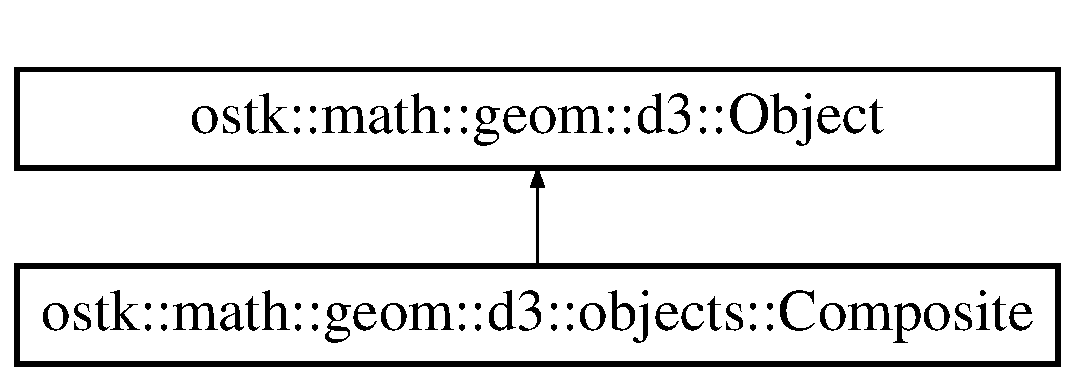
\includegraphics[height=2.000000cm]{classostk_1_1math_1_1geom_1_1d3_1_1objects_1_1_composite}
\end{center}
\end{figure}
\doxysubsection*{Public Types}
\begin{DoxyCompactItemize}
\item 
typedef Array$<$ Unique$<$ \mbox{\hyperlink{classostk_1_1math_1_1geom_1_1d3_1_1_object}{Object}} $>$ $>$\+::\mbox{\hyperlink{classostk_1_1math_1_1geom_1_1d3_1_1objects_1_1_composite_ab1f78408fec2e435dc1172cf2675b0a9}{Const\+Iterator}} \mbox{\hyperlink{classostk_1_1math_1_1geom_1_1d3_1_1objects_1_1_composite_ab1f78408fec2e435dc1172cf2675b0a9}{Const\+Iterator}}
\end{DoxyCompactItemize}
\doxysubsection*{Public Member Functions}
\begin{DoxyCompactItemize}
\item 
\mbox{\hyperlink{classostk_1_1math_1_1geom_1_1d3_1_1objects_1_1_composite_aaecda2f184484d63a52de87706a37d4c}{Composite}} (const \mbox{\hyperlink{classostk_1_1math_1_1geom_1_1d3_1_1_object}{Object}} \&an\+Object)
\begin{DoxyCompactList}\small\item\em Constructor. \end{DoxyCompactList}\item 
\mbox{\hyperlink{classostk_1_1math_1_1geom_1_1d3_1_1objects_1_1_composite_a28d3ff898cd4385abf0fd73ddcb54ef2}{Composite}} (const Unique$<$ \mbox{\hyperlink{classostk_1_1math_1_1geom_1_1d3_1_1_object}{Object}} $>$ \&an\+Object\+U\+Ptr)
\begin{DoxyCompactList}\small\item\em Constructor. \end{DoxyCompactList}\item 
\mbox{\hyperlink{classostk_1_1math_1_1geom_1_1d3_1_1objects_1_1_composite_a936bd3f9d4a6ba02b91ba47c61361b21}{Composite}} (Array$<$ Unique$<$ \mbox{\hyperlink{classostk_1_1math_1_1geom_1_1d3_1_1_object}{Object}} $>$$>$ \&\&an\+Object\+Array)
\begin{DoxyCompactList}\small\item\em Constructor. \end{DoxyCompactList}\item 
\mbox{\hyperlink{classostk_1_1math_1_1geom_1_1d3_1_1objects_1_1_composite_a8682632cf01c97cf9b6e621c8e6ce5db}{Composite}} (const \mbox{\hyperlink{classostk_1_1math_1_1geom_1_1d3_1_1objects_1_1_composite}{Composite}} \&a\+Composite)
\begin{DoxyCompactList}\small\item\em Copy constructor. \end{DoxyCompactList}\item 
virtual \mbox{\hyperlink{classostk_1_1math_1_1geom_1_1d3_1_1objects_1_1_composite}{Composite}} $\ast$ \mbox{\hyperlink{classostk_1_1math_1_1geom_1_1d3_1_1objects_1_1_composite_a3fa42c990116bf5537c943c404fa8fdd}{clone}} () const override
\begin{DoxyCompactList}\small\item\em Clone composite. \end{DoxyCompactList}\item 
\mbox{\hyperlink{classostk_1_1math_1_1geom_1_1d3_1_1objects_1_1_composite}{Composite}} \& \mbox{\hyperlink{classostk_1_1math_1_1geom_1_1d3_1_1objects_1_1_composite_a0e0a4a03302ae92926d8f4a94a3b1291}{operator=}} (const \mbox{\hyperlink{classostk_1_1math_1_1geom_1_1d3_1_1objects_1_1_composite}{Composite}} \&a\+Composite)
\begin{DoxyCompactList}\small\item\em Copy assignment operator. \end{DoxyCompactList}\item 
bool \mbox{\hyperlink{classostk_1_1math_1_1geom_1_1d3_1_1objects_1_1_composite_aa41f70a711077a4b59937fddef380150}{operator==}} (const \mbox{\hyperlink{classostk_1_1math_1_1geom_1_1d3_1_1objects_1_1_composite}{Composite}} \&a\+Composite) const
\begin{DoxyCompactList}\small\item\em Equal to operator. \end{DoxyCompactList}\item 
bool \mbox{\hyperlink{classostk_1_1math_1_1geom_1_1d3_1_1objects_1_1_composite_aa215a94dadd9a8912760c5c5ec4eb6e1}{operator!=}} (const \mbox{\hyperlink{classostk_1_1math_1_1geom_1_1d3_1_1objects_1_1_composite}{Composite}} \&a\+Composite) const
\begin{DoxyCompactList}\small\item\em Not equal to operator. \end{DoxyCompactList}\item 
\mbox{\hyperlink{classostk_1_1math_1_1geom_1_1d3_1_1objects_1_1_composite}{Composite}} \mbox{\hyperlink{classostk_1_1math_1_1geom_1_1d3_1_1objects_1_1_composite_a15a01835377b51a08b748762bc29411b}{operator+}} (const \mbox{\hyperlink{classostk_1_1math_1_1geom_1_1d3_1_1objects_1_1_composite}{Composite}} \&a\+Composite) const
\begin{DoxyCompactList}\small\item\em Addition operator (composite concatenation) \end{DoxyCompactList}\item 
\mbox{\hyperlink{classostk_1_1math_1_1geom_1_1d3_1_1objects_1_1_composite}{Composite}} \& \mbox{\hyperlink{classostk_1_1math_1_1geom_1_1d3_1_1objects_1_1_composite_aca2c415b82aee0b6acfae16675f1391e}{operator+=}} (const \mbox{\hyperlink{classostk_1_1math_1_1geom_1_1d3_1_1objects_1_1_composite}{Composite}} \&a\+Composite)
\begin{DoxyCompactList}\small\item\em Addition assignment operator (composite concatenation) \end{DoxyCompactList}\item 
virtual bool \mbox{\hyperlink{classostk_1_1math_1_1geom_1_1d3_1_1objects_1_1_composite_afda60d7f0111f98729e9c9d96ba4e1d5}{is\+Defined}} () const override
\begin{DoxyCompactList}\small\item\em Check if composite is defined. \end{DoxyCompactList}\item 
bool \mbox{\hyperlink{classostk_1_1math_1_1geom_1_1d3_1_1objects_1_1_composite_ac7b84d04a89c0cd2ef9c3538792ac168}{is\+Empty}} () const
\begin{DoxyCompactList}\small\item\em Check if composite is empty. \end{DoxyCompactList}\item 
{\footnotesize template$<$class Type $>$ }\\bool \mbox{\hyperlink{classostk_1_1math_1_1geom_1_1d3_1_1objects_1_1_composite_acbe01e7ef63382a16aa0b33f10d7a620}{is}} () const
\begin{DoxyCompactList}\small\item\em Returns true if composite can be converted to underlying object. \end{DoxyCompactList}\item 
{\footnotesize template$<$class Type $>$ }\\const Type \& \mbox{\hyperlink{classostk_1_1math_1_1geom_1_1d3_1_1objects_1_1_composite_a183fda79f9c329411533a390c77885ef}{as}} () const
\begin{DoxyCompactList}\small\item\em Access composite as its underlying object. \end{DoxyCompactList}\item 
bool \mbox{\hyperlink{classostk_1_1math_1_1geom_1_1d3_1_1objects_1_1_composite_a1064214841e9cc22475e0683fb16bce7}{intersects}} (const \mbox{\hyperlink{classostk_1_1math_1_1geom_1_1d3_1_1_object}{Object}} \&an\+Object) const
\begin{DoxyCompactList}\small\item\em Check if composite intersects object. \end{DoxyCompactList}\item 
bool \mbox{\hyperlink{classostk_1_1math_1_1geom_1_1d3_1_1objects_1_1_composite_a60a7aeb9a36d573e717ad6e191219201}{intersects}} (const \mbox{\hyperlink{classostk_1_1math_1_1geom_1_1d3_1_1objects_1_1_composite}{Composite}} \&a\+Composite) const
\begin{DoxyCompactList}\small\item\em Check if composite intersects composite. \end{DoxyCompactList}\item 
bool \mbox{\hyperlink{classostk_1_1math_1_1geom_1_1d3_1_1objects_1_1_composite_abe810bb7e17c444b1b556053e32750d1}{contains}} (const \mbox{\hyperlink{classostk_1_1math_1_1geom_1_1d3_1_1_object}{Object}} \&an\+Object) const
\begin{DoxyCompactList}\small\item\em Check if composite contains object. \end{DoxyCompactList}\item 
bool \mbox{\hyperlink{classostk_1_1math_1_1geom_1_1d3_1_1objects_1_1_composite_a54395e684abc0b64a629808e3c478e52}{contains}} (const \mbox{\hyperlink{classostk_1_1math_1_1geom_1_1d3_1_1objects_1_1_composite}{Composite}} \&a\+Composite) const
\begin{DoxyCompactList}\small\item\em Check if composite contains composite. \end{DoxyCompactList}\item 
const \mbox{\hyperlink{classostk_1_1math_1_1geom_1_1d3_1_1_object}{Object}} \& \mbox{\hyperlink{classostk_1_1math_1_1geom_1_1d3_1_1objects_1_1_composite_ad9eccbd18d6c474cb252221f0a9be915}{access\+Object\+At}} (const Index \&an\+Index) const
\begin{DoxyCompactList}\small\item\em Access object at index. \end{DoxyCompactList}\item 
const Array$<$ Unique$<$ \mbox{\hyperlink{classostk_1_1math_1_1geom_1_1d3_1_1_object}{Object}} $>$ $>$ \& \mbox{\hyperlink{classostk_1_1math_1_1geom_1_1d3_1_1objects_1_1_composite_a88392e0fefef248703057a22d17b90af}{access\+Objects}} () const
\begin{DoxyCompactList}\small\item\em Access objects in composite. \end{DoxyCompactList}\item 
Size \mbox{\hyperlink{classostk_1_1math_1_1geom_1_1d3_1_1objects_1_1_composite_a254785a50dc8deece73e24d2991704b6}{get\+Object\+Count}} () const
\begin{DoxyCompactList}\small\item\em Get number of objects in composite. \end{DoxyCompactList}\item 
\mbox{\hyperlink{classostk_1_1math_1_1geom_1_1d3_1_1_intersection}{Intersection}} \mbox{\hyperlink{classostk_1_1math_1_1geom_1_1d3_1_1objects_1_1_composite_a5c234652e274b4c2df015f89c2d3e90f}{intersection\+With}} (const \mbox{\hyperlink{classostk_1_1math_1_1geom_1_1d3_1_1_object}{Object}} \&an\+Object) const
\begin{DoxyCompactList}\small\item\em Compute intersection of composite with object. \end{DoxyCompactList}\item 
\mbox{\hyperlink{classostk_1_1math_1_1geom_1_1d3_1_1_intersection}{Intersection}} \mbox{\hyperlink{classostk_1_1math_1_1geom_1_1d3_1_1objects_1_1_composite_a4f5650ad091ee2009dd7b4cd135993bf}{intersection\+With}} (const \mbox{\hyperlink{classostk_1_1math_1_1geom_1_1d3_1_1objects_1_1_composite}{Composite}} \&a\+Composite) const
\begin{DoxyCompactList}\small\item\em Compute intersection of composite with composite. \end{DoxyCompactList}\item 
\mbox{\hyperlink{classostk_1_1math_1_1geom_1_1d3_1_1objects_1_1_composite_ab1f78408fec2e435dc1172cf2675b0a9}{Composite\+::\+Const\+Iterator}} \mbox{\hyperlink{classostk_1_1math_1_1geom_1_1d3_1_1objects_1_1_composite_ab94b6cd4186515bdc1fa246756fec3cb}{begin}} () const
\begin{DoxyCompactList}\small\item\em Get const iterator to begin. \end{DoxyCompactList}\item 
\mbox{\hyperlink{classostk_1_1math_1_1geom_1_1d3_1_1objects_1_1_composite_ab1f78408fec2e435dc1172cf2675b0a9}{Composite\+::\+Const\+Iterator}} \mbox{\hyperlink{classostk_1_1math_1_1geom_1_1d3_1_1objects_1_1_composite_abaaf231b9d0b5924ceb2b89db38cfe25}{end}} () const
\begin{DoxyCompactList}\small\item\em Get const iterator to end. \end{DoxyCompactList}\item 
virtual void \mbox{\hyperlink{classostk_1_1math_1_1geom_1_1d3_1_1objects_1_1_composite_afa4ff037d2ab625c650ef0e45c6ea4e6}{print}} (std\+::ostream \&an\+Output\+Stream, bool display\+Decorators=true) const override
\begin{DoxyCompactList}\small\item\em Print composite. \end{DoxyCompactList}\item 
virtual void \mbox{\hyperlink{classostk_1_1math_1_1geom_1_1d3_1_1objects_1_1_composite_a2d99d6b4096c2f5ba3175f886e2e2c7d}{apply\+Transformation}} (const \mbox{\hyperlink{classostk_1_1math_1_1geom_1_1d3_1_1_transformation}{Transformation}} \&a\+Transformation) override
\begin{DoxyCompactList}\small\item\em Apply transformation to composite. \end{DoxyCompactList}\end{DoxyCompactItemize}
\doxysubsection*{Static Public Member Functions}
\begin{DoxyCompactItemize}
\item 
static \mbox{\hyperlink{classostk_1_1math_1_1geom_1_1d3_1_1objects_1_1_composite}{Composite}} \mbox{\hyperlink{classostk_1_1math_1_1geom_1_1d3_1_1objects_1_1_composite_abd7585518f349e7d599a81102f9e0e41}{Undefined}} ()
\begin{DoxyCompactList}\small\item\em Constructs an undefined composite. \end{DoxyCompactList}\item 
static \mbox{\hyperlink{classostk_1_1math_1_1geom_1_1d3_1_1objects_1_1_composite}{Composite}} \mbox{\hyperlink{classostk_1_1math_1_1geom_1_1d3_1_1objects_1_1_composite_ab6ca471e3e731465d64148506869c93d}{Empty}} ()
\begin{DoxyCompactList}\small\item\em Constructs an empty composite. \end{DoxyCompactList}\end{DoxyCompactItemize}


\doxysubsection{Detailed Description}
\mbox{\hyperlink{classostk_1_1math_1_1geom_1_1d3_1_1objects_1_1_composite}{Composite}} object. 

\doxysubsection{Member Typedef Documentation}
\mbox{\Hypertarget{classostk_1_1math_1_1geom_1_1d3_1_1objects_1_1_composite_ab1f78408fec2e435dc1172cf2675b0a9}\label{classostk_1_1math_1_1geom_1_1d3_1_1objects_1_1_composite_ab1f78408fec2e435dc1172cf2675b0a9}} 
\index{ostk::math::geom::d3::objects::Composite@{ostk::math::geom::d3::objects::Composite}!ConstIterator@{ConstIterator}}
\index{ConstIterator@{ConstIterator}!ostk::math::geom::d3::objects::Composite@{ostk::math::geom::d3::objects::Composite}}
\doxysubsubsection{\texorpdfstring{ConstIterator}{ConstIterator}}
{\footnotesize\ttfamily typedef Array$<$Unique$<$\mbox{\hyperlink{classostk_1_1math_1_1geom_1_1d3_1_1_object}{Object}}$>$ $>$\+::\mbox{\hyperlink{classostk_1_1math_1_1geom_1_1d3_1_1objects_1_1_composite_ab1f78408fec2e435dc1172cf2675b0a9}{Const\+Iterator}} \mbox{\hyperlink{classostk_1_1math_1_1geom_1_1d3_1_1objects_1_1_composite_ab1f78408fec2e435dc1172cf2675b0a9}{ostk\+::math\+::geom\+::d3\+::objects\+::\+Composite\+::\+Const\+Iterator}}}



\doxysubsection{Constructor \& Destructor Documentation}
\mbox{\Hypertarget{classostk_1_1math_1_1geom_1_1d3_1_1objects_1_1_composite_aaecda2f184484d63a52de87706a37d4c}\label{classostk_1_1math_1_1geom_1_1d3_1_1objects_1_1_composite_aaecda2f184484d63a52de87706a37d4c}} 
\index{ostk::math::geom::d3::objects::Composite@{ostk::math::geom::d3::objects::Composite}!Composite@{Composite}}
\index{Composite@{Composite}!ostk::math::geom::d3::objects::Composite@{ostk::math::geom::d3::objects::Composite}}
\doxysubsubsection{\texorpdfstring{Composite()}{Composite()}\hspace{0.1cm}{\footnotesize\ttfamily [1/4]}}
{\footnotesize\ttfamily ostk\+::math\+::geom\+::d3\+::objects\+::\+Composite\+::\+Composite (\begin{DoxyParamCaption}\item[{const \mbox{\hyperlink{classostk_1_1math_1_1geom_1_1d3_1_1_object}{Object}} \&}]{an\+Object }\end{DoxyParamCaption})\hspace{0.3cm}{\ttfamily [explicit]}}



Constructor. 


\begin{DoxyParams}[1]{Parameters}
\mbox{\texttt{ in}}  & {\em an\+Object} & An object \\
\hline
\end{DoxyParams}
\mbox{\Hypertarget{classostk_1_1math_1_1geom_1_1d3_1_1objects_1_1_composite_a28d3ff898cd4385abf0fd73ddcb54ef2}\label{classostk_1_1math_1_1geom_1_1d3_1_1objects_1_1_composite_a28d3ff898cd4385abf0fd73ddcb54ef2}} 
\index{ostk::math::geom::d3::objects::Composite@{ostk::math::geom::d3::objects::Composite}!Composite@{Composite}}
\index{Composite@{Composite}!ostk::math::geom::d3::objects::Composite@{ostk::math::geom::d3::objects::Composite}}
\doxysubsubsection{\texorpdfstring{Composite()}{Composite()}\hspace{0.1cm}{\footnotesize\ttfamily [2/4]}}
{\footnotesize\ttfamily ostk\+::math\+::geom\+::d3\+::objects\+::\+Composite\+::\+Composite (\begin{DoxyParamCaption}\item[{const Unique$<$ \mbox{\hyperlink{classostk_1_1math_1_1geom_1_1d3_1_1_object}{Object}} $>$ \&}]{an\+Object\+U\+Ptr }\end{DoxyParamCaption})\hspace{0.3cm}{\ttfamily [explicit]}}



Constructor. 


\begin{DoxyParams}[1]{Parameters}
\mbox{\texttt{ in}}  & {\em an\+Object\+U\+Ptr} & A unique pointer to object \\
\hline
\end{DoxyParams}
\mbox{\Hypertarget{classostk_1_1math_1_1geom_1_1d3_1_1objects_1_1_composite_a936bd3f9d4a6ba02b91ba47c61361b21}\label{classostk_1_1math_1_1geom_1_1d3_1_1objects_1_1_composite_a936bd3f9d4a6ba02b91ba47c61361b21}} 
\index{ostk::math::geom::d3::objects::Composite@{ostk::math::geom::d3::objects::Composite}!Composite@{Composite}}
\index{Composite@{Composite}!ostk::math::geom::d3::objects::Composite@{ostk::math::geom::d3::objects::Composite}}
\doxysubsubsection{\texorpdfstring{Composite()}{Composite()}\hspace{0.1cm}{\footnotesize\ttfamily [3/4]}}
{\footnotesize\ttfamily ostk\+::math\+::geom\+::d3\+::objects\+::\+Composite\+::\+Composite (\begin{DoxyParamCaption}\item[{Array$<$ Unique$<$ \mbox{\hyperlink{classostk_1_1math_1_1geom_1_1d3_1_1_object}{Object}} $>$$>$ \&\&}]{an\+Object\+Array }\end{DoxyParamCaption})\hspace{0.3cm}{\ttfamily [explicit]}}



Constructor. 


\begin{DoxyParams}[1]{Parameters}
\mbox{\texttt{ in}}  & {\em an\+Object\+Array} & An array of unique pointers to object \\
\hline
\end{DoxyParams}
\mbox{\Hypertarget{classostk_1_1math_1_1geom_1_1d3_1_1objects_1_1_composite_a8682632cf01c97cf9b6e621c8e6ce5db}\label{classostk_1_1math_1_1geom_1_1d3_1_1objects_1_1_composite_a8682632cf01c97cf9b6e621c8e6ce5db}} 
\index{ostk::math::geom::d3::objects::Composite@{ostk::math::geom::d3::objects::Composite}!Composite@{Composite}}
\index{Composite@{Composite}!ostk::math::geom::d3::objects::Composite@{ostk::math::geom::d3::objects::Composite}}
\doxysubsubsection{\texorpdfstring{Composite()}{Composite()}\hspace{0.1cm}{\footnotesize\ttfamily [4/4]}}
{\footnotesize\ttfamily ostk\+::math\+::geom\+::d3\+::objects\+::\+Composite\+::\+Composite (\begin{DoxyParamCaption}\item[{const \mbox{\hyperlink{classostk_1_1math_1_1geom_1_1d3_1_1objects_1_1_composite}{Composite}} \&}]{a\+Composite }\end{DoxyParamCaption})}



Copy constructor. 


\begin{DoxyParams}[1]{Parameters}
\mbox{\texttt{ in}}  & {\em a\+Composite} & A composite \\
\hline
\end{DoxyParams}


\doxysubsection{Member Function Documentation}
\mbox{\Hypertarget{classostk_1_1math_1_1geom_1_1d3_1_1objects_1_1_composite_ad9eccbd18d6c474cb252221f0a9be915}\label{classostk_1_1math_1_1geom_1_1d3_1_1objects_1_1_composite_ad9eccbd18d6c474cb252221f0a9be915}} 
\index{ostk::math::geom::d3::objects::Composite@{ostk::math::geom::d3::objects::Composite}!accessObjectAt@{accessObjectAt}}
\index{accessObjectAt@{accessObjectAt}!ostk::math::geom::d3::objects::Composite@{ostk::math::geom::d3::objects::Composite}}
\doxysubsubsection{\texorpdfstring{accessObjectAt()}{accessObjectAt()}}
{\footnotesize\ttfamily const \mbox{\hyperlink{classostk_1_1math_1_1geom_1_1d3_1_1_object}{Object}} \& ostk\+::math\+::geom\+::d3\+::objects\+::\+Composite\+::access\+Object\+At (\begin{DoxyParamCaption}\item[{const Index \&}]{an\+Index }\end{DoxyParamCaption}) const}



Access object at index. 


\begin{DoxyParams}[1]{Parameters}
\mbox{\texttt{ in}}  & {\em an\+Index} & An object index \\
\hline
\end{DoxyParams}
\begin{DoxyReturn}{Returns}
Reference to object 
\end{DoxyReturn}
\mbox{\Hypertarget{classostk_1_1math_1_1geom_1_1d3_1_1objects_1_1_composite_a88392e0fefef248703057a22d17b90af}\label{classostk_1_1math_1_1geom_1_1d3_1_1objects_1_1_composite_a88392e0fefef248703057a22d17b90af}} 
\index{ostk::math::geom::d3::objects::Composite@{ostk::math::geom::d3::objects::Composite}!accessObjects@{accessObjects}}
\index{accessObjects@{accessObjects}!ostk::math::geom::d3::objects::Composite@{ostk::math::geom::d3::objects::Composite}}
\doxysubsubsection{\texorpdfstring{accessObjects()}{accessObjects()}}
{\footnotesize\ttfamily const Array$<$ Unique$<$ \mbox{\hyperlink{classostk_1_1math_1_1geom_1_1d3_1_1_object}{Object}} $>$ $>$ \& ostk\+::math\+::geom\+::d3\+::objects\+::\+Composite\+::access\+Objects (\begin{DoxyParamCaption}{ }\end{DoxyParamCaption}) const}



Access objects in composite. 

\begin{DoxyReturn}{Returns}
Reference to objects in composite 
\end{DoxyReturn}
\mbox{\Hypertarget{classostk_1_1math_1_1geom_1_1d3_1_1objects_1_1_composite_a2d99d6b4096c2f5ba3175f886e2e2c7d}\label{classostk_1_1math_1_1geom_1_1d3_1_1objects_1_1_composite_a2d99d6b4096c2f5ba3175f886e2e2c7d}} 
\index{ostk::math::geom::d3::objects::Composite@{ostk::math::geom::d3::objects::Composite}!applyTransformation@{applyTransformation}}
\index{applyTransformation@{applyTransformation}!ostk::math::geom::d3::objects::Composite@{ostk::math::geom::d3::objects::Composite}}
\doxysubsubsection{\texorpdfstring{applyTransformation()}{applyTransformation()}}
{\footnotesize\ttfamily void ostk\+::math\+::geom\+::d3\+::objects\+::\+Composite\+::apply\+Transformation (\begin{DoxyParamCaption}\item[{const \mbox{\hyperlink{classostk_1_1math_1_1geom_1_1d3_1_1_transformation}{Transformation}} \&}]{a\+Transformation }\end{DoxyParamCaption})\hspace{0.3cm}{\ttfamily [override]}, {\ttfamily [virtual]}}



Apply transformation to composite. 


\begin{DoxyParams}[1]{Parameters}
\mbox{\texttt{ in}}  & {\em a\+Transformation} & A transformation \\
\hline
\end{DoxyParams}


Implements \mbox{\hyperlink{classostk_1_1math_1_1geom_1_1d3_1_1_object_ae9194dd6d2bb4df09292ffc84dccdb1d}{ostk\+::math\+::geom\+::d3\+::\+Object}}.

\mbox{\Hypertarget{classostk_1_1math_1_1geom_1_1d3_1_1objects_1_1_composite_a183fda79f9c329411533a390c77885ef}\label{classostk_1_1math_1_1geom_1_1d3_1_1objects_1_1_composite_a183fda79f9c329411533a390c77885ef}} 
\index{ostk::math::geom::d3::objects::Composite@{ostk::math::geom::d3::objects::Composite}!as@{as}}
\index{as@{as}!ostk::math::geom::d3::objects::Composite@{ostk::math::geom::d3::objects::Composite}}
\doxysubsubsection{\texorpdfstring{as()}{as()}}
{\footnotesize\ttfamily template$<$class Type $>$ \\
const Type\& ostk\+::math\+::geom\+::d3\+::objects\+::\+Composite\+::as (\begin{DoxyParamCaption}{ }\end{DoxyParamCaption}) const\hspace{0.3cm}{\ttfamily [inline]}}



Access composite as its underlying object. 

\begin{DoxyVerb}                Only valid if the composite only contains one object.
\end{DoxyVerb}


\begin{DoxyReturn}{Returns}
Reference to underlying object 
\end{DoxyReturn}
\mbox{\Hypertarget{classostk_1_1math_1_1geom_1_1d3_1_1objects_1_1_composite_ab94b6cd4186515bdc1fa246756fec3cb}\label{classostk_1_1math_1_1geom_1_1d3_1_1objects_1_1_composite_ab94b6cd4186515bdc1fa246756fec3cb}} 
\index{ostk::math::geom::d3::objects::Composite@{ostk::math::geom::d3::objects::Composite}!begin@{begin}}
\index{begin@{begin}!ostk::math::geom::d3::objects::Composite@{ostk::math::geom::d3::objects::Composite}}
\doxysubsubsection{\texorpdfstring{begin()}{begin()}}
{\footnotesize\ttfamily \mbox{\hyperlink{classostk_1_1math_1_1geom_1_1d3_1_1objects_1_1_composite_ab1f78408fec2e435dc1172cf2675b0a9}{Composite\+::\+Const\+Iterator}} ostk\+::math\+::geom\+::d3\+::objects\+::\+Composite\+::begin (\begin{DoxyParamCaption}{ }\end{DoxyParamCaption}) const}



Get const iterator to begin. 

\begin{DoxyReturn}{Returns}
Const iterator to begin 
\end{DoxyReturn}
\mbox{\Hypertarget{classostk_1_1math_1_1geom_1_1d3_1_1objects_1_1_composite_a3fa42c990116bf5537c943c404fa8fdd}\label{classostk_1_1math_1_1geom_1_1d3_1_1objects_1_1_composite_a3fa42c990116bf5537c943c404fa8fdd}} 
\index{ostk::math::geom::d3::objects::Composite@{ostk::math::geom::d3::objects::Composite}!clone@{clone}}
\index{clone@{clone}!ostk::math::geom::d3::objects::Composite@{ostk::math::geom::d3::objects::Composite}}
\doxysubsubsection{\texorpdfstring{clone()}{clone()}}
{\footnotesize\ttfamily \mbox{\hyperlink{classostk_1_1math_1_1geom_1_1d3_1_1objects_1_1_composite}{Composite}} $\ast$ ostk\+::math\+::geom\+::d3\+::objects\+::\+Composite\+::clone (\begin{DoxyParamCaption}{ }\end{DoxyParamCaption}) const\hspace{0.3cm}{\ttfamily [override]}, {\ttfamily [virtual]}}



Clone composite. 

\begin{DoxyReturn}{Returns}
Pointer to cloned composite 
\end{DoxyReturn}


Implements \mbox{\hyperlink{classostk_1_1math_1_1geom_1_1d3_1_1_object_a676013f9555f6492687f9809b2db887b}{ostk\+::math\+::geom\+::d3\+::\+Object}}.

\mbox{\Hypertarget{classostk_1_1math_1_1geom_1_1d3_1_1objects_1_1_composite_a54395e684abc0b64a629808e3c478e52}\label{classostk_1_1math_1_1geom_1_1d3_1_1objects_1_1_composite_a54395e684abc0b64a629808e3c478e52}} 
\index{ostk::math::geom::d3::objects::Composite@{ostk::math::geom::d3::objects::Composite}!contains@{contains}}
\index{contains@{contains}!ostk::math::geom::d3::objects::Composite@{ostk::math::geom::d3::objects::Composite}}
\doxysubsubsection{\texorpdfstring{contains()}{contains()}\hspace{0.1cm}{\footnotesize\ttfamily [1/2]}}
{\footnotesize\ttfamily bool ostk\+::math\+::geom\+::d3\+::objects\+::\+Composite\+::contains (\begin{DoxyParamCaption}\item[{const \mbox{\hyperlink{classostk_1_1math_1_1geom_1_1d3_1_1objects_1_1_composite}{Composite}} \&}]{a\+Composite }\end{DoxyParamCaption}) const}



Check if composite contains composite. 


\begin{DoxyParams}[1]{Parameters}
\mbox{\texttt{ in}}  & {\em a\+Composite} & A composite \\
\hline
\end{DoxyParams}
\begin{DoxyReturn}{Returns}
True if composite contains composite 
\end{DoxyReturn}
\mbox{\Hypertarget{classostk_1_1math_1_1geom_1_1d3_1_1objects_1_1_composite_abe810bb7e17c444b1b556053e32750d1}\label{classostk_1_1math_1_1geom_1_1d3_1_1objects_1_1_composite_abe810bb7e17c444b1b556053e32750d1}} 
\index{ostk::math::geom::d3::objects::Composite@{ostk::math::geom::d3::objects::Composite}!contains@{contains}}
\index{contains@{contains}!ostk::math::geom::d3::objects::Composite@{ostk::math::geom::d3::objects::Composite}}
\doxysubsubsection{\texorpdfstring{contains()}{contains()}\hspace{0.1cm}{\footnotesize\ttfamily [2/2]}}
{\footnotesize\ttfamily bool ostk\+::math\+::geom\+::d3\+::objects\+::\+Composite\+::contains (\begin{DoxyParamCaption}\item[{const \mbox{\hyperlink{classostk_1_1math_1_1geom_1_1d3_1_1_object}{Object}} \&}]{an\+Object }\end{DoxyParamCaption}) const\hspace{0.3cm}{\ttfamily [virtual]}}



Check if composite contains object. 


\begin{DoxyParams}[1]{Parameters}
\mbox{\texttt{ in}}  & {\em an\+Object} & An object \\
\hline
\end{DoxyParams}
\begin{DoxyReturn}{Returns}
True if composite contains object 
\end{DoxyReturn}


Reimplemented from \mbox{\hyperlink{classostk_1_1math_1_1geom_1_1d3_1_1_object_a97edbd679b50c4663d3ab20c65cea4b9}{ostk\+::math\+::geom\+::d3\+::\+Object}}.

\mbox{\Hypertarget{classostk_1_1math_1_1geom_1_1d3_1_1objects_1_1_composite_ab6ca471e3e731465d64148506869c93d}\label{classostk_1_1math_1_1geom_1_1d3_1_1objects_1_1_composite_ab6ca471e3e731465d64148506869c93d}} 
\index{ostk::math::geom::d3::objects::Composite@{ostk::math::geom::d3::objects::Composite}!Empty@{Empty}}
\index{Empty@{Empty}!ostk::math::geom::d3::objects::Composite@{ostk::math::geom::d3::objects::Composite}}
\doxysubsubsection{\texorpdfstring{Empty()}{Empty()}}
{\footnotesize\ttfamily \mbox{\hyperlink{classostk_1_1math_1_1geom_1_1d3_1_1objects_1_1_composite}{Composite}} ostk\+::math\+::geom\+::d3\+::objects\+::\+Composite\+::\+Empty (\begin{DoxyParamCaption}{ }\end{DoxyParamCaption})\hspace{0.3cm}{\ttfamily [static]}}



Constructs an empty composite. 


\begin{DoxyCode}{0}
\DoxyCodeLine{\mbox{\hyperlink{classostk_1_1math_1_1geom_1_1d3_1_1objects_1_1_composite_aaecda2f184484d63a52de87706a37d4c}{Composite}} composite = \mbox{\hyperlink{classostk_1_1math_1_1geom_1_1d3_1_1objects_1_1_composite_ab6ca471e3e731465d64148506869c93d}{Composite::Empty}}() ;}
\end{DoxyCode}


\begin{DoxyReturn}{Returns}
Empty composite 
\end{DoxyReturn}
\mbox{\Hypertarget{classostk_1_1math_1_1geom_1_1d3_1_1objects_1_1_composite_abaaf231b9d0b5924ceb2b89db38cfe25}\label{classostk_1_1math_1_1geom_1_1d3_1_1objects_1_1_composite_abaaf231b9d0b5924ceb2b89db38cfe25}} 
\index{ostk::math::geom::d3::objects::Composite@{ostk::math::geom::d3::objects::Composite}!end@{end}}
\index{end@{end}!ostk::math::geom::d3::objects::Composite@{ostk::math::geom::d3::objects::Composite}}
\doxysubsubsection{\texorpdfstring{end()}{end()}}
{\footnotesize\ttfamily \mbox{\hyperlink{classostk_1_1math_1_1geom_1_1d3_1_1objects_1_1_composite_ab1f78408fec2e435dc1172cf2675b0a9}{Composite\+::\+Const\+Iterator}} ostk\+::math\+::geom\+::d3\+::objects\+::\+Composite\+::end (\begin{DoxyParamCaption}{ }\end{DoxyParamCaption}) const}



Get const iterator to end. 

\begin{DoxyReturn}{Returns}
Const iterator to end 
\end{DoxyReturn}
\mbox{\Hypertarget{classostk_1_1math_1_1geom_1_1d3_1_1objects_1_1_composite_a254785a50dc8deece73e24d2991704b6}\label{classostk_1_1math_1_1geom_1_1d3_1_1objects_1_1_composite_a254785a50dc8deece73e24d2991704b6}} 
\index{ostk::math::geom::d3::objects::Composite@{ostk::math::geom::d3::objects::Composite}!getObjectCount@{getObjectCount}}
\index{getObjectCount@{getObjectCount}!ostk::math::geom::d3::objects::Composite@{ostk::math::geom::d3::objects::Composite}}
\doxysubsubsection{\texorpdfstring{getObjectCount()}{getObjectCount()}}
{\footnotesize\ttfamily Size ostk\+::math\+::geom\+::d3\+::objects\+::\+Composite\+::get\+Object\+Count (\begin{DoxyParamCaption}{ }\end{DoxyParamCaption}) const}



Get number of objects in composite. 

\begin{DoxyReturn}{Returns}
Number of objects in composite 
\end{DoxyReturn}
\mbox{\Hypertarget{classostk_1_1math_1_1geom_1_1d3_1_1objects_1_1_composite_a4f5650ad091ee2009dd7b4cd135993bf}\label{classostk_1_1math_1_1geom_1_1d3_1_1objects_1_1_composite_a4f5650ad091ee2009dd7b4cd135993bf}} 
\index{ostk::math::geom::d3::objects::Composite@{ostk::math::geom::d3::objects::Composite}!intersectionWith@{intersectionWith}}
\index{intersectionWith@{intersectionWith}!ostk::math::geom::d3::objects::Composite@{ostk::math::geom::d3::objects::Composite}}
\doxysubsubsection{\texorpdfstring{intersectionWith()}{intersectionWith()}\hspace{0.1cm}{\footnotesize\ttfamily [1/2]}}
{\footnotesize\ttfamily \mbox{\hyperlink{classostk_1_1math_1_1geom_1_1d3_1_1_intersection}{Intersection}} ostk\+::math\+::geom\+::d3\+::objects\+::\+Composite\+::intersection\+With (\begin{DoxyParamCaption}\item[{const \mbox{\hyperlink{classostk_1_1math_1_1geom_1_1d3_1_1objects_1_1_composite}{Composite}} \&}]{a\+Composite }\end{DoxyParamCaption}) const}



Compute intersection of composite with composite. 


\begin{DoxyParams}[1]{Parameters}
\mbox{\texttt{ in}}  & {\em a\+Composite} & A composite \\
\hline
\end{DoxyParams}
\begin{DoxyReturn}{Returns}
\mbox{\hyperlink{classostk_1_1math_1_1geom_1_1d3_1_1_intersection}{Intersection}} of composite with composite 
\end{DoxyReturn}
\mbox{\Hypertarget{classostk_1_1math_1_1geom_1_1d3_1_1objects_1_1_composite_a5c234652e274b4c2df015f89c2d3e90f}\label{classostk_1_1math_1_1geom_1_1d3_1_1objects_1_1_composite_a5c234652e274b4c2df015f89c2d3e90f}} 
\index{ostk::math::geom::d3::objects::Composite@{ostk::math::geom::d3::objects::Composite}!intersectionWith@{intersectionWith}}
\index{intersectionWith@{intersectionWith}!ostk::math::geom::d3::objects::Composite@{ostk::math::geom::d3::objects::Composite}}
\doxysubsubsection{\texorpdfstring{intersectionWith()}{intersectionWith()}\hspace{0.1cm}{\footnotesize\ttfamily [2/2]}}
{\footnotesize\ttfamily \mbox{\hyperlink{classostk_1_1math_1_1geom_1_1d3_1_1_intersection}{Intersection}} ostk\+::math\+::geom\+::d3\+::objects\+::\+Composite\+::intersection\+With (\begin{DoxyParamCaption}\item[{const \mbox{\hyperlink{classostk_1_1math_1_1geom_1_1d3_1_1_object}{Object}} \&}]{an\+Object }\end{DoxyParamCaption}) const\hspace{0.3cm}{\ttfamily [virtual]}}



Compute intersection of composite with object. 


\begin{DoxyParams}[1]{Parameters}
\mbox{\texttt{ in}}  & {\em an\+Object} & An object \\
\hline
\end{DoxyParams}
\begin{DoxyReturn}{Returns}
\mbox{\hyperlink{classostk_1_1math_1_1geom_1_1d3_1_1_intersection}{Intersection}} of composite with object 
\end{DoxyReturn}


Reimplemented from \mbox{\hyperlink{classostk_1_1math_1_1geom_1_1d3_1_1_object_a04622921234740473c7731fa6c5bad0a}{ostk\+::math\+::geom\+::d3\+::\+Object}}.

\mbox{\Hypertarget{classostk_1_1math_1_1geom_1_1d3_1_1objects_1_1_composite_a60a7aeb9a36d573e717ad6e191219201}\label{classostk_1_1math_1_1geom_1_1d3_1_1objects_1_1_composite_a60a7aeb9a36d573e717ad6e191219201}} 
\index{ostk::math::geom::d3::objects::Composite@{ostk::math::geom::d3::objects::Composite}!intersects@{intersects}}
\index{intersects@{intersects}!ostk::math::geom::d3::objects::Composite@{ostk::math::geom::d3::objects::Composite}}
\doxysubsubsection{\texorpdfstring{intersects()}{intersects()}\hspace{0.1cm}{\footnotesize\ttfamily [1/2]}}
{\footnotesize\ttfamily bool ostk\+::math\+::geom\+::d3\+::objects\+::\+Composite\+::intersects (\begin{DoxyParamCaption}\item[{const \mbox{\hyperlink{classostk_1_1math_1_1geom_1_1d3_1_1objects_1_1_composite}{Composite}} \&}]{a\+Composite }\end{DoxyParamCaption}) const}



Check if composite intersects composite. 


\begin{DoxyParams}[1]{Parameters}
\mbox{\texttt{ in}}  & {\em a\+Composite} & A composite \\
\hline
\end{DoxyParams}
\begin{DoxyReturn}{Returns}
True if composite intersects composite 
\end{DoxyReturn}
\mbox{\Hypertarget{classostk_1_1math_1_1geom_1_1d3_1_1objects_1_1_composite_a1064214841e9cc22475e0683fb16bce7}\label{classostk_1_1math_1_1geom_1_1d3_1_1objects_1_1_composite_a1064214841e9cc22475e0683fb16bce7}} 
\index{ostk::math::geom::d3::objects::Composite@{ostk::math::geom::d3::objects::Composite}!intersects@{intersects}}
\index{intersects@{intersects}!ostk::math::geom::d3::objects::Composite@{ostk::math::geom::d3::objects::Composite}}
\doxysubsubsection{\texorpdfstring{intersects()}{intersects()}\hspace{0.1cm}{\footnotesize\ttfamily [2/2]}}
{\footnotesize\ttfamily bool ostk\+::math\+::geom\+::d3\+::objects\+::\+Composite\+::intersects (\begin{DoxyParamCaption}\item[{const \mbox{\hyperlink{classostk_1_1math_1_1geom_1_1d3_1_1_object}{Object}} \&}]{an\+Object }\end{DoxyParamCaption}) const\hspace{0.3cm}{\ttfamily [virtual]}}



Check if composite intersects object. 


\begin{DoxyParams}[1]{Parameters}
\mbox{\texttt{ in}}  & {\em an\+Object} & An object \\
\hline
\end{DoxyParams}
\begin{DoxyReturn}{Returns}
True if composite intersects object 
\end{DoxyReturn}


Reimplemented from \mbox{\hyperlink{classostk_1_1math_1_1geom_1_1d3_1_1_object_a99bfe722e7508a09a629c9eb972201e6}{ostk\+::math\+::geom\+::d3\+::\+Object}}.

\mbox{\Hypertarget{classostk_1_1math_1_1geom_1_1d3_1_1objects_1_1_composite_acbe01e7ef63382a16aa0b33f10d7a620}\label{classostk_1_1math_1_1geom_1_1d3_1_1objects_1_1_composite_acbe01e7ef63382a16aa0b33f10d7a620}} 
\index{ostk::math::geom::d3::objects::Composite@{ostk::math::geom::d3::objects::Composite}!is@{is}}
\index{is@{is}!ostk::math::geom::d3::objects::Composite@{ostk::math::geom::d3::objects::Composite}}
\doxysubsubsection{\texorpdfstring{is()}{is()}}
{\footnotesize\ttfamily template$<$class Type $>$ \\
bool ostk\+::math\+::geom\+::d3\+::objects\+::\+Composite\+::is (\begin{DoxyParamCaption}{ }\end{DoxyParamCaption}) const\hspace{0.3cm}{\ttfamily [inline]}}



Returns true if composite can be converted to underlying object. 

\begin{DoxyVerb}                Only valid if the composite only contains one object.
\end{DoxyVerb}


\begin{DoxyReturn}{Returns}
True if composite can be converted to underlying object 
\end{DoxyReturn}
\mbox{\Hypertarget{classostk_1_1math_1_1geom_1_1d3_1_1objects_1_1_composite_afda60d7f0111f98729e9c9d96ba4e1d5}\label{classostk_1_1math_1_1geom_1_1d3_1_1objects_1_1_composite_afda60d7f0111f98729e9c9d96ba4e1d5}} 
\index{ostk::math::geom::d3::objects::Composite@{ostk::math::geom::d3::objects::Composite}!isDefined@{isDefined}}
\index{isDefined@{isDefined}!ostk::math::geom::d3::objects::Composite@{ostk::math::geom::d3::objects::Composite}}
\doxysubsubsection{\texorpdfstring{isDefined()}{isDefined()}}
{\footnotesize\ttfamily bool ostk\+::math\+::geom\+::d3\+::objects\+::\+Composite\+::is\+Defined (\begin{DoxyParamCaption}{ }\end{DoxyParamCaption}) const\hspace{0.3cm}{\ttfamily [override]}, {\ttfamily [virtual]}}



Check if composite is defined. 


\begin{DoxyCode}{0}
\DoxyCodeLine{\mbox{\hyperlink{classostk_1_1math_1_1geom_1_1d3_1_1objects_1_1_composite_aaecda2f184484d63a52de87706a37d4c}{Composite}}(...).isDefined() ;}
\end{DoxyCode}


\begin{DoxyReturn}{Returns}
True if composite is defined 
\end{DoxyReturn}


Implements \mbox{\hyperlink{classostk_1_1math_1_1geom_1_1d3_1_1_object_a271a1964cd208be85ce9a0a429395ad8}{ostk\+::math\+::geom\+::d3\+::\+Object}}.

\mbox{\Hypertarget{classostk_1_1math_1_1geom_1_1d3_1_1objects_1_1_composite_ac7b84d04a89c0cd2ef9c3538792ac168}\label{classostk_1_1math_1_1geom_1_1d3_1_1objects_1_1_composite_ac7b84d04a89c0cd2ef9c3538792ac168}} 
\index{ostk::math::geom::d3::objects::Composite@{ostk::math::geom::d3::objects::Composite}!isEmpty@{isEmpty}}
\index{isEmpty@{isEmpty}!ostk::math::geom::d3::objects::Composite@{ostk::math::geom::d3::objects::Composite}}
\doxysubsubsection{\texorpdfstring{isEmpty()}{isEmpty()}}
{\footnotesize\ttfamily bool ostk\+::math\+::geom\+::d3\+::objects\+::\+Composite\+::is\+Empty (\begin{DoxyParamCaption}{ }\end{DoxyParamCaption}) const}



Check if composite is empty. 


\begin{DoxyCode}{0}
\DoxyCodeLine{\mbox{\hyperlink{classostk_1_1math_1_1geom_1_1d3_1_1objects_1_1_composite_aaecda2f184484d63a52de87706a37d4c}{Composite}}(...).isEmpty() ;}
\end{DoxyCode}


\begin{DoxyReturn}{Returns}
True if composite is empty 
\end{DoxyReturn}
\mbox{\Hypertarget{classostk_1_1math_1_1geom_1_1d3_1_1objects_1_1_composite_aa215a94dadd9a8912760c5c5ec4eb6e1}\label{classostk_1_1math_1_1geom_1_1d3_1_1objects_1_1_composite_aa215a94dadd9a8912760c5c5ec4eb6e1}} 
\index{ostk::math::geom::d3::objects::Composite@{ostk::math::geom::d3::objects::Composite}!operator"!=@{operator"!=}}
\index{operator"!=@{operator"!=}!ostk::math::geom::d3::objects::Composite@{ostk::math::geom::d3::objects::Composite}}
\doxysubsubsection{\texorpdfstring{operator"!=()}{operator!=()}}
{\footnotesize\ttfamily bool ostk\+::math\+::geom\+::d3\+::objects\+::\+Composite\+::operator!= (\begin{DoxyParamCaption}\item[{const \mbox{\hyperlink{classostk_1_1math_1_1geom_1_1d3_1_1objects_1_1_composite}{Composite}} \&}]{a\+Composite }\end{DoxyParamCaption}) const}



Not equal to operator. 


\begin{DoxyParams}[1]{Parameters}
\mbox{\texttt{ in}}  & {\em a\+Composite} & A composite object \\
\hline
\end{DoxyParams}
\begin{DoxyReturn}{Returns}
True if composites are not equal 
\end{DoxyReturn}
\mbox{\Hypertarget{classostk_1_1math_1_1geom_1_1d3_1_1objects_1_1_composite_a15a01835377b51a08b748762bc29411b}\label{classostk_1_1math_1_1geom_1_1d3_1_1objects_1_1_composite_a15a01835377b51a08b748762bc29411b}} 
\index{ostk::math::geom::d3::objects::Composite@{ostk::math::geom::d3::objects::Composite}!operator+@{operator+}}
\index{operator+@{operator+}!ostk::math::geom::d3::objects::Composite@{ostk::math::geom::d3::objects::Composite}}
\doxysubsubsection{\texorpdfstring{operator+()}{operator+()}}
{\footnotesize\ttfamily \mbox{\hyperlink{classostk_1_1math_1_1geom_1_1d3_1_1objects_1_1_composite}{Composite}} ostk\+::math\+::geom\+::d3\+::objects\+::\+Composite\+::operator+ (\begin{DoxyParamCaption}\item[{const \mbox{\hyperlink{classostk_1_1math_1_1geom_1_1d3_1_1objects_1_1_composite}{Composite}} \&}]{a\+Composite }\end{DoxyParamCaption}) const}



Addition operator (composite concatenation) 

\begin{DoxyVerb}                Concatenate (merge) composite with another composite.
\end{DoxyVerb}



\begin{DoxyParams}[1]{Parameters}
\mbox{\texttt{ in}}  & {\em a\+Composite} & A composite \\
\hline
\end{DoxyParams}
\begin{DoxyReturn}{Returns}
Concatenated composite 
\end{DoxyReturn}
\mbox{\Hypertarget{classostk_1_1math_1_1geom_1_1d3_1_1objects_1_1_composite_aca2c415b82aee0b6acfae16675f1391e}\label{classostk_1_1math_1_1geom_1_1d3_1_1objects_1_1_composite_aca2c415b82aee0b6acfae16675f1391e}} 
\index{ostk::math::geom::d3::objects::Composite@{ostk::math::geom::d3::objects::Composite}!operator+=@{operator+=}}
\index{operator+=@{operator+=}!ostk::math::geom::d3::objects::Composite@{ostk::math::geom::d3::objects::Composite}}
\doxysubsubsection{\texorpdfstring{operator+=()}{operator+=()}}
{\footnotesize\ttfamily \mbox{\hyperlink{classostk_1_1math_1_1geom_1_1d3_1_1objects_1_1_composite}{Composite}} \& ostk\+::math\+::geom\+::d3\+::objects\+::\+Composite\+::operator+= (\begin{DoxyParamCaption}\item[{const \mbox{\hyperlink{classostk_1_1math_1_1geom_1_1d3_1_1objects_1_1_composite}{Composite}} \&}]{a\+Composite }\end{DoxyParamCaption})}



Addition assignment operator (composite concatenation) 

\begin{DoxyVerb}                Concatenate (merge) composite with another composite.
\end{DoxyVerb}



\begin{DoxyParams}[1]{Parameters}
\mbox{\texttt{ in}}  & {\em a\+Composite} & A composite \\
\hline
\end{DoxyParams}
\begin{DoxyReturn}{Returns}
Reference to concatenated composite 
\end{DoxyReturn}
\mbox{\Hypertarget{classostk_1_1math_1_1geom_1_1d3_1_1objects_1_1_composite_a0e0a4a03302ae92926d8f4a94a3b1291}\label{classostk_1_1math_1_1geom_1_1d3_1_1objects_1_1_composite_a0e0a4a03302ae92926d8f4a94a3b1291}} 
\index{ostk::math::geom::d3::objects::Composite@{ostk::math::geom::d3::objects::Composite}!operator=@{operator=}}
\index{operator=@{operator=}!ostk::math::geom::d3::objects::Composite@{ostk::math::geom::d3::objects::Composite}}
\doxysubsubsection{\texorpdfstring{operator=()}{operator=()}}
{\footnotesize\ttfamily \mbox{\hyperlink{classostk_1_1math_1_1geom_1_1d3_1_1objects_1_1_composite}{Composite}} \& ostk\+::math\+::geom\+::d3\+::objects\+::\+Composite\+::operator= (\begin{DoxyParamCaption}\item[{const \mbox{\hyperlink{classostk_1_1math_1_1geom_1_1d3_1_1objects_1_1_composite}{Composite}} \&}]{a\+Composite }\end{DoxyParamCaption})}



Copy assignment operator. 


\begin{DoxyParams}[1]{Parameters}
\mbox{\texttt{ in}}  & {\em a\+Composite} & A composite \\
\hline
\end{DoxyParams}
\begin{DoxyReturn}{Returns}
Reference to composite 
\end{DoxyReturn}
\mbox{\Hypertarget{classostk_1_1math_1_1geom_1_1d3_1_1objects_1_1_composite_aa41f70a711077a4b59937fddef380150}\label{classostk_1_1math_1_1geom_1_1d3_1_1objects_1_1_composite_aa41f70a711077a4b59937fddef380150}} 
\index{ostk::math::geom::d3::objects::Composite@{ostk::math::geom::d3::objects::Composite}!operator==@{operator==}}
\index{operator==@{operator==}!ostk::math::geom::d3::objects::Composite@{ostk::math::geom::d3::objects::Composite}}
\doxysubsubsection{\texorpdfstring{operator==()}{operator==()}}
{\footnotesize\ttfamily bool ostk\+::math\+::geom\+::d3\+::objects\+::\+Composite\+::operator== (\begin{DoxyParamCaption}\item[{const \mbox{\hyperlink{classostk_1_1math_1_1geom_1_1d3_1_1objects_1_1_composite}{Composite}} \&}]{a\+Composite }\end{DoxyParamCaption}) const}



Equal to operator. 


\begin{DoxyParams}[1]{Parameters}
\mbox{\texttt{ in}}  & {\em a\+Composite} & A composite object \\
\hline
\end{DoxyParams}
\begin{DoxyReturn}{Returns}
True if composites are equal 
\end{DoxyReturn}
\mbox{\Hypertarget{classostk_1_1math_1_1geom_1_1d3_1_1objects_1_1_composite_afa4ff037d2ab625c650ef0e45c6ea4e6}\label{classostk_1_1math_1_1geom_1_1d3_1_1objects_1_1_composite_afa4ff037d2ab625c650ef0e45c6ea4e6}} 
\index{ostk::math::geom::d3::objects::Composite@{ostk::math::geom::d3::objects::Composite}!print@{print}}
\index{print@{print}!ostk::math::geom::d3::objects::Composite@{ostk::math::geom::d3::objects::Composite}}
\doxysubsubsection{\texorpdfstring{print()}{print()}}
{\footnotesize\ttfamily void ostk\+::math\+::geom\+::d3\+::objects\+::\+Composite\+::print (\begin{DoxyParamCaption}\item[{std\+::ostream \&}]{an\+Output\+Stream,  }\item[{bool}]{display\+Decorators = {\ttfamily true} }\end{DoxyParamCaption}) const\hspace{0.3cm}{\ttfamily [override]}, {\ttfamily [virtual]}}



Print composite. 


\begin{DoxyParams}[1]{Parameters}
\mbox{\texttt{ in}}  & {\em an\+Output\+Stream} & An output stream \\
\hline
\mbox{\texttt{ in}}  & {\em (optional)} & display\+Decorators If true, display decorators \\
\hline
\end{DoxyParams}


Implements \mbox{\hyperlink{classostk_1_1math_1_1geom_1_1d3_1_1_object_ab2a2a782503b97d1cecabdfedc636fce}{ostk\+::math\+::geom\+::d3\+::\+Object}}.

\mbox{\Hypertarget{classostk_1_1math_1_1geom_1_1d3_1_1objects_1_1_composite_abd7585518f349e7d599a81102f9e0e41}\label{classostk_1_1math_1_1geom_1_1d3_1_1objects_1_1_composite_abd7585518f349e7d599a81102f9e0e41}} 
\index{ostk::math::geom::d3::objects::Composite@{ostk::math::geom::d3::objects::Composite}!Undefined@{Undefined}}
\index{Undefined@{Undefined}!ostk::math::geom::d3::objects::Composite@{ostk::math::geom::d3::objects::Composite}}
\doxysubsubsection{\texorpdfstring{Undefined()}{Undefined()}}
{\footnotesize\ttfamily \mbox{\hyperlink{classostk_1_1math_1_1geom_1_1d3_1_1objects_1_1_composite}{Composite}} ostk\+::math\+::geom\+::d3\+::objects\+::\+Composite\+::\+Undefined (\begin{DoxyParamCaption}{ }\end{DoxyParamCaption})\hspace{0.3cm}{\ttfamily [static]}}



Constructs an undefined composite. 


\begin{DoxyCode}{0}
\DoxyCodeLine{\mbox{\hyperlink{classostk_1_1math_1_1geom_1_1d3_1_1objects_1_1_composite_aaecda2f184484d63a52de87706a37d4c}{Composite}} composite = \mbox{\hyperlink{classostk_1_1math_1_1geom_1_1d3_1_1objects_1_1_composite_abd7585518f349e7d599a81102f9e0e41}{Composite::Undefined}}() ; \textcolor{comment}{// Undefined}}
\end{DoxyCode}


\begin{DoxyReturn}{Returns}
Undefined composite 
\end{DoxyReturn}


The documentation for this class was generated from the following files\+:\begin{DoxyCompactItemize}
\item 
include/\+Open\+Space\+Toolkit/\+Mathematics/\+Geometry/3\+D/\+Objects/\mbox{\hyperlink{3_d_2_objects_2_composite_8hpp}{Composite.\+hpp}}\item 
src/\+Open\+Space\+Toolkit/\+Mathematics/\+Geometry/3\+D/\+Objects/\mbox{\hyperlink{3_d_2_objects_2_composite_8cpp}{Composite.\+cpp}}\end{DoxyCompactItemize}

\hypertarget{classostk_1_1math_1_1geom_1_1d3_1_1objects_1_1_cone}{}\section{ostk\+:\+:math\+:\+:geom\+:\+:d3\+:\+:objects\+:\+:Cone Class Reference}
\label{classostk_1_1math_1_1geom_1_1d3_1_1objects_1_1_cone}\index{ostk\+::math\+::geom\+::d3\+::objects\+::\+Cone@{ostk\+::math\+::geom\+::d3\+::objects\+::\+Cone}}


\hyperlink{classostk_1_1math_1_1geom_1_1d3_1_1objects_1_1_cone}{Cone}.  




{\ttfamily \#include $<$Cone.\+hpp$>$}

Inheritance diagram for ostk\+:\+:math\+:\+:geom\+:\+:d3\+:\+:objects\+:\+:Cone\+:\begin{figure}[H]
\begin{center}
\leavevmode
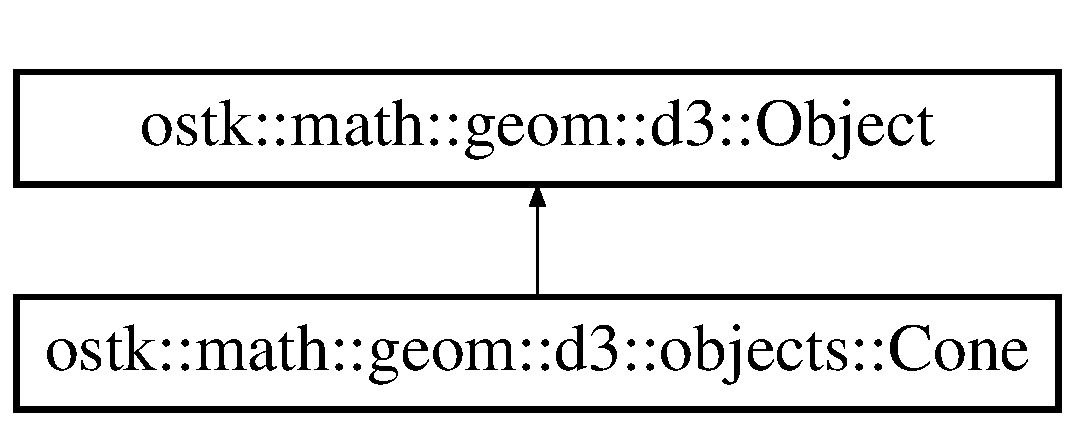
\includegraphics[height=2.000000cm]{classostk_1_1math_1_1geom_1_1d3_1_1objects_1_1_cone}
\end{center}
\end{figure}
\subsection*{Public Member Functions}
\begin{DoxyCompactItemize}
\item 
\hyperlink{classostk_1_1math_1_1geom_1_1d3_1_1objects_1_1_cone_ac86773a78cf513900e8b0d3a2709bfcb}{Cone} (const \hyperlink{classostk_1_1math_1_1geom_1_1d3_1_1objects_1_1_point}{Point} \&an\+Apex, const Vector3d \&an\+Axis, const \hyperlink{classostk_1_1math_1_1geom_1_1_angle}{Angle} \&an\+Angle)
\begin{DoxyCompactList}\small\item\em Constructor. \end{DoxyCompactList}\item 
virtual \hyperlink{classostk_1_1math_1_1geom_1_1d3_1_1objects_1_1_cone}{Cone} $\ast$ \hyperlink{classostk_1_1math_1_1geom_1_1d3_1_1objects_1_1_cone_a656d9720f23ab4e04bbb87dc85f9585a}{clone} () const override
\begin{DoxyCompactList}\small\item\em Clone cone. \end{DoxyCompactList}\item 
bool \hyperlink{classostk_1_1math_1_1geom_1_1d3_1_1objects_1_1_cone_a705e91fbd024f12e214030fd3a4ad8a0}{operator==} (const \hyperlink{classostk_1_1math_1_1geom_1_1d3_1_1objects_1_1_cone}{Cone} \&a\+Cone) const
\begin{DoxyCompactList}\small\item\em Equal to operator. \end{DoxyCompactList}\item 
bool \hyperlink{classostk_1_1math_1_1geom_1_1d3_1_1objects_1_1_cone_abdc26e7cac7c112933e7aab3acc1fc55}{operator!=} (const \hyperlink{classostk_1_1math_1_1geom_1_1d3_1_1objects_1_1_cone}{Cone} \&a\+Cone) const
\begin{DoxyCompactList}\small\item\em Not equal to operator. \end{DoxyCompactList}\item 
virtual bool \hyperlink{classostk_1_1math_1_1geom_1_1d3_1_1objects_1_1_cone_a16491ea1637cf69ad002f59bd2b83553}{is\+Defined} () const override
\begin{DoxyCompactList}\small\item\em Check if cone is defined. \end{DoxyCompactList}\item 
bool \hyperlink{classostk_1_1math_1_1geom_1_1d3_1_1objects_1_1_cone_a3a14e2f8f94a63eecfdce6dfabb26c14}{intersects} (const \hyperlink{classostk_1_1math_1_1geom_1_1d3_1_1objects_1_1_sphere}{Sphere} \&a\+Sphere, const Size a\+Discretization\+Level=\hyperlink{_pyramid_8hpp_a3eb9931e85ba4c9718113211e549e91d}{D\+E\+F\+A\+U\+L\+T\+\_\+\+D\+I\+S\+C\+R\+E\+T\+I\+Z\+A\+T\+I\+O\+N\+\_\+\+L\+E\+V\+EL}) const
\begin{DoxyCompactList}\small\item\em Check if cone intersects sphere. \end{DoxyCompactList}\item 
bool \hyperlink{classostk_1_1math_1_1geom_1_1d3_1_1objects_1_1_cone_a18180f9cf2ee2ec6ef37b478c16a55b4}{intersects} (const \hyperlink{classostk_1_1math_1_1geom_1_1d3_1_1objects_1_1_ellipsoid}{Ellipsoid} \&an\+Ellipsoid, const Size a\+Discretization\+Level=\hyperlink{_pyramid_8hpp_a3eb9931e85ba4c9718113211e549e91d}{D\+E\+F\+A\+U\+L\+T\+\_\+\+D\+I\+S\+C\+R\+E\+T\+I\+Z\+A\+T\+I\+O\+N\+\_\+\+L\+E\+V\+EL}) const
\begin{DoxyCompactList}\small\item\em Check if cone intersects ellipsoid. \end{DoxyCompactList}\item 
\hyperlink{classostk_1_1math_1_1geom_1_1d3_1_1objects_1_1_point}{Point} \hyperlink{classostk_1_1math_1_1geom_1_1d3_1_1objects_1_1_cone_acc452d4c78df49bf3f15c840d6e15c1f}{get\+Apex} () const
\begin{DoxyCompactList}\small\item\em Get cone apex. \end{DoxyCompactList}\item 
Vector3d \hyperlink{classostk_1_1math_1_1geom_1_1d3_1_1objects_1_1_cone_a061a6572fea78dcd22b4466a57bd1b6b}{get\+Axis} () const
\begin{DoxyCompactList}\small\item\em Get cone axis. \end{DoxyCompactList}\item 
\hyperlink{classostk_1_1math_1_1geom_1_1_angle}{Angle} \hyperlink{classostk_1_1math_1_1geom_1_1d3_1_1objects_1_1_cone_ac288545383fe1514951ce13f1e7611f3}{get\+Angle} () const
\begin{DoxyCompactList}\small\item\em Get cone angle. \end{DoxyCompactList}\item 
Array$<$ \hyperlink{classostk_1_1math_1_1geom_1_1d3_1_1objects_1_1_ray}{Ray} $>$ \hyperlink{classostk_1_1math_1_1geom_1_1d3_1_1objects_1_1_cone_a8dc14bb0164c5bf0b2525aaa4c52ea5a}{get\+Rays\+Of\+Lateral\+Surface} (const Size a\+Ray\+Count=\hyperlink{_cone_8hpp_a95759f940e1d5e70e977d66fa8fcb5ec}{D\+E\+F\+A\+U\+L\+T\+\_\+\+R\+A\+Y\+\_\+\+C\+O\+U\+NT}) const
\begin{DoxyCompactList}\small\item\em Get rays of lateral surface. \end{DoxyCompactList}\item 
\hyperlink{classostk_1_1math_1_1geom_1_1d3_1_1_intersection}{Intersection} \hyperlink{classostk_1_1math_1_1geom_1_1d3_1_1objects_1_1_cone_a28ee89d65bf8a7d03b28c48af68243ad}{intersection\+With} (const \hyperlink{classostk_1_1math_1_1geom_1_1d3_1_1objects_1_1_sphere}{Sphere} \&a\+Sphere, const bool only\+In\+Sight=false, const Size a\+Discretization\+Level=\hyperlink{_pyramid_8hpp_a3eb9931e85ba4c9718113211e549e91d}{D\+E\+F\+A\+U\+L\+T\+\_\+\+D\+I\+S\+C\+R\+E\+T\+I\+Z\+A\+T\+I\+O\+N\+\_\+\+L\+E\+V\+EL}) const
\begin{DoxyCompactList}\small\item\em Compute intersection of cone with sphere. \end{DoxyCompactList}\item 
\hyperlink{classostk_1_1math_1_1geom_1_1d3_1_1_intersection}{Intersection} \hyperlink{classostk_1_1math_1_1geom_1_1d3_1_1objects_1_1_cone_ac47f327abb71af922d824beca7af0c62}{intersection\+With} (const \hyperlink{classostk_1_1math_1_1geom_1_1d3_1_1objects_1_1_ellipsoid}{Ellipsoid} \&an\+Ellipsoid, const bool only\+In\+Sight=false, const Size a\+Discretization\+Level=\hyperlink{_pyramid_8hpp_a3eb9931e85ba4c9718113211e549e91d}{D\+E\+F\+A\+U\+L\+T\+\_\+\+D\+I\+S\+C\+R\+E\+T\+I\+Z\+A\+T\+I\+O\+N\+\_\+\+L\+E\+V\+EL}) const
\begin{DoxyCompactList}\small\item\em Compute intersection of cone with ellipsoid. \end{DoxyCompactList}\item 
virtual void \hyperlink{classostk_1_1math_1_1geom_1_1d3_1_1objects_1_1_cone_a511e3f582e15b11f9b571ec199fdf707}{print} (std\+::ostream \&an\+Output\+Stream, bool display\+Decorators=true) const override
\begin{DoxyCompactList}\small\item\em Print cone. \end{DoxyCompactList}\item 
virtual void \hyperlink{classostk_1_1math_1_1geom_1_1d3_1_1objects_1_1_cone_a9b783e16344d65dfba68c63d1adca3e1}{apply\+Transformation} (const \hyperlink{classostk_1_1math_1_1geom_1_1d3_1_1_transformation}{Transformation} \&a\+Transformation) override
\begin{DoxyCompactList}\small\item\em Apply transformation to cone. \end{DoxyCompactList}\end{DoxyCompactItemize}
\subsection*{Static Public Member Functions}
\begin{DoxyCompactItemize}
\item 
static \hyperlink{classostk_1_1math_1_1geom_1_1d3_1_1objects_1_1_cone}{Cone} \hyperlink{classostk_1_1math_1_1geom_1_1d3_1_1objects_1_1_cone_a06438bb2e619615fcbbce8097186edbe}{Undefined} ()
\begin{DoxyCompactList}\small\item\em Constructs an undefined cone. \end{DoxyCompactList}\end{DoxyCompactItemize}


\subsection{Detailed Description}
\hyperlink{classostk_1_1math_1_1geom_1_1d3_1_1objects_1_1_cone}{Cone}. 

A cone is a three-\/dimensional geometric shape that tapers smoothly from a flat circular base to a point called the apex.

https\+://en.wikipedia.\+org/wiki/\+Cone 

\subsection{Constructor \& Destructor Documentation}
\mbox{\Hypertarget{classostk_1_1math_1_1geom_1_1d3_1_1objects_1_1_cone_ac86773a78cf513900e8b0d3a2709bfcb}\label{classostk_1_1math_1_1geom_1_1d3_1_1objects_1_1_cone_ac86773a78cf513900e8b0d3a2709bfcb}} 
\index{ostk\+::math\+::geom\+::d3\+::objects\+::\+Cone@{ostk\+::math\+::geom\+::d3\+::objects\+::\+Cone}!Cone@{Cone}}
\index{Cone@{Cone}!ostk\+::math\+::geom\+::d3\+::objects\+::\+Cone@{ostk\+::math\+::geom\+::d3\+::objects\+::\+Cone}}
\subsubsection{\texorpdfstring{Cone()}{Cone()}}
{\footnotesize\ttfamily ostk\+::math\+::geom\+::d3\+::objects\+::\+Cone\+::\+Cone (\begin{DoxyParamCaption}\item[{const \hyperlink{classostk_1_1math_1_1geom_1_1d3_1_1objects_1_1_point}{Point} \&}]{an\+Apex,  }\item[{const Vector3d \&}]{an\+Axis,  }\item[{const \hyperlink{classostk_1_1math_1_1geom_1_1_angle}{Angle} \&}]{an\+Angle }\end{DoxyParamCaption})}



Constructor. 


\begin{DoxyCode}
Point apex = \{ 0.0, 0.0, 0.0 \} ;
\hyperlink{namespaceostk_1_1math_1_1obj_a18744cbf433bce59f6758d9fe3b1dff1}{Vector3d} axis = \{ 0.0, 0.0, 1.0 \} ;
Angle angle = \hyperlink{classostk_1_1math_1_1geom_1_1_angle_a2cefda601167af07f61f0477776203ca}{Angle::Degrees}(15.0) ;
\hyperlink{classostk_1_1math_1_1geom_1_1d3_1_1objects_1_1_cone_ac86773a78cf513900e8b0d3a2709bfcb}{Cone} cone = \{ apex, axis, angle \} ;
\end{DoxyCode}



\begin{DoxyParams}[1]{Parameters}
\mbox{\tt in}  & {\em an\+Apex} & A cone apex \\
\hline
\mbox{\tt in}  & {\em an\+Axis} & A cone axis \\
\hline
\mbox{\tt in}  & {\em an\+Angle} & A cone angle \\
\hline
\end{DoxyParams}


\subsection{Member Function Documentation}
\mbox{\Hypertarget{classostk_1_1math_1_1geom_1_1d3_1_1objects_1_1_cone_a9b783e16344d65dfba68c63d1adca3e1}\label{classostk_1_1math_1_1geom_1_1d3_1_1objects_1_1_cone_a9b783e16344d65dfba68c63d1adca3e1}} 
\index{ostk\+::math\+::geom\+::d3\+::objects\+::\+Cone@{ostk\+::math\+::geom\+::d3\+::objects\+::\+Cone}!apply\+Transformation@{apply\+Transformation}}
\index{apply\+Transformation@{apply\+Transformation}!ostk\+::math\+::geom\+::d3\+::objects\+::\+Cone@{ostk\+::math\+::geom\+::d3\+::objects\+::\+Cone}}
\subsubsection{\texorpdfstring{apply\+Transformation()}{applyTransformation()}}
{\footnotesize\ttfamily void ostk\+::math\+::geom\+::d3\+::objects\+::\+Cone\+::apply\+Transformation (\begin{DoxyParamCaption}\item[{const \hyperlink{classostk_1_1math_1_1geom_1_1d3_1_1_transformation}{Transformation} \&}]{a\+Transformation }\end{DoxyParamCaption})\hspace{0.3cm}{\ttfamily [override]}, {\ttfamily [virtual]}}



Apply transformation to cone. 


\begin{DoxyParams}[1]{Parameters}
\mbox{\tt in}  & {\em a\+Transformation} & A transformation \\
\hline
\end{DoxyParams}


Implements \hyperlink{classostk_1_1math_1_1geom_1_1d3_1_1_object_ae9194dd6d2bb4df09292ffc84dccdb1d}{ostk\+::math\+::geom\+::d3\+::\+Object}.

\mbox{\Hypertarget{classostk_1_1math_1_1geom_1_1d3_1_1objects_1_1_cone_a656d9720f23ab4e04bbb87dc85f9585a}\label{classostk_1_1math_1_1geom_1_1d3_1_1objects_1_1_cone_a656d9720f23ab4e04bbb87dc85f9585a}} 
\index{ostk\+::math\+::geom\+::d3\+::objects\+::\+Cone@{ostk\+::math\+::geom\+::d3\+::objects\+::\+Cone}!clone@{clone}}
\index{clone@{clone}!ostk\+::math\+::geom\+::d3\+::objects\+::\+Cone@{ostk\+::math\+::geom\+::d3\+::objects\+::\+Cone}}
\subsubsection{\texorpdfstring{clone()}{clone()}}
{\footnotesize\ttfamily \hyperlink{classostk_1_1math_1_1geom_1_1d3_1_1objects_1_1_cone}{Cone} $\ast$ ostk\+::math\+::geom\+::d3\+::objects\+::\+Cone\+::clone (\begin{DoxyParamCaption}{ }\end{DoxyParamCaption}) const\hspace{0.3cm}{\ttfamily [override]}, {\ttfamily [virtual]}}



Clone cone. 

\begin{DoxyReturn}{Returns}
Pointer to cloned cone 
\end{DoxyReturn}


Implements \hyperlink{classostk_1_1math_1_1geom_1_1d3_1_1_object_a676013f9555f6492687f9809b2db887b}{ostk\+::math\+::geom\+::d3\+::\+Object}.

\mbox{\Hypertarget{classostk_1_1math_1_1geom_1_1d3_1_1objects_1_1_cone_ac288545383fe1514951ce13f1e7611f3}\label{classostk_1_1math_1_1geom_1_1d3_1_1objects_1_1_cone_ac288545383fe1514951ce13f1e7611f3}} 
\index{ostk\+::math\+::geom\+::d3\+::objects\+::\+Cone@{ostk\+::math\+::geom\+::d3\+::objects\+::\+Cone}!get\+Angle@{get\+Angle}}
\index{get\+Angle@{get\+Angle}!ostk\+::math\+::geom\+::d3\+::objects\+::\+Cone@{ostk\+::math\+::geom\+::d3\+::objects\+::\+Cone}}
\subsubsection{\texorpdfstring{get\+Angle()}{getAngle()}}
{\footnotesize\ttfamily \hyperlink{classostk_1_1math_1_1geom_1_1_angle}{Angle} ostk\+::math\+::geom\+::d3\+::objects\+::\+Cone\+::get\+Angle (\begin{DoxyParamCaption}{ }\end{DoxyParamCaption}) const}



Get cone angle. 

\begin{DoxyReturn}{Returns}
\hyperlink{classostk_1_1math_1_1geom_1_1d3_1_1objects_1_1_cone}{Cone} angle 
\end{DoxyReturn}
\mbox{\Hypertarget{classostk_1_1math_1_1geom_1_1d3_1_1objects_1_1_cone_acc452d4c78df49bf3f15c840d6e15c1f}\label{classostk_1_1math_1_1geom_1_1d3_1_1objects_1_1_cone_acc452d4c78df49bf3f15c840d6e15c1f}} 
\index{ostk\+::math\+::geom\+::d3\+::objects\+::\+Cone@{ostk\+::math\+::geom\+::d3\+::objects\+::\+Cone}!get\+Apex@{get\+Apex}}
\index{get\+Apex@{get\+Apex}!ostk\+::math\+::geom\+::d3\+::objects\+::\+Cone@{ostk\+::math\+::geom\+::d3\+::objects\+::\+Cone}}
\subsubsection{\texorpdfstring{get\+Apex()}{getApex()}}
{\footnotesize\ttfamily \hyperlink{classostk_1_1math_1_1geom_1_1d3_1_1objects_1_1_point}{Point} ostk\+::math\+::geom\+::d3\+::objects\+::\+Cone\+::get\+Apex (\begin{DoxyParamCaption}{ }\end{DoxyParamCaption}) const}



Get cone apex. 

\begin{DoxyReturn}{Returns}
\hyperlink{classostk_1_1math_1_1geom_1_1d3_1_1objects_1_1_cone}{Cone} apex 
\end{DoxyReturn}
\mbox{\Hypertarget{classostk_1_1math_1_1geom_1_1d3_1_1objects_1_1_cone_a061a6572fea78dcd22b4466a57bd1b6b}\label{classostk_1_1math_1_1geom_1_1d3_1_1objects_1_1_cone_a061a6572fea78dcd22b4466a57bd1b6b}} 
\index{ostk\+::math\+::geom\+::d3\+::objects\+::\+Cone@{ostk\+::math\+::geom\+::d3\+::objects\+::\+Cone}!get\+Axis@{get\+Axis}}
\index{get\+Axis@{get\+Axis}!ostk\+::math\+::geom\+::d3\+::objects\+::\+Cone@{ostk\+::math\+::geom\+::d3\+::objects\+::\+Cone}}
\subsubsection{\texorpdfstring{get\+Axis()}{getAxis()}}
{\footnotesize\ttfamily Vector3d ostk\+::math\+::geom\+::d3\+::objects\+::\+Cone\+::get\+Axis (\begin{DoxyParamCaption}{ }\end{DoxyParamCaption}) const}



Get cone axis. 

\begin{DoxyReturn}{Returns}
\hyperlink{classostk_1_1math_1_1geom_1_1d3_1_1objects_1_1_cone}{Cone} axis 
\end{DoxyReturn}
\mbox{\Hypertarget{classostk_1_1math_1_1geom_1_1d3_1_1objects_1_1_cone_a8dc14bb0164c5bf0b2525aaa4c52ea5a}\label{classostk_1_1math_1_1geom_1_1d3_1_1objects_1_1_cone_a8dc14bb0164c5bf0b2525aaa4c52ea5a}} 
\index{ostk\+::math\+::geom\+::d3\+::objects\+::\+Cone@{ostk\+::math\+::geom\+::d3\+::objects\+::\+Cone}!get\+Rays\+Of\+Lateral\+Surface@{get\+Rays\+Of\+Lateral\+Surface}}
\index{get\+Rays\+Of\+Lateral\+Surface@{get\+Rays\+Of\+Lateral\+Surface}!ostk\+::math\+::geom\+::d3\+::objects\+::\+Cone@{ostk\+::math\+::geom\+::d3\+::objects\+::\+Cone}}
\subsubsection{\texorpdfstring{get\+Rays\+Of\+Lateral\+Surface()}{getRaysOfLateralSurface()}}
{\footnotesize\ttfamily Array$<$ \hyperlink{classostk_1_1math_1_1geom_1_1d3_1_1objects_1_1_ray}{Ray} $>$ ostk\+::math\+::geom\+::d3\+::objects\+::\+Cone\+::get\+Rays\+Of\+Lateral\+Surface (\begin{DoxyParamCaption}\item[{const Size}]{a\+Ray\+Count = {\ttfamily \hyperlink{_cone_8hpp_a95759f940e1d5e70e977d66fa8fcb5ec}{D\+E\+F\+A\+U\+L\+T\+\_\+\+R\+A\+Y\+\_\+\+C\+O\+U\+NT}} }\end{DoxyParamCaption}) const}



Get rays of lateral surface. 


\begin{DoxyParams}[1]{Parameters}
\mbox{\tt in}  & {\em a\+Ray\+Count} & A number of rays (at least face count) \\
\hline
\end{DoxyParams}
\begin{DoxyReturn}{Returns}
Array of rays 
\end{DoxyReturn}
\mbox{\Hypertarget{classostk_1_1math_1_1geom_1_1d3_1_1objects_1_1_cone_a28ee89d65bf8a7d03b28c48af68243ad}\label{classostk_1_1math_1_1geom_1_1d3_1_1objects_1_1_cone_a28ee89d65bf8a7d03b28c48af68243ad}} 
\index{ostk\+::math\+::geom\+::d3\+::objects\+::\+Cone@{ostk\+::math\+::geom\+::d3\+::objects\+::\+Cone}!intersection\+With@{intersection\+With}}
\index{intersection\+With@{intersection\+With}!ostk\+::math\+::geom\+::d3\+::objects\+::\+Cone@{ostk\+::math\+::geom\+::d3\+::objects\+::\+Cone}}
\subsubsection{\texorpdfstring{intersection\+With()}{intersectionWith()}\hspace{0.1cm}{\footnotesize\ttfamily [1/2]}}
{\footnotesize\ttfamily \hyperlink{classostk_1_1math_1_1geom_1_1d3_1_1_intersection}{Intersection} ostk\+::math\+::geom\+::d3\+::objects\+::\+Cone\+::intersection\+With (\begin{DoxyParamCaption}\item[{const \hyperlink{classostk_1_1math_1_1geom_1_1d3_1_1objects_1_1_sphere}{Sphere} \&}]{a\+Sphere,  }\item[{const bool}]{only\+In\+Sight = {\ttfamily false},  }\item[{const Size}]{a\+Discretization\+Level = {\ttfamily \hyperlink{_pyramid_8hpp_a3eb9931e85ba4c9718113211e549e91d}{D\+E\+F\+A\+U\+L\+T\+\_\+\+D\+I\+S\+C\+R\+E\+T\+I\+Z\+A\+T\+I\+O\+N\+\_\+\+L\+E\+V\+EL}} }\end{DoxyParamCaption}) const}



Compute intersection of cone with sphere. 


\begin{DoxyParams}[1]{Parameters}
\mbox{\tt in}  & {\em a\+Sphere} & A sphere \\
\hline
\mbox{\tt in}  & {\em only\+In\+Sight} & (optional) If true, only return intersection points that are in sight \\
\hline
\mbox{\tt in}  & {\em a\+Discretization\+Level} & (optional) The polygonal discretization level \\
\hline
\end{DoxyParams}
\begin{DoxyReturn}{Returns}
\hyperlink{classostk_1_1math_1_1geom_1_1d3_1_1_intersection}{Intersection} of cone with sphere 
\end{DoxyReturn}
\mbox{\Hypertarget{classostk_1_1math_1_1geom_1_1d3_1_1objects_1_1_cone_ac47f327abb71af922d824beca7af0c62}\label{classostk_1_1math_1_1geom_1_1d3_1_1objects_1_1_cone_ac47f327abb71af922d824beca7af0c62}} 
\index{ostk\+::math\+::geom\+::d3\+::objects\+::\+Cone@{ostk\+::math\+::geom\+::d3\+::objects\+::\+Cone}!intersection\+With@{intersection\+With}}
\index{intersection\+With@{intersection\+With}!ostk\+::math\+::geom\+::d3\+::objects\+::\+Cone@{ostk\+::math\+::geom\+::d3\+::objects\+::\+Cone}}
\subsubsection{\texorpdfstring{intersection\+With()}{intersectionWith()}\hspace{0.1cm}{\footnotesize\ttfamily [2/2]}}
{\footnotesize\ttfamily \hyperlink{classostk_1_1math_1_1geom_1_1d3_1_1_intersection}{Intersection} ostk\+::math\+::geom\+::d3\+::objects\+::\+Cone\+::intersection\+With (\begin{DoxyParamCaption}\item[{const \hyperlink{classostk_1_1math_1_1geom_1_1d3_1_1objects_1_1_ellipsoid}{Ellipsoid} \&}]{an\+Ellipsoid,  }\item[{const bool}]{only\+In\+Sight = {\ttfamily false},  }\item[{const Size}]{a\+Discretization\+Level = {\ttfamily \hyperlink{_pyramid_8hpp_a3eb9931e85ba4c9718113211e549e91d}{D\+E\+F\+A\+U\+L\+T\+\_\+\+D\+I\+S\+C\+R\+E\+T\+I\+Z\+A\+T\+I\+O\+N\+\_\+\+L\+E\+V\+EL}} }\end{DoxyParamCaption}) const}



Compute intersection of cone with ellipsoid. 


\begin{DoxyParams}[1]{Parameters}
\mbox{\tt in}  & {\em an\+Ellipsoid} & An ellipsoid \\
\hline
\mbox{\tt in}  & {\em only\+In\+Sight} & (optional) If true, only return intersection points that are in sight \\
\hline
\mbox{\tt in}  & {\em a\+Discretization\+Level} & (optional) The polygonal discretization level \\
\hline
\end{DoxyParams}
\begin{DoxyReturn}{Returns}
\hyperlink{classostk_1_1math_1_1geom_1_1d3_1_1_intersection}{Intersection} of cone with ellipsoid 
\end{DoxyReturn}
\mbox{\Hypertarget{classostk_1_1math_1_1geom_1_1d3_1_1objects_1_1_cone_a3a14e2f8f94a63eecfdce6dfabb26c14}\label{classostk_1_1math_1_1geom_1_1d3_1_1objects_1_1_cone_a3a14e2f8f94a63eecfdce6dfabb26c14}} 
\index{ostk\+::math\+::geom\+::d3\+::objects\+::\+Cone@{ostk\+::math\+::geom\+::d3\+::objects\+::\+Cone}!intersects@{intersects}}
\index{intersects@{intersects}!ostk\+::math\+::geom\+::d3\+::objects\+::\+Cone@{ostk\+::math\+::geom\+::d3\+::objects\+::\+Cone}}
\subsubsection{\texorpdfstring{intersects()}{intersects()}\hspace{0.1cm}{\footnotesize\ttfamily [1/2]}}
{\footnotesize\ttfamily bool ostk\+::math\+::geom\+::d3\+::objects\+::\+Cone\+::intersects (\begin{DoxyParamCaption}\item[{const \hyperlink{classostk_1_1math_1_1geom_1_1d3_1_1objects_1_1_sphere}{Sphere} \&}]{a\+Sphere,  }\item[{const Size}]{a\+Discretization\+Level = {\ttfamily \hyperlink{_pyramid_8hpp_a3eb9931e85ba4c9718113211e549e91d}{D\+E\+F\+A\+U\+L\+T\+\_\+\+D\+I\+S\+C\+R\+E\+T\+I\+Z\+A\+T\+I\+O\+N\+\_\+\+L\+E\+V\+EL}} }\end{DoxyParamCaption}) const}



Check if cone intersects sphere. 


\begin{DoxyCode}
\hyperlink{classostk_1_1math_1_1geom_1_1d3_1_1objects_1_1_cone_ac86773a78cf513900e8b0d3a2709bfcb}{Cone} cone = ... ;
Sphere sphere = ... ;
cone.intersects(sphere) ;
\end{DoxyCode}



\begin{DoxyParams}[1]{Parameters}
\mbox{\tt in}  & {\em a\+Sphere} & A sphere \\
\hline
\mbox{\tt in}  & {\em a\+Discretization\+Level} & (optional) The polygonal discretization level \\
\hline
\end{DoxyParams}
\begin{DoxyReturn}{Returns}
True if cone intersects sphere 
\end{DoxyReturn}
\mbox{\Hypertarget{classostk_1_1math_1_1geom_1_1d3_1_1objects_1_1_cone_a18180f9cf2ee2ec6ef37b478c16a55b4}\label{classostk_1_1math_1_1geom_1_1d3_1_1objects_1_1_cone_a18180f9cf2ee2ec6ef37b478c16a55b4}} 
\index{ostk\+::math\+::geom\+::d3\+::objects\+::\+Cone@{ostk\+::math\+::geom\+::d3\+::objects\+::\+Cone}!intersects@{intersects}}
\index{intersects@{intersects}!ostk\+::math\+::geom\+::d3\+::objects\+::\+Cone@{ostk\+::math\+::geom\+::d3\+::objects\+::\+Cone}}
\subsubsection{\texorpdfstring{intersects()}{intersects()}\hspace{0.1cm}{\footnotesize\ttfamily [2/2]}}
{\footnotesize\ttfamily bool ostk\+::math\+::geom\+::d3\+::objects\+::\+Cone\+::intersects (\begin{DoxyParamCaption}\item[{const \hyperlink{classostk_1_1math_1_1geom_1_1d3_1_1objects_1_1_ellipsoid}{Ellipsoid} \&}]{an\+Ellipsoid,  }\item[{const Size}]{a\+Discretization\+Level = {\ttfamily \hyperlink{_pyramid_8hpp_a3eb9931e85ba4c9718113211e549e91d}{D\+E\+F\+A\+U\+L\+T\+\_\+\+D\+I\+S\+C\+R\+E\+T\+I\+Z\+A\+T\+I\+O\+N\+\_\+\+L\+E\+V\+EL}} }\end{DoxyParamCaption}) const}



Check if cone intersects ellipsoid. 


\begin{DoxyCode}
\hyperlink{classostk_1_1math_1_1geom_1_1d3_1_1objects_1_1_cone_ac86773a78cf513900e8b0d3a2709bfcb}{Cone} cone = ... ;
Ellipsoid ellipsoid = ... ;
cone.intersects(ellipsoid) ;
\end{DoxyCode}



\begin{DoxyParams}[1]{Parameters}
\mbox{\tt in}  & {\em an\+Ellipsoid} & An ellipsoid \\
\hline
\mbox{\tt in}  & {\em a\+Discretization\+Level} & (optional) The polygonal discretization level \\
\hline
\end{DoxyParams}
\begin{DoxyReturn}{Returns}
True if cone intersects ellipsoid 
\end{DoxyReturn}
\mbox{\Hypertarget{classostk_1_1math_1_1geom_1_1d3_1_1objects_1_1_cone_a16491ea1637cf69ad002f59bd2b83553}\label{classostk_1_1math_1_1geom_1_1d3_1_1objects_1_1_cone_a16491ea1637cf69ad002f59bd2b83553}} 
\index{ostk\+::math\+::geom\+::d3\+::objects\+::\+Cone@{ostk\+::math\+::geom\+::d3\+::objects\+::\+Cone}!is\+Defined@{is\+Defined}}
\index{is\+Defined@{is\+Defined}!ostk\+::math\+::geom\+::d3\+::objects\+::\+Cone@{ostk\+::math\+::geom\+::d3\+::objects\+::\+Cone}}
\subsubsection{\texorpdfstring{is\+Defined()}{isDefined()}}
{\footnotesize\ttfamily bool ostk\+::math\+::geom\+::d3\+::objects\+::\+Cone\+::is\+Defined (\begin{DoxyParamCaption}{ }\end{DoxyParamCaption}) const\hspace{0.3cm}{\ttfamily [override]}, {\ttfamily [virtual]}}



Check if cone is defined. 

\begin{DoxyReturn}{Returns}
True if cone is defined 
\end{DoxyReturn}


Implements \hyperlink{classostk_1_1math_1_1geom_1_1d3_1_1_object_a271a1964cd208be85ce9a0a429395ad8}{ostk\+::math\+::geom\+::d3\+::\+Object}.

\mbox{\Hypertarget{classostk_1_1math_1_1geom_1_1d3_1_1objects_1_1_cone_abdc26e7cac7c112933e7aab3acc1fc55}\label{classostk_1_1math_1_1geom_1_1d3_1_1objects_1_1_cone_abdc26e7cac7c112933e7aab3acc1fc55}} 
\index{ostk\+::math\+::geom\+::d3\+::objects\+::\+Cone@{ostk\+::math\+::geom\+::d3\+::objects\+::\+Cone}!operator"!=@{operator"!=}}
\index{operator"!=@{operator"!=}!ostk\+::math\+::geom\+::d3\+::objects\+::\+Cone@{ostk\+::math\+::geom\+::d3\+::objects\+::\+Cone}}
\subsubsection{\texorpdfstring{operator"!=()}{operator!=()}}
{\footnotesize\ttfamily bool ostk\+::math\+::geom\+::d3\+::objects\+::\+Cone\+::operator!= (\begin{DoxyParamCaption}\item[{const \hyperlink{classostk_1_1math_1_1geom_1_1d3_1_1objects_1_1_cone}{Cone} \&}]{a\+Cone }\end{DoxyParamCaption}) const}



Not equal to operator. 


\begin{DoxyParams}[1]{Parameters}
\mbox{\tt in}  & {\em a\+Cone} & A cone \\
\hline
\end{DoxyParams}
\begin{DoxyReturn}{Returns}
True if cones are not equal 
\end{DoxyReturn}
\mbox{\Hypertarget{classostk_1_1math_1_1geom_1_1d3_1_1objects_1_1_cone_a705e91fbd024f12e214030fd3a4ad8a0}\label{classostk_1_1math_1_1geom_1_1d3_1_1objects_1_1_cone_a705e91fbd024f12e214030fd3a4ad8a0}} 
\index{ostk\+::math\+::geom\+::d3\+::objects\+::\+Cone@{ostk\+::math\+::geom\+::d3\+::objects\+::\+Cone}!operator==@{operator==}}
\index{operator==@{operator==}!ostk\+::math\+::geom\+::d3\+::objects\+::\+Cone@{ostk\+::math\+::geom\+::d3\+::objects\+::\+Cone}}
\subsubsection{\texorpdfstring{operator==()}{operator==()}}
{\footnotesize\ttfamily bool ostk\+::math\+::geom\+::d3\+::objects\+::\+Cone\+::operator== (\begin{DoxyParamCaption}\item[{const \hyperlink{classostk_1_1math_1_1geom_1_1d3_1_1objects_1_1_cone}{Cone} \&}]{a\+Cone }\end{DoxyParamCaption}) const}



Equal to operator. 


\begin{DoxyParams}[1]{Parameters}
\mbox{\tt in}  & {\em a\+Cone} & A cone \\
\hline
\end{DoxyParams}
\begin{DoxyReturn}{Returns}
True if cones are equal 
\end{DoxyReturn}
\mbox{\Hypertarget{classostk_1_1math_1_1geom_1_1d3_1_1objects_1_1_cone_a511e3f582e15b11f9b571ec199fdf707}\label{classostk_1_1math_1_1geom_1_1d3_1_1objects_1_1_cone_a511e3f582e15b11f9b571ec199fdf707}} 
\index{ostk\+::math\+::geom\+::d3\+::objects\+::\+Cone@{ostk\+::math\+::geom\+::d3\+::objects\+::\+Cone}!print@{print}}
\index{print@{print}!ostk\+::math\+::geom\+::d3\+::objects\+::\+Cone@{ostk\+::math\+::geom\+::d3\+::objects\+::\+Cone}}
\subsubsection{\texorpdfstring{print()}{print()}}
{\footnotesize\ttfamily void ostk\+::math\+::geom\+::d3\+::objects\+::\+Cone\+::print (\begin{DoxyParamCaption}\item[{std\+::ostream \&}]{an\+Output\+Stream,  }\item[{bool}]{display\+Decorators = {\ttfamily true} }\end{DoxyParamCaption}) const\hspace{0.3cm}{\ttfamily [override]}, {\ttfamily [virtual]}}



Print cone. 


\begin{DoxyParams}[1]{Parameters}
\mbox{\tt in}  & {\em an\+Output\+Stream} & An output stream \\
\hline
\mbox{\tt in}  & {\em (optional)} & display\+Decorators If true, display decorators \\
\hline
\end{DoxyParams}


Implements \hyperlink{classostk_1_1math_1_1geom_1_1d3_1_1_object_ab2a2a782503b97d1cecabdfedc636fce}{ostk\+::math\+::geom\+::d3\+::\+Object}.

\mbox{\Hypertarget{classostk_1_1math_1_1geom_1_1d3_1_1objects_1_1_cone_a06438bb2e619615fcbbce8097186edbe}\label{classostk_1_1math_1_1geom_1_1d3_1_1objects_1_1_cone_a06438bb2e619615fcbbce8097186edbe}} 
\index{ostk\+::math\+::geom\+::d3\+::objects\+::\+Cone@{ostk\+::math\+::geom\+::d3\+::objects\+::\+Cone}!Undefined@{Undefined}}
\index{Undefined@{Undefined}!ostk\+::math\+::geom\+::d3\+::objects\+::\+Cone@{ostk\+::math\+::geom\+::d3\+::objects\+::\+Cone}}
\subsubsection{\texorpdfstring{Undefined()}{Undefined()}}
{\footnotesize\ttfamily \hyperlink{classostk_1_1math_1_1geom_1_1d3_1_1objects_1_1_cone}{Cone} ostk\+::math\+::geom\+::d3\+::objects\+::\+Cone\+::\+Undefined (\begin{DoxyParamCaption}{ }\end{DoxyParamCaption})\hspace{0.3cm}{\ttfamily [static]}}



Constructs an undefined cone. 

\begin{DoxyReturn}{Returns}
Undefined cone 
\end{DoxyReturn}


The documentation for this class was generated from the following files\+:\begin{DoxyCompactItemize}
\item 
include/\+Open\+Space\+Toolkit/\+Mathematics/\+Geometry/3\+D/\+Objects/\hyperlink{_cone_8hpp}{Cone.\+hpp}\item 
src/\+Open\+Space\+Toolkit/\+Mathematics/\+Geometry/3\+D/\+Objects/\hyperlink{_cone_8cpp}{Cone.\+cpp}\end{DoxyCompactItemize}

\hypertarget{classostk_1_1math_1_1geom_1_1d3_1_1objects_1_1_cuboid}{}\doxysection{ostk\+::math\+::geom\+::d3\+::objects\+::Cuboid Class Reference}
\label{classostk_1_1math_1_1geom_1_1d3_1_1objects_1_1_cuboid}\index{ostk::math::geom::d3::objects::Cuboid@{ostk::math::geom::d3::objects::Cuboid}}


\mbox{\hyperlink{classostk_1_1math_1_1geom_1_1d3_1_1objects_1_1_cuboid}{Cuboid}}.  




{\ttfamily \#include $<$Cuboid.\+hpp$>$}

Inheritance diagram for ostk\+::math\+::geom\+::d3\+::objects\+::Cuboid\+:\begin{figure}[H]
\begin{center}
\leavevmode
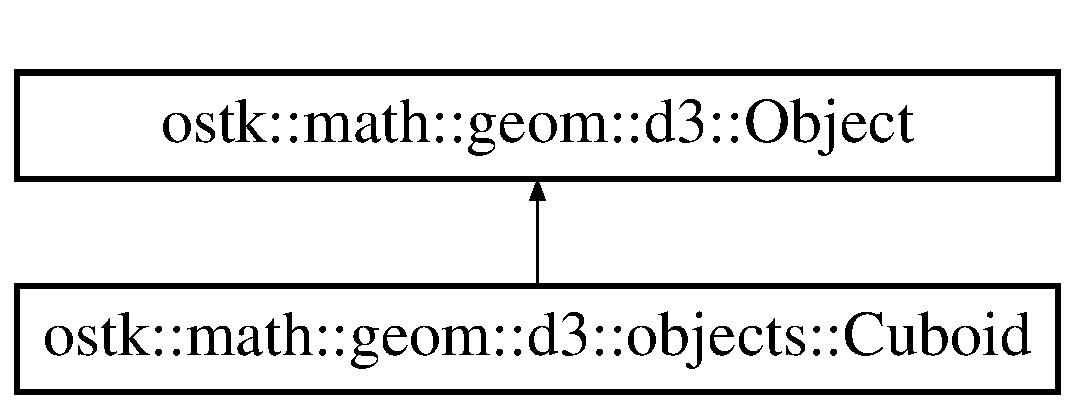
\includegraphics[height=2.000000cm]{classostk_1_1math_1_1geom_1_1d3_1_1objects_1_1_cuboid}
\end{center}
\end{figure}
\doxysubsection*{Public Types}
\begin{DoxyCompactItemize}
\item 
typedef \mbox{\hyperlink{classostk_1_1math_1_1geom_1_1d3_1_1objects_1_1_point}{Point}} \mbox{\hyperlink{classostk_1_1math_1_1geom_1_1d3_1_1objects_1_1_cuboid_a0d3440e0c30348ece10f3658130e9b55}{Vertex}}
\item 
typedef \mbox{\hyperlink{classostk_1_1math_1_1geom_1_1d3_1_1objects_1_1_segment}{Segment}} \mbox{\hyperlink{classostk_1_1math_1_1geom_1_1d3_1_1objects_1_1_cuboid_af9482cb1219e7d447aaf76b6e2dbb1d1}{Edge}}
\end{DoxyCompactItemize}
\doxysubsection*{Public Member Functions}
\begin{DoxyCompactItemize}
\item 
\mbox{\hyperlink{classostk_1_1math_1_1geom_1_1d3_1_1objects_1_1_cuboid_a1da071d7cbb0a694348628f098f77c5b}{Cuboid}} (const \mbox{\hyperlink{classostk_1_1math_1_1geom_1_1d3_1_1objects_1_1_point}{Point}} \&a\+Center, const std\+::array$<$ Vector3d, 3 $>$ \&a\+Axis\+Array, const std\+::array$<$ Real, 3 $>$ \&an\+Extent)
\begin{DoxyCompactList}\small\item\em Constructor. \end{DoxyCompactList}\item 
virtual \mbox{\hyperlink{classostk_1_1math_1_1geom_1_1d3_1_1objects_1_1_cuboid}{Cuboid}} $\ast$ \mbox{\hyperlink{classostk_1_1math_1_1geom_1_1d3_1_1objects_1_1_cuboid_a0096ba5626ce44a892f05610f6d6eb13}{clone}} () const override
\begin{DoxyCompactList}\small\item\em Clone cuboid. \end{DoxyCompactList}\item 
bool \mbox{\hyperlink{classostk_1_1math_1_1geom_1_1d3_1_1objects_1_1_cuboid_aeb4eab71c3019aef0ad4e561bcf20f06}{operator==}} (const \mbox{\hyperlink{classostk_1_1math_1_1geom_1_1d3_1_1objects_1_1_cuboid}{Cuboid}} \&a\+Cuboid) const
\begin{DoxyCompactList}\small\item\em Equal to operator. \end{DoxyCompactList}\item 
bool \mbox{\hyperlink{classostk_1_1math_1_1geom_1_1d3_1_1objects_1_1_cuboid_a8517c894a67a923ef2179c3f615e5ef1}{operator!=}} (const \mbox{\hyperlink{classostk_1_1math_1_1geom_1_1d3_1_1objects_1_1_cuboid}{Cuboid}} \&a\+Cuboid) const
\begin{DoxyCompactList}\small\item\em Not equal to operator. \end{DoxyCompactList}\item 
virtual bool \mbox{\hyperlink{classostk_1_1math_1_1geom_1_1d3_1_1objects_1_1_cuboid_a4e7dbaf957b92cbbb02dd85c0b505366}{is\+Defined}} () const override
\begin{DoxyCompactList}\small\item\em Check if cuboid is defined. \end{DoxyCompactList}\item 
bool \mbox{\hyperlink{classostk_1_1math_1_1geom_1_1d3_1_1objects_1_1_cuboid_a4e4bcebf83464e2f946346d606c5f44c}{is\+Near}} (const \mbox{\hyperlink{classostk_1_1math_1_1geom_1_1d3_1_1objects_1_1_cuboid}{Cuboid}} \&a\+Cuboid, const Real \&a\+Tolerance) const
\begin{DoxyCompactList}\small\item\em Check if cuboid is near another cuboid. \end{DoxyCompactList}\item 
bool \mbox{\hyperlink{classostk_1_1math_1_1geom_1_1d3_1_1objects_1_1_cuboid_ae3bd1daf3311571b020da901f24d1a41}{intersects}} (const \mbox{\hyperlink{classostk_1_1math_1_1geom_1_1d3_1_1objects_1_1_point}{Point}} \&a\+Point) const
\begin{DoxyCompactList}\small\item\em Check if cuboid intersects point. \end{DoxyCompactList}\item 
bool \mbox{\hyperlink{classostk_1_1math_1_1geom_1_1d3_1_1objects_1_1_cuboid_aa922a6ee7f3fe7cbbbfe584fa0d86e2c}{intersects}} (const \mbox{\hyperlink{classostk_1_1math_1_1geom_1_1d3_1_1objects_1_1_point_set}{Point\+Set}} \&a\+Point\+Set) const
\begin{DoxyCompactList}\small\item\em Check if cuboid intersects point set. \end{DoxyCompactList}\item 
bool \mbox{\hyperlink{classostk_1_1math_1_1geom_1_1d3_1_1objects_1_1_cuboid_a4a9e6493bb2339591bceb908e0b561d1}{intersects}} (const \mbox{\hyperlink{classostk_1_1math_1_1geom_1_1d3_1_1objects_1_1_line}{Line}} \&a\+Line) const
\begin{DoxyCompactList}\small\item\em Check if cuboid intersects line. \end{DoxyCompactList}\item 
bool \mbox{\hyperlink{classostk_1_1math_1_1geom_1_1d3_1_1objects_1_1_cuboid_adfa6039ef6cf8e800af4927ababbc34f}{intersects}} (const \mbox{\hyperlink{classostk_1_1math_1_1geom_1_1d3_1_1objects_1_1_ray}{Ray}} \&a\+Ray) const
\begin{DoxyCompactList}\small\item\em Check if cuboid intersects ray. \end{DoxyCompactList}\item 
bool \mbox{\hyperlink{classostk_1_1math_1_1geom_1_1d3_1_1objects_1_1_cuboid_a7651ffba557857db7169304e0b07793c}{intersects}} (const \mbox{\hyperlink{classostk_1_1math_1_1geom_1_1d3_1_1objects_1_1_segment}{Segment}} \&a\+Segment) const
\begin{DoxyCompactList}\small\item\em Check if cuboid intersects segment. \end{DoxyCompactList}\item 
bool \mbox{\hyperlink{classostk_1_1math_1_1geom_1_1d3_1_1objects_1_1_cuboid_ad55e530dcadee6dfa1621ad261874a89}{intersects}} (const \mbox{\hyperlink{classostk_1_1math_1_1geom_1_1d3_1_1objects_1_1_plane}{Plane}} \&a\+Plane) const
\begin{DoxyCompactList}\small\item\em Check if cuboid intersects plane. \end{DoxyCompactList}\item 
bool \mbox{\hyperlink{classostk_1_1math_1_1geom_1_1d3_1_1objects_1_1_cuboid_aba72527a8c264f7ca79dc304e8a29fc8}{intersects}} (const \mbox{\hyperlink{classostk_1_1math_1_1geom_1_1d3_1_1objects_1_1_sphere}{Sphere}} \&a\+Sphere) const
\begin{DoxyCompactList}\small\item\em Check if cuboid intersects sphere. \end{DoxyCompactList}\item 
bool \mbox{\hyperlink{classostk_1_1math_1_1geom_1_1d3_1_1objects_1_1_cuboid_acc741e333008726d186887c49d14a00d}{intersects}} (const \mbox{\hyperlink{classostk_1_1math_1_1geom_1_1d3_1_1objects_1_1_cuboid}{Cuboid}} \&a\+Cuboid) const
\begin{DoxyCompactList}\small\item\em Check if cuboid intersects cuboid. \end{DoxyCompactList}\item 
bool \mbox{\hyperlink{classostk_1_1math_1_1geom_1_1d3_1_1objects_1_1_cuboid_a528e8cfa569be9a65a6f9f1407af4a53}{intersects}} (const \mbox{\hyperlink{classostk_1_1math_1_1geom_1_1d3_1_1objects_1_1_pyramid}{Pyramid}} \&a\+Pyramid) const
\begin{DoxyCompactList}\small\item\em Check if cuboid intersects pyramid. \end{DoxyCompactList}\item 
bool \mbox{\hyperlink{classostk_1_1math_1_1geom_1_1d3_1_1objects_1_1_cuboid_ac6e3f399ced96b348cb954a2ff0314fd}{contains}} (const \mbox{\hyperlink{classostk_1_1math_1_1geom_1_1d3_1_1objects_1_1_point}{Point}} \&a\+Point) const
\begin{DoxyCompactList}\small\item\em Check if cuboid contains point. \end{DoxyCompactList}\item 
bool \mbox{\hyperlink{classostk_1_1math_1_1geom_1_1d3_1_1objects_1_1_cuboid_ac2f8d6ab7827fd2c8c088ef69492aa2c}{contains}} (const \mbox{\hyperlink{classostk_1_1math_1_1geom_1_1d3_1_1objects_1_1_point_set}{Point\+Set}} \&a\+Point\+Set) const
\begin{DoxyCompactList}\small\item\em Check if cuboid contains point set. \end{DoxyCompactList}\item 
bool \mbox{\hyperlink{classostk_1_1math_1_1geom_1_1d3_1_1objects_1_1_cuboid_ac04afa98ba39500f4e476a57a92a554e}{contains}} (const \mbox{\hyperlink{classostk_1_1math_1_1geom_1_1d3_1_1objects_1_1_segment}{Segment}} \&a\+Segment) const
\begin{DoxyCompactList}\small\item\em Check if cuboid contains segment. \end{DoxyCompactList}\item 
\mbox{\hyperlink{classostk_1_1math_1_1geom_1_1d3_1_1objects_1_1_point}{Point}} \mbox{\hyperlink{classostk_1_1math_1_1geom_1_1d3_1_1objects_1_1_cuboid_af55a54e1355ac6a50c1b9c6d0de1abd8}{get\+Center}} () const
\begin{DoxyCompactList}\small\item\em Get cuboid center. \end{DoxyCompactList}\item 
Vector3d \mbox{\hyperlink{classostk_1_1math_1_1geom_1_1d3_1_1objects_1_1_cuboid_a944ae7484ccd8c22cc6a814cb002aad8}{get\+First\+Axis}} () const
\begin{DoxyCompactList}\small\item\em Get cuboid first axis. \end{DoxyCompactList}\item 
Vector3d \mbox{\hyperlink{classostk_1_1math_1_1geom_1_1d3_1_1objects_1_1_cuboid_add00ad2c59ec4a2e64d655e9ad2810a8}{get\+Second\+Axis}} () const
\begin{DoxyCompactList}\small\item\em Get cuboid second axis. \end{DoxyCompactList}\item 
Vector3d \mbox{\hyperlink{classostk_1_1math_1_1geom_1_1d3_1_1objects_1_1_cuboid_ac60a1fcb4c3472283629b9cf9de45d12}{get\+Third\+Axis}} () const
\begin{DoxyCompactList}\small\item\em Get cuboid third axis. \end{DoxyCompactList}\item 
Real \mbox{\hyperlink{classostk_1_1math_1_1geom_1_1d3_1_1objects_1_1_cuboid_a5a86a357cd12deb1cf51c48ef8c3e406}{get\+First\+Extent}} () const
\begin{DoxyCompactList}\small\item\em Get cuboid first extent. \end{DoxyCompactList}\item 
Real \mbox{\hyperlink{classostk_1_1math_1_1geom_1_1d3_1_1objects_1_1_cuboid_a21bec63f825795671eeb56e084731453}{get\+Second\+Extent}} () const
\begin{DoxyCompactList}\small\item\em Get cuboid second extent. \end{DoxyCompactList}\item 
Real \mbox{\hyperlink{classostk_1_1math_1_1geom_1_1d3_1_1objects_1_1_cuboid_a8cc3b3e20f67bfd7de8230fb2c471a70}{get\+Third\+Extent}} () const
\begin{DoxyCompactList}\small\item\em Get cuboid third extent. \end{DoxyCompactList}\item 
Array$<$ \mbox{\hyperlink{classostk_1_1math_1_1geom_1_1d3_1_1objects_1_1_cuboid_a0d3440e0c30348ece10f3658130e9b55}{Cuboid\+::\+Vertex}} $>$ \mbox{\hyperlink{classostk_1_1math_1_1geom_1_1d3_1_1objects_1_1_cuboid_a46a7d78b2dcc261c2dbbf734d0837813}{get\+Vertices}} () const
\begin{DoxyCompactList}\small\item\em Get cuboid vertices. \end{DoxyCompactList}\item 
\mbox{\hyperlink{classostk_1_1math_1_1geom_1_1d3_1_1_intersection}{Intersection}} \mbox{\hyperlink{classostk_1_1math_1_1geom_1_1d3_1_1objects_1_1_cuboid_a821798e9d6f37cd6cafc6a34ef131f9a}{intersection\+With}} (const \mbox{\hyperlink{classostk_1_1math_1_1geom_1_1d3_1_1objects_1_1_line}{Line}} \&a\+Line) const
\begin{DoxyCompactList}\small\item\em Compute intersection of cuboid with line. \end{DoxyCompactList}\item 
\mbox{\hyperlink{classostk_1_1math_1_1geom_1_1d3_1_1_intersection}{Intersection}} \mbox{\hyperlink{classostk_1_1math_1_1geom_1_1d3_1_1objects_1_1_cuboid_a518146484563c222a5953aee578503b4}{intersection\+With}} (const \mbox{\hyperlink{classostk_1_1math_1_1geom_1_1d3_1_1objects_1_1_ray}{Ray}} \&a\+Ray, const bool only\+In\+Sight=false) const
\begin{DoxyCompactList}\small\item\em Compute intersection of cuboid with ray. \end{DoxyCompactList}\item 
\mbox{\hyperlink{classostk_1_1math_1_1geom_1_1d3_1_1_intersection}{Intersection}} \mbox{\hyperlink{classostk_1_1math_1_1geom_1_1d3_1_1objects_1_1_cuboid_a13752ceb5d818419d6325cf4d2efd34e}{intersection\+With}} (const \mbox{\hyperlink{classostk_1_1math_1_1geom_1_1d3_1_1objects_1_1_segment}{Segment}} \&a\+Segment) const
\begin{DoxyCompactList}\small\item\em Compute intersection of cuboid with segment. \end{DoxyCompactList}\item 
\mbox{\hyperlink{classostk_1_1math_1_1geom_1_1d3_1_1_intersection}{Intersection}} \mbox{\hyperlink{classostk_1_1math_1_1geom_1_1d3_1_1objects_1_1_cuboid_af945b79b88ec89ae5c2a9f9624668cb9}{intersection\+With}} (const \mbox{\hyperlink{classostk_1_1math_1_1geom_1_1d3_1_1objects_1_1_cuboid}{Cuboid}} \&a\+Cuboid) const
\begin{DoxyCompactList}\small\item\em Compute intersection of cuboid with cuboid. \end{DoxyCompactList}\item 
\mbox{\hyperlink{classostk_1_1math_1_1geom_1_1d3_1_1_intersection}{Intersection}} \mbox{\hyperlink{classostk_1_1math_1_1geom_1_1d3_1_1objects_1_1_cuboid_a583a87ed4da890236e672e4dd3fbcbab}{intersection\+With}} (const \mbox{\hyperlink{classostk_1_1math_1_1geom_1_1d3_1_1objects_1_1_pyramid}{Pyramid}} \&a\+Pyramid, const bool only\+In\+Sight=false) const
\begin{DoxyCompactList}\small\item\em Compute intersection of cuboid with pyramid. \end{DoxyCompactList}\item 
virtual void \mbox{\hyperlink{classostk_1_1math_1_1geom_1_1d3_1_1objects_1_1_cuboid_a6ea70c4469116cc9f512e4c1a0e49016}{print}} (std\+::ostream \&an\+Output\+Stream, bool display\+Decorators=true) const override
\begin{DoxyCompactList}\small\item\em Print cuboid. \end{DoxyCompactList}\item 
virtual void \mbox{\hyperlink{classostk_1_1math_1_1geom_1_1d3_1_1objects_1_1_cuboid_aaa90106ccf8120f854bdcf0f824e5610}{apply\+Transformation}} (const \mbox{\hyperlink{classostk_1_1math_1_1geom_1_1d3_1_1_transformation}{Transformation}} \&a\+Transformation) override
\begin{DoxyCompactList}\small\item\em Apply transformation to cuboid. \end{DoxyCompactList}\end{DoxyCompactItemize}
\doxysubsection*{Static Public Member Functions}
\begin{DoxyCompactItemize}
\item 
static \mbox{\hyperlink{classostk_1_1math_1_1geom_1_1d3_1_1objects_1_1_cuboid}{Cuboid}} \mbox{\hyperlink{classostk_1_1math_1_1geom_1_1d3_1_1objects_1_1_cuboid_aab6e643de544bd3de7529cc71a934f7a}{Undefined}} ()
\begin{DoxyCompactList}\small\item\em Constructs an undefined cuboid. \end{DoxyCompactList}\item 
static \mbox{\hyperlink{classostk_1_1math_1_1geom_1_1d3_1_1objects_1_1_cuboid}{Cuboid}} \mbox{\hyperlink{classostk_1_1math_1_1geom_1_1d3_1_1objects_1_1_cuboid_a6a42b2d344c9a6e12feef60ceea77b9d}{Cube}} (const \mbox{\hyperlink{classostk_1_1math_1_1geom_1_1d3_1_1objects_1_1_point}{Point}} \&a\+Center, const Real \&an\+Extent)
\begin{DoxyCompactList}\small\item\em Constructs a a cube. \end{DoxyCompactList}\end{DoxyCompactItemize}


\doxysubsection{Detailed Description}
\mbox{\hyperlink{classostk_1_1math_1_1geom_1_1d3_1_1objects_1_1_cuboid}{Cuboid}}. 

\href{https://en.wikipedia.org/wiki/Cuboid}{\texttt{ https\+://en.\+wikipedia.\+org/wiki/\+Cuboid}} 

\doxysubsection{Member Typedef Documentation}
\mbox{\Hypertarget{classostk_1_1math_1_1geom_1_1d3_1_1objects_1_1_cuboid_af9482cb1219e7d447aaf76b6e2dbb1d1}\label{classostk_1_1math_1_1geom_1_1d3_1_1objects_1_1_cuboid_af9482cb1219e7d447aaf76b6e2dbb1d1}} 
\index{ostk::math::geom::d3::objects::Cuboid@{ostk::math::geom::d3::objects::Cuboid}!Edge@{Edge}}
\index{Edge@{Edge}!ostk::math::geom::d3::objects::Cuboid@{ostk::math::geom::d3::objects::Cuboid}}
\doxysubsubsection{\texorpdfstring{Edge}{Edge}}
{\footnotesize\ttfamily typedef \mbox{\hyperlink{classostk_1_1math_1_1geom_1_1d3_1_1objects_1_1_segment}{Segment}} \mbox{\hyperlink{classostk_1_1math_1_1geom_1_1d3_1_1objects_1_1_cuboid_af9482cb1219e7d447aaf76b6e2dbb1d1}{ostk\+::math\+::geom\+::d3\+::objects\+::\+Cuboid\+::\+Edge}}}

\mbox{\Hypertarget{classostk_1_1math_1_1geom_1_1d3_1_1objects_1_1_cuboid_a0d3440e0c30348ece10f3658130e9b55}\label{classostk_1_1math_1_1geom_1_1d3_1_1objects_1_1_cuboid_a0d3440e0c30348ece10f3658130e9b55}} 
\index{ostk::math::geom::d3::objects::Cuboid@{ostk::math::geom::d3::objects::Cuboid}!Vertex@{Vertex}}
\index{Vertex@{Vertex}!ostk::math::geom::d3::objects::Cuboid@{ostk::math::geom::d3::objects::Cuboid}}
\doxysubsubsection{\texorpdfstring{Vertex}{Vertex}}
{\footnotesize\ttfamily typedef \mbox{\hyperlink{classostk_1_1math_1_1geom_1_1d3_1_1objects_1_1_point}{Point}} \mbox{\hyperlink{classostk_1_1math_1_1geom_1_1d3_1_1objects_1_1_cuboid_a0d3440e0c30348ece10f3658130e9b55}{ostk\+::math\+::geom\+::d3\+::objects\+::\+Cuboid\+::\+Vertex}}}



\doxysubsection{Constructor \& Destructor Documentation}
\mbox{\Hypertarget{classostk_1_1math_1_1geom_1_1d3_1_1objects_1_1_cuboid_a1da071d7cbb0a694348628f098f77c5b}\label{classostk_1_1math_1_1geom_1_1d3_1_1objects_1_1_cuboid_a1da071d7cbb0a694348628f098f77c5b}} 
\index{ostk::math::geom::d3::objects::Cuboid@{ostk::math::geom::d3::objects::Cuboid}!Cuboid@{Cuboid}}
\index{Cuboid@{Cuboid}!ostk::math::geom::d3::objects::Cuboid@{ostk::math::geom::d3::objects::Cuboid}}
\doxysubsubsection{\texorpdfstring{Cuboid()}{Cuboid()}}
{\footnotesize\ttfamily ostk\+::math\+::geom\+::d3\+::objects\+::\+Cuboid\+::\+Cuboid (\begin{DoxyParamCaption}\item[{const \mbox{\hyperlink{classostk_1_1math_1_1geom_1_1d3_1_1objects_1_1_point}{Point}} \&}]{a\+Center,  }\item[{const std\+::array$<$ Vector3d, 3 $>$ \&}]{a\+Axis\+Array,  }\item[{const std\+::array$<$ Real, 3 $>$ \&}]{an\+Extent }\end{DoxyParamCaption})}



Constructor. 


\begin{DoxyCode}{0}
\DoxyCodeLine{\mbox{\hyperlink{classostk_1_1math_1_1geom_1_1d3_1_1objects_1_1_cuboid_a1da071d7cbb0a694348628f098f77c5b}{Cuboid}} cuboid = \{ \{ 0.0, 0.0, 0.0 \}, \{ \{ 1.0, 0.0, 0.0 \}, \{ 0.0, 1.0, 0.0 \}, \{ 0.0, 0.0, 1.0}
\DoxyCodeLine{\} \}, \{ 1.0, 2.0, 3.0 \} \} ;}
\end{DoxyCode}
 

\doxysubsection{Member Function Documentation}
\mbox{\Hypertarget{classostk_1_1math_1_1geom_1_1d3_1_1objects_1_1_cuboid_aaa90106ccf8120f854bdcf0f824e5610}\label{classostk_1_1math_1_1geom_1_1d3_1_1objects_1_1_cuboid_aaa90106ccf8120f854bdcf0f824e5610}} 
\index{ostk::math::geom::d3::objects::Cuboid@{ostk::math::geom::d3::objects::Cuboid}!applyTransformation@{applyTransformation}}
\index{applyTransformation@{applyTransformation}!ostk::math::geom::d3::objects::Cuboid@{ostk::math::geom::d3::objects::Cuboid}}
\doxysubsubsection{\texorpdfstring{applyTransformation()}{applyTransformation()}}
{\footnotesize\ttfamily void ostk\+::math\+::geom\+::d3\+::objects\+::\+Cuboid\+::apply\+Transformation (\begin{DoxyParamCaption}\item[{const \mbox{\hyperlink{classostk_1_1math_1_1geom_1_1d3_1_1_transformation}{Transformation}} \&}]{a\+Transformation }\end{DoxyParamCaption})\hspace{0.3cm}{\ttfamily [override]}, {\ttfamily [virtual]}}



Apply transformation to cuboid. 


\begin{DoxyParams}[1]{Parameters}
\mbox{\texttt{ in}}  & {\em a\+Transformation} & A transformation \\
\hline
\end{DoxyParams}


Implements \mbox{\hyperlink{classostk_1_1math_1_1geom_1_1d3_1_1_object_ae9194dd6d2bb4df09292ffc84dccdb1d}{ostk\+::math\+::geom\+::d3\+::\+Object}}.

\mbox{\Hypertarget{classostk_1_1math_1_1geom_1_1d3_1_1objects_1_1_cuboid_a0096ba5626ce44a892f05610f6d6eb13}\label{classostk_1_1math_1_1geom_1_1d3_1_1objects_1_1_cuboid_a0096ba5626ce44a892f05610f6d6eb13}} 
\index{ostk::math::geom::d3::objects::Cuboid@{ostk::math::geom::d3::objects::Cuboid}!clone@{clone}}
\index{clone@{clone}!ostk::math::geom::d3::objects::Cuboid@{ostk::math::geom::d3::objects::Cuboid}}
\doxysubsubsection{\texorpdfstring{clone()}{clone()}}
{\footnotesize\ttfamily \mbox{\hyperlink{classostk_1_1math_1_1geom_1_1d3_1_1objects_1_1_cuboid}{Cuboid}} $\ast$ ostk\+::math\+::geom\+::d3\+::objects\+::\+Cuboid\+::clone (\begin{DoxyParamCaption}{ }\end{DoxyParamCaption}) const\hspace{0.3cm}{\ttfamily [override]}, {\ttfamily [virtual]}}



Clone cuboid. 

\begin{DoxyReturn}{Returns}
Pointer to cloned cuboid 
\end{DoxyReturn}


Implements \mbox{\hyperlink{classostk_1_1math_1_1geom_1_1d3_1_1_object_a676013f9555f6492687f9809b2db887b}{ostk\+::math\+::geom\+::d3\+::\+Object}}.

\mbox{\Hypertarget{classostk_1_1math_1_1geom_1_1d3_1_1objects_1_1_cuboid_ac6e3f399ced96b348cb954a2ff0314fd}\label{classostk_1_1math_1_1geom_1_1d3_1_1objects_1_1_cuboid_ac6e3f399ced96b348cb954a2ff0314fd}} 
\index{ostk::math::geom::d3::objects::Cuboid@{ostk::math::geom::d3::objects::Cuboid}!contains@{contains}}
\index{contains@{contains}!ostk::math::geom::d3::objects::Cuboid@{ostk::math::geom::d3::objects::Cuboid}}
\doxysubsubsection{\texorpdfstring{contains()}{contains()}\hspace{0.1cm}{\footnotesize\ttfamily [1/3]}}
{\footnotesize\ttfamily bool ostk\+::math\+::geom\+::d3\+::objects\+::\+Cuboid\+::contains (\begin{DoxyParamCaption}\item[{const \mbox{\hyperlink{classostk_1_1math_1_1geom_1_1d3_1_1objects_1_1_point}{Point}} \&}]{a\+Point }\end{DoxyParamCaption}) const}



Check if cuboid contains point. 


\begin{DoxyCode}{0}
\DoxyCodeLine{\mbox{\hyperlink{classostk_1_1math_1_1geom_1_1d3_1_1objects_1_1_cuboid_a1da071d7cbb0a694348628f098f77c5b}{Cuboid}} cuboid = ... ;}
\DoxyCodeLine{Point point = ... ;}
\DoxyCodeLine{cuboid.contains(point) ;}
\end{DoxyCode}



\begin{DoxyParams}[1]{Parameters}
\mbox{\texttt{ in}}  & {\em a\+Point} & A point \\
\hline
\end{DoxyParams}
\begin{DoxyReturn}{Returns}
True if cuboid contains point 
\end{DoxyReturn}
\mbox{\Hypertarget{classostk_1_1math_1_1geom_1_1d3_1_1objects_1_1_cuboid_ac2f8d6ab7827fd2c8c088ef69492aa2c}\label{classostk_1_1math_1_1geom_1_1d3_1_1objects_1_1_cuboid_ac2f8d6ab7827fd2c8c088ef69492aa2c}} 
\index{ostk::math::geom::d3::objects::Cuboid@{ostk::math::geom::d3::objects::Cuboid}!contains@{contains}}
\index{contains@{contains}!ostk::math::geom::d3::objects::Cuboid@{ostk::math::geom::d3::objects::Cuboid}}
\doxysubsubsection{\texorpdfstring{contains()}{contains()}\hspace{0.1cm}{\footnotesize\ttfamily [2/3]}}
{\footnotesize\ttfamily bool ostk\+::math\+::geom\+::d3\+::objects\+::\+Cuboid\+::contains (\begin{DoxyParamCaption}\item[{const \mbox{\hyperlink{classostk_1_1math_1_1geom_1_1d3_1_1objects_1_1_point_set}{Point\+Set}} \&}]{a\+Point\+Set }\end{DoxyParamCaption}) const}



Check if cuboid contains point set. 


\begin{DoxyCode}{0}
\DoxyCodeLine{\mbox{\hyperlink{classostk_1_1math_1_1geom_1_1d3_1_1objects_1_1_cuboid_a1da071d7cbb0a694348628f098f77c5b}{Cuboid}} cuboid = ... ;}
\DoxyCodeLine{PointSet pointSet = ... ;}
\DoxyCodeLine{cuboid.contains(pointSet) ;}
\end{DoxyCode}



\begin{DoxyParams}[1]{Parameters}
\mbox{\texttt{ in}}  & {\em a\+Point\+Set} & A point set \\
\hline
\end{DoxyParams}
\begin{DoxyReturn}{Returns}
True if cuboid contains point set 
\end{DoxyReturn}
\mbox{\Hypertarget{classostk_1_1math_1_1geom_1_1d3_1_1objects_1_1_cuboid_ac04afa98ba39500f4e476a57a92a554e}\label{classostk_1_1math_1_1geom_1_1d3_1_1objects_1_1_cuboid_ac04afa98ba39500f4e476a57a92a554e}} 
\index{ostk::math::geom::d3::objects::Cuboid@{ostk::math::geom::d3::objects::Cuboid}!contains@{contains}}
\index{contains@{contains}!ostk::math::geom::d3::objects::Cuboid@{ostk::math::geom::d3::objects::Cuboid}}
\doxysubsubsection{\texorpdfstring{contains()}{contains()}\hspace{0.1cm}{\footnotesize\ttfamily [3/3]}}
{\footnotesize\ttfamily bool ostk\+::math\+::geom\+::d3\+::objects\+::\+Cuboid\+::contains (\begin{DoxyParamCaption}\item[{const \mbox{\hyperlink{classostk_1_1math_1_1geom_1_1d3_1_1objects_1_1_segment}{Segment}} \&}]{a\+Segment }\end{DoxyParamCaption}) const}



Check if cuboid contains segment. 


\begin{DoxyCode}{0}
\DoxyCodeLine{\mbox{\hyperlink{classostk_1_1math_1_1geom_1_1d3_1_1objects_1_1_cuboid_a1da071d7cbb0a694348628f098f77c5b}{Cuboid}} cuboid = ... ;}
\DoxyCodeLine{Segment segment = ... ;}
\DoxyCodeLine{cuboid.contains(segment) ;}
\end{DoxyCode}



\begin{DoxyParams}[1]{Parameters}
\mbox{\texttt{ in}}  & {\em a\+Segment} & A segment \\
\hline
\end{DoxyParams}
\begin{DoxyReturn}{Returns}
True if cuboid contains segment 
\end{DoxyReturn}
\mbox{\Hypertarget{classostk_1_1math_1_1geom_1_1d3_1_1objects_1_1_cuboid_a6a42b2d344c9a6e12feef60ceea77b9d}\label{classostk_1_1math_1_1geom_1_1d3_1_1objects_1_1_cuboid_a6a42b2d344c9a6e12feef60ceea77b9d}} 
\index{ostk::math::geom::d3::objects::Cuboid@{ostk::math::geom::d3::objects::Cuboid}!Cube@{Cube}}
\index{Cube@{Cube}!ostk::math::geom::d3::objects::Cuboid@{ostk::math::geom::d3::objects::Cuboid}}
\doxysubsubsection{\texorpdfstring{Cube()}{Cube()}}
{\footnotesize\ttfamily \mbox{\hyperlink{classostk_1_1math_1_1geom_1_1d3_1_1objects_1_1_cuboid}{Cuboid}} ostk\+::math\+::geom\+::d3\+::objects\+::\+Cuboid\+::\+Cube (\begin{DoxyParamCaption}\item[{const \mbox{\hyperlink{classostk_1_1math_1_1geom_1_1d3_1_1objects_1_1_point}{Point}} \&}]{a\+Center,  }\item[{const Real \&}]{an\+Extent }\end{DoxyParamCaption})\hspace{0.3cm}{\ttfamily [static]}}



Constructs a a cube. 


\begin{DoxyCode}{0}
\DoxyCodeLine{\mbox{\hyperlink{classostk_1_1math_1_1geom_1_1d3_1_1objects_1_1_cuboid_a1da071d7cbb0a694348628f098f77c5b}{Cuboid}} cube = \mbox{\hyperlink{classostk_1_1math_1_1geom_1_1d3_1_1objects_1_1_cuboid_a6a42b2d344c9a6e12feef60ceea77b9d}{Cuboid::Cube}}(\{ 0.0, 0.0, 0.0 \}, 1.0) ;}
\end{DoxyCode}


\begin{DoxyReturn}{Returns}
Cube 
\end{DoxyReturn}
\mbox{\Hypertarget{classostk_1_1math_1_1geom_1_1d3_1_1objects_1_1_cuboid_af55a54e1355ac6a50c1b9c6d0de1abd8}\label{classostk_1_1math_1_1geom_1_1d3_1_1objects_1_1_cuboid_af55a54e1355ac6a50c1b9c6d0de1abd8}} 
\index{ostk::math::geom::d3::objects::Cuboid@{ostk::math::geom::d3::objects::Cuboid}!getCenter@{getCenter}}
\index{getCenter@{getCenter}!ostk::math::geom::d3::objects::Cuboid@{ostk::math::geom::d3::objects::Cuboid}}
\doxysubsubsection{\texorpdfstring{getCenter()}{getCenter()}}
{\footnotesize\ttfamily \mbox{\hyperlink{classostk_1_1math_1_1geom_1_1d3_1_1objects_1_1_point}{Point}} ostk\+::math\+::geom\+::d3\+::objects\+::\+Cuboid\+::get\+Center (\begin{DoxyParamCaption}{ }\end{DoxyParamCaption}) const}



Get cuboid center. 


\begin{DoxyCode}{0}
\DoxyCodeLine{\mbox{\hyperlink{classostk_1_1math_1_1geom_1_1d3_1_1objects_1_1_cuboid_a1da071d7cbb0a694348628f098f77c5b}{Cuboid}} cuboid = \{ \{ 0.0, 0.0, 0.0 \}, \{ \{ 1.0, 0.0, 0.0 \}, \{ 0.0, 1.0, 0.0 \}, \{ 0.0, 0.0, 1.0}
\DoxyCodeLine{\} \}, \{ 1.0, 2.0, 3.0 \} \} ; cuboid.getCenter() ; \textcolor{comment}{// [0.0, 0.0, 0.0]}}
\end{DoxyCode}


\begin{DoxyReturn}{Returns}
\mbox{\hyperlink{classostk_1_1math_1_1geom_1_1d3_1_1objects_1_1_cuboid}{Cuboid}} center 
\end{DoxyReturn}
\mbox{\Hypertarget{classostk_1_1math_1_1geom_1_1d3_1_1objects_1_1_cuboid_a944ae7484ccd8c22cc6a814cb002aad8}\label{classostk_1_1math_1_1geom_1_1d3_1_1objects_1_1_cuboid_a944ae7484ccd8c22cc6a814cb002aad8}} 
\index{ostk::math::geom::d3::objects::Cuboid@{ostk::math::geom::d3::objects::Cuboid}!getFirstAxis@{getFirstAxis}}
\index{getFirstAxis@{getFirstAxis}!ostk::math::geom::d3::objects::Cuboid@{ostk::math::geom::d3::objects::Cuboid}}
\doxysubsubsection{\texorpdfstring{getFirstAxis()}{getFirstAxis()}}
{\footnotesize\ttfamily Vector3d ostk\+::math\+::geom\+::d3\+::objects\+::\+Cuboid\+::get\+First\+Axis (\begin{DoxyParamCaption}{ }\end{DoxyParamCaption}) const}



Get cuboid first axis. 

\begin{DoxyReturn}{Returns}
\mbox{\hyperlink{classostk_1_1math_1_1geom_1_1d3_1_1objects_1_1_cuboid}{Cuboid}} first axis 
\end{DoxyReturn}
\mbox{\Hypertarget{classostk_1_1math_1_1geom_1_1d3_1_1objects_1_1_cuboid_a5a86a357cd12deb1cf51c48ef8c3e406}\label{classostk_1_1math_1_1geom_1_1d3_1_1objects_1_1_cuboid_a5a86a357cd12deb1cf51c48ef8c3e406}} 
\index{ostk::math::geom::d3::objects::Cuboid@{ostk::math::geom::d3::objects::Cuboid}!getFirstExtent@{getFirstExtent}}
\index{getFirstExtent@{getFirstExtent}!ostk::math::geom::d3::objects::Cuboid@{ostk::math::geom::d3::objects::Cuboid}}
\doxysubsubsection{\texorpdfstring{getFirstExtent()}{getFirstExtent()}}
{\footnotesize\ttfamily Real ostk\+::math\+::geom\+::d3\+::objects\+::\+Cuboid\+::get\+First\+Extent (\begin{DoxyParamCaption}{ }\end{DoxyParamCaption}) const}



Get cuboid first extent. 

\begin{DoxyReturn}{Returns}
\mbox{\hyperlink{classostk_1_1math_1_1geom_1_1d3_1_1objects_1_1_cuboid}{Cuboid}} first extent 
\end{DoxyReturn}
\mbox{\Hypertarget{classostk_1_1math_1_1geom_1_1d3_1_1objects_1_1_cuboid_add00ad2c59ec4a2e64d655e9ad2810a8}\label{classostk_1_1math_1_1geom_1_1d3_1_1objects_1_1_cuboid_add00ad2c59ec4a2e64d655e9ad2810a8}} 
\index{ostk::math::geom::d3::objects::Cuboid@{ostk::math::geom::d3::objects::Cuboid}!getSecondAxis@{getSecondAxis}}
\index{getSecondAxis@{getSecondAxis}!ostk::math::geom::d3::objects::Cuboid@{ostk::math::geom::d3::objects::Cuboid}}
\doxysubsubsection{\texorpdfstring{getSecondAxis()}{getSecondAxis()}}
{\footnotesize\ttfamily Vector3d ostk\+::math\+::geom\+::d3\+::objects\+::\+Cuboid\+::get\+Second\+Axis (\begin{DoxyParamCaption}{ }\end{DoxyParamCaption}) const}



Get cuboid second axis. 

\begin{DoxyReturn}{Returns}
\mbox{\hyperlink{classostk_1_1math_1_1geom_1_1d3_1_1objects_1_1_cuboid}{Cuboid}} second axis 
\end{DoxyReturn}
\mbox{\Hypertarget{classostk_1_1math_1_1geom_1_1d3_1_1objects_1_1_cuboid_a21bec63f825795671eeb56e084731453}\label{classostk_1_1math_1_1geom_1_1d3_1_1objects_1_1_cuboid_a21bec63f825795671eeb56e084731453}} 
\index{ostk::math::geom::d3::objects::Cuboid@{ostk::math::geom::d3::objects::Cuboid}!getSecondExtent@{getSecondExtent}}
\index{getSecondExtent@{getSecondExtent}!ostk::math::geom::d3::objects::Cuboid@{ostk::math::geom::d3::objects::Cuboid}}
\doxysubsubsection{\texorpdfstring{getSecondExtent()}{getSecondExtent()}}
{\footnotesize\ttfamily Real ostk\+::math\+::geom\+::d3\+::objects\+::\+Cuboid\+::get\+Second\+Extent (\begin{DoxyParamCaption}{ }\end{DoxyParamCaption}) const}



Get cuboid second extent. 

\begin{DoxyReturn}{Returns}
\mbox{\hyperlink{classostk_1_1math_1_1geom_1_1d3_1_1objects_1_1_cuboid}{Cuboid}} second extent 
\end{DoxyReturn}
\mbox{\Hypertarget{classostk_1_1math_1_1geom_1_1d3_1_1objects_1_1_cuboid_ac60a1fcb4c3472283629b9cf9de45d12}\label{classostk_1_1math_1_1geom_1_1d3_1_1objects_1_1_cuboid_ac60a1fcb4c3472283629b9cf9de45d12}} 
\index{ostk::math::geom::d3::objects::Cuboid@{ostk::math::geom::d3::objects::Cuboid}!getThirdAxis@{getThirdAxis}}
\index{getThirdAxis@{getThirdAxis}!ostk::math::geom::d3::objects::Cuboid@{ostk::math::geom::d3::objects::Cuboid}}
\doxysubsubsection{\texorpdfstring{getThirdAxis()}{getThirdAxis()}}
{\footnotesize\ttfamily Vector3d ostk\+::math\+::geom\+::d3\+::objects\+::\+Cuboid\+::get\+Third\+Axis (\begin{DoxyParamCaption}{ }\end{DoxyParamCaption}) const}



Get cuboid third axis. 

\begin{DoxyReturn}{Returns}
\mbox{\hyperlink{classostk_1_1math_1_1geom_1_1d3_1_1objects_1_1_cuboid}{Cuboid}} third axis 
\end{DoxyReturn}
\mbox{\Hypertarget{classostk_1_1math_1_1geom_1_1d3_1_1objects_1_1_cuboid_a8cc3b3e20f67bfd7de8230fb2c471a70}\label{classostk_1_1math_1_1geom_1_1d3_1_1objects_1_1_cuboid_a8cc3b3e20f67bfd7de8230fb2c471a70}} 
\index{ostk::math::geom::d3::objects::Cuboid@{ostk::math::geom::d3::objects::Cuboid}!getThirdExtent@{getThirdExtent}}
\index{getThirdExtent@{getThirdExtent}!ostk::math::geom::d3::objects::Cuboid@{ostk::math::geom::d3::objects::Cuboid}}
\doxysubsubsection{\texorpdfstring{getThirdExtent()}{getThirdExtent()}}
{\footnotesize\ttfamily Real ostk\+::math\+::geom\+::d3\+::objects\+::\+Cuboid\+::get\+Third\+Extent (\begin{DoxyParamCaption}{ }\end{DoxyParamCaption}) const}



Get cuboid third extent. 

\begin{DoxyReturn}{Returns}
\mbox{\hyperlink{classostk_1_1math_1_1geom_1_1d3_1_1objects_1_1_cuboid}{Cuboid}} third extent 
\end{DoxyReturn}
\mbox{\Hypertarget{classostk_1_1math_1_1geom_1_1d3_1_1objects_1_1_cuboid_a46a7d78b2dcc261c2dbbf734d0837813}\label{classostk_1_1math_1_1geom_1_1d3_1_1objects_1_1_cuboid_a46a7d78b2dcc261c2dbbf734d0837813}} 
\index{ostk::math::geom::d3::objects::Cuboid@{ostk::math::geom::d3::objects::Cuboid}!getVertices@{getVertices}}
\index{getVertices@{getVertices}!ostk::math::geom::d3::objects::Cuboid@{ostk::math::geom::d3::objects::Cuboid}}
\doxysubsubsection{\texorpdfstring{getVertices()}{getVertices()}}
{\footnotesize\ttfamily Array$<$ \mbox{\hyperlink{classostk_1_1math_1_1geom_1_1d3_1_1objects_1_1_cuboid_a0d3440e0c30348ece10f3658130e9b55}{Cuboid\+::\+Vertex}} $>$ ostk\+::math\+::geom\+::d3\+::objects\+::\+Cuboid\+::get\+Vertices (\begin{DoxyParamCaption}{ }\end{DoxyParamCaption}) const}



Get cuboid vertices. 

\begin{DoxyReturn}{Returns}
\mbox{\hyperlink{classostk_1_1math_1_1geom_1_1d3_1_1objects_1_1_cuboid}{Cuboid}} vertices 
\end{DoxyReturn}
\mbox{\Hypertarget{classostk_1_1math_1_1geom_1_1d3_1_1objects_1_1_cuboid_af945b79b88ec89ae5c2a9f9624668cb9}\label{classostk_1_1math_1_1geom_1_1d3_1_1objects_1_1_cuboid_af945b79b88ec89ae5c2a9f9624668cb9}} 
\index{ostk::math::geom::d3::objects::Cuboid@{ostk::math::geom::d3::objects::Cuboid}!intersectionWith@{intersectionWith}}
\index{intersectionWith@{intersectionWith}!ostk::math::geom::d3::objects::Cuboid@{ostk::math::geom::d3::objects::Cuboid}}
\doxysubsubsection{\texorpdfstring{intersectionWith()}{intersectionWith()}\hspace{0.1cm}{\footnotesize\ttfamily [1/5]}}
{\footnotesize\ttfamily \mbox{\hyperlink{classostk_1_1math_1_1geom_1_1d3_1_1_intersection}{Intersection}} ostk\+::math\+::geom\+::d3\+::objects\+::\+Cuboid\+::intersection\+With (\begin{DoxyParamCaption}\item[{const \mbox{\hyperlink{classostk_1_1math_1_1geom_1_1d3_1_1objects_1_1_cuboid}{Cuboid}} \&}]{a\+Cuboid }\end{DoxyParamCaption}) const}



Compute intersection of cuboid with cuboid. 


\begin{DoxyParams}[1]{Parameters}
\mbox{\texttt{ in}}  & {\em a\+Segment} & A cuboid \\
\hline
\end{DoxyParams}
\begin{DoxyReturn}{Returns}
\mbox{\hyperlink{classostk_1_1math_1_1geom_1_1d3_1_1_intersection}{Intersection}} of cuboid with cuboid 
\end{DoxyReturn}
\mbox{\Hypertarget{classostk_1_1math_1_1geom_1_1d3_1_1objects_1_1_cuboid_a821798e9d6f37cd6cafc6a34ef131f9a}\label{classostk_1_1math_1_1geom_1_1d3_1_1objects_1_1_cuboid_a821798e9d6f37cd6cafc6a34ef131f9a}} 
\index{ostk::math::geom::d3::objects::Cuboid@{ostk::math::geom::d3::objects::Cuboid}!intersectionWith@{intersectionWith}}
\index{intersectionWith@{intersectionWith}!ostk::math::geom::d3::objects::Cuboid@{ostk::math::geom::d3::objects::Cuboid}}
\doxysubsubsection{\texorpdfstring{intersectionWith()}{intersectionWith()}\hspace{0.1cm}{\footnotesize\ttfamily [2/5]}}
{\footnotesize\ttfamily \mbox{\hyperlink{classostk_1_1math_1_1geom_1_1d3_1_1_intersection}{Intersection}} ostk\+::math\+::geom\+::d3\+::objects\+::\+Cuboid\+::intersection\+With (\begin{DoxyParamCaption}\item[{const \mbox{\hyperlink{classostk_1_1math_1_1geom_1_1d3_1_1objects_1_1_line}{Line}} \&}]{a\+Line }\end{DoxyParamCaption}) const}



Compute intersection of cuboid with line. 


\begin{DoxyParams}[1]{Parameters}
\mbox{\texttt{ in}}  & {\em a\+Line} & A line \\
\hline
\end{DoxyParams}
\begin{DoxyReturn}{Returns}
\mbox{\hyperlink{classostk_1_1math_1_1geom_1_1d3_1_1_intersection}{Intersection}} of cuboid with line 
\end{DoxyReturn}
\mbox{\Hypertarget{classostk_1_1math_1_1geom_1_1d3_1_1objects_1_1_cuboid_a583a87ed4da890236e672e4dd3fbcbab}\label{classostk_1_1math_1_1geom_1_1d3_1_1objects_1_1_cuboid_a583a87ed4da890236e672e4dd3fbcbab}} 
\index{ostk::math::geom::d3::objects::Cuboid@{ostk::math::geom::d3::objects::Cuboid}!intersectionWith@{intersectionWith}}
\index{intersectionWith@{intersectionWith}!ostk::math::geom::d3::objects::Cuboid@{ostk::math::geom::d3::objects::Cuboid}}
\doxysubsubsection{\texorpdfstring{intersectionWith()}{intersectionWith()}\hspace{0.1cm}{\footnotesize\ttfamily [3/5]}}
{\footnotesize\ttfamily \mbox{\hyperlink{classostk_1_1math_1_1geom_1_1d3_1_1_intersection}{Intersection}} ostk\+::math\+::geom\+::d3\+::objects\+::\+Cuboid\+::intersection\+With (\begin{DoxyParamCaption}\item[{const \mbox{\hyperlink{classostk_1_1math_1_1geom_1_1d3_1_1objects_1_1_pyramid}{Pyramid}} \&}]{a\+Pyramid,  }\item[{const bool}]{only\+In\+Sight = {\ttfamily false} }\end{DoxyParamCaption}) const}



Compute intersection of cuboid with pyramid. 


\begin{DoxyParams}[1]{Parameters}
\mbox{\texttt{ in}}  & {\em a\+Pyramid} & A pyramid \\
\hline
\mbox{\texttt{ in}}  & {\em only\+In\+Sight} & (optional) If true, only return intersection points that are in sight \\
\hline
\end{DoxyParams}
\begin{DoxyReturn}{Returns}
\mbox{\hyperlink{classostk_1_1math_1_1geom_1_1d3_1_1_intersection}{Intersection}} of cuboid with pyramid 
\end{DoxyReturn}
\mbox{\Hypertarget{classostk_1_1math_1_1geom_1_1d3_1_1objects_1_1_cuboid_a518146484563c222a5953aee578503b4}\label{classostk_1_1math_1_1geom_1_1d3_1_1objects_1_1_cuboid_a518146484563c222a5953aee578503b4}} 
\index{ostk::math::geom::d3::objects::Cuboid@{ostk::math::geom::d3::objects::Cuboid}!intersectionWith@{intersectionWith}}
\index{intersectionWith@{intersectionWith}!ostk::math::geom::d3::objects::Cuboid@{ostk::math::geom::d3::objects::Cuboid}}
\doxysubsubsection{\texorpdfstring{intersectionWith()}{intersectionWith()}\hspace{0.1cm}{\footnotesize\ttfamily [4/5]}}
{\footnotesize\ttfamily \mbox{\hyperlink{classostk_1_1math_1_1geom_1_1d3_1_1_intersection}{Intersection}} ostk\+::math\+::geom\+::d3\+::objects\+::\+Cuboid\+::intersection\+With (\begin{DoxyParamCaption}\item[{const \mbox{\hyperlink{classostk_1_1math_1_1geom_1_1d3_1_1objects_1_1_ray}{Ray}} \&}]{a\+Ray,  }\item[{const bool}]{only\+In\+Sight = {\ttfamily false} }\end{DoxyParamCaption}) const}



Compute intersection of cuboid with ray. 


\begin{DoxyParams}[1]{Parameters}
\mbox{\texttt{ in}}  & {\em a\+Ray} & A ray \\
\hline
\mbox{\texttt{ in}}  & {\em only\+In\+Sight} & (optional) If true, only return intersection points that are in sight \\
\hline
\end{DoxyParams}
\begin{DoxyReturn}{Returns}
\mbox{\hyperlink{classostk_1_1math_1_1geom_1_1d3_1_1_intersection}{Intersection}} of cuboid with ray 
\end{DoxyReturn}
\mbox{\Hypertarget{classostk_1_1math_1_1geom_1_1d3_1_1objects_1_1_cuboid_a13752ceb5d818419d6325cf4d2efd34e}\label{classostk_1_1math_1_1geom_1_1d3_1_1objects_1_1_cuboid_a13752ceb5d818419d6325cf4d2efd34e}} 
\index{ostk::math::geom::d3::objects::Cuboid@{ostk::math::geom::d3::objects::Cuboid}!intersectionWith@{intersectionWith}}
\index{intersectionWith@{intersectionWith}!ostk::math::geom::d3::objects::Cuboid@{ostk::math::geom::d3::objects::Cuboid}}
\doxysubsubsection{\texorpdfstring{intersectionWith()}{intersectionWith()}\hspace{0.1cm}{\footnotesize\ttfamily [5/5]}}
{\footnotesize\ttfamily \mbox{\hyperlink{classostk_1_1math_1_1geom_1_1d3_1_1_intersection}{Intersection}} ostk\+::math\+::geom\+::d3\+::objects\+::\+Cuboid\+::intersection\+With (\begin{DoxyParamCaption}\item[{const \mbox{\hyperlink{classostk_1_1math_1_1geom_1_1d3_1_1objects_1_1_segment}{Segment}} \&}]{a\+Segment }\end{DoxyParamCaption}) const}



Compute intersection of cuboid with segment. 


\begin{DoxyParams}[1]{Parameters}
\mbox{\texttt{ in}}  & {\em a\+Segment} & A segment \\
\hline
\end{DoxyParams}
\begin{DoxyReturn}{Returns}
\mbox{\hyperlink{classostk_1_1math_1_1geom_1_1d3_1_1_intersection}{Intersection}} of cuboid with segment 
\end{DoxyReturn}
\mbox{\Hypertarget{classostk_1_1math_1_1geom_1_1d3_1_1objects_1_1_cuboid_acc741e333008726d186887c49d14a00d}\label{classostk_1_1math_1_1geom_1_1d3_1_1objects_1_1_cuboid_acc741e333008726d186887c49d14a00d}} 
\index{ostk::math::geom::d3::objects::Cuboid@{ostk::math::geom::d3::objects::Cuboid}!intersects@{intersects}}
\index{intersects@{intersects}!ostk::math::geom::d3::objects::Cuboid@{ostk::math::geom::d3::objects::Cuboid}}
\doxysubsubsection{\texorpdfstring{intersects()}{intersects()}\hspace{0.1cm}{\footnotesize\ttfamily [1/9]}}
{\footnotesize\ttfamily bool ostk\+::math\+::geom\+::d3\+::objects\+::\+Cuboid\+::intersects (\begin{DoxyParamCaption}\item[{const \mbox{\hyperlink{classostk_1_1math_1_1geom_1_1d3_1_1objects_1_1_cuboid}{Cuboid}} \&}]{a\+Cuboid }\end{DoxyParamCaption}) const}



Check if cuboid intersects cuboid. 


\begin{DoxyCode}{0}
\DoxyCodeLine{\mbox{\hyperlink{classostk_1_1math_1_1geom_1_1d3_1_1objects_1_1_cuboid_a1da071d7cbb0a694348628f098f77c5b}{Cuboid}} cuboid = ... ;}
\DoxyCodeLine{\mbox{\hyperlink{classostk_1_1math_1_1geom_1_1d3_1_1objects_1_1_cuboid_a1da071d7cbb0a694348628f098f77c5b}{Cuboid}} anotherCuboid = ... ;}
\DoxyCodeLine{cuboid.intersects(anotherCuboid) ;}
\end{DoxyCode}



\begin{DoxyParams}[1]{Parameters}
\mbox{\texttt{ in}}  & {\em a\+Cuboid} & An cuboid \\
\hline
\end{DoxyParams}
\begin{DoxyReturn}{Returns}
True if cuboid intersects cuboid 
\end{DoxyReturn}
\mbox{\Hypertarget{classostk_1_1math_1_1geom_1_1d3_1_1objects_1_1_cuboid_a4a9e6493bb2339591bceb908e0b561d1}\label{classostk_1_1math_1_1geom_1_1d3_1_1objects_1_1_cuboid_a4a9e6493bb2339591bceb908e0b561d1}} 
\index{ostk::math::geom::d3::objects::Cuboid@{ostk::math::geom::d3::objects::Cuboid}!intersects@{intersects}}
\index{intersects@{intersects}!ostk::math::geom::d3::objects::Cuboid@{ostk::math::geom::d3::objects::Cuboid}}
\doxysubsubsection{\texorpdfstring{intersects()}{intersects()}\hspace{0.1cm}{\footnotesize\ttfamily [2/9]}}
{\footnotesize\ttfamily bool ostk\+::math\+::geom\+::d3\+::objects\+::\+Cuboid\+::intersects (\begin{DoxyParamCaption}\item[{const \mbox{\hyperlink{classostk_1_1math_1_1geom_1_1d3_1_1objects_1_1_line}{Line}} \&}]{a\+Line }\end{DoxyParamCaption}) const}



Check if cuboid intersects line. 


\begin{DoxyCode}{0}
\DoxyCodeLine{\mbox{\hyperlink{classostk_1_1math_1_1geom_1_1d3_1_1objects_1_1_cuboid_a1da071d7cbb0a694348628f098f77c5b}{Cuboid}} cuboid = ... ;}
\DoxyCodeLine{Line line = ... ;}
\DoxyCodeLine{cuboid.intersects(line) ;}
\end{DoxyCode}



\begin{DoxyParams}[1]{Parameters}
\mbox{\texttt{ in}}  & {\em a\+Line} & A line \\
\hline
\end{DoxyParams}
\begin{DoxyReturn}{Returns}
True if cuboid intersects line 
\end{DoxyReturn}
\mbox{\Hypertarget{classostk_1_1math_1_1geom_1_1d3_1_1objects_1_1_cuboid_ad55e530dcadee6dfa1621ad261874a89}\label{classostk_1_1math_1_1geom_1_1d3_1_1objects_1_1_cuboid_ad55e530dcadee6dfa1621ad261874a89}} 
\index{ostk::math::geom::d3::objects::Cuboid@{ostk::math::geom::d3::objects::Cuboid}!intersects@{intersects}}
\index{intersects@{intersects}!ostk::math::geom::d3::objects::Cuboid@{ostk::math::geom::d3::objects::Cuboid}}
\doxysubsubsection{\texorpdfstring{intersects()}{intersects()}\hspace{0.1cm}{\footnotesize\ttfamily [3/9]}}
{\footnotesize\ttfamily bool ostk\+::math\+::geom\+::d3\+::objects\+::\+Cuboid\+::intersects (\begin{DoxyParamCaption}\item[{const \mbox{\hyperlink{classostk_1_1math_1_1geom_1_1d3_1_1objects_1_1_plane}{Plane}} \&}]{a\+Plane }\end{DoxyParamCaption}) const}



Check if cuboid intersects plane. 


\begin{DoxyCode}{0}
\DoxyCodeLine{\mbox{\hyperlink{classostk_1_1math_1_1geom_1_1d3_1_1objects_1_1_cuboid_a1da071d7cbb0a694348628f098f77c5b}{Cuboid}} cuboid = ... ;}
\DoxyCodeLine{Plane plane = ... ;}
\DoxyCodeLine{cuboid.intersects(plane) ;}
\end{DoxyCode}



\begin{DoxyParams}[1]{Parameters}
\mbox{\texttt{ in}}  & {\em a\+Plane} & A plane \\
\hline
\end{DoxyParams}
\begin{DoxyReturn}{Returns}
True if cuboid intersects plane 
\end{DoxyReturn}
\mbox{\Hypertarget{classostk_1_1math_1_1geom_1_1d3_1_1objects_1_1_cuboid_ae3bd1daf3311571b020da901f24d1a41}\label{classostk_1_1math_1_1geom_1_1d3_1_1objects_1_1_cuboid_ae3bd1daf3311571b020da901f24d1a41}} 
\index{ostk::math::geom::d3::objects::Cuboid@{ostk::math::geom::d3::objects::Cuboid}!intersects@{intersects}}
\index{intersects@{intersects}!ostk::math::geom::d3::objects::Cuboid@{ostk::math::geom::d3::objects::Cuboid}}
\doxysubsubsection{\texorpdfstring{intersects()}{intersects()}\hspace{0.1cm}{\footnotesize\ttfamily [4/9]}}
{\footnotesize\ttfamily bool ostk\+::math\+::geom\+::d3\+::objects\+::\+Cuboid\+::intersects (\begin{DoxyParamCaption}\item[{const \mbox{\hyperlink{classostk_1_1math_1_1geom_1_1d3_1_1objects_1_1_point}{Point}} \&}]{a\+Point }\end{DoxyParamCaption}) const}



Check if cuboid intersects point. 


\begin{DoxyCode}{0}
\DoxyCodeLine{\mbox{\hyperlink{classostk_1_1math_1_1geom_1_1d3_1_1objects_1_1_cuboid_a1da071d7cbb0a694348628f098f77c5b}{Cuboid}} cuboid = ... ;}
\DoxyCodeLine{Point point = ... ;}
\DoxyCodeLine{cuboid.intersects(point) ;}
\end{DoxyCode}



\begin{DoxyParams}[1]{Parameters}
\mbox{\texttt{ in}}  & {\em a\+Point} & A point \\
\hline
\end{DoxyParams}
\begin{DoxyReturn}{Returns}
True if cuboid intersects point 
\end{DoxyReturn}
\mbox{\Hypertarget{classostk_1_1math_1_1geom_1_1d3_1_1objects_1_1_cuboid_aa922a6ee7f3fe7cbbbfe584fa0d86e2c}\label{classostk_1_1math_1_1geom_1_1d3_1_1objects_1_1_cuboid_aa922a6ee7f3fe7cbbbfe584fa0d86e2c}} 
\index{ostk::math::geom::d3::objects::Cuboid@{ostk::math::geom::d3::objects::Cuboid}!intersects@{intersects}}
\index{intersects@{intersects}!ostk::math::geom::d3::objects::Cuboid@{ostk::math::geom::d3::objects::Cuboid}}
\doxysubsubsection{\texorpdfstring{intersects()}{intersects()}\hspace{0.1cm}{\footnotesize\ttfamily [5/9]}}
{\footnotesize\ttfamily bool ostk\+::math\+::geom\+::d3\+::objects\+::\+Cuboid\+::intersects (\begin{DoxyParamCaption}\item[{const \mbox{\hyperlink{classostk_1_1math_1_1geom_1_1d3_1_1objects_1_1_point_set}{Point\+Set}} \&}]{a\+Point\+Set }\end{DoxyParamCaption}) const}



Check if cuboid intersects point set. 


\begin{DoxyCode}{0}
\DoxyCodeLine{\mbox{\hyperlink{classostk_1_1math_1_1geom_1_1d3_1_1objects_1_1_cuboid_a1da071d7cbb0a694348628f098f77c5b}{Cuboid}} cuboid = ... ;}
\DoxyCodeLine{PointSet pointSet = ... ;}
\DoxyCodeLine{cuboid.intersects(pointSet) ;}
\end{DoxyCode}



\begin{DoxyParams}[1]{Parameters}
\mbox{\texttt{ in}}  & {\em a\+Point\+Set} & A point set \\
\hline
\end{DoxyParams}
\begin{DoxyReturn}{Returns}
True if cuboid intersects point set 
\end{DoxyReturn}
\mbox{\Hypertarget{classostk_1_1math_1_1geom_1_1d3_1_1objects_1_1_cuboid_a528e8cfa569be9a65a6f9f1407af4a53}\label{classostk_1_1math_1_1geom_1_1d3_1_1objects_1_1_cuboid_a528e8cfa569be9a65a6f9f1407af4a53}} 
\index{ostk::math::geom::d3::objects::Cuboid@{ostk::math::geom::d3::objects::Cuboid}!intersects@{intersects}}
\index{intersects@{intersects}!ostk::math::geom::d3::objects::Cuboid@{ostk::math::geom::d3::objects::Cuboid}}
\doxysubsubsection{\texorpdfstring{intersects()}{intersects()}\hspace{0.1cm}{\footnotesize\ttfamily [6/9]}}
{\footnotesize\ttfamily bool ostk\+::math\+::geom\+::d3\+::objects\+::\+Cuboid\+::intersects (\begin{DoxyParamCaption}\item[{const \mbox{\hyperlink{classostk_1_1math_1_1geom_1_1d3_1_1objects_1_1_pyramid}{Pyramid}} \&}]{a\+Pyramid }\end{DoxyParamCaption}) const}



Check if cuboid intersects pyramid. 


\begin{DoxyCode}{0}
\DoxyCodeLine{\mbox{\hyperlink{classostk_1_1math_1_1geom_1_1d3_1_1objects_1_1_cuboid_a1da071d7cbb0a694348628f098f77c5b}{Cuboid}} cuboid = ... ;}
\DoxyCodeLine{Pyramid pyramid = ... ;}
\DoxyCodeLine{cuboid.intersects(pyramid) ;}
\end{DoxyCode}



\begin{DoxyParams}[1]{Parameters}
\mbox{\texttt{ in}}  & {\em a\+Pyramid} & A pyramid \\
\hline
\end{DoxyParams}
\begin{DoxyReturn}{Returns}
True if cuboid intersects pyramid 
\end{DoxyReturn}
\mbox{\Hypertarget{classostk_1_1math_1_1geom_1_1d3_1_1objects_1_1_cuboid_adfa6039ef6cf8e800af4927ababbc34f}\label{classostk_1_1math_1_1geom_1_1d3_1_1objects_1_1_cuboid_adfa6039ef6cf8e800af4927ababbc34f}} 
\index{ostk::math::geom::d3::objects::Cuboid@{ostk::math::geom::d3::objects::Cuboid}!intersects@{intersects}}
\index{intersects@{intersects}!ostk::math::geom::d3::objects::Cuboid@{ostk::math::geom::d3::objects::Cuboid}}
\doxysubsubsection{\texorpdfstring{intersects()}{intersects()}\hspace{0.1cm}{\footnotesize\ttfamily [7/9]}}
{\footnotesize\ttfamily bool ostk\+::math\+::geom\+::d3\+::objects\+::\+Cuboid\+::intersects (\begin{DoxyParamCaption}\item[{const \mbox{\hyperlink{classostk_1_1math_1_1geom_1_1d3_1_1objects_1_1_ray}{Ray}} \&}]{a\+Ray }\end{DoxyParamCaption}) const}



Check if cuboid intersects ray. 


\begin{DoxyCode}{0}
\DoxyCodeLine{\mbox{\hyperlink{classostk_1_1math_1_1geom_1_1d3_1_1objects_1_1_cuboid_a1da071d7cbb0a694348628f098f77c5b}{Cuboid}} cuboid = ... ;}
\DoxyCodeLine{Ray ray = ... ;}
\DoxyCodeLine{cuboid.intersects(ray) ;}
\end{DoxyCode}



\begin{DoxyParams}[1]{Parameters}
\mbox{\texttt{ in}}  & {\em a\+Ray} & A ray \\
\hline
\end{DoxyParams}
\begin{DoxyReturn}{Returns}
True if cuboid intersects ray 
\end{DoxyReturn}
\mbox{\Hypertarget{classostk_1_1math_1_1geom_1_1d3_1_1objects_1_1_cuboid_a7651ffba557857db7169304e0b07793c}\label{classostk_1_1math_1_1geom_1_1d3_1_1objects_1_1_cuboid_a7651ffba557857db7169304e0b07793c}} 
\index{ostk::math::geom::d3::objects::Cuboid@{ostk::math::geom::d3::objects::Cuboid}!intersects@{intersects}}
\index{intersects@{intersects}!ostk::math::geom::d3::objects::Cuboid@{ostk::math::geom::d3::objects::Cuboid}}
\doxysubsubsection{\texorpdfstring{intersects()}{intersects()}\hspace{0.1cm}{\footnotesize\ttfamily [8/9]}}
{\footnotesize\ttfamily bool ostk\+::math\+::geom\+::d3\+::objects\+::\+Cuboid\+::intersects (\begin{DoxyParamCaption}\item[{const \mbox{\hyperlink{classostk_1_1math_1_1geom_1_1d3_1_1objects_1_1_segment}{Segment}} \&}]{a\+Segment }\end{DoxyParamCaption}) const}



Check if cuboid intersects segment. 


\begin{DoxyCode}{0}
\DoxyCodeLine{\mbox{\hyperlink{classostk_1_1math_1_1geom_1_1d3_1_1objects_1_1_cuboid_a1da071d7cbb0a694348628f098f77c5b}{Cuboid}} cuboid = ... ;}
\DoxyCodeLine{Segment segment = ... ;}
\DoxyCodeLine{cuboid.intersects(segment) ;}
\end{DoxyCode}



\begin{DoxyParams}[1]{Parameters}
\mbox{\texttt{ in}}  & {\em a\+Segment} & A segment \\
\hline
\end{DoxyParams}
\begin{DoxyReturn}{Returns}
True if cuboid intersects segment 
\end{DoxyReturn}
\mbox{\Hypertarget{classostk_1_1math_1_1geom_1_1d3_1_1objects_1_1_cuboid_aba72527a8c264f7ca79dc304e8a29fc8}\label{classostk_1_1math_1_1geom_1_1d3_1_1objects_1_1_cuboid_aba72527a8c264f7ca79dc304e8a29fc8}} 
\index{ostk::math::geom::d3::objects::Cuboid@{ostk::math::geom::d3::objects::Cuboid}!intersects@{intersects}}
\index{intersects@{intersects}!ostk::math::geom::d3::objects::Cuboid@{ostk::math::geom::d3::objects::Cuboid}}
\doxysubsubsection{\texorpdfstring{intersects()}{intersects()}\hspace{0.1cm}{\footnotesize\ttfamily [9/9]}}
{\footnotesize\ttfamily bool ostk\+::math\+::geom\+::d3\+::objects\+::\+Cuboid\+::intersects (\begin{DoxyParamCaption}\item[{const \mbox{\hyperlink{classostk_1_1math_1_1geom_1_1d3_1_1objects_1_1_sphere}{Sphere}} \&}]{a\+Sphere }\end{DoxyParamCaption}) const}



Check if cuboid intersects sphere. 


\begin{DoxyCode}{0}
\DoxyCodeLine{\mbox{\hyperlink{classostk_1_1math_1_1geom_1_1d3_1_1objects_1_1_cuboid_a1da071d7cbb0a694348628f098f77c5b}{Cuboid}} cuboid = ... ;}
\DoxyCodeLine{Sphere sphere = ... ;}
\DoxyCodeLine{cuboid.intersects(sphere) ;}
\end{DoxyCode}



\begin{DoxyParams}[1]{Parameters}
\mbox{\texttt{ in}}  & {\em a\+Sphere} & A sphere \\
\hline
\end{DoxyParams}
\begin{DoxyReturn}{Returns}
True if cuboid intersects sphere 
\end{DoxyReturn}
\mbox{\Hypertarget{classostk_1_1math_1_1geom_1_1d3_1_1objects_1_1_cuboid_a4e7dbaf957b92cbbb02dd85c0b505366}\label{classostk_1_1math_1_1geom_1_1d3_1_1objects_1_1_cuboid_a4e7dbaf957b92cbbb02dd85c0b505366}} 
\index{ostk::math::geom::d3::objects::Cuboid@{ostk::math::geom::d3::objects::Cuboid}!isDefined@{isDefined}}
\index{isDefined@{isDefined}!ostk::math::geom::d3::objects::Cuboid@{ostk::math::geom::d3::objects::Cuboid}}
\doxysubsubsection{\texorpdfstring{isDefined()}{isDefined()}}
{\footnotesize\ttfamily bool ostk\+::math\+::geom\+::d3\+::objects\+::\+Cuboid\+::is\+Defined (\begin{DoxyParamCaption}{ }\end{DoxyParamCaption}) const\hspace{0.3cm}{\ttfamily [override]}, {\ttfamily [virtual]}}



Check if cuboid is defined. 


\begin{DoxyCode}{0}
\DoxyCodeLine{\mbox{\hyperlink{classostk_1_1math_1_1geom_1_1d3_1_1objects_1_1_cuboid_a1da071d7cbb0a694348628f098f77c5b}{Cuboid}} cuboid = \{ \{ 0.0, 0.0, 0.0 \}, \{ \{ 1.0, 0.0, 0.0 \}, \{ 0.0, 1.0, 0.0 \}, \{ 0.0, 0.0, 1.0}
\DoxyCodeLine{\} \}, \{ 1.0, 2.0, 3.0 \} \} ; cuboid.isDefined() ; \textcolor{comment}{// True}}
\end{DoxyCode}


\begin{DoxyReturn}{Returns}
True if cuboid is defined 
\end{DoxyReturn}


Implements \mbox{\hyperlink{classostk_1_1math_1_1geom_1_1d3_1_1_object_a271a1964cd208be85ce9a0a429395ad8}{ostk\+::math\+::geom\+::d3\+::\+Object}}.

\mbox{\Hypertarget{classostk_1_1math_1_1geom_1_1d3_1_1objects_1_1_cuboid_a4e4bcebf83464e2f946346d606c5f44c}\label{classostk_1_1math_1_1geom_1_1d3_1_1objects_1_1_cuboid_a4e4bcebf83464e2f946346d606c5f44c}} 
\index{ostk::math::geom::d3::objects::Cuboid@{ostk::math::geom::d3::objects::Cuboid}!isNear@{isNear}}
\index{isNear@{isNear}!ostk::math::geom::d3::objects::Cuboid@{ostk::math::geom::d3::objects::Cuboid}}
\doxysubsubsection{\texorpdfstring{isNear()}{isNear()}}
{\footnotesize\ttfamily bool ostk\+::math\+::geom\+::d3\+::objects\+::\+Cuboid\+::is\+Near (\begin{DoxyParamCaption}\item[{const \mbox{\hyperlink{classostk_1_1math_1_1geom_1_1d3_1_1objects_1_1_cuboid}{Cuboid}} \&}]{a\+Cuboid,  }\item[{const Real \&}]{a\+Tolerance }\end{DoxyParamCaption}) const}



Check if cuboid is near another cuboid. 


\begin{DoxyCode}{0}
\DoxyCodeLine{Point(0.0, 0.0, 0.0).isNear(Point(0.0, 0.0, 0.0), 1e-\/15) ; \textcolor{comment}{// True}}
\end{DoxyCode}



\begin{DoxyParams}[1]{Parameters}
\mbox{\texttt{ in}}  & {\em a\+Cuboid} & A cuboid \\
\hline
\mbox{\texttt{ in}}  & {\em a\+Tolerance} & A tolerance \\
\hline
\end{DoxyParams}
\begin{DoxyReturn}{Returns}
True if cuboid is near another cuboid 
\end{DoxyReturn}
\mbox{\Hypertarget{classostk_1_1math_1_1geom_1_1d3_1_1objects_1_1_cuboid_a8517c894a67a923ef2179c3f615e5ef1}\label{classostk_1_1math_1_1geom_1_1d3_1_1objects_1_1_cuboid_a8517c894a67a923ef2179c3f615e5ef1}} 
\index{ostk::math::geom::d3::objects::Cuboid@{ostk::math::geom::d3::objects::Cuboid}!operator"!=@{operator"!=}}
\index{operator"!=@{operator"!=}!ostk::math::geom::d3::objects::Cuboid@{ostk::math::geom::d3::objects::Cuboid}}
\doxysubsubsection{\texorpdfstring{operator"!=()}{operator!=()}}
{\footnotesize\ttfamily bool ostk\+::math\+::geom\+::d3\+::objects\+::\+Cuboid\+::operator!= (\begin{DoxyParamCaption}\item[{const \mbox{\hyperlink{classostk_1_1math_1_1geom_1_1d3_1_1objects_1_1_cuboid}{Cuboid}} \&}]{a\+Cuboid }\end{DoxyParamCaption}) const}



Not equal to operator. 


\begin{DoxyCode}{0}
\DoxyCodeLine{\mbox{\hyperlink{classostk_1_1math_1_1geom_1_1d3_1_1objects_1_1_cuboid_a1da071d7cbb0a694348628f098f77c5b}{Cuboid}} cuboid = \{ \{ 0.0, 0.0, 0.0 \}, \{ \{ 1.0, 0.0, 0.0 \}, \{ 0.0, 1.0, 0.0 \}, \{ 0.0, 0.0, 1.0}
\DoxyCodeLine{\} \}, \{ 1.0, 2.0, 3.0 \} \} ; cuboid != cuboid ; \textcolor{comment}{// False}}
\end{DoxyCode}



\begin{DoxyParams}[1]{Parameters}
\mbox{\texttt{ in}}  & {\em a\+Cuboid} & An cuboid \\
\hline
\end{DoxyParams}
\begin{DoxyReturn}{Returns}
True if cuboids are not equal 
\end{DoxyReturn}
\mbox{\Hypertarget{classostk_1_1math_1_1geom_1_1d3_1_1objects_1_1_cuboid_aeb4eab71c3019aef0ad4e561bcf20f06}\label{classostk_1_1math_1_1geom_1_1d3_1_1objects_1_1_cuboid_aeb4eab71c3019aef0ad4e561bcf20f06}} 
\index{ostk::math::geom::d3::objects::Cuboid@{ostk::math::geom::d3::objects::Cuboid}!operator==@{operator==}}
\index{operator==@{operator==}!ostk::math::geom::d3::objects::Cuboid@{ostk::math::geom::d3::objects::Cuboid}}
\doxysubsubsection{\texorpdfstring{operator==()}{operator==()}}
{\footnotesize\ttfamily bool ostk\+::math\+::geom\+::d3\+::objects\+::\+Cuboid\+::operator== (\begin{DoxyParamCaption}\item[{const \mbox{\hyperlink{classostk_1_1math_1_1geom_1_1d3_1_1objects_1_1_cuboid}{Cuboid}} \&}]{a\+Cuboid }\end{DoxyParamCaption}) const}



Equal to operator. 


\begin{DoxyCode}{0}
\DoxyCodeLine{\mbox{\hyperlink{classostk_1_1math_1_1geom_1_1d3_1_1objects_1_1_cuboid_a1da071d7cbb0a694348628f098f77c5b}{Cuboid}} cuboid = \{ \{ 0.0, 0.0, 0.0 \}, \{ \{ 1.0, 0.0, 0.0 \}, \{ 0.0, 1.0, 0.0 \}, \{ 0.0, 0.0, 1.0}
\DoxyCodeLine{\} \}, \{ 1.0, 2.0, 3.0 \} \} ; cuboid == cuboid ; \textcolor{comment}{// True}}
\end{DoxyCode}



\begin{DoxyParams}[1]{Parameters}
\mbox{\texttt{ in}}  & {\em a\+Cuboid} & An cuboid \\
\hline
\end{DoxyParams}
\begin{DoxyReturn}{Returns}
True if cuboids are equal 
\end{DoxyReturn}
\mbox{\Hypertarget{classostk_1_1math_1_1geom_1_1d3_1_1objects_1_1_cuboid_a6ea70c4469116cc9f512e4c1a0e49016}\label{classostk_1_1math_1_1geom_1_1d3_1_1objects_1_1_cuboid_a6ea70c4469116cc9f512e4c1a0e49016}} 
\index{ostk::math::geom::d3::objects::Cuboid@{ostk::math::geom::d3::objects::Cuboid}!print@{print}}
\index{print@{print}!ostk::math::geom::d3::objects::Cuboid@{ostk::math::geom::d3::objects::Cuboid}}
\doxysubsubsection{\texorpdfstring{print()}{print()}}
{\footnotesize\ttfamily void ostk\+::math\+::geom\+::d3\+::objects\+::\+Cuboid\+::print (\begin{DoxyParamCaption}\item[{std\+::ostream \&}]{an\+Output\+Stream,  }\item[{bool}]{display\+Decorators = {\ttfamily true} }\end{DoxyParamCaption}) const\hspace{0.3cm}{\ttfamily [override]}, {\ttfamily [virtual]}}



Print cuboid. 


\begin{DoxyParams}[1]{Parameters}
\mbox{\texttt{ in}}  & {\em an\+Output\+Stream} & An output stream \\
\hline
\mbox{\texttt{ in}}  & {\em (optional)} & display\+Decorators If true, display decorators \\
\hline
\end{DoxyParams}


Implements \mbox{\hyperlink{classostk_1_1math_1_1geom_1_1d3_1_1_object_ab2a2a782503b97d1cecabdfedc636fce}{ostk\+::math\+::geom\+::d3\+::\+Object}}.

\mbox{\Hypertarget{classostk_1_1math_1_1geom_1_1d3_1_1objects_1_1_cuboid_aab6e643de544bd3de7529cc71a934f7a}\label{classostk_1_1math_1_1geom_1_1d3_1_1objects_1_1_cuboid_aab6e643de544bd3de7529cc71a934f7a}} 
\index{ostk::math::geom::d3::objects::Cuboid@{ostk::math::geom::d3::objects::Cuboid}!Undefined@{Undefined}}
\index{Undefined@{Undefined}!ostk::math::geom::d3::objects::Cuboid@{ostk::math::geom::d3::objects::Cuboid}}
\doxysubsubsection{\texorpdfstring{Undefined()}{Undefined()}}
{\footnotesize\ttfamily \mbox{\hyperlink{classostk_1_1math_1_1geom_1_1d3_1_1objects_1_1_cuboid}{Cuboid}} ostk\+::math\+::geom\+::d3\+::objects\+::\+Cuboid\+::\+Undefined (\begin{DoxyParamCaption}{ }\end{DoxyParamCaption})\hspace{0.3cm}{\ttfamily [static]}}



Constructs an undefined cuboid. 


\begin{DoxyCode}{0}
\DoxyCodeLine{\mbox{\hyperlink{classostk_1_1math_1_1geom_1_1d3_1_1objects_1_1_cuboid_a1da071d7cbb0a694348628f098f77c5b}{Cuboid}} cuboid = \mbox{\hyperlink{classostk_1_1math_1_1geom_1_1d3_1_1objects_1_1_cuboid_aab6e643de544bd3de7529cc71a934f7a}{Cuboid::Undefined}}() ; \textcolor{comment}{// Undefined}}
\end{DoxyCode}


\begin{DoxyReturn}{Returns}
Undefined cuboid 
\end{DoxyReturn}


The documentation for this class was generated from the following files\+:\begin{DoxyCompactItemize}
\item 
include/\+Open\+Space\+Toolkit/\+Mathematics/\+Geometry/3\+D/\+Objects/\mbox{\hyperlink{_cuboid_8hpp}{Cuboid.\+hpp}}\item 
src/\+Open\+Space\+Toolkit/\+Mathematics/\+Geometry/3\+D/\+Objects/\mbox{\hyperlink{_cuboid_8cpp}{Cuboid.\+cpp}}\end{DoxyCompactItemize}

\hypertarget{classostk_1_1math_1_1geom_1_1d3_1_1objects_1_1_ellipsoid}{}\doxysection{ostk\+::math\+::geom\+::d3\+::objects\+::Ellipsoid Class Reference}
\label{classostk_1_1math_1_1geom_1_1d3_1_1objects_1_1_ellipsoid}\index{ostk::math::geom::d3::objects::Ellipsoid@{ostk::math::geom::d3::objects::Ellipsoid}}


\mbox{\hyperlink{classostk_1_1math_1_1geom_1_1d3_1_1objects_1_1_ellipsoid}{Ellipsoid}}.  




{\ttfamily \#include $<$Ellipsoid.\+hpp$>$}

Inheritance diagram for ostk\+::math\+::geom\+::d3\+::objects\+::Ellipsoid\+:\begin{figure}[H]
\begin{center}
\leavevmode
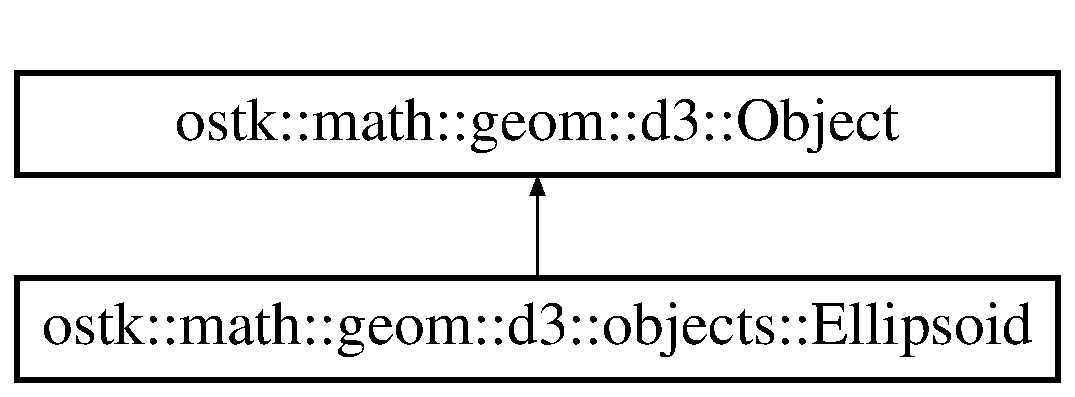
\includegraphics[height=2.000000cm]{classostk_1_1math_1_1geom_1_1d3_1_1objects_1_1_ellipsoid}
\end{center}
\end{figure}
\doxysubsection*{Public Member Functions}
\begin{DoxyCompactItemize}
\item 
\mbox{\hyperlink{classostk_1_1math_1_1geom_1_1d3_1_1objects_1_1_ellipsoid_a106c71abf9503f3d06b2613c1c7e9d65}{Ellipsoid}} (const \mbox{\hyperlink{classostk_1_1math_1_1geom_1_1d3_1_1objects_1_1_point}{Point}} \&a\+Center, const Real \&a\+First\+Principal\+Semi\+Axis, const Real \&a\+Second\+Principal\+Semi\+Axis, const Real \&a\+Third\+Principal\+Semi\+Axis, const \mbox{\hyperlink{classostk_1_1math_1_1geom_1_1d3_1_1trf_1_1rot_1_1_quaternion}{Quaternion}} \&an\+Orientation=\mbox{\hyperlink{_ellipsoid_8hpp_a5c684aeaeb24d197904b5a34839d2dd9}{D\+E\+F\+A\+U\+L\+T\+\_\+\+O\+R\+I\+E\+N\+T\+A\+T\+I\+ON}})
\begin{DoxyCompactList}\small\item\em Constructor. \end{DoxyCompactList}\item 
virtual \mbox{\hyperlink{classostk_1_1math_1_1geom_1_1d3_1_1objects_1_1_ellipsoid}{Ellipsoid}} $\ast$ \mbox{\hyperlink{classostk_1_1math_1_1geom_1_1d3_1_1objects_1_1_ellipsoid_a00899cd0b86395c4beef6947497bfe82}{clone}} () const override
\begin{DoxyCompactList}\small\item\em Clone ellipsoid. \end{DoxyCompactList}\item 
bool \mbox{\hyperlink{classostk_1_1math_1_1geom_1_1d3_1_1objects_1_1_ellipsoid_add7aa81a702b745d73f44b81359ecc4b}{operator==}} (const \mbox{\hyperlink{classostk_1_1math_1_1geom_1_1d3_1_1objects_1_1_ellipsoid}{Ellipsoid}} \&an\+Ellipsoid) const
\begin{DoxyCompactList}\small\item\em Equal to operator. \end{DoxyCompactList}\item 
bool \mbox{\hyperlink{classostk_1_1math_1_1geom_1_1d3_1_1objects_1_1_ellipsoid_aaeed509e3703368fe9f0513d5807f9cb}{operator!=}} (const \mbox{\hyperlink{classostk_1_1math_1_1geom_1_1d3_1_1objects_1_1_ellipsoid}{Ellipsoid}} \&an\+Ellipsoid) const
\begin{DoxyCompactList}\small\item\em Not equal to operator. \end{DoxyCompactList}\item 
virtual bool \mbox{\hyperlink{classostk_1_1math_1_1geom_1_1d3_1_1objects_1_1_ellipsoid_a21c465d185052a1631fe3ddcc131512d}{is\+Defined}} () const override
\begin{DoxyCompactList}\small\item\em Check if ellipsoid is defined. \end{DoxyCompactList}\item 
bool \mbox{\hyperlink{classostk_1_1math_1_1geom_1_1d3_1_1objects_1_1_ellipsoid_ac138fc763cca5a3687be35fe6cdba586}{intersects}} (const \mbox{\hyperlink{classostk_1_1math_1_1geom_1_1d3_1_1objects_1_1_point}{Point}} \&a\+Point) const
\begin{DoxyCompactList}\small\item\em Check if ellipsoid intersects point. \end{DoxyCompactList}\item 
bool \mbox{\hyperlink{classostk_1_1math_1_1geom_1_1d3_1_1objects_1_1_ellipsoid_aba612161728349d5302ce7625674893e}{intersects}} (const \mbox{\hyperlink{classostk_1_1math_1_1geom_1_1d3_1_1objects_1_1_point_set}{Point\+Set}} \&a\+Point\+Set) const
\begin{DoxyCompactList}\small\item\em Check if ellipsoid intersects point set. \end{DoxyCompactList}\item 
bool \mbox{\hyperlink{classostk_1_1math_1_1geom_1_1d3_1_1objects_1_1_ellipsoid_ade6288d324e3227eafd0126fc4680471}{intersects}} (const \mbox{\hyperlink{classostk_1_1math_1_1geom_1_1d3_1_1objects_1_1_line}{Line}} \&a\+Line) const
\begin{DoxyCompactList}\small\item\em Check if ellipsoid intersects line. \end{DoxyCompactList}\item 
bool \mbox{\hyperlink{classostk_1_1math_1_1geom_1_1d3_1_1objects_1_1_ellipsoid_aa12b5c24a22e121b18c3022ce0534a29}{intersects}} (const \mbox{\hyperlink{classostk_1_1math_1_1geom_1_1d3_1_1objects_1_1_ray}{Ray}} \&a\+Ray) const
\begin{DoxyCompactList}\small\item\em Check if ellipsoid intersects ray. \end{DoxyCompactList}\item 
bool \mbox{\hyperlink{classostk_1_1math_1_1geom_1_1d3_1_1objects_1_1_ellipsoid_ac7fc0339626b86b044d3c1a8fc174211}{intersects}} (const \mbox{\hyperlink{classostk_1_1math_1_1geom_1_1d3_1_1objects_1_1_segment}{Segment}} \&a\+Segment) const
\begin{DoxyCompactList}\small\item\em Check if ellipsoid intersects segment. \end{DoxyCompactList}\item 
bool \mbox{\hyperlink{classostk_1_1math_1_1geom_1_1d3_1_1objects_1_1_ellipsoid_a996a2dfe962cdb5dd5b16e3ee9bfdf62}{intersects}} (const \mbox{\hyperlink{classostk_1_1math_1_1geom_1_1d3_1_1objects_1_1_plane}{Plane}} \&a\+Plane) const
\begin{DoxyCompactList}\small\item\em Check if ellipsoid intersects plane. \end{DoxyCompactList}\item 
bool \mbox{\hyperlink{classostk_1_1math_1_1geom_1_1d3_1_1objects_1_1_ellipsoid_a48ab2b6828f42a314b185709126a0c43}{intersects}} (const \mbox{\hyperlink{classostk_1_1math_1_1geom_1_1d3_1_1objects_1_1_sphere}{Sphere}} \&a\+Sphere) const
\begin{DoxyCompactList}\small\item\em Check if ellipsoid intersects sphere. \end{DoxyCompactList}\item 
bool \mbox{\hyperlink{classostk_1_1math_1_1geom_1_1d3_1_1objects_1_1_ellipsoid_a2e886a6b074d7feada943ebc60f3d873}{intersects}} (const \mbox{\hyperlink{classostk_1_1math_1_1geom_1_1d3_1_1objects_1_1_ellipsoid}{Ellipsoid}} \&an\+Ellipsoid) const
\begin{DoxyCompactList}\small\item\em Check if ellipsoid intersects ellipsoid. \end{DoxyCompactList}\item 
bool \mbox{\hyperlink{classostk_1_1math_1_1geom_1_1d3_1_1objects_1_1_ellipsoid_a52ec9908e019762565ea341577b82944}{intersects}} (const \mbox{\hyperlink{classostk_1_1math_1_1geom_1_1d3_1_1objects_1_1_pyramid}{Pyramid}} \&a\+Pyramid) const
\begin{DoxyCompactList}\small\item\em Check if ellipsoid intersects pyramid. \end{DoxyCompactList}\item 
bool \mbox{\hyperlink{classostk_1_1math_1_1geom_1_1d3_1_1objects_1_1_ellipsoid_a74c6079e4c8d798892438f9560532f86}{intersects}} (const \mbox{\hyperlink{classostk_1_1math_1_1geom_1_1d3_1_1objects_1_1_cone}{Cone}} \&a\+Cone) const
\begin{DoxyCompactList}\small\item\em Check if ellipsoid intersects cone. \end{DoxyCompactList}\item 
bool \mbox{\hyperlink{classostk_1_1math_1_1geom_1_1d3_1_1objects_1_1_ellipsoid_a65985adadbc7de1e595c7ed326725f92}{contains}} (const \mbox{\hyperlink{classostk_1_1math_1_1geom_1_1d3_1_1objects_1_1_point}{Point}} \&a\+Point) const
\begin{DoxyCompactList}\small\item\em Check if ellipsoid contains point. \end{DoxyCompactList}\item 
bool \mbox{\hyperlink{classostk_1_1math_1_1geom_1_1d3_1_1objects_1_1_ellipsoid_a9e0b0c5c2db95f53da783ccfea36de17}{contains}} (const \mbox{\hyperlink{classostk_1_1math_1_1geom_1_1d3_1_1objects_1_1_point_set}{Point\+Set}} \&a\+Point\+Set) const
\begin{DoxyCompactList}\small\item\em Check if ellipsoid contains point set. \end{DoxyCompactList}\item 
bool \mbox{\hyperlink{classostk_1_1math_1_1geom_1_1d3_1_1objects_1_1_ellipsoid_afcb41440d899c60766cdc7e9c838c55d}{contains}} (const \mbox{\hyperlink{classostk_1_1math_1_1geom_1_1d3_1_1objects_1_1_segment}{Segment}} \&a\+Segment) const
\begin{DoxyCompactList}\small\item\em Check if ellipsoid contains segment. \end{DoxyCompactList}\item 
\mbox{\hyperlink{classostk_1_1math_1_1geom_1_1d3_1_1objects_1_1_point}{Point}} \mbox{\hyperlink{classostk_1_1math_1_1geom_1_1d3_1_1objects_1_1_ellipsoid_a0b1f86eb5b3cb20a8306a951a6006d4e}{get\+Center}} () const
\begin{DoxyCompactList}\small\item\em Get ellipsoid center. \end{DoxyCompactList}\item 
Real \mbox{\hyperlink{classostk_1_1math_1_1geom_1_1d3_1_1objects_1_1_ellipsoid_a0d922209dffb806def71604d7dde2ba7}{get\+First\+Principal\+Semi\+Axis}} () const
\begin{DoxyCompactList}\small\item\em Get ellipsoid first principal semi-\/axis. \end{DoxyCompactList}\item 
Real \mbox{\hyperlink{classostk_1_1math_1_1geom_1_1d3_1_1objects_1_1_ellipsoid_a628df5e41c5b24722c74b54f604788da}{get\+Second\+Principal\+Semi\+Axis}} () const
\begin{DoxyCompactList}\small\item\em Get ellipsoid second principal semi-\/axis. \end{DoxyCompactList}\item 
Real \mbox{\hyperlink{classostk_1_1math_1_1geom_1_1d3_1_1objects_1_1_ellipsoid_aa0439388600dc3b6dc93d26402ae2d6d}{get\+Third\+Principal\+Semi\+Axis}} () const
\begin{DoxyCompactList}\small\item\em Get ellipsoid third principal semi-\/axis. \end{DoxyCompactList}\item 
Vector3d \mbox{\hyperlink{classostk_1_1math_1_1geom_1_1d3_1_1objects_1_1_ellipsoid_a29d6b71247c279c5940c1ede221a5aac}{get\+First\+Axis}} () const
\begin{DoxyCompactList}\small\item\em Get ellipsoid first axis. \end{DoxyCompactList}\item 
Vector3d \mbox{\hyperlink{classostk_1_1math_1_1geom_1_1d3_1_1objects_1_1_ellipsoid_a9a694ec8f31e617d4101bd31fa1519a0}{get\+Second\+Axis}} () const
\begin{DoxyCompactList}\small\item\em Get ellipsoid second axis. \end{DoxyCompactList}\item 
Vector3d \mbox{\hyperlink{classostk_1_1math_1_1geom_1_1d3_1_1objects_1_1_ellipsoid_a2e12dada2181d15c8cf4cef2abf3d2ea}{get\+Third\+Axis}} () const
\begin{DoxyCompactList}\small\item\em Get ellipsoid third axis. \end{DoxyCompactList}\item 
\mbox{\hyperlink{classostk_1_1math_1_1geom_1_1d3_1_1trf_1_1rot_1_1_quaternion}{Quaternion}} \mbox{\hyperlink{classostk_1_1math_1_1geom_1_1d3_1_1objects_1_1_ellipsoid_a3e273d94d0ff1d40e3588d5ee2366ec9}{get\+Orientation}} () const
\begin{DoxyCompactList}\small\item\em Get ellipsoid orientation. \end{DoxyCompactList}\item 
Matrix3d \mbox{\hyperlink{classostk_1_1math_1_1geom_1_1d3_1_1objects_1_1_ellipsoid_aea24d2d268d701c31a18f2ddac2cd394}{get\+Matrix}} () const
\begin{DoxyCompactList}\small\item\em Get ellipsoid matrix. \end{DoxyCompactList}\item 
\mbox{\hyperlink{classostk_1_1math_1_1geom_1_1d3_1_1_intersection}{Intersection}} \mbox{\hyperlink{classostk_1_1math_1_1geom_1_1d3_1_1objects_1_1_ellipsoid_a18e2c5add63d0f1ed857a3cda95ceb10}{intersection\+With}} (const \mbox{\hyperlink{classostk_1_1math_1_1geom_1_1d3_1_1objects_1_1_line}{Line}} \&a\+Line) const
\begin{DoxyCompactList}\small\item\em Compute intersection of ellipsoid with line. \end{DoxyCompactList}\item 
\mbox{\hyperlink{classostk_1_1math_1_1geom_1_1d3_1_1_intersection}{Intersection}} \mbox{\hyperlink{classostk_1_1math_1_1geom_1_1d3_1_1objects_1_1_ellipsoid_ae062bed9d63b86032ba55db7e3d130be}{intersection\+With}} (const \mbox{\hyperlink{classostk_1_1math_1_1geom_1_1d3_1_1objects_1_1_ray}{Ray}} \&a\+Ray, const bool only\+In\+Sight=false) const
\begin{DoxyCompactList}\small\item\em Compute intersection of ellipsoid with ray. \end{DoxyCompactList}\item 
\mbox{\hyperlink{classostk_1_1math_1_1geom_1_1d3_1_1_intersection}{Intersection}} \mbox{\hyperlink{classostk_1_1math_1_1geom_1_1d3_1_1objects_1_1_ellipsoid_a28e2a2bfdbbcc0e4141c3cb7434a5c5a}{intersection\+With}} (const \mbox{\hyperlink{classostk_1_1math_1_1geom_1_1d3_1_1objects_1_1_segment}{Segment}} \&a\+Segment) const
\begin{DoxyCompactList}\small\item\em Compute intersection of ellipsoid with segment. \end{DoxyCompactList}\item 
\mbox{\hyperlink{classostk_1_1math_1_1geom_1_1d3_1_1_intersection}{Intersection}} \mbox{\hyperlink{classostk_1_1math_1_1geom_1_1d3_1_1objects_1_1_ellipsoid_aad7841b85e90ebe3ca429772c124033e}{intersection\+With}} (const \mbox{\hyperlink{classostk_1_1math_1_1geom_1_1d3_1_1objects_1_1_pyramid}{Pyramid}} \&a\+Pyramid, const bool only\+In\+Sight=false) const
\begin{DoxyCompactList}\small\item\em Compute intersection of ellipsoid with pyramid. \end{DoxyCompactList}\item 
\mbox{\hyperlink{classostk_1_1math_1_1geom_1_1d3_1_1_intersection}{Intersection}} \mbox{\hyperlink{classostk_1_1math_1_1geom_1_1d3_1_1objects_1_1_ellipsoid_adb4af12ad6a14e483971926822da732c}{intersection\+With}} (const \mbox{\hyperlink{classostk_1_1math_1_1geom_1_1d3_1_1objects_1_1_cone}{Cone}} \&a\+Cone, const bool only\+In\+Sight=false) const
\begin{DoxyCompactList}\small\item\em Compute intersection of ellipsoid with cone. \end{DoxyCompactList}\item 
virtual void \mbox{\hyperlink{classostk_1_1math_1_1geom_1_1d3_1_1objects_1_1_ellipsoid_a650fa20181d61ea455b98fc3330baf6e}{print}} (std\+::ostream \&an\+Output\+Stream, bool display\+Decorators=true) const override
\begin{DoxyCompactList}\small\item\em Print ellipsoid. \end{DoxyCompactList}\item 
virtual void \mbox{\hyperlink{classostk_1_1math_1_1geom_1_1d3_1_1objects_1_1_ellipsoid_aa7c60b942f6b1fa3a513bc3b549ab9e6}{apply\+Transformation}} (const \mbox{\hyperlink{classostk_1_1math_1_1geom_1_1d3_1_1_transformation}{Transformation}} \&a\+Transformation) override
\begin{DoxyCompactList}\small\item\em Apply transformation to ellipsoid. \end{DoxyCompactList}\end{DoxyCompactItemize}
\doxysubsection*{Static Public Member Functions}
\begin{DoxyCompactItemize}
\item 
static \mbox{\hyperlink{classostk_1_1math_1_1geom_1_1d3_1_1objects_1_1_ellipsoid}{Ellipsoid}} \mbox{\hyperlink{classostk_1_1math_1_1geom_1_1d3_1_1objects_1_1_ellipsoid_a607399f86f75b9f2c97f05802b0974b2}{Undefined}} ()
\begin{DoxyCompactList}\small\item\em Constructs an undefined ellipsoid. \end{DoxyCompactList}\end{DoxyCompactItemize}


\doxysubsection{Detailed Description}
\mbox{\hyperlink{classostk_1_1math_1_1geom_1_1d3_1_1objects_1_1_ellipsoid}{Ellipsoid}}. 

\href{https://en.wikipedia.org/wiki/Ellipsoid}{\texttt{ https\+://en.\+wikipedia.\+org/wiki/\+Ellipsoid}} 

\doxysubsection{Constructor \& Destructor Documentation}
\mbox{\Hypertarget{classostk_1_1math_1_1geom_1_1d3_1_1objects_1_1_ellipsoid_a106c71abf9503f3d06b2613c1c7e9d65}\label{classostk_1_1math_1_1geom_1_1d3_1_1objects_1_1_ellipsoid_a106c71abf9503f3d06b2613c1c7e9d65}} 
\index{ostk::math::geom::d3::objects::Ellipsoid@{ostk::math::geom::d3::objects::Ellipsoid}!Ellipsoid@{Ellipsoid}}
\index{Ellipsoid@{Ellipsoid}!ostk::math::geom::d3::objects::Ellipsoid@{ostk::math::geom::d3::objects::Ellipsoid}}
\doxysubsubsection{\texorpdfstring{Ellipsoid()}{Ellipsoid()}}
{\footnotesize\ttfamily ostk\+::math\+::geom\+::d3\+::objects\+::\+Ellipsoid\+::\+Ellipsoid (\begin{DoxyParamCaption}\item[{const \mbox{\hyperlink{classostk_1_1math_1_1geom_1_1d3_1_1objects_1_1_point}{Point}} \&}]{a\+Center,  }\item[{const Real \&}]{a\+First\+Principal\+Semi\+Axis,  }\item[{const Real \&}]{a\+Second\+Principal\+Semi\+Axis,  }\item[{const Real \&}]{a\+Third\+Principal\+Semi\+Axis,  }\item[{const \mbox{\hyperlink{classostk_1_1math_1_1geom_1_1d3_1_1trf_1_1rot_1_1_quaternion}{Quaternion}} \&}]{an\+Orientation = {\ttfamily \mbox{\hyperlink{_ellipsoid_8hpp_a5c684aeaeb24d197904b5a34839d2dd9}{D\+E\+F\+A\+U\+L\+T\+\_\+\+O\+R\+I\+E\+N\+T\+A\+T\+I\+ON}}} }\end{DoxyParamCaption})}



Constructor. 


\begin{DoxyCode}{0}
\DoxyCodeLine{\mbox{\hyperlink{classostk_1_1math_1_1geom_1_1d3_1_1objects_1_1_ellipsoid_a106c71abf9503f3d06b2613c1c7e9d65}{Ellipsoid}} ellipsoid(\{ 0.0, 0.0, 0.0 \}, 1.0, 2.0, 3.0) ;}
\end{DoxyCode}



\begin{DoxyParams}[1]{Parameters}
\mbox{\texttt{ in}}  & {\em a\+Center} & An ellipsoid center \\
\hline
\mbox{\texttt{ in}}  & {\em a\+First\+Principal\+Semi\+Axis} & An ellipsoid first principal semi-\/axis \\
\hline
\mbox{\texttt{ in}}  & {\em a\+Second\+Principal\+Semi\+Axis} & An ellipsoid second principal semi-\/axis \\
\hline
\mbox{\texttt{ in}}  & {\em a\+Third\+Principal\+Semi\+Axis} & An ellipsoid third principal semi-\/axis \\
\hline
\mbox{\texttt{ in}}  & {\em (optional)} & an\+Orientation An ellipsoid orientation \\
\hline
\end{DoxyParams}


\doxysubsection{Member Function Documentation}
\mbox{\Hypertarget{classostk_1_1math_1_1geom_1_1d3_1_1objects_1_1_ellipsoid_aa7c60b942f6b1fa3a513bc3b549ab9e6}\label{classostk_1_1math_1_1geom_1_1d3_1_1objects_1_1_ellipsoid_aa7c60b942f6b1fa3a513bc3b549ab9e6}} 
\index{ostk::math::geom::d3::objects::Ellipsoid@{ostk::math::geom::d3::objects::Ellipsoid}!applyTransformation@{applyTransformation}}
\index{applyTransformation@{applyTransformation}!ostk::math::geom::d3::objects::Ellipsoid@{ostk::math::geom::d3::objects::Ellipsoid}}
\doxysubsubsection{\texorpdfstring{applyTransformation()}{applyTransformation()}}
{\footnotesize\ttfamily void ostk\+::math\+::geom\+::d3\+::objects\+::\+Ellipsoid\+::apply\+Transformation (\begin{DoxyParamCaption}\item[{const \mbox{\hyperlink{classostk_1_1math_1_1geom_1_1d3_1_1_transformation}{Transformation}} \&}]{a\+Transformation }\end{DoxyParamCaption})\hspace{0.3cm}{\ttfamily [override]}, {\ttfamily [virtual]}}



Apply transformation to ellipsoid. 


\begin{DoxyParams}[1]{Parameters}
\mbox{\texttt{ in}}  & {\em a\+Transformation} & A transformation \\
\hline
\end{DoxyParams}


Implements \mbox{\hyperlink{classostk_1_1math_1_1geom_1_1d3_1_1_object_ae9194dd6d2bb4df09292ffc84dccdb1d}{ostk\+::math\+::geom\+::d3\+::\+Object}}.

\mbox{\Hypertarget{classostk_1_1math_1_1geom_1_1d3_1_1objects_1_1_ellipsoid_a00899cd0b86395c4beef6947497bfe82}\label{classostk_1_1math_1_1geom_1_1d3_1_1objects_1_1_ellipsoid_a00899cd0b86395c4beef6947497bfe82}} 
\index{ostk::math::geom::d3::objects::Ellipsoid@{ostk::math::geom::d3::objects::Ellipsoid}!clone@{clone}}
\index{clone@{clone}!ostk::math::geom::d3::objects::Ellipsoid@{ostk::math::geom::d3::objects::Ellipsoid}}
\doxysubsubsection{\texorpdfstring{clone()}{clone()}}
{\footnotesize\ttfamily \mbox{\hyperlink{classostk_1_1math_1_1geom_1_1d3_1_1objects_1_1_ellipsoid}{Ellipsoid}} $\ast$ ostk\+::math\+::geom\+::d3\+::objects\+::\+Ellipsoid\+::clone (\begin{DoxyParamCaption}{ }\end{DoxyParamCaption}) const\hspace{0.3cm}{\ttfamily [override]}, {\ttfamily [virtual]}}



Clone ellipsoid. 

\begin{DoxyReturn}{Returns}
Pointer to cloned ellipsoid 
\end{DoxyReturn}


Implements \mbox{\hyperlink{classostk_1_1math_1_1geom_1_1d3_1_1_object_a676013f9555f6492687f9809b2db887b}{ostk\+::math\+::geom\+::d3\+::\+Object}}.

\mbox{\Hypertarget{classostk_1_1math_1_1geom_1_1d3_1_1objects_1_1_ellipsoid_a65985adadbc7de1e595c7ed326725f92}\label{classostk_1_1math_1_1geom_1_1d3_1_1objects_1_1_ellipsoid_a65985adadbc7de1e595c7ed326725f92}} 
\index{ostk::math::geom::d3::objects::Ellipsoid@{ostk::math::geom::d3::objects::Ellipsoid}!contains@{contains}}
\index{contains@{contains}!ostk::math::geom::d3::objects::Ellipsoid@{ostk::math::geom::d3::objects::Ellipsoid}}
\doxysubsubsection{\texorpdfstring{contains()}{contains()}\hspace{0.1cm}{\footnotesize\ttfamily [1/3]}}
{\footnotesize\ttfamily bool ostk\+::math\+::geom\+::d3\+::objects\+::\+Ellipsoid\+::contains (\begin{DoxyParamCaption}\item[{const \mbox{\hyperlink{classostk_1_1math_1_1geom_1_1d3_1_1objects_1_1_point}{Point}} \&}]{a\+Point }\end{DoxyParamCaption}) const}



Check if ellipsoid contains point. 


\begin{DoxyCode}{0}
\DoxyCodeLine{\mbox{\hyperlink{classostk_1_1math_1_1geom_1_1d3_1_1objects_1_1_ellipsoid_a106c71abf9503f3d06b2613c1c7e9d65}{Ellipsoid}} ellipsoid = ... ;}
\DoxyCodeLine{Point point = ... ;}
\DoxyCodeLine{ellipsoid.contains(point) ;}
\end{DoxyCode}



\begin{DoxyParams}[1]{Parameters}
\mbox{\texttt{ in}}  & {\em a\+Point} & A point \\
\hline
\end{DoxyParams}
\begin{DoxyReturn}{Returns}
True if ellipsoid contains point 
\end{DoxyReturn}
\mbox{\Hypertarget{classostk_1_1math_1_1geom_1_1d3_1_1objects_1_1_ellipsoid_a9e0b0c5c2db95f53da783ccfea36de17}\label{classostk_1_1math_1_1geom_1_1d3_1_1objects_1_1_ellipsoid_a9e0b0c5c2db95f53da783ccfea36de17}} 
\index{ostk::math::geom::d3::objects::Ellipsoid@{ostk::math::geom::d3::objects::Ellipsoid}!contains@{contains}}
\index{contains@{contains}!ostk::math::geom::d3::objects::Ellipsoid@{ostk::math::geom::d3::objects::Ellipsoid}}
\doxysubsubsection{\texorpdfstring{contains()}{contains()}\hspace{0.1cm}{\footnotesize\ttfamily [2/3]}}
{\footnotesize\ttfamily bool ostk\+::math\+::geom\+::d3\+::objects\+::\+Ellipsoid\+::contains (\begin{DoxyParamCaption}\item[{const \mbox{\hyperlink{classostk_1_1math_1_1geom_1_1d3_1_1objects_1_1_point_set}{Point\+Set}} \&}]{a\+Point\+Set }\end{DoxyParamCaption}) const}



Check if ellipsoid contains point set. 


\begin{DoxyCode}{0}
\DoxyCodeLine{\mbox{\hyperlink{classostk_1_1math_1_1geom_1_1d3_1_1objects_1_1_ellipsoid_a106c71abf9503f3d06b2613c1c7e9d65}{Ellipsoid}} ellipsoid = ... ;}
\DoxyCodeLine{PointSet pointSet = ... ;}
\DoxyCodeLine{ellipsoid.contains(pointSet) ;}
\end{DoxyCode}



\begin{DoxyParams}[1]{Parameters}
\mbox{\texttt{ in}}  & {\em a\+Point\+Set} & A point set \\
\hline
\end{DoxyParams}
\begin{DoxyReturn}{Returns}
True if ellipsoid contains point set 
\end{DoxyReturn}
\mbox{\Hypertarget{classostk_1_1math_1_1geom_1_1d3_1_1objects_1_1_ellipsoid_afcb41440d899c60766cdc7e9c838c55d}\label{classostk_1_1math_1_1geom_1_1d3_1_1objects_1_1_ellipsoid_afcb41440d899c60766cdc7e9c838c55d}} 
\index{ostk::math::geom::d3::objects::Ellipsoid@{ostk::math::geom::d3::objects::Ellipsoid}!contains@{contains}}
\index{contains@{contains}!ostk::math::geom::d3::objects::Ellipsoid@{ostk::math::geom::d3::objects::Ellipsoid}}
\doxysubsubsection{\texorpdfstring{contains()}{contains()}\hspace{0.1cm}{\footnotesize\ttfamily [3/3]}}
{\footnotesize\ttfamily bool ostk\+::math\+::geom\+::d3\+::objects\+::\+Ellipsoid\+::contains (\begin{DoxyParamCaption}\item[{const \mbox{\hyperlink{classostk_1_1math_1_1geom_1_1d3_1_1objects_1_1_segment}{Segment}} \&}]{a\+Segment }\end{DoxyParamCaption}) const}



Check if ellipsoid contains segment. 


\begin{DoxyCode}{0}
\DoxyCodeLine{\mbox{\hyperlink{classostk_1_1math_1_1geom_1_1d3_1_1objects_1_1_ellipsoid_a106c71abf9503f3d06b2613c1c7e9d65}{Ellipsoid}} ellipsoid = ... ;}
\DoxyCodeLine{Segment segment = ... ;}
\DoxyCodeLine{ellipsoid.contains(segment) ;}
\end{DoxyCode}



\begin{DoxyParams}[1]{Parameters}
\mbox{\texttt{ in}}  & {\em a\+Segment} & A segment \\
\hline
\end{DoxyParams}
\begin{DoxyReturn}{Returns}
True if ellipsoid contains segment 
\end{DoxyReturn}
\mbox{\Hypertarget{classostk_1_1math_1_1geom_1_1d3_1_1objects_1_1_ellipsoid_a0b1f86eb5b3cb20a8306a951a6006d4e}\label{classostk_1_1math_1_1geom_1_1d3_1_1objects_1_1_ellipsoid_a0b1f86eb5b3cb20a8306a951a6006d4e}} 
\index{ostk::math::geom::d3::objects::Ellipsoid@{ostk::math::geom::d3::objects::Ellipsoid}!getCenter@{getCenter}}
\index{getCenter@{getCenter}!ostk::math::geom::d3::objects::Ellipsoid@{ostk::math::geom::d3::objects::Ellipsoid}}
\doxysubsubsection{\texorpdfstring{getCenter()}{getCenter()}}
{\footnotesize\ttfamily \mbox{\hyperlink{classostk_1_1math_1_1geom_1_1d3_1_1objects_1_1_point}{Point}} ostk\+::math\+::geom\+::d3\+::objects\+::\+Ellipsoid\+::get\+Center (\begin{DoxyParamCaption}{ }\end{DoxyParamCaption}) const}



Get ellipsoid center. 


\begin{DoxyCode}{0}
\DoxyCodeLine{\mbox{\hyperlink{classostk_1_1math_1_1geom_1_1d3_1_1objects_1_1_ellipsoid_a106c71abf9503f3d06b2613c1c7e9d65}{Ellipsoid}}(\mbox{\hyperlink{classostk_1_1math_1_1geom_1_1d3_1_1objects_1_1_point_a079c199f08b015d456d02728a71b534c}{Point::Origin}}(), 1.0, 2.0, 3.0).getCenter() ; \textcolor{comment}{// [0.0, 0.0, 0.0]}}
\end{DoxyCode}


\begin{DoxyReturn}{Returns}
\mbox{\hyperlink{classostk_1_1math_1_1geom_1_1d3_1_1objects_1_1_ellipsoid}{Ellipsoid}} center 
\end{DoxyReturn}
\mbox{\Hypertarget{classostk_1_1math_1_1geom_1_1d3_1_1objects_1_1_ellipsoid_a29d6b71247c279c5940c1ede221a5aac}\label{classostk_1_1math_1_1geom_1_1d3_1_1objects_1_1_ellipsoid_a29d6b71247c279c5940c1ede221a5aac}} 
\index{ostk::math::geom::d3::objects::Ellipsoid@{ostk::math::geom::d3::objects::Ellipsoid}!getFirstAxis@{getFirstAxis}}
\index{getFirstAxis@{getFirstAxis}!ostk::math::geom::d3::objects::Ellipsoid@{ostk::math::geom::d3::objects::Ellipsoid}}
\doxysubsubsection{\texorpdfstring{getFirstAxis()}{getFirstAxis()}}
{\footnotesize\ttfamily Vector3d ostk\+::math\+::geom\+::d3\+::objects\+::\+Ellipsoid\+::get\+First\+Axis (\begin{DoxyParamCaption}{ }\end{DoxyParamCaption}) const}



Get ellipsoid first axis. 

\begin{DoxyReturn}{Returns}
\mbox{\hyperlink{classostk_1_1math_1_1geom_1_1d3_1_1objects_1_1_ellipsoid}{Ellipsoid}} first axis 
\end{DoxyReturn}
\mbox{\Hypertarget{classostk_1_1math_1_1geom_1_1d3_1_1objects_1_1_ellipsoid_a0d922209dffb806def71604d7dde2ba7}\label{classostk_1_1math_1_1geom_1_1d3_1_1objects_1_1_ellipsoid_a0d922209dffb806def71604d7dde2ba7}} 
\index{ostk::math::geom::d3::objects::Ellipsoid@{ostk::math::geom::d3::objects::Ellipsoid}!getFirstPrincipalSemiAxis@{getFirstPrincipalSemiAxis}}
\index{getFirstPrincipalSemiAxis@{getFirstPrincipalSemiAxis}!ostk::math::geom::d3::objects::Ellipsoid@{ostk::math::geom::d3::objects::Ellipsoid}}
\doxysubsubsection{\texorpdfstring{getFirstPrincipalSemiAxis()}{getFirstPrincipalSemiAxis()}}
{\footnotesize\ttfamily Real ostk\+::math\+::geom\+::d3\+::objects\+::\+Ellipsoid\+::get\+First\+Principal\+Semi\+Axis (\begin{DoxyParamCaption}{ }\end{DoxyParamCaption}) const}



Get ellipsoid first principal semi-\/axis. 


\begin{DoxyCode}{0}
\DoxyCodeLine{\mbox{\hyperlink{classostk_1_1math_1_1geom_1_1d3_1_1objects_1_1_ellipsoid_a106c71abf9503f3d06b2613c1c7e9d65}{Ellipsoid}}(\mbox{\hyperlink{classostk_1_1math_1_1geom_1_1d3_1_1objects_1_1_point_a079c199f08b015d456d02728a71b534c}{Point::Origin}}(), 1.0, 2.0, 3.0).getFirstPrincipalSemiAxis() ; \textcolor{comment}{// 1.0}}
\end{DoxyCode}


\begin{DoxyReturn}{Returns}
\mbox{\hyperlink{classostk_1_1math_1_1geom_1_1d3_1_1objects_1_1_ellipsoid}{Ellipsoid}} first principal semi-\/axis 
\end{DoxyReturn}
\mbox{\Hypertarget{classostk_1_1math_1_1geom_1_1d3_1_1objects_1_1_ellipsoid_aea24d2d268d701c31a18f2ddac2cd394}\label{classostk_1_1math_1_1geom_1_1d3_1_1objects_1_1_ellipsoid_aea24d2d268d701c31a18f2ddac2cd394}} 
\index{ostk::math::geom::d3::objects::Ellipsoid@{ostk::math::geom::d3::objects::Ellipsoid}!getMatrix@{getMatrix}}
\index{getMatrix@{getMatrix}!ostk::math::geom::d3::objects::Ellipsoid@{ostk::math::geom::d3::objects::Ellipsoid}}
\doxysubsubsection{\texorpdfstring{getMatrix()}{getMatrix()}}
{\footnotesize\ttfamily Matrix3d ostk\+::math\+::geom\+::d3\+::objects\+::\+Ellipsoid\+::get\+Matrix (\begin{DoxyParamCaption}{ }\end{DoxyParamCaption}) const}



Get ellipsoid matrix. 


\begin{DoxyCode}{0}
\DoxyCodeLine{\mbox{\hyperlink{classostk_1_1math_1_1geom_1_1d3_1_1objects_1_1_ellipsoid_a106c71abf9503f3d06b2613c1c7e9d65}{Ellipsoid}}(\mbox{\hyperlink{classostk_1_1math_1_1geom_1_1d3_1_1objects_1_1_point_a079c199f08b015d456d02728a71b534c}{Point::Origin}}(), 1.0, 2.0, 3.0, \mbox{\hyperlink{classostk_1_1math_1_1geom_1_1d3_1_1trf_1_1rot_1_1_quaternion_ac57ea57a4033622ed1389101b2e58c76}{Quaternion::XYZS}}(0.0, 0.0, 0.0, 1.0)).getMatrix()}
\DoxyCodeLine{;}
\end{DoxyCode}


\begin{DoxyReturn}{Returns}
\mbox{\hyperlink{classostk_1_1math_1_1geom_1_1d3_1_1objects_1_1_ellipsoid}{Ellipsoid}} matrix 
\end{DoxyReturn}
\mbox{\Hypertarget{classostk_1_1math_1_1geom_1_1d3_1_1objects_1_1_ellipsoid_a3e273d94d0ff1d40e3588d5ee2366ec9}\label{classostk_1_1math_1_1geom_1_1d3_1_1objects_1_1_ellipsoid_a3e273d94d0ff1d40e3588d5ee2366ec9}} 
\index{ostk::math::geom::d3::objects::Ellipsoid@{ostk::math::geom::d3::objects::Ellipsoid}!getOrientation@{getOrientation}}
\index{getOrientation@{getOrientation}!ostk::math::geom::d3::objects::Ellipsoid@{ostk::math::geom::d3::objects::Ellipsoid}}
\doxysubsubsection{\texorpdfstring{getOrientation()}{getOrientation()}}
{\footnotesize\ttfamily \mbox{\hyperlink{classostk_1_1math_1_1geom_1_1d3_1_1trf_1_1rot_1_1_quaternion}{Quaternion}} ostk\+::math\+::geom\+::d3\+::objects\+::\+Ellipsoid\+::get\+Orientation (\begin{DoxyParamCaption}{ }\end{DoxyParamCaption}) const}



Get ellipsoid orientation. 


\begin{DoxyCode}{0}
\DoxyCodeLine{\mbox{\hyperlink{classostk_1_1math_1_1geom_1_1d3_1_1objects_1_1_ellipsoid_a106c71abf9503f3d06b2613c1c7e9d65}{Ellipsoid}}(\mbox{\hyperlink{classostk_1_1math_1_1geom_1_1d3_1_1objects_1_1_point_a079c199f08b015d456d02728a71b534c}{Point::Origin}}(), 1.0, 2.0, 3.0, \mbox{\hyperlink{classostk_1_1math_1_1geom_1_1d3_1_1trf_1_1rot_1_1_quaternion_ac57ea57a4033622ed1389101b2e58c76}{Quaternion::XYZS}}(0.0, 0.0,}
\DoxyCodeLine{0.0, 1.0)).getOrientation() ; \textcolor{comment}{// Quaternion::XYZS(0.0, 0.0, 0.0, 1.0)}}
\end{DoxyCode}


\begin{DoxyReturn}{Returns}
\mbox{\hyperlink{classostk_1_1math_1_1geom_1_1d3_1_1objects_1_1_ellipsoid}{Ellipsoid}} orientation 
\end{DoxyReturn}
\mbox{\Hypertarget{classostk_1_1math_1_1geom_1_1d3_1_1objects_1_1_ellipsoid_a9a694ec8f31e617d4101bd31fa1519a0}\label{classostk_1_1math_1_1geom_1_1d3_1_1objects_1_1_ellipsoid_a9a694ec8f31e617d4101bd31fa1519a0}} 
\index{ostk::math::geom::d3::objects::Ellipsoid@{ostk::math::geom::d3::objects::Ellipsoid}!getSecondAxis@{getSecondAxis}}
\index{getSecondAxis@{getSecondAxis}!ostk::math::geom::d3::objects::Ellipsoid@{ostk::math::geom::d3::objects::Ellipsoid}}
\doxysubsubsection{\texorpdfstring{getSecondAxis()}{getSecondAxis()}}
{\footnotesize\ttfamily Vector3d ostk\+::math\+::geom\+::d3\+::objects\+::\+Ellipsoid\+::get\+Second\+Axis (\begin{DoxyParamCaption}{ }\end{DoxyParamCaption}) const}



Get ellipsoid second axis. 

\begin{DoxyReturn}{Returns}
\mbox{\hyperlink{classostk_1_1math_1_1geom_1_1d3_1_1objects_1_1_ellipsoid}{Ellipsoid}} second axis 
\end{DoxyReturn}
\mbox{\Hypertarget{classostk_1_1math_1_1geom_1_1d3_1_1objects_1_1_ellipsoid_a628df5e41c5b24722c74b54f604788da}\label{classostk_1_1math_1_1geom_1_1d3_1_1objects_1_1_ellipsoid_a628df5e41c5b24722c74b54f604788da}} 
\index{ostk::math::geom::d3::objects::Ellipsoid@{ostk::math::geom::d3::objects::Ellipsoid}!getSecondPrincipalSemiAxis@{getSecondPrincipalSemiAxis}}
\index{getSecondPrincipalSemiAxis@{getSecondPrincipalSemiAxis}!ostk::math::geom::d3::objects::Ellipsoid@{ostk::math::geom::d3::objects::Ellipsoid}}
\doxysubsubsection{\texorpdfstring{getSecondPrincipalSemiAxis()}{getSecondPrincipalSemiAxis()}}
{\footnotesize\ttfamily Real ostk\+::math\+::geom\+::d3\+::objects\+::\+Ellipsoid\+::get\+Second\+Principal\+Semi\+Axis (\begin{DoxyParamCaption}{ }\end{DoxyParamCaption}) const}



Get ellipsoid second principal semi-\/axis. 


\begin{DoxyCode}{0}
\DoxyCodeLine{\mbox{\hyperlink{classostk_1_1math_1_1geom_1_1d3_1_1objects_1_1_ellipsoid_a106c71abf9503f3d06b2613c1c7e9d65}{Ellipsoid}}(\mbox{\hyperlink{classostk_1_1math_1_1geom_1_1d3_1_1objects_1_1_point_a079c199f08b015d456d02728a71b534c}{Point::Origin}}(), 1.0, 2.0, 3.0).getSecondPrincipalSemiAxis() ; \textcolor{comment}{// 2.0}}
\end{DoxyCode}


\begin{DoxyReturn}{Returns}
\mbox{\hyperlink{classostk_1_1math_1_1geom_1_1d3_1_1objects_1_1_ellipsoid}{Ellipsoid}} second principal semi-\/axis 
\end{DoxyReturn}
\mbox{\Hypertarget{classostk_1_1math_1_1geom_1_1d3_1_1objects_1_1_ellipsoid_a2e12dada2181d15c8cf4cef2abf3d2ea}\label{classostk_1_1math_1_1geom_1_1d3_1_1objects_1_1_ellipsoid_a2e12dada2181d15c8cf4cef2abf3d2ea}} 
\index{ostk::math::geom::d3::objects::Ellipsoid@{ostk::math::geom::d3::objects::Ellipsoid}!getThirdAxis@{getThirdAxis}}
\index{getThirdAxis@{getThirdAxis}!ostk::math::geom::d3::objects::Ellipsoid@{ostk::math::geom::d3::objects::Ellipsoid}}
\doxysubsubsection{\texorpdfstring{getThirdAxis()}{getThirdAxis()}}
{\footnotesize\ttfamily Vector3d ostk\+::math\+::geom\+::d3\+::objects\+::\+Ellipsoid\+::get\+Third\+Axis (\begin{DoxyParamCaption}{ }\end{DoxyParamCaption}) const}



Get ellipsoid third axis. 

\begin{DoxyReturn}{Returns}
\mbox{\hyperlink{classostk_1_1math_1_1geom_1_1d3_1_1objects_1_1_ellipsoid}{Ellipsoid}} third axis 
\end{DoxyReturn}
\mbox{\Hypertarget{classostk_1_1math_1_1geom_1_1d3_1_1objects_1_1_ellipsoid_aa0439388600dc3b6dc93d26402ae2d6d}\label{classostk_1_1math_1_1geom_1_1d3_1_1objects_1_1_ellipsoid_aa0439388600dc3b6dc93d26402ae2d6d}} 
\index{ostk::math::geom::d3::objects::Ellipsoid@{ostk::math::geom::d3::objects::Ellipsoid}!getThirdPrincipalSemiAxis@{getThirdPrincipalSemiAxis}}
\index{getThirdPrincipalSemiAxis@{getThirdPrincipalSemiAxis}!ostk::math::geom::d3::objects::Ellipsoid@{ostk::math::geom::d3::objects::Ellipsoid}}
\doxysubsubsection{\texorpdfstring{getThirdPrincipalSemiAxis()}{getThirdPrincipalSemiAxis()}}
{\footnotesize\ttfamily Real ostk\+::math\+::geom\+::d3\+::objects\+::\+Ellipsoid\+::get\+Third\+Principal\+Semi\+Axis (\begin{DoxyParamCaption}{ }\end{DoxyParamCaption}) const}



Get ellipsoid third principal semi-\/axis. 


\begin{DoxyCode}{0}
\DoxyCodeLine{\mbox{\hyperlink{classostk_1_1math_1_1geom_1_1d3_1_1objects_1_1_ellipsoid_a106c71abf9503f3d06b2613c1c7e9d65}{Ellipsoid}}(\mbox{\hyperlink{classostk_1_1math_1_1geom_1_1d3_1_1objects_1_1_point_a079c199f08b015d456d02728a71b534c}{Point::Origin}}(), 1.0, 2.0, 3.0).getThirdPrincipalSemiAxis() ; \textcolor{comment}{// 3.0}}
\end{DoxyCode}


\begin{DoxyReturn}{Returns}
\mbox{\hyperlink{classostk_1_1math_1_1geom_1_1d3_1_1objects_1_1_ellipsoid}{Ellipsoid}} third principal semi-\/axis 
\end{DoxyReturn}
\mbox{\Hypertarget{classostk_1_1math_1_1geom_1_1d3_1_1objects_1_1_ellipsoid_adb4af12ad6a14e483971926822da732c}\label{classostk_1_1math_1_1geom_1_1d3_1_1objects_1_1_ellipsoid_adb4af12ad6a14e483971926822da732c}} 
\index{ostk::math::geom::d3::objects::Ellipsoid@{ostk::math::geom::d3::objects::Ellipsoid}!intersectionWith@{intersectionWith}}
\index{intersectionWith@{intersectionWith}!ostk::math::geom::d3::objects::Ellipsoid@{ostk::math::geom::d3::objects::Ellipsoid}}
\doxysubsubsection{\texorpdfstring{intersectionWith()}{intersectionWith()}\hspace{0.1cm}{\footnotesize\ttfamily [1/5]}}
{\footnotesize\ttfamily \mbox{\hyperlink{classostk_1_1math_1_1geom_1_1d3_1_1_intersection}{Intersection}} ostk\+::math\+::geom\+::d3\+::objects\+::\+Ellipsoid\+::intersection\+With (\begin{DoxyParamCaption}\item[{const \mbox{\hyperlink{classostk_1_1math_1_1geom_1_1d3_1_1objects_1_1_cone}{Cone}} \&}]{a\+Cone,  }\item[{const bool}]{only\+In\+Sight = {\ttfamily false} }\end{DoxyParamCaption}) const}



Compute intersection of ellipsoid with cone. 


\begin{DoxyParams}[1]{Parameters}
\mbox{\texttt{ in}}  & {\em a\+Cone} & A cone \\
\hline
\mbox{\texttt{ in}}  & {\em only\+In\+Sight} & (optional) If true, only return intersection points that are in sight \\
\hline
\end{DoxyParams}
\begin{DoxyReturn}{Returns}
\mbox{\hyperlink{classostk_1_1math_1_1geom_1_1d3_1_1_intersection}{Intersection}} of ellipsoid with cone 
\end{DoxyReturn}
\mbox{\Hypertarget{classostk_1_1math_1_1geom_1_1d3_1_1objects_1_1_ellipsoid_a18e2c5add63d0f1ed857a3cda95ceb10}\label{classostk_1_1math_1_1geom_1_1d3_1_1objects_1_1_ellipsoid_a18e2c5add63d0f1ed857a3cda95ceb10}} 
\index{ostk::math::geom::d3::objects::Ellipsoid@{ostk::math::geom::d3::objects::Ellipsoid}!intersectionWith@{intersectionWith}}
\index{intersectionWith@{intersectionWith}!ostk::math::geom::d3::objects::Ellipsoid@{ostk::math::geom::d3::objects::Ellipsoid}}
\doxysubsubsection{\texorpdfstring{intersectionWith()}{intersectionWith()}\hspace{0.1cm}{\footnotesize\ttfamily [2/5]}}
{\footnotesize\ttfamily \mbox{\hyperlink{classostk_1_1math_1_1geom_1_1d3_1_1_intersection}{Intersection}} ostk\+::math\+::geom\+::d3\+::objects\+::\+Ellipsoid\+::intersection\+With (\begin{DoxyParamCaption}\item[{const \mbox{\hyperlink{classostk_1_1math_1_1geom_1_1d3_1_1objects_1_1_line}{Line}} \&}]{a\+Line }\end{DoxyParamCaption}) const}



Compute intersection of ellipsoid with line. 


\begin{DoxyParams}[1]{Parameters}
\mbox{\texttt{ in}}  & {\em a\+Line} & A line \\
\hline
\end{DoxyParams}
\begin{DoxyReturn}{Returns}
\mbox{\hyperlink{classostk_1_1math_1_1geom_1_1d3_1_1_intersection}{Intersection}} of ellipsoid with line 
\end{DoxyReturn}
\mbox{\Hypertarget{classostk_1_1math_1_1geom_1_1d3_1_1objects_1_1_ellipsoid_aad7841b85e90ebe3ca429772c124033e}\label{classostk_1_1math_1_1geom_1_1d3_1_1objects_1_1_ellipsoid_aad7841b85e90ebe3ca429772c124033e}} 
\index{ostk::math::geom::d3::objects::Ellipsoid@{ostk::math::geom::d3::objects::Ellipsoid}!intersectionWith@{intersectionWith}}
\index{intersectionWith@{intersectionWith}!ostk::math::geom::d3::objects::Ellipsoid@{ostk::math::geom::d3::objects::Ellipsoid}}
\doxysubsubsection{\texorpdfstring{intersectionWith()}{intersectionWith()}\hspace{0.1cm}{\footnotesize\ttfamily [3/5]}}
{\footnotesize\ttfamily \mbox{\hyperlink{classostk_1_1math_1_1geom_1_1d3_1_1_intersection}{Intersection}} ostk\+::math\+::geom\+::d3\+::objects\+::\+Ellipsoid\+::intersection\+With (\begin{DoxyParamCaption}\item[{const \mbox{\hyperlink{classostk_1_1math_1_1geom_1_1d3_1_1objects_1_1_pyramid}{Pyramid}} \&}]{a\+Pyramid,  }\item[{const bool}]{only\+In\+Sight = {\ttfamily false} }\end{DoxyParamCaption}) const}



Compute intersection of ellipsoid with pyramid. 


\begin{DoxyParams}[1]{Parameters}
\mbox{\texttt{ in}}  & {\em a\+Pyramid} & A pyramid \\
\hline
\mbox{\texttt{ in}}  & {\em only\+In\+Sight} & (optional) If true, only return intersection points that are in sight \\
\hline
\end{DoxyParams}
\begin{DoxyReturn}{Returns}
\mbox{\hyperlink{classostk_1_1math_1_1geom_1_1d3_1_1_intersection}{Intersection}} of ellipsoid with pyramid 
\end{DoxyReturn}
\mbox{\Hypertarget{classostk_1_1math_1_1geom_1_1d3_1_1objects_1_1_ellipsoid_ae062bed9d63b86032ba55db7e3d130be}\label{classostk_1_1math_1_1geom_1_1d3_1_1objects_1_1_ellipsoid_ae062bed9d63b86032ba55db7e3d130be}} 
\index{ostk::math::geom::d3::objects::Ellipsoid@{ostk::math::geom::d3::objects::Ellipsoid}!intersectionWith@{intersectionWith}}
\index{intersectionWith@{intersectionWith}!ostk::math::geom::d3::objects::Ellipsoid@{ostk::math::geom::d3::objects::Ellipsoid}}
\doxysubsubsection{\texorpdfstring{intersectionWith()}{intersectionWith()}\hspace{0.1cm}{\footnotesize\ttfamily [4/5]}}
{\footnotesize\ttfamily \mbox{\hyperlink{classostk_1_1math_1_1geom_1_1d3_1_1_intersection}{Intersection}} ostk\+::math\+::geom\+::d3\+::objects\+::\+Ellipsoid\+::intersection\+With (\begin{DoxyParamCaption}\item[{const \mbox{\hyperlink{classostk_1_1math_1_1geom_1_1d3_1_1objects_1_1_ray}{Ray}} \&}]{a\+Ray,  }\item[{const bool}]{only\+In\+Sight = {\ttfamily false} }\end{DoxyParamCaption}) const}



Compute intersection of ellipsoid with ray. 


\begin{DoxyParams}[1]{Parameters}
\mbox{\texttt{ in}}  & {\em a\+Ray} & A ray \\
\hline
\mbox{\texttt{ in}}  & {\em only\+In\+Sight} & (optional) If true, only return intersection points that are in sight \\
\hline
\end{DoxyParams}
\begin{DoxyReturn}{Returns}
\mbox{\hyperlink{classostk_1_1math_1_1geom_1_1d3_1_1_intersection}{Intersection}} of ellipsoid with ray 
\end{DoxyReturn}
\mbox{\Hypertarget{classostk_1_1math_1_1geom_1_1d3_1_1objects_1_1_ellipsoid_a28e2a2bfdbbcc0e4141c3cb7434a5c5a}\label{classostk_1_1math_1_1geom_1_1d3_1_1objects_1_1_ellipsoid_a28e2a2bfdbbcc0e4141c3cb7434a5c5a}} 
\index{ostk::math::geom::d3::objects::Ellipsoid@{ostk::math::geom::d3::objects::Ellipsoid}!intersectionWith@{intersectionWith}}
\index{intersectionWith@{intersectionWith}!ostk::math::geom::d3::objects::Ellipsoid@{ostk::math::geom::d3::objects::Ellipsoid}}
\doxysubsubsection{\texorpdfstring{intersectionWith()}{intersectionWith()}\hspace{0.1cm}{\footnotesize\ttfamily [5/5]}}
{\footnotesize\ttfamily \mbox{\hyperlink{classostk_1_1math_1_1geom_1_1d3_1_1_intersection}{Intersection}} ostk\+::math\+::geom\+::d3\+::objects\+::\+Ellipsoid\+::intersection\+With (\begin{DoxyParamCaption}\item[{const \mbox{\hyperlink{classostk_1_1math_1_1geom_1_1d3_1_1objects_1_1_segment}{Segment}} \&}]{a\+Segment }\end{DoxyParamCaption}) const}



Compute intersection of ellipsoid with segment. 


\begin{DoxyParams}[1]{Parameters}
\mbox{\texttt{ in}}  & {\em a\+Segment} & A segment \\
\hline
\end{DoxyParams}
\begin{DoxyReturn}{Returns}
\mbox{\hyperlink{classostk_1_1math_1_1geom_1_1d3_1_1_intersection}{Intersection}} of ellipsoid with segment 
\end{DoxyReturn}
\mbox{\Hypertarget{classostk_1_1math_1_1geom_1_1d3_1_1objects_1_1_ellipsoid_a74c6079e4c8d798892438f9560532f86}\label{classostk_1_1math_1_1geom_1_1d3_1_1objects_1_1_ellipsoid_a74c6079e4c8d798892438f9560532f86}} 
\index{ostk::math::geom::d3::objects::Ellipsoid@{ostk::math::geom::d3::objects::Ellipsoid}!intersects@{intersects}}
\index{intersects@{intersects}!ostk::math::geom::d3::objects::Ellipsoid@{ostk::math::geom::d3::objects::Ellipsoid}}
\doxysubsubsection{\texorpdfstring{intersects()}{intersects()}\hspace{0.1cm}{\footnotesize\ttfamily [1/10]}}
{\footnotesize\ttfamily bool ostk\+::math\+::geom\+::d3\+::objects\+::\+Ellipsoid\+::intersects (\begin{DoxyParamCaption}\item[{const \mbox{\hyperlink{classostk_1_1math_1_1geom_1_1d3_1_1objects_1_1_cone}{Cone}} \&}]{a\+Cone }\end{DoxyParamCaption}) const}



Check if ellipsoid intersects cone. 


\begin{DoxyCode}{0}
\DoxyCodeLine{\mbox{\hyperlink{classostk_1_1math_1_1geom_1_1d3_1_1objects_1_1_ellipsoid_a106c71abf9503f3d06b2613c1c7e9d65}{Ellipsoid}} ellipsoid = ... ;}
\DoxyCodeLine{Cone cone = ... ;}
\DoxyCodeLine{ellipsoid.intersects(cone) ;}
\end{DoxyCode}



\begin{DoxyParams}[1]{Parameters}
\mbox{\texttt{ in}}  & {\em a\+Cone} & A cone \\
\hline
\end{DoxyParams}
\begin{DoxyReturn}{Returns}
True if ellipsoid intersects cone 
\end{DoxyReturn}
\mbox{\Hypertarget{classostk_1_1math_1_1geom_1_1d3_1_1objects_1_1_ellipsoid_a2e886a6b074d7feada943ebc60f3d873}\label{classostk_1_1math_1_1geom_1_1d3_1_1objects_1_1_ellipsoid_a2e886a6b074d7feada943ebc60f3d873}} 
\index{ostk::math::geom::d3::objects::Ellipsoid@{ostk::math::geom::d3::objects::Ellipsoid}!intersects@{intersects}}
\index{intersects@{intersects}!ostk::math::geom::d3::objects::Ellipsoid@{ostk::math::geom::d3::objects::Ellipsoid}}
\doxysubsubsection{\texorpdfstring{intersects()}{intersects()}\hspace{0.1cm}{\footnotesize\ttfamily [2/10]}}
{\footnotesize\ttfamily bool ostk\+::math\+::geom\+::d3\+::objects\+::\+Ellipsoid\+::intersects (\begin{DoxyParamCaption}\item[{const \mbox{\hyperlink{classostk_1_1math_1_1geom_1_1d3_1_1objects_1_1_ellipsoid}{Ellipsoid}} \&}]{an\+Ellipsoid }\end{DoxyParamCaption}) const}



Check if ellipsoid intersects ellipsoid. 


\begin{DoxyCode}{0}
\DoxyCodeLine{\mbox{\hyperlink{classostk_1_1math_1_1geom_1_1d3_1_1objects_1_1_ellipsoid_a106c71abf9503f3d06b2613c1c7e9d65}{Ellipsoid}} ellipsoid = ... ;}
\DoxyCodeLine{\mbox{\hyperlink{classostk_1_1math_1_1geom_1_1d3_1_1objects_1_1_ellipsoid_a106c71abf9503f3d06b2613c1c7e9d65}{Ellipsoid}} anotherEllipsoid = ... ;}
\DoxyCodeLine{ellipsoid.intersects(anotherEllipsoid) ;}
\end{DoxyCode}



\begin{DoxyParams}[1]{Parameters}
\mbox{\texttt{ in}}  & {\em an\+Ellipsoid} & An ellipsoid \\
\hline
\end{DoxyParams}
\begin{DoxyReturn}{Returns}
True if ellipsoid intersects ellipsoid 
\end{DoxyReturn}
\mbox{\Hypertarget{classostk_1_1math_1_1geom_1_1d3_1_1objects_1_1_ellipsoid_ade6288d324e3227eafd0126fc4680471}\label{classostk_1_1math_1_1geom_1_1d3_1_1objects_1_1_ellipsoid_ade6288d324e3227eafd0126fc4680471}} 
\index{ostk::math::geom::d3::objects::Ellipsoid@{ostk::math::geom::d3::objects::Ellipsoid}!intersects@{intersects}}
\index{intersects@{intersects}!ostk::math::geom::d3::objects::Ellipsoid@{ostk::math::geom::d3::objects::Ellipsoid}}
\doxysubsubsection{\texorpdfstring{intersects()}{intersects()}\hspace{0.1cm}{\footnotesize\ttfamily [3/10]}}
{\footnotesize\ttfamily bool ostk\+::math\+::geom\+::d3\+::objects\+::\+Ellipsoid\+::intersects (\begin{DoxyParamCaption}\item[{const \mbox{\hyperlink{classostk_1_1math_1_1geom_1_1d3_1_1objects_1_1_line}{Line}} \&}]{a\+Line }\end{DoxyParamCaption}) const}



Check if ellipsoid intersects line. 


\begin{DoxyCode}{0}
\DoxyCodeLine{\mbox{\hyperlink{classostk_1_1math_1_1geom_1_1d3_1_1objects_1_1_ellipsoid_a106c71abf9503f3d06b2613c1c7e9d65}{Ellipsoid}} ellipsoid = ... ;}
\DoxyCodeLine{Line line = ... ;}
\DoxyCodeLine{ellipsoid.intersects(line) ;}
\end{DoxyCode}



\begin{DoxyParams}[1]{Parameters}
\mbox{\texttt{ in}}  & {\em a\+Line} & A line \\
\hline
\end{DoxyParams}
\begin{DoxyReturn}{Returns}
True if ellipsoid intersects line 
\end{DoxyReturn}
\mbox{\Hypertarget{classostk_1_1math_1_1geom_1_1d3_1_1objects_1_1_ellipsoid_a996a2dfe962cdb5dd5b16e3ee9bfdf62}\label{classostk_1_1math_1_1geom_1_1d3_1_1objects_1_1_ellipsoid_a996a2dfe962cdb5dd5b16e3ee9bfdf62}} 
\index{ostk::math::geom::d3::objects::Ellipsoid@{ostk::math::geom::d3::objects::Ellipsoid}!intersects@{intersects}}
\index{intersects@{intersects}!ostk::math::geom::d3::objects::Ellipsoid@{ostk::math::geom::d3::objects::Ellipsoid}}
\doxysubsubsection{\texorpdfstring{intersects()}{intersects()}\hspace{0.1cm}{\footnotesize\ttfamily [4/10]}}
{\footnotesize\ttfamily bool ostk\+::math\+::geom\+::d3\+::objects\+::\+Ellipsoid\+::intersects (\begin{DoxyParamCaption}\item[{const \mbox{\hyperlink{classostk_1_1math_1_1geom_1_1d3_1_1objects_1_1_plane}{Plane}} \&}]{a\+Plane }\end{DoxyParamCaption}) const}



Check if ellipsoid intersects plane. 


\begin{DoxyCode}{0}
\DoxyCodeLine{\mbox{\hyperlink{classostk_1_1math_1_1geom_1_1d3_1_1objects_1_1_ellipsoid_a106c71abf9503f3d06b2613c1c7e9d65}{Ellipsoid}} ellipsoid = ... ;}
\DoxyCodeLine{Plane plane = ... ;}
\DoxyCodeLine{ellipsoid.intersects(plane) ;}
\end{DoxyCode}



\begin{DoxyParams}[1]{Parameters}
\mbox{\texttt{ in}}  & {\em a\+Plane} & A plane \\
\hline
\end{DoxyParams}
\begin{DoxyReturn}{Returns}
True if ellipsoid intersects plane 
\end{DoxyReturn}
\mbox{\Hypertarget{classostk_1_1math_1_1geom_1_1d3_1_1objects_1_1_ellipsoid_ac138fc763cca5a3687be35fe6cdba586}\label{classostk_1_1math_1_1geom_1_1d3_1_1objects_1_1_ellipsoid_ac138fc763cca5a3687be35fe6cdba586}} 
\index{ostk::math::geom::d3::objects::Ellipsoid@{ostk::math::geom::d3::objects::Ellipsoid}!intersects@{intersects}}
\index{intersects@{intersects}!ostk::math::geom::d3::objects::Ellipsoid@{ostk::math::geom::d3::objects::Ellipsoid}}
\doxysubsubsection{\texorpdfstring{intersects()}{intersects()}\hspace{0.1cm}{\footnotesize\ttfamily [5/10]}}
{\footnotesize\ttfamily bool ostk\+::math\+::geom\+::d3\+::objects\+::\+Ellipsoid\+::intersects (\begin{DoxyParamCaption}\item[{const \mbox{\hyperlink{classostk_1_1math_1_1geom_1_1d3_1_1objects_1_1_point}{Point}} \&}]{a\+Point }\end{DoxyParamCaption}) const}



Check if ellipsoid intersects point. 


\begin{DoxyCode}{0}
\DoxyCodeLine{\mbox{\hyperlink{classostk_1_1math_1_1geom_1_1d3_1_1objects_1_1_ellipsoid_a106c71abf9503f3d06b2613c1c7e9d65}{Ellipsoid}} ellipsoid = ... ;}
\DoxyCodeLine{Point point = ... ;}
\DoxyCodeLine{ellipsoid.intersects(point) ;}
\end{DoxyCode}



\begin{DoxyParams}[1]{Parameters}
\mbox{\texttt{ in}}  & {\em a\+Point} & A point \\
\hline
\end{DoxyParams}
\begin{DoxyReturn}{Returns}
True if ellipsoid intersects point 
\end{DoxyReturn}
\mbox{\Hypertarget{classostk_1_1math_1_1geom_1_1d3_1_1objects_1_1_ellipsoid_aba612161728349d5302ce7625674893e}\label{classostk_1_1math_1_1geom_1_1d3_1_1objects_1_1_ellipsoid_aba612161728349d5302ce7625674893e}} 
\index{ostk::math::geom::d3::objects::Ellipsoid@{ostk::math::geom::d3::objects::Ellipsoid}!intersects@{intersects}}
\index{intersects@{intersects}!ostk::math::geom::d3::objects::Ellipsoid@{ostk::math::geom::d3::objects::Ellipsoid}}
\doxysubsubsection{\texorpdfstring{intersects()}{intersects()}\hspace{0.1cm}{\footnotesize\ttfamily [6/10]}}
{\footnotesize\ttfamily bool ostk\+::math\+::geom\+::d3\+::objects\+::\+Ellipsoid\+::intersects (\begin{DoxyParamCaption}\item[{const \mbox{\hyperlink{classostk_1_1math_1_1geom_1_1d3_1_1objects_1_1_point_set}{Point\+Set}} \&}]{a\+Point\+Set }\end{DoxyParamCaption}) const}



Check if ellipsoid intersects point set. 


\begin{DoxyCode}{0}
\DoxyCodeLine{\mbox{\hyperlink{classostk_1_1math_1_1geom_1_1d3_1_1objects_1_1_ellipsoid_a106c71abf9503f3d06b2613c1c7e9d65}{Ellipsoid}} ellipsoid = ... ;}
\DoxyCodeLine{PointSet pointSet = ... ;}
\DoxyCodeLine{ellipsoid.intersects(pointSet) ;}
\end{DoxyCode}



\begin{DoxyParams}[1]{Parameters}
\mbox{\texttt{ in}}  & {\em a\+Point\+Set} & A point set \\
\hline
\end{DoxyParams}
\begin{DoxyReturn}{Returns}
True if ellipsoid intersects point set 
\end{DoxyReturn}
\mbox{\Hypertarget{classostk_1_1math_1_1geom_1_1d3_1_1objects_1_1_ellipsoid_a52ec9908e019762565ea341577b82944}\label{classostk_1_1math_1_1geom_1_1d3_1_1objects_1_1_ellipsoid_a52ec9908e019762565ea341577b82944}} 
\index{ostk::math::geom::d3::objects::Ellipsoid@{ostk::math::geom::d3::objects::Ellipsoid}!intersects@{intersects}}
\index{intersects@{intersects}!ostk::math::geom::d3::objects::Ellipsoid@{ostk::math::geom::d3::objects::Ellipsoid}}
\doxysubsubsection{\texorpdfstring{intersects()}{intersects()}\hspace{0.1cm}{\footnotesize\ttfamily [7/10]}}
{\footnotesize\ttfamily bool ostk\+::math\+::geom\+::d3\+::objects\+::\+Ellipsoid\+::intersects (\begin{DoxyParamCaption}\item[{const \mbox{\hyperlink{classostk_1_1math_1_1geom_1_1d3_1_1objects_1_1_pyramid}{Pyramid}} \&}]{a\+Pyramid }\end{DoxyParamCaption}) const}



Check if ellipsoid intersects pyramid. 


\begin{DoxyCode}{0}
\DoxyCodeLine{\mbox{\hyperlink{classostk_1_1math_1_1geom_1_1d3_1_1objects_1_1_ellipsoid_a106c71abf9503f3d06b2613c1c7e9d65}{Ellipsoid}} ellipsoid = ... ;}
\DoxyCodeLine{Pyramid pyramid = ... ;}
\DoxyCodeLine{ellipsoid.intersects(pyramid) ;}
\end{DoxyCode}



\begin{DoxyParams}[1]{Parameters}
\mbox{\texttt{ in}}  & {\em a\+Pyramid} & A pyramid \\
\hline
\end{DoxyParams}
\begin{DoxyReturn}{Returns}
True if ellipsoid intersects pyramid 
\end{DoxyReturn}
\mbox{\Hypertarget{classostk_1_1math_1_1geom_1_1d3_1_1objects_1_1_ellipsoid_aa12b5c24a22e121b18c3022ce0534a29}\label{classostk_1_1math_1_1geom_1_1d3_1_1objects_1_1_ellipsoid_aa12b5c24a22e121b18c3022ce0534a29}} 
\index{ostk::math::geom::d3::objects::Ellipsoid@{ostk::math::geom::d3::objects::Ellipsoid}!intersects@{intersects}}
\index{intersects@{intersects}!ostk::math::geom::d3::objects::Ellipsoid@{ostk::math::geom::d3::objects::Ellipsoid}}
\doxysubsubsection{\texorpdfstring{intersects()}{intersects()}\hspace{0.1cm}{\footnotesize\ttfamily [8/10]}}
{\footnotesize\ttfamily bool ostk\+::math\+::geom\+::d3\+::objects\+::\+Ellipsoid\+::intersects (\begin{DoxyParamCaption}\item[{const \mbox{\hyperlink{classostk_1_1math_1_1geom_1_1d3_1_1objects_1_1_ray}{Ray}} \&}]{a\+Ray }\end{DoxyParamCaption}) const}



Check if ellipsoid intersects ray. 


\begin{DoxyCode}{0}
\DoxyCodeLine{\mbox{\hyperlink{classostk_1_1math_1_1geom_1_1d3_1_1objects_1_1_ellipsoid_a106c71abf9503f3d06b2613c1c7e9d65}{Ellipsoid}} ellipsoid = ... ;}
\DoxyCodeLine{Ray ray = ... ;}
\DoxyCodeLine{ellipsoid.intersects(ray) ;}
\end{DoxyCode}



\begin{DoxyParams}[1]{Parameters}
\mbox{\texttt{ in}}  & {\em a\+Ray} & A ray \\
\hline
\end{DoxyParams}
\begin{DoxyReturn}{Returns}
True if ellipsoid intersects ray 
\end{DoxyReturn}
\mbox{\Hypertarget{classostk_1_1math_1_1geom_1_1d3_1_1objects_1_1_ellipsoid_ac7fc0339626b86b044d3c1a8fc174211}\label{classostk_1_1math_1_1geom_1_1d3_1_1objects_1_1_ellipsoid_ac7fc0339626b86b044d3c1a8fc174211}} 
\index{ostk::math::geom::d3::objects::Ellipsoid@{ostk::math::geom::d3::objects::Ellipsoid}!intersects@{intersects}}
\index{intersects@{intersects}!ostk::math::geom::d3::objects::Ellipsoid@{ostk::math::geom::d3::objects::Ellipsoid}}
\doxysubsubsection{\texorpdfstring{intersects()}{intersects()}\hspace{0.1cm}{\footnotesize\ttfamily [9/10]}}
{\footnotesize\ttfamily bool ostk\+::math\+::geom\+::d3\+::objects\+::\+Ellipsoid\+::intersects (\begin{DoxyParamCaption}\item[{const \mbox{\hyperlink{classostk_1_1math_1_1geom_1_1d3_1_1objects_1_1_segment}{Segment}} \&}]{a\+Segment }\end{DoxyParamCaption}) const}



Check if ellipsoid intersects segment. 


\begin{DoxyCode}{0}
\DoxyCodeLine{\mbox{\hyperlink{classostk_1_1math_1_1geom_1_1d3_1_1objects_1_1_ellipsoid_a106c71abf9503f3d06b2613c1c7e9d65}{Ellipsoid}} ellipsoid = ... ;}
\DoxyCodeLine{Segment segment = ... ;}
\DoxyCodeLine{ellipsoid.intersects(segment) ;}
\end{DoxyCode}



\begin{DoxyParams}[1]{Parameters}
\mbox{\texttt{ in}}  & {\em a\+Segment} & A segment \\
\hline
\end{DoxyParams}
\begin{DoxyReturn}{Returns}
True if ellipsoid intersects segment 
\end{DoxyReturn}
\mbox{\Hypertarget{classostk_1_1math_1_1geom_1_1d3_1_1objects_1_1_ellipsoid_a48ab2b6828f42a314b185709126a0c43}\label{classostk_1_1math_1_1geom_1_1d3_1_1objects_1_1_ellipsoid_a48ab2b6828f42a314b185709126a0c43}} 
\index{ostk::math::geom::d3::objects::Ellipsoid@{ostk::math::geom::d3::objects::Ellipsoid}!intersects@{intersects}}
\index{intersects@{intersects}!ostk::math::geom::d3::objects::Ellipsoid@{ostk::math::geom::d3::objects::Ellipsoid}}
\doxysubsubsection{\texorpdfstring{intersects()}{intersects()}\hspace{0.1cm}{\footnotesize\ttfamily [10/10]}}
{\footnotesize\ttfamily bool ostk\+::math\+::geom\+::d3\+::objects\+::\+Ellipsoid\+::intersects (\begin{DoxyParamCaption}\item[{const \mbox{\hyperlink{classostk_1_1math_1_1geom_1_1d3_1_1objects_1_1_sphere}{Sphere}} \&}]{a\+Sphere }\end{DoxyParamCaption}) const}



Check if ellipsoid intersects sphere. 


\begin{DoxyCode}{0}
\DoxyCodeLine{\mbox{\hyperlink{classostk_1_1math_1_1geom_1_1d3_1_1objects_1_1_ellipsoid_a106c71abf9503f3d06b2613c1c7e9d65}{Ellipsoid}} ellipsoid = ... ;}
\DoxyCodeLine{Sphere sphere = ... ;}
\DoxyCodeLine{ellipsoid.intersects(sphere) ;}
\end{DoxyCode}



\begin{DoxyParams}[1]{Parameters}
\mbox{\texttt{ in}}  & {\em a\+Sphere} & A sphere \\
\hline
\end{DoxyParams}
\begin{DoxyReturn}{Returns}
True if ellipsoid intersects sphere 
\end{DoxyReturn}
\mbox{\Hypertarget{classostk_1_1math_1_1geom_1_1d3_1_1objects_1_1_ellipsoid_a21c465d185052a1631fe3ddcc131512d}\label{classostk_1_1math_1_1geom_1_1d3_1_1objects_1_1_ellipsoid_a21c465d185052a1631fe3ddcc131512d}} 
\index{ostk::math::geom::d3::objects::Ellipsoid@{ostk::math::geom::d3::objects::Ellipsoid}!isDefined@{isDefined}}
\index{isDefined@{isDefined}!ostk::math::geom::d3::objects::Ellipsoid@{ostk::math::geom::d3::objects::Ellipsoid}}
\doxysubsubsection{\texorpdfstring{isDefined()}{isDefined()}}
{\footnotesize\ttfamily bool ostk\+::math\+::geom\+::d3\+::objects\+::\+Ellipsoid\+::is\+Defined (\begin{DoxyParamCaption}{ }\end{DoxyParamCaption}) const\hspace{0.3cm}{\ttfamily [override]}, {\ttfamily [virtual]}}



Check if ellipsoid is defined. 


\begin{DoxyCode}{0}
\DoxyCodeLine{\mbox{\hyperlink{classostk_1_1math_1_1geom_1_1d3_1_1objects_1_1_ellipsoid_a106c71abf9503f3d06b2613c1c7e9d65}{Ellipsoid}}(\mbox{\hyperlink{classostk_1_1math_1_1geom_1_1d3_1_1objects_1_1_point_a079c199f08b015d456d02728a71b534c}{Point::Origin}}(), 1.0, 2.0, 3.0).isDefined() ; \textcolor{comment}{// True}}
\end{DoxyCode}


\begin{DoxyReturn}{Returns}
True if ellipsoid is defined 
\end{DoxyReturn}


Implements \mbox{\hyperlink{classostk_1_1math_1_1geom_1_1d3_1_1_object_a271a1964cd208be85ce9a0a429395ad8}{ostk\+::math\+::geom\+::d3\+::\+Object}}.

\mbox{\Hypertarget{classostk_1_1math_1_1geom_1_1d3_1_1objects_1_1_ellipsoid_aaeed509e3703368fe9f0513d5807f9cb}\label{classostk_1_1math_1_1geom_1_1d3_1_1objects_1_1_ellipsoid_aaeed509e3703368fe9f0513d5807f9cb}} 
\index{ostk::math::geom::d3::objects::Ellipsoid@{ostk::math::geom::d3::objects::Ellipsoid}!operator"!=@{operator"!=}}
\index{operator"!=@{operator"!=}!ostk::math::geom::d3::objects::Ellipsoid@{ostk::math::geom::d3::objects::Ellipsoid}}
\doxysubsubsection{\texorpdfstring{operator"!=()}{operator!=()}}
{\footnotesize\ttfamily bool ostk\+::math\+::geom\+::d3\+::objects\+::\+Ellipsoid\+::operator!= (\begin{DoxyParamCaption}\item[{const \mbox{\hyperlink{classostk_1_1math_1_1geom_1_1d3_1_1objects_1_1_ellipsoid}{Ellipsoid}} \&}]{an\+Ellipsoid }\end{DoxyParamCaption}) const}



Not equal to operator. 


\begin{DoxyCode}{0}
\DoxyCodeLine{\mbox{\hyperlink{classostk_1_1math_1_1geom_1_1d3_1_1objects_1_1_ellipsoid_a106c71abf9503f3d06b2613c1c7e9d65}{Ellipsoid}}(\mbox{\hyperlink{classostk_1_1math_1_1geom_1_1d3_1_1objects_1_1_point_a079c199f08b015d456d02728a71b534c}{Point::Origin}}(), 1.0, 2.0, 3.0) != \mbox{\hyperlink{classostk_1_1math_1_1geom_1_1d3_1_1objects_1_1_ellipsoid_a106c71abf9503f3d06b2613c1c7e9d65}{Ellipsoid}}(2.0, 1.0, 3.0) ; \textcolor{comment}{// True}}
\end{DoxyCode}



\begin{DoxyParams}[1]{Parameters}
\mbox{\texttt{ in}}  & {\em an\+Ellipsoid} & An ellipsoid \\
\hline
\end{DoxyParams}
\begin{DoxyReturn}{Returns}
True if ellipsoids are not equal 
\end{DoxyReturn}
\mbox{\Hypertarget{classostk_1_1math_1_1geom_1_1d3_1_1objects_1_1_ellipsoid_add7aa81a702b745d73f44b81359ecc4b}\label{classostk_1_1math_1_1geom_1_1d3_1_1objects_1_1_ellipsoid_add7aa81a702b745d73f44b81359ecc4b}} 
\index{ostk::math::geom::d3::objects::Ellipsoid@{ostk::math::geom::d3::objects::Ellipsoid}!operator==@{operator==}}
\index{operator==@{operator==}!ostk::math::geom::d3::objects::Ellipsoid@{ostk::math::geom::d3::objects::Ellipsoid}}
\doxysubsubsection{\texorpdfstring{operator==()}{operator==()}}
{\footnotesize\ttfamily bool ostk\+::math\+::geom\+::d3\+::objects\+::\+Ellipsoid\+::operator== (\begin{DoxyParamCaption}\item[{const \mbox{\hyperlink{classostk_1_1math_1_1geom_1_1d3_1_1objects_1_1_ellipsoid}{Ellipsoid}} \&}]{an\+Ellipsoid }\end{DoxyParamCaption}) const}



Equal to operator. 


\begin{DoxyCode}{0}
\DoxyCodeLine{\mbox{\hyperlink{classostk_1_1math_1_1geom_1_1d3_1_1objects_1_1_ellipsoid_a106c71abf9503f3d06b2613c1c7e9d65}{Ellipsoid}}(\mbox{\hyperlink{classostk_1_1math_1_1geom_1_1d3_1_1objects_1_1_point_a079c199f08b015d456d02728a71b534c}{Point::Origin}}(), 1.0, 2.0, 3.0) == \mbox{\hyperlink{classostk_1_1math_1_1geom_1_1d3_1_1objects_1_1_ellipsoid_a106c71abf9503f3d06b2613c1c7e9d65}{Ellipsoid}}(\mbox{\hyperlink{classostk_1_1math_1_1geom_1_1d3_1_1objects_1_1_point_a079c199f08b015d456d02728a71b534c}{Point::Origin}}(), 1.0, 2.0, 3.0) ; \textcolor{comment}{//}}
\DoxyCodeLine{True}
\end{DoxyCode}



\begin{DoxyParams}[1]{Parameters}
\mbox{\texttt{ in}}  & {\em an\+Ellipsoid} & An ellipsoid \\
\hline
\end{DoxyParams}
\begin{DoxyReturn}{Returns}
True if ellipsoids are equal 
\end{DoxyReturn}
\mbox{\Hypertarget{classostk_1_1math_1_1geom_1_1d3_1_1objects_1_1_ellipsoid_a650fa20181d61ea455b98fc3330baf6e}\label{classostk_1_1math_1_1geom_1_1d3_1_1objects_1_1_ellipsoid_a650fa20181d61ea455b98fc3330baf6e}} 
\index{ostk::math::geom::d3::objects::Ellipsoid@{ostk::math::geom::d3::objects::Ellipsoid}!print@{print}}
\index{print@{print}!ostk::math::geom::d3::objects::Ellipsoid@{ostk::math::geom::d3::objects::Ellipsoid}}
\doxysubsubsection{\texorpdfstring{print()}{print()}}
{\footnotesize\ttfamily void ostk\+::math\+::geom\+::d3\+::objects\+::\+Ellipsoid\+::print (\begin{DoxyParamCaption}\item[{std\+::ostream \&}]{an\+Output\+Stream,  }\item[{bool}]{display\+Decorators = {\ttfamily true} }\end{DoxyParamCaption}) const\hspace{0.3cm}{\ttfamily [override]}, {\ttfamily [virtual]}}



Print ellipsoid. 


\begin{DoxyParams}[1]{Parameters}
\mbox{\texttt{ in}}  & {\em an\+Output\+Stream} & An output stream \\
\hline
\mbox{\texttt{ in}}  & {\em (optional)} & display\+Decorators If true, display decorators \\
\hline
\end{DoxyParams}


Implements \mbox{\hyperlink{classostk_1_1math_1_1geom_1_1d3_1_1_object_ab2a2a782503b97d1cecabdfedc636fce}{ostk\+::math\+::geom\+::d3\+::\+Object}}.

\mbox{\Hypertarget{classostk_1_1math_1_1geom_1_1d3_1_1objects_1_1_ellipsoid_a607399f86f75b9f2c97f05802b0974b2}\label{classostk_1_1math_1_1geom_1_1d3_1_1objects_1_1_ellipsoid_a607399f86f75b9f2c97f05802b0974b2}} 
\index{ostk::math::geom::d3::objects::Ellipsoid@{ostk::math::geom::d3::objects::Ellipsoid}!Undefined@{Undefined}}
\index{Undefined@{Undefined}!ostk::math::geom::d3::objects::Ellipsoid@{ostk::math::geom::d3::objects::Ellipsoid}}
\doxysubsubsection{\texorpdfstring{Undefined()}{Undefined()}}
{\footnotesize\ttfamily \mbox{\hyperlink{classostk_1_1math_1_1geom_1_1d3_1_1objects_1_1_ellipsoid}{Ellipsoid}} ostk\+::math\+::geom\+::d3\+::objects\+::\+Ellipsoid\+::\+Undefined (\begin{DoxyParamCaption}{ }\end{DoxyParamCaption})\hspace{0.3cm}{\ttfamily [static]}}



Constructs an undefined ellipsoid. 


\begin{DoxyCode}{0}
\DoxyCodeLine{\mbox{\hyperlink{classostk_1_1math_1_1geom_1_1d3_1_1objects_1_1_ellipsoid_a106c71abf9503f3d06b2613c1c7e9d65}{Ellipsoid}} ellipsoid = \mbox{\hyperlink{classostk_1_1math_1_1geom_1_1d3_1_1objects_1_1_ellipsoid_a607399f86f75b9f2c97f05802b0974b2}{Ellipsoid::Undefined}}() ; \textcolor{comment}{// Undefined}}
\end{DoxyCode}


\begin{DoxyReturn}{Returns}
Undefined ellipsoid 
\end{DoxyReturn}


The documentation for this class was generated from the following files\+:\begin{DoxyCompactItemize}
\item 
include/\+Open\+Space\+Toolkit/\+Mathematics/\+Geometry/3\+D/\+Objects/\mbox{\hyperlink{_ellipsoid_8hpp}{Ellipsoid.\+hpp}}\item 
src/\+Open\+Space\+Toolkit/\+Mathematics/\+Geometry/3\+D/\+Objects/\mbox{\hyperlink{_ellipsoid_8cpp}{Ellipsoid.\+cpp}}\end{DoxyCompactItemize}

\hypertarget{structostk_1_1math_1_1geom_1_1d2_1_1objects_1_1_point_set_1_1_hasher}{}\doxysection{ostk\+::math\+::geom\+::d2\+::objects\+::Point\+Set\+::Hasher Struct Reference}
\label{structostk_1_1math_1_1geom_1_1d2_1_1objects_1_1_point_set_1_1_hasher}\index{ostk::math::geom::d2::objects::PointSet::Hasher@{ostk::math::geom::d2::objects::PointSet::Hasher}}


\mbox{\hyperlink{classostk_1_1math_1_1geom_1_1d2_1_1objects_1_1_point}{Point}} hasher.  




{\ttfamily \#include $<$Point\+Set.\+hpp$>$}

\doxysubsection*{Public Member Functions}
\begin{DoxyCompactItemize}
\item 
std\+::size\+\_\+t \mbox{\hyperlink{structostk_1_1math_1_1geom_1_1d2_1_1objects_1_1_point_set_1_1_hasher_ab30a3659c5939c4e46249ec8582f9d70}{operator()}} (const \mbox{\hyperlink{classostk_1_1math_1_1geom_1_1d2_1_1objects_1_1_point}{Point}} \&a\+Point) const
\end{DoxyCompactItemize}


\doxysubsection{Detailed Description}
\mbox{\hyperlink{classostk_1_1math_1_1geom_1_1d2_1_1objects_1_1_point}{Point}} hasher. 

\href{https://wjngkoh.wordpress.com/2015/03/04/c-hash-function-for-eigen-matrix-and-vector}{\texttt{ https\+://wjngkoh.\+wordpress.\+com/2015/03/04/c-\/hash-\/function-\/for-\/eigen-\/matrix-\/and-\/vector}}/ 

\doxysubsection{Member Function Documentation}
\mbox{\Hypertarget{structostk_1_1math_1_1geom_1_1d2_1_1objects_1_1_point_set_1_1_hasher_ab30a3659c5939c4e46249ec8582f9d70}\label{structostk_1_1math_1_1geom_1_1d2_1_1objects_1_1_point_set_1_1_hasher_ab30a3659c5939c4e46249ec8582f9d70}} 
\index{ostk::math::geom::d2::objects::PointSet::Hasher@{ostk::math::geom::d2::objects::PointSet::Hasher}!operator()@{operator()}}
\index{operator()@{operator()}!ostk::math::geom::d2::objects::PointSet::Hasher@{ostk::math::geom::d2::objects::PointSet::Hasher}}
\doxysubsubsection{\texorpdfstring{operator()()}{operator()()}}
{\footnotesize\ttfamily std\+::size\+\_\+t ostk\+::math\+::geom\+::d2\+::objects\+::\+Point\+Set\+::\+Hasher\+::operator() (\begin{DoxyParamCaption}\item[{const \mbox{\hyperlink{classostk_1_1math_1_1geom_1_1d2_1_1objects_1_1_point}{Point}} \&}]{a\+Point }\end{DoxyParamCaption}) const\hspace{0.3cm}{\ttfamily [inline]}}



The documentation for this struct was generated from the following file\+:\begin{DoxyCompactItemize}
\item 
include/\+Open\+Space\+Toolkit/\+Mathematics/\+Geometry/2\+D/\+Objects/\mbox{\hyperlink{2_d_2_objects_2_point_set_8hpp}{Point\+Set.\+hpp}}\end{DoxyCompactItemize}

\hypertarget{structostk_1_1math_1_1geom_1_1d3_1_1objects_1_1_point_set_1_1_hasher}{}\doxysection{ostk\+::math\+::geom\+::d3\+::objects\+::Point\+Set\+::Hasher Struct Reference}
\label{structostk_1_1math_1_1geom_1_1d3_1_1objects_1_1_point_set_1_1_hasher}\index{ostk::math::geom::d3::objects::PointSet::Hasher@{ostk::math::geom::d3::objects::PointSet::Hasher}}


\mbox{\hyperlink{classostk_1_1math_1_1geom_1_1d3_1_1objects_1_1_point}{Point}} hasher.  




{\ttfamily \#include $<$Point\+Set.\+hpp$>$}

\doxysubsection*{Public Member Functions}
\begin{DoxyCompactItemize}
\item 
std\+::size\+\_\+t \mbox{\hyperlink{structostk_1_1math_1_1geom_1_1d3_1_1objects_1_1_point_set_1_1_hasher_a9c6a014f60370ae65d31e65c132f772f}{operator()}} (const \mbox{\hyperlink{classostk_1_1math_1_1geom_1_1d3_1_1objects_1_1_point}{Point}} \&a\+Point) const
\end{DoxyCompactItemize}


\doxysubsection{Detailed Description}
\mbox{\hyperlink{classostk_1_1math_1_1geom_1_1d3_1_1objects_1_1_point}{Point}} hasher. 

\href{https://wjngkoh.wordpress.com/2015/03/04/c-hash-function-for-eigen-matrix-and-vector}{\texttt{ https\+://wjngkoh.\+wordpress.\+com/2015/03/04/c-\/hash-\/function-\/for-\/eigen-\/matrix-\/and-\/vector}}/ 

\doxysubsection{Member Function Documentation}
\mbox{\Hypertarget{structostk_1_1math_1_1geom_1_1d3_1_1objects_1_1_point_set_1_1_hasher_a9c6a014f60370ae65d31e65c132f772f}\label{structostk_1_1math_1_1geom_1_1d3_1_1objects_1_1_point_set_1_1_hasher_a9c6a014f60370ae65d31e65c132f772f}} 
\index{ostk::math::geom::d3::objects::PointSet::Hasher@{ostk::math::geom::d3::objects::PointSet::Hasher}!operator()@{operator()}}
\index{operator()@{operator()}!ostk::math::geom::d3::objects::PointSet::Hasher@{ostk::math::geom::d3::objects::PointSet::Hasher}}
\doxysubsubsection{\texorpdfstring{operator()()}{operator()()}}
{\footnotesize\ttfamily std\+::size\+\_\+t ostk\+::math\+::geom\+::d3\+::objects\+::\+Point\+Set\+::\+Hasher\+::operator() (\begin{DoxyParamCaption}\item[{const \mbox{\hyperlink{classostk_1_1math_1_1geom_1_1d3_1_1objects_1_1_point}{Point}} \&}]{a\+Point }\end{DoxyParamCaption}) const\hspace{0.3cm}{\ttfamily [inline]}}



The documentation for this struct was generated from the following file\+:\begin{DoxyCompactItemize}
\item 
include/\+Open\+Space\+Toolkit/\+Mathematics/\+Geometry/3\+D/\+Objects/\mbox{\hyperlink{3_d_2_objects_2_point_set_8hpp}{Point\+Set.\+hpp}}\end{DoxyCompactItemize}

\hypertarget{classostk_1_1math_1_1geom_1_1d3_1_1_intersection}{}\doxysection{ostk\+::math\+::geom\+::d3\+::Intersection Class Reference}
\label{classostk_1_1math_1_1geom_1_1d3_1_1_intersection}\index{ostk::math::geom::d3::Intersection@{ostk::math::geom::d3::Intersection}}


3D intersection  




{\ttfamily \#include $<$Intersection.\+hpp$>$}

\doxysubsection*{Public Types}
\begin{DoxyCompactItemize}
\item 
enum \mbox{\hyperlink{classostk_1_1math_1_1geom_1_1d3_1_1_intersection_a21196aae3f56795cb11d07afaaaf41c1}{Type}} \{ \newline
\mbox{\hyperlink{classostk_1_1math_1_1geom_1_1d3_1_1_intersection_a21196aae3f56795cb11d07afaaaf41c1aec0fc0100c4fc1ce4eea230c3dc10360}{Type\+::\+Undefined}}, 
\mbox{\hyperlink{classostk_1_1math_1_1geom_1_1d3_1_1_intersection_a21196aae3f56795cb11d07afaaaf41c1ace2c8aed9c2fa0cfbed56cbda4d8bf07}{Type\+::\+Empty}}, 
\mbox{\hyperlink{classostk_1_1math_1_1geom_1_1d3_1_1_intersection_a21196aae3f56795cb11d07afaaaf41c1a2a3cd5946cfd317eb99c3d32e35e2d4c}{Type\+::\+Point}}, 
\mbox{\hyperlink{classostk_1_1math_1_1geom_1_1d3_1_1_intersection_a21196aae3f56795cb11d07afaaaf41c1aaedf8f48dfa5b704b6c12b415707a1da}{Type\+::\+Point\+Set}}, 
\newline
\mbox{\hyperlink{classostk_1_1math_1_1geom_1_1d3_1_1_intersection_a21196aae3f56795cb11d07afaaaf41c1a4803e6b9e63dabf04de980788d6a13c4}{Type\+::\+Line}}, 
\mbox{\hyperlink{classostk_1_1math_1_1geom_1_1d3_1_1_intersection_a21196aae3f56795cb11d07afaaaf41c1a9406e3c325bfc9873426e5eda4ba6e18}{Type\+::\+Ray}}, 
\mbox{\hyperlink{classostk_1_1math_1_1geom_1_1d3_1_1_intersection_a21196aae3f56795cb11d07afaaaf41c1a4b77e2a9d8e9cfc299f504b32d6e3d2b}{Type\+::\+Segment}}, 
\mbox{\hyperlink{classostk_1_1math_1_1geom_1_1d3_1_1_intersection_a21196aae3f56795cb11d07afaaaf41c1a2e321465690359abbb020a3619b1c937}{Type\+::\+Line\+String}}, 
\newline
\mbox{\hyperlink{classostk_1_1math_1_1geom_1_1d3_1_1_intersection_a21196aae3f56795cb11d07afaaaf41c1a4c0a11247d92f73fb84baa51e37a3263}{Type\+::\+Polygon}}, 
\mbox{\hyperlink{classostk_1_1math_1_1geom_1_1d3_1_1_intersection_a21196aae3f56795cb11d07afaaaf41c1a0d3adee051531c15b3509b4d4d75ce7b}{Type\+::\+Plane}}, 
\mbox{\hyperlink{classostk_1_1math_1_1geom_1_1d3_1_1_intersection_a21196aae3f56795cb11d07afaaaf41c1adccdaa100fb1b4c91e2e6114ab957e28}{Type\+::\+Cuboid}}, 
\mbox{\hyperlink{classostk_1_1math_1_1geom_1_1d3_1_1_intersection_a21196aae3f56795cb11d07afaaaf41c1ab7095f057db3fefa7325ad93a04e14fd}{Type\+::\+Sphere}}, 
\newline
\mbox{\hyperlink{classostk_1_1math_1_1geom_1_1d3_1_1_intersection_a21196aae3f56795cb11d07afaaaf41c1aeee5397cecd880d16ef7244819aa383d}{Type\+::\+Ellipsoid}}, 
\mbox{\hyperlink{classostk_1_1math_1_1geom_1_1d3_1_1_intersection_a21196aae3f56795cb11d07afaaaf41c1a5e5b0d93bab61584149905b5e5dc71a0}{Type\+::\+Pyramid}}, 
\mbox{\hyperlink{classostk_1_1math_1_1geom_1_1d3_1_1_intersection_a21196aae3f56795cb11d07afaaaf41c1a10b4eb76294b70d7fd6df997ff06edb1}{Type\+::\+Complex}}
 \}
\end{DoxyCompactItemize}
\doxysubsection*{Public Member Functions}
\begin{DoxyCompactItemize}
\item 
\mbox{\hyperlink{classostk_1_1math_1_1geom_1_1d3_1_1_intersection_a6091ab689809d0da1e670ca18dffb2d8}{Intersection}} (Array$<$ Unique$<$ \mbox{\hyperlink{classostk_1_1math_1_1geom_1_1d3_1_1_object}{Object}} $>$$>$ \&\&an\+Object\+Array)
\begin{DoxyCompactList}\small\item\em Constructor. \end{DoxyCompactList}\item 
\mbox{\hyperlink{classostk_1_1math_1_1geom_1_1d3_1_1_intersection_a96367deb3f86ecd53ab37c7993c7f390}{Intersection}} (const \mbox{\hyperlink{classostk_1_1math_1_1geom_1_1d3_1_1_intersection}{Intersection}} \&an\+Intersection)
\begin{DoxyCompactList}\small\item\em Copy constructor. \end{DoxyCompactList}\item 
\mbox{\hyperlink{classostk_1_1math_1_1geom_1_1d3_1_1_intersection_a741440507bce2971e0e8943de5bb7981}{$\sim$\+Intersection}} ()
\begin{DoxyCompactList}\small\item\em Destructor. \end{DoxyCompactList}\item 
\mbox{\hyperlink{classostk_1_1math_1_1geom_1_1d3_1_1_intersection}{Intersection}} \& \mbox{\hyperlink{classostk_1_1math_1_1geom_1_1d3_1_1_intersection_a1f8d1f1b0554f31e797957800531d5fd}{operator=}} (const \mbox{\hyperlink{classostk_1_1math_1_1geom_1_1d3_1_1_intersection}{Intersection}} \&an\+Intersection)
\begin{DoxyCompactList}\small\item\em Copy assignment operator. \end{DoxyCompactList}\item 
bool \mbox{\hyperlink{classostk_1_1math_1_1geom_1_1d3_1_1_intersection_a1cc5592321e85d4cc875e73a4fc64499}{operator==}} (const \mbox{\hyperlink{classostk_1_1math_1_1geom_1_1d3_1_1_intersection}{Intersection}} \&an\+Intersection) const
\begin{DoxyCompactList}\small\item\em Equal to operator. \end{DoxyCompactList}\item 
bool \mbox{\hyperlink{classostk_1_1math_1_1geom_1_1d3_1_1_intersection_afab01392e8f6ecf6f6f605f24f47a3ed}{operator!=}} (const \mbox{\hyperlink{classostk_1_1math_1_1geom_1_1d3_1_1_intersection}{Intersection}} \&an\+Intersection) const
\begin{DoxyCompactList}\small\item\em Not equal to operator. \end{DoxyCompactList}\item 
\mbox{\hyperlink{classostk_1_1math_1_1geom_1_1d3_1_1_intersection}{Intersection}} \mbox{\hyperlink{classostk_1_1math_1_1geom_1_1d3_1_1_intersection_a4c3e945ed4dac4a2fad5f08543af0097}{operator+}} (const \mbox{\hyperlink{classostk_1_1math_1_1geom_1_1d3_1_1_intersection}{Intersection}} \&an\+Intersection) const
\begin{DoxyCompactList}\small\item\em Addition operator (intersection concatenation) \end{DoxyCompactList}\item 
\mbox{\hyperlink{classostk_1_1math_1_1geom_1_1d3_1_1_intersection}{Intersection}} \& \mbox{\hyperlink{classostk_1_1math_1_1geom_1_1d3_1_1_intersection_aad0c837021af295414bcc533571bd1ae}{operator+=}} (const \mbox{\hyperlink{classostk_1_1math_1_1geom_1_1d3_1_1_intersection}{Intersection}} \&an\+Intersection)
\begin{DoxyCompactList}\small\item\em Addition assignment operator (intersection concatenation) \end{DoxyCompactList}\item 
bool \mbox{\hyperlink{classostk_1_1math_1_1geom_1_1d3_1_1_intersection_a0bad84b69668b30377158b83e80392a1}{is\+Defined}} () const
\begin{DoxyCompactList}\small\item\em Check if intersection is defined. \end{DoxyCompactList}\item 
bool \mbox{\hyperlink{classostk_1_1math_1_1geom_1_1d3_1_1_intersection_acd2ff7b56469e39e4aefe2681e58cfb7}{is\+Empty}} () const
\begin{DoxyCompactList}\small\item\em Check if intersection is empty. \end{DoxyCompactList}\item 
bool \mbox{\hyperlink{classostk_1_1math_1_1geom_1_1d3_1_1_intersection_a2be4921f5127bd936763d1e58b8c5b08}{is\+Complex}} () const
\begin{DoxyCompactList}\small\item\em Check if intersection is complex. \end{DoxyCompactList}\item 
{\footnotesize template$<$class Type $>$ }\\bool \mbox{\hyperlink{classostk_1_1math_1_1geom_1_1d3_1_1_intersection_a44a04db3433ad876b0b00fe195350fde}{is}} () const
\begin{DoxyCompactList}\small\item\em Returns true if intersection can be converted to underlying object. \end{DoxyCompactList}\item 
{\footnotesize template$<$class Type $>$ }\\const \mbox{\hyperlink{classostk_1_1math_1_1geom_1_1d3_1_1_intersection_a21196aae3f56795cb11d07afaaaf41c1}{Type}} \& \mbox{\hyperlink{classostk_1_1math_1_1geom_1_1d3_1_1_intersection_a4be3a53127df9940bc2eb61777b22b33}{as}} () const
\begin{DoxyCompactList}\small\item\em Access intersection as its underlying object. \end{DoxyCompactList}\item 
const \mbox{\hyperlink{classostk_1_1math_1_1geom_1_1d3_1_1objects_1_1_composite}{Composite}} \& \mbox{\hyperlink{classostk_1_1math_1_1geom_1_1d3_1_1_intersection_a1de691632d78ffb4304bbddf6fd65ed6}{access\+Composite}} () const
\begin{DoxyCompactList}\small\item\em Access composite object. \end{DoxyCompactList}\item 
\mbox{\hyperlink{classostk_1_1math_1_1geom_1_1d3_1_1_intersection_a21196aae3f56795cb11d07afaaaf41c1}{Intersection\+::\+Type}} \mbox{\hyperlink{classostk_1_1math_1_1geom_1_1d3_1_1_intersection_a3c3d6c3c38113ddb2bf6508045f3aca3}{get\+Type}} () const
\begin{DoxyCompactList}\small\item\em Get intersection type. \end{DoxyCompactList}\end{DoxyCompactItemize}
\doxysubsection*{Static Public Member Functions}
\begin{DoxyCompactItemize}
\item 
static \mbox{\hyperlink{classostk_1_1math_1_1geom_1_1d3_1_1_intersection}{Intersection}} \mbox{\hyperlink{classostk_1_1math_1_1geom_1_1d3_1_1_intersection_a86f151eb732a797418cfa2f17dcee793}{Undefined}} ()
\begin{DoxyCompactList}\small\item\em Constructs an undefined intersection. \end{DoxyCompactList}\item 
static \mbox{\hyperlink{classostk_1_1math_1_1geom_1_1d3_1_1_intersection}{Intersection}} \mbox{\hyperlink{classostk_1_1math_1_1geom_1_1d3_1_1_intersection_ae5b56e75e89a76e9d67827dd99cd777f}{Empty}} ()
\begin{DoxyCompactList}\small\item\em Constructs an empty intersection. \end{DoxyCompactList}\item 
static \mbox{\hyperlink{classostk_1_1math_1_1geom_1_1d3_1_1_intersection}{Intersection}} \mbox{\hyperlink{classostk_1_1math_1_1geom_1_1d3_1_1_intersection_afd86dcb53b13578098048dc5c76a9601}{Point}} (const \mbox{\hyperlink{classostk_1_1math_1_1geom_1_1d3_1_1objects_1_1_point}{objects\+::\+Point}} \&a\+Point)
\begin{DoxyCompactList}\small\item\em Constructs a point intersection. \end{DoxyCompactList}\item 
static \mbox{\hyperlink{classostk_1_1math_1_1geom_1_1d3_1_1_intersection}{Intersection}} \mbox{\hyperlink{classostk_1_1math_1_1geom_1_1d3_1_1_intersection_a7304af5d2722d2ab880c728709dc11bb}{Point\+Set}} (const \mbox{\hyperlink{classostk_1_1math_1_1geom_1_1d3_1_1objects_1_1_point_set}{objects\+::\+Point\+Set}} \&a\+Point\+Set)
\begin{DoxyCompactList}\small\item\em Constructs a point set intersection. \end{DoxyCompactList}\item 
static \mbox{\hyperlink{classostk_1_1math_1_1geom_1_1d3_1_1_intersection}{Intersection}} \mbox{\hyperlink{classostk_1_1math_1_1geom_1_1d3_1_1_intersection_a2c90187dbba7699e21a0c27ef682453f}{Line\+String}} (const \mbox{\hyperlink{classostk_1_1math_1_1geom_1_1d3_1_1objects_1_1_line_string}{objects\+::\+Line\+String}} \&a\+Line\+String)
\begin{DoxyCompactList}\small\item\em Constructs a line string intersection. \end{DoxyCompactList}\item 
static \mbox{\hyperlink{classostk_1_1math_1_1geom_1_1d3_1_1_intersection}{Intersection}} \mbox{\hyperlink{classostk_1_1math_1_1geom_1_1d3_1_1_intersection_a651b8385b994ba358e1422c867e94473}{Line}} (const \mbox{\hyperlink{classostk_1_1math_1_1geom_1_1d3_1_1objects_1_1_line}{objects\+::\+Line}} \&a\+Line)
\begin{DoxyCompactList}\small\item\em Constructs a line intersection. \end{DoxyCompactList}\item 
static \mbox{\hyperlink{classostk_1_1math_1_1geom_1_1d3_1_1_intersection}{Intersection}} \mbox{\hyperlink{classostk_1_1math_1_1geom_1_1d3_1_1_intersection_a84c94e62ad40fb0fc94638c807978cf4}{Ray}} (const \mbox{\hyperlink{classostk_1_1math_1_1geom_1_1d3_1_1objects_1_1_ray}{objects\+::\+Ray}} \&a\+Ray)
\begin{DoxyCompactList}\small\item\em Constructs a ray intersection. \end{DoxyCompactList}\item 
static \mbox{\hyperlink{classostk_1_1math_1_1geom_1_1d3_1_1_intersection}{Intersection}} \mbox{\hyperlink{classostk_1_1math_1_1geom_1_1d3_1_1_intersection_a993d41317e731ddc303e716fbc603546}{Segment}} (const \mbox{\hyperlink{classostk_1_1math_1_1geom_1_1d3_1_1objects_1_1_segment}{objects\+::\+Segment}} \&a\+Segment)
\begin{DoxyCompactList}\small\item\em Constructs a segment intersection. \end{DoxyCompactList}\item 
static String \mbox{\hyperlink{classostk_1_1math_1_1geom_1_1d3_1_1_intersection_a13f5a3681c7a0f4892724bdd91247e05}{String\+From\+Type}} (const \mbox{\hyperlink{classostk_1_1math_1_1geom_1_1d3_1_1_intersection_a21196aae3f56795cb11d07afaaaf41c1}{Intersection\+::\+Type}} \&a\+Type)
\begin{DoxyCompactList}\small\item\em Converts intersection type to string. \end{DoxyCompactList}\end{DoxyCompactItemize}
\doxysubsection*{Friends}
\begin{DoxyCompactItemize}
\item 
std\+::ostream \& \mbox{\hyperlink{classostk_1_1math_1_1geom_1_1d3_1_1_intersection_a8ff783039001be6a871338148f4f2919}{operator$<$$<$}} (std\+::ostream \&an\+Output\+Stream, const \mbox{\hyperlink{classostk_1_1math_1_1geom_1_1d3_1_1_intersection}{Intersection}} \&an\+Intersection)
\begin{DoxyCompactList}\small\item\em Output stream operator. \end{DoxyCompactList}\end{DoxyCompactItemize}


\doxysubsection{Detailed Description}
3D intersection 

\doxysubsection{Member Enumeration Documentation}
\mbox{\Hypertarget{classostk_1_1math_1_1geom_1_1d3_1_1_intersection_a21196aae3f56795cb11d07afaaaf41c1}\label{classostk_1_1math_1_1geom_1_1d3_1_1_intersection_a21196aae3f56795cb11d07afaaaf41c1}} 
\index{ostk::math::geom::d3::Intersection@{ostk::math::geom::d3::Intersection}!Type@{Type}}
\index{Type@{Type}!ostk::math::geom::d3::Intersection@{ostk::math::geom::d3::Intersection}}
\doxysubsubsection{\texorpdfstring{Type}{Type}}
{\footnotesize\ttfamily enum \mbox{\hyperlink{classostk_1_1math_1_1geom_1_1d3_1_1_intersection_a21196aae3f56795cb11d07afaaaf41c1}{ostk\+::math\+::geom\+::d3\+::\+Intersection\+::\+Type}}\hspace{0.3cm}{\ttfamily [strong]}}

\begin{DoxyEnumFields}{Enumerator}
\raisebox{\heightof{T}}[0pt][0pt]{\index{Undefined@{Undefined}!ostk::math::geom::d3::Intersection@{ostk::math::geom::d3::Intersection}}\index{ostk::math::geom::d3::Intersection@{ostk::math::geom::d3::Intersection}!Undefined@{Undefined}}}\mbox{\Hypertarget{classostk_1_1math_1_1geom_1_1d3_1_1_intersection_a21196aae3f56795cb11d07afaaaf41c1aec0fc0100c4fc1ce4eea230c3dc10360}\label{classostk_1_1math_1_1geom_1_1d3_1_1_intersection_a21196aae3f56795cb11d07afaaaf41c1aec0fc0100c4fc1ce4eea230c3dc10360}} 
Undefined&\\
\hline

\raisebox{\heightof{T}}[0pt][0pt]{\index{Empty@{Empty}!ostk::math::geom::d3::Intersection@{ostk::math::geom::d3::Intersection}}\index{ostk::math::geom::d3::Intersection@{ostk::math::geom::d3::Intersection}!Empty@{Empty}}}\mbox{\Hypertarget{classostk_1_1math_1_1geom_1_1d3_1_1_intersection_a21196aae3f56795cb11d07afaaaf41c1ace2c8aed9c2fa0cfbed56cbda4d8bf07}\label{classostk_1_1math_1_1geom_1_1d3_1_1_intersection_a21196aae3f56795cb11d07afaaaf41c1ace2c8aed9c2fa0cfbed56cbda4d8bf07}} 
Empty&\\
\hline

\raisebox{\heightof{T}}[0pt][0pt]{\index{Point@{Point}!ostk::math::geom::d3::Intersection@{ostk::math::geom::d3::Intersection}}\index{ostk::math::geom::d3::Intersection@{ostk::math::geom::d3::Intersection}!Point@{Point}}}\mbox{\Hypertarget{classostk_1_1math_1_1geom_1_1d3_1_1_intersection_a21196aae3f56795cb11d07afaaaf41c1a2a3cd5946cfd317eb99c3d32e35e2d4c}\label{classostk_1_1math_1_1geom_1_1d3_1_1_intersection_a21196aae3f56795cb11d07afaaaf41c1a2a3cd5946cfd317eb99c3d32e35e2d4c}} 
Point&\\
\hline

\raisebox{\heightof{T}}[0pt][0pt]{\index{PointSet@{PointSet}!ostk::math::geom::d3::Intersection@{ostk::math::geom::d3::Intersection}}\index{ostk::math::geom::d3::Intersection@{ostk::math::geom::d3::Intersection}!PointSet@{PointSet}}}\mbox{\Hypertarget{classostk_1_1math_1_1geom_1_1d3_1_1_intersection_a21196aae3f56795cb11d07afaaaf41c1aaedf8f48dfa5b704b6c12b415707a1da}\label{classostk_1_1math_1_1geom_1_1d3_1_1_intersection_a21196aae3f56795cb11d07afaaaf41c1aaedf8f48dfa5b704b6c12b415707a1da}} 
Point\+Set&\\
\hline

\raisebox{\heightof{T}}[0pt][0pt]{\index{Line@{Line}!ostk::math::geom::d3::Intersection@{ostk::math::geom::d3::Intersection}}\index{ostk::math::geom::d3::Intersection@{ostk::math::geom::d3::Intersection}!Line@{Line}}}\mbox{\Hypertarget{classostk_1_1math_1_1geom_1_1d3_1_1_intersection_a21196aae3f56795cb11d07afaaaf41c1a4803e6b9e63dabf04de980788d6a13c4}\label{classostk_1_1math_1_1geom_1_1d3_1_1_intersection_a21196aae3f56795cb11d07afaaaf41c1a4803e6b9e63dabf04de980788d6a13c4}} 
Line&\\
\hline

\raisebox{\heightof{T}}[0pt][0pt]{\index{Ray@{Ray}!ostk::math::geom::d3::Intersection@{ostk::math::geom::d3::Intersection}}\index{ostk::math::geom::d3::Intersection@{ostk::math::geom::d3::Intersection}!Ray@{Ray}}}\mbox{\Hypertarget{classostk_1_1math_1_1geom_1_1d3_1_1_intersection_a21196aae3f56795cb11d07afaaaf41c1a9406e3c325bfc9873426e5eda4ba6e18}\label{classostk_1_1math_1_1geom_1_1d3_1_1_intersection_a21196aae3f56795cb11d07afaaaf41c1a9406e3c325bfc9873426e5eda4ba6e18}} 
Ray&\\
\hline

\raisebox{\heightof{T}}[0pt][0pt]{\index{Segment@{Segment}!ostk::math::geom::d3::Intersection@{ostk::math::geom::d3::Intersection}}\index{ostk::math::geom::d3::Intersection@{ostk::math::geom::d3::Intersection}!Segment@{Segment}}}\mbox{\Hypertarget{classostk_1_1math_1_1geom_1_1d3_1_1_intersection_a21196aae3f56795cb11d07afaaaf41c1a4b77e2a9d8e9cfc299f504b32d6e3d2b}\label{classostk_1_1math_1_1geom_1_1d3_1_1_intersection_a21196aae3f56795cb11d07afaaaf41c1a4b77e2a9d8e9cfc299f504b32d6e3d2b}} 
Segment&\\
\hline

\raisebox{\heightof{T}}[0pt][0pt]{\index{LineString@{LineString}!ostk::math::geom::d3::Intersection@{ostk::math::geom::d3::Intersection}}\index{ostk::math::geom::d3::Intersection@{ostk::math::geom::d3::Intersection}!LineString@{LineString}}}\mbox{\Hypertarget{classostk_1_1math_1_1geom_1_1d3_1_1_intersection_a21196aae3f56795cb11d07afaaaf41c1a2e321465690359abbb020a3619b1c937}\label{classostk_1_1math_1_1geom_1_1d3_1_1_intersection_a21196aae3f56795cb11d07afaaaf41c1a2e321465690359abbb020a3619b1c937}} 
Line\+String&\\
\hline

\raisebox{\heightof{T}}[0pt][0pt]{\index{Polygon@{Polygon}!ostk::math::geom::d3::Intersection@{ostk::math::geom::d3::Intersection}}\index{ostk::math::geom::d3::Intersection@{ostk::math::geom::d3::Intersection}!Polygon@{Polygon}}}\mbox{\Hypertarget{classostk_1_1math_1_1geom_1_1d3_1_1_intersection_a21196aae3f56795cb11d07afaaaf41c1a4c0a11247d92f73fb84baa51e37a3263}\label{classostk_1_1math_1_1geom_1_1d3_1_1_intersection_a21196aae3f56795cb11d07afaaaf41c1a4c0a11247d92f73fb84baa51e37a3263}} 
Polygon&\\
\hline

\raisebox{\heightof{T}}[0pt][0pt]{\index{Plane@{Plane}!ostk::math::geom::d3::Intersection@{ostk::math::geom::d3::Intersection}}\index{ostk::math::geom::d3::Intersection@{ostk::math::geom::d3::Intersection}!Plane@{Plane}}}\mbox{\Hypertarget{classostk_1_1math_1_1geom_1_1d3_1_1_intersection_a21196aae3f56795cb11d07afaaaf41c1a0d3adee051531c15b3509b4d4d75ce7b}\label{classostk_1_1math_1_1geom_1_1d3_1_1_intersection_a21196aae3f56795cb11d07afaaaf41c1a0d3adee051531c15b3509b4d4d75ce7b}} 
Plane&\\
\hline

\raisebox{\heightof{T}}[0pt][0pt]{\index{Cuboid@{Cuboid}!ostk::math::geom::d3::Intersection@{ostk::math::geom::d3::Intersection}}\index{ostk::math::geom::d3::Intersection@{ostk::math::geom::d3::Intersection}!Cuboid@{Cuboid}}}\mbox{\Hypertarget{classostk_1_1math_1_1geom_1_1d3_1_1_intersection_a21196aae3f56795cb11d07afaaaf41c1adccdaa100fb1b4c91e2e6114ab957e28}\label{classostk_1_1math_1_1geom_1_1d3_1_1_intersection_a21196aae3f56795cb11d07afaaaf41c1adccdaa100fb1b4c91e2e6114ab957e28}} 
Cuboid&\\
\hline

\raisebox{\heightof{T}}[0pt][0pt]{\index{Sphere@{Sphere}!ostk::math::geom::d3::Intersection@{ostk::math::geom::d3::Intersection}}\index{ostk::math::geom::d3::Intersection@{ostk::math::geom::d3::Intersection}!Sphere@{Sphere}}}\mbox{\Hypertarget{classostk_1_1math_1_1geom_1_1d3_1_1_intersection_a21196aae3f56795cb11d07afaaaf41c1ab7095f057db3fefa7325ad93a04e14fd}\label{classostk_1_1math_1_1geom_1_1d3_1_1_intersection_a21196aae3f56795cb11d07afaaaf41c1ab7095f057db3fefa7325ad93a04e14fd}} 
Sphere&\\
\hline

\raisebox{\heightof{T}}[0pt][0pt]{\index{Ellipsoid@{Ellipsoid}!ostk::math::geom::d3::Intersection@{ostk::math::geom::d3::Intersection}}\index{ostk::math::geom::d3::Intersection@{ostk::math::geom::d3::Intersection}!Ellipsoid@{Ellipsoid}}}\mbox{\Hypertarget{classostk_1_1math_1_1geom_1_1d3_1_1_intersection_a21196aae3f56795cb11d07afaaaf41c1aeee5397cecd880d16ef7244819aa383d}\label{classostk_1_1math_1_1geom_1_1d3_1_1_intersection_a21196aae3f56795cb11d07afaaaf41c1aeee5397cecd880d16ef7244819aa383d}} 
Ellipsoid&\\
\hline

\raisebox{\heightof{T}}[0pt][0pt]{\index{Pyramid@{Pyramid}!ostk::math::geom::d3::Intersection@{ostk::math::geom::d3::Intersection}}\index{ostk::math::geom::d3::Intersection@{ostk::math::geom::d3::Intersection}!Pyramid@{Pyramid}}}\mbox{\Hypertarget{classostk_1_1math_1_1geom_1_1d3_1_1_intersection_a21196aae3f56795cb11d07afaaaf41c1a5e5b0d93bab61584149905b5e5dc71a0}\label{classostk_1_1math_1_1geom_1_1d3_1_1_intersection_a21196aae3f56795cb11d07afaaaf41c1a5e5b0d93bab61584149905b5e5dc71a0}} 
Pyramid&\\
\hline

\raisebox{\heightof{T}}[0pt][0pt]{\index{Complex@{Complex}!ostk::math::geom::d3::Intersection@{ostk::math::geom::d3::Intersection}}\index{ostk::math::geom::d3::Intersection@{ostk::math::geom::d3::Intersection}!Complex@{Complex}}}\mbox{\Hypertarget{classostk_1_1math_1_1geom_1_1d3_1_1_intersection_a21196aae3f56795cb11d07afaaaf41c1a10b4eb76294b70d7fd6df997ff06edb1}\label{classostk_1_1math_1_1geom_1_1d3_1_1_intersection_a21196aae3f56795cb11d07afaaaf41c1a10b4eb76294b70d7fd6df997ff06edb1}} 
Complex&\\
\hline

\end{DoxyEnumFields}


\doxysubsection{Constructor \& Destructor Documentation}
\mbox{\Hypertarget{classostk_1_1math_1_1geom_1_1d3_1_1_intersection_a6091ab689809d0da1e670ca18dffb2d8}\label{classostk_1_1math_1_1geom_1_1d3_1_1_intersection_a6091ab689809d0da1e670ca18dffb2d8}} 
\index{ostk::math::geom::d3::Intersection@{ostk::math::geom::d3::Intersection}!Intersection@{Intersection}}
\index{Intersection@{Intersection}!ostk::math::geom::d3::Intersection@{ostk::math::geom::d3::Intersection}}
\doxysubsubsection{\texorpdfstring{Intersection()}{Intersection()}\hspace{0.1cm}{\footnotesize\ttfamily [1/2]}}
{\footnotesize\ttfamily ostk\+::math\+::geom\+::d3\+::\+Intersection\+::\+Intersection (\begin{DoxyParamCaption}\item[{Array$<$ Unique$<$ \mbox{\hyperlink{classostk_1_1math_1_1geom_1_1d3_1_1_object}{Object}} $>$$>$ \&\&}]{an\+Object\+Array }\end{DoxyParamCaption})}



Constructor. 


\begin{DoxyParams}[1]{Parameters}
\mbox{\texttt{ in}}  & {\em an\+Object\+Array} & An array of objects \\
\hline
\end{DoxyParams}
\mbox{\Hypertarget{classostk_1_1math_1_1geom_1_1d3_1_1_intersection_a96367deb3f86ecd53ab37c7993c7f390}\label{classostk_1_1math_1_1geom_1_1d3_1_1_intersection_a96367deb3f86ecd53ab37c7993c7f390}} 
\index{ostk::math::geom::d3::Intersection@{ostk::math::geom::d3::Intersection}!Intersection@{Intersection}}
\index{Intersection@{Intersection}!ostk::math::geom::d3::Intersection@{ostk::math::geom::d3::Intersection}}
\doxysubsubsection{\texorpdfstring{Intersection()}{Intersection()}\hspace{0.1cm}{\footnotesize\ttfamily [2/2]}}
{\footnotesize\ttfamily ostk\+::math\+::geom\+::d3\+::\+Intersection\+::\+Intersection (\begin{DoxyParamCaption}\item[{const \mbox{\hyperlink{classostk_1_1math_1_1geom_1_1d3_1_1_intersection}{Intersection}} \&}]{an\+Intersection }\end{DoxyParamCaption})}



Copy constructor. 


\begin{DoxyParams}[1]{Parameters}
\mbox{\texttt{ in}}  & {\em an\+Intersection} & An intersection \\
\hline
\end{DoxyParams}
\mbox{\Hypertarget{classostk_1_1math_1_1geom_1_1d3_1_1_intersection_a741440507bce2971e0e8943de5bb7981}\label{classostk_1_1math_1_1geom_1_1d3_1_1_intersection_a741440507bce2971e0e8943de5bb7981}} 
\index{ostk::math::geom::d3::Intersection@{ostk::math::geom::d3::Intersection}!````~Intersection@{$\sim$Intersection}}
\index{````~Intersection@{$\sim$Intersection}!ostk::math::geom::d3::Intersection@{ostk::math::geom::d3::Intersection}}
\doxysubsubsection{\texorpdfstring{$\sim$Intersection()}{~Intersection()}}
{\footnotesize\ttfamily ostk\+::math\+::geom\+::d3\+::\+Intersection\+::$\sim$\+Intersection (\begin{DoxyParamCaption}{ }\end{DoxyParamCaption})}



Destructor. 



\doxysubsection{Member Function Documentation}
\mbox{\Hypertarget{classostk_1_1math_1_1geom_1_1d3_1_1_intersection_a1de691632d78ffb4304bbddf6fd65ed6}\label{classostk_1_1math_1_1geom_1_1d3_1_1_intersection_a1de691632d78ffb4304bbddf6fd65ed6}} 
\index{ostk::math::geom::d3::Intersection@{ostk::math::geom::d3::Intersection}!accessComposite@{accessComposite}}
\index{accessComposite@{accessComposite}!ostk::math::geom::d3::Intersection@{ostk::math::geom::d3::Intersection}}
\doxysubsubsection{\texorpdfstring{accessComposite()}{accessComposite()}}
{\footnotesize\ttfamily const \mbox{\hyperlink{classostk_1_1math_1_1geom_1_1d3_1_1objects_1_1_composite}{Composite}} \& ostk\+::math\+::geom\+::d3\+::\+Intersection\+::access\+Composite (\begin{DoxyParamCaption}{ }\end{DoxyParamCaption}) const}



Access composite object. 

\begin{DoxyReturn}{Returns}
Reference to composite object 
\end{DoxyReturn}
\mbox{\Hypertarget{classostk_1_1math_1_1geom_1_1d3_1_1_intersection_a4be3a53127df9940bc2eb61777b22b33}\label{classostk_1_1math_1_1geom_1_1d3_1_1_intersection_a4be3a53127df9940bc2eb61777b22b33}} 
\index{ostk::math::geom::d3::Intersection@{ostk::math::geom::d3::Intersection}!as@{as}}
\index{as@{as}!ostk::math::geom::d3::Intersection@{ostk::math::geom::d3::Intersection}}
\doxysubsubsection{\texorpdfstring{as()}{as()}}
{\footnotesize\ttfamily template$<$class Type $>$ \\
const \mbox{\hyperlink{classostk_1_1math_1_1geom_1_1d3_1_1_intersection_a21196aae3f56795cb11d07afaaaf41c1}{Type}}\& ostk\+::math\+::geom\+::d3\+::\+Intersection\+::as (\begin{DoxyParamCaption}{ }\end{DoxyParamCaption}) const\hspace{0.3cm}{\ttfamily [inline]}}



Access intersection as its underlying object. 

\begin{DoxyVerb}                Only valid if the intersection only contains one object.
\end{DoxyVerb}


\begin{DoxyReturn}{Returns}
Reference to underlying object 
\end{DoxyReturn}
\mbox{\Hypertarget{classostk_1_1math_1_1geom_1_1d3_1_1_intersection_ae5b56e75e89a76e9d67827dd99cd777f}\label{classostk_1_1math_1_1geom_1_1d3_1_1_intersection_ae5b56e75e89a76e9d67827dd99cd777f}} 
\index{ostk::math::geom::d3::Intersection@{ostk::math::geom::d3::Intersection}!Empty@{Empty}}
\index{Empty@{Empty}!ostk::math::geom::d3::Intersection@{ostk::math::geom::d3::Intersection}}
\doxysubsubsection{\texorpdfstring{Empty()}{Empty()}}
{\footnotesize\ttfamily \mbox{\hyperlink{classostk_1_1math_1_1geom_1_1d3_1_1_intersection}{Intersection}} ostk\+::math\+::geom\+::d3\+::\+Intersection\+::\+Empty (\begin{DoxyParamCaption}{ }\end{DoxyParamCaption})\hspace{0.3cm}{\ttfamily [static]}}



Constructs an empty intersection. 


\begin{DoxyCode}{0}
\DoxyCodeLine{\mbox{\hyperlink{classostk_1_1math_1_1geom_1_1d3_1_1_intersection_a6091ab689809d0da1e670ca18dffb2d8}{Intersection}} intersection = \mbox{\hyperlink{classostk_1_1math_1_1geom_1_1d3_1_1_intersection_ae5b56e75e89a76e9d67827dd99cd777f}{Intersection::Empty}}() ;}
\end{DoxyCode}


\begin{DoxyReturn}{Returns}
Empty intersection 
\end{DoxyReturn}
\mbox{\Hypertarget{classostk_1_1math_1_1geom_1_1d3_1_1_intersection_a3c3d6c3c38113ddb2bf6508045f3aca3}\label{classostk_1_1math_1_1geom_1_1d3_1_1_intersection_a3c3d6c3c38113ddb2bf6508045f3aca3}} 
\index{ostk::math::geom::d3::Intersection@{ostk::math::geom::d3::Intersection}!getType@{getType}}
\index{getType@{getType}!ostk::math::geom::d3::Intersection@{ostk::math::geom::d3::Intersection}}
\doxysubsubsection{\texorpdfstring{getType()}{getType()}}
{\footnotesize\ttfamily \mbox{\hyperlink{classostk_1_1math_1_1geom_1_1d3_1_1_intersection_a21196aae3f56795cb11d07afaaaf41c1}{Intersection\+::\+Type}} ostk\+::math\+::geom\+::d3\+::\+Intersection\+::get\+Type (\begin{DoxyParamCaption}{ }\end{DoxyParamCaption}) const}



Get intersection type. 

\begin{DoxyReturn}{Returns}
\mbox{\hyperlink{classostk_1_1math_1_1geom_1_1d3_1_1_intersection}{Intersection}} type 
\end{DoxyReturn}
\mbox{\Hypertarget{classostk_1_1math_1_1geom_1_1d3_1_1_intersection_a44a04db3433ad876b0b00fe195350fde}\label{classostk_1_1math_1_1geom_1_1d3_1_1_intersection_a44a04db3433ad876b0b00fe195350fde}} 
\index{ostk::math::geom::d3::Intersection@{ostk::math::geom::d3::Intersection}!is@{is}}
\index{is@{is}!ostk::math::geom::d3::Intersection@{ostk::math::geom::d3::Intersection}}
\doxysubsubsection{\texorpdfstring{is()}{is()}}
{\footnotesize\ttfamily template$<$class Type $>$ \\
bool ostk\+::math\+::geom\+::d3\+::\+Intersection\+::is (\begin{DoxyParamCaption}{ }\end{DoxyParamCaption}) const\hspace{0.3cm}{\ttfamily [inline]}}



Returns true if intersection can be converted to underlying object. 

\begin{DoxyVerb}                Only valid if the intersection only contains one object.
\end{DoxyVerb}


\begin{DoxyReturn}{Returns}
True if intersection can be converted to underlying object 
\end{DoxyReturn}
\mbox{\Hypertarget{classostk_1_1math_1_1geom_1_1d3_1_1_intersection_a2be4921f5127bd936763d1e58b8c5b08}\label{classostk_1_1math_1_1geom_1_1d3_1_1_intersection_a2be4921f5127bd936763d1e58b8c5b08}} 
\index{ostk::math::geom::d3::Intersection@{ostk::math::geom::d3::Intersection}!isComplex@{isComplex}}
\index{isComplex@{isComplex}!ostk::math::geom::d3::Intersection@{ostk::math::geom::d3::Intersection}}
\doxysubsubsection{\texorpdfstring{isComplex()}{isComplex()}}
{\footnotesize\ttfamily bool ostk\+::math\+::geom\+::d3\+::\+Intersection\+::is\+Complex (\begin{DoxyParamCaption}{ }\end{DoxyParamCaption}) const}



Check if intersection is complex. 

\begin{DoxyVerb}                A complex intersection contains more than one object.
\end{DoxyVerb}


\begin{DoxyReturn}{Returns}
True if intersection is complex 
\end{DoxyReturn}
\mbox{\Hypertarget{classostk_1_1math_1_1geom_1_1d3_1_1_intersection_a0bad84b69668b30377158b83e80392a1}\label{classostk_1_1math_1_1geom_1_1d3_1_1_intersection_a0bad84b69668b30377158b83e80392a1}} 
\index{ostk::math::geom::d3::Intersection@{ostk::math::geom::d3::Intersection}!isDefined@{isDefined}}
\index{isDefined@{isDefined}!ostk::math::geom::d3::Intersection@{ostk::math::geom::d3::Intersection}}
\doxysubsubsection{\texorpdfstring{isDefined()}{isDefined()}}
{\footnotesize\ttfamily bool ostk\+::math\+::geom\+::d3\+::\+Intersection\+::is\+Defined (\begin{DoxyParamCaption}{ }\end{DoxyParamCaption}) const}



Check if intersection is defined. 

\begin{DoxyReturn}{Returns}
True if intersection is defined 
\end{DoxyReturn}
\mbox{\Hypertarget{classostk_1_1math_1_1geom_1_1d3_1_1_intersection_acd2ff7b56469e39e4aefe2681e58cfb7}\label{classostk_1_1math_1_1geom_1_1d3_1_1_intersection_acd2ff7b56469e39e4aefe2681e58cfb7}} 
\index{ostk::math::geom::d3::Intersection@{ostk::math::geom::d3::Intersection}!isEmpty@{isEmpty}}
\index{isEmpty@{isEmpty}!ostk::math::geom::d3::Intersection@{ostk::math::geom::d3::Intersection}}
\doxysubsubsection{\texorpdfstring{isEmpty()}{isEmpty()}}
{\footnotesize\ttfamily bool ostk\+::math\+::geom\+::d3\+::\+Intersection\+::is\+Empty (\begin{DoxyParamCaption}{ }\end{DoxyParamCaption}) const}



Check if intersection is empty. 

\begin{DoxyReturn}{Returns}
True if intersection is empty 
\end{DoxyReturn}
\mbox{\Hypertarget{classostk_1_1math_1_1geom_1_1d3_1_1_intersection_a651b8385b994ba358e1422c867e94473}\label{classostk_1_1math_1_1geom_1_1d3_1_1_intersection_a651b8385b994ba358e1422c867e94473}} 
\index{ostk::math::geom::d3::Intersection@{ostk::math::geom::d3::Intersection}!Line@{Line}}
\index{Line@{Line}!ostk::math::geom::d3::Intersection@{ostk::math::geom::d3::Intersection}}
\doxysubsubsection{\texorpdfstring{Line()}{Line()}}
{\footnotesize\ttfamily \mbox{\hyperlink{classostk_1_1math_1_1geom_1_1d3_1_1_intersection}{Intersection}} ostk\+::math\+::geom\+::d3\+::\+Intersection\+::\+Line (\begin{DoxyParamCaption}\item[{const \mbox{\hyperlink{classostk_1_1math_1_1geom_1_1d3_1_1objects_1_1_line}{objects\+::\+Line}} \&}]{a\+Line }\end{DoxyParamCaption})\hspace{0.3cm}{\ttfamily [static]}}



Constructs a line intersection. 


\begin{DoxyCode}{0}
\DoxyCodeLine{\mbox{\hyperlink{classostk_1_1math_1_1geom_1_1d3_1_1_intersection_a6091ab689809d0da1e670ca18dffb2d8}{Intersection}} intersection = \mbox{\hyperlink{classostk_1_1math_1_1geom_1_1d3_1_1_intersection_a651b8385b994ba358e1422c867e94473}{Intersection::Line}}(\mbox{\hyperlink{classostk_1_1math_1_1geom_1_1d3_1_1_intersection_a651b8385b994ba358e1422c867e94473}{Line}}(\{ 0.0, 0.0, 0.0 \}, \{ 1.0, 0.0, 0.0 \})) ;}
\end{DoxyCode}


\begin{DoxyReturn}{Returns}
Line intersection 
\end{DoxyReturn}
\mbox{\Hypertarget{classostk_1_1math_1_1geom_1_1d3_1_1_intersection_a2c90187dbba7699e21a0c27ef682453f}\label{classostk_1_1math_1_1geom_1_1d3_1_1_intersection_a2c90187dbba7699e21a0c27ef682453f}} 
\index{ostk::math::geom::d3::Intersection@{ostk::math::geom::d3::Intersection}!LineString@{LineString}}
\index{LineString@{LineString}!ostk::math::geom::d3::Intersection@{ostk::math::geom::d3::Intersection}}
\doxysubsubsection{\texorpdfstring{LineString()}{LineString()}}
{\footnotesize\ttfamily \mbox{\hyperlink{classostk_1_1math_1_1geom_1_1d3_1_1_intersection}{Intersection}} ostk\+::math\+::geom\+::d3\+::\+Intersection\+::\+Line\+String (\begin{DoxyParamCaption}\item[{const \mbox{\hyperlink{classostk_1_1math_1_1geom_1_1d3_1_1objects_1_1_line_string}{objects\+::\+Line\+String}} \&}]{a\+Line\+String }\end{DoxyParamCaption})\hspace{0.3cm}{\ttfamily [static]}}



Constructs a line string intersection. 


\begin{DoxyCode}{0}
\DoxyCodeLine{\mbox{\hyperlink{classostk_1_1math_1_1geom_1_1d3_1_1_intersection_a6091ab689809d0da1e670ca18dffb2d8}{Intersection}} intersection = \mbox{\hyperlink{classostk_1_1math_1_1geom_1_1d3_1_1_intersection_a2c90187dbba7699e21a0c27ef682453f}{Intersection::LineString}}(\{ \mbox{\hyperlink{classostk_1_1math_1_1geom_1_1d3_1_1_intersection_afd86dcb53b13578098048dc5c76a9601}{Point}}(0.0, 0.0, 0.0), \mbox{\hyperlink{classostk_1_1math_1_1geom_1_1d3_1_1_intersection_afd86dcb53b13578098048dc5c76a9601}{Point}}(1.0, 0.0, 0.0), \mbox{\hyperlink{classostk_1_1math_1_1geom_1_1d3_1_1_intersection_afd86dcb53b13578098048dc5c76a9601}{Point}}(1.0, 0.0, 1.0) \}) ;}
\end{DoxyCode}


\begin{DoxyReturn}{Returns}
Line string intersection 
\end{DoxyReturn}
\mbox{\Hypertarget{classostk_1_1math_1_1geom_1_1d3_1_1_intersection_afab01392e8f6ecf6f6f605f24f47a3ed}\label{classostk_1_1math_1_1geom_1_1d3_1_1_intersection_afab01392e8f6ecf6f6f605f24f47a3ed}} 
\index{ostk::math::geom::d3::Intersection@{ostk::math::geom::d3::Intersection}!operator"!=@{operator"!=}}
\index{operator"!=@{operator"!=}!ostk::math::geom::d3::Intersection@{ostk::math::geom::d3::Intersection}}
\doxysubsubsection{\texorpdfstring{operator"!=()}{operator!=()}}
{\footnotesize\ttfamily bool ostk\+::math\+::geom\+::d3\+::\+Intersection\+::operator!= (\begin{DoxyParamCaption}\item[{const \mbox{\hyperlink{classostk_1_1math_1_1geom_1_1d3_1_1_intersection}{Intersection}} \&}]{an\+Intersection }\end{DoxyParamCaption}) const}



Not equal to operator. 


\begin{DoxyParams}[1]{Parameters}
\mbox{\texttt{ in}}  & {\em an\+Intersection} & An intersection \\
\hline
\end{DoxyParams}
\begin{DoxyReturn}{Returns}
True if intersections are not equal 
\end{DoxyReturn}
\mbox{\Hypertarget{classostk_1_1math_1_1geom_1_1d3_1_1_intersection_a4c3e945ed4dac4a2fad5f08543af0097}\label{classostk_1_1math_1_1geom_1_1d3_1_1_intersection_a4c3e945ed4dac4a2fad5f08543af0097}} 
\index{ostk::math::geom::d3::Intersection@{ostk::math::geom::d3::Intersection}!operator+@{operator+}}
\index{operator+@{operator+}!ostk::math::geom::d3::Intersection@{ostk::math::geom::d3::Intersection}}
\doxysubsubsection{\texorpdfstring{operator+()}{operator+()}}
{\footnotesize\ttfamily \mbox{\hyperlink{classostk_1_1math_1_1geom_1_1d3_1_1_intersection}{Intersection}} ostk\+::math\+::geom\+::d3\+::\+Intersection\+::operator+ (\begin{DoxyParamCaption}\item[{const \mbox{\hyperlink{classostk_1_1math_1_1geom_1_1d3_1_1_intersection}{Intersection}} \&}]{an\+Intersection }\end{DoxyParamCaption}) const}



Addition operator (intersection concatenation) 

\begin{DoxyVerb}                Concatenate (merge) intersection with another intersection.
\end{DoxyVerb}



\begin{DoxyParams}[1]{Parameters}
\mbox{\texttt{ in}}  & {\em an\+Intersection} & An intersection \\
\hline
\end{DoxyParams}
\begin{DoxyReturn}{Returns}
Concatenated intersection 
\end{DoxyReturn}
\mbox{\Hypertarget{classostk_1_1math_1_1geom_1_1d3_1_1_intersection_aad0c837021af295414bcc533571bd1ae}\label{classostk_1_1math_1_1geom_1_1d3_1_1_intersection_aad0c837021af295414bcc533571bd1ae}} 
\index{ostk::math::geom::d3::Intersection@{ostk::math::geom::d3::Intersection}!operator+=@{operator+=}}
\index{operator+=@{operator+=}!ostk::math::geom::d3::Intersection@{ostk::math::geom::d3::Intersection}}
\doxysubsubsection{\texorpdfstring{operator+=()}{operator+=()}}
{\footnotesize\ttfamily \mbox{\hyperlink{classostk_1_1math_1_1geom_1_1d3_1_1_intersection}{Intersection}} \& ostk\+::math\+::geom\+::d3\+::\+Intersection\+::operator+= (\begin{DoxyParamCaption}\item[{const \mbox{\hyperlink{classostk_1_1math_1_1geom_1_1d3_1_1_intersection}{Intersection}} \&}]{an\+Intersection }\end{DoxyParamCaption})}



Addition assignment operator (intersection concatenation) 

\begin{DoxyVerb}                Concatenate (merge) intersection with another intersection.
\end{DoxyVerb}



\begin{DoxyParams}[1]{Parameters}
\mbox{\texttt{ in}}  & {\em an\+Intersection} & An intersection \\
\hline
\end{DoxyParams}
\begin{DoxyReturn}{Returns}
Reference to concatenated intersection 
\end{DoxyReturn}
\mbox{\Hypertarget{classostk_1_1math_1_1geom_1_1d3_1_1_intersection_a1f8d1f1b0554f31e797957800531d5fd}\label{classostk_1_1math_1_1geom_1_1d3_1_1_intersection_a1f8d1f1b0554f31e797957800531d5fd}} 
\index{ostk::math::geom::d3::Intersection@{ostk::math::geom::d3::Intersection}!operator=@{operator=}}
\index{operator=@{operator=}!ostk::math::geom::d3::Intersection@{ostk::math::geom::d3::Intersection}}
\doxysubsubsection{\texorpdfstring{operator=()}{operator=()}}
{\footnotesize\ttfamily \mbox{\hyperlink{classostk_1_1math_1_1geom_1_1d3_1_1_intersection}{Intersection}} \& ostk\+::math\+::geom\+::d3\+::\+Intersection\+::operator= (\begin{DoxyParamCaption}\item[{const \mbox{\hyperlink{classostk_1_1math_1_1geom_1_1d3_1_1_intersection}{Intersection}} \&}]{an\+Intersection }\end{DoxyParamCaption})}



Copy assignment operator. 


\begin{DoxyParams}[1]{Parameters}
\mbox{\texttt{ in}}  & {\em an\+Intersection} & An intersection \\
\hline
\end{DoxyParams}
\begin{DoxyReturn}{Returns}
Reference to intersection 
\end{DoxyReturn}
\mbox{\Hypertarget{classostk_1_1math_1_1geom_1_1d3_1_1_intersection_a1cc5592321e85d4cc875e73a4fc64499}\label{classostk_1_1math_1_1geom_1_1d3_1_1_intersection_a1cc5592321e85d4cc875e73a4fc64499}} 
\index{ostk::math::geom::d3::Intersection@{ostk::math::geom::d3::Intersection}!operator==@{operator==}}
\index{operator==@{operator==}!ostk::math::geom::d3::Intersection@{ostk::math::geom::d3::Intersection}}
\doxysubsubsection{\texorpdfstring{operator==()}{operator==()}}
{\footnotesize\ttfamily bool ostk\+::math\+::geom\+::d3\+::\+Intersection\+::operator== (\begin{DoxyParamCaption}\item[{const \mbox{\hyperlink{classostk_1_1math_1_1geom_1_1d3_1_1_intersection}{Intersection}} \&}]{an\+Intersection }\end{DoxyParamCaption}) const}



Equal to operator. 


\begin{DoxyParams}[1]{Parameters}
\mbox{\texttt{ in}}  & {\em an\+Intersection} & An intersection \\
\hline
\end{DoxyParams}
\begin{DoxyReturn}{Returns}
True if intersections are equal 
\end{DoxyReturn}
\mbox{\Hypertarget{classostk_1_1math_1_1geom_1_1d3_1_1_intersection_afd86dcb53b13578098048dc5c76a9601}\label{classostk_1_1math_1_1geom_1_1d3_1_1_intersection_afd86dcb53b13578098048dc5c76a9601}} 
\index{ostk::math::geom::d3::Intersection@{ostk::math::geom::d3::Intersection}!Point@{Point}}
\index{Point@{Point}!ostk::math::geom::d3::Intersection@{ostk::math::geom::d3::Intersection}}
\doxysubsubsection{\texorpdfstring{Point()}{Point()}}
{\footnotesize\ttfamily \mbox{\hyperlink{classostk_1_1math_1_1geom_1_1d3_1_1_intersection}{Intersection}} ostk\+::math\+::geom\+::d3\+::\+Intersection\+::\+Point (\begin{DoxyParamCaption}\item[{const \mbox{\hyperlink{classostk_1_1math_1_1geom_1_1d3_1_1objects_1_1_point}{objects\+::\+Point}} \&}]{a\+Point }\end{DoxyParamCaption})\hspace{0.3cm}{\ttfamily [static]}}



Constructs a point intersection. 


\begin{DoxyCode}{0}
\DoxyCodeLine{\mbox{\hyperlink{classostk_1_1math_1_1geom_1_1d3_1_1_intersection_a6091ab689809d0da1e670ca18dffb2d8}{Intersection}} intersection = \mbox{\hyperlink{classostk_1_1math_1_1geom_1_1d3_1_1_intersection_afd86dcb53b13578098048dc5c76a9601}{Intersection::Point}}(\mbox{\hyperlink{classostk_1_1math_1_1geom_1_1d3_1_1_intersection_afd86dcb53b13578098048dc5c76a9601}{Point}}(0.0, 0.0, 0.0)) ;}
\end{DoxyCode}


\begin{DoxyReturn}{Returns}
Point intersection 
\end{DoxyReturn}
\mbox{\Hypertarget{classostk_1_1math_1_1geom_1_1d3_1_1_intersection_a7304af5d2722d2ab880c728709dc11bb}\label{classostk_1_1math_1_1geom_1_1d3_1_1_intersection_a7304af5d2722d2ab880c728709dc11bb}} 
\index{ostk::math::geom::d3::Intersection@{ostk::math::geom::d3::Intersection}!PointSet@{PointSet}}
\index{PointSet@{PointSet}!ostk::math::geom::d3::Intersection@{ostk::math::geom::d3::Intersection}}
\doxysubsubsection{\texorpdfstring{PointSet()}{PointSet()}}
{\footnotesize\ttfamily \mbox{\hyperlink{classostk_1_1math_1_1geom_1_1d3_1_1_intersection}{Intersection}} ostk\+::math\+::geom\+::d3\+::\+Intersection\+::\+Point\+Set (\begin{DoxyParamCaption}\item[{const \mbox{\hyperlink{classostk_1_1math_1_1geom_1_1d3_1_1objects_1_1_point_set}{objects\+::\+Point\+Set}} \&}]{a\+Point\+Set }\end{DoxyParamCaption})\hspace{0.3cm}{\ttfamily [static]}}



Constructs a point set intersection. 


\begin{DoxyCode}{0}
\DoxyCodeLine{\mbox{\hyperlink{classostk_1_1math_1_1geom_1_1d3_1_1_intersection_a6091ab689809d0da1e670ca18dffb2d8}{Intersection}} intersection = \mbox{\hyperlink{classostk_1_1math_1_1geom_1_1d3_1_1_intersection_a7304af5d2722d2ab880c728709dc11bb}{Intersection::PointSet}}(\{ \mbox{\hyperlink{classostk_1_1math_1_1geom_1_1d3_1_1_intersection_afd86dcb53b13578098048dc5c76a9601}{Point}}(0.0, 0.0, 0.0), \mbox{\hyperlink{classostk_1_1math_1_1geom_1_1d3_1_1_intersection_afd86dcb53b13578098048dc5c76a9601}{Point}}(1.0, 0.0, 0.0) \}) ;}
\end{DoxyCode}


\begin{DoxyReturn}{Returns}
Point set intersection 
\end{DoxyReturn}
\mbox{\Hypertarget{classostk_1_1math_1_1geom_1_1d3_1_1_intersection_a84c94e62ad40fb0fc94638c807978cf4}\label{classostk_1_1math_1_1geom_1_1d3_1_1_intersection_a84c94e62ad40fb0fc94638c807978cf4}} 
\index{ostk::math::geom::d3::Intersection@{ostk::math::geom::d3::Intersection}!Ray@{Ray}}
\index{Ray@{Ray}!ostk::math::geom::d3::Intersection@{ostk::math::geom::d3::Intersection}}
\doxysubsubsection{\texorpdfstring{Ray()}{Ray()}}
{\footnotesize\ttfamily \mbox{\hyperlink{classostk_1_1math_1_1geom_1_1d3_1_1_intersection}{Intersection}} ostk\+::math\+::geom\+::d3\+::\+Intersection\+::\+Ray (\begin{DoxyParamCaption}\item[{const \mbox{\hyperlink{classostk_1_1math_1_1geom_1_1d3_1_1objects_1_1_ray}{objects\+::\+Ray}} \&}]{a\+Ray }\end{DoxyParamCaption})\hspace{0.3cm}{\ttfamily [static]}}



Constructs a ray intersection. 


\begin{DoxyCode}{0}
\DoxyCodeLine{\mbox{\hyperlink{classostk_1_1math_1_1geom_1_1d3_1_1_intersection_a6091ab689809d0da1e670ca18dffb2d8}{Intersection}} intersection = \mbox{\hyperlink{classostk_1_1math_1_1geom_1_1d3_1_1_intersection_a84c94e62ad40fb0fc94638c807978cf4}{Intersection::Ray}}(\mbox{\hyperlink{classostk_1_1math_1_1geom_1_1d3_1_1_intersection_a84c94e62ad40fb0fc94638c807978cf4}{Ray}}(\{ 0.0, 0.0, 0.0 \}, \{ 1.0, 0.0, 0.0 \})) ;}
\end{DoxyCode}


\begin{DoxyReturn}{Returns}
Ray intersection 
\end{DoxyReturn}
\mbox{\Hypertarget{classostk_1_1math_1_1geom_1_1d3_1_1_intersection_a993d41317e731ddc303e716fbc603546}\label{classostk_1_1math_1_1geom_1_1d3_1_1_intersection_a993d41317e731ddc303e716fbc603546}} 
\index{ostk::math::geom::d3::Intersection@{ostk::math::geom::d3::Intersection}!Segment@{Segment}}
\index{Segment@{Segment}!ostk::math::geom::d3::Intersection@{ostk::math::geom::d3::Intersection}}
\doxysubsubsection{\texorpdfstring{Segment()}{Segment()}}
{\footnotesize\ttfamily \mbox{\hyperlink{classostk_1_1math_1_1geom_1_1d3_1_1_intersection}{Intersection}} ostk\+::math\+::geom\+::d3\+::\+Intersection\+::\+Segment (\begin{DoxyParamCaption}\item[{const \mbox{\hyperlink{classostk_1_1math_1_1geom_1_1d3_1_1objects_1_1_segment}{objects\+::\+Segment}} \&}]{a\+Segment }\end{DoxyParamCaption})\hspace{0.3cm}{\ttfamily [static]}}



Constructs a segment intersection. 


\begin{DoxyCode}{0}
\DoxyCodeLine{\mbox{\hyperlink{classostk_1_1math_1_1geom_1_1d3_1_1_intersection_a6091ab689809d0da1e670ca18dffb2d8}{Intersection}} intersection = \mbox{\hyperlink{classostk_1_1math_1_1geom_1_1d3_1_1_intersection_a993d41317e731ddc303e716fbc603546}{Intersection::Segment}}(\mbox{\hyperlink{classostk_1_1math_1_1geom_1_1d3_1_1_intersection_a993d41317e731ddc303e716fbc603546}{Segment}}(\{ 0.0, 0.0, 0.0 \}, \{ 1.0, 0.0, 0.0 \})) ;}
\end{DoxyCode}


\begin{DoxyReturn}{Returns}
Segment intersection 
\end{DoxyReturn}
\mbox{\Hypertarget{classostk_1_1math_1_1geom_1_1d3_1_1_intersection_a13f5a3681c7a0f4892724bdd91247e05}\label{classostk_1_1math_1_1geom_1_1d3_1_1_intersection_a13f5a3681c7a0f4892724bdd91247e05}} 
\index{ostk::math::geom::d3::Intersection@{ostk::math::geom::d3::Intersection}!StringFromType@{StringFromType}}
\index{StringFromType@{StringFromType}!ostk::math::geom::d3::Intersection@{ostk::math::geom::d3::Intersection}}
\doxysubsubsection{\texorpdfstring{StringFromType()}{StringFromType()}}
{\footnotesize\ttfamily String ostk\+::math\+::geom\+::d3\+::\+Intersection\+::\+String\+From\+Type (\begin{DoxyParamCaption}\item[{const \mbox{\hyperlink{classostk_1_1math_1_1geom_1_1d3_1_1_intersection_a21196aae3f56795cb11d07afaaaf41c1}{Intersection\+::\+Type}} \&}]{a\+Type }\end{DoxyParamCaption})\hspace{0.3cm}{\ttfamily [static]}}



Converts intersection type to string. 

\begin{DoxyReturn}{Returns}
String 
\end{DoxyReturn}
\mbox{\Hypertarget{classostk_1_1math_1_1geom_1_1d3_1_1_intersection_a86f151eb732a797418cfa2f17dcee793}\label{classostk_1_1math_1_1geom_1_1d3_1_1_intersection_a86f151eb732a797418cfa2f17dcee793}} 
\index{ostk::math::geom::d3::Intersection@{ostk::math::geom::d3::Intersection}!Undefined@{Undefined}}
\index{Undefined@{Undefined}!ostk::math::geom::d3::Intersection@{ostk::math::geom::d3::Intersection}}
\doxysubsubsection{\texorpdfstring{Undefined()}{Undefined()}}
{\footnotesize\ttfamily \mbox{\hyperlink{classostk_1_1math_1_1geom_1_1d3_1_1_intersection}{Intersection}} ostk\+::math\+::geom\+::d3\+::\+Intersection\+::\+Undefined (\begin{DoxyParamCaption}{ }\end{DoxyParamCaption})\hspace{0.3cm}{\ttfamily [static]}}



Constructs an undefined intersection. 


\begin{DoxyCode}{0}
\DoxyCodeLine{\mbox{\hyperlink{classostk_1_1math_1_1geom_1_1d3_1_1_intersection_a6091ab689809d0da1e670ca18dffb2d8}{Intersection}} intersection = \mbox{\hyperlink{classostk_1_1math_1_1geom_1_1d3_1_1_intersection_a86f151eb732a797418cfa2f17dcee793}{Intersection::Undefined}}() ; \textcolor{comment}{// Undefined}}
\end{DoxyCode}


\begin{DoxyReturn}{Returns}
Undefined intersection 
\end{DoxyReturn}


\doxysubsection{Friends And Related Function Documentation}
\mbox{\Hypertarget{classostk_1_1math_1_1geom_1_1d3_1_1_intersection_a8ff783039001be6a871338148f4f2919}\label{classostk_1_1math_1_1geom_1_1d3_1_1_intersection_a8ff783039001be6a871338148f4f2919}} 
\index{ostk::math::geom::d3::Intersection@{ostk::math::geom::d3::Intersection}!operator$<$$<$@{operator$<$$<$}}
\index{operator$<$$<$@{operator$<$$<$}!ostk::math::geom::d3::Intersection@{ostk::math::geom::d3::Intersection}}
\doxysubsubsection{\texorpdfstring{operator$<$$<$}{operator<<}}
{\footnotesize\ttfamily std\+::ostream\& operator$<$$<$ (\begin{DoxyParamCaption}\item[{std\+::ostream \&}]{an\+Output\+Stream,  }\item[{const \mbox{\hyperlink{classostk_1_1math_1_1geom_1_1d3_1_1_intersection}{Intersection}} \&}]{an\+Intersection }\end{DoxyParamCaption})\hspace{0.3cm}{\ttfamily [friend]}}



Output stream operator. 


\begin{DoxyCode}{0}
\DoxyCodeLine{std::cout << \mbox{\hyperlink{classostk_1_1math_1_1geom_1_1d3_1_1_intersection_a6091ab689809d0da1e670ca18dffb2d8}{Intersection}}(...) ;}
\end{DoxyCode}



\begin{DoxyParams}[1]{Parameters}
\mbox{\texttt{ in}}  & {\em an\+Output\+Stream} & An output stream \\
\hline
\mbox{\texttt{ in}}  & {\em an\+Intersection} & An intersection \\
\hline
\end{DoxyParams}
\begin{DoxyReturn}{Returns}
A reference to output stream 
\end{DoxyReturn}


The documentation for this class was generated from the following files\+:\begin{DoxyCompactItemize}
\item 
include/\+Open\+Space\+Toolkit/\+Mathematics/\+Geometry/3\+D/\mbox{\hyperlink{3_d_2_intersection_8hpp}{Intersection.\+hpp}}\item 
src/\+Open\+Space\+Toolkit/\+Mathematics/\+Geometry/3\+D/\mbox{\hyperlink{3_d_2_intersection_8cpp}{Intersection.\+cpp}}\end{DoxyCompactItemize}

\hypertarget{classostk_1_1math_1_1obj_1_1_interval}{}\doxysection{ostk\+::math\+::obj\+::Interval$<$ T $>$ Class Template Reference}
\label{classostk_1_1math_1_1obj_1_1_interval}\index{ostk::math::obj::Interval$<$ T $>$@{ostk::math::obj::Interval$<$ T $>$}}


Set of numbers with the property that any number that lies between two numbers in the set is also included in the set.  




{\ttfamily \#include $<$Interval.\+hpp$>$}

Inheritance diagram for ostk\+::math\+::obj\+::Interval$<$ T $>$\+:\begin{figure}[H]
\begin{center}
\leavevmode
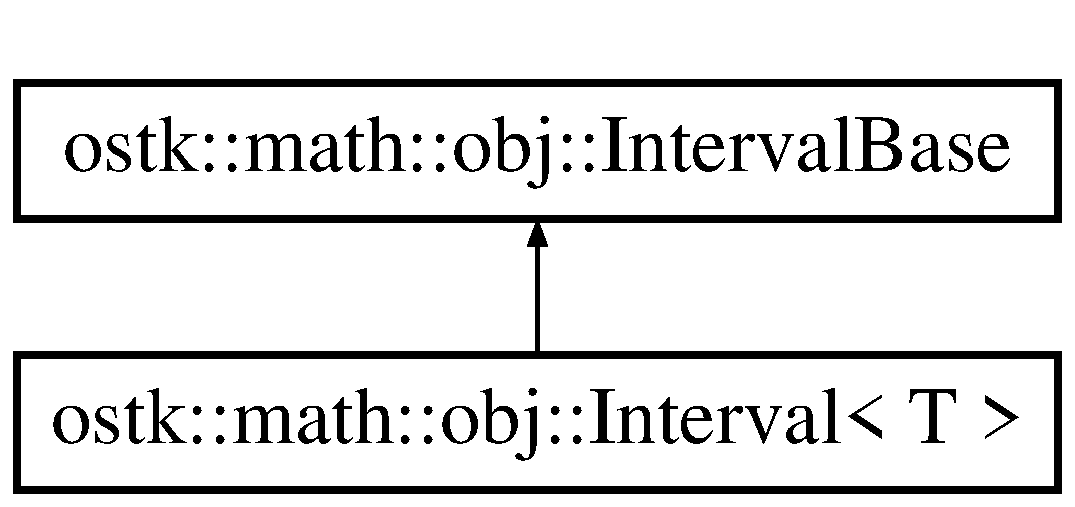
\includegraphics[height=2.000000cm]{classostk_1_1math_1_1obj_1_1_interval}
\end{center}
\end{figure}
\doxysubsection*{Public Member Functions}
\begin{DoxyCompactItemize}
\item 
\mbox{\hyperlink{classostk_1_1math_1_1obj_1_1_interval_adb3c15ff97e0097185ee7f9d2bd79a98}{Interval}} (const T \&a\+Lower\+Bound, const T \&an\+Upper\+Bound, const \mbox{\hyperlink{classostk_1_1math_1_1obj_1_1_interval_base_a0dd9bd29a9bfefa26de9b88ac81de92a}{Interval\+::\+Type}} \&an\+Interval\+Type)
\begin{DoxyCompactList}\small\item\em Constructor. \end{DoxyCompactList}\item 
bool \mbox{\hyperlink{classostk_1_1math_1_1obj_1_1_interval_a0e3495dfad73a385d27621c7969a6f49}{operator==}} (const \mbox{\hyperlink{classostk_1_1math_1_1obj_1_1_interval}{Interval}} \&an\+Interval) const
\begin{DoxyCompactList}\small\item\em Equal to operator. \end{DoxyCompactList}\item 
bool \mbox{\hyperlink{classostk_1_1math_1_1obj_1_1_interval_a7bc7fa4fb1b04aa59337ad8f2704a38d}{operator!=}} (const \mbox{\hyperlink{classostk_1_1math_1_1obj_1_1_interval}{Interval}} \&an\+Interval) const
\begin{DoxyCompactList}\small\item\em Not equal to operator. \end{DoxyCompactList}\item 
bool \mbox{\hyperlink{classostk_1_1math_1_1obj_1_1_interval_a28ed286e10ecfd77bb9145c28c9c7dff}{is\+Defined}} () const
\begin{DoxyCompactList}\small\item\em Check if interval is defined. \end{DoxyCompactList}\item 
bool \mbox{\hyperlink{classostk_1_1math_1_1obj_1_1_interval_a55edb92a6b3bfed37e60b016bd3a3e60}{is\+Degenerate}} () const
\begin{DoxyCompactList}\small\item\em Check if interval is degenerate, i.\+e. its lower and upper bounds are the equal. \end{DoxyCompactList}\item 
bool \mbox{\hyperlink{classostk_1_1math_1_1obj_1_1_interval_a58c2b405e2c5606cb774efac35bbd624}{intersects}} (const \mbox{\hyperlink{classostk_1_1math_1_1obj_1_1_interval}{Interval}} \&an\+Interval) const
\begin{DoxyCompactList}\small\item\em Check if interval is intersecting with another interval. \end{DoxyCompactList}\item 
bool \mbox{\hyperlink{classostk_1_1math_1_1obj_1_1_interval_a78acbb2eb10761ffd0f0d6198391a3fa}{contains}} (const T \&a\+Value) const
\begin{DoxyCompactList}\small\item\em Check if interval contains value. \end{DoxyCompactList}\item 
bool \mbox{\hyperlink{classostk_1_1math_1_1obj_1_1_interval_ad7d805288e161a123593991f90c437ff}{contains}} (const \mbox{\hyperlink{classostk_1_1math_1_1obj_1_1_interval}{Interval}} \&an\+Interval) const
\begin{DoxyCompactList}\small\item\em Check if interval contains another interval. \end{DoxyCompactList}\item 
const T \& \mbox{\hyperlink{classostk_1_1math_1_1obj_1_1_interval_ae2c364698fdfffb5b475da8c601c2ef9}{access\+Lower\+Bound}} () const
\begin{DoxyCompactList}\small\item\em Get reference to lower bound. \end{DoxyCompactList}\item 
const T \& \mbox{\hyperlink{classostk_1_1math_1_1obj_1_1_interval_a331c854897280447909268984716c7b2}{access\+Upper\+Bound}} () const
\begin{DoxyCompactList}\small\item\em Get reference to upper bound. \end{DoxyCompactList}\item 
\mbox{\hyperlink{classostk_1_1math_1_1obj_1_1_interval_base_a0dd9bd29a9bfefa26de9b88ac81de92a}{Interval\+::\+Type}} \mbox{\hyperlink{classostk_1_1math_1_1obj_1_1_interval_a57317128be5c1e7c4adb798149154d18}{get\+Type}} () const
\begin{DoxyCompactList}\small\item\em Get interval type. \end{DoxyCompactList}\item 
T \mbox{\hyperlink{classostk_1_1math_1_1obj_1_1_interval_ab6b044772238c2f66072377e4e6f7f25}{get\+Lower\+Bound}} () const
\begin{DoxyCompactList}\small\item\em Get lower bound. \end{DoxyCompactList}\item 
T \mbox{\hyperlink{classostk_1_1math_1_1obj_1_1_interval_a0cb57adfc1eea38a490c0c822f49602f}{get\+Upper\+Bound}} () const
\begin{DoxyCompactList}\small\item\em Get upper bound. \end{DoxyCompactList}\item 
\mbox{\hyperlink{classostk_1_1math_1_1obj_1_1_interval}{Interval}}$<$ T $>$ \mbox{\hyperlink{classostk_1_1math_1_1obj_1_1_interval_a80b12938523f90e7ec498f1cad88d244}{get\+Intersection\+With}} (const \mbox{\hyperlink{classostk_1_1math_1_1obj_1_1_interval}{Interval}} \&an\+Interval) const
\begin{DoxyCompactList}\small\item\em Get intersecting interval with another interval. \end{DoxyCompactList}\item 
\mbox{\hyperlink{classostk_1_1math_1_1obj_1_1_interval}{Interval}}$<$ T $>$ \mbox{\hyperlink{classostk_1_1math_1_1obj_1_1_interval_a3ce772da90be0c38f8357e1f24850cb5}{get\+Union\+With}} (const \mbox{\hyperlink{classostk_1_1math_1_1obj_1_1_interval}{Interval}} \&an\+Interval) const
\begin{DoxyCompactList}\small\item\em Get union interval with another interval. \end{DoxyCompactList}\item 
{\footnotesize template$<$class U $>$ }\\ctnr\+::\+Array$<$ T $>$ \mbox{\hyperlink{classostk_1_1math_1_1obj_1_1_interval_acd986bb0a03df1584b8fb6e8d5e3b13c}{generate\+Array\+With\+Step}} (const U \&a\+Step) const
\begin{DoxyCompactList}\small\item\em Generate array from a given step. \end{DoxyCompactList}\item 
ctnr\+::\+Array$<$ T $>$ \mbox{\hyperlink{classostk_1_1math_1_1obj_1_1_interval_afd8ff5687c83009802664ae953928205}{generate\+Array\+With\+Size}} (const types\+::\+Size \&an\+Array\+Size) const
\begin{DoxyCompactList}\small\item\em Generate array with a given size. \end{DoxyCompactList}\item 
types\+::\+String \mbox{\hyperlink{classostk_1_1math_1_1obj_1_1_interval_ab467cbf6bc51f3adefa75f0667a7b26c}{to\+String}} () const
\begin{DoxyCompactList}\small\item\em Get serialized interval. \end{DoxyCompactList}\item 
void \mbox{\hyperlink{classostk_1_1math_1_1obj_1_1_interval_a84876dff7017bf9ebb5c7ef71aefffc7}{set\+Type}} (const \mbox{\hyperlink{classostk_1_1math_1_1obj_1_1_interval_base_a0dd9bd29a9bfefa26de9b88ac81de92a}{Interval\+::\+Type}} \&a\+Type)
\begin{DoxyCompactList}\small\item\em \mbox{\hyperlink{classostk_1_1math_1_1obj_1_1_interval}{Interval}} type setter. \end{DoxyCompactList}\item 
void \mbox{\hyperlink{classostk_1_1math_1_1obj_1_1_interval_a958544f14f36300f89e383351279299d}{set\+Lower\+Bound}} (const T \&a\+Lower\+Bound)
\begin{DoxyCompactList}\small\item\em \mbox{\hyperlink{classostk_1_1math_1_1obj_1_1_interval}{Interval}} lower bound setter. \end{DoxyCompactList}\item 
void \mbox{\hyperlink{classostk_1_1math_1_1obj_1_1_interval_a5e53477bc77dea2587283a1fa73b3659}{set\+Upper\+Bound}} (const T \&an\+Upper\+Bound)
\begin{DoxyCompactList}\small\item\em \mbox{\hyperlink{classostk_1_1math_1_1obj_1_1_interval}{Interval}} upper bound setter. \end{DoxyCompactList}\end{DoxyCompactItemize}
\doxysubsection*{Static Public Member Functions}
\begin{DoxyCompactItemize}
\item 
static \mbox{\hyperlink{classostk_1_1math_1_1obj_1_1_interval}{Interval}}$<$ T $>$ \mbox{\hyperlink{classostk_1_1math_1_1obj_1_1_interval_a34149197805573678f6ed5d29679be88}{Undefined}} ()
\begin{DoxyCompactList}\small\item\em Constructs an undefined interval. \end{DoxyCompactList}\item 
static \mbox{\hyperlink{classostk_1_1math_1_1obj_1_1_interval}{Interval}}$<$ T $>$ \mbox{\hyperlink{classostk_1_1math_1_1obj_1_1_interval_a48e9f436e8994c49026a1ecd503bc190}{Closed}} (const T \&a\+Lower\+Bound, const T \&an\+Upper\+Bound)
\begin{DoxyCompactList}\small\item\em Constructs a closed interval. \end{DoxyCompactList}\item 
static \mbox{\hyperlink{classostk_1_1math_1_1obj_1_1_interval}{Interval}}$<$ T $>$ \mbox{\hyperlink{classostk_1_1math_1_1obj_1_1_interval_ac80686dee5b2893e7b74a5120340db99}{Open}} (const T \&a\+Lower\+Bound, const T \&an\+Upper\+Bound)
\begin{DoxyCompactList}\small\item\em Constructs an open interval. \end{DoxyCompactList}\item 
static \mbox{\hyperlink{classostk_1_1math_1_1obj_1_1_interval}{Interval}}$<$ T $>$ \mbox{\hyperlink{classostk_1_1math_1_1obj_1_1_interval_a47bfd73591e68d8c1c7ff1fd626cbf5b}{Half\+Open\+Left}} (const T \&a\+Lower\+Bound, const T \&an\+Upper\+Bound)
\begin{DoxyCompactList}\small\item\em Constructs an half-\/open left interval. \end{DoxyCompactList}\item 
static \mbox{\hyperlink{classostk_1_1math_1_1obj_1_1_interval}{Interval}}$<$ T $>$ \mbox{\hyperlink{classostk_1_1math_1_1obj_1_1_interval_abe98617b87988bf157703cbd04bb1905}{Half\+Open\+Right}} (const T \&a\+Lower\+Bound, const T \&an\+Upper\+Bound)
\begin{DoxyCompactList}\small\item\em Constructs an half-\/open right interval. \end{DoxyCompactList}\item 
static \mbox{\hyperlink{classostk_1_1math_1_1obj_1_1_interval}{Interval}}$<$ T $>$ \mbox{\hyperlink{classostk_1_1math_1_1obj_1_1_interval_a8013b6fe2914101612ae83ee815110e4}{Parse}} (const types\+::\+String \&a\+String)
\begin{DoxyCompactList}\small\item\em Constructs an interval from a given string. \end{DoxyCompactList}\item 
static types\+::\+String \mbox{\hyperlink{classostk_1_1math_1_1obj_1_1_interval_abe58217bb3d134390c49652e53e2e57e}{String\+From\+Type}} (const \mbox{\hyperlink{classostk_1_1math_1_1obj_1_1_interval_base_a0dd9bd29a9bfefa26de9b88ac81de92a}{Interval\+::\+Type}} \&an\+Interval\+Type)
\begin{DoxyCompactList}\small\item\em Converts interval type to string. \end{DoxyCompactList}\end{DoxyCompactItemize}
\doxysubsection*{Friends}
\begin{DoxyCompactItemize}
\item 
{\footnotesize template$<$class U $>$ }\\std\+::ostream \& \mbox{\hyperlink{classostk_1_1math_1_1obj_1_1_interval_a3aa32afa8cb5d85eeb45540b0bf5657b}{operator$<$$<$}} (std\+::ostream \&an\+Output\+Stream, const \mbox{\hyperlink{classostk_1_1math_1_1obj_1_1_interval}{Interval}}$<$ U $>$ \&an\+Interval)
\begin{DoxyCompactList}\small\item\em Output stream operator. \end{DoxyCompactList}\end{DoxyCompactItemize}
\doxysubsection*{Additional Inherited Members}


\doxysubsection{Detailed Description}
\subsubsection*{template$<$class T$>$\newline
class ostk\+::math\+::obj\+::\+Interval$<$ T $>$}

Set of numbers with the property that any number that lies between two numbers in the set is also included in the set. 

\href{https://en.wikipedia.org/wiki/Interval_}{\texttt{ https\+://en.\+wikipedia.\+org/wiki/\+Interval\+\_\+}}(mathematics) 

\doxysubsection{Constructor \& Destructor Documentation}
\mbox{\Hypertarget{classostk_1_1math_1_1obj_1_1_interval_adb3c15ff97e0097185ee7f9d2bd79a98}\label{classostk_1_1math_1_1obj_1_1_interval_adb3c15ff97e0097185ee7f9d2bd79a98}} 
\index{ostk::math::obj::Interval$<$ T $>$@{ostk::math::obj::Interval$<$ T $>$}!Interval@{Interval}}
\index{Interval@{Interval}!ostk::math::obj::Interval$<$ T $>$@{ostk::math::obj::Interval$<$ T $>$}}
\doxysubsubsection{\texorpdfstring{Interval()}{Interval()}}
{\footnotesize\ttfamily template$<$class T $>$ \\
\mbox{\hyperlink{classostk_1_1math_1_1obj_1_1_interval}{ostk\+::math\+::obj\+::\+Interval}}$<$ T $>$\+::\mbox{\hyperlink{classostk_1_1math_1_1obj_1_1_interval}{Interval}} (\begin{DoxyParamCaption}\item[{const T \&}]{a\+Lower\+Bound,  }\item[{const T \&}]{an\+Upper\+Bound,  }\item[{const \mbox{\hyperlink{classostk_1_1math_1_1obj_1_1_interval}{Interval}}$<$ T $>$\+::\mbox{\hyperlink{classostk_1_1math_1_1obj_1_1_interval_base_a0dd9bd29a9bfefa26de9b88ac81de92a}{Type}} \&}]{an\+Interval\+Type }\end{DoxyParamCaption})}



Constructor. 


\begin{DoxyCode}{0}
\DoxyCodeLine{Interval<Real> interval(0.0, 1.0, \mbox{\hyperlink{classostk_1_1math_1_1obj_1_1_interval_base_a0dd9bd29a9bfefa26de9b88ac81de92aa03f4a47830f97377a35321051685071e}{Interval::Type::Closed}}) ;}
\end{DoxyCode}



\begin{DoxyParams}[1]{Parameters}
\mbox{\texttt{ in}}  & {\em a\+Lower\+Bound} & A lower bound \\
\hline
\mbox{\texttt{ in}}  & {\em an\+Upper\+Bound} & An upper bound \\
\hline
\mbox{\texttt{ in}}  & {\em an\+Interval\+Type} & An interval type \\
\hline
\end{DoxyParams}


\doxysubsection{Member Function Documentation}
\mbox{\Hypertarget{classostk_1_1math_1_1obj_1_1_interval_ae2c364698fdfffb5b475da8c601c2ef9}\label{classostk_1_1math_1_1obj_1_1_interval_ae2c364698fdfffb5b475da8c601c2ef9}} 
\index{ostk::math::obj::Interval$<$ T $>$@{ostk::math::obj::Interval$<$ T $>$}!accessLowerBound@{accessLowerBound}}
\index{accessLowerBound@{accessLowerBound}!ostk::math::obj::Interval$<$ T $>$@{ostk::math::obj::Interval$<$ T $>$}}
\doxysubsubsection{\texorpdfstring{accessLowerBound()}{accessLowerBound()}}
{\footnotesize\ttfamily template$<$class T $>$ \\
const T\& \mbox{\hyperlink{classostk_1_1math_1_1obj_1_1_interval}{ostk\+::math\+::obj\+::\+Interval}}$<$ T $>$\+::access\+Lower\+Bound (\begin{DoxyParamCaption}{ }\end{DoxyParamCaption}) const}



Get reference to lower bound. 


\begin{DoxyCode}{0}
\DoxyCodeLine{Interval<Real> interval = \mbox{\hyperlink{classostk_1_1math_1_1obj_1_1_interval_a48e9f436e8994c49026a1ecd503bc190}{Interval<Real>::Closed}}(0.0, 1.0) ;}
\DoxyCodeLine{interval.accessLowerBound() ; \textcolor{comment}{// \&0.0}}
\end{DoxyCode}


\begin{DoxyReturn}{Returns}
Reference to lower bound 
\end{DoxyReturn}
\mbox{\Hypertarget{classostk_1_1math_1_1obj_1_1_interval_a331c854897280447909268984716c7b2}\label{classostk_1_1math_1_1obj_1_1_interval_a331c854897280447909268984716c7b2}} 
\index{ostk::math::obj::Interval$<$ T $>$@{ostk::math::obj::Interval$<$ T $>$}!accessUpperBound@{accessUpperBound}}
\index{accessUpperBound@{accessUpperBound}!ostk::math::obj::Interval$<$ T $>$@{ostk::math::obj::Interval$<$ T $>$}}
\doxysubsubsection{\texorpdfstring{accessUpperBound()}{accessUpperBound()}}
{\footnotesize\ttfamily template$<$class T $>$ \\
const T\& \mbox{\hyperlink{classostk_1_1math_1_1obj_1_1_interval}{ostk\+::math\+::obj\+::\+Interval}}$<$ T $>$\+::access\+Upper\+Bound (\begin{DoxyParamCaption}{ }\end{DoxyParamCaption}) const}



Get reference to upper bound. 


\begin{DoxyCode}{0}
\DoxyCodeLine{Interval<Real> interval = \mbox{\hyperlink{classostk_1_1math_1_1obj_1_1_interval_a48e9f436e8994c49026a1ecd503bc190}{Interval<Real>::Closed}}(0.0, 1.0) ;}
\DoxyCodeLine{interval.accessUpperBound() ; \textcolor{comment}{// \&1.0}}
\end{DoxyCode}


\begin{DoxyReturn}{Returns}
Reference to upper bound 
\end{DoxyReturn}
\mbox{\Hypertarget{classostk_1_1math_1_1obj_1_1_interval_a48e9f436e8994c49026a1ecd503bc190}\label{classostk_1_1math_1_1obj_1_1_interval_a48e9f436e8994c49026a1ecd503bc190}} 
\index{ostk::math::obj::Interval$<$ T $>$@{ostk::math::obj::Interval$<$ T $>$}!Closed@{Closed}}
\index{Closed@{Closed}!ostk::math::obj::Interval$<$ T $>$@{ostk::math::obj::Interval$<$ T $>$}}
\doxysubsubsection{\texorpdfstring{Closed()}{Closed()}}
{\footnotesize\ttfamily template$<$class T $>$ \\
static \mbox{\hyperlink{classostk_1_1math_1_1obj_1_1_interval}{Interval}}$<$T$>$ \mbox{\hyperlink{classostk_1_1math_1_1obj_1_1_interval}{ostk\+::math\+::obj\+::\+Interval}}$<$ T $>$\+::Closed (\begin{DoxyParamCaption}\item[{const T \&}]{a\+Lower\+Bound,  }\item[{const T \&}]{an\+Upper\+Bound }\end{DoxyParamCaption})\hspace{0.3cm}{\ttfamily [static]}}



Constructs a closed interval. 


\begin{DoxyCode}{0}
\DoxyCodeLine{Interval<Real> interval = \mbox{\hyperlink{classostk_1_1math_1_1obj_1_1_interval_a48e9f436e8994c49026a1ecd503bc190}{Interval<Real>::Closed}}(0.0, 1.0) ; \textcolor{comment}{// [0.0, 1.0]}}
\end{DoxyCode}


\begin{DoxyReturn}{Returns}
Closed interval 
\end{DoxyReturn}
\mbox{\Hypertarget{classostk_1_1math_1_1obj_1_1_interval_ad7d805288e161a123593991f90c437ff}\label{classostk_1_1math_1_1obj_1_1_interval_ad7d805288e161a123593991f90c437ff}} 
\index{ostk::math::obj::Interval$<$ T $>$@{ostk::math::obj::Interval$<$ T $>$}!contains@{contains}}
\index{contains@{contains}!ostk::math::obj::Interval$<$ T $>$@{ostk::math::obj::Interval$<$ T $>$}}
\doxysubsubsection{\texorpdfstring{contains()}{contains()}\hspace{0.1cm}{\footnotesize\ttfamily [1/2]}}
{\footnotesize\ttfamily template$<$class T $>$ \\
bool \mbox{\hyperlink{classostk_1_1math_1_1obj_1_1_interval}{ostk\+::math\+::obj\+::\+Interval}}$<$ T $>$\+::contains (\begin{DoxyParamCaption}\item[{const \mbox{\hyperlink{classostk_1_1math_1_1obj_1_1_interval}{Interval}}$<$ T $>$ \&}]{an\+Interval }\end{DoxyParamCaption}) const}



Check if interval contains another interval. 


\begin{DoxyCode}{0}
\DoxyCodeLine{\mbox{\hyperlink{classostk_1_1math_1_1obj_1_1_interval_a48e9f436e8994c49026a1ecd503bc190}{Interval<Real>::Closed}}(0.0, 1.0).contains(\mbox{\hyperlink{classostk_1_1math_1_1obj_1_1_interval_ac80686dee5b2893e7b74a5120340db99}{Interval<Real>::Open}}(0.2, 0.8)) ; \textcolor{comment}{// True}}
\end{DoxyCode}



\begin{DoxyParams}[1]{Parameters}
\mbox{\texttt{ in}}  & {\em an\+Interval} & An interval \\
\hline
\end{DoxyParams}
\begin{DoxyReturn}{Returns}
True if interval contains another interval 
\end{DoxyReturn}
\mbox{\Hypertarget{classostk_1_1math_1_1obj_1_1_interval_a78acbb2eb10761ffd0f0d6198391a3fa}\label{classostk_1_1math_1_1obj_1_1_interval_a78acbb2eb10761ffd0f0d6198391a3fa}} 
\index{ostk::math::obj::Interval$<$ T $>$@{ostk::math::obj::Interval$<$ T $>$}!contains@{contains}}
\index{contains@{contains}!ostk::math::obj::Interval$<$ T $>$@{ostk::math::obj::Interval$<$ T $>$}}
\doxysubsubsection{\texorpdfstring{contains()}{contains()}\hspace{0.1cm}{\footnotesize\ttfamily [2/2]}}
{\footnotesize\ttfamily template$<$class T $>$ \\
bool \mbox{\hyperlink{classostk_1_1math_1_1obj_1_1_interval}{ostk\+::math\+::obj\+::\+Interval}}$<$ T $>$\+::contains (\begin{DoxyParamCaption}\item[{const T \&}]{a\+Value }\end{DoxyParamCaption}) const}



Check if interval contains value. 


\begin{DoxyCode}{0}
\DoxyCodeLine{\mbox{\hyperlink{classostk_1_1math_1_1obj_1_1_interval_a48e9f436e8994c49026a1ecd503bc190}{Interval<Real>::Closed}}(0.0, 1.0).contains(0.5) ; \textcolor{comment}{// True}}
\end{DoxyCode}



\begin{DoxyParams}[1]{Parameters}
\mbox{\texttt{ in}}  & {\em a\+Value} & A value \\
\hline
\end{DoxyParams}
\begin{DoxyReturn}{Returns}
True if interval contains value 
\end{DoxyReturn}
\mbox{\Hypertarget{classostk_1_1math_1_1obj_1_1_interval_afd8ff5687c83009802664ae953928205}\label{classostk_1_1math_1_1obj_1_1_interval_afd8ff5687c83009802664ae953928205}} 
\index{ostk::math::obj::Interval$<$ T $>$@{ostk::math::obj::Interval$<$ T $>$}!generateArrayWithSize@{generateArrayWithSize}}
\index{generateArrayWithSize@{generateArrayWithSize}!ostk::math::obj::Interval$<$ T $>$@{ostk::math::obj::Interval$<$ T $>$}}
\doxysubsubsection{\texorpdfstring{generateArrayWithSize()}{generateArrayWithSize()}}
{\footnotesize\ttfamily template$<$class T $>$ \\
ctnr\+::\+Array$<$T$>$ \mbox{\hyperlink{classostk_1_1math_1_1obj_1_1_interval}{ostk\+::math\+::obj\+::\+Interval}}$<$ T $>$\+::generate\+Array\+With\+Size (\begin{DoxyParamCaption}\item[{const types\+::\+Size \&}]{an\+Array\+Size }\end{DoxyParamCaption}) const}



Generate array with a given size. 


\begin{DoxyCode}{0}
\DoxyCodeLine{Interval<Real> interval = \mbox{\hyperlink{classostk_1_1math_1_1obj_1_1_interval_a48e9f436e8994c49026a1ecd503bc190}{Interval<Real>::Closed}}(0.0, 1.0) ;}
\DoxyCodeLine{Array<Real> array = interval.generateArrayWithSize(3) ; \textcolor{comment}{// [0.0, 0.5, 1.0]}}
\end{DoxyCode}



\begin{DoxyParams}[1]{Parameters}
\mbox{\texttt{ in}}  & {\em an\+Array\+Size} & An array size \\
\hline
\end{DoxyParams}
\begin{DoxyReturn}{Returns}
Array of values 
\end{DoxyReturn}
\mbox{\Hypertarget{classostk_1_1math_1_1obj_1_1_interval_acd986bb0a03df1584b8fb6e8d5e3b13c}\label{classostk_1_1math_1_1obj_1_1_interval_acd986bb0a03df1584b8fb6e8d5e3b13c}} 
\index{ostk::math::obj::Interval$<$ T $>$@{ostk::math::obj::Interval$<$ T $>$}!generateArrayWithStep@{generateArrayWithStep}}
\index{generateArrayWithStep@{generateArrayWithStep}!ostk::math::obj::Interval$<$ T $>$@{ostk::math::obj::Interval$<$ T $>$}}
\doxysubsubsection{\texorpdfstring{generateArrayWithStep()}{generateArrayWithStep()}}
{\footnotesize\ttfamily template$<$class T $>$ \\
template$<$class U $>$ \\
ctnr\+::\+Array$<$T$>$ \mbox{\hyperlink{classostk_1_1math_1_1obj_1_1_interval}{ostk\+::math\+::obj\+::\+Interval}}$<$ T $>$\+::generate\+Array\+With\+Step (\begin{DoxyParamCaption}\item[{const U \&}]{a\+Step }\end{DoxyParamCaption}) const}



Generate array from a given step. 


\begin{DoxyCode}{0}
\DoxyCodeLine{Interval<Real> interval = \mbox{\hyperlink{classostk_1_1math_1_1obj_1_1_interval_a48e9f436e8994c49026a1ecd503bc190}{Interval<Real>::Closed}}(0.0, 1.0) ;}
\DoxyCodeLine{Array<Real> array = interval.generateArrayWithStep(0.5) ; \textcolor{comment}{// [0.0, 0.5, 1.0]}}
\end{DoxyCode}



\begin{DoxyParams}[1]{Parameters}
\mbox{\texttt{ in}}  & {\em a\+Step} & A step \\
\hline
\end{DoxyParams}
\begin{DoxyReturn}{Returns}
Array of values 
\end{DoxyReturn}
\mbox{\Hypertarget{classostk_1_1math_1_1obj_1_1_interval_a80b12938523f90e7ec498f1cad88d244}\label{classostk_1_1math_1_1obj_1_1_interval_a80b12938523f90e7ec498f1cad88d244}} 
\index{ostk::math::obj::Interval$<$ T $>$@{ostk::math::obj::Interval$<$ T $>$}!getIntersectionWith@{getIntersectionWith}}
\index{getIntersectionWith@{getIntersectionWith}!ostk::math::obj::Interval$<$ T $>$@{ostk::math::obj::Interval$<$ T $>$}}
\doxysubsubsection{\texorpdfstring{getIntersectionWith()}{getIntersectionWith()}}
{\footnotesize\ttfamily template$<$class T $>$ \\
\mbox{\hyperlink{classostk_1_1math_1_1obj_1_1_interval}{Interval}}$<$T$>$ \mbox{\hyperlink{classostk_1_1math_1_1obj_1_1_interval}{ostk\+::math\+::obj\+::\+Interval}}$<$ T $>$\+::get\+Intersection\+With (\begin{DoxyParamCaption}\item[{const \mbox{\hyperlink{classostk_1_1math_1_1obj_1_1_interval}{Interval}}$<$ T $>$ \&}]{an\+Interval }\end{DoxyParamCaption}) const}



Get intersecting interval with another interval. 


\begin{DoxyCode}{0}
\DoxyCodeLine{Interval<Real> firstInterval = \mbox{\hyperlink{classostk_1_1math_1_1obj_1_1_interval_a48e9f436e8994c49026a1ecd503bc190}{Interval<Real>::Closed}}(0.0, 1.0) ;}
\DoxyCodeLine{Interval<Real> secondInterval = \mbox{\hyperlink{classostk_1_1math_1_1obj_1_1_interval_a48e9f436e8994c49026a1ecd503bc190}{Interval<Real>::Closed}}(0.5, 1.5) ;}
\DoxyCodeLine{Interval<Real> intersection = firstInterval.getIntersectionWith(secondInterval) ; \textcolor{comment}{//}}
\DoxyCodeLine{[0.5, 1.0]}
\end{DoxyCode}



\begin{DoxyParams}[1]{Parameters}
\mbox{\texttt{ in}}  & {\em an\+Interval} & An interval \\
\hline
\end{DoxyParams}
\begin{DoxyReturn}{Returns}
Intersecting interval 
\end{DoxyReturn}
\mbox{\Hypertarget{classostk_1_1math_1_1obj_1_1_interval_ab6b044772238c2f66072377e4e6f7f25}\label{classostk_1_1math_1_1obj_1_1_interval_ab6b044772238c2f66072377e4e6f7f25}} 
\index{ostk::math::obj::Interval$<$ T $>$@{ostk::math::obj::Interval$<$ T $>$}!getLowerBound@{getLowerBound}}
\index{getLowerBound@{getLowerBound}!ostk::math::obj::Interval$<$ T $>$@{ostk::math::obj::Interval$<$ T $>$}}
\doxysubsubsection{\texorpdfstring{getLowerBound()}{getLowerBound()}}
{\footnotesize\ttfamily template$<$class T $>$ \\
T \mbox{\hyperlink{classostk_1_1math_1_1obj_1_1_interval}{ostk\+::math\+::obj\+::\+Interval}}$<$ T $>$\+::get\+Lower\+Bound (\begin{DoxyParamCaption}{ }\end{DoxyParamCaption}) const}



Get lower bound. 


\begin{DoxyCode}{0}
\DoxyCodeLine{Interval<Real> interval = \mbox{\hyperlink{classostk_1_1math_1_1obj_1_1_interval_a48e9f436e8994c49026a1ecd503bc190}{Interval<Real>::Closed}}(0.0, 1.0) ;}
\DoxyCodeLine{interval.getLowerBound() ; \textcolor{comment}{// 0.0}}
\end{DoxyCode}


\begin{DoxyReturn}{Returns}
Lower bound 
\end{DoxyReturn}
\mbox{\Hypertarget{classostk_1_1math_1_1obj_1_1_interval_a57317128be5c1e7c4adb798149154d18}\label{classostk_1_1math_1_1obj_1_1_interval_a57317128be5c1e7c4adb798149154d18}} 
\index{ostk::math::obj::Interval$<$ T $>$@{ostk::math::obj::Interval$<$ T $>$}!getType@{getType}}
\index{getType@{getType}!ostk::math::obj::Interval$<$ T $>$@{ostk::math::obj::Interval$<$ T $>$}}
\doxysubsubsection{\texorpdfstring{getType()}{getType()}}
{\footnotesize\ttfamily template$<$class T $>$ \\
\mbox{\hyperlink{classostk_1_1math_1_1obj_1_1_interval_base_a0dd9bd29a9bfefa26de9b88ac81de92a}{Interval\+::\+Type}} \mbox{\hyperlink{classostk_1_1math_1_1obj_1_1_interval}{ostk\+::math\+::obj\+::\+Interval}}$<$ T $>$\+::get\+Type (\begin{DoxyParamCaption}{ }\end{DoxyParamCaption}) const}



Get interval type. 


\begin{DoxyCode}{0}
\DoxyCodeLine{Interval<Real> interval = \mbox{\hyperlink{classostk_1_1math_1_1obj_1_1_interval_a48e9f436e8994c49026a1ecd503bc190}{Interval<Real>::Closed}}(0.0, 1.0) ;}
\DoxyCodeLine{interval.getType() ; \textcolor{comment}{// Interval<Real>::Type::Closed}}
\end{DoxyCode}


\begin{DoxyReturn}{Returns}
\mbox{\hyperlink{classostk_1_1math_1_1obj_1_1_interval}{Interval}} type 
\end{DoxyReturn}
\mbox{\Hypertarget{classostk_1_1math_1_1obj_1_1_interval_a3ce772da90be0c38f8357e1f24850cb5}\label{classostk_1_1math_1_1obj_1_1_interval_a3ce772da90be0c38f8357e1f24850cb5}} 
\index{ostk::math::obj::Interval$<$ T $>$@{ostk::math::obj::Interval$<$ T $>$}!getUnionWith@{getUnionWith}}
\index{getUnionWith@{getUnionWith}!ostk::math::obj::Interval$<$ T $>$@{ostk::math::obj::Interval$<$ T $>$}}
\doxysubsubsection{\texorpdfstring{getUnionWith()}{getUnionWith()}}
{\footnotesize\ttfamily template$<$class T $>$ \\
\mbox{\hyperlink{classostk_1_1math_1_1obj_1_1_interval}{Interval}}$<$T$>$ \mbox{\hyperlink{classostk_1_1math_1_1obj_1_1_interval}{ostk\+::math\+::obj\+::\+Interval}}$<$ T $>$\+::get\+Union\+With (\begin{DoxyParamCaption}\item[{const \mbox{\hyperlink{classostk_1_1math_1_1obj_1_1_interval}{Interval}}$<$ T $>$ \&}]{an\+Interval }\end{DoxyParamCaption}) const}



Get union interval with another interval. 


\begin{DoxyCode}{0}
\DoxyCodeLine{Interval<Real> firstInterval = \mbox{\hyperlink{classostk_1_1math_1_1obj_1_1_interval_a48e9f436e8994c49026a1ecd503bc190}{Interval<Real>::Closed}}(0.0, 1.0) ;}
\DoxyCodeLine{Interval<Real> secondInterval = \mbox{\hyperlink{classostk_1_1math_1_1obj_1_1_interval_a48e9f436e8994c49026a1ecd503bc190}{Interval<Real>::Closed}}(0.5, 1.5) ;}
\DoxyCodeLine{Interval<Real> \textcolor{keyword}{union }= firstInterval.getUnionWith(secondInterval) ; \textcolor{comment}{// [0.0, 1.5]}}
\end{DoxyCode}



\begin{DoxyParams}[1]{Parameters}
\mbox{\texttt{ in}}  & {\em an\+Interval} & An interval \\
\hline
\end{DoxyParams}
\begin{DoxyReturn}{Returns}
Union interval 
\end{DoxyReturn}
\mbox{\Hypertarget{classostk_1_1math_1_1obj_1_1_interval_a0cb57adfc1eea38a490c0c822f49602f}\label{classostk_1_1math_1_1obj_1_1_interval_a0cb57adfc1eea38a490c0c822f49602f}} 
\index{ostk::math::obj::Interval$<$ T $>$@{ostk::math::obj::Interval$<$ T $>$}!getUpperBound@{getUpperBound}}
\index{getUpperBound@{getUpperBound}!ostk::math::obj::Interval$<$ T $>$@{ostk::math::obj::Interval$<$ T $>$}}
\doxysubsubsection{\texorpdfstring{getUpperBound()}{getUpperBound()}}
{\footnotesize\ttfamily template$<$class T $>$ \\
T \mbox{\hyperlink{classostk_1_1math_1_1obj_1_1_interval}{ostk\+::math\+::obj\+::\+Interval}}$<$ T $>$\+::get\+Upper\+Bound (\begin{DoxyParamCaption}{ }\end{DoxyParamCaption}) const}



Get upper bound. 


\begin{DoxyCode}{0}
\DoxyCodeLine{Interval<Real> interval = \mbox{\hyperlink{classostk_1_1math_1_1obj_1_1_interval_a48e9f436e8994c49026a1ecd503bc190}{Interval<Real>::Closed}}(0.0, 1.0) ;}
\DoxyCodeLine{interval.getUpperBound() ; \textcolor{comment}{// 1.0}}
\end{DoxyCode}


\begin{DoxyReturn}{Returns}
Upper bound 
\end{DoxyReturn}
\mbox{\Hypertarget{classostk_1_1math_1_1obj_1_1_interval_a47bfd73591e68d8c1c7ff1fd626cbf5b}\label{classostk_1_1math_1_1obj_1_1_interval_a47bfd73591e68d8c1c7ff1fd626cbf5b}} 
\index{ostk::math::obj::Interval$<$ T $>$@{ostk::math::obj::Interval$<$ T $>$}!HalfOpenLeft@{HalfOpenLeft}}
\index{HalfOpenLeft@{HalfOpenLeft}!ostk::math::obj::Interval$<$ T $>$@{ostk::math::obj::Interval$<$ T $>$}}
\doxysubsubsection{\texorpdfstring{HalfOpenLeft()}{HalfOpenLeft()}}
{\footnotesize\ttfamily template$<$class T $>$ \\
static \mbox{\hyperlink{classostk_1_1math_1_1obj_1_1_interval}{Interval}}$<$T$>$ \mbox{\hyperlink{classostk_1_1math_1_1obj_1_1_interval}{ostk\+::math\+::obj\+::\+Interval}}$<$ T $>$\+::Half\+Open\+Left (\begin{DoxyParamCaption}\item[{const T \&}]{a\+Lower\+Bound,  }\item[{const T \&}]{an\+Upper\+Bound }\end{DoxyParamCaption})\hspace{0.3cm}{\ttfamily [static]}}



Constructs an half-\/open left interval. 


\begin{DoxyCode}{0}
\DoxyCodeLine{Interval<Real> interval = \mbox{\hyperlink{classostk_1_1math_1_1obj_1_1_interval_a47bfd73591e68d8c1c7ff1fd626cbf5b}{Interval<Real>::HalfOpenLeft}}(0.0, 1.0) ; \textcolor{comment}{// ]0.0, 1.0]}}
\end{DoxyCode}


\begin{DoxyReturn}{Returns}
Half-\/open left interval 
\end{DoxyReturn}
\mbox{\Hypertarget{classostk_1_1math_1_1obj_1_1_interval_abe98617b87988bf157703cbd04bb1905}\label{classostk_1_1math_1_1obj_1_1_interval_abe98617b87988bf157703cbd04bb1905}} 
\index{ostk::math::obj::Interval$<$ T $>$@{ostk::math::obj::Interval$<$ T $>$}!HalfOpenRight@{HalfOpenRight}}
\index{HalfOpenRight@{HalfOpenRight}!ostk::math::obj::Interval$<$ T $>$@{ostk::math::obj::Interval$<$ T $>$}}
\doxysubsubsection{\texorpdfstring{HalfOpenRight()}{HalfOpenRight()}}
{\footnotesize\ttfamily template$<$class T $>$ \\
static \mbox{\hyperlink{classostk_1_1math_1_1obj_1_1_interval}{Interval}}$<$T$>$ \mbox{\hyperlink{classostk_1_1math_1_1obj_1_1_interval}{ostk\+::math\+::obj\+::\+Interval}}$<$ T $>$\+::Half\+Open\+Right (\begin{DoxyParamCaption}\item[{const T \&}]{a\+Lower\+Bound,  }\item[{const T \&}]{an\+Upper\+Bound }\end{DoxyParamCaption})\hspace{0.3cm}{\ttfamily [static]}}



Constructs an half-\/open right interval. 


\begin{DoxyCode}{0}
\DoxyCodeLine{Interval<Real> interval = \mbox{\hyperlink{classostk_1_1math_1_1obj_1_1_interval_abe98617b87988bf157703cbd04bb1905}{Interval<Real>::HalfOpenRight}}(0.0, 1.0) ; \textcolor{comment}{// [0.0, 1.0[}}
\end{DoxyCode}


\begin{DoxyReturn}{Returns}
Half-\/open right interval 
\end{DoxyReturn}
\mbox{\Hypertarget{classostk_1_1math_1_1obj_1_1_interval_a58c2b405e2c5606cb774efac35bbd624}\label{classostk_1_1math_1_1obj_1_1_interval_a58c2b405e2c5606cb774efac35bbd624}} 
\index{ostk::math::obj::Interval$<$ T $>$@{ostk::math::obj::Interval$<$ T $>$}!intersects@{intersects}}
\index{intersects@{intersects}!ostk::math::obj::Interval$<$ T $>$@{ostk::math::obj::Interval$<$ T $>$}}
\doxysubsubsection{\texorpdfstring{intersects()}{intersects()}}
{\footnotesize\ttfamily template$<$class T $>$ \\
bool \mbox{\hyperlink{classostk_1_1math_1_1obj_1_1_interval}{ostk\+::math\+::obj\+::\+Interval}}$<$ T $>$\+::intersects (\begin{DoxyParamCaption}\item[{const \mbox{\hyperlink{classostk_1_1math_1_1obj_1_1_interval}{Interval}}$<$ T $>$ \&}]{an\+Interval }\end{DoxyParamCaption}) const}



Check if interval is intersecting with another interval. 


\begin{DoxyCode}{0}
\DoxyCodeLine{\mbox{\hyperlink{classostk_1_1math_1_1obj_1_1_interval_a48e9f436e8994c49026a1ecd503bc190}{Interval<Real>::Closed}}(0.0, 1.0).intersects(\mbox{\hyperlink{classostk_1_1math_1_1obj_1_1_interval_a48e9f436e8994c49026a1ecd503bc190}{Interval<Real>::Closed}}(0.5, 1.5)) ; \textcolor{comment}{// True}}
\end{DoxyCode}



\begin{DoxyParams}[1]{Parameters}
\mbox{\texttt{ in}}  & {\em an\+Interval} & An interval \\
\hline
\end{DoxyParams}
\begin{DoxyReturn}{Returns}
True if intervals are intersecting 
\end{DoxyReturn}
\mbox{\Hypertarget{classostk_1_1math_1_1obj_1_1_interval_a28ed286e10ecfd77bb9145c28c9c7dff}\label{classostk_1_1math_1_1obj_1_1_interval_a28ed286e10ecfd77bb9145c28c9c7dff}} 
\index{ostk::math::obj::Interval$<$ T $>$@{ostk::math::obj::Interval$<$ T $>$}!isDefined@{isDefined}}
\index{isDefined@{isDefined}!ostk::math::obj::Interval$<$ T $>$@{ostk::math::obj::Interval$<$ T $>$}}
\doxysubsubsection{\texorpdfstring{isDefined()}{isDefined()}}
{\footnotesize\ttfamily template$<$class T $>$ \\
bool \mbox{\hyperlink{classostk_1_1math_1_1obj_1_1_interval}{ostk\+::math\+::obj\+::\+Interval}}$<$ T $>$\+::is\+Defined (\begin{DoxyParamCaption}{ }\end{DoxyParamCaption}) const}



Check if interval is defined. 


\begin{DoxyCode}{0}
\DoxyCodeLine{\mbox{\hyperlink{classostk_1_1math_1_1obj_1_1_interval_a48e9f436e8994c49026a1ecd503bc190}{Interval<Real>::Closed}}(0.0, 1.0).isDefined() ; \textcolor{comment}{// True}}
\end{DoxyCode}


\begin{DoxyReturn}{Returns}
True if interval is defined 
\end{DoxyReturn}
\mbox{\Hypertarget{classostk_1_1math_1_1obj_1_1_interval_a55edb92a6b3bfed37e60b016bd3a3e60}\label{classostk_1_1math_1_1obj_1_1_interval_a55edb92a6b3bfed37e60b016bd3a3e60}} 
\index{ostk::math::obj::Interval$<$ T $>$@{ostk::math::obj::Interval$<$ T $>$}!isDegenerate@{isDegenerate}}
\index{isDegenerate@{isDegenerate}!ostk::math::obj::Interval$<$ T $>$@{ostk::math::obj::Interval$<$ T $>$}}
\doxysubsubsection{\texorpdfstring{isDegenerate()}{isDegenerate()}}
{\footnotesize\ttfamily template$<$class T $>$ \\
bool \mbox{\hyperlink{classostk_1_1math_1_1obj_1_1_interval}{ostk\+::math\+::obj\+::\+Interval}}$<$ T $>$\+::is\+Degenerate (\begin{DoxyParamCaption}{ }\end{DoxyParamCaption}) const}



Check if interval is degenerate, i.\+e. its lower and upper bounds are the equal. 


\begin{DoxyCode}{0}
\DoxyCodeLine{\mbox{\hyperlink{classostk_1_1math_1_1obj_1_1_interval_a48e9f436e8994c49026a1ecd503bc190}{Interval<Real>::Closed}}(1.0, 1.0).isDegenerate() ; \textcolor{comment}{// True}}
\end{DoxyCode}


\begin{DoxyReturn}{Returns}
True if interval is degenerate 
\end{DoxyReturn}
\mbox{\Hypertarget{classostk_1_1math_1_1obj_1_1_interval_ac80686dee5b2893e7b74a5120340db99}\label{classostk_1_1math_1_1obj_1_1_interval_ac80686dee5b2893e7b74a5120340db99}} 
\index{ostk::math::obj::Interval$<$ T $>$@{ostk::math::obj::Interval$<$ T $>$}!Open@{Open}}
\index{Open@{Open}!ostk::math::obj::Interval$<$ T $>$@{ostk::math::obj::Interval$<$ T $>$}}
\doxysubsubsection{\texorpdfstring{Open()}{Open()}}
{\footnotesize\ttfamily template$<$class T $>$ \\
static \mbox{\hyperlink{classostk_1_1math_1_1obj_1_1_interval}{Interval}}$<$T$>$ \mbox{\hyperlink{classostk_1_1math_1_1obj_1_1_interval}{ostk\+::math\+::obj\+::\+Interval}}$<$ T $>$\+::Open (\begin{DoxyParamCaption}\item[{const T \&}]{a\+Lower\+Bound,  }\item[{const T \&}]{an\+Upper\+Bound }\end{DoxyParamCaption})\hspace{0.3cm}{\ttfamily [static]}}



Constructs an open interval. 


\begin{DoxyCode}{0}
\DoxyCodeLine{Interval<Real> interval = \mbox{\hyperlink{classostk_1_1math_1_1obj_1_1_interval_ac80686dee5b2893e7b74a5120340db99}{Interval<Real>::Open}}(0.0, 1.0) ; \textcolor{comment}{// ]0.0, 1.0[}}
\end{DoxyCode}


\begin{DoxyReturn}{Returns}
Open interval 
\end{DoxyReturn}
\mbox{\Hypertarget{classostk_1_1math_1_1obj_1_1_interval_a7bc7fa4fb1b04aa59337ad8f2704a38d}\label{classostk_1_1math_1_1obj_1_1_interval_a7bc7fa4fb1b04aa59337ad8f2704a38d}} 
\index{ostk::math::obj::Interval$<$ T $>$@{ostk::math::obj::Interval$<$ T $>$}!operator"!=@{operator"!=}}
\index{operator"!=@{operator"!=}!ostk::math::obj::Interval$<$ T $>$@{ostk::math::obj::Interval$<$ T $>$}}
\doxysubsubsection{\texorpdfstring{operator"!=()}{operator!=()}}
{\footnotesize\ttfamily template$<$class T $>$ \\
bool \mbox{\hyperlink{classostk_1_1math_1_1obj_1_1_interval}{ostk\+::math\+::obj\+::\+Interval}}$<$ T $>$\+::operator!= (\begin{DoxyParamCaption}\item[{const \mbox{\hyperlink{classostk_1_1math_1_1obj_1_1_interval}{Interval}}$<$ T $>$ \&}]{an\+Interval }\end{DoxyParamCaption}) const}



Not equal to operator. 


\begin{DoxyCode}{0}
\DoxyCodeLine{\mbox{\hyperlink{classostk_1_1math_1_1obj_1_1_interval_a48e9f436e8994c49026a1ecd503bc190}{Interval<Real>::Closed}}(0.0, 1.0) != \mbox{\hyperlink{classostk_1_1math_1_1obj_1_1_interval_ac80686dee5b2893e7b74a5120340db99}{Interval<Real>::Open}}(0.0, 1.0) ; \textcolor{comment}{// True}}
\end{DoxyCode}



\begin{DoxyParams}[1]{Parameters}
\mbox{\texttt{ in}}  & {\em an\+Interval} & An interval \\
\hline
\end{DoxyParams}
\begin{DoxyReturn}{Returns}
True if intervals are not equal 
\end{DoxyReturn}
\mbox{\Hypertarget{classostk_1_1math_1_1obj_1_1_interval_a0e3495dfad73a385d27621c7969a6f49}\label{classostk_1_1math_1_1obj_1_1_interval_a0e3495dfad73a385d27621c7969a6f49}} 
\index{ostk::math::obj::Interval$<$ T $>$@{ostk::math::obj::Interval$<$ T $>$}!operator==@{operator==}}
\index{operator==@{operator==}!ostk::math::obj::Interval$<$ T $>$@{ostk::math::obj::Interval$<$ T $>$}}
\doxysubsubsection{\texorpdfstring{operator==()}{operator==()}}
{\footnotesize\ttfamily template$<$class T $>$ \\
bool \mbox{\hyperlink{classostk_1_1math_1_1obj_1_1_interval}{ostk\+::math\+::obj\+::\+Interval}}$<$ T $>$\+::operator== (\begin{DoxyParamCaption}\item[{const \mbox{\hyperlink{classostk_1_1math_1_1obj_1_1_interval}{Interval}}$<$ T $>$ \&}]{an\+Interval }\end{DoxyParamCaption}) const}



Equal to operator. 


\begin{DoxyCode}{0}
\DoxyCodeLine{\mbox{\hyperlink{classostk_1_1math_1_1obj_1_1_interval_a48e9f436e8994c49026a1ecd503bc190}{Interval<Real>::Closed}}(0.0, 1.0) == \mbox{\hyperlink{classostk_1_1math_1_1obj_1_1_interval_a48e9f436e8994c49026a1ecd503bc190}{Interval<Real>::Closed}}(0.0, 1.0) ; \textcolor{comment}{// True}}
\end{DoxyCode}



\begin{DoxyParams}[1]{Parameters}
\mbox{\texttt{ in}}  & {\em an\+Interval} & An interval \\
\hline
\end{DoxyParams}
\begin{DoxyReturn}{Returns}
True if intervals are equal 
\end{DoxyReturn}
\mbox{\Hypertarget{classostk_1_1math_1_1obj_1_1_interval_a8013b6fe2914101612ae83ee815110e4}\label{classostk_1_1math_1_1obj_1_1_interval_a8013b6fe2914101612ae83ee815110e4}} 
\index{ostk::math::obj::Interval$<$ T $>$@{ostk::math::obj::Interval$<$ T $>$}!Parse@{Parse}}
\index{Parse@{Parse}!ostk::math::obj::Interval$<$ T $>$@{ostk::math::obj::Interval$<$ T $>$}}
\doxysubsubsection{\texorpdfstring{Parse()}{Parse()}}
{\footnotesize\ttfamily template$<$class T $>$ \\
static \mbox{\hyperlink{classostk_1_1math_1_1obj_1_1_interval}{Interval}}$<$T$>$ \mbox{\hyperlink{classostk_1_1math_1_1obj_1_1_interval}{ostk\+::math\+::obj\+::\+Interval}}$<$ T $>$\+::Parse (\begin{DoxyParamCaption}\item[{const types\+::\+String \&}]{a\+String }\end{DoxyParamCaption})\hspace{0.3cm}{\ttfamily [static]}}



Constructs an interval from a given string. 


\begin{DoxyCode}{0}
\DoxyCodeLine{Interval<Real> interval = \mbox{\hyperlink{classostk_1_1math_1_1obj_1_1_interval_a8013b6fe2914101612ae83ee815110e4}{Interval<Real>::Parse}}(\textcolor{stringliteral}{"[0.0, 1.0]"}) ; \textcolor{comment}{// [0.0, 1.0]}}
\end{DoxyCode}



\begin{DoxyParams}[1]{Parameters}
\mbox{\texttt{ in}}  & {\em a\+String} & A string \\
\hline
\end{DoxyParams}
\begin{DoxyReturn}{Returns}
\mbox{\hyperlink{classostk_1_1math_1_1obj_1_1_interval}{Interval}} 
\end{DoxyReturn}
\mbox{\Hypertarget{classostk_1_1math_1_1obj_1_1_interval_a958544f14f36300f89e383351279299d}\label{classostk_1_1math_1_1obj_1_1_interval_a958544f14f36300f89e383351279299d}} 
\index{ostk::math::obj::Interval$<$ T $>$@{ostk::math::obj::Interval$<$ T $>$}!setLowerBound@{setLowerBound}}
\index{setLowerBound@{setLowerBound}!ostk::math::obj::Interval$<$ T $>$@{ostk::math::obj::Interval$<$ T $>$}}
\doxysubsubsection{\texorpdfstring{setLowerBound()}{setLowerBound()}}
{\footnotesize\ttfamily template$<$class T $>$ \\
void \mbox{\hyperlink{classostk_1_1math_1_1obj_1_1_interval}{ostk\+::math\+::obj\+::\+Interval}}$<$ T $>$\+::set\+Lower\+Bound (\begin{DoxyParamCaption}\item[{const T \&}]{a\+Lower\+Bound }\end{DoxyParamCaption})}



\mbox{\hyperlink{classostk_1_1math_1_1obj_1_1_interval}{Interval}} lower bound setter. 


\begin{DoxyParams}[1]{Parameters}
\mbox{\texttt{ in}}  & {\em a\+Lower\+Bound} & A lower bound \\
\hline
\end{DoxyParams}
\mbox{\Hypertarget{classostk_1_1math_1_1obj_1_1_interval_a84876dff7017bf9ebb5c7ef71aefffc7}\label{classostk_1_1math_1_1obj_1_1_interval_a84876dff7017bf9ebb5c7ef71aefffc7}} 
\index{ostk::math::obj::Interval$<$ T $>$@{ostk::math::obj::Interval$<$ T $>$}!setType@{setType}}
\index{setType@{setType}!ostk::math::obj::Interval$<$ T $>$@{ostk::math::obj::Interval$<$ T $>$}}
\doxysubsubsection{\texorpdfstring{setType()}{setType()}}
{\footnotesize\ttfamily template$<$class T $>$ \\
void \mbox{\hyperlink{classostk_1_1math_1_1obj_1_1_interval}{ostk\+::math\+::obj\+::\+Interval}}$<$ T $>$\+::set\+Type (\begin{DoxyParamCaption}\item[{const \mbox{\hyperlink{classostk_1_1math_1_1obj_1_1_interval}{Interval}}$<$ T $>$\+::\mbox{\hyperlink{classostk_1_1math_1_1obj_1_1_interval_base_a0dd9bd29a9bfefa26de9b88ac81de92a}{Type}} \&}]{a\+Type }\end{DoxyParamCaption})}



\mbox{\hyperlink{classostk_1_1math_1_1obj_1_1_interval}{Interval}} type setter. 


\begin{DoxyParams}[1]{Parameters}
\mbox{\texttt{ in}}  & {\em a\+Type} & An interval type \\
\hline
\end{DoxyParams}
\mbox{\Hypertarget{classostk_1_1math_1_1obj_1_1_interval_a5e53477bc77dea2587283a1fa73b3659}\label{classostk_1_1math_1_1obj_1_1_interval_a5e53477bc77dea2587283a1fa73b3659}} 
\index{ostk::math::obj::Interval$<$ T $>$@{ostk::math::obj::Interval$<$ T $>$}!setUpperBound@{setUpperBound}}
\index{setUpperBound@{setUpperBound}!ostk::math::obj::Interval$<$ T $>$@{ostk::math::obj::Interval$<$ T $>$}}
\doxysubsubsection{\texorpdfstring{setUpperBound()}{setUpperBound()}}
{\footnotesize\ttfamily template$<$class T $>$ \\
void \mbox{\hyperlink{classostk_1_1math_1_1obj_1_1_interval}{ostk\+::math\+::obj\+::\+Interval}}$<$ T $>$\+::set\+Upper\+Bound (\begin{DoxyParamCaption}\item[{const T \&}]{an\+Upper\+Bound }\end{DoxyParamCaption})}



\mbox{\hyperlink{classostk_1_1math_1_1obj_1_1_interval}{Interval}} upper bound setter. 


\begin{DoxyParams}[1]{Parameters}
\mbox{\texttt{ in}}  & {\em an\+Upper\+Bound} & An upper bound \\
\hline
\end{DoxyParams}
\mbox{\Hypertarget{classostk_1_1math_1_1obj_1_1_interval_abe58217bb3d134390c49652e53e2e57e}\label{classostk_1_1math_1_1obj_1_1_interval_abe58217bb3d134390c49652e53e2e57e}} 
\index{ostk::math::obj::Interval$<$ T $>$@{ostk::math::obj::Interval$<$ T $>$}!StringFromType@{StringFromType}}
\index{StringFromType@{StringFromType}!ostk::math::obj::Interval$<$ T $>$@{ostk::math::obj::Interval$<$ T $>$}}
\doxysubsubsection{\texorpdfstring{StringFromType()}{StringFromType()}}
{\footnotesize\ttfamily template$<$class T $>$ \\
static types\+::\+String \mbox{\hyperlink{classostk_1_1math_1_1obj_1_1_interval}{ostk\+::math\+::obj\+::\+Interval}}$<$ T $>$\+::String\+From\+Type (\begin{DoxyParamCaption}\item[{const \mbox{\hyperlink{classostk_1_1math_1_1obj_1_1_interval}{Interval}}$<$ T $>$\+::\mbox{\hyperlink{classostk_1_1math_1_1obj_1_1_interval_base_a0dd9bd29a9bfefa26de9b88ac81de92a}{Type}} \&}]{an\+Interval\+Type }\end{DoxyParamCaption})\hspace{0.3cm}{\ttfamily [static]}}



Converts interval type to string. 


\begin{DoxyCode}{0}
\DoxyCodeLine{\mbox{\hyperlink{classostk_1_1math_1_1obj_1_1_interval_abe58217bb3d134390c49652e53e2e57e}{Interval<Real>::StringFromType}}(\mbox{\hyperlink{classostk_1_1math_1_1obj_1_1_interval_base_a0dd9bd29a9bfefa26de9b88ac81de92aa03f4a47830f97377a35321051685071e}{Interval<Real>::Type::Closed}}) ; \textcolor{comment}{// "Closed"}}
\end{DoxyCode}



\begin{DoxyParams}[1]{Parameters}
\mbox{\texttt{ in}}  & {\em an\+Interval\+Type} & An interval type \\
\hline
\end{DoxyParams}
\begin{DoxyReturn}{Returns}
String 
\end{DoxyReturn}
\mbox{\Hypertarget{classostk_1_1math_1_1obj_1_1_interval_ab467cbf6bc51f3adefa75f0667a7b26c}\label{classostk_1_1math_1_1obj_1_1_interval_ab467cbf6bc51f3adefa75f0667a7b26c}} 
\index{ostk::math::obj::Interval$<$ T $>$@{ostk::math::obj::Interval$<$ T $>$}!toString@{toString}}
\index{toString@{toString}!ostk::math::obj::Interval$<$ T $>$@{ostk::math::obj::Interval$<$ T $>$}}
\doxysubsubsection{\texorpdfstring{toString()}{toString()}}
{\footnotesize\ttfamily template$<$class T $>$ \\
types\+::\+String \mbox{\hyperlink{classostk_1_1math_1_1obj_1_1_interval}{ostk\+::math\+::obj\+::\+Interval}}$<$ T $>$\+::to\+String (\begin{DoxyParamCaption}{ }\end{DoxyParamCaption}) const}



Get serialized interval. 


\begin{DoxyCode}{0}
\DoxyCodeLine{\mbox{\hyperlink{classostk_1_1math_1_1obj_1_1_interval_a47bfd73591e68d8c1c7ff1fd626cbf5b}{Interval<Real>::HalfOpenLeft}}(0.0, 1.0).toString() ; \textcolor{comment}{// ]0.0, 1.0]}}
\end{DoxyCode}


\begin{DoxyReturn}{Returns}
Serialized interval 
\end{DoxyReturn}
\mbox{\Hypertarget{classostk_1_1math_1_1obj_1_1_interval_a34149197805573678f6ed5d29679be88}\label{classostk_1_1math_1_1obj_1_1_interval_a34149197805573678f6ed5d29679be88}} 
\index{ostk::math::obj::Interval$<$ T $>$@{ostk::math::obj::Interval$<$ T $>$}!Undefined@{Undefined}}
\index{Undefined@{Undefined}!ostk::math::obj::Interval$<$ T $>$@{ostk::math::obj::Interval$<$ T $>$}}
\doxysubsubsection{\texorpdfstring{Undefined()}{Undefined()}}
{\footnotesize\ttfamily template$<$class T $>$ \\
static \mbox{\hyperlink{classostk_1_1math_1_1obj_1_1_interval}{Interval}}$<$T$>$ \mbox{\hyperlink{classostk_1_1math_1_1obj_1_1_interval}{ostk\+::math\+::obj\+::\+Interval}}$<$ T $>$\+::Undefined (\begin{DoxyParamCaption}{ }\end{DoxyParamCaption})\hspace{0.3cm}{\ttfamily [static]}}



Constructs an undefined interval. 


\begin{DoxyCode}{0}
\DoxyCodeLine{Interval<Real> interval = \mbox{\hyperlink{classostk_1_1math_1_1obj_1_1_interval_a34149197805573678f6ed5d29679be88}{Interval<Real>::Undefined}}() ; \textcolor{comment}{// Undefined}}
\end{DoxyCode}


\begin{DoxyReturn}{Returns}
Undefined interval 
\end{DoxyReturn}


\doxysubsection{Friends And Related Function Documentation}
\mbox{\Hypertarget{classostk_1_1math_1_1obj_1_1_interval_a3aa32afa8cb5d85eeb45540b0bf5657b}\label{classostk_1_1math_1_1obj_1_1_interval_a3aa32afa8cb5d85eeb45540b0bf5657b}} 
\index{ostk::math::obj::Interval$<$ T $>$@{ostk::math::obj::Interval$<$ T $>$}!operator$<$$<$@{operator$<$$<$}}
\index{operator$<$$<$@{operator$<$$<$}!ostk::math::obj::Interval$<$ T $>$@{ostk::math::obj::Interval$<$ T $>$}}
\doxysubsubsection{\texorpdfstring{operator$<$$<$}{operator<<}}
{\footnotesize\ttfamily template$<$class T $>$ \\
template$<$class U $>$ \\
std\+::ostream\& operator$<$$<$ (\begin{DoxyParamCaption}\item[{std\+::ostream \&}]{an\+Output\+Stream,  }\item[{const \mbox{\hyperlink{classostk_1_1math_1_1obj_1_1_interval}{Interval}}$<$ U $>$ \&}]{an\+Interval }\end{DoxyParamCaption})\hspace{0.3cm}{\ttfamily [friend]}}



Output stream operator. 


\begin{DoxyCode}{0}
\DoxyCodeLine{Interval<Real> interval(0.0, 1.0, \mbox{\hyperlink{classostk_1_1math_1_1obj_1_1_interval_base_a0dd9bd29a9bfefa26de9b88ac81de92aa03f4a47830f97377a35321051685071e}{Interval::Type::Closed}}) ;}
\DoxyCodeLine{std::cout << interval ;}
\end{DoxyCode}



\begin{DoxyParams}[1]{Parameters}
\mbox{\texttt{ in}}  & {\em an\+Output\+Stream} & An output stream \\
\hline
\mbox{\texttt{ in}}  & {\em an\+Interval} & An interval \\
\hline
\end{DoxyParams}
\begin{DoxyReturn}{Returns}
A reference to output stream 
\end{DoxyReturn}


The documentation for this class was generated from the following file\+:\begin{DoxyCompactItemize}
\item 
include/\+Open\+Space\+Toolkit/\+Mathematics/\+Objects/\mbox{\hyperlink{_interval_8hpp}{Interval.\+hpp}}\end{DoxyCompactItemize}

\hypertarget{classostk_1_1math_1_1obj_1_1_interval_base}{}\doxysection{ostk\+::math\+::obj\+::Interval\+Base Class Reference}
\label{classostk_1_1math_1_1obj_1_1_interval_base}\index{ostk::math::obj::IntervalBase@{ostk::math::obj::IntervalBase}}


\mbox{\hyperlink{classostk_1_1math_1_1obj_1_1_interval}{Interval}} base (used to avoid having a templated enum)  




{\ttfamily \#include $<$Interval.\+hpp$>$}

Inheritance diagram for ostk\+::math\+::obj\+::Interval\+Base\+:\begin{figure}[H]
\begin{center}
\leavevmode
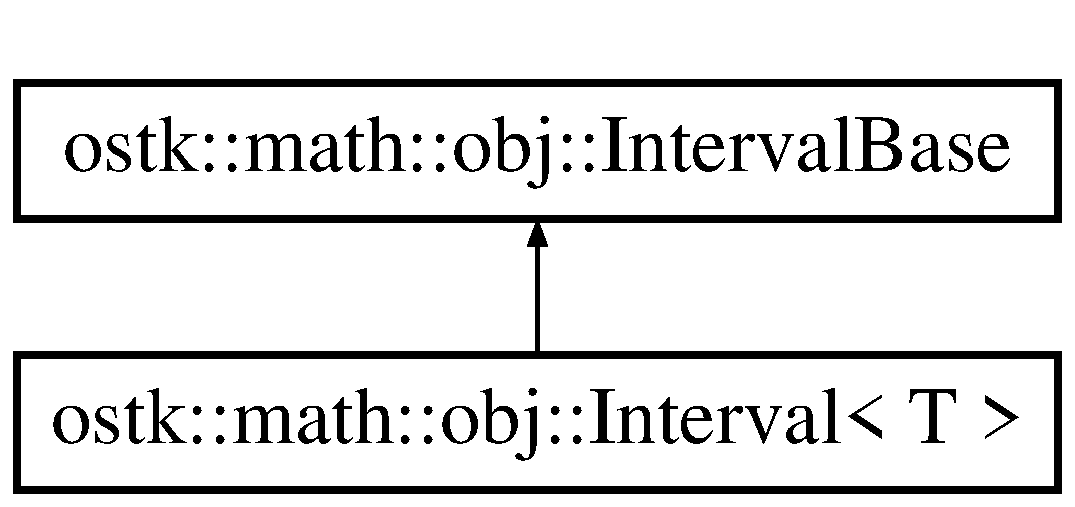
\includegraphics[height=2.000000cm]{classostk_1_1math_1_1obj_1_1_interval_base}
\end{center}
\end{figure}
\doxysubsection*{Public Types}
\begin{DoxyCompactItemize}
\item 
enum \mbox{\hyperlink{classostk_1_1math_1_1obj_1_1_interval_base_a0dd9bd29a9bfefa26de9b88ac81de92a}{Type}} \{ \newline
\mbox{\hyperlink{classostk_1_1math_1_1obj_1_1_interval_base_a0dd9bd29a9bfefa26de9b88ac81de92aaec0fc0100c4fc1ce4eea230c3dc10360}{Type\+::\+Undefined}}, 
\mbox{\hyperlink{classostk_1_1math_1_1obj_1_1_interval_base_a0dd9bd29a9bfefa26de9b88ac81de92aa03f4a47830f97377a35321051685071e}{Type\+::\+Closed}}, 
\mbox{\hyperlink{classostk_1_1math_1_1obj_1_1_interval_base_a0dd9bd29a9bfefa26de9b88ac81de92aac3bf447eabe632720a3aa1a7ce401274}{Type\+::\+Open}}, 
\mbox{\hyperlink{classostk_1_1math_1_1obj_1_1_interval_base_a0dd9bd29a9bfefa26de9b88ac81de92aab5e08f9173f660e791d3ba99ff8281d7}{Type\+::\+Half\+Open\+Left}}, 
\newline
\mbox{\hyperlink{classostk_1_1math_1_1obj_1_1_interval_base_a0dd9bd29a9bfefa26de9b88ac81de92aa484f1b37e0208f622a1e6f7a3ff8c2c3}{Type\+::\+Half\+Open\+Right}}
 \}
\begin{DoxyCompactList}\small\item\em \mbox{\hyperlink{classostk_1_1math_1_1obj_1_1_interval}{Interval}} type. \end{DoxyCompactList}\end{DoxyCompactItemize}


\doxysubsection{Detailed Description}
\mbox{\hyperlink{classostk_1_1math_1_1obj_1_1_interval}{Interval}} base (used to avoid having a templated enum) 

\doxysubsection{Member Enumeration Documentation}
\mbox{\Hypertarget{classostk_1_1math_1_1obj_1_1_interval_base_a0dd9bd29a9bfefa26de9b88ac81de92a}\label{classostk_1_1math_1_1obj_1_1_interval_base_a0dd9bd29a9bfefa26de9b88ac81de92a}} 
\index{ostk::math::obj::IntervalBase@{ostk::math::obj::IntervalBase}!Type@{Type}}
\index{Type@{Type}!ostk::math::obj::IntervalBase@{ostk::math::obj::IntervalBase}}
\doxysubsubsection{\texorpdfstring{Type}{Type}}
{\footnotesize\ttfamily enum \mbox{\hyperlink{classostk_1_1math_1_1obj_1_1_interval_base_a0dd9bd29a9bfefa26de9b88ac81de92a}{ostk\+::math\+::obj\+::\+Interval\+Base\+::\+Type}}\hspace{0.3cm}{\ttfamily [strong]}}



\mbox{\hyperlink{classostk_1_1math_1_1obj_1_1_interval}{Interval}} type. 

\begin{DoxyEnumFields}{Enumerator}
\raisebox{\heightof{T}}[0pt][0pt]{\index{Undefined@{Undefined}!ostk::math::obj::IntervalBase@{ostk::math::obj::IntervalBase}}\index{ostk::math::obj::IntervalBase@{ostk::math::obj::IntervalBase}!Undefined@{Undefined}}}\mbox{\Hypertarget{classostk_1_1math_1_1obj_1_1_interval_base_a0dd9bd29a9bfefa26de9b88ac81de92aaec0fc0100c4fc1ce4eea230c3dc10360}\label{classostk_1_1math_1_1obj_1_1_interval_base_a0dd9bd29a9bfefa26de9b88ac81de92aaec0fc0100c4fc1ce4eea230c3dc10360}} 
Undefined&Undefined interval type. \\
\hline

\raisebox{\heightof{T}}[0pt][0pt]{\index{Closed@{Closed}!ostk::math::obj::IntervalBase@{ostk::math::obj::IntervalBase}}\index{ostk::math::obj::IntervalBase@{ostk::math::obj::IntervalBase}!Closed@{Closed}}}\mbox{\Hypertarget{classostk_1_1math_1_1obj_1_1_interval_base_a0dd9bd29a9bfefa26de9b88ac81de92aa03f4a47830f97377a35321051685071e}\label{classostk_1_1math_1_1obj_1_1_interval_base_a0dd9bd29a9bfefa26de9b88ac81de92aa03f4a47830f97377a35321051685071e}} 
Closed&Closed interval type \mbox{[}a, b\mbox{]}. \\
\hline

\raisebox{\heightof{T}}[0pt][0pt]{\index{Open@{Open}!ostk::math::obj::IntervalBase@{ostk::math::obj::IntervalBase}}\index{ostk::math::obj::IntervalBase@{ostk::math::obj::IntervalBase}!Open@{Open}}}\mbox{\Hypertarget{classostk_1_1math_1_1obj_1_1_interval_base_a0dd9bd29a9bfefa26de9b88ac81de92aac3bf447eabe632720a3aa1a7ce401274}\label{classostk_1_1math_1_1obj_1_1_interval_base_a0dd9bd29a9bfefa26de9b88ac81de92aac3bf447eabe632720a3aa1a7ce401274}} 
Open&Open interval type \mbox{]}a, b\mbox{[}. \\
\hline

\raisebox{\heightof{T}}[0pt][0pt]{\index{HalfOpenLeft@{HalfOpenLeft}!ostk::math::obj::IntervalBase@{ostk::math::obj::IntervalBase}}\index{ostk::math::obj::IntervalBase@{ostk::math::obj::IntervalBase}!HalfOpenLeft@{HalfOpenLeft}}}\mbox{\Hypertarget{classostk_1_1math_1_1obj_1_1_interval_base_a0dd9bd29a9bfefa26de9b88ac81de92aab5e08f9173f660e791d3ba99ff8281d7}\label{classostk_1_1math_1_1obj_1_1_interval_base_a0dd9bd29a9bfefa26de9b88ac81de92aab5e08f9173f660e791d3ba99ff8281d7}} 
Half\+Open\+Left&Half-\/open left interval type \mbox{]}a, b\mbox{]}. \\
\hline

\raisebox{\heightof{T}}[0pt][0pt]{\index{HalfOpenRight@{HalfOpenRight}!ostk::math::obj::IntervalBase@{ostk::math::obj::IntervalBase}}\index{ostk::math::obj::IntervalBase@{ostk::math::obj::IntervalBase}!HalfOpenRight@{HalfOpenRight}}}\mbox{\Hypertarget{classostk_1_1math_1_1obj_1_1_interval_base_a0dd9bd29a9bfefa26de9b88ac81de92aa484f1b37e0208f622a1e6f7a3ff8c2c3}\label{classostk_1_1math_1_1obj_1_1_interval_base_a0dd9bd29a9bfefa26de9b88ac81de92aa484f1b37e0208f622a1e6f7a3ff8c2c3}} 
Half\+Open\+Right&Half-\/open right interval type \mbox{[}a, b\mbox{[}. \\
\hline

\end{DoxyEnumFields}


The documentation for this class was generated from the following file\+:\begin{DoxyCompactItemize}
\item 
include/\+Open\+Space\+Toolkit/\+Mathematics/\+Objects/\mbox{\hyperlink{_interval_8hpp}{Interval.\+hpp}}\end{DoxyCompactItemize}

\hypertarget{classostk_1_1math_1_1geom_1_1d3_1_1objects_1_1_line}{}\doxysection{ostk\+::math\+::geom\+::d3\+::objects\+::Line Class Reference}
\label{classostk_1_1math_1_1geom_1_1d3_1_1objects_1_1_line}\index{ostk::math::geom::d3::objects::Line@{ostk::math::geom::d3::objects::Line}}


\mbox{\hyperlink{classostk_1_1math_1_1geom_1_1d3_1_1objects_1_1_line}{Line}}.  




{\ttfamily \#include $<$Line.\+hpp$>$}

Inheritance diagram for ostk\+::math\+::geom\+::d3\+::objects\+::Line\+:\begin{figure}[H]
\begin{center}
\leavevmode
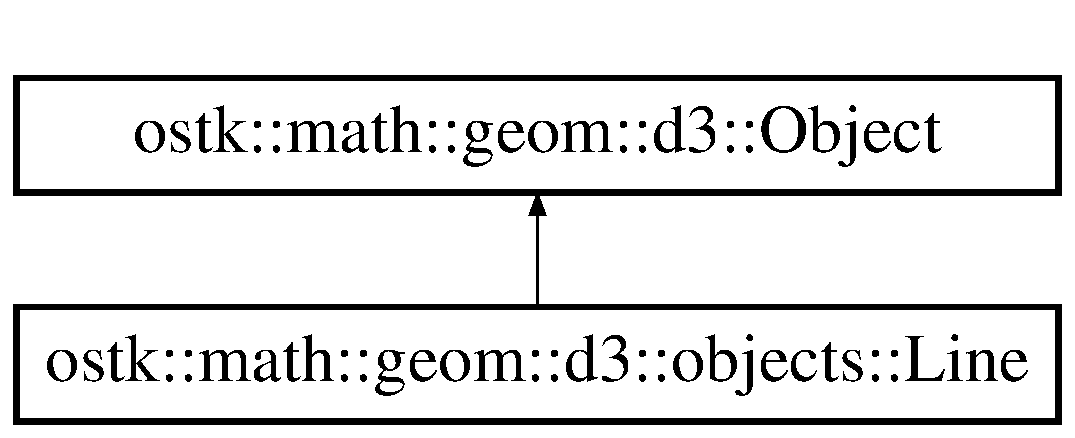
\includegraphics[height=2.000000cm]{classostk_1_1math_1_1geom_1_1d3_1_1objects_1_1_line}
\end{center}
\end{figure}
\doxysubsection*{Public Member Functions}
\begin{DoxyCompactItemize}
\item 
\mbox{\hyperlink{classostk_1_1math_1_1geom_1_1d3_1_1objects_1_1_line_a9ebdaaf67a4bd91780808f8683463ebe}{Line}} (const \mbox{\hyperlink{classostk_1_1math_1_1geom_1_1d3_1_1objects_1_1_point}{Point}} \&an\+Origin, const Vector3d \&a\+Direction)
\begin{DoxyCompactList}\small\item\em Constructor. \end{DoxyCompactList}\item 
virtual \mbox{\hyperlink{classostk_1_1math_1_1geom_1_1d3_1_1objects_1_1_line}{Line}} $\ast$ \mbox{\hyperlink{classostk_1_1math_1_1geom_1_1d3_1_1objects_1_1_line_aaf6fc08cf6b690b88c52d112052ce226}{clone}} () const override
\begin{DoxyCompactList}\small\item\em Clone line. \end{DoxyCompactList}\item 
bool \mbox{\hyperlink{classostk_1_1math_1_1geom_1_1d3_1_1objects_1_1_line_a60d23a12b6f81685f430c0fd8ff07752}{operator==}} (const \mbox{\hyperlink{classostk_1_1math_1_1geom_1_1d3_1_1objects_1_1_line}{Line}} \&a\+Line) const
\begin{DoxyCompactList}\small\item\em Equal to operator. \end{DoxyCompactList}\item 
bool \mbox{\hyperlink{classostk_1_1math_1_1geom_1_1d3_1_1objects_1_1_line_ae2dad60d3d1b08f5d17a2d87839d0830}{operator!=}} (const \mbox{\hyperlink{classostk_1_1math_1_1geom_1_1d3_1_1objects_1_1_line}{Line}} \&a\+Line) const
\begin{DoxyCompactList}\small\item\em Not equal to operator. \end{DoxyCompactList}\item 
virtual bool \mbox{\hyperlink{classostk_1_1math_1_1geom_1_1d3_1_1objects_1_1_line_a092640b8e18d71c734185f326698f518}{is\+Defined}} () const override
\begin{DoxyCompactList}\small\item\em Check if line is defined. \end{DoxyCompactList}\item 
bool \mbox{\hyperlink{classostk_1_1math_1_1geom_1_1d3_1_1objects_1_1_line_a65d3865e67da2d1629fa1e302a2c62fe}{intersects}} (const \mbox{\hyperlink{classostk_1_1math_1_1geom_1_1d3_1_1objects_1_1_point}{Point}} \&a\+Point) const
\begin{DoxyCompactList}\small\item\em Check if line intersects point. \end{DoxyCompactList}\item 
bool \mbox{\hyperlink{classostk_1_1math_1_1geom_1_1d3_1_1objects_1_1_line_a292e86df1d673e4f040691b25877a6ce}{intersects}} (const \mbox{\hyperlink{classostk_1_1math_1_1geom_1_1d3_1_1objects_1_1_plane}{Plane}} \&a\+Plane) const
\begin{DoxyCompactList}\small\item\em Check if line intersects plane. \end{DoxyCompactList}\item 
bool \mbox{\hyperlink{classostk_1_1math_1_1geom_1_1d3_1_1objects_1_1_line_a5300ab7d6cbe87cf74de014252956558}{intersects}} (const \mbox{\hyperlink{classostk_1_1math_1_1geom_1_1d3_1_1objects_1_1_sphere}{Sphere}} \&a\+Sphere) const
\begin{DoxyCompactList}\small\item\em Check if line intersects sphere. \end{DoxyCompactList}\item 
bool \mbox{\hyperlink{classostk_1_1math_1_1geom_1_1d3_1_1objects_1_1_line_a72843cbf3252ed608969e7c4d9a1592f}{intersects}} (const \mbox{\hyperlink{classostk_1_1math_1_1geom_1_1d3_1_1objects_1_1_ellipsoid}{Ellipsoid}} \&an\+Ellipsoid) const
\begin{DoxyCompactList}\small\item\em Check if line intersects ellipsoid. \end{DoxyCompactList}\item 
bool \mbox{\hyperlink{classostk_1_1math_1_1geom_1_1d3_1_1objects_1_1_line_a51121a95b14948a800a36f57aa85e55a}{contains}} (const \mbox{\hyperlink{classostk_1_1math_1_1geom_1_1d3_1_1objects_1_1_point}{Point}} \&a\+Point) const
\begin{DoxyCompactList}\small\item\em Check if line contains point. \end{DoxyCompactList}\item 
bool \mbox{\hyperlink{classostk_1_1math_1_1geom_1_1d3_1_1objects_1_1_line_a63fe1d825e847ba201c50ddf2d02ee1e}{contains}} (const \mbox{\hyperlink{classostk_1_1math_1_1geom_1_1d3_1_1objects_1_1_point_set}{Point\+Set}} \&a\+Point\+Set) const
\begin{DoxyCompactList}\small\item\em Check if line contains point set. \end{DoxyCompactList}\item 
\mbox{\hyperlink{classostk_1_1math_1_1geom_1_1d3_1_1objects_1_1_point}{Point}} \mbox{\hyperlink{classostk_1_1math_1_1geom_1_1d3_1_1objects_1_1_line_afc9e2dbb4641c031b91c4b8019a41b69}{get\+Origin}} () const
\begin{DoxyCompactList}\small\item\em Get line origin. \end{DoxyCompactList}\item 
Vector3d \mbox{\hyperlink{classostk_1_1math_1_1geom_1_1d3_1_1objects_1_1_line_a7f312d93308a5f0a876d69c46662838b}{get\+Direction}} () const
\begin{DoxyCompactList}\small\item\em Get line direction. \end{DoxyCompactList}\item 
Real \mbox{\hyperlink{classostk_1_1math_1_1geom_1_1d3_1_1objects_1_1_line_acbc844b79bd79c92641828baefee8eb7}{distance\+To}} (const \mbox{\hyperlink{classostk_1_1math_1_1geom_1_1d3_1_1objects_1_1_point}{Point}} \&a\+Point) const
\begin{DoxyCompactList}\small\item\em Get distance to point. \end{DoxyCompactList}\item 
\mbox{\hyperlink{classostk_1_1math_1_1geom_1_1d3_1_1_intersection}{Intersection}} \mbox{\hyperlink{classostk_1_1math_1_1geom_1_1d3_1_1objects_1_1_line_a3dba3152c9257eb58f2437c687e410db}{intersection\+With}} (const \mbox{\hyperlink{classostk_1_1math_1_1geom_1_1d3_1_1objects_1_1_plane}{Plane}} \&a\+Plane) const
\begin{DoxyCompactList}\small\item\em Compute intersection of line with plane. \end{DoxyCompactList}\item 
virtual void \mbox{\hyperlink{classostk_1_1math_1_1geom_1_1d3_1_1objects_1_1_line_ad3e7bf31cdde2d265dd9ff644b341f2d}{print}} (std\+::ostream \&an\+Output\+Stream, bool display\+Decorators=true) const override
\begin{DoxyCompactList}\small\item\em Print line. \end{DoxyCompactList}\item 
virtual void \mbox{\hyperlink{classostk_1_1math_1_1geom_1_1d3_1_1objects_1_1_line_ab12eb788b966601d6d09f75196a30d6f}{apply\+Transformation}} (const \mbox{\hyperlink{classostk_1_1math_1_1geom_1_1d3_1_1_transformation}{Transformation}} \&a\+Transformation) override
\begin{DoxyCompactList}\small\item\em Apply transformation to line. \end{DoxyCompactList}\end{DoxyCompactItemize}
\doxysubsection*{Static Public Member Functions}
\begin{DoxyCompactItemize}
\item 
static \mbox{\hyperlink{classostk_1_1math_1_1geom_1_1d3_1_1objects_1_1_line}{Line}} \mbox{\hyperlink{classostk_1_1math_1_1geom_1_1d3_1_1objects_1_1_line_aa22d1d366cfaf4083977a332de24f621}{Undefined}} ()
\begin{DoxyCompactList}\small\item\em Constructs an undefined line. \end{DoxyCompactList}\item 
static \mbox{\hyperlink{classostk_1_1math_1_1geom_1_1d3_1_1objects_1_1_line}{Line}} \mbox{\hyperlink{classostk_1_1math_1_1geom_1_1d3_1_1objects_1_1_line_a23ebcd8b2720d8daefba7191eccdf8cb}{Points}} (const \mbox{\hyperlink{classostk_1_1math_1_1geom_1_1d3_1_1objects_1_1_point}{Point}} \&a\+First\+Point, const \mbox{\hyperlink{classostk_1_1math_1_1geom_1_1d3_1_1objects_1_1_point}{Point}} \&a\+Second\+Point)
\begin{DoxyCompactList}\small\item\em Constructs a line using two points. \end{DoxyCompactList}\end{DoxyCompactItemize}


\doxysubsection{Detailed Description}
\mbox{\hyperlink{classostk_1_1math_1_1geom_1_1d3_1_1objects_1_1_line}{Line}}. 

\href{https://en.wikipedia.org/wiki/Line_}{\texttt{ https\+://en.\+wikipedia.\+org/wiki/\+Line\+\_\+}}(geometry) 

\doxysubsection{Constructor \& Destructor Documentation}
\mbox{\Hypertarget{classostk_1_1math_1_1geom_1_1d3_1_1objects_1_1_line_a9ebdaaf67a4bd91780808f8683463ebe}\label{classostk_1_1math_1_1geom_1_1d3_1_1objects_1_1_line_a9ebdaaf67a4bd91780808f8683463ebe}} 
\index{ostk::math::geom::d3::objects::Line@{ostk::math::geom::d3::objects::Line}!Line@{Line}}
\index{Line@{Line}!ostk::math::geom::d3::objects::Line@{ostk::math::geom::d3::objects::Line}}
\doxysubsubsection{\texorpdfstring{Line()}{Line()}}
{\footnotesize\ttfamily ostk\+::math\+::geom\+::d3\+::objects\+::\+Line\+::\+Line (\begin{DoxyParamCaption}\item[{const \mbox{\hyperlink{classostk_1_1math_1_1geom_1_1d3_1_1objects_1_1_point}{Point}} \&}]{an\+Origin,  }\item[{const Vector3d \&}]{a\+Direction }\end{DoxyParamCaption})}



Constructor. 


\begin{DoxyCode}{0}
\DoxyCodeLine{\mbox{\hyperlink{classostk_1_1math_1_1geom_1_1d3_1_1objects_1_1_line_a9ebdaaf67a4bd91780808f8683463ebe}{Line}} line(\{ 0.0, 0.0, 0.0 \}, \{ 0.0, 0.0, 1.0 \}) ;}
\end{DoxyCode}



\begin{DoxyParams}[1]{Parameters}
\mbox{\texttt{ in}}  & {\em an\+Origin} & A line origin \\
\hline
\mbox{\texttt{ in}}  & {\em a\+Direction} & A line direction \\
\hline
\end{DoxyParams}


\doxysubsection{Member Function Documentation}
\mbox{\Hypertarget{classostk_1_1math_1_1geom_1_1d3_1_1objects_1_1_line_ab12eb788b966601d6d09f75196a30d6f}\label{classostk_1_1math_1_1geom_1_1d3_1_1objects_1_1_line_ab12eb788b966601d6d09f75196a30d6f}} 
\index{ostk::math::geom::d3::objects::Line@{ostk::math::geom::d3::objects::Line}!applyTransformation@{applyTransformation}}
\index{applyTransformation@{applyTransformation}!ostk::math::geom::d3::objects::Line@{ostk::math::geom::d3::objects::Line}}
\doxysubsubsection{\texorpdfstring{applyTransformation()}{applyTransformation()}}
{\footnotesize\ttfamily void ostk\+::math\+::geom\+::d3\+::objects\+::\+Line\+::apply\+Transformation (\begin{DoxyParamCaption}\item[{const \mbox{\hyperlink{classostk_1_1math_1_1geom_1_1d3_1_1_transformation}{Transformation}} \&}]{a\+Transformation }\end{DoxyParamCaption})\hspace{0.3cm}{\ttfamily [override]}, {\ttfamily [virtual]}}



Apply transformation to line. 


\begin{DoxyParams}[1]{Parameters}
\mbox{\texttt{ in}}  & {\em a\+Transformation} & A transformation \\
\hline
\end{DoxyParams}


Implements \mbox{\hyperlink{classostk_1_1math_1_1geom_1_1d3_1_1_object_ae9194dd6d2bb4df09292ffc84dccdb1d}{ostk\+::math\+::geom\+::d3\+::\+Object}}.

\mbox{\Hypertarget{classostk_1_1math_1_1geom_1_1d3_1_1objects_1_1_line_aaf6fc08cf6b690b88c52d112052ce226}\label{classostk_1_1math_1_1geom_1_1d3_1_1objects_1_1_line_aaf6fc08cf6b690b88c52d112052ce226}} 
\index{ostk::math::geom::d3::objects::Line@{ostk::math::geom::d3::objects::Line}!clone@{clone}}
\index{clone@{clone}!ostk::math::geom::d3::objects::Line@{ostk::math::geom::d3::objects::Line}}
\doxysubsubsection{\texorpdfstring{clone()}{clone()}}
{\footnotesize\ttfamily \mbox{\hyperlink{classostk_1_1math_1_1geom_1_1d3_1_1objects_1_1_line}{Line}} $\ast$ ostk\+::math\+::geom\+::d3\+::objects\+::\+Line\+::clone (\begin{DoxyParamCaption}{ }\end{DoxyParamCaption}) const\hspace{0.3cm}{\ttfamily [override]}, {\ttfamily [virtual]}}



Clone line. 

\begin{DoxyReturn}{Returns}
Pointer to cloned line 
\end{DoxyReturn}


Implements \mbox{\hyperlink{classostk_1_1math_1_1geom_1_1d3_1_1_object_a676013f9555f6492687f9809b2db887b}{ostk\+::math\+::geom\+::d3\+::\+Object}}.

\mbox{\Hypertarget{classostk_1_1math_1_1geom_1_1d3_1_1objects_1_1_line_a51121a95b14948a800a36f57aa85e55a}\label{classostk_1_1math_1_1geom_1_1d3_1_1objects_1_1_line_a51121a95b14948a800a36f57aa85e55a}} 
\index{ostk::math::geom::d3::objects::Line@{ostk::math::geom::d3::objects::Line}!contains@{contains}}
\index{contains@{contains}!ostk::math::geom::d3::objects::Line@{ostk::math::geom::d3::objects::Line}}
\doxysubsubsection{\texorpdfstring{contains()}{contains()}\hspace{0.1cm}{\footnotesize\ttfamily [1/2]}}
{\footnotesize\ttfamily bool ostk\+::math\+::geom\+::d3\+::objects\+::\+Line\+::contains (\begin{DoxyParamCaption}\item[{const \mbox{\hyperlink{classostk_1_1math_1_1geom_1_1d3_1_1objects_1_1_point}{Point}} \&}]{a\+Point }\end{DoxyParamCaption}) const}



Check if line contains point. 


\begin{DoxyCode}{0}
\DoxyCodeLine{\mbox{\hyperlink{classostk_1_1math_1_1geom_1_1d3_1_1objects_1_1_line_a9ebdaaf67a4bd91780808f8683463ebe}{Line}} line = ... ;}
\DoxyCodeLine{Point point = ... ;}
\DoxyCodeLine{line.contains(point) ;}
\end{DoxyCode}



\begin{DoxyParams}[1]{Parameters}
\mbox{\texttt{ in}}  & {\em a\+Point} & A point \\
\hline
\end{DoxyParams}
\begin{DoxyReturn}{Returns}
True if line contains point 
\end{DoxyReturn}
\mbox{\Hypertarget{classostk_1_1math_1_1geom_1_1d3_1_1objects_1_1_line_a63fe1d825e847ba201c50ddf2d02ee1e}\label{classostk_1_1math_1_1geom_1_1d3_1_1objects_1_1_line_a63fe1d825e847ba201c50ddf2d02ee1e}} 
\index{ostk::math::geom::d3::objects::Line@{ostk::math::geom::d3::objects::Line}!contains@{contains}}
\index{contains@{contains}!ostk::math::geom::d3::objects::Line@{ostk::math::geom::d3::objects::Line}}
\doxysubsubsection{\texorpdfstring{contains()}{contains()}\hspace{0.1cm}{\footnotesize\ttfamily [2/2]}}
{\footnotesize\ttfamily bool ostk\+::math\+::geom\+::d3\+::objects\+::\+Line\+::contains (\begin{DoxyParamCaption}\item[{const \mbox{\hyperlink{classostk_1_1math_1_1geom_1_1d3_1_1objects_1_1_point_set}{Point\+Set}} \&}]{a\+Point\+Set }\end{DoxyParamCaption}) const}



Check if line contains point set. 


\begin{DoxyCode}{0}
\DoxyCodeLine{\mbox{\hyperlink{classostk_1_1math_1_1geom_1_1d3_1_1objects_1_1_line_a9ebdaaf67a4bd91780808f8683463ebe}{Line}} line = ... ;}
\DoxyCodeLine{PointSet pointSet = ... ;}
\DoxyCodeLine{line.contains(pointSet) ;}
\end{DoxyCode}



\begin{DoxyParams}[1]{Parameters}
\mbox{\texttt{ in}}  & {\em a\+Point\+Set} & A point set \\
\hline
\end{DoxyParams}
\begin{DoxyReturn}{Returns}
True if line contains point set 
\end{DoxyReturn}
\mbox{\Hypertarget{classostk_1_1math_1_1geom_1_1d3_1_1objects_1_1_line_acbc844b79bd79c92641828baefee8eb7}\label{classostk_1_1math_1_1geom_1_1d3_1_1objects_1_1_line_acbc844b79bd79c92641828baefee8eb7}} 
\index{ostk::math::geom::d3::objects::Line@{ostk::math::geom::d3::objects::Line}!distanceTo@{distanceTo}}
\index{distanceTo@{distanceTo}!ostk::math::geom::d3::objects::Line@{ostk::math::geom::d3::objects::Line}}
\doxysubsubsection{\texorpdfstring{distanceTo()}{distanceTo()}}
{\footnotesize\ttfamily Real ostk\+::math\+::geom\+::d3\+::objects\+::\+Line\+::distance\+To (\begin{DoxyParamCaption}\item[{const \mbox{\hyperlink{classostk_1_1math_1_1geom_1_1d3_1_1objects_1_1_point}{Point}} \&}]{a\+Point }\end{DoxyParamCaption}) const}



Get distance to point. 


\begin{DoxyParams}[1]{Parameters}
\mbox{\texttt{ in}}  & {\em a\+Point} & A point \\
\hline
\end{DoxyParams}
\begin{DoxyReturn}{Returns}
Distance to point 
\end{DoxyReturn}
\mbox{\Hypertarget{classostk_1_1math_1_1geom_1_1d3_1_1objects_1_1_line_a7f312d93308a5f0a876d69c46662838b}\label{classostk_1_1math_1_1geom_1_1d3_1_1objects_1_1_line_a7f312d93308a5f0a876d69c46662838b}} 
\index{ostk::math::geom::d3::objects::Line@{ostk::math::geom::d3::objects::Line}!getDirection@{getDirection}}
\index{getDirection@{getDirection}!ostk::math::geom::d3::objects::Line@{ostk::math::geom::d3::objects::Line}}
\doxysubsubsection{\texorpdfstring{getDirection()}{getDirection()}}
{\footnotesize\ttfamily Vector3d ostk\+::math\+::geom\+::d3\+::objects\+::\+Line\+::get\+Direction (\begin{DoxyParamCaption}{ }\end{DoxyParamCaption}) const}



Get line direction. 


\begin{DoxyCode}{0}
\DoxyCodeLine{\mbox{\hyperlink{classostk_1_1math_1_1geom_1_1d3_1_1objects_1_1_line_a9ebdaaf67a4bd91780808f8683463ebe}{Line}}(\{ 0.0, 0.0, 0.0 \}, \{ 0.0, 0.0, 1.0 \}).\mbox{\hyperlink{classostk_1_1math_1_1geom_1_1d3_1_1objects_1_1_line_a7f312d93308a5f0a876d69c46662838b}{getDirection}}() ; \textcolor{comment}{// [0.0, 0.0, 1.0]}}
\end{DoxyCode}


\begin{DoxyReturn}{Returns}
\mbox{\hyperlink{classostk_1_1math_1_1geom_1_1d3_1_1objects_1_1_line}{Line}} direction 
\end{DoxyReturn}
\mbox{\Hypertarget{classostk_1_1math_1_1geom_1_1d3_1_1objects_1_1_line_afc9e2dbb4641c031b91c4b8019a41b69}\label{classostk_1_1math_1_1geom_1_1d3_1_1objects_1_1_line_afc9e2dbb4641c031b91c4b8019a41b69}} 
\index{ostk::math::geom::d3::objects::Line@{ostk::math::geom::d3::objects::Line}!getOrigin@{getOrigin}}
\index{getOrigin@{getOrigin}!ostk::math::geom::d3::objects::Line@{ostk::math::geom::d3::objects::Line}}
\doxysubsubsection{\texorpdfstring{getOrigin()}{getOrigin()}}
{\footnotesize\ttfamily \mbox{\hyperlink{classostk_1_1math_1_1geom_1_1d3_1_1objects_1_1_point}{Point}} ostk\+::math\+::geom\+::d3\+::objects\+::\+Line\+::get\+Origin (\begin{DoxyParamCaption}{ }\end{DoxyParamCaption}) const}



Get line origin. 


\begin{DoxyCode}{0}
\DoxyCodeLine{\mbox{\hyperlink{classostk_1_1math_1_1geom_1_1d3_1_1objects_1_1_line_a9ebdaaf67a4bd91780808f8683463ebe}{Line}}(\{ 0.0, 0.0, 0.0 \}, \{ 0.0, 0.0, 1.0 \}).\mbox{\hyperlink{classostk_1_1math_1_1geom_1_1d3_1_1objects_1_1_line_afc9e2dbb4641c031b91c4b8019a41b69}{getOrigin}}() ; \textcolor{comment}{// [0.0, 0.0, 0.0]}}
\end{DoxyCode}


\begin{DoxyReturn}{Returns}
\mbox{\hyperlink{classostk_1_1math_1_1geom_1_1d3_1_1objects_1_1_line}{Line}} origin 
\end{DoxyReturn}
\mbox{\Hypertarget{classostk_1_1math_1_1geom_1_1d3_1_1objects_1_1_line_a3dba3152c9257eb58f2437c687e410db}\label{classostk_1_1math_1_1geom_1_1d3_1_1objects_1_1_line_a3dba3152c9257eb58f2437c687e410db}} 
\index{ostk::math::geom::d3::objects::Line@{ostk::math::geom::d3::objects::Line}!intersectionWith@{intersectionWith}}
\index{intersectionWith@{intersectionWith}!ostk::math::geom::d3::objects::Line@{ostk::math::geom::d3::objects::Line}}
\doxysubsubsection{\texorpdfstring{intersectionWith()}{intersectionWith()}}
{\footnotesize\ttfamily \mbox{\hyperlink{classostk_1_1math_1_1geom_1_1d3_1_1_intersection}{Intersection}} ostk\+::math\+::geom\+::d3\+::objects\+::\+Line\+::intersection\+With (\begin{DoxyParamCaption}\item[{const \mbox{\hyperlink{classostk_1_1math_1_1geom_1_1d3_1_1objects_1_1_plane}{Plane}} \&}]{a\+Plane }\end{DoxyParamCaption}) const}



Compute intersection of line with plane. 


\begin{DoxyParams}[1]{Parameters}
\mbox{\texttt{ in}}  & {\em a\+Plane} & A plane \\
\hline
\end{DoxyParams}
\begin{DoxyReturn}{Returns}
\mbox{\hyperlink{classostk_1_1math_1_1geom_1_1d3_1_1_intersection}{Intersection}} of line with plane 
\end{DoxyReturn}
\mbox{\Hypertarget{classostk_1_1math_1_1geom_1_1d3_1_1objects_1_1_line_a72843cbf3252ed608969e7c4d9a1592f}\label{classostk_1_1math_1_1geom_1_1d3_1_1objects_1_1_line_a72843cbf3252ed608969e7c4d9a1592f}} 
\index{ostk::math::geom::d3::objects::Line@{ostk::math::geom::d3::objects::Line}!intersects@{intersects}}
\index{intersects@{intersects}!ostk::math::geom::d3::objects::Line@{ostk::math::geom::d3::objects::Line}}
\doxysubsubsection{\texorpdfstring{intersects()}{intersects()}\hspace{0.1cm}{\footnotesize\ttfamily [1/4]}}
{\footnotesize\ttfamily bool ostk\+::math\+::geom\+::d3\+::objects\+::\+Line\+::intersects (\begin{DoxyParamCaption}\item[{const \mbox{\hyperlink{classostk_1_1math_1_1geom_1_1d3_1_1objects_1_1_ellipsoid}{Ellipsoid}} \&}]{an\+Ellipsoid }\end{DoxyParamCaption}) const}



Check if line intersects ellipsoid. 


\begin{DoxyCode}{0}
\DoxyCodeLine{\mbox{\hyperlink{classostk_1_1math_1_1geom_1_1d3_1_1objects_1_1_line_a9ebdaaf67a4bd91780808f8683463ebe}{Line}} line = ... ;}
\DoxyCodeLine{Ellipsoid ellipsoid = ... ;}
\DoxyCodeLine{line.intersects(ellipsoid) ;}
\end{DoxyCode}



\begin{DoxyParams}[1]{Parameters}
\mbox{\texttt{ in}}  & {\em an\+Ellipsoid} & An ellipsoid \\
\hline
\end{DoxyParams}
\begin{DoxyReturn}{Returns}
True if line intersects ellipsoid 
\end{DoxyReturn}
\mbox{\Hypertarget{classostk_1_1math_1_1geom_1_1d3_1_1objects_1_1_line_a292e86df1d673e4f040691b25877a6ce}\label{classostk_1_1math_1_1geom_1_1d3_1_1objects_1_1_line_a292e86df1d673e4f040691b25877a6ce}} 
\index{ostk::math::geom::d3::objects::Line@{ostk::math::geom::d3::objects::Line}!intersects@{intersects}}
\index{intersects@{intersects}!ostk::math::geom::d3::objects::Line@{ostk::math::geom::d3::objects::Line}}
\doxysubsubsection{\texorpdfstring{intersects()}{intersects()}\hspace{0.1cm}{\footnotesize\ttfamily [2/4]}}
{\footnotesize\ttfamily bool ostk\+::math\+::geom\+::d3\+::objects\+::\+Line\+::intersects (\begin{DoxyParamCaption}\item[{const \mbox{\hyperlink{classostk_1_1math_1_1geom_1_1d3_1_1objects_1_1_plane}{Plane}} \&}]{a\+Plane }\end{DoxyParamCaption}) const}



Check if line intersects plane. 


\begin{DoxyCode}{0}
\DoxyCodeLine{\mbox{\hyperlink{classostk_1_1math_1_1geom_1_1d3_1_1objects_1_1_line_a9ebdaaf67a4bd91780808f8683463ebe}{Line}} line = ... ;}
\DoxyCodeLine{Plane plane = ... ;}
\DoxyCodeLine{line.intersects(plane) ;}
\end{DoxyCode}



\begin{DoxyParams}[1]{Parameters}
\mbox{\texttt{ in}}  & {\em a\+Plane} & A plane \\
\hline
\end{DoxyParams}
\begin{DoxyReturn}{Returns}
True if line intersects plane 
\end{DoxyReturn}
\mbox{\Hypertarget{classostk_1_1math_1_1geom_1_1d3_1_1objects_1_1_line_a65d3865e67da2d1629fa1e302a2c62fe}\label{classostk_1_1math_1_1geom_1_1d3_1_1objects_1_1_line_a65d3865e67da2d1629fa1e302a2c62fe}} 
\index{ostk::math::geom::d3::objects::Line@{ostk::math::geom::d3::objects::Line}!intersects@{intersects}}
\index{intersects@{intersects}!ostk::math::geom::d3::objects::Line@{ostk::math::geom::d3::objects::Line}}
\doxysubsubsection{\texorpdfstring{intersects()}{intersects()}\hspace{0.1cm}{\footnotesize\ttfamily [3/4]}}
{\footnotesize\ttfamily bool ostk\+::math\+::geom\+::d3\+::objects\+::\+Line\+::intersects (\begin{DoxyParamCaption}\item[{const \mbox{\hyperlink{classostk_1_1math_1_1geom_1_1d3_1_1objects_1_1_point}{Point}} \&}]{a\+Point }\end{DoxyParamCaption}) const}



Check if line intersects point. 


\begin{DoxyCode}{0}
\DoxyCodeLine{\mbox{\hyperlink{classostk_1_1math_1_1geom_1_1d3_1_1objects_1_1_line_a9ebdaaf67a4bd91780808f8683463ebe}{Line}} line = ... ;}
\DoxyCodeLine{Point point = ... ;}
\DoxyCodeLine{line.intersects(point) ;}
\end{DoxyCode}



\begin{DoxyParams}[1]{Parameters}
\mbox{\texttt{ in}}  & {\em an\+Point} & A point \\
\hline
\end{DoxyParams}
\begin{DoxyReturn}{Returns}
True if line intersects point 
\end{DoxyReturn}
\mbox{\Hypertarget{classostk_1_1math_1_1geom_1_1d3_1_1objects_1_1_line_a5300ab7d6cbe87cf74de014252956558}\label{classostk_1_1math_1_1geom_1_1d3_1_1objects_1_1_line_a5300ab7d6cbe87cf74de014252956558}} 
\index{ostk::math::geom::d3::objects::Line@{ostk::math::geom::d3::objects::Line}!intersects@{intersects}}
\index{intersects@{intersects}!ostk::math::geom::d3::objects::Line@{ostk::math::geom::d3::objects::Line}}
\doxysubsubsection{\texorpdfstring{intersects()}{intersects()}\hspace{0.1cm}{\footnotesize\ttfamily [4/4]}}
{\footnotesize\ttfamily bool ostk\+::math\+::geom\+::d3\+::objects\+::\+Line\+::intersects (\begin{DoxyParamCaption}\item[{const \mbox{\hyperlink{classostk_1_1math_1_1geom_1_1d3_1_1objects_1_1_sphere}{Sphere}} \&}]{a\+Sphere }\end{DoxyParamCaption}) const}



Check if line intersects sphere. 


\begin{DoxyCode}{0}
\DoxyCodeLine{\mbox{\hyperlink{classostk_1_1math_1_1geom_1_1d3_1_1objects_1_1_line_a9ebdaaf67a4bd91780808f8683463ebe}{Line}} line = ... ;}
\DoxyCodeLine{Sphere sphere = ... ;}
\DoxyCodeLine{line.intersects(sphere) ;}
\end{DoxyCode}



\begin{DoxyParams}[1]{Parameters}
\mbox{\texttt{ in}}  & {\em a\+Sphere} & A sphere \\
\hline
\end{DoxyParams}
\begin{DoxyReturn}{Returns}
True if line intersects sphere 
\end{DoxyReturn}
\mbox{\Hypertarget{classostk_1_1math_1_1geom_1_1d3_1_1objects_1_1_line_a092640b8e18d71c734185f326698f518}\label{classostk_1_1math_1_1geom_1_1d3_1_1objects_1_1_line_a092640b8e18d71c734185f326698f518}} 
\index{ostk::math::geom::d3::objects::Line@{ostk::math::geom::d3::objects::Line}!isDefined@{isDefined}}
\index{isDefined@{isDefined}!ostk::math::geom::d3::objects::Line@{ostk::math::geom::d3::objects::Line}}
\doxysubsubsection{\texorpdfstring{isDefined()}{isDefined()}}
{\footnotesize\ttfamily bool ostk\+::math\+::geom\+::d3\+::objects\+::\+Line\+::is\+Defined (\begin{DoxyParamCaption}{ }\end{DoxyParamCaption}) const\hspace{0.3cm}{\ttfamily [override]}, {\ttfamily [virtual]}}



Check if line is defined. 


\begin{DoxyCode}{0}
\DoxyCodeLine{\mbox{\hyperlink{classostk_1_1math_1_1geom_1_1d3_1_1objects_1_1_line_a9ebdaaf67a4bd91780808f8683463ebe}{Line}}(\{ 0.0, 0.0, 0.0 \}, \{ 0.0, 0.0, 1.0 \}).\mbox{\hyperlink{classostk_1_1math_1_1geom_1_1d3_1_1objects_1_1_line_a092640b8e18d71c734185f326698f518}{isDefined}}() ; \textcolor{comment}{// True}}
\end{DoxyCode}


\begin{DoxyReturn}{Returns}
True if line is defined 
\end{DoxyReturn}


Implements \mbox{\hyperlink{classostk_1_1math_1_1geom_1_1d3_1_1_object_a271a1964cd208be85ce9a0a429395ad8}{ostk\+::math\+::geom\+::d3\+::\+Object}}.

\mbox{\Hypertarget{classostk_1_1math_1_1geom_1_1d3_1_1objects_1_1_line_ae2dad60d3d1b08f5d17a2d87839d0830}\label{classostk_1_1math_1_1geom_1_1d3_1_1objects_1_1_line_ae2dad60d3d1b08f5d17a2d87839d0830}} 
\index{ostk::math::geom::d3::objects::Line@{ostk::math::geom::d3::objects::Line}!operator"!=@{operator"!=}}
\index{operator"!=@{operator"!=}!ostk::math::geom::d3::objects::Line@{ostk::math::geom::d3::objects::Line}}
\doxysubsubsection{\texorpdfstring{operator"!=()}{operator!=()}}
{\footnotesize\ttfamily bool ostk\+::math\+::geom\+::d3\+::objects\+::\+Line\+::operator!= (\begin{DoxyParamCaption}\item[{const \mbox{\hyperlink{classostk_1_1math_1_1geom_1_1d3_1_1objects_1_1_line}{Line}} \&}]{a\+Line }\end{DoxyParamCaption}) const}



Not equal to operator. 


\begin{DoxyCode}{0}
\DoxyCodeLine{\mbox{\hyperlink{classostk_1_1math_1_1geom_1_1d3_1_1objects_1_1_line_a9ebdaaf67a4bd91780808f8683463ebe}{Line}}(\{ 0.0, 0.0, 0.0 \}, \{ 0.0, 0.0, 1.0 \}) != \mbox{\hyperlink{classostk_1_1math_1_1geom_1_1d3_1_1objects_1_1_line_a9ebdaaf67a4bd91780808f8683463ebe}{Line}}(\{ 0.0, 0.0, 0.0 \}, \{ 0.0, 0.0, 2.0 \}) ; \textcolor{comment}{// True}}
\end{DoxyCode}



\begin{DoxyParams}[1]{Parameters}
\mbox{\texttt{ in}}  & {\em a\+Line} & A line \\
\hline
\end{DoxyParams}
\begin{DoxyReturn}{Returns}
True if lines are not equal 
\end{DoxyReturn}
\mbox{\Hypertarget{classostk_1_1math_1_1geom_1_1d3_1_1objects_1_1_line_a60d23a12b6f81685f430c0fd8ff07752}\label{classostk_1_1math_1_1geom_1_1d3_1_1objects_1_1_line_a60d23a12b6f81685f430c0fd8ff07752}} 
\index{ostk::math::geom::d3::objects::Line@{ostk::math::geom::d3::objects::Line}!operator==@{operator==}}
\index{operator==@{operator==}!ostk::math::geom::d3::objects::Line@{ostk::math::geom::d3::objects::Line}}
\doxysubsubsection{\texorpdfstring{operator==()}{operator==()}}
{\footnotesize\ttfamily bool ostk\+::math\+::geom\+::d3\+::objects\+::\+Line\+::operator== (\begin{DoxyParamCaption}\item[{const \mbox{\hyperlink{classostk_1_1math_1_1geom_1_1d3_1_1objects_1_1_line}{Line}} \&}]{a\+Line }\end{DoxyParamCaption}) const}



Equal to operator. 


\begin{DoxyCode}{0}
\DoxyCodeLine{\mbox{\hyperlink{classostk_1_1math_1_1geom_1_1d3_1_1objects_1_1_line_a9ebdaaf67a4bd91780808f8683463ebe}{Line}}(\{ 0.0, 0.0, 0.0 \}, \{ 0.0, 0.0, 1.0 \}) == \mbox{\hyperlink{classostk_1_1math_1_1geom_1_1d3_1_1objects_1_1_line_a9ebdaaf67a4bd91780808f8683463ebe}{Line}}(\{ 0.0, 0.0, 0.0 \}, \{ 0.0, 0.0, 1.0 \}) ; \textcolor{comment}{// True}}
\end{DoxyCode}



\begin{DoxyParams}[1]{Parameters}
\mbox{\texttt{ in}}  & {\em a\+Line} & A line \\
\hline
\end{DoxyParams}
\begin{DoxyReturn}{Returns}
True if lines are equal 
\end{DoxyReturn}
\mbox{\Hypertarget{classostk_1_1math_1_1geom_1_1d3_1_1objects_1_1_line_a23ebcd8b2720d8daefba7191eccdf8cb}\label{classostk_1_1math_1_1geom_1_1d3_1_1objects_1_1_line_a23ebcd8b2720d8daefba7191eccdf8cb}} 
\index{ostk::math::geom::d3::objects::Line@{ostk::math::geom::d3::objects::Line}!Points@{Points}}
\index{Points@{Points}!ostk::math::geom::d3::objects::Line@{ostk::math::geom::d3::objects::Line}}
\doxysubsubsection{\texorpdfstring{Points()}{Points()}}
{\footnotesize\ttfamily \mbox{\hyperlink{classostk_1_1math_1_1geom_1_1d3_1_1objects_1_1_line}{Line}} ostk\+::math\+::geom\+::d3\+::objects\+::\+Line\+::\+Points (\begin{DoxyParamCaption}\item[{const \mbox{\hyperlink{classostk_1_1math_1_1geom_1_1d3_1_1objects_1_1_point}{Point}} \&}]{a\+First\+Point,  }\item[{const \mbox{\hyperlink{classostk_1_1math_1_1geom_1_1d3_1_1objects_1_1_point}{Point}} \&}]{a\+Second\+Point }\end{DoxyParamCaption})\hspace{0.3cm}{\ttfamily [static]}}



Constructs a line using two points. 


\begin{DoxyCode}{0}
\DoxyCodeLine{Point p\_1 = ...}
\DoxyCodeLine{Point p\_2 = ...}
\DoxyCodeLine{Line line = \mbox{\hyperlink{classostk_1_1math_1_1geom_1_1d3_1_1objects_1_1_line_a23ebcd8b2720d8daefba7191eccdf8cb}{Line::Points}}(p\_1, p\_2) ;}
\end{DoxyCode}


\begin{DoxyReturn}{Returns}
\mbox{\hyperlink{classostk_1_1math_1_1geom_1_1d3_1_1objects_1_1_line}{Line}} 
\end{DoxyReturn}
\mbox{\Hypertarget{classostk_1_1math_1_1geom_1_1d3_1_1objects_1_1_line_ad3e7bf31cdde2d265dd9ff644b341f2d}\label{classostk_1_1math_1_1geom_1_1d3_1_1objects_1_1_line_ad3e7bf31cdde2d265dd9ff644b341f2d}} 
\index{ostk::math::geom::d3::objects::Line@{ostk::math::geom::d3::objects::Line}!print@{print}}
\index{print@{print}!ostk::math::geom::d3::objects::Line@{ostk::math::geom::d3::objects::Line}}
\doxysubsubsection{\texorpdfstring{print()}{print()}}
{\footnotesize\ttfamily void ostk\+::math\+::geom\+::d3\+::objects\+::\+Line\+::print (\begin{DoxyParamCaption}\item[{std\+::ostream \&}]{an\+Output\+Stream,  }\item[{bool}]{display\+Decorators = {\ttfamily true} }\end{DoxyParamCaption}) const\hspace{0.3cm}{\ttfamily [override]}, {\ttfamily [virtual]}}



Print line. 


\begin{DoxyParams}[1]{Parameters}
\mbox{\texttt{ in}}  & {\em an\+Output\+Stream} & An output stream \\
\hline
\mbox{\texttt{ in}}  & {\em (optional)} & display\+Decorators If true, display decorators \\
\hline
\end{DoxyParams}


Implements \mbox{\hyperlink{classostk_1_1math_1_1geom_1_1d3_1_1_object_ab2a2a782503b97d1cecabdfedc636fce}{ostk\+::math\+::geom\+::d3\+::\+Object}}.

\mbox{\Hypertarget{classostk_1_1math_1_1geom_1_1d3_1_1objects_1_1_line_aa22d1d366cfaf4083977a332de24f621}\label{classostk_1_1math_1_1geom_1_1d3_1_1objects_1_1_line_aa22d1d366cfaf4083977a332de24f621}} 
\index{ostk::math::geom::d3::objects::Line@{ostk::math::geom::d3::objects::Line}!Undefined@{Undefined}}
\index{Undefined@{Undefined}!ostk::math::geom::d3::objects::Line@{ostk::math::geom::d3::objects::Line}}
\doxysubsubsection{\texorpdfstring{Undefined()}{Undefined()}}
{\footnotesize\ttfamily \mbox{\hyperlink{classostk_1_1math_1_1geom_1_1d3_1_1objects_1_1_line}{Line}} ostk\+::math\+::geom\+::d3\+::objects\+::\+Line\+::\+Undefined (\begin{DoxyParamCaption}{ }\end{DoxyParamCaption})\hspace{0.3cm}{\ttfamily [static]}}



Constructs an undefined line. 


\begin{DoxyCode}{0}
\DoxyCodeLine{\mbox{\hyperlink{classostk_1_1math_1_1geom_1_1d3_1_1objects_1_1_line_a9ebdaaf67a4bd91780808f8683463ebe}{Line}} line = \mbox{\hyperlink{classostk_1_1math_1_1geom_1_1d3_1_1objects_1_1_line_aa22d1d366cfaf4083977a332de24f621}{Line::Undefined}}() ; \textcolor{comment}{// Undefined}}
\end{DoxyCode}


\begin{DoxyReturn}{Returns}
Undefined line 
\end{DoxyReturn}


The documentation for this class was generated from the following files\+:\begin{DoxyCompactItemize}
\item 
include/\+Open\+Space\+Toolkit/\+Mathematics/\+Geometry/3\+D/\+Objects/\mbox{\hyperlink{3_d_2_objects_2_line_8hpp}{Line.\+hpp}}\item 
src/\+Open\+Space\+Toolkit/\+Mathematics/\+Geometry/3\+D/\+Objects/\mbox{\hyperlink{3_d_2_objects_2_line_8cpp}{Line.\+cpp}}\end{DoxyCompactItemize}

\hypertarget{classostk_1_1math_1_1geom_1_1d3_1_1objects_1_1_line_string}{}\doxysection{ostk\+::math\+::geom\+::d3\+::objects\+::Line\+String Class Reference}
\label{classostk_1_1math_1_1geom_1_1d3_1_1objects_1_1_line_string}\index{ostk::math::geom::d3::objects::LineString@{ostk::math::geom::d3::objects::LineString}}


\mbox{\hyperlink{classostk_1_1math_1_1geom_1_1d3_1_1objects_1_1_line}{Line}} string.  




{\ttfamily \#include $<$Line\+String.\+hpp$>$}

Inheritance diagram for ostk\+::math\+::geom\+::d3\+::objects\+::Line\+String\+:\begin{figure}[H]
\begin{center}
\leavevmode
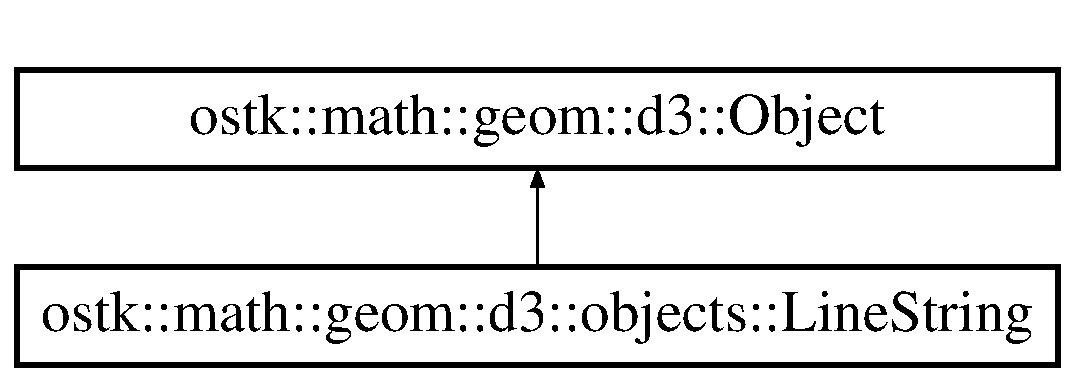
\includegraphics[height=2.000000cm]{classostk_1_1math_1_1geom_1_1d3_1_1objects_1_1_line_string}
\end{center}
\end{figure}
\doxysubsection*{Public Types}
\begin{DoxyCompactItemize}
\item 
typedef Array$<$ \mbox{\hyperlink{classostk_1_1math_1_1geom_1_1d3_1_1objects_1_1_point}{Point}} $>$\+::\mbox{\hyperlink{classostk_1_1math_1_1geom_1_1d3_1_1objects_1_1_line_string_a5d184ce7a4ef5613a621f9b628e56de8}{Const\+Iterator}} \mbox{\hyperlink{classostk_1_1math_1_1geom_1_1d3_1_1objects_1_1_line_string_a5d184ce7a4ef5613a621f9b628e56de8}{Const\+Iterator}}
\end{DoxyCompactItemize}
\doxysubsection*{Public Member Functions}
\begin{DoxyCompactItemize}
\item 
\mbox{\hyperlink{classostk_1_1math_1_1geom_1_1d3_1_1objects_1_1_line_string_a711ebaa7353366ba729bf1ed648fd5a4}{Line\+String}} (const Array$<$ \mbox{\hyperlink{classostk_1_1math_1_1geom_1_1d3_1_1objects_1_1_point}{Point}} $>$ \&a\+Point\+Array)
\begin{DoxyCompactList}\small\item\em Constructor. \end{DoxyCompactList}\item 
virtual \mbox{\hyperlink{classostk_1_1math_1_1geom_1_1d3_1_1objects_1_1_line_string}{Line\+String}} $\ast$ \mbox{\hyperlink{classostk_1_1math_1_1geom_1_1d3_1_1objects_1_1_line_string_acc60289c51f32f822d7ecee85e876a75}{clone}} () const override
\begin{DoxyCompactList}\small\item\em Clone line string. \end{DoxyCompactList}\item 
bool \mbox{\hyperlink{classostk_1_1math_1_1geom_1_1d3_1_1objects_1_1_line_string_a5f01a20d69e144debf566d7244a24d07}{operator==}} (const \mbox{\hyperlink{classostk_1_1math_1_1geom_1_1d3_1_1objects_1_1_line_string}{Line\+String}} \&a\+Line\+String) const
\begin{DoxyCompactList}\small\item\em Equal to operator. \end{DoxyCompactList}\item 
bool \mbox{\hyperlink{classostk_1_1math_1_1geom_1_1d3_1_1objects_1_1_line_string_a7bfdf07c60f6bfd6d4318535696d0eee}{operator!=}} (const \mbox{\hyperlink{classostk_1_1math_1_1geom_1_1d3_1_1objects_1_1_line_string}{Line\+String}} \&a\+Line\+String) const
\begin{DoxyCompactList}\small\item\em Not equal to operator. \end{DoxyCompactList}\item 
virtual bool \mbox{\hyperlink{classostk_1_1math_1_1geom_1_1d3_1_1objects_1_1_line_string_ae55eef3b33fb79290976d5e763ce5190}{is\+Defined}} () const override
\begin{DoxyCompactList}\small\item\em Check if line string is defined. \end{DoxyCompactList}\item 
bool \mbox{\hyperlink{classostk_1_1math_1_1geom_1_1d3_1_1objects_1_1_line_string_a9d80b820c5d81d7f68c831c593f665a1}{is\+Empty}} () const
\begin{DoxyCompactList}\small\item\em Check if line string is empty. \end{DoxyCompactList}\item 
bool \mbox{\hyperlink{classostk_1_1math_1_1geom_1_1d3_1_1objects_1_1_line_string_a6947cb8217dcb49d2e0698c83226a1cc}{is\+Near}} (const \mbox{\hyperlink{classostk_1_1math_1_1geom_1_1d3_1_1objects_1_1_line_string}{Line\+String}} \&a\+Line\+String, const Real \&a\+Tolerance) const
\begin{DoxyCompactList}\small\item\em Check if line string is near another line string. \end{DoxyCompactList}\item 
const \mbox{\hyperlink{classostk_1_1math_1_1geom_1_1d3_1_1objects_1_1_point}{Point}} \& \mbox{\hyperlink{classostk_1_1math_1_1geom_1_1d3_1_1objects_1_1_line_string_acdad3606a8b71356a759420d6d56f258}{access\+Point\+At}} (const Index \&an\+Index) const
\begin{DoxyCompactList}\small\item\em Access point at index. \end{DoxyCompactList}\item 
Size \mbox{\hyperlink{classostk_1_1math_1_1geom_1_1d3_1_1objects_1_1_line_string_a40825c96d14212e6d9d04d9b18f82024}{get\+Point\+Count}} () const
\begin{DoxyCompactList}\small\item\em Get point count. \end{DoxyCompactList}\item 
\mbox{\hyperlink{classostk_1_1math_1_1geom_1_1d3_1_1objects_1_1_point}{Point}} \mbox{\hyperlink{classostk_1_1math_1_1geom_1_1d3_1_1objects_1_1_line_string_ac68fc844aa3b7a55673377b0b68571ae}{get\+Point\+Closest\+To}} (const \mbox{\hyperlink{classostk_1_1math_1_1geom_1_1d3_1_1objects_1_1_point}{Point}} \&a\+Point) const
\begin{DoxyCompactList}\small\item\em Get point closest to another point. \end{DoxyCompactList}\item 
virtual void \mbox{\hyperlink{classostk_1_1math_1_1geom_1_1d3_1_1objects_1_1_line_string_a19544146cc4dc2138458c4a228e68d21}{print}} (std\+::ostream \&an\+Output\+Stream, bool display\+Decorators=true) const override
\begin{DoxyCompactList}\small\item\em Print point. \end{DoxyCompactList}\item 
\mbox{\hyperlink{classostk_1_1math_1_1geom_1_1d3_1_1objects_1_1_line_string_a5d184ce7a4ef5613a621f9b628e56de8}{Line\+String\+::\+Const\+Iterator}} \mbox{\hyperlink{classostk_1_1math_1_1geom_1_1d3_1_1objects_1_1_line_string_ae2fe3d5d27963cc67cac8b42dc89369d}{begin}} () const
\begin{DoxyCompactList}\small\item\em Get begin const iterator. \end{DoxyCompactList}\item 
\mbox{\hyperlink{classostk_1_1math_1_1geom_1_1d3_1_1objects_1_1_line_string_a5d184ce7a4ef5613a621f9b628e56de8}{Line\+String\+::\+Const\+Iterator}} \mbox{\hyperlink{classostk_1_1math_1_1geom_1_1d3_1_1objects_1_1_line_string_ae83df237122f545486113c146d483e52}{end}} () const
\begin{DoxyCompactList}\small\item\em Get end const iterator. \end{DoxyCompactList}\item 
virtual void \mbox{\hyperlink{classostk_1_1math_1_1geom_1_1d3_1_1objects_1_1_line_string_a8d1b47e4f9e314a5fc7df353c808dbc2}{apply\+Transformation}} (const \mbox{\hyperlink{classostk_1_1math_1_1geom_1_1d3_1_1_transformation}{Transformation}} \&a\+Transformation) override
\begin{DoxyCompactList}\small\item\em Apply transformation to line string. \end{DoxyCompactList}\end{DoxyCompactItemize}
\doxysubsection*{Static Public Member Functions}
\begin{DoxyCompactItemize}
\item 
static \mbox{\hyperlink{classostk_1_1math_1_1geom_1_1d3_1_1objects_1_1_line_string}{Line\+String}} \mbox{\hyperlink{classostk_1_1math_1_1geom_1_1d3_1_1objects_1_1_line_string_a6b5c3b32f1f029f0948bc4f9f1dacf3b}{Empty}} ()
\begin{DoxyCompactList}\small\item\em Constructs an empty line string. \end{DoxyCompactList}\item 
static \mbox{\hyperlink{classostk_1_1math_1_1geom_1_1d3_1_1objects_1_1_line_string}{Line\+String}} \mbox{\hyperlink{classostk_1_1math_1_1geom_1_1d3_1_1objects_1_1_line_string_a6ebca53757f7c0f7956861245e8efaf8}{Segment}} (const \mbox{\hyperlink{classostk_1_1math_1_1geom_1_1d3_1_1objects_1_1_segment}{objects\+::\+Segment}} \&a\+Segment)
\begin{DoxyCompactList}\small\item\em Constructs a line string from a segment. \end{DoxyCompactList}\end{DoxyCompactItemize}


\doxysubsection{Detailed Description}
\mbox{\hyperlink{classostk_1_1math_1_1geom_1_1d3_1_1objects_1_1_line}{Line}} string. 

\doxysubsection{Member Typedef Documentation}
\mbox{\Hypertarget{classostk_1_1math_1_1geom_1_1d3_1_1objects_1_1_line_string_a5d184ce7a4ef5613a621f9b628e56de8}\label{classostk_1_1math_1_1geom_1_1d3_1_1objects_1_1_line_string_a5d184ce7a4ef5613a621f9b628e56de8}} 
\index{ostk::math::geom::d3::objects::LineString@{ostk::math::geom::d3::objects::LineString}!ConstIterator@{ConstIterator}}
\index{ConstIterator@{ConstIterator}!ostk::math::geom::d3::objects::LineString@{ostk::math::geom::d3::objects::LineString}}
\doxysubsubsection{\texorpdfstring{ConstIterator}{ConstIterator}}
{\footnotesize\ttfamily typedef Array$<$\mbox{\hyperlink{classostk_1_1math_1_1geom_1_1d3_1_1objects_1_1_point}{Point}}$>$\+::\mbox{\hyperlink{classostk_1_1math_1_1geom_1_1d3_1_1objects_1_1_line_string_a5d184ce7a4ef5613a621f9b628e56de8}{Const\+Iterator}} \mbox{\hyperlink{classostk_1_1math_1_1geom_1_1d3_1_1objects_1_1_line_string_a5d184ce7a4ef5613a621f9b628e56de8}{ostk\+::math\+::geom\+::d3\+::objects\+::\+Line\+String\+::\+Const\+Iterator}}}



\doxysubsection{Constructor \& Destructor Documentation}
\mbox{\Hypertarget{classostk_1_1math_1_1geom_1_1d3_1_1objects_1_1_line_string_a711ebaa7353366ba729bf1ed648fd5a4}\label{classostk_1_1math_1_1geom_1_1d3_1_1objects_1_1_line_string_a711ebaa7353366ba729bf1ed648fd5a4}} 
\index{ostk::math::geom::d3::objects::LineString@{ostk::math::geom::d3::objects::LineString}!LineString@{LineString}}
\index{LineString@{LineString}!ostk::math::geom::d3::objects::LineString@{ostk::math::geom::d3::objects::LineString}}
\doxysubsubsection{\texorpdfstring{LineString()}{LineString()}}
{\footnotesize\ttfamily ostk\+::math\+::geom\+::d3\+::objects\+::\+Line\+String\+::\+Line\+String (\begin{DoxyParamCaption}\item[{const Array$<$ \mbox{\hyperlink{classostk_1_1math_1_1geom_1_1d3_1_1objects_1_1_point}{Point}} $>$ \&}]{a\+Point\+Array }\end{DoxyParamCaption})}



Constructor. 


\begin{DoxyCode}{0}
\DoxyCodeLine{\mbox{\hyperlink{classostk_1_1math_1_1geom_1_1d3_1_1objects_1_1_line_string_a711ebaa7353366ba729bf1ed648fd5a4}{LineString}} lineString(\{ \{ 0.0, 0.0, 0.0 \}, \{ 0.0, 1.0, 0.0 \}, \{ 1.0, 0.0, 1.0 \} \}) ;}
\end{DoxyCode}



\begin{DoxyParams}[1]{Parameters}
\mbox{\texttt{ in}}  & {\em a\+Point\+Array} & A point array \\
\hline
\end{DoxyParams}


\doxysubsection{Member Function Documentation}
\mbox{\Hypertarget{classostk_1_1math_1_1geom_1_1d3_1_1objects_1_1_line_string_acdad3606a8b71356a759420d6d56f258}\label{classostk_1_1math_1_1geom_1_1d3_1_1objects_1_1_line_string_acdad3606a8b71356a759420d6d56f258}} 
\index{ostk::math::geom::d3::objects::LineString@{ostk::math::geom::d3::objects::LineString}!accessPointAt@{accessPointAt}}
\index{accessPointAt@{accessPointAt}!ostk::math::geom::d3::objects::LineString@{ostk::math::geom::d3::objects::LineString}}
\doxysubsubsection{\texorpdfstring{accessPointAt()}{accessPointAt()}}
{\footnotesize\ttfamily const \mbox{\hyperlink{classostk_1_1math_1_1geom_1_1d3_1_1objects_1_1_point}{Point}} \& ostk\+::math\+::geom\+::d3\+::objects\+::\+Line\+String\+::access\+Point\+At (\begin{DoxyParamCaption}\item[{const Index \&}]{an\+Index }\end{DoxyParamCaption}) const}



Access point at index. 

\mbox{[}in\mbox{]} an\+Index A point index \begin{DoxyReturn}{Returns}
Reference to point at index 
\end{DoxyReturn}
\mbox{\Hypertarget{classostk_1_1math_1_1geom_1_1d3_1_1objects_1_1_line_string_a8d1b47e4f9e314a5fc7df353c808dbc2}\label{classostk_1_1math_1_1geom_1_1d3_1_1objects_1_1_line_string_a8d1b47e4f9e314a5fc7df353c808dbc2}} 
\index{ostk::math::geom::d3::objects::LineString@{ostk::math::geom::d3::objects::LineString}!applyTransformation@{applyTransformation}}
\index{applyTransformation@{applyTransformation}!ostk::math::geom::d3::objects::LineString@{ostk::math::geom::d3::objects::LineString}}
\doxysubsubsection{\texorpdfstring{applyTransformation()}{applyTransformation()}}
{\footnotesize\ttfamily void ostk\+::math\+::geom\+::d3\+::objects\+::\+Line\+String\+::apply\+Transformation (\begin{DoxyParamCaption}\item[{const \mbox{\hyperlink{classostk_1_1math_1_1geom_1_1d3_1_1_transformation}{Transformation}} \&}]{a\+Transformation }\end{DoxyParamCaption})\hspace{0.3cm}{\ttfamily [override]}, {\ttfamily [virtual]}}



Apply transformation to line string. 


\begin{DoxyParams}[1]{Parameters}
\mbox{\texttt{ in}}  & {\em a\+Transformation} & A transformation \\
\hline
\end{DoxyParams}


Implements \mbox{\hyperlink{classostk_1_1math_1_1geom_1_1d3_1_1_object_ae9194dd6d2bb4df09292ffc84dccdb1d}{ostk\+::math\+::geom\+::d3\+::\+Object}}.

\mbox{\Hypertarget{classostk_1_1math_1_1geom_1_1d3_1_1objects_1_1_line_string_ae2fe3d5d27963cc67cac8b42dc89369d}\label{classostk_1_1math_1_1geom_1_1d3_1_1objects_1_1_line_string_ae2fe3d5d27963cc67cac8b42dc89369d}} 
\index{ostk::math::geom::d3::objects::LineString@{ostk::math::geom::d3::objects::LineString}!begin@{begin}}
\index{begin@{begin}!ostk::math::geom::d3::objects::LineString@{ostk::math::geom::d3::objects::LineString}}
\doxysubsubsection{\texorpdfstring{begin()}{begin()}}
{\footnotesize\ttfamily \mbox{\hyperlink{classostk_1_1math_1_1geom_1_1d3_1_1objects_1_1_line_string_a5d184ce7a4ef5613a621f9b628e56de8}{Line\+String\+::\+Const\+Iterator}} ostk\+::math\+::geom\+::d3\+::objects\+::\+Line\+String\+::begin (\begin{DoxyParamCaption}{ }\end{DoxyParamCaption}) const}



Get begin const iterator. 

\begin{DoxyReturn}{Returns}
Begin const iterator 
\end{DoxyReturn}
\mbox{\Hypertarget{classostk_1_1math_1_1geom_1_1d3_1_1objects_1_1_line_string_acc60289c51f32f822d7ecee85e876a75}\label{classostk_1_1math_1_1geom_1_1d3_1_1objects_1_1_line_string_acc60289c51f32f822d7ecee85e876a75}} 
\index{ostk::math::geom::d3::objects::LineString@{ostk::math::geom::d3::objects::LineString}!clone@{clone}}
\index{clone@{clone}!ostk::math::geom::d3::objects::LineString@{ostk::math::geom::d3::objects::LineString}}
\doxysubsubsection{\texorpdfstring{clone()}{clone()}}
{\footnotesize\ttfamily \mbox{\hyperlink{classostk_1_1math_1_1geom_1_1d3_1_1objects_1_1_line_string}{Line\+String}} $\ast$ ostk\+::math\+::geom\+::d3\+::objects\+::\+Line\+String\+::clone (\begin{DoxyParamCaption}{ }\end{DoxyParamCaption}) const\hspace{0.3cm}{\ttfamily [override]}, {\ttfamily [virtual]}}



Clone line string. 

\begin{DoxyReturn}{Returns}
Pointer to cloned line string 
\end{DoxyReturn}


Implements \mbox{\hyperlink{classostk_1_1math_1_1geom_1_1d3_1_1_object_a676013f9555f6492687f9809b2db887b}{ostk\+::math\+::geom\+::d3\+::\+Object}}.

\mbox{\Hypertarget{classostk_1_1math_1_1geom_1_1d3_1_1objects_1_1_line_string_a6b5c3b32f1f029f0948bc4f9f1dacf3b}\label{classostk_1_1math_1_1geom_1_1d3_1_1objects_1_1_line_string_a6b5c3b32f1f029f0948bc4f9f1dacf3b}} 
\index{ostk::math::geom::d3::objects::LineString@{ostk::math::geom::d3::objects::LineString}!Empty@{Empty}}
\index{Empty@{Empty}!ostk::math::geom::d3::objects::LineString@{ostk::math::geom::d3::objects::LineString}}
\doxysubsubsection{\texorpdfstring{Empty()}{Empty()}}
{\footnotesize\ttfamily \mbox{\hyperlink{classostk_1_1math_1_1geom_1_1d3_1_1objects_1_1_line_string}{Line\+String}} ostk\+::math\+::geom\+::d3\+::objects\+::\+Line\+String\+::\+Empty (\begin{DoxyParamCaption}{ }\end{DoxyParamCaption})\hspace{0.3cm}{\ttfamily [static]}}



Constructs an empty line string. 


\begin{DoxyCode}{0}
\DoxyCodeLine{\mbox{\hyperlink{classostk_1_1math_1_1geom_1_1d3_1_1objects_1_1_line_string_a711ebaa7353366ba729bf1ed648fd5a4}{LineString}} lineString = \mbox{\hyperlink{classostk_1_1math_1_1geom_1_1d3_1_1objects_1_1_line_string_a6b5c3b32f1f029f0948bc4f9f1dacf3b}{LineString::Empty}}() ;}
\end{DoxyCode}


\begin{DoxyReturn}{Returns}
Empty line string 
\end{DoxyReturn}
\mbox{\Hypertarget{classostk_1_1math_1_1geom_1_1d3_1_1objects_1_1_line_string_ae83df237122f545486113c146d483e52}\label{classostk_1_1math_1_1geom_1_1d3_1_1objects_1_1_line_string_ae83df237122f545486113c146d483e52}} 
\index{ostk::math::geom::d3::objects::LineString@{ostk::math::geom::d3::objects::LineString}!end@{end}}
\index{end@{end}!ostk::math::geom::d3::objects::LineString@{ostk::math::geom::d3::objects::LineString}}
\doxysubsubsection{\texorpdfstring{end()}{end()}}
{\footnotesize\ttfamily \mbox{\hyperlink{classostk_1_1math_1_1geom_1_1d3_1_1objects_1_1_line_string_a5d184ce7a4ef5613a621f9b628e56de8}{Line\+String\+::\+Const\+Iterator}} ostk\+::math\+::geom\+::d3\+::objects\+::\+Line\+String\+::end (\begin{DoxyParamCaption}{ }\end{DoxyParamCaption}) const}



Get end const iterator. 

\begin{DoxyReturn}{Returns}
End const iterator 
\end{DoxyReturn}
\mbox{\Hypertarget{classostk_1_1math_1_1geom_1_1d3_1_1objects_1_1_line_string_ac68fc844aa3b7a55673377b0b68571ae}\label{classostk_1_1math_1_1geom_1_1d3_1_1objects_1_1_line_string_ac68fc844aa3b7a55673377b0b68571ae}} 
\index{ostk::math::geom::d3::objects::LineString@{ostk::math::geom::d3::objects::LineString}!getPointClosestTo@{getPointClosestTo}}
\index{getPointClosestTo@{getPointClosestTo}!ostk::math::geom::d3::objects::LineString@{ostk::math::geom::d3::objects::LineString}}
\doxysubsubsection{\texorpdfstring{getPointClosestTo()}{getPointClosestTo()}}
{\footnotesize\ttfamily \mbox{\hyperlink{classostk_1_1math_1_1geom_1_1d3_1_1objects_1_1_point}{Point}} ostk\+::math\+::geom\+::d3\+::objects\+::\+Line\+String\+::get\+Point\+Closest\+To (\begin{DoxyParamCaption}\item[{const \mbox{\hyperlink{classostk_1_1math_1_1geom_1_1d3_1_1objects_1_1_point}{Point}} \&}]{a\+Point }\end{DoxyParamCaption}) const}



Get point closest to another point. 


\begin{DoxyParams}[1]{Parameters}
\mbox{\texttt{ in}}  & {\em a\+Point} & A point \\
\hline
\end{DoxyParams}
\begin{DoxyReturn}{Returns}
Closest point 
\end{DoxyReturn}
\mbox{\Hypertarget{classostk_1_1math_1_1geom_1_1d3_1_1objects_1_1_line_string_a40825c96d14212e6d9d04d9b18f82024}\label{classostk_1_1math_1_1geom_1_1d3_1_1objects_1_1_line_string_a40825c96d14212e6d9d04d9b18f82024}} 
\index{ostk::math::geom::d3::objects::LineString@{ostk::math::geom::d3::objects::LineString}!getPointCount@{getPointCount}}
\index{getPointCount@{getPointCount}!ostk::math::geom::d3::objects::LineString@{ostk::math::geom::d3::objects::LineString}}
\doxysubsubsection{\texorpdfstring{getPointCount()}{getPointCount()}}
{\footnotesize\ttfamily Size ostk\+::math\+::geom\+::d3\+::objects\+::\+Line\+String\+::get\+Point\+Count (\begin{DoxyParamCaption}{ }\end{DoxyParamCaption}) const}



Get point count. 

\begin{DoxyReturn}{Returns}
\mbox{\hyperlink{classostk_1_1math_1_1geom_1_1d3_1_1objects_1_1_point}{Point}} count 
\end{DoxyReturn}
\mbox{\Hypertarget{classostk_1_1math_1_1geom_1_1d3_1_1objects_1_1_line_string_ae55eef3b33fb79290976d5e763ce5190}\label{classostk_1_1math_1_1geom_1_1d3_1_1objects_1_1_line_string_ae55eef3b33fb79290976d5e763ce5190}} 
\index{ostk::math::geom::d3::objects::LineString@{ostk::math::geom::d3::objects::LineString}!isDefined@{isDefined}}
\index{isDefined@{isDefined}!ostk::math::geom::d3::objects::LineString@{ostk::math::geom::d3::objects::LineString}}
\doxysubsubsection{\texorpdfstring{isDefined()}{isDefined()}}
{\footnotesize\ttfamily bool ostk\+::math\+::geom\+::d3\+::objects\+::\+Line\+String\+::is\+Defined (\begin{DoxyParamCaption}{ }\end{DoxyParamCaption}) const\hspace{0.3cm}{\ttfamily [override]}, {\ttfamily [virtual]}}



Check if line string is defined. 


\begin{DoxyCode}{0}
\DoxyCodeLine{\mbox{\hyperlink{classostk_1_1math_1_1geom_1_1d3_1_1objects_1_1_line_string_a711ebaa7353366ba729bf1ed648fd5a4}{LineString}}(0.0, 0.0).isDefined() ; \textcolor{comment}{// True}}
\end{DoxyCode}


\begin{DoxyReturn}{Returns}
True if line string is defined 
\end{DoxyReturn}


Implements \mbox{\hyperlink{classostk_1_1math_1_1geom_1_1d3_1_1_object_a271a1964cd208be85ce9a0a429395ad8}{ostk\+::math\+::geom\+::d3\+::\+Object}}.

\mbox{\Hypertarget{classostk_1_1math_1_1geom_1_1d3_1_1objects_1_1_line_string_a9d80b820c5d81d7f68c831c593f665a1}\label{classostk_1_1math_1_1geom_1_1d3_1_1objects_1_1_line_string_a9d80b820c5d81d7f68c831c593f665a1}} 
\index{ostk::math::geom::d3::objects::LineString@{ostk::math::geom::d3::objects::LineString}!isEmpty@{isEmpty}}
\index{isEmpty@{isEmpty}!ostk::math::geom::d3::objects::LineString@{ostk::math::geom::d3::objects::LineString}}
\doxysubsubsection{\texorpdfstring{isEmpty()}{isEmpty()}}
{\footnotesize\ttfamily bool ostk\+::math\+::geom\+::d3\+::objects\+::\+Line\+String\+::is\+Empty (\begin{DoxyParamCaption}{ }\end{DoxyParamCaption}) const}



Check if line string is empty. 


\begin{DoxyCode}{0}
\DoxyCodeLine{\mbox{\hyperlink{classostk_1_1math_1_1geom_1_1d3_1_1objects_1_1_line_string_a6b5c3b32f1f029f0948bc4f9f1dacf3b}{LineString::Empty}}().\mbox{\hyperlink{classostk_1_1math_1_1geom_1_1d3_1_1objects_1_1_line_string_a9d80b820c5d81d7f68c831c593f665a1}{isEmpty}}() ; \textcolor{comment}{// True}}
\end{DoxyCode}


\begin{DoxyReturn}{Returns}
True if line string is empty 
\end{DoxyReturn}
\mbox{\Hypertarget{classostk_1_1math_1_1geom_1_1d3_1_1objects_1_1_line_string_a6947cb8217dcb49d2e0698c83226a1cc}\label{classostk_1_1math_1_1geom_1_1d3_1_1objects_1_1_line_string_a6947cb8217dcb49d2e0698c83226a1cc}} 
\index{ostk::math::geom::d3::objects::LineString@{ostk::math::geom::d3::objects::LineString}!isNear@{isNear}}
\index{isNear@{isNear}!ostk::math::geom::d3::objects::LineString@{ostk::math::geom::d3::objects::LineString}}
\doxysubsubsection{\texorpdfstring{isNear()}{isNear()}}
{\footnotesize\ttfamily bool ostk\+::math\+::geom\+::d3\+::objects\+::\+Line\+String\+::is\+Near (\begin{DoxyParamCaption}\item[{const \mbox{\hyperlink{classostk_1_1math_1_1geom_1_1d3_1_1objects_1_1_line_string}{Line\+String}} \&}]{a\+Line\+String,  }\item[{const Real \&}]{a\+Tolerance }\end{DoxyParamCaption}) const}



Check if line string is near another line string. 


\begin{DoxyCode}{0}
\DoxyCodeLine{\mbox{\hyperlink{classostk_1_1math_1_1geom_1_1d3_1_1objects_1_1_line_string_a711ebaa7353366ba729bf1ed648fd5a4}{LineString}}(\{ \{ 0.0, 0.0, 0.0 \}, \{ 0.0, 1.0, 0.0 \}, \{ 1.0, 0.0, 1.0 \} \}).\mbox{\hyperlink{classostk_1_1math_1_1geom_1_1d3_1_1objects_1_1_line_string_a6947cb8217dcb49d2e0698c83226a1cc}{isNear}}(\mbox{\hyperlink{classostk_1_1math_1_1geom_1_1d3_1_1objects_1_1_line_string_a711ebaa7353366ba729bf1ed648fd5a4}{LineString}}(\{}
\DoxyCodeLine{\{ 0.0, 0.0, 0.0 \}, \{ 0.0, 1.0, 1e-\/15 \}, \{ 1.0, 0.0, 1.0 \} \}), 1e-\/15) ; \textcolor{comment}{// True}}
\end{DoxyCode}



\begin{DoxyParams}[1]{Parameters}
\mbox{\texttt{ in}}  & {\em a\+Line\+String} & A line string \\
\hline
\mbox{\texttt{ in}}  & {\em a\+Tolerance} & A tolerance \\
\hline
\end{DoxyParams}
\begin{DoxyReturn}{Returns}
True if line string is near another line string 
\end{DoxyReturn}
\mbox{\Hypertarget{classostk_1_1math_1_1geom_1_1d3_1_1objects_1_1_line_string_a7bfdf07c60f6bfd6d4318535696d0eee}\label{classostk_1_1math_1_1geom_1_1d3_1_1objects_1_1_line_string_a7bfdf07c60f6bfd6d4318535696d0eee}} 
\index{ostk::math::geom::d3::objects::LineString@{ostk::math::geom::d3::objects::LineString}!operator"!=@{operator"!=}}
\index{operator"!=@{operator"!=}!ostk::math::geom::d3::objects::LineString@{ostk::math::geom::d3::objects::LineString}}
\doxysubsubsection{\texorpdfstring{operator"!=()}{operator!=()}}
{\footnotesize\ttfamily bool ostk\+::math\+::geom\+::d3\+::objects\+::\+Line\+String\+::operator!= (\begin{DoxyParamCaption}\item[{const \mbox{\hyperlink{classostk_1_1math_1_1geom_1_1d3_1_1objects_1_1_line_string}{Line\+String}} \&}]{a\+Line\+String }\end{DoxyParamCaption}) const}



Not equal to operator. 


\begin{DoxyParams}[1]{Parameters}
\mbox{\texttt{ in}}  & {\em a\+Line\+String} & A line string \\
\hline
\end{DoxyParams}
\begin{DoxyReturn}{Returns}
True if line strings are not equal 
\end{DoxyReturn}
\mbox{\Hypertarget{classostk_1_1math_1_1geom_1_1d3_1_1objects_1_1_line_string_a5f01a20d69e144debf566d7244a24d07}\label{classostk_1_1math_1_1geom_1_1d3_1_1objects_1_1_line_string_a5f01a20d69e144debf566d7244a24d07}} 
\index{ostk::math::geom::d3::objects::LineString@{ostk::math::geom::d3::objects::LineString}!operator==@{operator==}}
\index{operator==@{operator==}!ostk::math::geom::d3::objects::LineString@{ostk::math::geom::d3::objects::LineString}}
\doxysubsubsection{\texorpdfstring{operator==()}{operator==()}}
{\footnotesize\ttfamily bool ostk\+::math\+::geom\+::d3\+::objects\+::\+Line\+String\+::operator== (\begin{DoxyParamCaption}\item[{const \mbox{\hyperlink{classostk_1_1math_1_1geom_1_1d3_1_1objects_1_1_line_string}{Line\+String}} \&}]{a\+Line\+String }\end{DoxyParamCaption}) const}



Equal to operator. 


\begin{DoxyParams}[1]{Parameters}
\mbox{\texttt{ in}}  & {\em a\+Line\+String} & A line string \\
\hline
\end{DoxyParams}
\begin{DoxyReturn}{Returns}
True if line strings are equal 
\end{DoxyReturn}
\mbox{\Hypertarget{classostk_1_1math_1_1geom_1_1d3_1_1objects_1_1_line_string_a19544146cc4dc2138458c4a228e68d21}\label{classostk_1_1math_1_1geom_1_1d3_1_1objects_1_1_line_string_a19544146cc4dc2138458c4a228e68d21}} 
\index{ostk::math::geom::d3::objects::LineString@{ostk::math::geom::d3::objects::LineString}!print@{print}}
\index{print@{print}!ostk::math::geom::d3::objects::LineString@{ostk::math::geom::d3::objects::LineString}}
\doxysubsubsection{\texorpdfstring{print()}{print()}}
{\footnotesize\ttfamily void ostk\+::math\+::geom\+::d3\+::objects\+::\+Line\+String\+::print (\begin{DoxyParamCaption}\item[{std\+::ostream \&}]{an\+Output\+Stream,  }\item[{bool}]{display\+Decorators = {\ttfamily true} }\end{DoxyParamCaption}) const\hspace{0.3cm}{\ttfamily [override]}, {\ttfamily [virtual]}}



Print point. 


\begin{DoxyParams}[1]{Parameters}
\mbox{\texttt{ in}}  & {\em an\+Output\+Stream} & An output stream \\
\hline
\mbox{\texttt{ in}}  & {\em (optional)} & display\+Decorators If true, display decorators \\
\hline
\end{DoxyParams}


Implements \mbox{\hyperlink{classostk_1_1math_1_1geom_1_1d3_1_1_object_ab2a2a782503b97d1cecabdfedc636fce}{ostk\+::math\+::geom\+::d3\+::\+Object}}.

\mbox{\Hypertarget{classostk_1_1math_1_1geom_1_1d3_1_1objects_1_1_line_string_a6ebca53757f7c0f7956861245e8efaf8}\label{classostk_1_1math_1_1geom_1_1d3_1_1objects_1_1_line_string_a6ebca53757f7c0f7956861245e8efaf8}} 
\index{ostk::math::geom::d3::objects::LineString@{ostk::math::geom::d3::objects::LineString}!Segment@{Segment}}
\index{Segment@{Segment}!ostk::math::geom::d3::objects::LineString@{ostk::math::geom::d3::objects::LineString}}
\doxysubsubsection{\texorpdfstring{Segment()}{Segment()}}
{\footnotesize\ttfamily \mbox{\hyperlink{classostk_1_1math_1_1geom_1_1d3_1_1objects_1_1_line_string}{Line\+String}} ostk\+::math\+::geom\+::d3\+::objects\+::\+Line\+String\+::\+Segment (\begin{DoxyParamCaption}\item[{const \mbox{\hyperlink{classostk_1_1math_1_1geom_1_1d3_1_1objects_1_1_segment}{objects\+::\+Segment}} \&}]{a\+Segment }\end{DoxyParamCaption})\hspace{0.3cm}{\ttfamily [static]}}



Constructs a line string from a segment. 


\begin{DoxyCode}{0}
\DoxyCodeLine{\mbox{\hyperlink{classostk_1_1math_1_1geom_1_1d3_1_1objects_1_1_line_string_a6ebca53757f7c0f7956861245e8efaf8}{Segment}} segment = \{ \{ 0.0, 0.0, 0.0 \}, \{ 0.0, 1.0, 2.0 \} \} ;}
\DoxyCodeLine{\mbox{\hyperlink{classostk_1_1math_1_1geom_1_1d3_1_1objects_1_1_line_string_a711ebaa7353366ba729bf1ed648fd5a4}{LineString}} lineString = \mbox{\hyperlink{classostk_1_1math_1_1geom_1_1d3_1_1objects_1_1_line_string_a6ebca53757f7c0f7956861245e8efaf8}{LineString::Segment}}(segment) ;}
\end{DoxyCode}


\begin{DoxyReturn}{Returns}
\mbox{\hyperlink{classostk_1_1math_1_1geom_1_1d3_1_1objects_1_1_line}{Line}} string 
\end{DoxyReturn}


The documentation for this class was generated from the following files\+:\begin{DoxyCompactItemize}
\item 
include/\+Open\+Space\+Toolkit/\+Mathematics/\+Geometry/3\+D/\+Objects/\mbox{\hyperlink{3_d_2_objects_2_line_string_8hpp}{Line\+String.\+hpp}}\item 
src/\+Open\+Space\+Toolkit/\+Mathematics/\+Geometry/3\+D/\+Objects/\mbox{\hyperlink{3_d_2_objects_2_line_string_8cpp}{Line\+String.\+cpp}}\end{DoxyCompactItemize}

\hypertarget{classostk_1_1math_1_1geom_1_1d2_1_1objects_1_1_line_string}{}\section{ostk\+:\+:math\+:\+:geom\+:\+:d2\+:\+:objects\+:\+:Line\+String Class Reference}
\label{classostk_1_1math_1_1geom_1_1d2_1_1objects_1_1_line_string}\index{ostk\+::math\+::geom\+::d2\+::objects\+::\+Line\+String@{ostk\+::math\+::geom\+::d2\+::objects\+::\+Line\+String}}


\hyperlink{classostk_1_1math_1_1geom_1_1d2_1_1objects_1_1_line}{Line} string.  




{\ttfamily \#include $<$Line\+String.\+hpp$>$}

Inheritance diagram for ostk\+:\+:math\+:\+:geom\+:\+:d2\+:\+:objects\+:\+:Line\+String\+:\begin{figure}[H]
\begin{center}
\leavevmode
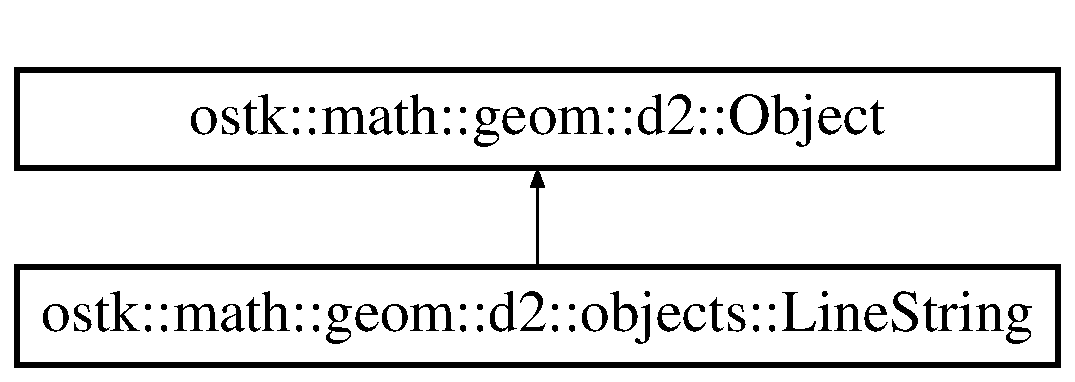
\includegraphics[height=2.000000cm]{classostk_1_1math_1_1geom_1_1d2_1_1objects_1_1_line_string}
\end{center}
\end{figure}
\subsection*{Public Types}
\begin{DoxyCompactItemize}
\item 
typedef Array$<$ \hyperlink{classostk_1_1math_1_1geom_1_1d2_1_1objects_1_1_point}{Point} $>$\+::\hyperlink{classostk_1_1math_1_1geom_1_1d2_1_1objects_1_1_line_string_a29e6326c716bef2ec438534cfdc1e118}{Const\+Iterator} \hyperlink{classostk_1_1math_1_1geom_1_1d2_1_1objects_1_1_line_string_a29e6326c716bef2ec438534cfdc1e118}{Const\+Iterator}
\end{DoxyCompactItemize}
\subsection*{Public Member Functions}
\begin{DoxyCompactItemize}
\item 
\hyperlink{classostk_1_1math_1_1geom_1_1d2_1_1objects_1_1_line_string_ae99b409ec3eddf804a7c83f2452b1249}{Line\+String} (const Array$<$ \hyperlink{classostk_1_1math_1_1geom_1_1d2_1_1objects_1_1_point}{Point} $>$ \&a\+Point\+Array)
\begin{DoxyCompactList}\small\item\em Constructor. \end{DoxyCompactList}\item 
virtual \hyperlink{classostk_1_1math_1_1geom_1_1d2_1_1objects_1_1_line_string}{Line\+String} $\ast$ \hyperlink{classostk_1_1math_1_1geom_1_1d2_1_1objects_1_1_line_string_abb5ac5e7e3e068c6597aab554e6a5e21}{clone} () const override
\begin{DoxyCompactList}\small\item\em Clone line string. \end{DoxyCompactList}\item 
bool \hyperlink{classostk_1_1math_1_1geom_1_1d2_1_1objects_1_1_line_string_ae01ac82c204c56b000f9d531f713c1d1}{operator==} (const \hyperlink{classostk_1_1math_1_1geom_1_1d2_1_1objects_1_1_line_string}{Line\+String} \&a\+Line\+String) const
\begin{DoxyCompactList}\small\item\em Equal to operator. \end{DoxyCompactList}\item 
bool \hyperlink{classostk_1_1math_1_1geom_1_1d2_1_1objects_1_1_line_string_a370337596b70c00beb9c27a0c78462ae}{operator!=} (const \hyperlink{classostk_1_1math_1_1geom_1_1d2_1_1objects_1_1_line_string}{Line\+String} \&a\+Line\+String) const
\begin{DoxyCompactList}\small\item\em Not equal to operator. \end{DoxyCompactList}\item 
virtual bool \hyperlink{classostk_1_1math_1_1geom_1_1d2_1_1objects_1_1_line_string_a0fd7edff5727e1373dbea759313313cc}{is\+Defined} () const override
\begin{DoxyCompactList}\small\item\em Check if line string is defined. \end{DoxyCompactList}\item 
bool \hyperlink{classostk_1_1math_1_1geom_1_1d2_1_1objects_1_1_line_string_a2fe1d6a0a8a917b00b13ab9c3cf24bf3}{is\+Empty} () const
\begin{DoxyCompactList}\small\item\em Check if line string is empty. \end{DoxyCompactList}\item 
bool \hyperlink{classostk_1_1math_1_1geom_1_1d2_1_1objects_1_1_line_string_a04cc661c265dc5777b08754c8015c600}{contains} (const \hyperlink{classostk_1_1math_1_1geom_1_1d2_1_1objects_1_1_point}{Point} \&a\+Point) const
\begin{DoxyCompactList}\small\item\em Check if line string contains a point. \end{DoxyCompactList}\item 
bool \hyperlink{classostk_1_1math_1_1geom_1_1d2_1_1objects_1_1_line_string_a5772e2ac0f24c76d9957e1617077b04a}{is\+Near} (const \hyperlink{classostk_1_1math_1_1geom_1_1d2_1_1objects_1_1_line_string}{Line\+String} \&a\+Line\+String, const Real \&a\+Tolerance) const
\begin{DoxyCompactList}\small\item\em Check if line string is near another line string. \end{DoxyCompactList}\item 
const Array$<$ \hyperlink{classostk_1_1math_1_1geom_1_1d2_1_1objects_1_1_point}{Point} $>$ \& \hyperlink{classostk_1_1math_1_1geom_1_1d2_1_1objects_1_1_line_string_a66969b9cadd8d7b03d3ed1dade26388b}{get\+Point\+Array} () const
\begin{DoxyCompactList}\small\item\em Get point array. \end{DoxyCompactList}\item 
const \hyperlink{classostk_1_1math_1_1geom_1_1d2_1_1objects_1_1_point}{Point} \& \hyperlink{classostk_1_1math_1_1geom_1_1d2_1_1objects_1_1_line_string_a716b6b5f34bbbdcea2a3b4e8e5faf9b5}{access\+Point\+At} (const Index \&an\+Index) const
\begin{DoxyCompactList}\small\item\em Access point at index. \end{DoxyCompactList}\item 
Size \hyperlink{classostk_1_1math_1_1geom_1_1d2_1_1objects_1_1_line_string_af4a7c10fc43a4facff65280e23217ec4}{get\+Point\+Count} () const
\begin{DoxyCompactList}\small\item\em Get point count. \end{DoxyCompactList}\item 
\hyperlink{classostk_1_1math_1_1geom_1_1d2_1_1objects_1_1_point}{Point} \hyperlink{classostk_1_1math_1_1geom_1_1d2_1_1objects_1_1_line_string_adba8e8498cade7e10b4df301b0215d8e}{get\+Point\+Closest\+To} (const \hyperlink{classostk_1_1math_1_1geom_1_1d2_1_1objects_1_1_point}{Point} \&a\+Point) const
\begin{DoxyCompactList}\small\item\em Get point closest to another point. \end{DoxyCompactList}\item 
virtual String \hyperlink{classostk_1_1math_1_1geom_1_1d2_1_1objects_1_1_line_string_a5312030bced48de68f8902bb6581461d}{to\+String} (const \hyperlink{classostk_1_1math_1_1geom_1_1d2_1_1_object_aa76f9e30caebf4005bafbdff447f66cf}{Object\+::\+Format} \&a\+Format=\hyperlink{classostk_1_1math_1_1geom_1_1d2_1_1_object_aa76f9e30caebf4005bafbdff447f66cfaeb6d8ae6f20283755b339c0dc273988b}{Object\+::\+Format\+::\+Standard}, const Integer \&a\+Precision=Integer\+::\+Undefined()) const override
\begin{DoxyCompactList}\small\item\em Get string representation. \end{DoxyCompactList}\item 
virtual void \hyperlink{classostk_1_1math_1_1geom_1_1d2_1_1objects_1_1_line_string_afcdaa3f11f0bd830af0311392c7e9e26}{print} (std\+::ostream \&an\+Output\+Stream, bool display\+Decorators=true) const override
\begin{DoxyCompactList}\small\item\em Print point. \end{DoxyCompactList}\item 
\hyperlink{classostk_1_1math_1_1geom_1_1d2_1_1objects_1_1_line_string_a29e6326c716bef2ec438534cfdc1e118}{Line\+String\+::\+Const\+Iterator} \hyperlink{classostk_1_1math_1_1geom_1_1d2_1_1objects_1_1_line_string_a67bd071017fdd15e96b8930d4e16aacd}{begin} () const
\begin{DoxyCompactList}\small\item\em Get begin const iterator. \end{DoxyCompactList}\item 
\hyperlink{classostk_1_1math_1_1geom_1_1d2_1_1objects_1_1_line_string_a29e6326c716bef2ec438534cfdc1e118}{Line\+String\+::\+Const\+Iterator} \hyperlink{classostk_1_1math_1_1geom_1_1d2_1_1objects_1_1_line_string_ac8336b4c3418337eb1b04f6eb7e11927}{end} () const
\begin{DoxyCompactList}\small\item\em Get end const iterator. \end{DoxyCompactList}\item 
virtual void \hyperlink{classostk_1_1math_1_1geom_1_1d2_1_1objects_1_1_line_string_afd26337c26696a0ff1b4b2e94e58f17c}{apply\+Transformation} (const \hyperlink{classostk_1_1math_1_1geom_1_1d2_1_1_transformation}{Transformation} \&a\+Transformation) override
\begin{DoxyCompactList}\small\item\em Apply transformation to line string. \end{DoxyCompactList}\end{DoxyCompactItemize}
\subsection*{Static Public Member Functions}
\begin{DoxyCompactItemize}
\item 
static \hyperlink{classostk_1_1math_1_1geom_1_1d2_1_1objects_1_1_line_string}{Line\+String} \hyperlink{classostk_1_1math_1_1geom_1_1d2_1_1objects_1_1_line_string_a3557befd15577368d8cc2f9c2a74dfec}{Empty} ()
\begin{DoxyCompactList}\small\item\em Constructs an empty line string. \end{DoxyCompactList}\item 
static \hyperlink{classostk_1_1math_1_1geom_1_1d2_1_1objects_1_1_line_string}{Line\+String} \hyperlink{classostk_1_1math_1_1geom_1_1d2_1_1objects_1_1_line_string_ab95e87bd77782e0a3d50bcd4866d0ec4}{Segment} (const \hyperlink{classostk_1_1math_1_1geom_1_1d2_1_1objects_1_1_segment}{objects\+::\+Segment} \&a\+Segment)
\begin{DoxyCompactList}\small\item\em Constructs a line string from a segment. \end{DoxyCompactList}\end{DoxyCompactItemize}


\subsection{Detailed Description}
\hyperlink{classostk_1_1math_1_1geom_1_1d2_1_1objects_1_1_line}{Line} string. 

A line string is a connected series of line segments.

https\+://en.wikipedia.\+org/wiki/\+Polygonal\+\_\+chain 

\subsection{Member Typedef Documentation}
\mbox{\Hypertarget{classostk_1_1math_1_1geom_1_1d2_1_1objects_1_1_line_string_a29e6326c716bef2ec438534cfdc1e118}\label{classostk_1_1math_1_1geom_1_1d2_1_1objects_1_1_line_string_a29e6326c716bef2ec438534cfdc1e118}} 
\index{ostk\+::math\+::geom\+::d2\+::objects\+::\+Line\+String@{ostk\+::math\+::geom\+::d2\+::objects\+::\+Line\+String}!Const\+Iterator@{Const\+Iterator}}
\index{Const\+Iterator@{Const\+Iterator}!ostk\+::math\+::geom\+::d2\+::objects\+::\+Line\+String@{ostk\+::math\+::geom\+::d2\+::objects\+::\+Line\+String}}
\subsubsection{\texorpdfstring{Const\+Iterator}{ConstIterator}}
{\footnotesize\ttfamily typedef Array$<$\hyperlink{classostk_1_1math_1_1geom_1_1d2_1_1objects_1_1_point}{Point}$>$\+::\hyperlink{classostk_1_1math_1_1geom_1_1d2_1_1objects_1_1_line_string_a29e6326c716bef2ec438534cfdc1e118}{Const\+Iterator} \hyperlink{classostk_1_1math_1_1geom_1_1d2_1_1objects_1_1_line_string_a29e6326c716bef2ec438534cfdc1e118}{ostk\+::math\+::geom\+::d2\+::objects\+::\+Line\+String\+::\+Const\+Iterator}}



\subsection{Constructor \& Destructor Documentation}
\mbox{\Hypertarget{classostk_1_1math_1_1geom_1_1d2_1_1objects_1_1_line_string_ae99b409ec3eddf804a7c83f2452b1249}\label{classostk_1_1math_1_1geom_1_1d2_1_1objects_1_1_line_string_ae99b409ec3eddf804a7c83f2452b1249}} 
\index{ostk\+::math\+::geom\+::d2\+::objects\+::\+Line\+String@{ostk\+::math\+::geom\+::d2\+::objects\+::\+Line\+String}!Line\+String@{Line\+String}}
\index{Line\+String@{Line\+String}!ostk\+::math\+::geom\+::d2\+::objects\+::\+Line\+String@{ostk\+::math\+::geom\+::d2\+::objects\+::\+Line\+String}}
\subsubsection{\texorpdfstring{Line\+String()}{LineString()}}
{\footnotesize\ttfamily ostk\+::math\+::geom\+::d2\+::objects\+::\+Line\+String\+::\+Line\+String (\begin{DoxyParamCaption}\item[{const Array$<$ \hyperlink{classostk_1_1math_1_1geom_1_1d2_1_1objects_1_1_point}{Point} $>$ \&}]{a\+Point\+Array }\end{DoxyParamCaption})}



Constructor. 


\begin{DoxyCode}
\hyperlink{classostk_1_1math_1_1geom_1_1d2_1_1objects_1_1_line_string_ae99b409ec3eddf804a7c83f2452b1249}{LineString} lineString(\{ \{ 0.0, 0.0 \}, \{ 0.0, 1.0 \}, \{ 1.0, 0.0 \} \}) ;
\end{DoxyCode}



\begin{DoxyParams}[1]{Parameters}
\mbox{\tt in}  & {\em a\+Point\+Array} & A point array \\
\hline
\end{DoxyParams}


\subsection{Member Function Documentation}
\mbox{\Hypertarget{classostk_1_1math_1_1geom_1_1d2_1_1objects_1_1_line_string_a716b6b5f34bbbdcea2a3b4e8e5faf9b5}\label{classostk_1_1math_1_1geom_1_1d2_1_1objects_1_1_line_string_a716b6b5f34bbbdcea2a3b4e8e5faf9b5}} 
\index{ostk\+::math\+::geom\+::d2\+::objects\+::\+Line\+String@{ostk\+::math\+::geom\+::d2\+::objects\+::\+Line\+String}!access\+Point\+At@{access\+Point\+At}}
\index{access\+Point\+At@{access\+Point\+At}!ostk\+::math\+::geom\+::d2\+::objects\+::\+Line\+String@{ostk\+::math\+::geom\+::d2\+::objects\+::\+Line\+String}}
\subsubsection{\texorpdfstring{access\+Point\+At()}{accessPointAt()}}
{\footnotesize\ttfamily const \hyperlink{classostk_1_1math_1_1geom_1_1d2_1_1objects_1_1_point}{Point} \& ostk\+::math\+::geom\+::d2\+::objects\+::\+Line\+String\+::access\+Point\+At (\begin{DoxyParamCaption}\item[{const Index \&}]{an\+Index }\end{DoxyParamCaption}) const}



Access point at index. 

\mbox{[}in\mbox{]} an\+Index A point index \begin{DoxyReturn}{Returns}
Reference to point at index 
\end{DoxyReturn}
\mbox{\Hypertarget{classostk_1_1math_1_1geom_1_1d2_1_1objects_1_1_line_string_afd26337c26696a0ff1b4b2e94e58f17c}\label{classostk_1_1math_1_1geom_1_1d2_1_1objects_1_1_line_string_afd26337c26696a0ff1b4b2e94e58f17c}} 
\index{ostk\+::math\+::geom\+::d2\+::objects\+::\+Line\+String@{ostk\+::math\+::geom\+::d2\+::objects\+::\+Line\+String}!apply\+Transformation@{apply\+Transformation}}
\index{apply\+Transformation@{apply\+Transformation}!ostk\+::math\+::geom\+::d2\+::objects\+::\+Line\+String@{ostk\+::math\+::geom\+::d2\+::objects\+::\+Line\+String}}
\subsubsection{\texorpdfstring{apply\+Transformation()}{applyTransformation()}}
{\footnotesize\ttfamily void ostk\+::math\+::geom\+::d2\+::objects\+::\+Line\+String\+::apply\+Transformation (\begin{DoxyParamCaption}\item[{const \hyperlink{classostk_1_1math_1_1geom_1_1d2_1_1_transformation}{Transformation} \&}]{a\+Transformation }\end{DoxyParamCaption})\hspace{0.3cm}{\ttfamily [override]}, {\ttfamily [virtual]}}



Apply transformation to line string. 


\begin{DoxyParams}[1]{Parameters}
\mbox{\tt in}  & {\em a\+Transformation} & A transformation \\
\hline
\end{DoxyParams}


Implements \hyperlink{classostk_1_1math_1_1geom_1_1d2_1_1_object_a959e50211d7a680f7f904bbb752d75c9}{ostk\+::math\+::geom\+::d2\+::\+Object}.

\mbox{\Hypertarget{classostk_1_1math_1_1geom_1_1d2_1_1objects_1_1_line_string_a67bd071017fdd15e96b8930d4e16aacd}\label{classostk_1_1math_1_1geom_1_1d2_1_1objects_1_1_line_string_a67bd071017fdd15e96b8930d4e16aacd}} 
\index{ostk\+::math\+::geom\+::d2\+::objects\+::\+Line\+String@{ostk\+::math\+::geom\+::d2\+::objects\+::\+Line\+String}!begin@{begin}}
\index{begin@{begin}!ostk\+::math\+::geom\+::d2\+::objects\+::\+Line\+String@{ostk\+::math\+::geom\+::d2\+::objects\+::\+Line\+String}}
\subsubsection{\texorpdfstring{begin()}{begin()}}
{\footnotesize\ttfamily \hyperlink{classostk_1_1math_1_1geom_1_1d2_1_1objects_1_1_line_string_a29e6326c716bef2ec438534cfdc1e118}{Line\+String\+::\+Const\+Iterator} ostk\+::math\+::geom\+::d2\+::objects\+::\+Line\+String\+::begin (\begin{DoxyParamCaption}{ }\end{DoxyParamCaption}) const}



Get begin const iterator. 

\begin{DoxyReturn}{Returns}
Begin const iterator 
\end{DoxyReturn}
\mbox{\Hypertarget{classostk_1_1math_1_1geom_1_1d2_1_1objects_1_1_line_string_abb5ac5e7e3e068c6597aab554e6a5e21}\label{classostk_1_1math_1_1geom_1_1d2_1_1objects_1_1_line_string_abb5ac5e7e3e068c6597aab554e6a5e21}} 
\index{ostk\+::math\+::geom\+::d2\+::objects\+::\+Line\+String@{ostk\+::math\+::geom\+::d2\+::objects\+::\+Line\+String}!clone@{clone}}
\index{clone@{clone}!ostk\+::math\+::geom\+::d2\+::objects\+::\+Line\+String@{ostk\+::math\+::geom\+::d2\+::objects\+::\+Line\+String}}
\subsubsection{\texorpdfstring{clone()}{clone()}}
{\footnotesize\ttfamily \hyperlink{classostk_1_1math_1_1geom_1_1d2_1_1objects_1_1_line_string}{Line\+String} $\ast$ ostk\+::math\+::geom\+::d2\+::objects\+::\+Line\+String\+::clone (\begin{DoxyParamCaption}{ }\end{DoxyParamCaption}) const\hspace{0.3cm}{\ttfamily [override]}, {\ttfamily [virtual]}}



Clone line string. 

\begin{DoxyReturn}{Returns}
Pointer to cloned line string 
\end{DoxyReturn}


Implements \hyperlink{classostk_1_1math_1_1geom_1_1d2_1_1_object_a98dedc6792aef35308966ca768eb3e14}{ostk\+::math\+::geom\+::d2\+::\+Object}.

\mbox{\Hypertarget{classostk_1_1math_1_1geom_1_1d2_1_1objects_1_1_line_string_a04cc661c265dc5777b08754c8015c600}\label{classostk_1_1math_1_1geom_1_1d2_1_1objects_1_1_line_string_a04cc661c265dc5777b08754c8015c600}} 
\index{ostk\+::math\+::geom\+::d2\+::objects\+::\+Line\+String@{ostk\+::math\+::geom\+::d2\+::objects\+::\+Line\+String}!contains@{contains}}
\index{contains@{contains}!ostk\+::math\+::geom\+::d2\+::objects\+::\+Line\+String@{ostk\+::math\+::geom\+::d2\+::objects\+::\+Line\+String}}
\subsubsection{\texorpdfstring{contains()}{contains()}}
{\footnotesize\ttfamily bool ostk\+::math\+::geom\+::d2\+::objects\+::\+Line\+String\+::contains (\begin{DoxyParamCaption}\item[{const \hyperlink{classostk_1_1math_1_1geom_1_1d2_1_1objects_1_1_point}{Point} \&}]{a\+Point }\end{DoxyParamCaption}) const}



Check if line string contains a point. 


\begin{DoxyCode}
\hyperlink{classostk_1_1math_1_1geom_1_1d2_1_1objects_1_1_line_string_ae99b409ec3eddf804a7c83f2452b1249}{LineString}(\{ \{ 0.0, 0.0 \}, \{ 0.0, 1.0 \}, \{ 1.0, 0.0 \} \}).\hyperlink{classostk_1_1math_1_1geom_1_1d2_1_1objects_1_1_line_string_a04cc661c265dc5777b08754c8015c600}{contains}(\{ 0.0, 0.5 \}) ; \textcolor{comment}{// True}
\end{DoxyCode}


\begin{DoxyReturn}{Returns}
True if line string contains a point 
\end{DoxyReturn}
\mbox{\Hypertarget{classostk_1_1math_1_1geom_1_1d2_1_1objects_1_1_line_string_a3557befd15577368d8cc2f9c2a74dfec}\label{classostk_1_1math_1_1geom_1_1d2_1_1objects_1_1_line_string_a3557befd15577368d8cc2f9c2a74dfec}} 
\index{ostk\+::math\+::geom\+::d2\+::objects\+::\+Line\+String@{ostk\+::math\+::geom\+::d2\+::objects\+::\+Line\+String}!Empty@{Empty}}
\index{Empty@{Empty}!ostk\+::math\+::geom\+::d2\+::objects\+::\+Line\+String@{ostk\+::math\+::geom\+::d2\+::objects\+::\+Line\+String}}
\subsubsection{\texorpdfstring{Empty()}{Empty()}}
{\footnotesize\ttfamily \hyperlink{classostk_1_1math_1_1geom_1_1d2_1_1objects_1_1_line_string}{Line\+String} ostk\+::math\+::geom\+::d2\+::objects\+::\+Line\+String\+::\+Empty (\begin{DoxyParamCaption}{ }\end{DoxyParamCaption})\hspace{0.3cm}{\ttfamily [static]}}



Constructs an empty line string. 


\begin{DoxyCode}
\hyperlink{classostk_1_1math_1_1geom_1_1d2_1_1objects_1_1_line_string_ae99b409ec3eddf804a7c83f2452b1249}{LineString} lineString = \hyperlink{classostk_1_1math_1_1geom_1_1d2_1_1objects_1_1_line_string_a3557befd15577368d8cc2f9c2a74dfec}{LineString::Empty}() ;
\end{DoxyCode}


\begin{DoxyReturn}{Returns}
Empty line string 
\end{DoxyReturn}
\mbox{\Hypertarget{classostk_1_1math_1_1geom_1_1d2_1_1objects_1_1_line_string_ac8336b4c3418337eb1b04f6eb7e11927}\label{classostk_1_1math_1_1geom_1_1d2_1_1objects_1_1_line_string_ac8336b4c3418337eb1b04f6eb7e11927}} 
\index{ostk\+::math\+::geom\+::d2\+::objects\+::\+Line\+String@{ostk\+::math\+::geom\+::d2\+::objects\+::\+Line\+String}!end@{end}}
\index{end@{end}!ostk\+::math\+::geom\+::d2\+::objects\+::\+Line\+String@{ostk\+::math\+::geom\+::d2\+::objects\+::\+Line\+String}}
\subsubsection{\texorpdfstring{end()}{end()}}
{\footnotesize\ttfamily \hyperlink{classostk_1_1math_1_1geom_1_1d2_1_1objects_1_1_line_string_a29e6326c716bef2ec438534cfdc1e118}{Line\+String\+::\+Const\+Iterator} ostk\+::math\+::geom\+::d2\+::objects\+::\+Line\+String\+::end (\begin{DoxyParamCaption}{ }\end{DoxyParamCaption}) const}



Get end const iterator. 

\begin{DoxyReturn}{Returns}
End const iterator 
\end{DoxyReturn}
\mbox{\Hypertarget{classostk_1_1math_1_1geom_1_1d2_1_1objects_1_1_line_string_a66969b9cadd8d7b03d3ed1dade26388b}\label{classostk_1_1math_1_1geom_1_1d2_1_1objects_1_1_line_string_a66969b9cadd8d7b03d3ed1dade26388b}} 
\index{ostk\+::math\+::geom\+::d2\+::objects\+::\+Line\+String@{ostk\+::math\+::geom\+::d2\+::objects\+::\+Line\+String}!get\+Point\+Array@{get\+Point\+Array}}
\index{get\+Point\+Array@{get\+Point\+Array}!ostk\+::math\+::geom\+::d2\+::objects\+::\+Line\+String@{ostk\+::math\+::geom\+::d2\+::objects\+::\+Line\+String}}
\subsubsection{\texorpdfstring{get\+Point\+Array()}{getPointArray()}}
{\footnotesize\ttfamily const Array$<$ \hyperlink{classostk_1_1math_1_1geom_1_1d2_1_1objects_1_1_point}{Point} $>$ \& ostk\+::math\+::geom\+::d2\+::objects\+::\+Line\+String\+::get\+Point\+Array (\begin{DoxyParamCaption}{ }\end{DoxyParamCaption}) const}



Get point array. 

\begin{DoxyReturn}{Returns}
\hyperlink{classostk_1_1math_1_1geom_1_1d2_1_1objects_1_1_point}{Point} array 
\end{DoxyReturn}
\mbox{\Hypertarget{classostk_1_1math_1_1geom_1_1d2_1_1objects_1_1_line_string_adba8e8498cade7e10b4df301b0215d8e}\label{classostk_1_1math_1_1geom_1_1d2_1_1objects_1_1_line_string_adba8e8498cade7e10b4df301b0215d8e}} 
\index{ostk\+::math\+::geom\+::d2\+::objects\+::\+Line\+String@{ostk\+::math\+::geom\+::d2\+::objects\+::\+Line\+String}!get\+Point\+Closest\+To@{get\+Point\+Closest\+To}}
\index{get\+Point\+Closest\+To@{get\+Point\+Closest\+To}!ostk\+::math\+::geom\+::d2\+::objects\+::\+Line\+String@{ostk\+::math\+::geom\+::d2\+::objects\+::\+Line\+String}}
\subsubsection{\texorpdfstring{get\+Point\+Closest\+To()}{getPointClosestTo()}}
{\footnotesize\ttfamily \hyperlink{classostk_1_1math_1_1geom_1_1d2_1_1objects_1_1_point}{Point} ostk\+::math\+::geom\+::d2\+::objects\+::\+Line\+String\+::get\+Point\+Closest\+To (\begin{DoxyParamCaption}\item[{const \hyperlink{classostk_1_1math_1_1geom_1_1d2_1_1objects_1_1_point}{Point} \&}]{a\+Point }\end{DoxyParamCaption}) const}



Get point closest to another point. 


\begin{DoxyParams}[1]{Parameters}
\mbox{\tt in}  & {\em a\+Point} & A point \\
\hline
\end{DoxyParams}
\begin{DoxyReturn}{Returns}
Closest point 
\end{DoxyReturn}
\mbox{\Hypertarget{classostk_1_1math_1_1geom_1_1d2_1_1objects_1_1_line_string_af4a7c10fc43a4facff65280e23217ec4}\label{classostk_1_1math_1_1geom_1_1d2_1_1objects_1_1_line_string_af4a7c10fc43a4facff65280e23217ec4}} 
\index{ostk\+::math\+::geom\+::d2\+::objects\+::\+Line\+String@{ostk\+::math\+::geom\+::d2\+::objects\+::\+Line\+String}!get\+Point\+Count@{get\+Point\+Count}}
\index{get\+Point\+Count@{get\+Point\+Count}!ostk\+::math\+::geom\+::d2\+::objects\+::\+Line\+String@{ostk\+::math\+::geom\+::d2\+::objects\+::\+Line\+String}}
\subsubsection{\texorpdfstring{get\+Point\+Count()}{getPointCount()}}
{\footnotesize\ttfamily Size ostk\+::math\+::geom\+::d2\+::objects\+::\+Line\+String\+::get\+Point\+Count (\begin{DoxyParamCaption}{ }\end{DoxyParamCaption}) const}



Get point count. 

\begin{DoxyReturn}{Returns}
\hyperlink{classostk_1_1math_1_1geom_1_1d2_1_1objects_1_1_point}{Point} count 
\end{DoxyReturn}
\mbox{\Hypertarget{classostk_1_1math_1_1geom_1_1d2_1_1objects_1_1_line_string_a0fd7edff5727e1373dbea759313313cc}\label{classostk_1_1math_1_1geom_1_1d2_1_1objects_1_1_line_string_a0fd7edff5727e1373dbea759313313cc}} 
\index{ostk\+::math\+::geom\+::d2\+::objects\+::\+Line\+String@{ostk\+::math\+::geom\+::d2\+::objects\+::\+Line\+String}!is\+Defined@{is\+Defined}}
\index{is\+Defined@{is\+Defined}!ostk\+::math\+::geom\+::d2\+::objects\+::\+Line\+String@{ostk\+::math\+::geom\+::d2\+::objects\+::\+Line\+String}}
\subsubsection{\texorpdfstring{is\+Defined()}{isDefined()}}
{\footnotesize\ttfamily bool ostk\+::math\+::geom\+::d2\+::objects\+::\+Line\+String\+::is\+Defined (\begin{DoxyParamCaption}{ }\end{DoxyParamCaption}) const\hspace{0.3cm}{\ttfamily [override]}, {\ttfamily [virtual]}}



Check if line string is defined. 


\begin{DoxyCode}
\hyperlink{classostk_1_1math_1_1geom_1_1d2_1_1objects_1_1_line_string_ae99b409ec3eddf804a7c83f2452b1249}{LineString}(0.0, 0.0).isDefined() ; \textcolor{comment}{// True}
\end{DoxyCode}


\begin{DoxyReturn}{Returns}
True if line string is defined 
\end{DoxyReturn}


Implements \hyperlink{classostk_1_1math_1_1geom_1_1d2_1_1_object_a456cc7121218d24c1322d0fe54230cc4}{ostk\+::math\+::geom\+::d2\+::\+Object}.

\mbox{\Hypertarget{classostk_1_1math_1_1geom_1_1d2_1_1objects_1_1_line_string_a2fe1d6a0a8a917b00b13ab9c3cf24bf3}\label{classostk_1_1math_1_1geom_1_1d2_1_1objects_1_1_line_string_a2fe1d6a0a8a917b00b13ab9c3cf24bf3}} 
\index{ostk\+::math\+::geom\+::d2\+::objects\+::\+Line\+String@{ostk\+::math\+::geom\+::d2\+::objects\+::\+Line\+String}!is\+Empty@{is\+Empty}}
\index{is\+Empty@{is\+Empty}!ostk\+::math\+::geom\+::d2\+::objects\+::\+Line\+String@{ostk\+::math\+::geom\+::d2\+::objects\+::\+Line\+String}}
\subsubsection{\texorpdfstring{is\+Empty()}{isEmpty()}}
{\footnotesize\ttfamily bool ostk\+::math\+::geom\+::d2\+::objects\+::\+Line\+String\+::is\+Empty (\begin{DoxyParamCaption}{ }\end{DoxyParamCaption}) const}



Check if line string is empty. 


\begin{DoxyCode}
\hyperlink{classostk_1_1math_1_1geom_1_1d2_1_1objects_1_1_line_string_a3557befd15577368d8cc2f9c2a74dfec}{LineString::Empty}().\hyperlink{classostk_1_1math_1_1geom_1_1d2_1_1objects_1_1_line_string_a2fe1d6a0a8a917b00b13ab9c3cf24bf3}{isEmpty}() ; \textcolor{comment}{// True}
\end{DoxyCode}


\begin{DoxyReturn}{Returns}
True if line string is empty 
\end{DoxyReturn}
\mbox{\Hypertarget{classostk_1_1math_1_1geom_1_1d2_1_1objects_1_1_line_string_a5772e2ac0f24c76d9957e1617077b04a}\label{classostk_1_1math_1_1geom_1_1d2_1_1objects_1_1_line_string_a5772e2ac0f24c76d9957e1617077b04a}} 
\index{ostk\+::math\+::geom\+::d2\+::objects\+::\+Line\+String@{ostk\+::math\+::geom\+::d2\+::objects\+::\+Line\+String}!is\+Near@{is\+Near}}
\index{is\+Near@{is\+Near}!ostk\+::math\+::geom\+::d2\+::objects\+::\+Line\+String@{ostk\+::math\+::geom\+::d2\+::objects\+::\+Line\+String}}
\subsubsection{\texorpdfstring{is\+Near()}{isNear()}}
{\footnotesize\ttfamily bool ostk\+::math\+::geom\+::d2\+::objects\+::\+Line\+String\+::is\+Near (\begin{DoxyParamCaption}\item[{const \hyperlink{classostk_1_1math_1_1geom_1_1d2_1_1objects_1_1_line_string}{Line\+String} \&}]{a\+Line\+String,  }\item[{const Real \&}]{a\+Tolerance }\end{DoxyParamCaption}) const}



Check if line string is near another line string. 


\begin{DoxyCode}
\hyperlink{classostk_1_1math_1_1geom_1_1d2_1_1objects_1_1_line_string_ae99b409ec3eddf804a7c83f2452b1249}{LineString}(\{ \{ 0.0, 0.0 \}, \{ 0.0, 1.0 \}, \{ 1.0, 0.0 \} \}).\hyperlink{classostk_1_1math_1_1geom_1_1d2_1_1objects_1_1_line_string_a5772e2ac0f24c76d9957e1617077b04a}{isNear}(
      \hyperlink{classostk_1_1math_1_1geom_1_1d2_1_1objects_1_1_line_string_ae99b409ec3eddf804a7c83f2452b1249}{LineString}(\{ \{ 0.0, 0.0 \}, \{ 0.0, 1.0 \}, \{ 1.0, 1e-15 \} \}), 1e-15) ; \textcolor{comment}{// True}
\end{DoxyCode}



\begin{DoxyParams}[1]{Parameters}
\mbox{\tt in}  & {\em a\+Line\+String} & A line string \\
\hline
\mbox{\tt in}  & {\em a\+Tolerance} & A tolerance \\
\hline
\end{DoxyParams}
\begin{DoxyReturn}{Returns}
True if line string is near another line string 
\end{DoxyReturn}
\mbox{\Hypertarget{classostk_1_1math_1_1geom_1_1d2_1_1objects_1_1_line_string_a370337596b70c00beb9c27a0c78462ae}\label{classostk_1_1math_1_1geom_1_1d2_1_1objects_1_1_line_string_a370337596b70c00beb9c27a0c78462ae}} 
\index{ostk\+::math\+::geom\+::d2\+::objects\+::\+Line\+String@{ostk\+::math\+::geom\+::d2\+::objects\+::\+Line\+String}!operator"!=@{operator"!=}}
\index{operator"!=@{operator"!=}!ostk\+::math\+::geom\+::d2\+::objects\+::\+Line\+String@{ostk\+::math\+::geom\+::d2\+::objects\+::\+Line\+String}}
\subsubsection{\texorpdfstring{operator"!=()}{operator!=()}}
{\footnotesize\ttfamily bool ostk\+::math\+::geom\+::d2\+::objects\+::\+Line\+String\+::operator!= (\begin{DoxyParamCaption}\item[{const \hyperlink{classostk_1_1math_1_1geom_1_1d2_1_1objects_1_1_line_string}{Line\+String} \&}]{a\+Line\+String }\end{DoxyParamCaption}) const}



Not equal to operator. 


\begin{DoxyParams}[1]{Parameters}
\mbox{\tt in}  & {\em a\+Line\+String} & A line string \\
\hline
\end{DoxyParams}
\begin{DoxyReturn}{Returns}
True if line strings are not equal 
\end{DoxyReturn}
\mbox{\Hypertarget{classostk_1_1math_1_1geom_1_1d2_1_1objects_1_1_line_string_ae01ac82c204c56b000f9d531f713c1d1}\label{classostk_1_1math_1_1geom_1_1d2_1_1objects_1_1_line_string_ae01ac82c204c56b000f9d531f713c1d1}} 
\index{ostk\+::math\+::geom\+::d2\+::objects\+::\+Line\+String@{ostk\+::math\+::geom\+::d2\+::objects\+::\+Line\+String}!operator==@{operator==}}
\index{operator==@{operator==}!ostk\+::math\+::geom\+::d2\+::objects\+::\+Line\+String@{ostk\+::math\+::geom\+::d2\+::objects\+::\+Line\+String}}
\subsubsection{\texorpdfstring{operator==()}{operator==()}}
{\footnotesize\ttfamily bool ostk\+::math\+::geom\+::d2\+::objects\+::\+Line\+String\+::operator== (\begin{DoxyParamCaption}\item[{const \hyperlink{classostk_1_1math_1_1geom_1_1d2_1_1objects_1_1_line_string}{Line\+String} \&}]{a\+Line\+String }\end{DoxyParamCaption}) const}



Equal to operator. 


\begin{DoxyParams}[1]{Parameters}
\mbox{\tt in}  & {\em a\+Line\+String} & A line string \\
\hline
\end{DoxyParams}
\begin{DoxyReturn}{Returns}
True if line strings are equal 
\end{DoxyReturn}
\mbox{\Hypertarget{classostk_1_1math_1_1geom_1_1d2_1_1objects_1_1_line_string_afcdaa3f11f0bd830af0311392c7e9e26}\label{classostk_1_1math_1_1geom_1_1d2_1_1objects_1_1_line_string_afcdaa3f11f0bd830af0311392c7e9e26}} 
\index{ostk\+::math\+::geom\+::d2\+::objects\+::\+Line\+String@{ostk\+::math\+::geom\+::d2\+::objects\+::\+Line\+String}!print@{print}}
\index{print@{print}!ostk\+::math\+::geom\+::d2\+::objects\+::\+Line\+String@{ostk\+::math\+::geom\+::d2\+::objects\+::\+Line\+String}}
\subsubsection{\texorpdfstring{print()}{print()}}
{\footnotesize\ttfamily void ostk\+::math\+::geom\+::d2\+::objects\+::\+Line\+String\+::print (\begin{DoxyParamCaption}\item[{std\+::ostream \&}]{an\+Output\+Stream,  }\item[{bool}]{display\+Decorators = {\ttfamily true} }\end{DoxyParamCaption}) const\hspace{0.3cm}{\ttfamily [override]}, {\ttfamily [virtual]}}



Print point. 


\begin{DoxyParams}[1]{Parameters}
\mbox{\tt in}  & {\em an\+Output\+Stream} & An output stream \\
\hline
\mbox{\tt in}  & {\em (optional)} & display\+Decorators If true, display decorators \\
\hline
\end{DoxyParams}


Implements \hyperlink{classostk_1_1math_1_1geom_1_1d2_1_1_object_ae05ad883ed5a560e38f0aae7a4adc1ea}{ostk\+::math\+::geom\+::d2\+::\+Object}.

\mbox{\Hypertarget{classostk_1_1math_1_1geom_1_1d2_1_1objects_1_1_line_string_ab95e87bd77782e0a3d50bcd4866d0ec4}\label{classostk_1_1math_1_1geom_1_1d2_1_1objects_1_1_line_string_ab95e87bd77782e0a3d50bcd4866d0ec4}} 
\index{ostk\+::math\+::geom\+::d2\+::objects\+::\+Line\+String@{ostk\+::math\+::geom\+::d2\+::objects\+::\+Line\+String}!Segment@{Segment}}
\index{Segment@{Segment}!ostk\+::math\+::geom\+::d2\+::objects\+::\+Line\+String@{ostk\+::math\+::geom\+::d2\+::objects\+::\+Line\+String}}
\subsubsection{\texorpdfstring{Segment()}{Segment()}}
{\footnotesize\ttfamily \hyperlink{classostk_1_1math_1_1geom_1_1d2_1_1objects_1_1_line_string}{Line\+String} ostk\+::math\+::geom\+::d2\+::objects\+::\+Line\+String\+::\+Segment (\begin{DoxyParamCaption}\item[{const \hyperlink{classostk_1_1math_1_1geom_1_1d2_1_1objects_1_1_segment}{objects\+::\+Segment} \&}]{a\+Segment }\end{DoxyParamCaption})\hspace{0.3cm}{\ttfamily [static]}}



Constructs a line string from a segment. 


\begin{DoxyCode}
\hyperlink{classostk_1_1math_1_1geom_1_1d2_1_1objects_1_1_line_string_ab95e87bd77782e0a3d50bcd4866d0ec4}{Segment} segment = \{ \{ 0.0, 0.0 \}, \{ 0.0, 1.0 \} \} ;
\hyperlink{classostk_1_1math_1_1geom_1_1d2_1_1objects_1_1_line_string_ae99b409ec3eddf804a7c83f2452b1249}{LineString} lineString = \hyperlink{classostk_1_1math_1_1geom_1_1d2_1_1objects_1_1_line_string_ab95e87bd77782e0a3d50bcd4866d0ec4}{LineString::Segment}(segment) ;
\end{DoxyCode}


\begin{DoxyReturn}{Returns}
\hyperlink{classostk_1_1math_1_1geom_1_1d2_1_1objects_1_1_line}{Line} string 
\end{DoxyReturn}
\mbox{\Hypertarget{classostk_1_1math_1_1geom_1_1d2_1_1objects_1_1_line_string_a5312030bced48de68f8902bb6581461d}\label{classostk_1_1math_1_1geom_1_1d2_1_1objects_1_1_line_string_a5312030bced48de68f8902bb6581461d}} 
\index{ostk\+::math\+::geom\+::d2\+::objects\+::\+Line\+String@{ostk\+::math\+::geom\+::d2\+::objects\+::\+Line\+String}!to\+String@{to\+String}}
\index{to\+String@{to\+String}!ostk\+::math\+::geom\+::d2\+::objects\+::\+Line\+String@{ostk\+::math\+::geom\+::d2\+::objects\+::\+Line\+String}}
\subsubsection{\texorpdfstring{to\+String()}{toString()}}
{\footnotesize\ttfamily String ostk\+::math\+::geom\+::d2\+::objects\+::\+Line\+String\+::to\+String (\begin{DoxyParamCaption}\item[{const \hyperlink{classostk_1_1math_1_1geom_1_1d2_1_1_object_aa76f9e30caebf4005bafbdff447f66cf}{Object\+::\+Format} \&}]{a\+Format = {\ttfamily \hyperlink{classostk_1_1math_1_1geom_1_1d2_1_1_object_aa76f9e30caebf4005bafbdff447f66cfaeb6d8ae6f20283755b339c0dc273988b}{Object\+::\+Format\+::\+Standard}},  }\item[{const Integer \&}]{a\+Precision = {\ttfamily Integer\+:\+:Undefined()} }\end{DoxyParamCaption}) const\hspace{0.3cm}{\ttfamily [override]}, {\ttfamily [virtual]}}



Get string representation. 


\begin{DoxyParams}[1]{Parameters}
\mbox{\tt in}  & {\em a\+Format} & A format \\
\hline
\end{DoxyParams}
\begin{DoxyReturn}{Returns}
String representation 
\end{DoxyReturn}


Implements \hyperlink{classostk_1_1math_1_1geom_1_1d2_1_1_object_ada4c2187dd24ef02b91b6346191f677c}{ostk\+::math\+::geom\+::d2\+::\+Object}.



The documentation for this class was generated from the following files\+:\begin{DoxyCompactItemize}
\item 
include/\+Open\+Space\+Toolkit/\+Mathematics/\+Geometry/2\+D/\+Objects/\hyperlink{2_d_2_objects_2_line_string_8hpp}{Line\+String.\+hpp}\item 
src/\+Open\+Space\+Toolkit/\+Mathematics/\+Geometry/2\+D/\+Objects/\hyperlink{2_d_2_objects_2_line_string_8cpp}{Line\+String.\+cpp}\end{DoxyCompactItemize}

\hypertarget{classostk_1_1math_1_1geom_1_1d2_1_1objects_1_1_multi_line_string}{}\doxysection{ostk\+::math\+::geom\+::d2\+::objects\+::Multi\+Line\+String Class Reference}
\label{classostk_1_1math_1_1geom_1_1d2_1_1objects_1_1_multi_line_string}\index{ostk::math::geom::d2::objects::MultiLineString@{ostk::math::geom::d2::objects::MultiLineString}}


Multi \mbox{\hyperlink{classostk_1_1math_1_1geom_1_1d2_1_1objects_1_1_line}{Line}} string.  




{\ttfamily \#include $<$Multi\+Line\+String.\+hpp$>$}

Inheritance diagram for ostk\+::math\+::geom\+::d2\+::objects\+::Multi\+Line\+String\+:\begin{figure}[H]
\begin{center}
\leavevmode
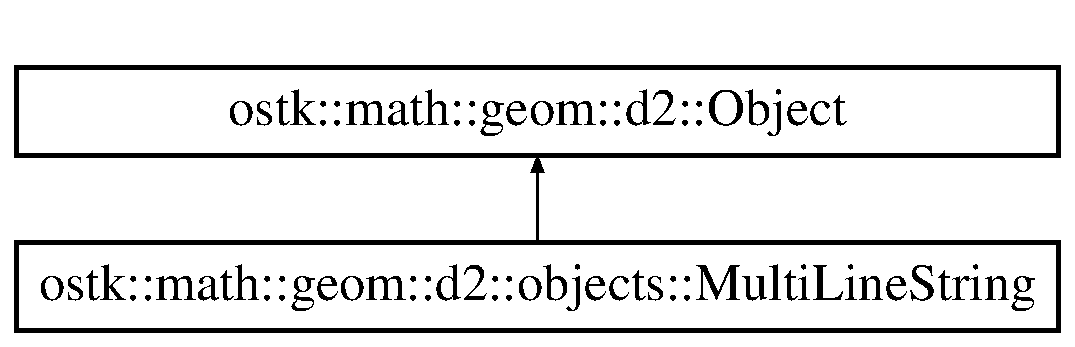
\includegraphics[height=2.000000cm]{classostk_1_1math_1_1geom_1_1d2_1_1objects_1_1_multi_line_string}
\end{center}
\end{figure}
\doxysubsection*{Public Types}
\begin{DoxyCompactItemize}
\item 
typedef Array$<$ \mbox{\hyperlink{classostk_1_1math_1_1geom_1_1d2_1_1objects_1_1_line_string}{Line\+String}} $>$\+::\mbox{\hyperlink{classostk_1_1math_1_1geom_1_1d2_1_1objects_1_1_multi_line_string_a43dc9419e5743d8a920141ba4fa10c5f}{Const\+Iterator}} \mbox{\hyperlink{classostk_1_1math_1_1geom_1_1d2_1_1objects_1_1_multi_line_string_a43dc9419e5743d8a920141ba4fa10c5f}{Const\+Iterator}}
\end{DoxyCompactItemize}
\doxysubsection*{Public Member Functions}
\begin{DoxyCompactItemize}
\item 
\mbox{\hyperlink{classostk_1_1math_1_1geom_1_1d2_1_1objects_1_1_multi_line_string_a5a30febbcbc28097e34b6f2f3f456b79}{Multi\+Line\+String}} (const Array$<$ \mbox{\hyperlink{classostk_1_1math_1_1geom_1_1d2_1_1objects_1_1_line_string}{Line\+String}} $>$ \&a\+Line\+String\+Array)
\begin{DoxyCompactList}\small\item\em Constructor. \end{DoxyCompactList}\item 
virtual \mbox{\hyperlink{classostk_1_1math_1_1geom_1_1d2_1_1objects_1_1_multi_line_string}{Multi\+Line\+String}} $\ast$ \mbox{\hyperlink{classostk_1_1math_1_1geom_1_1d2_1_1objects_1_1_multi_line_string_abf1b39f7e7f9c1f1ba9b040669863e81}{clone}} () const override
\begin{DoxyCompactList}\small\item\em Clone multi line string. \end{DoxyCompactList}\item 
bool \mbox{\hyperlink{classostk_1_1math_1_1geom_1_1d2_1_1objects_1_1_multi_line_string_af0bbb61f35a16ac8c61283221d2ddc43}{operator==}} (const \mbox{\hyperlink{classostk_1_1math_1_1geom_1_1d2_1_1objects_1_1_multi_line_string}{Multi\+Line\+String}} \&a\+Multi\+Line\+String) const
\begin{DoxyCompactList}\small\item\em Equal to operator. \end{DoxyCompactList}\item 
bool \mbox{\hyperlink{classostk_1_1math_1_1geom_1_1d2_1_1objects_1_1_multi_line_string_a124780190c563f303f81bff8e25ed742}{operator!=}} (const \mbox{\hyperlink{classostk_1_1math_1_1geom_1_1d2_1_1objects_1_1_multi_line_string}{Multi\+Line\+String}} \&a\+Multi\+Line\+String) const
\begin{DoxyCompactList}\small\item\em Not equal to operator. \end{DoxyCompactList}\item 
virtual bool \mbox{\hyperlink{classostk_1_1math_1_1geom_1_1d2_1_1objects_1_1_multi_line_string_a446d9d1344336d6ec8b2ff1e46629ca2}{is\+Defined}} () const override
\begin{DoxyCompactList}\small\item\em Check if multi multi line string is defined. \end{DoxyCompactList}\item 
bool \mbox{\hyperlink{classostk_1_1math_1_1geom_1_1d2_1_1objects_1_1_multi_line_string_a5d9130266958b3cddbcfd9ac085074f9}{is\+Empty}} () const
\begin{DoxyCompactList}\small\item\em Check if multi multi line string is empty. \end{DoxyCompactList}\item 
Size \mbox{\hyperlink{classostk_1_1math_1_1geom_1_1d2_1_1objects_1_1_multi_line_string_ad4bf5470a4824babbe4fb314b58537a0}{get\+Line\+String\+Count}} () const
\begin{DoxyCompactList}\small\item\em Get multi line string count. \end{DoxyCompactList}\item 
Size \mbox{\hyperlink{classostk_1_1math_1_1geom_1_1d2_1_1objects_1_1_multi_line_string_a79be04f2c6bddfa1689b6eefba45fc83}{get\+Point\+Count}} () const
\begin{DoxyCompactList}\small\item\em Get point count. \end{DoxyCompactList}\item 
\mbox{\hyperlink{classostk_1_1math_1_1geom_1_1d2_1_1objects_1_1_point}{Point}} \mbox{\hyperlink{classostk_1_1math_1_1geom_1_1d2_1_1objects_1_1_multi_line_string_ad8b2805d38191a13711bd7255ea48e9f}{get\+Point\+Closest\+To}} (const \mbox{\hyperlink{classostk_1_1math_1_1geom_1_1d2_1_1objects_1_1_point}{Point}} \&a\+Point) const
\begin{DoxyCompactList}\small\item\em Get point closest to another point. \end{DoxyCompactList}\item 
virtual String \mbox{\hyperlink{classostk_1_1math_1_1geom_1_1d2_1_1objects_1_1_multi_line_string_a87df673d41e16eb2b196c8b8a852d71f}{to\+String}} (const \mbox{\hyperlink{classostk_1_1math_1_1geom_1_1d2_1_1_object_aa76f9e30caebf4005bafbdff447f66cf}{Object\+::\+Format}} \&a\+Format=\mbox{\hyperlink{classostk_1_1math_1_1geom_1_1d2_1_1_object_aa76f9e30caebf4005bafbdff447f66cfaeb6d8ae6f20283755b339c0dc273988b}{Object\+::\+Format\+::\+Standard}}, const Integer \&a\+Precision=Integer\+::\+Undefined()) const override
\begin{DoxyCompactList}\small\item\em Get string representation. \end{DoxyCompactList}\item 
virtual void \mbox{\hyperlink{classostk_1_1math_1_1geom_1_1d2_1_1objects_1_1_multi_line_string_a5e90edd640ee9262194eb07d943bb8bb}{print}} (std\+::ostream \&an\+Output\+Stream, bool display\+Decorators=true) const override
\begin{DoxyCompactList}\small\item\em Print point. \end{DoxyCompactList}\item 
\mbox{\hyperlink{classostk_1_1math_1_1geom_1_1d2_1_1objects_1_1_multi_line_string_a43dc9419e5743d8a920141ba4fa10c5f}{Multi\+Line\+String\+::\+Const\+Iterator}} \mbox{\hyperlink{classostk_1_1math_1_1geom_1_1d2_1_1objects_1_1_multi_line_string_a9789bc63ef669a8f625da8f617a605a6}{begin}} () const
\begin{DoxyCompactList}\small\item\em Get begin const iterator. \end{DoxyCompactList}\item 
\mbox{\hyperlink{classostk_1_1math_1_1geom_1_1d2_1_1objects_1_1_multi_line_string_a43dc9419e5743d8a920141ba4fa10c5f}{Multi\+Line\+String\+::\+Const\+Iterator}} \mbox{\hyperlink{classostk_1_1math_1_1geom_1_1d2_1_1objects_1_1_multi_line_string_ac2e17ceb1a3f276273c5276a5d0a4ea2}{end}} () const
\begin{DoxyCompactList}\small\item\em Get end const iterator. \end{DoxyCompactList}\item 
virtual void \mbox{\hyperlink{classostk_1_1math_1_1geom_1_1d2_1_1objects_1_1_multi_line_string_ada5fe5a183b6628831867b416901459e}{apply\+Transformation}} (const \mbox{\hyperlink{classostk_1_1math_1_1geom_1_1d2_1_1_transformation}{Transformation}} \&a\+Transformation) override
\begin{DoxyCompactList}\small\item\em Apply transformation to multi line string. \end{DoxyCompactList}\end{DoxyCompactItemize}
\doxysubsection*{Static Public Member Functions}
\begin{DoxyCompactItemize}
\item 
static \mbox{\hyperlink{classostk_1_1math_1_1geom_1_1d2_1_1objects_1_1_multi_line_string}{Multi\+Line\+String}} \mbox{\hyperlink{classostk_1_1math_1_1geom_1_1d2_1_1objects_1_1_multi_line_string_a1f0815649194309c185ac3020b9d80a2}{Empty}} ()
\begin{DoxyCompactList}\small\item\em Constructs an empty multi line string. \end{DoxyCompactList}\end{DoxyCompactItemize}


\doxysubsection{Detailed Description}
Multi \mbox{\hyperlink{classostk_1_1math_1_1geom_1_1d2_1_1objects_1_1_line}{Line}} string. 

\doxysubsection{Member Typedef Documentation}
\mbox{\Hypertarget{classostk_1_1math_1_1geom_1_1d2_1_1objects_1_1_multi_line_string_a43dc9419e5743d8a920141ba4fa10c5f}\label{classostk_1_1math_1_1geom_1_1d2_1_1objects_1_1_multi_line_string_a43dc9419e5743d8a920141ba4fa10c5f}} 
\index{ostk::math::geom::d2::objects::MultiLineString@{ostk::math::geom::d2::objects::MultiLineString}!ConstIterator@{ConstIterator}}
\index{ConstIterator@{ConstIterator}!ostk::math::geom::d2::objects::MultiLineString@{ostk::math::geom::d2::objects::MultiLineString}}
\doxysubsubsection{\texorpdfstring{ConstIterator}{ConstIterator}}
{\footnotesize\ttfamily typedef Array$<$\mbox{\hyperlink{classostk_1_1math_1_1geom_1_1d2_1_1objects_1_1_line_string}{Line\+String}}$>$\+::\mbox{\hyperlink{classostk_1_1math_1_1geom_1_1d2_1_1objects_1_1_multi_line_string_a43dc9419e5743d8a920141ba4fa10c5f}{Const\+Iterator}} \mbox{\hyperlink{classostk_1_1math_1_1geom_1_1d2_1_1objects_1_1_multi_line_string_a43dc9419e5743d8a920141ba4fa10c5f}{ostk\+::math\+::geom\+::d2\+::objects\+::\+Multi\+Line\+String\+::\+Const\+Iterator}}}



\doxysubsection{Constructor \& Destructor Documentation}
\mbox{\Hypertarget{classostk_1_1math_1_1geom_1_1d2_1_1objects_1_1_multi_line_string_a5a30febbcbc28097e34b6f2f3f456b79}\label{classostk_1_1math_1_1geom_1_1d2_1_1objects_1_1_multi_line_string_a5a30febbcbc28097e34b6f2f3f456b79}} 
\index{ostk::math::geom::d2::objects::MultiLineString@{ostk::math::geom::d2::objects::MultiLineString}!MultiLineString@{MultiLineString}}
\index{MultiLineString@{MultiLineString}!ostk::math::geom::d2::objects::MultiLineString@{ostk::math::geom::d2::objects::MultiLineString}}
\doxysubsubsection{\texorpdfstring{MultiLineString()}{MultiLineString()}}
{\footnotesize\ttfamily ostk\+::math\+::geom\+::d2\+::objects\+::\+Multi\+Line\+String\+::\+Multi\+Line\+String (\begin{DoxyParamCaption}\item[{const Array$<$ \mbox{\hyperlink{classostk_1_1math_1_1geom_1_1d2_1_1objects_1_1_line_string}{Line\+String}} $>$ \&}]{a\+Line\+String\+Array }\end{DoxyParamCaption})}



Constructor. 


\begin{DoxyCode}{0}
\DoxyCodeLine{\mbox{\hyperlink{classostk_1_1math_1_1geom_1_1d2_1_1objects_1_1_multi_line_string_a5a30febbcbc28097e34b6f2f3f456b79}{MultiLineString}} multiLineString(\{ \{ 0.0, 0.0 \}, \{ 0.0, 1.0 \}, \{ 1.0, 0.0 \} \}) ;}
\end{DoxyCode}



\begin{DoxyParams}[1]{Parameters}
\mbox{\texttt{ in}}  & {\em a\+Point\+Array} & A point array \\
\hline
\end{DoxyParams}


\doxysubsection{Member Function Documentation}
\mbox{\Hypertarget{classostk_1_1math_1_1geom_1_1d2_1_1objects_1_1_multi_line_string_ada5fe5a183b6628831867b416901459e}\label{classostk_1_1math_1_1geom_1_1d2_1_1objects_1_1_multi_line_string_ada5fe5a183b6628831867b416901459e}} 
\index{ostk::math::geom::d2::objects::MultiLineString@{ostk::math::geom::d2::objects::MultiLineString}!applyTransformation@{applyTransformation}}
\index{applyTransformation@{applyTransformation}!ostk::math::geom::d2::objects::MultiLineString@{ostk::math::geom::d2::objects::MultiLineString}}
\doxysubsubsection{\texorpdfstring{applyTransformation()}{applyTransformation()}}
{\footnotesize\ttfamily virtual void ostk\+::math\+::geom\+::d2\+::objects\+::\+Multi\+Line\+String\+::apply\+Transformation (\begin{DoxyParamCaption}\item[{const \mbox{\hyperlink{classostk_1_1math_1_1geom_1_1d2_1_1_transformation}{Transformation}} \&}]{a\+Transformation }\end{DoxyParamCaption})\hspace{0.3cm}{\ttfamily [override]}, {\ttfamily [virtual]}}



Apply transformation to multi line string. 


\begin{DoxyParams}[1]{Parameters}
\mbox{\texttt{ in}}  & {\em a\+Transformation} & A transformation \\
\hline
\end{DoxyParams}


Implements \mbox{\hyperlink{classostk_1_1math_1_1geom_1_1d2_1_1_object_a959e50211d7a680f7f904bbb752d75c9}{ostk\+::math\+::geom\+::d2\+::\+Object}}.

\mbox{\Hypertarget{classostk_1_1math_1_1geom_1_1d2_1_1objects_1_1_multi_line_string_a9789bc63ef669a8f625da8f617a605a6}\label{classostk_1_1math_1_1geom_1_1d2_1_1objects_1_1_multi_line_string_a9789bc63ef669a8f625da8f617a605a6}} 
\index{ostk::math::geom::d2::objects::MultiLineString@{ostk::math::geom::d2::objects::MultiLineString}!begin@{begin}}
\index{begin@{begin}!ostk::math::geom::d2::objects::MultiLineString@{ostk::math::geom::d2::objects::MultiLineString}}
\doxysubsubsection{\texorpdfstring{begin()}{begin()}}
{\footnotesize\ttfamily \mbox{\hyperlink{classostk_1_1math_1_1geom_1_1d2_1_1objects_1_1_multi_line_string_a43dc9419e5743d8a920141ba4fa10c5f}{Multi\+Line\+String\+::\+Const\+Iterator}} ostk\+::math\+::geom\+::d2\+::objects\+::\+Multi\+Line\+String\+::begin (\begin{DoxyParamCaption}{ }\end{DoxyParamCaption}) const}



Get begin const iterator. 

\begin{DoxyReturn}{Returns}
Begin const iterator 
\end{DoxyReturn}
\mbox{\Hypertarget{classostk_1_1math_1_1geom_1_1d2_1_1objects_1_1_multi_line_string_abf1b39f7e7f9c1f1ba9b040669863e81}\label{classostk_1_1math_1_1geom_1_1d2_1_1objects_1_1_multi_line_string_abf1b39f7e7f9c1f1ba9b040669863e81}} 
\index{ostk::math::geom::d2::objects::MultiLineString@{ostk::math::geom::d2::objects::MultiLineString}!clone@{clone}}
\index{clone@{clone}!ostk::math::geom::d2::objects::MultiLineString@{ostk::math::geom::d2::objects::MultiLineString}}
\doxysubsubsection{\texorpdfstring{clone()}{clone()}}
{\footnotesize\ttfamily virtual \mbox{\hyperlink{classostk_1_1math_1_1geom_1_1d2_1_1objects_1_1_multi_line_string}{Multi\+Line\+String}}$\ast$ ostk\+::math\+::geom\+::d2\+::objects\+::\+Multi\+Line\+String\+::clone (\begin{DoxyParamCaption}{ }\end{DoxyParamCaption}) const\hspace{0.3cm}{\ttfamily [override]}, {\ttfamily [virtual]}}



Clone multi line string. 

\begin{DoxyReturn}{Returns}
Pointer to cloned multi line string 
\end{DoxyReturn}


Implements \mbox{\hyperlink{classostk_1_1math_1_1geom_1_1d2_1_1_object_a98dedc6792aef35308966ca768eb3e14}{ostk\+::math\+::geom\+::d2\+::\+Object}}.

\mbox{\Hypertarget{classostk_1_1math_1_1geom_1_1d2_1_1objects_1_1_multi_line_string_a1f0815649194309c185ac3020b9d80a2}\label{classostk_1_1math_1_1geom_1_1d2_1_1objects_1_1_multi_line_string_a1f0815649194309c185ac3020b9d80a2}} 
\index{ostk::math::geom::d2::objects::MultiLineString@{ostk::math::geom::d2::objects::MultiLineString}!Empty@{Empty}}
\index{Empty@{Empty}!ostk::math::geom::d2::objects::MultiLineString@{ostk::math::geom::d2::objects::MultiLineString}}
\doxysubsubsection{\texorpdfstring{Empty()}{Empty()}}
{\footnotesize\ttfamily static \mbox{\hyperlink{classostk_1_1math_1_1geom_1_1d2_1_1objects_1_1_multi_line_string}{Multi\+Line\+String}} ostk\+::math\+::geom\+::d2\+::objects\+::\+Multi\+Line\+String\+::\+Empty (\begin{DoxyParamCaption}{ }\end{DoxyParamCaption})\hspace{0.3cm}{\ttfamily [static]}}



Constructs an empty multi line string. 


\begin{DoxyCode}{0}
\DoxyCodeLine{\mbox{\hyperlink{classostk_1_1math_1_1geom_1_1d2_1_1objects_1_1_multi_line_string_a5a30febbcbc28097e34b6f2f3f456b79}{MultiLineString}} multiLineString = \mbox{\hyperlink{classostk_1_1math_1_1geom_1_1d2_1_1objects_1_1_multi_line_string_a1f0815649194309c185ac3020b9d80a2}{MultiLineString::Empty}}() ;}
\end{DoxyCode}


\begin{DoxyReturn}{Returns}
Empty multi line string 
\end{DoxyReturn}
\mbox{\Hypertarget{classostk_1_1math_1_1geom_1_1d2_1_1objects_1_1_multi_line_string_ac2e17ceb1a3f276273c5276a5d0a4ea2}\label{classostk_1_1math_1_1geom_1_1d2_1_1objects_1_1_multi_line_string_ac2e17ceb1a3f276273c5276a5d0a4ea2}} 
\index{ostk::math::geom::d2::objects::MultiLineString@{ostk::math::geom::d2::objects::MultiLineString}!end@{end}}
\index{end@{end}!ostk::math::geom::d2::objects::MultiLineString@{ostk::math::geom::d2::objects::MultiLineString}}
\doxysubsubsection{\texorpdfstring{end()}{end()}}
{\footnotesize\ttfamily \mbox{\hyperlink{classostk_1_1math_1_1geom_1_1d2_1_1objects_1_1_multi_line_string_a43dc9419e5743d8a920141ba4fa10c5f}{Multi\+Line\+String\+::\+Const\+Iterator}} ostk\+::math\+::geom\+::d2\+::objects\+::\+Multi\+Line\+String\+::end (\begin{DoxyParamCaption}{ }\end{DoxyParamCaption}) const}



Get end const iterator. 

\begin{DoxyReturn}{Returns}
End const iterator 
\end{DoxyReturn}
\mbox{\Hypertarget{classostk_1_1math_1_1geom_1_1d2_1_1objects_1_1_multi_line_string_ad4bf5470a4824babbe4fb314b58537a0}\label{classostk_1_1math_1_1geom_1_1d2_1_1objects_1_1_multi_line_string_ad4bf5470a4824babbe4fb314b58537a0}} 
\index{ostk::math::geom::d2::objects::MultiLineString@{ostk::math::geom::d2::objects::MultiLineString}!getLineStringCount@{getLineStringCount}}
\index{getLineStringCount@{getLineStringCount}!ostk::math::geom::d2::objects::MultiLineString@{ostk::math::geom::d2::objects::MultiLineString}}
\doxysubsubsection{\texorpdfstring{getLineStringCount()}{getLineStringCount()}}
{\footnotesize\ttfamily Size ostk\+::math\+::geom\+::d2\+::objects\+::\+Multi\+Line\+String\+::get\+Line\+String\+Count (\begin{DoxyParamCaption}{ }\end{DoxyParamCaption}) const}



Get multi line string count. 

\begin{DoxyReturn}{Returns}
multi \mbox{\hyperlink{classostk_1_1math_1_1geom_1_1d2_1_1objects_1_1_line}{Line}} string count 
\end{DoxyReturn}
\mbox{\Hypertarget{classostk_1_1math_1_1geom_1_1d2_1_1objects_1_1_multi_line_string_ad8b2805d38191a13711bd7255ea48e9f}\label{classostk_1_1math_1_1geom_1_1d2_1_1objects_1_1_multi_line_string_ad8b2805d38191a13711bd7255ea48e9f}} 
\index{ostk::math::geom::d2::objects::MultiLineString@{ostk::math::geom::d2::objects::MultiLineString}!getPointClosestTo@{getPointClosestTo}}
\index{getPointClosestTo@{getPointClosestTo}!ostk::math::geom::d2::objects::MultiLineString@{ostk::math::geom::d2::objects::MultiLineString}}
\doxysubsubsection{\texorpdfstring{getPointClosestTo()}{getPointClosestTo()}}
{\footnotesize\ttfamily \mbox{\hyperlink{classostk_1_1math_1_1geom_1_1d2_1_1objects_1_1_point}{Point}} ostk\+::math\+::geom\+::d2\+::objects\+::\+Multi\+Line\+String\+::get\+Point\+Closest\+To (\begin{DoxyParamCaption}\item[{const \mbox{\hyperlink{classostk_1_1math_1_1geom_1_1d2_1_1objects_1_1_point}{Point}} \&}]{a\+Point }\end{DoxyParamCaption}) const}



Get point closest to another point. 


\begin{DoxyParams}[1]{Parameters}
\mbox{\texttt{ in}}  & {\em a\+Point} & A point \\
\hline
\end{DoxyParams}
\begin{DoxyReturn}{Returns}
Closest point 
\end{DoxyReturn}
\mbox{\Hypertarget{classostk_1_1math_1_1geom_1_1d2_1_1objects_1_1_multi_line_string_a79be04f2c6bddfa1689b6eefba45fc83}\label{classostk_1_1math_1_1geom_1_1d2_1_1objects_1_1_multi_line_string_a79be04f2c6bddfa1689b6eefba45fc83}} 
\index{ostk::math::geom::d2::objects::MultiLineString@{ostk::math::geom::d2::objects::MultiLineString}!getPointCount@{getPointCount}}
\index{getPointCount@{getPointCount}!ostk::math::geom::d2::objects::MultiLineString@{ostk::math::geom::d2::objects::MultiLineString}}
\doxysubsubsection{\texorpdfstring{getPointCount()}{getPointCount()}}
{\footnotesize\ttfamily Size ostk\+::math\+::geom\+::d2\+::objects\+::\+Multi\+Line\+String\+::get\+Point\+Count (\begin{DoxyParamCaption}{ }\end{DoxyParamCaption}) const}



Get point count. 

\begin{DoxyReturn}{Returns}
\mbox{\hyperlink{classostk_1_1math_1_1geom_1_1d2_1_1objects_1_1_point}{Point}} count 
\end{DoxyReturn}
\mbox{\Hypertarget{classostk_1_1math_1_1geom_1_1d2_1_1objects_1_1_multi_line_string_a446d9d1344336d6ec8b2ff1e46629ca2}\label{classostk_1_1math_1_1geom_1_1d2_1_1objects_1_1_multi_line_string_a446d9d1344336d6ec8b2ff1e46629ca2}} 
\index{ostk::math::geom::d2::objects::MultiLineString@{ostk::math::geom::d2::objects::MultiLineString}!isDefined@{isDefined}}
\index{isDefined@{isDefined}!ostk::math::geom::d2::objects::MultiLineString@{ostk::math::geom::d2::objects::MultiLineString}}
\doxysubsubsection{\texorpdfstring{isDefined()}{isDefined()}}
{\footnotesize\ttfamily virtual bool ostk\+::math\+::geom\+::d2\+::objects\+::\+Multi\+Line\+String\+::is\+Defined (\begin{DoxyParamCaption}{ }\end{DoxyParamCaption}) const\hspace{0.3cm}{\ttfamily [override]}, {\ttfamily [virtual]}}



Check if multi multi line string is defined. 


\begin{DoxyCode}{0}
\DoxyCodeLine{\mbox{\hyperlink{classostk_1_1math_1_1geom_1_1d2_1_1objects_1_1_multi_line_string_a5a30febbcbc28097e34b6f2f3f456b79}{MultiLineString}}(0.0, 0.0).isDefined() ; \textcolor{comment}{// True}}
\end{DoxyCode}


\begin{DoxyReturn}{Returns}
True if multi multi line string is defined 
\end{DoxyReturn}


Implements \mbox{\hyperlink{classostk_1_1math_1_1geom_1_1d2_1_1_object_a456cc7121218d24c1322d0fe54230cc4}{ostk\+::math\+::geom\+::d2\+::\+Object}}.

\mbox{\Hypertarget{classostk_1_1math_1_1geom_1_1d2_1_1objects_1_1_multi_line_string_a5d9130266958b3cddbcfd9ac085074f9}\label{classostk_1_1math_1_1geom_1_1d2_1_1objects_1_1_multi_line_string_a5d9130266958b3cddbcfd9ac085074f9}} 
\index{ostk::math::geom::d2::objects::MultiLineString@{ostk::math::geom::d2::objects::MultiLineString}!isEmpty@{isEmpty}}
\index{isEmpty@{isEmpty}!ostk::math::geom::d2::objects::MultiLineString@{ostk::math::geom::d2::objects::MultiLineString}}
\doxysubsubsection{\texorpdfstring{isEmpty()}{isEmpty()}}
{\footnotesize\ttfamily bool ostk\+::math\+::geom\+::d2\+::objects\+::\+Multi\+Line\+String\+::is\+Empty (\begin{DoxyParamCaption}{ }\end{DoxyParamCaption}) const}



Check if multi multi line string is empty. 


\begin{DoxyCode}{0}
\DoxyCodeLine{\mbox{\hyperlink{classostk_1_1math_1_1geom_1_1d2_1_1objects_1_1_multi_line_string_a1f0815649194309c185ac3020b9d80a2}{MultiLineString::Empty}}().\mbox{\hyperlink{classostk_1_1math_1_1geom_1_1d2_1_1objects_1_1_multi_line_string_a5d9130266958b3cddbcfd9ac085074f9}{isEmpty}}() ; \textcolor{comment}{// True}}
\end{DoxyCode}


\begin{DoxyReturn}{Returns}
True if multi multi line string is empty 
\end{DoxyReturn}
\mbox{\Hypertarget{classostk_1_1math_1_1geom_1_1d2_1_1objects_1_1_multi_line_string_a124780190c563f303f81bff8e25ed742}\label{classostk_1_1math_1_1geom_1_1d2_1_1objects_1_1_multi_line_string_a124780190c563f303f81bff8e25ed742}} 
\index{ostk::math::geom::d2::objects::MultiLineString@{ostk::math::geom::d2::objects::MultiLineString}!operator"!=@{operator"!=}}
\index{operator"!=@{operator"!=}!ostk::math::geom::d2::objects::MultiLineString@{ostk::math::geom::d2::objects::MultiLineString}}
\doxysubsubsection{\texorpdfstring{operator"!=()}{operator!=()}}
{\footnotesize\ttfamily bool ostk\+::math\+::geom\+::d2\+::objects\+::\+Multi\+Line\+String\+::operator!= (\begin{DoxyParamCaption}\item[{const \mbox{\hyperlink{classostk_1_1math_1_1geom_1_1d2_1_1objects_1_1_multi_line_string}{Multi\+Line\+String}} \&}]{a\+Multi\+Line\+String }\end{DoxyParamCaption}) const}



Not equal to operator. 


\begin{DoxyParams}[1]{Parameters}
\mbox{\texttt{ in}}  & {\em a\+Multi\+Line\+String} & A multi multi line string \\
\hline
\end{DoxyParams}
\begin{DoxyReturn}{Returns}
True if multi multi line strings are not equal 
\end{DoxyReturn}
\mbox{\Hypertarget{classostk_1_1math_1_1geom_1_1d2_1_1objects_1_1_multi_line_string_af0bbb61f35a16ac8c61283221d2ddc43}\label{classostk_1_1math_1_1geom_1_1d2_1_1objects_1_1_multi_line_string_af0bbb61f35a16ac8c61283221d2ddc43}} 
\index{ostk::math::geom::d2::objects::MultiLineString@{ostk::math::geom::d2::objects::MultiLineString}!operator==@{operator==}}
\index{operator==@{operator==}!ostk::math::geom::d2::objects::MultiLineString@{ostk::math::geom::d2::objects::MultiLineString}}
\doxysubsubsection{\texorpdfstring{operator==()}{operator==()}}
{\footnotesize\ttfamily bool ostk\+::math\+::geom\+::d2\+::objects\+::\+Multi\+Line\+String\+::operator== (\begin{DoxyParamCaption}\item[{const \mbox{\hyperlink{classostk_1_1math_1_1geom_1_1d2_1_1objects_1_1_multi_line_string}{Multi\+Line\+String}} \&}]{a\+Multi\+Line\+String }\end{DoxyParamCaption}) const}



Equal to operator. 


\begin{DoxyParams}[1]{Parameters}
\mbox{\texttt{ in}}  & {\em a\+Multi\+Line\+String} & A multi multi line string \\
\hline
\end{DoxyParams}
\begin{DoxyReturn}{Returns}
True if multi multi line strings are equal 
\end{DoxyReturn}
\mbox{\Hypertarget{classostk_1_1math_1_1geom_1_1d2_1_1objects_1_1_multi_line_string_a5e90edd640ee9262194eb07d943bb8bb}\label{classostk_1_1math_1_1geom_1_1d2_1_1objects_1_1_multi_line_string_a5e90edd640ee9262194eb07d943bb8bb}} 
\index{ostk::math::geom::d2::objects::MultiLineString@{ostk::math::geom::d2::objects::MultiLineString}!print@{print}}
\index{print@{print}!ostk::math::geom::d2::objects::MultiLineString@{ostk::math::geom::d2::objects::MultiLineString}}
\doxysubsubsection{\texorpdfstring{print()}{print()}}
{\footnotesize\ttfamily virtual void ostk\+::math\+::geom\+::d2\+::objects\+::\+Multi\+Line\+String\+::print (\begin{DoxyParamCaption}\item[{std\+::ostream \&}]{an\+Output\+Stream,  }\item[{bool}]{display\+Decorators = {\ttfamily true} }\end{DoxyParamCaption}) const\hspace{0.3cm}{\ttfamily [override]}, {\ttfamily [virtual]}}



Print point. 


\begin{DoxyParams}[1]{Parameters}
\mbox{\texttt{ in}}  & {\em an\+Output\+Stream} & An output stream \\
\hline
\mbox{\texttt{ in}}  & {\em (optional)} & display\+Decorators If true, display decorators \\
\hline
\end{DoxyParams}


Implements \mbox{\hyperlink{classostk_1_1math_1_1geom_1_1d2_1_1_object_ae05ad883ed5a560e38f0aae7a4adc1ea}{ostk\+::math\+::geom\+::d2\+::\+Object}}.

\mbox{\Hypertarget{classostk_1_1math_1_1geom_1_1d2_1_1objects_1_1_multi_line_string_a87df673d41e16eb2b196c8b8a852d71f}\label{classostk_1_1math_1_1geom_1_1d2_1_1objects_1_1_multi_line_string_a87df673d41e16eb2b196c8b8a852d71f}} 
\index{ostk::math::geom::d2::objects::MultiLineString@{ostk::math::geom::d2::objects::MultiLineString}!toString@{toString}}
\index{toString@{toString}!ostk::math::geom::d2::objects::MultiLineString@{ostk::math::geom::d2::objects::MultiLineString}}
\doxysubsubsection{\texorpdfstring{toString()}{toString()}}
{\footnotesize\ttfamily virtual String ostk\+::math\+::geom\+::d2\+::objects\+::\+Multi\+Line\+String\+::to\+String (\begin{DoxyParamCaption}\item[{const \mbox{\hyperlink{classostk_1_1math_1_1geom_1_1d2_1_1_object_aa76f9e30caebf4005bafbdff447f66cf}{Object\+::\+Format}} \&}]{a\+Format = {\ttfamily \mbox{\hyperlink{classostk_1_1math_1_1geom_1_1d2_1_1_object_aa76f9e30caebf4005bafbdff447f66cfaeb6d8ae6f20283755b339c0dc273988b}{Object\+::\+Format\+::\+Standard}}},  }\item[{const Integer \&}]{a\+Precision = {\ttfamily Integer\+:\+:Undefined()} }\end{DoxyParamCaption}) const\hspace{0.3cm}{\ttfamily [override]}, {\ttfamily [virtual]}}



Get string representation. 


\begin{DoxyParams}[1]{Parameters}
\mbox{\texttt{ in}}  & {\em a\+Format} & A format \\
\hline
\end{DoxyParams}
\begin{DoxyReturn}{Returns}
String representation 
\end{DoxyReturn}


Implements \mbox{\hyperlink{classostk_1_1math_1_1geom_1_1d2_1_1_object_ada4c2187dd24ef02b91b6346191f677c}{ostk\+::math\+::geom\+::d2\+::\+Object}}.



The documentation for this class was generated from the following file\+:\begin{DoxyCompactItemize}
\item 
include/\+Open\+Space\+Toolkit/\+Mathematics/\+Geometry/2\+D/\+Objects/\mbox{\hyperlink{_multi_line_string_8hpp}{Multi\+Line\+String.\+hpp}}\end{DoxyCompactItemize}

\hypertarget{classostk_1_1math_1_1geom_1_1d2_1_1objects_1_1_multi_polygon}{}\doxysection{ostk\+::math\+::geom\+::d2\+::objects\+::Multi\+Polygon Class Reference}
\label{classostk_1_1math_1_1geom_1_1d2_1_1objects_1_1_multi_polygon}\index{ostk::math::geom::d2::objects::MultiPolygon@{ostk::math::geom::d2::objects::MultiPolygon}}


Multi-\/polygon.  




{\ttfamily \#include $<$Multi\+Polygon.\+hpp$>$}

Inheritance diagram for ostk\+::math\+::geom\+::d2\+::objects\+::Multi\+Polygon\+:\begin{figure}[H]
\begin{center}
\leavevmode
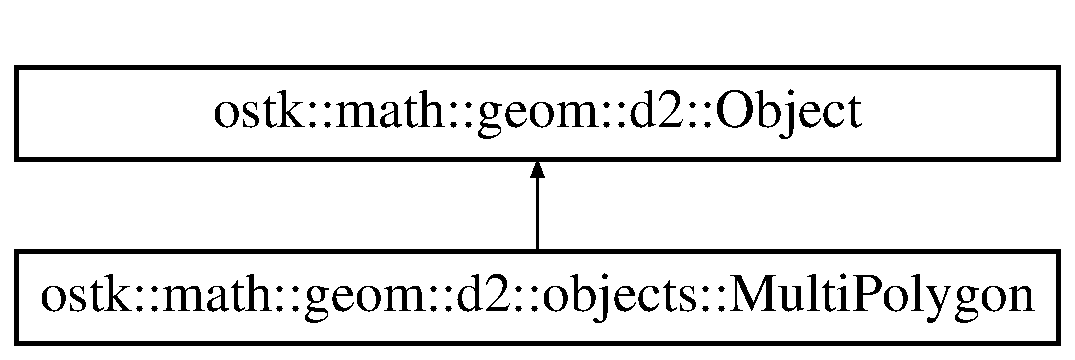
\includegraphics[height=2.000000cm]{classostk_1_1math_1_1geom_1_1d2_1_1objects_1_1_multi_polygon}
\end{center}
\end{figure}
\doxysubsection*{Public Types}
\begin{DoxyCompactItemize}
\item 
typedef Array$<$ \mbox{\hyperlink{namespaceostk_1_1math_1_1geom_1_1d2_1_1objects_a5786a3021d23f9c64937e263a2da9d27}{Polygon2d}} $>$\+::\mbox{\hyperlink{classostk_1_1math_1_1geom_1_1d2_1_1objects_1_1_multi_polygon_ade3439a576f75f37a3ebf8b4e195bad5}{Const\+Iterator}} \mbox{\hyperlink{classostk_1_1math_1_1geom_1_1d2_1_1objects_1_1_multi_polygon_ade3439a576f75f37a3ebf8b4e195bad5}{Const\+Iterator}}
\end{DoxyCompactItemize}
\doxysubsection*{Public Member Functions}
\begin{DoxyCompactItemize}
\item 
\mbox{\hyperlink{classostk_1_1math_1_1geom_1_1d2_1_1objects_1_1_multi_polygon_a70327c4d3f7f19f5ae9b32c0a715f1fd}{Multi\+Polygon}} (const Array$<$ \mbox{\hyperlink{namespaceostk_1_1math_1_1geom_1_1d2_1_1objects_a5786a3021d23f9c64937e263a2da9d27}{Polygon2d}} $>$ \&a\+Polygon\+Array=Array$<$ \mbox{\hyperlink{namespaceostk_1_1math_1_1geom_1_1d2_1_1objects_a5786a3021d23f9c64937e263a2da9d27}{Polygon2d}} $>$\+::Empty())
\begin{DoxyCompactList}\small\item\em Constructor. \end{DoxyCompactList}\item 
\mbox{\hyperlink{classostk_1_1math_1_1geom_1_1d2_1_1objects_1_1_multi_polygon_ac5b053bb605f9c24de35f0e35e3b1ee8}{Multi\+Polygon}} (const \mbox{\hyperlink{classostk_1_1math_1_1geom_1_1d2_1_1objects_1_1_multi_polygon}{Multi\+Polygon}} \&a\+Multi\+Polygon)
\begin{DoxyCompactList}\small\item\em Copy constructor. \end{DoxyCompactList}\item 
virtual \mbox{\hyperlink{classostk_1_1math_1_1geom_1_1d2_1_1objects_1_1_multi_polygon_a00964958733e630a99d445f72b9c27ba}{$\sim$\+Multi\+Polygon}} () override
\begin{DoxyCompactList}\small\item\em Destructor (virtual) \end{DoxyCompactList}\item 
\mbox{\hyperlink{classostk_1_1math_1_1geom_1_1d2_1_1objects_1_1_multi_polygon}{Multi\+Polygon}} \& \mbox{\hyperlink{classostk_1_1math_1_1geom_1_1d2_1_1objects_1_1_multi_polygon_a7864532e16a3db3ced54c09f40218af9}{operator=}} (const \mbox{\hyperlink{classostk_1_1math_1_1geom_1_1d2_1_1objects_1_1_multi_polygon}{Multi\+Polygon}} \&a\+Multi\+Polygon)
\begin{DoxyCompactList}\small\item\em Copy assignment operator. \end{DoxyCompactList}\item 
virtual \mbox{\hyperlink{classostk_1_1math_1_1geom_1_1d2_1_1objects_1_1_multi_polygon}{Multi\+Polygon}} $\ast$ \mbox{\hyperlink{classostk_1_1math_1_1geom_1_1d2_1_1objects_1_1_multi_polygon_a89fdf23e9f496c2e5f598c0dc8981c86}{clone}} () const override
\begin{DoxyCompactList}\small\item\em Clone multi-\/polygon. \end{DoxyCompactList}\item 
bool \mbox{\hyperlink{classostk_1_1math_1_1geom_1_1d2_1_1objects_1_1_multi_polygon_a8f3d731143998dacaaea1f0dffa9fa2c}{operator==}} (const \mbox{\hyperlink{classostk_1_1math_1_1geom_1_1d2_1_1objects_1_1_multi_polygon}{Multi\+Polygon}} \&a\+Multi\+Polygon) const
\begin{DoxyCompactList}\small\item\em Equal to operator. \end{DoxyCompactList}\item 
bool \mbox{\hyperlink{classostk_1_1math_1_1geom_1_1d2_1_1objects_1_1_multi_polygon_aa2c66641f9b699bdc4795d93078b8d8a}{operator!=}} (const \mbox{\hyperlink{classostk_1_1math_1_1geom_1_1d2_1_1objects_1_1_multi_polygon}{Multi\+Polygon}} \&a\+Multi\+Polygon) const
\begin{DoxyCompactList}\small\item\em Not equal to operator. \end{DoxyCompactList}\item 
virtual bool \mbox{\hyperlink{classostk_1_1math_1_1geom_1_1d2_1_1objects_1_1_multi_polygon_a27e84e80acbae4c2a7436a4d5c07b576}{is\+Defined}} () const override
\begin{DoxyCompactList}\small\item\em Check if multi-\/polygon is defined. \end{DoxyCompactList}\item 
bool \mbox{\hyperlink{classostk_1_1math_1_1geom_1_1d2_1_1objects_1_1_multi_polygon_a7b0795460707a8ee2cac31dfe7891466}{contains}} (const \mbox{\hyperlink{classostk_1_1math_1_1geom_1_1d2_1_1objects_1_1_point}{Point}} \&a\+Point) const
\begin{DoxyCompactList}\small\item\em Check if multi-\/polygon contains point. \end{DoxyCompactList}\item 
bool \mbox{\hyperlink{classostk_1_1math_1_1geom_1_1d2_1_1objects_1_1_multi_polygon_ad58e3e306864939951e8724bf9213d52}{contains}} (const \mbox{\hyperlink{classostk_1_1math_1_1geom_1_1d2_1_1objects_1_1_point_set}{Point\+Set}} \&a\+Point\+Set) const
\begin{DoxyCompactList}\small\item\em Check if multi-\/polygon contains point set. \end{DoxyCompactList}\item 
Size \mbox{\hyperlink{classostk_1_1math_1_1geom_1_1d2_1_1objects_1_1_multi_polygon_a52386a4ee9cf5fa92cb42e9d4ba3fd93}{get\+Polygon\+Count}} () const
\begin{DoxyCompactList}\small\item\em Get number of polygons. \end{DoxyCompactList}\item 
Array$<$ \mbox{\hyperlink{namespaceostk_1_1math_1_1geom_1_1d2_1_1objects_a5786a3021d23f9c64937e263a2da9d27}{Polygon2d}} $>$ \mbox{\hyperlink{classostk_1_1math_1_1geom_1_1d2_1_1objects_1_1_multi_polygon_a54cfcbcd53d46d76420ad3ff122f3ef1}{get\+Polygons}} () const
\begin{DoxyCompactList}\small\item\em Get polygons. \end{DoxyCompactList}\item 
\mbox{\hyperlink{namespaceostk_1_1math_1_1geom_1_1d2_1_1objects_a5786a3021d23f9c64937e263a2da9d27}{Polygon2d}} \mbox{\hyperlink{classostk_1_1math_1_1geom_1_1d2_1_1objects_1_1_multi_polygon_af73cf685c2fec86bbbe0aa2ee20a5e64}{get\+Convex\+Hull}} () const
\begin{DoxyCompactList}\small\item\em Get multi-\/polygon convex hull. \end{DoxyCompactList}\item 
\mbox{\hyperlink{classostk_1_1math_1_1geom_1_1d2_1_1objects_1_1_multi_polygon}{Multi\+Polygon}} \mbox{\hyperlink{classostk_1_1math_1_1geom_1_1d2_1_1objects_1_1_multi_polygon_a0762c6a4b4aaa70082394df690f3c96c}{union\+With}} (const \mbox{\hyperlink{classostk_1_1math_1_1geom_1_1d2_1_1objects_1_1_multi_polygon}{Multi\+Polygon}} \&a\+Multi\+Polygon) const
\begin{DoxyCompactList}\small\item\em Compute intersection of multi-\/polygon with multi-\/polygon. \end{DoxyCompactList}\item 
virtual String \mbox{\hyperlink{classostk_1_1math_1_1geom_1_1d2_1_1objects_1_1_multi_polygon_abf52343dc62ec2d62d971bef636f6c1c}{to\+String}} (const \mbox{\hyperlink{classostk_1_1math_1_1geom_1_1d2_1_1_object_aa76f9e30caebf4005bafbdff447f66cf}{Object\+::\+Format}} \&a\+Format=\mbox{\hyperlink{classostk_1_1math_1_1geom_1_1d2_1_1_object_aa76f9e30caebf4005bafbdff447f66cfaeb6d8ae6f20283755b339c0dc273988b}{Object\+::\+Format\+::\+Standard}}, const Integer \&a\+Precision=Integer\+::\+Undefined()) const override
\begin{DoxyCompactList}\small\item\em Get string representation. \end{DoxyCompactList}\item 
virtual void \mbox{\hyperlink{classostk_1_1math_1_1geom_1_1d2_1_1objects_1_1_multi_polygon_ab7a22decd4f9409b08e1b0e6b2bd60ef}{print}} (std\+::ostream \&an\+Output\+Stream, bool display\+Decorators=true) const override
\begin{DoxyCompactList}\small\item\em Print multi-\/polygon. \end{DoxyCompactList}\item 
\mbox{\hyperlink{classostk_1_1math_1_1geom_1_1d2_1_1objects_1_1_multi_polygon_ade3439a576f75f37a3ebf8b4e195bad5}{Multi\+Polygon\+::\+Const\+Iterator}} \mbox{\hyperlink{classostk_1_1math_1_1geom_1_1d2_1_1objects_1_1_multi_polygon_a5de8561a4153ff2565817ba6ab5ba7ca}{begin}} () const
\begin{DoxyCompactList}\small\item\em Get begin const iterator over polygons. \end{DoxyCompactList}\item 
\mbox{\hyperlink{classostk_1_1math_1_1geom_1_1d2_1_1objects_1_1_multi_polygon_ade3439a576f75f37a3ebf8b4e195bad5}{Multi\+Polygon\+::\+Const\+Iterator}} \mbox{\hyperlink{classostk_1_1math_1_1geom_1_1d2_1_1objects_1_1_multi_polygon_a05145ccf3b98e2800287a634bf98e2e6}{end}} () const
\begin{DoxyCompactList}\small\item\em Get end const iterator over polygons. \end{DoxyCompactList}\item 
virtual void \mbox{\hyperlink{classostk_1_1math_1_1geom_1_1d2_1_1objects_1_1_multi_polygon_a2dfac474c7787aac7ea0822e409bbff5}{apply\+Transformation}} (const \mbox{\hyperlink{classostk_1_1math_1_1geom_1_1d2_1_1_transformation}{Transformation}} \&a\+Transformation) override
\begin{DoxyCompactList}\small\item\em Apply transformation to multi-\/polygon. \end{DoxyCompactList}\end{DoxyCompactItemize}
\doxysubsection*{Static Public Member Functions}
\begin{DoxyCompactItemize}
\item 
static \mbox{\hyperlink{classostk_1_1math_1_1geom_1_1d2_1_1objects_1_1_multi_polygon}{Multi\+Polygon}} \mbox{\hyperlink{classostk_1_1math_1_1geom_1_1d2_1_1objects_1_1_multi_polygon_aa80a7642515417486bb846f869120fcd}{Undefined}} ()
\begin{DoxyCompactList}\small\item\em Constructs an undefined multi-\/polygon. \end{DoxyCompactList}\item 
static \mbox{\hyperlink{classostk_1_1math_1_1geom_1_1d2_1_1objects_1_1_multi_polygon}{Multi\+Polygon}} \mbox{\hyperlink{classostk_1_1math_1_1geom_1_1d2_1_1objects_1_1_multi_polygon_acbc10ee102e1a22862ec02842fff0506}{Polygon}} (const \mbox{\hyperlink{namespaceostk_1_1math_1_1geom_1_1d2_1_1objects_a5786a3021d23f9c64937e263a2da9d27}{Polygon2d}} \&a\+Polygon)
\begin{DoxyCompactList}\small\item\em Constructs a multi-\/polygon from a polygon. \end{DoxyCompactList}\end{DoxyCompactItemize}


\doxysubsection{Detailed Description}
Multi-\/polygon. 

\doxysubsection{Member Typedef Documentation}
\mbox{\Hypertarget{classostk_1_1math_1_1geom_1_1d2_1_1objects_1_1_multi_polygon_ade3439a576f75f37a3ebf8b4e195bad5}\label{classostk_1_1math_1_1geom_1_1d2_1_1objects_1_1_multi_polygon_ade3439a576f75f37a3ebf8b4e195bad5}} 
\index{ostk::math::geom::d2::objects::MultiPolygon@{ostk::math::geom::d2::objects::MultiPolygon}!ConstIterator@{ConstIterator}}
\index{ConstIterator@{ConstIterator}!ostk::math::geom::d2::objects::MultiPolygon@{ostk::math::geom::d2::objects::MultiPolygon}}
\doxysubsubsection{\texorpdfstring{ConstIterator}{ConstIterator}}
{\footnotesize\ttfamily typedef Array$<$\mbox{\hyperlink{namespaceostk_1_1math_1_1geom_1_1d2_1_1objects_a5786a3021d23f9c64937e263a2da9d27}{Polygon2d}}$>$\+::\mbox{\hyperlink{classostk_1_1math_1_1geom_1_1d2_1_1objects_1_1_multi_polygon_ade3439a576f75f37a3ebf8b4e195bad5}{Const\+Iterator}} \mbox{\hyperlink{classostk_1_1math_1_1geom_1_1d2_1_1objects_1_1_multi_polygon_ade3439a576f75f37a3ebf8b4e195bad5}{ostk\+::math\+::geom\+::d2\+::objects\+::\+Multi\+Polygon\+::\+Const\+Iterator}}}



\doxysubsection{Constructor \& Destructor Documentation}
\mbox{\Hypertarget{classostk_1_1math_1_1geom_1_1d2_1_1objects_1_1_multi_polygon_a70327c4d3f7f19f5ae9b32c0a715f1fd}\label{classostk_1_1math_1_1geom_1_1d2_1_1objects_1_1_multi_polygon_a70327c4d3f7f19f5ae9b32c0a715f1fd}} 
\index{ostk::math::geom::d2::objects::MultiPolygon@{ostk::math::geom::d2::objects::MultiPolygon}!MultiPolygon@{MultiPolygon}}
\index{MultiPolygon@{MultiPolygon}!ostk::math::geom::d2::objects::MultiPolygon@{ostk::math::geom::d2::objects::MultiPolygon}}
\doxysubsubsection{\texorpdfstring{MultiPolygon()}{MultiPolygon()}\hspace{0.1cm}{\footnotesize\ttfamily [1/2]}}
{\footnotesize\ttfamily ostk\+::math\+::geom\+::d2\+::objects\+::\+Multi\+Polygon\+::\+Multi\+Polygon (\begin{DoxyParamCaption}\item[{const Array$<$ \mbox{\hyperlink{namespaceostk_1_1math_1_1geom_1_1d2_1_1objects_a5786a3021d23f9c64937e263a2da9d27}{Polygon2d}} $>$ \&}]{a\+Polygon\+Array = {\ttfamily Array$<$\mbox{\hyperlink{namespaceostk_1_1math_1_1geom_1_1d2_1_1objects_a5786a3021d23f9c64937e263a2da9d27}{Polygon2d}}$>$\+:\+:Empty()} }\end{DoxyParamCaption})}



Constructor. 


\begin{DoxyParams}[1]{Parameters}
\mbox{\texttt{ in}}  & {\em a\+Polygon\+Array} & An array of polygons \\
\hline
\end{DoxyParams}
\mbox{\Hypertarget{classostk_1_1math_1_1geom_1_1d2_1_1objects_1_1_multi_polygon_ac5b053bb605f9c24de35f0e35e3b1ee8}\label{classostk_1_1math_1_1geom_1_1d2_1_1objects_1_1_multi_polygon_ac5b053bb605f9c24de35f0e35e3b1ee8}} 
\index{ostk::math::geom::d2::objects::MultiPolygon@{ostk::math::geom::d2::objects::MultiPolygon}!MultiPolygon@{MultiPolygon}}
\index{MultiPolygon@{MultiPolygon}!ostk::math::geom::d2::objects::MultiPolygon@{ostk::math::geom::d2::objects::MultiPolygon}}
\doxysubsubsection{\texorpdfstring{MultiPolygon()}{MultiPolygon()}\hspace{0.1cm}{\footnotesize\ttfamily [2/2]}}
{\footnotesize\ttfamily ostk\+::math\+::geom\+::d2\+::objects\+::\+Multi\+Polygon\+::\+Multi\+Polygon (\begin{DoxyParamCaption}\item[{const \mbox{\hyperlink{classostk_1_1math_1_1geom_1_1d2_1_1objects_1_1_multi_polygon}{Multi\+Polygon}} \&}]{a\+Multi\+Polygon }\end{DoxyParamCaption})}



Copy constructor. 


\begin{DoxyParams}[1]{Parameters}
\mbox{\texttt{ in}}  & {\em a\+Multi\+Polygon} & A multi-\/polygon \\
\hline
\end{DoxyParams}
\mbox{\Hypertarget{classostk_1_1math_1_1geom_1_1d2_1_1objects_1_1_multi_polygon_a00964958733e630a99d445f72b9c27ba}\label{classostk_1_1math_1_1geom_1_1d2_1_1objects_1_1_multi_polygon_a00964958733e630a99d445f72b9c27ba}} 
\index{ostk::math::geom::d2::objects::MultiPolygon@{ostk::math::geom::d2::objects::MultiPolygon}!````~MultiPolygon@{$\sim$MultiPolygon}}
\index{````~MultiPolygon@{$\sim$MultiPolygon}!ostk::math::geom::d2::objects::MultiPolygon@{ostk::math::geom::d2::objects::MultiPolygon}}
\doxysubsubsection{\texorpdfstring{$\sim$MultiPolygon()}{~MultiPolygon()}}
{\footnotesize\ttfamily ostk\+::math\+::geom\+::d2\+::objects\+::\+Multi\+Polygon\+::$\sim$\+Multi\+Polygon (\begin{DoxyParamCaption}{ }\end{DoxyParamCaption})\hspace{0.3cm}{\ttfamily [override]}, {\ttfamily [virtual]}}



Destructor (virtual) 



\doxysubsection{Member Function Documentation}
\mbox{\Hypertarget{classostk_1_1math_1_1geom_1_1d2_1_1objects_1_1_multi_polygon_a2dfac474c7787aac7ea0822e409bbff5}\label{classostk_1_1math_1_1geom_1_1d2_1_1objects_1_1_multi_polygon_a2dfac474c7787aac7ea0822e409bbff5}} 
\index{ostk::math::geom::d2::objects::MultiPolygon@{ostk::math::geom::d2::objects::MultiPolygon}!applyTransformation@{applyTransformation}}
\index{applyTransformation@{applyTransformation}!ostk::math::geom::d2::objects::MultiPolygon@{ostk::math::geom::d2::objects::MultiPolygon}}
\doxysubsubsection{\texorpdfstring{applyTransformation()}{applyTransformation()}}
{\footnotesize\ttfamily void ostk\+::math\+::geom\+::d2\+::objects\+::\+Multi\+Polygon\+::apply\+Transformation (\begin{DoxyParamCaption}\item[{const \mbox{\hyperlink{classostk_1_1math_1_1geom_1_1d2_1_1_transformation}{Transformation}} \&}]{a\+Transformation }\end{DoxyParamCaption})\hspace{0.3cm}{\ttfamily [override]}, {\ttfamily [virtual]}}



Apply transformation to multi-\/polygon. 


\begin{DoxyParams}[1]{Parameters}
\mbox{\texttt{ in}}  & {\em a\+Transformation} & A transformation \\
\hline
\end{DoxyParams}


Implements \mbox{\hyperlink{classostk_1_1math_1_1geom_1_1d2_1_1_object_a959e50211d7a680f7f904bbb752d75c9}{ostk\+::math\+::geom\+::d2\+::\+Object}}.

\mbox{\Hypertarget{classostk_1_1math_1_1geom_1_1d2_1_1objects_1_1_multi_polygon_a5de8561a4153ff2565817ba6ab5ba7ca}\label{classostk_1_1math_1_1geom_1_1d2_1_1objects_1_1_multi_polygon_a5de8561a4153ff2565817ba6ab5ba7ca}} 
\index{ostk::math::geom::d2::objects::MultiPolygon@{ostk::math::geom::d2::objects::MultiPolygon}!begin@{begin}}
\index{begin@{begin}!ostk::math::geom::d2::objects::MultiPolygon@{ostk::math::geom::d2::objects::MultiPolygon}}
\doxysubsubsection{\texorpdfstring{begin()}{begin()}}
{\footnotesize\ttfamily \mbox{\hyperlink{classostk_1_1math_1_1geom_1_1d2_1_1objects_1_1_multi_polygon_ade3439a576f75f37a3ebf8b4e195bad5}{Multi\+Polygon\+::\+Const\+Iterator}} ostk\+::math\+::geom\+::d2\+::objects\+::\+Multi\+Polygon\+::begin (\begin{DoxyParamCaption}{ }\end{DoxyParamCaption}) const}



Get begin const iterator over polygons. 

\begin{DoxyReturn}{Returns}
Const iterator 
\end{DoxyReturn}
\mbox{\Hypertarget{classostk_1_1math_1_1geom_1_1d2_1_1objects_1_1_multi_polygon_a89fdf23e9f496c2e5f598c0dc8981c86}\label{classostk_1_1math_1_1geom_1_1d2_1_1objects_1_1_multi_polygon_a89fdf23e9f496c2e5f598c0dc8981c86}} 
\index{ostk::math::geom::d2::objects::MultiPolygon@{ostk::math::geom::d2::objects::MultiPolygon}!clone@{clone}}
\index{clone@{clone}!ostk::math::geom::d2::objects::MultiPolygon@{ostk::math::geom::d2::objects::MultiPolygon}}
\doxysubsubsection{\texorpdfstring{clone()}{clone()}}
{\footnotesize\ttfamily \mbox{\hyperlink{classostk_1_1math_1_1geom_1_1d2_1_1objects_1_1_multi_polygon}{Multi\+Polygon}} $\ast$ ostk\+::math\+::geom\+::d2\+::objects\+::\+Multi\+Polygon\+::clone (\begin{DoxyParamCaption}{ }\end{DoxyParamCaption}) const\hspace{0.3cm}{\ttfamily [override]}, {\ttfamily [virtual]}}



Clone multi-\/polygon. 

\begin{DoxyReturn}{Returns}
Pointer to cloned multi-\/polygon 
\end{DoxyReturn}


Implements \mbox{\hyperlink{classostk_1_1math_1_1geom_1_1d2_1_1_object_a98dedc6792aef35308966ca768eb3e14}{ostk\+::math\+::geom\+::d2\+::\+Object}}.

\mbox{\Hypertarget{classostk_1_1math_1_1geom_1_1d2_1_1objects_1_1_multi_polygon_a7b0795460707a8ee2cac31dfe7891466}\label{classostk_1_1math_1_1geom_1_1d2_1_1objects_1_1_multi_polygon_a7b0795460707a8ee2cac31dfe7891466}} 
\index{ostk::math::geom::d2::objects::MultiPolygon@{ostk::math::geom::d2::objects::MultiPolygon}!contains@{contains}}
\index{contains@{contains}!ostk::math::geom::d2::objects::MultiPolygon@{ostk::math::geom::d2::objects::MultiPolygon}}
\doxysubsubsection{\texorpdfstring{contains()}{contains()}\hspace{0.1cm}{\footnotesize\ttfamily [1/2]}}
{\footnotesize\ttfamily bool ostk\+::math\+::geom\+::d2\+::objects\+::\+Multi\+Polygon\+::contains (\begin{DoxyParamCaption}\item[{const \mbox{\hyperlink{classostk_1_1math_1_1geom_1_1d2_1_1objects_1_1_point}{Point}} \&}]{a\+Point }\end{DoxyParamCaption}) const}



Check if multi-\/polygon contains point. 


\begin{DoxyCode}{0}
\DoxyCodeLine{\mbox{\hyperlink{classostk_1_1math_1_1geom_1_1d2_1_1objects_1_1_multi_polygon_a70327c4d3f7f19f5ae9b32c0a715f1fd}{MultiPolygon}} multiPolygon = ... ;}
\DoxyCodeLine{Point point = ... ;}
\DoxyCodeLine{multiPolygon.contains(point) ;}
\end{DoxyCode}



\begin{DoxyParams}[1]{Parameters}
\mbox{\texttt{ in}}  & {\em a\+Point} & A point \\
\hline
\end{DoxyParams}
\begin{DoxyReturn}{Returns}
True if multi-\/polygon contains point 
\end{DoxyReturn}
\mbox{\Hypertarget{classostk_1_1math_1_1geom_1_1d2_1_1objects_1_1_multi_polygon_ad58e3e306864939951e8724bf9213d52}\label{classostk_1_1math_1_1geom_1_1d2_1_1objects_1_1_multi_polygon_ad58e3e306864939951e8724bf9213d52}} 
\index{ostk::math::geom::d2::objects::MultiPolygon@{ostk::math::geom::d2::objects::MultiPolygon}!contains@{contains}}
\index{contains@{contains}!ostk::math::geom::d2::objects::MultiPolygon@{ostk::math::geom::d2::objects::MultiPolygon}}
\doxysubsubsection{\texorpdfstring{contains()}{contains()}\hspace{0.1cm}{\footnotesize\ttfamily [2/2]}}
{\footnotesize\ttfamily bool ostk\+::math\+::geom\+::d2\+::objects\+::\+Multi\+Polygon\+::contains (\begin{DoxyParamCaption}\item[{const \mbox{\hyperlink{classostk_1_1math_1_1geom_1_1d2_1_1objects_1_1_point_set}{Point\+Set}} \&}]{a\+Point\+Set }\end{DoxyParamCaption}) const}



Check if multi-\/polygon contains point set. 


\begin{DoxyCode}{0}
\DoxyCodeLine{\mbox{\hyperlink{classostk_1_1math_1_1geom_1_1d2_1_1objects_1_1_multi_polygon_a70327c4d3f7f19f5ae9b32c0a715f1fd}{MultiPolygon}} multiPolygon = ... ;}
\DoxyCodeLine{PointSet pointSet = ... ;}
\DoxyCodeLine{multiPolygon.contains(pointSet) ;}
\end{DoxyCode}



\begin{DoxyParams}[1]{Parameters}
\mbox{\texttt{ in}}  & {\em a\+Point\+Set} & A point set \\
\hline
\end{DoxyParams}
\begin{DoxyReturn}{Returns}
True if multi-\/polygon contains point set 
\end{DoxyReturn}
\mbox{\Hypertarget{classostk_1_1math_1_1geom_1_1d2_1_1objects_1_1_multi_polygon_a05145ccf3b98e2800287a634bf98e2e6}\label{classostk_1_1math_1_1geom_1_1d2_1_1objects_1_1_multi_polygon_a05145ccf3b98e2800287a634bf98e2e6}} 
\index{ostk::math::geom::d2::objects::MultiPolygon@{ostk::math::geom::d2::objects::MultiPolygon}!end@{end}}
\index{end@{end}!ostk::math::geom::d2::objects::MultiPolygon@{ostk::math::geom::d2::objects::MultiPolygon}}
\doxysubsubsection{\texorpdfstring{end()}{end()}}
{\footnotesize\ttfamily \mbox{\hyperlink{classostk_1_1math_1_1geom_1_1d2_1_1objects_1_1_multi_polygon_ade3439a576f75f37a3ebf8b4e195bad5}{Multi\+Polygon\+::\+Const\+Iterator}} ostk\+::math\+::geom\+::d2\+::objects\+::\+Multi\+Polygon\+::end (\begin{DoxyParamCaption}{ }\end{DoxyParamCaption}) const}



Get end const iterator over polygons. 

\begin{DoxyReturn}{Returns}
Const iterator 
\end{DoxyReturn}
\mbox{\Hypertarget{classostk_1_1math_1_1geom_1_1d2_1_1objects_1_1_multi_polygon_af73cf685c2fec86bbbe0aa2ee20a5e64}\label{classostk_1_1math_1_1geom_1_1d2_1_1objects_1_1_multi_polygon_af73cf685c2fec86bbbe0aa2ee20a5e64}} 
\index{ostk::math::geom::d2::objects::MultiPolygon@{ostk::math::geom::d2::objects::MultiPolygon}!getConvexHull@{getConvexHull}}
\index{getConvexHull@{getConvexHull}!ostk::math::geom::d2::objects::MultiPolygon@{ostk::math::geom::d2::objects::MultiPolygon}}
\doxysubsubsection{\texorpdfstring{getConvexHull()}{getConvexHull()}}
{\footnotesize\ttfamily \mbox{\hyperlink{namespaceostk_1_1math_1_1geom_1_1d2_1_1objects_a5786a3021d23f9c64937e263a2da9d27}{Polygon2d}} ostk\+::math\+::geom\+::d2\+::objects\+::\+Multi\+Polygon\+::get\+Convex\+Hull (\begin{DoxyParamCaption}{ }\end{DoxyParamCaption}) const}



Get multi-\/polygon convex hull. 

\begin{DoxyVerb}                https://en.wikipedia.org/wiki/Convex_hull
\end{DoxyVerb}


\begin{DoxyReturn}{Returns}
Multi-\/polygon convex hull 
\end{DoxyReturn}
\mbox{\Hypertarget{classostk_1_1math_1_1geom_1_1d2_1_1objects_1_1_multi_polygon_a52386a4ee9cf5fa92cb42e9d4ba3fd93}\label{classostk_1_1math_1_1geom_1_1d2_1_1objects_1_1_multi_polygon_a52386a4ee9cf5fa92cb42e9d4ba3fd93}} 
\index{ostk::math::geom::d2::objects::MultiPolygon@{ostk::math::geom::d2::objects::MultiPolygon}!getPolygonCount@{getPolygonCount}}
\index{getPolygonCount@{getPolygonCount}!ostk::math::geom::d2::objects::MultiPolygon@{ostk::math::geom::d2::objects::MultiPolygon}}
\doxysubsubsection{\texorpdfstring{getPolygonCount()}{getPolygonCount()}}
{\footnotesize\ttfamily Size ostk\+::math\+::geom\+::d2\+::objects\+::\+Multi\+Polygon\+::get\+Polygon\+Count (\begin{DoxyParamCaption}{ }\end{DoxyParamCaption}) const}



Get number of polygons. 

\begin{DoxyReturn}{Returns}
Number of polygons 
\end{DoxyReturn}
\mbox{\Hypertarget{classostk_1_1math_1_1geom_1_1d2_1_1objects_1_1_multi_polygon_a54cfcbcd53d46d76420ad3ff122f3ef1}\label{classostk_1_1math_1_1geom_1_1d2_1_1objects_1_1_multi_polygon_a54cfcbcd53d46d76420ad3ff122f3ef1}} 
\index{ostk::math::geom::d2::objects::MultiPolygon@{ostk::math::geom::d2::objects::MultiPolygon}!getPolygons@{getPolygons}}
\index{getPolygons@{getPolygons}!ostk::math::geom::d2::objects::MultiPolygon@{ostk::math::geom::d2::objects::MultiPolygon}}
\doxysubsubsection{\texorpdfstring{getPolygons()}{getPolygons()}}
{\footnotesize\ttfamily Array$<$ \mbox{\hyperlink{namespaceostk_1_1math_1_1geom_1_1d2_1_1objects_a5786a3021d23f9c64937e263a2da9d27}{Polygon2d}} $>$ ostk\+::math\+::geom\+::d2\+::objects\+::\+Multi\+Polygon\+::get\+Polygons (\begin{DoxyParamCaption}{ }\end{DoxyParamCaption}) const}



Get polygons. 

\begin{DoxyReturn}{Returns}
Array of polygons 
\end{DoxyReturn}
\mbox{\Hypertarget{classostk_1_1math_1_1geom_1_1d2_1_1objects_1_1_multi_polygon_a27e84e80acbae4c2a7436a4d5c07b576}\label{classostk_1_1math_1_1geom_1_1d2_1_1objects_1_1_multi_polygon_a27e84e80acbae4c2a7436a4d5c07b576}} 
\index{ostk::math::geom::d2::objects::MultiPolygon@{ostk::math::geom::d2::objects::MultiPolygon}!isDefined@{isDefined}}
\index{isDefined@{isDefined}!ostk::math::geom::d2::objects::MultiPolygon@{ostk::math::geom::d2::objects::MultiPolygon}}
\doxysubsubsection{\texorpdfstring{isDefined()}{isDefined()}}
{\footnotesize\ttfamily bool ostk\+::math\+::geom\+::d2\+::objects\+::\+Multi\+Polygon\+::is\+Defined (\begin{DoxyParamCaption}{ }\end{DoxyParamCaption}) const\hspace{0.3cm}{\ttfamily [override]}, {\ttfamily [virtual]}}



Check if multi-\/polygon is defined. 

\begin{DoxyReturn}{Returns}
True if multi-\/polygon is defined 
\end{DoxyReturn}


Implements \mbox{\hyperlink{classostk_1_1math_1_1geom_1_1d2_1_1_object_a456cc7121218d24c1322d0fe54230cc4}{ostk\+::math\+::geom\+::d2\+::\+Object}}.

\mbox{\Hypertarget{classostk_1_1math_1_1geom_1_1d2_1_1objects_1_1_multi_polygon_aa2c66641f9b699bdc4795d93078b8d8a}\label{classostk_1_1math_1_1geom_1_1d2_1_1objects_1_1_multi_polygon_aa2c66641f9b699bdc4795d93078b8d8a}} 
\index{ostk::math::geom::d2::objects::MultiPolygon@{ostk::math::geom::d2::objects::MultiPolygon}!operator"!=@{operator"!=}}
\index{operator"!=@{operator"!=}!ostk::math::geom::d2::objects::MultiPolygon@{ostk::math::geom::d2::objects::MultiPolygon}}
\doxysubsubsection{\texorpdfstring{operator"!=()}{operator!=()}}
{\footnotesize\ttfamily bool ostk\+::math\+::geom\+::d2\+::objects\+::\+Multi\+Polygon\+::operator!= (\begin{DoxyParamCaption}\item[{const \mbox{\hyperlink{classostk_1_1math_1_1geom_1_1d2_1_1objects_1_1_multi_polygon}{Multi\+Polygon}} \&}]{a\+Multi\+Polygon }\end{DoxyParamCaption}) const}



Not equal to operator. 


\begin{DoxyParams}[1]{Parameters}
\mbox{\texttt{ in}}  & {\em a\+Multi\+Polygon} & A multi-\/polygon \\
\hline
\end{DoxyParams}
\begin{DoxyReturn}{Returns}
True if multi-\/polygons are not equal 
\end{DoxyReturn}
\mbox{\Hypertarget{classostk_1_1math_1_1geom_1_1d2_1_1objects_1_1_multi_polygon_a7864532e16a3db3ced54c09f40218af9}\label{classostk_1_1math_1_1geom_1_1d2_1_1objects_1_1_multi_polygon_a7864532e16a3db3ced54c09f40218af9}} 
\index{ostk::math::geom::d2::objects::MultiPolygon@{ostk::math::geom::d2::objects::MultiPolygon}!operator=@{operator=}}
\index{operator=@{operator=}!ostk::math::geom::d2::objects::MultiPolygon@{ostk::math::geom::d2::objects::MultiPolygon}}
\doxysubsubsection{\texorpdfstring{operator=()}{operator=()}}
{\footnotesize\ttfamily \mbox{\hyperlink{classostk_1_1math_1_1geom_1_1d2_1_1objects_1_1_multi_polygon}{Multi\+Polygon}} \& ostk\+::math\+::geom\+::d2\+::objects\+::\+Multi\+Polygon\+::operator= (\begin{DoxyParamCaption}\item[{const \mbox{\hyperlink{classostk_1_1math_1_1geom_1_1d2_1_1objects_1_1_multi_polygon}{Multi\+Polygon}} \&}]{a\+Multi\+Polygon }\end{DoxyParamCaption})}



Copy assignment operator. 


\begin{DoxyParams}[1]{Parameters}
\mbox{\texttt{ in}}  & {\em a\+Multi\+Polygon} & A multi-\/polygon \\
\hline
\end{DoxyParams}
\begin{DoxyReturn}{Returns}
Reference to multi-\/polygon 
\end{DoxyReturn}
\mbox{\Hypertarget{classostk_1_1math_1_1geom_1_1d2_1_1objects_1_1_multi_polygon_a8f3d731143998dacaaea1f0dffa9fa2c}\label{classostk_1_1math_1_1geom_1_1d2_1_1objects_1_1_multi_polygon_a8f3d731143998dacaaea1f0dffa9fa2c}} 
\index{ostk::math::geom::d2::objects::MultiPolygon@{ostk::math::geom::d2::objects::MultiPolygon}!operator==@{operator==}}
\index{operator==@{operator==}!ostk::math::geom::d2::objects::MultiPolygon@{ostk::math::geom::d2::objects::MultiPolygon}}
\doxysubsubsection{\texorpdfstring{operator==()}{operator==()}}
{\footnotesize\ttfamily bool ostk\+::math\+::geom\+::d2\+::objects\+::\+Multi\+Polygon\+::operator== (\begin{DoxyParamCaption}\item[{const \mbox{\hyperlink{classostk_1_1math_1_1geom_1_1d2_1_1objects_1_1_multi_polygon}{Multi\+Polygon}} \&}]{a\+Multi\+Polygon }\end{DoxyParamCaption}) const}



Equal to operator. 


\begin{DoxyParams}[1]{Parameters}
\mbox{\texttt{ in}}  & {\em a\+Multi\+Polygon} & A multi-\/polygon \\
\hline
\end{DoxyParams}
\begin{DoxyReturn}{Returns}
True if multi-\/polygons are equal 
\end{DoxyReturn}
\mbox{\Hypertarget{classostk_1_1math_1_1geom_1_1d2_1_1objects_1_1_multi_polygon_acbc10ee102e1a22862ec02842fff0506}\label{classostk_1_1math_1_1geom_1_1d2_1_1objects_1_1_multi_polygon_acbc10ee102e1a22862ec02842fff0506}} 
\index{ostk::math::geom::d2::objects::MultiPolygon@{ostk::math::geom::d2::objects::MultiPolygon}!Polygon@{Polygon}}
\index{Polygon@{Polygon}!ostk::math::geom::d2::objects::MultiPolygon@{ostk::math::geom::d2::objects::MultiPolygon}}
\doxysubsubsection{\texorpdfstring{Polygon()}{Polygon()}}
{\footnotesize\ttfamily \mbox{\hyperlink{classostk_1_1math_1_1geom_1_1d2_1_1objects_1_1_multi_polygon}{Multi\+Polygon}} ostk\+::math\+::geom\+::d2\+::objects\+::\+Multi\+Polygon\+::\+Polygon (\begin{DoxyParamCaption}\item[{const \mbox{\hyperlink{namespaceostk_1_1math_1_1geom_1_1d2_1_1objects_a5786a3021d23f9c64937e263a2da9d27}{Polygon2d}} \&}]{a\+Polygon }\end{DoxyParamCaption})\hspace{0.3cm}{\ttfamily [static]}}



Constructs a multi-\/polygon from a polygon. 


\begin{DoxyCode}{0}
\DoxyCodeLine{\mbox{\hyperlink{classostk_1_1math_1_1geom_1_1d2_1_1objects_1_1_multi_polygon_a70327c4d3f7f19f5ae9b32c0a715f1fd}{MultiPolygon}} multiPolygon = \mbox{\hyperlink{classostk_1_1math_1_1geom_1_1d2_1_1objects_1_1_multi_polygon_acbc10ee102e1a22862ec02842fff0506}{MultiPolygon::Polygon}}(polygon) ;}
\end{DoxyCode}


\begin{DoxyReturn}{Returns}
Multi-\/polygon 
\end{DoxyReturn}
\mbox{\Hypertarget{classostk_1_1math_1_1geom_1_1d2_1_1objects_1_1_multi_polygon_ab7a22decd4f9409b08e1b0e6b2bd60ef}\label{classostk_1_1math_1_1geom_1_1d2_1_1objects_1_1_multi_polygon_ab7a22decd4f9409b08e1b0e6b2bd60ef}} 
\index{ostk::math::geom::d2::objects::MultiPolygon@{ostk::math::geom::d2::objects::MultiPolygon}!print@{print}}
\index{print@{print}!ostk::math::geom::d2::objects::MultiPolygon@{ostk::math::geom::d2::objects::MultiPolygon}}
\doxysubsubsection{\texorpdfstring{print()}{print()}}
{\footnotesize\ttfamily void ostk\+::math\+::geom\+::d2\+::objects\+::\+Multi\+Polygon\+::print (\begin{DoxyParamCaption}\item[{std\+::ostream \&}]{an\+Output\+Stream,  }\item[{bool}]{display\+Decorators = {\ttfamily true} }\end{DoxyParamCaption}) const\hspace{0.3cm}{\ttfamily [override]}, {\ttfamily [virtual]}}



Print multi-\/polygon. 


\begin{DoxyParams}[1]{Parameters}
\mbox{\texttt{ in}}  & {\em an\+Output\+Stream} & An output stream \\
\hline
\mbox{\texttt{ in}}  & {\em (optional)} & display\+Decorators If true, display decorators \\
\hline
\end{DoxyParams}


Implements \mbox{\hyperlink{classostk_1_1math_1_1geom_1_1d2_1_1_object_ae05ad883ed5a560e38f0aae7a4adc1ea}{ostk\+::math\+::geom\+::d2\+::\+Object}}.

\mbox{\Hypertarget{classostk_1_1math_1_1geom_1_1d2_1_1objects_1_1_multi_polygon_abf52343dc62ec2d62d971bef636f6c1c}\label{classostk_1_1math_1_1geom_1_1d2_1_1objects_1_1_multi_polygon_abf52343dc62ec2d62d971bef636f6c1c}} 
\index{ostk::math::geom::d2::objects::MultiPolygon@{ostk::math::geom::d2::objects::MultiPolygon}!toString@{toString}}
\index{toString@{toString}!ostk::math::geom::d2::objects::MultiPolygon@{ostk::math::geom::d2::objects::MultiPolygon}}
\doxysubsubsection{\texorpdfstring{toString()}{toString()}}
{\footnotesize\ttfamily String ostk\+::math\+::geom\+::d2\+::objects\+::\+Multi\+Polygon\+::to\+String (\begin{DoxyParamCaption}\item[{const \mbox{\hyperlink{classostk_1_1math_1_1geom_1_1d2_1_1_object_aa76f9e30caebf4005bafbdff447f66cf}{Object\+::\+Format}} \&}]{a\+Format = {\ttfamily \mbox{\hyperlink{classostk_1_1math_1_1geom_1_1d2_1_1_object_aa76f9e30caebf4005bafbdff447f66cfaeb6d8ae6f20283755b339c0dc273988b}{Object\+::\+Format\+::\+Standard}}},  }\item[{const Integer \&}]{a\+Precision = {\ttfamily Integer\+:\+:Undefined()} }\end{DoxyParamCaption}) const\hspace{0.3cm}{\ttfamily [override]}, {\ttfamily [virtual]}}



Get string representation. 


\begin{DoxyParams}[1]{Parameters}
\mbox{\texttt{ in}}  & {\em a\+Format} & A format \\
\hline
\end{DoxyParams}
\begin{DoxyReturn}{Returns}
String representation 
\end{DoxyReturn}


Implements \mbox{\hyperlink{classostk_1_1math_1_1geom_1_1d2_1_1_object_ada4c2187dd24ef02b91b6346191f677c}{ostk\+::math\+::geom\+::d2\+::\+Object}}.

\mbox{\Hypertarget{classostk_1_1math_1_1geom_1_1d2_1_1objects_1_1_multi_polygon_aa80a7642515417486bb846f869120fcd}\label{classostk_1_1math_1_1geom_1_1d2_1_1objects_1_1_multi_polygon_aa80a7642515417486bb846f869120fcd}} 
\index{ostk::math::geom::d2::objects::MultiPolygon@{ostk::math::geom::d2::objects::MultiPolygon}!Undefined@{Undefined}}
\index{Undefined@{Undefined}!ostk::math::geom::d2::objects::MultiPolygon@{ostk::math::geom::d2::objects::MultiPolygon}}
\doxysubsubsection{\texorpdfstring{Undefined()}{Undefined()}}
{\footnotesize\ttfamily \mbox{\hyperlink{classostk_1_1math_1_1geom_1_1d2_1_1objects_1_1_multi_polygon}{Multi\+Polygon}} ostk\+::math\+::geom\+::d2\+::objects\+::\+Multi\+Polygon\+::\+Undefined (\begin{DoxyParamCaption}{ }\end{DoxyParamCaption})\hspace{0.3cm}{\ttfamily [static]}}



Constructs an undefined multi-\/polygon. 


\begin{DoxyCode}{0}
\DoxyCodeLine{\mbox{\hyperlink{classostk_1_1math_1_1geom_1_1d2_1_1objects_1_1_multi_polygon_a70327c4d3f7f19f5ae9b32c0a715f1fd}{MultiPolygon}} multiPolygon = \mbox{\hyperlink{classostk_1_1math_1_1geom_1_1d2_1_1objects_1_1_multi_polygon_aa80a7642515417486bb846f869120fcd}{MultiPolygon::Undefined}}() ; \textcolor{comment}{// Undefined}}
\end{DoxyCode}


\begin{DoxyReturn}{Returns}
Undefined multi-\/polygon 
\end{DoxyReturn}
\mbox{\Hypertarget{classostk_1_1math_1_1geom_1_1d2_1_1objects_1_1_multi_polygon_a0762c6a4b4aaa70082394df690f3c96c}\label{classostk_1_1math_1_1geom_1_1d2_1_1objects_1_1_multi_polygon_a0762c6a4b4aaa70082394df690f3c96c}} 
\index{ostk::math::geom::d2::objects::MultiPolygon@{ostk::math::geom::d2::objects::MultiPolygon}!unionWith@{unionWith}}
\index{unionWith@{unionWith}!ostk::math::geom::d2::objects::MultiPolygon@{ostk::math::geom::d2::objects::MultiPolygon}}
\doxysubsubsection{\texorpdfstring{unionWith()}{unionWith()}}
{\footnotesize\ttfamily \mbox{\hyperlink{classostk_1_1math_1_1geom_1_1d2_1_1objects_1_1_multi_polygon}{Multi\+Polygon}} ostk\+::math\+::geom\+::d2\+::objects\+::\+Multi\+Polygon\+::union\+With (\begin{DoxyParamCaption}\item[{const \mbox{\hyperlink{classostk_1_1math_1_1geom_1_1d2_1_1objects_1_1_multi_polygon}{Multi\+Polygon}} \&}]{a\+Multi\+Polygon }\end{DoxyParamCaption}) const}



Compute intersection of multi-\/polygon with multi-\/polygon. 


\begin{DoxyParams}[1]{Parameters}
\mbox{\texttt{ in}}  & {\em a\+Multi\+Polygon} & A multi-\/polygon \\
\hline
\end{DoxyParams}
\begin{DoxyReturn}{Returns}
A multi-\/polygon 
\end{DoxyReturn}


The documentation for this class was generated from the following files\+:\begin{DoxyCompactItemize}
\item 
include/\+Open\+Space\+Toolkit/\+Mathematics/\+Geometry/2\+D/\+Objects/\mbox{\hyperlink{_multi_polygon_8hpp}{Multi\+Polygon.\+hpp}}\item 
src/\+Open\+Space\+Toolkit/\+Mathematics/\+Geometry/2\+D/\+Objects/\mbox{\hyperlink{_multi_polygon_8cpp}{Multi\+Polygon.\+cpp}}\end{DoxyCompactItemize}

\hypertarget{classostk_1_1math_1_1geom_1_1d2_1_1_object}{}\section{ostk\+:\+:math\+:\+:geom\+:\+:d2\+:\+:Object Class Reference}
\label{classostk_1_1math_1_1geom_1_1d2_1_1_object}\index{ostk\+::math\+::geom\+::d2\+::\+Object@{ostk\+::math\+::geom\+::d2\+::\+Object}}


2D object  




{\ttfamily \#include $<$Object.\+hpp$>$}

Inheritance diagram for ostk\+:\+:math\+:\+:geom\+:\+:d2\+:\+:Object\+:\begin{figure}[H]
\begin{center}
\leavevmode
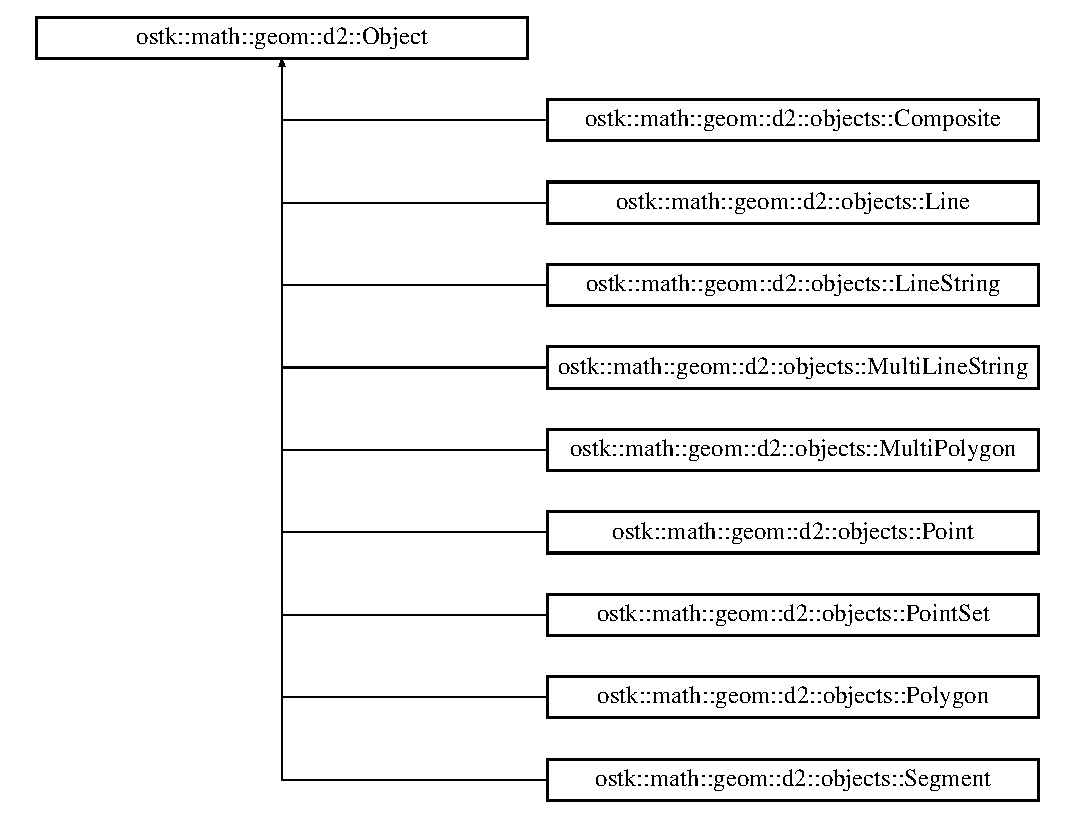
\includegraphics[height=9.000000cm]{classostk_1_1math_1_1geom_1_1d2_1_1_object}
\end{center}
\end{figure}
\subsection*{Public Types}
\begin{DoxyCompactItemize}
\item 
enum \hyperlink{classostk_1_1math_1_1geom_1_1d2_1_1_object_aa76f9e30caebf4005bafbdff447f66cf}{Format} \{ \hyperlink{classostk_1_1math_1_1geom_1_1d2_1_1_object_aa76f9e30caebf4005bafbdff447f66cfaec0fc0100c4fc1ce4eea230c3dc10360}{Format\+::\+Undefined}, 
\hyperlink{classostk_1_1math_1_1geom_1_1d2_1_1_object_aa76f9e30caebf4005bafbdff447f66cfaeb6d8ae6f20283755b339c0dc273988b}{Format\+::\+Standard}, 
\hyperlink{classostk_1_1math_1_1geom_1_1d2_1_1_object_aa76f9e30caebf4005bafbdff447f66cfa9ab05752e6beff2c783a6046ed592661}{Format\+::\+W\+KT}
 \}
\end{DoxyCompactItemize}
\subsection*{Public Member Functions}
\begin{DoxyCompactItemize}
\item 
\hyperlink{classostk_1_1math_1_1geom_1_1d2_1_1_object_a5e2d37e51e0028b18188078e13932f34}{Object} ()=default
\begin{DoxyCompactList}\small\item\em Default constructor. \end{DoxyCompactList}\item 
virtual \hyperlink{classostk_1_1math_1_1geom_1_1d2_1_1_object_a661d5d407b327b22d3139884a93eebf9}{$\sim$\+Object} ()=0
\begin{DoxyCompactList}\small\item\em Destructor (pure virtual) \end{DoxyCompactList}\item 
virtual \hyperlink{classostk_1_1math_1_1geom_1_1d2_1_1_object}{Object} $\ast$ \hyperlink{classostk_1_1math_1_1geom_1_1d2_1_1_object_a98dedc6792aef35308966ca768eb3e14}{clone} () const =0
\begin{DoxyCompactList}\small\item\em Clone object (pure virtual) \end{DoxyCompactList}\item 
bool \hyperlink{classostk_1_1math_1_1geom_1_1d2_1_1_object_aa26e3719b4b10fc5c65d047a91cf0f51}{operator==} (const \hyperlink{classostk_1_1math_1_1geom_1_1d2_1_1_object}{Object} \&an\+Object) const
\begin{DoxyCompactList}\small\item\em Not equal to operator. \end{DoxyCompactList}\item 
bool \hyperlink{classostk_1_1math_1_1geom_1_1d2_1_1_object_a10e035f09ac34d04901485d494681ff6}{operator!=} (const \hyperlink{classostk_1_1math_1_1geom_1_1d2_1_1_object}{Object} \&an\+Object) const
\begin{DoxyCompactList}\small\item\em Not equal to operator. \end{DoxyCompactList}\item 
virtual bool \hyperlink{classostk_1_1math_1_1geom_1_1d2_1_1_object_a456cc7121218d24c1322d0fe54230cc4}{is\+Defined} () const =0
\begin{DoxyCompactList}\small\item\em Check if object is defined. \end{DoxyCompactList}\item 
virtual bool \hyperlink{classostk_1_1math_1_1geom_1_1d2_1_1_object_a8791f58dd95e68a1eb4271aa15f7cd12}{intersects} (const \hyperlink{classostk_1_1math_1_1geom_1_1d2_1_1_object}{Object} \&an\+Object) const
\begin{DoxyCompactList}\small\item\em Check if object intersects another object. \end{DoxyCompactList}\item 
virtual bool \hyperlink{classostk_1_1math_1_1geom_1_1d2_1_1_object_ad932da22ca5827ee461b822fffd413c1}{contains} (const \hyperlink{classostk_1_1math_1_1geom_1_1d2_1_1_object}{Object} \&an\+Object) const
\begin{DoxyCompactList}\small\item\em Check if object contains another object. \end{DoxyCompactList}\item 
virtual String \hyperlink{classostk_1_1math_1_1geom_1_1d2_1_1_object_ada4c2187dd24ef02b91b6346191f677c}{to\+String} (const \hyperlink{classostk_1_1math_1_1geom_1_1d2_1_1_object_aa76f9e30caebf4005bafbdff447f66cf}{Object\+::\+Format} \&a\+Format=\hyperlink{classostk_1_1math_1_1geom_1_1d2_1_1_object_aa76f9e30caebf4005bafbdff447f66cfaeb6d8ae6f20283755b339c0dc273988b}{Object\+::\+Format\+::\+Standard}, const Integer \&a\+Precision=Integer\+::\+Undefined()) const =0
\begin{DoxyCompactList}\small\item\em Get string representation. \end{DoxyCompactList}\item 
virtual void \hyperlink{classostk_1_1math_1_1geom_1_1d2_1_1_object_ae05ad883ed5a560e38f0aae7a4adc1ea}{print} (std\+::ostream \&an\+Output\+Stream, bool display\+Decorators=true) const =0
\begin{DoxyCompactList}\small\item\em Print object. \end{DoxyCompactList}\item 
virtual void \hyperlink{classostk_1_1math_1_1geom_1_1d2_1_1_object_a959e50211d7a680f7f904bbb752d75c9}{apply\+Transformation} (const \hyperlink{classostk_1_1math_1_1geom_1_1d2_1_1_transformation}{Transformation} \&a\+Transformation)=0
\begin{DoxyCompactList}\small\item\em Apply transformation to object. \end{DoxyCompactList}\end{DoxyCompactItemize}
\subsection*{Friends}
\begin{DoxyCompactItemize}
\item 
std\+::ostream \& \hyperlink{classostk_1_1math_1_1geom_1_1d2_1_1_object_a418df9bf4a73078f3d494edef1743f8d}{operator$<$$<$} (std\+::ostream \&an\+Output\+Stream, const \hyperlink{classostk_1_1math_1_1geom_1_1d2_1_1_object}{Object} \&an\+Object)
\begin{DoxyCompactList}\small\item\em Output stream operator. \end{DoxyCompactList}\end{DoxyCompactItemize}


\subsection{Detailed Description}
2D object 

\subsection{Member Enumeration Documentation}
\mbox{\Hypertarget{classostk_1_1math_1_1geom_1_1d2_1_1_object_aa76f9e30caebf4005bafbdff447f66cf}\label{classostk_1_1math_1_1geom_1_1d2_1_1_object_aa76f9e30caebf4005bafbdff447f66cf}} 
\index{ostk\+::math\+::geom\+::d2\+::\+Object@{ostk\+::math\+::geom\+::d2\+::\+Object}!Format@{Format}}
\index{Format@{Format}!ostk\+::math\+::geom\+::d2\+::\+Object@{ostk\+::math\+::geom\+::d2\+::\+Object}}
\subsubsection{\texorpdfstring{Format}{Format}}
{\footnotesize\ttfamily enum \hyperlink{classostk_1_1math_1_1geom_1_1d2_1_1_object_aa76f9e30caebf4005bafbdff447f66cf}{ostk\+::math\+::geom\+::d2\+::\+Object\+::\+Format}\hspace{0.3cm}{\ttfamily [strong]}}

\begin{DoxyEnumFields}{Enumerator}
\raisebox{\heightof{T}}[0pt][0pt]{\index{Undefined@{Undefined}!ostk\+::math\+::geom\+::d2\+::\+Object@{ostk\+::math\+::geom\+::d2\+::\+Object}}\index{ostk\+::math\+::geom\+::d2\+::\+Object@{ostk\+::math\+::geom\+::d2\+::\+Object}!Undefined@{Undefined}}}\mbox{\Hypertarget{classostk_1_1math_1_1geom_1_1d2_1_1_object_aa76f9e30caebf4005bafbdff447f66cfaec0fc0100c4fc1ce4eea230c3dc10360}\label{classostk_1_1math_1_1geom_1_1d2_1_1_object_aa76f9e30caebf4005bafbdff447f66cfaec0fc0100c4fc1ce4eea230c3dc10360}} 
Undefined&Undefined format. \\
\hline

\raisebox{\heightof{T}}[0pt][0pt]{\index{Standard@{Standard}!ostk\+::math\+::geom\+::d2\+::\+Object@{ostk\+::math\+::geom\+::d2\+::\+Object}}\index{ostk\+::math\+::geom\+::d2\+::\+Object@{ostk\+::math\+::geom\+::d2\+::\+Object}!Standard@{Standard}}}\mbox{\Hypertarget{classostk_1_1math_1_1geom_1_1d2_1_1_object_aa76f9e30caebf4005bafbdff447f66cfaeb6d8ae6f20283755b339c0dc273988b}\label{classostk_1_1math_1_1geom_1_1d2_1_1_object_aa76f9e30caebf4005bafbdff447f66cfaeb6d8ae6f20283755b339c0dc273988b}} 
Standard&Standard format. \\
\hline

\raisebox{\heightof{T}}[0pt][0pt]{\index{W\+KT@{W\+KT}!ostk\+::math\+::geom\+::d2\+::\+Object@{ostk\+::math\+::geom\+::d2\+::\+Object}}\index{ostk\+::math\+::geom\+::d2\+::\+Object@{ostk\+::math\+::geom\+::d2\+::\+Object}!W\+KT@{W\+KT}}}\mbox{\Hypertarget{classostk_1_1math_1_1geom_1_1d2_1_1_object_aa76f9e30caebf4005bafbdff447f66cfa9ab05752e6beff2c783a6046ed592661}\label{classostk_1_1math_1_1geom_1_1d2_1_1_object_aa76f9e30caebf4005bafbdff447f66cfa9ab05752e6beff2c783a6046ed592661}} 
W\+KT&Well-\/\+Known Text (W\+KT) format. \\
\hline

\end{DoxyEnumFields}


\subsection{Constructor \& Destructor Documentation}
\mbox{\Hypertarget{classostk_1_1math_1_1geom_1_1d2_1_1_object_a5e2d37e51e0028b18188078e13932f34}\label{classostk_1_1math_1_1geom_1_1d2_1_1_object_a5e2d37e51e0028b18188078e13932f34}} 
\index{ostk\+::math\+::geom\+::d2\+::\+Object@{ostk\+::math\+::geom\+::d2\+::\+Object}!Object@{Object}}
\index{Object@{Object}!ostk\+::math\+::geom\+::d2\+::\+Object@{ostk\+::math\+::geom\+::d2\+::\+Object}}
\subsubsection{\texorpdfstring{Object()}{Object()}}
{\footnotesize\ttfamily ostk\+::math\+::geom\+::d2\+::\+Object\+::\+Object (\begin{DoxyParamCaption}{ }\end{DoxyParamCaption})\hspace{0.3cm}{\ttfamily [default]}}



Default constructor. 

\mbox{\Hypertarget{classostk_1_1math_1_1geom_1_1d2_1_1_object_a661d5d407b327b22d3139884a93eebf9}\label{classostk_1_1math_1_1geom_1_1d2_1_1_object_a661d5d407b327b22d3139884a93eebf9}} 
\index{ostk\+::math\+::geom\+::d2\+::\+Object@{ostk\+::math\+::geom\+::d2\+::\+Object}!````~Object@{$\sim$\+Object}}
\index{````~Object@{$\sim$\+Object}!ostk\+::math\+::geom\+::d2\+::\+Object@{ostk\+::math\+::geom\+::d2\+::\+Object}}
\subsubsection{\texorpdfstring{$\sim$\+Object()}{~Object()}}
{\footnotesize\ttfamily ostk\+::math\+::geom\+::d2\+::\+Object\+::$\sim$\+Object (\begin{DoxyParamCaption}{ }\end{DoxyParamCaption})\hspace{0.3cm}{\ttfamily [pure virtual]}}



Destructor (pure virtual) 



\subsection{Member Function Documentation}
\mbox{\Hypertarget{classostk_1_1math_1_1geom_1_1d2_1_1_object_a959e50211d7a680f7f904bbb752d75c9}\label{classostk_1_1math_1_1geom_1_1d2_1_1_object_a959e50211d7a680f7f904bbb752d75c9}} 
\index{ostk\+::math\+::geom\+::d2\+::\+Object@{ostk\+::math\+::geom\+::d2\+::\+Object}!apply\+Transformation@{apply\+Transformation}}
\index{apply\+Transformation@{apply\+Transformation}!ostk\+::math\+::geom\+::d2\+::\+Object@{ostk\+::math\+::geom\+::d2\+::\+Object}}
\subsubsection{\texorpdfstring{apply\+Transformation()}{applyTransformation()}}
{\footnotesize\ttfamily virtual void ostk\+::math\+::geom\+::d2\+::\+Object\+::apply\+Transformation (\begin{DoxyParamCaption}\item[{const \hyperlink{classostk_1_1math_1_1geom_1_1d2_1_1_transformation}{Transformation} \&}]{a\+Transformation }\end{DoxyParamCaption})\hspace{0.3cm}{\ttfamily [pure virtual]}}



Apply transformation to object. 


\begin{DoxyParams}[1]{Parameters}
\mbox{\tt in}  & {\em a\+Transformation} & A transformation \\
\hline
\end{DoxyParams}


Implemented in \hyperlink{classostk_1_1math_1_1geom_1_1d2_1_1objects_1_1_polygon_a00d04368f01daa0b234b403321453bbf}{ostk\+::math\+::geom\+::d2\+::objects\+::\+Polygon}, \hyperlink{classostk_1_1math_1_1geom_1_1d2_1_1objects_1_1_segment_afbd5fe1b8136f738a0e93b934b290394}{ostk\+::math\+::geom\+::d2\+::objects\+::\+Segment}, \hyperlink{classostk_1_1math_1_1geom_1_1d2_1_1objects_1_1_line_a75088e717153954f56cdd2df2087bdb6}{ostk\+::math\+::geom\+::d2\+::objects\+::\+Line}, \hyperlink{classostk_1_1math_1_1geom_1_1d2_1_1objects_1_1_point_set_a8c4140ca8434580a95df773d3aeed5bb}{ostk\+::math\+::geom\+::d2\+::objects\+::\+Point\+Set}, \hyperlink{classostk_1_1math_1_1geom_1_1d2_1_1objects_1_1_multi_polygon_a2dfac474c7787aac7ea0822e409bbff5}{ostk\+::math\+::geom\+::d2\+::objects\+::\+Multi\+Polygon}, \hyperlink{classostk_1_1math_1_1geom_1_1d2_1_1objects_1_1_point_aa880df23e5ee93a60dad85597c600fb0}{ostk\+::math\+::geom\+::d2\+::objects\+::\+Point}, \hyperlink{classostk_1_1math_1_1geom_1_1d2_1_1objects_1_1_line_string_afd26337c26696a0ff1b4b2e94e58f17c}{ostk\+::math\+::geom\+::d2\+::objects\+::\+Line\+String}, and \hyperlink{classostk_1_1math_1_1geom_1_1d2_1_1objects_1_1_multi_line_string_ada5fe5a183b6628831867b416901459e}{ostk\+::math\+::geom\+::d2\+::objects\+::\+Multi\+Line\+String}.

\mbox{\Hypertarget{classostk_1_1math_1_1geom_1_1d2_1_1_object_a98dedc6792aef35308966ca768eb3e14}\label{classostk_1_1math_1_1geom_1_1d2_1_1_object_a98dedc6792aef35308966ca768eb3e14}} 
\index{ostk\+::math\+::geom\+::d2\+::\+Object@{ostk\+::math\+::geom\+::d2\+::\+Object}!clone@{clone}}
\index{clone@{clone}!ostk\+::math\+::geom\+::d2\+::\+Object@{ostk\+::math\+::geom\+::d2\+::\+Object}}
\subsubsection{\texorpdfstring{clone()}{clone()}}
{\footnotesize\ttfamily virtual \hyperlink{classostk_1_1math_1_1geom_1_1d2_1_1_object}{Object}$\ast$ ostk\+::math\+::geom\+::d2\+::\+Object\+::clone (\begin{DoxyParamCaption}{ }\end{DoxyParamCaption}) const\hspace{0.3cm}{\ttfamily [pure virtual]}}



Clone object (pure virtual) 

\begin{DoxyReturn}{Returns}
Pointer to cloned object 
\end{DoxyReturn}


Implemented in \hyperlink{classostk_1_1math_1_1geom_1_1d2_1_1objects_1_1_polygon_a55e4524d1f58bf8379580e63f49f0b48}{ostk\+::math\+::geom\+::d2\+::objects\+::\+Polygon}, \hyperlink{classostk_1_1math_1_1geom_1_1d2_1_1objects_1_1_point_set_ac1d1c3727df0f10f527aa3d3551c8f4e}{ostk\+::math\+::geom\+::d2\+::objects\+::\+Point\+Set}, \hyperlink{classostk_1_1math_1_1geom_1_1d2_1_1objects_1_1_multi_polygon_a89fdf23e9f496c2e5f598c0dc8981c86}{ostk\+::math\+::geom\+::d2\+::objects\+::\+Multi\+Polygon}, \hyperlink{classostk_1_1math_1_1geom_1_1d2_1_1objects_1_1_line_string_abb5ac5e7e3e068c6597aab554e6a5e21}{ostk\+::math\+::geom\+::d2\+::objects\+::\+Line\+String}, \hyperlink{classostk_1_1math_1_1geom_1_1d2_1_1objects_1_1_segment_ad0ba7ee144638335e4f02da0de38beab}{ostk\+::math\+::geom\+::d2\+::objects\+::\+Segment}, \hyperlink{classostk_1_1math_1_1geom_1_1d2_1_1objects_1_1_multi_line_string_abf1b39f7e7f9c1f1ba9b040669863e81}{ostk\+::math\+::geom\+::d2\+::objects\+::\+Multi\+Line\+String}, \hyperlink{classostk_1_1math_1_1geom_1_1d2_1_1objects_1_1_line_a5c81c1f01b0372c7b0f8e597e77dad92}{ostk\+::math\+::geom\+::d2\+::objects\+::\+Line}, and \hyperlink{classostk_1_1math_1_1geom_1_1d2_1_1objects_1_1_point_a8550e9fe2c23c1f38e53093f4480598d}{ostk\+::math\+::geom\+::d2\+::objects\+::\+Point}.

\mbox{\Hypertarget{classostk_1_1math_1_1geom_1_1d2_1_1_object_ad932da22ca5827ee461b822fffd413c1}\label{classostk_1_1math_1_1geom_1_1d2_1_1_object_ad932da22ca5827ee461b822fffd413c1}} 
\index{ostk\+::math\+::geom\+::d2\+::\+Object@{ostk\+::math\+::geom\+::d2\+::\+Object}!contains@{contains}}
\index{contains@{contains}!ostk\+::math\+::geom\+::d2\+::\+Object@{ostk\+::math\+::geom\+::d2\+::\+Object}}
\subsubsection{\texorpdfstring{contains()}{contains()}}
{\footnotesize\ttfamily bool ostk\+::math\+::geom\+::d2\+::\+Object\+::contains (\begin{DoxyParamCaption}\item[{const \hyperlink{classostk_1_1math_1_1geom_1_1d2_1_1_object}{Object} \&}]{an\+Object }\end{DoxyParamCaption}) const\hspace{0.3cm}{\ttfamily [virtual]}}



Check if object contains another object. 


\begin{DoxyCode}
Unique<Object> objectUPtr = ... ;
Unique<Object> anotherObjectUPtr = ... ;
objectUPtr->contains(*anotherObjectUPtr) ;
\end{DoxyCode}



\begin{DoxyParams}[1]{Parameters}
\mbox{\tt in}  & {\em an\+Object} & An object \\
\hline
\end{DoxyParams}
\begin{DoxyReturn}{Returns}
True if object contains another object 
\end{DoxyReturn}
\mbox{\Hypertarget{classostk_1_1math_1_1geom_1_1d2_1_1_object_a8791f58dd95e68a1eb4271aa15f7cd12}\label{classostk_1_1math_1_1geom_1_1d2_1_1_object_a8791f58dd95e68a1eb4271aa15f7cd12}} 
\index{ostk\+::math\+::geom\+::d2\+::\+Object@{ostk\+::math\+::geom\+::d2\+::\+Object}!intersects@{intersects}}
\index{intersects@{intersects}!ostk\+::math\+::geom\+::d2\+::\+Object@{ostk\+::math\+::geom\+::d2\+::\+Object}}
\subsubsection{\texorpdfstring{intersects()}{intersects()}}
{\footnotesize\ttfamily bool ostk\+::math\+::geom\+::d2\+::\+Object\+::intersects (\begin{DoxyParamCaption}\item[{const \hyperlink{classostk_1_1math_1_1geom_1_1d2_1_1_object}{Object} \&}]{an\+Object }\end{DoxyParamCaption}) const\hspace{0.3cm}{\ttfamily [virtual]}}



Check if object intersects another object. 


\begin{DoxyCode}
Unique<Object> objectUPtr = ... ;
Unique<Object> anotherObjectUPtr = ... ;
objectUPtr->intersects(*anotherObjectUPtr) ;
\end{DoxyCode}



\begin{DoxyParams}[1]{Parameters}
\mbox{\tt in}  & {\em an\+Object} & An object \\
\hline
\end{DoxyParams}
\begin{DoxyReturn}{Returns}
True if object intersects another object 
\end{DoxyReturn}
\mbox{\Hypertarget{classostk_1_1math_1_1geom_1_1d2_1_1_object_a456cc7121218d24c1322d0fe54230cc4}\label{classostk_1_1math_1_1geom_1_1d2_1_1_object_a456cc7121218d24c1322d0fe54230cc4}} 
\index{ostk\+::math\+::geom\+::d2\+::\+Object@{ostk\+::math\+::geom\+::d2\+::\+Object}!is\+Defined@{is\+Defined}}
\index{is\+Defined@{is\+Defined}!ostk\+::math\+::geom\+::d2\+::\+Object@{ostk\+::math\+::geom\+::d2\+::\+Object}}
\subsubsection{\texorpdfstring{is\+Defined()}{isDefined()}}
{\footnotesize\ttfamily virtual bool ostk\+::math\+::geom\+::d2\+::\+Object\+::is\+Defined (\begin{DoxyParamCaption}{ }\end{DoxyParamCaption}) const\hspace{0.3cm}{\ttfamily [pure virtual]}}



Check if object is defined. 

\begin{DoxyReturn}{Returns}
True if object is defined 
\end{DoxyReturn}


Implemented in \hyperlink{classostk_1_1math_1_1geom_1_1d2_1_1objects_1_1_polygon_a81f92393dad2c6421fd4fe3834f60fa2}{ostk\+::math\+::geom\+::d2\+::objects\+::\+Polygon}, \hyperlink{classostk_1_1math_1_1geom_1_1d2_1_1objects_1_1_point_a245dd2f0268e1f162804489ac911cb0c}{ostk\+::math\+::geom\+::d2\+::objects\+::\+Point}, \hyperlink{classostk_1_1math_1_1geom_1_1d2_1_1objects_1_1_point_set_a6b2dd586eeb7f4fbf659fa9810574315}{ostk\+::math\+::geom\+::d2\+::objects\+::\+Point\+Set}, \hyperlink{classostk_1_1math_1_1geom_1_1d2_1_1objects_1_1_multi_polygon_a27e84e80acbae4c2a7436a4d5c07b576}{ostk\+::math\+::geom\+::d2\+::objects\+::\+Multi\+Polygon}, \hyperlink{classostk_1_1math_1_1geom_1_1d2_1_1objects_1_1_segment_a4e7397f14fd36b0aecd7afddd4fddf84}{ostk\+::math\+::geom\+::d2\+::objects\+::\+Segment}, \hyperlink{classostk_1_1math_1_1geom_1_1d2_1_1objects_1_1_line_a1e2a44eac16df2d9009eebf3aa85afd2}{ostk\+::math\+::geom\+::d2\+::objects\+::\+Line}, \hyperlink{classostk_1_1math_1_1geom_1_1d2_1_1objects_1_1_line_string_a0fd7edff5727e1373dbea759313313cc}{ostk\+::math\+::geom\+::d2\+::objects\+::\+Line\+String}, and \hyperlink{classostk_1_1math_1_1geom_1_1d2_1_1objects_1_1_multi_line_string_a446d9d1344336d6ec8b2ff1e46629ca2}{ostk\+::math\+::geom\+::d2\+::objects\+::\+Multi\+Line\+String}.

\mbox{\Hypertarget{classostk_1_1math_1_1geom_1_1d2_1_1_object_a10e035f09ac34d04901485d494681ff6}\label{classostk_1_1math_1_1geom_1_1d2_1_1_object_a10e035f09ac34d04901485d494681ff6}} 
\index{ostk\+::math\+::geom\+::d2\+::\+Object@{ostk\+::math\+::geom\+::d2\+::\+Object}!operator"!=@{operator"!=}}
\index{operator"!=@{operator"!=}!ostk\+::math\+::geom\+::d2\+::\+Object@{ostk\+::math\+::geom\+::d2\+::\+Object}}
\subsubsection{\texorpdfstring{operator"!=()}{operator!=()}}
{\footnotesize\ttfamily bool ostk\+::math\+::geom\+::d2\+::\+Object\+::operator!= (\begin{DoxyParamCaption}\item[{const \hyperlink{classostk_1_1math_1_1geom_1_1d2_1_1_object}{Object} \&}]{an\+Object }\end{DoxyParamCaption}) const}



Not equal to operator. 


\begin{DoxyParams}[1]{Parameters}
\mbox{\tt in}  & {\em an\+Object} & An object \\
\hline
\end{DoxyParams}
\begin{DoxyReturn}{Returns}
True if objects are not equal 
\end{DoxyReturn}
\mbox{\Hypertarget{classostk_1_1math_1_1geom_1_1d2_1_1_object_aa26e3719b4b10fc5c65d047a91cf0f51}\label{classostk_1_1math_1_1geom_1_1d2_1_1_object_aa26e3719b4b10fc5c65d047a91cf0f51}} 
\index{ostk\+::math\+::geom\+::d2\+::\+Object@{ostk\+::math\+::geom\+::d2\+::\+Object}!operator==@{operator==}}
\index{operator==@{operator==}!ostk\+::math\+::geom\+::d2\+::\+Object@{ostk\+::math\+::geom\+::d2\+::\+Object}}
\subsubsection{\texorpdfstring{operator==()}{operator==()}}
{\footnotesize\ttfamily bool ostk\+::math\+::geom\+::d2\+::\+Object\+::operator== (\begin{DoxyParamCaption}\item[{const \hyperlink{classostk_1_1math_1_1geom_1_1d2_1_1_object}{Object} \&}]{an\+Object }\end{DoxyParamCaption}) const}



Not equal to operator. 


\begin{DoxyParams}[1]{Parameters}
\mbox{\tt in}  & {\em an\+Object} & An object \\
\hline
\end{DoxyParams}
\begin{DoxyReturn}{Returns}
True if objects are equal 
\end{DoxyReturn}
\mbox{\Hypertarget{classostk_1_1math_1_1geom_1_1d2_1_1_object_ae05ad883ed5a560e38f0aae7a4adc1ea}\label{classostk_1_1math_1_1geom_1_1d2_1_1_object_ae05ad883ed5a560e38f0aae7a4adc1ea}} 
\index{ostk\+::math\+::geom\+::d2\+::\+Object@{ostk\+::math\+::geom\+::d2\+::\+Object}!print@{print}}
\index{print@{print}!ostk\+::math\+::geom\+::d2\+::\+Object@{ostk\+::math\+::geom\+::d2\+::\+Object}}
\subsubsection{\texorpdfstring{print()}{print()}}
{\footnotesize\ttfamily virtual void ostk\+::math\+::geom\+::d2\+::\+Object\+::print (\begin{DoxyParamCaption}\item[{std\+::ostream \&}]{an\+Output\+Stream,  }\item[{bool}]{display\+Decorators = {\ttfamily true} }\end{DoxyParamCaption}) const\hspace{0.3cm}{\ttfamily [pure virtual]}}



Print object. 


\begin{DoxyParams}[1]{Parameters}
\mbox{\tt in}  & {\em an\+Output\+Stream} & An output stream \\
\hline
\mbox{\tt in}  & {\em (optional)} & display\+Decorators If true, display decorators \\
\hline
\end{DoxyParams}


Implemented in \hyperlink{classostk_1_1math_1_1geom_1_1d2_1_1objects_1_1_polygon_adbf6ed9930a6dd2f3eab1c5c1b256ded}{ostk\+::math\+::geom\+::d2\+::objects\+::\+Polygon}, \hyperlink{classostk_1_1math_1_1geom_1_1d2_1_1objects_1_1_segment_a475ba5efb353218779018b9be88be276}{ostk\+::math\+::geom\+::d2\+::objects\+::\+Segment}, \hyperlink{classostk_1_1math_1_1geom_1_1d2_1_1objects_1_1_line_a8bd64cd001e4c05e3cdf7ebd7e520cb7}{ostk\+::math\+::geom\+::d2\+::objects\+::\+Line}, \hyperlink{classostk_1_1math_1_1geom_1_1d2_1_1objects_1_1_point_abcc3a265107dcccfcfe9349a6be788e5}{ostk\+::math\+::geom\+::d2\+::objects\+::\+Point}, \hyperlink{classostk_1_1math_1_1geom_1_1d2_1_1objects_1_1_point_set_aef3263b63b2e9c9667365f58faee9ac7}{ostk\+::math\+::geom\+::d2\+::objects\+::\+Point\+Set}, \hyperlink{classostk_1_1math_1_1geom_1_1d2_1_1objects_1_1_multi_polygon_ab7a22decd4f9409b08e1b0e6b2bd60ef}{ostk\+::math\+::geom\+::d2\+::objects\+::\+Multi\+Polygon}, \hyperlink{classostk_1_1math_1_1geom_1_1d2_1_1objects_1_1_line_string_afcdaa3f11f0bd830af0311392c7e9e26}{ostk\+::math\+::geom\+::d2\+::objects\+::\+Line\+String}, and \hyperlink{classostk_1_1math_1_1geom_1_1d2_1_1objects_1_1_multi_line_string_a5e90edd640ee9262194eb07d943bb8bb}{ostk\+::math\+::geom\+::d2\+::objects\+::\+Multi\+Line\+String}.

\mbox{\Hypertarget{classostk_1_1math_1_1geom_1_1d2_1_1_object_ada4c2187dd24ef02b91b6346191f677c}\label{classostk_1_1math_1_1geom_1_1d2_1_1_object_ada4c2187dd24ef02b91b6346191f677c}} 
\index{ostk\+::math\+::geom\+::d2\+::\+Object@{ostk\+::math\+::geom\+::d2\+::\+Object}!to\+String@{to\+String}}
\index{to\+String@{to\+String}!ostk\+::math\+::geom\+::d2\+::\+Object@{ostk\+::math\+::geom\+::d2\+::\+Object}}
\subsubsection{\texorpdfstring{to\+String()}{toString()}}
{\footnotesize\ttfamily virtual String ostk\+::math\+::geom\+::d2\+::\+Object\+::to\+String (\begin{DoxyParamCaption}\item[{const \hyperlink{classostk_1_1math_1_1geom_1_1d2_1_1_object_aa76f9e30caebf4005bafbdff447f66cf}{Object\+::\+Format} \&}]{a\+Format = {\ttfamily \hyperlink{classostk_1_1math_1_1geom_1_1d2_1_1_object_aa76f9e30caebf4005bafbdff447f66cfaeb6d8ae6f20283755b339c0dc273988b}{Object\+::\+Format\+::\+Standard}},  }\item[{const Integer \&}]{a\+Precision = {\ttfamily Integer\+:\+:Undefined()} }\end{DoxyParamCaption}) const\hspace{0.3cm}{\ttfamily [pure virtual]}}



Get string representation. 


\begin{DoxyParams}[1]{Parameters}
\mbox{\tt in}  & {\em a\+Format} & A format \\
\hline
\end{DoxyParams}
\begin{DoxyReturn}{Returns}
String representation 
\end{DoxyReturn}


Implemented in \hyperlink{classostk_1_1math_1_1geom_1_1d2_1_1objects_1_1_polygon_a6e672ccf5f1101de80e636f097f0a0f7}{ostk\+::math\+::geom\+::d2\+::objects\+::\+Polygon}, \hyperlink{classostk_1_1math_1_1geom_1_1d2_1_1objects_1_1_segment_ac302430065e10f1f281bb8782a904673}{ostk\+::math\+::geom\+::d2\+::objects\+::\+Segment}, \hyperlink{classostk_1_1math_1_1geom_1_1d2_1_1objects_1_1_line_a8b7e13b51e64b9db157ee08a5310646f}{ostk\+::math\+::geom\+::d2\+::objects\+::\+Line}, \hyperlink{classostk_1_1math_1_1geom_1_1d2_1_1objects_1_1_point_ac8fdaee79af60e2972257e43ff175f12}{ostk\+::math\+::geom\+::d2\+::objects\+::\+Point}, \hyperlink{classostk_1_1math_1_1geom_1_1d2_1_1objects_1_1_point_set_af032e86d9d9dcabe229a015a8361daf2}{ostk\+::math\+::geom\+::d2\+::objects\+::\+Point\+Set}, \hyperlink{classostk_1_1math_1_1geom_1_1d2_1_1objects_1_1_multi_polygon_abf52343dc62ec2d62d971bef636f6c1c}{ostk\+::math\+::geom\+::d2\+::objects\+::\+Multi\+Polygon}, \hyperlink{classostk_1_1math_1_1geom_1_1d2_1_1objects_1_1_line_string_a5312030bced48de68f8902bb6581461d}{ostk\+::math\+::geom\+::d2\+::objects\+::\+Line\+String}, and \hyperlink{classostk_1_1math_1_1geom_1_1d2_1_1objects_1_1_multi_line_string_a87df673d41e16eb2b196c8b8a852d71f}{ostk\+::math\+::geom\+::d2\+::objects\+::\+Multi\+Line\+String}.



\subsection{Friends And Related Function Documentation}
\mbox{\Hypertarget{classostk_1_1math_1_1geom_1_1d2_1_1_object_a418df9bf4a73078f3d494edef1743f8d}\label{classostk_1_1math_1_1geom_1_1d2_1_1_object_a418df9bf4a73078f3d494edef1743f8d}} 
\index{ostk\+::math\+::geom\+::d2\+::\+Object@{ostk\+::math\+::geom\+::d2\+::\+Object}!operator$<$$<$@{operator$<$$<$}}
\index{operator$<$$<$@{operator$<$$<$}!ostk\+::math\+::geom\+::d2\+::\+Object@{ostk\+::math\+::geom\+::d2\+::\+Object}}
\subsubsection{\texorpdfstring{operator$<$$<$}{operator<<}}
{\footnotesize\ttfamily std\+::ostream\& operator$<$$<$ (\begin{DoxyParamCaption}\item[{std\+::ostream \&}]{an\+Output\+Stream,  }\item[{const \hyperlink{classostk_1_1math_1_1geom_1_1d2_1_1_object}{Object} \&}]{an\+Object }\end{DoxyParamCaption})\hspace{0.3cm}{\ttfamily [friend]}}



Output stream operator. 


\begin{DoxyParams}[1]{Parameters}
\mbox{\tt in}  & {\em an\+Output\+Stream} & An output stream \\
\hline
\mbox{\tt in}  & {\em an\+Object} & An object \\
\hline
\end{DoxyParams}
\begin{DoxyReturn}{Returns}
A reference to output stream 
\end{DoxyReturn}


The documentation for this class was generated from the following files\+:\begin{DoxyCompactItemize}
\item 
include/\+Open\+Space\+Toolkit/\+Mathematics/\+Geometry/2\+D/\hyperlink{2_d_2_object_8hpp}{Object.\+hpp}\item 
src/\+Open\+Space\+Toolkit/\+Mathematics/\+Geometry/2\+D/\hyperlink{2_d_2_object_8cpp}{Object.\+cpp}\end{DoxyCompactItemize}

\hypertarget{classostk_1_1math_1_1geom_1_1d3_1_1_object}{}\section{ostk\+:\+:math\+:\+:geom\+:\+:d3\+:\+:Object Class Reference}
\label{classostk_1_1math_1_1geom_1_1d3_1_1_object}\index{ostk\+::math\+::geom\+::d3\+::\+Object@{ostk\+::math\+::geom\+::d3\+::\+Object}}


3D object  




{\ttfamily \#include $<$Object.\+hpp$>$}

Inheritance diagram for ostk\+:\+:math\+:\+:geom\+:\+:d3\+:\+:Object\+:\begin{figure}[H]
\begin{center}
\leavevmode
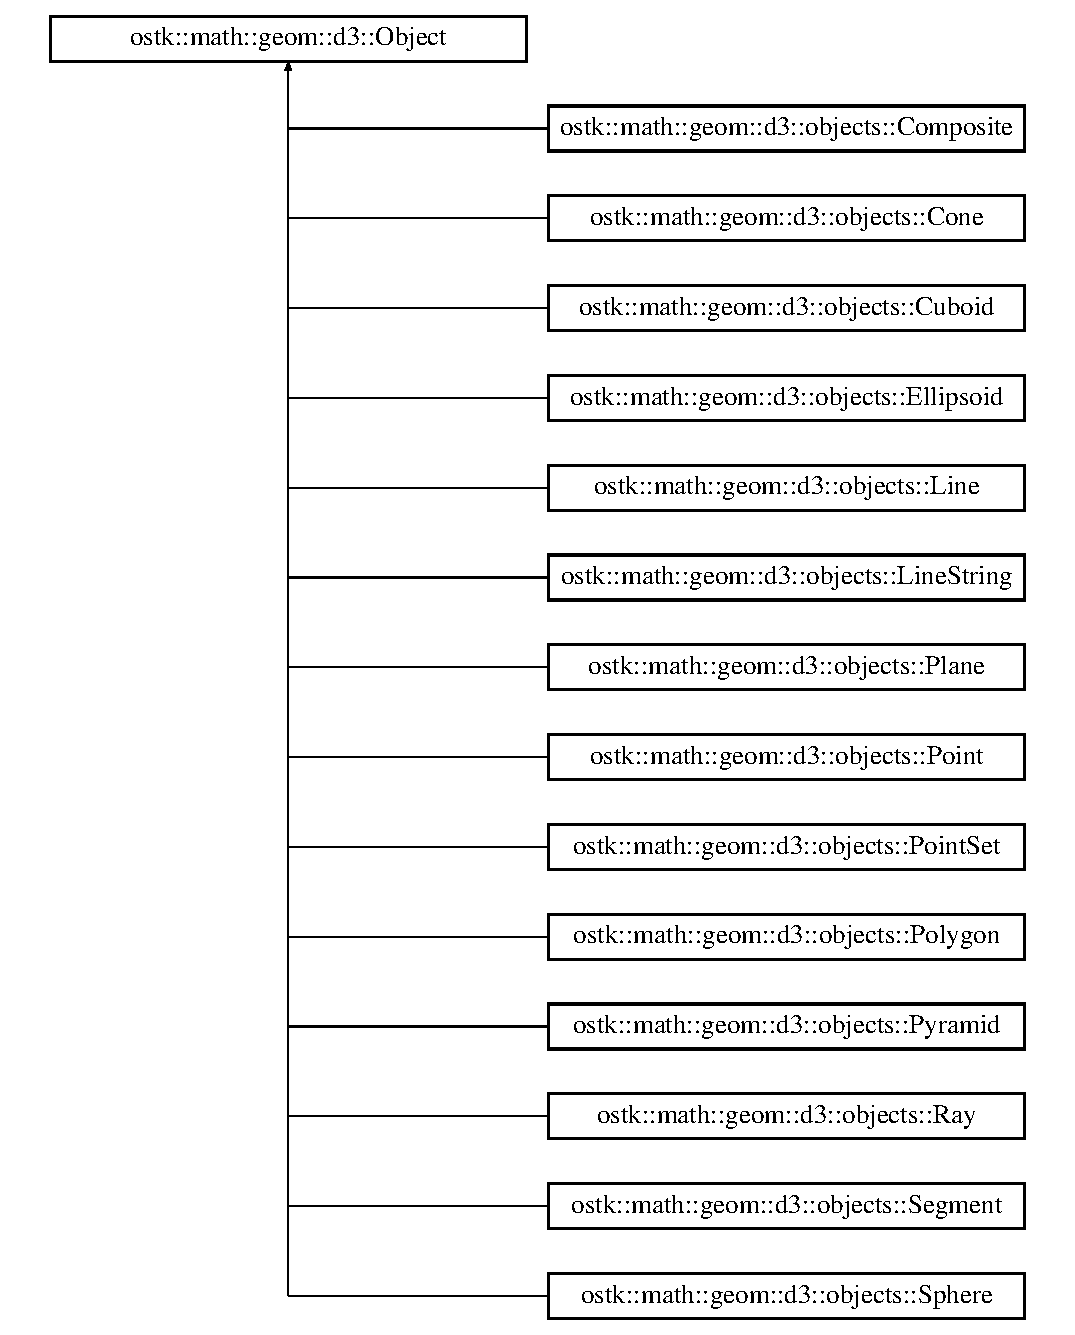
\includegraphics[height=12.000000cm]{classostk_1_1math_1_1geom_1_1d3_1_1_object}
\end{center}
\end{figure}
\subsection*{Public Member Functions}
\begin{DoxyCompactItemize}
\item 
\hyperlink{classostk_1_1math_1_1geom_1_1d3_1_1_object_ac507d37b0ef8755045938e43d20b0c94}{Object} ()=default
\begin{DoxyCompactList}\small\item\em Default constructor (default) \end{DoxyCompactList}\item 
virtual \hyperlink{classostk_1_1math_1_1geom_1_1d3_1_1_object_af626942fbad7c1ea7ba80829fdaa0e01}{$\sim$\+Object} ()=0
\begin{DoxyCompactList}\small\item\em Destructor (pure virtual) \end{DoxyCompactList}\item 
virtual \hyperlink{classostk_1_1math_1_1geom_1_1d3_1_1_object}{Object} $\ast$ \hyperlink{classostk_1_1math_1_1geom_1_1d3_1_1_object_a676013f9555f6492687f9809b2db887b}{clone} () const =0
\begin{DoxyCompactList}\small\item\em Clone object (pure virtual) \end{DoxyCompactList}\item 
bool \hyperlink{classostk_1_1math_1_1geom_1_1d3_1_1_object_a6fe8c0313e995c880062130577ea8096}{operator==} (const \hyperlink{classostk_1_1math_1_1geom_1_1d3_1_1_object}{Object} \&an\+Object) const
\begin{DoxyCompactList}\small\item\em Equal to operator. \end{DoxyCompactList}\item 
bool \hyperlink{classostk_1_1math_1_1geom_1_1d3_1_1_object_ae17716327fca875a7f63d7fb501b0529}{operator!=} (const \hyperlink{classostk_1_1math_1_1geom_1_1d3_1_1_object}{Object} \&an\+Object) const
\begin{DoxyCompactList}\small\item\em Not equal to operator. \end{DoxyCompactList}\item 
virtual bool \hyperlink{classostk_1_1math_1_1geom_1_1d3_1_1_object_a271a1964cd208be85ce9a0a429395ad8}{is\+Defined} () const =0
\begin{DoxyCompactList}\small\item\em Check if object is defined. \end{DoxyCompactList}\item 
{\footnotesize template$<$class Type $>$ }\\bool \hyperlink{classostk_1_1math_1_1geom_1_1d3_1_1_object_ab09a0b47da3dc0ca2d8170aced1ead15}{is} () const
\begin{DoxyCompactList}\small\item\em Returns true if object can be converted to type. \end{DoxyCompactList}\item 
virtual bool \hyperlink{classostk_1_1math_1_1geom_1_1d3_1_1_object_a99bfe722e7508a09a629c9eb972201e6}{intersects} (const \hyperlink{classostk_1_1math_1_1geom_1_1d3_1_1_object}{Object} \&an\+Object) const
\begin{DoxyCompactList}\small\item\em Check if object intersects another object. \end{DoxyCompactList}\item 
virtual bool \hyperlink{classostk_1_1math_1_1geom_1_1d3_1_1_object_a97edbd679b50c4663d3ab20c65cea4b9}{contains} (const \hyperlink{classostk_1_1math_1_1geom_1_1d3_1_1_object}{Object} \&an\+Object) const
\begin{DoxyCompactList}\small\item\em Check if object contains another object. \end{DoxyCompactList}\item 
{\footnotesize template$<$class Type $>$ }\\const Type \& \hyperlink{classostk_1_1math_1_1geom_1_1d3_1_1_object_ad921120c3bf1176035258fad0f654137}{as} () const
\begin{DoxyCompactList}\small\item\em Access object as its underlying type. \end{DoxyCompactList}\item 
virtual \hyperlink{classostk_1_1math_1_1geom_1_1d3_1_1_intersection}{Intersection} \hyperlink{classostk_1_1math_1_1geom_1_1d3_1_1_object_a04622921234740473c7731fa6c5bad0a}{intersection\+With} (const \hyperlink{classostk_1_1math_1_1geom_1_1d3_1_1_object}{Object} \&an\+Object) const
\begin{DoxyCompactList}\small\item\em Compute intersection of object with another object. \end{DoxyCompactList}\item 
virtual void \hyperlink{classostk_1_1math_1_1geom_1_1d3_1_1_object_ab2a2a782503b97d1cecabdfedc636fce}{print} (std\+::ostream \&an\+Output\+Stream, bool display\+Decorators=true) const =0
\begin{DoxyCompactList}\small\item\em Print object. \end{DoxyCompactList}\item 
virtual void \hyperlink{classostk_1_1math_1_1geom_1_1d3_1_1_object_ae9194dd6d2bb4df09292ffc84dccdb1d}{apply\+Transformation} (const \hyperlink{classostk_1_1math_1_1geom_1_1d3_1_1_transformation}{Transformation} \&a\+Transformation)=0
\begin{DoxyCompactList}\small\item\em Apply transformation to object. \end{DoxyCompactList}\end{DoxyCompactItemize}
\subsection*{Friends}
\begin{DoxyCompactItemize}
\item 
std\+::ostream \& \hyperlink{classostk_1_1math_1_1geom_1_1d3_1_1_object_a418df9bf4a73078f3d494edef1743f8d}{operator$<$$<$} (std\+::ostream \&an\+Output\+Stream, const \hyperlink{classostk_1_1math_1_1geom_1_1d3_1_1_object}{Object} \&an\+Object)
\begin{DoxyCompactList}\small\item\em Output stream operator. \end{DoxyCompactList}\end{DoxyCompactItemize}


\subsection{Detailed Description}
3D object 

\subsection{Constructor \& Destructor Documentation}
\mbox{\Hypertarget{classostk_1_1math_1_1geom_1_1d3_1_1_object_ac507d37b0ef8755045938e43d20b0c94}\label{classostk_1_1math_1_1geom_1_1d3_1_1_object_ac507d37b0ef8755045938e43d20b0c94}} 
\index{ostk\+::math\+::geom\+::d3\+::\+Object@{ostk\+::math\+::geom\+::d3\+::\+Object}!Object@{Object}}
\index{Object@{Object}!ostk\+::math\+::geom\+::d3\+::\+Object@{ostk\+::math\+::geom\+::d3\+::\+Object}}
\subsubsection{\texorpdfstring{Object()}{Object()}}
{\footnotesize\ttfamily ostk\+::math\+::geom\+::d3\+::\+Object\+::\+Object (\begin{DoxyParamCaption}{ }\end{DoxyParamCaption})\hspace{0.3cm}{\ttfamily [default]}}



Default constructor (default) 

\mbox{\Hypertarget{classostk_1_1math_1_1geom_1_1d3_1_1_object_af626942fbad7c1ea7ba80829fdaa0e01}\label{classostk_1_1math_1_1geom_1_1d3_1_1_object_af626942fbad7c1ea7ba80829fdaa0e01}} 
\index{ostk\+::math\+::geom\+::d3\+::\+Object@{ostk\+::math\+::geom\+::d3\+::\+Object}!````~Object@{$\sim$\+Object}}
\index{````~Object@{$\sim$\+Object}!ostk\+::math\+::geom\+::d3\+::\+Object@{ostk\+::math\+::geom\+::d3\+::\+Object}}
\subsubsection{\texorpdfstring{$\sim$\+Object()}{~Object()}}
{\footnotesize\ttfamily ostk\+::math\+::geom\+::d3\+::\+Object\+::$\sim$\+Object (\begin{DoxyParamCaption}{ }\end{DoxyParamCaption})\hspace{0.3cm}{\ttfamily [pure virtual]}}



Destructor (pure virtual) 



\subsection{Member Function Documentation}
\mbox{\Hypertarget{classostk_1_1math_1_1geom_1_1d3_1_1_object_ae9194dd6d2bb4df09292ffc84dccdb1d}\label{classostk_1_1math_1_1geom_1_1d3_1_1_object_ae9194dd6d2bb4df09292ffc84dccdb1d}} 
\index{ostk\+::math\+::geom\+::d3\+::\+Object@{ostk\+::math\+::geom\+::d3\+::\+Object}!apply\+Transformation@{apply\+Transformation}}
\index{apply\+Transformation@{apply\+Transformation}!ostk\+::math\+::geom\+::d3\+::\+Object@{ostk\+::math\+::geom\+::d3\+::\+Object}}
\subsubsection{\texorpdfstring{apply\+Transformation()}{applyTransformation()}}
{\footnotesize\ttfamily virtual void ostk\+::math\+::geom\+::d3\+::\+Object\+::apply\+Transformation (\begin{DoxyParamCaption}\item[{const \hyperlink{classostk_1_1math_1_1geom_1_1d3_1_1_transformation}{Transformation} \&}]{a\+Transformation }\end{DoxyParamCaption})\hspace{0.3cm}{\ttfamily [pure virtual]}}



Apply transformation to object. 


\begin{DoxyParams}[1]{Parameters}
\mbox{\tt in}  & {\em a\+Transformation} & A transformation \\
\hline
\end{DoxyParams}


Implemented in \hyperlink{classostk_1_1math_1_1geom_1_1d3_1_1objects_1_1_ellipsoid_aa7c60b942f6b1fa3a513bc3b549ab9e6}{ostk\+::math\+::geom\+::d3\+::objects\+::\+Ellipsoid}, \hyperlink{classostk_1_1math_1_1geom_1_1d3_1_1objects_1_1_cuboid_aaa90106ccf8120f854bdcf0f824e5610}{ostk\+::math\+::geom\+::d3\+::objects\+::\+Cuboid}, \hyperlink{classostk_1_1math_1_1geom_1_1d3_1_1objects_1_1_sphere_a421357bf4058e68e0aa636f606c6b249}{ostk\+::math\+::geom\+::d3\+::objects\+::\+Sphere}, \hyperlink{classostk_1_1math_1_1geom_1_1d3_1_1objects_1_1_plane_a4d96743e35df811f8c725561d353e245}{ostk\+::math\+::geom\+::d3\+::objects\+::\+Plane}, \hyperlink{classostk_1_1math_1_1geom_1_1d3_1_1objects_1_1_cone_a9b783e16344d65dfba68c63d1adca3e1}{ostk\+::math\+::geom\+::d3\+::objects\+::\+Cone}, \hyperlink{classostk_1_1math_1_1geom_1_1d3_1_1objects_1_1_composite_a2d99d6b4096c2f5ba3175f886e2e2c7d}{ostk\+::math\+::geom\+::d3\+::objects\+::\+Composite}, \hyperlink{classostk_1_1math_1_1geom_1_1d3_1_1objects_1_1_pyramid_ab4f31049019c0ea4b87931adf4ba7c5d}{ostk\+::math\+::geom\+::d3\+::objects\+::\+Pyramid}, \hyperlink{classostk_1_1math_1_1geom_1_1d3_1_1objects_1_1_segment_a5d2aba754d42c89224c7579944de9c4f}{ostk\+::math\+::geom\+::d3\+::objects\+::\+Segment}, \hyperlink{classostk_1_1math_1_1geom_1_1d3_1_1objects_1_1_ray_abdbc52aa6745f9d9601a8138a519d828}{ostk\+::math\+::geom\+::d3\+::objects\+::\+Ray}, \hyperlink{classostk_1_1math_1_1geom_1_1d3_1_1objects_1_1_line_ab12eb788b966601d6d09f75196a30d6f}{ostk\+::math\+::geom\+::d3\+::objects\+::\+Line}, \hyperlink{classostk_1_1math_1_1geom_1_1d3_1_1objects_1_1_polygon_abf60fe8602485822f8f07c01f6980cf5}{ostk\+::math\+::geom\+::d3\+::objects\+::\+Polygon}, \hyperlink{classostk_1_1math_1_1geom_1_1d3_1_1objects_1_1_point_a0b79a5726ac04f814b8a5b737daf0028}{ostk\+::math\+::geom\+::d3\+::objects\+::\+Point}, \hyperlink{classostk_1_1math_1_1geom_1_1d3_1_1objects_1_1_point_set_af03e071aa9d7a364a0c76f563b65a57e}{ostk\+::math\+::geom\+::d3\+::objects\+::\+Point\+Set}, and \hyperlink{classostk_1_1math_1_1geom_1_1d3_1_1objects_1_1_line_string_a8d1b47e4f9e314a5fc7df353c808dbc2}{ostk\+::math\+::geom\+::d3\+::objects\+::\+Line\+String}.

\mbox{\Hypertarget{classostk_1_1math_1_1geom_1_1d3_1_1_object_ad921120c3bf1176035258fad0f654137}\label{classostk_1_1math_1_1geom_1_1d3_1_1_object_ad921120c3bf1176035258fad0f654137}} 
\index{ostk\+::math\+::geom\+::d3\+::\+Object@{ostk\+::math\+::geom\+::d3\+::\+Object}!as@{as}}
\index{as@{as}!ostk\+::math\+::geom\+::d3\+::\+Object@{ostk\+::math\+::geom\+::d3\+::\+Object}}
\subsubsection{\texorpdfstring{as()}{as()}}
{\footnotesize\ttfamily template$<$class Type $>$ \\
const Type\& ostk\+::math\+::geom\+::d3\+::\+Object\+::as (\begin{DoxyParamCaption}{ }\end{DoxyParamCaption}) const\hspace{0.3cm}{\ttfamily [inline]}}



Access object as its underlying type. 

\begin{DoxyReturn}{Returns}
Reference to underlying type 
\end{DoxyReturn}
\mbox{\Hypertarget{classostk_1_1math_1_1geom_1_1d3_1_1_object_a676013f9555f6492687f9809b2db887b}\label{classostk_1_1math_1_1geom_1_1d3_1_1_object_a676013f9555f6492687f9809b2db887b}} 
\index{ostk\+::math\+::geom\+::d3\+::\+Object@{ostk\+::math\+::geom\+::d3\+::\+Object}!clone@{clone}}
\index{clone@{clone}!ostk\+::math\+::geom\+::d3\+::\+Object@{ostk\+::math\+::geom\+::d3\+::\+Object}}
\subsubsection{\texorpdfstring{clone()}{clone()}}
{\footnotesize\ttfamily virtual \hyperlink{classostk_1_1math_1_1geom_1_1d3_1_1_object}{Object}$\ast$ ostk\+::math\+::geom\+::d3\+::\+Object\+::clone (\begin{DoxyParamCaption}{ }\end{DoxyParamCaption}) const\hspace{0.3cm}{\ttfamily [pure virtual]}}



Clone object (pure virtual) 

\begin{DoxyReturn}{Returns}
Pointer to cloned object 
\end{DoxyReturn}


Implemented in \hyperlink{classostk_1_1math_1_1geom_1_1d3_1_1objects_1_1_point_set_a5936e0dbba4443f938d074c5e77fdac7}{ostk\+::math\+::geom\+::d3\+::objects\+::\+Point\+Set}, \hyperlink{classostk_1_1math_1_1geom_1_1d3_1_1objects_1_1_cone_a656d9720f23ab4e04bbb87dc85f9585a}{ostk\+::math\+::geom\+::d3\+::objects\+::\+Cone}, \hyperlink{classostk_1_1math_1_1geom_1_1d3_1_1objects_1_1_pyramid_aefdaacc9298ef9d9a26137b2976f7dc6}{ostk\+::math\+::geom\+::d3\+::objects\+::\+Pyramid}, \hyperlink{classostk_1_1math_1_1geom_1_1d3_1_1objects_1_1_polygon_a20f5870ed64f26d0f8e77040ececb60a}{ostk\+::math\+::geom\+::d3\+::objects\+::\+Polygon}, \hyperlink{classostk_1_1math_1_1geom_1_1d3_1_1objects_1_1_ellipsoid_a00899cd0b86395c4beef6947497bfe82}{ostk\+::math\+::geom\+::d3\+::objects\+::\+Ellipsoid}, \hyperlink{classostk_1_1math_1_1geom_1_1d3_1_1objects_1_1_cuboid_a0096ba5626ce44a892f05610f6d6eb13}{ostk\+::math\+::geom\+::d3\+::objects\+::\+Cuboid}, \hyperlink{classostk_1_1math_1_1geom_1_1d3_1_1objects_1_1_sphere_a123c8f9f89be73d95db4a0c8dd8c1c7b}{ostk\+::math\+::geom\+::d3\+::objects\+::\+Sphere}, \hyperlink{classostk_1_1math_1_1geom_1_1d3_1_1objects_1_1_composite_a3fa42c990116bf5537c943c404fa8fdd}{ostk\+::math\+::geom\+::d3\+::objects\+::\+Composite}, \hyperlink{classostk_1_1math_1_1geom_1_1d3_1_1objects_1_1_ray_aef341aa921aa184e1193c782e9198230}{ostk\+::math\+::geom\+::d3\+::objects\+::\+Ray}, \hyperlink{classostk_1_1math_1_1geom_1_1d3_1_1objects_1_1_segment_ab6d2215382c1b9fbdbd98501956d679d}{ostk\+::math\+::geom\+::d3\+::objects\+::\+Segment}, \hyperlink{classostk_1_1math_1_1geom_1_1d3_1_1objects_1_1_point_aeee85a494568471d821310dc14b5b9d5}{ostk\+::math\+::geom\+::d3\+::objects\+::\+Point}, \hyperlink{classostk_1_1math_1_1geom_1_1d3_1_1objects_1_1_line_aaf6fc08cf6b690b88c52d112052ce226}{ostk\+::math\+::geom\+::d3\+::objects\+::\+Line}, \hyperlink{classostk_1_1math_1_1geom_1_1d3_1_1objects_1_1_plane_a9db422bcf962c77b11c1d93325aebfd9}{ostk\+::math\+::geom\+::d3\+::objects\+::\+Plane}, and \hyperlink{classostk_1_1math_1_1geom_1_1d3_1_1objects_1_1_line_string_acc60289c51f32f822d7ecee85e876a75}{ostk\+::math\+::geom\+::d3\+::objects\+::\+Line\+String}.

\mbox{\Hypertarget{classostk_1_1math_1_1geom_1_1d3_1_1_object_a97edbd679b50c4663d3ab20c65cea4b9}\label{classostk_1_1math_1_1geom_1_1d3_1_1_object_a97edbd679b50c4663d3ab20c65cea4b9}} 
\index{ostk\+::math\+::geom\+::d3\+::\+Object@{ostk\+::math\+::geom\+::d3\+::\+Object}!contains@{contains}}
\index{contains@{contains}!ostk\+::math\+::geom\+::d3\+::\+Object@{ostk\+::math\+::geom\+::d3\+::\+Object}}
\subsubsection{\texorpdfstring{contains()}{contains()}}
{\footnotesize\ttfamily bool ostk\+::math\+::geom\+::d3\+::\+Object\+::contains (\begin{DoxyParamCaption}\item[{const \hyperlink{classostk_1_1math_1_1geom_1_1d3_1_1_object}{Object} \&}]{an\+Object }\end{DoxyParamCaption}) const\hspace{0.3cm}{\ttfamily [virtual]}}



Check if object contains another object. 


\begin{DoxyCode}
Unique<Object> objectUPtr = ... ;
Unique<Object> anotherObjectUPtr = ... ;
objectUPtr->contains(*anotherObjectUPtr) ;
\end{DoxyCode}



\begin{DoxyParams}[1]{Parameters}
\mbox{\tt in}  & {\em an\+Object} & An object \\
\hline
\end{DoxyParams}
\begin{DoxyReturn}{Returns}
True if object contains another object 
\end{DoxyReturn}


Reimplemented in \hyperlink{classostk_1_1math_1_1geom_1_1d3_1_1objects_1_1_composite_abe810bb7e17c444b1b556053e32750d1}{ostk\+::math\+::geom\+::d3\+::objects\+::\+Composite}.

\mbox{\Hypertarget{classostk_1_1math_1_1geom_1_1d3_1_1_object_a04622921234740473c7731fa6c5bad0a}\label{classostk_1_1math_1_1geom_1_1d3_1_1_object_a04622921234740473c7731fa6c5bad0a}} 
\index{ostk\+::math\+::geom\+::d3\+::\+Object@{ostk\+::math\+::geom\+::d3\+::\+Object}!intersection\+With@{intersection\+With}}
\index{intersection\+With@{intersection\+With}!ostk\+::math\+::geom\+::d3\+::\+Object@{ostk\+::math\+::geom\+::d3\+::\+Object}}
\subsubsection{\texorpdfstring{intersection\+With()}{intersectionWith()}}
{\footnotesize\ttfamily \hyperlink{classostk_1_1math_1_1geom_1_1d3_1_1_intersection}{Intersection} ostk\+::math\+::geom\+::d3\+::\+Object\+::intersection\+With (\begin{DoxyParamCaption}\item[{const \hyperlink{classostk_1_1math_1_1geom_1_1d3_1_1_object}{Object} \&}]{an\+Object }\end{DoxyParamCaption}) const\hspace{0.3cm}{\ttfamily [virtual]}}



Compute intersection of object with another object. 


\begin{DoxyCode}
Unique<Object> objectUPtr = ... ;
Unique<Object> anotherObjectUPtr = ... ;
Intersection intersection = objectUPtr->intersectionWith(*anotherObjectUPtr) ;
\end{DoxyCode}



\begin{DoxyParams}[1]{Parameters}
\mbox{\tt in}  & {\em an\+Object} & An object \\
\hline
\end{DoxyParams}
\begin{DoxyReturn}{Returns}
\hyperlink{classostk_1_1math_1_1geom_1_1d3_1_1_intersection}{Intersection} of object with another object 
\end{DoxyReturn}


Reimplemented in \hyperlink{classostk_1_1math_1_1geom_1_1d3_1_1objects_1_1_composite_a5c234652e274b4c2df015f89c2d3e90f}{ostk\+::math\+::geom\+::d3\+::objects\+::\+Composite}.

\mbox{\Hypertarget{classostk_1_1math_1_1geom_1_1d3_1_1_object_a99bfe722e7508a09a629c9eb972201e6}\label{classostk_1_1math_1_1geom_1_1d3_1_1_object_a99bfe722e7508a09a629c9eb972201e6}} 
\index{ostk\+::math\+::geom\+::d3\+::\+Object@{ostk\+::math\+::geom\+::d3\+::\+Object}!intersects@{intersects}}
\index{intersects@{intersects}!ostk\+::math\+::geom\+::d3\+::\+Object@{ostk\+::math\+::geom\+::d3\+::\+Object}}
\subsubsection{\texorpdfstring{intersects()}{intersects()}}
{\footnotesize\ttfamily bool ostk\+::math\+::geom\+::d3\+::\+Object\+::intersects (\begin{DoxyParamCaption}\item[{const \hyperlink{classostk_1_1math_1_1geom_1_1d3_1_1_object}{Object} \&}]{an\+Object }\end{DoxyParamCaption}) const\hspace{0.3cm}{\ttfamily [virtual]}}



Check if object intersects another object. 


\begin{DoxyCode}
Unique<Object> objectUPtr = ... ;
Unique<Object> anotherObjectUPtr = ... ;
objectUPtr->intersects(*anotherObjectUPtr) ;
\end{DoxyCode}



\begin{DoxyParams}[1]{Parameters}
\mbox{\tt in}  & {\em an\+Object} & An object \\
\hline
\end{DoxyParams}
\begin{DoxyReturn}{Returns}
True if object intersects another object 
\end{DoxyReturn}


Reimplemented in \hyperlink{classostk_1_1math_1_1geom_1_1d3_1_1objects_1_1_composite_a1064214841e9cc22475e0683fb16bce7}{ostk\+::math\+::geom\+::d3\+::objects\+::\+Composite}.

\mbox{\Hypertarget{classostk_1_1math_1_1geom_1_1d3_1_1_object_ab09a0b47da3dc0ca2d8170aced1ead15}\label{classostk_1_1math_1_1geom_1_1d3_1_1_object_ab09a0b47da3dc0ca2d8170aced1ead15}} 
\index{ostk\+::math\+::geom\+::d3\+::\+Object@{ostk\+::math\+::geom\+::d3\+::\+Object}!is@{is}}
\index{is@{is}!ostk\+::math\+::geom\+::d3\+::\+Object@{ostk\+::math\+::geom\+::d3\+::\+Object}}
\subsubsection{\texorpdfstring{is()}{is()}}
{\footnotesize\ttfamily template$<$class Type $>$ \\
bool ostk\+::math\+::geom\+::d3\+::\+Object\+::is (\begin{DoxyParamCaption}{ }\end{DoxyParamCaption}) const\hspace{0.3cm}{\ttfamily [inline]}}



Returns true if object can be converted to type. 

\begin{DoxyReturn}{Returns}
True if object can be converted to type 
\end{DoxyReturn}
\mbox{\Hypertarget{classostk_1_1math_1_1geom_1_1d3_1_1_object_a271a1964cd208be85ce9a0a429395ad8}\label{classostk_1_1math_1_1geom_1_1d3_1_1_object_a271a1964cd208be85ce9a0a429395ad8}} 
\index{ostk\+::math\+::geom\+::d3\+::\+Object@{ostk\+::math\+::geom\+::d3\+::\+Object}!is\+Defined@{is\+Defined}}
\index{is\+Defined@{is\+Defined}!ostk\+::math\+::geom\+::d3\+::\+Object@{ostk\+::math\+::geom\+::d3\+::\+Object}}
\subsubsection{\texorpdfstring{is\+Defined()}{isDefined()}}
{\footnotesize\ttfamily virtual bool ostk\+::math\+::geom\+::d3\+::\+Object\+::is\+Defined (\begin{DoxyParamCaption}{ }\end{DoxyParamCaption}) const\hspace{0.3cm}{\ttfamily [pure virtual]}}



Check if object is defined. 

\begin{DoxyReturn}{Returns}
True if object is defined 
\end{DoxyReturn}


Implemented in \hyperlink{classostk_1_1math_1_1geom_1_1d3_1_1objects_1_1_point_ad7e8b8a4f1bae1c6cd0d5895996d65b7}{ostk\+::math\+::geom\+::d3\+::objects\+::\+Point}, \hyperlink{classostk_1_1math_1_1geom_1_1d3_1_1objects_1_1_composite_afda60d7f0111f98729e9c9d96ba4e1d5}{ostk\+::math\+::geom\+::d3\+::objects\+::\+Composite}, \hyperlink{classostk_1_1math_1_1geom_1_1d3_1_1objects_1_1_ellipsoid_a21c465d185052a1631fe3ddcc131512d}{ostk\+::math\+::geom\+::d3\+::objects\+::\+Ellipsoid}, \hyperlink{classostk_1_1math_1_1geom_1_1d3_1_1objects_1_1_point_set_a2457cedb218c01b5f0b16a280ccceb95}{ostk\+::math\+::geom\+::d3\+::objects\+::\+Point\+Set}, \hyperlink{classostk_1_1math_1_1geom_1_1d3_1_1objects_1_1_cuboid_a4e7dbaf957b92cbbb02dd85c0b505366}{ostk\+::math\+::geom\+::d3\+::objects\+::\+Cuboid}, \hyperlink{classostk_1_1math_1_1geom_1_1d3_1_1objects_1_1_cone_a16491ea1637cf69ad002f59bd2b83553}{ostk\+::math\+::geom\+::d3\+::objects\+::\+Cone}, \hyperlink{classostk_1_1math_1_1geom_1_1d3_1_1objects_1_1_sphere_ab236f8c380bcc2164a5a606fdf8bc3a6}{ostk\+::math\+::geom\+::d3\+::objects\+::\+Sphere}, \hyperlink{classostk_1_1math_1_1geom_1_1d3_1_1objects_1_1_pyramid_acc4a62a7b5e51b6ad636638ca1c15504}{ostk\+::math\+::geom\+::d3\+::objects\+::\+Pyramid}, \hyperlink{classostk_1_1math_1_1geom_1_1d3_1_1objects_1_1_polygon_ae136a158ff098477abe6f8c61f37bea6}{ostk\+::math\+::geom\+::d3\+::objects\+::\+Polygon}, \hyperlink{classostk_1_1math_1_1geom_1_1d3_1_1objects_1_1_ray_ac0d991765b5d91a978fda87696b8069d}{ostk\+::math\+::geom\+::d3\+::objects\+::\+Ray}, \hyperlink{classostk_1_1math_1_1geom_1_1d3_1_1objects_1_1_segment_ab89a57a59d50bfd6fe609e92d158e6ec}{ostk\+::math\+::geom\+::d3\+::objects\+::\+Segment}, \hyperlink{classostk_1_1math_1_1geom_1_1d3_1_1objects_1_1_line_a092640b8e18d71c734185f326698f518}{ostk\+::math\+::geom\+::d3\+::objects\+::\+Line}, \hyperlink{classostk_1_1math_1_1geom_1_1d3_1_1objects_1_1_plane_a62401be167d9574a4b20f2a88f7d6c79}{ostk\+::math\+::geom\+::d3\+::objects\+::\+Plane}, and \hyperlink{classostk_1_1math_1_1geom_1_1d3_1_1objects_1_1_line_string_ae55eef3b33fb79290976d5e763ce5190}{ostk\+::math\+::geom\+::d3\+::objects\+::\+Line\+String}.

\mbox{\Hypertarget{classostk_1_1math_1_1geom_1_1d3_1_1_object_ae17716327fca875a7f63d7fb501b0529}\label{classostk_1_1math_1_1geom_1_1d3_1_1_object_ae17716327fca875a7f63d7fb501b0529}} 
\index{ostk\+::math\+::geom\+::d3\+::\+Object@{ostk\+::math\+::geom\+::d3\+::\+Object}!operator"!=@{operator"!=}}
\index{operator"!=@{operator"!=}!ostk\+::math\+::geom\+::d3\+::\+Object@{ostk\+::math\+::geom\+::d3\+::\+Object}}
\subsubsection{\texorpdfstring{operator"!=()}{operator!=()}}
{\footnotesize\ttfamily bool ostk\+::math\+::geom\+::d3\+::\+Object\+::operator!= (\begin{DoxyParamCaption}\item[{const \hyperlink{classostk_1_1math_1_1geom_1_1d3_1_1_object}{Object} \&}]{an\+Object }\end{DoxyParamCaption}) const}



Not equal to operator. 


\begin{DoxyParams}[1]{Parameters}
\mbox{\tt in}  & {\em an\+Object} & An object \\
\hline
\end{DoxyParams}
\begin{DoxyReturn}{Returns}
True if objects are not equal 
\end{DoxyReturn}
\mbox{\Hypertarget{classostk_1_1math_1_1geom_1_1d3_1_1_object_a6fe8c0313e995c880062130577ea8096}\label{classostk_1_1math_1_1geom_1_1d3_1_1_object_a6fe8c0313e995c880062130577ea8096}} 
\index{ostk\+::math\+::geom\+::d3\+::\+Object@{ostk\+::math\+::geom\+::d3\+::\+Object}!operator==@{operator==}}
\index{operator==@{operator==}!ostk\+::math\+::geom\+::d3\+::\+Object@{ostk\+::math\+::geom\+::d3\+::\+Object}}
\subsubsection{\texorpdfstring{operator==()}{operator==()}}
{\footnotesize\ttfamily bool ostk\+::math\+::geom\+::d3\+::\+Object\+::operator== (\begin{DoxyParamCaption}\item[{const \hyperlink{classostk_1_1math_1_1geom_1_1d3_1_1_object}{Object} \&}]{an\+Object }\end{DoxyParamCaption}) const}



Equal to operator. 


\begin{DoxyParams}[1]{Parameters}
\mbox{\tt in}  & {\em an\+Object} & An object \\
\hline
\end{DoxyParams}
\begin{DoxyReturn}{Returns}
True if objects are equal 
\end{DoxyReturn}
\mbox{\Hypertarget{classostk_1_1math_1_1geom_1_1d3_1_1_object_ab2a2a782503b97d1cecabdfedc636fce}\label{classostk_1_1math_1_1geom_1_1d3_1_1_object_ab2a2a782503b97d1cecabdfedc636fce}} 
\index{ostk\+::math\+::geom\+::d3\+::\+Object@{ostk\+::math\+::geom\+::d3\+::\+Object}!print@{print}}
\index{print@{print}!ostk\+::math\+::geom\+::d3\+::\+Object@{ostk\+::math\+::geom\+::d3\+::\+Object}}
\subsubsection{\texorpdfstring{print()}{print()}}
{\footnotesize\ttfamily virtual void ostk\+::math\+::geom\+::d3\+::\+Object\+::print (\begin{DoxyParamCaption}\item[{std\+::ostream \&}]{an\+Output\+Stream,  }\item[{bool}]{display\+Decorators = {\ttfamily true} }\end{DoxyParamCaption}) const\hspace{0.3cm}{\ttfamily [pure virtual]}}



Print object. 


\begin{DoxyParams}[1]{Parameters}
\mbox{\tt in}  & {\em an\+Output\+Stream} & An output stream \\
\hline
\mbox{\tt in}  & {\em (optional)} & display\+Decorators If true, display decorators \\
\hline
\end{DoxyParams}


Implemented in \hyperlink{classostk_1_1math_1_1geom_1_1d3_1_1objects_1_1_ellipsoid_a650fa20181d61ea455b98fc3330baf6e}{ostk\+::math\+::geom\+::d3\+::objects\+::\+Ellipsoid}, \hyperlink{classostk_1_1math_1_1geom_1_1d3_1_1objects_1_1_cuboid_a6ea70c4469116cc9f512e4c1a0e49016}{ostk\+::math\+::geom\+::d3\+::objects\+::\+Cuboid}, \hyperlink{classostk_1_1math_1_1geom_1_1d3_1_1objects_1_1_sphere_add7bc90c60deddcad6e3486b687a653a}{ostk\+::math\+::geom\+::d3\+::objects\+::\+Sphere}, \hyperlink{classostk_1_1math_1_1geom_1_1d3_1_1objects_1_1_plane_a312e63a716002b3bcf2954c1d30e7592}{ostk\+::math\+::geom\+::d3\+::objects\+::\+Plane}, \hyperlink{classostk_1_1math_1_1geom_1_1d3_1_1objects_1_1_cone_a511e3f582e15b11f9b571ec199fdf707}{ostk\+::math\+::geom\+::d3\+::objects\+::\+Cone}, \hyperlink{classostk_1_1math_1_1geom_1_1d3_1_1objects_1_1_composite_afa4ff037d2ab625c650ef0e45c6ea4e6}{ostk\+::math\+::geom\+::d3\+::objects\+::\+Composite}, \hyperlink{classostk_1_1math_1_1geom_1_1d3_1_1objects_1_1_pyramid_ae308eee53a721c8c41463a1ec4842a2d}{ostk\+::math\+::geom\+::d3\+::objects\+::\+Pyramid}, \hyperlink{classostk_1_1math_1_1geom_1_1d3_1_1objects_1_1_segment_a2c2029b6b84e984532f98dbd9a10ff1b}{ostk\+::math\+::geom\+::d3\+::objects\+::\+Segment}, \hyperlink{classostk_1_1math_1_1geom_1_1d3_1_1objects_1_1_ray_af2aed02d301de6d224cc757b7db573a7}{ostk\+::math\+::geom\+::d3\+::objects\+::\+Ray}, \hyperlink{classostk_1_1math_1_1geom_1_1d3_1_1objects_1_1_line_ad3e7bf31cdde2d265dd9ff644b341f2d}{ostk\+::math\+::geom\+::d3\+::objects\+::\+Line}, \hyperlink{classostk_1_1math_1_1geom_1_1d3_1_1objects_1_1_polygon_abe478a380cdd22efb082590fda923201}{ostk\+::math\+::geom\+::d3\+::objects\+::\+Polygon}, \hyperlink{classostk_1_1math_1_1geom_1_1d3_1_1objects_1_1_point_a9aa69f544cb1b2b521126c0cca39c951}{ostk\+::math\+::geom\+::d3\+::objects\+::\+Point}, \hyperlink{classostk_1_1math_1_1geom_1_1d3_1_1objects_1_1_point_set_adeeac2042e2e518b51c3b8dc4365c130}{ostk\+::math\+::geom\+::d3\+::objects\+::\+Point\+Set}, and \hyperlink{classostk_1_1math_1_1geom_1_1d3_1_1objects_1_1_line_string_a19544146cc4dc2138458c4a228e68d21}{ostk\+::math\+::geom\+::d3\+::objects\+::\+Line\+String}.



\subsection{Friends And Related Function Documentation}
\mbox{\Hypertarget{classostk_1_1math_1_1geom_1_1d3_1_1_object_a418df9bf4a73078f3d494edef1743f8d}\label{classostk_1_1math_1_1geom_1_1d3_1_1_object_a418df9bf4a73078f3d494edef1743f8d}} 
\index{ostk\+::math\+::geom\+::d3\+::\+Object@{ostk\+::math\+::geom\+::d3\+::\+Object}!operator$<$$<$@{operator$<$$<$}}
\index{operator$<$$<$@{operator$<$$<$}!ostk\+::math\+::geom\+::d3\+::\+Object@{ostk\+::math\+::geom\+::d3\+::\+Object}}
\subsubsection{\texorpdfstring{operator$<$$<$}{operator<<}}
{\footnotesize\ttfamily std\+::ostream\& operator$<$$<$ (\begin{DoxyParamCaption}\item[{std\+::ostream \&}]{an\+Output\+Stream,  }\item[{const \hyperlink{classostk_1_1math_1_1geom_1_1d3_1_1_object}{Object} \&}]{an\+Object }\end{DoxyParamCaption})\hspace{0.3cm}{\ttfamily [friend]}}



Output stream operator. 


\begin{DoxyParams}[1]{Parameters}
\mbox{\tt in}  & {\em an\+Output\+Stream} & An output stream \\
\hline
\mbox{\tt in}  & {\em an\+Object} & An object \\
\hline
\end{DoxyParams}
\begin{DoxyReturn}{Returns}
A reference to output stream 
\end{DoxyReturn}


The documentation for this class was generated from the following files\+:\begin{DoxyCompactItemize}
\item 
include/\+Open\+Space\+Toolkit/\+Mathematics/\+Geometry/3\+D/\hyperlink{3_d_2_object_8hpp}{Object.\+hpp}\item 
src/\+Open\+Space\+Toolkit/\+Mathematics/\+Geometry/3\+D/\hyperlink{3_d_2_object_8cpp}{Object.\+cpp}\end{DoxyCompactItemize}

\hypertarget{classostk_1_1math_1_1geom_1_1d3_1_1objects_1_1_plane}{}\doxysection{ostk\+::math\+::geom\+::d3\+::objects\+::Plane Class Reference}
\label{classostk_1_1math_1_1geom_1_1d3_1_1objects_1_1_plane}\index{ostk::math::geom::d3::objects::Plane@{ostk::math::geom::d3::objects::Plane}}


\mbox{\hyperlink{classostk_1_1math_1_1geom_1_1d3_1_1objects_1_1_plane}{Plane}}.  




{\ttfamily \#include $<$Plane.\+hpp$>$}

Inheritance diagram for ostk\+::math\+::geom\+::d3\+::objects\+::Plane\+:\begin{figure}[H]
\begin{center}
\leavevmode
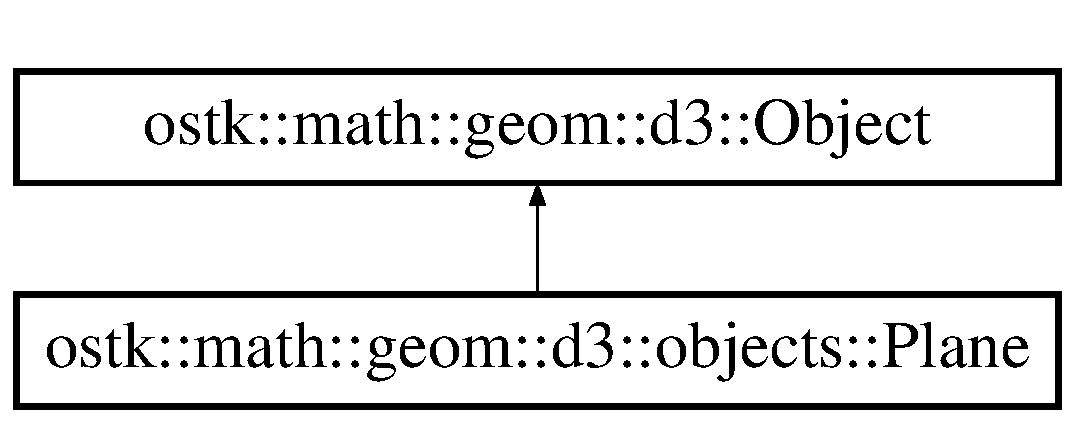
\includegraphics[height=2.000000cm]{classostk_1_1math_1_1geom_1_1d3_1_1objects_1_1_plane}
\end{center}
\end{figure}
\doxysubsection*{Public Member Functions}
\begin{DoxyCompactItemize}
\item 
\mbox{\hyperlink{classostk_1_1math_1_1geom_1_1d3_1_1objects_1_1_plane_ac66c2a3b3d9d7cd1fd507123091bb38f}{Plane}} (const \mbox{\hyperlink{classostk_1_1math_1_1geom_1_1d3_1_1objects_1_1_point}{Point}} \&a\+Point, const Vector3d \&a\+Normal\+Vector)
\begin{DoxyCompactList}\small\item\em Constructor. \end{DoxyCompactList}\item 
virtual \mbox{\hyperlink{classostk_1_1math_1_1geom_1_1d3_1_1objects_1_1_plane}{Plane}} $\ast$ \mbox{\hyperlink{classostk_1_1math_1_1geom_1_1d3_1_1objects_1_1_plane_a9db422bcf962c77b11c1d93325aebfd9}{clone}} () const override
\begin{DoxyCompactList}\small\item\em Clone plane. \end{DoxyCompactList}\item 
bool \mbox{\hyperlink{classostk_1_1math_1_1geom_1_1d3_1_1objects_1_1_plane_a93ba2703f5a835cb55e577d649b462f9}{operator==}} (const \mbox{\hyperlink{classostk_1_1math_1_1geom_1_1d3_1_1objects_1_1_plane}{Plane}} \&a\+Plane) const
\begin{DoxyCompactList}\small\item\em Equal to operator. \end{DoxyCompactList}\item 
bool \mbox{\hyperlink{classostk_1_1math_1_1geom_1_1d3_1_1objects_1_1_plane_a3e2df19f391e163bba7f7be079d19826}{operator!=}} (const \mbox{\hyperlink{classostk_1_1math_1_1geom_1_1d3_1_1objects_1_1_plane}{Plane}} \&a\+Plane) const
\begin{DoxyCompactList}\small\item\em Not equal to operator. \end{DoxyCompactList}\item 
virtual bool \mbox{\hyperlink{classostk_1_1math_1_1geom_1_1d3_1_1objects_1_1_plane_a62401be167d9574a4b20f2a88f7d6c79}{is\+Defined}} () const override
\begin{DoxyCompactList}\small\item\em Check if plane is defined. \end{DoxyCompactList}\item 
bool \mbox{\hyperlink{classostk_1_1math_1_1geom_1_1d3_1_1objects_1_1_plane_aa41d142fb1459952aef497936d351081}{intersects}} (const \mbox{\hyperlink{classostk_1_1math_1_1geom_1_1d3_1_1objects_1_1_point}{Point}} \&a\+Point) const
\begin{DoxyCompactList}\small\item\em Check if plane intersects point. \end{DoxyCompactList}\item 
bool \mbox{\hyperlink{classostk_1_1math_1_1geom_1_1d3_1_1objects_1_1_plane_a3545f1d49c58ecf570420461242e3545}{intersects}} (const \mbox{\hyperlink{classostk_1_1math_1_1geom_1_1d3_1_1objects_1_1_point_set}{Point\+Set}} \&a\+Point\+Set) const
\begin{DoxyCompactList}\small\item\em Check if plane intersects point set. \end{DoxyCompactList}\item 
bool \mbox{\hyperlink{classostk_1_1math_1_1geom_1_1d3_1_1objects_1_1_plane_a91bfde1cfff958833f3df94c70c37bcc}{intersects}} (const \mbox{\hyperlink{classostk_1_1math_1_1geom_1_1d3_1_1objects_1_1_line}{Line}} \&a\+Line) const
\begin{DoxyCompactList}\small\item\em Check if plane intersects line. \end{DoxyCompactList}\item 
bool \mbox{\hyperlink{classostk_1_1math_1_1geom_1_1d3_1_1objects_1_1_plane_af1e179dece2fbba1482fdd9a98fc58ea}{intersects}} (const \mbox{\hyperlink{classostk_1_1math_1_1geom_1_1d3_1_1objects_1_1_ray}{Ray}} \&a\+Ray) const
\begin{DoxyCompactList}\small\item\em Check if plane intersects ray. \end{DoxyCompactList}\item 
bool \mbox{\hyperlink{classostk_1_1math_1_1geom_1_1d3_1_1objects_1_1_plane_a7b1d164ebd925ed9329479f9f522c7f9}{intersects}} (const \mbox{\hyperlink{classostk_1_1math_1_1geom_1_1d3_1_1objects_1_1_segment}{Segment}} \&a\+Segment) const
\begin{DoxyCompactList}\small\item\em Check if plane intersects segment. \end{DoxyCompactList}\item 
bool \mbox{\hyperlink{classostk_1_1math_1_1geom_1_1d3_1_1objects_1_1_plane_a62deb80d18f6c9c86a5765a20e91d490}{contains}} (const \mbox{\hyperlink{classostk_1_1math_1_1geom_1_1d3_1_1objects_1_1_point}{Point}} \&a\+Point) const
\begin{DoxyCompactList}\small\item\em Check if plane contains point. \end{DoxyCompactList}\item 
bool \mbox{\hyperlink{classostk_1_1math_1_1geom_1_1d3_1_1objects_1_1_plane_a5113cf47ca5ef948fa8f43074291108d}{contains}} (const \mbox{\hyperlink{classostk_1_1math_1_1geom_1_1d3_1_1objects_1_1_point_set}{Point\+Set}} \&a\+Point\+Set) const
\begin{DoxyCompactList}\small\item\em Check if plane contains point set. \end{DoxyCompactList}\item 
bool \mbox{\hyperlink{classostk_1_1math_1_1geom_1_1d3_1_1objects_1_1_plane_ad3cc8cc87bd61e8804bc4e207c662e5c}{contains}} (const \mbox{\hyperlink{classostk_1_1math_1_1geom_1_1d3_1_1objects_1_1_line}{Line}} \&a\+Line) const
\begin{DoxyCompactList}\small\item\em Check if plane contains line. \end{DoxyCompactList}\item 
bool \mbox{\hyperlink{classostk_1_1math_1_1geom_1_1d3_1_1objects_1_1_plane_a71b173f52939462f312dd0885931ca6a}{contains}} (const \mbox{\hyperlink{classostk_1_1math_1_1geom_1_1d3_1_1objects_1_1_ray}{Ray}} \&a\+Ray) const
\begin{DoxyCompactList}\small\item\em Check if plane contains ray. \end{DoxyCompactList}\item 
bool \mbox{\hyperlink{classostk_1_1math_1_1geom_1_1d3_1_1objects_1_1_plane_a229e30b431a2a2b8d00c02dbfba83e91}{contains}} (const \mbox{\hyperlink{classostk_1_1math_1_1geom_1_1d3_1_1objects_1_1_segment}{Segment}} \&a\+Segment) const
\begin{DoxyCompactList}\small\item\em Check if plane contains segment. \end{DoxyCompactList}\item 
\mbox{\hyperlink{classostk_1_1math_1_1geom_1_1d3_1_1objects_1_1_point}{Point}} \mbox{\hyperlink{classostk_1_1math_1_1geom_1_1d3_1_1objects_1_1_plane_a9e8b046781fec60f76faac94869908ec}{get\+Point}} () const
\begin{DoxyCompactList}\small\item\em Get plane point. \end{DoxyCompactList}\item 
Vector3d \mbox{\hyperlink{classostk_1_1math_1_1geom_1_1d3_1_1objects_1_1_plane_adad78a414d67a13cd87c9f5c569990ea}{get\+Normal\+Vector}} () const
\begin{DoxyCompactList}\small\item\em Get plane normal vector. \end{DoxyCompactList}\item 
\mbox{\hyperlink{classostk_1_1math_1_1geom_1_1d3_1_1_intersection}{Intersection}} \mbox{\hyperlink{classostk_1_1math_1_1geom_1_1d3_1_1objects_1_1_plane_a1b0b693ea9fbe937dbaf39eda6fe86e6}{intersection\+With}} (const \mbox{\hyperlink{classostk_1_1math_1_1geom_1_1d3_1_1objects_1_1_point}{Point}} \&a\+Point) const
\begin{DoxyCompactList}\small\item\em Compute intersection of plane with point. \end{DoxyCompactList}\item 
\mbox{\hyperlink{classostk_1_1math_1_1geom_1_1d3_1_1_intersection}{Intersection}} \mbox{\hyperlink{classostk_1_1math_1_1geom_1_1d3_1_1objects_1_1_plane_a6fa36d3b2dda5f7a3e2774a4c35006b5}{intersection\+With}} (const \mbox{\hyperlink{classostk_1_1math_1_1geom_1_1d3_1_1objects_1_1_point_set}{Point\+Set}} \&a\+Point\+Set) const
\begin{DoxyCompactList}\small\item\em Compute intersection of plane with point set. \end{DoxyCompactList}\item 
\mbox{\hyperlink{classostk_1_1math_1_1geom_1_1d3_1_1_intersection}{Intersection}} \mbox{\hyperlink{classostk_1_1math_1_1geom_1_1d3_1_1objects_1_1_plane_aa85ba34c3f94fabf1e632f98fea48115}{intersection\+With}} (const \mbox{\hyperlink{classostk_1_1math_1_1geom_1_1d3_1_1objects_1_1_line}{Line}} \&a\+Line) const
\begin{DoxyCompactList}\small\item\em Compute intersection of plane with line. \end{DoxyCompactList}\item 
\mbox{\hyperlink{classostk_1_1math_1_1geom_1_1d3_1_1_intersection}{Intersection}} \mbox{\hyperlink{classostk_1_1math_1_1geom_1_1d3_1_1objects_1_1_plane_aa7a3428e047dee047890f82893abd8d7}{intersection\+With}} (const \mbox{\hyperlink{classostk_1_1math_1_1geom_1_1d3_1_1objects_1_1_ray}{Ray}} \&a\+Ray) const
\begin{DoxyCompactList}\small\item\em Compute intersection of plane with ray. \end{DoxyCompactList}\item 
\mbox{\hyperlink{classostk_1_1math_1_1geom_1_1d3_1_1_intersection}{Intersection}} \mbox{\hyperlink{classostk_1_1math_1_1geom_1_1d3_1_1objects_1_1_plane_a0c76a99ec76e6f1dc5fc5b39737b282e}{intersection\+With}} (const \mbox{\hyperlink{classostk_1_1math_1_1geom_1_1d3_1_1objects_1_1_segment}{Segment}} \&a\+Segment) const
\begin{DoxyCompactList}\small\item\em Compute intersection of plane with segment. \end{DoxyCompactList}\item 
virtual void \mbox{\hyperlink{classostk_1_1math_1_1geom_1_1d3_1_1objects_1_1_plane_a312e63a716002b3bcf2954c1d30e7592}{print}} (std\+::ostream \&an\+Output\+Stream, bool display\+Decorators=true) const override
\begin{DoxyCompactList}\small\item\em Print plane. \end{DoxyCompactList}\item 
virtual void \mbox{\hyperlink{classostk_1_1math_1_1geom_1_1d3_1_1objects_1_1_plane_a4d96743e35df811f8c725561d353e245}{apply\+Transformation}} (const \mbox{\hyperlink{classostk_1_1math_1_1geom_1_1d3_1_1_transformation}{Transformation}} \&a\+Transformation) override
\begin{DoxyCompactList}\small\item\em Apply transformation to plane. \end{DoxyCompactList}\end{DoxyCompactItemize}
\doxysubsection*{Static Public Member Functions}
\begin{DoxyCompactItemize}
\item 
static \mbox{\hyperlink{classostk_1_1math_1_1geom_1_1d3_1_1objects_1_1_plane}{Plane}} \mbox{\hyperlink{classostk_1_1math_1_1geom_1_1d3_1_1objects_1_1_plane_a162297dffbd860cd6c383e412708734f}{Undefined}} ()
\begin{DoxyCompactList}\small\item\em Constructs an undefined plane. \end{DoxyCompactList}\end{DoxyCompactItemize}


\doxysubsection{Detailed Description}
\mbox{\hyperlink{classostk_1_1math_1_1geom_1_1d3_1_1objects_1_1_plane}{Plane}}. 

\begin{DoxyVerb}                        A plane is a flat, two-dimensional surface that extends infinitely far.
\end{DoxyVerb}


\href{https://en.wikipedia.org/wiki/Plane_}{\texttt{ https\+://en.\+wikipedia.\+org/wiki/\+Plane\+\_\+}}(geometry) 

\doxysubsection{Constructor \& Destructor Documentation}
\mbox{\Hypertarget{classostk_1_1math_1_1geom_1_1d3_1_1objects_1_1_plane_ac66c2a3b3d9d7cd1fd507123091bb38f}\label{classostk_1_1math_1_1geom_1_1d3_1_1objects_1_1_plane_ac66c2a3b3d9d7cd1fd507123091bb38f}} 
\index{ostk::math::geom::d3::objects::Plane@{ostk::math::geom::d3::objects::Plane}!Plane@{Plane}}
\index{Plane@{Plane}!ostk::math::geom::d3::objects::Plane@{ostk::math::geom::d3::objects::Plane}}
\doxysubsubsection{\texorpdfstring{Plane()}{Plane()}}
{\footnotesize\ttfamily ostk\+::math\+::geom\+::d3\+::objects\+::\+Plane\+::\+Plane (\begin{DoxyParamCaption}\item[{const \mbox{\hyperlink{classostk_1_1math_1_1geom_1_1d3_1_1objects_1_1_point}{Point}} \&}]{a\+Point,  }\item[{const Vector3d \&}]{a\+Normal\+Vector }\end{DoxyParamCaption})}



Constructor. 


\begin{DoxyCode}{0}
\DoxyCodeLine{\mbox{\hyperlink{classostk_1_1math_1_1geom_1_1d3_1_1objects_1_1_plane_ac66c2a3b3d9d7cd1fd507123091bb38f}{Plane}} plane(\{ 0.0, 0.0, 0.0 \}, \{ 0.0, 0.0, 1.0 \}) ;}
\end{DoxyCode}



\begin{DoxyParams}[1]{Parameters}
\mbox{\texttt{ in}}  & {\em a\+Point} & A point \\
\hline
\mbox{\texttt{ in}}  & {\em a\+Normal\+Vector} & A normal vector \\
\hline
\end{DoxyParams}


\doxysubsection{Member Function Documentation}
\mbox{\Hypertarget{classostk_1_1math_1_1geom_1_1d3_1_1objects_1_1_plane_a4d96743e35df811f8c725561d353e245}\label{classostk_1_1math_1_1geom_1_1d3_1_1objects_1_1_plane_a4d96743e35df811f8c725561d353e245}} 
\index{ostk::math::geom::d3::objects::Plane@{ostk::math::geom::d3::objects::Plane}!applyTransformation@{applyTransformation}}
\index{applyTransformation@{applyTransformation}!ostk::math::geom::d3::objects::Plane@{ostk::math::geom::d3::objects::Plane}}
\doxysubsubsection{\texorpdfstring{applyTransformation()}{applyTransformation()}}
{\footnotesize\ttfamily void ostk\+::math\+::geom\+::d3\+::objects\+::\+Plane\+::apply\+Transformation (\begin{DoxyParamCaption}\item[{const \mbox{\hyperlink{classostk_1_1math_1_1geom_1_1d3_1_1_transformation}{Transformation}} \&}]{a\+Transformation }\end{DoxyParamCaption})\hspace{0.3cm}{\ttfamily [override]}, {\ttfamily [virtual]}}



Apply transformation to plane. 


\begin{DoxyParams}[1]{Parameters}
\mbox{\texttt{ in}}  & {\em a\+Transformation} & A transformation \\
\hline
\end{DoxyParams}


Implements \mbox{\hyperlink{classostk_1_1math_1_1geom_1_1d3_1_1_object_ae9194dd6d2bb4df09292ffc84dccdb1d}{ostk\+::math\+::geom\+::d3\+::\+Object}}.

\mbox{\Hypertarget{classostk_1_1math_1_1geom_1_1d3_1_1objects_1_1_plane_a9db422bcf962c77b11c1d93325aebfd9}\label{classostk_1_1math_1_1geom_1_1d3_1_1objects_1_1_plane_a9db422bcf962c77b11c1d93325aebfd9}} 
\index{ostk::math::geom::d3::objects::Plane@{ostk::math::geom::d3::objects::Plane}!clone@{clone}}
\index{clone@{clone}!ostk::math::geom::d3::objects::Plane@{ostk::math::geom::d3::objects::Plane}}
\doxysubsubsection{\texorpdfstring{clone()}{clone()}}
{\footnotesize\ttfamily \mbox{\hyperlink{classostk_1_1math_1_1geom_1_1d3_1_1objects_1_1_plane}{Plane}} $\ast$ ostk\+::math\+::geom\+::d3\+::objects\+::\+Plane\+::clone (\begin{DoxyParamCaption}{ }\end{DoxyParamCaption}) const\hspace{0.3cm}{\ttfamily [override]}, {\ttfamily [virtual]}}



Clone plane. 

\begin{DoxyReturn}{Returns}
Pointer to cloned plane 
\end{DoxyReturn}


Implements \mbox{\hyperlink{classostk_1_1math_1_1geom_1_1d3_1_1_object_a676013f9555f6492687f9809b2db887b}{ostk\+::math\+::geom\+::d3\+::\+Object}}.

\mbox{\Hypertarget{classostk_1_1math_1_1geom_1_1d3_1_1objects_1_1_plane_ad3cc8cc87bd61e8804bc4e207c662e5c}\label{classostk_1_1math_1_1geom_1_1d3_1_1objects_1_1_plane_ad3cc8cc87bd61e8804bc4e207c662e5c}} 
\index{ostk::math::geom::d3::objects::Plane@{ostk::math::geom::d3::objects::Plane}!contains@{contains}}
\index{contains@{contains}!ostk::math::geom::d3::objects::Plane@{ostk::math::geom::d3::objects::Plane}}
\doxysubsubsection{\texorpdfstring{contains()}{contains()}\hspace{0.1cm}{\footnotesize\ttfamily [1/5]}}
{\footnotesize\ttfamily bool ostk\+::math\+::geom\+::d3\+::objects\+::\+Plane\+::contains (\begin{DoxyParamCaption}\item[{const \mbox{\hyperlink{classostk_1_1math_1_1geom_1_1d3_1_1objects_1_1_line}{Line}} \&}]{a\+Line }\end{DoxyParamCaption}) const}



Check if plane contains line. 


\begin{DoxyCode}{0}
\DoxyCodeLine{Point plane = ... ;}
\DoxyCodeLine{Line line = ... ;}
\DoxyCodeLine{plane.contains(line) ;}
\end{DoxyCode}



\begin{DoxyParams}[1]{Parameters}
\mbox{\texttt{ in}}  & {\em a\+Line} & A line \\
\hline
\end{DoxyParams}
\begin{DoxyReturn}{Returns}
True if plane contains line 
\end{DoxyReturn}
\mbox{\Hypertarget{classostk_1_1math_1_1geom_1_1d3_1_1objects_1_1_plane_a62deb80d18f6c9c86a5765a20e91d490}\label{classostk_1_1math_1_1geom_1_1d3_1_1objects_1_1_plane_a62deb80d18f6c9c86a5765a20e91d490}} 
\index{ostk::math::geom::d3::objects::Plane@{ostk::math::geom::d3::objects::Plane}!contains@{contains}}
\index{contains@{contains}!ostk::math::geom::d3::objects::Plane@{ostk::math::geom::d3::objects::Plane}}
\doxysubsubsection{\texorpdfstring{contains()}{contains()}\hspace{0.1cm}{\footnotesize\ttfamily [2/5]}}
{\footnotesize\ttfamily bool ostk\+::math\+::geom\+::d3\+::objects\+::\+Plane\+::contains (\begin{DoxyParamCaption}\item[{const \mbox{\hyperlink{classostk_1_1math_1_1geom_1_1d3_1_1objects_1_1_point}{Point}} \&}]{a\+Point }\end{DoxyParamCaption}) const}



Check if plane contains point. 


\begin{DoxyCode}{0}
\DoxyCodeLine{\mbox{\hyperlink{classostk_1_1math_1_1geom_1_1d3_1_1objects_1_1_plane_ac66c2a3b3d9d7cd1fd507123091bb38f}{Plane}} plane = ... ;}
\DoxyCodeLine{Point point = ... ;}
\DoxyCodeLine{plane.contains(point) ;}
\end{DoxyCode}



\begin{DoxyParams}[1]{Parameters}
\mbox{\texttt{ in}}  & {\em a\+Point} & A point \\
\hline
\end{DoxyParams}
\begin{DoxyReturn}{Returns}
True if plane contains point 
\end{DoxyReturn}
\mbox{\Hypertarget{classostk_1_1math_1_1geom_1_1d3_1_1objects_1_1_plane_a5113cf47ca5ef948fa8f43074291108d}\label{classostk_1_1math_1_1geom_1_1d3_1_1objects_1_1_plane_a5113cf47ca5ef948fa8f43074291108d}} 
\index{ostk::math::geom::d3::objects::Plane@{ostk::math::geom::d3::objects::Plane}!contains@{contains}}
\index{contains@{contains}!ostk::math::geom::d3::objects::Plane@{ostk::math::geom::d3::objects::Plane}}
\doxysubsubsection{\texorpdfstring{contains()}{contains()}\hspace{0.1cm}{\footnotesize\ttfamily [3/5]}}
{\footnotesize\ttfamily bool ostk\+::math\+::geom\+::d3\+::objects\+::\+Plane\+::contains (\begin{DoxyParamCaption}\item[{const \mbox{\hyperlink{classostk_1_1math_1_1geom_1_1d3_1_1objects_1_1_point_set}{Point\+Set}} \&}]{a\+Point\+Set }\end{DoxyParamCaption}) const}



Check if plane contains point set. 


\begin{DoxyCode}{0}
\DoxyCodeLine{Point plane = ... ;}
\DoxyCodeLine{PointSet pointSet = ... ;}
\DoxyCodeLine{plane.contains(pointSet) ;}
\end{DoxyCode}



\begin{DoxyParams}[1]{Parameters}
\mbox{\texttt{ in}}  & {\em a\+Point\+Set} & A point set \\
\hline
\end{DoxyParams}
\begin{DoxyReturn}{Returns}
True if plane contains point set 
\end{DoxyReturn}
\mbox{\Hypertarget{classostk_1_1math_1_1geom_1_1d3_1_1objects_1_1_plane_a71b173f52939462f312dd0885931ca6a}\label{classostk_1_1math_1_1geom_1_1d3_1_1objects_1_1_plane_a71b173f52939462f312dd0885931ca6a}} 
\index{ostk::math::geom::d3::objects::Plane@{ostk::math::geom::d3::objects::Plane}!contains@{contains}}
\index{contains@{contains}!ostk::math::geom::d3::objects::Plane@{ostk::math::geom::d3::objects::Plane}}
\doxysubsubsection{\texorpdfstring{contains()}{contains()}\hspace{0.1cm}{\footnotesize\ttfamily [4/5]}}
{\footnotesize\ttfamily bool ostk\+::math\+::geom\+::d3\+::objects\+::\+Plane\+::contains (\begin{DoxyParamCaption}\item[{const \mbox{\hyperlink{classostk_1_1math_1_1geom_1_1d3_1_1objects_1_1_ray}{Ray}} \&}]{a\+Ray }\end{DoxyParamCaption}) const}



Check if plane contains ray. 


\begin{DoxyCode}{0}
\DoxyCodeLine{Point plane = ... ;}
\DoxyCodeLine{Ray ray = ... ;}
\DoxyCodeLine{plane.contains(ray) ;}
\end{DoxyCode}



\begin{DoxyParams}[1]{Parameters}
\mbox{\texttt{ in}}  & {\em a\+Ray} & A ray \\
\hline
\end{DoxyParams}
\begin{DoxyReturn}{Returns}
True if plane contains ray 
\end{DoxyReturn}
\mbox{\Hypertarget{classostk_1_1math_1_1geom_1_1d3_1_1objects_1_1_plane_a229e30b431a2a2b8d00c02dbfba83e91}\label{classostk_1_1math_1_1geom_1_1d3_1_1objects_1_1_plane_a229e30b431a2a2b8d00c02dbfba83e91}} 
\index{ostk::math::geom::d3::objects::Plane@{ostk::math::geom::d3::objects::Plane}!contains@{contains}}
\index{contains@{contains}!ostk::math::geom::d3::objects::Plane@{ostk::math::geom::d3::objects::Plane}}
\doxysubsubsection{\texorpdfstring{contains()}{contains()}\hspace{0.1cm}{\footnotesize\ttfamily [5/5]}}
{\footnotesize\ttfamily bool ostk\+::math\+::geom\+::d3\+::objects\+::\+Plane\+::contains (\begin{DoxyParamCaption}\item[{const \mbox{\hyperlink{classostk_1_1math_1_1geom_1_1d3_1_1objects_1_1_segment}{Segment}} \&}]{a\+Segment }\end{DoxyParamCaption}) const}



Check if plane contains segment. 


\begin{DoxyCode}{0}
\DoxyCodeLine{Point plane = ... ;}
\DoxyCodeLine{Segment segment = ... ;}
\DoxyCodeLine{plane.contains(segment) ;}
\end{DoxyCode}



\begin{DoxyParams}[1]{Parameters}
\mbox{\texttt{ in}}  & {\em a\+Segment} & A segment \\
\hline
\end{DoxyParams}
\begin{DoxyReturn}{Returns}
True if plane contains segment 
\end{DoxyReturn}
\mbox{\Hypertarget{classostk_1_1math_1_1geom_1_1d3_1_1objects_1_1_plane_adad78a414d67a13cd87c9f5c569990ea}\label{classostk_1_1math_1_1geom_1_1d3_1_1objects_1_1_plane_adad78a414d67a13cd87c9f5c569990ea}} 
\index{ostk::math::geom::d3::objects::Plane@{ostk::math::geom::d3::objects::Plane}!getNormalVector@{getNormalVector}}
\index{getNormalVector@{getNormalVector}!ostk::math::geom::d3::objects::Plane@{ostk::math::geom::d3::objects::Plane}}
\doxysubsubsection{\texorpdfstring{getNormalVector()}{getNormalVector()}}
{\footnotesize\ttfamily Vector3d ostk\+::math\+::geom\+::d3\+::objects\+::\+Plane\+::get\+Normal\+Vector (\begin{DoxyParamCaption}{ }\end{DoxyParamCaption}) const}



Get plane normal vector. 


\begin{DoxyCode}{0}
\DoxyCodeLine{\mbox{\hyperlink{classostk_1_1math_1_1geom_1_1d3_1_1objects_1_1_plane_ac66c2a3b3d9d7cd1fd507123091bb38f}{Plane}}(\{ 0.0, 0.0, 0.0 \}, \{ 0.0, 0.0, 1.0 \}).\mbox{\hyperlink{classostk_1_1math_1_1geom_1_1d3_1_1objects_1_1_plane_adad78a414d67a13cd87c9f5c569990ea}{getNormalVector}}() ; \textcolor{comment}{// [0.0, 0.0, 1.0]}}
\end{DoxyCode}


\begin{DoxyReturn}{Returns}
\mbox{\hyperlink{classostk_1_1math_1_1geom_1_1d3_1_1objects_1_1_plane}{Plane}} normal vector 
\end{DoxyReturn}
\mbox{\Hypertarget{classostk_1_1math_1_1geom_1_1d3_1_1objects_1_1_plane_a9e8b046781fec60f76faac94869908ec}\label{classostk_1_1math_1_1geom_1_1d3_1_1objects_1_1_plane_a9e8b046781fec60f76faac94869908ec}} 
\index{ostk::math::geom::d3::objects::Plane@{ostk::math::geom::d3::objects::Plane}!getPoint@{getPoint}}
\index{getPoint@{getPoint}!ostk::math::geom::d3::objects::Plane@{ostk::math::geom::d3::objects::Plane}}
\doxysubsubsection{\texorpdfstring{getPoint()}{getPoint()}}
{\footnotesize\ttfamily \mbox{\hyperlink{classostk_1_1math_1_1geom_1_1d3_1_1objects_1_1_point}{Point}} ostk\+::math\+::geom\+::d3\+::objects\+::\+Plane\+::get\+Point (\begin{DoxyParamCaption}{ }\end{DoxyParamCaption}) const}



Get plane point. 


\begin{DoxyCode}{0}
\DoxyCodeLine{\mbox{\hyperlink{classostk_1_1math_1_1geom_1_1d3_1_1objects_1_1_plane_ac66c2a3b3d9d7cd1fd507123091bb38f}{Plane}}(\{ 0.0, 0.0, 0.0 \}, \{ 0.0, 0.0, 1.0 \}).\mbox{\hyperlink{classostk_1_1math_1_1geom_1_1d3_1_1objects_1_1_plane_a9e8b046781fec60f76faac94869908ec}{getPoint}}() ; \textcolor{comment}{// [0.0, 0.0, 0.0]}}
\end{DoxyCode}


\begin{DoxyReturn}{Returns}
\mbox{\hyperlink{classostk_1_1math_1_1geom_1_1d3_1_1objects_1_1_plane}{Plane}} point 
\end{DoxyReturn}
\mbox{\Hypertarget{classostk_1_1math_1_1geom_1_1d3_1_1objects_1_1_plane_aa85ba34c3f94fabf1e632f98fea48115}\label{classostk_1_1math_1_1geom_1_1d3_1_1objects_1_1_plane_aa85ba34c3f94fabf1e632f98fea48115}} 
\index{ostk::math::geom::d3::objects::Plane@{ostk::math::geom::d3::objects::Plane}!intersectionWith@{intersectionWith}}
\index{intersectionWith@{intersectionWith}!ostk::math::geom::d3::objects::Plane@{ostk::math::geom::d3::objects::Plane}}
\doxysubsubsection{\texorpdfstring{intersectionWith()}{intersectionWith()}\hspace{0.1cm}{\footnotesize\ttfamily [1/5]}}
{\footnotesize\ttfamily \mbox{\hyperlink{classostk_1_1math_1_1geom_1_1d3_1_1_intersection}{Intersection}} ostk\+::math\+::geom\+::d3\+::objects\+::\+Plane\+::intersection\+With (\begin{DoxyParamCaption}\item[{const \mbox{\hyperlink{classostk_1_1math_1_1geom_1_1d3_1_1objects_1_1_line}{Line}} \&}]{a\+Line }\end{DoxyParamCaption}) const}



Compute intersection of plane with line. 


\begin{DoxyParams}[1]{Parameters}
\mbox{\texttt{ in}}  & {\em a\+Line} & A line \\
\hline
\end{DoxyParams}
\begin{DoxyReturn}{Returns}
\mbox{\hyperlink{classostk_1_1math_1_1geom_1_1d3_1_1_intersection}{Intersection}} of plane with line 
\end{DoxyReturn}
\mbox{\Hypertarget{classostk_1_1math_1_1geom_1_1d3_1_1objects_1_1_plane_a1b0b693ea9fbe937dbaf39eda6fe86e6}\label{classostk_1_1math_1_1geom_1_1d3_1_1objects_1_1_plane_a1b0b693ea9fbe937dbaf39eda6fe86e6}} 
\index{ostk::math::geom::d3::objects::Plane@{ostk::math::geom::d3::objects::Plane}!intersectionWith@{intersectionWith}}
\index{intersectionWith@{intersectionWith}!ostk::math::geom::d3::objects::Plane@{ostk::math::geom::d3::objects::Plane}}
\doxysubsubsection{\texorpdfstring{intersectionWith()}{intersectionWith()}\hspace{0.1cm}{\footnotesize\ttfamily [2/5]}}
{\footnotesize\ttfamily \mbox{\hyperlink{classostk_1_1math_1_1geom_1_1d3_1_1_intersection}{Intersection}} ostk\+::math\+::geom\+::d3\+::objects\+::\+Plane\+::intersection\+With (\begin{DoxyParamCaption}\item[{const \mbox{\hyperlink{classostk_1_1math_1_1geom_1_1d3_1_1objects_1_1_point}{Point}} \&}]{a\+Point }\end{DoxyParamCaption}) const}



Compute intersection of plane with point. 


\begin{DoxyParams}[1]{Parameters}
\mbox{\texttt{ in}}  & {\em a\+Point} & A point \\
\hline
\end{DoxyParams}
\begin{DoxyReturn}{Returns}
\mbox{\hyperlink{classostk_1_1math_1_1geom_1_1d3_1_1_intersection}{Intersection}} of plane with point 
\end{DoxyReturn}
\mbox{\Hypertarget{classostk_1_1math_1_1geom_1_1d3_1_1objects_1_1_plane_a6fa36d3b2dda5f7a3e2774a4c35006b5}\label{classostk_1_1math_1_1geom_1_1d3_1_1objects_1_1_plane_a6fa36d3b2dda5f7a3e2774a4c35006b5}} 
\index{ostk::math::geom::d3::objects::Plane@{ostk::math::geom::d3::objects::Plane}!intersectionWith@{intersectionWith}}
\index{intersectionWith@{intersectionWith}!ostk::math::geom::d3::objects::Plane@{ostk::math::geom::d3::objects::Plane}}
\doxysubsubsection{\texorpdfstring{intersectionWith()}{intersectionWith()}\hspace{0.1cm}{\footnotesize\ttfamily [3/5]}}
{\footnotesize\ttfamily \mbox{\hyperlink{classostk_1_1math_1_1geom_1_1d3_1_1_intersection}{Intersection}} ostk\+::math\+::geom\+::d3\+::objects\+::\+Plane\+::intersection\+With (\begin{DoxyParamCaption}\item[{const \mbox{\hyperlink{classostk_1_1math_1_1geom_1_1d3_1_1objects_1_1_point_set}{Point\+Set}} \&}]{a\+Point\+Set }\end{DoxyParamCaption}) const}



Compute intersection of plane with point set. 


\begin{DoxyParams}[1]{Parameters}
\mbox{\texttt{ in}}  & {\em a\+Point\+Set} & A point set \\
\hline
\end{DoxyParams}
\begin{DoxyReturn}{Returns}
\mbox{\hyperlink{classostk_1_1math_1_1geom_1_1d3_1_1_intersection}{Intersection}} of plane with point set 
\end{DoxyReturn}
\mbox{\Hypertarget{classostk_1_1math_1_1geom_1_1d3_1_1objects_1_1_plane_aa7a3428e047dee047890f82893abd8d7}\label{classostk_1_1math_1_1geom_1_1d3_1_1objects_1_1_plane_aa7a3428e047dee047890f82893abd8d7}} 
\index{ostk::math::geom::d3::objects::Plane@{ostk::math::geom::d3::objects::Plane}!intersectionWith@{intersectionWith}}
\index{intersectionWith@{intersectionWith}!ostk::math::geom::d3::objects::Plane@{ostk::math::geom::d3::objects::Plane}}
\doxysubsubsection{\texorpdfstring{intersectionWith()}{intersectionWith()}\hspace{0.1cm}{\footnotesize\ttfamily [4/5]}}
{\footnotesize\ttfamily \mbox{\hyperlink{classostk_1_1math_1_1geom_1_1d3_1_1_intersection}{Intersection}} ostk\+::math\+::geom\+::d3\+::objects\+::\+Plane\+::intersection\+With (\begin{DoxyParamCaption}\item[{const \mbox{\hyperlink{classostk_1_1math_1_1geom_1_1d3_1_1objects_1_1_ray}{Ray}} \&}]{a\+Ray }\end{DoxyParamCaption}) const}



Compute intersection of plane with ray. 


\begin{DoxyParams}[1]{Parameters}
\mbox{\texttt{ in}}  & {\em a\+Ray} & A ray \\
\hline
\end{DoxyParams}
\begin{DoxyReturn}{Returns}
\mbox{\hyperlink{classostk_1_1math_1_1geom_1_1d3_1_1_intersection}{Intersection}} of plane with ray 
\end{DoxyReturn}
\mbox{\Hypertarget{classostk_1_1math_1_1geom_1_1d3_1_1objects_1_1_plane_a0c76a99ec76e6f1dc5fc5b39737b282e}\label{classostk_1_1math_1_1geom_1_1d3_1_1objects_1_1_plane_a0c76a99ec76e6f1dc5fc5b39737b282e}} 
\index{ostk::math::geom::d3::objects::Plane@{ostk::math::geom::d3::objects::Plane}!intersectionWith@{intersectionWith}}
\index{intersectionWith@{intersectionWith}!ostk::math::geom::d3::objects::Plane@{ostk::math::geom::d3::objects::Plane}}
\doxysubsubsection{\texorpdfstring{intersectionWith()}{intersectionWith()}\hspace{0.1cm}{\footnotesize\ttfamily [5/5]}}
{\footnotesize\ttfamily \mbox{\hyperlink{classostk_1_1math_1_1geom_1_1d3_1_1_intersection}{Intersection}} ostk\+::math\+::geom\+::d3\+::objects\+::\+Plane\+::intersection\+With (\begin{DoxyParamCaption}\item[{const \mbox{\hyperlink{classostk_1_1math_1_1geom_1_1d3_1_1objects_1_1_segment}{Segment}} \&}]{a\+Segment }\end{DoxyParamCaption}) const}



Compute intersection of plane with segment. 


\begin{DoxyParams}[1]{Parameters}
\mbox{\texttt{ in}}  & {\em a\+Segment} & A segment \\
\hline
\end{DoxyParams}
\begin{DoxyReturn}{Returns}
\mbox{\hyperlink{classostk_1_1math_1_1geom_1_1d3_1_1_intersection}{Intersection}} of plane with segment 
\end{DoxyReturn}
\mbox{\Hypertarget{classostk_1_1math_1_1geom_1_1d3_1_1objects_1_1_plane_a91bfde1cfff958833f3df94c70c37bcc}\label{classostk_1_1math_1_1geom_1_1d3_1_1objects_1_1_plane_a91bfde1cfff958833f3df94c70c37bcc}} 
\index{ostk::math::geom::d3::objects::Plane@{ostk::math::geom::d3::objects::Plane}!intersects@{intersects}}
\index{intersects@{intersects}!ostk::math::geom::d3::objects::Plane@{ostk::math::geom::d3::objects::Plane}}
\doxysubsubsection{\texorpdfstring{intersects()}{intersects()}\hspace{0.1cm}{\footnotesize\ttfamily [1/5]}}
{\footnotesize\ttfamily bool ostk\+::math\+::geom\+::d3\+::objects\+::\+Plane\+::intersects (\begin{DoxyParamCaption}\item[{const \mbox{\hyperlink{classostk_1_1math_1_1geom_1_1d3_1_1objects_1_1_line}{Line}} \&}]{a\+Line }\end{DoxyParamCaption}) const}



Check if plane intersects line. 


\begin{DoxyCode}{0}
\DoxyCodeLine{\mbox{\hyperlink{classostk_1_1math_1_1geom_1_1d3_1_1objects_1_1_plane_ac66c2a3b3d9d7cd1fd507123091bb38f}{Plane}} plane = ... ;}
\DoxyCodeLine{Line line = ... ;}
\DoxyCodeLine{plane.intersects(line) ;}
\end{DoxyCode}



\begin{DoxyParams}[1]{Parameters}
\mbox{\texttt{ in}}  & {\em a\+Line} & A line \\
\hline
\end{DoxyParams}
\begin{DoxyReturn}{Returns}
True if plane intersects line 
\end{DoxyReturn}
\mbox{\Hypertarget{classostk_1_1math_1_1geom_1_1d3_1_1objects_1_1_plane_aa41d142fb1459952aef497936d351081}\label{classostk_1_1math_1_1geom_1_1d3_1_1objects_1_1_plane_aa41d142fb1459952aef497936d351081}} 
\index{ostk::math::geom::d3::objects::Plane@{ostk::math::geom::d3::objects::Plane}!intersects@{intersects}}
\index{intersects@{intersects}!ostk::math::geom::d3::objects::Plane@{ostk::math::geom::d3::objects::Plane}}
\doxysubsubsection{\texorpdfstring{intersects()}{intersects()}\hspace{0.1cm}{\footnotesize\ttfamily [2/5]}}
{\footnotesize\ttfamily bool ostk\+::math\+::geom\+::d3\+::objects\+::\+Plane\+::intersects (\begin{DoxyParamCaption}\item[{const \mbox{\hyperlink{classostk_1_1math_1_1geom_1_1d3_1_1objects_1_1_point}{Point}} \&}]{a\+Point }\end{DoxyParamCaption}) const}



Check if plane intersects point. 


\begin{DoxyCode}{0}
\DoxyCodeLine{\mbox{\hyperlink{classostk_1_1math_1_1geom_1_1d3_1_1objects_1_1_plane_ac66c2a3b3d9d7cd1fd507123091bb38f}{Plane}} plane = ... ;}
\DoxyCodeLine{Point point = ... ;}
\DoxyCodeLine{plane.intersects(point) ;}
\end{DoxyCode}



\begin{DoxyParams}[1]{Parameters}
\mbox{\texttt{ in}}  & {\em a\+Point} & A point \\
\hline
\end{DoxyParams}
\begin{DoxyReturn}{Returns}
True if plane intersects point 
\end{DoxyReturn}
\mbox{\Hypertarget{classostk_1_1math_1_1geom_1_1d3_1_1objects_1_1_plane_a3545f1d49c58ecf570420461242e3545}\label{classostk_1_1math_1_1geom_1_1d3_1_1objects_1_1_plane_a3545f1d49c58ecf570420461242e3545}} 
\index{ostk::math::geom::d3::objects::Plane@{ostk::math::geom::d3::objects::Plane}!intersects@{intersects}}
\index{intersects@{intersects}!ostk::math::geom::d3::objects::Plane@{ostk::math::geom::d3::objects::Plane}}
\doxysubsubsection{\texorpdfstring{intersects()}{intersects()}\hspace{0.1cm}{\footnotesize\ttfamily [3/5]}}
{\footnotesize\ttfamily bool ostk\+::math\+::geom\+::d3\+::objects\+::\+Plane\+::intersects (\begin{DoxyParamCaption}\item[{const \mbox{\hyperlink{classostk_1_1math_1_1geom_1_1d3_1_1objects_1_1_point_set}{Point\+Set}} \&}]{a\+Point\+Set }\end{DoxyParamCaption}) const}



Check if plane intersects point set. 


\begin{DoxyCode}{0}
\DoxyCodeLine{\mbox{\hyperlink{classostk_1_1math_1_1geom_1_1d3_1_1objects_1_1_plane_ac66c2a3b3d9d7cd1fd507123091bb38f}{Plane}} plane = ... ;}
\DoxyCodeLine{PointSet pointSet = ... ;}
\DoxyCodeLine{plane.intersects(pointSet) ;}
\end{DoxyCode}



\begin{DoxyParams}[1]{Parameters}
\mbox{\texttt{ in}}  & {\em a\+Point\+Set} & A point set \\
\hline
\end{DoxyParams}
\begin{DoxyReturn}{Returns}
True if plane intersects point set 
\end{DoxyReturn}
\mbox{\Hypertarget{classostk_1_1math_1_1geom_1_1d3_1_1objects_1_1_plane_af1e179dece2fbba1482fdd9a98fc58ea}\label{classostk_1_1math_1_1geom_1_1d3_1_1objects_1_1_plane_af1e179dece2fbba1482fdd9a98fc58ea}} 
\index{ostk::math::geom::d3::objects::Plane@{ostk::math::geom::d3::objects::Plane}!intersects@{intersects}}
\index{intersects@{intersects}!ostk::math::geom::d3::objects::Plane@{ostk::math::geom::d3::objects::Plane}}
\doxysubsubsection{\texorpdfstring{intersects()}{intersects()}\hspace{0.1cm}{\footnotesize\ttfamily [4/5]}}
{\footnotesize\ttfamily bool ostk\+::math\+::geom\+::d3\+::objects\+::\+Plane\+::intersects (\begin{DoxyParamCaption}\item[{const \mbox{\hyperlink{classostk_1_1math_1_1geom_1_1d3_1_1objects_1_1_ray}{Ray}} \&}]{a\+Ray }\end{DoxyParamCaption}) const}



Check if plane intersects ray. 


\begin{DoxyCode}{0}
\DoxyCodeLine{\mbox{\hyperlink{classostk_1_1math_1_1geom_1_1d3_1_1objects_1_1_plane_ac66c2a3b3d9d7cd1fd507123091bb38f}{Plane}} plane = ... ;}
\DoxyCodeLine{Ray ray = ... ;}
\DoxyCodeLine{plane.intersects(ray) ;}
\end{DoxyCode}



\begin{DoxyParams}[1]{Parameters}
\mbox{\texttt{ in}}  & {\em a\+Ray} & A ray \\
\hline
\end{DoxyParams}
\begin{DoxyReturn}{Returns}
True if plane intersects ray 
\end{DoxyReturn}
\mbox{\Hypertarget{classostk_1_1math_1_1geom_1_1d3_1_1objects_1_1_plane_a7b1d164ebd925ed9329479f9f522c7f9}\label{classostk_1_1math_1_1geom_1_1d3_1_1objects_1_1_plane_a7b1d164ebd925ed9329479f9f522c7f9}} 
\index{ostk::math::geom::d3::objects::Plane@{ostk::math::geom::d3::objects::Plane}!intersects@{intersects}}
\index{intersects@{intersects}!ostk::math::geom::d3::objects::Plane@{ostk::math::geom::d3::objects::Plane}}
\doxysubsubsection{\texorpdfstring{intersects()}{intersects()}\hspace{0.1cm}{\footnotesize\ttfamily [5/5]}}
{\footnotesize\ttfamily bool ostk\+::math\+::geom\+::d3\+::objects\+::\+Plane\+::intersects (\begin{DoxyParamCaption}\item[{const \mbox{\hyperlink{classostk_1_1math_1_1geom_1_1d3_1_1objects_1_1_segment}{Segment}} \&}]{a\+Segment }\end{DoxyParamCaption}) const}



Check if plane intersects segment. 


\begin{DoxyCode}{0}
\DoxyCodeLine{\mbox{\hyperlink{classostk_1_1math_1_1geom_1_1d3_1_1objects_1_1_plane_ac66c2a3b3d9d7cd1fd507123091bb38f}{Plane}} plane = ... ;}
\DoxyCodeLine{Segment segment = ... ;}
\DoxyCodeLine{plane.intersects(segment) ;}
\end{DoxyCode}



\begin{DoxyParams}[1]{Parameters}
\mbox{\texttt{ in}}  & {\em a\+Segment} & A segment \\
\hline
\end{DoxyParams}
\begin{DoxyReturn}{Returns}
True if plane intersects segment 
\end{DoxyReturn}
\mbox{\Hypertarget{classostk_1_1math_1_1geom_1_1d3_1_1objects_1_1_plane_a62401be167d9574a4b20f2a88f7d6c79}\label{classostk_1_1math_1_1geom_1_1d3_1_1objects_1_1_plane_a62401be167d9574a4b20f2a88f7d6c79}} 
\index{ostk::math::geom::d3::objects::Plane@{ostk::math::geom::d3::objects::Plane}!isDefined@{isDefined}}
\index{isDefined@{isDefined}!ostk::math::geom::d3::objects::Plane@{ostk::math::geom::d3::objects::Plane}}
\doxysubsubsection{\texorpdfstring{isDefined()}{isDefined()}}
{\footnotesize\ttfamily bool ostk\+::math\+::geom\+::d3\+::objects\+::\+Plane\+::is\+Defined (\begin{DoxyParamCaption}{ }\end{DoxyParamCaption}) const\hspace{0.3cm}{\ttfamily [override]}, {\ttfamily [virtual]}}



Check if plane is defined. 


\begin{DoxyCode}{0}
\DoxyCodeLine{\mbox{\hyperlink{classostk_1_1math_1_1geom_1_1d3_1_1objects_1_1_plane_ac66c2a3b3d9d7cd1fd507123091bb38f}{Plane}}(\{ 0.0, 0.0, 0.0 \}, \{ 0.0, 0.0, 1.0 \}).\mbox{\hyperlink{classostk_1_1math_1_1geom_1_1d3_1_1objects_1_1_plane_a62401be167d9574a4b20f2a88f7d6c79}{isDefined}}() ; \textcolor{comment}{// True}}
\end{DoxyCode}


\begin{DoxyReturn}{Returns}
True if plane is defined 
\end{DoxyReturn}


Implements \mbox{\hyperlink{classostk_1_1math_1_1geom_1_1d3_1_1_object_a271a1964cd208be85ce9a0a429395ad8}{ostk\+::math\+::geom\+::d3\+::\+Object}}.

\mbox{\Hypertarget{classostk_1_1math_1_1geom_1_1d3_1_1objects_1_1_plane_a3e2df19f391e163bba7f7be079d19826}\label{classostk_1_1math_1_1geom_1_1d3_1_1objects_1_1_plane_a3e2df19f391e163bba7f7be079d19826}} 
\index{ostk::math::geom::d3::objects::Plane@{ostk::math::geom::d3::objects::Plane}!operator"!=@{operator"!=}}
\index{operator"!=@{operator"!=}!ostk::math::geom::d3::objects::Plane@{ostk::math::geom::d3::objects::Plane}}
\doxysubsubsection{\texorpdfstring{operator"!=()}{operator!=()}}
{\footnotesize\ttfamily bool ostk\+::math\+::geom\+::d3\+::objects\+::\+Plane\+::operator!= (\begin{DoxyParamCaption}\item[{const \mbox{\hyperlink{classostk_1_1math_1_1geom_1_1d3_1_1objects_1_1_plane}{Plane}} \&}]{a\+Plane }\end{DoxyParamCaption}) const}



Not equal to operator. 


\begin{DoxyCode}{0}
\DoxyCodeLine{\mbox{\hyperlink{classostk_1_1math_1_1geom_1_1d3_1_1objects_1_1_plane_ac66c2a3b3d9d7cd1fd507123091bb38f}{Plane}}(\{ 0.0, 0.0, 0.0 \}, \{ 0.0, 0.0, 1.0 \}) != \mbox{\hyperlink{classostk_1_1math_1_1geom_1_1d3_1_1objects_1_1_plane_ac66c2a3b3d9d7cd1fd507123091bb38f}{Plane}}(\{ 0.0, 0.0, 1.0 \}, \{ 0.0, 0.0, 1.0 \}) ; \textcolor{comment}{// True}}
\end{DoxyCode}



\begin{DoxyParams}[1]{Parameters}
\mbox{\texttt{ in}}  & {\em a\+Plane} & A plane \\
\hline
\end{DoxyParams}
\begin{DoxyReturn}{Returns}
True if planes are not equal 
\end{DoxyReturn}
\mbox{\Hypertarget{classostk_1_1math_1_1geom_1_1d3_1_1objects_1_1_plane_a93ba2703f5a835cb55e577d649b462f9}\label{classostk_1_1math_1_1geom_1_1d3_1_1objects_1_1_plane_a93ba2703f5a835cb55e577d649b462f9}} 
\index{ostk::math::geom::d3::objects::Plane@{ostk::math::geom::d3::objects::Plane}!operator==@{operator==}}
\index{operator==@{operator==}!ostk::math::geom::d3::objects::Plane@{ostk::math::geom::d3::objects::Plane}}
\doxysubsubsection{\texorpdfstring{operator==()}{operator==()}}
{\footnotesize\ttfamily bool ostk\+::math\+::geom\+::d3\+::objects\+::\+Plane\+::operator== (\begin{DoxyParamCaption}\item[{const \mbox{\hyperlink{classostk_1_1math_1_1geom_1_1d3_1_1objects_1_1_plane}{Plane}} \&}]{a\+Plane }\end{DoxyParamCaption}) const}



Equal to operator. 


\begin{DoxyCode}{0}
\DoxyCodeLine{\mbox{\hyperlink{classostk_1_1math_1_1geom_1_1d3_1_1objects_1_1_plane_ac66c2a3b3d9d7cd1fd507123091bb38f}{Plane}}(\{ 0.0, 0.0, 0.0 \}, \{ 0.0, 0.0, 1.0 \}) == \mbox{\hyperlink{classostk_1_1math_1_1geom_1_1d3_1_1objects_1_1_plane_ac66c2a3b3d9d7cd1fd507123091bb38f}{Plane}}(\{ 0.0, 0.0, 0.0 \}, \{ 0.0, 0.0, 1.0 \}) ; \textcolor{comment}{// True}}
\end{DoxyCode}



\begin{DoxyParams}[1]{Parameters}
\mbox{\texttt{ in}}  & {\em a\+Plane} & A plane \\
\hline
\end{DoxyParams}
\begin{DoxyReturn}{Returns}
True if planes are equal 
\end{DoxyReturn}
\mbox{\Hypertarget{classostk_1_1math_1_1geom_1_1d3_1_1objects_1_1_plane_a312e63a716002b3bcf2954c1d30e7592}\label{classostk_1_1math_1_1geom_1_1d3_1_1objects_1_1_plane_a312e63a716002b3bcf2954c1d30e7592}} 
\index{ostk::math::geom::d3::objects::Plane@{ostk::math::geom::d3::objects::Plane}!print@{print}}
\index{print@{print}!ostk::math::geom::d3::objects::Plane@{ostk::math::geom::d3::objects::Plane}}
\doxysubsubsection{\texorpdfstring{print()}{print()}}
{\footnotesize\ttfamily void ostk\+::math\+::geom\+::d3\+::objects\+::\+Plane\+::print (\begin{DoxyParamCaption}\item[{std\+::ostream \&}]{an\+Output\+Stream,  }\item[{bool}]{display\+Decorators = {\ttfamily true} }\end{DoxyParamCaption}) const\hspace{0.3cm}{\ttfamily [override]}, {\ttfamily [virtual]}}



Print plane. 


\begin{DoxyParams}[1]{Parameters}
\mbox{\texttt{ in}}  & {\em an\+Output\+Stream} & An output stream \\
\hline
\mbox{\texttt{ in}}  & {\em (optional)} & display\+Decorators If true, display decorators \\
\hline
\end{DoxyParams}


Implements \mbox{\hyperlink{classostk_1_1math_1_1geom_1_1d3_1_1_object_ab2a2a782503b97d1cecabdfedc636fce}{ostk\+::math\+::geom\+::d3\+::\+Object}}.

\mbox{\Hypertarget{classostk_1_1math_1_1geom_1_1d3_1_1objects_1_1_plane_a162297dffbd860cd6c383e412708734f}\label{classostk_1_1math_1_1geom_1_1d3_1_1objects_1_1_plane_a162297dffbd860cd6c383e412708734f}} 
\index{ostk::math::geom::d3::objects::Plane@{ostk::math::geom::d3::objects::Plane}!Undefined@{Undefined}}
\index{Undefined@{Undefined}!ostk::math::geom::d3::objects::Plane@{ostk::math::geom::d3::objects::Plane}}
\doxysubsubsection{\texorpdfstring{Undefined()}{Undefined()}}
{\footnotesize\ttfamily \mbox{\hyperlink{classostk_1_1math_1_1geom_1_1d3_1_1objects_1_1_plane}{Plane}} ostk\+::math\+::geom\+::d3\+::objects\+::\+Plane\+::\+Undefined (\begin{DoxyParamCaption}{ }\end{DoxyParamCaption})\hspace{0.3cm}{\ttfamily [static]}}



Constructs an undefined plane. 


\begin{DoxyCode}{0}
\DoxyCodeLine{\mbox{\hyperlink{classostk_1_1math_1_1geom_1_1d3_1_1objects_1_1_plane_ac66c2a3b3d9d7cd1fd507123091bb38f}{Plane}} plane = \mbox{\hyperlink{classostk_1_1math_1_1geom_1_1d3_1_1objects_1_1_plane_a162297dffbd860cd6c383e412708734f}{Plane::Undefined}}() ; \textcolor{comment}{// Undefined}}
\end{DoxyCode}


\begin{DoxyReturn}{Returns}
Undefined plane 
\end{DoxyReturn}


The documentation for this class was generated from the following files\+:\begin{DoxyCompactItemize}
\item 
include/\+Open\+Space\+Toolkit/\+Mathematics/\+Geometry/3\+D/\+Objects/\mbox{\hyperlink{_plane_8hpp}{Plane.\+hpp}}\item 
src/\+Open\+Space\+Toolkit/\+Mathematics/\+Geometry/3\+D/\+Objects/\mbox{\hyperlink{_plane_8cpp}{Plane.\+cpp}}\end{DoxyCompactItemize}

\hypertarget{classostk_1_1math_1_1geom_1_1d2_1_1objects_1_1_point}{}\doxysection{ostk\+::math\+::geom\+::d2\+::objects\+::Point Class Reference}
\label{classostk_1_1math_1_1geom_1_1d2_1_1objects_1_1_point}\index{ostk::math::geom::d2::objects::Point@{ostk::math::geom::d2::objects::Point}}


\mbox{\hyperlink{classostk_1_1math_1_1geom_1_1d2_1_1objects_1_1_point}{Point}}.  




{\ttfamily \#include $<$Point.\+hpp$>$}

Inheritance diagram for ostk\+::math\+::geom\+::d2\+::objects\+::Point\+:\begin{figure}[H]
\begin{center}
\leavevmode
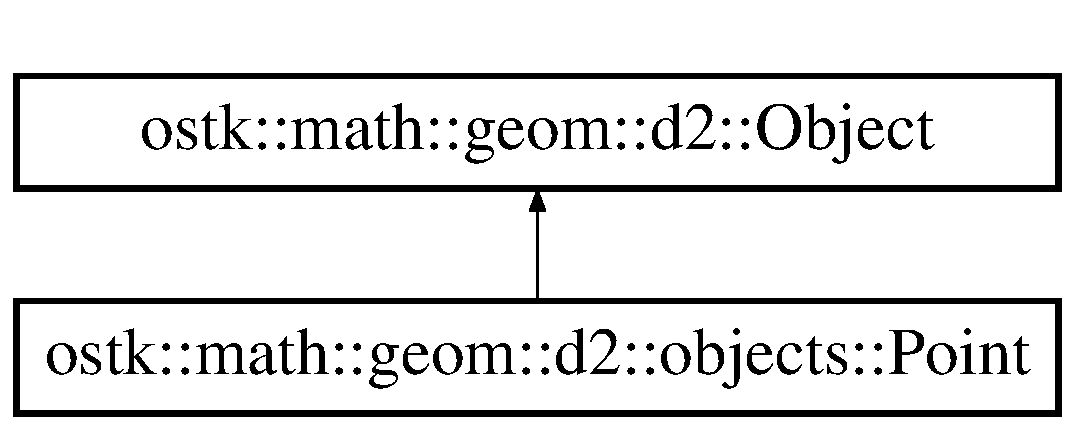
\includegraphics[height=2.000000cm]{classostk_1_1math_1_1geom_1_1d2_1_1objects_1_1_point}
\end{center}
\end{figure}
\doxysubsection*{Public Member Functions}
\begin{DoxyCompactItemize}
\item 
\mbox{\hyperlink{classostk_1_1math_1_1geom_1_1d2_1_1objects_1_1_point_ad4252af4171fbe3cff37ada7827e1966}{Point}} (const Real \&a\+First\+Coordinate, const Real \&a\+Second\+Coordinate)
\begin{DoxyCompactList}\small\item\em Constructor. \end{DoxyCompactList}\item 
virtual \mbox{\hyperlink{classostk_1_1math_1_1geom_1_1d2_1_1objects_1_1_point}{Point}} $\ast$ \mbox{\hyperlink{classostk_1_1math_1_1geom_1_1d2_1_1objects_1_1_point_a8550e9fe2c23c1f38e53093f4480598d}{clone}} () const override
\begin{DoxyCompactList}\small\item\em Clone point. \end{DoxyCompactList}\item 
bool \mbox{\hyperlink{classostk_1_1math_1_1geom_1_1d2_1_1objects_1_1_point_ad4dc9ca78b90f6c4a7e5da64a57b5d1f}{operator==}} (const \mbox{\hyperlink{classostk_1_1math_1_1geom_1_1d2_1_1objects_1_1_point}{Point}} \&a\+Point) const
\begin{DoxyCompactList}\small\item\em Equal to operator. \end{DoxyCompactList}\item 
bool \mbox{\hyperlink{classostk_1_1math_1_1geom_1_1d2_1_1objects_1_1_point_a2dd21e17403fe735ed517ef7f4212de2}{operator!=}} (const \mbox{\hyperlink{classostk_1_1math_1_1geom_1_1d2_1_1objects_1_1_point}{Point}} \&a\+Point) const
\begin{DoxyCompactList}\small\item\em Not equal to operator. \end{DoxyCompactList}\item 
virtual bool \mbox{\hyperlink{classostk_1_1math_1_1geom_1_1d2_1_1objects_1_1_point_a245dd2f0268e1f162804489ac911cb0c}{is\+Defined}} () const override
\begin{DoxyCompactList}\small\item\em Addition operator\+: translate point along vector. \end{DoxyCompactList}\item 
bool \mbox{\hyperlink{classostk_1_1math_1_1geom_1_1d2_1_1objects_1_1_point_aa9be8a5dd8b6d33398e0aba89308c71f}{is\+Near}} (const \mbox{\hyperlink{classostk_1_1math_1_1geom_1_1d2_1_1objects_1_1_point}{Point}} \&a\+Point, const Real \&a\+Tolerance) const
\begin{DoxyCompactList}\small\item\em Check if point is near another point. \end{DoxyCompactList}\item 
const Real \& \mbox{\hyperlink{classostk_1_1math_1_1geom_1_1d2_1_1objects_1_1_point_a59a7671f0609ce006479ae0d0f463e05}{x}} () const
\begin{DoxyCompactList}\small\item\em Get reference to first coordinate. \end{DoxyCompactList}\item 
const Real \& \mbox{\hyperlink{classostk_1_1math_1_1geom_1_1d2_1_1objects_1_1_point_a88caead5c128a3ca938506a8738ee279}{y}} () const
\begin{DoxyCompactList}\small\item\em Get reference to second coordinate. \end{DoxyCompactList}\item 
Vector2d \mbox{\hyperlink{classostk_1_1math_1_1geom_1_1d2_1_1objects_1_1_point_a19aa06ed436313a39c332caffcf2c86a}{as\+Vector}} () const
\begin{DoxyCompactList}\small\item\em Get vector representation of point. \end{DoxyCompactList}\item 
Real \mbox{\hyperlink{classostk_1_1math_1_1geom_1_1d2_1_1objects_1_1_point_a6e073732f59ff702531afbcaad286ec2}{distance\+To}} (const \mbox{\hyperlink{classostk_1_1math_1_1geom_1_1d2_1_1objects_1_1_point}{Point}} \&a\+Point) const
\begin{DoxyCompactList}\small\item\em Get distance to another point. \end{DoxyCompactList}\item 
virtual String \mbox{\hyperlink{classostk_1_1math_1_1geom_1_1d2_1_1objects_1_1_point_ac8fdaee79af60e2972257e43ff175f12}{to\+String}} (const \mbox{\hyperlink{classostk_1_1math_1_1geom_1_1d2_1_1_object_aa76f9e30caebf4005bafbdff447f66cf}{Object\+::\+Format}} \&a\+Format=\mbox{\hyperlink{classostk_1_1math_1_1geom_1_1d2_1_1_object_aa76f9e30caebf4005bafbdff447f66cfaeb6d8ae6f20283755b339c0dc273988b}{Object\+::\+Format\+::\+Standard}}, const Integer \&a\+Precision=Integer\+::\+Undefined()) const override
\begin{DoxyCompactList}\small\item\em Get string representation. \end{DoxyCompactList}\item 
virtual void \mbox{\hyperlink{classostk_1_1math_1_1geom_1_1d2_1_1objects_1_1_point_abcc3a265107dcccfcfe9349a6be788e5}{print}} (std\+::ostream \&an\+Output\+Stream, bool display\+Decorators=true) const override
\begin{DoxyCompactList}\small\item\em Print point. \end{DoxyCompactList}\item 
virtual void \mbox{\hyperlink{classostk_1_1math_1_1geom_1_1d2_1_1objects_1_1_point_aa880df23e5ee93a60dad85597c600fb0}{apply\+Transformation}} (const \mbox{\hyperlink{classostk_1_1math_1_1geom_1_1d2_1_1_transformation}{Transformation}} \&a\+Transformation) override
\begin{DoxyCompactList}\small\item\em Apply transformation to point. \end{DoxyCompactList}\end{DoxyCompactItemize}
\doxysubsection*{Static Public Member Functions}
\begin{DoxyCompactItemize}
\item 
static \mbox{\hyperlink{classostk_1_1math_1_1geom_1_1d2_1_1objects_1_1_point}{Point}} \mbox{\hyperlink{classostk_1_1math_1_1geom_1_1d2_1_1objects_1_1_point_a39c9ee703cfecf278ec2e9f3ffe4dac5}{Undefined}} ()
\begin{DoxyCompactList}\small\item\em Constructs an undefined point. \end{DoxyCompactList}\item 
static \mbox{\hyperlink{classostk_1_1math_1_1geom_1_1d2_1_1objects_1_1_point}{Point}} \mbox{\hyperlink{classostk_1_1math_1_1geom_1_1d2_1_1objects_1_1_point_a7b9fe974c947b8b1e1e2349c2a15a669}{Origin}} ()
\begin{DoxyCompactList}\small\item\em Constructs a point at origin. \end{DoxyCompactList}\item 
static \mbox{\hyperlink{classostk_1_1math_1_1geom_1_1d2_1_1objects_1_1_point}{Point}} \mbox{\hyperlink{classostk_1_1math_1_1geom_1_1d2_1_1objects_1_1_point_a6153f8ba851a8be99595d225632959af}{Vector}} (const Vector2d \&a\+Vector)
\begin{DoxyCompactList}\small\item\em Constructs a point from a vector. \end{DoxyCompactList}\end{DoxyCompactItemize}
\doxysubsection*{Additional Inherited Members}


\doxysubsection{Detailed Description}
\mbox{\hyperlink{classostk_1_1math_1_1geom_1_1d2_1_1objects_1_1_point}{Point}}. 

\href{https://en.wikipedia.org/wiki/Point_}{\texttt{ https\+://en.\+wikipedia.\+org/wiki/\+Point\+\_\+}}(geometry) 

\doxysubsection{Constructor \& Destructor Documentation}
\mbox{\Hypertarget{classostk_1_1math_1_1geom_1_1d2_1_1objects_1_1_point_ad4252af4171fbe3cff37ada7827e1966}\label{classostk_1_1math_1_1geom_1_1d2_1_1objects_1_1_point_ad4252af4171fbe3cff37ada7827e1966}} 
\index{ostk::math::geom::d2::objects::Point@{ostk::math::geom::d2::objects::Point}!Point@{Point}}
\index{Point@{Point}!ostk::math::geom::d2::objects::Point@{ostk::math::geom::d2::objects::Point}}
\doxysubsubsection{\texorpdfstring{Point()}{Point()}}
{\footnotesize\ttfamily ostk\+::math\+::geom\+::d2\+::objects\+::\+Point\+::\+Point (\begin{DoxyParamCaption}\item[{const Real \&}]{a\+First\+Coordinate,  }\item[{const Real \&}]{a\+Second\+Coordinate }\end{DoxyParamCaption})}



Constructor. 


\begin{DoxyCode}{0}
\DoxyCodeLine{\mbox{\hyperlink{classostk_1_1math_1_1geom_1_1d2_1_1objects_1_1_point_ad4252af4171fbe3cff37ada7827e1966}{Point}} point = \{ 0.0, 0.0 \} ;}
\end{DoxyCode}



\begin{DoxyParams}[1]{Parameters}
\mbox{\texttt{ in}}  & {\em a\+First\+Coordinate} & A first coordinate \\
\hline
\mbox{\texttt{ in}}  & {\em a\+Second\+Coordinate} & A second coordinate \\
\hline
\end{DoxyParams}


\doxysubsection{Member Function Documentation}
\mbox{\Hypertarget{classostk_1_1math_1_1geom_1_1d2_1_1objects_1_1_point_aa880df23e5ee93a60dad85597c600fb0}\label{classostk_1_1math_1_1geom_1_1d2_1_1objects_1_1_point_aa880df23e5ee93a60dad85597c600fb0}} 
\index{ostk::math::geom::d2::objects::Point@{ostk::math::geom::d2::objects::Point}!applyTransformation@{applyTransformation}}
\index{applyTransformation@{applyTransformation}!ostk::math::geom::d2::objects::Point@{ostk::math::geom::d2::objects::Point}}
\doxysubsubsection{\texorpdfstring{applyTransformation()}{applyTransformation()}}
{\footnotesize\ttfamily void ostk\+::math\+::geom\+::d2\+::objects\+::\+Point\+::apply\+Transformation (\begin{DoxyParamCaption}\item[{const \mbox{\hyperlink{classostk_1_1math_1_1geom_1_1d2_1_1_transformation}{Transformation}} \&}]{a\+Transformation }\end{DoxyParamCaption})\hspace{0.3cm}{\ttfamily [override]}, {\ttfamily [virtual]}}



Apply transformation to point. 


\begin{DoxyParams}[1]{Parameters}
\mbox{\texttt{ in}}  & {\em a\+Transformation} & A transformation \\
\hline
\end{DoxyParams}


Implements \mbox{\hyperlink{classostk_1_1math_1_1geom_1_1d2_1_1_object_a959e50211d7a680f7f904bbb752d75c9}{ostk\+::math\+::geom\+::d2\+::\+Object}}.

\mbox{\Hypertarget{classostk_1_1math_1_1geom_1_1d2_1_1objects_1_1_point_a19aa06ed436313a39c332caffcf2c86a}\label{classostk_1_1math_1_1geom_1_1d2_1_1objects_1_1_point_a19aa06ed436313a39c332caffcf2c86a}} 
\index{ostk::math::geom::d2::objects::Point@{ostk::math::geom::d2::objects::Point}!asVector@{asVector}}
\index{asVector@{asVector}!ostk::math::geom::d2::objects::Point@{ostk::math::geom::d2::objects::Point}}
\doxysubsubsection{\texorpdfstring{asVector()}{asVector()}}
{\footnotesize\ttfamily Vector2d ostk\+::math\+::geom\+::d2\+::objects\+::\+Point\+::as\+Vector (\begin{DoxyParamCaption}{ }\end{DoxyParamCaption}) const}



Get vector representation of point. 

\begin{DoxyReturn}{Returns}
Vector representation of point 
\end{DoxyReturn}
\mbox{\Hypertarget{classostk_1_1math_1_1geom_1_1d2_1_1objects_1_1_point_a8550e9fe2c23c1f38e53093f4480598d}\label{classostk_1_1math_1_1geom_1_1d2_1_1objects_1_1_point_a8550e9fe2c23c1f38e53093f4480598d}} 
\index{ostk::math::geom::d2::objects::Point@{ostk::math::geom::d2::objects::Point}!clone@{clone}}
\index{clone@{clone}!ostk::math::geom::d2::objects::Point@{ostk::math::geom::d2::objects::Point}}
\doxysubsubsection{\texorpdfstring{clone()}{clone()}}
{\footnotesize\ttfamily \mbox{\hyperlink{classostk_1_1math_1_1geom_1_1d2_1_1objects_1_1_point}{Point}} $\ast$ ostk\+::math\+::geom\+::d2\+::objects\+::\+Point\+::clone (\begin{DoxyParamCaption}{ }\end{DoxyParamCaption}) const\hspace{0.3cm}{\ttfamily [override]}, {\ttfamily [virtual]}}



Clone point. 

\begin{DoxyReturn}{Returns}
Pointer to cloned point 
\end{DoxyReturn}


Implements \mbox{\hyperlink{classostk_1_1math_1_1geom_1_1d2_1_1_object_a98dedc6792aef35308966ca768eb3e14}{ostk\+::math\+::geom\+::d2\+::\+Object}}.

\mbox{\Hypertarget{classostk_1_1math_1_1geom_1_1d2_1_1objects_1_1_point_a6e073732f59ff702531afbcaad286ec2}\label{classostk_1_1math_1_1geom_1_1d2_1_1objects_1_1_point_a6e073732f59ff702531afbcaad286ec2}} 
\index{ostk::math::geom::d2::objects::Point@{ostk::math::geom::d2::objects::Point}!distanceTo@{distanceTo}}
\index{distanceTo@{distanceTo}!ostk::math::geom::d2::objects::Point@{ostk::math::geom::d2::objects::Point}}
\doxysubsubsection{\texorpdfstring{distanceTo()}{distanceTo()}}
{\footnotesize\ttfamily Real ostk\+::math\+::geom\+::d2\+::objects\+::\+Point\+::distance\+To (\begin{DoxyParamCaption}\item[{const \mbox{\hyperlink{classostk_1_1math_1_1geom_1_1d2_1_1objects_1_1_point}{Point}} \&}]{a\+Point }\end{DoxyParamCaption}) const}



Get distance to another point. 


\begin{DoxyParams}[1]{Parameters}
\mbox{\texttt{ in}}  & {\em a\+Point} & A point \\
\hline
\end{DoxyParams}
\begin{DoxyReturn}{Returns}
Distance to point 
\end{DoxyReturn}
\mbox{\Hypertarget{classostk_1_1math_1_1geom_1_1d2_1_1objects_1_1_point_a245dd2f0268e1f162804489ac911cb0c}\label{classostk_1_1math_1_1geom_1_1d2_1_1objects_1_1_point_a245dd2f0268e1f162804489ac911cb0c}} 
\index{ostk::math::geom::d2::objects::Point@{ostk::math::geom::d2::objects::Point}!isDefined@{isDefined}}
\index{isDefined@{isDefined}!ostk::math::geom::d2::objects::Point@{ostk::math::geom::d2::objects::Point}}
\doxysubsubsection{\texorpdfstring{isDefined()}{isDefined()}}
{\footnotesize\ttfamily bool ostk\+::math\+::geom\+::d2\+::objects\+::\+Point\+::is\+Defined (\begin{DoxyParamCaption}{ }\end{DoxyParamCaption}) const\hspace{0.3cm}{\ttfamily [override]}, {\ttfamily [virtual]}}



Addition operator\+: translate point along vector. 


\begin{DoxyCode}{0}
\DoxyCodeLine{                        \mbox{\hyperlink{classostk_1_1math_1_1geom_1_1d2_1_1objects_1_1_point_ad4252af4171fbe3cff37ada7827e1966}{Point}}(0.0, 0.0) + \mbox{\hyperlink{namespaceostk_1_1math_1_1obj_a5ce374bc225ecfb685da4fed9aa67e6e}{Vector2d}}(0.0, 1.0) ; \textcolor{comment}{// [0.0, 1.0]}}
\DoxyCodeLine{    @encode}
\DoxyCodeLine{   }
\DoxyCodeLine{    @param              [in] aVector A translation vector}
\DoxyCodeLine{    @\textcolor{keywordflow}{return}             A point}
\DoxyCodeLine{}
\DoxyCodeLine{\mbox{\hyperlink{classostk_1_1math_1_1geom_1_1d2_1_1objects_1_1_point_ad4252af4171fbe3cff37ada7827e1966}{Point}}                   operator +                                  (   \textcolor{keyword}{const}   \mbox{\hyperlink{namespaceostk_1_1math_1_1obj_a5ce374bc225ecfb685da4fed9aa67e6e}{Vector2d}}\&                   aVector                                     ) \textcolor{keyword}{const} ;}
\DoxyCodeLine{}
\DoxyCodeLine{    @brief              Subtraction \textcolor{keyword}{operator}: translate point along opposite vector}
\DoxyCodeLine{   }
\DoxyCodeLine{    @code}
\DoxyCodeLine{                        \mbox{\hyperlink{classostk_1_1math_1_1geom_1_1d2_1_1objects_1_1_point_ad4252af4171fbe3cff37ada7827e1966}{Point}}(0.0, 1.0) -\/ \mbox{\hyperlink{namespaceostk_1_1math_1_1obj_a5ce374bc225ecfb685da4fed9aa67e6e}{Vector2d}}(0.0, 1.0) ; \textcolor{comment}{// [0.0, 0.0]}}
\DoxyCodeLine{    @encode}
\DoxyCodeLine{   }
\DoxyCodeLine{    @param              [in] aVector A translation vector}
\DoxyCodeLine{    @\textcolor{keywordflow}{return}             A point}
\DoxyCodeLine{}
\DoxyCodeLine{\mbox{\hyperlink{classostk_1_1math_1_1geom_1_1d2_1_1objects_1_1_point_ad4252af4171fbe3cff37ada7827e1966}{Point}}                   operator -\/                                  (   \textcolor{keyword}{const}   \mbox{\hyperlink{namespaceostk_1_1math_1_1obj_a5ce374bc225ecfb685da4fed9aa67e6e}{Vector2d}}\&                   aVector                                     ) \textcolor{keyword}{const} ;}
\DoxyCodeLine{}
\DoxyCodeLine{    @brief              Subtraction \textcolor{keyword}{operator}: get translation vector between two points}
\DoxyCodeLine{   }
\DoxyCodeLine{    @code}
\DoxyCodeLine{                        \mbox{\hyperlink{classostk_1_1math_1_1geom_1_1d2_1_1objects_1_1_point_ad4252af4171fbe3cff37ada7827e1966}{Point}}(0.0, 1.0) -\/ \mbox{\hyperlink{classostk_1_1math_1_1geom_1_1d2_1_1objects_1_1_point_ad4252af4171fbe3cff37ada7827e1966}{Point}}(0.0, 0.0)  ; \textcolor{comment}{// [0.0, 1.0]}}
\DoxyCodeLine{    @encode}
\DoxyCodeLine{   }
\DoxyCodeLine{    @param              [in] aPoint A point}
\DoxyCodeLine{    @\textcolor{keywordflow}{return}             A translation vector}
\DoxyCodeLine{}
\DoxyCodeLine{\mbox{\hyperlink{namespaceostk_1_1math_1_1obj_a5ce374bc225ecfb685da4fed9aa67e6e}{Vector2d}}                operator -\/                                  (   \textcolor{keyword}{const}   \mbox{\hyperlink{classostk_1_1math_1_1geom_1_1d2_1_1objects_1_1_point_ad4252af4171fbe3cff37ada7827e1966}{Point}}\&                      aPoint                                      ) \textcolor{keyword}{const} ;}
\DoxyCodeLine{}
\DoxyCodeLine{    @brief              Check \textcolor{keywordflow}{if} point is defined}
\DoxyCodeLine{   }
\DoxyCodeLine{    @code}
\DoxyCodeLine{                        \mbox{\hyperlink{classostk_1_1math_1_1geom_1_1d2_1_1objects_1_1_point_ad4252af4171fbe3cff37ada7827e1966}{Point}}(0.0, 0.0).isDefined() ; \textcolor{comment}{// True}}
\end{DoxyCode}


\begin{DoxyReturn}{Returns}
True if point is defined 
\end{DoxyReturn}


Implements \mbox{\hyperlink{classostk_1_1math_1_1geom_1_1d2_1_1_object_a456cc7121218d24c1322d0fe54230cc4}{ostk\+::math\+::geom\+::d2\+::\+Object}}.

\mbox{\Hypertarget{classostk_1_1math_1_1geom_1_1d2_1_1objects_1_1_point_aa9be8a5dd8b6d33398e0aba89308c71f}\label{classostk_1_1math_1_1geom_1_1d2_1_1objects_1_1_point_aa9be8a5dd8b6d33398e0aba89308c71f}} 
\index{ostk::math::geom::d2::objects::Point@{ostk::math::geom::d2::objects::Point}!isNear@{isNear}}
\index{isNear@{isNear}!ostk::math::geom::d2::objects::Point@{ostk::math::geom::d2::objects::Point}}
\doxysubsubsection{\texorpdfstring{isNear()}{isNear()}}
{\footnotesize\ttfamily bool ostk\+::math\+::geom\+::d2\+::objects\+::\+Point\+::is\+Near (\begin{DoxyParamCaption}\item[{const \mbox{\hyperlink{classostk_1_1math_1_1geom_1_1d2_1_1objects_1_1_point}{Point}} \&}]{a\+Point,  }\item[{const Real \&}]{a\+Tolerance }\end{DoxyParamCaption}) const}



Check if point is near another point. 


\begin{DoxyCode}{0}
\DoxyCodeLine{\mbox{\hyperlink{classostk_1_1math_1_1geom_1_1d2_1_1objects_1_1_point_ad4252af4171fbe3cff37ada7827e1966}{Point}}(0.0, 0.0).isNear(\mbox{\hyperlink{classostk_1_1math_1_1geom_1_1d2_1_1objects_1_1_point_ad4252af4171fbe3cff37ada7827e1966}{Point}}(0.0, 0.0), 1e-\/15) ; \textcolor{comment}{// True}}
\end{DoxyCode}



\begin{DoxyParams}[1]{Parameters}
\mbox{\texttt{ in}}  & {\em a\+Point} & A point \\
\hline
\mbox{\texttt{ in}}  & {\em a\+Tolerance} & A tolerance \\
\hline
\end{DoxyParams}
\begin{DoxyReturn}{Returns}
True if point is near another point 
\end{DoxyReturn}
\mbox{\Hypertarget{classostk_1_1math_1_1geom_1_1d2_1_1objects_1_1_point_a2dd21e17403fe735ed517ef7f4212de2}\label{classostk_1_1math_1_1geom_1_1d2_1_1objects_1_1_point_a2dd21e17403fe735ed517ef7f4212de2}} 
\index{ostk::math::geom::d2::objects::Point@{ostk::math::geom::d2::objects::Point}!operator"!=@{operator"!=}}
\index{operator"!=@{operator"!=}!ostk::math::geom::d2::objects::Point@{ostk::math::geom::d2::objects::Point}}
\doxysubsubsection{\texorpdfstring{operator"!=()}{operator!=()}}
{\footnotesize\ttfamily bool ostk\+::math\+::geom\+::d2\+::objects\+::\+Point\+::operator!= (\begin{DoxyParamCaption}\item[{const \mbox{\hyperlink{classostk_1_1math_1_1geom_1_1d2_1_1objects_1_1_point}{Point}} \&}]{a\+Point }\end{DoxyParamCaption}) const}



Not equal to operator. 


\begin{DoxyParams}[1]{Parameters}
\mbox{\texttt{ in}}  & {\em a\+Point} & A point \\
\hline
\end{DoxyParams}
\begin{DoxyReturn}{Returns}
True if points are not equal 
\end{DoxyReturn}
\mbox{\Hypertarget{classostk_1_1math_1_1geom_1_1d2_1_1objects_1_1_point_ad4dc9ca78b90f6c4a7e5da64a57b5d1f}\label{classostk_1_1math_1_1geom_1_1d2_1_1objects_1_1_point_ad4dc9ca78b90f6c4a7e5da64a57b5d1f}} 
\index{ostk::math::geom::d2::objects::Point@{ostk::math::geom::d2::objects::Point}!operator==@{operator==}}
\index{operator==@{operator==}!ostk::math::geom::d2::objects::Point@{ostk::math::geom::d2::objects::Point}}
\doxysubsubsection{\texorpdfstring{operator==()}{operator==()}}
{\footnotesize\ttfamily bool ostk\+::math\+::geom\+::d2\+::objects\+::\+Point\+::operator== (\begin{DoxyParamCaption}\item[{const \mbox{\hyperlink{classostk_1_1math_1_1geom_1_1d2_1_1objects_1_1_point}{Point}} \&}]{a\+Point }\end{DoxyParamCaption}) const}



Equal to operator. 


\begin{DoxyParams}[1]{Parameters}
\mbox{\texttt{ in}}  & {\em a\+Point} & A point \\
\hline
\end{DoxyParams}
\begin{DoxyReturn}{Returns}
True if points are equal 
\end{DoxyReturn}
\mbox{\Hypertarget{classostk_1_1math_1_1geom_1_1d2_1_1objects_1_1_point_a7b9fe974c947b8b1e1e2349c2a15a669}\label{classostk_1_1math_1_1geom_1_1d2_1_1objects_1_1_point_a7b9fe974c947b8b1e1e2349c2a15a669}} 
\index{ostk::math::geom::d2::objects::Point@{ostk::math::geom::d2::objects::Point}!Origin@{Origin}}
\index{Origin@{Origin}!ostk::math::geom::d2::objects::Point@{ostk::math::geom::d2::objects::Point}}
\doxysubsubsection{\texorpdfstring{Origin()}{Origin()}}
{\footnotesize\ttfamily \mbox{\hyperlink{classostk_1_1math_1_1geom_1_1d2_1_1objects_1_1_point}{Point}} ostk\+::math\+::geom\+::d2\+::objects\+::\+Point\+::\+Origin (\begin{DoxyParamCaption}{ }\end{DoxyParamCaption})\hspace{0.3cm}{\ttfamily [static]}}



Constructs a point at origin. 


\begin{DoxyCode}{0}
\DoxyCodeLine{\mbox{\hyperlink{classostk_1_1math_1_1geom_1_1d2_1_1objects_1_1_point_ad4252af4171fbe3cff37ada7827e1966}{Point}} point = \mbox{\hyperlink{classostk_1_1math_1_1geom_1_1d2_1_1objects_1_1_point_a7b9fe974c947b8b1e1e2349c2a15a669}{Point::Origin}}() ; \textcolor{comment}{// [0.0, 0.0]}}
\end{DoxyCode}


\begin{DoxyReturn}{Returns}
\mbox{\hyperlink{classostk_1_1math_1_1geom_1_1d2_1_1objects_1_1_point}{Point}} at origin 
\end{DoxyReturn}
\mbox{\Hypertarget{classostk_1_1math_1_1geom_1_1d2_1_1objects_1_1_point_abcc3a265107dcccfcfe9349a6be788e5}\label{classostk_1_1math_1_1geom_1_1d2_1_1objects_1_1_point_abcc3a265107dcccfcfe9349a6be788e5}} 
\index{ostk::math::geom::d2::objects::Point@{ostk::math::geom::d2::objects::Point}!print@{print}}
\index{print@{print}!ostk::math::geom::d2::objects::Point@{ostk::math::geom::d2::objects::Point}}
\doxysubsubsection{\texorpdfstring{print()}{print()}}
{\footnotesize\ttfamily void ostk\+::math\+::geom\+::d2\+::objects\+::\+Point\+::print (\begin{DoxyParamCaption}\item[{std\+::ostream \&}]{an\+Output\+Stream,  }\item[{bool}]{display\+Decorators = {\ttfamily true} }\end{DoxyParamCaption}) const\hspace{0.3cm}{\ttfamily [override]}, {\ttfamily [virtual]}}



Print point. 


\begin{DoxyParams}[1]{Parameters}
\mbox{\texttt{ in}}  & {\em an\+Output\+Stream} & An output stream \\
\hline
\mbox{\texttt{ in}}  & {\em (optional)} & display\+Decorators If true, display decorators \\
\hline
\end{DoxyParams}


Implements \mbox{\hyperlink{classostk_1_1math_1_1geom_1_1d2_1_1_object_ae05ad883ed5a560e38f0aae7a4adc1ea}{ostk\+::math\+::geom\+::d2\+::\+Object}}.

\mbox{\Hypertarget{classostk_1_1math_1_1geom_1_1d2_1_1objects_1_1_point_ac8fdaee79af60e2972257e43ff175f12}\label{classostk_1_1math_1_1geom_1_1d2_1_1objects_1_1_point_ac8fdaee79af60e2972257e43ff175f12}} 
\index{ostk::math::geom::d2::objects::Point@{ostk::math::geom::d2::objects::Point}!toString@{toString}}
\index{toString@{toString}!ostk::math::geom::d2::objects::Point@{ostk::math::geom::d2::objects::Point}}
\doxysubsubsection{\texorpdfstring{toString()}{toString()}}
{\footnotesize\ttfamily String ostk\+::math\+::geom\+::d2\+::objects\+::\+Point\+::to\+String (\begin{DoxyParamCaption}\item[{const \mbox{\hyperlink{classostk_1_1math_1_1geom_1_1d2_1_1_object_aa76f9e30caebf4005bafbdff447f66cf}{Object\+::\+Format}} \&}]{a\+Format = {\ttfamily \mbox{\hyperlink{classostk_1_1math_1_1geom_1_1d2_1_1_object_aa76f9e30caebf4005bafbdff447f66cfaeb6d8ae6f20283755b339c0dc273988b}{Object\+::\+Format\+::\+Standard}}},  }\item[{const Integer \&}]{a\+Precision = {\ttfamily Integer\+:\+:Undefined()} }\end{DoxyParamCaption}) const\hspace{0.3cm}{\ttfamily [override]}, {\ttfamily [virtual]}}



Get string representation. 


\begin{DoxyParams}[1]{Parameters}
\mbox{\texttt{ in}}  & {\em a\+Format} & A format \\
\hline
\mbox{\texttt{ in}}  & {\em (optional)} & a\+Precision A precision \\
\hline
\end{DoxyParams}
\begin{DoxyReturn}{Returns}
String representation 
\end{DoxyReturn}


Implements \mbox{\hyperlink{classostk_1_1math_1_1geom_1_1d2_1_1_object_ada4c2187dd24ef02b91b6346191f677c}{ostk\+::math\+::geom\+::d2\+::\+Object}}.

\mbox{\Hypertarget{classostk_1_1math_1_1geom_1_1d2_1_1objects_1_1_point_a39c9ee703cfecf278ec2e9f3ffe4dac5}\label{classostk_1_1math_1_1geom_1_1d2_1_1objects_1_1_point_a39c9ee703cfecf278ec2e9f3ffe4dac5}} 
\index{ostk::math::geom::d2::objects::Point@{ostk::math::geom::d2::objects::Point}!Undefined@{Undefined}}
\index{Undefined@{Undefined}!ostk::math::geom::d2::objects::Point@{ostk::math::geom::d2::objects::Point}}
\doxysubsubsection{\texorpdfstring{Undefined()}{Undefined()}}
{\footnotesize\ttfamily \mbox{\hyperlink{classostk_1_1math_1_1geom_1_1d2_1_1objects_1_1_point}{Point}} ostk\+::math\+::geom\+::d2\+::objects\+::\+Point\+::\+Undefined (\begin{DoxyParamCaption}{ }\end{DoxyParamCaption})\hspace{0.3cm}{\ttfamily [static]}}



Constructs an undefined point. 


\begin{DoxyCode}{0}
\DoxyCodeLine{\mbox{\hyperlink{classostk_1_1math_1_1geom_1_1d2_1_1objects_1_1_point_ad4252af4171fbe3cff37ada7827e1966}{Point}} point = \mbox{\hyperlink{classostk_1_1math_1_1geom_1_1d2_1_1objects_1_1_point_a39c9ee703cfecf278ec2e9f3ffe4dac5}{Point::Undefined}}() ; \textcolor{comment}{// Undefined}}
\end{DoxyCode}


\begin{DoxyReturn}{Returns}
Undefined point 
\end{DoxyReturn}
\mbox{\Hypertarget{classostk_1_1math_1_1geom_1_1d2_1_1objects_1_1_point_a6153f8ba851a8be99595d225632959af}\label{classostk_1_1math_1_1geom_1_1d2_1_1objects_1_1_point_a6153f8ba851a8be99595d225632959af}} 
\index{ostk::math::geom::d2::objects::Point@{ostk::math::geom::d2::objects::Point}!Vector@{Vector}}
\index{Vector@{Vector}!ostk::math::geom::d2::objects::Point@{ostk::math::geom::d2::objects::Point}}
\doxysubsubsection{\texorpdfstring{Vector()}{Vector()}}
{\footnotesize\ttfamily \mbox{\hyperlink{classostk_1_1math_1_1geom_1_1d2_1_1objects_1_1_point}{Point}} ostk\+::math\+::geom\+::d2\+::objects\+::\+Point\+::\+Vector (\begin{DoxyParamCaption}\item[{const Vector2d \&}]{a\+Vector }\end{DoxyParamCaption})\hspace{0.3cm}{\ttfamily [static]}}



Constructs a point from a vector. 


\begin{DoxyCode}{0}
\DoxyCodeLine{\mbox{\hyperlink{classostk_1_1math_1_1geom_1_1d2_1_1objects_1_1_point_ad4252af4171fbe3cff37ada7827e1966}{Point}} point = \mbox{\hyperlink{classostk_1_1math_1_1geom_1_1d2_1_1objects_1_1_point_a6153f8ba851a8be99595d225632959af}{Point::Vector}}(\{ 0.0, 0.0 \}) ; \textcolor{comment}{// [0.0, 0.0]}}
\end{DoxyCode}


\begin{DoxyReturn}{Returns}
\mbox{\hyperlink{classostk_1_1math_1_1geom_1_1d2_1_1objects_1_1_point}{Point}} 
\end{DoxyReturn}
\mbox{\Hypertarget{classostk_1_1math_1_1geom_1_1d2_1_1objects_1_1_point_a59a7671f0609ce006479ae0d0f463e05}\label{classostk_1_1math_1_1geom_1_1d2_1_1objects_1_1_point_a59a7671f0609ce006479ae0d0f463e05}} 
\index{ostk::math::geom::d2::objects::Point@{ostk::math::geom::d2::objects::Point}!x@{x}}
\index{x@{x}!ostk::math::geom::d2::objects::Point@{ostk::math::geom::d2::objects::Point}}
\doxysubsubsection{\texorpdfstring{x()}{x()}}
{\footnotesize\ttfamily const Real \& ostk\+::math\+::geom\+::d2\+::objects\+::\+Point\+::x (\begin{DoxyParamCaption}{ }\end{DoxyParamCaption}) const}



Get reference to first coordinate. 


\begin{DoxyCode}{0}
\DoxyCodeLine{\mbox{\hyperlink{classostk_1_1math_1_1geom_1_1d2_1_1objects_1_1_point_ad4252af4171fbe3cff37ada7827e1966}{Point}}(1.0, 2.0).x() ; \textcolor{comment}{// \&1.0}}
\end{DoxyCode}


\begin{DoxyReturn}{Returns}
Reference to first coordinate 
\end{DoxyReturn}
\mbox{\Hypertarget{classostk_1_1math_1_1geom_1_1d2_1_1objects_1_1_point_a88caead5c128a3ca938506a8738ee279}\label{classostk_1_1math_1_1geom_1_1d2_1_1objects_1_1_point_a88caead5c128a3ca938506a8738ee279}} 
\index{ostk::math::geom::d2::objects::Point@{ostk::math::geom::d2::objects::Point}!y@{y}}
\index{y@{y}!ostk::math::geom::d2::objects::Point@{ostk::math::geom::d2::objects::Point}}
\doxysubsubsection{\texorpdfstring{y()}{y()}}
{\footnotesize\ttfamily const Real \& ostk\+::math\+::geom\+::d2\+::objects\+::\+Point\+::y (\begin{DoxyParamCaption}{ }\end{DoxyParamCaption}) const}



Get reference to second coordinate. 


\begin{DoxyCode}{0}
\DoxyCodeLine{\mbox{\hyperlink{classostk_1_1math_1_1geom_1_1d2_1_1objects_1_1_point_ad4252af4171fbe3cff37ada7827e1966}{Point}}(1.0, 2.0).y() ; \textcolor{comment}{// \&2.0}}
\end{DoxyCode}


\begin{DoxyReturn}{Returns}
Reference to second coordinate 
\end{DoxyReturn}


The documentation for this class was generated from the following files\+:\begin{DoxyCompactItemize}
\item 
include/\+Open\+Space\+Toolkit/\+Mathematics/\+Geometry/2\+D/\+Objects/\mbox{\hyperlink{2_d_2_objects_2_point_8hpp}{Point.\+hpp}}\item 
src/\+Open\+Space\+Toolkit/\+Mathematics/\+Geometry/2\+D/\+Objects/\mbox{\hyperlink{2_d_2_objects_2_point_8cpp}{Point.\+cpp}}\end{DoxyCompactItemize}

\hypertarget{classostk_1_1math_1_1geom_1_1d3_1_1objects_1_1_point}{}\doxysection{ostk\+::math\+::geom\+::d3\+::objects\+::Point Class Reference}
\label{classostk_1_1math_1_1geom_1_1d3_1_1objects_1_1_point}\index{ostk::math::geom::d3::objects::Point@{ostk::math::geom::d3::objects::Point}}


\mbox{\hyperlink{classostk_1_1math_1_1geom_1_1d3_1_1objects_1_1_point}{Point}}.  




{\ttfamily \#include $<$Point.\+hpp$>$}

Inheritance diagram for ostk\+::math\+::geom\+::d3\+::objects\+::Point\+:\begin{figure}[H]
\begin{center}
\leavevmode
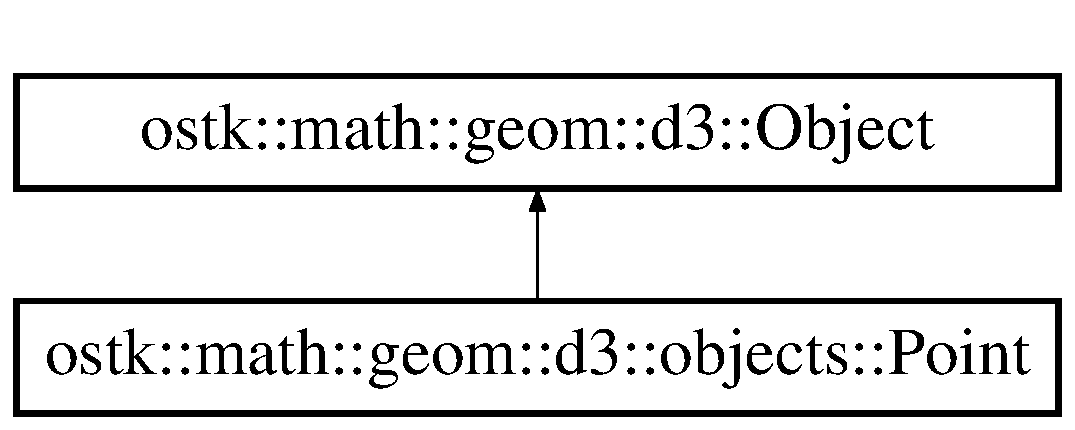
\includegraphics[height=2.000000cm]{classostk_1_1math_1_1geom_1_1d3_1_1objects_1_1_point}
\end{center}
\end{figure}
\doxysubsection*{Public Member Functions}
\begin{DoxyCompactItemize}
\item 
\mbox{\hyperlink{classostk_1_1math_1_1geom_1_1d3_1_1objects_1_1_point_ad9bee5dadb878200f859b20a34680ae5}{Point}} (const Real \&a\+First\+Coordinate, const Real \&a\+Second\+Coordinate, const Real \&a\+Third\+Coordinate)
\begin{DoxyCompactList}\small\item\em Constructor. \end{DoxyCompactList}\item 
virtual \mbox{\hyperlink{classostk_1_1math_1_1geom_1_1d3_1_1objects_1_1_point}{Point}} $\ast$ \mbox{\hyperlink{classostk_1_1math_1_1geom_1_1d3_1_1objects_1_1_point_aeee85a494568471d821310dc14b5b9d5}{clone}} () const override
\begin{DoxyCompactList}\small\item\em Clone point. \end{DoxyCompactList}\item 
bool \mbox{\hyperlink{classostk_1_1math_1_1geom_1_1d3_1_1objects_1_1_point_a572b7054bc9c2e9b7de13449f5a801e1}{operator==}} (const \mbox{\hyperlink{classostk_1_1math_1_1geom_1_1d3_1_1objects_1_1_point}{Point}} \&a\+Point) const
\begin{DoxyCompactList}\small\item\em Equal to operator. \end{DoxyCompactList}\item 
bool \mbox{\hyperlink{classostk_1_1math_1_1geom_1_1d3_1_1objects_1_1_point_a8203b4594dca180e254463abf0043526}{operator!=}} (const \mbox{\hyperlink{classostk_1_1math_1_1geom_1_1d3_1_1objects_1_1_point}{Point}} \&a\+Point) const
\begin{DoxyCompactList}\small\item\em Not equal to operator. \end{DoxyCompactList}\item 
virtual bool \mbox{\hyperlink{classostk_1_1math_1_1geom_1_1d3_1_1objects_1_1_point_ad7e8b8a4f1bae1c6cd0d5895996d65b7}{is\+Defined}} () const override
\begin{DoxyCompactList}\small\item\em Addition operator\+: translate point along vector. \end{DoxyCompactList}\item 
bool \mbox{\hyperlink{classostk_1_1math_1_1geom_1_1d3_1_1objects_1_1_point_abeeb9784820f7835e352cdbcd62c073a}{is\+Near}} (const \mbox{\hyperlink{classostk_1_1math_1_1geom_1_1d3_1_1objects_1_1_point}{Point}} \&a\+Point, const Real \&a\+Tolerance) const
\begin{DoxyCompactList}\small\item\em Check if point is near another point. \end{DoxyCompactList}\item 
const Real \& \mbox{\hyperlink{classostk_1_1math_1_1geom_1_1d3_1_1objects_1_1_point_a68a5204a2ca259486a1c1e442c833203}{x}} () const
\begin{DoxyCompactList}\small\item\em Get reference to first coordinate. \end{DoxyCompactList}\item 
const Real \& \mbox{\hyperlink{classostk_1_1math_1_1geom_1_1d3_1_1objects_1_1_point_a77c908e2091fa581f8e975824dbe4f22}{y}} () const
\begin{DoxyCompactList}\small\item\em Get reference to second coordinate. \end{DoxyCompactList}\item 
const Real \& \mbox{\hyperlink{classostk_1_1math_1_1geom_1_1d3_1_1objects_1_1_point_a16b88664b655d69c146421dfb75bc246}{z}} () const
\begin{DoxyCompactList}\small\item\em Get reference to third coordinate. \end{DoxyCompactList}\item 
Vector3d \mbox{\hyperlink{classostk_1_1math_1_1geom_1_1d3_1_1objects_1_1_point_a00034296a5aab3bcc8c4fe46584f119a}{as\+Vector}} () const
\begin{DoxyCompactList}\small\item\em Get vector representation of point. \end{DoxyCompactList}\item 
Real \mbox{\hyperlink{classostk_1_1math_1_1geom_1_1d3_1_1objects_1_1_point_a17c835ac01d24fb703eee44191331ee7}{distance\+To}} (const \mbox{\hyperlink{classostk_1_1math_1_1geom_1_1d3_1_1objects_1_1_point}{Point}} \&a\+Point) const
\begin{DoxyCompactList}\small\item\em Get distance to another point. \end{DoxyCompactList}\item 
String \mbox{\hyperlink{classostk_1_1math_1_1geom_1_1d3_1_1objects_1_1_point_a86208d5df1931b6d847e74dd99406e70}{to\+String}} (const Integer \&a\+Precision=\mbox{\hyperlink{3_d_2_objects_2_point_8hpp_a6d81881a7883657dbc659ca545d9085d}{D\+E\+F\+A\+U\+L\+T\+\_\+\+P\+R\+E\+C\+I\+S\+I\+ON}}) const
\begin{DoxyCompactList}\small\item\em Get string representation. \end{DoxyCompactList}\item 
virtual void \mbox{\hyperlink{classostk_1_1math_1_1geom_1_1d3_1_1objects_1_1_point_a9aa69f544cb1b2b521126c0cca39c951}{print}} (std\+::ostream \&an\+Output\+Stream, bool display\+Decorators=true) const override
\begin{DoxyCompactList}\small\item\em Print point. \end{DoxyCompactList}\item 
virtual void \mbox{\hyperlink{classostk_1_1math_1_1geom_1_1d3_1_1objects_1_1_point_a0b79a5726ac04f814b8a5b737daf0028}{apply\+Transformation}} (const \mbox{\hyperlink{classostk_1_1math_1_1geom_1_1d3_1_1_transformation}{Transformation}} \&a\+Transformation) override
\begin{DoxyCompactList}\small\item\em Apply transformation to point. \end{DoxyCompactList}\end{DoxyCompactItemize}
\doxysubsection*{Static Public Member Functions}
\begin{DoxyCompactItemize}
\item 
static \mbox{\hyperlink{classostk_1_1math_1_1geom_1_1d3_1_1objects_1_1_point}{Point}} \mbox{\hyperlink{classostk_1_1math_1_1geom_1_1d3_1_1objects_1_1_point_ab0de3c7a7d547bbf169d0beb62f9ea25}{Undefined}} ()
\begin{DoxyCompactList}\small\item\em Constructs an undefined point. \end{DoxyCompactList}\item 
static \mbox{\hyperlink{classostk_1_1math_1_1geom_1_1d3_1_1objects_1_1_point}{Point}} \mbox{\hyperlink{classostk_1_1math_1_1geom_1_1d3_1_1objects_1_1_point_a079c199f08b015d456d02728a71b534c}{Origin}} ()
\begin{DoxyCompactList}\small\item\em Constructs a point at origin. \end{DoxyCompactList}\item 
static \mbox{\hyperlink{classostk_1_1math_1_1geom_1_1d3_1_1objects_1_1_point}{Point}} \mbox{\hyperlink{classostk_1_1math_1_1geom_1_1d3_1_1objects_1_1_point_a74796fec8c39081bc8d766d70e44651d}{Vector}} (const Vector3d \&a\+Vector)
\begin{DoxyCompactList}\small\item\em Constructs a point from a vector. \end{DoxyCompactList}\end{DoxyCompactItemize}


\doxysubsection{Detailed Description}
\mbox{\hyperlink{classostk_1_1math_1_1geom_1_1d3_1_1objects_1_1_point}{Point}}. 

\href{https://en.wikipedia.org/wiki/Point_}{\texttt{ https\+://en.\+wikipedia.\+org/wiki/\+Point\+\_\+}}(geometry) 

\doxysubsection{Constructor \& Destructor Documentation}
\mbox{\Hypertarget{classostk_1_1math_1_1geom_1_1d3_1_1objects_1_1_point_ad9bee5dadb878200f859b20a34680ae5}\label{classostk_1_1math_1_1geom_1_1d3_1_1objects_1_1_point_ad9bee5dadb878200f859b20a34680ae5}} 
\index{ostk::math::geom::d3::objects::Point@{ostk::math::geom::d3::objects::Point}!Point@{Point}}
\index{Point@{Point}!ostk::math::geom::d3::objects::Point@{ostk::math::geom::d3::objects::Point}}
\doxysubsubsection{\texorpdfstring{Point()}{Point()}}
{\footnotesize\ttfamily ostk\+::math\+::geom\+::d3\+::objects\+::\+Point\+::\+Point (\begin{DoxyParamCaption}\item[{const Real \&}]{a\+First\+Coordinate,  }\item[{const Real \&}]{a\+Second\+Coordinate,  }\item[{const Real \&}]{a\+Third\+Coordinate }\end{DoxyParamCaption})}



Constructor. 


\begin{DoxyCode}{0}
\DoxyCodeLine{\mbox{\hyperlink{classostk_1_1math_1_1geom_1_1d3_1_1objects_1_1_point_ad9bee5dadb878200f859b20a34680ae5}{Point}} point(0.0, 0.0, 0.0) ;}
\end{DoxyCode}



\begin{DoxyParams}[1]{Parameters}
\mbox{\texttt{ in}}  & {\em a\+First\+Coordinate} & A first coordinate \\
\hline
\mbox{\texttt{ in}}  & {\em a\+Second\+Coordinate} & A second coordinate \\
\hline
\mbox{\texttt{ in}}  & {\em a\+Third\+Coordinate} & A third coordinate \\
\hline
\end{DoxyParams}


\doxysubsection{Member Function Documentation}
\mbox{\Hypertarget{classostk_1_1math_1_1geom_1_1d3_1_1objects_1_1_point_a0b79a5726ac04f814b8a5b737daf0028}\label{classostk_1_1math_1_1geom_1_1d3_1_1objects_1_1_point_a0b79a5726ac04f814b8a5b737daf0028}} 
\index{ostk::math::geom::d3::objects::Point@{ostk::math::geom::d3::objects::Point}!applyTransformation@{applyTransformation}}
\index{applyTransformation@{applyTransformation}!ostk::math::geom::d3::objects::Point@{ostk::math::geom::d3::objects::Point}}
\doxysubsubsection{\texorpdfstring{applyTransformation()}{applyTransformation()}}
{\footnotesize\ttfamily void ostk\+::math\+::geom\+::d3\+::objects\+::\+Point\+::apply\+Transformation (\begin{DoxyParamCaption}\item[{const \mbox{\hyperlink{classostk_1_1math_1_1geom_1_1d3_1_1_transformation}{Transformation}} \&}]{a\+Transformation }\end{DoxyParamCaption})\hspace{0.3cm}{\ttfamily [override]}, {\ttfamily [virtual]}}



Apply transformation to point. 


\begin{DoxyParams}[1]{Parameters}
\mbox{\texttt{ in}}  & {\em a\+Transformation} & A transformation \\
\hline
\end{DoxyParams}


Implements \mbox{\hyperlink{classostk_1_1math_1_1geom_1_1d3_1_1_object_ae9194dd6d2bb4df09292ffc84dccdb1d}{ostk\+::math\+::geom\+::d3\+::\+Object}}.

\mbox{\Hypertarget{classostk_1_1math_1_1geom_1_1d3_1_1objects_1_1_point_a00034296a5aab3bcc8c4fe46584f119a}\label{classostk_1_1math_1_1geom_1_1d3_1_1objects_1_1_point_a00034296a5aab3bcc8c4fe46584f119a}} 
\index{ostk::math::geom::d3::objects::Point@{ostk::math::geom::d3::objects::Point}!asVector@{asVector}}
\index{asVector@{asVector}!ostk::math::geom::d3::objects::Point@{ostk::math::geom::d3::objects::Point}}
\doxysubsubsection{\texorpdfstring{asVector()}{asVector()}}
{\footnotesize\ttfamily Vector3d ostk\+::math\+::geom\+::d3\+::objects\+::\+Point\+::as\+Vector (\begin{DoxyParamCaption}{ }\end{DoxyParamCaption}) const}



Get vector representation of point. 

\begin{DoxyReturn}{Returns}
Vector representation of point 
\end{DoxyReturn}
\mbox{\Hypertarget{classostk_1_1math_1_1geom_1_1d3_1_1objects_1_1_point_aeee85a494568471d821310dc14b5b9d5}\label{classostk_1_1math_1_1geom_1_1d3_1_1objects_1_1_point_aeee85a494568471d821310dc14b5b9d5}} 
\index{ostk::math::geom::d3::objects::Point@{ostk::math::geom::d3::objects::Point}!clone@{clone}}
\index{clone@{clone}!ostk::math::geom::d3::objects::Point@{ostk::math::geom::d3::objects::Point}}
\doxysubsubsection{\texorpdfstring{clone()}{clone()}}
{\footnotesize\ttfamily \mbox{\hyperlink{classostk_1_1math_1_1geom_1_1d3_1_1objects_1_1_point}{Point}} $\ast$ ostk\+::math\+::geom\+::d3\+::objects\+::\+Point\+::clone (\begin{DoxyParamCaption}{ }\end{DoxyParamCaption}) const\hspace{0.3cm}{\ttfamily [override]}, {\ttfamily [virtual]}}



Clone point. 

\begin{DoxyReturn}{Returns}
Pointer to cloned point 
\end{DoxyReturn}


Implements \mbox{\hyperlink{classostk_1_1math_1_1geom_1_1d3_1_1_object_a676013f9555f6492687f9809b2db887b}{ostk\+::math\+::geom\+::d3\+::\+Object}}.

\mbox{\Hypertarget{classostk_1_1math_1_1geom_1_1d3_1_1objects_1_1_point_a17c835ac01d24fb703eee44191331ee7}\label{classostk_1_1math_1_1geom_1_1d3_1_1objects_1_1_point_a17c835ac01d24fb703eee44191331ee7}} 
\index{ostk::math::geom::d3::objects::Point@{ostk::math::geom::d3::objects::Point}!distanceTo@{distanceTo}}
\index{distanceTo@{distanceTo}!ostk::math::geom::d3::objects::Point@{ostk::math::geom::d3::objects::Point}}
\doxysubsubsection{\texorpdfstring{distanceTo()}{distanceTo()}}
{\footnotesize\ttfamily Real ostk\+::math\+::geom\+::d3\+::objects\+::\+Point\+::distance\+To (\begin{DoxyParamCaption}\item[{const \mbox{\hyperlink{classostk_1_1math_1_1geom_1_1d3_1_1objects_1_1_point}{Point}} \&}]{a\+Point }\end{DoxyParamCaption}) const}



Get distance to another point. 


\begin{DoxyParams}[1]{Parameters}
\mbox{\texttt{ in}}  & {\em a\+Point} & A point \\
\hline
\end{DoxyParams}
\begin{DoxyReturn}{Returns}
Distance to point 
\end{DoxyReturn}
\mbox{\Hypertarget{classostk_1_1math_1_1geom_1_1d3_1_1objects_1_1_point_ad7e8b8a4f1bae1c6cd0d5895996d65b7}\label{classostk_1_1math_1_1geom_1_1d3_1_1objects_1_1_point_ad7e8b8a4f1bae1c6cd0d5895996d65b7}} 
\index{ostk::math::geom::d3::objects::Point@{ostk::math::geom::d3::objects::Point}!isDefined@{isDefined}}
\index{isDefined@{isDefined}!ostk::math::geom::d3::objects::Point@{ostk::math::geom::d3::objects::Point}}
\doxysubsubsection{\texorpdfstring{isDefined()}{isDefined()}}
{\footnotesize\ttfamily bool ostk\+::math\+::geom\+::d3\+::objects\+::\+Point\+::is\+Defined (\begin{DoxyParamCaption}{ }\end{DoxyParamCaption}) const\hspace{0.3cm}{\ttfamily [override]}, {\ttfamily [virtual]}}



Addition operator\+: translate point along vector. 


\begin{DoxyCode}{0}
\DoxyCodeLine{                        \mbox{\hyperlink{classostk_1_1math_1_1geom_1_1d3_1_1objects_1_1_point_ad9bee5dadb878200f859b20a34680ae5}{Point}}(0.0, 0.0, 0.0) + \mbox{\hyperlink{namespaceostk_1_1math_1_1obj_a18744cbf433bce59f6758d9fe3b1dff1}{Vector3d}}(0.0, 0.0, 1.0) ; \textcolor{comment}{// [0.0, 0.0, 1.0]}}
\DoxyCodeLine{    @encode}
\DoxyCodeLine{   }
\DoxyCodeLine{    @param              [in] aVector A translation vector}
\DoxyCodeLine{    @\textcolor{keywordflow}{return}             A point}
\DoxyCodeLine{}
\DoxyCodeLine{\mbox{\hyperlink{classostk_1_1math_1_1geom_1_1d3_1_1objects_1_1_point_ad9bee5dadb878200f859b20a34680ae5}{Point}}                   operator +                                  (   \textcolor{keyword}{const}   \mbox{\hyperlink{namespaceostk_1_1math_1_1obj_a18744cbf433bce59f6758d9fe3b1dff1}{Vector3d}}\&                   aVector                                     ) \textcolor{keyword}{const} ;}
\DoxyCodeLine{}
\DoxyCodeLine{    @brief              Subtraction \textcolor{keyword}{operator}: translate point along opposite vector}
\DoxyCodeLine{   }
\DoxyCodeLine{    @code}
\DoxyCodeLine{                        \mbox{\hyperlink{classostk_1_1math_1_1geom_1_1d3_1_1objects_1_1_point_ad9bee5dadb878200f859b20a34680ae5}{Point}}(0.0, 0.0, 1.0) -\/ \mbox{\hyperlink{namespaceostk_1_1math_1_1obj_a18744cbf433bce59f6758d9fe3b1dff1}{Vector3d}}(0.0, 0.0, 1.0) ; \textcolor{comment}{// [0.0, 0.0, 0.0]}}
\DoxyCodeLine{    @encode}
\DoxyCodeLine{   }
\DoxyCodeLine{    @param              [in] aVector A translation vector}
\DoxyCodeLine{    @\textcolor{keywordflow}{return}             A point}
\DoxyCodeLine{}
\DoxyCodeLine{\mbox{\hyperlink{classostk_1_1math_1_1geom_1_1d3_1_1objects_1_1_point_ad9bee5dadb878200f859b20a34680ae5}{Point}}                   operator -\/                                  (   \textcolor{keyword}{const}   \mbox{\hyperlink{namespaceostk_1_1math_1_1obj_a18744cbf433bce59f6758d9fe3b1dff1}{Vector3d}}\&                   aVector                                     ) \textcolor{keyword}{const} ;}
\DoxyCodeLine{}
\DoxyCodeLine{    @brief              Subtraction \textcolor{keyword}{operator}: get translation vector between two points}
\DoxyCodeLine{   }
\DoxyCodeLine{    @code}
\DoxyCodeLine{                        \mbox{\hyperlink{classostk_1_1math_1_1geom_1_1d3_1_1objects_1_1_point_ad9bee5dadb878200f859b20a34680ae5}{Point}}(0.0, 0.0, 1.0) -\/ \mbox{\hyperlink{classostk_1_1math_1_1geom_1_1d3_1_1objects_1_1_point_ad9bee5dadb878200f859b20a34680ae5}{Point}}(0.0, 0.0, 0.0)  ; \textcolor{comment}{// [0.0, 0.0, 1.0]}}
\DoxyCodeLine{    @encode}
\DoxyCodeLine{   }
\DoxyCodeLine{    @param              [in] aPoint A point}
\DoxyCodeLine{    @\textcolor{keywordflow}{return}             A translation vector}
\DoxyCodeLine{}
\DoxyCodeLine{\mbox{\hyperlink{namespaceostk_1_1math_1_1obj_a18744cbf433bce59f6758d9fe3b1dff1}{Vector3d}}                operator -\/                                  (   \textcolor{keyword}{const}   \mbox{\hyperlink{classostk_1_1math_1_1geom_1_1d3_1_1objects_1_1_point_ad9bee5dadb878200f859b20a34680ae5}{Point}}\&                      aPoint                                      ) \textcolor{keyword}{const} ;}
\DoxyCodeLine{}
\DoxyCodeLine{    @brief              Check \textcolor{keywordflow}{if} point \mbox{\hyperlink{classostk_1_1math_1_1geom_1_1d3_1_1_object_ab09a0b47da3dc0ca2d8170aced1ead15}{is}} defined}
\DoxyCodeLine{   }
\DoxyCodeLine{    @code}
\DoxyCodeLine{                        \mbox{\hyperlink{classostk_1_1math_1_1geom_1_1d3_1_1objects_1_1_point_ad9bee5dadb878200f859b20a34680ae5}{Point}}(0.0, 0.0, 0.0).isDefined() ; \textcolor{comment}{// True}}
\end{DoxyCode}


\begin{DoxyReturn}{Returns}
True if point is defined 
\end{DoxyReturn}


Implements \mbox{\hyperlink{classostk_1_1math_1_1geom_1_1d3_1_1_object_a271a1964cd208be85ce9a0a429395ad8}{ostk\+::math\+::geom\+::d3\+::\+Object}}.

\mbox{\Hypertarget{classostk_1_1math_1_1geom_1_1d3_1_1objects_1_1_point_abeeb9784820f7835e352cdbcd62c073a}\label{classostk_1_1math_1_1geom_1_1d3_1_1objects_1_1_point_abeeb9784820f7835e352cdbcd62c073a}} 
\index{ostk::math::geom::d3::objects::Point@{ostk::math::geom::d3::objects::Point}!isNear@{isNear}}
\index{isNear@{isNear}!ostk::math::geom::d3::objects::Point@{ostk::math::geom::d3::objects::Point}}
\doxysubsubsection{\texorpdfstring{isNear()}{isNear()}}
{\footnotesize\ttfamily bool ostk\+::math\+::geom\+::d3\+::objects\+::\+Point\+::is\+Near (\begin{DoxyParamCaption}\item[{const \mbox{\hyperlink{classostk_1_1math_1_1geom_1_1d3_1_1objects_1_1_point}{Point}} \&}]{a\+Point,  }\item[{const Real \&}]{a\+Tolerance }\end{DoxyParamCaption}) const}



Check if point is near another point. 


\begin{DoxyCode}{0}
\DoxyCodeLine{\mbox{\hyperlink{classostk_1_1math_1_1geom_1_1d3_1_1objects_1_1_point_ad9bee5dadb878200f859b20a34680ae5}{Point}}(0.0, 0.0, 0.0).isNear(\mbox{\hyperlink{classostk_1_1math_1_1geom_1_1d3_1_1objects_1_1_point_ad9bee5dadb878200f859b20a34680ae5}{Point}}(0.0, 0.0, 0.0), 1e-\/15) ; \textcolor{comment}{// True}}
\end{DoxyCode}



\begin{DoxyParams}[1]{Parameters}
\mbox{\texttt{ in}}  & {\em a\+Point} & A point \\
\hline
\mbox{\texttt{ in}}  & {\em a\+Tolerance} & A tolerance \\
\hline
\end{DoxyParams}
\begin{DoxyReturn}{Returns}
True if point is near another point 
\end{DoxyReturn}
\mbox{\Hypertarget{classostk_1_1math_1_1geom_1_1d3_1_1objects_1_1_point_a8203b4594dca180e254463abf0043526}\label{classostk_1_1math_1_1geom_1_1d3_1_1objects_1_1_point_a8203b4594dca180e254463abf0043526}} 
\index{ostk::math::geom::d3::objects::Point@{ostk::math::geom::d3::objects::Point}!operator"!=@{operator"!=}}
\index{operator"!=@{operator"!=}!ostk::math::geom::d3::objects::Point@{ostk::math::geom::d3::objects::Point}}
\doxysubsubsection{\texorpdfstring{operator"!=()}{operator!=()}}
{\footnotesize\ttfamily bool ostk\+::math\+::geom\+::d3\+::objects\+::\+Point\+::operator!= (\begin{DoxyParamCaption}\item[{const \mbox{\hyperlink{classostk_1_1math_1_1geom_1_1d3_1_1objects_1_1_point}{Point}} \&}]{a\+Point }\end{DoxyParamCaption}) const}



Not equal to operator. 


\begin{DoxyParams}[1]{Parameters}
\mbox{\texttt{ in}}  & {\em a\+Point} & A point \\
\hline
\end{DoxyParams}
\begin{DoxyReturn}{Returns}
True if points are not equal 
\end{DoxyReturn}
\mbox{\Hypertarget{classostk_1_1math_1_1geom_1_1d3_1_1objects_1_1_point_a572b7054bc9c2e9b7de13449f5a801e1}\label{classostk_1_1math_1_1geom_1_1d3_1_1objects_1_1_point_a572b7054bc9c2e9b7de13449f5a801e1}} 
\index{ostk::math::geom::d3::objects::Point@{ostk::math::geom::d3::objects::Point}!operator==@{operator==}}
\index{operator==@{operator==}!ostk::math::geom::d3::objects::Point@{ostk::math::geom::d3::objects::Point}}
\doxysubsubsection{\texorpdfstring{operator==()}{operator==()}}
{\footnotesize\ttfamily bool ostk\+::math\+::geom\+::d3\+::objects\+::\+Point\+::operator== (\begin{DoxyParamCaption}\item[{const \mbox{\hyperlink{classostk_1_1math_1_1geom_1_1d3_1_1objects_1_1_point}{Point}} \&}]{a\+Point }\end{DoxyParamCaption}) const}



Equal to operator. 


\begin{DoxyParams}[1]{Parameters}
\mbox{\texttt{ in}}  & {\em a\+Point} & A point \\
\hline
\end{DoxyParams}
\begin{DoxyReturn}{Returns}
True if points are equal 
\end{DoxyReturn}
\mbox{\Hypertarget{classostk_1_1math_1_1geom_1_1d3_1_1objects_1_1_point_a079c199f08b015d456d02728a71b534c}\label{classostk_1_1math_1_1geom_1_1d3_1_1objects_1_1_point_a079c199f08b015d456d02728a71b534c}} 
\index{ostk::math::geom::d3::objects::Point@{ostk::math::geom::d3::objects::Point}!Origin@{Origin}}
\index{Origin@{Origin}!ostk::math::geom::d3::objects::Point@{ostk::math::geom::d3::objects::Point}}
\doxysubsubsection{\texorpdfstring{Origin()}{Origin()}}
{\footnotesize\ttfamily \mbox{\hyperlink{classostk_1_1math_1_1geom_1_1d3_1_1objects_1_1_point}{Point}} ostk\+::math\+::geom\+::d3\+::objects\+::\+Point\+::\+Origin (\begin{DoxyParamCaption}{ }\end{DoxyParamCaption})\hspace{0.3cm}{\ttfamily [static]}}



Constructs a point at origin. 


\begin{DoxyCode}{0}
\DoxyCodeLine{\mbox{\hyperlink{classostk_1_1math_1_1geom_1_1d3_1_1objects_1_1_point_ad9bee5dadb878200f859b20a34680ae5}{Point}} point = \mbox{\hyperlink{classostk_1_1math_1_1geom_1_1d3_1_1objects_1_1_point_a079c199f08b015d456d02728a71b534c}{Point::Origin}}() ; \textcolor{comment}{// [0.0, 0.0, 0.0]}}
\end{DoxyCode}


\begin{DoxyReturn}{Returns}
\mbox{\hyperlink{classostk_1_1math_1_1geom_1_1d3_1_1objects_1_1_point}{Point}} at origin 
\end{DoxyReturn}
\mbox{\Hypertarget{classostk_1_1math_1_1geom_1_1d3_1_1objects_1_1_point_a9aa69f544cb1b2b521126c0cca39c951}\label{classostk_1_1math_1_1geom_1_1d3_1_1objects_1_1_point_a9aa69f544cb1b2b521126c0cca39c951}} 
\index{ostk::math::geom::d3::objects::Point@{ostk::math::geom::d3::objects::Point}!print@{print}}
\index{print@{print}!ostk::math::geom::d3::objects::Point@{ostk::math::geom::d3::objects::Point}}
\doxysubsubsection{\texorpdfstring{print()}{print()}}
{\footnotesize\ttfamily void ostk\+::math\+::geom\+::d3\+::objects\+::\+Point\+::print (\begin{DoxyParamCaption}\item[{std\+::ostream \&}]{an\+Output\+Stream,  }\item[{bool}]{display\+Decorators = {\ttfamily true} }\end{DoxyParamCaption}) const\hspace{0.3cm}{\ttfamily [override]}, {\ttfamily [virtual]}}



Print point. 


\begin{DoxyParams}[1]{Parameters}
\mbox{\texttt{ in}}  & {\em an\+Output\+Stream} & An output stream \\
\hline
\mbox{\texttt{ in}}  & {\em (optional)} & display\+Decorators If true, display decorators \\
\hline
\end{DoxyParams}


Implements \mbox{\hyperlink{classostk_1_1math_1_1geom_1_1d3_1_1_object_ab2a2a782503b97d1cecabdfedc636fce}{ostk\+::math\+::geom\+::d3\+::\+Object}}.

\mbox{\Hypertarget{classostk_1_1math_1_1geom_1_1d3_1_1objects_1_1_point_a86208d5df1931b6d847e74dd99406e70}\label{classostk_1_1math_1_1geom_1_1d3_1_1objects_1_1_point_a86208d5df1931b6d847e74dd99406e70}} 
\index{ostk::math::geom::d3::objects::Point@{ostk::math::geom::d3::objects::Point}!toString@{toString}}
\index{toString@{toString}!ostk::math::geom::d3::objects::Point@{ostk::math::geom::d3::objects::Point}}
\doxysubsubsection{\texorpdfstring{toString()}{toString()}}
{\footnotesize\ttfamily String ostk\+::math\+::geom\+::d3\+::objects\+::\+Point\+::to\+String (\begin{DoxyParamCaption}\item[{const Integer \&}]{a\+Precision = {\ttfamily \mbox{\hyperlink{3_d_2_objects_2_point_8hpp_a6d81881a7883657dbc659ca545d9085d}{D\+E\+F\+A\+U\+L\+T\+\_\+\+P\+R\+E\+C\+I\+S\+I\+ON}}} }\end{DoxyParamCaption}) const}



Get string representation. 


\begin{DoxyParams}[1]{Parameters}
\mbox{\texttt{ in}}  & {\em (optional)} & a\+Precision A precision \\
\hline
\end{DoxyParams}
\begin{DoxyReturn}{Returns}
String representation 
\end{DoxyReturn}
\mbox{\Hypertarget{classostk_1_1math_1_1geom_1_1d3_1_1objects_1_1_point_ab0de3c7a7d547bbf169d0beb62f9ea25}\label{classostk_1_1math_1_1geom_1_1d3_1_1objects_1_1_point_ab0de3c7a7d547bbf169d0beb62f9ea25}} 
\index{ostk::math::geom::d3::objects::Point@{ostk::math::geom::d3::objects::Point}!Undefined@{Undefined}}
\index{Undefined@{Undefined}!ostk::math::geom::d3::objects::Point@{ostk::math::geom::d3::objects::Point}}
\doxysubsubsection{\texorpdfstring{Undefined()}{Undefined()}}
{\footnotesize\ttfamily \mbox{\hyperlink{classostk_1_1math_1_1geom_1_1d3_1_1objects_1_1_point}{Point}} ostk\+::math\+::geom\+::d3\+::objects\+::\+Point\+::\+Undefined (\begin{DoxyParamCaption}{ }\end{DoxyParamCaption})\hspace{0.3cm}{\ttfamily [static]}}



Constructs an undefined point. 


\begin{DoxyCode}{0}
\DoxyCodeLine{\mbox{\hyperlink{classostk_1_1math_1_1geom_1_1d3_1_1objects_1_1_point_ad9bee5dadb878200f859b20a34680ae5}{Point}} point = \mbox{\hyperlink{classostk_1_1math_1_1geom_1_1d3_1_1objects_1_1_point_ab0de3c7a7d547bbf169d0beb62f9ea25}{Point::Undefined}}() ; \textcolor{comment}{// Undefined}}
\end{DoxyCode}


\begin{DoxyReturn}{Returns}
Undefined point 
\end{DoxyReturn}
\mbox{\Hypertarget{classostk_1_1math_1_1geom_1_1d3_1_1objects_1_1_point_a74796fec8c39081bc8d766d70e44651d}\label{classostk_1_1math_1_1geom_1_1d3_1_1objects_1_1_point_a74796fec8c39081bc8d766d70e44651d}} 
\index{ostk::math::geom::d3::objects::Point@{ostk::math::geom::d3::objects::Point}!Vector@{Vector}}
\index{Vector@{Vector}!ostk::math::geom::d3::objects::Point@{ostk::math::geom::d3::objects::Point}}
\doxysubsubsection{\texorpdfstring{Vector()}{Vector()}}
{\footnotesize\ttfamily \mbox{\hyperlink{classostk_1_1math_1_1geom_1_1d3_1_1objects_1_1_point}{Point}} ostk\+::math\+::geom\+::d3\+::objects\+::\+Point\+::\+Vector (\begin{DoxyParamCaption}\item[{const Vector3d \&}]{a\+Vector }\end{DoxyParamCaption})\hspace{0.3cm}{\ttfamily [static]}}



Constructs a point from a vector. 


\begin{DoxyCode}{0}
\DoxyCodeLine{\mbox{\hyperlink{classostk_1_1math_1_1geom_1_1d3_1_1objects_1_1_point_ad9bee5dadb878200f859b20a34680ae5}{Point}} point = \mbox{\hyperlink{classostk_1_1math_1_1geom_1_1d3_1_1objects_1_1_point_a74796fec8c39081bc8d766d70e44651d}{Point::Vector}}(\{ 0.0, 0.0, 0.0 \}) ; \textcolor{comment}{// [0.0, 0.0, 0.0]}}
\end{DoxyCode}


\begin{DoxyReturn}{Returns}
\mbox{\hyperlink{classostk_1_1math_1_1geom_1_1d3_1_1objects_1_1_point}{Point}} 
\end{DoxyReturn}
\mbox{\Hypertarget{classostk_1_1math_1_1geom_1_1d3_1_1objects_1_1_point_a68a5204a2ca259486a1c1e442c833203}\label{classostk_1_1math_1_1geom_1_1d3_1_1objects_1_1_point_a68a5204a2ca259486a1c1e442c833203}} 
\index{ostk::math::geom::d3::objects::Point@{ostk::math::geom::d3::objects::Point}!x@{x}}
\index{x@{x}!ostk::math::geom::d3::objects::Point@{ostk::math::geom::d3::objects::Point}}
\doxysubsubsection{\texorpdfstring{x()}{x()}}
{\footnotesize\ttfamily const Real \& ostk\+::math\+::geom\+::d3\+::objects\+::\+Point\+::x (\begin{DoxyParamCaption}{ }\end{DoxyParamCaption}) const}



Get reference to first coordinate. 


\begin{DoxyCode}{0}
\DoxyCodeLine{\mbox{\hyperlink{classostk_1_1math_1_1geom_1_1d3_1_1objects_1_1_point_ad9bee5dadb878200f859b20a34680ae5}{Point}}(1.0, 2.0).x() ; \textcolor{comment}{// \&1.0}}
\end{DoxyCode}


\begin{DoxyReturn}{Returns}
Reference to first coordinate 
\end{DoxyReturn}
\mbox{\Hypertarget{classostk_1_1math_1_1geom_1_1d3_1_1objects_1_1_point_a77c908e2091fa581f8e975824dbe4f22}\label{classostk_1_1math_1_1geom_1_1d3_1_1objects_1_1_point_a77c908e2091fa581f8e975824dbe4f22}} 
\index{ostk::math::geom::d3::objects::Point@{ostk::math::geom::d3::objects::Point}!y@{y}}
\index{y@{y}!ostk::math::geom::d3::objects::Point@{ostk::math::geom::d3::objects::Point}}
\doxysubsubsection{\texorpdfstring{y()}{y()}}
{\footnotesize\ttfamily const Real \& ostk\+::math\+::geom\+::d3\+::objects\+::\+Point\+::y (\begin{DoxyParamCaption}{ }\end{DoxyParamCaption}) const}



Get reference to second coordinate. 


\begin{DoxyCode}{0}
\DoxyCodeLine{\mbox{\hyperlink{classostk_1_1math_1_1geom_1_1d3_1_1objects_1_1_point_ad9bee5dadb878200f859b20a34680ae5}{Point}}(1.0, 2.0).y() ; \textcolor{comment}{// \&2.0}}
\end{DoxyCode}


\begin{DoxyReturn}{Returns}
Reference to second coordinate 
\end{DoxyReturn}
\mbox{\Hypertarget{classostk_1_1math_1_1geom_1_1d3_1_1objects_1_1_point_a16b88664b655d69c146421dfb75bc246}\label{classostk_1_1math_1_1geom_1_1d3_1_1objects_1_1_point_a16b88664b655d69c146421dfb75bc246}} 
\index{ostk::math::geom::d3::objects::Point@{ostk::math::geom::d3::objects::Point}!z@{z}}
\index{z@{z}!ostk::math::geom::d3::objects::Point@{ostk::math::geom::d3::objects::Point}}
\doxysubsubsection{\texorpdfstring{z()}{z()}}
{\footnotesize\ttfamily const Real \& ostk\+::math\+::geom\+::d3\+::objects\+::\+Point\+::z (\begin{DoxyParamCaption}{ }\end{DoxyParamCaption}) const}



Get reference to third coordinate. 


\begin{DoxyCode}{0}
\DoxyCodeLine{\mbox{\hyperlink{classostk_1_1math_1_1geom_1_1d3_1_1objects_1_1_point_ad9bee5dadb878200f859b20a34680ae5}{Point}}(1.0, 2.0, 3.0).z() ; \textcolor{comment}{// \&3.0}}
\end{DoxyCode}


\begin{DoxyReturn}{Returns}
Reference to third coordinate 
\end{DoxyReturn}


The documentation for this class was generated from the following files\+:\begin{DoxyCompactItemize}
\item 
include/\+Open\+Space\+Toolkit/\+Mathematics/\+Geometry/3\+D/\+Objects/\mbox{\hyperlink{3_d_2_objects_2_point_8hpp}{Point.\+hpp}}\item 
src/\+Open\+Space\+Toolkit/\+Mathematics/\+Geometry/3\+D/\+Objects/\mbox{\hyperlink{3_d_2_objects_2_point_8cpp}{Point.\+cpp}}\end{DoxyCompactItemize}

\hypertarget{classostk_1_1math_1_1geom_1_1d3_1_1objects_1_1_point_set}{}\section{ostk\+:\+:math\+:\+:geom\+:\+:d3\+:\+:objects\+:\+:Point\+Set Class Reference}
\label{classostk_1_1math_1_1geom_1_1d3_1_1objects_1_1_point_set}\index{ostk\+::math\+::geom\+::d3\+::objects\+::\+Point\+Set@{ostk\+::math\+::geom\+::d3\+::objects\+::\+Point\+Set}}


\hyperlink{classostk_1_1math_1_1geom_1_1d3_1_1objects_1_1_point}{Point} set.  




{\ttfamily \#include $<$Point\+Set.\+hpp$>$}

Inheritance diagram for ostk\+:\+:math\+:\+:geom\+:\+:d3\+:\+:objects\+:\+:Point\+Set\+:\begin{figure}[H]
\begin{center}
\leavevmode
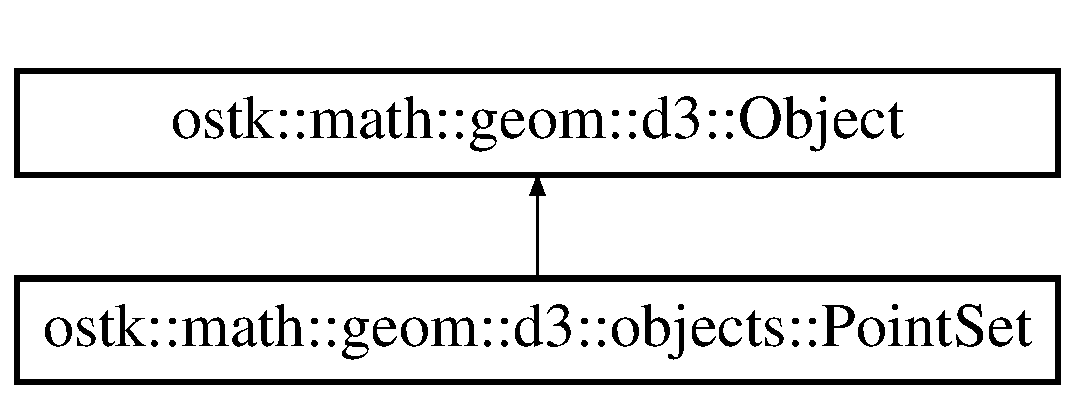
\includegraphics[height=2.000000cm]{classostk_1_1math_1_1geom_1_1d3_1_1objects_1_1_point_set}
\end{center}
\end{figure}
\subsection*{Classes}
\begin{DoxyCompactItemize}
\item 
struct \hyperlink{structostk_1_1math_1_1geom_1_1d3_1_1objects_1_1_point_set_1_1_hasher}{Hasher}
\begin{DoxyCompactList}\small\item\em \hyperlink{classostk_1_1math_1_1geom_1_1d3_1_1objects_1_1_point}{Point} hasher. \end{DoxyCompactList}\end{DoxyCompactItemize}
\subsection*{Public Types}
\begin{DoxyCompactItemize}
\item 
typedef std\+::unordered\+\_\+set$<$ \hyperlink{classostk_1_1math_1_1geom_1_1d3_1_1objects_1_1_point}{Point}, \hyperlink{structostk_1_1math_1_1geom_1_1d3_1_1objects_1_1_point_set_1_1_hasher}{Point\+Set\+::\+Hasher} $>$ \hyperlink{classostk_1_1math_1_1geom_1_1d3_1_1objects_1_1_point_set_a68a2ddeec07bd422601f60d5ed48e183}{Container}
\item 
typedef Point\+Set\+::\+Container\+::const\+\_\+iterator \hyperlink{classostk_1_1math_1_1geom_1_1d3_1_1objects_1_1_point_set_aa87eb9a571cb8b420e8c404005a2b723}{Const\+Iterator}
\end{DoxyCompactItemize}
\subsection*{Public Member Functions}
\begin{DoxyCompactItemize}
\item 
\hyperlink{classostk_1_1math_1_1geom_1_1d3_1_1objects_1_1_point_set_a285835d8348a60ceaf227bd76e3a5546}{Point\+Set} (const Array$<$ \hyperlink{classostk_1_1math_1_1geom_1_1d3_1_1objects_1_1_point}{Point} $>$ \&a\+Point\+Array)
\begin{DoxyCompactList}\small\item\em Constructor. \end{DoxyCompactList}\item 
virtual \hyperlink{classostk_1_1math_1_1geom_1_1d3_1_1objects_1_1_point_set}{Point\+Set} $\ast$ \hyperlink{classostk_1_1math_1_1geom_1_1d3_1_1objects_1_1_point_set_a5936e0dbba4443f938d074c5e77fdac7}{clone} () const override
\begin{DoxyCompactList}\small\item\em Clone point set. \end{DoxyCompactList}\item 
bool \hyperlink{classostk_1_1math_1_1geom_1_1d3_1_1objects_1_1_point_set_a2561f42d2df2e1adf5e6417a2e7e9698}{operator==} (const \hyperlink{classostk_1_1math_1_1geom_1_1d3_1_1objects_1_1_point_set}{Point\+Set} \&a\+Point\+Set) const
\begin{DoxyCompactList}\small\item\em Equal to operator. \end{DoxyCompactList}\item 
bool \hyperlink{classostk_1_1math_1_1geom_1_1d3_1_1objects_1_1_point_set_ae7ac373e11155acfecc8bcfa0b9fde2a}{operator!=} (const \hyperlink{classostk_1_1math_1_1geom_1_1d3_1_1objects_1_1_point_set}{Point\+Set} \&a\+Point\+Set) const
\begin{DoxyCompactList}\small\item\em Not equal to operator. \end{DoxyCompactList}\item 
virtual bool \hyperlink{classostk_1_1math_1_1geom_1_1d3_1_1objects_1_1_point_set_a2457cedb218c01b5f0b16a280ccceb95}{is\+Defined} () const override
\begin{DoxyCompactList}\small\item\em Check if point set is defined. \end{DoxyCompactList}\item 
bool \hyperlink{classostk_1_1math_1_1geom_1_1d3_1_1objects_1_1_point_set_a107e4bdbcee1586d393d804428889049}{is\+Empty} () const
\begin{DoxyCompactList}\small\item\em Check if point set is empty. \end{DoxyCompactList}\item 
bool \hyperlink{classostk_1_1math_1_1geom_1_1d3_1_1objects_1_1_point_set_a5ee3cc0360a12ff12dc960f6a09aacc2}{is\+Near} (const \hyperlink{classostk_1_1math_1_1geom_1_1d3_1_1objects_1_1_point_set}{Point\+Set} \&a\+Point\+Set, const Real \&a\+Tolerance) const
\begin{DoxyCompactList}\small\item\em Check if point set is near another point set. \end{DoxyCompactList}\item 
Size \hyperlink{classostk_1_1math_1_1geom_1_1d3_1_1objects_1_1_point_set_a8c773ea027260feeb3b24298d075f228}{get\+Size} () const
\begin{DoxyCompactList}\small\item\em Get size of point set. \end{DoxyCompactList}\item 
Real \hyperlink{classostk_1_1math_1_1geom_1_1d3_1_1objects_1_1_point_set_ad46f8b9e6d9f9b256fe1d0104f266968}{distance\+To} (const \hyperlink{classostk_1_1math_1_1geom_1_1d3_1_1objects_1_1_point}{Point} \&a\+Point) const
\begin{DoxyCompactList}\small\item\em Get distance to point. \end{DoxyCompactList}\item 
\hyperlink{classostk_1_1math_1_1geom_1_1d3_1_1objects_1_1_point}{Point} \hyperlink{classostk_1_1math_1_1geom_1_1d3_1_1objects_1_1_point_set_a55f63833c4c6fe3481a4f8833701907a}{get\+Point\+Closest\+To} (const \hyperlink{classostk_1_1math_1_1geom_1_1d3_1_1objects_1_1_point}{Point} \&a\+Point) const
\begin{DoxyCompactList}\small\item\em Get point closest to another point. \end{DoxyCompactList}\item 
virtual void \hyperlink{classostk_1_1math_1_1geom_1_1d3_1_1objects_1_1_point_set_adeeac2042e2e518b51c3b8dc4365c130}{print} (std\+::ostream \&an\+Output\+Stream, bool display\+Decorators=true) const override
\begin{DoxyCompactList}\small\item\em Print point. \end{DoxyCompactList}\item 
\hyperlink{classostk_1_1math_1_1geom_1_1d3_1_1objects_1_1_point_set_aa87eb9a571cb8b420e8c404005a2b723}{Point\+Set\+::\+Const\+Iterator} \hyperlink{classostk_1_1math_1_1geom_1_1d3_1_1objects_1_1_point_set_ab660f9c1ab7ec392dce305a0d6cf72a5}{begin} () const
\begin{DoxyCompactList}\small\item\em Get begin const iterator. \end{DoxyCompactList}\item 
\hyperlink{classostk_1_1math_1_1geom_1_1d3_1_1objects_1_1_point_set_aa87eb9a571cb8b420e8c404005a2b723}{Point\+Set\+::\+Const\+Iterator} \hyperlink{classostk_1_1math_1_1geom_1_1d3_1_1objects_1_1_point_set_ad15fd1b2a3609d6e24657118945b579f}{end} () const
\begin{DoxyCompactList}\small\item\em Get end const iterator. \end{DoxyCompactList}\item 
virtual void \hyperlink{classostk_1_1math_1_1geom_1_1d3_1_1objects_1_1_point_set_af03e071aa9d7a364a0c76f563b65a57e}{apply\+Transformation} (const \hyperlink{classostk_1_1math_1_1geom_1_1d3_1_1_transformation}{Transformation} \&a\+Transformation) override
\begin{DoxyCompactList}\small\item\em Apply transformation to point set. \end{DoxyCompactList}\end{DoxyCompactItemize}
\subsection*{Static Public Member Functions}
\begin{DoxyCompactItemize}
\item 
static \hyperlink{classostk_1_1math_1_1geom_1_1d3_1_1objects_1_1_point_set}{Point\+Set} \hyperlink{classostk_1_1math_1_1geom_1_1d3_1_1objects_1_1_point_set_a1b14ed7d73ee7ac5e2796cf44f06ffe9}{Empty} ()
\begin{DoxyCompactList}\small\item\em Constructs an empty point set. \end{DoxyCompactList}\end{DoxyCompactItemize}


\subsection{Detailed Description}
\hyperlink{classostk_1_1math_1_1geom_1_1d3_1_1objects_1_1_point}{Point} set. 

\subsection{Member Typedef Documentation}
\mbox{\Hypertarget{classostk_1_1math_1_1geom_1_1d3_1_1objects_1_1_point_set_aa87eb9a571cb8b420e8c404005a2b723}\label{classostk_1_1math_1_1geom_1_1d3_1_1objects_1_1_point_set_aa87eb9a571cb8b420e8c404005a2b723}} 
\index{ostk\+::math\+::geom\+::d3\+::objects\+::\+Point\+Set@{ostk\+::math\+::geom\+::d3\+::objects\+::\+Point\+Set}!Const\+Iterator@{Const\+Iterator}}
\index{Const\+Iterator@{Const\+Iterator}!ostk\+::math\+::geom\+::d3\+::objects\+::\+Point\+Set@{ostk\+::math\+::geom\+::d3\+::objects\+::\+Point\+Set}}
\subsubsection{\texorpdfstring{Const\+Iterator}{ConstIterator}}
{\footnotesize\ttfamily typedef Point\+Set\+::\+Container\+::const\+\_\+iterator \hyperlink{classostk_1_1math_1_1geom_1_1d3_1_1objects_1_1_point_set_aa87eb9a571cb8b420e8c404005a2b723}{ostk\+::math\+::geom\+::d3\+::objects\+::\+Point\+Set\+::\+Const\+Iterator}}

\mbox{\Hypertarget{classostk_1_1math_1_1geom_1_1d3_1_1objects_1_1_point_set_a68a2ddeec07bd422601f60d5ed48e183}\label{classostk_1_1math_1_1geom_1_1d3_1_1objects_1_1_point_set_a68a2ddeec07bd422601f60d5ed48e183}} 
\index{ostk\+::math\+::geom\+::d3\+::objects\+::\+Point\+Set@{ostk\+::math\+::geom\+::d3\+::objects\+::\+Point\+Set}!Container@{Container}}
\index{Container@{Container}!ostk\+::math\+::geom\+::d3\+::objects\+::\+Point\+Set@{ostk\+::math\+::geom\+::d3\+::objects\+::\+Point\+Set}}
\subsubsection{\texorpdfstring{Container}{Container}}
{\footnotesize\ttfamily typedef std\+::unordered\+\_\+set$<$\hyperlink{classostk_1_1math_1_1geom_1_1d3_1_1objects_1_1_point}{Point}, \hyperlink{structostk_1_1math_1_1geom_1_1d3_1_1objects_1_1_point_set_1_1_hasher}{Point\+Set\+::\+Hasher}$>$ \hyperlink{classostk_1_1math_1_1geom_1_1d3_1_1objects_1_1_point_set_a68a2ddeec07bd422601f60d5ed48e183}{ostk\+::math\+::geom\+::d3\+::objects\+::\+Point\+Set\+::\+Container}}



\subsection{Constructor \& Destructor Documentation}
\mbox{\Hypertarget{classostk_1_1math_1_1geom_1_1d3_1_1objects_1_1_point_set_a285835d8348a60ceaf227bd76e3a5546}\label{classostk_1_1math_1_1geom_1_1d3_1_1objects_1_1_point_set_a285835d8348a60ceaf227bd76e3a5546}} 
\index{ostk\+::math\+::geom\+::d3\+::objects\+::\+Point\+Set@{ostk\+::math\+::geom\+::d3\+::objects\+::\+Point\+Set}!Point\+Set@{Point\+Set}}
\index{Point\+Set@{Point\+Set}!ostk\+::math\+::geom\+::d3\+::objects\+::\+Point\+Set@{ostk\+::math\+::geom\+::d3\+::objects\+::\+Point\+Set}}
\subsubsection{\texorpdfstring{Point\+Set()}{PointSet()}}
{\footnotesize\ttfamily ostk\+::math\+::geom\+::d3\+::objects\+::\+Point\+Set\+::\+Point\+Set (\begin{DoxyParamCaption}\item[{const Array$<$ \hyperlink{classostk_1_1math_1_1geom_1_1d3_1_1objects_1_1_point}{Point} $>$ \&}]{a\+Point\+Array }\end{DoxyParamCaption})}



Constructor. 


\begin{DoxyCode}
\hyperlink{classostk_1_1math_1_1geom_1_1d3_1_1objects_1_1_point_set_a285835d8348a60ceaf227bd76e3a5546}{PointSet} pointSet(\{ \{ 0.0, 0.0, 0.0 \}, \{ 0.0, 0.0, 1.0 \} \}) ;
\end{DoxyCode}



\begin{DoxyParams}[1]{Parameters}
\mbox{\tt in}  & {\em a\+Point\+Array} & A point array \\
\hline
\end{DoxyParams}


\subsection{Member Function Documentation}
\mbox{\Hypertarget{classostk_1_1math_1_1geom_1_1d3_1_1objects_1_1_point_set_af03e071aa9d7a364a0c76f563b65a57e}\label{classostk_1_1math_1_1geom_1_1d3_1_1objects_1_1_point_set_af03e071aa9d7a364a0c76f563b65a57e}} 
\index{ostk\+::math\+::geom\+::d3\+::objects\+::\+Point\+Set@{ostk\+::math\+::geom\+::d3\+::objects\+::\+Point\+Set}!apply\+Transformation@{apply\+Transformation}}
\index{apply\+Transformation@{apply\+Transformation}!ostk\+::math\+::geom\+::d3\+::objects\+::\+Point\+Set@{ostk\+::math\+::geom\+::d3\+::objects\+::\+Point\+Set}}
\subsubsection{\texorpdfstring{apply\+Transformation()}{applyTransformation()}}
{\footnotesize\ttfamily void ostk\+::math\+::geom\+::d3\+::objects\+::\+Point\+Set\+::apply\+Transformation (\begin{DoxyParamCaption}\item[{const \hyperlink{classostk_1_1math_1_1geom_1_1d3_1_1_transformation}{Transformation} \&}]{a\+Transformation }\end{DoxyParamCaption})\hspace{0.3cm}{\ttfamily [override]}, {\ttfamily [virtual]}}



Apply transformation to point set. 


\begin{DoxyParams}[1]{Parameters}
\mbox{\tt in}  & {\em a\+Transformation} & A transformation \\
\hline
\end{DoxyParams}


Implements \hyperlink{classostk_1_1math_1_1geom_1_1d3_1_1_object_ae9194dd6d2bb4df09292ffc84dccdb1d}{ostk\+::math\+::geom\+::d3\+::\+Object}.

\mbox{\Hypertarget{classostk_1_1math_1_1geom_1_1d3_1_1objects_1_1_point_set_ab660f9c1ab7ec392dce305a0d6cf72a5}\label{classostk_1_1math_1_1geom_1_1d3_1_1objects_1_1_point_set_ab660f9c1ab7ec392dce305a0d6cf72a5}} 
\index{ostk\+::math\+::geom\+::d3\+::objects\+::\+Point\+Set@{ostk\+::math\+::geom\+::d3\+::objects\+::\+Point\+Set}!begin@{begin}}
\index{begin@{begin}!ostk\+::math\+::geom\+::d3\+::objects\+::\+Point\+Set@{ostk\+::math\+::geom\+::d3\+::objects\+::\+Point\+Set}}
\subsubsection{\texorpdfstring{begin()}{begin()}}
{\footnotesize\ttfamily \hyperlink{classostk_1_1math_1_1geom_1_1d3_1_1objects_1_1_point_set_aa87eb9a571cb8b420e8c404005a2b723}{Point\+Set\+::\+Const\+Iterator} ostk\+::math\+::geom\+::d3\+::objects\+::\+Point\+Set\+::begin (\begin{DoxyParamCaption}{ }\end{DoxyParamCaption}) const}



Get begin const iterator. 

\begin{DoxyReturn}{Returns}
Begin const iterator 
\end{DoxyReturn}
\mbox{\Hypertarget{classostk_1_1math_1_1geom_1_1d3_1_1objects_1_1_point_set_a5936e0dbba4443f938d074c5e77fdac7}\label{classostk_1_1math_1_1geom_1_1d3_1_1objects_1_1_point_set_a5936e0dbba4443f938d074c5e77fdac7}} 
\index{ostk\+::math\+::geom\+::d3\+::objects\+::\+Point\+Set@{ostk\+::math\+::geom\+::d3\+::objects\+::\+Point\+Set}!clone@{clone}}
\index{clone@{clone}!ostk\+::math\+::geom\+::d3\+::objects\+::\+Point\+Set@{ostk\+::math\+::geom\+::d3\+::objects\+::\+Point\+Set}}
\subsubsection{\texorpdfstring{clone()}{clone()}}
{\footnotesize\ttfamily \hyperlink{classostk_1_1math_1_1geom_1_1d3_1_1objects_1_1_point_set}{Point\+Set} $\ast$ ostk\+::math\+::geom\+::d3\+::objects\+::\+Point\+Set\+::clone (\begin{DoxyParamCaption}{ }\end{DoxyParamCaption}) const\hspace{0.3cm}{\ttfamily [override]}, {\ttfamily [virtual]}}



Clone point set. 

\begin{DoxyReturn}{Returns}
Pointer to cloned point set 
\end{DoxyReturn}


Implements \hyperlink{classostk_1_1math_1_1geom_1_1d3_1_1_object_a676013f9555f6492687f9809b2db887b}{ostk\+::math\+::geom\+::d3\+::\+Object}.

\mbox{\Hypertarget{classostk_1_1math_1_1geom_1_1d3_1_1objects_1_1_point_set_ad46f8b9e6d9f9b256fe1d0104f266968}\label{classostk_1_1math_1_1geom_1_1d3_1_1objects_1_1_point_set_ad46f8b9e6d9f9b256fe1d0104f266968}} 
\index{ostk\+::math\+::geom\+::d3\+::objects\+::\+Point\+Set@{ostk\+::math\+::geom\+::d3\+::objects\+::\+Point\+Set}!distance\+To@{distance\+To}}
\index{distance\+To@{distance\+To}!ostk\+::math\+::geom\+::d3\+::objects\+::\+Point\+Set@{ostk\+::math\+::geom\+::d3\+::objects\+::\+Point\+Set}}
\subsubsection{\texorpdfstring{distance\+To()}{distanceTo()}}
{\footnotesize\ttfamily Real ostk\+::math\+::geom\+::d3\+::objects\+::\+Point\+Set\+::distance\+To (\begin{DoxyParamCaption}\item[{const \hyperlink{classostk_1_1math_1_1geom_1_1d3_1_1objects_1_1_point}{Point} \&}]{a\+Point }\end{DoxyParamCaption}) const}



Get distance to point. 


\begin{DoxyParams}[1]{Parameters}
\mbox{\tt in}  & {\em a\+Point} & A point \\
\hline
\end{DoxyParams}
\begin{DoxyReturn}{Returns}
Distance to point 
\end{DoxyReturn}
\mbox{\Hypertarget{classostk_1_1math_1_1geom_1_1d3_1_1objects_1_1_point_set_a1b14ed7d73ee7ac5e2796cf44f06ffe9}\label{classostk_1_1math_1_1geom_1_1d3_1_1objects_1_1_point_set_a1b14ed7d73ee7ac5e2796cf44f06ffe9}} 
\index{ostk\+::math\+::geom\+::d3\+::objects\+::\+Point\+Set@{ostk\+::math\+::geom\+::d3\+::objects\+::\+Point\+Set}!Empty@{Empty}}
\index{Empty@{Empty}!ostk\+::math\+::geom\+::d3\+::objects\+::\+Point\+Set@{ostk\+::math\+::geom\+::d3\+::objects\+::\+Point\+Set}}
\subsubsection{\texorpdfstring{Empty()}{Empty()}}
{\footnotesize\ttfamily \hyperlink{classostk_1_1math_1_1geom_1_1d3_1_1objects_1_1_point_set}{Point\+Set} ostk\+::math\+::geom\+::d3\+::objects\+::\+Point\+Set\+::\+Empty (\begin{DoxyParamCaption}{ }\end{DoxyParamCaption})\hspace{0.3cm}{\ttfamily [static]}}



Constructs an empty point set. 


\begin{DoxyCode}
\hyperlink{classostk_1_1math_1_1geom_1_1d3_1_1objects_1_1_point_set_a285835d8348a60ceaf227bd76e3a5546}{PointSet} pointSet = \hyperlink{classostk_1_1math_1_1geom_1_1d3_1_1objects_1_1_point_set_a1b14ed7d73ee7ac5e2796cf44f06ffe9}{PointSet::Empty}() ;
\end{DoxyCode}


\begin{DoxyReturn}{Returns}
Empty point set 
\end{DoxyReturn}
\mbox{\Hypertarget{classostk_1_1math_1_1geom_1_1d3_1_1objects_1_1_point_set_ad15fd1b2a3609d6e24657118945b579f}\label{classostk_1_1math_1_1geom_1_1d3_1_1objects_1_1_point_set_ad15fd1b2a3609d6e24657118945b579f}} 
\index{ostk\+::math\+::geom\+::d3\+::objects\+::\+Point\+Set@{ostk\+::math\+::geom\+::d3\+::objects\+::\+Point\+Set}!end@{end}}
\index{end@{end}!ostk\+::math\+::geom\+::d3\+::objects\+::\+Point\+Set@{ostk\+::math\+::geom\+::d3\+::objects\+::\+Point\+Set}}
\subsubsection{\texorpdfstring{end()}{end()}}
{\footnotesize\ttfamily \hyperlink{classostk_1_1math_1_1geom_1_1d3_1_1objects_1_1_point_set_aa87eb9a571cb8b420e8c404005a2b723}{Point\+Set\+::\+Const\+Iterator} ostk\+::math\+::geom\+::d3\+::objects\+::\+Point\+Set\+::end (\begin{DoxyParamCaption}{ }\end{DoxyParamCaption}) const}



Get end const iterator. 

\begin{DoxyReturn}{Returns}
End const iterator 
\end{DoxyReturn}
\mbox{\Hypertarget{classostk_1_1math_1_1geom_1_1d3_1_1objects_1_1_point_set_a55f63833c4c6fe3481a4f8833701907a}\label{classostk_1_1math_1_1geom_1_1d3_1_1objects_1_1_point_set_a55f63833c4c6fe3481a4f8833701907a}} 
\index{ostk\+::math\+::geom\+::d3\+::objects\+::\+Point\+Set@{ostk\+::math\+::geom\+::d3\+::objects\+::\+Point\+Set}!get\+Point\+Closest\+To@{get\+Point\+Closest\+To}}
\index{get\+Point\+Closest\+To@{get\+Point\+Closest\+To}!ostk\+::math\+::geom\+::d3\+::objects\+::\+Point\+Set@{ostk\+::math\+::geom\+::d3\+::objects\+::\+Point\+Set}}
\subsubsection{\texorpdfstring{get\+Point\+Closest\+To()}{getPointClosestTo()}}
{\footnotesize\ttfamily \hyperlink{classostk_1_1math_1_1geom_1_1d3_1_1objects_1_1_point}{Point} ostk\+::math\+::geom\+::d3\+::objects\+::\+Point\+Set\+::get\+Point\+Closest\+To (\begin{DoxyParamCaption}\item[{const \hyperlink{classostk_1_1math_1_1geom_1_1d3_1_1objects_1_1_point}{Point} \&}]{a\+Point }\end{DoxyParamCaption}) const}



Get point closest to another point. 


\begin{DoxyParams}[1]{Parameters}
\mbox{\tt in}  & {\em a\+Point} & A point \\
\hline
\end{DoxyParams}
\begin{DoxyReturn}{Returns}
Closest point 
\end{DoxyReturn}
\mbox{\Hypertarget{classostk_1_1math_1_1geom_1_1d3_1_1objects_1_1_point_set_a8c773ea027260feeb3b24298d075f228}\label{classostk_1_1math_1_1geom_1_1d3_1_1objects_1_1_point_set_a8c773ea027260feeb3b24298d075f228}} 
\index{ostk\+::math\+::geom\+::d3\+::objects\+::\+Point\+Set@{ostk\+::math\+::geom\+::d3\+::objects\+::\+Point\+Set}!get\+Size@{get\+Size}}
\index{get\+Size@{get\+Size}!ostk\+::math\+::geom\+::d3\+::objects\+::\+Point\+Set@{ostk\+::math\+::geom\+::d3\+::objects\+::\+Point\+Set}}
\subsubsection{\texorpdfstring{get\+Size()}{getSize()}}
{\footnotesize\ttfamily Size ostk\+::math\+::geom\+::d3\+::objects\+::\+Point\+Set\+::get\+Size (\begin{DoxyParamCaption}{ }\end{DoxyParamCaption}) const}



Get size of point set. 

\begin{DoxyReturn}{Returns}
Size of point set 
\end{DoxyReturn}
\mbox{\Hypertarget{classostk_1_1math_1_1geom_1_1d3_1_1objects_1_1_point_set_a2457cedb218c01b5f0b16a280ccceb95}\label{classostk_1_1math_1_1geom_1_1d3_1_1objects_1_1_point_set_a2457cedb218c01b5f0b16a280ccceb95}} 
\index{ostk\+::math\+::geom\+::d3\+::objects\+::\+Point\+Set@{ostk\+::math\+::geom\+::d3\+::objects\+::\+Point\+Set}!is\+Defined@{is\+Defined}}
\index{is\+Defined@{is\+Defined}!ostk\+::math\+::geom\+::d3\+::objects\+::\+Point\+Set@{ostk\+::math\+::geom\+::d3\+::objects\+::\+Point\+Set}}
\subsubsection{\texorpdfstring{is\+Defined()}{isDefined()}}
{\footnotesize\ttfamily bool ostk\+::math\+::geom\+::d3\+::objects\+::\+Point\+Set\+::is\+Defined (\begin{DoxyParamCaption}{ }\end{DoxyParamCaption}) const\hspace{0.3cm}{\ttfamily [override]}, {\ttfamily [virtual]}}



Check if point set is defined. 


\begin{DoxyCode}
\hyperlink{classostk_1_1math_1_1geom_1_1d3_1_1objects_1_1_point_set_a285835d8348a60ceaf227bd76e3a5546}{PointSet}(0.0, 0.0, 0.0).isDefined() ; \textcolor{comment}{// True}
\end{DoxyCode}


\begin{DoxyReturn}{Returns}
True if point set is defined 
\end{DoxyReturn}


Implements \hyperlink{classostk_1_1math_1_1geom_1_1d3_1_1_object_a271a1964cd208be85ce9a0a429395ad8}{ostk\+::math\+::geom\+::d3\+::\+Object}.

\mbox{\Hypertarget{classostk_1_1math_1_1geom_1_1d3_1_1objects_1_1_point_set_a107e4bdbcee1586d393d804428889049}\label{classostk_1_1math_1_1geom_1_1d3_1_1objects_1_1_point_set_a107e4bdbcee1586d393d804428889049}} 
\index{ostk\+::math\+::geom\+::d3\+::objects\+::\+Point\+Set@{ostk\+::math\+::geom\+::d3\+::objects\+::\+Point\+Set}!is\+Empty@{is\+Empty}}
\index{is\+Empty@{is\+Empty}!ostk\+::math\+::geom\+::d3\+::objects\+::\+Point\+Set@{ostk\+::math\+::geom\+::d3\+::objects\+::\+Point\+Set}}
\subsubsection{\texorpdfstring{is\+Empty()}{isEmpty()}}
{\footnotesize\ttfamily bool ostk\+::math\+::geom\+::d3\+::objects\+::\+Point\+Set\+::is\+Empty (\begin{DoxyParamCaption}{ }\end{DoxyParamCaption}) const}



Check if point set is empty. 


\begin{DoxyCode}
\hyperlink{classostk_1_1math_1_1geom_1_1d3_1_1objects_1_1_point_set_a1b14ed7d73ee7ac5e2796cf44f06ffe9}{PointSet::Empty}().\hyperlink{classostk_1_1math_1_1geom_1_1d3_1_1objects_1_1_point_set_a107e4bdbcee1586d393d804428889049}{isEmpty}() ; \textcolor{comment}{// True}
\end{DoxyCode}


\begin{DoxyReturn}{Returns}
True if point set is empty 
\end{DoxyReturn}
\mbox{\Hypertarget{classostk_1_1math_1_1geom_1_1d3_1_1objects_1_1_point_set_a5ee3cc0360a12ff12dc960f6a09aacc2}\label{classostk_1_1math_1_1geom_1_1d3_1_1objects_1_1_point_set_a5ee3cc0360a12ff12dc960f6a09aacc2}} 
\index{ostk\+::math\+::geom\+::d3\+::objects\+::\+Point\+Set@{ostk\+::math\+::geom\+::d3\+::objects\+::\+Point\+Set}!is\+Near@{is\+Near}}
\index{is\+Near@{is\+Near}!ostk\+::math\+::geom\+::d3\+::objects\+::\+Point\+Set@{ostk\+::math\+::geom\+::d3\+::objects\+::\+Point\+Set}}
\subsubsection{\texorpdfstring{is\+Near()}{isNear()}}
{\footnotesize\ttfamily bool ostk\+::math\+::geom\+::d3\+::objects\+::\+Point\+Set\+::is\+Near (\begin{DoxyParamCaption}\item[{const \hyperlink{classostk_1_1math_1_1geom_1_1d3_1_1objects_1_1_point_set}{Point\+Set} \&}]{a\+Point\+Set,  }\item[{const Real \&}]{a\+Tolerance }\end{DoxyParamCaption}) const}



Check if point set is near another point set. 


\begin{DoxyCode}
\hyperlink{classostk_1_1math_1_1geom_1_1d3_1_1objects_1_1_point_set_a285835d8348a60ceaf227bd76e3a5546}{PointSet}(\{ \{ 0.0, 0.0, 0.0 \}, \{ 0.0, 0.0, 1.0 \} \}).\hyperlink{classostk_1_1math_1_1geom_1_1d3_1_1objects_1_1_point_set_a5ee3cc0360a12ff12dc960f6a09aacc2}{isNear}(\hyperlink{classostk_1_1math_1_1geom_1_1d3_1_1objects_1_1_point_set_a285835d8348a60ceaf227bd76e3a5546}{PointSet}(\{ \{ 0.0, 1e-15, 0.
      0 \}, \{ 0.0, 0.0, 1.0 \} \}), 1e-15) ; \textcolor{comment}{// True}
\end{DoxyCode}



\begin{DoxyParams}[1]{Parameters}
\mbox{\tt in}  & {\em a\+Point\+Set} & A point set \\
\hline
\mbox{\tt in}  & {\em a\+Tolerance} & A tolerance \\
\hline
\end{DoxyParams}
\begin{DoxyReturn}{Returns}
True if point set is near another point set 
\end{DoxyReturn}
\mbox{\Hypertarget{classostk_1_1math_1_1geom_1_1d3_1_1objects_1_1_point_set_ae7ac373e11155acfecc8bcfa0b9fde2a}\label{classostk_1_1math_1_1geom_1_1d3_1_1objects_1_1_point_set_ae7ac373e11155acfecc8bcfa0b9fde2a}} 
\index{ostk\+::math\+::geom\+::d3\+::objects\+::\+Point\+Set@{ostk\+::math\+::geom\+::d3\+::objects\+::\+Point\+Set}!operator"!=@{operator"!=}}
\index{operator"!=@{operator"!=}!ostk\+::math\+::geom\+::d3\+::objects\+::\+Point\+Set@{ostk\+::math\+::geom\+::d3\+::objects\+::\+Point\+Set}}
\subsubsection{\texorpdfstring{operator"!=()}{operator!=()}}
{\footnotesize\ttfamily bool ostk\+::math\+::geom\+::d3\+::objects\+::\+Point\+Set\+::operator!= (\begin{DoxyParamCaption}\item[{const \hyperlink{classostk_1_1math_1_1geom_1_1d3_1_1objects_1_1_point_set}{Point\+Set} \&}]{a\+Point\+Set }\end{DoxyParamCaption}) const}



Not equal to operator. 


\begin{DoxyParams}[1]{Parameters}
\mbox{\tt in}  & {\em a\+Point\+Set} & A point set \\
\hline
\end{DoxyParams}
\begin{DoxyReturn}{Returns}
True if point sets are not equal 
\end{DoxyReturn}
\mbox{\Hypertarget{classostk_1_1math_1_1geom_1_1d3_1_1objects_1_1_point_set_a2561f42d2df2e1adf5e6417a2e7e9698}\label{classostk_1_1math_1_1geom_1_1d3_1_1objects_1_1_point_set_a2561f42d2df2e1adf5e6417a2e7e9698}} 
\index{ostk\+::math\+::geom\+::d3\+::objects\+::\+Point\+Set@{ostk\+::math\+::geom\+::d3\+::objects\+::\+Point\+Set}!operator==@{operator==}}
\index{operator==@{operator==}!ostk\+::math\+::geom\+::d3\+::objects\+::\+Point\+Set@{ostk\+::math\+::geom\+::d3\+::objects\+::\+Point\+Set}}
\subsubsection{\texorpdfstring{operator==()}{operator==()}}
{\footnotesize\ttfamily bool ostk\+::math\+::geom\+::d3\+::objects\+::\+Point\+Set\+::operator== (\begin{DoxyParamCaption}\item[{const \hyperlink{classostk_1_1math_1_1geom_1_1d3_1_1objects_1_1_point_set}{Point\+Set} \&}]{a\+Point\+Set }\end{DoxyParamCaption}) const}



Equal to operator. 


\begin{DoxyParams}[1]{Parameters}
\mbox{\tt in}  & {\em a\+Point\+Set} & A point set \\
\hline
\end{DoxyParams}
\begin{DoxyReturn}{Returns}
True if point sets are equal 
\end{DoxyReturn}
\mbox{\Hypertarget{classostk_1_1math_1_1geom_1_1d3_1_1objects_1_1_point_set_adeeac2042e2e518b51c3b8dc4365c130}\label{classostk_1_1math_1_1geom_1_1d3_1_1objects_1_1_point_set_adeeac2042e2e518b51c3b8dc4365c130}} 
\index{ostk\+::math\+::geom\+::d3\+::objects\+::\+Point\+Set@{ostk\+::math\+::geom\+::d3\+::objects\+::\+Point\+Set}!print@{print}}
\index{print@{print}!ostk\+::math\+::geom\+::d3\+::objects\+::\+Point\+Set@{ostk\+::math\+::geom\+::d3\+::objects\+::\+Point\+Set}}
\subsubsection{\texorpdfstring{print()}{print()}}
{\footnotesize\ttfamily void ostk\+::math\+::geom\+::d3\+::objects\+::\+Point\+Set\+::print (\begin{DoxyParamCaption}\item[{std\+::ostream \&}]{an\+Output\+Stream,  }\item[{bool}]{display\+Decorators = {\ttfamily true} }\end{DoxyParamCaption}) const\hspace{0.3cm}{\ttfamily [override]}, {\ttfamily [virtual]}}



Print point. 


\begin{DoxyParams}[1]{Parameters}
\mbox{\tt in}  & {\em an\+Output\+Stream} & An output stream \\
\hline
\mbox{\tt in}  & {\em (optional)} & display\+Decorators If true, display decorators \\
\hline
\end{DoxyParams}


Implements \hyperlink{classostk_1_1math_1_1geom_1_1d3_1_1_object_ab2a2a782503b97d1cecabdfedc636fce}{ostk\+::math\+::geom\+::d3\+::\+Object}.



The documentation for this class was generated from the following files\+:\begin{DoxyCompactItemize}
\item 
include/\+Open\+Space\+Toolkit/\+Mathematics/\+Geometry/3\+D/\+Objects/\hyperlink{3_d_2_objects_2_point_set_8hpp}{Point\+Set.\+hpp}\item 
src/\+Open\+Space\+Toolkit/\+Mathematics/\+Geometry/3\+D/\+Objects/\hyperlink{3_d_2_objects_2_point_set_8cpp}{Point\+Set.\+cpp}\end{DoxyCompactItemize}

\hypertarget{classostk_1_1math_1_1geom_1_1d2_1_1objects_1_1_point_set}{}\doxysection{ostk\+::math\+::geom\+::d2\+::objects\+::Point\+Set Class Reference}
\label{classostk_1_1math_1_1geom_1_1d2_1_1objects_1_1_point_set}\index{ostk::math::geom::d2::objects::PointSet@{ostk::math::geom::d2::objects::PointSet}}


\mbox{\hyperlink{classostk_1_1math_1_1geom_1_1d2_1_1objects_1_1_point}{Point}} set.  




{\ttfamily \#include $<$Point\+Set.\+hpp$>$}

Inheritance diagram for ostk\+::math\+::geom\+::d2\+::objects\+::Point\+Set\+:\begin{figure}[H]
\begin{center}
\leavevmode
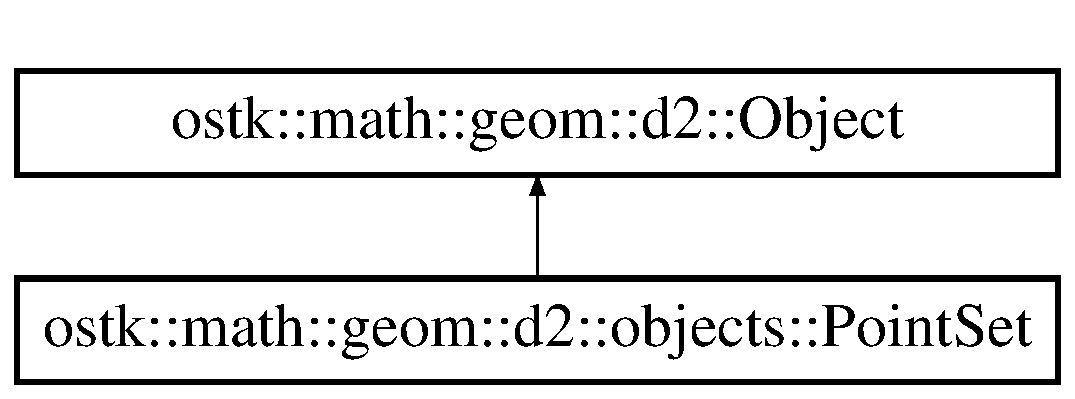
\includegraphics[height=2.000000cm]{classostk_1_1math_1_1geom_1_1d2_1_1objects_1_1_point_set}
\end{center}
\end{figure}
\doxysubsection*{Classes}
\begin{DoxyCompactItemize}
\item 
struct \mbox{\hyperlink{structostk_1_1math_1_1geom_1_1d2_1_1objects_1_1_point_set_1_1_hasher}{Hasher}}
\begin{DoxyCompactList}\small\item\em \mbox{\hyperlink{classostk_1_1math_1_1geom_1_1d2_1_1objects_1_1_point}{Point}} hasher. \end{DoxyCompactList}\end{DoxyCompactItemize}
\doxysubsection*{Public Types}
\begin{DoxyCompactItemize}
\item 
typedef std\+::unordered\+\_\+set$<$ \mbox{\hyperlink{classostk_1_1math_1_1geom_1_1d2_1_1objects_1_1_point}{Point}}, \mbox{\hyperlink{structostk_1_1math_1_1geom_1_1d2_1_1objects_1_1_point_set_1_1_hasher}{Point\+Set\+::\+Hasher}} $>$ \mbox{\hyperlink{classostk_1_1math_1_1geom_1_1d2_1_1objects_1_1_point_set_ac65ec2015127166d3aa98b163e2a7199}{Container}}
\item 
typedef Point\+Set\+::\+Container\+::const\+\_\+iterator \mbox{\hyperlink{classostk_1_1math_1_1geom_1_1d2_1_1objects_1_1_point_set_a6a0613cc686e9247430658eee91036d0}{Const\+Iterator}}
\end{DoxyCompactItemize}
\doxysubsection*{Public Member Functions}
\begin{DoxyCompactItemize}
\item 
\mbox{\hyperlink{classostk_1_1math_1_1geom_1_1d2_1_1objects_1_1_point_set_a736eff7b0d1c876b304bfa7d1d2d0095}{Point\+Set}} (const Array$<$ \mbox{\hyperlink{classostk_1_1math_1_1geom_1_1d2_1_1objects_1_1_point}{Point}} $>$ \&a\+Point\+Array)
\begin{DoxyCompactList}\small\item\em Constructor. \end{DoxyCompactList}\item 
virtual \mbox{\hyperlink{classostk_1_1math_1_1geom_1_1d2_1_1objects_1_1_point_set}{Point\+Set}} $\ast$ \mbox{\hyperlink{classostk_1_1math_1_1geom_1_1d2_1_1objects_1_1_point_set_ac1d1c3727df0f10f527aa3d3551c8f4e}{clone}} () const override
\begin{DoxyCompactList}\small\item\em Clone point set. \end{DoxyCompactList}\item 
bool \mbox{\hyperlink{classostk_1_1math_1_1geom_1_1d2_1_1objects_1_1_point_set_adab3ff08c4e5413822f35408be2f2ec1}{operator==}} (const \mbox{\hyperlink{classostk_1_1math_1_1geom_1_1d2_1_1objects_1_1_point_set}{Point\+Set}} \&a\+Point\+Set) const
\begin{DoxyCompactList}\small\item\em Equal to operator. \end{DoxyCompactList}\item 
bool \mbox{\hyperlink{classostk_1_1math_1_1geom_1_1d2_1_1objects_1_1_point_set_a39cd3a4723640724737624d9aded01bd}{operator!=}} (const \mbox{\hyperlink{classostk_1_1math_1_1geom_1_1d2_1_1objects_1_1_point_set}{Point\+Set}} \&a\+Point\+Set) const
\begin{DoxyCompactList}\small\item\em Not equal to operator. \end{DoxyCompactList}\item 
virtual bool \mbox{\hyperlink{classostk_1_1math_1_1geom_1_1d2_1_1objects_1_1_point_set_a6b2dd586eeb7f4fbf659fa9810574315}{is\+Defined}} () const override
\begin{DoxyCompactList}\small\item\em Check if point set is defined. \end{DoxyCompactList}\item 
bool \mbox{\hyperlink{classostk_1_1math_1_1geom_1_1d2_1_1objects_1_1_point_set_a1df6b975efcbfc495dbdc947dc632846}{is\+Empty}} () const
\begin{DoxyCompactList}\small\item\em Check if point set is empty. \end{DoxyCompactList}\item 
bool \mbox{\hyperlink{classostk_1_1math_1_1geom_1_1d2_1_1objects_1_1_point_set_ab11988a5a567985298249b3e8d30842b}{is\+Near}} (const \mbox{\hyperlink{classostk_1_1math_1_1geom_1_1d2_1_1objects_1_1_point_set}{Point\+Set}} \&a\+Point\+Set, const Real \&a\+Tolerance) const
\begin{DoxyCompactList}\small\item\em Check if point set is near another point set. \end{DoxyCompactList}\item 
Size \mbox{\hyperlink{classostk_1_1math_1_1geom_1_1d2_1_1objects_1_1_point_set_a169dfd11b6bd2e162f1ceb632ee19508}{get\+Size}} () const
\begin{DoxyCompactList}\small\item\em Get size of point set. \end{DoxyCompactList}\item 
Real \mbox{\hyperlink{classostk_1_1math_1_1geom_1_1d2_1_1objects_1_1_point_set_a3d5dd5bed603fd73b8f0e8eeaeb48693}{distance\+To}} (const \mbox{\hyperlink{classostk_1_1math_1_1geom_1_1d2_1_1objects_1_1_point}{Point}} \&a\+Point) const
\begin{DoxyCompactList}\small\item\em Get distance to point. \end{DoxyCompactList}\item 
\mbox{\hyperlink{classostk_1_1math_1_1geom_1_1d2_1_1objects_1_1_point}{Point}} \mbox{\hyperlink{classostk_1_1math_1_1geom_1_1d2_1_1objects_1_1_point_set_a1d08aa1b16ad2865f09a25267c63e58b}{get\+Point\+Closest\+To}} (const \mbox{\hyperlink{classostk_1_1math_1_1geom_1_1d2_1_1objects_1_1_point}{Point}} \&a\+Point) const
\begin{DoxyCompactList}\small\item\em Get point closest to another point. \end{DoxyCompactList}\item 
virtual String \mbox{\hyperlink{classostk_1_1math_1_1geom_1_1d2_1_1objects_1_1_point_set_af032e86d9d9dcabe229a015a8361daf2}{to\+String}} (const \mbox{\hyperlink{classostk_1_1math_1_1geom_1_1d2_1_1_object_aa76f9e30caebf4005bafbdff447f66cf}{Object\+::\+Format}} \&a\+Format=\mbox{\hyperlink{classostk_1_1math_1_1geom_1_1d2_1_1_object_aa76f9e30caebf4005bafbdff447f66cfaeb6d8ae6f20283755b339c0dc273988b}{Object\+::\+Format\+::\+Standard}}, const Integer \&a\+Precision=Integer\+::\+Undefined()) const override
\begin{DoxyCompactList}\small\item\em Get string representation. \end{DoxyCompactList}\item 
virtual void \mbox{\hyperlink{classostk_1_1math_1_1geom_1_1d2_1_1objects_1_1_point_set_aef3263b63b2e9c9667365f58faee9ac7}{print}} (std\+::ostream \&an\+Output\+Stream, bool display\+Decorators=true) const override
\begin{DoxyCompactList}\small\item\em Print point. \end{DoxyCompactList}\item 
\mbox{\hyperlink{classostk_1_1math_1_1geom_1_1d2_1_1objects_1_1_point_set_a6a0613cc686e9247430658eee91036d0}{Point\+Set\+::\+Const\+Iterator}} \mbox{\hyperlink{classostk_1_1math_1_1geom_1_1d2_1_1objects_1_1_point_set_aaa290d13737a148694f97fc557e2069a}{begin}} () const
\begin{DoxyCompactList}\small\item\em Get begin const iterator. \end{DoxyCompactList}\item 
\mbox{\hyperlink{classostk_1_1math_1_1geom_1_1d2_1_1objects_1_1_point_set_a6a0613cc686e9247430658eee91036d0}{Point\+Set\+::\+Const\+Iterator}} \mbox{\hyperlink{classostk_1_1math_1_1geom_1_1d2_1_1objects_1_1_point_set_a49b262b5d0e453fd1870cce164b7288d}{end}} () const
\begin{DoxyCompactList}\small\item\em Get end const iterator. \end{DoxyCompactList}\item 
virtual void \mbox{\hyperlink{classostk_1_1math_1_1geom_1_1d2_1_1objects_1_1_point_set_a8c4140ca8434580a95df773d3aeed5bb}{apply\+Transformation}} (const \mbox{\hyperlink{classostk_1_1math_1_1geom_1_1d2_1_1_transformation}{Transformation}} \&a\+Transformation) override
\begin{DoxyCompactList}\small\item\em Apply transformation to point set. \end{DoxyCompactList}\end{DoxyCompactItemize}
\doxysubsection*{Static Public Member Functions}
\begin{DoxyCompactItemize}
\item 
static \mbox{\hyperlink{classostk_1_1math_1_1geom_1_1d2_1_1objects_1_1_point_set}{Point\+Set}} \mbox{\hyperlink{classostk_1_1math_1_1geom_1_1d2_1_1objects_1_1_point_set_a09f5e125c7b4545a75e4eea6193bf615}{Empty}} ()
\begin{DoxyCompactList}\small\item\em Constructs an empty point set. \end{DoxyCompactList}\end{DoxyCompactItemize}


\doxysubsection{Detailed Description}
\mbox{\hyperlink{classostk_1_1math_1_1geom_1_1d2_1_1objects_1_1_point}{Point}} set. 

\doxysubsection{Member Typedef Documentation}
\mbox{\Hypertarget{classostk_1_1math_1_1geom_1_1d2_1_1objects_1_1_point_set_a6a0613cc686e9247430658eee91036d0}\label{classostk_1_1math_1_1geom_1_1d2_1_1objects_1_1_point_set_a6a0613cc686e9247430658eee91036d0}} 
\index{ostk::math::geom::d2::objects::PointSet@{ostk::math::geom::d2::objects::PointSet}!ConstIterator@{ConstIterator}}
\index{ConstIterator@{ConstIterator}!ostk::math::geom::d2::objects::PointSet@{ostk::math::geom::d2::objects::PointSet}}
\doxysubsubsection{\texorpdfstring{ConstIterator}{ConstIterator}}
{\footnotesize\ttfamily typedef Point\+Set\+::\+Container\+::const\+\_\+iterator \mbox{\hyperlink{classostk_1_1math_1_1geom_1_1d2_1_1objects_1_1_point_set_a6a0613cc686e9247430658eee91036d0}{ostk\+::math\+::geom\+::d2\+::objects\+::\+Point\+Set\+::\+Const\+Iterator}}}

\mbox{\Hypertarget{classostk_1_1math_1_1geom_1_1d2_1_1objects_1_1_point_set_ac65ec2015127166d3aa98b163e2a7199}\label{classostk_1_1math_1_1geom_1_1d2_1_1objects_1_1_point_set_ac65ec2015127166d3aa98b163e2a7199}} 
\index{ostk::math::geom::d2::objects::PointSet@{ostk::math::geom::d2::objects::PointSet}!Container@{Container}}
\index{Container@{Container}!ostk::math::geom::d2::objects::PointSet@{ostk::math::geom::d2::objects::PointSet}}
\doxysubsubsection{\texorpdfstring{Container}{Container}}
{\footnotesize\ttfamily typedef std\+::unordered\+\_\+set$<$\mbox{\hyperlink{classostk_1_1math_1_1geom_1_1d2_1_1objects_1_1_point}{Point}}, \mbox{\hyperlink{structostk_1_1math_1_1geom_1_1d2_1_1objects_1_1_point_set_1_1_hasher}{Point\+Set\+::\+Hasher}}$>$ \mbox{\hyperlink{classostk_1_1math_1_1geom_1_1d2_1_1objects_1_1_point_set_ac65ec2015127166d3aa98b163e2a7199}{ostk\+::math\+::geom\+::d2\+::objects\+::\+Point\+Set\+::\+Container}}}



\doxysubsection{Constructor \& Destructor Documentation}
\mbox{\Hypertarget{classostk_1_1math_1_1geom_1_1d2_1_1objects_1_1_point_set_a736eff7b0d1c876b304bfa7d1d2d0095}\label{classostk_1_1math_1_1geom_1_1d2_1_1objects_1_1_point_set_a736eff7b0d1c876b304bfa7d1d2d0095}} 
\index{ostk::math::geom::d2::objects::PointSet@{ostk::math::geom::d2::objects::PointSet}!PointSet@{PointSet}}
\index{PointSet@{PointSet}!ostk::math::geom::d2::objects::PointSet@{ostk::math::geom::d2::objects::PointSet}}
\doxysubsubsection{\texorpdfstring{PointSet()}{PointSet()}}
{\footnotesize\ttfamily ostk\+::math\+::geom\+::d2\+::objects\+::\+Point\+Set\+::\+Point\+Set (\begin{DoxyParamCaption}\item[{const Array$<$ \mbox{\hyperlink{classostk_1_1math_1_1geom_1_1d2_1_1objects_1_1_point}{Point}} $>$ \&}]{a\+Point\+Array }\end{DoxyParamCaption})}



Constructor. 


\begin{DoxyCode}{0}
\DoxyCodeLine{\mbox{\hyperlink{classostk_1_1math_1_1geom_1_1d2_1_1objects_1_1_point_set_a736eff7b0d1c876b304bfa7d1d2d0095}{PointSet}} pointSet(\{ \{ 0.0, 0.0 \}, \{ 0.0, 1.0 \} \}) ;}
\end{DoxyCode}



\begin{DoxyParams}[1]{Parameters}
\mbox{\texttt{ in}}  & {\em a\+Point\+Array} & A point array \\
\hline
\end{DoxyParams}


\doxysubsection{Member Function Documentation}
\mbox{\Hypertarget{classostk_1_1math_1_1geom_1_1d2_1_1objects_1_1_point_set_a8c4140ca8434580a95df773d3aeed5bb}\label{classostk_1_1math_1_1geom_1_1d2_1_1objects_1_1_point_set_a8c4140ca8434580a95df773d3aeed5bb}} 
\index{ostk::math::geom::d2::objects::PointSet@{ostk::math::geom::d2::objects::PointSet}!applyTransformation@{applyTransformation}}
\index{applyTransformation@{applyTransformation}!ostk::math::geom::d2::objects::PointSet@{ostk::math::geom::d2::objects::PointSet}}
\doxysubsubsection{\texorpdfstring{applyTransformation()}{applyTransformation()}}
{\footnotesize\ttfamily void ostk\+::math\+::geom\+::d2\+::objects\+::\+Point\+Set\+::apply\+Transformation (\begin{DoxyParamCaption}\item[{const \mbox{\hyperlink{classostk_1_1math_1_1geom_1_1d2_1_1_transformation}{Transformation}} \&}]{a\+Transformation }\end{DoxyParamCaption})\hspace{0.3cm}{\ttfamily [override]}, {\ttfamily [virtual]}}



Apply transformation to point set. 


\begin{DoxyParams}[1]{Parameters}
\mbox{\texttt{ in}}  & {\em a\+Transformation} & A transformation \\
\hline
\end{DoxyParams}


Implements \mbox{\hyperlink{classostk_1_1math_1_1geom_1_1d2_1_1_object_a959e50211d7a680f7f904bbb752d75c9}{ostk\+::math\+::geom\+::d2\+::\+Object}}.

\mbox{\Hypertarget{classostk_1_1math_1_1geom_1_1d2_1_1objects_1_1_point_set_aaa290d13737a148694f97fc557e2069a}\label{classostk_1_1math_1_1geom_1_1d2_1_1objects_1_1_point_set_aaa290d13737a148694f97fc557e2069a}} 
\index{ostk::math::geom::d2::objects::PointSet@{ostk::math::geom::d2::objects::PointSet}!begin@{begin}}
\index{begin@{begin}!ostk::math::geom::d2::objects::PointSet@{ostk::math::geom::d2::objects::PointSet}}
\doxysubsubsection{\texorpdfstring{begin()}{begin()}}
{\footnotesize\ttfamily \mbox{\hyperlink{classostk_1_1math_1_1geom_1_1d2_1_1objects_1_1_point_set_a6a0613cc686e9247430658eee91036d0}{Point\+Set\+::\+Const\+Iterator}} ostk\+::math\+::geom\+::d2\+::objects\+::\+Point\+Set\+::begin (\begin{DoxyParamCaption}{ }\end{DoxyParamCaption}) const}



Get begin const iterator. 

\begin{DoxyReturn}{Returns}
Begin const iterator 
\end{DoxyReturn}
\mbox{\Hypertarget{classostk_1_1math_1_1geom_1_1d2_1_1objects_1_1_point_set_ac1d1c3727df0f10f527aa3d3551c8f4e}\label{classostk_1_1math_1_1geom_1_1d2_1_1objects_1_1_point_set_ac1d1c3727df0f10f527aa3d3551c8f4e}} 
\index{ostk::math::geom::d2::objects::PointSet@{ostk::math::geom::d2::objects::PointSet}!clone@{clone}}
\index{clone@{clone}!ostk::math::geom::d2::objects::PointSet@{ostk::math::geom::d2::objects::PointSet}}
\doxysubsubsection{\texorpdfstring{clone()}{clone()}}
{\footnotesize\ttfamily \mbox{\hyperlink{classostk_1_1math_1_1geom_1_1d2_1_1objects_1_1_point_set}{Point\+Set}} $\ast$ ostk\+::math\+::geom\+::d2\+::objects\+::\+Point\+Set\+::clone (\begin{DoxyParamCaption}{ }\end{DoxyParamCaption}) const\hspace{0.3cm}{\ttfamily [override]}, {\ttfamily [virtual]}}



Clone point set. 

\begin{DoxyReturn}{Returns}
Pointer to cloned point set 
\end{DoxyReturn}


Implements \mbox{\hyperlink{classostk_1_1math_1_1geom_1_1d2_1_1_object_a98dedc6792aef35308966ca768eb3e14}{ostk\+::math\+::geom\+::d2\+::\+Object}}.

\mbox{\Hypertarget{classostk_1_1math_1_1geom_1_1d2_1_1objects_1_1_point_set_a3d5dd5bed603fd73b8f0e8eeaeb48693}\label{classostk_1_1math_1_1geom_1_1d2_1_1objects_1_1_point_set_a3d5dd5bed603fd73b8f0e8eeaeb48693}} 
\index{ostk::math::geom::d2::objects::PointSet@{ostk::math::geom::d2::objects::PointSet}!distanceTo@{distanceTo}}
\index{distanceTo@{distanceTo}!ostk::math::geom::d2::objects::PointSet@{ostk::math::geom::d2::objects::PointSet}}
\doxysubsubsection{\texorpdfstring{distanceTo()}{distanceTo()}}
{\footnotesize\ttfamily Real ostk\+::math\+::geom\+::d2\+::objects\+::\+Point\+Set\+::distance\+To (\begin{DoxyParamCaption}\item[{const \mbox{\hyperlink{classostk_1_1math_1_1geom_1_1d2_1_1objects_1_1_point}{Point}} \&}]{a\+Point }\end{DoxyParamCaption}) const}



Get distance to point. 


\begin{DoxyParams}[1]{Parameters}
\mbox{\texttt{ in}}  & {\em a\+Point} & A point \\
\hline
\end{DoxyParams}
\begin{DoxyReturn}{Returns}
Distance to point 
\end{DoxyReturn}
\mbox{\Hypertarget{classostk_1_1math_1_1geom_1_1d2_1_1objects_1_1_point_set_a09f5e125c7b4545a75e4eea6193bf615}\label{classostk_1_1math_1_1geom_1_1d2_1_1objects_1_1_point_set_a09f5e125c7b4545a75e4eea6193bf615}} 
\index{ostk::math::geom::d2::objects::PointSet@{ostk::math::geom::d2::objects::PointSet}!Empty@{Empty}}
\index{Empty@{Empty}!ostk::math::geom::d2::objects::PointSet@{ostk::math::geom::d2::objects::PointSet}}
\doxysubsubsection{\texorpdfstring{Empty()}{Empty()}}
{\footnotesize\ttfamily \mbox{\hyperlink{classostk_1_1math_1_1geom_1_1d2_1_1objects_1_1_point_set}{Point\+Set}} ostk\+::math\+::geom\+::d2\+::objects\+::\+Point\+Set\+::\+Empty (\begin{DoxyParamCaption}{ }\end{DoxyParamCaption})\hspace{0.3cm}{\ttfamily [static]}}



Constructs an empty point set. 


\begin{DoxyCode}{0}
\DoxyCodeLine{\mbox{\hyperlink{classostk_1_1math_1_1geom_1_1d2_1_1objects_1_1_point_set_a736eff7b0d1c876b304bfa7d1d2d0095}{PointSet}} pointSet = \mbox{\hyperlink{classostk_1_1math_1_1geom_1_1d2_1_1objects_1_1_point_set_a09f5e125c7b4545a75e4eea6193bf615}{PointSet::Empty}}() ;}
\end{DoxyCode}


\begin{DoxyReturn}{Returns}
Empty point set 
\end{DoxyReturn}
\mbox{\Hypertarget{classostk_1_1math_1_1geom_1_1d2_1_1objects_1_1_point_set_a49b262b5d0e453fd1870cce164b7288d}\label{classostk_1_1math_1_1geom_1_1d2_1_1objects_1_1_point_set_a49b262b5d0e453fd1870cce164b7288d}} 
\index{ostk::math::geom::d2::objects::PointSet@{ostk::math::geom::d2::objects::PointSet}!end@{end}}
\index{end@{end}!ostk::math::geom::d2::objects::PointSet@{ostk::math::geom::d2::objects::PointSet}}
\doxysubsubsection{\texorpdfstring{end()}{end()}}
{\footnotesize\ttfamily \mbox{\hyperlink{classostk_1_1math_1_1geom_1_1d2_1_1objects_1_1_point_set_a6a0613cc686e9247430658eee91036d0}{Point\+Set\+::\+Const\+Iterator}} ostk\+::math\+::geom\+::d2\+::objects\+::\+Point\+Set\+::end (\begin{DoxyParamCaption}{ }\end{DoxyParamCaption}) const}



Get end const iterator. 

\begin{DoxyReturn}{Returns}
End const iterator 
\end{DoxyReturn}
\mbox{\Hypertarget{classostk_1_1math_1_1geom_1_1d2_1_1objects_1_1_point_set_a1d08aa1b16ad2865f09a25267c63e58b}\label{classostk_1_1math_1_1geom_1_1d2_1_1objects_1_1_point_set_a1d08aa1b16ad2865f09a25267c63e58b}} 
\index{ostk::math::geom::d2::objects::PointSet@{ostk::math::geom::d2::objects::PointSet}!getPointClosestTo@{getPointClosestTo}}
\index{getPointClosestTo@{getPointClosestTo}!ostk::math::geom::d2::objects::PointSet@{ostk::math::geom::d2::objects::PointSet}}
\doxysubsubsection{\texorpdfstring{getPointClosestTo()}{getPointClosestTo()}}
{\footnotesize\ttfamily \mbox{\hyperlink{classostk_1_1math_1_1geom_1_1d2_1_1objects_1_1_point}{Point}} ostk\+::math\+::geom\+::d2\+::objects\+::\+Point\+Set\+::get\+Point\+Closest\+To (\begin{DoxyParamCaption}\item[{const \mbox{\hyperlink{classostk_1_1math_1_1geom_1_1d2_1_1objects_1_1_point}{Point}} \&}]{a\+Point }\end{DoxyParamCaption}) const}



Get point closest to another point. 


\begin{DoxyParams}[1]{Parameters}
\mbox{\texttt{ in}}  & {\em a\+Point} & A point \\
\hline
\end{DoxyParams}
\begin{DoxyReturn}{Returns}
Closest point 
\end{DoxyReturn}
\mbox{\Hypertarget{classostk_1_1math_1_1geom_1_1d2_1_1objects_1_1_point_set_a169dfd11b6bd2e162f1ceb632ee19508}\label{classostk_1_1math_1_1geom_1_1d2_1_1objects_1_1_point_set_a169dfd11b6bd2e162f1ceb632ee19508}} 
\index{ostk::math::geom::d2::objects::PointSet@{ostk::math::geom::d2::objects::PointSet}!getSize@{getSize}}
\index{getSize@{getSize}!ostk::math::geom::d2::objects::PointSet@{ostk::math::geom::d2::objects::PointSet}}
\doxysubsubsection{\texorpdfstring{getSize()}{getSize()}}
{\footnotesize\ttfamily Size ostk\+::math\+::geom\+::d2\+::objects\+::\+Point\+Set\+::get\+Size (\begin{DoxyParamCaption}{ }\end{DoxyParamCaption}) const}



Get size of point set. 

\begin{DoxyReturn}{Returns}
Size of point set 
\end{DoxyReturn}
\mbox{\Hypertarget{classostk_1_1math_1_1geom_1_1d2_1_1objects_1_1_point_set_a6b2dd586eeb7f4fbf659fa9810574315}\label{classostk_1_1math_1_1geom_1_1d2_1_1objects_1_1_point_set_a6b2dd586eeb7f4fbf659fa9810574315}} 
\index{ostk::math::geom::d2::objects::PointSet@{ostk::math::geom::d2::objects::PointSet}!isDefined@{isDefined}}
\index{isDefined@{isDefined}!ostk::math::geom::d2::objects::PointSet@{ostk::math::geom::d2::objects::PointSet}}
\doxysubsubsection{\texorpdfstring{isDefined()}{isDefined()}}
{\footnotesize\ttfamily bool ostk\+::math\+::geom\+::d2\+::objects\+::\+Point\+Set\+::is\+Defined (\begin{DoxyParamCaption}{ }\end{DoxyParamCaption}) const\hspace{0.3cm}{\ttfamily [override]}, {\ttfamily [virtual]}}



Check if point set is defined. 


\begin{DoxyCode}{0}
\DoxyCodeLine{\mbox{\hyperlink{classostk_1_1math_1_1geom_1_1d2_1_1objects_1_1_point_set_a736eff7b0d1c876b304bfa7d1d2d0095}{PointSet}}(0.0, 0.0).isDefined() ; \textcolor{comment}{// True}}
\end{DoxyCode}


\begin{DoxyReturn}{Returns}
True if point set is defined 
\end{DoxyReturn}


Implements \mbox{\hyperlink{classostk_1_1math_1_1geom_1_1d2_1_1_object_a456cc7121218d24c1322d0fe54230cc4}{ostk\+::math\+::geom\+::d2\+::\+Object}}.

\mbox{\Hypertarget{classostk_1_1math_1_1geom_1_1d2_1_1objects_1_1_point_set_a1df6b975efcbfc495dbdc947dc632846}\label{classostk_1_1math_1_1geom_1_1d2_1_1objects_1_1_point_set_a1df6b975efcbfc495dbdc947dc632846}} 
\index{ostk::math::geom::d2::objects::PointSet@{ostk::math::geom::d2::objects::PointSet}!isEmpty@{isEmpty}}
\index{isEmpty@{isEmpty}!ostk::math::geom::d2::objects::PointSet@{ostk::math::geom::d2::objects::PointSet}}
\doxysubsubsection{\texorpdfstring{isEmpty()}{isEmpty()}}
{\footnotesize\ttfamily bool ostk\+::math\+::geom\+::d2\+::objects\+::\+Point\+Set\+::is\+Empty (\begin{DoxyParamCaption}{ }\end{DoxyParamCaption}) const}



Check if point set is empty. 


\begin{DoxyCode}{0}
\DoxyCodeLine{\mbox{\hyperlink{classostk_1_1math_1_1geom_1_1d2_1_1objects_1_1_point_set_a09f5e125c7b4545a75e4eea6193bf615}{PointSet::Empty}}().\mbox{\hyperlink{classostk_1_1math_1_1geom_1_1d2_1_1objects_1_1_point_set_a1df6b975efcbfc495dbdc947dc632846}{isEmpty}}() ; \textcolor{comment}{// True}}
\end{DoxyCode}


\begin{DoxyReturn}{Returns}
True if point set is empty 
\end{DoxyReturn}
\mbox{\Hypertarget{classostk_1_1math_1_1geom_1_1d2_1_1objects_1_1_point_set_ab11988a5a567985298249b3e8d30842b}\label{classostk_1_1math_1_1geom_1_1d2_1_1objects_1_1_point_set_ab11988a5a567985298249b3e8d30842b}} 
\index{ostk::math::geom::d2::objects::PointSet@{ostk::math::geom::d2::objects::PointSet}!isNear@{isNear}}
\index{isNear@{isNear}!ostk::math::geom::d2::objects::PointSet@{ostk::math::geom::d2::objects::PointSet}}
\doxysubsubsection{\texorpdfstring{isNear()}{isNear()}}
{\footnotesize\ttfamily bool ostk\+::math\+::geom\+::d2\+::objects\+::\+Point\+Set\+::is\+Near (\begin{DoxyParamCaption}\item[{const \mbox{\hyperlink{classostk_1_1math_1_1geom_1_1d2_1_1objects_1_1_point_set}{Point\+Set}} \&}]{a\+Point\+Set,  }\item[{const Real \&}]{a\+Tolerance }\end{DoxyParamCaption}) const}



Check if point set is near another point set. 


\begin{DoxyCode}{0}
\DoxyCodeLine{\mbox{\hyperlink{classostk_1_1math_1_1geom_1_1d2_1_1objects_1_1_point_set_a736eff7b0d1c876b304bfa7d1d2d0095}{PointSet}}(\{ \{ 0.0, 0.0 \}, \{ 0.0, 1.0 \} \}).\mbox{\hyperlink{classostk_1_1math_1_1geom_1_1d2_1_1objects_1_1_point_set_ab11988a5a567985298249b3e8d30842b}{isNear}}(\mbox{\hyperlink{classostk_1_1math_1_1geom_1_1d2_1_1objects_1_1_point_set_a736eff7b0d1c876b304bfa7d1d2d0095}{PointSet}}(\{ \{ 0.0, 1e-\/15 \}, \{ 0.0, 1.0 \} \}), 1e-\/15) ; \textcolor{comment}{// True}}
\end{DoxyCode}



\begin{DoxyParams}[1]{Parameters}
\mbox{\texttt{ in}}  & {\em a\+Point\+Set} & A point set \\
\hline
\mbox{\texttt{ in}}  & {\em a\+Tolerance} & A tolerance \\
\hline
\end{DoxyParams}
\begin{DoxyReturn}{Returns}
True if point set is near another point set 
\end{DoxyReturn}
\mbox{\Hypertarget{classostk_1_1math_1_1geom_1_1d2_1_1objects_1_1_point_set_a39cd3a4723640724737624d9aded01bd}\label{classostk_1_1math_1_1geom_1_1d2_1_1objects_1_1_point_set_a39cd3a4723640724737624d9aded01bd}} 
\index{ostk::math::geom::d2::objects::PointSet@{ostk::math::geom::d2::objects::PointSet}!operator"!=@{operator"!=}}
\index{operator"!=@{operator"!=}!ostk::math::geom::d2::objects::PointSet@{ostk::math::geom::d2::objects::PointSet}}
\doxysubsubsection{\texorpdfstring{operator"!=()}{operator!=()}}
{\footnotesize\ttfamily bool ostk\+::math\+::geom\+::d2\+::objects\+::\+Point\+Set\+::operator!= (\begin{DoxyParamCaption}\item[{const \mbox{\hyperlink{classostk_1_1math_1_1geom_1_1d2_1_1objects_1_1_point_set}{Point\+Set}} \&}]{a\+Point\+Set }\end{DoxyParamCaption}) const}



Not equal to operator. 


\begin{DoxyParams}[1]{Parameters}
\mbox{\texttt{ in}}  & {\em a\+Point\+Set} & A point set \\
\hline
\end{DoxyParams}
\begin{DoxyReturn}{Returns}
True if point sets are not equal 
\end{DoxyReturn}
\mbox{\Hypertarget{classostk_1_1math_1_1geom_1_1d2_1_1objects_1_1_point_set_adab3ff08c4e5413822f35408be2f2ec1}\label{classostk_1_1math_1_1geom_1_1d2_1_1objects_1_1_point_set_adab3ff08c4e5413822f35408be2f2ec1}} 
\index{ostk::math::geom::d2::objects::PointSet@{ostk::math::geom::d2::objects::PointSet}!operator==@{operator==}}
\index{operator==@{operator==}!ostk::math::geom::d2::objects::PointSet@{ostk::math::geom::d2::objects::PointSet}}
\doxysubsubsection{\texorpdfstring{operator==()}{operator==()}}
{\footnotesize\ttfamily bool ostk\+::math\+::geom\+::d2\+::objects\+::\+Point\+Set\+::operator== (\begin{DoxyParamCaption}\item[{const \mbox{\hyperlink{classostk_1_1math_1_1geom_1_1d2_1_1objects_1_1_point_set}{Point\+Set}} \&}]{a\+Point\+Set }\end{DoxyParamCaption}) const}



Equal to operator. 


\begin{DoxyParams}[1]{Parameters}
\mbox{\texttt{ in}}  & {\em a\+Point\+Set} & A point set \\
\hline
\end{DoxyParams}
\begin{DoxyReturn}{Returns}
True if point sets are equal 
\end{DoxyReturn}
\mbox{\Hypertarget{classostk_1_1math_1_1geom_1_1d2_1_1objects_1_1_point_set_aef3263b63b2e9c9667365f58faee9ac7}\label{classostk_1_1math_1_1geom_1_1d2_1_1objects_1_1_point_set_aef3263b63b2e9c9667365f58faee9ac7}} 
\index{ostk::math::geom::d2::objects::PointSet@{ostk::math::geom::d2::objects::PointSet}!print@{print}}
\index{print@{print}!ostk::math::geom::d2::objects::PointSet@{ostk::math::geom::d2::objects::PointSet}}
\doxysubsubsection{\texorpdfstring{print()}{print()}}
{\footnotesize\ttfamily void ostk\+::math\+::geom\+::d2\+::objects\+::\+Point\+Set\+::print (\begin{DoxyParamCaption}\item[{std\+::ostream \&}]{an\+Output\+Stream,  }\item[{bool}]{display\+Decorators = {\ttfamily true} }\end{DoxyParamCaption}) const\hspace{0.3cm}{\ttfamily [override]}, {\ttfamily [virtual]}}



Print point. 


\begin{DoxyParams}[1]{Parameters}
\mbox{\texttt{ in}}  & {\em an\+Output\+Stream} & An output stream \\
\hline
\mbox{\texttt{ in}}  & {\em (optional)} & display\+Decorators If true, display decorators \\
\hline
\end{DoxyParams}


Implements \mbox{\hyperlink{classostk_1_1math_1_1geom_1_1d2_1_1_object_ae05ad883ed5a560e38f0aae7a4adc1ea}{ostk\+::math\+::geom\+::d2\+::\+Object}}.

\mbox{\Hypertarget{classostk_1_1math_1_1geom_1_1d2_1_1objects_1_1_point_set_af032e86d9d9dcabe229a015a8361daf2}\label{classostk_1_1math_1_1geom_1_1d2_1_1objects_1_1_point_set_af032e86d9d9dcabe229a015a8361daf2}} 
\index{ostk::math::geom::d2::objects::PointSet@{ostk::math::geom::d2::objects::PointSet}!toString@{toString}}
\index{toString@{toString}!ostk::math::geom::d2::objects::PointSet@{ostk::math::geom::d2::objects::PointSet}}
\doxysubsubsection{\texorpdfstring{toString()}{toString()}}
{\footnotesize\ttfamily String ostk\+::math\+::geom\+::d2\+::objects\+::\+Point\+Set\+::to\+String (\begin{DoxyParamCaption}\item[{const \mbox{\hyperlink{classostk_1_1math_1_1geom_1_1d2_1_1_object_aa76f9e30caebf4005bafbdff447f66cf}{Object\+::\+Format}} \&}]{a\+Format = {\ttfamily \mbox{\hyperlink{classostk_1_1math_1_1geom_1_1d2_1_1_object_aa76f9e30caebf4005bafbdff447f66cfaeb6d8ae6f20283755b339c0dc273988b}{Object\+::\+Format\+::\+Standard}}},  }\item[{const Integer \&}]{a\+Precision = {\ttfamily Integer\+:\+:Undefined()} }\end{DoxyParamCaption}) const\hspace{0.3cm}{\ttfamily [override]}, {\ttfamily [virtual]}}



Get string representation. 


\begin{DoxyParams}[1]{Parameters}
\mbox{\texttt{ in}}  & {\em a\+Format} & A format \\
\hline
\end{DoxyParams}
\begin{DoxyReturn}{Returns}
String representation 
\end{DoxyReturn}


Implements \mbox{\hyperlink{classostk_1_1math_1_1geom_1_1d2_1_1_object_ada4c2187dd24ef02b91b6346191f677c}{ostk\+::math\+::geom\+::d2\+::\+Object}}.



The documentation for this class was generated from the following files\+:\begin{DoxyCompactItemize}
\item 
include/\+Open\+Space\+Toolkit/\+Mathematics/\+Geometry/2\+D/\+Objects/\mbox{\hyperlink{2_d_2_objects_2_point_set_8hpp}{Point\+Set.\+hpp}}\item 
src/\+Open\+Space\+Toolkit/\+Mathematics/\+Geometry/2\+D/\+Objects/\mbox{\hyperlink{2_d_2_objects_2_point_set_8cpp}{Point\+Set.\+cpp}}\end{DoxyCompactItemize}

\hypertarget{classostk_1_1math_1_1geom_1_1d2_1_1objects_1_1_polygon}{}\doxysection{ostk\+::math\+::geom\+::d2\+::objects\+::Polygon Class Reference}
\label{classostk_1_1math_1_1geom_1_1d2_1_1objects_1_1_polygon}\index{ostk::math::geom::d2::objects::Polygon@{ostk::math::geom::d2::objects::Polygon}}


\mbox{\hyperlink{classostk_1_1math_1_1geom_1_1d2_1_1objects_1_1_polygon}{Polygon}}.  




{\ttfamily \#include $<$Polygon.\+hpp$>$}

Inheritance diagram for ostk\+::math\+::geom\+::d2\+::objects\+::Polygon\+:\begin{figure}[H]
\begin{center}
\leavevmode
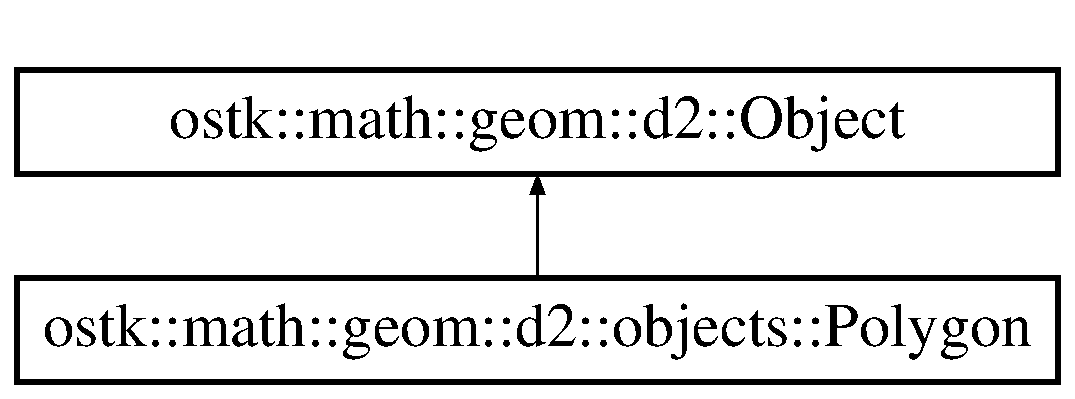
\includegraphics[height=2.000000cm]{classostk_1_1math_1_1geom_1_1d2_1_1objects_1_1_polygon}
\end{center}
\end{figure}
\doxysubsection*{Public Types}
\begin{DoxyCompactItemize}
\item 
typedef \mbox{\hyperlink{classostk_1_1math_1_1geom_1_1d2_1_1objects_1_1_point}{Point}} \mbox{\hyperlink{classostk_1_1math_1_1geom_1_1d2_1_1objects_1_1_polygon_a2fdf6254b42f087bd9cd0b8b0d7df91c}{Vertex}}
\item 
typedef \mbox{\hyperlink{classostk_1_1math_1_1geom_1_1d2_1_1objects_1_1_segment}{Segment}} \mbox{\hyperlink{classostk_1_1math_1_1geom_1_1d2_1_1objects_1_1_polygon_a85e5c92944c126a62464874b5a6ba490}{Edge}}
\item 
typedef \mbox{\hyperlink{classostk_1_1math_1_1geom_1_1d2_1_1objects_1_1_line_string}{Line\+String}} \mbox{\hyperlink{classostk_1_1math_1_1geom_1_1d2_1_1objects_1_1_polygon_a2cfc117e0bd669946a670640eae4ee4c}{Ring}}
\end{DoxyCompactItemize}
\doxysubsection*{Public Member Functions}
\begin{DoxyCompactItemize}
\item 
\mbox{\hyperlink{classostk_1_1math_1_1geom_1_1d2_1_1objects_1_1_polygon_adaf9ef564754ab10ed3dd0d5fa0d90ea}{Polygon}} (const Array$<$ \mbox{\hyperlink{classostk_1_1math_1_1geom_1_1d2_1_1objects_1_1_point}{Point}} $>$ \&an\+Outer\+Ring, const Array$<$ Array$<$ \mbox{\hyperlink{classostk_1_1math_1_1geom_1_1d2_1_1objects_1_1_point}{Point}} $>$$>$ \&an\+Inner\+Ring\+Array=Array$<$ Array$<$ \mbox{\hyperlink{classostk_1_1math_1_1geom_1_1d2_1_1objects_1_1_point}{Point}} $>$$>$\+::Empty())
\begin{DoxyCompactList}\small\item\em Constructor. \end{DoxyCompactList}\item 
\mbox{\hyperlink{classostk_1_1math_1_1geom_1_1d2_1_1objects_1_1_polygon_adebeb4b256cd7f772f62934c06431d27}{Polygon}} (const \mbox{\hyperlink{classostk_1_1math_1_1geom_1_1d2_1_1objects_1_1_polygon_a2cfc117e0bd669946a670640eae4ee4c}{Polygon\+::\+Ring}} \&an\+Outer\+Ring, const Array$<$ \mbox{\hyperlink{classostk_1_1math_1_1geom_1_1d2_1_1objects_1_1_polygon_a2cfc117e0bd669946a670640eae4ee4c}{Polygon\+::\+Ring}} $>$ \&an\+Inner\+Ring\+Array=Array$<$ \mbox{\hyperlink{classostk_1_1math_1_1geom_1_1d2_1_1objects_1_1_polygon_a2cfc117e0bd669946a670640eae4ee4c}{Polygon\+::\+Ring}} $>$\+::Empty())
\begin{DoxyCompactList}\small\item\em Constructor. \end{DoxyCompactList}\item 
\mbox{\hyperlink{classostk_1_1math_1_1geom_1_1d2_1_1objects_1_1_polygon_a191a97760bb334ede4b4181350d7b526}{Polygon}} (const \mbox{\hyperlink{classostk_1_1math_1_1geom_1_1d2_1_1objects_1_1_polygon}{Polygon}} \&a\+Polygon)
\begin{DoxyCompactList}\small\item\em Copy constructor. \end{DoxyCompactList}\item 
virtual \mbox{\hyperlink{classostk_1_1math_1_1geom_1_1d2_1_1objects_1_1_polygon_a26cd1c315770832bcb10c7c78f473ac1}{$\sim$\+Polygon}} () override
\begin{DoxyCompactList}\small\item\em Destructor (virtual) \end{DoxyCompactList}\item 
\mbox{\hyperlink{classostk_1_1math_1_1geom_1_1d2_1_1objects_1_1_polygon}{Polygon}} \& \mbox{\hyperlink{classostk_1_1math_1_1geom_1_1d2_1_1objects_1_1_polygon_aad1bdf4404a88c3da5c93e12e0cbb241}{operator=}} (const \mbox{\hyperlink{classostk_1_1math_1_1geom_1_1d2_1_1objects_1_1_polygon}{Polygon}} \&a\+Polygon)
\begin{DoxyCompactList}\small\item\em Copy assignment operator. \end{DoxyCompactList}\item 
virtual \mbox{\hyperlink{classostk_1_1math_1_1geom_1_1d2_1_1objects_1_1_polygon}{Polygon}} $\ast$ \mbox{\hyperlink{classostk_1_1math_1_1geom_1_1d2_1_1objects_1_1_polygon_a55e4524d1f58bf8379580e63f49f0b48}{clone}} () const override
\begin{DoxyCompactList}\small\item\em Clone polygon. \end{DoxyCompactList}\item 
bool \mbox{\hyperlink{classostk_1_1math_1_1geom_1_1d2_1_1objects_1_1_polygon_a6fa3a2d3811523250bbb916e5d0ff8b9}{operator==}} (const \mbox{\hyperlink{classostk_1_1math_1_1geom_1_1d2_1_1objects_1_1_polygon}{Polygon}} \&a\+Polygon) const
\begin{DoxyCompactList}\small\item\em Equal to operator. \end{DoxyCompactList}\item 
bool \mbox{\hyperlink{classostk_1_1math_1_1geom_1_1d2_1_1objects_1_1_polygon_a2a592e75608feeafd324105c65c67640}{operator!=}} (const \mbox{\hyperlink{classostk_1_1math_1_1geom_1_1d2_1_1objects_1_1_polygon}{Polygon}} \&a\+Polygon) const
\begin{DoxyCompactList}\small\item\em Not equal to operator. \end{DoxyCompactList}\item 
virtual bool \mbox{\hyperlink{classostk_1_1math_1_1geom_1_1d2_1_1objects_1_1_polygon_a81f92393dad2c6421fd4fe3834f60fa2}{is\+Defined}} () const override
\begin{DoxyCompactList}\small\item\em Check if polygon is defined. \end{DoxyCompactList}\item 
bool \mbox{\hyperlink{classostk_1_1math_1_1geom_1_1d2_1_1objects_1_1_polygon_a70a128f7d670604478947243e8a96937}{is\+Near}} (const \mbox{\hyperlink{classostk_1_1math_1_1geom_1_1d2_1_1objects_1_1_polygon}{Polygon}} \&a\+Polygon, const Real \&a\+Tolerance) const
\begin{DoxyCompactList}\small\item\em Check if polygon is near another polygon. \end{DoxyCompactList}\item 
bool \mbox{\hyperlink{classostk_1_1math_1_1geom_1_1d2_1_1objects_1_1_polygon_ad0183cbb840fe9f1fb9dfde0cc3eae50}{intersects}} (const \mbox{\hyperlink{classostk_1_1math_1_1geom_1_1d2_1_1objects_1_1_polygon}{Polygon}} \&a\+Polygon) const
\begin{DoxyCompactList}\small\item\em Check if polygon intersects polygon. \end{DoxyCompactList}\item 
bool \mbox{\hyperlink{classostk_1_1math_1_1geom_1_1d2_1_1objects_1_1_polygon_aa9f49a046d832821a8b26064b3cf2158}{contains}} (const \mbox{\hyperlink{classostk_1_1math_1_1geom_1_1d2_1_1objects_1_1_point}{Point}} \&a\+Point) const
\begin{DoxyCompactList}\small\item\em Check if polygon contains point. \end{DoxyCompactList}\item 
bool \mbox{\hyperlink{classostk_1_1math_1_1geom_1_1d2_1_1objects_1_1_polygon_a6a95f14d1bcbc3d0231ed09f31d17045}{contains}} (const \mbox{\hyperlink{classostk_1_1math_1_1geom_1_1d2_1_1objects_1_1_point_set}{Point\+Set}} \&a\+Point\+Set) const
\begin{DoxyCompactList}\small\item\em Check if polygon contains point set. \end{DoxyCompactList}\item 
bool \mbox{\hyperlink{classostk_1_1math_1_1geom_1_1d2_1_1objects_1_1_polygon_a203d0490d40b2a221f46194765e0435d}{contains}} (const \mbox{\hyperlink{classostk_1_1math_1_1geom_1_1d2_1_1objects_1_1_line_string}{Line\+String}} \&a\+Line\+String) const
\begin{DoxyCompactList}\small\item\em Check if polygon contains line string. \end{DoxyCompactList}\item 
Size \mbox{\hyperlink{classostk_1_1math_1_1geom_1_1d2_1_1objects_1_1_polygon_a47930b6706bc8b54754e064f0d0ec29b}{get\+Inner\+Ring\+Count}} () const
\begin{DoxyCompactList}\small\item\em Get number of inner rings. \end{DoxyCompactList}\item 
Size \mbox{\hyperlink{classostk_1_1math_1_1geom_1_1d2_1_1objects_1_1_polygon_a585310d630d1e80f496a9525a308bb2b}{get\+Edge\+Count}} () const
\begin{DoxyCompactList}\small\item\em Get edge count. \end{DoxyCompactList}\item 
Size \mbox{\hyperlink{classostk_1_1math_1_1geom_1_1d2_1_1objects_1_1_polygon_ac53efcb8236507a884323d5db2dd5cdf}{get\+Vertex\+Count}} () const
\begin{DoxyCompactList}\small\item\em Get vertex count. \end{DoxyCompactList}\item 
\mbox{\hyperlink{classostk_1_1math_1_1geom_1_1d2_1_1objects_1_1_polygon_a2cfc117e0bd669946a670640eae4ee4c}{Polygon\+::\+Ring}} \mbox{\hyperlink{classostk_1_1math_1_1geom_1_1d2_1_1objects_1_1_polygon_a051e05d5e1a0e7e1a3e14fd7441ebbf0}{get\+Outer\+Ring}} () const
\begin{DoxyCompactList}\small\item\em Get outer ring. \end{DoxyCompactList}\item 
\mbox{\hyperlink{classostk_1_1math_1_1geom_1_1d2_1_1objects_1_1_polygon_a2cfc117e0bd669946a670640eae4ee4c}{Polygon\+::\+Ring}} \mbox{\hyperlink{classostk_1_1math_1_1geom_1_1d2_1_1objects_1_1_polygon_af1974ca25ea35ce4857dcac525f1180c}{get\+Inner\+Ring\+At}} (const Index \&an\+Inner\+Ring\+Index) const
\begin{DoxyCompactList}\small\item\em Get inner ring at index. \end{DoxyCompactList}\item 
\mbox{\hyperlink{classostk_1_1math_1_1geom_1_1d2_1_1objects_1_1_polygon_a85e5c92944c126a62464874b5a6ba490}{Polygon\+::\+Edge}} \mbox{\hyperlink{classostk_1_1math_1_1geom_1_1d2_1_1objects_1_1_polygon_a247cba455e33ab1a05c43de43c27ba48}{get\+Edge\+At}} (const Index an\+Edge\+Index) const
\begin{DoxyCompactList}\small\item\em Get edge at index. \end{DoxyCompactList}\item 
\mbox{\hyperlink{classostk_1_1math_1_1geom_1_1d2_1_1objects_1_1_polygon_a2fdf6254b42f087bd9cd0b8b0d7df91c}{Polygon\+::\+Vertex}} \mbox{\hyperlink{classostk_1_1math_1_1geom_1_1d2_1_1objects_1_1_polygon_af3eff08fe9f9c74c5d9aebe7fb5f888f}{get\+Vertex\+At}} (const Index a\+Vertex\+Index) const
\begin{DoxyCompactList}\small\item\em Get vertex at index. \end{DoxyCompactList}\item 
Array$<$ \mbox{\hyperlink{classostk_1_1math_1_1geom_1_1d2_1_1objects_1_1_polygon_a85e5c92944c126a62464874b5a6ba490}{Polygon\+::\+Edge}} $>$ \mbox{\hyperlink{classostk_1_1math_1_1geom_1_1d2_1_1objects_1_1_polygon_ac0c151b62ba0798eb4d86b2458e6d8b0}{get\+Edges}} () const
\begin{DoxyCompactList}\small\item\em Get polygon edges. \end{DoxyCompactList}\item 
Array$<$ \mbox{\hyperlink{classostk_1_1math_1_1geom_1_1d2_1_1objects_1_1_polygon_a2fdf6254b42f087bd9cd0b8b0d7df91c}{Polygon\+::\+Vertex}} $>$ \mbox{\hyperlink{classostk_1_1math_1_1geom_1_1d2_1_1objects_1_1_polygon_a04a97204d397a1c7a919ebf4d73fb537}{get\+Vertices}} () const
\begin{DoxyCompactList}\small\item\em Get polygon vertices. \end{DoxyCompactList}\item 
\mbox{\hyperlink{classostk_1_1math_1_1geom_1_1d2_1_1objects_1_1_polygon}{Polygon}} \mbox{\hyperlink{classostk_1_1math_1_1geom_1_1d2_1_1objects_1_1_polygon_a82a1c0d6a76ee136829e0668bdd5c4a6}{get\+Convex\+Hull}} () const
\begin{DoxyCompactList}\small\item\em Get polygon convex hull. \end{DoxyCompactList}\item 
\mbox{\hyperlink{classostk_1_1math_1_1geom_1_1d2_1_1_intersection}{Intersection}} \mbox{\hyperlink{classostk_1_1math_1_1geom_1_1d2_1_1objects_1_1_polygon_a3be4f9a3cca08678f6050cdb8ae31618}{intersection\+With}} (const \mbox{\hyperlink{classostk_1_1math_1_1geom_1_1d2_1_1objects_1_1_polygon}{Polygon}} \&a\+Polygon) const
\begin{DoxyCompactList}\small\item\em Compute intersection of polygon with polygon. \end{DoxyCompactList}\item 
\mbox{\hyperlink{classostk_1_1math_1_1geom_1_1d2_1_1_intersection}{Intersection}} \mbox{\hyperlink{classostk_1_1math_1_1geom_1_1d2_1_1objects_1_1_polygon_aaea6f04037e95bd70e4d6f0524f129e9}{difference\+With}} (const \mbox{\hyperlink{classostk_1_1math_1_1geom_1_1d2_1_1objects_1_1_polygon}{Polygon}} \&a\+Polygon) const
\begin{DoxyCompactList}\small\item\em Compute difference of polygon with polygon. \end{DoxyCompactList}\item 
\mbox{\hyperlink{classostk_1_1math_1_1geom_1_1d2_1_1objects_1_1_multi_polygon}{Multi\+Polygon}} \mbox{\hyperlink{classostk_1_1math_1_1geom_1_1d2_1_1objects_1_1_polygon_ad01feda42e80b74752d3529bc122981b}{union\+With}} (const \mbox{\hyperlink{classostk_1_1math_1_1geom_1_1d2_1_1objects_1_1_polygon}{Polygon}} \&a\+Polygon) const
\begin{DoxyCompactList}\small\item\em Compute union of polygon with polygon. \end{DoxyCompactList}\item 
virtual String \mbox{\hyperlink{classostk_1_1math_1_1geom_1_1d2_1_1objects_1_1_polygon_a6e672ccf5f1101de80e636f097f0a0f7}{to\+String}} (const \mbox{\hyperlink{classostk_1_1math_1_1geom_1_1d2_1_1_object_aa76f9e30caebf4005bafbdff447f66cf}{Object\+::\+Format}} \&a\+Format=\mbox{\hyperlink{classostk_1_1math_1_1geom_1_1d2_1_1_object_aa76f9e30caebf4005bafbdff447f66cfaeb6d8ae6f20283755b339c0dc273988b}{Object\+::\+Format\+::\+Standard}}, const Integer \&a\+Precision=Integer\+::\+Undefined()) const override
\begin{DoxyCompactList}\small\item\em Get string representation. \end{DoxyCompactList}\item 
virtual void \mbox{\hyperlink{classostk_1_1math_1_1geom_1_1d2_1_1objects_1_1_polygon_adbf6ed9930a6dd2f3eab1c5c1b256ded}{print}} (std\+::ostream \&an\+Output\+Stream, bool display\+Decorators=true) const override
\begin{DoxyCompactList}\small\item\em Print polygon. \end{DoxyCompactList}\item 
virtual void \mbox{\hyperlink{classostk_1_1math_1_1geom_1_1d2_1_1objects_1_1_polygon_a00d04368f01daa0b234b403321453bbf}{apply\+Transformation}} (const \mbox{\hyperlink{classostk_1_1math_1_1geom_1_1d2_1_1_transformation}{Transformation}} \&a\+Transformation) override
\begin{DoxyCompactList}\small\item\em Apply transformation to polygon. \end{DoxyCompactList}\end{DoxyCompactItemize}
\doxysubsection*{Static Public Member Functions}
\begin{DoxyCompactItemize}
\item 
static \mbox{\hyperlink{classostk_1_1math_1_1geom_1_1d2_1_1objects_1_1_polygon}{Polygon}} \mbox{\hyperlink{classostk_1_1math_1_1geom_1_1d2_1_1objects_1_1_polygon_af260e109c9315fd31f7f24f3154dcbf2}{Undefined}} ()
\begin{DoxyCompactList}\small\item\em Constructs an undefined polygon. \end{DoxyCompactList}\end{DoxyCompactItemize}


\doxysubsection{Detailed Description}
\mbox{\hyperlink{classostk_1_1math_1_1geom_1_1d2_1_1objects_1_1_polygon}{Polygon}}. 

\begin{DoxyVerb}                        A plane figure that is bounded by a finite chain of straight line segments closing in a loop
                        to form a closed polygonal chain or circuit.
                        These segments are called its edges, and the points where two edges meet are the polygon's vertices.
\end{DoxyVerb}


\href{https://en.wikipedia.org/wiki/Polygon}{\texttt{ https\+://en.\+wikipedia.\+org/wiki/\+Polygon}} 

\doxysubsection{Member Typedef Documentation}
\mbox{\Hypertarget{classostk_1_1math_1_1geom_1_1d2_1_1objects_1_1_polygon_a85e5c92944c126a62464874b5a6ba490}\label{classostk_1_1math_1_1geom_1_1d2_1_1objects_1_1_polygon_a85e5c92944c126a62464874b5a6ba490}} 
\index{ostk::math::geom::d2::objects::Polygon@{ostk::math::geom::d2::objects::Polygon}!Edge@{Edge}}
\index{Edge@{Edge}!ostk::math::geom::d2::objects::Polygon@{ostk::math::geom::d2::objects::Polygon}}
\doxysubsubsection{\texorpdfstring{Edge}{Edge}}
{\footnotesize\ttfamily typedef \mbox{\hyperlink{classostk_1_1math_1_1geom_1_1d2_1_1objects_1_1_segment}{Segment}} \mbox{\hyperlink{classostk_1_1math_1_1geom_1_1d2_1_1objects_1_1_polygon_a85e5c92944c126a62464874b5a6ba490}{ostk\+::math\+::geom\+::d2\+::objects\+::\+Polygon\+::\+Edge}}}

\mbox{\Hypertarget{classostk_1_1math_1_1geom_1_1d2_1_1objects_1_1_polygon_a2cfc117e0bd669946a670640eae4ee4c}\label{classostk_1_1math_1_1geom_1_1d2_1_1objects_1_1_polygon_a2cfc117e0bd669946a670640eae4ee4c}} 
\index{ostk::math::geom::d2::objects::Polygon@{ostk::math::geom::d2::objects::Polygon}!Ring@{Ring}}
\index{Ring@{Ring}!ostk::math::geom::d2::objects::Polygon@{ostk::math::geom::d2::objects::Polygon}}
\doxysubsubsection{\texorpdfstring{Ring}{Ring}}
{\footnotesize\ttfamily typedef \mbox{\hyperlink{classostk_1_1math_1_1geom_1_1d2_1_1objects_1_1_line_string}{Line\+String}} \mbox{\hyperlink{classostk_1_1math_1_1geom_1_1d2_1_1objects_1_1_polygon_a2cfc117e0bd669946a670640eae4ee4c}{ostk\+::math\+::geom\+::d2\+::objects\+::\+Polygon\+::\+Ring}}}

\mbox{\Hypertarget{classostk_1_1math_1_1geom_1_1d2_1_1objects_1_1_polygon_a2fdf6254b42f087bd9cd0b8b0d7df91c}\label{classostk_1_1math_1_1geom_1_1d2_1_1objects_1_1_polygon_a2fdf6254b42f087bd9cd0b8b0d7df91c}} 
\index{ostk::math::geom::d2::objects::Polygon@{ostk::math::geom::d2::objects::Polygon}!Vertex@{Vertex}}
\index{Vertex@{Vertex}!ostk::math::geom::d2::objects::Polygon@{ostk::math::geom::d2::objects::Polygon}}
\doxysubsubsection{\texorpdfstring{Vertex}{Vertex}}
{\footnotesize\ttfamily typedef \mbox{\hyperlink{classostk_1_1math_1_1geom_1_1d2_1_1objects_1_1_point}{Point}} \mbox{\hyperlink{classostk_1_1math_1_1geom_1_1d2_1_1objects_1_1_polygon_a2fdf6254b42f087bd9cd0b8b0d7df91c}{ostk\+::math\+::geom\+::d2\+::objects\+::\+Polygon\+::\+Vertex}}}



\doxysubsection{Constructor \& Destructor Documentation}
\mbox{\Hypertarget{classostk_1_1math_1_1geom_1_1d2_1_1objects_1_1_polygon_adaf9ef564754ab10ed3dd0d5fa0d90ea}\label{classostk_1_1math_1_1geom_1_1d2_1_1objects_1_1_polygon_adaf9ef564754ab10ed3dd0d5fa0d90ea}} 
\index{ostk::math::geom::d2::objects::Polygon@{ostk::math::geom::d2::objects::Polygon}!Polygon@{Polygon}}
\index{Polygon@{Polygon}!ostk::math::geom::d2::objects::Polygon@{ostk::math::geom::d2::objects::Polygon}}
\doxysubsubsection{\texorpdfstring{Polygon()}{Polygon()}\hspace{0.1cm}{\footnotesize\ttfamily [1/3]}}
{\footnotesize\ttfamily ostk\+::math\+::geom\+::d2\+::objects\+::\+Polygon\+::\+Polygon (\begin{DoxyParamCaption}\item[{const Array$<$ \mbox{\hyperlink{classostk_1_1math_1_1geom_1_1d2_1_1objects_1_1_point}{Point}} $>$ \&}]{an\+Outer\+Ring,  }\item[{const Array$<$ Array$<$ \mbox{\hyperlink{classostk_1_1math_1_1geom_1_1d2_1_1objects_1_1_point}{Point}} $>$$>$ \&}]{an\+Inner\+Ring\+Array = {\ttfamily Array$<$Array$<$\mbox{\hyperlink{classostk_1_1math_1_1geom_1_1d2_1_1objects_1_1_point}{Point}}$>$$>$\+:\+:Empty()} }\end{DoxyParamCaption})}



Constructor. 


\begin{DoxyParams}[1]{Parameters}
\mbox{\texttt{ in}}  & {\em an\+Outer\+Ring} & An outer ring \\
\hline
\mbox{\texttt{ in}}  & {\em an\+Inner\+Ring\+Array} & An array of inner rings \\
\hline
\end{DoxyParams}
\mbox{\Hypertarget{classostk_1_1math_1_1geom_1_1d2_1_1objects_1_1_polygon_adebeb4b256cd7f772f62934c06431d27}\label{classostk_1_1math_1_1geom_1_1d2_1_1objects_1_1_polygon_adebeb4b256cd7f772f62934c06431d27}} 
\index{ostk::math::geom::d2::objects::Polygon@{ostk::math::geom::d2::objects::Polygon}!Polygon@{Polygon}}
\index{Polygon@{Polygon}!ostk::math::geom::d2::objects::Polygon@{ostk::math::geom::d2::objects::Polygon}}
\doxysubsubsection{\texorpdfstring{Polygon()}{Polygon()}\hspace{0.1cm}{\footnotesize\ttfamily [2/3]}}
{\footnotesize\ttfamily ostk\+::math\+::geom\+::d2\+::objects\+::\+Polygon\+::\+Polygon (\begin{DoxyParamCaption}\item[{const \mbox{\hyperlink{classostk_1_1math_1_1geom_1_1d2_1_1objects_1_1_polygon_a2cfc117e0bd669946a670640eae4ee4c}{Polygon\+::\+Ring}} \&}]{an\+Outer\+Ring,  }\item[{const Array$<$ \mbox{\hyperlink{classostk_1_1math_1_1geom_1_1d2_1_1objects_1_1_polygon_a2cfc117e0bd669946a670640eae4ee4c}{Polygon\+::\+Ring}} $>$ \&}]{an\+Inner\+Ring\+Array = {\ttfamily Array$<$~\mbox{\hyperlink{classostk_1_1math_1_1geom_1_1d2_1_1objects_1_1_polygon_a2cfc117e0bd669946a670640eae4ee4c}{Polygon\+::\+Ring}}~$>$\+:\+:Empty()} }\end{DoxyParamCaption})}



Constructor. 


\begin{DoxyParams}[1]{Parameters}
\mbox{\texttt{ in}}  & {\em an\+Outer\+Ring} & An outer ring \\
\hline
\mbox{\texttt{ in}}  & {\em an\+Inner\+Ring\+Array} & An array of inner rings \\
\hline
\end{DoxyParams}
\mbox{\Hypertarget{classostk_1_1math_1_1geom_1_1d2_1_1objects_1_1_polygon_a191a97760bb334ede4b4181350d7b526}\label{classostk_1_1math_1_1geom_1_1d2_1_1objects_1_1_polygon_a191a97760bb334ede4b4181350d7b526}} 
\index{ostk::math::geom::d2::objects::Polygon@{ostk::math::geom::d2::objects::Polygon}!Polygon@{Polygon}}
\index{Polygon@{Polygon}!ostk::math::geom::d2::objects::Polygon@{ostk::math::geom::d2::objects::Polygon}}
\doxysubsubsection{\texorpdfstring{Polygon()}{Polygon()}\hspace{0.1cm}{\footnotesize\ttfamily [3/3]}}
{\footnotesize\ttfamily ostk\+::math\+::geom\+::d2\+::objects\+::\+Polygon\+::\+Polygon (\begin{DoxyParamCaption}\item[{const \mbox{\hyperlink{classostk_1_1math_1_1geom_1_1d2_1_1objects_1_1_polygon}{Polygon}} \&}]{a\+Polygon }\end{DoxyParamCaption})}



Copy constructor. 


\begin{DoxyParams}[1]{Parameters}
\mbox{\texttt{ in}}  & {\em a\+Polygon} & A polygon \\
\hline
\end{DoxyParams}
\mbox{\Hypertarget{classostk_1_1math_1_1geom_1_1d2_1_1objects_1_1_polygon_a26cd1c315770832bcb10c7c78f473ac1}\label{classostk_1_1math_1_1geom_1_1d2_1_1objects_1_1_polygon_a26cd1c315770832bcb10c7c78f473ac1}} 
\index{ostk::math::geom::d2::objects::Polygon@{ostk::math::geom::d2::objects::Polygon}!````~Polygon@{$\sim$Polygon}}
\index{````~Polygon@{$\sim$Polygon}!ostk::math::geom::d2::objects::Polygon@{ostk::math::geom::d2::objects::Polygon}}
\doxysubsubsection{\texorpdfstring{$\sim$Polygon()}{~Polygon()}}
{\footnotesize\ttfamily ostk\+::math\+::geom\+::d2\+::objects\+::\+Polygon\+::$\sim$\+Polygon (\begin{DoxyParamCaption}{ }\end{DoxyParamCaption})\hspace{0.3cm}{\ttfamily [override]}, {\ttfamily [virtual]}}



Destructor (virtual) 



\doxysubsection{Member Function Documentation}
\mbox{\Hypertarget{classostk_1_1math_1_1geom_1_1d2_1_1objects_1_1_polygon_a00d04368f01daa0b234b403321453bbf}\label{classostk_1_1math_1_1geom_1_1d2_1_1objects_1_1_polygon_a00d04368f01daa0b234b403321453bbf}} 
\index{ostk::math::geom::d2::objects::Polygon@{ostk::math::geom::d2::objects::Polygon}!applyTransformation@{applyTransformation}}
\index{applyTransformation@{applyTransformation}!ostk::math::geom::d2::objects::Polygon@{ostk::math::geom::d2::objects::Polygon}}
\doxysubsubsection{\texorpdfstring{applyTransformation()}{applyTransformation()}}
{\footnotesize\ttfamily void ostk\+::math\+::geom\+::d2\+::objects\+::\+Polygon\+::apply\+Transformation (\begin{DoxyParamCaption}\item[{const \mbox{\hyperlink{classostk_1_1math_1_1geom_1_1d2_1_1_transformation}{Transformation}} \&}]{a\+Transformation }\end{DoxyParamCaption})\hspace{0.3cm}{\ttfamily [override]}, {\ttfamily [virtual]}}



Apply transformation to polygon. 


\begin{DoxyParams}[1]{Parameters}
\mbox{\texttt{ in}}  & {\em a\+Transformation} & A transformation \\
\hline
\end{DoxyParams}


Implements \mbox{\hyperlink{classostk_1_1math_1_1geom_1_1d2_1_1_object_a959e50211d7a680f7f904bbb752d75c9}{ostk\+::math\+::geom\+::d2\+::\+Object}}.

\mbox{\Hypertarget{classostk_1_1math_1_1geom_1_1d2_1_1objects_1_1_polygon_a55e4524d1f58bf8379580e63f49f0b48}\label{classostk_1_1math_1_1geom_1_1d2_1_1objects_1_1_polygon_a55e4524d1f58bf8379580e63f49f0b48}} 
\index{ostk::math::geom::d2::objects::Polygon@{ostk::math::geom::d2::objects::Polygon}!clone@{clone}}
\index{clone@{clone}!ostk::math::geom::d2::objects::Polygon@{ostk::math::geom::d2::objects::Polygon}}
\doxysubsubsection{\texorpdfstring{clone()}{clone()}}
{\footnotesize\ttfamily \mbox{\hyperlink{classostk_1_1math_1_1geom_1_1d2_1_1objects_1_1_polygon}{Polygon}} $\ast$ ostk\+::math\+::geom\+::d2\+::objects\+::\+Polygon\+::clone (\begin{DoxyParamCaption}{ }\end{DoxyParamCaption}) const\hspace{0.3cm}{\ttfamily [override]}, {\ttfamily [virtual]}}



Clone polygon. 

\begin{DoxyReturn}{Returns}
Pointer to cloned polygon 
\end{DoxyReturn}


Implements \mbox{\hyperlink{classostk_1_1math_1_1geom_1_1d2_1_1_object_a98dedc6792aef35308966ca768eb3e14}{ostk\+::math\+::geom\+::d2\+::\+Object}}.

\mbox{\Hypertarget{classostk_1_1math_1_1geom_1_1d2_1_1objects_1_1_polygon_a203d0490d40b2a221f46194765e0435d}\label{classostk_1_1math_1_1geom_1_1d2_1_1objects_1_1_polygon_a203d0490d40b2a221f46194765e0435d}} 
\index{ostk::math::geom::d2::objects::Polygon@{ostk::math::geom::d2::objects::Polygon}!contains@{contains}}
\index{contains@{contains}!ostk::math::geom::d2::objects::Polygon@{ostk::math::geom::d2::objects::Polygon}}
\doxysubsubsection{\texorpdfstring{contains()}{contains()}\hspace{0.1cm}{\footnotesize\ttfamily [1/3]}}
{\footnotesize\ttfamily bool ostk\+::math\+::geom\+::d2\+::objects\+::\+Polygon\+::contains (\begin{DoxyParamCaption}\item[{const \mbox{\hyperlink{classostk_1_1math_1_1geom_1_1d2_1_1objects_1_1_line_string}{Line\+String}} \&}]{a\+Line\+String }\end{DoxyParamCaption}) const}



Check if polygon contains line string. 


\begin{DoxyCode}{0}
\DoxyCodeLine{\mbox{\hyperlink{classostk_1_1math_1_1geom_1_1d2_1_1objects_1_1_polygon_adaf9ef564754ab10ed3dd0d5fa0d90ea}{Polygon}} polygon = ... ;}
\DoxyCodeLine{LineString lineString = ... ;}
\DoxyCodeLine{polygon.contains(lineString) ;}
\end{DoxyCode}



\begin{DoxyParams}[1]{Parameters}
\mbox{\texttt{ in}}  & {\em a\+Line\+Seting} & A line string \\
\hline
\end{DoxyParams}
\begin{DoxyReturn}{Returns}
True if polygon contains line string 
\end{DoxyReturn}
\mbox{\Hypertarget{classostk_1_1math_1_1geom_1_1d2_1_1objects_1_1_polygon_aa9f49a046d832821a8b26064b3cf2158}\label{classostk_1_1math_1_1geom_1_1d2_1_1objects_1_1_polygon_aa9f49a046d832821a8b26064b3cf2158}} 
\index{ostk::math::geom::d2::objects::Polygon@{ostk::math::geom::d2::objects::Polygon}!contains@{contains}}
\index{contains@{contains}!ostk::math::geom::d2::objects::Polygon@{ostk::math::geom::d2::objects::Polygon}}
\doxysubsubsection{\texorpdfstring{contains()}{contains()}\hspace{0.1cm}{\footnotesize\ttfamily [2/3]}}
{\footnotesize\ttfamily bool ostk\+::math\+::geom\+::d2\+::objects\+::\+Polygon\+::contains (\begin{DoxyParamCaption}\item[{const \mbox{\hyperlink{classostk_1_1math_1_1geom_1_1d2_1_1objects_1_1_point}{Point}} \&}]{a\+Point }\end{DoxyParamCaption}) const}



Check if polygon contains point. 


\begin{DoxyCode}{0}
\DoxyCodeLine{\mbox{\hyperlink{classostk_1_1math_1_1geom_1_1d2_1_1objects_1_1_polygon_adaf9ef564754ab10ed3dd0d5fa0d90ea}{Polygon}} polygon = ... ;}
\DoxyCodeLine{Point point = ... ;}
\DoxyCodeLine{polygon.contains(point) ;}
\end{DoxyCode}



\begin{DoxyParams}[1]{Parameters}
\mbox{\texttt{ in}}  & {\em a\+Point} & A point \\
\hline
\end{DoxyParams}
\begin{DoxyReturn}{Returns}
True if polygon contains point 
\end{DoxyReturn}
\mbox{\Hypertarget{classostk_1_1math_1_1geom_1_1d2_1_1objects_1_1_polygon_a6a95f14d1bcbc3d0231ed09f31d17045}\label{classostk_1_1math_1_1geom_1_1d2_1_1objects_1_1_polygon_a6a95f14d1bcbc3d0231ed09f31d17045}} 
\index{ostk::math::geom::d2::objects::Polygon@{ostk::math::geom::d2::objects::Polygon}!contains@{contains}}
\index{contains@{contains}!ostk::math::geom::d2::objects::Polygon@{ostk::math::geom::d2::objects::Polygon}}
\doxysubsubsection{\texorpdfstring{contains()}{contains()}\hspace{0.1cm}{\footnotesize\ttfamily [3/3]}}
{\footnotesize\ttfamily bool ostk\+::math\+::geom\+::d2\+::objects\+::\+Polygon\+::contains (\begin{DoxyParamCaption}\item[{const \mbox{\hyperlink{classostk_1_1math_1_1geom_1_1d2_1_1objects_1_1_point_set}{Point\+Set}} \&}]{a\+Point\+Set }\end{DoxyParamCaption}) const}



Check if polygon contains point set. 


\begin{DoxyCode}{0}
\DoxyCodeLine{\mbox{\hyperlink{classostk_1_1math_1_1geom_1_1d2_1_1objects_1_1_polygon_adaf9ef564754ab10ed3dd0d5fa0d90ea}{Polygon}} polygon = ... ;}
\DoxyCodeLine{PointSet pointSet = ... ;}
\DoxyCodeLine{polygon.contains(pointSet) ;}
\end{DoxyCode}



\begin{DoxyParams}[1]{Parameters}
\mbox{\texttt{ in}}  & {\em a\+Point\+Set} & A point set \\
\hline
\end{DoxyParams}
\begin{DoxyReturn}{Returns}
True if polygon contains point set 
\end{DoxyReturn}
\mbox{\Hypertarget{classostk_1_1math_1_1geom_1_1d2_1_1objects_1_1_polygon_aaea6f04037e95bd70e4d6f0524f129e9}\label{classostk_1_1math_1_1geom_1_1d2_1_1objects_1_1_polygon_aaea6f04037e95bd70e4d6f0524f129e9}} 
\index{ostk::math::geom::d2::objects::Polygon@{ostk::math::geom::d2::objects::Polygon}!differenceWith@{differenceWith}}
\index{differenceWith@{differenceWith}!ostk::math::geom::d2::objects::Polygon@{ostk::math::geom::d2::objects::Polygon}}
\doxysubsubsection{\texorpdfstring{differenceWith()}{differenceWith()}}
{\footnotesize\ttfamily \mbox{\hyperlink{classostk_1_1math_1_1geom_1_1d2_1_1_intersection}{Intersection}} ostk\+::math\+::geom\+::d2\+::objects\+::\+Polygon\+::difference\+With (\begin{DoxyParamCaption}\item[{const \mbox{\hyperlink{classostk_1_1math_1_1geom_1_1d2_1_1objects_1_1_polygon}{Polygon}} \&}]{a\+Polygon }\end{DoxyParamCaption}) const}



Compute difference of polygon with polygon. 


\begin{DoxyParams}[1]{Parameters}
\mbox{\texttt{ in}}  & {\em a\+Polygon} & A polygon \\
\hline
\end{DoxyParams}
\begin{DoxyReturn}{Returns}
Difference (leveraging \mbox{\hyperlink{classostk_1_1math_1_1geom_1_1d2_1_1_intersection}{Intersection}} class) of polygon with polygon 
\end{DoxyReturn}
\mbox{\Hypertarget{classostk_1_1math_1_1geom_1_1d2_1_1objects_1_1_polygon_a82a1c0d6a76ee136829e0668bdd5c4a6}\label{classostk_1_1math_1_1geom_1_1d2_1_1objects_1_1_polygon_a82a1c0d6a76ee136829e0668bdd5c4a6}} 
\index{ostk::math::geom::d2::objects::Polygon@{ostk::math::geom::d2::objects::Polygon}!getConvexHull@{getConvexHull}}
\index{getConvexHull@{getConvexHull}!ostk::math::geom::d2::objects::Polygon@{ostk::math::geom::d2::objects::Polygon}}
\doxysubsubsection{\texorpdfstring{getConvexHull()}{getConvexHull()}}
{\footnotesize\ttfamily \mbox{\hyperlink{classostk_1_1math_1_1geom_1_1d2_1_1objects_1_1_polygon}{Polygon}} ostk\+::math\+::geom\+::d2\+::objects\+::\+Polygon\+::get\+Convex\+Hull (\begin{DoxyParamCaption}{ }\end{DoxyParamCaption}) const}



Get polygon convex hull. 

\begin{DoxyVerb}                https://en.wikipedia.org/wiki/Convex_hull
\end{DoxyVerb}


\begin{DoxyReturn}{Returns}
\mbox{\hyperlink{classostk_1_1math_1_1geom_1_1d2_1_1objects_1_1_polygon}{Polygon}} convex hull 
\end{DoxyReturn}
\mbox{\Hypertarget{classostk_1_1math_1_1geom_1_1d2_1_1objects_1_1_polygon_a247cba455e33ab1a05c43de43c27ba48}\label{classostk_1_1math_1_1geom_1_1d2_1_1objects_1_1_polygon_a247cba455e33ab1a05c43de43c27ba48}} 
\index{ostk::math::geom::d2::objects::Polygon@{ostk::math::geom::d2::objects::Polygon}!getEdgeAt@{getEdgeAt}}
\index{getEdgeAt@{getEdgeAt}!ostk::math::geom::d2::objects::Polygon@{ostk::math::geom::d2::objects::Polygon}}
\doxysubsubsection{\texorpdfstring{getEdgeAt()}{getEdgeAt()}}
{\footnotesize\ttfamily \mbox{\hyperlink{classostk_1_1math_1_1geom_1_1d2_1_1objects_1_1_polygon_a85e5c92944c126a62464874b5a6ba490}{Polygon\+::\+Edge}} ostk\+::math\+::geom\+::d2\+::objects\+::\+Polygon\+::get\+Edge\+At (\begin{DoxyParamCaption}\item[{const Index}]{an\+Edge\+Index }\end{DoxyParamCaption}) const}



Get edge at index. 


\begin{DoxyParams}[1]{Parameters}
\mbox{\texttt{ in}}  & {\em an\+Edge\+Index} & An edge index \\
\hline
\end{DoxyParams}
\begin{DoxyReturn}{Returns}
Edge (segment) 
\end{DoxyReturn}
\mbox{\Hypertarget{classostk_1_1math_1_1geom_1_1d2_1_1objects_1_1_polygon_a585310d630d1e80f496a9525a308bb2b}\label{classostk_1_1math_1_1geom_1_1d2_1_1objects_1_1_polygon_a585310d630d1e80f496a9525a308bb2b}} 
\index{ostk::math::geom::d2::objects::Polygon@{ostk::math::geom::d2::objects::Polygon}!getEdgeCount@{getEdgeCount}}
\index{getEdgeCount@{getEdgeCount}!ostk::math::geom::d2::objects::Polygon@{ostk::math::geom::d2::objects::Polygon}}
\doxysubsubsection{\texorpdfstring{getEdgeCount()}{getEdgeCount()}}
{\footnotesize\ttfamily Size ostk\+::math\+::geom\+::d2\+::objects\+::\+Polygon\+::get\+Edge\+Count (\begin{DoxyParamCaption}{ }\end{DoxyParamCaption}) const}



Get edge count. 

\begin{DoxyReturn}{Returns}
Edge count 
\end{DoxyReturn}
\mbox{\Hypertarget{classostk_1_1math_1_1geom_1_1d2_1_1objects_1_1_polygon_ac0c151b62ba0798eb4d86b2458e6d8b0}\label{classostk_1_1math_1_1geom_1_1d2_1_1objects_1_1_polygon_ac0c151b62ba0798eb4d86b2458e6d8b0}} 
\index{ostk::math::geom::d2::objects::Polygon@{ostk::math::geom::d2::objects::Polygon}!getEdges@{getEdges}}
\index{getEdges@{getEdges}!ostk::math::geom::d2::objects::Polygon@{ostk::math::geom::d2::objects::Polygon}}
\doxysubsubsection{\texorpdfstring{getEdges()}{getEdges()}}
{\footnotesize\ttfamily Array$<$ \mbox{\hyperlink{classostk_1_1math_1_1geom_1_1d2_1_1objects_1_1_polygon_a85e5c92944c126a62464874b5a6ba490}{Polygon\+::\+Edge}} $>$ ostk\+::math\+::geom\+::d2\+::objects\+::\+Polygon\+::get\+Edges (\begin{DoxyParamCaption}{ }\end{DoxyParamCaption}) const}



Get polygon edges. 

\begin{DoxyReturn}{Returns}
\mbox{\hyperlink{classostk_1_1math_1_1geom_1_1d2_1_1objects_1_1_polygon}{Polygon}} edges 
\end{DoxyReturn}
\mbox{\Hypertarget{classostk_1_1math_1_1geom_1_1d2_1_1objects_1_1_polygon_af1974ca25ea35ce4857dcac525f1180c}\label{classostk_1_1math_1_1geom_1_1d2_1_1objects_1_1_polygon_af1974ca25ea35ce4857dcac525f1180c}} 
\index{ostk::math::geom::d2::objects::Polygon@{ostk::math::geom::d2::objects::Polygon}!getInnerRingAt@{getInnerRingAt}}
\index{getInnerRingAt@{getInnerRingAt}!ostk::math::geom::d2::objects::Polygon@{ostk::math::geom::d2::objects::Polygon}}
\doxysubsubsection{\texorpdfstring{getInnerRingAt()}{getInnerRingAt()}}
{\footnotesize\ttfamily \mbox{\hyperlink{classostk_1_1math_1_1geom_1_1d2_1_1objects_1_1_polygon_a2cfc117e0bd669946a670640eae4ee4c}{Polygon\+::\+Ring}} ostk\+::math\+::geom\+::d2\+::objects\+::\+Polygon\+::get\+Inner\+Ring\+At (\begin{DoxyParamCaption}\item[{const Index \&}]{an\+Inner\+Ring\+Index }\end{DoxyParamCaption}) const}



Get inner ring at index. 

\begin{DoxyReturn}{Returns}
Inner ring at index 
\end{DoxyReturn}
\mbox{\Hypertarget{classostk_1_1math_1_1geom_1_1d2_1_1objects_1_1_polygon_a47930b6706bc8b54754e064f0d0ec29b}\label{classostk_1_1math_1_1geom_1_1d2_1_1objects_1_1_polygon_a47930b6706bc8b54754e064f0d0ec29b}} 
\index{ostk::math::geom::d2::objects::Polygon@{ostk::math::geom::d2::objects::Polygon}!getInnerRingCount@{getInnerRingCount}}
\index{getInnerRingCount@{getInnerRingCount}!ostk::math::geom::d2::objects::Polygon@{ostk::math::geom::d2::objects::Polygon}}
\doxysubsubsection{\texorpdfstring{getInnerRingCount()}{getInnerRingCount()}}
{\footnotesize\ttfamily Size ostk\+::math\+::geom\+::d2\+::objects\+::\+Polygon\+::get\+Inner\+Ring\+Count (\begin{DoxyParamCaption}{ }\end{DoxyParamCaption}) const}



Get number of inner rings. 

\begin{DoxyReturn}{Returns}
Number of inner rings 
\end{DoxyReturn}
\mbox{\Hypertarget{classostk_1_1math_1_1geom_1_1d2_1_1objects_1_1_polygon_a051e05d5e1a0e7e1a3e14fd7441ebbf0}\label{classostk_1_1math_1_1geom_1_1d2_1_1objects_1_1_polygon_a051e05d5e1a0e7e1a3e14fd7441ebbf0}} 
\index{ostk::math::geom::d2::objects::Polygon@{ostk::math::geom::d2::objects::Polygon}!getOuterRing@{getOuterRing}}
\index{getOuterRing@{getOuterRing}!ostk::math::geom::d2::objects::Polygon@{ostk::math::geom::d2::objects::Polygon}}
\doxysubsubsection{\texorpdfstring{getOuterRing()}{getOuterRing()}}
{\footnotesize\ttfamily \mbox{\hyperlink{classostk_1_1math_1_1geom_1_1d2_1_1objects_1_1_polygon_a2cfc117e0bd669946a670640eae4ee4c}{Polygon\+::\+Ring}} ostk\+::math\+::geom\+::d2\+::objects\+::\+Polygon\+::get\+Outer\+Ring (\begin{DoxyParamCaption}{ }\end{DoxyParamCaption}) const}



Get outer ring. 

\begin{DoxyReturn}{Returns}
Outer ring 
\end{DoxyReturn}
\mbox{\Hypertarget{classostk_1_1math_1_1geom_1_1d2_1_1objects_1_1_polygon_af3eff08fe9f9c74c5d9aebe7fb5f888f}\label{classostk_1_1math_1_1geom_1_1d2_1_1objects_1_1_polygon_af3eff08fe9f9c74c5d9aebe7fb5f888f}} 
\index{ostk::math::geom::d2::objects::Polygon@{ostk::math::geom::d2::objects::Polygon}!getVertexAt@{getVertexAt}}
\index{getVertexAt@{getVertexAt}!ostk::math::geom::d2::objects::Polygon@{ostk::math::geom::d2::objects::Polygon}}
\doxysubsubsection{\texorpdfstring{getVertexAt()}{getVertexAt()}}
{\footnotesize\ttfamily \mbox{\hyperlink{classostk_1_1math_1_1geom_1_1d2_1_1objects_1_1_polygon_a2fdf6254b42f087bd9cd0b8b0d7df91c}{Polygon\+::\+Vertex}} ostk\+::math\+::geom\+::d2\+::objects\+::\+Polygon\+::get\+Vertex\+At (\begin{DoxyParamCaption}\item[{const Index}]{a\+Vertex\+Index }\end{DoxyParamCaption}) const}



Get vertex at index. 


\begin{DoxyParams}[1]{Parameters}
\mbox{\texttt{ in}}  & {\em a\+Vertex\+Index} & A vertex index \\
\hline
\end{DoxyParams}
\begin{DoxyReturn}{Returns}
Vertex 
\end{DoxyReturn}
\mbox{\Hypertarget{classostk_1_1math_1_1geom_1_1d2_1_1objects_1_1_polygon_ac53efcb8236507a884323d5db2dd5cdf}\label{classostk_1_1math_1_1geom_1_1d2_1_1objects_1_1_polygon_ac53efcb8236507a884323d5db2dd5cdf}} 
\index{ostk::math::geom::d2::objects::Polygon@{ostk::math::geom::d2::objects::Polygon}!getVertexCount@{getVertexCount}}
\index{getVertexCount@{getVertexCount}!ostk::math::geom::d2::objects::Polygon@{ostk::math::geom::d2::objects::Polygon}}
\doxysubsubsection{\texorpdfstring{getVertexCount()}{getVertexCount()}}
{\footnotesize\ttfamily Size ostk\+::math\+::geom\+::d2\+::objects\+::\+Polygon\+::get\+Vertex\+Count (\begin{DoxyParamCaption}{ }\end{DoxyParamCaption}) const}



Get vertex count. 

\begin{DoxyReturn}{Returns}
Vertex count 
\end{DoxyReturn}
\mbox{\Hypertarget{classostk_1_1math_1_1geom_1_1d2_1_1objects_1_1_polygon_a04a97204d397a1c7a919ebf4d73fb537}\label{classostk_1_1math_1_1geom_1_1d2_1_1objects_1_1_polygon_a04a97204d397a1c7a919ebf4d73fb537}} 
\index{ostk::math::geom::d2::objects::Polygon@{ostk::math::geom::d2::objects::Polygon}!getVertices@{getVertices}}
\index{getVertices@{getVertices}!ostk::math::geom::d2::objects::Polygon@{ostk::math::geom::d2::objects::Polygon}}
\doxysubsubsection{\texorpdfstring{getVertices()}{getVertices()}}
{\footnotesize\ttfamily Array$<$ \mbox{\hyperlink{classostk_1_1math_1_1geom_1_1d2_1_1objects_1_1_polygon_a2fdf6254b42f087bd9cd0b8b0d7df91c}{Polygon\+::\+Vertex}} $>$ ostk\+::math\+::geom\+::d2\+::objects\+::\+Polygon\+::get\+Vertices (\begin{DoxyParamCaption}{ }\end{DoxyParamCaption}) const}



Get polygon vertices. 

\begin{DoxyReturn}{Returns}
\mbox{\hyperlink{classostk_1_1math_1_1geom_1_1d2_1_1objects_1_1_polygon}{Polygon}} vertices 
\end{DoxyReturn}
\mbox{\Hypertarget{classostk_1_1math_1_1geom_1_1d2_1_1objects_1_1_polygon_a3be4f9a3cca08678f6050cdb8ae31618}\label{classostk_1_1math_1_1geom_1_1d2_1_1objects_1_1_polygon_a3be4f9a3cca08678f6050cdb8ae31618}} 
\index{ostk::math::geom::d2::objects::Polygon@{ostk::math::geom::d2::objects::Polygon}!intersectionWith@{intersectionWith}}
\index{intersectionWith@{intersectionWith}!ostk::math::geom::d2::objects::Polygon@{ostk::math::geom::d2::objects::Polygon}}
\doxysubsubsection{\texorpdfstring{intersectionWith()}{intersectionWith()}}
{\footnotesize\ttfamily \mbox{\hyperlink{classostk_1_1math_1_1geom_1_1d2_1_1_intersection}{Intersection}} ostk\+::math\+::geom\+::d2\+::objects\+::\+Polygon\+::intersection\+With (\begin{DoxyParamCaption}\item[{const \mbox{\hyperlink{classostk_1_1math_1_1geom_1_1d2_1_1objects_1_1_polygon}{Polygon}} \&}]{a\+Polygon }\end{DoxyParamCaption}) const}



Compute intersection of polygon with polygon. 


\begin{DoxyParams}[1]{Parameters}
\mbox{\texttt{ in}}  & {\em a\+Polygon} & A polygon \\
\hline
\end{DoxyParams}
\begin{DoxyReturn}{Returns}
\mbox{\hyperlink{classostk_1_1math_1_1geom_1_1d2_1_1_intersection}{Intersection}} of polygon with polygon 
\end{DoxyReturn}
\mbox{\Hypertarget{classostk_1_1math_1_1geom_1_1d2_1_1objects_1_1_polygon_ad0183cbb840fe9f1fb9dfde0cc3eae50}\label{classostk_1_1math_1_1geom_1_1d2_1_1objects_1_1_polygon_ad0183cbb840fe9f1fb9dfde0cc3eae50}} 
\index{ostk::math::geom::d2::objects::Polygon@{ostk::math::geom::d2::objects::Polygon}!intersects@{intersects}}
\index{intersects@{intersects}!ostk::math::geom::d2::objects::Polygon@{ostk::math::geom::d2::objects::Polygon}}
\doxysubsubsection{\texorpdfstring{intersects()}{intersects()}}
{\footnotesize\ttfamily bool ostk\+::math\+::geom\+::d2\+::objects\+::\+Polygon\+::intersects (\begin{DoxyParamCaption}\item[{const \mbox{\hyperlink{classostk_1_1math_1_1geom_1_1d2_1_1objects_1_1_polygon}{Polygon}} \&}]{a\+Polygon }\end{DoxyParamCaption}) const}



Check if polygon intersects polygon. 


\begin{DoxyCode}{0}
\DoxyCodeLine{\mbox{\hyperlink{classostk_1_1math_1_1geom_1_1d2_1_1objects_1_1_polygon_adaf9ef564754ab10ed3dd0d5fa0d90ea}{Polygon}} polygon = ... ;}
\DoxyCodeLine{\mbox{\hyperlink{classostk_1_1math_1_1geom_1_1d2_1_1objects_1_1_polygon_adaf9ef564754ab10ed3dd0d5fa0d90ea}{Polygon}} anotherPolygon = ... ;}
\DoxyCodeLine{polygon.intersects(anotherPolygon) ;}
\end{DoxyCode}



\begin{DoxyParams}[1]{Parameters}
\mbox{\texttt{ in}}  & {\em a\+Polygon} & A polygon \\
\hline
\end{DoxyParams}
\begin{DoxyReturn}{Returns}
True if polygon intersects polygon 
\end{DoxyReturn}
\mbox{\Hypertarget{classostk_1_1math_1_1geom_1_1d2_1_1objects_1_1_polygon_a81f92393dad2c6421fd4fe3834f60fa2}\label{classostk_1_1math_1_1geom_1_1d2_1_1objects_1_1_polygon_a81f92393dad2c6421fd4fe3834f60fa2}} 
\index{ostk::math::geom::d2::objects::Polygon@{ostk::math::geom::d2::objects::Polygon}!isDefined@{isDefined}}
\index{isDefined@{isDefined}!ostk::math::geom::d2::objects::Polygon@{ostk::math::geom::d2::objects::Polygon}}
\doxysubsubsection{\texorpdfstring{isDefined()}{isDefined()}}
{\footnotesize\ttfamily bool ostk\+::math\+::geom\+::d2\+::objects\+::\+Polygon\+::is\+Defined (\begin{DoxyParamCaption}{ }\end{DoxyParamCaption}) const\hspace{0.3cm}{\ttfamily [override]}, {\ttfamily [virtual]}}



Check if polygon is defined. 

\begin{DoxyReturn}{Returns}
True if polygon is defined 
\end{DoxyReturn}


Implements \mbox{\hyperlink{classostk_1_1math_1_1geom_1_1d2_1_1_object_a456cc7121218d24c1322d0fe54230cc4}{ostk\+::math\+::geom\+::d2\+::\+Object}}.

\mbox{\Hypertarget{classostk_1_1math_1_1geom_1_1d2_1_1objects_1_1_polygon_a70a128f7d670604478947243e8a96937}\label{classostk_1_1math_1_1geom_1_1d2_1_1objects_1_1_polygon_a70a128f7d670604478947243e8a96937}} 
\index{ostk::math::geom::d2::objects::Polygon@{ostk::math::geom::d2::objects::Polygon}!isNear@{isNear}}
\index{isNear@{isNear}!ostk::math::geom::d2::objects::Polygon@{ostk::math::geom::d2::objects::Polygon}}
\doxysubsubsection{\texorpdfstring{isNear()}{isNear()}}
{\footnotesize\ttfamily bool ostk\+::math\+::geom\+::d2\+::objects\+::\+Polygon\+::is\+Near (\begin{DoxyParamCaption}\item[{const \mbox{\hyperlink{classostk_1_1math_1_1geom_1_1d2_1_1objects_1_1_polygon}{Polygon}} \&}]{a\+Polygon,  }\item[{const Real \&}]{a\+Tolerance }\end{DoxyParamCaption}) const}



Check if polygon is near another polygon. 


\begin{DoxyParams}[1]{Parameters}
\mbox{\texttt{ in}}  & {\em a\+Polygon} & A polygon \\
\hline
\mbox{\texttt{ in}}  & {\em a\+Tolerance} & A tolerance \\
\hline
\end{DoxyParams}
\begin{DoxyReturn}{Returns}
True if polygon is near another polygon 
\end{DoxyReturn}
\mbox{\Hypertarget{classostk_1_1math_1_1geom_1_1d2_1_1objects_1_1_polygon_a2a592e75608feeafd324105c65c67640}\label{classostk_1_1math_1_1geom_1_1d2_1_1objects_1_1_polygon_a2a592e75608feeafd324105c65c67640}} 
\index{ostk::math::geom::d2::objects::Polygon@{ostk::math::geom::d2::objects::Polygon}!operator"!=@{operator"!=}}
\index{operator"!=@{operator"!=}!ostk::math::geom::d2::objects::Polygon@{ostk::math::geom::d2::objects::Polygon}}
\doxysubsubsection{\texorpdfstring{operator"!=()}{operator!=()}}
{\footnotesize\ttfamily bool ostk\+::math\+::geom\+::d2\+::objects\+::\+Polygon\+::operator!= (\begin{DoxyParamCaption}\item[{const \mbox{\hyperlink{classostk_1_1math_1_1geom_1_1d2_1_1objects_1_1_polygon}{Polygon}} \&}]{a\+Polygon }\end{DoxyParamCaption}) const}



Not equal to operator. 


\begin{DoxyParams}[1]{Parameters}
\mbox{\texttt{ in}}  & {\em a\+Polygon} & A polygon \\
\hline
\end{DoxyParams}
\begin{DoxyReturn}{Returns}
True if polygons are not equal 
\end{DoxyReturn}
\mbox{\Hypertarget{classostk_1_1math_1_1geom_1_1d2_1_1objects_1_1_polygon_aad1bdf4404a88c3da5c93e12e0cbb241}\label{classostk_1_1math_1_1geom_1_1d2_1_1objects_1_1_polygon_aad1bdf4404a88c3da5c93e12e0cbb241}} 
\index{ostk::math::geom::d2::objects::Polygon@{ostk::math::geom::d2::objects::Polygon}!operator=@{operator=}}
\index{operator=@{operator=}!ostk::math::geom::d2::objects::Polygon@{ostk::math::geom::d2::objects::Polygon}}
\doxysubsubsection{\texorpdfstring{operator=()}{operator=()}}
{\footnotesize\ttfamily \mbox{\hyperlink{classostk_1_1math_1_1geom_1_1d2_1_1objects_1_1_polygon}{Polygon}} \& ostk\+::math\+::geom\+::d2\+::objects\+::\+Polygon\+::operator= (\begin{DoxyParamCaption}\item[{const \mbox{\hyperlink{classostk_1_1math_1_1geom_1_1d2_1_1objects_1_1_polygon}{Polygon}} \&}]{a\+Polygon }\end{DoxyParamCaption})}



Copy assignment operator. 


\begin{DoxyParams}[1]{Parameters}
\mbox{\texttt{ in}}  & {\em a\+Polygon} & A polygon \\
\hline
\end{DoxyParams}
\begin{DoxyReturn}{Returns}
Reference to polygon 
\end{DoxyReturn}
\mbox{\Hypertarget{classostk_1_1math_1_1geom_1_1d2_1_1objects_1_1_polygon_a6fa3a2d3811523250bbb916e5d0ff8b9}\label{classostk_1_1math_1_1geom_1_1d2_1_1objects_1_1_polygon_a6fa3a2d3811523250bbb916e5d0ff8b9}} 
\index{ostk::math::geom::d2::objects::Polygon@{ostk::math::geom::d2::objects::Polygon}!operator==@{operator==}}
\index{operator==@{operator==}!ostk::math::geom::d2::objects::Polygon@{ostk::math::geom::d2::objects::Polygon}}
\doxysubsubsection{\texorpdfstring{operator==()}{operator==()}}
{\footnotesize\ttfamily bool ostk\+::math\+::geom\+::d2\+::objects\+::\+Polygon\+::operator== (\begin{DoxyParamCaption}\item[{const \mbox{\hyperlink{classostk_1_1math_1_1geom_1_1d2_1_1objects_1_1_polygon}{Polygon}} \&}]{a\+Polygon }\end{DoxyParamCaption}) const}



Equal to operator. 


\begin{DoxyParams}[1]{Parameters}
\mbox{\texttt{ in}}  & {\em a\+Polygon} & A polygon \\
\hline
\end{DoxyParams}
\begin{DoxyReturn}{Returns}
True if polygons are equal 
\end{DoxyReturn}
\mbox{\Hypertarget{classostk_1_1math_1_1geom_1_1d2_1_1objects_1_1_polygon_adbf6ed9930a6dd2f3eab1c5c1b256ded}\label{classostk_1_1math_1_1geom_1_1d2_1_1objects_1_1_polygon_adbf6ed9930a6dd2f3eab1c5c1b256ded}} 
\index{ostk::math::geom::d2::objects::Polygon@{ostk::math::geom::d2::objects::Polygon}!print@{print}}
\index{print@{print}!ostk::math::geom::d2::objects::Polygon@{ostk::math::geom::d2::objects::Polygon}}
\doxysubsubsection{\texorpdfstring{print()}{print()}}
{\footnotesize\ttfamily void ostk\+::math\+::geom\+::d2\+::objects\+::\+Polygon\+::print (\begin{DoxyParamCaption}\item[{std\+::ostream \&}]{an\+Output\+Stream,  }\item[{bool}]{display\+Decorators = {\ttfamily true} }\end{DoxyParamCaption}) const\hspace{0.3cm}{\ttfamily [override]}, {\ttfamily [virtual]}}



Print polygon. 


\begin{DoxyParams}[1]{Parameters}
\mbox{\texttt{ in}}  & {\em an\+Output\+Stream} & An output stream \\
\hline
\mbox{\texttt{ in}}  & {\em (optional)} & display\+Decorators If true, display decorators \\
\hline
\end{DoxyParams}


Implements \mbox{\hyperlink{classostk_1_1math_1_1geom_1_1d2_1_1_object_ae05ad883ed5a560e38f0aae7a4adc1ea}{ostk\+::math\+::geom\+::d2\+::\+Object}}.

\mbox{\Hypertarget{classostk_1_1math_1_1geom_1_1d2_1_1objects_1_1_polygon_a6e672ccf5f1101de80e636f097f0a0f7}\label{classostk_1_1math_1_1geom_1_1d2_1_1objects_1_1_polygon_a6e672ccf5f1101de80e636f097f0a0f7}} 
\index{ostk::math::geom::d2::objects::Polygon@{ostk::math::geom::d2::objects::Polygon}!toString@{toString}}
\index{toString@{toString}!ostk::math::geom::d2::objects::Polygon@{ostk::math::geom::d2::objects::Polygon}}
\doxysubsubsection{\texorpdfstring{toString()}{toString()}}
{\footnotesize\ttfamily String ostk\+::math\+::geom\+::d2\+::objects\+::\+Polygon\+::to\+String (\begin{DoxyParamCaption}\item[{const \mbox{\hyperlink{classostk_1_1math_1_1geom_1_1d2_1_1_object_aa76f9e30caebf4005bafbdff447f66cf}{Object\+::\+Format}} \&}]{a\+Format = {\ttfamily \mbox{\hyperlink{classostk_1_1math_1_1geom_1_1d2_1_1_object_aa76f9e30caebf4005bafbdff447f66cfaeb6d8ae6f20283755b339c0dc273988b}{Object\+::\+Format\+::\+Standard}}},  }\item[{const Integer \&}]{a\+Precision = {\ttfamily Integer\+:\+:Undefined()} }\end{DoxyParamCaption}) const\hspace{0.3cm}{\ttfamily [override]}, {\ttfamily [virtual]}}



Get string representation. 


\begin{DoxyParams}[1]{Parameters}
\mbox{\texttt{ in}}  & {\em a\+Format} & A format \\
\hline
\end{DoxyParams}
\begin{DoxyReturn}{Returns}
String representation 
\end{DoxyReturn}


Implements \mbox{\hyperlink{classostk_1_1math_1_1geom_1_1d2_1_1_object_ada4c2187dd24ef02b91b6346191f677c}{ostk\+::math\+::geom\+::d2\+::\+Object}}.

\mbox{\Hypertarget{classostk_1_1math_1_1geom_1_1d2_1_1objects_1_1_polygon_af260e109c9315fd31f7f24f3154dcbf2}\label{classostk_1_1math_1_1geom_1_1d2_1_1objects_1_1_polygon_af260e109c9315fd31f7f24f3154dcbf2}} 
\index{ostk::math::geom::d2::objects::Polygon@{ostk::math::geom::d2::objects::Polygon}!Undefined@{Undefined}}
\index{Undefined@{Undefined}!ostk::math::geom::d2::objects::Polygon@{ostk::math::geom::d2::objects::Polygon}}
\doxysubsubsection{\texorpdfstring{Undefined()}{Undefined()}}
{\footnotesize\ttfamily \mbox{\hyperlink{classostk_1_1math_1_1geom_1_1d2_1_1objects_1_1_polygon}{Polygon}} ostk\+::math\+::geom\+::d2\+::objects\+::\+Polygon\+::\+Undefined (\begin{DoxyParamCaption}{ }\end{DoxyParamCaption})\hspace{0.3cm}{\ttfamily [static]}}



Constructs an undefined polygon. 


\begin{DoxyCode}{0}
\DoxyCodeLine{\mbox{\hyperlink{classostk_1_1math_1_1geom_1_1d2_1_1objects_1_1_polygon_adaf9ef564754ab10ed3dd0d5fa0d90ea}{Polygon}} polygon = \mbox{\hyperlink{classostk_1_1math_1_1geom_1_1d2_1_1objects_1_1_polygon_af260e109c9315fd31f7f24f3154dcbf2}{Polygon::Undefined}}() ; \textcolor{comment}{// Undefined}}
\end{DoxyCode}


\begin{DoxyReturn}{Returns}
Undefined polygon 
\end{DoxyReturn}
\mbox{\Hypertarget{classostk_1_1math_1_1geom_1_1d2_1_1objects_1_1_polygon_ad01feda42e80b74752d3529bc122981b}\label{classostk_1_1math_1_1geom_1_1d2_1_1objects_1_1_polygon_ad01feda42e80b74752d3529bc122981b}} 
\index{ostk::math::geom::d2::objects::Polygon@{ostk::math::geom::d2::objects::Polygon}!unionWith@{unionWith}}
\index{unionWith@{unionWith}!ostk::math::geom::d2::objects::Polygon@{ostk::math::geom::d2::objects::Polygon}}
\doxysubsubsection{\texorpdfstring{unionWith()}{unionWith()}}
{\footnotesize\ttfamily \mbox{\hyperlink{classostk_1_1math_1_1geom_1_1d2_1_1objects_1_1_multi_polygon}{Multi\+Polygon}} ostk\+::math\+::geom\+::d2\+::objects\+::\+Polygon\+::union\+With (\begin{DoxyParamCaption}\item[{const \mbox{\hyperlink{classostk_1_1math_1_1geom_1_1d2_1_1objects_1_1_polygon}{Polygon}} \&}]{a\+Polygon }\end{DoxyParamCaption}) const}



Compute union of polygon with polygon. 


\begin{DoxyParams}[1]{Parameters}
\mbox{\texttt{ in}}  & {\em a\+Polygon} & A polygon \\
\hline
\end{DoxyParams}
\begin{DoxyReturn}{Returns}
A multi-\/polygon 
\end{DoxyReturn}


The documentation for this class was generated from the following files\+:\begin{DoxyCompactItemize}
\item 
include/\+Open\+Space\+Toolkit/\+Mathematics/\+Geometry/2\+D/\+Objects/\mbox{\hyperlink{2_d_2_objects_2_polygon_8hpp}{Polygon.\+hpp}}\item 
src/\+Open\+Space\+Toolkit/\+Mathematics/\+Geometry/2\+D/\+Objects/\mbox{\hyperlink{2_d_2_objects_2_polygon_8cpp}{Polygon.\+cpp}}\end{DoxyCompactItemize}

\hypertarget{classostk_1_1math_1_1geom_1_1d3_1_1objects_1_1_polygon}{}\doxysection{ostk\+::math\+::geom\+::d3\+::objects\+::Polygon Class Reference}
\label{classostk_1_1math_1_1geom_1_1d3_1_1objects_1_1_polygon}\index{ostk::math::geom::d3::objects::Polygon@{ostk::math::geom::d3::objects::Polygon}}


\mbox{\hyperlink{classostk_1_1math_1_1geom_1_1d3_1_1objects_1_1_polygon}{Polygon}}.  




{\ttfamily \#include $<$Polygon.\+hpp$>$}

Inheritance diagram for ostk\+::math\+::geom\+::d3\+::objects\+::Polygon\+:\begin{figure}[H]
\begin{center}
\leavevmode
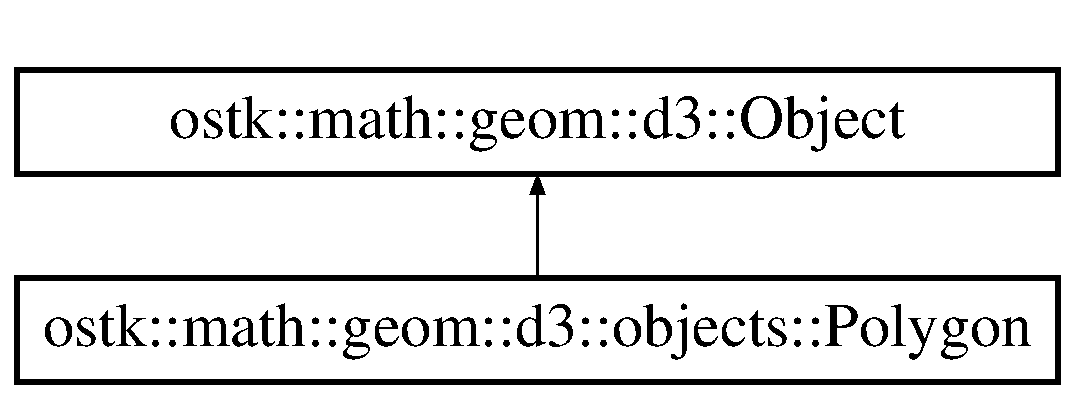
\includegraphics[height=2.000000cm]{classostk_1_1math_1_1geom_1_1d3_1_1objects_1_1_polygon}
\end{center}
\end{figure}
\doxysubsection*{Public Types}
\begin{DoxyCompactItemize}
\item 
typedef \mbox{\hyperlink{classostk_1_1math_1_1geom_1_1d3_1_1objects_1_1_point}{Point}} \mbox{\hyperlink{classostk_1_1math_1_1geom_1_1d3_1_1objects_1_1_polygon_a314eaf277355d59f5e6ab775702c47c2}{Vertex}}
\item 
typedef \mbox{\hyperlink{classostk_1_1math_1_1geom_1_1d3_1_1objects_1_1_segment}{Segment}} \mbox{\hyperlink{classostk_1_1math_1_1geom_1_1d3_1_1objects_1_1_polygon_a58c9a7e93e903b2226804116cce4f1ec}{Edge}}
\item 
typedef \mbox{\hyperlink{classostk_1_1math_1_1geom_1_1d3_1_1objects_1_1_line_string}{Line\+String}} \mbox{\hyperlink{classostk_1_1math_1_1geom_1_1d3_1_1objects_1_1_polygon_a5c06c7fb605535e012b1f362ed3a38c6}{Ring}}
\end{DoxyCompactItemize}
\doxysubsection*{Public Member Functions}
\begin{DoxyCompactItemize}
\item 
\mbox{\hyperlink{classostk_1_1math_1_1geom_1_1d3_1_1objects_1_1_polygon_a35918431f15eeac44436e0d39c949dd7}{Polygon}} (const \mbox{\hyperlink{namespaceostk_1_1math_1_1geom_1_1d3_1_1objects_ab51647b491a750a403dcaca4c2254905}{Polygon2d}} \&a\+Polygon, const \mbox{\hyperlink{classostk_1_1math_1_1geom_1_1d3_1_1objects_1_1_point}{Point}} \&an\+Origin, const Vector3d \&a\+X\+Axis, const Vector3d \&a\+Y\+Axis)
\begin{DoxyCompactList}\small\item\em Constructor. \end{DoxyCompactList}\item 
virtual \mbox{\hyperlink{classostk_1_1math_1_1geom_1_1d3_1_1objects_1_1_polygon}{Polygon}} $\ast$ \mbox{\hyperlink{classostk_1_1math_1_1geom_1_1d3_1_1objects_1_1_polygon_a20f5870ed64f26d0f8e77040ececb60a}{clone}} () const override
\begin{DoxyCompactList}\small\item\em Clone polygon. \end{DoxyCompactList}\item 
bool \mbox{\hyperlink{classostk_1_1math_1_1geom_1_1d3_1_1objects_1_1_polygon_aaf7f2adc05d3847d6624a1fd4f2bd139}{operator==}} (const \mbox{\hyperlink{classostk_1_1math_1_1geom_1_1d3_1_1objects_1_1_polygon}{Polygon}} \&a\+Polygon) const
\begin{DoxyCompactList}\small\item\em Equal to operator. \end{DoxyCompactList}\item 
bool \mbox{\hyperlink{classostk_1_1math_1_1geom_1_1d3_1_1objects_1_1_polygon_ab881d8e438cb012d49c1f61aa4531c7a}{operator!=}} (const \mbox{\hyperlink{classostk_1_1math_1_1geom_1_1d3_1_1objects_1_1_polygon}{Polygon}} \&a\+Polygon) const
\begin{DoxyCompactList}\small\item\em Not equal to operator. \end{DoxyCompactList}\item 
virtual bool \mbox{\hyperlink{classostk_1_1math_1_1geom_1_1d3_1_1objects_1_1_polygon_ae136a158ff098477abe6f8c61f37bea6}{is\+Defined}} () const override
\begin{DoxyCompactList}\small\item\em Check if polygon is defined. \end{DoxyCompactList}\item 
bool \mbox{\hyperlink{classostk_1_1math_1_1geom_1_1d3_1_1objects_1_1_polygon_a6bea447ecf86a3cf9499146d9f139d1d}{is\+Near}} (const \mbox{\hyperlink{classostk_1_1math_1_1geom_1_1d3_1_1objects_1_1_polygon}{Polygon}} \&a\+Polygon, const Real \&a\+Tolerance) const
\begin{DoxyCompactList}\small\item\em Check if polygon is near another polygon. \end{DoxyCompactList}\item 
\mbox{\hyperlink{namespaceostk_1_1math_1_1geom_1_1d3_1_1objects_ab51647b491a750a403dcaca4c2254905}{Polygon2d}} \mbox{\hyperlink{classostk_1_1math_1_1geom_1_1d3_1_1objects_1_1_polygon_a8a913803b3effdadc1072a1ae50fe827}{get\+Polygon2d}} () const
\begin{DoxyCompactList}\small\item\em Get polygon 2D polygon. \end{DoxyCompactList}\item 
\mbox{\hyperlink{classostk_1_1math_1_1geom_1_1d3_1_1objects_1_1_point}{Point}} \mbox{\hyperlink{classostk_1_1math_1_1geom_1_1d3_1_1objects_1_1_polygon_a5f5c92cc505de7264e041c799df9c8b8}{get\+Origin}} () const
\begin{DoxyCompactList}\small\item\em Get polygon origin. \end{DoxyCompactList}\item 
Vector3d \mbox{\hyperlink{classostk_1_1math_1_1geom_1_1d3_1_1objects_1_1_polygon_a6ed413b82f3a145de4babbb9f6a9fd34}{get\+X\+Axis}} () const
\begin{DoxyCompactList}\small\item\em Get polygon X axis. \end{DoxyCompactList}\item 
Vector3d \mbox{\hyperlink{classostk_1_1math_1_1geom_1_1d3_1_1objects_1_1_polygon_a5cbf59e18a05f4cf31e02fad31df1c03}{get\+Y\+Axis}} () const
\begin{DoxyCompactList}\small\item\em Get polygon Y axis. \end{DoxyCompactList}\item 
Vector3d \mbox{\hyperlink{classostk_1_1math_1_1geom_1_1d3_1_1objects_1_1_polygon_a5368f76bf510c686820d493d8c6f510f}{get\+Normal\+Vector}} () const
\begin{DoxyCompactList}\small\item\em Get polygon normal vector. \end{DoxyCompactList}\item 
Size \mbox{\hyperlink{classostk_1_1math_1_1geom_1_1d3_1_1objects_1_1_polygon_a7872da49911dc99d02a748dc446a49d0}{get\+Edge\+Count}} () const
\begin{DoxyCompactList}\small\item\em Get edge count. \end{DoxyCompactList}\item 
Size \mbox{\hyperlink{classostk_1_1math_1_1geom_1_1d3_1_1objects_1_1_polygon_a5315dde32e364e81546c8bc4b62a9996}{get\+Vertex\+Count}} () const
\begin{DoxyCompactList}\small\item\em Get vertex count. \end{DoxyCompactList}\item 
\mbox{\hyperlink{classostk_1_1math_1_1geom_1_1d3_1_1objects_1_1_polygon_a58c9a7e93e903b2226804116cce4f1ec}{Polygon\+::\+Edge}} \mbox{\hyperlink{classostk_1_1math_1_1geom_1_1d3_1_1objects_1_1_polygon_a7ea6e4173c73e34e344d04e3fda71f44}{get\+Edge\+At}} (const Index an\+Edge\+Index) const
\begin{DoxyCompactList}\small\item\em Get edge at index. \end{DoxyCompactList}\item 
\mbox{\hyperlink{classostk_1_1math_1_1geom_1_1d3_1_1objects_1_1_polygon_a314eaf277355d59f5e6ab775702c47c2}{Polygon\+::\+Vertex}} \mbox{\hyperlink{classostk_1_1math_1_1geom_1_1d3_1_1objects_1_1_polygon_aa1d4c9b5847683b43e17711b4e2b3292}{get\+Vertex\+At}} (const Index a\+Vertex\+Index) const
\begin{DoxyCompactList}\small\item\em Get vertex at index. \end{DoxyCompactList}\item 
Array$<$ \mbox{\hyperlink{classostk_1_1math_1_1geom_1_1d3_1_1objects_1_1_polygon_a58c9a7e93e903b2226804116cce4f1ec}{Polygon\+::\+Edge}} $>$ \mbox{\hyperlink{classostk_1_1math_1_1geom_1_1d3_1_1objects_1_1_polygon_a2abe9ca5bd137591718a0b28834fe617}{get\+Edges}} () const
\begin{DoxyCompactList}\small\item\em Get polygon edges. \end{DoxyCompactList}\item 
Array$<$ \mbox{\hyperlink{classostk_1_1math_1_1geom_1_1d3_1_1objects_1_1_polygon_a314eaf277355d59f5e6ab775702c47c2}{Polygon\+::\+Vertex}} $>$ \mbox{\hyperlink{classostk_1_1math_1_1geom_1_1d3_1_1objects_1_1_polygon_ae5cb46e0bdcf9a9f59f03d05e2706301}{get\+Vertices}} () const
\begin{DoxyCompactList}\small\item\em Get polygon vertices. \end{DoxyCompactList}\item 
virtual void \mbox{\hyperlink{classostk_1_1math_1_1geom_1_1d3_1_1objects_1_1_polygon_abe478a380cdd22efb082590fda923201}{print}} (std\+::ostream \&an\+Output\+Stream, bool display\+Decorators=true) const override
\begin{DoxyCompactList}\small\item\em Compute intersection of polygon with another polygon. \end{DoxyCompactList}\item 
virtual void \mbox{\hyperlink{classostk_1_1math_1_1geom_1_1d3_1_1objects_1_1_polygon_abf60fe8602485822f8f07c01f6980cf5}{apply\+Transformation}} (const \mbox{\hyperlink{classostk_1_1math_1_1geom_1_1d3_1_1_transformation}{Transformation}} \&a\+Transformation) override
\begin{DoxyCompactList}\small\item\em Apply transformation to polygon. \end{DoxyCompactList}\end{DoxyCompactItemize}
\doxysubsection*{Static Public Member Functions}
\begin{DoxyCompactItemize}
\item 
static \mbox{\hyperlink{classostk_1_1math_1_1geom_1_1d3_1_1objects_1_1_polygon}{Polygon}} \mbox{\hyperlink{classostk_1_1math_1_1geom_1_1d3_1_1objects_1_1_polygon_ae8e72528e193664f1466ba7e6e3e18ae}{Undefined}} ()
\begin{DoxyCompactList}\small\item\em Constructs an undefined polygon. \end{DoxyCompactList}\end{DoxyCompactItemize}


\doxysubsection{Detailed Description}
\mbox{\hyperlink{classostk_1_1math_1_1geom_1_1d3_1_1objects_1_1_polygon}{Polygon}}. 

\begin{DoxyVerb}                        A polygon is a plane figure that is bounded by a finite chain of straight line segments closing in a loop
                        to form a closed polygonal chain or circuit.
                        These segments are called its edges, and the points where two edges meet are the polygon's vertices.
\end{DoxyVerb}


\href{https://en.wikipedia.org/wiki/Polygon}{\texttt{ https\+://en.\+wikipedia.\+org/wiki/\+Polygon}} 

\doxysubsection{Member Typedef Documentation}
\mbox{\Hypertarget{classostk_1_1math_1_1geom_1_1d3_1_1objects_1_1_polygon_a58c9a7e93e903b2226804116cce4f1ec}\label{classostk_1_1math_1_1geom_1_1d3_1_1objects_1_1_polygon_a58c9a7e93e903b2226804116cce4f1ec}} 
\index{ostk::math::geom::d3::objects::Polygon@{ostk::math::geom::d3::objects::Polygon}!Edge@{Edge}}
\index{Edge@{Edge}!ostk::math::geom::d3::objects::Polygon@{ostk::math::geom::d3::objects::Polygon}}
\doxysubsubsection{\texorpdfstring{Edge}{Edge}}
{\footnotesize\ttfamily typedef \mbox{\hyperlink{classostk_1_1math_1_1geom_1_1d3_1_1objects_1_1_segment}{Segment}} \mbox{\hyperlink{classostk_1_1math_1_1geom_1_1d3_1_1objects_1_1_polygon_a58c9a7e93e903b2226804116cce4f1ec}{ostk\+::math\+::geom\+::d3\+::objects\+::\+Polygon\+::\+Edge}}}

\mbox{\Hypertarget{classostk_1_1math_1_1geom_1_1d3_1_1objects_1_1_polygon_a5c06c7fb605535e012b1f362ed3a38c6}\label{classostk_1_1math_1_1geom_1_1d3_1_1objects_1_1_polygon_a5c06c7fb605535e012b1f362ed3a38c6}} 
\index{ostk::math::geom::d3::objects::Polygon@{ostk::math::geom::d3::objects::Polygon}!Ring@{Ring}}
\index{Ring@{Ring}!ostk::math::geom::d3::objects::Polygon@{ostk::math::geom::d3::objects::Polygon}}
\doxysubsubsection{\texorpdfstring{Ring}{Ring}}
{\footnotesize\ttfamily typedef \mbox{\hyperlink{classostk_1_1math_1_1geom_1_1d3_1_1objects_1_1_line_string}{Line\+String}} \mbox{\hyperlink{classostk_1_1math_1_1geom_1_1d3_1_1objects_1_1_polygon_a5c06c7fb605535e012b1f362ed3a38c6}{ostk\+::math\+::geom\+::d3\+::objects\+::\+Polygon\+::\+Ring}}}

\mbox{\Hypertarget{classostk_1_1math_1_1geom_1_1d3_1_1objects_1_1_polygon_a314eaf277355d59f5e6ab775702c47c2}\label{classostk_1_1math_1_1geom_1_1d3_1_1objects_1_1_polygon_a314eaf277355d59f5e6ab775702c47c2}} 
\index{ostk::math::geom::d3::objects::Polygon@{ostk::math::geom::d3::objects::Polygon}!Vertex@{Vertex}}
\index{Vertex@{Vertex}!ostk::math::geom::d3::objects::Polygon@{ostk::math::geom::d3::objects::Polygon}}
\doxysubsubsection{\texorpdfstring{Vertex}{Vertex}}
{\footnotesize\ttfamily typedef \mbox{\hyperlink{classostk_1_1math_1_1geom_1_1d3_1_1objects_1_1_point}{Point}} \mbox{\hyperlink{classostk_1_1math_1_1geom_1_1d3_1_1objects_1_1_polygon_a314eaf277355d59f5e6ab775702c47c2}{ostk\+::math\+::geom\+::d3\+::objects\+::\+Polygon\+::\+Vertex}}}



\doxysubsection{Constructor \& Destructor Documentation}
\mbox{\Hypertarget{classostk_1_1math_1_1geom_1_1d3_1_1objects_1_1_polygon_a35918431f15eeac44436e0d39c949dd7}\label{classostk_1_1math_1_1geom_1_1d3_1_1objects_1_1_polygon_a35918431f15eeac44436e0d39c949dd7}} 
\index{ostk::math::geom::d3::objects::Polygon@{ostk::math::geom::d3::objects::Polygon}!Polygon@{Polygon}}
\index{Polygon@{Polygon}!ostk::math::geom::d3::objects::Polygon@{ostk::math::geom::d3::objects::Polygon}}
\doxysubsubsection{\texorpdfstring{Polygon()}{Polygon()}}
{\footnotesize\ttfamily ostk\+::math\+::geom\+::d3\+::objects\+::\+Polygon\+::\+Polygon (\begin{DoxyParamCaption}\item[{const \mbox{\hyperlink{namespaceostk_1_1math_1_1geom_1_1d3_1_1objects_ab51647b491a750a403dcaca4c2254905}{Polygon2d}} \&}]{a\+Polygon,  }\item[{const \mbox{\hyperlink{classostk_1_1math_1_1geom_1_1d3_1_1objects_1_1_point}{Point}} \&}]{an\+Origin,  }\item[{const Vector3d \&}]{a\+X\+Axis,  }\item[{const Vector3d \&}]{a\+Y\+Axis }\end{DoxyParamCaption})}



Constructor. 


\begin{DoxyCode}{0}
\DoxyCodeLine{\mbox{\hyperlink{namespaceostk_1_1math_1_1geom_1_1d3_1_1objects_ab51647b491a750a403dcaca4c2254905}{Polygon2d}} polygon2d = \{ \{ \{ 0.0, 0.0 \}, \{ 1.0, 0.0 \}, \{ 1.0, 1.0 \}, \{ 0.0, 1.0 \} \} \} ;}
\DoxyCodeLine{Point origin = \{ 1.0, 2.0, 3.0 \} ;}
\DoxyCodeLine{\mbox{\hyperlink{namespaceostk_1_1math_1_1obj_a18744cbf433bce59f6758d9fe3b1dff1}{Vector3d}} xAxis = \{ 1.0, 0.0, 0.0 \} ;}
\DoxyCodeLine{\mbox{\hyperlink{namespaceostk_1_1math_1_1obj_a18744cbf433bce59f6758d9fe3b1dff1}{Vector3d}} yAxis = \{ 0.0, 1.0, 0.0 \} ;}
\DoxyCodeLine{\mbox{\hyperlink{classostk_1_1math_1_1geom_1_1d3_1_1objects_1_1_polygon_a35918431f15eeac44436e0d39c949dd7}{Polygon}} polygon = \{ polygon2d, origin, xAxis, yAxis \} ;}
\end{DoxyCode}



\begin{DoxyParams}[1]{Parameters}
\mbox{\texttt{ in}}  & {\em a\+Polygon} & A 2D polygon \\
\hline
\mbox{\texttt{ in}}  & {\em an\+Origin} & An origin \\
\hline
\mbox{\texttt{ in}}  & {\em a\+X\+Axis} & A X axis \\
\hline
\mbox{\texttt{ in}}  & {\em a\+Y\+Axis} & A Y axis \\
\hline
\end{DoxyParams}


\doxysubsection{Member Function Documentation}
\mbox{\Hypertarget{classostk_1_1math_1_1geom_1_1d3_1_1objects_1_1_polygon_abf60fe8602485822f8f07c01f6980cf5}\label{classostk_1_1math_1_1geom_1_1d3_1_1objects_1_1_polygon_abf60fe8602485822f8f07c01f6980cf5}} 
\index{ostk::math::geom::d3::objects::Polygon@{ostk::math::geom::d3::objects::Polygon}!applyTransformation@{applyTransformation}}
\index{applyTransformation@{applyTransformation}!ostk::math::geom::d3::objects::Polygon@{ostk::math::geom::d3::objects::Polygon}}
\doxysubsubsection{\texorpdfstring{applyTransformation()}{applyTransformation()}}
{\footnotesize\ttfamily void ostk\+::math\+::geom\+::d3\+::objects\+::\+Polygon\+::apply\+Transformation (\begin{DoxyParamCaption}\item[{const \mbox{\hyperlink{classostk_1_1math_1_1geom_1_1d3_1_1_transformation}{Transformation}} \&}]{a\+Transformation }\end{DoxyParamCaption})\hspace{0.3cm}{\ttfamily [override]}, {\ttfamily [virtual]}}



Apply transformation to polygon. 


\begin{DoxyParams}[1]{Parameters}
\mbox{\texttt{ in}}  & {\em a\+Transformation} & A transformation \\
\hline
\end{DoxyParams}


Implements \mbox{\hyperlink{classostk_1_1math_1_1geom_1_1d3_1_1_object_ae9194dd6d2bb4df09292ffc84dccdb1d}{ostk\+::math\+::geom\+::d3\+::\+Object}}.

\mbox{\Hypertarget{classostk_1_1math_1_1geom_1_1d3_1_1objects_1_1_polygon_a20f5870ed64f26d0f8e77040ececb60a}\label{classostk_1_1math_1_1geom_1_1d3_1_1objects_1_1_polygon_a20f5870ed64f26d0f8e77040ececb60a}} 
\index{ostk::math::geom::d3::objects::Polygon@{ostk::math::geom::d3::objects::Polygon}!clone@{clone}}
\index{clone@{clone}!ostk::math::geom::d3::objects::Polygon@{ostk::math::geom::d3::objects::Polygon}}
\doxysubsubsection{\texorpdfstring{clone()}{clone()}}
{\footnotesize\ttfamily \mbox{\hyperlink{classostk_1_1math_1_1geom_1_1d3_1_1objects_1_1_polygon}{Polygon}} $\ast$ ostk\+::math\+::geom\+::d3\+::objects\+::\+Polygon\+::clone (\begin{DoxyParamCaption}{ }\end{DoxyParamCaption}) const\hspace{0.3cm}{\ttfamily [override]}, {\ttfamily [virtual]}}



Clone polygon. 

\begin{DoxyReturn}{Returns}
Pointer to cloned polygon 
\end{DoxyReturn}


Implements \mbox{\hyperlink{classostk_1_1math_1_1geom_1_1d3_1_1_object_a676013f9555f6492687f9809b2db887b}{ostk\+::math\+::geom\+::d3\+::\+Object}}.

\mbox{\Hypertarget{classostk_1_1math_1_1geom_1_1d3_1_1objects_1_1_polygon_a7ea6e4173c73e34e344d04e3fda71f44}\label{classostk_1_1math_1_1geom_1_1d3_1_1objects_1_1_polygon_a7ea6e4173c73e34e344d04e3fda71f44}} 
\index{ostk::math::geom::d3::objects::Polygon@{ostk::math::geom::d3::objects::Polygon}!getEdgeAt@{getEdgeAt}}
\index{getEdgeAt@{getEdgeAt}!ostk::math::geom::d3::objects::Polygon@{ostk::math::geom::d3::objects::Polygon}}
\doxysubsubsection{\texorpdfstring{getEdgeAt()}{getEdgeAt()}}
{\footnotesize\ttfamily \mbox{\hyperlink{classostk_1_1math_1_1geom_1_1d3_1_1objects_1_1_polygon_a58c9a7e93e903b2226804116cce4f1ec}{Polygon\+::\+Edge}} ostk\+::math\+::geom\+::d3\+::objects\+::\+Polygon\+::get\+Edge\+At (\begin{DoxyParamCaption}\item[{const Index}]{an\+Edge\+Index }\end{DoxyParamCaption}) const}



Get edge at index. 


\begin{DoxyParams}[1]{Parameters}
\mbox{\texttt{ in}}  & {\em an\+Edge\+Index} & An edge index \\
\hline
\end{DoxyParams}
\begin{DoxyReturn}{Returns}
Edge (segment) 
\end{DoxyReturn}
\mbox{\Hypertarget{classostk_1_1math_1_1geom_1_1d3_1_1objects_1_1_polygon_a7872da49911dc99d02a748dc446a49d0}\label{classostk_1_1math_1_1geom_1_1d3_1_1objects_1_1_polygon_a7872da49911dc99d02a748dc446a49d0}} 
\index{ostk::math::geom::d3::objects::Polygon@{ostk::math::geom::d3::objects::Polygon}!getEdgeCount@{getEdgeCount}}
\index{getEdgeCount@{getEdgeCount}!ostk::math::geom::d3::objects::Polygon@{ostk::math::geom::d3::objects::Polygon}}
\doxysubsubsection{\texorpdfstring{getEdgeCount()}{getEdgeCount()}}
{\footnotesize\ttfamily Size ostk\+::math\+::geom\+::d3\+::objects\+::\+Polygon\+::get\+Edge\+Count (\begin{DoxyParamCaption}{ }\end{DoxyParamCaption}) const}



Get edge count. 

\begin{DoxyReturn}{Returns}
Edge count 
\end{DoxyReturn}
\mbox{\Hypertarget{classostk_1_1math_1_1geom_1_1d3_1_1objects_1_1_polygon_a2abe9ca5bd137591718a0b28834fe617}\label{classostk_1_1math_1_1geom_1_1d3_1_1objects_1_1_polygon_a2abe9ca5bd137591718a0b28834fe617}} 
\index{ostk::math::geom::d3::objects::Polygon@{ostk::math::geom::d3::objects::Polygon}!getEdges@{getEdges}}
\index{getEdges@{getEdges}!ostk::math::geom::d3::objects::Polygon@{ostk::math::geom::d3::objects::Polygon}}
\doxysubsubsection{\texorpdfstring{getEdges()}{getEdges()}}
{\footnotesize\ttfamily Array$<$ \mbox{\hyperlink{classostk_1_1math_1_1geom_1_1d3_1_1objects_1_1_polygon_a58c9a7e93e903b2226804116cce4f1ec}{Polygon\+::\+Edge}} $>$ ostk\+::math\+::geom\+::d3\+::objects\+::\+Polygon\+::get\+Edges (\begin{DoxyParamCaption}{ }\end{DoxyParamCaption}) const}



Get polygon edges. 

\begin{DoxyReturn}{Returns}
\mbox{\hyperlink{classostk_1_1math_1_1geom_1_1d3_1_1objects_1_1_polygon}{Polygon}} edges 
\end{DoxyReturn}
\mbox{\Hypertarget{classostk_1_1math_1_1geom_1_1d3_1_1objects_1_1_polygon_a5368f76bf510c686820d493d8c6f510f}\label{classostk_1_1math_1_1geom_1_1d3_1_1objects_1_1_polygon_a5368f76bf510c686820d493d8c6f510f}} 
\index{ostk::math::geom::d3::objects::Polygon@{ostk::math::geom::d3::objects::Polygon}!getNormalVector@{getNormalVector}}
\index{getNormalVector@{getNormalVector}!ostk::math::geom::d3::objects::Polygon@{ostk::math::geom::d3::objects::Polygon}}
\doxysubsubsection{\texorpdfstring{getNormalVector()}{getNormalVector()}}
{\footnotesize\ttfamily Vector3d ostk\+::math\+::geom\+::d3\+::objects\+::\+Polygon\+::get\+Normal\+Vector (\begin{DoxyParamCaption}{ }\end{DoxyParamCaption}) const}



Get polygon normal vector. 

\begin{DoxyReturn}{Returns}
\mbox{\hyperlink{classostk_1_1math_1_1geom_1_1d3_1_1objects_1_1_polygon}{Polygon}} normal vector 
\end{DoxyReturn}
\mbox{\Hypertarget{classostk_1_1math_1_1geom_1_1d3_1_1objects_1_1_polygon_a5f5c92cc505de7264e041c799df9c8b8}\label{classostk_1_1math_1_1geom_1_1d3_1_1objects_1_1_polygon_a5f5c92cc505de7264e041c799df9c8b8}} 
\index{ostk::math::geom::d3::objects::Polygon@{ostk::math::geom::d3::objects::Polygon}!getOrigin@{getOrigin}}
\index{getOrigin@{getOrigin}!ostk::math::geom::d3::objects::Polygon@{ostk::math::geom::d3::objects::Polygon}}
\doxysubsubsection{\texorpdfstring{getOrigin()}{getOrigin()}}
{\footnotesize\ttfamily \mbox{\hyperlink{classostk_1_1math_1_1geom_1_1d3_1_1objects_1_1_point}{Point}} ostk\+::math\+::geom\+::d3\+::objects\+::\+Polygon\+::get\+Origin (\begin{DoxyParamCaption}{ }\end{DoxyParamCaption}) const}



Get polygon origin. 

\begin{DoxyReturn}{Returns}
\mbox{\hyperlink{classostk_1_1math_1_1geom_1_1d3_1_1objects_1_1_polygon}{Polygon}} origin 
\end{DoxyReturn}
\mbox{\Hypertarget{classostk_1_1math_1_1geom_1_1d3_1_1objects_1_1_polygon_a8a913803b3effdadc1072a1ae50fe827}\label{classostk_1_1math_1_1geom_1_1d3_1_1objects_1_1_polygon_a8a913803b3effdadc1072a1ae50fe827}} 
\index{ostk::math::geom::d3::objects::Polygon@{ostk::math::geom::d3::objects::Polygon}!getPolygon2d@{getPolygon2d}}
\index{getPolygon2d@{getPolygon2d}!ostk::math::geom::d3::objects::Polygon@{ostk::math::geom::d3::objects::Polygon}}
\doxysubsubsection{\texorpdfstring{getPolygon2d()}{getPolygon2d()}}
{\footnotesize\ttfamily \mbox{\hyperlink{namespaceostk_1_1math_1_1geom_1_1d3_1_1objects_ab51647b491a750a403dcaca4c2254905}{Polygon2d}} ostk\+::math\+::geom\+::d3\+::objects\+::\+Polygon\+::get\+Polygon2d (\begin{DoxyParamCaption}{ }\end{DoxyParamCaption}) const}



Get polygon 2D polygon. 

\begin{DoxyReturn}{Returns}
\mbox{\hyperlink{classostk_1_1math_1_1geom_1_1d3_1_1objects_1_1_polygon}{Polygon}} 2D polygon 
\end{DoxyReturn}
\mbox{\Hypertarget{classostk_1_1math_1_1geom_1_1d3_1_1objects_1_1_polygon_aa1d4c9b5847683b43e17711b4e2b3292}\label{classostk_1_1math_1_1geom_1_1d3_1_1objects_1_1_polygon_aa1d4c9b5847683b43e17711b4e2b3292}} 
\index{ostk::math::geom::d3::objects::Polygon@{ostk::math::geom::d3::objects::Polygon}!getVertexAt@{getVertexAt}}
\index{getVertexAt@{getVertexAt}!ostk::math::geom::d3::objects::Polygon@{ostk::math::geom::d3::objects::Polygon}}
\doxysubsubsection{\texorpdfstring{getVertexAt()}{getVertexAt()}}
{\footnotesize\ttfamily \mbox{\hyperlink{classostk_1_1math_1_1geom_1_1d3_1_1objects_1_1_polygon_a314eaf277355d59f5e6ab775702c47c2}{Polygon\+::\+Vertex}} ostk\+::math\+::geom\+::d3\+::objects\+::\+Polygon\+::get\+Vertex\+At (\begin{DoxyParamCaption}\item[{const Index}]{a\+Vertex\+Index }\end{DoxyParamCaption}) const}



Get vertex at index. 


\begin{DoxyParams}[1]{Parameters}
\mbox{\texttt{ in}}  & {\em a\+Vertex\+Index} & A vertex index \\
\hline
\end{DoxyParams}
\begin{DoxyReturn}{Returns}
Vertex 
\end{DoxyReturn}
\mbox{\Hypertarget{classostk_1_1math_1_1geom_1_1d3_1_1objects_1_1_polygon_a5315dde32e364e81546c8bc4b62a9996}\label{classostk_1_1math_1_1geom_1_1d3_1_1objects_1_1_polygon_a5315dde32e364e81546c8bc4b62a9996}} 
\index{ostk::math::geom::d3::objects::Polygon@{ostk::math::geom::d3::objects::Polygon}!getVertexCount@{getVertexCount}}
\index{getVertexCount@{getVertexCount}!ostk::math::geom::d3::objects::Polygon@{ostk::math::geom::d3::objects::Polygon}}
\doxysubsubsection{\texorpdfstring{getVertexCount()}{getVertexCount()}}
{\footnotesize\ttfamily Size ostk\+::math\+::geom\+::d3\+::objects\+::\+Polygon\+::get\+Vertex\+Count (\begin{DoxyParamCaption}{ }\end{DoxyParamCaption}) const}



Get vertex count. 

\begin{DoxyReturn}{Returns}
Vertex count 
\end{DoxyReturn}
\mbox{\Hypertarget{classostk_1_1math_1_1geom_1_1d3_1_1objects_1_1_polygon_ae5cb46e0bdcf9a9f59f03d05e2706301}\label{classostk_1_1math_1_1geom_1_1d3_1_1objects_1_1_polygon_ae5cb46e0bdcf9a9f59f03d05e2706301}} 
\index{ostk::math::geom::d3::objects::Polygon@{ostk::math::geom::d3::objects::Polygon}!getVertices@{getVertices}}
\index{getVertices@{getVertices}!ostk::math::geom::d3::objects::Polygon@{ostk::math::geom::d3::objects::Polygon}}
\doxysubsubsection{\texorpdfstring{getVertices()}{getVertices()}}
{\footnotesize\ttfamily Array$<$ \mbox{\hyperlink{classostk_1_1math_1_1geom_1_1d3_1_1objects_1_1_polygon_a314eaf277355d59f5e6ab775702c47c2}{Polygon\+::\+Vertex}} $>$ ostk\+::math\+::geom\+::d3\+::objects\+::\+Polygon\+::get\+Vertices (\begin{DoxyParamCaption}{ }\end{DoxyParamCaption}) const}



Get polygon vertices. 

\begin{DoxyReturn}{Returns}
\mbox{\hyperlink{classostk_1_1math_1_1geom_1_1d3_1_1objects_1_1_polygon}{Polygon}} vertices 
\end{DoxyReturn}
\mbox{\Hypertarget{classostk_1_1math_1_1geom_1_1d3_1_1objects_1_1_polygon_a6ed413b82f3a145de4babbb9f6a9fd34}\label{classostk_1_1math_1_1geom_1_1d3_1_1objects_1_1_polygon_a6ed413b82f3a145de4babbb9f6a9fd34}} 
\index{ostk::math::geom::d3::objects::Polygon@{ostk::math::geom::d3::objects::Polygon}!getXAxis@{getXAxis}}
\index{getXAxis@{getXAxis}!ostk::math::geom::d3::objects::Polygon@{ostk::math::geom::d3::objects::Polygon}}
\doxysubsubsection{\texorpdfstring{getXAxis()}{getXAxis()}}
{\footnotesize\ttfamily Vector3d ostk\+::math\+::geom\+::d3\+::objects\+::\+Polygon\+::get\+X\+Axis (\begin{DoxyParamCaption}{ }\end{DoxyParamCaption}) const}



Get polygon X axis. 

\begin{DoxyReturn}{Returns}
\mbox{\hyperlink{classostk_1_1math_1_1geom_1_1d3_1_1objects_1_1_polygon}{Polygon}} X axis 
\end{DoxyReturn}
\mbox{\Hypertarget{classostk_1_1math_1_1geom_1_1d3_1_1objects_1_1_polygon_a5cbf59e18a05f4cf31e02fad31df1c03}\label{classostk_1_1math_1_1geom_1_1d3_1_1objects_1_1_polygon_a5cbf59e18a05f4cf31e02fad31df1c03}} 
\index{ostk::math::geom::d3::objects::Polygon@{ostk::math::geom::d3::objects::Polygon}!getYAxis@{getYAxis}}
\index{getYAxis@{getYAxis}!ostk::math::geom::d3::objects::Polygon@{ostk::math::geom::d3::objects::Polygon}}
\doxysubsubsection{\texorpdfstring{getYAxis()}{getYAxis()}}
{\footnotesize\ttfamily Vector3d ostk\+::math\+::geom\+::d3\+::objects\+::\+Polygon\+::get\+Y\+Axis (\begin{DoxyParamCaption}{ }\end{DoxyParamCaption}) const}



Get polygon Y axis. 

\begin{DoxyReturn}{Returns}
\mbox{\hyperlink{classostk_1_1math_1_1geom_1_1d3_1_1objects_1_1_polygon}{Polygon}} Y axis 
\end{DoxyReturn}
\mbox{\Hypertarget{classostk_1_1math_1_1geom_1_1d3_1_1objects_1_1_polygon_ae136a158ff098477abe6f8c61f37bea6}\label{classostk_1_1math_1_1geom_1_1d3_1_1objects_1_1_polygon_ae136a158ff098477abe6f8c61f37bea6}} 
\index{ostk::math::geom::d3::objects::Polygon@{ostk::math::geom::d3::objects::Polygon}!isDefined@{isDefined}}
\index{isDefined@{isDefined}!ostk::math::geom::d3::objects::Polygon@{ostk::math::geom::d3::objects::Polygon}}
\doxysubsubsection{\texorpdfstring{isDefined()}{isDefined()}}
{\footnotesize\ttfamily bool ostk\+::math\+::geom\+::d3\+::objects\+::\+Polygon\+::is\+Defined (\begin{DoxyParamCaption}{ }\end{DoxyParamCaption}) const\hspace{0.3cm}{\ttfamily [override]}, {\ttfamily [virtual]}}



Check if polygon is defined. 

\begin{DoxyReturn}{Returns}
True if polygon is defined 
\end{DoxyReturn}


Implements \mbox{\hyperlink{classostk_1_1math_1_1geom_1_1d3_1_1_object_a271a1964cd208be85ce9a0a429395ad8}{ostk\+::math\+::geom\+::d3\+::\+Object}}.

\mbox{\Hypertarget{classostk_1_1math_1_1geom_1_1d3_1_1objects_1_1_polygon_a6bea447ecf86a3cf9499146d9f139d1d}\label{classostk_1_1math_1_1geom_1_1d3_1_1objects_1_1_polygon_a6bea447ecf86a3cf9499146d9f139d1d}} 
\index{ostk::math::geom::d3::objects::Polygon@{ostk::math::geom::d3::objects::Polygon}!isNear@{isNear}}
\index{isNear@{isNear}!ostk::math::geom::d3::objects::Polygon@{ostk::math::geom::d3::objects::Polygon}}
\doxysubsubsection{\texorpdfstring{isNear()}{isNear()}}
{\footnotesize\ttfamily bool ostk\+::math\+::geom\+::d3\+::objects\+::\+Polygon\+::is\+Near (\begin{DoxyParamCaption}\item[{const \mbox{\hyperlink{classostk_1_1math_1_1geom_1_1d3_1_1objects_1_1_polygon}{Polygon}} \&}]{a\+Polygon,  }\item[{const Real \&}]{a\+Tolerance }\end{DoxyParamCaption}) const}



Check if polygon is near another polygon. 


\begin{DoxyParams}[1]{Parameters}
\mbox{\texttt{ in}}  & {\em a\+Polygon} & A polygon \\
\hline
\mbox{\texttt{ in}}  & {\em a\+Tolerance} & A tolerance \\
\hline
\end{DoxyParams}
\begin{DoxyReturn}{Returns}
True if polygon is near another polygon 
\end{DoxyReturn}
\mbox{\Hypertarget{classostk_1_1math_1_1geom_1_1d3_1_1objects_1_1_polygon_ab881d8e438cb012d49c1f61aa4531c7a}\label{classostk_1_1math_1_1geom_1_1d3_1_1objects_1_1_polygon_ab881d8e438cb012d49c1f61aa4531c7a}} 
\index{ostk::math::geom::d3::objects::Polygon@{ostk::math::geom::d3::objects::Polygon}!operator"!=@{operator"!=}}
\index{operator"!=@{operator"!=}!ostk::math::geom::d3::objects::Polygon@{ostk::math::geom::d3::objects::Polygon}}
\doxysubsubsection{\texorpdfstring{operator"!=()}{operator!=()}}
{\footnotesize\ttfamily bool ostk\+::math\+::geom\+::d3\+::objects\+::\+Polygon\+::operator!= (\begin{DoxyParamCaption}\item[{const \mbox{\hyperlink{classostk_1_1math_1_1geom_1_1d3_1_1objects_1_1_polygon}{Polygon}} \&}]{a\+Polygon }\end{DoxyParamCaption}) const}



Not equal to operator. 


\begin{DoxyParams}[1]{Parameters}
\mbox{\texttt{ in}}  & {\em a\+Polygon} & A polygon \\
\hline
\end{DoxyParams}
\begin{DoxyReturn}{Returns}
True if polygons are not equal 
\end{DoxyReturn}
\mbox{\Hypertarget{classostk_1_1math_1_1geom_1_1d3_1_1objects_1_1_polygon_aaf7f2adc05d3847d6624a1fd4f2bd139}\label{classostk_1_1math_1_1geom_1_1d3_1_1objects_1_1_polygon_aaf7f2adc05d3847d6624a1fd4f2bd139}} 
\index{ostk::math::geom::d3::objects::Polygon@{ostk::math::geom::d3::objects::Polygon}!operator==@{operator==}}
\index{operator==@{operator==}!ostk::math::geom::d3::objects::Polygon@{ostk::math::geom::d3::objects::Polygon}}
\doxysubsubsection{\texorpdfstring{operator==()}{operator==()}}
{\footnotesize\ttfamily bool ostk\+::math\+::geom\+::d3\+::objects\+::\+Polygon\+::operator== (\begin{DoxyParamCaption}\item[{const \mbox{\hyperlink{classostk_1_1math_1_1geom_1_1d3_1_1objects_1_1_polygon}{Polygon}} \&}]{a\+Polygon }\end{DoxyParamCaption}) const}



Equal to operator. 


\begin{DoxyParams}[1]{Parameters}
\mbox{\texttt{ in}}  & {\em a\+Polygon} & A polygon \\
\hline
\end{DoxyParams}
\begin{DoxyReturn}{Returns}
True if polygons are equal 
\end{DoxyReturn}
\mbox{\Hypertarget{classostk_1_1math_1_1geom_1_1d3_1_1objects_1_1_polygon_abe478a380cdd22efb082590fda923201}\label{classostk_1_1math_1_1geom_1_1d3_1_1objects_1_1_polygon_abe478a380cdd22efb082590fda923201}} 
\index{ostk::math::geom::d3::objects::Polygon@{ostk::math::geom::d3::objects::Polygon}!print@{print}}
\index{print@{print}!ostk::math::geom::d3::objects::Polygon@{ostk::math::geom::d3::objects::Polygon}}
\doxysubsubsection{\texorpdfstring{print()}{print()}}
{\footnotesize\ttfamily void ostk\+::math\+::geom\+::d3\+::objects\+::\+Polygon\+::print (\begin{DoxyParamCaption}\item[{std\+::ostream \&}]{an\+Output\+Stream,  }\item[{bool}]{display\+Decorators = {\ttfamily true} }\end{DoxyParamCaption}) const\hspace{0.3cm}{\ttfamily [override]}, {\ttfamily [virtual]}}



Compute intersection of polygon with another polygon. 


\begin{DoxyParams}[1]{Parameters}
\mbox{\texttt{ in}}  & {\em a\+Polygon} & A polygon \\
\hline
\end{DoxyParams}
\begin{DoxyReturn}{Returns}
\mbox{\hyperlink{classostk_1_1math_1_1geom_1_1d3_1_1_intersection}{Intersection}}
\end{DoxyReturn}
Print polygon


\begin{DoxyParams}[1]{Parameters}
\mbox{\texttt{ in}}  & {\em an\+Output\+Stream} & An output stream \\
\hline
\mbox{\texttt{ in}}  & {\em (optional)} & display\+Decorators If true, display decorators \\
\hline
\end{DoxyParams}


Implements \mbox{\hyperlink{classostk_1_1math_1_1geom_1_1d3_1_1_object_ab2a2a782503b97d1cecabdfedc636fce}{ostk\+::math\+::geom\+::d3\+::\+Object}}.

\mbox{\Hypertarget{classostk_1_1math_1_1geom_1_1d3_1_1objects_1_1_polygon_ae8e72528e193664f1466ba7e6e3e18ae}\label{classostk_1_1math_1_1geom_1_1d3_1_1objects_1_1_polygon_ae8e72528e193664f1466ba7e6e3e18ae}} 
\index{ostk::math::geom::d3::objects::Polygon@{ostk::math::geom::d3::objects::Polygon}!Undefined@{Undefined}}
\index{Undefined@{Undefined}!ostk::math::geom::d3::objects::Polygon@{ostk::math::geom::d3::objects::Polygon}}
\doxysubsubsection{\texorpdfstring{Undefined()}{Undefined()}}
{\footnotesize\ttfamily \mbox{\hyperlink{classostk_1_1math_1_1geom_1_1d3_1_1objects_1_1_polygon}{Polygon}} ostk\+::math\+::geom\+::d3\+::objects\+::\+Polygon\+::\+Undefined (\begin{DoxyParamCaption}{ }\end{DoxyParamCaption})\hspace{0.3cm}{\ttfamily [static]}}



Constructs an undefined polygon. 

\begin{DoxyReturn}{Returns}
Undefined polygon 
\end{DoxyReturn}


The documentation for this class was generated from the following files\+:\begin{DoxyCompactItemize}
\item 
include/\+Open\+Space\+Toolkit/\+Mathematics/\+Geometry/3\+D/\+Objects/\mbox{\hyperlink{3_d_2_objects_2_polygon_8hpp}{Polygon.\+hpp}}\item 
src/\+Open\+Space\+Toolkit/\+Mathematics/\+Geometry/3\+D/\+Objects/\mbox{\hyperlink{3_d_2_objects_2_polygon_8cpp}{Polygon.\+cpp}}\end{DoxyCompactItemize}

\hypertarget{classostk_1_1math_1_1geom_1_1d3_1_1objects_1_1_pyramid}{}\section{ostk\+:\+:math\+:\+:geom\+:\+:d3\+:\+:objects\+:\+:Pyramid Class Reference}
\label{classostk_1_1math_1_1geom_1_1d3_1_1objects_1_1_pyramid}\index{ostk\+::math\+::geom\+::d3\+::objects\+::\+Pyramid@{ostk\+::math\+::geom\+::d3\+::objects\+::\+Pyramid}}


\hyperlink{classostk_1_1math_1_1geom_1_1d3_1_1objects_1_1_pyramid}{Pyramid}.  




{\ttfamily \#include $<$Pyramid.\+hpp$>$}

Inheritance diagram for ostk\+:\+:math\+:\+:geom\+:\+:d3\+:\+:objects\+:\+:Pyramid\+:\begin{figure}[H]
\begin{center}
\leavevmode
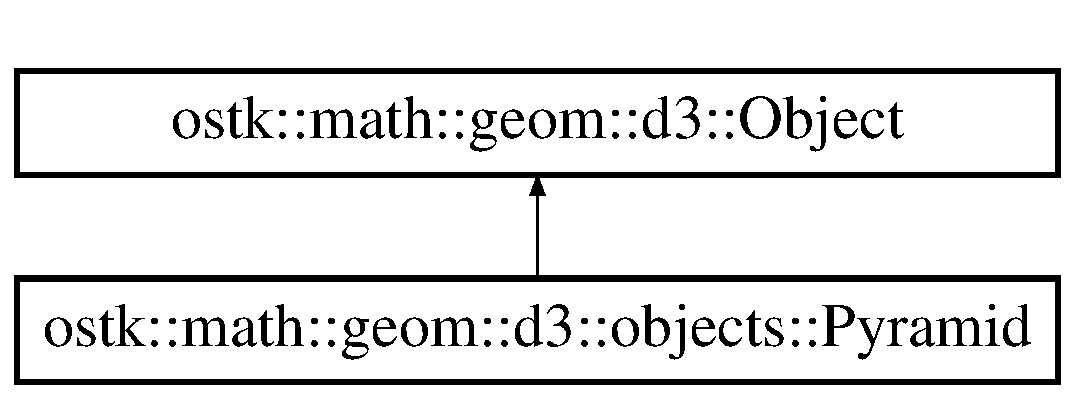
\includegraphics[height=2.000000cm]{classostk_1_1math_1_1geom_1_1d3_1_1objects_1_1_pyramid}
\end{center}
\end{figure}
\subsection*{Public Member Functions}
\begin{DoxyCompactItemize}
\item 
\hyperlink{classostk_1_1math_1_1geom_1_1d3_1_1objects_1_1_pyramid_a5560d123994714b36d4737b358dadcea}{Pyramid} (const \hyperlink{classostk_1_1math_1_1geom_1_1d3_1_1objects_1_1_polygon}{Polygon} \&a\+Base, const \hyperlink{classostk_1_1math_1_1geom_1_1d3_1_1objects_1_1_point}{Point} \&an\+Apex)
\begin{DoxyCompactList}\small\item\em Constructor. \end{DoxyCompactList}\item 
virtual \hyperlink{classostk_1_1math_1_1geom_1_1d3_1_1objects_1_1_pyramid}{Pyramid} $\ast$ \hyperlink{classostk_1_1math_1_1geom_1_1d3_1_1objects_1_1_pyramid_aefdaacc9298ef9d9a26137b2976f7dc6}{clone} () const override
\begin{DoxyCompactList}\small\item\em Clone pyramid. \end{DoxyCompactList}\item 
bool \hyperlink{classostk_1_1math_1_1geom_1_1d3_1_1objects_1_1_pyramid_a9385744e89111818c847fb440ae66ba4}{operator==} (const \hyperlink{classostk_1_1math_1_1geom_1_1d3_1_1objects_1_1_pyramid}{Pyramid} \&a\+Pyramid) const
\begin{DoxyCompactList}\small\item\em Equal to operator. \end{DoxyCompactList}\item 
bool \hyperlink{classostk_1_1math_1_1geom_1_1d3_1_1objects_1_1_pyramid_a413a5250a7dc5530f7e4321ca94648f8}{operator!=} (const \hyperlink{classostk_1_1math_1_1geom_1_1d3_1_1objects_1_1_pyramid}{Pyramid} \&a\+Pyramid) const
\begin{DoxyCompactList}\small\item\em Not equal to operator. \end{DoxyCompactList}\item 
virtual bool \hyperlink{classostk_1_1math_1_1geom_1_1d3_1_1objects_1_1_pyramid_acc4a62a7b5e51b6ad636638ca1c15504}{is\+Defined} () const override
\begin{DoxyCompactList}\small\item\em Check if pyramid is defined. \end{DoxyCompactList}\item 
bool \hyperlink{classostk_1_1math_1_1geom_1_1d3_1_1objects_1_1_pyramid_afec0e69f5caed5b0b676d70f414142dd}{intersects} (const \hyperlink{classostk_1_1math_1_1geom_1_1d3_1_1objects_1_1_sphere}{Sphere} \&a\+Sphere, const Size a\+Discretization\+Level=\hyperlink{_pyramid_8hpp_a3eb9931e85ba4c9718113211e549e91d}{D\+E\+F\+A\+U\+L\+T\+\_\+\+D\+I\+S\+C\+R\+E\+T\+I\+Z\+A\+T\+I\+O\+N\+\_\+\+L\+E\+V\+EL}) const
\begin{DoxyCompactList}\small\item\em Check if pyramid intersects sphere. \end{DoxyCompactList}\item 
bool \hyperlink{classostk_1_1math_1_1geom_1_1d3_1_1objects_1_1_pyramid_a807b60d75b73a97647cb41866c31e672}{intersects} (const \hyperlink{classostk_1_1math_1_1geom_1_1d3_1_1objects_1_1_ellipsoid}{Ellipsoid} \&an\+Ellipsoid, const Size a\+Discretization\+Level=\hyperlink{_pyramid_8hpp_a3eb9931e85ba4c9718113211e549e91d}{D\+E\+F\+A\+U\+L\+T\+\_\+\+D\+I\+S\+C\+R\+E\+T\+I\+Z\+A\+T\+I\+O\+N\+\_\+\+L\+E\+V\+EL}) const
\begin{DoxyCompactList}\small\item\em Check if pyramid intersects ellipsoid. \end{DoxyCompactList}\item 
bool \hyperlink{classostk_1_1math_1_1geom_1_1d3_1_1objects_1_1_pyramid_a7f476c37cc3f014bdc24e7fa4f2da743}{contains} (const \hyperlink{classostk_1_1math_1_1geom_1_1d3_1_1objects_1_1_point}{Point} \&a\+Point) const
\begin{DoxyCompactList}\small\item\em Check if pyramid contains point. \end{DoxyCompactList}\item 
bool \hyperlink{classostk_1_1math_1_1geom_1_1d3_1_1objects_1_1_pyramid_a4eebfb0cbd8d60ffce7db9b61b550e63}{contains} (const \hyperlink{classostk_1_1math_1_1geom_1_1d3_1_1objects_1_1_point_set}{Point\+Set} \&a\+Point\+Set) const
\begin{DoxyCompactList}\small\item\em Check if pyramid contains point set. \end{DoxyCompactList}\item 
bool \hyperlink{classostk_1_1math_1_1geom_1_1d3_1_1objects_1_1_pyramid_a7c7d10a2e8fb4a1b23a3b55a5156e588}{contains} (const \hyperlink{classostk_1_1math_1_1geom_1_1d3_1_1objects_1_1_segment}{Segment} \&a\+Segment) const
\begin{DoxyCompactList}\small\item\em Check if pyramid contains segment. \end{DoxyCompactList}\item 
bool \hyperlink{classostk_1_1math_1_1geom_1_1d3_1_1objects_1_1_pyramid_a761592bada278f4a80f910e3e234fde8}{contains} (const \hyperlink{classostk_1_1math_1_1geom_1_1d3_1_1objects_1_1_ellipsoid}{Ellipsoid} \&an\+Ellipsoid) const
\begin{DoxyCompactList}\small\item\em Check if pyramid contains ellipsoid. \end{DoxyCompactList}\item 
\hyperlink{classostk_1_1math_1_1geom_1_1d3_1_1objects_1_1_polygon}{Polygon} \hyperlink{classostk_1_1math_1_1geom_1_1d3_1_1objects_1_1_pyramid_ae1f35fb024a1cd171b750170cb1df0a4}{get\+Base} () const
\begin{DoxyCompactList}\small\item\em Get pyramid base. \end{DoxyCompactList}\item 
\hyperlink{classostk_1_1math_1_1geom_1_1d3_1_1objects_1_1_point}{Point} \hyperlink{classostk_1_1math_1_1geom_1_1d3_1_1objects_1_1_pyramid_acbc557f7d8bbfe1fc3f59fdad16684a3}{get\+Apex} () const
\begin{DoxyCompactList}\small\item\em Get pyramid apex. \end{DoxyCompactList}\item 
Size \hyperlink{classostk_1_1math_1_1geom_1_1d3_1_1objects_1_1_pyramid_af853f40f9b9501c7fcad30337d646c4c}{get\+Lateral\+Face\+Count} () const
\begin{DoxyCompactList}\small\item\em Get number of lateral faces. \end{DoxyCompactList}\item 
\hyperlink{classostk_1_1math_1_1geom_1_1d3_1_1objects_1_1_polygon}{Polygon} \hyperlink{classostk_1_1math_1_1geom_1_1d3_1_1objects_1_1_pyramid_a5c29f2b5915fbcf7a200b49840805c86}{get\+Lateral\+Face\+At} (const Index a\+Lateral\+Face\+Index) const
\begin{DoxyCompactList}\small\item\em Get lateral face at index. \end{DoxyCompactList}\item 
Array$<$ \hyperlink{classostk_1_1math_1_1geom_1_1d3_1_1objects_1_1_ray}{Ray} $>$ \hyperlink{classostk_1_1math_1_1geom_1_1d3_1_1objects_1_1_pyramid_a798481e060dc0af1ed8ed57a75d8fa9b}{get\+Rays\+Of\+Lateral\+Face\+At} (const Index a\+Lateral\+Face\+Index, const Size a\+Ray\+Count=2) const
\begin{DoxyCompactList}\small\item\em Get rays of lateral face at index. \end{DoxyCompactList}\item 
Array$<$ \hyperlink{classostk_1_1math_1_1geom_1_1d3_1_1objects_1_1_ray}{Ray} $>$ \hyperlink{classostk_1_1math_1_1geom_1_1d3_1_1objects_1_1_pyramid_a7ead70ef5dff894a705f337dbc6cbff6}{get\+Rays\+Of\+Lateral\+Faces} (const Size a\+Ray\+Count=0) const
\begin{DoxyCompactList}\small\item\em Get rays of lateral faces. \end{DoxyCompactList}\item 
\hyperlink{classostk_1_1math_1_1geom_1_1d3_1_1_intersection}{Intersection} \hyperlink{classostk_1_1math_1_1geom_1_1d3_1_1objects_1_1_pyramid_a254b6d83bb83794852fe13317728ddf0}{intersection\+With} (const \hyperlink{classostk_1_1math_1_1geom_1_1d3_1_1objects_1_1_sphere}{Sphere} \&a\+Sphere, const bool only\+In\+Sight=\hyperlink{_sphere_8hpp_af424617f7c785f4835e2feba5a5640f2}{D\+E\+F\+A\+U\+L\+T\+\_\+\+O\+N\+L\+Y\+\_\+\+I\+N\+\_\+\+S\+I\+G\+HT}, const Size a\+Discretization\+Level=\hyperlink{_pyramid_8hpp_a3eb9931e85ba4c9718113211e549e91d}{D\+E\+F\+A\+U\+L\+T\+\_\+\+D\+I\+S\+C\+R\+E\+T\+I\+Z\+A\+T\+I\+O\+N\+\_\+\+L\+E\+V\+EL}) const
\begin{DoxyCompactList}\small\item\em Compute intersection of pyramid with sphere. \end{DoxyCompactList}\item 
\hyperlink{classostk_1_1math_1_1geom_1_1d3_1_1_intersection}{Intersection} \hyperlink{classostk_1_1math_1_1geom_1_1d3_1_1objects_1_1_pyramid_aedc018303c7b9788036bc9269fcc161f}{intersection\+With} (const \hyperlink{classostk_1_1math_1_1geom_1_1d3_1_1objects_1_1_ellipsoid}{Ellipsoid} \&an\+Ellipsoid, const bool only\+In\+Sight=\hyperlink{_sphere_8hpp_af424617f7c785f4835e2feba5a5640f2}{D\+E\+F\+A\+U\+L\+T\+\_\+\+O\+N\+L\+Y\+\_\+\+I\+N\+\_\+\+S\+I\+G\+HT}, const Size a\+Discretization\+Level=\hyperlink{_pyramid_8hpp_a3eb9931e85ba4c9718113211e549e91d}{D\+E\+F\+A\+U\+L\+T\+\_\+\+D\+I\+S\+C\+R\+E\+T\+I\+Z\+A\+T\+I\+O\+N\+\_\+\+L\+E\+V\+EL}) const
\begin{DoxyCompactList}\small\item\em Compute intersection of pyramid with ellipsoid. \end{DoxyCompactList}\item 
virtual void \hyperlink{classostk_1_1math_1_1geom_1_1d3_1_1objects_1_1_pyramid_ae308eee53a721c8c41463a1ec4842a2d}{print} (std\+::ostream \&an\+Output\+Stream, bool display\+Decorators=true) const override
\begin{DoxyCompactList}\small\item\em Print pyramid. \end{DoxyCompactList}\item 
virtual void \hyperlink{classostk_1_1math_1_1geom_1_1d3_1_1objects_1_1_pyramid_ab4f31049019c0ea4b87931adf4ba7c5d}{apply\+Transformation} (const \hyperlink{classostk_1_1math_1_1geom_1_1d3_1_1_transformation}{Transformation} \&a\+Transformation) override
\begin{DoxyCompactList}\small\item\em Apply transformation to pyramid. \end{DoxyCompactList}\end{DoxyCompactItemize}
\subsection*{Static Public Member Functions}
\begin{DoxyCompactItemize}
\item 
static \hyperlink{classostk_1_1math_1_1geom_1_1d3_1_1objects_1_1_pyramid}{Pyramid} \hyperlink{classostk_1_1math_1_1geom_1_1d3_1_1objects_1_1_pyramid_a1da403f46a6f5566358d74b633478135}{Undefined} ()
\begin{DoxyCompactList}\small\item\em Constructs an undefined pyramid. \end{DoxyCompactList}\end{DoxyCompactItemize}


\subsection{Detailed Description}
\hyperlink{classostk_1_1math_1_1geom_1_1d3_1_1objects_1_1_pyramid}{Pyramid}. 

A pyramid is a polyhedron formed by connecting a polygonal base and a point, called the apex. Each base edge and apex form a triangle, called a lateral face.

https\+://en.wikipedia.\+org/wiki/\+Pyramid\+\_\+(geometry) 

\subsection{Constructor \& Destructor Documentation}
\mbox{\Hypertarget{classostk_1_1math_1_1geom_1_1d3_1_1objects_1_1_pyramid_a5560d123994714b36d4737b358dadcea}\label{classostk_1_1math_1_1geom_1_1d3_1_1objects_1_1_pyramid_a5560d123994714b36d4737b358dadcea}} 
\index{ostk\+::math\+::geom\+::d3\+::objects\+::\+Pyramid@{ostk\+::math\+::geom\+::d3\+::objects\+::\+Pyramid}!Pyramid@{Pyramid}}
\index{Pyramid@{Pyramid}!ostk\+::math\+::geom\+::d3\+::objects\+::\+Pyramid@{ostk\+::math\+::geom\+::d3\+::objects\+::\+Pyramid}}
\subsubsection{\texorpdfstring{Pyramid()}{Pyramid()}}
{\footnotesize\ttfamily ostk\+::math\+::geom\+::d3\+::objects\+::\+Pyramid\+::\+Pyramid (\begin{DoxyParamCaption}\item[{const \hyperlink{classostk_1_1math_1_1geom_1_1d3_1_1objects_1_1_polygon}{Polygon} \&}]{a\+Base,  }\item[{const \hyperlink{classostk_1_1math_1_1geom_1_1d3_1_1objects_1_1_point}{Point} \&}]{an\+Apex }\end{DoxyParamCaption})}



Constructor. 


\begin{DoxyCode}
Polygon base = ... ;
Point apex = \{ 0.0, 0.0, 1.0 \} ;
\hyperlink{classostk_1_1math_1_1geom_1_1d3_1_1objects_1_1_pyramid_a5560d123994714b36d4737b358dadcea}{Pyramid} pyramid = \{ base, apex \} ;
\end{DoxyCode}



\begin{DoxyParams}[1]{Parameters}
\mbox{\tt in}  & {\em a\+Base} & A pyramid base \\
\hline
\mbox{\tt in}  & {\em an\+Apex} & A pyramid apex \\
\hline
\end{DoxyParams}


\subsection{Member Function Documentation}
\mbox{\Hypertarget{classostk_1_1math_1_1geom_1_1d3_1_1objects_1_1_pyramid_ab4f31049019c0ea4b87931adf4ba7c5d}\label{classostk_1_1math_1_1geom_1_1d3_1_1objects_1_1_pyramid_ab4f31049019c0ea4b87931adf4ba7c5d}} 
\index{ostk\+::math\+::geom\+::d3\+::objects\+::\+Pyramid@{ostk\+::math\+::geom\+::d3\+::objects\+::\+Pyramid}!apply\+Transformation@{apply\+Transformation}}
\index{apply\+Transformation@{apply\+Transformation}!ostk\+::math\+::geom\+::d3\+::objects\+::\+Pyramid@{ostk\+::math\+::geom\+::d3\+::objects\+::\+Pyramid}}
\subsubsection{\texorpdfstring{apply\+Transformation()}{applyTransformation()}}
{\footnotesize\ttfamily void ostk\+::math\+::geom\+::d3\+::objects\+::\+Pyramid\+::apply\+Transformation (\begin{DoxyParamCaption}\item[{const \hyperlink{classostk_1_1math_1_1geom_1_1d3_1_1_transformation}{Transformation} \&}]{a\+Transformation }\end{DoxyParamCaption})\hspace{0.3cm}{\ttfamily [override]}, {\ttfamily [virtual]}}



Apply transformation to pyramid. 


\begin{DoxyParams}[1]{Parameters}
\mbox{\tt in}  & {\em a\+Transformation} & A transformation \\
\hline
\end{DoxyParams}


Implements \hyperlink{classostk_1_1math_1_1geom_1_1d3_1_1_object_ae9194dd6d2bb4df09292ffc84dccdb1d}{ostk\+::math\+::geom\+::d3\+::\+Object}.

\mbox{\Hypertarget{classostk_1_1math_1_1geom_1_1d3_1_1objects_1_1_pyramid_aefdaacc9298ef9d9a26137b2976f7dc6}\label{classostk_1_1math_1_1geom_1_1d3_1_1objects_1_1_pyramid_aefdaacc9298ef9d9a26137b2976f7dc6}} 
\index{ostk\+::math\+::geom\+::d3\+::objects\+::\+Pyramid@{ostk\+::math\+::geom\+::d3\+::objects\+::\+Pyramid}!clone@{clone}}
\index{clone@{clone}!ostk\+::math\+::geom\+::d3\+::objects\+::\+Pyramid@{ostk\+::math\+::geom\+::d3\+::objects\+::\+Pyramid}}
\subsubsection{\texorpdfstring{clone()}{clone()}}
{\footnotesize\ttfamily \hyperlink{classostk_1_1math_1_1geom_1_1d3_1_1objects_1_1_pyramid}{Pyramid} $\ast$ ostk\+::math\+::geom\+::d3\+::objects\+::\+Pyramid\+::clone (\begin{DoxyParamCaption}{ }\end{DoxyParamCaption}) const\hspace{0.3cm}{\ttfamily [override]}, {\ttfamily [virtual]}}



Clone pyramid. 

\begin{DoxyReturn}{Returns}
Pointer to cloned pyramid 
\end{DoxyReturn}


Implements \hyperlink{classostk_1_1math_1_1geom_1_1d3_1_1_object_a676013f9555f6492687f9809b2db887b}{ostk\+::math\+::geom\+::d3\+::\+Object}.

\mbox{\Hypertarget{classostk_1_1math_1_1geom_1_1d3_1_1objects_1_1_pyramid_a7f476c37cc3f014bdc24e7fa4f2da743}\label{classostk_1_1math_1_1geom_1_1d3_1_1objects_1_1_pyramid_a7f476c37cc3f014bdc24e7fa4f2da743}} 
\index{ostk\+::math\+::geom\+::d3\+::objects\+::\+Pyramid@{ostk\+::math\+::geom\+::d3\+::objects\+::\+Pyramid}!contains@{contains}}
\index{contains@{contains}!ostk\+::math\+::geom\+::d3\+::objects\+::\+Pyramid@{ostk\+::math\+::geom\+::d3\+::objects\+::\+Pyramid}}
\subsubsection{\texorpdfstring{contains()}{contains()}\hspace{0.1cm}{\footnotesize\ttfamily [1/4]}}
{\footnotesize\ttfamily bool ostk\+::math\+::geom\+::d3\+::objects\+::\+Pyramid\+::contains (\begin{DoxyParamCaption}\item[{const \hyperlink{classostk_1_1math_1_1geom_1_1d3_1_1objects_1_1_point}{Point} \&}]{a\+Point }\end{DoxyParamCaption}) const}



Check if pyramid contains point. 


\begin{DoxyCode}
\hyperlink{classostk_1_1math_1_1geom_1_1d3_1_1objects_1_1_pyramid_a5560d123994714b36d4737b358dadcea}{Pyramid} pyramid = ... ;
Point point = ... ;
pyramid.contains(point) ;
\end{DoxyCode}



\begin{DoxyParams}[1]{Parameters}
\mbox{\tt in}  & {\em a\+Point} & A point \\
\hline
\end{DoxyParams}
\begin{DoxyReturn}{Returns}
True if pyramid contains point 
\end{DoxyReturn}
\mbox{\Hypertarget{classostk_1_1math_1_1geom_1_1d3_1_1objects_1_1_pyramid_a4eebfb0cbd8d60ffce7db9b61b550e63}\label{classostk_1_1math_1_1geom_1_1d3_1_1objects_1_1_pyramid_a4eebfb0cbd8d60ffce7db9b61b550e63}} 
\index{ostk\+::math\+::geom\+::d3\+::objects\+::\+Pyramid@{ostk\+::math\+::geom\+::d3\+::objects\+::\+Pyramid}!contains@{contains}}
\index{contains@{contains}!ostk\+::math\+::geom\+::d3\+::objects\+::\+Pyramid@{ostk\+::math\+::geom\+::d3\+::objects\+::\+Pyramid}}
\subsubsection{\texorpdfstring{contains()}{contains()}\hspace{0.1cm}{\footnotesize\ttfamily [2/4]}}
{\footnotesize\ttfamily bool ostk\+::math\+::geom\+::d3\+::objects\+::\+Pyramid\+::contains (\begin{DoxyParamCaption}\item[{const \hyperlink{classostk_1_1math_1_1geom_1_1d3_1_1objects_1_1_point_set}{Point\+Set} \&}]{a\+Point\+Set }\end{DoxyParamCaption}) const}



Check if pyramid contains point set. 


\begin{DoxyCode}
\hyperlink{classostk_1_1math_1_1geom_1_1d3_1_1objects_1_1_pyramid_a5560d123994714b36d4737b358dadcea}{Pyramid} pyramid = ... ;
PointSet pointSet = ... ;
pyramid.contains(pointSet) ;
\end{DoxyCode}



\begin{DoxyParams}[1]{Parameters}
\mbox{\tt in}  & {\em a\+Point\+Set} & A point set \\
\hline
\end{DoxyParams}
\begin{DoxyReturn}{Returns}
True if pyramid contains point set 
\end{DoxyReturn}
\mbox{\Hypertarget{classostk_1_1math_1_1geom_1_1d3_1_1objects_1_1_pyramid_a7c7d10a2e8fb4a1b23a3b55a5156e588}\label{classostk_1_1math_1_1geom_1_1d3_1_1objects_1_1_pyramid_a7c7d10a2e8fb4a1b23a3b55a5156e588}} 
\index{ostk\+::math\+::geom\+::d3\+::objects\+::\+Pyramid@{ostk\+::math\+::geom\+::d3\+::objects\+::\+Pyramid}!contains@{contains}}
\index{contains@{contains}!ostk\+::math\+::geom\+::d3\+::objects\+::\+Pyramid@{ostk\+::math\+::geom\+::d3\+::objects\+::\+Pyramid}}
\subsubsection{\texorpdfstring{contains()}{contains()}\hspace{0.1cm}{\footnotesize\ttfamily [3/4]}}
{\footnotesize\ttfamily bool ostk\+::math\+::geom\+::d3\+::objects\+::\+Pyramid\+::contains (\begin{DoxyParamCaption}\item[{const \hyperlink{classostk_1_1math_1_1geom_1_1d3_1_1objects_1_1_segment}{Segment} \&}]{a\+Segment }\end{DoxyParamCaption}) const}



Check if pyramid contains segment. 


\begin{DoxyCode}
\hyperlink{classostk_1_1math_1_1geom_1_1d3_1_1objects_1_1_pyramid_a5560d123994714b36d4737b358dadcea}{Pyramid} pyramid = ... ;
Segment segment = ... ;
pyramid.contains(segment) ;
\end{DoxyCode}



\begin{DoxyParams}[1]{Parameters}
\mbox{\tt in}  & {\em a\+Segment} & A segment \\
\hline
\end{DoxyParams}
\begin{DoxyReturn}{Returns}
True if pyramid contains segment 
\end{DoxyReturn}
\mbox{\Hypertarget{classostk_1_1math_1_1geom_1_1d3_1_1objects_1_1_pyramid_a761592bada278f4a80f910e3e234fde8}\label{classostk_1_1math_1_1geom_1_1d3_1_1objects_1_1_pyramid_a761592bada278f4a80f910e3e234fde8}} 
\index{ostk\+::math\+::geom\+::d3\+::objects\+::\+Pyramid@{ostk\+::math\+::geom\+::d3\+::objects\+::\+Pyramid}!contains@{contains}}
\index{contains@{contains}!ostk\+::math\+::geom\+::d3\+::objects\+::\+Pyramid@{ostk\+::math\+::geom\+::d3\+::objects\+::\+Pyramid}}
\subsubsection{\texorpdfstring{contains()}{contains()}\hspace{0.1cm}{\footnotesize\ttfamily [4/4]}}
{\footnotesize\ttfamily bool ostk\+::math\+::geom\+::d3\+::objects\+::\+Pyramid\+::contains (\begin{DoxyParamCaption}\item[{const \hyperlink{classostk_1_1math_1_1geom_1_1d3_1_1objects_1_1_ellipsoid}{Ellipsoid} \&}]{an\+Ellipsoid }\end{DoxyParamCaption}) const}



Check if pyramid contains ellipsoid. 


\begin{DoxyCode}
\hyperlink{classostk_1_1math_1_1geom_1_1d3_1_1objects_1_1_pyramid_a5560d123994714b36d4737b358dadcea}{Pyramid} pyramid = ... ;
Ellipsoid ellipsoid = ... ;
pyramid.contains(ellipsoid) ;
\end{DoxyCode}



\begin{DoxyParams}[1]{Parameters}
\mbox{\tt in}  & {\em an\+Ellipsoid} & An ellipsoid \\
\hline
\end{DoxyParams}
\begin{DoxyReturn}{Returns}
True if pyramid contains ellipsoid 
\end{DoxyReturn}
\mbox{\Hypertarget{classostk_1_1math_1_1geom_1_1d3_1_1objects_1_1_pyramid_acbc557f7d8bbfe1fc3f59fdad16684a3}\label{classostk_1_1math_1_1geom_1_1d3_1_1objects_1_1_pyramid_acbc557f7d8bbfe1fc3f59fdad16684a3}} 
\index{ostk\+::math\+::geom\+::d3\+::objects\+::\+Pyramid@{ostk\+::math\+::geom\+::d3\+::objects\+::\+Pyramid}!get\+Apex@{get\+Apex}}
\index{get\+Apex@{get\+Apex}!ostk\+::math\+::geom\+::d3\+::objects\+::\+Pyramid@{ostk\+::math\+::geom\+::d3\+::objects\+::\+Pyramid}}
\subsubsection{\texorpdfstring{get\+Apex()}{getApex()}}
{\footnotesize\ttfamily \hyperlink{classostk_1_1math_1_1geom_1_1d3_1_1objects_1_1_point}{Point} ostk\+::math\+::geom\+::d3\+::objects\+::\+Pyramid\+::get\+Apex (\begin{DoxyParamCaption}{ }\end{DoxyParamCaption}) const}



Get pyramid apex. 

\begin{DoxyReturn}{Returns}
\hyperlink{classostk_1_1math_1_1geom_1_1d3_1_1objects_1_1_pyramid}{Pyramid} apex 
\end{DoxyReturn}
\mbox{\Hypertarget{classostk_1_1math_1_1geom_1_1d3_1_1objects_1_1_pyramid_ae1f35fb024a1cd171b750170cb1df0a4}\label{classostk_1_1math_1_1geom_1_1d3_1_1objects_1_1_pyramid_ae1f35fb024a1cd171b750170cb1df0a4}} 
\index{ostk\+::math\+::geom\+::d3\+::objects\+::\+Pyramid@{ostk\+::math\+::geom\+::d3\+::objects\+::\+Pyramid}!get\+Base@{get\+Base}}
\index{get\+Base@{get\+Base}!ostk\+::math\+::geom\+::d3\+::objects\+::\+Pyramid@{ostk\+::math\+::geom\+::d3\+::objects\+::\+Pyramid}}
\subsubsection{\texorpdfstring{get\+Base()}{getBase()}}
{\footnotesize\ttfamily \hyperlink{classostk_1_1math_1_1geom_1_1d3_1_1objects_1_1_polygon}{Polygon} ostk\+::math\+::geom\+::d3\+::objects\+::\+Pyramid\+::get\+Base (\begin{DoxyParamCaption}{ }\end{DoxyParamCaption}) const}



Get pyramid base. 

\begin{DoxyReturn}{Returns}
\hyperlink{classostk_1_1math_1_1geom_1_1d3_1_1objects_1_1_pyramid}{Pyramid} base 
\end{DoxyReturn}
\mbox{\Hypertarget{classostk_1_1math_1_1geom_1_1d3_1_1objects_1_1_pyramid_a5c29f2b5915fbcf7a200b49840805c86}\label{classostk_1_1math_1_1geom_1_1d3_1_1objects_1_1_pyramid_a5c29f2b5915fbcf7a200b49840805c86}} 
\index{ostk\+::math\+::geom\+::d3\+::objects\+::\+Pyramid@{ostk\+::math\+::geom\+::d3\+::objects\+::\+Pyramid}!get\+Lateral\+Face\+At@{get\+Lateral\+Face\+At}}
\index{get\+Lateral\+Face\+At@{get\+Lateral\+Face\+At}!ostk\+::math\+::geom\+::d3\+::objects\+::\+Pyramid@{ostk\+::math\+::geom\+::d3\+::objects\+::\+Pyramid}}
\subsubsection{\texorpdfstring{get\+Lateral\+Face\+At()}{getLateralFaceAt()}}
{\footnotesize\ttfamily \hyperlink{classostk_1_1math_1_1geom_1_1d3_1_1objects_1_1_polygon}{Polygon} ostk\+::math\+::geom\+::d3\+::objects\+::\+Pyramid\+::get\+Lateral\+Face\+At (\begin{DoxyParamCaption}\item[{const Index}]{a\+Lateral\+Face\+Index }\end{DoxyParamCaption}) const}



Get lateral face at index. 


\begin{DoxyParams}[1]{Parameters}
\mbox{\tt in}  & {\em a\+Lateral\+Face\+Index} & A lateral face index \\
\hline
\end{DoxyParams}
\begin{DoxyReturn}{Returns}
Lateral face 
\end{DoxyReturn}
\mbox{\Hypertarget{classostk_1_1math_1_1geom_1_1d3_1_1objects_1_1_pyramid_af853f40f9b9501c7fcad30337d646c4c}\label{classostk_1_1math_1_1geom_1_1d3_1_1objects_1_1_pyramid_af853f40f9b9501c7fcad30337d646c4c}} 
\index{ostk\+::math\+::geom\+::d3\+::objects\+::\+Pyramid@{ostk\+::math\+::geom\+::d3\+::objects\+::\+Pyramid}!get\+Lateral\+Face\+Count@{get\+Lateral\+Face\+Count}}
\index{get\+Lateral\+Face\+Count@{get\+Lateral\+Face\+Count}!ostk\+::math\+::geom\+::d3\+::objects\+::\+Pyramid@{ostk\+::math\+::geom\+::d3\+::objects\+::\+Pyramid}}
\subsubsection{\texorpdfstring{get\+Lateral\+Face\+Count()}{getLateralFaceCount()}}
{\footnotesize\ttfamily Size ostk\+::math\+::geom\+::d3\+::objects\+::\+Pyramid\+::get\+Lateral\+Face\+Count (\begin{DoxyParamCaption}{ }\end{DoxyParamCaption}) const}



Get number of lateral faces. 

\begin{DoxyReturn}{Returns}
Number of lateral faces 
\end{DoxyReturn}
\mbox{\Hypertarget{classostk_1_1math_1_1geom_1_1d3_1_1objects_1_1_pyramid_a798481e060dc0af1ed8ed57a75d8fa9b}\label{classostk_1_1math_1_1geom_1_1d3_1_1objects_1_1_pyramid_a798481e060dc0af1ed8ed57a75d8fa9b}} 
\index{ostk\+::math\+::geom\+::d3\+::objects\+::\+Pyramid@{ostk\+::math\+::geom\+::d3\+::objects\+::\+Pyramid}!get\+Rays\+Of\+Lateral\+Face\+At@{get\+Rays\+Of\+Lateral\+Face\+At}}
\index{get\+Rays\+Of\+Lateral\+Face\+At@{get\+Rays\+Of\+Lateral\+Face\+At}!ostk\+::math\+::geom\+::d3\+::objects\+::\+Pyramid@{ostk\+::math\+::geom\+::d3\+::objects\+::\+Pyramid}}
\subsubsection{\texorpdfstring{get\+Rays\+Of\+Lateral\+Face\+At()}{getRaysOfLateralFaceAt()}}
{\footnotesize\ttfamily Array$<$ \hyperlink{classostk_1_1math_1_1geom_1_1d3_1_1objects_1_1_ray}{Ray} $>$ ostk\+::math\+::geom\+::d3\+::objects\+::\+Pyramid\+::get\+Rays\+Of\+Lateral\+Face\+At (\begin{DoxyParamCaption}\item[{const Index}]{a\+Lateral\+Face\+Index,  }\item[{const Size}]{a\+Ray\+Count = {\ttfamily 2} }\end{DoxyParamCaption}) const}



Get rays of lateral face at index. 


\begin{DoxyParams}[1]{Parameters}
\mbox{\tt in}  & {\em a\+Lateral\+Face\+Index} & A lateral face index \\
\hline
\mbox{\tt in}  & {\em a\+Ray\+Count} & A number of rays (at least 2) \\
\hline
\end{DoxyParams}
\begin{DoxyReturn}{Returns}
Array of rays 
\end{DoxyReturn}
\mbox{\Hypertarget{classostk_1_1math_1_1geom_1_1d3_1_1objects_1_1_pyramid_a7ead70ef5dff894a705f337dbc6cbff6}\label{classostk_1_1math_1_1geom_1_1d3_1_1objects_1_1_pyramid_a7ead70ef5dff894a705f337dbc6cbff6}} 
\index{ostk\+::math\+::geom\+::d3\+::objects\+::\+Pyramid@{ostk\+::math\+::geom\+::d3\+::objects\+::\+Pyramid}!get\+Rays\+Of\+Lateral\+Faces@{get\+Rays\+Of\+Lateral\+Faces}}
\index{get\+Rays\+Of\+Lateral\+Faces@{get\+Rays\+Of\+Lateral\+Faces}!ostk\+::math\+::geom\+::d3\+::objects\+::\+Pyramid@{ostk\+::math\+::geom\+::d3\+::objects\+::\+Pyramid}}
\subsubsection{\texorpdfstring{get\+Rays\+Of\+Lateral\+Faces()}{getRaysOfLateralFaces()}}
{\footnotesize\ttfamily Array$<$ \hyperlink{classostk_1_1math_1_1geom_1_1d3_1_1objects_1_1_ray}{Ray} $>$ ostk\+::math\+::geom\+::d3\+::objects\+::\+Pyramid\+::get\+Rays\+Of\+Lateral\+Faces (\begin{DoxyParamCaption}\item[{const Size}]{a\+Ray\+Count = {\ttfamily 0} }\end{DoxyParamCaption}) const}



Get rays of lateral faces. 


\begin{DoxyParams}[1]{Parameters}
\mbox{\tt in}  & {\em a\+Ray\+Count} & A number of rays (at least face count) \\
\hline
\end{DoxyParams}
\begin{DoxyReturn}{Returns}
Array of rays 
\end{DoxyReturn}
\mbox{\Hypertarget{classostk_1_1math_1_1geom_1_1d3_1_1objects_1_1_pyramid_a254b6d83bb83794852fe13317728ddf0}\label{classostk_1_1math_1_1geom_1_1d3_1_1objects_1_1_pyramid_a254b6d83bb83794852fe13317728ddf0}} 
\index{ostk\+::math\+::geom\+::d3\+::objects\+::\+Pyramid@{ostk\+::math\+::geom\+::d3\+::objects\+::\+Pyramid}!intersection\+With@{intersection\+With}}
\index{intersection\+With@{intersection\+With}!ostk\+::math\+::geom\+::d3\+::objects\+::\+Pyramid@{ostk\+::math\+::geom\+::d3\+::objects\+::\+Pyramid}}
\subsubsection{\texorpdfstring{intersection\+With()}{intersectionWith()}\hspace{0.1cm}{\footnotesize\ttfamily [1/2]}}
{\footnotesize\ttfamily \hyperlink{classostk_1_1math_1_1geom_1_1d3_1_1_intersection}{Intersection} ostk\+::math\+::geom\+::d3\+::objects\+::\+Pyramid\+::intersection\+With (\begin{DoxyParamCaption}\item[{const \hyperlink{classostk_1_1math_1_1geom_1_1d3_1_1objects_1_1_sphere}{Sphere} \&}]{a\+Sphere,  }\item[{const bool}]{only\+In\+Sight = {\ttfamily \hyperlink{_sphere_8hpp_af424617f7c785f4835e2feba5a5640f2}{D\+E\+F\+A\+U\+L\+T\+\_\+\+O\+N\+L\+Y\+\_\+\+I\+N\+\_\+\+S\+I\+G\+HT}},  }\item[{const Size}]{a\+Discretization\+Level = {\ttfamily \hyperlink{_pyramid_8hpp_a3eb9931e85ba4c9718113211e549e91d}{D\+E\+F\+A\+U\+L\+T\+\_\+\+D\+I\+S\+C\+R\+E\+T\+I\+Z\+A\+T\+I\+O\+N\+\_\+\+L\+E\+V\+EL}} }\end{DoxyParamCaption}) const}



Compute intersection of pyramid with sphere. 


\begin{DoxyParams}[1]{Parameters}
\mbox{\tt in}  & {\em a\+Sphere} & A sphere \\
\hline
\mbox{\tt in}  & {\em only\+In\+Sight} & (optional) If true, only return intersection points that are in sight \\
\hline
\mbox{\tt in}  & {\em a\+Discretization\+Level} & (optional) The polygonal discretization level \\
\hline
\end{DoxyParams}
\begin{DoxyReturn}{Returns}
\hyperlink{classostk_1_1math_1_1geom_1_1d3_1_1_intersection}{Intersection} of pyramid with sphere 
\end{DoxyReturn}
\mbox{\Hypertarget{classostk_1_1math_1_1geom_1_1d3_1_1objects_1_1_pyramid_aedc018303c7b9788036bc9269fcc161f}\label{classostk_1_1math_1_1geom_1_1d3_1_1objects_1_1_pyramid_aedc018303c7b9788036bc9269fcc161f}} 
\index{ostk\+::math\+::geom\+::d3\+::objects\+::\+Pyramid@{ostk\+::math\+::geom\+::d3\+::objects\+::\+Pyramid}!intersection\+With@{intersection\+With}}
\index{intersection\+With@{intersection\+With}!ostk\+::math\+::geom\+::d3\+::objects\+::\+Pyramid@{ostk\+::math\+::geom\+::d3\+::objects\+::\+Pyramid}}
\subsubsection{\texorpdfstring{intersection\+With()}{intersectionWith()}\hspace{0.1cm}{\footnotesize\ttfamily [2/2]}}
{\footnotesize\ttfamily \hyperlink{classostk_1_1math_1_1geom_1_1d3_1_1_intersection}{Intersection} ostk\+::math\+::geom\+::d3\+::objects\+::\+Pyramid\+::intersection\+With (\begin{DoxyParamCaption}\item[{const \hyperlink{classostk_1_1math_1_1geom_1_1d3_1_1objects_1_1_ellipsoid}{Ellipsoid} \&}]{an\+Ellipsoid,  }\item[{const bool}]{only\+In\+Sight = {\ttfamily \hyperlink{_sphere_8hpp_af424617f7c785f4835e2feba5a5640f2}{D\+E\+F\+A\+U\+L\+T\+\_\+\+O\+N\+L\+Y\+\_\+\+I\+N\+\_\+\+S\+I\+G\+HT}},  }\item[{const Size}]{a\+Discretization\+Level = {\ttfamily \hyperlink{_pyramid_8hpp_a3eb9931e85ba4c9718113211e549e91d}{D\+E\+F\+A\+U\+L\+T\+\_\+\+D\+I\+S\+C\+R\+E\+T\+I\+Z\+A\+T\+I\+O\+N\+\_\+\+L\+E\+V\+EL}} }\end{DoxyParamCaption}) const}



Compute intersection of pyramid with ellipsoid. 


\begin{DoxyParams}[1]{Parameters}
\mbox{\tt in}  & {\em an\+Ellipsoid} & An ellipsoid \\
\hline
\mbox{\tt in}  & {\em only\+In\+Sight} & (optional) If true, only return intersection points that are in sight \\
\hline
\mbox{\tt in}  & {\em a\+Discretization\+Level} & (optional) The polygonal discretization level \\
\hline
\end{DoxyParams}
\begin{DoxyReturn}{Returns}
\hyperlink{classostk_1_1math_1_1geom_1_1d3_1_1_intersection}{Intersection} of pyramid with ellipsoid 
\end{DoxyReturn}
\mbox{\Hypertarget{classostk_1_1math_1_1geom_1_1d3_1_1objects_1_1_pyramid_afec0e69f5caed5b0b676d70f414142dd}\label{classostk_1_1math_1_1geom_1_1d3_1_1objects_1_1_pyramid_afec0e69f5caed5b0b676d70f414142dd}} 
\index{ostk\+::math\+::geom\+::d3\+::objects\+::\+Pyramid@{ostk\+::math\+::geom\+::d3\+::objects\+::\+Pyramid}!intersects@{intersects}}
\index{intersects@{intersects}!ostk\+::math\+::geom\+::d3\+::objects\+::\+Pyramid@{ostk\+::math\+::geom\+::d3\+::objects\+::\+Pyramid}}
\subsubsection{\texorpdfstring{intersects()}{intersects()}\hspace{0.1cm}{\footnotesize\ttfamily [1/2]}}
{\footnotesize\ttfamily bool ostk\+::math\+::geom\+::d3\+::objects\+::\+Pyramid\+::intersects (\begin{DoxyParamCaption}\item[{const \hyperlink{classostk_1_1math_1_1geom_1_1d3_1_1objects_1_1_sphere}{Sphere} \&}]{a\+Sphere,  }\item[{const Size}]{a\+Discretization\+Level = {\ttfamily \hyperlink{_pyramid_8hpp_a3eb9931e85ba4c9718113211e549e91d}{D\+E\+F\+A\+U\+L\+T\+\_\+\+D\+I\+S\+C\+R\+E\+T\+I\+Z\+A\+T\+I\+O\+N\+\_\+\+L\+E\+V\+EL}} }\end{DoxyParamCaption}) const}



Check if pyramid intersects sphere. 


\begin{DoxyCode}
\hyperlink{classostk_1_1math_1_1geom_1_1d3_1_1objects_1_1_pyramid_a5560d123994714b36d4737b358dadcea}{Pyramid} pyramid = ... ;
Sphere sphere = ... ;
pyramid.intersects(sphere) ;
\end{DoxyCode}



\begin{DoxyParams}[1]{Parameters}
\mbox{\tt in}  & {\em a\+Sphere} & A sphere \\
\hline
\mbox{\tt in}  & {\em a\+Discretization\+Level} & (optional) The polygonal discretization level \\
\hline
\end{DoxyParams}
\begin{DoxyReturn}{Returns}
True if pyramid intersects sphere 
\end{DoxyReturn}
\mbox{\Hypertarget{classostk_1_1math_1_1geom_1_1d3_1_1objects_1_1_pyramid_a807b60d75b73a97647cb41866c31e672}\label{classostk_1_1math_1_1geom_1_1d3_1_1objects_1_1_pyramid_a807b60d75b73a97647cb41866c31e672}} 
\index{ostk\+::math\+::geom\+::d3\+::objects\+::\+Pyramid@{ostk\+::math\+::geom\+::d3\+::objects\+::\+Pyramid}!intersects@{intersects}}
\index{intersects@{intersects}!ostk\+::math\+::geom\+::d3\+::objects\+::\+Pyramid@{ostk\+::math\+::geom\+::d3\+::objects\+::\+Pyramid}}
\subsubsection{\texorpdfstring{intersects()}{intersects()}\hspace{0.1cm}{\footnotesize\ttfamily [2/2]}}
{\footnotesize\ttfamily bool ostk\+::math\+::geom\+::d3\+::objects\+::\+Pyramid\+::intersects (\begin{DoxyParamCaption}\item[{const \hyperlink{classostk_1_1math_1_1geom_1_1d3_1_1objects_1_1_ellipsoid}{Ellipsoid} \&}]{an\+Ellipsoid,  }\item[{const Size}]{a\+Discretization\+Level = {\ttfamily \hyperlink{_pyramid_8hpp_a3eb9931e85ba4c9718113211e549e91d}{D\+E\+F\+A\+U\+L\+T\+\_\+\+D\+I\+S\+C\+R\+E\+T\+I\+Z\+A\+T\+I\+O\+N\+\_\+\+L\+E\+V\+EL}} }\end{DoxyParamCaption}) const}



Check if pyramid intersects ellipsoid. 


\begin{DoxyCode}
\hyperlink{classostk_1_1math_1_1geom_1_1d3_1_1objects_1_1_pyramid_a5560d123994714b36d4737b358dadcea}{Pyramid} pyramid = ... ;
Ellipsoid ellipsoid = ... ;
pyramid.intersects(ellipsoid) ;
\end{DoxyCode}



\begin{DoxyParams}[1]{Parameters}
\mbox{\tt in}  & {\em an\+Ellipsoid} & An ellipsoid \\
\hline
\mbox{\tt in}  & {\em a\+Discretization\+Level} & (optional) The polygonal discretization level \\
\hline
\end{DoxyParams}
\begin{DoxyReturn}{Returns}
True if pyramid intersects ellipsoid 
\end{DoxyReturn}
\mbox{\Hypertarget{classostk_1_1math_1_1geom_1_1d3_1_1objects_1_1_pyramid_acc4a62a7b5e51b6ad636638ca1c15504}\label{classostk_1_1math_1_1geom_1_1d3_1_1objects_1_1_pyramid_acc4a62a7b5e51b6ad636638ca1c15504}} 
\index{ostk\+::math\+::geom\+::d3\+::objects\+::\+Pyramid@{ostk\+::math\+::geom\+::d3\+::objects\+::\+Pyramid}!is\+Defined@{is\+Defined}}
\index{is\+Defined@{is\+Defined}!ostk\+::math\+::geom\+::d3\+::objects\+::\+Pyramid@{ostk\+::math\+::geom\+::d3\+::objects\+::\+Pyramid}}
\subsubsection{\texorpdfstring{is\+Defined()}{isDefined()}}
{\footnotesize\ttfamily bool ostk\+::math\+::geom\+::d3\+::objects\+::\+Pyramid\+::is\+Defined (\begin{DoxyParamCaption}{ }\end{DoxyParamCaption}) const\hspace{0.3cm}{\ttfamily [override]}, {\ttfamily [virtual]}}



Check if pyramid is defined. 

\begin{DoxyReturn}{Returns}
True if pyramid is defined 
\end{DoxyReturn}


Implements \hyperlink{classostk_1_1math_1_1geom_1_1d3_1_1_object_a271a1964cd208be85ce9a0a429395ad8}{ostk\+::math\+::geom\+::d3\+::\+Object}.

\mbox{\Hypertarget{classostk_1_1math_1_1geom_1_1d3_1_1objects_1_1_pyramid_a413a5250a7dc5530f7e4321ca94648f8}\label{classostk_1_1math_1_1geom_1_1d3_1_1objects_1_1_pyramid_a413a5250a7dc5530f7e4321ca94648f8}} 
\index{ostk\+::math\+::geom\+::d3\+::objects\+::\+Pyramid@{ostk\+::math\+::geom\+::d3\+::objects\+::\+Pyramid}!operator"!=@{operator"!=}}
\index{operator"!=@{operator"!=}!ostk\+::math\+::geom\+::d3\+::objects\+::\+Pyramid@{ostk\+::math\+::geom\+::d3\+::objects\+::\+Pyramid}}
\subsubsection{\texorpdfstring{operator"!=()}{operator!=()}}
{\footnotesize\ttfamily bool ostk\+::math\+::geom\+::d3\+::objects\+::\+Pyramid\+::operator!= (\begin{DoxyParamCaption}\item[{const \hyperlink{classostk_1_1math_1_1geom_1_1d3_1_1objects_1_1_pyramid}{Pyramid} \&}]{a\+Pyramid }\end{DoxyParamCaption}) const}



Not equal to operator. 


\begin{DoxyParams}[1]{Parameters}
\mbox{\tt in}  & {\em a\+Pyramid} & A pyramid \\
\hline
\end{DoxyParams}
\begin{DoxyReturn}{Returns}
True if pyramids are not equal 
\end{DoxyReturn}
\mbox{\Hypertarget{classostk_1_1math_1_1geom_1_1d3_1_1objects_1_1_pyramid_a9385744e89111818c847fb440ae66ba4}\label{classostk_1_1math_1_1geom_1_1d3_1_1objects_1_1_pyramid_a9385744e89111818c847fb440ae66ba4}} 
\index{ostk\+::math\+::geom\+::d3\+::objects\+::\+Pyramid@{ostk\+::math\+::geom\+::d3\+::objects\+::\+Pyramid}!operator==@{operator==}}
\index{operator==@{operator==}!ostk\+::math\+::geom\+::d3\+::objects\+::\+Pyramid@{ostk\+::math\+::geom\+::d3\+::objects\+::\+Pyramid}}
\subsubsection{\texorpdfstring{operator==()}{operator==()}}
{\footnotesize\ttfamily bool ostk\+::math\+::geom\+::d3\+::objects\+::\+Pyramid\+::operator== (\begin{DoxyParamCaption}\item[{const \hyperlink{classostk_1_1math_1_1geom_1_1d3_1_1objects_1_1_pyramid}{Pyramid} \&}]{a\+Pyramid }\end{DoxyParamCaption}) const}



Equal to operator. 


\begin{DoxyParams}[1]{Parameters}
\mbox{\tt in}  & {\em a\+Pyramid} & A pyramid \\
\hline
\end{DoxyParams}
\begin{DoxyReturn}{Returns}
True if pyramids are equal 
\end{DoxyReturn}
\mbox{\Hypertarget{classostk_1_1math_1_1geom_1_1d3_1_1objects_1_1_pyramid_ae308eee53a721c8c41463a1ec4842a2d}\label{classostk_1_1math_1_1geom_1_1d3_1_1objects_1_1_pyramid_ae308eee53a721c8c41463a1ec4842a2d}} 
\index{ostk\+::math\+::geom\+::d3\+::objects\+::\+Pyramid@{ostk\+::math\+::geom\+::d3\+::objects\+::\+Pyramid}!print@{print}}
\index{print@{print}!ostk\+::math\+::geom\+::d3\+::objects\+::\+Pyramid@{ostk\+::math\+::geom\+::d3\+::objects\+::\+Pyramid}}
\subsubsection{\texorpdfstring{print()}{print()}}
{\footnotesize\ttfamily void ostk\+::math\+::geom\+::d3\+::objects\+::\+Pyramid\+::print (\begin{DoxyParamCaption}\item[{std\+::ostream \&}]{an\+Output\+Stream,  }\item[{bool}]{display\+Decorators = {\ttfamily true} }\end{DoxyParamCaption}) const\hspace{0.3cm}{\ttfamily [override]}, {\ttfamily [virtual]}}



Print pyramid. 


\begin{DoxyParams}[1]{Parameters}
\mbox{\tt in}  & {\em an\+Output\+Stream} & An output stream \\
\hline
\mbox{\tt in}  & {\em (optional)} & display\+Decorators If true, display decorators \\
\hline
\end{DoxyParams}


Implements \hyperlink{classostk_1_1math_1_1geom_1_1d3_1_1_object_ab2a2a782503b97d1cecabdfedc636fce}{ostk\+::math\+::geom\+::d3\+::\+Object}.

\mbox{\Hypertarget{classostk_1_1math_1_1geom_1_1d3_1_1objects_1_1_pyramid_a1da403f46a6f5566358d74b633478135}\label{classostk_1_1math_1_1geom_1_1d3_1_1objects_1_1_pyramid_a1da403f46a6f5566358d74b633478135}} 
\index{ostk\+::math\+::geom\+::d3\+::objects\+::\+Pyramid@{ostk\+::math\+::geom\+::d3\+::objects\+::\+Pyramid}!Undefined@{Undefined}}
\index{Undefined@{Undefined}!ostk\+::math\+::geom\+::d3\+::objects\+::\+Pyramid@{ostk\+::math\+::geom\+::d3\+::objects\+::\+Pyramid}}
\subsubsection{\texorpdfstring{Undefined()}{Undefined()}}
{\footnotesize\ttfamily \hyperlink{classostk_1_1math_1_1geom_1_1d3_1_1objects_1_1_pyramid}{Pyramid} ostk\+::math\+::geom\+::d3\+::objects\+::\+Pyramid\+::\+Undefined (\begin{DoxyParamCaption}{ }\end{DoxyParamCaption})\hspace{0.3cm}{\ttfamily [static]}}



Constructs an undefined pyramid. 

\begin{DoxyReturn}{Returns}
Undefined pyramid 
\end{DoxyReturn}


The documentation for this class was generated from the following files\+:\begin{DoxyCompactItemize}
\item 
include/\+Open\+Space\+Toolkit/\+Mathematics/\+Geometry/3\+D/\+Objects/\hyperlink{_pyramid_8hpp}{Pyramid.\+hpp}\item 
src/\+Open\+Space\+Toolkit/\+Mathematics/\+Geometry/3\+D/\+Objects/\hyperlink{_pyramid_8cpp}{Pyramid.\+cpp}\end{DoxyCompactItemize}

\hypertarget{classostk_1_1math_1_1geom_1_1d3_1_1trf_1_1rot_1_1_quaternion}{}\doxysection{ostk\+::math\+::geom\+::d3\+::trf\+::rot\+::Quaternion Class Reference}
\label{classostk_1_1math_1_1geom_1_1d3_1_1trf_1_1rot_1_1_quaternion}\index{ostk::math::geom::d3::trf::rot::Quaternion@{ostk::math::geom::d3::trf::rot::Quaternion}}


\mbox{\hyperlink{classostk_1_1math_1_1geom_1_1d3_1_1trf_1_1rot_1_1_quaternion}{Quaternion}}.  




{\ttfamily \#include $<$Quaternion.\+hpp$>$}

\doxysubsection*{Public Types}
\begin{DoxyCompactItemize}
\item 
enum \mbox{\hyperlink{classostk_1_1math_1_1geom_1_1d3_1_1trf_1_1rot_1_1_quaternion_aa7a75f0dd505a58236ee355959e00bfd}{Format}} \{ \mbox{\hyperlink{classostk_1_1math_1_1geom_1_1d3_1_1trf_1_1rot_1_1_quaternion_aa7a75f0dd505a58236ee355959e00bfda11c51ecd5dc6f86ba3c1ae79e21482f5}{Format\+::\+X\+Y\+ZS}}, 
\mbox{\hyperlink{classostk_1_1math_1_1geom_1_1d3_1_1trf_1_1rot_1_1_quaternion_aa7a75f0dd505a58236ee355959e00bfdabd514d63fd7944bc7d3718aeef3684be}{Format\+::\+S\+X\+YZ}}
 \}
\begin{DoxyCompactList}\small\item\em \mbox{\hyperlink{classostk_1_1math_1_1geom_1_1d3_1_1trf_1_1rot_1_1_quaternion}{Quaternion}} format. \end{DoxyCompactList}\end{DoxyCompactItemize}
\doxysubsection*{Public Member Functions}
\begin{DoxyCompactItemize}
\item 
\mbox{\hyperlink{classostk_1_1math_1_1geom_1_1d3_1_1trf_1_1rot_1_1_quaternion_ad9fd7d8eb5effb4d4e0394bbb5bb86dc}{Quaternion}} (const Real \&a\+First\+Component, const Real \&a\+Second\+Component, const Real \&a\+Third\+Component, const Real \&a\+Fourth\+Component, const \mbox{\hyperlink{classostk_1_1math_1_1geom_1_1d3_1_1trf_1_1rot_1_1_quaternion_aa7a75f0dd505a58236ee355959e00bfd}{Quaternion\+::\+Format}} \&a\+Format)
\begin{DoxyCompactList}\small\item\em Constructor. \end{DoxyCompactList}\item 
\mbox{\hyperlink{classostk_1_1math_1_1geom_1_1d3_1_1trf_1_1rot_1_1_quaternion_a31b5030a127197926dce4921de36d09f}{Quaternion}} (const Vector4d \&a\+Vector, const \mbox{\hyperlink{classostk_1_1math_1_1geom_1_1d3_1_1trf_1_1rot_1_1_quaternion_aa7a75f0dd505a58236ee355959e00bfd}{Quaternion\+::\+Format}} \&a\+Format)
\begin{DoxyCompactList}\small\item\em Constructor. \end{DoxyCompactList}\item 
\mbox{\hyperlink{classostk_1_1math_1_1geom_1_1d3_1_1trf_1_1rot_1_1_quaternion_ab671360c86df766f467d418e03fb507a}{Quaternion}} (const Vector3d \&a\+Vector\+Part, const Real \&a\+Scalar\+Part)
\begin{DoxyCompactList}\small\item\em Constructor. \end{DoxyCompactList}\item 
bool \mbox{\hyperlink{classostk_1_1math_1_1geom_1_1d3_1_1trf_1_1rot_1_1_quaternion_ae95e1de89cdc0cb22ef4c3e3b1330279}{operator==}} (const \mbox{\hyperlink{classostk_1_1math_1_1geom_1_1d3_1_1trf_1_1rot_1_1_quaternion}{Quaternion}} \&a\+Quaternion) const
\begin{DoxyCompactList}\small\item\em Equal to operator. \end{DoxyCompactList}\item 
bool \mbox{\hyperlink{classostk_1_1math_1_1geom_1_1d3_1_1trf_1_1rot_1_1_quaternion_ad0416f79a44fbd4e9756eea73a83c90c}{operator!=}} (const \mbox{\hyperlink{classostk_1_1math_1_1geom_1_1d3_1_1trf_1_1rot_1_1_quaternion}{Quaternion}} \&a\+Quaternion) const
\begin{DoxyCompactList}\small\item\em Not equal to operator. \end{DoxyCompactList}\item 
Vector3d \mbox{\hyperlink{classostk_1_1math_1_1geom_1_1d3_1_1trf_1_1rot_1_1_quaternion_a26bf54c393d70c812538b119d4cb10a3}{operator$\ast$}} (const Vector3d \&a\+Vector) const
\begin{DoxyCompactList}\small\item\em Addition operator (quaternion) \end{DoxyCompactList}\item 
\mbox{\hyperlink{classostk_1_1math_1_1geom_1_1d3_1_1trf_1_1rot_1_1_quaternion}{Quaternion}} \mbox{\hyperlink{classostk_1_1math_1_1geom_1_1d3_1_1trf_1_1rot_1_1_quaternion_a34a6dbc0866d97c3806a0566cc9b23b3}{operator$\ast$}} (const Real \&a\+Scalar) const
\begin{DoxyCompactList}\small\item\em Multiplication operator (scalar) \end{DoxyCompactList}\item 
\mbox{\hyperlink{classostk_1_1math_1_1geom_1_1d3_1_1trf_1_1rot_1_1_quaternion}{Quaternion}} \mbox{\hyperlink{classostk_1_1math_1_1geom_1_1d3_1_1trf_1_1rot_1_1_quaternion_a6f99e31b1d9a0423b90ae83d79847ad4}{operator/}} (const \mbox{\hyperlink{classostk_1_1math_1_1geom_1_1d3_1_1trf_1_1rot_1_1_quaternion}{Quaternion}} \&a\+Quaternion) const
\begin{DoxyCompactList}\small\item\em Division operator (quaternion) \end{DoxyCompactList}\item 
\mbox{\hyperlink{classostk_1_1math_1_1geom_1_1d3_1_1trf_1_1rot_1_1_quaternion}{Quaternion}} \mbox{\hyperlink{classostk_1_1math_1_1geom_1_1d3_1_1trf_1_1rot_1_1_quaternion_a2abd034d5bf5536ffef005c99ff6221e}{operator$^\wedge$}} (const Real \&a\+Scalar) const
\begin{DoxyCompactList}\small\item\em Power operator (quaternion) \end{DoxyCompactList}\item 
\mbox{\hyperlink{classostk_1_1math_1_1geom_1_1d3_1_1trf_1_1rot_1_1_quaternion}{Quaternion}} \& \mbox{\hyperlink{classostk_1_1math_1_1geom_1_1d3_1_1trf_1_1rot_1_1_quaternion_a8bf924ca9949a4645501806e7b6b6074}{operator+=}} (const \mbox{\hyperlink{classostk_1_1math_1_1geom_1_1d3_1_1trf_1_1rot_1_1_quaternion}{Quaternion}} \&a\+Quaternion)
\begin{DoxyCompactList}\small\item\em Addition assignment operator (quaternion) \end{DoxyCompactList}\item 
\mbox{\hyperlink{classostk_1_1math_1_1geom_1_1d3_1_1trf_1_1rot_1_1_quaternion}{Quaternion}} \& \mbox{\hyperlink{classostk_1_1math_1_1geom_1_1d3_1_1trf_1_1rot_1_1_quaternion_a71db9c92c8d780a7ffed6926014dd43b}{operator$\ast$=}} (const \mbox{\hyperlink{classostk_1_1math_1_1geom_1_1d3_1_1trf_1_1rot_1_1_quaternion}{Quaternion}} \&a\+Quaternion)
\begin{DoxyCompactList}\small\item\em Multiplication assignment operator (quaternion) \end{DoxyCompactList}\item 
\mbox{\hyperlink{classostk_1_1math_1_1geom_1_1d3_1_1trf_1_1rot_1_1_quaternion}{Quaternion}} \& \mbox{\hyperlink{classostk_1_1math_1_1geom_1_1d3_1_1trf_1_1rot_1_1_quaternion_aee3bd39ff2bb79ed0817e1995329fe17}{operator/=}} (const \mbox{\hyperlink{classostk_1_1math_1_1geom_1_1d3_1_1trf_1_1rot_1_1_quaternion}{Quaternion}} \&a\+Quaternion)
\begin{DoxyCompactList}\small\item\em Division assignment operator (quaternion) \end{DoxyCompactList}\item 
bool \mbox{\hyperlink{classostk_1_1math_1_1geom_1_1d3_1_1trf_1_1rot_1_1_quaternion_a4d605d7242ef08aa841ab41df4e06a17}{is\+Defined}} () const
\begin{DoxyCompactList}\small\item\em Check if quaternion is defined. \end{DoxyCompactList}\item 
bool \mbox{\hyperlink{classostk_1_1math_1_1geom_1_1d3_1_1trf_1_1rot_1_1_quaternion_a4e1cafc25046da2cf605694b96066770}{is\+Unitary}} () const
\begin{DoxyCompactList}\small\item\em Check if quaternion is unitary, i.\+e. its norm is equal to 1.\+0. \end{DoxyCompactList}\item 
bool \mbox{\hyperlink{classostk_1_1math_1_1geom_1_1d3_1_1trf_1_1rot_1_1_quaternion_abb1535e6e8cfbe38dd7ce4e153374962}{is\+Near}} (const \mbox{\hyperlink{classostk_1_1math_1_1geom_1_1d3_1_1trf_1_1rot_1_1_quaternion}{Quaternion}} \&a\+Quaternion, const \mbox{\hyperlink{classostk_1_1math_1_1geom_1_1_angle}{Angle}} \&an\+Angular\+Tolerance) const
\begin{DoxyCompactList}\small\item\em Check if quaternion is near a given quaternion. \end{DoxyCompactList}\item 
Real \mbox{\hyperlink{classostk_1_1math_1_1geom_1_1d3_1_1trf_1_1rot_1_1_quaternion_a894bf65f86e57876fb498dd1fffc458d}{x}} () const
\begin{DoxyCompactList}\small\item\em Get first component of vector part. \end{DoxyCompactList}\item 
Real \mbox{\hyperlink{classostk_1_1math_1_1geom_1_1d3_1_1trf_1_1rot_1_1_quaternion_a7b480255c61d24f59446e0f1664ca070}{y}} () const
\begin{DoxyCompactList}\small\item\em Get second component of vector part. \end{DoxyCompactList}\item 
Real \mbox{\hyperlink{classostk_1_1math_1_1geom_1_1d3_1_1trf_1_1rot_1_1_quaternion_a0bb2ccff6bafbafc61232574584fb65d}{z}} () const
\begin{DoxyCompactList}\small\item\em Get third component of vector part. \end{DoxyCompactList}\item 
Real \mbox{\hyperlink{classostk_1_1math_1_1geom_1_1d3_1_1trf_1_1rot_1_1_quaternion_ab53045f72736712ac53e4def941a196a}{s}} () const
\item 
Vector3d \mbox{\hyperlink{classostk_1_1math_1_1geom_1_1d3_1_1trf_1_1rot_1_1_quaternion_a88ec3b0a13fe2f708eb1955a97866a36}{get\+Vector\+Part}} () const
\begin{DoxyCompactList}\small\item\em Get vector part. \end{DoxyCompactList}\item 
Real \mbox{\hyperlink{classostk_1_1math_1_1geom_1_1d3_1_1trf_1_1rot_1_1_quaternion_a6cb0e23d41afd8477e97fa764d416e1e}{get\+Scalar\+Part}} () const
\begin{DoxyCompactList}\small\item\em Get scalar part. \end{DoxyCompactList}\item 
\mbox{\hyperlink{classostk_1_1math_1_1geom_1_1d3_1_1trf_1_1rot_1_1_quaternion}{Quaternion}} \mbox{\hyperlink{classostk_1_1math_1_1geom_1_1d3_1_1trf_1_1rot_1_1_quaternion_ab52abec08a04aa42646b2f418b7ba964}{exp}} () const
\begin{DoxyCompactList}\small\item\em Get normalized quaternion. \end{DoxyCompactList}\item 
\mbox{\hyperlink{classostk_1_1math_1_1geom_1_1d3_1_1trf_1_1rot_1_1_quaternion}{Quaternion}} \mbox{\hyperlink{classostk_1_1math_1_1geom_1_1d3_1_1trf_1_1rot_1_1_quaternion_a0ced27267be4ede14ab115f2febc55a3}{log}} () const
\begin{DoxyCompactList}\small\item\em Get logarithm. \end{DoxyCompactList}\item 
\mbox{\hyperlink{classostk_1_1math_1_1geom_1_1d3_1_1trf_1_1rot_1_1_quaternion}{Quaternion}} \mbox{\hyperlink{classostk_1_1math_1_1geom_1_1d3_1_1trf_1_1rot_1_1_quaternion_a3a2925f9a267c5f12f4419b7cf776614}{pow}} (const Real \&a\+Value) const
\begin{DoxyCompactList}\small\item\em Get power. \end{DoxyCompactList}\item 
\mbox{\hyperlink{classostk_1_1math_1_1geom_1_1d3_1_1trf_1_1rot_1_1_quaternion}{Quaternion}} \mbox{\hyperlink{classostk_1_1math_1_1geom_1_1d3_1_1trf_1_1rot_1_1_quaternion_a324f12e547fbeb114b4db5f9f26ae46f}{cross\+Multiply}} (const \mbox{\hyperlink{classostk_1_1math_1_1geom_1_1d3_1_1trf_1_1rot_1_1_quaternion}{Quaternion}} \&a\+Quaternion) const
\begin{DoxyCompactList}\small\item\em Get quaternion norm. \end{DoxyCompactList}\item 
\mbox{\hyperlink{classostk_1_1math_1_1geom_1_1d3_1_1trf_1_1rot_1_1_quaternion}{Quaternion}} \mbox{\hyperlink{classostk_1_1math_1_1geom_1_1d3_1_1trf_1_1rot_1_1_quaternion_a3daba388529ae95f39e89cb3a4ec9714}{dot\+Multiply}} (const \mbox{\hyperlink{classostk_1_1math_1_1geom_1_1d3_1_1trf_1_1rot_1_1_quaternion}{Quaternion}} \&a\+Quaternion) const
\begin{DoxyCompactList}\small\item\em Multiply quaternion using dot multiplication. \end{DoxyCompactList}\item 
Real \mbox{\hyperlink{classostk_1_1math_1_1geom_1_1d3_1_1trf_1_1rot_1_1_quaternion_aa7b7f1ecf3f95348af7b5f5dc5099ad5}{dot\+Product}} (const \mbox{\hyperlink{classostk_1_1math_1_1geom_1_1d3_1_1trf_1_1rot_1_1_quaternion}{Quaternion}} \&a\+Quaternion) const
\begin{DoxyCompactList}\small\item\em Calculate quaternion dot product. \end{DoxyCompactList}\item 
Vector3d \mbox{\hyperlink{classostk_1_1math_1_1geom_1_1d3_1_1trf_1_1rot_1_1_quaternion_a97cb078bf9b67179cb1553d92617bb99}{rotate\+Vector}} (const Vector3d \&a\+Vector) const
\begin{DoxyCompactList}\small\item\em Rotate vector using quaternion. \end{DoxyCompactList}\item 
Vector4d \mbox{\hyperlink{classostk_1_1math_1_1geom_1_1d3_1_1trf_1_1rot_1_1_quaternion_af289de332e7a0033ad7989e64566d1a7}{to\+Vector}} (const \mbox{\hyperlink{classostk_1_1math_1_1geom_1_1d3_1_1trf_1_1rot_1_1_quaternion_aa7a75f0dd505a58236ee355959e00bfd}{Quaternion\+::\+Format}} \&a\+Format=\mbox{\hyperlink{classostk_1_1math_1_1geom_1_1d3_1_1trf_1_1rot_1_1_quaternion_aa7a75f0dd505a58236ee355959e00bfda11c51ecd5dc6f86ba3c1ae79e21482f5}{Quaternion\+::\+Format\+::\+X\+Y\+ZS}}) const
\begin{DoxyCompactList}\small\item\em Convert quaternion to its vector representation. \end{DoxyCompactList}\item 
String \mbox{\hyperlink{classostk_1_1math_1_1geom_1_1d3_1_1trf_1_1rot_1_1_quaternion_a9a9e668493a595ce8186602ae0c38dc2}{to\+String}} (const \mbox{\hyperlink{classostk_1_1math_1_1geom_1_1d3_1_1trf_1_1rot_1_1_quaternion_aa7a75f0dd505a58236ee355959e00bfd}{Quaternion\+::\+Format}} \&a\+Format) const
\begin{DoxyCompactList}\small\item\em Convert quaternion to its string representation. \end{DoxyCompactList}\item 
String \mbox{\hyperlink{classostk_1_1math_1_1geom_1_1d3_1_1trf_1_1rot_1_1_quaternion_accad35951a00d56afd5e63d3c55abdd8}{to\+String}} (const Integer \&a\+Precision=Integer\+::\+Undefined(), const \mbox{\hyperlink{classostk_1_1math_1_1geom_1_1d3_1_1trf_1_1rot_1_1_quaternion_aa7a75f0dd505a58236ee355959e00bfd}{Quaternion\+::\+Format}} \&a\+Format=\mbox{\hyperlink{classostk_1_1math_1_1geom_1_1d3_1_1trf_1_1rot_1_1_quaternion_aa7a75f0dd505a58236ee355959e00bfda11c51ecd5dc6f86ba3c1ae79e21482f5}{Quaternion\+::\+Format\+::\+X\+Y\+ZS}}) const
\item 
\mbox{\hyperlink{classostk_1_1math_1_1geom_1_1d3_1_1trf_1_1rot_1_1_quaternion}{Quaternion}} \& \mbox{\hyperlink{classostk_1_1math_1_1geom_1_1d3_1_1trf_1_1rot_1_1_quaternion_a34c1237fb6961ff0dc2b7222a3c146f6}{normalize}} ()
\begin{DoxyCompactList}\small\item\em Normalize quaternion. \end{DoxyCompactList}\item 
\mbox{\hyperlink{classostk_1_1math_1_1geom_1_1d3_1_1trf_1_1rot_1_1_quaternion}{Quaternion}} \& \mbox{\hyperlink{classostk_1_1math_1_1geom_1_1d3_1_1trf_1_1rot_1_1_quaternion_a7d975785f2a7f4cc83d9410e37908b11}{conjugate}} ()
\begin{DoxyCompactList}\small\item\em Conjugate quaternion. \end{DoxyCompactList}\item 
\mbox{\hyperlink{classostk_1_1math_1_1geom_1_1d3_1_1trf_1_1rot_1_1_quaternion}{Quaternion}} \& \mbox{\hyperlink{classostk_1_1math_1_1geom_1_1d3_1_1trf_1_1rot_1_1_quaternion_a75b09159acd3346e3ad848b0162181f4}{inverse}} ()
\begin{DoxyCompactList}\small\item\em Inverse quaternion. \end{DoxyCompactList}\item 
\mbox{\hyperlink{classostk_1_1math_1_1geom_1_1d3_1_1trf_1_1rot_1_1_quaternion}{Quaternion}} \& \mbox{\hyperlink{classostk_1_1math_1_1geom_1_1d3_1_1trf_1_1rot_1_1_quaternion_a6ff0c86d4e24c7a252dcaf0f5e6c624c}{rectify}} ()
\begin{DoxyCompactList}\small\item\em Rectify quaternion (enforce positive scalar part) \end{DoxyCompactList}\item 
\mbox{\hyperlink{classostk_1_1math_1_1geom_1_1_angle}{Angle}} \mbox{\hyperlink{classostk_1_1math_1_1geom_1_1d3_1_1trf_1_1rot_1_1_quaternion_a9bd5620623586c102dfb92081e6651b5}{angular\+Difference\+With}} (const \mbox{\hyperlink{classostk_1_1math_1_1geom_1_1d3_1_1trf_1_1rot_1_1_quaternion}{Quaternion}} \&a\+Quaternion) const
\begin{DoxyCompactList}\small\item\em Get angular difference with quaternion. \end{DoxyCompactList}\end{DoxyCompactItemize}
\doxysubsection*{Static Public Member Functions}
\begin{DoxyCompactItemize}
\item 
static \mbox{\hyperlink{classostk_1_1math_1_1geom_1_1d3_1_1trf_1_1rot_1_1_quaternion}{Quaternion}} \mbox{\hyperlink{classostk_1_1math_1_1geom_1_1d3_1_1trf_1_1rot_1_1_quaternion_a10a7b9bd6bcbcdfe83e304589684c324}{Undefined}} ()
\begin{DoxyCompactList}\small\item\em Constructs an undefined quaternion. \end{DoxyCompactList}\item 
static \mbox{\hyperlink{classostk_1_1math_1_1geom_1_1d3_1_1trf_1_1rot_1_1_quaternion}{Quaternion}} \mbox{\hyperlink{classostk_1_1math_1_1geom_1_1d3_1_1trf_1_1rot_1_1_quaternion_ad408cbb3545268b2815c15f12abdbc8b}{Unit}} ()
\begin{DoxyCompactList}\small\item\em Constructs a unit quaternion. \end{DoxyCompactList}\item 
static \mbox{\hyperlink{classostk_1_1math_1_1geom_1_1d3_1_1trf_1_1rot_1_1_quaternion}{Quaternion}} \mbox{\hyperlink{classostk_1_1math_1_1geom_1_1d3_1_1trf_1_1rot_1_1_quaternion_ac57ea57a4033622ed1389101b2e58c76}{X\+Y\+ZS}} (const Real \&a\+First\+Component, const Real \&a\+Second\+Component, const Real \&a\+Third\+Component, const Real \&a\+Fourth\+Component)
\begin{DoxyCompactList}\small\item\em Constructs a quaternion using the vector-\/scalar format. \end{DoxyCompactList}\item 
static \mbox{\hyperlink{classostk_1_1math_1_1geom_1_1d3_1_1trf_1_1rot_1_1_quaternion}{Quaternion}} \mbox{\hyperlink{classostk_1_1math_1_1geom_1_1d3_1_1trf_1_1rot_1_1_quaternion_aa5d053db4429218243bef0ed8967a4e7}{Rotation\+Vector}} (const \mbox{\hyperlink{classostk_1_1math_1_1geom_1_1d3_1_1trf_1_1rot_1_1_rotation_vector}{rot\+::\+Rotation\+Vector}} \&a\+Rotation\+Vector)
\begin{DoxyCompactList}\small\item\em Constructs a quaternion from a rotation vector. \end{DoxyCompactList}\item 
static \mbox{\hyperlink{classostk_1_1math_1_1geom_1_1d3_1_1trf_1_1rot_1_1_quaternion}{Quaternion}} \mbox{\hyperlink{classostk_1_1math_1_1geom_1_1d3_1_1trf_1_1rot_1_1_quaternion_acaf18c1140ca8380d9368feabfd99875}{Rotation\+Matrix}} (const \mbox{\hyperlink{classostk_1_1math_1_1geom_1_1d3_1_1trf_1_1rot_1_1_rotation_matrix}{rot\+::\+Rotation\+Matrix}} \&a\+Rotation\+Matrix)
\begin{DoxyCompactList}\small\item\em Constructs a rquaternion from a rotation matrix. \end{DoxyCompactList}\item 
static \mbox{\hyperlink{classostk_1_1math_1_1geom_1_1d3_1_1trf_1_1rot_1_1_quaternion}{Quaternion}} \mbox{\hyperlink{classostk_1_1math_1_1geom_1_1d3_1_1trf_1_1rot_1_1_quaternion_a43e3a5770d4543534712cea86fb0202b}{Parse}} (const String \&a\+String, const \mbox{\hyperlink{classostk_1_1math_1_1geom_1_1d3_1_1trf_1_1rot_1_1_quaternion_aa7a75f0dd505a58236ee355959e00bfd}{Quaternion\+::\+Format}} \&a\+Format=\mbox{\hyperlink{classostk_1_1math_1_1geom_1_1d3_1_1trf_1_1rot_1_1_quaternion_aa7a75f0dd505a58236ee355959e00bfda11c51ecd5dc6f86ba3c1ae79e21482f5}{Quaternion\+::\+Format\+::\+X\+Y\+ZS}})
\begin{DoxyCompactList}\small\item\em Constructs a quaternion from a string. \end{DoxyCompactList}\item 
static \mbox{\hyperlink{classostk_1_1math_1_1geom_1_1d3_1_1trf_1_1rot_1_1_quaternion}{Quaternion}} \mbox{\hyperlink{classostk_1_1math_1_1geom_1_1d3_1_1trf_1_1rot_1_1_quaternion_a577ce79f1b77303355a96fc6e4f71310}{Shortest\+Rotation}} (const Vector3d \&a\+First\+Vector, const Vector3d \&a\+Second\+Vector)
\begin{DoxyCompactList}\small\item\em Constructs a quaternion describing the shortest rotation between two vectors. \end{DoxyCompactList}\item 
static \mbox{\hyperlink{classostk_1_1math_1_1geom_1_1d3_1_1trf_1_1rot_1_1_quaternion}{Quaternion}} \mbox{\hyperlink{classostk_1_1math_1_1geom_1_1d3_1_1trf_1_1rot_1_1_quaternion_afdce957b3873db3f458a479db3b1cfd4}{L\+E\+RP}} (const \mbox{\hyperlink{classostk_1_1math_1_1geom_1_1d3_1_1trf_1_1rot_1_1_quaternion}{Quaternion}} \&a\+First\+Quaternion, const \mbox{\hyperlink{classostk_1_1math_1_1geom_1_1d3_1_1trf_1_1rot_1_1_quaternion}{Quaternion}} \&a\+Second\+Quaternion, const Real \&a\+Ratio)
\begin{DoxyCompactList}\small\item\em Linear interpolator method. \end{DoxyCompactList}\item 
static \mbox{\hyperlink{classostk_1_1math_1_1geom_1_1d3_1_1trf_1_1rot_1_1_quaternion}{Quaternion}} \mbox{\hyperlink{classostk_1_1math_1_1geom_1_1d3_1_1trf_1_1rot_1_1_quaternion_a0dc52e246578fc512b9918339d8ba6b9}{N\+L\+E\+RP}} (const \mbox{\hyperlink{classostk_1_1math_1_1geom_1_1d3_1_1trf_1_1rot_1_1_quaternion}{Quaternion}} \&a\+First\+Quaternion, const \mbox{\hyperlink{classostk_1_1math_1_1geom_1_1d3_1_1trf_1_1rot_1_1_quaternion}{Quaternion}} \&a\+Second\+Quaternion, const Real \&a\+Ratio)
\begin{DoxyCompactList}\small\item\em Normalized linear interpolator method. \end{DoxyCompactList}\item 
static \mbox{\hyperlink{classostk_1_1math_1_1geom_1_1d3_1_1trf_1_1rot_1_1_quaternion}{Quaternion}} \mbox{\hyperlink{classostk_1_1math_1_1geom_1_1d3_1_1trf_1_1rot_1_1_quaternion_abb665a14367c406cf7e5c88824195186}{S\+L\+E\+RP}} (const \mbox{\hyperlink{classostk_1_1math_1_1geom_1_1d3_1_1trf_1_1rot_1_1_quaternion}{Quaternion}} \&a\+First\+Quaternion, const \mbox{\hyperlink{classostk_1_1math_1_1geom_1_1d3_1_1trf_1_1rot_1_1_quaternion}{Quaternion}} \&a\+Second\+Quaternion, const Real \&a\+Ratio)
\end{DoxyCompactItemize}
\doxysubsection*{Friends}
\begin{DoxyCompactItemize}
\item 
\mbox{\hyperlink{classostk_1_1math_1_1geom_1_1d3_1_1trf_1_1rot_1_1_quaternion}{Quaternion}} \mbox{\hyperlink{classostk_1_1math_1_1geom_1_1d3_1_1trf_1_1rot_1_1_quaternion_a2806bc2f5b9d299c075c51740cfa48ea}{operator$\ast$}} (const Real \&a\+Scalar, const \mbox{\hyperlink{classostk_1_1math_1_1geom_1_1d3_1_1trf_1_1rot_1_1_quaternion}{Quaternion}} \&a\+Quaternion)
\begin{DoxyCompactList}\small\item\em Multiplication operator (scalar) \end{DoxyCompactList}\item 
std\+::ostream \& \mbox{\hyperlink{classostk_1_1math_1_1geom_1_1d3_1_1trf_1_1rot_1_1_quaternion_ab9414dc117f260055d0a1a565eb93708}{operator$<$$<$}} (std\+::ostream \&an\+Output\+Stream, const \mbox{\hyperlink{classostk_1_1math_1_1geom_1_1d3_1_1trf_1_1rot_1_1_quaternion}{Quaternion}} \&a\+Quaternion)
\begin{DoxyCompactList}\small\item\em Output stream operator. \end{DoxyCompactList}\end{DoxyCompactItemize}


\doxysubsection{Detailed Description}
\mbox{\hyperlink{classostk_1_1math_1_1geom_1_1d3_1_1trf_1_1rot_1_1_quaternion}{Quaternion}}. 

\begin{DoxyVerb}                        Provide a convenient mathematical notation for representing orientations and rotations of objects in three dimensions.
                        Compared to Euler angles they are simpler to compose and avoid the problem of gimbal lock.
                        Compared to rotation matrices they are more compact, more numerically stable, and more efficient.
\end{DoxyVerb}


\href{https://en.wikipedia.org/wiki/Quaternion}{\texttt{ https\+://en.\+wikipedia.\+org/wiki/\+Quaternion}} \href{https://en.wikipedia.org/wiki/Quaternions_and_spatial_rotation}{\texttt{ https\+://en.\+wikipedia.\+org/wiki/\+Quaternions\+\_\+and\+\_\+spatial\+\_\+rotation}} 

\doxysubsection{Member Enumeration Documentation}
\mbox{\Hypertarget{classostk_1_1math_1_1geom_1_1d3_1_1trf_1_1rot_1_1_quaternion_aa7a75f0dd505a58236ee355959e00bfd}\label{classostk_1_1math_1_1geom_1_1d3_1_1trf_1_1rot_1_1_quaternion_aa7a75f0dd505a58236ee355959e00bfd}} 
\index{ostk::math::geom::d3::trf::rot::Quaternion@{ostk::math::geom::d3::trf::rot::Quaternion}!Format@{Format}}
\index{Format@{Format}!ostk::math::geom::d3::trf::rot::Quaternion@{ostk::math::geom::d3::trf::rot::Quaternion}}
\doxysubsubsection{\texorpdfstring{Format}{Format}}
{\footnotesize\ttfamily enum \mbox{\hyperlink{classostk_1_1math_1_1geom_1_1d3_1_1trf_1_1rot_1_1_quaternion_aa7a75f0dd505a58236ee355959e00bfd}{ostk\+::math\+::geom\+::d3\+::trf\+::rot\+::\+Quaternion\+::\+Format}}\hspace{0.3cm}{\ttfamily [strong]}}



\mbox{\hyperlink{classostk_1_1math_1_1geom_1_1d3_1_1trf_1_1rot_1_1_quaternion}{Quaternion}} format. 

\begin{DoxyEnumFields}{Enumerator}
\raisebox{\heightof{T}}[0pt][0pt]{\index{XYZS@{XYZS}!ostk::math::geom::d3::trf::rot::Quaternion@{ostk::math::geom::d3::trf::rot::Quaternion}}\index{ostk::math::geom::d3::trf::rot::Quaternion@{ostk::math::geom::d3::trf::rot::Quaternion}!XYZS@{XYZS}}}\mbox{\Hypertarget{classostk_1_1math_1_1geom_1_1d3_1_1trf_1_1rot_1_1_quaternion_aa7a75f0dd505a58236ee355959e00bfda11c51ecd5dc6f86ba3c1ae79e21482f5}\label{classostk_1_1math_1_1geom_1_1d3_1_1trf_1_1rot_1_1_quaternion_aa7a75f0dd505a58236ee355959e00bfda11c51ecd5dc6f86ba3c1ae79e21482f5}} 
X\+Y\+ZS&Vector-\/scalar format. \\
\hline

\raisebox{\heightof{T}}[0pt][0pt]{\index{SXYZ@{SXYZ}!ostk::math::geom::d3::trf::rot::Quaternion@{ostk::math::geom::d3::trf::rot::Quaternion}}\index{ostk::math::geom::d3::trf::rot::Quaternion@{ostk::math::geom::d3::trf::rot::Quaternion}!SXYZ@{SXYZ}}}\mbox{\Hypertarget{classostk_1_1math_1_1geom_1_1d3_1_1trf_1_1rot_1_1_quaternion_aa7a75f0dd505a58236ee355959e00bfdabd514d63fd7944bc7d3718aeef3684be}\label{classostk_1_1math_1_1geom_1_1d3_1_1trf_1_1rot_1_1_quaternion_aa7a75f0dd505a58236ee355959e00bfdabd514d63fd7944bc7d3718aeef3684be}} 
S\+X\+YZ&Scalar-\/vector format. \\
\hline

\end{DoxyEnumFields}


\doxysubsection{Constructor \& Destructor Documentation}
\mbox{\Hypertarget{classostk_1_1math_1_1geom_1_1d3_1_1trf_1_1rot_1_1_quaternion_ad9fd7d8eb5effb4d4e0394bbb5bb86dc}\label{classostk_1_1math_1_1geom_1_1d3_1_1trf_1_1rot_1_1_quaternion_ad9fd7d8eb5effb4d4e0394bbb5bb86dc}} 
\index{ostk::math::geom::d3::trf::rot::Quaternion@{ostk::math::geom::d3::trf::rot::Quaternion}!Quaternion@{Quaternion}}
\index{Quaternion@{Quaternion}!ostk::math::geom::d3::trf::rot::Quaternion@{ostk::math::geom::d3::trf::rot::Quaternion}}
\doxysubsubsection{\texorpdfstring{Quaternion()}{Quaternion()}\hspace{0.1cm}{\footnotesize\ttfamily [1/3]}}
{\footnotesize\ttfamily ostk\+::math\+::geom\+::d3\+::trf\+::rot\+::\+Quaternion\+::\+Quaternion (\begin{DoxyParamCaption}\item[{const Real \&}]{a\+First\+Component,  }\item[{const Real \&}]{a\+Second\+Component,  }\item[{const Real \&}]{a\+Third\+Component,  }\item[{const Real \&}]{a\+Fourth\+Component,  }\item[{const \mbox{\hyperlink{classostk_1_1math_1_1geom_1_1d3_1_1trf_1_1rot_1_1_quaternion_aa7a75f0dd505a58236ee355959e00bfd}{Quaternion\+::\+Format}} \&}]{a\+Format }\end{DoxyParamCaption})}



Constructor. 


\begin{DoxyCode}{0}
\DoxyCodeLine{\mbox{\hyperlink{classostk_1_1math_1_1geom_1_1d3_1_1trf_1_1rot_1_1_quaternion_ad9fd7d8eb5effb4d4e0394bbb5bb86dc}{Quaternion}} quaternion = \{ 0.0, 0.0, 0.0, 0.1, \mbox{\hyperlink{classostk_1_1math_1_1geom_1_1d3_1_1trf_1_1rot_1_1_quaternion_aa7a75f0dd505a58236ee355959e00bfda11c51ecd5dc6f86ba3c1ae79e21482f5}{Quaternion::Format::XYZS}} \} ;}
\end{DoxyCode}



\begin{DoxyParams}[1]{Parameters}
\mbox{\texttt{ in}}  & {\em a\+First\+Component} & A first component \\
\hline
\mbox{\texttt{ in}}  & {\em a\+Second\+Component} & A second component \\
\hline
\mbox{\texttt{ in}}  & {\em a\+Third\+Component} & A third component \\
\hline
\mbox{\texttt{ in}}  & {\em a\+Fourth\+Component} & A fourth component \\
\hline
\mbox{\texttt{ in}}  & {\em a\+Format} & A quaternion format \\
\hline
\end{DoxyParams}
\mbox{\Hypertarget{classostk_1_1math_1_1geom_1_1d3_1_1trf_1_1rot_1_1_quaternion_a31b5030a127197926dce4921de36d09f}\label{classostk_1_1math_1_1geom_1_1d3_1_1trf_1_1rot_1_1_quaternion_a31b5030a127197926dce4921de36d09f}} 
\index{ostk::math::geom::d3::trf::rot::Quaternion@{ostk::math::geom::d3::trf::rot::Quaternion}!Quaternion@{Quaternion}}
\index{Quaternion@{Quaternion}!ostk::math::geom::d3::trf::rot::Quaternion@{ostk::math::geom::d3::trf::rot::Quaternion}}
\doxysubsubsection{\texorpdfstring{Quaternion()}{Quaternion()}\hspace{0.1cm}{\footnotesize\ttfamily [2/3]}}
{\footnotesize\ttfamily ostk\+::math\+::geom\+::d3\+::trf\+::rot\+::\+Quaternion\+::\+Quaternion (\begin{DoxyParamCaption}\item[{const Vector4d \&}]{a\+Vector,  }\item[{const \mbox{\hyperlink{classostk_1_1math_1_1geom_1_1d3_1_1trf_1_1rot_1_1_quaternion_aa7a75f0dd505a58236ee355959e00bfd}{Quaternion\+::\+Format}} \&}]{a\+Format }\end{DoxyParamCaption})}



Constructor. 


\begin{DoxyCode}{0}
\DoxyCodeLine{\mbox{\hyperlink{classostk_1_1math_1_1geom_1_1d3_1_1trf_1_1rot_1_1_quaternion_ad9fd7d8eb5effb4d4e0394bbb5bb86dc}{Quaternion}} quaternion = \{ \mbox{\hyperlink{namespaceostk_1_1math_1_1obj_a1eb1eefe1cb56bfc7d2b88d55acfb817}{Vector4d}}(0.0, 0.0, 0.0, 0.1), \mbox{\hyperlink{classostk_1_1math_1_1geom_1_1d3_1_1trf_1_1rot_1_1_quaternion_aa7a75f0dd505a58236ee355959e00bfda11c51ecd5dc6f86ba3c1ae79e21482f5}{Quaternion::Format::XYZS}} \} ;}
\end{DoxyCode}



\begin{DoxyParams}[1]{Parameters}
\mbox{\texttt{ in}}  & {\em a\+Vector} & A 4D vector \\
\hline
\mbox{\texttt{ in}}  & {\em a\+Format} & A quaternion format \\
\hline
\end{DoxyParams}
\mbox{\Hypertarget{classostk_1_1math_1_1geom_1_1d3_1_1trf_1_1rot_1_1_quaternion_ab671360c86df766f467d418e03fb507a}\label{classostk_1_1math_1_1geom_1_1d3_1_1trf_1_1rot_1_1_quaternion_ab671360c86df766f467d418e03fb507a}} 
\index{ostk::math::geom::d3::trf::rot::Quaternion@{ostk::math::geom::d3::trf::rot::Quaternion}!Quaternion@{Quaternion}}
\index{Quaternion@{Quaternion}!ostk::math::geom::d3::trf::rot::Quaternion@{ostk::math::geom::d3::trf::rot::Quaternion}}
\doxysubsubsection{\texorpdfstring{Quaternion()}{Quaternion()}\hspace{0.1cm}{\footnotesize\ttfamily [3/3]}}
{\footnotesize\ttfamily ostk\+::math\+::geom\+::d3\+::trf\+::rot\+::\+Quaternion\+::\+Quaternion (\begin{DoxyParamCaption}\item[{const Vector3d \&}]{a\+Vector\+Part,  }\item[{const Real \&}]{a\+Scalar\+Part }\end{DoxyParamCaption})}



Constructor. 


\begin{DoxyCode}{0}
\DoxyCodeLine{\mbox{\hyperlink{classostk_1_1math_1_1geom_1_1d3_1_1trf_1_1rot_1_1_quaternion_ad9fd7d8eb5effb4d4e0394bbb5bb86dc}{Quaternion}} quaternion = \{ \mbox{\hyperlink{namespaceostk_1_1math_1_1obj_a18744cbf433bce59f6758d9fe3b1dff1}{Vector3d}}(0.0, 0.0, 0.0), 1.0 \} ;}
\end{DoxyCode}



\begin{DoxyParams}[1]{Parameters}
\mbox{\texttt{ in}}  & {\em a\+Vector\+Part} & A vector part \\
\hline
\mbox{\texttt{ in}}  & {\em a\+Vector\+Part} & A scalar part \\
\hline
\end{DoxyParams}


\doxysubsection{Member Function Documentation}
\mbox{\Hypertarget{classostk_1_1math_1_1geom_1_1d3_1_1trf_1_1rot_1_1_quaternion_a9bd5620623586c102dfb92081e6651b5}\label{classostk_1_1math_1_1geom_1_1d3_1_1trf_1_1rot_1_1_quaternion_a9bd5620623586c102dfb92081e6651b5}} 
\index{ostk::math::geom::d3::trf::rot::Quaternion@{ostk::math::geom::d3::trf::rot::Quaternion}!angularDifferenceWith@{angularDifferenceWith}}
\index{angularDifferenceWith@{angularDifferenceWith}!ostk::math::geom::d3::trf::rot::Quaternion@{ostk::math::geom::d3::trf::rot::Quaternion}}
\doxysubsubsection{\texorpdfstring{angularDifferenceWith()}{angularDifferenceWith()}}
{\footnotesize\ttfamily \mbox{\hyperlink{classostk_1_1math_1_1geom_1_1_angle}{Angle}} ostk\+::math\+::geom\+::d3\+::trf\+::rot\+::\+Quaternion\+::angular\+Difference\+With (\begin{DoxyParamCaption}\item[{const \mbox{\hyperlink{classostk_1_1math_1_1geom_1_1d3_1_1trf_1_1rot_1_1_quaternion}{Quaternion}} \&}]{a\+Quaternion }\end{DoxyParamCaption}) const}



Get angular difference with quaternion. 


\begin{DoxyCode}{0}
\DoxyCodeLine{\mbox{\hyperlink{classostk_1_1math_1_1geom_1_1d3_1_1trf_1_1rot_1_1_quaternion_ac57ea57a4033622ed1389101b2e58c76}{Quaternion::XYZS}}(0.0, 0.0, 0.0, 1.0).\mbox{\hyperlink{classostk_1_1math_1_1geom_1_1d3_1_1trf_1_1rot_1_1_quaternion_a9bd5620623586c102dfb92081e6651b5}{angularDifferenceWith}}(\mbox{\hyperlink{classostk_1_1math_1_1geom_1_1d3_1_1trf_1_1rot_1_1_quaternion_ac57ea57a4033622ed1389101b2e58c76}{Quaternion::XYZS}}(0.0, 0.0, 0.0, 1.0)) ; \textcolor{comment}{// 0.0 [rad]}}
\end{DoxyCode}



\begin{DoxyParams}[1]{Parameters}
\mbox{\texttt{ in}}  & {\em a\+Quaternion} & A quaternion \\
\hline
\end{DoxyParams}
\begin{DoxyReturn}{Returns}
Angular difference 
\end{DoxyReturn}
\mbox{\Hypertarget{classostk_1_1math_1_1geom_1_1d3_1_1trf_1_1rot_1_1_quaternion_a7d975785f2a7f4cc83d9410e37908b11}\label{classostk_1_1math_1_1geom_1_1d3_1_1trf_1_1rot_1_1_quaternion_a7d975785f2a7f4cc83d9410e37908b11}} 
\index{ostk::math::geom::d3::trf::rot::Quaternion@{ostk::math::geom::d3::trf::rot::Quaternion}!conjugate@{conjugate}}
\index{conjugate@{conjugate}!ostk::math::geom::d3::trf::rot::Quaternion@{ostk::math::geom::d3::trf::rot::Quaternion}}
\doxysubsubsection{\texorpdfstring{conjugate()}{conjugate()}}
{\footnotesize\ttfamily \mbox{\hyperlink{classostk_1_1math_1_1geom_1_1d3_1_1trf_1_1rot_1_1_quaternion}{Quaternion}} \& ostk\+::math\+::geom\+::d3\+::trf\+::rot\+::\+Quaternion\+::conjugate (\begin{DoxyParamCaption}{ }\end{DoxyParamCaption})}



Conjugate quaternion. 


\begin{DoxyCode}{0}
\DoxyCodeLine{\mbox{\hyperlink{classostk_1_1math_1_1geom_1_1d3_1_1trf_1_1rot_1_1_quaternion_ad9fd7d8eb5effb4d4e0394bbb5bb86dc}{Quaternion}} quaternion = \mbox{\hyperlink{classostk_1_1math_1_1geom_1_1d3_1_1trf_1_1rot_1_1_quaternion_ac57ea57a4033622ed1389101b2e58c76}{Quaternion::XYZS}}(0.0, 0.0, 0.70710678118, 0.70710678118) ; \textcolor{comment}{// [0.0, 0.0, 0.70710678118, 0.70710678118]}}
\DoxyCodeLine{quaternion.conjugate() ; \textcolor{comment}{// [0.0, 0.0, -\/0.70710678118, 0.70710678118]}}
\end{DoxyCode}


\begin{DoxyReturn}{Returns}
Reference to quaternion 
\end{DoxyReturn}
\mbox{\Hypertarget{classostk_1_1math_1_1geom_1_1d3_1_1trf_1_1rot_1_1_quaternion_a324f12e547fbeb114b4db5f9f26ae46f}\label{classostk_1_1math_1_1geom_1_1d3_1_1trf_1_1rot_1_1_quaternion_a324f12e547fbeb114b4db5f9f26ae46f}} 
\index{ostk::math::geom::d3::trf::rot::Quaternion@{ostk::math::geom::d3::trf::rot::Quaternion}!crossMultiply@{crossMultiply}}
\index{crossMultiply@{crossMultiply}!ostk::math::geom::d3::trf::rot::Quaternion@{ostk::math::geom::d3::trf::rot::Quaternion}}
\doxysubsubsection{\texorpdfstring{crossMultiply()}{crossMultiply()}}
{\footnotesize\ttfamily \mbox{\hyperlink{classostk_1_1math_1_1geom_1_1d3_1_1trf_1_1rot_1_1_quaternion}{Quaternion}} ostk\+::math\+::geom\+::d3\+::trf\+::rot\+::\+Quaternion\+::cross\+Multiply (\begin{DoxyParamCaption}\item[{const \mbox{\hyperlink{classostk_1_1math_1_1geom_1_1d3_1_1trf_1_1rot_1_1_quaternion}{Quaternion}} \&}]{a\+Quaternion }\end{DoxyParamCaption}) const}



Get quaternion norm. 


\begin{DoxyCode}{0}
\DoxyCodeLine{                        \mbox{\hyperlink{classostk_1_1math_1_1geom_1_1d3_1_1trf_1_1rot_1_1_quaternion_ac57ea57a4033622ed1389101b2e58c76}{Quaternion::XYZS}}(0.0, 0.0, -\/0.70710678118, 0.70710678118).norm() ; \textcolor{comment}{// 1.0}}
\DoxyCodeLine{    @encode}
\DoxyCodeLine{   }
\DoxyCodeLine{    @\textcolor{keywordflow}{return}             \mbox{\hyperlink{classostk_1_1math_1_1geom_1_1d3_1_1trf_1_1rot_1_1_quaternion_ad9fd7d8eb5effb4d4e0394bbb5bb86dc}{Quaternion}} norm}
\DoxyCodeLine{}
\DoxyCodeLine{Real                    norm                                        ( ) \textcolor{keyword}{const} ;}
\DoxyCodeLine{}
\DoxyCodeLine{    @brief              Multiply quaternion \textcolor{keyword}{using} cross multiplication}
\DoxyCodeLine{   }
\DoxyCodeLine{    @code}
\DoxyCodeLine{                        \mbox{\hyperlink{classostk_1_1math_1_1geom_1_1d3_1_1trf_1_1rot_1_1_quaternion_ad9fd7d8eb5effb4d4e0394bbb5bb86dc}{Quaternion}} q\_1 = ...}
\DoxyCodeLine{                        \mbox{\hyperlink{classostk_1_1math_1_1geom_1_1d3_1_1trf_1_1rot_1_1_quaternion_ad9fd7d8eb5effb4d4e0394bbb5bb86dc}{Quaternion}} q\_2 = ...}
\DoxyCodeLine{                        \mbox{\hyperlink{classostk_1_1math_1_1geom_1_1d3_1_1trf_1_1rot_1_1_quaternion_ad9fd7d8eb5effb4d4e0394bbb5bb86dc}{Quaternion}} q\_3 = q\_1.crossMultiply(q\_2)}
\end{DoxyCode}



\begin{DoxyParams}[1]{Parameters}
\mbox{\texttt{ in}}  & {\em a\+Quaternion} & A quaternion \\
\hline
\end{DoxyParams}
\begin{DoxyReturn}{Returns}
\mbox{\hyperlink{classostk_1_1math_1_1geom_1_1d3_1_1trf_1_1rot_1_1_quaternion}{Quaternion}} 
\end{DoxyReturn}
\mbox{\Hypertarget{classostk_1_1math_1_1geom_1_1d3_1_1trf_1_1rot_1_1_quaternion_a3daba388529ae95f39e89cb3a4ec9714}\label{classostk_1_1math_1_1geom_1_1d3_1_1trf_1_1rot_1_1_quaternion_a3daba388529ae95f39e89cb3a4ec9714}} 
\index{ostk::math::geom::d3::trf::rot::Quaternion@{ostk::math::geom::d3::trf::rot::Quaternion}!dotMultiply@{dotMultiply}}
\index{dotMultiply@{dotMultiply}!ostk::math::geom::d3::trf::rot::Quaternion@{ostk::math::geom::d3::trf::rot::Quaternion}}
\doxysubsubsection{\texorpdfstring{dotMultiply()}{dotMultiply()}}
{\footnotesize\ttfamily \mbox{\hyperlink{classostk_1_1math_1_1geom_1_1d3_1_1trf_1_1rot_1_1_quaternion}{Quaternion}} ostk\+::math\+::geom\+::d3\+::trf\+::rot\+::\+Quaternion\+::dot\+Multiply (\begin{DoxyParamCaption}\item[{const \mbox{\hyperlink{classostk_1_1math_1_1geom_1_1d3_1_1trf_1_1rot_1_1_quaternion}{Quaternion}} \&}]{a\+Quaternion }\end{DoxyParamCaption}) const}



Multiply quaternion using dot multiplication. 


\begin{DoxyCode}{0}
\DoxyCodeLine{\mbox{\hyperlink{classostk_1_1math_1_1geom_1_1d3_1_1trf_1_1rot_1_1_quaternion_ad9fd7d8eb5effb4d4e0394bbb5bb86dc}{Quaternion}} q\_1 = ...}
\DoxyCodeLine{Quaternion q\_2 = ...}
\DoxyCodeLine{Quaternion q\_3 = q\_1.dotMultiply(q\_2)}
\end{DoxyCode}



\begin{DoxyParams}[1]{Parameters}
\mbox{\texttt{ in}}  & {\em a\+Quaternion} & A quaternion \\
\hline
\end{DoxyParams}
\begin{DoxyReturn}{Returns}
\mbox{\hyperlink{classostk_1_1math_1_1geom_1_1d3_1_1trf_1_1rot_1_1_quaternion}{Quaternion}} 
\end{DoxyReturn}
\mbox{\Hypertarget{classostk_1_1math_1_1geom_1_1d3_1_1trf_1_1rot_1_1_quaternion_aa7b7f1ecf3f95348af7b5f5dc5099ad5}\label{classostk_1_1math_1_1geom_1_1d3_1_1trf_1_1rot_1_1_quaternion_aa7b7f1ecf3f95348af7b5f5dc5099ad5}} 
\index{ostk::math::geom::d3::trf::rot::Quaternion@{ostk::math::geom::d3::trf::rot::Quaternion}!dotProduct@{dotProduct}}
\index{dotProduct@{dotProduct}!ostk::math::geom::d3::trf::rot::Quaternion@{ostk::math::geom::d3::trf::rot::Quaternion}}
\doxysubsubsection{\texorpdfstring{dotProduct()}{dotProduct()}}
{\footnotesize\ttfamily Real ostk\+::math\+::geom\+::d3\+::trf\+::rot\+::\+Quaternion\+::dot\+Product (\begin{DoxyParamCaption}\item[{const \mbox{\hyperlink{classostk_1_1math_1_1geom_1_1d3_1_1trf_1_1rot_1_1_quaternion}{Quaternion}} \&}]{a\+Quaternion }\end{DoxyParamCaption}) const}



Calculate quaternion dot product. 


\begin{DoxyCode}{0}
\DoxyCodeLine{\mbox{\hyperlink{classostk_1_1math_1_1geom_1_1d3_1_1trf_1_1rot_1_1_quaternion_ad9fd7d8eb5effb4d4e0394bbb5bb86dc}{Quaternion}} q\_1 = ...}
\DoxyCodeLine{Quaternion q\_2 = ...}
\DoxyCodeLine{Real q\_3 = q\_1.dotProduct(q\_2)}
\end{DoxyCode}



\begin{DoxyParams}[1]{Parameters}
\mbox{\texttt{ in}}  & {\em a\+Quaternion} & A quaternion \\
\hline
\end{DoxyParams}
\begin{DoxyReturn}{Returns}
\mbox{\hyperlink{classostk_1_1math_1_1geom_1_1d3_1_1trf_1_1rot_1_1_quaternion}{Quaternion}} 
\end{DoxyReturn}
\mbox{\Hypertarget{classostk_1_1math_1_1geom_1_1d3_1_1trf_1_1rot_1_1_quaternion_ab52abec08a04aa42646b2f418b7ba964}\label{classostk_1_1math_1_1geom_1_1d3_1_1trf_1_1rot_1_1_quaternion_ab52abec08a04aa42646b2f418b7ba964}} 
\index{ostk::math::geom::d3::trf::rot::Quaternion@{ostk::math::geom::d3::trf::rot::Quaternion}!exp@{exp}}
\index{exp@{exp}!ostk::math::geom::d3::trf::rot::Quaternion@{ostk::math::geom::d3::trf::rot::Quaternion}}
\doxysubsubsection{\texorpdfstring{exp()}{exp()}}
{\footnotesize\ttfamily \mbox{\hyperlink{classostk_1_1math_1_1geom_1_1d3_1_1trf_1_1rot_1_1_quaternion}{Quaternion}} ostk\+::math\+::geom\+::d3\+::trf\+::rot\+::\+Quaternion\+::exp (\begin{DoxyParamCaption}{ }\end{DoxyParamCaption}) const}



Get normalized quaternion. 


\begin{DoxyCode}{0}
\DoxyCodeLine{                        \mbox{\hyperlink{classostk_1_1math_1_1geom_1_1d3_1_1trf_1_1rot_1_1_quaternion_ac57ea57a4033622ed1389101b2e58c76}{Quaternion::XYZS}}(0.0, 0.0, 0.0, 1.000000000000001).toNormalized() ; \textcolor{comment}{// [0.0, 0.0, 0.0, 1.0]}}
\DoxyCodeLine{    @encode}
\DoxyCodeLine{   }
\DoxyCodeLine{    @\textcolor{keywordflow}{return}             Normalized quaternion}
\DoxyCodeLine{}
\DoxyCodeLine{\mbox{\hyperlink{classostk_1_1math_1_1geom_1_1d3_1_1trf_1_1rot_1_1_quaternion_ad9fd7d8eb5effb4d4e0394bbb5bb86dc}{Quaternion}}              toNormalized                                ( ) \textcolor{keyword}{const} ;}
\DoxyCodeLine{}
\DoxyCodeLine{    @brief              Get \mbox{\hyperlink{classostk_1_1math_1_1geom_1_1d3_1_1trf_1_1rot_1_1_quaternion_a7d975785f2a7f4cc83d9410e37908b11}{conjugate}} quaternion}
\DoxyCodeLine{   }
\DoxyCodeLine{    @code}
\DoxyCodeLine{                        \mbox{\hyperlink{classostk_1_1math_1_1geom_1_1d3_1_1trf_1_1rot_1_1_quaternion_ac57ea57a4033622ed1389101b2e58c76}{Quaternion::XYZS}}(0.0, 0.0, 0.70710678118, 0.70710678118).toConjugate() ; \textcolor{comment}{// [0.0, 0.0, -\/0.70710678118, 0.70710678118]}}
\DoxyCodeLine{    @encode}
\DoxyCodeLine{   }
\DoxyCodeLine{    @\textcolor{keywordflow}{return}             Conjugate quaternion}
\DoxyCodeLine{}
\DoxyCodeLine{\mbox{\hyperlink{classostk_1_1math_1_1geom_1_1d3_1_1trf_1_1rot_1_1_quaternion_ad9fd7d8eb5effb4d4e0394bbb5bb86dc}{Quaternion}}              toConjugate                                 ( ) \textcolor{keyword}{const} ;}
\DoxyCodeLine{}
\DoxyCodeLine{    @brief              Get \mbox{\hyperlink{classostk_1_1math_1_1geom_1_1d3_1_1trf_1_1rot_1_1_quaternion_a75b09159acd3346e3ad848b0162181f4}{inverse}} quaternion}
\DoxyCodeLine{   }
\DoxyCodeLine{    @code}
\DoxyCodeLine{                        \mbox{\hyperlink{classostk_1_1math_1_1geom_1_1d3_1_1trf_1_1rot_1_1_quaternion_ac57ea57a4033622ed1389101b2e58c76}{Quaternion::XYZS}}(0.0, 0.0, 0.70710678118, 0.70710678118).toInverse() ; \textcolor{comment}{// [0.0, 0.0, -\/0.70710678118, 0.70710678118]}}
\DoxyCodeLine{    @encode}
\DoxyCodeLine{   }
\DoxyCodeLine{    @\textcolor{keywordflow}{return}             Inverse quaternion}
\DoxyCodeLine{}
\DoxyCodeLine{\mbox{\hyperlink{classostk_1_1math_1_1geom_1_1d3_1_1trf_1_1rot_1_1_quaternion_ad9fd7d8eb5effb4d4e0394bbb5bb86dc}{Quaternion}}              toInverse                                   ( ) \textcolor{keyword}{const} ;}
\DoxyCodeLine{}
\DoxyCodeLine{    @brief              Get exponential}
\DoxyCodeLine{   }
\DoxyCodeLine{    @code}
\DoxyCodeLine{                        \mbox{\hyperlink{classostk_1_1math_1_1geom_1_1d3_1_1trf_1_1rot_1_1_quaternion_ad9fd7d8eb5effb4d4e0394bbb5bb86dc}{Quaternion}} q\_1 = ...}
\DoxyCodeLine{                        \mbox{\hyperlink{classostk_1_1math_1_1geom_1_1d3_1_1trf_1_1rot_1_1_quaternion_ad9fd7d8eb5effb4d4e0394bbb5bb86dc}{Quaternion}} q\_2 = q\_1.exp() ;}
\end{DoxyCode}


\begin{DoxyReturn}{Returns}
Exponential 
\end{DoxyReturn}
\mbox{\Hypertarget{classostk_1_1math_1_1geom_1_1d3_1_1trf_1_1rot_1_1_quaternion_a6cb0e23d41afd8477e97fa764d416e1e}\label{classostk_1_1math_1_1geom_1_1d3_1_1trf_1_1rot_1_1_quaternion_a6cb0e23d41afd8477e97fa764d416e1e}} 
\index{ostk::math::geom::d3::trf::rot::Quaternion@{ostk::math::geom::d3::trf::rot::Quaternion}!getScalarPart@{getScalarPart}}
\index{getScalarPart@{getScalarPart}!ostk::math::geom::d3::trf::rot::Quaternion@{ostk::math::geom::d3::trf::rot::Quaternion}}
\doxysubsubsection{\texorpdfstring{getScalarPart()}{getScalarPart()}}
{\footnotesize\ttfamily Real ostk\+::math\+::geom\+::d3\+::trf\+::rot\+::\+Quaternion\+::get\+Scalar\+Part (\begin{DoxyParamCaption}{ }\end{DoxyParamCaption}) const}



Get scalar part. 


\begin{DoxyCode}{0}
\DoxyCodeLine{Quaternion::XYSZ(0.0, 0.0, 0.0, 1.0).getScalarPart() ; \textcolor{comment}{// 1.0}}
\end{DoxyCode}


\begin{DoxyReturn}{Returns}
Scalar part 
\end{DoxyReturn}
\mbox{\Hypertarget{classostk_1_1math_1_1geom_1_1d3_1_1trf_1_1rot_1_1_quaternion_a88ec3b0a13fe2f708eb1955a97866a36}\label{classostk_1_1math_1_1geom_1_1d3_1_1trf_1_1rot_1_1_quaternion_a88ec3b0a13fe2f708eb1955a97866a36}} 
\index{ostk::math::geom::d3::trf::rot::Quaternion@{ostk::math::geom::d3::trf::rot::Quaternion}!getVectorPart@{getVectorPart}}
\index{getVectorPart@{getVectorPart}!ostk::math::geom::d3::trf::rot::Quaternion@{ostk::math::geom::d3::trf::rot::Quaternion}}
\doxysubsubsection{\texorpdfstring{getVectorPart()}{getVectorPart()}}
{\footnotesize\ttfamily Vector3d ostk\+::math\+::geom\+::d3\+::trf\+::rot\+::\+Quaternion\+::get\+Vector\+Part (\begin{DoxyParamCaption}{ }\end{DoxyParamCaption}) const}



Get vector part. 


\begin{DoxyCode}{0}
\DoxyCodeLine{Quaternion::XYSZ(0.0, 0.0, 0.0, 1.0).getVectorPart() ; \textcolor{comment}{// [0.0, 0.0, 0.0]}}
\end{DoxyCode}


\begin{DoxyReturn}{Returns}
Vector part 
\end{DoxyReturn}
\mbox{\Hypertarget{classostk_1_1math_1_1geom_1_1d3_1_1trf_1_1rot_1_1_quaternion_a75b09159acd3346e3ad848b0162181f4}\label{classostk_1_1math_1_1geom_1_1d3_1_1trf_1_1rot_1_1_quaternion_a75b09159acd3346e3ad848b0162181f4}} 
\index{ostk::math::geom::d3::trf::rot::Quaternion@{ostk::math::geom::d3::trf::rot::Quaternion}!inverse@{inverse}}
\index{inverse@{inverse}!ostk::math::geom::d3::trf::rot::Quaternion@{ostk::math::geom::d3::trf::rot::Quaternion}}
\doxysubsubsection{\texorpdfstring{inverse()}{inverse()}}
{\footnotesize\ttfamily \mbox{\hyperlink{classostk_1_1math_1_1geom_1_1d3_1_1trf_1_1rot_1_1_quaternion}{Quaternion}} \& ostk\+::math\+::geom\+::d3\+::trf\+::rot\+::\+Quaternion\+::inverse (\begin{DoxyParamCaption}{ }\end{DoxyParamCaption})}



Inverse quaternion. 


\begin{DoxyCode}{0}
\DoxyCodeLine{\mbox{\hyperlink{classostk_1_1math_1_1geom_1_1d3_1_1trf_1_1rot_1_1_quaternion_ad9fd7d8eb5effb4d4e0394bbb5bb86dc}{Quaternion}} quaternion = \mbox{\hyperlink{classostk_1_1math_1_1geom_1_1d3_1_1trf_1_1rot_1_1_quaternion_ac57ea57a4033622ed1389101b2e58c76}{Quaternion::XYZS}}(0.0, 0.0, 0.70710678118, 0.70710678118) ; \textcolor{comment}{// [0.0, 0.0, 0.70710678118, 0.70710678118]}}
\DoxyCodeLine{quaternion.inverse() ; \textcolor{comment}{// [0.0, 0.0, -\/0.70710678118, 0.70710678118]}}
\end{DoxyCode}


\begin{DoxyReturn}{Returns}
Reference to quaternion 
\end{DoxyReturn}
\mbox{\Hypertarget{classostk_1_1math_1_1geom_1_1d3_1_1trf_1_1rot_1_1_quaternion_a4d605d7242ef08aa841ab41df4e06a17}\label{classostk_1_1math_1_1geom_1_1d3_1_1trf_1_1rot_1_1_quaternion_a4d605d7242ef08aa841ab41df4e06a17}} 
\index{ostk::math::geom::d3::trf::rot::Quaternion@{ostk::math::geom::d3::trf::rot::Quaternion}!isDefined@{isDefined}}
\index{isDefined@{isDefined}!ostk::math::geom::d3::trf::rot::Quaternion@{ostk::math::geom::d3::trf::rot::Quaternion}}
\doxysubsubsection{\texorpdfstring{isDefined()}{isDefined()}}
{\footnotesize\ttfamily bool ostk\+::math\+::geom\+::d3\+::trf\+::rot\+::\+Quaternion\+::is\+Defined (\begin{DoxyParamCaption}{ }\end{DoxyParamCaption}) const}



Check if quaternion is defined. 


\begin{DoxyCode}{0}
\DoxyCodeLine{\mbox{\hyperlink{classostk_1_1math_1_1geom_1_1d3_1_1trf_1_1rot_1_1_quaternion_ac57ea57a4033622ed1389101b2e58c76}{Quaternion::XYZS}}(0.0, 0.0, 0.0, 1.0).\mbox{\hyperlink{classostk_1_1math_1_1geom_1_1d3_1_1trf_1_1rot_1_1_quaternion_a4d605d7242ef08aa841ab41df4e06a17}{isDefined}}() ; \textcolor{comment}{// True}}
\end{DoxyCode}


\begin{DoxyReturn}{Returns}
True if quaternion is defined 
\end{DoxyReturn}
\mbox{\Hypertarget{classostk_1_1math_1_1geom_1_1d3_1_1trf_1_1rot_1_1_quaternion_abb1535e6e8cfbe38dd7ce4e153374962}\label{classostk_1_1math_1_1geom_1_1d3_1_1trf_1_1rot_1_1_quaternion_abb1535e6e8cfbe38dd7ce4e153374962}} 
\index{ostk::math::geom::d3::trf::rot::Quaternion@{ostk::math::geom::d3::trf::rot::Quaternion}!isNear@{isNear}}
\index{isNear@{isNear}!ostk::math::geom::d3::trf::rot::Quaternion@{ostk::math::geom::d3::trf::rot::Quaternion}}
\doxysubsubsection{\texorpdfstring{isNear()}{isNear()}}
{\footnotesize\ttfamily bool ostk\+::math\+::geom\+::d3\+::trf\+::rot\+::\+Quaternion\+::is\+Near (\begin{DoxyParamCaption}\item[{const \mbox{\hyperlink{classostk_1_1math_1_1geom_1_1d3_1_1trf_1_1rot_1_1_quaternion}{Quaternion}} \&}]{a\+Quaternion,  }\item[{const \mbox{\hyperlink{classostk_1_1math_1_1geom_1_1_angle}{Angle}} \&}]{an\+Angular\+Tolerance }\end{DoxyParamCaption}) const}



Check if quaternion is near a given quaternion. 


\begin{DoxyCode}{0}
\DoxyCodeLine{\mbox{\hyperlink{classostk_1_1math_1_1geom_1_1d3_1_1trf_1_1rot_1_1_quaternion_ac57ea57a4033622ed1389101b2e58c76}{Quaternion::XYZS}}(0.0, 0.0, 0.0, 1.0).\mbox{\hyperlink{classostk_1_1math_1_1geom_1_1d3_1_1trf_1_1rot_1_1_quaternion_abb1535e6e8cfbe38dd7ce4e153374962}{isNear}}(\mbox{\hyperlink{classostk_1_1math_1_1geom_1_1d3_1_1trf_1_1rot_1_1_quaternion_ac57ea57a4033622ed1389101b2e58c76}{Quaternion::XYZS}}(0.0, 0.0, 0.0, 1.0 + 1e-\/19), \mbox{\hyperlink{classostk_1_1math_1_1geom_1_1_angle_a67a2ddc3c185e3c1424988b20ce08441}{Angle::Radians}}(1e-\/6)) ; \textcolor{comment}{// True}}
\end{DoxyCode}



\begin{DoxyParams}[1]{Parameters}
\mbox{\texttt{ in}}  & {\em a\+Quaternion} & A quaternion \\
\hline
\mbox{\texttt{ in}}  & {\em an\+Angular\+Tolerance} & An angular tolerance \\
\hline
\end{DoxyParams}
\begin{DoxyReturn}{Returns}
True if quaternions are near each other 
\end{DoxyReturn}
\mbox{\Hypertarget{classostk_1_1math_1_1geom_1_1d3_1_1trf_1_1rot_1_1_quaternion_a4e1cafc25046da2cf605694b96066770}\label{classostk_1_1math_1_1geom_1_1d3_1_1trf_1_1rot_1_1_quaternion_a4e1cafc25046da2cf605694b96066770}} 
\index{ostk::math::geom::d3::trf::rot::Quaternion@{ostk::math::geom::d3::trf::rot::Quaternion}!isUnitary@{isUnitary}}
\index{isUnitary@{isUnitary}!ostk::math::geom::d3::trf::rot::Quaternion@{ostk::math::geom::d3::trf::rot::Quaternion}}
\doxysubsubsection{\texorpdfstring{isUnitary()}{isUnitary()}}
{\footnotesize\ttfamily bool ostk\+::math\+::geom\+::d3\+::trf\+::rot\+::\+Quaternion\+::is\+Unitary (\begin{DoxyParamCaption}{ }\end{DoxyParamCaption}) const}



Check if quaternion is unitary, i.\+e. its norm is equal to 1.\+0. 


\begin{DoxyCode}{0}
\DoxyCodeLine{\mbox{\hyperlink{classostk_1_1math_1_1geom_1_1d3_1_1trf_1_1rot_1_1_quaternion_ac57ea57a4033622ed1389101b2e58c76}{Quaternion::XYZS}}(0.0, 0.0, 0.0, 1.0).\mbox{\hyperlink{classostk_1_1math_1_1geom_1_1d3_1_1trf_1_1rot_1_1_quaternion_a4e1cafc25046da2cf605694b96066770}{isUnitary}}() ; \textcolor{comment}{// True}}
\end{DoxyCode}


\begin{DoxyReturn}{Returns}
True if quaternion is unitary 
\end{DoxyReturn}
\mbox{\Hypertarget{classostk_1_1math_1_1geom_1_1d3_1_1trf_1_1rot_1_1_quaternion_afdce957b3873db3f458a479db3b1cfd4}\label{classostk_1_1math_1_1geom_1_1d3_1_1trf_1_1rot_1_1_quaternion_afdce957b3873db3f458a479db3b1cfd4}} 
\index{ostk::math::geom::d3::trf::rot::Quaternion@{ostk::math::geom::d3::trf::rot::Quaternion}!LERP@{LERP}}
\index{LERP@{LERP}!ostk::math::geom::d3::trf::rot::Quaternion@{ostk::math::geom::d3::trf::rot::Quaternion}}
\doxysubsubsection{\texorpdfstring{LERP()}{LERP()}}
{\footnotesize\ttfamily \mbox{\hyperlink{classostk_1_1math_1_1geom_1_1d3_1_1trf_1_1rot_1_1_quaternion}{Quaternion}} ostk\+::math\+::geom\+::d3\+::trf\+::rot\+::\+Quaternion\+::\+L\+E\+RP (\begin{DoxyParamCaption}\item[{const \mbox{\hyperlink{classostk_1_1math_1_1geom_1_1d3_1_1trf_1_1rot_1_1_quaternion}{Quaternion}} \&}]{a\+First\+Quaternion,  }\item[{const \mbox{\hyperlink{classostk_1_1math_1_1geom_1_1d3_1_1trf_1_1rot_1_1_quaternion}{Quaternion}} \&}]{a\+Second\+Quaternion,  }\item[{const Real \&}]{a\+Ratio }\end{DoxyParamCaption})\hspace{0.3cm}{\ttfamily [static]}}



Linear interpolator method. 


\begin{DoxyCode}{0}
\DoxyCodeLine{\mbox{\hyperlink{classostk_1_1math_1_1geom_1_1d3_1_1trf_1_1rot_1_1_quaternion_ad9fd7d8eb5effb4d4e0394bbb5bb86dc}{Quaternion}} q\_1 = ...}
\DoxyCodeLine{Quaternion q\_2 = ...}
\DoxyCodeLine{Quaternion q = \mbox{\hyperlink{classostk_1_1math_1_1geom_1_1d3_1_1trf_1_1rot_1_1_quaternion_ad9fd7d8eb5effb4d4e0394bbb5bb86dc}{Quaternion}}.LERP(q\_1, q\_2, 0.5)}
\end{DoxyCode}



\begin{DoxyParams}[1]{Parameters}
\mbox{\texttt{ in}}  & {\em a\+First\+Quaternion} & A first quaternion \\
\hline
\mbox{\texttt{ in}}  & {\em a\+Second\+Quaternion} & A second quaternion \\
\hline
\mbox{\texttt{ in}}  & {\em a\+Ratio} & An interpolator ratio \\
\hline
\end{DoxyParams}
\begin{DoxyReturn}{Returns}
\mbox{\hyperlink{classostk_1_1math_1_1geom_1_1d3_1_1trf_1_1rot_1_1_quaternion}{Quaternion}} 
\end{DoxyReturn}
\mbox{\Hypertarget{classostk_1_1math_1_1geom_1_1d3_1_1trf_1_1rot_1_1_quaternion_a0ced27267be4ede14ab115f2febc55a3}\label{classostk_1_1math_1_1geom_1_1d3_1_1trf_1_1rot_1_1_quaternion_a0ced27267be4ede14ab115f2febc55a3}} 
\index{ostk::math::geom::d3::trf::rot::Quaternion@{ostk::math::geom::d3::trf::rot::Quaternion}!log@{log}}
\index{log@{log}!ostk::math::geom::d3::trf::rot::Quaternion@{ostk::math::geom::d3::trf::rot::Quaternion}}
\doxysubsubsection{\texorpdfstring{log()}{log()}}
{\footnotesize\ttfamily \mbox{\hyperlink{classostk_1_1math_1_1geom_1_1d3_1_1trf_1_1rot_1_1_quaternion}{Quaternion}} ostk\+::math\+::geom\+::d3\+::trf\+::rot\+::\+Quaternion\+::log (\begin{DoxyParamCaption}{ }\end{DoxyParamCaption}) const}



Get logarithm. 


\begin{DoxyCode}{0}
\DoxyCodeLine{\mbox{\hyperlink{classostk_1_1math_1_1geom_1_1d3_1_1trf_1_1rot_1_1_quaternion_ad9fd7d8eb5effb4d4e0394bbb5bb86dc}{Quaternion}} q\_1 = ...}
\DoxyCodeLine{Quaternion q\_2 = q\_1.log() ;}
\end{DoxyCode}


\begin{DoxyReturn}{Returns}
Logarithm 
\end{DoxyReturn}
\mbox{\Hypertarget{classostk_1_1math_1_1geom_1_1d3_1_1trf_1_1rot_1_1_quaternion_a0dc52e246578fc512b9918339d8ba6b9}\label{classostk_1_1math_1_1geom_1_1d3_1_1trf_1_1rot_1_1_quaternion_a0dc52e246578fc512b9918339d8ba6b9}} 
\index{ostk::math::geom::d3::trf::rot::Quaternion@{ostk::math::geom::d3::trf::rot::Quaternion}!NLERP@{NLERP}}
\index{NLERP@{NLERP}!ostk::math::geom::d3::trf::rot::Quaternion@{ostk::math::geom::d3::trf::rot::Quaternion}}
\doxysubsubsection{\texorpdfstring{NLERP()}{NLERP()}}
{\footnotesize\ttfamily \mbox{\hyperlink{classostk_1_1math_1_1geom_1_1d3_1_1trf_1_1rot_1_1_quaternion}{Quaternion}} ostk\+::math\+::geom\+::d3\+::trf\+::rot\+::\+Quaternion\+::\+N\+L\+E\+RP (\begin{DoxyParamCaption}\item[{const \mbox{\hyperlink{classostk_1_1math_1_1geom_1_1d3_1_1trf_1_1rot_1_1_quaternion}{Quaternion}} \&}]{a\+First\+Quaternion,  }\item[{const \mbox{\hyperlink{classostk_1_1math_1_1geom_1_1d3_1_1trf_1_1rot_1_1_quaternion}{Quaternion}} \&}]{a\+Second\+Quaternion,  }\item[{const Real \&}]{a\+Ratio }\end{DoxyParamCaption})\hspace{0.3cm}{\ttfamily [static]}}



Normalized linear interpolator method. 


\begin{DoxyCode}{0}
\DoxyCodeLine{\mbox{\hyperlink{classostk_1_1math_1_1geom_1_1d3_1_1trf_1_1rot_1_1_quaternion_ad9fd7d8eb5effb4d4e0394bbb5bb86dc}{Quaternion}} q\_1 = ...}
\DoxyCodeLine{Quaternion q\_2 = ...}
\DoxyCodeLine{Quaternion q = \mbox{\hyperlink{classostk_1_1math_1_1geom_1_1d3_1_1trf_1_1rot_1_1_quaternion_ad9fd7d8eb5effb4d4e0394bbb5bb86dc}{Quaternion}}.NLERP(q\_1, q\_2, 0.5)}
\end{DoxyCode}



\begin{DoxyParams}[1]{Parameters}
\mbox{\texttt{ in}}  & {\em a\+First\+Quaternion} & A first quaternion \\
\hline
\mbox{\texttt{ in}}  & {\em a\+Second\+Quaternion} & A second quaternion \\
\hline
\mbox{\texttt{ in}}  & {\em a\+Ratio} & An interpolator ratio \\
\hline
\end{DoxyParams}
\begin{DoxyReturn}{Returns}
\mbox{\hyperlink{classostk_1_1math_1_1geom_1_1d3_1_1trf_1_1rot_1_1_quaternion}{Quaternion}} 
\end{DoxyReturn}
\mbox{\Hypertarget{classostk_1_1math_1_1geom_1_1d3_1_1trf_1_1rot_1_1_quaternion_a34c1237fb6961ff0dc2b7222a3c146f6}\label{classostk_1_1math_1_1geom_1_1d3_1_1trf_1_1rot_1_1_quaternion_a34c1237fb6961ff0dc2b7222a3c146f6}} 
\index{ostk::math::geom::d3::trf::rot::Quaternion@{ostk::math::geom::d3::trf::rot::Quaternion}!normalize@{normalize}}
\index{normalize@{normalize}!ostk::math::geom::d3::trf::rot::Quaternion@{ostk::math::geom::d3::trf::rot::Quaternion}}
\doxysubsubsection{\texorpdfstring{normalize()}{normalize()}}
{\footnotesize\ttfamily \mbox{\hyperlink{classostk_1_1math_1_1geom_1_1d3_1_1trf_1_1rot_1_1_quaternion}{Quaternion}} \& ostk\+::math\+::geom\+::d3\+::trf\+::rot\+::\+Quaternion\+::normalize (\begin{DoxyParamCaption}{ }\end{DoxyParamCaption})}



Normalize quaternion. 


\begin{DoxyCode}{0}
\DoxyCodeLine{\mbox{\hyperlink{classostk_1_1math_1_1geom_1_1d3_1_1trf_1_1rot_1_1_quaternion_ad9fd7d8eb5effb4d4e0394bbb5bb86dc}{Quaternion}} quaternion = \mbox{\hyperlink{classostk_1_1math_1_1geom_1_1d3_1_1trf_1_1rot_1_1_quaternion_ac57ea57a4033622ed1389101b2e58c76}{Quaternion::XYZS}}(0.0, 0.0, 0.0, 1.000000000000001) ; \textcolor{comment}{// [0.0, 0.0, 0.0, 1.000000000000001]}}
\DoxyCodeLine{quaternion.normalize() ; \textcolor{comment}{// [0.0, 0.0, 0.0, 1.0]}}
\end{DoxyCode}


\begin{DoxyReturn}{Returns}
Reference to quaternion 
\end{DoxyReturn}
\mbox{\Hypertarget{classostk_1_1math_1_1geom_1_1d3_1_1trf_1_1rot_1_1_quaternion_ad0416f79a44fbd4e9756eea73a83c90c}\label{classostk_1_1math_1_1geom_1_1d3_1_1trf_1_1rot_1_1_quaternion_ad0416f79a44fbd4e9756eea73a83c90c}} 
\index{ostk::math::geom::d3::trf::rot::Quaternion@{ostk::math::geom::d3::trf::rot::Quaternion}!operator"!=@{operator"!=}}
\index{operator"!=@{operator"!=}!ostk::math::geom::d3::trf::rot::Quaternion@{ostk::math::geom::d3::trf::rot::Quaternion}}
\doxysubsubsection{\texorpdfstring{operator"!=()}{operator!=()}}
{\footnotesize\ttfamily bool ostk\+::math\+::geom\+::d3\+::trf\+::rot\+::\+Quaternion\+::operator!= (\begin{DoxyParamCaption}\item[{const \mbox{\hyperlink{classostk_1_1math_1_1geom_1_1d3_1_1trf_1_1rot_1_1_quaternion}{Quaternion}} \&}]{a\+Quaternion }\end{DoxyParamCaption}) const}



Not equal to operator. 


\begin{DoxyCode}{0}
\DoxyCodeLine{\mbox{\hyperlink{classostk_1_1math_1_1geom_1_1d3_1_1trf_1_1rot_1_1_quaternion_ac57ea57a4033622ed1389101b2e58c76}{Quaternion::XYZS}}(0.0, 0.0, 0.0, 1.0) != \mbox{\hyperlink{classostk_1_1math_1_1geom_1_1d3_1_1trf_1_1rot_1_1_quaternion_ac57ea57a4033622ed1389101b2e58c76}{Quaternion::XYZS}}(1.0, 0.0, 0.0, 0.0) ; \textcolor{comment}{// True}}
\end{DoxyCode}



\begin{DoxyParams}[1]{Parameters}
\mbox{\texttt{ in}}  & {\em a\+Quaternion} & A quaternion \\
\hline
\end{DoxyParams}
\begin{DoxyReturn}{Returns}
True if quaternions are not equal 
\end{DoxyReturn}
\mbox{\Hypertarget{classostk_1_1math_1_1geom_1_1d3_1_1trf_1_1rot_1_1_quaternion_a34a6dbc0866d97c3806a0566cc9b23b3}\label{classostk_1_1math_1_1geom_1_1d3_1_1trf_1_1rot_1_1_quaternion_a34a6dbc0866d97c3806a0566cc9b23b3}} 
\index{ostk::math::geom::d3::trf::rot::Quaternion@{ostk::math::geom::d3::trf::rot::Quaternion}!operator$\ast$@{operator$\ast$}}
\index{operator$\ast$@{operator$\ast$}!ostk::math::geom::d3::trf::rot::Quaternion@{ostk::math::geom::d3::trf::rot::Quaternion}}
\doxysubsubsection{\texorpdfstring{operator$\ast$()}{operator*()}\hspace{0.1cm}{\footnotesize\ttfamily [1/2]}}
{\footnotesize\ttfamily \mbox{\hyperlink{classostk_1_1math_1_1geom_1_1d3_1_1trf_1_1rot_1_1_quaternion}{Quaternion}} ostk\+::math\+::geom\+::d3\+::trf\+::rot\+::\+Quaternion\+::operator$\ast$ (\begin{DoxyParamCaption}\item[{const Real \&}]{a\+Scalar }\end{DoxyParamCaption}) const}



Multiplication operator (scalar) 

Example\+: 
\begin{DoxyCode}{0}
\DoxyCodeLine{\mbox{\hyperlink{classostk_1_1math_1_1geom_1_1d3_1_1trf_1_1rot_1_1_quaternion_ad9fd7d8eb5effb4d4e0394bbb5bb86dc}{Quaternion}} q\_1 = ... ;}
\DoxyCodeLine{Real scalar = ... ;}
\DoxyCodeLine{\mbox{\hyperlink{classostk_1_1math_1_1geom_1_1d3_1_1trf_1_1rot_1_1_quaternion_ad9fd7d8eb5effb4d4e0394bbb5bb86dc}{Quaternion}} q\_2 = q\_1 * scalar ;}
\end{DoxyCode}



\begin{DoxyParams}[1]{Parameters}
\mbox{\texttt{ in}}  & {\em a\+Scalar} & A scalar \\
\hline
\end{DoxyParams}
\begin{DoxyReturn}{Returns}
\mbox{\hyperlink{classostk_1_1math_1_1geom_1_1d3_1_1trf_1_1rot_1_1_quaternion}{Quaternion}} 
\end{DoxyReturn}
\mbox{\Hypertarget{classostk_1_1math_1_1geom_1_1d3_1_1trf_1_1rot_1_1_quaternion_a26bf54c393d70c812538b119d4cb10a3}\label{classostk_1_1math_1_1geom_1_1d3_1_1trf_1_1rot_1_1_quaternion_a26bf54c393d70c812538b119d4cb10a3}} 
\index{ostk::math::geom::d3::trf::rot::Quaternion@{ostk::math::geom::d3::trf::rot::Quaternion}!operator$\ast$@{operator$\ast$}}
\index{operator$\ast$@{operator$\ast$}!ostk::math::geom::d3::trf::rot::Quaternion@{ostk::math::geom::d3::trf::rot::Quaternion}}
\doxysubsubsection{\texorpdfstring{operator$\ast$()}{operator*()}\hspace{0.1cm}{\footnotesize\ttfamily [2/2]}}
{\footnotesize\ttfamily Vector3d ostk\+::math\+::geom\+::d3\+::trf\+::rot\+::\+Quaternion\+::operator$\ast$ (\begin{DoxyParamCaption}\item[{const Vector3d \&}]{a\+Vector }\end{DoxyParamCaption}) const}



Addition operator (quaternion) 


\begin{DoxyCode}{0}
\DoxyCodeLine{                        \mbox{\hyperlink{classostk_1_1math_1_1geom_1_1d3_1_1trf_1_1rot_1_1_quaternion_ad9fd7d8eb5effb4d4e0394bbb5bb86dc}{Quaternion}} q\_1 = ... ;}
\DoxyCodeLine{                        \mbox{\hyperlink{classostk_1_1math_1_1geom_1_1d3_1_1trf_1_1rot_1_1_quaternion_ad9fd7d8eb5effb4d4e0394bbb5bb86dc}{Quaternion}} q\_2 = ... ;}
\DoxyCodeLine{                        \mbox{\hyperlink{classostk_1_1math_1_1geom_1_1d3_1_1trf_1_1rot_1_1_quaternion_ad9fd7d8eb5effb4d4e0394bbb5bb86dc}{Quaternion}} q\_3 = q\_1 + q\_2 ;}
\DoxyCodeLine{    @encode}
\DoxyCodeLine{   }
\DoxyCodeLine{    @param              [in] aQuaternion A quaternion}
\DoxyCodeLine{    @\textcolor{keywordflow}{return}             \mbox{\hyperlink{classostk_1_1math_1_1geom_1_1d3_1_1trf_1_1rot_1_1_quaternion_ad9fd7d8eb5effb4d4e0394bbb5bb86dc}{Quaternion}}}
\DoxyCodeLine{}
\DoxyCodeLine{\mbox{\hyperlink{classostk_1_1math_1_1geom_1_1d3_1_1trf_1_1rot_1_1_quaternion_ad9fd7d8eb5effb4d4e0394bbb5bb86dc}{Quaternion}}              operator +                                  (   \textcolor{keyword}{const}   \mbox{\hyperlink{classostk_1_1math_1_1geom_1_1d3_1_1trf_1_1rot_1_1_quaternion_ad9fd7d8eb5effb4d4e0394bbb5bb86dc}{Quaternion}}\&                 aQuaternion                                 ) \textcolor{keyword}{const} ;}
\DoxyCodeLine{}
\DoxyCodeLine{    @brief              Multiplication operator (quaternion)}
\DoxyCodeLine{   }
\DoxyCodeLine{    @code}
\DoxyCodeLine{                        \mbox{\hyperlink{classostk_1_1math_1_1geom_1_1d3_1_1trf_1_1rot_1_1_quaternion_ad9fd7d8eb5effb4d4e0394bbb5bb86dc}{Quaternion}} q\_B\_A = ... ;}
\DoxyCodeLine{                        \mbox{\hyperlink{classostk_1_1math_1_1geom_1_1d3_1_1trf_1_1rot_1_1_quaternion_ad9fd7d8eb5effb4d4e0394bbb5bb86dc}{Quaternion}} q\_C\_B = ... ;}
\DoxyCodeLine{                        \mbox{\hyperlink{classostk_1_1math_1_1geom_1_1d3_1_1trf_1_1rot_1_1_quaternion_ad9fd7d8eb5effb4d4e0394bbb5bb86dc}{Quaternion}} q\_C\_A = q\_C\_B * q\_B\_A ;}
\DoxyCodeLine{    @encode}
\DoxyCodeLine{   }
\DoxyCodeLine{    @note               This \textcolor{keyword}{operator} uses cross multiplication}
\DoxyCodeLine{   }
\DoxyCodeLine{    @param              [in] aQuaternion A quaternion}
\DoxyCodeLine{    @\textcolor{keywordflow}{return}             \mbox{\hyperlink{classostk_1_1math_1_1geom_1_1d3_1_1trf_1_1rot_1_1_quaternion_ad9fd7d8eb5effb4d4e0394bbb5bb86dc}{Quaternion}}}
\DoxyCodeLine{}
\DoxyCodeLine{\mbox{\hyperlink{classostk_1_1math_1_1geom_1_1d3_1_1trf_1_1rot_1_1_quaternion_ad9fd7d8eb5effb4d4e0394bbb5bb86dc}{Quaternion}}              \mbox{\hyperlink{classostk_1_1math_1_1geom_1_1d3_1_1trf_1_1rot_1_1_quaternion_a26bf54c393d70c812538b119d4cb10a3}{operator *                                  }}(   \textcolor{keyword}{const}   \mbox{\hyperlink{classostk_1_1math_1_1geom_1_1d3_1_1trf_1_1rot_1_1_quaternion_ad9fd7d8eb5effb4d4e0394bbb5bb86dc}{Quaternion}}\&                 aQuaternion                                 ) \textcolor{keyword}{const} ;}
\DoxyCodeLine{}
\DoxyCodeLine{    @brief              Multiplication operator (vector)}
\DoxyCodeLine{   }
\DoxyCodeLine{    Example:}
\DoxyCodeLine{    @code}
\DoxyCodeLine{                        \mbox{\hyperlink{classostk_1_1math_1_1geom_1_1d3_1_1trf_1_1rot_1_1_quaternion_ad9fd7d8eb5effb4d4e0394bbb5bb86dc}{Quaternion}} q\_B\_A = ... ;}
\DoxyCodeLine{                        \mbox{\hyperlink{namespaceostk_1_1math_1_1obj_a18744cbf433bce59f6758d9fe3b1dff1}{Vector3d}} v\_A = ... ;}
\DoxyCodeLine{                        \mbox{\hyperlink{namespaceostk_1_1math_1_1obj_a18744cbf433bce59f6758d9fe3b1dff1}{Vector3d}} v\_B = q\_B\_A * v\_A ;}
\end{DoxyCode}


\begin{DoxyNote}{Note}
This operator uses transform\+Vector
\end{DoxyNote}

\begin{DoxyParams}[1]{Parameters}
\mbox{\texttt{ in}}  & {\em a\+Vector} & A vector \\
\hline
\end{DoxyParams}
\begin{DoxyReturn}{Returns}
Vector 
\end{DoxyReturn}
\mbox{\Hypertarget{classostk_1_1math_1_1geom_1_1d3_1_1trf_1_1rot_1_1_quaternion_a71db9c92c8d780a7ffed6926014dd43b}\label{classostk_1_1math_1_1geom_1_1d3_1_1trf_1_1rot_1_1_quaternion_a71db9c92c8d780a7ffed6926014dd43b}} 
\index{ostk::math::geom::d3::trf::rot::Quaternion@{ostk::math::geom::d3::trf::rot::Quaternion}!operator$\ast$=@{operator$\ast$=}}
\index{operator$\ast$=@{operator$\ast$=}!ostk::math::geom::d3::trf::rot::Quaternion@{ostk::math::geom::d3::trf::rot::Quaternion}}
\doxysubsubsection{\texorpdfstring{operator$\ast$=()}{operator*=()}}
{\footnotesize\ttfamily \mbox{\hyperlink{classostk_1_1math_1_1geom_1_1d3_1_1trf_1_1rot_1_1_quaternion}{Quaternion}} \& ostk\+::math\+::geom\+::d3\+::trf\+::rot\+::\+Quaternion\+::operator$\ast$= (\begin{DoxyParamCaption}\item[{const \mbox{\hyperlink{classostk_1_1math_1_1geom_1_1d3_1_1trf_1_1rot_1_1_quaternion}{Quaternion}} \&}]{a\+Quaternion }\end{DoxyParamCaption})}



Multiplication assignment operator (quaternion) 

\begin{DoxyNote}{Note}
This operator uses cross multiplication
\end{DoxyNote}

\begin{DoxyParams}[1]{Parameters}
\mbox{\texttt{ in}}  & {\em a\+Quaternion} & A quaternion \\
\hline
\end{DoxyParams}
\begin{DoxyReturn}{Returns}
Reference to quaternion 
\end{DoxyReturn}
\mbox{\Hypertarget{classostk_1_1math_1_1geom_1_1d3_1_1trf_1_1rot_1_1_quaternion_a8bf924ca9949a4645501806e7b6b6074}\label{classostk_1_1math_1_1geom_1_1d3_1_1trf_1_1rot_1_1_quaternion_a8bf924ca9949a4645501806e7b6b6074}} 
\index{ostk::math::geom::d3::trf::rot::Quaternion@{ostk::math::geom::d3::trf::rot::Quaternion}!operator+=@{operator+=}}
\index{operator+=@{operator+=}!ostk::math::geom::d3::trf::rot::Quaternion@{ostk::math::geom::d3::trf::rot::Quaternion}}
\doxysubsubsection{\texorpdfstring{operator+=()}{operator+=()}}
{\footnotesize\ttfamily \mbox{\hyperlink{classostk_1_1math_1_1geom_1_1d3_1_1trf_1_1rot_1_1_quaternion}{Quaternion}} \& ostk\+::math\+::geom\+::d3\+::trf\+::rot\+::\+Quaternion\+::operator+= (\begin{DoxyParamCaption}\item[{const \mbox{\hyperlink{classostk_1_1math_1_1geom_1_1d3_1_1trf_1_1rot_1_1_quaternion}{Quaternion}} \&}]{a\+Quaternion }\end{DoxyParamCaption})}



Addition assignment operator (quaternion) 


\begin{DoxyParams}[1]{Parameters}
\mbox{\texttt{ in}}  & {\em a\+Quaternion} & A quaternion \\
\hline
\end{DoxyParams}
\begin{DoxyReturn}{Returns}
Reference to quaternion 
\end{DoxyReturn}
\mbox{\Hypertarget{classostk_1_1math_1_1geom_1_1d3_1_1trf_1_1rot_1_1_quaternion_a6f99e31b1d9a0423b90ae83d79847ad4}\label{classostk_1_1math_1_1geom_1_1d3_1_1trf_1_1rot_1_1_quaternion_a6f99e31b1d9a0423b90ae83d79847ad4}} 
\index{ostk::math::geom::d3::trf::rot::Quaternion@{ostk::math::geom::d3::trf::rot::Quaternion}!operator/@{operator/}}
\index{operator/@{operator/}!ostk::math::geom::d3::trf::rot::Quaternion@{ostk::math::geom::d3::trf::rot::Quaternion}}
\doxysubsubsection{\texorpdfstring{operator/()}{operator/()}}
{\footnotesize\ttfamily \mbox{\hyperlink{classostk_1_1math_1_1geom_1_1d3_1_1trf_1_1rot_1_1_quaternion}{Quaternion}} ostk\+::math\+::geom\+::d3\+::trf\+::rot\+::\+Quaternion\+::operator/ (\begin{DoxyParamCaption}\item[{const \mbox{\hyperlink{classostk_1_1math_1_1geom_1_1d3_1_1trf_1_1rot_1_1_quaternion}{Quaternion}} \&}]{a\+Quaternion }\end{DoxyParamCaption}) const}



Division operator (quaternion) 


\begin{DoxyCode}{0}
\DoxyCodeLine{\mbox{\hyperlink{classostk_1_1math_1_1geom_1_1d3_1_1trf_1_1rot_1_1_quaternion_ad9fd7d8eb5effb4d4e0394bbb5bb86dc}{Quaternion}} q\_A\_B = ... ;}
\DoxyCodeLine{\mbox{\hyperlink{classostk_1_1math_1_1geom_1_1d3_1_1trf_1_1rot_1_1_quaternion_ad9fd7d8eb5effb4d4e0394bbb5bb86dc}{Quaternion}} q\_C\_B = ... ;}
\DoxyCodeLine{\mbox{\hyperlink{classostk_1_1math_1_1geom_1_1d3_1_1trf_1_1rot_1_1_quaternion_ad9fd7d8eb5effb4d4e0394bbb5bb86dc}{Quaternion}} q\_C\_A = q\_C\_B / q\_A\_B ;}
\end{DoxyCode}


\begin{DoxyNote}{Note}
This is equivalent to multiplying with the inverse
\end{DoxyNote}

\begin{DoxyParams}[1]{Parameters}
\mbox{\texttt{ in}}  & {\em a\+Quaternion} & A quaternion \\
\hline
\end{DoxyParams}
\begin{DoxyReturn}{Returns}
\mbox{\hyperlink{classostk_1_1math_1_1geom_1_1d3_1_1trf_1_1rot_1_1_quaternion}{Quaternion}} 
\end{DoxyReturn}
\mbox{\Hypertarget{classostk_1_1math_1_1geom_1_1d3_1_1trf_1_1rot_1_1_quaternion_aee3bd39ff2bb79ed0817e1995329fe17}\label{classostk_1_1math_1_1geom_1_1d3_1_1trf_1_1rot_1_1_quaternion_aee3bd39ff2bb79ed0817e1995329fe17}} 
\index{ostk::math::geom::d3::trf::rot::Quaternion@{ostk::math::geom::d3::trf::rot::Quaternion}!operator/=@{operator/=}}
\index{operator/=@{operator/=}!ostk::math::geom::d3::trf::rot::Quaternion@{ostk::math::geom::d3::trf::rot::Quaternion}}
\doxysubsubsection{\texorpdfstring{operator/=()}{operator/=()}}
{\footnotesize\ttfamily \mbox{\hyperlink{classostk_1_1math_1_1geom_1_1d3_1_1trf_1_1rot_1_1_quaternion}{Quaternion}} \& ostk\+::math\+::geom\+::d3\+::trf\+::rot\+::\+Quaternion\+::operator/= (\begin{DoxyParamCaption}\item[{const \mbox{\hyperlink{classostk_1_1math_1_1geom_1_1d3_1_1trf_1_1rot_1_1_quaternion}{Quaternion}} \&}]{a\+Quaternion }\end{DoxyParamCaption})}



Division assignment operator (quaternion) 

\begin{DoxyNote}{Note}
This is equivalent to multiplying with the inverse
\end{DoxyNote}

\begin{DoxyParams}[1]{Parameters}
\mbox{\texttt{ in}}  & {\em a\+Quaternion} & A quaternion \\
\hline
\end{DoxyParams}
\begin{DoxyReturn}{Returns}
Reference to quaternion 
\end{DoxyReturn}
\mbox{\Hypertarget{classostk_1_1math_1_1geom_1_1d3_1_1trf_1_1rot_1_1_quaternion_ae95e1de89cdc0cb22ef4c3e3b1330279}\label{classostk_1_1math_1_1geom_1_1d3_1_1trf_1_1rot_1_1_quaternion_ae95e1de89cdc0cb22ef4c3e3b1330279}} 
\index{ostk::math::geom::d3::trf::rot::Quaternion@{ostk::math::geom::d3::trf::rot::Quaternion}!operator==@{operator==}}
\index{operator==@{operator==}!ostk::math::geom::d3::trf::rot::Quaternion@{ostk::math::geom::d3::trf::rot::Quaternion}}
\doxysubsubsection{\texorpdfstring{operator==()}{operator==()}}
{\footnotesize\ttfamily bool ostk\+::math\+::geom\+::d3\+::trf\+::rot\+::\+Quaternion\+::operator== (\begin{DoxyParamCaption}\item[{const \mbox{\hyperlink{classostk_1_1math_1_1geom_1_1d3_1_1trf_1_1rot_1_1_quaternion}{Quaternion}} \&}]{a\+Quaternion }\end{DoxyParamCaption}) const}



Equal to operator. 


\begin{DoxyCode}{0}
\DoxyCodeLine{\mbox{\hyperlink{classostk_1_1math_1_1geom_1_1d3_1_1trf_1_1rot_1_1_quaternion_ac57ea57a4033622ed1389101b2e58c76}{Quaternion::XYZS}}(0.0, 0.0, 0.0, 1.0) == \mbox{\hyperlink{classostk_1_1math_1_1geom_1_1d3_1_1trf_1_1rot_1_1_quaternion_ac57ea57a4033622ed1389101b2e58c76}{Quaternion::XYZS}}(0.0, 0.0, 0.0, 1.0) ; \textcolor{comment}{// True}}
\end{DoxyCode}



\begin{DoxyParams}[1]{Parameters}
\mbox{\texttt{ in}}  & {\em a\+Quaternion} & A quaternion \\
\hline
\end{DoxyParams}
\begin{DoxyReturn}{Returns}
True if quaternions are equal 
\end{DoxyReturn}
\mbox{\Hypertarget{classostk_1_1math_1_1geom_1_1d3_1_1trf_1_1rot_1_1_quaternion_a2abd034d5bf5536ffef005c99ff6221e}\label{classostk_1_1math_1_1geom_1_1d3_1_1trf_1_1rot_1_1_quaternion_a2abd034d5bf5536ffef005c99ff6221e}} 
\index{ostk::math::geom::d3::trf::rot::Quaternion@{ostk::math::geom::d3::trf::rot::Quaternion}!operator$^\wedge$@{operator$^\wedge$}}
\index{operator$^\wedge$@{operator$^\wedge$}!ostk::math::geom::d3::trf::rot::Quaternion@{ostk::math::geom::d3::trf::rot::Quaternion}}
\doxysubsubsection{\texorpdfstring{operator$^\wedge$()}{operator^()}}
{\footnotesize\ttfamily \mbox{\hyperlink{classostk_1_1math_1_1geom_1_1d3_1_1trf_1_1rot_1_1_quaternion}{Quaternion}} ostk\+::math\+::geom\+::d3\+::trf\+::rot\+::\+Quaternion\+::operator$^\wedge$ (\begin{DoxyParamCaption}\item[{const Real \&}]{a\+Scalar }\end{DoxyParamCaption}) const}



Power operator (quaternion) 


\begin{DoxyCode}{0}
\DoxyCodeLine{\mbox{\hyperlink{classostk_1_1math_1_1geom_1_1d3_1_1trf_1_1rot_1_1_quaternion_ad9fd7d8eb5effb4d4e0394bbb5bb86dc}{Quaternion}} q\_1 = ... ;}
\DoxyCodeLine{Real scalar = ... ;}
\DoxyCodeLine{\mbox{\hyperlink{classostk_1_1math_1_1geom_1_1d3_1_1trf_1_1rot_1_1_quaternion_ad9fd7d8eb5effb4d4e0394bbb5bb86dc}{Quaternion}} q\_2 = q\_1 \string^ scalar ;}
\end{DoxyCode}



\begin{DoxyParams}[1]{Parameters}
\mbox{\texttt{ in}}  & {\em a\+Scalar} & A scalar \\
\hline
\end{DoxyParams}
\begin{DoxyReturn}{Returns}
\mbox{\hyperlink{classostk_1_1math_1_1geom_1_1d3_1_1trf_1_1rot_1_1_quaternion}{Quaternion}} 
\end{DoxyReturn}
\mbox{\Hypertarget{classostk_1_1math_1_1geom_1_1d3_1_1trf_1_1rot_1_1_quaternion_a43e3a5770d4543534712cea86fb0202b}\label{classostk_1_1math_1_1geom_1_1d3_1_1trf_1_1rot_1_1_quaternion_a43e3a5770d4543534712cea86fb0202b}} 
\index{ostk::math::geom::d3::trf::rot::Quaternion@{ostk::math::geom::d3::trf::rot::Quaternion}!Parse@{Parse}}
\index{Parse@{Parse}!ostk::math::geom::d3::trf::rot::Quaternion@{ostk::math::geom::d3::trf::rot::Quaternion}}
\doxysubsubsection{\texorpdfstring{Parse()}{Parse()}}
{\footnotesize\ttfamily \mbox{\hyperlink{classostk_1_1math_1_1geom_1_1d3_1_1trf_1_1rot_1_1_quaternion}{Quaternion}} ostk\+::math\+::geom\+::d3\+::trf\+::rot\+::\+Quaternion\+::\+Parse (\begin{DoxyParamCaption}\item[{const String \&}]{a\+String,  }\item[{const \mbox{\hyperlink{classostk_1_1math_1_1geom_1_1d3_1_1trf_1_1rot_1_1_quaternion_aa7a75f0dd505a58236ee355959e00bfd}{Quaternion\+::\+Format}} \&}]{a\+Format = {\ttfamily \mbox{\hyperlink{classostk_1_1math_1_1geom_1_1d3_1_1trf_1_1rot_1_1_quaternion_aa7a75f0dd505a58236ee355959e00bfda11c51ecd5dc6f86ba3c1ae79e21482f5}{Quaternion\+::\+Format\+::\+X\+Y\+ZS}}} }\end{DoxyParamCaption})\hspace{0.3cm}{\ttfamily [static]}}



Constructs a quaternion from a string. 


\begin{DoxyCode}{0}
\DoxyCodeLine{\mbox{\hyperlink{classostk_1_1math_1_1geom_1_1d3_1_1trf_1_1rot_1_1_quaternion_ad9fd7d8eb5effb4d4e0394bbb5bb86dc}{Quaternion}} quaternion = \mbox{\hyperlink{classostk_1_1math_1_1geom_1_1d3_1_1trf_1_1rot_1_1_quaternion_a43e3a5770d4543534712cea86fb0202b}{Quaternion::Parse}}(\textcolor{stringliteral}{"[0.0, 0.0, 0.0, 1.0]"}) ; \textcolor{comment}{// [0.0, 0.0, 0.0, 1.0]}}
\end{DoxyCode}



\begin{DoxyParams}[1]{Parameters}
\mbox{\texttt{ in}}  & {\em a\+String} & A string \\
\hline
\mbox{\texttt{ in}}  & {\em (optional)} & a\+Format A quaternion format \\
\hline
\end{DoxyParams}
\begin{DoxyReturn}{Returns}
\mbox{\hyperlink{classostk_1_1math_1_1geom_1_1d3_1_1trf_1_1rot_1_1_quaternion}{Quaternion}} 
\end{DoxyReturn}
\mbox{\Hypertarget{classostk_1_1math_1_1geom_1_1d3_1_1trf_1_1rot_1_1_quaternion_a3a2925f9a267c5f12f4419b7cf776614}\label{classostk_1_1math_1_1geom_1_1d3_1_1trf_1_1rot_1_1_quaternion_a3a2925f9a267c5f12f4419b7cf776614}} 
\index{ostk::math::geom::d3::trf::rot::Quaternion@{ostk::math::geom::d3::trf::rot::Quaternion}!pow@{pow}}
\index{pow@{pow}!ostk::math::geom::d3::trf::rot::Quaternion@{ostk::math::geom::d3::trf::rot::Quaternion}}
\doxysubsubsection{\texorpdfstring{pow()}{pow()}}
{\footnotesize\ttfamily \mbox{\hyperlink{classostk_1_1math_1_1geom_1_1d3_1_1trf_1_1rot_1_1_quaternion}{Quaternion}} ostk\+::math\+::geom\+::d3\+::trf\+::rot\+::\+Quaternion\+::pow (\begin{DoxyParamCaption}\item[{const Real \&}]{a\+Value }\end{DoxyParamCaption}) const}



Get power. 


\begin{DoxyCode}{0}
\DoxyCodeLine{\mbox{\hyperlink{classostk_1_1math_1_1geom_1_1d3_1_1trf_1_1rot_1_1_quaternion_ad9fd7d8eb5effb4d4e0394bbb5bb86dc}{Quaternion}} q\_1 = ...}
\DoxyCodeLine{Real scalar = ...}
\DoxyCodeLine{Quaternion q\_2 = q\_1 \string^ scalar ;}
\end{DoxyCode}



\begin{DoxyParams}[1]{Parameters}
\mbox{\texttt{ in}}  & {\em a\+Value} & A power value \\
\hline
\end{DoxyParams}
\begin{DoxyReturn}{Returns}
Power 
\end{DoxyReturn}
\mbox{\Hypertarget{classostk_1_1math_1_1geom_1_1d3_1_1trf_1_1rot_1_1_quaternion_a6ff0c86d4e24c7a252dcaf0f5e6c624c}\label{classostk_1_1math_1_1geom_1_1d3_1_1trf_1_1rot_1_1_quaternion_a6ff0c86d4e24c7a252dcaf0f5e6c624c}} 
\index{ostk::math::geom::d3::trf::rot::Quaternion@{ostk::math::geom::d3::trf::rot::Quaternion}!rectify@{rectify}}
\index{rectify@{rectify}!ostk::math::geom::d3::trf::rot::Quaternion@{ostk::math::geom::d3::trf::rot::Quaternion}}
\doxysubsubsection{\texorpdfstring{rectify()}{rectify()}}
{\footnotesize\ttfamily \mbox{\hyperlink{classostk_1_1math_1_1geom_1_1d3_1_1trf_1_1rot_1_1_quaternion}{Quaternion}} \& ostk\+::math\+::geom\+::d3\+::trf\+::rot\+::\+Quaternion\+::rectify (\begin{DoxyParamCaption}{ }\end{DoxyParamCaption})}



Rectify quaternion (enforce positive scalar part) 


\begin{DoxyCode}{0}
\DoxyCodeLine{\mbox{\hyperlink{classostk_1_1math_1_1geom_1_1d3_1_1trf_1_1rot_1_1_quaternion_ad9fd7d8eb5effb4d4e0394bbb5bb86dc}{Quaternion}} quaternion = \mbox{\hyperlink{classostk_1_1math_1_1geom_1_1d3_1_1trf_1_1rot_1_1_quaternion_ac57ea57a4033622ed1389101b2e58c76}{Quaternion::XYZS}}(0.0, 0.0, -\/0.70710678118, -\/0.70710678118) ; \textcolor{comment}{// [0.0, 0.0, -\/0.70710678118, -\/0.70710678118]}}
\DoxyCodeLine{quaternion.rectify() ; \textcolor{comment}{// [0.0, 0.0, 0.70710678118, 0.70710678118]}}
\end{DoxyCode}


\begin{DoxyReturn}{Returns}
Reference to quaternion 
\end{DoxyReturn}
\mbox{\Hypertarget{classostk_1_1math_1_1geom_1_1d3_1_1trf_1_1rot_1_1_quaternion_a97cb078bf9b67179cb1553d92617bb99}\label{classostk_1_1math_1_1geom_1_1d3_1_1trf_1_1rot_1_1_quaternion_a97cb078bf9b67179cb1553d92617bb99}} 
\index{ostk::math::geom::d3::trf::rot::Quaternion@{ostk::math::geom::d3::trf::rot::Quaternion}!rotateVector@{rotateVector}}
\index{rotateVector@{rotateVector}!ostk::math::geom::d3::trf::rot::Quaternion@{ostk::math::geom::d3::trf::rot::Quaternion}}
\doxysubsubsection{\texorpdfstring{rotateVector()}{rotateVector()}}
{\footnotesize\ttfamily Vector3d ostk\+::math\+::geom\+::d3\+::trf\+::rot\+::\+Quaternion\+::rotate\+Vector (\begin{DoxyParamCaption}\item[{const Vector3d \&}]{a\+Vector }\end{DoxyParamCaption}) const}



Rotate vector using quaternion. 


\begin{DoxyCode}{0}
\DoxyCodeLine{\mbox{\hyperlink{classostk_1_1math_1_1geom_1_1d3_1_1trf_1_1rot_1_1_quaternion_ad9fd7d8eb5effb4d4e0394bbb5bb86dc}{Quaternion}} q = ...}
\DoxyCodeLine{Vector3d v\_1 = ...}
\DoxyCodeLine{Vector3d v\_2 = q.rotateVector(v\_1)}
\end{DoxyCode}



\begin{DoxyParams}[1]{Parameters}
\mbox{\texttt{ in}}  & {\em a\+Quaternion} & A quaternion \\
\hline
\end{DoxyParams}
\begin{DoxyReturn}{Returns}
Vector 
\end{DoxyReturn}
\mbox{\Hypertarget{classostk_1_1math_1_1geom_1_1d3_1_1trf_1_1rot_1_1_quaternion_acaf18c1140ca8380d9368feabfd99875}\label{classostk_1_1math_1_1geom_1_1d3_1_1trf_1_1rot_1_1_quaternion_acaf18c1140ca8380d9368feabfd99875}} 
\index{ostk::math::geom::d3::trf::rot::Quaternion@{ostk::math::geom::d3::trf::rot::Quaternion}!RotationMatrix@{RotationMatrix}}
\index{RotationMatrix@{RotationMatrix}!ostk::math::geom::d3::trf::rot::Quaternion@{ostk::math::geom::d3::trf::rot::Quaternion}}
\doxysubsubsection{\texorpdfstring{RotationMatrix()}{RotationMatrix()}}
{\footnotesize\ttfamily \mbox{\hyperlink{classostk_1_1math_1_1geom_1_1d3_1_1trf_1_1rot_1_1_quaternion}{Quaternion}} ostk\+::math\+::geom\+::d3\+::trf\+::rot\+::\+Quaternion\+::\+Rotation\+Matrix (\begin{DoxyParamCaption}\item[{const \mbox{\hyperlink{classostk_1_1math_1_1geom_1_1d3_1_1trf_1_1rot_1_1_rotation_matrix}{rot\+::\+Rotation\+Matrix}} \&}]{a\+Rotation\+Matrix }\end{DoxyParamCaption})\hspace{0.3cm}{\ttfamily [static]}}



Constructs a rquaternion from a rotation matrix. 


\begin{DoxyCode}{0}
\DoxyCodeLine{\mbox{\hyperlink{classostk_1_1math_1_1geom_1_1d3_1_1trf_1_1rot_1_1_quaternion_ad9fd7d8eb5effb4d4e0394bbb5bb86dc}{Quaternion}} quaternion = \mbox{\hyperlink{classostk_1_1math_1_1geom_1_1d3_1_1trf_1_1rot_1_1_quaternion_acaf18c1140ca8380d9368feabfd99875}{Quaternion::RotationMatrix}}(\mbox{\hyperlink{classostk_1_1math_1_1geom_1_1d3_1_1trf_1_1rot_1_1_rotation_matrix_a37c25a2ddaa1dcd24be8dd568259a9b8}{RotationMatrix::Unit}}()) ;}
\end{DoxyCode}



\begin{DoxyParams}[1]{Parameters}
\mbox{\texttt{ in}}  & {\em a\+Rotation\+Matrix} & A rotation matrix \\
\hline
\end{DoxyParams}
\begin{DoxyReturn}{Returns}
\mbox{\hyperlink{classostk_1_1math_1_1geom_1_1d3_1_1trf_1_1rot_1_1_quaternion}{Quaternion}} 
\end{DoxyReturn}
Markley F. L.\+: Fundamentals of Spacecraft Attitude Determination and Control, 48 \begin{DoxyNote}{Note}
Should we use this method instead? \href{https://d3cw3dd2w32x2b.cloudfront.net/wp-content/uploads/2015/01/matrix-to-quat.pdf}{\texttt{ https\+://d3cw3dd2w32x2b.\+cloudfront.\+net/wp-\/content/uploads/2015/01/matrix-\/to-\/quat.\+pdf}}
\end{DoxyNote}
\mbox{\Hypertarget{classostk_1_1math_1_1geom_1_1d3_1_1trf_1_1rot_1_1_quaternion_aa5d053db4429218243bef0ed8967a4e7}\label{classostk_1_1math_1_1geom_1_1d3_1_1trf_1_1rot_1_1_quaternion_aa5d053db4429218243bef0ed8967a4e7}} 
\index{ostk::math::geom::d3::trf::rot::Quaternion@{ostk::math::geom::d3::trf::rot::Quaternion}!RotationVector@{RotationVector}}
\index{RotationVector@{RotationVector}!ostk::math::geom::d3::trf::rot::Quaternion@{ostk::math::geom::d3::trf::rot::Quaternion}}
\doxysubsubsection{\texorpdfstring{RotationVector()}{RotationVector()}}
{\footnotesize\ttfamily \mbox{\hyperlink{classostk_1_1math_1_1geom_1_1d3_1_1trf_1_1rot_1_1_quaternion}{Quaternion}} ostk\+::math\+::geom\+::d3\+::trf\+::rot\+::\+Quaternion\+::\+Rotation\+Vector (\begin{DoxyParamCaption}\item[{const \mbox{\hyperlink{classostk_1_1math_1_1geom_1_1d3_1_1trf_1_1rot_1_1_rotation_vector}{rot\+::\+Rotation\+Vector}} \&}]{a\+Rotation\+Vector }\end{DoxyParamCaption})\hspace{0.3cm}{\ttfamily [static]}}



Constructs a quaternion from a rotation vector. 


\begin{DoxyCode}{0}
\DoxyCodeLine{\mbox{\hyperlink{classostk_1_1math_1_1geom_1_1d3_1_1trf_1_1rot_1_1_quaternion_ad9fd7d8eb5effb4d4e0394bbb5bb86dc}{Quaternion}} quaternion = \mbox{\hyperlink{classostk_1_1math_1_1geom_1_1d3_1_1trf_1_1rot_1_1_quaternion_aa5d053db4429218243bef0ed8967a4e7}{Quaternion::RotationVector}}(\mbox{\hyperlink{classostk_1_1math_1_1geom_1_1d3_1_1trf_1_1rot_1_1_quaternion_aa5d053db4429218243bef0ed8967a4e7}{RotationVector}}(\mbox{\hyperlink{namespaceostk_1_1math_1_1obj_a18744cbf433bce59f6758d9fe3b1dff1}{Vector3d}}(0.0, 0.0, 1.0), \mbox{\hyperlink{classostk_1_1math_1_1geom_1_1_angle_a2cefda601167af07f61f0477776203ca}{Angle::Degrees}}(0.0))) ; \textcolor{comment}{// [0.0, 0.0, 0.0, 1.0]}}
\end{DoxyCode}



\begin{DoxyParams}[1]{Parameters}
\mbox{\texttt{ in}}  & {\em a\+Rotation\+Vector} & A rotation vector \\
\hline
\end{DoxyParams}
\begin{DoxyReturn}{Returns}
\mbox{\hyperlink{classostk_1_1math_1_1geom_1_1d3_1_1trf_1_1rot_1_1_quaternion}{Quaternion}} 
\end{DoxyReturn}
Markley F. L.\+: Fundamentals of Spacecraft Attitude Determination and Control, 45\mbox{\Hypertarget{classostk_1_1math_1_1geom_1_1d3_1_1trf_1_1rot_1_1_quaternion_ab53045f72736712ac53e4def941a196a}\label{classostk_1_1math_1_1geom_1_1d3_1_1trf_1_1rot_1_1_quaternion_ab53045f72736712ac53e4def941a196a}} 
\index{ostk::math::geom::d3::trf::rot::Quaternion@{ostk::math::geom::d3::trf::rot::Quaternion}!s@{s}}
\index{s@{s}!ostk::math::geom::d3::trf::rot::Quaternion@{ostk::math::geom::d3::trf::rot::Quaternion}}
\doxysubsubsection{\texorpdfstring{s()}{s()}}
{\footnotesize\ttfamily Real ostk\+::math\+::geom\+::d3\+::trf\+::rot\+::\+Quaternion\+::s (\begin{DoxyParamCaption}{ }\end{DoxyParamCaption}) const}

@bref Get scalar part


\begin{DoxyCode}{0}
\DoxyCodeLine{Quaternion::XYSZ(0.0, 0.0, 0.0, 1.0).s() ; \textcolor{comment}{// \&1.0}}
\end{DoxyCode}


\begin{DoxyReturn}{Returns}
Scalar part 
\end{DoxyReturn}
\mbox{\Hypertarget{classostk_1_1math_1_1geom_1_1d3_1_1trf_1_1rot_1_1_quaternion_a577ce79f1b77303355a96fc6e4f71310}\label{classostk_1_1math_1_1geom_1_1d3_1_1trf_1_1rot_1_1_quaternion_a577ce79f1b77303355a96fc6e4f71310}} 
\index{ostk::math::geom::d3::trf::rot::Quaternion@{ostk::math::geom::d3::trf::rot::Quaternion}!ShortestRotation@{ShortestRotation}}
\index{ShortestRotation@{ShortestRotation}!ostk::math::geom::d3::trf::rot::Quaternion@{ostk::math::geom::d3::trf::rot::Quaternion}}
\doxysubsubsection{\texorpdfstring{ShortestRotation()}{ShortestRotation()}}
{\footnotesize\ttfamily \mbox{\hyperlink{classostk_1_1math_1_1geom_1_1d3_1_1trf_1_1rot_1_1_quaternion}{Quaternion}} ostk\+::math\+::geom\+::d3\+::trf\+::rot\+::\+Quaternion\+::\+Shortest\+Rotation (\begin{DoxyParamCaption}\item[{const Vector3d \&}]{a\+First\+Vector,  }\item[{const Vector3d \&}]{a\+Second\+Vector }\end{DoxyParamCaption})\hspace{0.3cm}{\ttfamily [static]}}



Constructs a quaternion describing the shortest rotation between two vectors. 


\begin{DoxyCode}{0}
\DoxyCodeLine{\mbox{\hyperlink{namespaceostk_1_1math_1_1obj_a18744cbf433bce59f6758d9fe3b1dff1}{Vector3d}} v\_1 = ...}
\DoxyCodeLine{Vector3d v\_2 = ...}
\DoxyCodeLine{Quaternion q = \mbox{\hyperlink{classostk_1_1math_1_1geom_1_1d3_1_1trf_1_1rot_1_1_quaternion_ad9fd7d8eb5effb4d4e0394bbb5bb86dc}{Quaternion}}.ShortestRotation(v\_1, v\_2)}
\end{DoxyCode}



\begin{DoxyParams}[1]{Parameters}
\mbox{\texttt{ in}}  & {\em a\+First\+Vector} & A first vector \\
\hline
\mbox{\texttt{ in}}  & {\em a\+Second\+Vector} & A second vector \\
\hline
\end{DoxyParams}
\begin{DoxyReturn}{Returns}
\mbox{\hyperlink{classostk_1_1math_1_1geom_1_1d3_1_1trf_1_1rot_1_1_quaternion}{Quaternion}} 
\end{DoxyReturn}
\mbox{\Hypertarget{classostk_1_1math_1_1geom_1_1d3_1_1trf_1_1rot_1_1_quaternion_abb665a14367c406cf7e5c88824195186}\label{classostk_1_1math_1_1geom_1_1d3_1_1trf_1_1rot_1_1_quaternion_abb665a14367c406cf7e5c88824195186}} 
\index{ostk::math::geom::d3::trf::rot::Quaternion@{ostk::math::geom::d3::trf::rot::Quaternion}!SLERP@{SLERP}}
\index{SLERP@{SLERP}!ostk::math::geom::d3::trf::rot::Quaternion@{ostk::math::geom::d3::trf::rot::Quaternion}}
\doxysubsubsection{\texorpdfstring{SLERP()}{SLERP()}}
{\footnotesize\ttfamily \mbox{\hyperlink{classostk_1_1math_1_1geom_1_1d3_1_1trf_1_1rot_1_1_quaternion}{Quaternion}} ostk\+::math\+::geom\+::d3\+::trf\+::rot\+::\+Quaternion\+::\+S\+L\+E\+RP (\begin{DoxyParamCaption}\item[{const \mbox{\hyperlink{classostk_1_1math_1_1geom_1_1d3_1_1trf_1_1rot_1_1_quaternion}{Quaternion}} \&}]{a\+First\+Quaternion,  }\item[{const \mbox{\hyperlink{classostk_1_1math_1_1geom_1_1d3_1_1trf_1_1rot_1_1_quaternion}{Quaternion}} \&}]{a\+Second\+Quaternion,  }\item[{const Real \&}]{a\+Ratio }\end{DoxyParamCaption})\hspace{0.3cm}{\ttfamily [static]}}

Spherical linear interpolator method

\href{https://en.wikipedia.org/wiki/Slerp}{\texttt{ https\+://en.\+wikipedia.\+org/wiki/\+Slerp}}


\begin{DoxyCode}{0}
\DoxyCodeLine{\mbox{\hyperlink{classostk_1_1math_1_1geom_1_1d3_1_1trf_1_1rot_1_1_quaternion_ad9fd7d8eb5effb4d4e0394bbb5bb86dc}{Quaternion}} q\_1 = ...}
\DoxyCodeLine{Quaternion q\_2 = ...}
\DoxyCodeLine{Quaternion q = \mbox{\hyperlink{classostk_1_1math_1_1geom_1_1d3_1_1trf_1_1rot_1_1_quaternion_ad9fd7d8eb5effb4d4e0394bbb5bb86dc}{Quaternion}}.SLERP(q\_1, q\_2, 0.5)}
\end{DoxyCode}



\begin{DoxyParams}[1]{Parameters}
\mbox{\texttt{ in}}  & {\em a\+First\+Quaternion} & A first quaternion \\
\hline
\mbox{\texttt{ in}}  & {\em a\+Second\+Quaternion} & A second quaternion \\
\hline
\mbox{\texttt{ in}}  & {\em a\+Ratio} & An interpolator ratio \\
\hline
\end{DoxyParams}
\begin{DoxyReturn}{Returns}
\mbox{\hyperlink{classostk_1_1math_1_1geom_1_1d3_1_1trf_1_1rot_1_1_quaternion}{Quaternion}} 
\end{DoxyReturn}
\mbox{\Hypertarget{classostk_1_1math_1_1geom_1_1d3_1_1trf_1_1rot_1_1_quaternion_accad35951a00d56afd5e63d3c55abdd8}\label{classostk_1_1math_1_1geom_1_1d3_1_1trf_1_1rot_1_1_quaternion_accad35951a00d56afd5e63d3c55abdd8}} 
\index{ostk::math::geom::d3::trf::rot::Quaternion@{ostk::math::geom::d3::trf::rot::Quaternion}!toString@{toString}}
\index{toString@{toString}!ostk::math::geom::d3::trf::rot::Quaternion@{ostk::math::geom::d3::trf::rot::Quaternion}}
\doxysubsubsection{\texorpdfstring{toString()}{toString()}\hspace{0.1cm}{\footnotesize\ttfamily [1/2]}}
{\footnotesize\ttfamily String ostk\+::math\+::geom\+::d3\+::trf\+::rot\+::\+Quaternion\+::to\+String (\begin{DoxyParamCaption}\item[{const Integer \&}]{a\+Precision = {\ttfamily Integer\+:\+:Undefined()},  }\item[{const \mbox{\hyperlink{classostk_1_1math_1_1geom_1_1d3_1_1trf_1_1rot_1_1_quaternion_aa7a75f0dd505a58236ee355959e00bfd}{Quaternion\+::\+Format}} \&}]{a\+Format = {\ttfamily \mbox{\hyperlink{classostk_1_1math_1_1geom_1_1d3_1_1trf_1_1rot_1_1_quaternion_aa7a75f0dd505a58236ee355959e00bfda11c51ecd5dc6f86ba3c1ae79e21482f5}{Quaternion\+::\+Format\+::\+X\+Y\+ZS}}} }\end{DoxyParamCaption}) const}

\mbox{\Hypertarget{classostk_1_1math_1_1geom_1_1d3_1_1trf_1_1rot_1_1_quaternion_a9a9e668493a595ce8186602ae0c38dc2}\label{classostk_1_1math_1_1geom_1_1d3_1_1trf_1_1rot_1_1_quaternion_a9a9e668493a595ce8186602ae0c38dc2}} 
\index{ostk::math::geom::d3::trf::rot::Quaternion@{ostk::math::geom::d3::trf::rot::Quaternion}!toString@{toString}}
\index{toString@{toString}!ostk::math::geom::d3::trf::rot::Quaternion@{ostk::math::geom::d3::trf::rot::Quaternion}}
\doxysubsubsection{\texorpdfstring{toString()}{toString()}\hspace{0.1cm}{\footnotesize\ttfamily [2/2]}}
{\footnotesize\ttfamily String ostk\+::math\+::geom\+::d3\+::trf\+::rot\+::\+Quaternion\+::to\+String (\begin{DoxyParamCaption}\item[{const \mbox{\hyperlink{classostk_1_1math_1_1geom_1_1d3_1_1trf_1_1rot_1_1_quaternion_aa7a75f0dd505a58236ee355959e00bfd}{Quaternion\+::\+Format}} \&}]{a\+Format }\end{DoxyParamCaption}) const}



Convert quaternion to its string representation. 


\begin{DoxyCode}{0}
\DoxyCodeLine{Quaternion::XYSZ(0.0, 0.0, 0.0, 1.0).toString() ; \textcolor{comment}{// "[0.0, 0.0, 0.0, 1.0]"}}
\end{DoxyCode}



\begin{DoxyParams}[1]{Parameters}
\mbox{\texttt{ in}}  & {\em (optional)} & a\+Precision A quaternion precision \\
\hline
\mbox{\texttt{ in}}  & {\em (optional)} & a\+Format A quaternion format \\
\hline
\end{DoxyParams}
\begin{DoxyReturn}{Returns}
String representation 
\end{DoxyReturn}
\mbox{\Hypertarget{classostk_1_1math_1_1geom_1_1d3_1_1trf_1_1rot_1_1_quaternion_af289de332e7a0033ad7989e64566d1a7}\label{classostk_1_1math_1_1geom_1_1d3_1_1trf_1_1rot_1_1_quaternion_af289de332e7a0033ad7989e64566d1a7}} 
\index{ostk::math::geom::d3::trf::rot::Quaternion@{ostk::math::geom::d3::trf::rot::Quaternion}!toVector@{toVector}}
\index{toVector@{toVector}!ostk::math::geom::d3::trf::rot::Quaternion@{ostk::math::geom::d3::trf::rot::Quaternion}}
\doxysubsubsection{\texorpdfstring{toVector()}{toVector()}}
{\footnotesize\ttfamily Vector4d ostk\+::math\+::geom\+::d3\+::trf\+::rot\+::\+Quaternion\+::to\+Vector (\begin{DoxyParamCaption}\item[{const \mbox{\hyperlink{classostk_1_1math_1_1geom_1_1d3_1_1trf_1_1rot_1_1_quaternion_aa7a75f0dd505a58236ee355959e00bfd}{Quaternion\+::\+Format}} \&}]{a\+Format = {\ttfamily \mbox{\hyperlink{classostk_1_1math_1_1geom_1_1d3_1_1trf_1_1rot_1_1_quaternion_aa7a75f0dd505a58236ee355959e00bfda11c51ecd5dc6f86ba3c1ae79e21482f5}{Quaternion\+::\+Format\+::\+X\+Y\+ZS}}} }\end{DoxyParamCaption}) const}



Convert quaternion to its vector representation. 


\begin{DoxyCode}{0}
\DoxyCodeLine{Quaternion::XYSZ(0.0, 0.0, 0.0, 1.0).toVector() ; \textcolor{comment}{// [0.0, 0.0, 0.0, 1.0]}}
\end{DoxyCode}



\begin{DoxyParams}[1]{Parameters}
\mbox{\texttt{ in}}  & {\em (optional)} & a\+Format A quaternion format \\
\hline
\end{DoxyParams}
\begin{DoxyReturn}{Returns}
Vector representation 
\end{DoxyReturn}
\mbox{\Hypertarget{classostk_1_1math_1_1geom_1_1d3_1_1trf_1_1rot_1_1_quaternion_a10a7b9bd6bcbcdfe83e304589684c324}\label{classostk_1_1math_1_1geom_1_1d3_1_1trf_1_1rot_1_1_quaternion_a10a7b9bd6bcbcdfe83e304589684c324}} 
\index{ostk::math::geom::d3::trf::rot::Quaternion@{ostk::math::geom::d3::trf::rot::Quaternion}!Undefined@{Undefined}}
\index{Undefined@{Undefined}!ostk::math::geom::d3::trf::rot::Quaternion@{ostk::math::geom::d3::trf::rot::Quaternion}}
\doxysubsubsection{\texorpdfstring{Undefined()}{Undefined()}}
{\footnotesize\ttfamily \mbox{\hyperlink{classostk_1_1math_1_1geom_1_1d3_1_1trf_1_1rot_1_1_quaternion}{Quaternion}} ostk\+::math\+::geom\+::d3\+::trf\+::rot\+::\+Quaternion\+::\+Undefined (\begin{DoxyParamCaption}{ }\end{DoxyParamCaption})\hspace{0.3cm}{\ttfamily [static]}}



Constructs an undefined quaternion. 


\begin{DoxyCode}{0}
\DoxyCodeLine{\mbox{\hyperlink{classostk_1_1math_1_1geom_1_1d3_1_1trf_1_1rot_1_1_quaternion_ad9fd7d8eb5effb4d4e0394bbb5bb86dc}{Quaternion}} quaternion = \mbox{\hyperlink{classostk_1_1math_1_1geom_1_1d3_1_1trf_1_1rot_1_1_quaternion_a10a7b9bd6bcbcdfe83e304589684c324}{Quaternion::Undefined}}() ; \textcolor{comment}{// Undefined}}
\end{DoxyCode}


\begin{DoxyReturn}{Returns}
Undefined quaternion 
\end{DoxyReturn}
\mbox{\Hypertarget{classostk_1_1math_1_1geom_1_1d3_1_1trf_1_1rot_1_1_quaternion_ad408cbb3545268b2815c15f12abdbc8b}\label{classostk_1_1math_1_1geom_1_1d3_1_1trf_1_1rot_1_1_quaternion_ad408cbb3545268b2815c15f12abdbc8b}} 
\index{ostk::math::geom::d3::trf::rot::Quaternion@{ostk::math::geom::d3::trf::rot::Quaternion}!Unit@{Unit}}
\index{Unit@{Unit}!ostk::math::geom::d3::trf::rot::Quaternion@{ostk::math::geom::d3::trf::rot::Quaternion}}
\doxysubsubsection{\texorpdfstring{Unit()}{Unit()}}
{\footnotesize\ttfamily \mbox{\hyperlink{classostk_1_1math_1_1geom_1_1d3_1_1trf_1_1rot_1_1_quaternion}{Quaternion}} ostk\+::math\+::geom\+::d3\+::trf\+::rot\+::\+Quaternion\+::\+Unit (\begin{DoxyParamCaption}{ }\end{DoxyParamCaption})\hspace{0.3cm}{\ttfamily [static]}}



Constructs a unit quaternion. 


\begin{DoxyCode}{0}
\DoxyCodeLine{\mbox{\hyperlink{classostk_1_1math_1_1geom_1_1d3_1_1trf_1_1rot_1_1_quaternion_ad9fd7d8eb5effb4d4e0394bbb5bb86dc}{Quaternion}} quaternion = \mbox{\hyperlink{classostk_1_1math_1_1geom_1_1d3_1_1trf_1_1rot_1_1_quaternion_ad408cbb3545268b2815c15f12abdbc8b}{Quaternion::Unit}}() ; \textcolor{comment}{// [0.0, 0.0, 0.0, 1.0]}}
\end{DoxyCode}


\begin{DoxyReturn}{Returns}
Unit quaternion 
\end{DoxyReturn}
\mbox{\Hypertarget{classostk_1_1math_1_1geom_1_1d3_1_1trf_1_1rot_1_1_quaternion_a894bf65f86e57876fb498dd1fffc458d}\label{classostk_1_1math_1_1geom_1_1d3_1_1trf_1_1rot_1_1_quaternion_a894bf65f86e57876fb498dd1fffc458d}} 
\index{ostk::math::geom::d3::trf::rot::Quaternion@{ostk::math::geom::d3::trf::rot::Quaternion}!x@{x}}
\index{x@{x}!ostk::math::geom::d3::trf::rot::Quaternion@{ostk::math::geom::d3::trf::rot::Quaternion}}
\doxysubsubsection{\texorpdfstring{x()}{x()}}
{\footnotesize\ttfamily Real ostk\+::math\+::geom\+::d3\+::trf\+::rot\+::\+Quaternion\+::x (\begin{DoxyParamCaption}{ }\end{DoxyParamCaption}) const}



Get first component of vector part. 


\begin{DoxyCode}{0}
\DoxyCodeLine{Quaternion::XYSZ(0.0, 0.0, 0.0, 1.0).x() ; \textcolor{comment}{// \&0.0}}
\end{DoxyCode}


\begin{DoxyReturn}{Returns}
First component of vector part 
\end{DoxyReturn}
\mbox{\Hypertarget{classostk_1_1math_1_1geom_1_1d3_1_1trf_1_1rot_1_1_quaternion_ac57ea57a4033622ed1389101b2e58c76}\label{classostk_1_1math_1_1geom_1_1d3_1_1trf_1_1rot_1_1_quaternion_ac57ea57a4033622ed1389101b2e58c76}} 
\index{ostk::math::geom::d3::trf::rot::Quaternion@{ostk::math::geom::d3::trf::rot::Quaternion}!XYZS@{XYZS}}
\index{XYZS@{XYZS}!ostk::math::geom::d3::trf::rot::Quaternion@{ostk::math::geom::d3::trf::rot::Quaternion}}
\doxysubsubsection{\texorpdfstring{XYZS()}{XYZS()}}
{\footnotesize\ttfamily \mbox{\hyperlink{classostk_1_1math_1_1geom_1_1d3_1_1trf_1_1rot_1_1_quaternion}{Quaternion}} ostk\+::math\+::geom\+::d3\+::trf\+::rot\+::\+Quaternion\+::\+X\+Y\+ZS (\begin{DoxyParamCaption}\item[{const Real \&}]{a\+First\+Component,  }\item[{const Real \&}]{a\+Second\+Component,  }\item[{const Real \&}]{a\+Third\+Component,  }\item[{const Real \&}]{a\+Fourth\+Component }\end{DoxyParamCaption})\hspace{0.3cm}{\ttfamily [static]}}



Constructs a quaternion using the vector-\/scalar format. 


\begin{DoxyCode}{0}
\DoxyCodeLine{\mbox{\hyperlink{classostk_1_1math_1_1geom_1_1d3_1_1trf_1_1rot_1_1_quaternion_ad9fd7d8eb5effb4d4e0394bbb5bb86dc}{Quaternion}} quaternion = \mbox{\hyperlink{classostk_1_1math_1_1geom_1_1d3_1_1trf_1_1rot_1_1_quaternion_ac57ea57a4033622ed1389101b2e58c76}{Quaternion::XYZS}}(0.0, 0.0, 0.0, 1.0) ; \textcolor{comment}{// [0.0, 0.0, 0.0, 1.0]}}
\end{DoxyCode}



\begin{DoxyParams}[1]{Parameters}
\mbox{\texttt{ in}}  & {\em a\+First\+Component} & A first component \\
\hline
\mbox{\texttt{ in}}  & {\em a\+Second\+Component} & A second component \\
\hline
\mbox{\texttt{ in}}  & {\em a\+Third\+Component} & A third component \\
\hline
\mbox{\texttt{ in}}  & {\em a\+Fourth\+Component} & A fourth component \\
\hline
\end{DoxyParams}
\begin{DoxyReturn}{Returns}
\mbox{\hyperlink{classostk_1_1math_1_1geom_1_1d3_1_1trf_1_1rot_1_1_quaternion}{Quaternion}} 
\end{DoxyReturn}
\mbox{\Hypertarget{classostk_1_1math_1_1geom_1_1d3_1_1trf_1_1rot_1_1_quaternion_a7b480255c61d24f59446e0f1664ca070}\label{classostk_1_1math_1_1geom_1_1d3_1_1trf_1_1rot_1_1_quaternion_a7b480255c61d24f59446e0f1664ca070}} 
\index{ostk::math::geom::d3::trf::rot::Quaternion@{ostk::math::geom::d3::trf::rot::Quaternion}!y@{y}}
\index{y@{y}!ostk::math::geom::d3::trf::rot::Quaternion@{ostk::math::geom::d3::trf::rot::Quaternion}}
\doxysubsubsection{\texorpdfstring{y()}{y()}}
{\footnotesize\ttfamily Real ostk\+::math\+::geom\+::d3\+::trf\+::rot\+::\+Quaternion\+::y (\begin{DoxyParamCaption}{ }\end{DoxyParamCaption}) const}



Get second component of vector part. 


\begin{DoxyCode}{0}
\DoxyCodeLine{Quaternion::XYSZ(0.0, 0.0, 0.0, 1.0).y() ; \textcolor{comment}{// \&0.0}}
\end{DoxyCode}


\begin{DoxyReturn}{Returns}
Second component of vector part 
\end{DoxyReturn}
\mbox{\Hypertarget{classostk_1_1math_1_1geom_1_1d3_1_1trf_1_1rot_1_1_quaternion_a0bb2ccff6bafbafc61232574584fb65d}\label{classostk_1_1math_1_1geom_1_1d3_1_1trf_1_1rot_1_1_quaternion_a0bb2ccff6bafbafc61232574584fb65d}} 
\index{ostk::math::geom::d3::trf::rot::Quaternion@{ostk::math::geom::d3::trf::rot::Quaternion}!z@{z}}
\index{z@{z}!ostk::math::geom::d3::trf::rot::Quaternion@{ostk::math::geom::d3::trf::rot::Quaternion}}
\doxysubsubsection{\texorpdfstring{z()}{z()}}
{\footnotesize\ttfamily Real ostk\+::math\+::geom\+::d3\+::trf\+::rot\+::\+Quaternion\+::z (\begin{DoxyParamCaption}{ }\end{DoxyParamCaption}) const}



Get third component of vector part. 


\begin{DoxyCode}{0}
\DoxyCodeLine{Quaternion::XYSZ(0.0, 0.0, 0.0, 1.0).z() ; \textcolor{comment}{// \&0.0}}
\end{DoxyCode}


\begin{DoxyReturn}{Returns}
Third component of vector part 
\end{DoxyReturn}


\doxysubsection{Friends And Related Function Documentation}
\mbox{\Hypertarget{classostk_1_1math_1_1geom_1_1d3_1_1trf_1_1rot_1_1_quaternion_a2806bc2f5b9d299c075c51740cfa48ea}\label{classostk_1_1math_1_1geom_1_1d3_1_1trf_1_1rot_1_1_quaternion_a2806bc2f5b9d299c075c51740cfa48ea}} 
\index{ostk::math::geom::d3::trf::rot::Quaternion@{ostk::math::geom::d3::trf::rot::Quaternion}!operator$\ast$@{operator$\ast$}}
\index{operator$\ast$@{operator$\ast$}!ostk::math::geom::d3::trf::rot::Quaternion@{ostk::math::geom::d3::trf::rot::Quaternion}}
\doxysubsubsection{\texorpdfstring{operator$\ast$}{operator*}}
{\footnotesize\ttfamily \mbox{\hyperlink{classostk_1_1math_1_1geom_1_1d3_1_1trf_1_1rot_1_1_quaternion}{Quaternion}} operator$\ast$ (\begin{DoxyParamCaption}\item[{const Real \&}]{a\+Scalar,  }\item[{const \mbox{\hyperlink{classostk_1_1math_1_1geom_1_1d3_1_1trf_1_1rot_1_1_quaternion}{Quaternion}} \&}]{a\+Quaternion }\end{DoxyParamCaption})\hspace{0.3cm}{\ttfamily [friend]}}



Multiplication operator (scalar) 

Example\+: 
\begin{DoxyCode}{0}
\DoxyCodeLine{Real scalar = ... ;}
\DoxyCodeLine{\mbox{\hyperlink{classostk_1_1math_1_1geom_1_1d3_1_1trf_1_1rot_1_1_quaternion_ad9fd7d8eb5effb4d4e0394bbb5bb86dc}{Quaternion}} q\_1 = ... ;}
\DoxyCodeLine{\mbox{\hyperlink{classostk_1_1math_1_1geom_1_1d3_1_1trf_1_1rot_1_1_quaternion_ad9fd7d8eb5effb4d4e0394bbb5bb86dc}{Quaternion}} q\_2 = scalar * q\_1 ;}
\end{DoxyCode}



\begin{DoxyParams}[1]{Parameters}
\mbox{\texttt{ in}}  & {\em a\+Scalar} & A scalar \\
\hline
\mbox{\texttt{ in}}  & {\em a\+Quaternion} & A quaternion \\
\hline
\end{DoxyParams}
\begin{DoxyReturn}{Returns}
\mbox{\hyperlink{classostk_1_1math_1_1geom_1_1d3_1_1trf_1_1rot_1_1_quaternion}{Quaternion}} 
\end{DoxyReturn}
\mbox{\Hypertarget{classostk_1_1math_1_1geom_1_1d3_1_1trf_1_1rot_1_1_quaternion_ab9414dc117f260055d0a1a565eb93708}\label{classostk_1_1math_1_1geom_1_1d3_1_1trf_1_1rot_1_1_quaternion_ab9414dc117f260055d0a1a565eb93708}} 
\index{ostk::math::geom::d3::trf::rot::Quaternion@{ostk::math::geom::d3::trf::rot::Quaternion}!operator$<$$<$@{operator$<$$<$}}
\index{operator$<$$<$@{operator$<$$<$}!ostk::math::geom::d3::trf::rot::Quaternion@{ostk::math::geom::d3::trf::rot::Quaternion}}
\doxysubsubsection{\texorpdfstring{operator$<$$<$}{operator<<}}
{\footnotesize\ttfamily std\+::ostream\& operator$<$$<$ (\begin{DoxyParamCaption}\item[{std\+::ostream \&}]{an\+Output\+Stream,  }\item[{const \mbox{\hyperlink{classostk_1_1math_1_1geom_1_1d3_1_1trf_1_1rot_1_1_quaternion}{Quaternion}} \&}]{a\+Quaternion }\end{DoxyParamCaption})\hspace{0.3cm}{\ttfamily [friend]}}



Output stream operator. 


\begin{DoxyCode}{0}
\DoxyCodeLine{std::cout << \mbox{\hyperlink{classostk_1_1math_1_1geom_1_1d3_1_1trf_1_1rot_1_1_quaternion_ac57ea57a4033622ed1389101b2e58c76}{Quaternion::XYZS}}(0.0, 0.0, 0.0, 1.0) ;}
\end{DoxyCode}



\begin{DoxyParams}[1]{Parameters}
\mbox{\texttt{ in}}  & {\em an\+Output\+Stream} & An output stream \\
\hline
\mbox{\texttt{ in}}  & {\em a\+Quaternion} & A quaternion \\
\hline
\end{DoxyParams}
\begin{DoxyReturn}{Returns}
A reference to output stream 
\end{DoxyReturn}


The documentation for this class was generated from the following files\+:\begin{DoxyCompactItemize}
\item 
include/\+Open\+Space\+Toolkit/\+Mathematics/\+Geometry/3\+D/\+Transformations/\+Rotations/\mbox{\hyperlink{_quaternion_8hpp}{Quaternion.\+hpp}}\item 
src/\+Open\+Space\+Toolkit/\+Mathematics/\+Geometry/3\+D/\+Transformations/\+Rotations/\mbox{\hyperlink{_quaternion_8cpp}{Quaternion.\+cpp}}\end{DoxyCompactItemize}

\hypertarget{classostk_1_1math_1_1geom_1_1d3_1_1objects_1_1_ray}{}\doxysection{ostk\+::math\+::geom\+::d3\+::objects\+::Ray Class Reference}
\label{classostk_1_1math_1_1geom_1_1d3_1_1objects_1_1_ray}\index{ostk::math::geom::d3::objects::Ray@{ostk::math::geom::d3::objects::Ray}}


\mbox{\hyperlink{classostk_1_1math_1_1geom_1_1d3_1_1objects_1_1_ray}{Ray}}.  




{\ttfamily \#include $<$Ray.\+hpp$>$}

Inheritance diagram for ostk\+::math\+::geom\+::d3\+::objects\+::Ray\+:\begin{figure}[H]
\begin{center}
\leavevmode
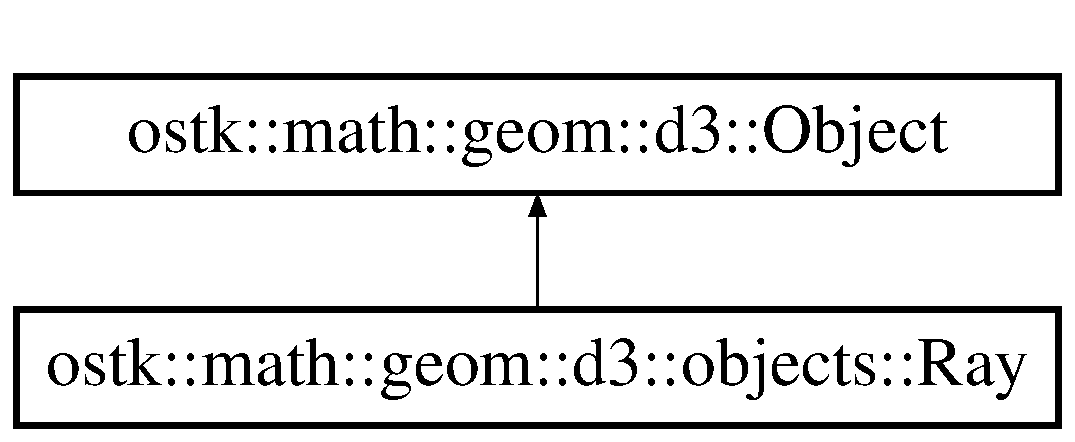
\includegraphics[height=2.000000cm]{classostk_1_1math_1_1geom_1_1d3_1_1objects_1_1_ray}
\end{center}
\end{figure}
\doxysubsection*{Public Member Functions}
\begin{DoxyCompactItemize}
\item 
\mbox{\hyperlink{classostk_1_1math_1_1geom_1_1d3_1_1objects_1_1_ray_a78335698f8a4f72e613e607b13121df0}{Ray}} (const \mbox{\hyperlink{classostk_1_1math_1_1geom_1_1d3_1_1objects_1_1_point}{Point}} \&an\+Origin, const Vector3d \&a\+Direction)
\begin{DoxyCompactList}\small\item\em Constructor. \end{DoxyCompactList}\item 
virtual \mbox{\hyperlink{classostk_1_1math_1_1geom_1_1d3_1_1objects_1_1_ray}{Ray}} $\ast$ \mbox{\hyperlink{classostk_1_1math_1_1geom_1_1d3_1_1objects_1_1_ray_aef341aa921aa184e1193c782e9198230}{clone}} () const override
\begin{DoxyCompactList}\small\item\em Clone ray. \end{DoxyCompactList}\item 
bool \mbox{\hyperlink{classostk_1_1math_1_1geom_1_1d3_1_1objects_1_1_ray_ad261573a0f3538dae39cd28c7d9a7dd2}{operator==}} (const \mbox{\hyperlink{classostk_1_1math_1_1geom_1_1d3_1_1objects_1_1_ray}{Ray}} \&a\+Ray) const
\begin{DoxyCompactList}\small\item\em Equal to operator. \end{DoxyCompactList}\item 
bool \mbox{\hyperlink{classostk_1_1math_1_1geom_1_1d3_1_1objects_1_1_ray_a9167ca5a0a3ad5a8c5e156231838aef3}{operator!=}} (const \mbox{\hyperlink{classostk_1_1math_1_1geom_1_1d3_1_1objects_1_1_ray}{Ray}} \&a\+Ray) const
\begin{DoxyCompactList}\small\item\em Not equal to operator. \end{DoxyCompactList}\item 
virtual bool \mbox{\hyperlink{classostk_1_1math_1_1geom_1_1d3_1_1objects_1_1_ray_ac0d991765b5d91a978fda87696b8069d}{is\+Defined}} () const override
\begin{DoxyCompactList}\small\item\em Check if ray is defined. \end{DoxyCompactList}\item 
bool \mbox{\hyperlink{classostk_1_1math_1_1geom_1_1d3_1_1objects_1_1_ray_aef14073eca198acde6dd1fe080939e42}{intersects}} (const \mbox{\hyperlink{classostk_1_1math_1_1geom_1_1d3_1_1objects_1_1_point}{Point}} \&a\+Point) const
\begin{DoxyCompactList}\small\item\em Check if ray intersects point. \end{DoxyCompactList}\item 
bool \mbox{\hyperlink{classostk_1_1math_1_1geom_1_1d3_1_1objects_1_1_ray_a8eb58fe0f0aaa491008112f411b49c33}{intersects}} (const \mbox{\hyperlink{classostk_1_1math_1_1geom_1_1d3_1_1objects_1_1_plane}{Plane}} \&a\+Plane) const
\begin{DoxyCompactList}\small\item\em Check if ray intersects plane. \end{DoxyCompactList}\item 
bool \mbox{\hyperlink{classostk_1_1math_1_1geom_1_1d3_1_1objects_1_1_ray_a0b01dbc44a2f8afdbef8495ab09d7457}{intersects}} (const \mbox{\hyperlink{classostk_1_1math_1_1geom_1_1d3_1_1objects_1_1_sphere}{Sphere}} \&a\+Sphere) const
\begin{DoxyCompactList}\small\item\em Check if ray intersects sphere. \end{DoxyCompactList}\item 
bool \mbox{\hyperlink{classostk_1_1math_1_1geom_1_1d3_1_1objects_1_1_ray_a48652010593cea440e028d9c02195108}{intersects}} (const \mbox{\hyperlink{classostk_1_1math_1_1geom_1_1d3_1_1objects_1_1_ellipsoid}{Ellipsoid}} \&an\+Ellipsoid) const
\begin{DoxyCompactList}\small\item\em Check if ray intersects ellipsoid. \end{DoxyCompactList}\item 
bool \mbox{\hyperlink{classostk_1_1math_1_1geom_1_1d3_1_1objects_1_1_ray_a7a8791f8658c741fd8ce967511ed2f5f}{contains}} (const \mbox{\hyperlink{classostk_1_1math_1_1geom_1_1d3_1_1objects_1_1_point}{Point}} \&a\+Point) const
\begin{DoxyCompactList}\small\item\em Check if ray contains point. \end{DoxyCompactList}\item 
bool \mbox{\hyperlink{classostk_1_1math_1_1geom_1_1d3_1_1objects_1_1_ray_a4433e066d6de57630140527bc74442ec}{contains}} (const \mbox{\hyperlink{classostk_1_1math_1_1geom_1_1d3_1_1objects_1_1_point_set}{Point\+Set}} \&a\+Point\+Set) const
\begin{DoxyCompactList}\small\item\em Check if ray contains point set. \end{DoxyCompactList}\item 
\mbox{\hyperlink{classostk_1_1math_1_1geom_1_1d3_1_1objects_1_1_point}{Point}} \mbox{\hyperlink{classostk_1_1math_1_1geom_1_1d3_1_1objects_1_1_ray_a8c47fac4d487986b538b8168484527c2}{get\+Origin}} () const
\begin{DoxyCompactList}\small\item\em Get ray origin. \end{DoxyCompactList}\item 
Vector3d \mbox{\hyperlink{classostk_1_1math_1_1geom_1_1d3_1_1objects_1_1_ray_a986aa3d13740b411f72115503b1c9a72}{get\+Direction}} () const
\begin{DoxyCompactList}\small\item\em Get ray direction. \end{DoxyCompactList}\item 
Real \mbox{\hyperlink{classostk_1_1math_1_1geom_1_1d3_1_1objects_1_1_ray_a9c7b98506891aac4fa9f3d20939fcf67}{distance\+To}} (const \mbox{\hyperlink{classostk_1_1math_1_1geom_1_1d3_1_1objects_1_1_point}{Point}} \&a\+Point) const
\begin{DoxyCompactList}\small\item\em Get distance to point. \end{DoxyCompactList}\item 
\mbox{\hyperlink{classostk_1_1math_1_1geom_1_1d3_1_1_intersection}{Intersection}} \mbox{\hyperlink{classostk_1_1math_1_1geom_1_1d3_1_1objects_1_1_ray_aa4625c2dfe200ab9df245d2a4dc92f64}{intersection\+With}} (const \mbox{\hyperlink{classostk_1_1math_1_1geom_1_1d3_1_1objects_1_1_plane}{Plane}} \&a\+Plane) const
\begin{DoxyCompactList}\small\item\em Compute intersection of ray with plane. \end{DoxyCompactList}\item 
\mbox{\hyperlink{classostk_1_1math_1_1geom_1_1d3_1_1_intersection}{Intersection}} \mbox{\hyperlink{classostk_1_1math_1_1geom_1_1d3_1_1objects_1_1_ray_ad51ec740a903fc78304898a08d28103b}{intersection\+With}} (const \mbox{\hyperlink{classostk_1_1math_1_1geom_1_1d3_1_1objects_1_1_sphere}{Sphere}} \&a\+Sphere, const bool only\+In\+Sight=\mbox{\hyperlink{_sphere_8hpp_af424617f7c785f4835e2feba5a5640f2}{D\+E\+F\+A\+U\+L\+T\+\_\+\+O\+N\+L\+Y\+\_\+\+I\+N\+\_\+\+S\+I\+G\+HT}}) const
\begin{DoxyCompactList}\small\item\em Compute intersection of ray with sphere. \end{DoxyCompactList}\item 
\mbox{\hyperlink{classostk_1_1math_1_1geom_1_1d3_1_1_intersection}{Intersection}} \mbox{\hyperlink{classostk_1_1math_1_1geom_1_1d3_1_1objects_1_1_ray_abc3d3b69f26e6a43e9b10b55e0fc8a45}{intersection\+With}} (const \mbox{\hyperlink{classostk_1_1math_1_1geom_1_1d3_1_1objects_1_1_ellipsoid}{Ellipsoid}} \&an\+Ellipsoid, const bool only\+In\+Sight=\mbox{\hyperlink{_sphere_8hpp_af424617f7c785f4835e2feba5a5640f2}{D\+E\+F\+A\+U\+L\+T\+\_\+\+O\+N\+L\+Y\+\_\+\+I\+N\+\_\+\+S\+I\+G\+HT}}) const
\begin{DoxyCompactList}\small\item\em Compute intersection of ray with ellipsoid. \end{DoxyCompactList}\item 
virtual void \mbox{\hyperlink{classostk_1_1math_1_1geom_1_1d3_1_1objects_1_1_ray_af2aed02d301de6d224cc757b7db573a7}{print}} (std\+::ostream \&an\+Output\+Stream, bool display\+Decorators=true) const override
\begin{DoxyCompactList}\small\item\em Print ray. \end{DoxyCompactList}\item 
virtual void \mbox{\hyperlink{classostk_1_1math_1_1geom_1_1d3_1_1objects_1_1_ray_abdbc52aa6745f9d9601a8138a519d828}{apply\+Transformation}} (const \mbox{\hyperlink{classostk_1_1math_1_1geom_1_1d3_1_1_transformation}{Transformation}} \&a\+Transformation) override
\begin{DoxyCompactList}\small\item\em Apply transformation to ray. \end{DoxyCompactList}\end{DoxyCompactItemize}
\doxysubsection*{Static Public Member Functions}
\begin{DoxyCompactItemize}
\item 
static \mbox{\hyperlink{classostk_1_1math_1_1geom_1_1d3_1_1objects_1_1_ray}{Ray}} \mbox{\hyperlink{classostk_1_1math_1_1geom_1_1d3_1_1objects_1_1_ray_a858510b6478f7cb47b763df6c641dfa7}{Undefined}} ()
\begin{DoxyCompactList}\small\item\em Constructs an undefined ray. \end{DoxyCompactList}\end{DoxyCompactItemize}


\doxysubsection{Detailed Description}
\mbox{\hyperlink{classostk_1_1math_1_1geom_1_1d3_1_1objects_1_1_ray}{Ray}}. 

\href{https://en.wikipedia.org/wiki/Line_}{\texttt{ https\+://en.\+wikipedia.\+org/wiki/\+Line\+\_\+}}(geometry)\mbox{\hyperlink{classostk_1_1math_1_1geom_1_1d3_1_1objects_1_1_ray_a78335698f8a4f72e613e607b13121df0}{Ray}} 

\doxysubsection{Constructor \& Destructor Documentation}
\mbox{\Hypertarget{classostk_1_1math_1_1geom_1_1d3_1_1objects_1_1_ray_a78335698f8a4f72e613e607b13121df0}\label{classostk_1_1math_1_1geom_1_1d3_1_1objects_1_1_ray_a78335698f8a4f72e613e607b13121df0}} 
\index{ostk::math::geom::d3::objects::Ray@{ostk::math::geom::d3::objects::Ray}!Ray@{Ray}}
\index{Ray@{Ray}!ostk::math::geom::d3::objects::Ray@{ostk::math::geom::d3::objects::Ray}}
\doxysubsubsection{\texorpdfstring{Ray()}{Ray()}}
{\footnotesize\ttfamily ostk\+::math\+::geom\+::d3\+::objects\+::\+Ray\+::\+Ray (\begin{DoxyParamCaption}\item[{const \mbox{\hyperlink{classostk_1_1math_1_1geom_1_1d3_1_1objects_1_1_point}{Point}} \&}]{an\+Origin,  }\item[{const Vector3d \&}]{a\+Direction }\end{DoxyParamCaption})}



Constructor. 


\begin{DoxyCode}{0}
\DoxyCodeLine{\mbox{\hyperlink{classostk_1_1math_1_1geom_1_1d3_1_1objects_1_1_ray_a78335698f8a4f72e613e607b13121df0}{Ray}} ray(\{ 0.0, 0.0, 0.0 \}, \{ 0.0, 0.0, 1.0 \}) ;}
\end{DoxyCode}



\begin{DoxyParams}[1]{Parameters}
\mbox{\texttt{ in}}  & {\em an\+Origin} & A ray origin \\
\hline
\mbox{\texttt{ in}}  & {\em a\+Direction} & A ray direction \\
\hline
\end{DoxyParams}


\doxysubsection{Member Function Documentation}
\mbox{\Hypertarget{classostk_1_1math_1_1geom_1_1d3_1_1objects_1_1_ray_abdbc52aa6745f9d9601a8138a519d828}\label{classostk_1_1math_1_1geom_1_1d3_1_1objects_1_1_ray_abdbc52aa6745f9d9601a8138a519d828}} 
\index{ostk::math::geom::d3::objects::Ray@{ostk::math::geom::d3::objects::Ray}!applyTransformation@{applyTransformation}}
\index{applyTransformation@{applyTransformation}!ostk::math::geom::d3::objects::Ray@{ostk::math::geom::d3::objects::Ray}}
\doxysubsubsection{\texorpdfstring{applyTransformation()}{applyTransformation()}}
{\footnotesize\ttfamily void ostk\+::math\+::geom\+::d3\+::objects\+::\+Ray\+::apply\+Transformation (\begin{DoxyParamCaption}\item[{const \mbox{\hyperlink{classostk_1_1math_1_1geom_1_1d3_1_1_transformation}{Transformation}} \&}]{a\+Transformation }\end{DoxyParamCaption})\hspace{0.3cm}{\ttfamily [override]}, {\ttfamily [virtual]}}



Apply transformation to ray. 


\begin{DoxyParams}[1]{Parameters}
\mbox{\texttt{ in}}  & {\em a\+Transformation} & A transformation \\
\hline
\end{DoxyParams}


Implements \mbox{\hyperlink{classostk_1_1math_1_1geom_1_1d3_1_1_object_ae9194dd6d2bb4df09292ffc84dccdb1d}{ostk\+::math\+::geom\+::d3\+::\+Object}}.

\mbox{\Hypertarget{classostk_1_1math_1_1geom_1_1d3_1_1objects_1_1_ray_aef341aa921aa184e1193c782e9198230}\label{classostk_1_1math_1_1geom_1_1d3_1_1objects_1_1_ray_aef341aa921aa184e1193c782e9198230}} 
\index{ostk::math::geom::d3::objects::Ray@{ostk::math::geom::d3::objects::Ray}!clone@{clone}}
\index{clone@{clone}!ostk::math::geom::d3::objects::Ray@{ostk::math::geom::d3::objects::Ray}}
\doxysubsubsection{\texorpdfstring{clone()}{clone()}}
{\footnotesize\ttfamily \mbox{\hyperlink{classostk_1_1math_1_1geom_1_1d3_1_1objects_1_1_ray}{Ray}} $\ast$ ostk\+::math\+::geom\+::d3\+::objects\+::\+Ray\+::clone (\begin{DoxyParamCaption}{ }\end{DoxyParamCaption}) const\hspace{0.3cm}{\ttfamily [override]}, {\ttfamily [virtual]}}



Clone ray. 

\begin{DoxyReturn}{Returns}
Pointer to cloned ray 
\end{DoxyReturn}


Implements \mbox{\hyperlink{classostk_1_1math_1_1geom_1_1d3_1_1_object_a676013f9555f6492687f9809b2db887b}{ostk\+::math\+::geom\+::d3\+::\+Object}}.

\mbox{\Hypertarget{classostk_1_1math_1_1geom_1_1d3_1_1objects_1_1_ray_a7a8791f8658c741fd8ce967511ed2f5f}\label{classostk_1_1math_1_1geom_1_1d3_1_1objects_1_1_ray_a7a8791f8658c741fd8ce967511ed2f5f}} 
\index{ostk::math::geom::d3::objects::Ray@{ostk::math::geom::d3::objects::Ray}!contains@{contains}}
\index{contains@{contains}!ostk::math::geom::d3::objects::Ray@{ostk::math::geom::d3::objects::Ray}}
\doxysubsubsection{\texorpdfstring{contains()}{contains()}\hspace{0.1cm}{\footnotesize\ttfamily [1/2]}}
{\footnotesize\ttfamily bool ostk\+::math\+::geom\+::d3\+::objects\+::\+Ray\+::contains (\begin{DoxyParamCaption}\item[{const \mbox{\hyperlink{classostk_1_1math_1_1geom_1_1d3_1_1objects_1_1_point}{Point}} \&}]{a\+Point }\end{DoxyParamCaption}) const}



Check if ray contains point. 


\begin{DoxyCode}{0}
\DoxyCodeLine{\mbox{\hyperlink{classostk_1_1math_1_1geom_1_1d3_1_1objects_1_1_ray_a78335698f8a4f72e613e607b13121df0}{Ray}} ray = ... ;}
\DoxyCodeLine{Point point = ... ;}
\DoxyCodeLine{ray.contains(point) ;}
\end{DoxyCode}



\begin{DoxyParams}[1]{Parameters}
\mbox{\texttt{ in}}  & {\em a\+Point} & A point \\
\hline
\end{DoxyParams}
\begin{DoxyReturn}{Returns}
True if ray contains point 
\end{DoxyReturn}
\mbox{\Hypertarget{classostk_1_1math_1_1geom_1_1d3_1_1objects_1_1_ray_a4433e066d6de57630140527bc74442ec}\label{classostk_1_1math_1_1geom_1_1d3_1_1objects_1_1_ray_a4433e066d6de57630140527bc74442ec}} 
\index{ostk::math::geom::d3::objects::Ray@{ostk::math::geom::d3::objects::Ray}!contains@{contains}}
\index{contains@{contains}!ostk::math::geom::d3::objects::Ray@{ostk::math::geom::d3::objects::Ray}}
\doxysubsubsection{\texorpdfstring{contains()}{contains()}\hspace{0.1cm}{\footnotesize\ttfamily [2/2]}}
{\footnotesize\ttfamily bool ostk\+::math\+::geom\+::d3\+::objects\+::\+Ray\+::contains (\begin{DoxyParamCaption}\item[{const \mbox{\hyperlink{classostk_1_1math_1_1geom_1_1d3_1_1objects_1_1_point_set}{Point\+Set}} \&}]{a\+Point\+Set }\end{DoxyParamCaption}) const}



Check if ray contains point set. 


\begin{DoxyCode}{0}
\DoxyCodeLine{\mbox{\hyperlink{classostk_1_1math_1_1geom_1_1d3_1_1objects_1_1_ray_a78335698f8a4f72e613e607b13121df0}{Ray}} ray = ... ;}
\DoxyCodeLine{PointSet pointSet = ... ;}
\DoxyCodeLine{ray.contains(pointSet) ;}
\end{DoxyCode}



\begin{DoxyParams}[1]{Parameters}
\mbox{\texttt{ in}}  & {\em a\+Point\+Set} & A point set \\
\hline
\end{DoxyParams}
\begin{DoxyReturn}{Returns}
True if ray contains point set 
\end{DoxyReturn}
\mbox{\Hypertarget{classostk_1_1math_1_1geom_1_1d3_1_1objects_1_1_ray_a9c7b98506891aac4fa9f3d20939fcf67}\label{classostk_1_1math_1_1geom_1_1d3_1_1objects_1_1_ray_a9c7b98506891aac4fa9f3d20939fcf67}} 
\index{ostk::math::geom::d3::objects::Ray@{ostk::math::geom::d3::objects::Ray}!distanceTo@{distanceTo}}
\index{distanceTo@{distanceTo}!ostk::math::geom::d3::objects::Ray@{ostk::math::geom::d3::objects::Ray}}
\doxysubsubsection{\texorpdfstring{distanceTo()}{distanceTo()}}
{\footnotesize\ttfamily Real ostk\+::math\+::geom\+::d3\+::objects\+::\+Ray\+::distance\+To (\begin{DoxyParamCaption}\item[{const \mbox{\hyperlink{classostk_1_1math_1_1geom_1_1d3_1_1objects_1_1_point}{Point}} \&}]{a\+Point }\end{DoxyParamCaption}) const}



Get distance to point. 


\begin{DoxyParams}[1]{Parameters}
\mbox{\texttt{ in}}  & {\em a\+Point} & A point \\
\hline
\end{DoxyParams}
\begin{DoxyReturn}{Returns}
Distance to point 
\end{DoxyReturn}
\mbox{\Hypertarget{classostk_1_1math_1_1geom_1_1d3_1_1objects_1_1_ray_a986aa3d13740b411f72115503b1c9a72}\label{classostk_1_1math_1_1geom_1_1d3_1_1objects_1_1_ray_a986aa3d13740b411f72115503b1c9a72}} 
\index{ostk::math::geom::d3::objects::Ray@{ostk::math::geom::d3::objects::Ray}!getDirection@{getDirection}}
\index{getDirection@{getDirection}!ostk::math::geom::d3::objects::Ray@{ostk::math::geom::d3::objects::Ray}}
\doxysubsubsection{\texorpdfstring{getDirection()}{getDirection()}}
{\footnotesize\ttfamily Vector3d ostk\+::math\+::geom\+::d3\+::objects\+::\+Ray\+::get\+Direction (\begin{DoxyParamCaption}{ }\end{DoxyParamCaption}) const}



Get ray direction. 


\begin{DoxyCode}{0}
\DoxyCodeLine{\mbox{\hyperlink{classostk_1_1math_1_1geom_1_1d3_1_1objects_1_1_ray_a78335698f8a4f72e613e607b13121df0}{Ray}}(\{ 0.0, 0.0, 0.0 \}, \{ 0.0, 0.0, 1.0 \}).\mbox{\hyperlink{classostk_1_1math_1_1geom_1_1d3_1_1objects_1_1_ray_a986aa3d13740b411f72115503b1c9a72}{getDirection}}() ; \textcolor{comment}{// [0.0, 0.0, 1.0]}}
\end{DoxyCode}


\begin{DoxyReturn}{Returns}
\mbox{\hyperlink{classostk_1_1math_1_1geom_1_1d3_1_1objects_1_1_ray}{Ray}} direction 
\end{DoxyReturn}
\mbox{\Hypertarget{classostk_1_1math_1_1geom_1_1d3_1_1objects_1_1_ray_a8c47fac4d487986b538b8168484527c2}\label{classostk_1_1math_1_1geom_1_1d3_1_1objects_1_1_ray_a8c47fac4d487986b538b8168484527c2}} 
\index{ostk::math::geom::d3::objects::Ray@{ostk::math::geom::d3::objects::Ray}!getOrigin@{getOrigin}}
\index{getOrigin@{getOrigin}!ostk::math::geom::d3::objects::Ray@{ostk::math::geom::d3::objects::Ray}}
\doxysubsubsection{\texorpdfstring{getOrigin()}{getOrigin()}}
{\footnotesize\ttfamily \mbox{\hyperlink{classostk_1_1math_1_1geom_1_1d3_1_1objects_1_1_point}{Point}} ostk\+::math\+::geom\+::d3\+::objects\+::\+Ray\+::get\+Origin (\begin{DoxyParamCaption}{ }\end{DoxyParamCaption}) const}



Get ray origin. 


\begin{DoxyCode}{0}
\DoxyCodeLine{\mbox{\hyperlink{classostk_1_1math_1_1geom_1_1d3_1_1objects_1_1_ray_a78335698f8a4f72e613e607b13121df0}{Ray}}(\{ 0.0, 0.0, 0.0 \}, \{ 0.0, 0.0, 1.0 \}).\mbox{\hyperlink{classostk_1_1math_1_1geom_1_1d3_1_1objects_1_1_ray_a8c47fac4d487986b538b8168484527c2}{getOrigin}}() ; \textcolor{comment}{// [0.0, 0.0, 0.0]}}
\end{DoxyCode}


\begin{DoxyReturn}{Returns}
\mbox{\hyperlink{classostk_1_1math_1_1geom_1_1d3_1_1objects_1_1_ray}{Ray}} origin 
\end{DoxyReturn}
\mbox{\Hypertarget{classostk_1_1math_1_1geom_1_1d3_1_1objects_1_1_ray_abc3d3b69f26e6a43e9b10b55e0fc8a45}\label{classostk_1_1math_1_1geom_1_1d3_1_1objects_1_1_ray_abc3d3b69f26e6a43e9b10b55e0fc8a45}} 
\index{ostk::math::geom::d3::objects::Ray@{ostk::math::geom::d3::objects::Ray}!intersectionWith@{intersectionWith}}
\index{intersectionWith@{intersectionWith}!ostk::math::geom::d3::objects::Ray@{ostk::math::geom::d3::objects::Ray}}
\doxysubsubsection{\texorpdfstring{intersectionWith()}{intersectionWith()}\hspace{0.1cm}{\footnotesize\ttfamily [1/3]}}
{\footnotesize\ttfamily \mbox{\hyperlink{classostk_1_1math_1_1geom_1_1d3_1_1_intersection}{Intersection}} ostk\+::math\+::geom\+::d3\+::objects\+::\+Ray\+::intersection\+With (\begin{DoxyParamCaption}\item[{const \mbox{\hyperlink{classostk_1_1math_1_1geom_1_1d3_1_1objects_1_1_ellipsoid}{Ellipsoid}} \&}]{an\+Ellipsoid,  }\item[{const bool}]{only\+In\+Sight = {\ttfamily \mbox{\hyperlink{_sphere_8hpp_af424617f7c785f4835e2feba5a5640f2}{D\+E\+F\+A\+U\+L\+T\+\_\+\+O\+N\+L\+Y\+\_\+\+I\+N\+\_\+\+S\+I\+G\+HT}}} }\end{DoxyParamCaption}) const}



Compute intersection of ray with ellipsoid. 


\begin{DoxyParams}[1]{Parameters}
\mbox{\texttt{ in}}  & {\em an\+Ellipsoid} & An ellipsoid \\
\hline
\mbox{\texttt{ in}}  & {\em only\+In\+Sight} & (optional) If true, only return intersection points that are in sight \\
\hline
\end{DoxyParams}
\begin{DoxyReturn}{Returns}
\mbox{\hyperlink{classostk_1_1math_1_1geom_1_1d3_1_1_intersection}{Intersection}} of ray with ellipsoid 
\end{DoxyReturn}
\mbox{\Hypertarget{classostk_1_1math_1_1geom_1_1d3_1_1objects_1_1_ray_aa4625c2dfe200ab9df245d2a4dc92f64}\label{classostk_1_1math_1_1geom_1_1d3_1_1objects_1_1_ray_aa4625c2dfe200ab9df245d2a4dc92f64}} 
\index{ostk::math::geom::d3::objects::Ray@{ostk::math::geom::d3::objects::Ray}!intersectionWith@{intersectionWith}}
\index{intersectionWith@{intersectionWith}!ostk::math::geom::d3::objects::Ray@{ostk::math::geom::d3::objects::Ray}}
\doxysubsubsection{\texorpdfstring{intersectionWith()}{intersectionWith()}\hspace{0.1cm}{\footnotesize\ttfamily [2/3]}}
{\footnotesize\ttfamily \mbox{\hyperlink{classostk_1_1math_1_1geom_1_1d3_1_1_intersection}{Intersection}} ostk\+::math\+::geom\+::d3\+::objects\+::\+Ray\+::intersection\+With (\begin{DoxyParamCaption}\item[{const \mbox{\hyperlink{classostk_1_1math_1_1geom_1_1d3_1_1objects_1_1_plane}{Plane}} \&}]{a\+Plane }\end{DoxyParamCaption}) const}



Compute intersection of ray with plane. 


\begin{DoxyParams}[1]{Parameters}
\mbox{\texttt{ in}}  & {\em a\+Plane} & A plane \\
\hline
\end{DoxyParams}
\begin{DoxyReturn}{Returns}
\mbox{\hyperlink{classostk_1_1math_1_1geom_1_1d3_1_1_intersection}{Intersection}} of ray with plane 
\end{DoxyReturn}
\mbox{\Hypertarget{classostk_1_1math_1_1geom_1_1d3_1_1objects_1_1_ray_ad51ec740a903fc78304898a08d28103b}\label{classostk_1_1math_1_1geom_1_1d3_1_1objects_1_1_ray_ad51ec740a903fc78304898a08d28103b}} 
\index{ostk::math::geom::d3::objects::Ray@{ostk::math::geom::d3::objects::Ray}!intersectionWith@{intersectionWith}}
\index{intersectionWith@{intersectionWith}!ostk::math::geom::d3::objects::Ray@{ostk::math::geom::d3::objects::Ray}}
\doxysubsubsection{\texorpdfstring{intersectionWith()}{intersectionWith()}\hspace{0.1cm}{\footnotesize\ttfamily [3/3]}}
{\footnotesize\ttfamily \mbox{\hyperlink{classostk_1_1math_1_1geom_1_1d3_1_1_intersection}{Intersection}} ostk\+::math\+::geom\+::d3\+::objects\+::\+Ray\+::intersection\+With (\begin{DoxyParamCaption}\item[{const \mbox{\hyperlink{classostk_1_1math_1_1geom_1_1d3_1_1objects_1_1_sphere}{Sphere}} \&}]{a\+Sphere,  }\item[{const bool}]{only\+In\+Sight = {\ttfamily \mbox{\hyperlink{_sphere_8hpp_af424617f7c785f4835e2feba5a5640f2}{D\+E\+F\+A\+U\+L\+T\+\_\+\+O\+N\+L\+Y\+\_\+\+I\+N\+\_\+\+S\+I\+G\+HT}}} }\end{DoxyParamCaption}) const}



Compute intersection of ray with sphere. 


\begin{DoxyParams}[1]{Parameters}
\mbox{\texttt{ in}}  & {\em a\+Sphere} & A sphere \\
\hline
\mbox{\texttt{ in}}  & {\em only\+In\+Sight} & (optional) If true, only return intersection points that are in sight \\
\hline
\end{DoxyParams}
\begin{DoxyReturn}{Returns}
\mbox{\hyperlink{classostk_1_1math_1_1geom_1_1d3_1_1_intersection}{Intersection}} of ray with sphere 
\end{DoxyReturn}
\mbox{\Hypertarget{classostk_1_1math_1_1geom_1_1d3_1_1objects_1_1_ray_a48652010593cea440e028d9c02195108}\label{classostk_1_1math_1_1geom_1_1d3_1_1objects_1_1_ray_a48652010593cea440e028d9c02195108}} 
\index{ostk::math::geom::d3::objects::Ray@{ostk::math::geom::d3::objects::Ray}!intersects@{intersects}}
\index{intersects@{intersects}!ostk::math::geom::d3::objects::Ray@{ostk::math::geom::d3::objects::Ray}}
\doxysubsubsection{\texorpdfstring{intersects()}{intersects()}\hspace{0.1cm}{\footnotesize\ttfamily [1/4]}}
{\footnotesize\ttfamily bool ostk\+::math\+::geom\+::d3\+::objects\+::\+Ray\+::intersects (\begin{DoxyParamCaption}\item[{const \mbox{\hyperlink{classostk_1_1math_1_1geom_1_1d3_1_1objects_1_1_ellipsoid}{Ellipsoid}} \&}]{an\+Ellipsoid }\end{DoxyParamCaption}) const}



Check if ray intersects ellipsoid. 


\begin{DoxyCode}{0}
\DoxyCodeLine{\mbox{\hyperlink{classostk_1_1math_1_1geom_1_1d3_1_1objects_1_1_ray_a78335698f8a4f72e613e607b13121df0}{Ray}} ray = ... ;}
\DoxyCodeLine{Ellipsoid ellipsoid = ... ;}
\DoxyCodeLine{ray.intersects(ellipsoid) ;}
\end{DoxyCode}



\begin{DoxyParams}[1]{Parameters}
\mbox{\texttt{ in}}  & {\em an\+Ellipsoid} & An ellipsoid \\
\hline
\end{DoxyParams}
\begin{DoxyReturn}{Returns}
True if ray intersects ellipsoid 
\end{DoxyReturn}
\mbox{\Hypertarget{classostk_1_1math_1_1geom_1_1d3_1_1objects_1_1_ray_a8eb58fe0f0aaa491008112f411b49c33}\label{classostk_1_1math_1_1geom_1_1d3_1_1objects_1_1_ray_a8eb58fe0f0aaa491008112f411b49c33}} 
\index{ostk::math::geom::d3::objects::Ray@{ostk::math::geom::d3::objects::Ray}!intersects@{intersects}}
\index{intersects@{intersects}!ostk::math::geom::d3::objects::Ray@{ostk::math::geom::d3::objects::Ray}}
\doxysubsubsection{\texorpdfstring{intersects()}{intersects()}\hspace{0.1cm}{\footnotesize\ttfamily [2/4]}}
{\footnotesize\ttfamily bool ostk\+::math\+::geom\+::d3\+::objects\+::\+Ray\+::intersects (\begin{DoxyParamCaption}\item[{const \mbox{\hyperlink{classostk_1_1math_1_1geom_1_1d3_1_1objects_1_1_plane}{Plane}} \&}]{a\+Plane }\end{DoxyParamCaption}) const}



Check if ray intersects plane. 


\begin{DoxyCode}{0}
\DoxyCodeLine{\mbox{\hyperlink{classostk_1_1math_1_1geom_1_1d3_1_1objects_1_1_ray_a78335698f8a4f72e613e607b13121df0}{Ray}} ray = ... ;}
\DoxyCodeLine{Plane plane = ... ;}
\DoxyCodeLine{ray.intersects(plane) ;}
\end{DoxyCode}



\begin{DoxyParams}[1]{Parameters}
\mbox{\texttt{ in}}  & {\em a\+Plane} & A plane \\
\hline
\end{DoxyParams}
\begin{DoxyReturn}{Returns}
True if ray intersects plane 
\end{DoxyReturn}
\mbox{\Hypertarget{classostk_1_1math_1_1geom_1_1d3_1_1objects_1_1_ray_aef14073eca198acde6dd1fe080939e42}\label{classostk_1_1math_1_1geom_1_1d3_1_1objects_1_1_ray_aef14073eca198acde6dd1fe080939e42}} 
\index{ostk::math::geom::d3::objects::Ray@{ostk::math::geom::d3::objects::Ray}!intersects@{intersects}}
\index{intersects@{intersects}!ostk::math::geom::d3::objects::Ray@{ostk::math::geom::d3::objects::Ray}}
\doxysubsubsection{\texorpdfstring{intersects()}{intersects()}\hspace{0.1cm}{\footnotesize\ttfamily [3/4]}}
{\footnotesize\ttfamily bool ostk\+::math\+::geom\+::d3\+::objects\+::\+Ray\+::intersects (\begin{DoxyParamCaption}\item[{const \mbox{\hyperlink{classostk_1_1math_1_1geom_1_1d3_1_1objects_1_1_point}{Point}} \&}]{a\+Point }\end{DoxyParamCaption}) const}



Check if ray intersects point. 


\begin{DoxyCode}{0}
\DoxyCodeLine{\mbox{\hyperlink{classostk_1_1math_1_1geom_1_1d3_1_1objects_1_1_ray_a78335698f8a4f72e613e607b13121df0}{Ray}} ray = ... ;}
\DoxyCodeLine{Point point = ... ;}
\DoxyCodeLine{ray.intersects(point) ;}
\end{DoxyCode}



\begin{DoxyParams}[1]{Parameters}
\mbox{\texttt{ in}}  & {\em an\+Point} & A point \\
\hline
\end{DoxyParams}
\begin{DoxyReturn}{Returns}
True if ray intersects point 
\end{DoxyReturn}
\mbox{\Hypertarget{classostk_1_1math_1_1geom_1_1d3_1_1objects_1_1_ray_a0b01dbc44a2f8afdbef8495ab09d7457}\label{classostk_1_1math_1_1geom_1_1d3_1_1objects_1_1_ray_a0b01dbc44a2f8afdbef8495ab09d7457}} 
\index{ostk::math::geom::d3::objects::Ray@{ostk::math::geom::d3::objects::Ray}!intersects@{intersects}}
\index{intersects@{intersects}!ostk::math::geom::d3::objects::Ray@{ostk::math::geom::d3::objects::Ray}}
\doxysubsubsection{\texorpdfstring{intersects()}{intersects()}\hspace{0.1cm}{\footnotesize\ttfamily [4/4]}}
{\footnotesize\ttfamily bool ostk\+::math\+::geom\+::d3\+::objects\+::\+Ray\+::intersects (\begin{DoxyParamCaption}\item[{const \mbox{\hyperlink{classostk_1_1math_1_1geom_1_1d3_1_1objects_1_1_sphere}{Sphere}} \&}]{a\+Sphere }\end{DoxyParamCaption}) const}



Check if ray intersects sphere. 


\begin{DoxyCode}{0}
\DoxyCodeLine{\mbox{\hyperlink{classostk_1_1math_1_1geom_1_1d3_1_1objects_1_1_ray_a78335698f8a4f72e613e607b13121df0}{Ray}} ray = ... ;}
\DoxyCodeLine{Sphere sphere = ... ;}
\DoxyCodeLine{ray.intersects(sphere) ;}
\end{DoxyCode}



\begin{DoxyParams}[1]{Parameters}
\mbox{\texttt{ in}}  & {\em an\+Sphere} & A sphere \\
\hline
\end{DoxyParams}
\begin{DoxyReturn}{Returns}
True if ray intersects sphere 
\end{DoxyReturn}
\mbox{\Hypertarget{classostk_1_1math_1_1geom_1_1d3_1_1objects_1_1_ray_ac0d991765b5d91a978fda87696b8069d}\label{classostk_1_1math_1_1geom_1_1d3_1_1objects_1_1_ray_ac0d991765b5d91a978fda87696b8069d}} 
\index{ostk::math::geom::d3::objects::Ray@{ostk::math::geom::d3::objects::Ray}!isDefined@{isDefined}}
\index{isDefined@{isDefined}!ostk::math::geom::d3::objects::Ray@{ostk::math::geom::d3::objects::Ray}}
\doxysubsubsection{\texorpdfstring{isDefined()}{isDefined()}}
{\footnotesize\ttfamily bool ostk\+::math\+::geom\+::d3\+::objects\+::\+Ray\+::is\+Defined (\begin{DoxyParamCaption}{ }\end{DoxyParamCaption}) const\hspace{0.3cm}{\ttfamily [override]}, {\ttfamily [virtual]}}



Check if ray is defined. 


\begin{DoxyCode}{0}
\DoxyCodeLine{\mbox{\hyperlink{classostk_1_1math_1_1geom_1_1d3_1_1objects_1_1_ray_a78335698f8a4f72e613e607b13121df0}{Ray}}(\{ 0.0, 0.0, 0.0 \}, \{ 0.0, 0.0, 1.0 \}).\mbox{\hyperlink{classostk_1_1math_1_1geom_1_1d3_1_1objects_1_1_ray_ac0d991765b5d91a978fda87696b8069d}{isDefined}}() ; \textcolor{comment}{// True}}
\end{DoxyCode}


\begin{DoxyReturn}{Returns}
True if ray is defined 
\end{DoxyReturn}


Implements \mbox{\hyperlink{classostk_1_1math_1_1geom_1_1d3_1_1_object_a271a1964cd208be85ce9a0a429395ad8}{ostk\+::math\+::geom\+::d3\+::\+Object}}.

\mbox{\Hypertarget{classostk_1_1math_1_1geom_1_1d3_1_1objects_1_1_ray_a9167ca5a0a3ad5a8c5e156231838aef3}\label{classostk_1_1math_1_1geom_1_1d3_1_1objects_1_1_ray_a9167ca5a0a3ad5a8c5e156231838aef3}} 
\index{ostk::math::geom::d3::objects::Ray@{ostk::math::geom::d3::objects::Ray}!operator"!=@{operator"!=}}
\index{operator"!=@{operator"!=}!ostk::math::geom::d3::objects::Ray@{ostk::math::geom::d3::objects::Ray}}
\doxysubsubsection{\texorpdfstring{operator"!=()}{operator!=()}}
{\footnotesize\ttfamily bool ostk\+::math\+::geom\+::d3\+::objects\+::\+Ray\+::operator!= (\begin{DoxyParamCaption}\item[{const \mbox{\hyperlink{classostk_1_1math_1_1geom_1_1d3_1_1objects_1_1_ray}{Ray}} \&}]{a\+Ray }\end{DoxyParamCaption}) const}



Not equal to operator. 


\begin{DoxyCode}{0}
\DoxyCodeLine{\mbox{\hyperlink{classostk_1_1math_1_1geom_1_1d3_1_1objects_1_1_ray_a78335698f8a4f72e613e607b13121df0}{Ray}}(\{ 0.0, 0.0, 0.0 \}, \{ 0.0, 0.0, 1.0 \}) != \mbox{\hyperlink{classostk_1_1math_1_1geom_1_1d3_1_1objects_1_1_ray_a78335698f8a4f72e613e607b13121df0}{Ray}}(\{ 0.0, 0.0, 0.0 \}, \{ 0.0, 0.0, 2.0 \}) ; \textcolor{comment}{//}}
\DoxyCodeLine{True}
\end{DoxyCode}



\begin{DoxyParams}[1]{Parameters}
\mbox{\texttt{ in}}  & {\em a\+Ray} & A ray \\
\hline
\end{DoxyParams}
\begin{DoxyReturn}{Returns}
True if rays are not equal 
\end{DoxyReturn}
\mbox{\Hypertarget{classostk_1_1math_1_1geom_1_1d3_1_1objects_1_1_ray_ad261573a0f3538dae39cd28c7d9a7dd2}\label{classostk_1_1math_1_1geom_1_1d3_1_1objects_1_1_ray_ad261573a0f3538dae39cd28c7d9a7dd2}} 
\index{ostk::math::geom::d3::objects::Ray@{ostk::math::geom::d3::objects::Ray}!operator==@{operator==}}
\index{operator==@{operator==}!ostk::math::geom::d3::objects::Ray@{ostk::math::geom::d3::objects::Ray}}
\doxysubsubsection{\texorpdfstring{operator==()}{operator==()}}
{\footnotesize\ttfamily bool ostk\+::math\+::geom\+::d3\+::objects\+::\+Ray\+::operator== (\begin{DoxyParamCaption}\item[{const \mbox{\hyperlink{classostk_1_1math_1_1geom_1_1d3_1_1objects_1_1_ray}{Ray}} \&}]{a\+Ray }\end{DoxyParamCaption}) const}



Equal to operator. 


\begin{DoxyCode}{0}
\DoxyCodeLine{\mbox{\hyperlink{classostk_1_1math_1_1geom_1_1d3_1_1objects_1_1_ray_a78335698f8a4f72e613e607b13121df0}{Ray}}(\{ 0.0, 0.0, 0.0 \}, \{ 0.0, 0.0, 1.0 \}) == \mbox{\hyperlink{classostk_1_1math_1_1geom_1_1d3_1_1objects_1_1_ray_a78335698f8a4f72e613e607b13121df0}{Ray}}(\{ 0.0, 0.0, 0.0 \}, \{ 0.0, 0.0, 1.0 \}) ; \textcolor{comment}{//}}
\DoxyCodeLine{True}
\end{DoxyCode}



\begin{DoxyParams}[1]{Parameters}
\mbox{\texttt{ in}}  & {\em a\+Ray} & A ray \\
\hline
\end{DoxyParams}
\begin{DoxyReturn}{Returns}
True if rays are equal 
\end{DoxyReturn}
\mbox{\Hypertarget{classostk_1_1math_1_1geom_1_1d3_1_1objects_1_1_ray_af2aed02d301de6d224cc757b7db573a7}\label{classostk_1_1math_1_1geom_1_1d3_1_1objects_1_1_ray_af2aed02d301de6d224cc757b7db573a7}} 
\index{ostk::math::geom::d3::objects::Ray@{ostk::math::geom::d3::objects::Ray}!print@{print}}
\index{print@{print}!ostk::math::geom::d3::objects::Ray@{ostk::math::geom::d3::objects::Ray}}
\doxysubsubsection{\texorpdfstring{print()}{print()}}
{\footnotesize\ttfamily void ostk\+::math\+::geom\+::d3\+::objects\+::\+Ray\+::print (\begin{DoxyParamCaption}\item[{std\+::ostream \&}]{an\+Output\+Stream,  }\item[{bool}]{display\+Decorators = {\ttfamily true} }\end{DoxyParamCaption}) const\hspace{0.3cm}{\ttfamily [override]}, {\ttfamily [virtual]}}



Print ray. 


\begin{DoxyParams}[1]{Parameters}
\mbox{\texttt{ in}}  & {\em an\+Output\+Stream} & An output stream \\
\hline
\mbox{\texttt{ in}}  & {\em (optional)} & display\+Decorators If true, display decorators \\
\hline
\end{DoxyParams}


Implements \mbox{\hyperlink{classostk_1_1math_1_1geom_1_1d3_1_1_object_ab2a2a782503b97d1cecabdfedc636fce}{ostk\+::math\+::geom\+::d3\+::\+Object}}.

\mbox{\Hypertarget{classostk_1_1math_1_1geom_1_1d3_1_1objects_1_1_ray_a858510b6478f7cb47b763df6c641dfa7}\label{classostk_1_1math_1_1geom_1_1d3_1_1objects_1_1_ray_a858510b6478f7cb47b763df6c641dfa7}} 
\index{ostk::math::geom::d3::objects::Ray@{ostk::math::geom::d3::objects::Ray}!Undefined@{Undefined}}
\index{Undefined@{Undefined}!ostk::math::geom::d3::objects::Ray@{ostk::math::geom::d3::objects::Ray}}
\doxysubsubsection{\texorpdfstring{Undefined()}{Undefined()}}
{\footnotesize\ttfamily \mbox{\hyperlink{classostk_1_1math_1_1geom_1_1d3_1_1objects_1_1_ray}{Ray}} ostk\+::math\+::geom\+::d3\+::objects\+::\+Ray\+::\+Undefined (\begin{DoxyParamCaption}{ }\end{DoxyParamCaption})\hspace{0.3cm}{\ttfamily [static]}}



Constructs an undefined ray. 


\begin{DoxyCode}{0}
\DoxyCodeLine{\mbox{\hyperlink{classostk_1_1math_1_1geom_1_1d3_1_1objects_1_1_ray_a78335698f8a4f72e613e607b13121df0}{Ray}} ray = \mbox{\hyperlink{classostk_1_1math_1_1geom_1_1d3_1_1objects_1_1_ray_a858510b6478f7cb47b763df6c641dfa7}{Ray::Undefined}}() ; \textcolor{comment}{// Undefined}}
\end{DoxyCode}


\begin{DoxyReturn}{Returns}
Undefined ray 
\end{DoxyReturn}


The documentation for this class was generated from the following files\+:\begin{DoxyCompactItemize}
\item 
include/\+Open\+Space\+Toolkit/\+Mathematics/\+Geometry/3\+D/\+Objects/\mbox{\hyperlink{_ray_8hpp}{Ray.\+hpp}}\item 
src/\+Open\+Space\+Toolkit/\+Mathematics/\+Geometry/3\+D/\+Objects/\mbox{\hyperlink{_ray_8cpp}{Ray.\+cpp}}\end{DoxyCompactItemize}

\hypertarget{classostk_1_1math_1_1geom_1_1d3_1_1trf_1_1rot_1_1_rotation_matrix}{}\doxysection{ostk\+::math\+::geom\+::d3\+::trf\+::rot\+::Rotation\+Matrix Class Reference}
\label{classostk_1_1math_1_1geom_1_1d3_1_1trf_1_1rot_1_1_rotation_matrix}\index{ostk::math::geom::d3::trf::rot::RotationMatrix@{ostk::math::geom::d3::trf::rot::RotationMatrix}}


Rotation matrix.  




{\ttfamily \#include $<$Rotation\+Matrix.\+hpp$>$}

\doxysubsection*{Public Member Functions}
\begin{DoxyCompactItemize}
\item 
\mbox{\hyperlink{classostk_1_1math_1_1geom_1_1d3_1_1trf_1_1rot_1_1_rotation_matrix_a5e6bed0779ad7db0c5bf26b2bd96f8ba}{Rotation\+Matrix}} (const Matrix3d \&a\+Matrix)
\begin{DoxyCompactList}\small\item\em Constructor. \end{DoxyCompactList}\item 
\mbox{\hyperlink{classostk_1_1math_1_1geom_1_1d3_1_1trf_1_1rot_1_1_rotation_matrix_ab82d268cc206957afae273a4fe5cc265}{Rotation\+Matrix}} (const Real \&a\+First\+Coefficient, const Real \&a\+Second\+Coefficient, const Real \&a\+Third\+Coefficient, const Real \&a\+Fourth\+Coefficient, const Real \&a\+Fifth\+Coefficient, const Real \&a\+Sixth\+Coefficient, const Real \&a\+Seventh\+Coefficient, const Real \&a\+Eighth\+Coefficient, const Real \&a\+Ninth\+Coefficient)
\begin{DoxyCompactList}\small\item\em Constructor. \end{DoxyCompactList}\item 
bool \mbox{\hyperlink{classostk_1_1math_1_1geom_1_1d3_1_1trf_1_1rot_1_1_rotation_matrix_a4563aa90935b926d8c1c7829ca333941}{operator==}} (const \mbox{\hyperlink{classostk_1_1math_1_1geom_1_1d3_1_1trf_1_1rot_1_1_rotation_matrix}{Rotation\+Matrix}} \&a\+Rotation\+Matrix) const
\begin{DoxyCompactList}\small\item\em Equal to operator. \end{DoxyCompactList}\item 
bool \mbox{\hyperlink{classostk_1_1math_1_1geom_1_1d3_1_1trf_1_1rot_1_1_rotation_matrix_a568d249ecc7071d8bb0d7a903221ee79}{operator!=}} (const \mbox{\hyperlink{classostk_1_1math_1_1geom_1_1d3_1_1trf_1_1rot_1_1_rotation_matrix}{Rotation\+Matrix}} \&a\+Rotation\+Matrix) const
\begin{DoxyCompactList}\small\item\em Not equal to operator. \end{DoxyCompactList}\item 
\mbox{\hyperlink{classostk_1_1math_1_1geom_1_1d3_1_1trf_1_1rot_1_1_rotation_matrix}{Rotation\+Matrix}} \mbox{\hyperlink{classostk_1_1math_1_1geom_1_1d3_1_1trf_1_1rot_1_1_rotation_matrix_a7b3316e6e63d7e82c64df4760be7ac9f}{operator$\ast$}} (const \mbox{\hyperlink{classostk_1_1math_1_1geom_1_1d3_1_1trf_1_1rot_1_1_rotation_matrix}{Rotation\+Matrix}} \&a\+Rotation\+Matrix) const
\begin{DoxyCompactList}\small\item\em Matrix multiplication operator. \end{DoxyCompactList}\item 
Vector3d \mbox{\hyperlink{classostk_1_1math_1_1geom_1_1d3_1_1trf_1_1rot_1_1_rotation_matrix_a465bbadfbf1b2dcd31f66250a8cdf02b}{operator$\ast$}} (const Vector3d \&a\+Vector) const
\begin{DoxyCompactList}\small\item\em Vector multiplication operator. \end{DoxyCompactList}\item 
double \mbox{\hyperlink{classostk_1_1math_1_1geom_1_1d3_1_1trf_1_1rot_1_1_rotation_matrix_a6b34e5000608d95cbd31ff3231fbc907}{operator()}} (const Index \&a\+Row\+Index, const Index \&a\+Column\+Index) const
\begin{DoxyCompactList}\small\item\em Index function operator. \end{DoxyCompactList}\item 
double \& \mbox{\hyperlink{classostk_1_1math_1_1geom_1_1d3_1_1trf_1_1rot_1_1_rotation_matrix_a87615eecad4bc8ed57d75c88ccafdbe6}{operator()}} (const Index \&a\+Row\+Index, const Index \&a\+Column\+Index)
\begin{DoxyCompactList}\small\item\em Index function operator. \end{DoxyCompactList}\item 
bool \mbox{\hyperlink{classostk_1_1math_1_1geom_1_1d3_1_1trf_1_1rot_1_1_rotation_matrix_a981ba00e3a2c145c1e6c80c2e5aef996}{is\+Defined}} () const
\begin{DoxyCompactList}\small\item\em Check if rotation matrix is defined. \end{DoxyCompactList}\item 
const Matrix3d \& \mbox{\hyperlink{classostk_1_1math_1_1geom_1_1d3_1_1trf_1_1rot_1_1_rotation_matrix_a31ae7b4eceeb4fc1deb10276cab54efa}{access\+Matrix}} () const
\begin{DoxyCompactList}\small\item\em Access underlying rotation matrix. \end{DoxyCompactList}\item 
Vector3d \mbox{\hyperlink{classostk_1_1math_1_1geom_1_1d3_1_1trf_1_1rot_1_1_rotation_matrix_a4dc63a231000b99be5338210835e3d5c}{get\+Row\+At}} (const Index \&a\+Row\+Index) const
\begin{DoxyCompactList}\small\item\em Get row at index. \end{DoxyCompactList}\item 
Vector3d \mbox{\hyperlink{classostk_1_1math_1_1geom_1_1d3_1_1trf_1_1rot_1_1_rotation_matrix_aef6eccb1b43b8759c55f14427cd4c4f0}{get\+Column\+At}} (const Index \&a\+Column\+Index) const
\begin{DoxyCompactList}\small\item\em Get column at index. \end{DoxyCompactList}\item 
Matrix3d \mbox{\hyperlink{classostk_1_1math_1_1geom_1_1d3_1_1trf_1_1rot_1_1_rotation_matrix_a23ca82706923577f771ca33b32298ee2}{get\+Matrix}} () const
\begin{DoxyCompactList}\small\item\em Get underlying rotation matrix. \end{DoxyCompactList}\item 
\mbox{\hyperlink{classostk_1_1math_1_1geom_1_1d3_1_1trf_1_1rot_1_1_rotation_matrix}{Rotation\+Matrix}} \mbox{\hyperlink{classostk_1_1math_1_1geom_1_1d3_1_1trf_1_1rot_1_1_rotation_matrix_a10bcc350ae896982a0939afe1234a86a}{to\+Transposed}} () const
\begin{DoxyCompactList}\small\item\em Get transposed rotation matrix. \end{DoxyCompactList}\item 
\mbox{\hyperlink{classostk_1_1math_1_1geom_1_1d3_1_1trf_1_1rot_1_1_rotation_matrix}{Rotation\+Matrix}} \& \mbox{\hyperlink{classostk_1_1math_1_1geom_1_1d3_1_1trf_1_1rot_1_1_rotation_matrix_aceb59983b55cc27128e0d720bcd4e1af}{transpose}} ()
\begin{DoxyCompactList}\small\item\em Transpose rotation matrix. \end{DoxyCompactList}\end{DoxyCompactItemize}
\doxysubsection*{Static Public Member Functions}
\begin{DoxyCompactItemize}
\item 
static \mbox{\hyperlink{classostk_1_1math_1_1geom_1_1d3_1_1trf_1_1rot_1_1_rotation_matrix}{Rotation\+Matrix}} \mbox{\hyperlink{classostk_1_1math_1_1geom_1_1d3_1_1trf_1_1rot_1_1_rotation_matrix_aa0d194dc4e0504fe29cf593b5b6182f4}{Undefined}} ()
\begin{DoxyCompactList}\small\item\em Constructs an undefined rotation matrix. \end{DoxyCompactList}\item 
static \mbox{\hyperlink{classostk_1_1math_1_1geom_1_1d3_1_1trf_1_1rot_1_1_rotation_matrix}{Rotation\+Matrix}} \mbox{\hyperlink{classostk_1_1math_1_1geom_1_1d3_1_1trf_1_1rot_1_1_rotation_matrix_a37c25a2ddaa1dcd24be8dd568259a9b8}{Unit}} ()
\begin{DoxyCompactList}\small\item\em Constructs a unit rotation matrix. \end{DoxyCompactList}\item 
static \mbox{\hyperlink{classostk_1_1math_1_1geom_1_1d3_1_1trf_1_1rot_1_1_rotation_matrix}{Rotation\+Matrix}} \mbox{\hyperlink{classostk_1_1math_1_1geom_1_1d3_1_1trf_1_1rot_1_1_rotation_matrix_a569b426de68866d30093a8fbe9958731}{RX}} (const \mbox{\hyperlink{classostk_1_1math_1_1geom_1_1_angle}{Angle}} \&a\+Rotation\+Angle)
\begin{DoxyCompactList}\small\item\em Constructs a rotation matrix representing a rotation around the X-\/axis. \end{DoxyCompactList}\item 
static \mbox{\hyperlink{classostk_1_1math_1_1geom_1_1d3_1_1trf_1_1rot_1_1_rotation_matrix}{Rotation\+Matrix}} \mbox{\hyperlink{classostk_1_1math_1_1geom_1_1d3_1_1trf_1_1rot_1_1_rotation_matrix_a4fceee0f8a617b37c34e1315ef877da8}{RY}} (const \mbox{\hyperlink{classostk_1_1math_1_1geom_1_1_angle}{Angle}} \&a\+Rotation\+Angle)
\begin{DoxyCompactList}\small\item\em Constructs a rotation matrix representing a rotation around the Y-\/axis. \end{DoxyCompactList}\item 
static \mbox{\hyperlink{classostk_1_1math_1_1geom_1_1d3_1_1trf_1_1rot_1_1_rotation_matrix}{Rotation\+Matrix}} \mbox{\hyperlink{classostk_1_1math_1_1geom_1_1d3_1_1trf_1_1rot_1_1_rotation_matrix_aef0a548981c37f3f7c8c53fec3f5e04e}{RZ}} (const \mbox{\hyperlink{classostk_1_1math_1_1geom_1_1_angle}{Angle}} \&a\+Rotation\+Angle)
\begin{DoxyCompactList}\small\item\em Constructs a rotation matrix representing a rotation around the Z-\/axis. \end{DoxyCompactList}\item 
static \mbox{\hyperlink{classostk_1_1math_1_1geom_1_1d3_1_1trf_1_1rot_1_1_rotation_matrix}{Rotation\+Matrix}} \mbox{\hyperlink{classostk_1_1math_1_1geom_1_1d3_1_1trf_1_1rot_1_1_rotation_matrix_a8316daca4e78cea8abb67611d73ac52a}{Rows}} (const Vector3d \&a\+First\+Row, const Vector3d \&a\+Second\+Row, const Vector3d \&a\+Third\+Row)
\begin{DoxyCompactList}\small\item\em Constructs a rotation matrix from row vectors. \end{DoxyCompactList}\item 
static \mbox{\hyperlink{classostk_1_1math_1_1geom_1_1d3_1_1trf_1_1rot_1_1_rotation_matrix}{Rotation\+Matrix}} \mbox{\hyperlink{classostk_1_1math_1_1geom_1_1d3_1_1trf_1_1rot_1_1_rotation_matrix_a244f95ea8a4298e92a9d927f9b8caa72}{Columns}} (const Vector3d \&a\+First\+Column, const Vector3d \&a\+Second\+Column, const Vector3d \&a\+Third\+Column)
\begin{DoxyCompactList}\small\item\em Constructs a rotation matrix from column vectors. \end{DoxyCompactList}\item 
static \mbox{\hyperlink{classostk_1_1math_1_1geom_1_1d3_1_1trf_1_1rot_1_1_rotation_matrix}{Rotation\+Matrix}} \mbox{\hyperlink{classostk_1_1math_1_1geom_1_1d3_1_1trf_1_1rot_1_1_rotation_matrix_ac327eae5f7a354639d05b6bdffdae640}{Quaternion}} (const \mbox{\hyperlink{classostk_1_1math_1_1geom_1_1d3_1_1trf_1_1rot_1_1_quaternion}{rot\+::\+Quaternion}} \&a\+Quaternion)
\begin{DoxyCompactList}\small\item\em Constructs a rotation matrix from a quaternion. \end{DoxyCompactList}\item 
static \mbox{\hyperlink{classostk_1_1math_1_1geom_1_1d3_1_1trf_1_1rot_1_1_rotation_matrix}{Rotation\+Matrix}} \mbox{\hyperlink{classostk_1_1math_1_1geom_1_1d3_1_1trf_1_1rot_1_1_rotation_matrix_a609da1b600078c74a84bcac864aa877b}{Rotation\+Vector}} (const \mbox{\hyperlink{classostk_1_1math_1_1geom_1_1d3_1_1trf_1_1rot_1_1_rotation_vector}{rot\+::\+Rotation\+Vector}} \&a\+Rotation\+Vector)
\begin{DoxyCompactList}\small\item\em Constructs a rotation matrix from a rotation vector. \end{DoxyCompactList}\end{DoxyCompactItemize}
\doxysubsection*{Friends}
\begin{DoxyCompactItemize}
\item 
std\+::ostream \& \mbox{\hyperlink{classostk_1_1math_1_1geom_1_1d3_1_1trf_1_1rot_1_1_rotation_matrix_aa9ed0897a6219331deeb7750017a0df9}{operator$<$$<$}} (std\+::ostream \&an\+Output\+Stream, const \mbox{\hyperlink{classostk_1_1math_1_1geom_1_1d3_1_1trf_1_1rot_1_1_rotation_matrix}{Rotation\+Matrix}} \&a\+Rotation\+Matrix)
\begin{DoxyCompactList}\small\item\em Output stream operator. \end{DoxyCompactList}\end{DoxyCompactItemize}


\doxysubsection{Detailed Description}
Rotation matrix. 

\href{https://en.wikipedia.org/wiki/Rotation_matrix}{\texttt{ https\+://en.\+wikipedia.\+org/wiki/\+Rotation\+\_\+matrix}} 

\doxysubsection{Constructor \& Destructor Documentation}
\mbox{\Hypertarget{classostk_1_1math_1_1geom_1_1d3_1_1trf_1_1rot_1_1_rotation_matrix_a5e6bed0779ad7db0c5bf26b2bd96f8ba}\label{classostk_1_1math_1_1geom_1_1d3_1_1trf_1_1rot_1_1_rotation_matrix_a5e6bed0779ad7db0c5bf26b2bd96f8ba}} 
\index{ostk::math::geom::d3::trf::rot::RotationMatrix@{ostk::math::geom::d3::trf::rot::RotationMatrix}!RotationMatrix@{RotationMatrix}}
\index{RotationMatrix@{RotationMatrix}!ostk::math::geom::d3::trf::rot::RotationMatrix@{ostk::math::geom::d3::trf::rot::RotationMatrix}}
\doxysubsubsection{\texorpdfstring{RotationMatrix()}{RotationMatrix()}\hspace{0.1cm}{\footnotesize\ttfamily [1/2]}}
{\footnotesize\ttfamily ostk\+::math\+::geom\+::d3\+::trf\+::rot\+::\+Rotation\+Matrix\+::\+Rotation\+Matrix (\begin{DoxyParamCaption}\item[{const Matrix3d \&}]{a\+Matrix }\end{DoxyParamCaption})}



Constructor. 


\begin{DoxyParams}[1]{Parameters}
\mbox{\texttt{ in}}  & {\em a\+Matrix} & A matrix \\
\hline
\end{DoxyParams}
\mbox{\Hypertarget{classostk_1_1math_1_1geom_1_1d3_1_1trf_1_1rot_1_1_rotation_matrix_ab82d268cc206957afae273a4fe5cc265}\label{classostk_1_1math_1_1geom_1_1d3_1_1trf_1_1rot_1_1_rotation_matrix_ab82d268cc206957afae273a4fe5cc265}} 
\index{ostk::math::geom::d3::trf::rot::RotationMatrix@{ostk::math::geom::d3::trf::rot::RotationMatrix}!RotationMatrix@{RotationMatrix}}
\index{RotationMatrix@{RotationMatrix}!ostk::math::geom::d3::trf::rot::RotationMatrix@{ostk::math::geom::d3::trf::rot::RotationMatrix}}
\doxysubsubsection{\texorpdfstring{RotationMatrix()}{RotationMatrix()}\hspace{0.1cm}{\footnotesize\ttfamily [2/2]}}
{\footnotesize\ttfamily ostk\+::math\+::geom\+::d3\+::trf\+::rot\+::\+Rotation\+Matrix\+::\+Rotation\+Matrix (\begin{DoxyParamCaption}\item[{const Real \&}]{a\+First\+Coefficient,  }\item[{const Real \&}]{a\+Second\+Coefficient,  }\item[{const Real \&}]{a\+Third\+Coefficient,  }\item[{const Real \&}]{a\+Fourth\+Coefficient,  }\item[{const Real \&}]{a\+Fifth\+Coefficient,  }\item[{const Real \&}]{a\+Sixth\+Coefficient,  }\item[{const Real \&}]{a\+Seventh\+Coefficient,  }\item[{const Real \&}]{a\+Eighth\+Coefficient,  }\item[{const Real \&}]{a\+Ninth\+Coefficient }\end{DoxyParamCaption})}



Constructor. 


\begin{DoxyParams}[1]{Parameters}
\mbox{\texttt{ in}}  & {\em a\+First\+Coefficient} & A first coefficient \\
\hline
\mbox{\texttt{ in}}  & {\em a\+Second\+Coefficient} & A second coefficient \\
\hline
\mbox{\texttt{ in}}  & {\em a\+Third\+Coefficient} & A third coefficient \\
\hline
\mbox{\texttt{ in}}  & {\em a\+Fourth\+Coefficient} & A fourth coefficient \\
\hline
\mbox{\texttt{ in}}  & {\em a\+Fifth\+Coefficient} & A fifth coefficient \\
\hline
\mbox{\texttt{ in}}  & {\em a\+Sixth\+Coefficient} & A sixth coefficient \\
\hline
\mbox{\texttt{ in}}  & {\em a\+Seventh\+Coefficient} & A seventh coefficient \\
\hline
\mbox{\texttt{ in}}  & {\em a\+Eighth\+Coefficient} & A eighth coefficient \\
\hline
\mbox{\texttt{ in}}  & {\em a\+Ninth\+Coefficient} & A ninth coefficient \\
\hline
\end{DoxyParams}


\doxysubsection{Member Function Documentation}
\mbox{\Hypertarget{classostk_1_1math_1_1geom_1_1d3_1_1trf_1_1rot_1_1_rotation_matrix_a31ae7b4eceeb4fc1deb10276cab54efa}\label{classostk_1_1math_1_1geom_1_1d3_1_1trf_1_1rot_1_1_rotation_matrix_a31ae7b4eceeb4fc1deb10276cab54efa}} 
\index{ostk::math::geom::d3::trf::rot::RotationMatrix@{ostk::math::geom::d3::trf::rot::RotationMatrix}!accessMatrix@{accessMatrix}}
\index{accessMatrix@{accessMatrix}!ostk::math::geom::d3::trf::rot::RotationMatrix@{ostk::math::geom::d3::trf::rot::RotationMatrix}}
\doxysubsubsection{\texorpdfstring{accessMatrix()}{accessMatrix()}}
{\footnotesize\ttfamily const Matrix3d \& ostk\+::math\+::geom\+::d3\+::trf\+::rot\+::\+Rotation\+Matrix\+::access\+Matrix (\begin{DoxyParamCaption}{ }\end{DoxyParamCaption}) const}



Access underlying rotation matrix. 

\begin{DoxyReturn}{Returns}
Reference to underlying rotation matrix 
\end{DoxyReturn}
\mbox{\Hypertarget{classostk_1_1math_1_1geom_1_1d3_1_1trf_1_1rot_1_1_rotation_matrix_a244f95ea8a4298e92a9d927f9b8caa72}\label{classostk_1_1math_1_1geom_1_1d3_1_1trf_1_1rot_1_1_rotation_matrix_a244f95ea8a4298e92a9d927f9b8caa72}} 
\index{ostk::math::geom::d3::trf::rot::RotationMatrix@{ostk::math::geom::d3::trf::rot::RotationMatrix}!Columns@{Columns}}
\index{Columns@{Columns}!ostk::math::geom::d3::trf::rot::RotationMatrix@{ostk::math::geom::d3::trf::rot::RotationMatrix}}
\doxysubsubsection{\texorpdfstring{Columns()}{Columns()}}
{\footnotesize\ttfamily \mbox{\hyperlink{classostk_1_1math_1_1geom_1_1d3_1_1trf_1_1rot_1_1_rotation_matrix}{Rotation\+Matrix}} ostk\+::math\+::geom\+::d3\+::trf\+::rot\+::\+Rotation\+Matrix\+::\+Columns (\begin{DoxyParamCaption}\item[{const Vector3d \&}]{a\+First\+Column,  }\item[{const Vector3d \&}]{a\+Second\+Column,  }\item[{const Vector3d \&}]{a\+Third\+Column }\end{DoxyParamCaption})\hspace{0.3cm}{\ttfamily [static]}}



Constructs a rotation matrix from column vectors. 


\begin{DoxyCode}{0}
\DoxyCodeLine{\mbox{\hyperlink{classostk_1_1math_1_1geom_1_1d3_1_1trf_1_1rot_1_1_rotation_matrix_a5e6bed0779ad7db0c5bf26b2bd96f8ba}{RotationMatrix}} rotationMatrix = \mbox{\hyperlink{classostk_1_1math_1_1geom_1_1d3_1_1trf_1_1rot_1_1_rotation_matrix_a244f95ea8a4298e92a9d927f9b8caa72}{RotationMatrix::Columns}}(\mbox{\hyperlink{namespaceostk_1_1math_1_1obj_a18744cbf433bce59f6758d9fe3b1dff1}{Vector3d}}(1.0, 0.0, 0.0),}
\DoxyCodeLine{\mbox{\hyperlink{namespaceostk_1_1math_1_1obj_a18744cbf433bce59f6758d9fe3b1dff1}{Vector3d}}(1.0, 0.0, 0.0), \mbox{\hyperlink{namespaceostk_1_1math_1_1obj_a18744cbf433bce59f6758d9fe3b1dff1}{Vector3d}}(1.0, 0.0, 0.0)) ;}
\end{DoxyCode}



\begin{DoxyParams}[1]{Parameters}
\mbox{\texttt{ in}}  & {\em a\+First\+Column} & A first column \\
\hline
\mbox{\texttt{ in}}  & {\em a\+Second\+Column} & A second column \\
\hline
\mbox{\texttt{ in}}  & {\em a\+Third\+Column} & A third column \\
\hline
\end{DoxyParams}
\begin{DoxyReturn}{Returns}
Rotation matrix 
\end{DoxyReturn}
\mbox{\Hypertarget{classostk_1_1math_1_1geom_1_1d3_1_1trf_1_1rot_1_1_rotation_matrix_aef6eccb1b43b8759c55f14427cd4c4f0}\label{classostk_1_1math_1_1geom_1_1d3_1_1trf_1_1rot_1_1_rotation_matrix_aef6eccb1b43b8759c55f14427cd4c4f0}} 
\index{ostk::math::geom::d3::trf::rot::RotationMatrix@{ostk::math::geom::d3::trf::rot::RotationMatrix}!getColumnAt@{getColumnAt}}
\index{getColumnAt@{getColumnAt}!ostk::math::geom::d3::trf::rot::RotationMatrix@{ostk::math::geom::d3::trf::rot::RotationMatrix}}
\doxysubsubsection{\texorpdfstring{getColumnAt()}{getColumnAt()}}
{\footnotesize\ttfamily Vector3d ostk\+::math\+::geom\+::d3\+::trf\+::rot\+::\+Rotation\+Matrix\+::get\+Column\+At (\begin{DoxyParamCaption}\item[{const Index \&}]{a\+Column\+Index }\end{DoxyParamCaption}) const}



Get column at index. 


\begin{DoxyParams}[1]{Parameters}
\mbox{\texttt{ in}}  & {\em a\+Column\+Index} & Index of column \\
\hline
\end{DoxyParams}
\begin{DoxyReturn}{Returns}
Column at index 
\end{DoxyReturn}
\mbox{\Hypertarget{classostk_1_1math_1_1geom_1_1d3_1_1trf_1_1rot_1_1_rotation_matrix_a23ca82706923577f771ca33b32298ee2}\label{classostk_1_1math_1_1geom_1_1d3_1_1trf_1_1rot_1_1_rotation_matrix_a23ca82706923577f771ca33b32298ee2}} 
\index{ostk::math::geom::d3::trf::rot::RotationMatrix@{ostk::math::geom::d3::trf::rot::RotationMatrix}!getMatrix@{getMatrix}}
\index{getMatrix@{getMatrix}!ostk::math::geom::d3::trf::rot::RotationMatrix@{ostk::math::geom::d3::trf::rot::RotationMatrix}}
\doxysubsubsection{\texorpdfstring{getMatrix()}{getMatrix()}}
{\footnotesize\ttfamily Matrix3d ostk\+::math\+::geom\+::d3\+::trf\+::rot\+::\+Rotation\+Matrix\+::get\+Matrix (\begin{DoxyParamCaption}{ }\end{DoxyParamCaption}) const}



Get underlying rotation matrix. 

\begin{DoxyReturn}{Returns}
Underlying rotation matrix 
\end{DoxyReturn}
\mbox{\Hypertarget{classostk_1_1math_1_1geom_1_1d3_1_1trf_1_1rot_1_1_rotation_matrix_a4dc63a231000b99be5338210835e3d5c}\label{classostk_1_1math_1_1geom_1_1d3_1_1trf_1_1rot_1_1_rotation_matrix_a4dc63a231000b99be5338210835e3d5c}} 
\index{ostk::math::geom::d3::trf::rot::RotationMatrix@{ostk::math::geom::d3::trf::rot::RotationMatrix}!getRowAt@{getRowAt}}
\index{getRowAt@{getRowAt}!ostk::math::geom::d3::trf::rot::RotationMatrix@{ostk::math::geom::d3::trf::rot::RotationMatrix}}
\doxysubsubsection{\texorpdfstring{getRowAt()}{getRowAt()}}
{\footnotesize\ttfamily Vector3d ostk\+::math\+::geom\+::d3\+::trf\+::rot\+::\+Rotation\+Matrix\+::get\+Row\+At (\begin{DoxyParamCaption}\item[{const Index \&}]{a\+Row\+Index }\end{DoxyParamCaption}) const}



Get row at index. 


\begin{DoxyParams}[1]{Parameters}
\mbox{\texttt{ in}}  & {\em a\+Row\+Index} & Index of row \\
\hline
\end{DoxyParams}
\begin{DoxyReturn}{Returns}
Row at index 
\end{DoxyReturn}
\mbox{\Hypertarget{classostk_1_1math_1_1geom_1_1d3_1_1trf_1_1rot_1_1_rotation_matrix_a981ba00e3a2c145c1e6c80c2e5aef996}\label{classostk_1_1math_1_1geom_1_1d3_1_1trf_1_1rot_1_1_rotation_matrix_a981ba00e3a2c145c1e6c80c2e5aef996}} 
\index{ostk::math::geom::d3::trf::rot::RotationMatrix@{ostk::math::geom::d3::trf::rot::RotationMatrix}!isDefined@{isDefined}}
\index{isDefined@{isDefined}!ostk::math::geom::d3::trf::rot::RotationMatrix@{ostk::math::geom::d3::trf::rot::RotationMatrix}}
\doxysubsubsection{\texorpdfstring{isDefined()}{isDefined()}}
{\footnotesize\ttfamily bool ostk\+::math\+::geom\+::d3\+::trf\+::rot\+::\+Rotation\+Matrix\+::is\+Defined (\begin{DoxyParamCaption}{ }\end{DoxyParamCaption}) const}



Check if rotation matrix is defined. 


\begin{DoxyCode}{0}
\DoxyCodeLine{\mbox{\hyperlink{classostk_1_1math_1_1geom_1_1d3_1_1trf_1_1rot_1_1_rotation_matrix_a5e6bed0779ad7db0c5bf26b2bd96f8ba}{RotationMatrix}}(\mbox{\hyperlink{namespaceostk_1_1math_1_1obj_a18744cbf433bce59f6758d9fe3b1dff1}{Vector3d}}(0.0, 0.0, 1.0), \mbox{\hyperlink{classostk_1_1math_1_1geom_1_1_angle_a2cefda601167af07f61f0477776203ca}{Angle::Degrees}}(90.0)).isDefined() ; \textcolor{comment}{// True}}
\end{DoxyCode}


\begin{DoxyReturn}{Returns}
True if rotation matrix is defined 
\end{DoxyReturn}
\mbox{\Hypertarget{classostk_1_1math_1_1geom_1_1d3_1_1trf_1_1rot_1_1_rotation_matrix_a568d249ecc7071d8bb0d7a903221ee79}\label{classostk_1_1math_1_1geom_1_1d3_1_1trf_1_1rot_1_1_rotation_matrix_a568d249ecc7071d8bb0d7a903221ee79}} 
\index{ostk::math::geom::d3::trf::rot::RotationMatrix@{ostk::math::geom::d3::trf::rot::RotationMatrix}!operator"!=@{operator"!=}}
\index{operator"!=@{operator"!=}!ostk::math::geom::d3::trf::rot::RotationMatrix@{ostk::math::geom::d3::trf::rot::RotationMatrix}}
\doxysubsubsection{\texorpdfstring{operator"!=()}{operator!=()}}
{\footnotesize\ttfamily bool ostk\+::math\+::geom\+::d3\+::trf\+::rot\+::\+Rotation\+Matrix\+::operator!= (\begin{DoxyParamCaption}\item[{const \mbox{\hyperlink{classostk_1_1math_1_1geom_1_1d3_1_1trf_1_1rot_1_1_rotation_matrix}{Rotation\+Matrix}} \&}]{a\+Rotation\+Matrix }\end{DoxyParamCaption}) const}



Not equal to operator. 


\begin{DoxyCode}{0}
\DoxyCodeLine{\mbox{\hyperlink{classostk_1_1math_1_1geom_1_1d3_1_1trf_1_1rot_1_1_rotation_matrix_a5e6bed0779ad7db0c5bf26b2bd96f8ba}{RotationMatrix}}(...) != \mbox{\hyperlink{classostk_1_1math_1_1geom_1_1d3_1_1trf_1_1rot_1_1_rotation_matrix_a5e6bed0779ad7db0c5bf26b2bd96f8ba}{RotationMatrix}}(...) ;}
\end{DoxyCode}



\begin{DoxyParams}[1]{Parameters}
\mbox{\texttt{ in}}  & {\em a\+Rotation\+Matrix} & A rotation matrix \\
\hline
\end{DoxyParams}
\begin{DoxyReturn}{Returns}
True if rotation matrices are not equal 
\end{DoxyReturn}
\mbox{\Hypertarget{classostk_1_1math_1_1geom_1_1d3_1_1trf_1_1rot_1_1_rotation_matrix_a87615eecad4bc8ed57d75c88ccafdbe6}\label{classostk_1_1math_1_1geom_1_1d3_1_1trf_1_1rot_1_1_rotation_matrix_a87615eecad4bc8ed57d75c88ccafdbe6}} 
\index{ostk::math::geom::d3::trf::rot::RotationMatrix@{ostk::math::geom::d3::trf::rot::RotationMatrix}!operator()@{operator()}}
\index{operator()@{operator()}!ostk::math::geom::d3::trf::rot::RotationMatrix@{ostk::math::geom::d3::trf::rot::RotationMatrix}}
\doxysubsubsection{\texorpdfstring{operator()()}{operator()()}\hspace{0.1cm}{\footnotesize\ttfamily [1/2]}}
{\footnotesize\ttfamily double \& ostk\+::math\+::geom\+::d3\+::trf\+::rot\+::\+Rotation\+Matrix\+::operator() (\begin{DoxyParamCaption}\item[{const Index \&}]{a\+Row\+Index,  }\item[{const Index \&}]{a\+Column\+Index }\end{DoxyParamCaption})}



Index function operator. 


\begin{DoxyCode}{0}
\DoxyCodeLine{\mbox{\hyperlink{classostk_1_1math_1_1geom_1_1d3_1_1trf_1_1rot_1_1_rotation_matrix_a5e6bed0779ad7db0c5bf26b2bd96f8ba}{RotationMatrix}} rotationMatrix = \mbox{\hyperlink{classostk_1_1math_1_1geom_1_1d3_1_1trf_1_1rot_1_1_rotation_matrix_a37c25a2ddaa1dcd24be8dd568259a9b8}{RotationMatrix::Unit}}() ;}
\DoxyCodeLine{rotationMatrix(0, 0) = 0.0 ;}
\end{DoxyCode}



\begin{DoxyParams}[1]{Parameters}
\mbox{\texttt{ in}}  & {\em a\+Row\+Index} & A row index \\
\hline
\mbox{\texttt{ in}}  & {\em a\+Column\+Index} & A column index \\
\hline
\end{DoxyParams}
\begin{DoxyReturn}{Returns}
Reference of value at index 
\end{DoxyReturn}
\mbox{\Hypertarget{classostk_1_1math_1_1geom_1_1d3_1_1trf_1_1rot_1_1_rotation_matrix_a6b34e5000608d95cbd31ff3231fbc907}\label{classostk_1_1math_1_1geom_1_1d3_1_1trf_1_1rot_1_1_rotation_matrix_a6b34e5000608d95cbd31ff3231fbc907}} 
\index{ostk::math::geom::d3::trf::rot::RotationMatrix@{ostk::math::geom::d3::trf::rot::RotationMatrix}!operator()@{operator()}}
\index{operator()@{operator()}!ostk::math::geom::d3::trf::rot::RotationMatrix@{ostk::math::geom::d3::trf::rot::RotationMatrix}}
\doxysubsubsection{\texorpdfstring{operator()()}{operator()()}\hspace{0.1cm}{\footnotesize\ttfamily [2/2]}}
{\footnotesize\ttfamily double ostk\+::math\+::geom\+::d3\+::trf\+::rot\+::\+Rotation\+Matrix\+::operator() (\begin{DoxyParamCaption}\item[{const Index \&}]{a\+Row\+Index,  }\item[{const Index \&}]{a\+Column\+Index }\end{DoxyParamCaption}) const}



Index function operator. 


\begin{DoxyCode}{0}
\DoxyCodeLine{\mbox{\hyperlink{classostk_1_1math_1_1geom_1_1d3_1_1trf_1_1rot_1_1_rotation_matrix_a5e6bed0779ad7db0c5bf26b2bd96f8ba}{RotationMatrix}} rotationMatrix = \mbox{\hyperlink{classostk_1_1math_1_1geom_1_1d3_1_1trf_1_1rot_1_1_rotation_matrix_a37c25a2ddaa1dcd24be8dd568259a9b8}{RotationMatrix::Unit}}() ;}
\DoxyCodeLine{\textcolor{keywordtype}{double} value\_00 = rotationMatrix(0, 0) ; \textcolor{comment}{// 1.0}}
\end{DoxyCode}



\begin{DoxyParams}[1]{Parameters}
\mbox{\texttt{ in}}  & {\em a\+Row\+Index} & A row index \\
\hline
\mbox{\texttt{ in}}  & {\em a\+Column\+Index} & A column index \\
\hline
\end{DoxyParams}
\begin{DoxyReturn}{Returns}
Value at index 
\end{DoxyReturn}
\mbox{\Hypertarget{classostk_1_1math_1_1geom_1_1d3_1_1trf_1_1rot_1_1_rotation_matrix_a7b3316e6e63d7e82c64df4760be7ac9f}\label{classostk_1_1math_1_1geom_1_1d3_1_1trf_1_1rot_1_1_rotation_matrix_a7b3316e6e63d7e82c64df4760be7ac9f}} 
\index{ostk::math::geom::d3::trf::rot::RotationMatrix@{ostk::math::geom::d3::trf::rot::RotationMatrix}!operator$\ast$@{operator$\ast$}}
\index{operator$\ast$@{operator$\ast$}!ostk::math::geom::d3::trf::rot::RotationMatrix@{ostk::math::geom::d3::trf::rot::RotationMatrix}}
\doxysubsubsection{\texorpdfstring{operator$\ast$()}{operator*()}\hspace{0.1cm}{\footnotesize\ttfamily [1/2]}}
{\footnotesize\ttfamily \mbox{\hyperlink{classostk_1_1math_1_1geom_1_1d3_1_1trf_1_1rot_1_1_rotation_matrix}{Rotation\+Matrix}} ostk\+::math\+::geom\+::d3\+::trf\+::rot\+::\+Rotation\+Matrix\+::operator$\ast$ (\begin{DoxyParamCaption}\item[{const \mbox{\hyperlink{classostk_1_1math_1_1geom_1_1d3_1_1trf_1_1rot_1_1_rotation_matrix}{Rotation\+Matrix}} \&}]{a\+Rotation\+Matrix }\end{DoxyParamCaption}) const}



Matrix multiplication operator. 


\begin{DoxyCode}{0}
\DoxyCodeLine{\mbox{\hyperlink{classostk_1_1math_1_1geom_1_1d3_1_1trf_1_1rot_1_1_rotation_matrix_a5e6bed0779ad7db0c5bf26b2bd96f8ba}{RotationMatrix}} rotationMatrix\_A\_B = ... ;}
\DoxyCodeLine{\mbox{\hyperlink{classostk_1_1math_1_1geom_1_1d3_1_1trf_1_1rot_1_1_rotation_matrix_a5e6bed0779ad7db0c5bf26b2bd96f8ba}{RotationMatrix}} rotationMatrix\_B\_C = ... ;}
\DoxyCodeLine{\mbox{\hyperlink{classostk_1_1math_1_1geom_1_1d3_1_1trf_1_1rot_1_1_rotation_matrix_a5e6bed0779ad7db0c5bf26b2bd96f8ba}{RotationMatrix}} rotationMatrix\_A\_C = rotationMatrix\_A\_B * rotationMatrix\_B\_C ;}
\end{DoxyCode}



\begin{DoxyParams}[1]{Parameters}
\mbox{\texttt{ in}}  & {\em a\+Rotation\+Matrix} & A rotation matrix \\
\hline
\end{DoxyParams}
\begin{DoxyReturn}{Returns}
Rotation matrix 
\end{DoxyReturn}
\mbox{\Hypertarget{classostk_1_1math_1_1geom_1_1d3_1_1trf_1_1rot_1_1_rotation_matrix_a465bbadfbf1b2dcd31f66250a8cdf02b}\label{classostk_1_1math_1_1geom_1_1d3_1_1trf_1_1rot_1_1_rotation_matrix_a465bbadfbf1b2dcd31f66250a8cdf02b}} 
\index{ostk::math::geom::d3::trf::rot::RotationMatrix@{ostk::math::geom::d3::trf::rot::RotationMatrix}!operator$\ast$@{operator$\ast$}}
\index{operator$\ast$@{operator$\ast$}!ostk::math::geom::d3::trf::rot::RotationMatrix@{ostk::math::geom::d3::trf::rot::RotationMatrix}}
\doxysubsubsection{\texorpdfstring{operator$\ast$()}{operator*()}\hspace{0.1cm}{\footnotesize\ttfamily [2/2]}}
{\footnotesize\ttfamily Vector3d ostk\+::math\+::geom\+::d3\+::trf\+::rot\+::\+Rotation\+Matrix\+::operator$\ast$ (\begin{DoxyParamCaption}\item[{const Vector3d \&}]{a\+Vector }\end{DoxyParamCaption}) const}



Vector multiplication operator. 


\begin{DoxyCode}{0}
\DoxyCodeLine{\mbox{\hyperlink{classostk_1_1math_1_1geom_1_1d3_1_1trf_1_1rot_1_1_rotation_matrix_a5e6bed0779ad7db0c5bf26b2bd96f8ba}{RotationMatrix}} rotationMatrix\_B\_A = ... ;}
\DoxyCodeLine{\mbox{\hyperlink{namespaceostk_1_1math_1_1obj_a18744cbf433bce59f6758d9fe3b1dff1}{Vector3d}} vector\_A = ... ;}
\DoxyCodeLine{\mbox{\hyperlink{namespaceostk_1_1math_1_1obj_a18744cbf433bce59f6758d9fe3b1dff1}{Vector3d}} vector\_B = rotationMatrix\_B\_A * vector\_A ;}
\end{DoxyCode}



\begin{DoxyParams}[1]{Parameters}
\mbox{\texttt{ in}}  & {\em a\+Vector} & A vector \\
\hline
\end{DoxyParams}
\begin{DoxyReturn}{Returns}
Vector 
\end{DoxyReturn}
\mbox{\Hypertarget{classostk_1_1math_1_1geom_1_1d3_1_1trf_1_1rot_1_1_rotation_matrix_a4563aa90935b926d8c1c7829ca333941}\label{classostk_1_1math_1_1geom_1_1d3_1_1trf_1_1rot_1_1_rotation_matrix_a4563aa90935b926d8c1c7829ca333941}} 
\index{ostk::math::geom::d3::trf::rot::RotationMatrix@{ostk::math::geom::d3::trf::rot::RotationMatrix}!operator==@{operator==}}
\index{operator==@{operator==}!ostk::math::geom::d3::trf::rot::RotationMatrix@{ostk::math::geom::d3::trf::rot::RotationMatrix}}
\doxysubsubsection{\texorpdfstring{operator==()}{operator==()}}
{\footnotesize\ttfamily bool ostk\+::math\+::geom\+::d3\+::trf\+::rot\+::\+Rotation\+Matrix\+::operator== (\begin{DoxyParamCaption}\item[{const \mbox{\hyperlink{classostk_1_1math_1_1geom_1_1d3_1_1trf_1_1rot_1_1_rotation_matrix}{Rotation\+Matrix}} \&}]{a\+Rotation\+Matrix }\end{DoxyParamCaption}) const}



Equal to operator. 


\begin{DoxyCode}{0}
\DoxyCodeLine{\mbox{\hyperlink{classostk_1_1math_1_1geom_1_1d3_1_1trf_1_1rot_1_1_rotation_matrix_a5e6bed0779ad7db0c5bf26b2bd96f8ba}{RotationMatrix}}(...) == \mbox{\hyperlink{classostk_1_1math_1_1geom_1_1d3_1_1trf_1_1rot_1_1_rotation_matrix_a5e6bed0779ad7db0c5bf26b2bd96f8ba}{RotationMatrix}}(...) ;}
\end{DoxyCode}



\begin{DoxyParams}[1]{Parameters}
\mbox{\texttt{ in}}  & {\em a\+Rotation\+Matrix} & A rotation matrix \\
\hline
\end{DoxyParams}
\begin{DoxyReturn}{Returns}
True if rotation matrices are equal 
\end{DoxyReturn}
\mbox{\Hypertarget{classostk_1_1math_1_1geom_1_1d3_1_1trf_1_1rot_1_1_rotation_matrix_ac327eae5f7a354639d05b6bdffdae640}\label{classostk_1_1math_1_1geom_1_1d3_1_1trf_1_1rot_1_1_rotation_matrix_ac327eae5f7a354639d05b6bdffdae640}} 
\index{ostk::math::geom::d3::trf::rot::RotationMatrix@{ostk::math::geom::d3::trf::rot::RotationMatrix}!Quaternion@{Quaternion}}
\index{Quaternion@{Quaternion}!ostk::math::geom::d3::trf::rot::RotationMatrix@{ostk::math::geom::d3::trf::rot::RotationMatrix}}
\doxysubsubsection{\texorpdfstring{Quaternion()}{Quaternion()}}
{\footnotesize\ttfamily \mbox{\hyperlink{classostk_1_1math_1_1geom_1_1d3_1_1trf_1_1rot_1_1_rotation_matrix}{Rotation\+Matrix}} ostk\+::math\+::geom\+::d3\+::trf\+::rot\+::\+Rotation\+Matrix\+::\+Quaternion (\begin{DoxyParamCaption}\item[{const \mbox{\hyperlink{classostk_1_1math_1_1geom_1_1d3_1_1trf_1_1rot_1_1_quaternion}{rot\+::\+Quaternion}} \&}]{a\+Quaternion }\end{DoxyParamCaption})\hspace{0.3cm}{\ttfamily [static]}}



Constructs a rotation matrix from a quaternion. 


\begin{DoxyCode}{0}
\DoxyCodeLine{\mbox{\hyperlink{classostk_1_1math_1_1geom_1_1d3_1_1trf_1_1rot_1_1_rotation_matrix_a5e6bed0779ad7db0c5bf26b2bd96f8ba}{RotationMatrix}} rotationMatrix = \mbox{\hyperlink{classostk_1_1math_1_1geom_1_1d3_1_1trf_1_1rot_1_1_rotation_matrix_ac327eae5f7a354639d05b6bdffdae640}{RotationMatrix::Quaternion}}(\mbox{\hyperlink{classostk_1_1math_1_1geom_1_1d3_1_1trf_1_1rot_1_1_quaternion_ac57ea57a4033622ed1389101b2e58c76}{Quaternion::XYZS}}(0.0, 0.0,}
\DoxyCodeLine{0.0, 1.0)) ;}
\end{DoxyCode}



\begin{DoxyParams}[1]{Parameters}
\mbox{\texttt{ in}}  & {\em a\+Quaternion} & A quaternion \\
\hline
\end{DoxyParams}
\begin{DoxyReturn}{Returns}
Rotation matrix 
\end{DoxyReturn}
\mbox{\Hypertarget{classostk_1_1math_1_1geom_1_1d3_1_1trf_1_1rot_1_1_rotation_matrix_a609da1b600078c74a84bcac864aa877b}\label{classostk_1_1math_1_1geom_1_1d3_1_1trf_1_1rot_1_1_rotation_matrix_a609da1b600078c74a84bcac864aa877b}} 
\index{ostk::math::geom::d3::trf::rot::RotationMatrix@{ostk::math::geom::d3::trf::rot::RotationMatrix}!RotationVector@{RotationVector}}
\index{RotationVector@{RotationVector}!ostk::math::geom::d3::trf::rot::RotationMatrix@{ostk::math::geom::d3::trf::rot::RotationMatrix}}
\doxysubsubsection{\texorpdfstring{RotationVector()}{RotationVector()}}
{\footnotesize\ttfamily \mbox{\hyperlink{classostk_1_1math_1_1geom_1_1d3_1_1trf_1_1rot_1_1_rotation_matrix}{Rotation\+Matrix}} ostk\+::math\+::geom\+::d3\+::trf\+::rot\+::\+Rotation\+Matrix\+::\+Rotation\+Vector (\begin{DoxyParamCaption}\item[{const \mbox{\hyperlink{classostk_1_1math_1_1geom_1_1d3_1_1trf_1_1rot_1_1_rotation_vector}{rot\+::\+Rotation\+Vector}} \&}]{a\+Rotation\+Vector }\end{DoxyParamCaption})\hspace{0.3cm}{\ttfamily [static]}}



Constructs a rotation matrix from a rotation vector. 


\begin{DoxyCode}{0}
\DoxyCodeLine{\mbox{\hyperlink{classostk_1_1math_1_1geom_1_1d3_1_1trf_1_1rot_1_1_rotation_matrix_a5e6bed0779ad7db0c5bf26b2bd96f8ba}{RotationMatrix}} rotationMatrix = \mbox{\hyperlink{classostk_1_1math_1_1geom_1_1d3_1_1trf_1_1rot_1_1_rotation_matrix_a609da1b600078c74a84bcac864aa877b}{RotationMatrix::RotationVector}}(\mbox{\hyperlink{namespaceostk_1_1math_1_1obj_a18744cbf433bce59f6758d9fe3b1dff1}{Vector3d}}(0.0, 0.0, 1.0),}
\DoxyCodeLine{\mbox{\hyperlink{classostk_1_1math_1_1geom_1_1_angle_a2cefda601167af07f61f0477776203ca}{Angle::Degrees}}(90.0)) ;}
\end{DoxyCode}



\begin{DoxyParams}[1]{Parameters}
\mbox{\texttt{ in}}  & {\em a\+Rotation\+Vector} & A rotation vector \\
\hline
\end{DoxyParams}
\begin{DoxyReturn}{Returns}
Rotation matrix 
\end{DoxyReturn}
\mbox{\Hypertarget{classostk_1_1math_1_1geom_1_1d3_1_1trf_1_1rot_1_1_rotation_matrix_a8316daca4e78cea8abb67611d73ac52a}\label{classostk_1_1math_1_1geom_1_1d3_1_1trf_1_1rot_1_1_rotation_matrix_a8316daca4e78cea8abb67611d73ac52a}} 
\index{ostk::math::geom::d3::trf::rot::RotationMatrix@{ostk::math::geom::d3::trf::rot::RotationMatrix}!Rows@{Rows}}
\index{Rows@{Rows}!ostk::math::geom::d3::trf::rot::RotationMatrix@{ostk::math::geom::d3::trf::rot::RotationMatrix}}
\doxysubsubsection{\texorpdfstring{Rows()}{Rows()}}
{\footnotesize\ttfamily \mbox{\hyperlink{classostk_1_1math_1_1geom_1_1d3_1_1trf_1_1rot_1_1_rotation_matrix}{Rotation\+Matrix}} ostk\+::math\+::geom\+::d3\+::trf\+::rot\+::\+Rotation\+Matrix\+::\+Rows (\begin{DoxyParamCaption}\item[{const Vector3d \&}]{a\+First\+Row,  }\item[{const Vector3d \&}]{a\+Second\+Row,  }\item[{const Vector3d \&}]{a\+Third\+Row }\end{DoxyParamCaption})\hspace{0.3cm}{\ttfamily [static]}}



Constructs a rotation matrix from row vectors. 


\begin{DoxyCode}{0}
\DoxyCodeLine{\mbox{\hyperlink{classostk_1_1math_1_1geom_1_1d3_1_1trf_1_1rot_1_1_rotation_matrix_a5e6bed0779ad7db0c5bf26b2bd96f8ba}{RotationMatrix}} rotationMatrix = \mbox{\hyperlink{classostk_1_1math_1_1geom_1_1d3_1_1trf_1_1rot_1_1_rotation_matrix_a8316daca4e78cea8abb67611d73ac52a}{RotationMatrix::Rows}}(\mbox{\hyperlink{namespaceostk_1_1math_1_1obj_a18744cbf433bce59f6758d9fe3b1dff1}{Vector3d}}(1.0, 0.0, 0.0), \mbox{\hyperlink{namespaceostk_1_1math_1_1obj_a18744cbf433bce59f6758d9fe3b1dff1}{Vector3d}}(1.0,}
\DoxyCodeLine{0.0, 0.0), \mbox{\hyperlink{namespaceostk_1_1math_1_1obj_a18744cbf433bce59f6758d9fe3b1dff1}{Vector3d}}(1.0, 0.0, 0.0)) ;}
\end{DoxyCode}



\begin{DoxyParams}[1]{Parameters}
\mbox{\texttt{ in}}  & {\em a\+First\+Row} & A first row \\
\hline
\mbox{\texttt{ in}}  & {\em a\+Second\+Row} & A second row \\
\hline
\mbox{\texttt{ in}}  & {\em a\+Third\+Row} & A third row \\
\hline
\end{DoxyParams}
\begin{DoxyReturn}{Returns}
Rotation matrix 
\end{DoxyReturn}
\mbox{\Hypertarget{classostk_1_1math_1_1geom_1_1d3_1_1trf_1_1rot_1_1_rotation_matrix_a569b426de68866d30093a8fbe9958731}\label{classostk_1_1math_1_1geom_1_1d3_1_1trf_1_1rot_1_1_rotation_matrix_a569b426de68866d30093a8fbe9958731}} 
\index{ostk::math::geom::d3::trf::rot::RotationMatrix@{ostk::math::geom::d3::trf::rot::RotationMatrix}!RX@{RX}}
\index{RX@{RX}!ostk::math::geom::d3::trf::rot::RotationMatrix@{ostk::math::geom::d3::trf::rot::RotationMatrix}}
\doxysubsubsection{\texorpdfstring{RX()}{RX()}}
{\footnotesize\ttfamily \mbox{\hyperlink{classostk_1_1math_1_1geom_1_1d3_1_1trf_1_1rot_1_1_rotation_matrix}{Rotation\+Matrix}} ostk\+::math\+::geom\+::d3\+::trf\+::rot\+::\+Rotation\+Matrix\+::\+RX (\begin{DoxyParamCaption}\item[{const \mbox{\hyperlink{classostk_1_1math_1_1geom_1_1_angle}{Angle}} \&}]{a\+Rotation\+Angle }\end{DoxyParamCaption})\hspace{0.3cm}{\ttfamily [static]}}



Constructs a rotation matrix representing a rotation around the X-\/axis. 


\begin{DoxyCode}{0}
\DoxyCodeLine{\mbox{\hyperlink{classostk_1_1math_1_1geom_1_1d3_1_1trf_1_1rot_1_1_rotation_matrix_a5e6bed0779ad7db0c5bf26b2bd96f8ba}{RotationMatrix}} rotationMatrix = \mbox{\hyperlink{classostk_1_1math_1_1geom_1_1d3_1_1trf_1_1rot_1_1_rotation_matrix_a569b426de68866d30093a8fbe9958731}{RotationMatrix::RX}}(\mbox{\hyperlink{classostk_1_1math_1_1geom_1_1_angle_a2cefda601167af07f61f0477776203ca}{Angle::Degrees}}(30.0)) ;}
\end{DoxyCode}



\begin{DoxyParams}[1]{Parameters}
\mbox{\texttt{ in}}  & {\em a\+Rotation\+Angle} & A rotation angle \\
\hline
\end{DoxyParams}
\begin{DoxyReturn}{Returns}
Rotation matrix 
\end{DoxyReturn}
\mbox{\Hypertarget{classostk_1_1math_1_1geom_1_1d3_1_1trf_1_1rot_1_1_rotation_matrix_a4fceee0f8a617b37c34e1315ef877da8}\label{classostk_1_1math_1_1geom_1_1d3_1_1trf_1_1rot_1_1_rotation_matrix_a4fceee0f8a617b37c34e1315ef877da8}} 
\index{ostk::math::geom::d3::trf::rot::RotationMatrix@{ostk::math::geom::d3::trf::rot::RotationMatrix}!RY@{RY}}
\index{RY@{RY}!ostk::math::geom::d3::trf::rot::RotationMatrix@{ostk::math::geom::d3::trf::rot::RotationMatrix}}
\doxysubsubsection{\texorpdfstring{RY()}{RY()}}
{\footnotesize\ttfamily \mbox{\hyperlink{classostk_1_1math_1_1geom_1_1d3_1_1trf_1_1rot_1_1_rotation_matrix}{Rotation\+Matrix}} ostk\+::math\+::geom\+::d3\+::trf\+::rot\+::\+Rotation\+Matrix\+::\+RY (\begin{DoxyParamCaption}\item[{const \mbox{\hyperlink{classostk_1_1math_1_1geom_1_1_angle}{Angle}} \&}]{a\+Rotation\+Angle }\end{DoxyParamCaption})\hspace{0.3cm}{\ttfamily [static]}}



Constructs a rotation matrix representing a rotation around the Y-\/axis. 


\begin{DoxyCode}{0}
\DoxyCodeLine{\mbox{\hyperlink{classostk_1_1math_1_1geom_1_1d3_1_1trf_1_1rot_1_1_rotation_matrix_a5e6bed0779ad7db0c5bf26b2bd96f8ba}{RotationMatrix}} rotationMatrix = \mbox{\hyperlink{classostk_1_1math_1_1geom_1_1d3_1_1trf_1_1rot_1_1_rotation_matrix_a4fceee0f8a617b37c34e1315ef877da8}{RotationMatrix::RY}}(\mbox{\hyperlink{classostk_1_1math_1_1geom_1_1_angle_a2cefda601167af07f61f0477776203ca}{Angle::Degrees}}(30.0)) ;}
\end{DoxyCode}



\begin{DoxyParams}[1]{Parameters}
\mbox{\texttt{ in}}  & {\em a\+Rotation\+Angle} & A rotation angle \\
\hline
\end{DoxyParams}
\begin{DoxyReturn}{Returns}
Rotation matrix 
\end{DoxyReturn}
\mbox{\Hypertarget{classostk_1_1math_1_1geom_1_1d3_1_1trf_1_1rot_1_1_rotation_matrix_aef0a548981c37f3f7c8c53fec3f5e04e}\label{classostk_1_1math_1_1geom_1_1d3_1_1trf_1_1rot_1_1_rotation_matrix_aef0a548981c37f3f7c8c53fec3f5e04e}} 
\index{ostk::math::geom::d3::trf::rot::RotationMatrix@{ostk::math::geom::d3::trf::rot::RotationMatrix}!RZ@{RZ}}
\index{RZ@{RZ}!ostk::math::geom::d3::trf::rot::RotationMatrix@{ostk::math::geom::d3::trf::rot::RotationMatrix}}
\doxysubsubsection{\texorpdfstring{RZ()}{RZ()}}
{\footnotesize\ttfamily \mbox{\hyperlink{classostk_1_1math_1_1geom_1_1d3_1_1trf_1_1rot_1_1_rotation_matrix}{Rotation\+Matrix}} ostk\+::math\+::geom\+::d3\+::trf\+::rot\+::\+Rotation\+Matrix\+::\+RZ (\begin{DoxyParamCaption}\item[{const \mbox{\hyperlink{classostk_1_1math_1_1geom_1_1_angle}{Angle}} \&}]{a\+Rotation\+Angle }\end{DoxyParamCaption})\hspace{0.3cm}{\ttfamily [static]}}



Constructs a rotation matrix representing a rotation around the Z-\/axis. 


\begin{DoxyCode}{0}
\DoxyCodeLine{\mbox{\hyperlink{classostk_1_1math_1_1geom_1_1d3_1_1trf_1_1rot_1_1_rotation_matrix_a5e6bed0779ad7db0c5bf26b2bd96f8ba}{RotationMatrix}} rotationMatrix = \mbox{\hyperlink{classostk_1_1math_1_1geom_1_1d3_1_1trf_1_1rot_1_1_rotation_matrix_aef0a548981c37f3f7c8c53fec3f5e04e}{RotationMatrix::RZ}}(\mbox{\hyperlink{classostk_1_1math_1_1geom_1_1_angle_a2cefda601167af07f61f0477776203ca}{Angle::Degrees}}(30.0)) ;}
\end{DoxyCode}



\begin{DoxyParams}[1]{Parameters}
\mbox{\texttt{ in}}  & {\em a\+Rotation\+Angle} & A rotation angle \\
\hline
\end{DoxyParams}
\begin{DoxyReturn}{Returns}
Rotation matrix 
\end{DoxyReturn}
\mbox{\Hypertarget{classostk_1_1math_1_1geom_1_1d3_1_1trf_1_1rot_1_1_rotation_matrix_a10bcc350ae896982a0939afe1234a86a}\label{classostk_1_1math_1_1geom_1_1d3_1_1trf_1_1rot_1_1_rotation_matrix_a10bcc350ae896982a0939afe1234a86a}} 
\index{ostk::math::geom::d3::trf::rot::RotationMatrix@{ostk::math::geom::d3::trf::rot::RotationMatrix}!toTransposed@{toTransposed}}
\index{toTransposed@{toTransposed}!ostk::math::geom::d3::trf::rot::RotationMatrix@{ostk::math::geom::d3::trf::rot::RotationMatrix}}
\doxysubsubsection{\texorpdfstring{toTransposed()}{toTransposed()}}
{\footnotesize\ttfamily \mbox{\hyperlink{classostk_1_1math_1_1geom_1_1d3_1_1trf_1_1rot_1_1_rotation_matrix}{Rotation\+Matrix}} ostk\+::math\+::geom\+::d3\+::trf\+::rot\+::\+Rotation\+Matrix\+::to\+Transposed (\begin{DoxyParamCaption}{ }\end{DoxyParamCaption}) const}



Get transposed rotation matrix. 


\begin{DoxyCode}{0}
\DoxyCodeLine{\mbox{\hyperlink{classostk_1_1math_1_1geom_1_1d3_1_1trf_1_1rot_1_1_rotation_matrix_a5e6bed0779ad7db0c5bf26b2bd96f8ba}{RotationMatrix}}(...).toTransposed() ;}
\end{DoxyCode}


\begin{DoxyReturn}{Returns}
Transposed rotation matrix 
\end{DoxyReturn}
\mbox{\Hypertarget{classostk_1_1math_1_1geom_1_1d3_1_1trf_1_1rot_1_1_rotation_matrix_aceb59983b55cc27128e0d720bcd4e1af}\label{classostk_1_1math_1_1geom_1_1d3_1_1trf_1_1rot_1_1_rotation_matrix_aceb59983b55cc27128e0d720bcd4e1af}} 
\index{ostk::math::geom::d3::trf::rot::RotationMatrix@{ostk::math::geom::d3::trf::rot::RotationMatrix}!transpose@{transpose}}
\index{transpose@{transpose}!ostk::math::geom::d3::trf::rot::RotationMatrix@{ostk::math::geom::d3::trf::rot::RotationMatrix}}
\doxysubsubsection{\texorpdfstring{transpose()}{transpose()}}
{\footnotesize\ttfamily \mbox{\hyperlink{classostk_1_1math_1_1geom_1_1d3_1_1trf_1_1rot_1_1_rotation_matrix}{Rotation\+Matrix}} \& ostk\+::math\+::geom\+::d3\+::trf\+::rot\+::\+Rotation\+Matrix\+::transpose (\begin{DoxyParamCaption}{ }\end{DoxyParamCaption})}



Transpose rotation matrix. 


\begin{DoxyCode}{0}
\DoxyCodeLine{\mbox{\hyperlink{classostk_1_1math_1_1geom_1_1d3_1_1trf_1_1rot_1_1_rotation_matrix_a5e6bed0779ad7db0c5bf26b2bd96f8ba}{RotationMatrix}}(...).transpose() ;}
\end{DoxyCode}
 \mbox{\Hypertarget{classostk_1_1math_1_1geom_1_1d3_1_1trf_1_1rot_1_1_rotation_matrix_aa0d194dc4e0504fe29cf593b5b6182f4}\label{classostk_1_1math_1_1geom_1_1d3_1_1trf_1_1rot_1_1_rotation_matrix_aa0d194dc4e0504fe29cf593b5b6182f4}} 
\index{ostk::math::geom::d3::trf::rot::RotationMatrix@{ostk::math::geom::d3::trf::rot::RotationMatrix}!Undefined@{Undefined}}
\index{Undefined@{Undefined}!ostk::math::geom::d3::trf::rot::RotationMatrix@{ostk::math::geom::d3::trf::rot::RotationMatrix}}
\doxysubsubsection{\texorpdfstring{Undefined()}{Undefined()}}
{\footnotesize\ttfamily \mbox{\hyperlink{classostk_1_1math_1_1geom_1_1d3_1_1trf_1_1rot_1_1_rotation_matrix}{Rotation\+Matrix}} ostk\+::math\+::geom\+::d3\+::trf\+::rot\+::\+Rotation\+Matrix\+::\+Undefined (\begin{DoxyParamCaption}{ }\end{DoxyParamCaption})\hspace{0.3cm}{\ttfamily [static]}}



Constructs an undefined rotation matrix. 


\begin{DoxyCode}{0}
\DoxyCodeLine{\mbox{\hyperlink{classostk_1_1math_1_1geom_1_1d3_1_1trf_1_1rot_1_1_rotation_matrix_a5e6bed0779ad7db0c5bf26b2bd96f8ba}{RotationMatrix}} rotationMatrix = \mbox{\hyperlink{classostk_1_1math_1_1geom_1_1d3_1_1trf_1_1rot_1_1_rotation_matrix_aa0d194dc4e0504fe29cf593b5b6182f4}{RotationMatrix::Undefined}}() ; \textcolor{comment}{// Undefined}}
\end{DoxyCode}


\begin{DoxyReturn}{Returns}
Undefined rotation matrix 
\end{DoxyReturn}
\mbox{\Hypertarget{classostk_1_1math_1_1geom_1_1d3_1_1trf_1_1rot_1_1_rotation_matrix_a37c25a2ddaa1dcd24be8dd568259a9b8}\label{classostk_1_1math_1_1geom_1_1d3_1_1trf_1_1rot_1_1_rotation_matrix_a37c25a2ddaa1dcd24be8dd568259a9b8}} 
\index{ostk::math::geom::d3::trf::rot::RotationMatrix@{ostk::math::geom::d3::trf::rot::RotationMatrix}!Unit@{Unit}}
\index{Unit@{Unit}!ostk::math::geom::d3::trf::rot::RotationMatrix@{ostk::math::geom::d3::trf::rot::RotationMatrix}}
\doxysubsubsection{\texorpdfstring{Unit()}{Unit()}}
{\footnotesize\ttfamily \mbox{\hyperlink{classostk_1_1math_1_1geom_1_1d3_1_1trf_1_1rot_1_1_rotation_matrix}{Rotation\+Matrix}} ostk\+::math\+::geom\+::d3\+::trf\+::rot\+::\+Rotation\+Matrix\+::\+Unit (\begin{DoxyParamCaption}{ }\end{DoxyParamCaption})\hspace{0.3cm}{\ttfamily [static]}}



Constructs a unit rotation matrix. 


\begin{DoxyCode}{0}
\DoxyCodeLine{\mbox{\hyperlink{classostk_1_1math_1_1geom_1_1d3_1_1trf_1_1rot_1_1_rotation_matrix_a5e6bed0779ad7db0c5bf26b2bd96f8ba}{RotationMatrix}} rotationMatrix = \mbox{\hyperlink{classostk_1_1math_1_1geom_1_1d3_1_1trf_1_1rot_1_1_rotation_matrix_a37c25a2ddaa1dcd24be8dd568259a9b8}{RotationMatrix::Unit}}() ;}
\end{DoxyCode}


\begin{DoxyReturn}{Returns}
Unit rotation matrix 
\end{DoxyReturn}


\doxysubsection{Friends And Related Function Documentation}
\mbox{\Hypertarget{classostk_1_1math_1_1geom_1_1d3_1_1trf_1_1rot_1_1_rotation_matrix_aa9ed0897a6219331deeb7750017a0df9}\label{classostk_1_1math_1_1geom_1_1d3_1_1trf_1_1rot_1_1_rotation_matrix_aa9ed0897a6219331deeb7750017a0df9}} 
\index{ostk::math::geom::d3::trf::rot::RotationMatrix@{ostk::math::geom::d3::trf::rot::RotationMatrix}!operator$<$$<$@{operator$<$$<$}}
\index{operator$<$$<$@{operator$<$$<$}!ostk::math::geom::d3::trf::rot::RotationMatrix@{ostk::math::geom::d3::trf::rot::RotationMatrix}}
\doxysubsubsection{\texorpdfstring{operator$<$$<$}{operator<<}}
{\footnotesize\ttfamily std\+::ostream\& operator$<$$<$ (\begin{DoxyParamCaption}\item[{std\+::ostream \&}]{an\+Output\+Stream,  }\item[{const \mbox{\hyperlink{classostk_1_1math_1_1geom_1_1d3_1_1trf_1_1rot_1_1_rotation_matrix}{Rotation\+Matrix}} \&}]{a\+Rotation\+Matrix }\end{DoxyParamCaption})\hspace{0.3cm}{\ttfamily [friend]}}



Output stream operator. 


\begin{DoxyCode}{0}
\DoxyCodeLine{std::cout << \mbox{\hyperlink{classostk_1_1math_1_1geom_1_1d3_1_1trf_1_1rot_1_1_rotation_matrix_a5e6bed0779ad7db0c5bf26b2bd96f8ba}{RotationMatrix}}(...) ;}
\end{DoxyCode}



\begin{DoxyParams}[1]{Parameters}
\mbox{\texttt{ in}}  & {\em an\+Output\+Stream} & An output stream \\
\hline
\mbox{\texttt{ in}}  & {\em a\+Rotation\+Matrix} & A rotation matrix \\
\hline
\end{DoxyParams}
\begin{DoxyReturn}{Returns}
A reference to output stream 
\end{DoxyReturn}


The documentation for this class was generated from the following files\+:\begin{DoxyCompactItemize}
\item 
include/\+Open\+Space\+Toolkit/\+Mathematics/\+Geometry/3\+D/\+Transformations/\+Rotations/\mbox{\hyperlink{_rotation_matrix_8hpp}{Rotation\+Matrix.\+hpp}}\item 
src/\+Open\+Space\+Toolkit/\+Mathematics/\+Geometry/3\+D/\+Transformations/\+Rotations/\mbox{\hyperlink{_rotation_matrix_8cpp}{Rotation\+Matrix.\+cpp}}\end{DoxyCompactItemize}

\hypertarget{classostk_1_1math_1_1geom_1_1d3_1_1trf_1_1rot_1_1_rotation_vector}{}\doxysection{ostk\+::math\+::geom\+::d3\+::trf\+::rot\+::Rotation\+Vector Class Reference}
\label{classostk_1_1math_1_1geom_1_1d3_1_1trf_1_1rot_1_1_rotation_vector}\index{ostk::math::geom::d3::trf::rot::RotationVector@{ostk::math::geom::d3::trf::rot::RotationVector}}


Rotation vector.  




{\ttfamily \#include $<$Rotation\+Vector.\+hpp$>$}

\doxysubsection*{Public Member Functions}
\begin{DoxyCompactItemize}
\item 
\mbox{\hyperlink{classostk_1_1math_1_1geom_1_1d3_1_1trf_1_1rot_1_1_rotation_vector_ad05e6af649dbdd145793773e2ab1cdce}{Rotation\+Vector}} (const Vector3d \&an\+Axis, const \mbox{\hyperlink{classostk_1_1math_1_1geom_1_1_angle}{Angle}} \&an\+Angle)
\begin{DoxyCompactList}\small\item\em Constructor. \end{DoxyCompactList}\item 
bool \mbox{\hyperlink{classostk_1_1math_1_1geom_1_1d3_1_1trf_1_1rot_1_1_rotation_vector_a644c0560138c46f13030ae40dc78b47f}{operator==}} (const \mbox{\hyperlink{classostk_1_1math_1_1geom_1_1d3_1_1trf_1_1rot_1_1_rotation_vector}{Rotation\+Vector}} \&a\+Rotation\+Vector) const
\begin{DoxyCompactList}\small\item\em Equal to operator. \end{DoxyCompactList}\item 
bool \mbox{\hyperlink{classostk_1_1math_1_1geom_1_1d3_1_1trf_1_1rot_1_1_rotation_vector_a82aca5afd690f15ee8c82c343da2c7ea}{operator!=}} (const \mbox{\hyperlink{classostk_1_1math_1_1geom_1_1d3_1_1trf_1_1rot_1_1_rotation_vector}{Rotation\+Vector}} \&a\+Rotation\+Vector) const
\begin{DoxyCompactList}\small\item\em Not equal to operator. \end{DoxyCompactList}\item 
bool \mbox{\hyperlink{classostk_1_1math_1_1geom_1_1d3_1_1trf_1_1rot_1_1_rotation_vector_a09764223eac5433b5e850c1ac8fbe9fb}{is\+Defined}} () const
\begin{DoxyCompactList}\small\item\em Check if rotation vector is defined. \end{DoxyCompactList}\item 
Vector3d \mbox{\hyperlink{classostk_1_1math_1_1geom_1_1d3_1_1trf_1_1rot_1_1_rotation_vector_a23b4bdc45d2f151457baa31f8e3645b9}{get\+Axis}} () const
\begin{DoxyCompactList}\small\item\em Get rotation axis. \end{DoxyCompactList}\item 
\mbox{\hyperlink{classostk_1_1math_1_1geom_1_1_angle}{Angle}} \mbox{\hyperlink{classostk_1_1math_1_1geom_1_1d3_1_1trf_1_1rot_1_1_rotation_vector_a2d88cf5fd2fbc3a7f84f99b404524211}{get\+Angle}} () const
\begin{DoxyCompactList}\small\item\em Get rotation angle. \end{DoxyCompactList}\item 
String \mbox{\hyperlink{classostk_1_1math_1_1geom_1_1d3_1_1trf_1_1rot_1_1_rotation_vector_a3071c77017b37d45b3db74262e42ac3d}{to\+String}} (const Integer \&a\+Precision=Integer\+::\+Undefined()) const
\begin{DoxyCompactList}\small\item\em Convert rotation vector to its string representation. \end{DoxyCompactList}\end{DoxyCompactItemize}
\doxysubsection*{Static Public Member Functions}
\begin{DoxyCompactItemize}
\item 
static \mbox{\hyperlink{classostk_1_1math_1_1geom_1_1d3_1_1trf_1_1rot_1_1_rotation_vector}{Rotation\+Vector}} \mbox{\hyperlink{classostk_1_1math_1_1geom_1_1d3_1_1trf_1_1rot_1_1_rotation_vector_ae0817d7a934343653d23c02e8aee9bc0}{Undefined}} ()
\begin{DoxyCompactList}\small\item\em Constructs an undefined rotation vector. \end{DoxyCompactList}\item 
static \mbox{\hyperlink{classostk_1_1math_1_1geom_1_1d3_1_1trf_1_1rot_1_1_rotation_vector}{Rotation\+Vector}} \mbox{\hyperlink{classostk_1_1math_1_1geom_1_1d3_1_1trf_1_1rot_1_1_rotation_vector_a298536fda35c1f579a96dc5eaa003b37}{Unit}} ()
\begin{DoxyCompactList}\small\item\em Constructs a unit rotation vector. \end{DoxyCompactList}\item 
static \mbox{\hyperlink{classostk_1_1math_1_1geom_1_1d3_1_1trf_1_1rot_1_1_rotation_vector}{Rotation\+Vector}} \mbox{\hyperlink{classostk_1_1math_1_1geom_1_1d3_1_1trf_1_1rot_1_1_rotation_vector_af24a0322c5b9c2bbfb745468e97147e9}{X}} (const \mbox{\hyperlink{classostk_1_1math_1_1geom_1_1_angle}{Angle}} \&an\+Angle)
\begin{DoxyCompactList}\small\item\em Constructs a rotation vector around X-\/axis. \end{DoxyCompactList}\item 
static \mbox{\hyperlink{classostk_1_1math_1_1geom_1_1d3_1_1trf_1_1rot_1_1_rotation_vector}{Rotation\+Vector}} \mbox{\hyperlink{classostk_1_1math_1_1geom_1_1d3_1_1trf_1_1rot_1_1_rotation_vector_a2605678dcb011512cb5f8266cfd6eec5}{Y}} (const \mbox{\hyperlink{classostk_1_1math_1_1geom_1_1_angle}{Angle}} \&an\+Angle)
\begin{DoxyCompactList}\small\item\em Constructs a rotation vector around Y-\/axis. \end{DoxyCompactList}\item 
static \mbox{\hyperlink{classostk_1_1math_1_1geom_1_1d3_1_1trf_1_1rot_1_1_rotation_vector}{Rotation\+Vector}} \mbox{\hyperlink{classostk_1_1math_1_1geom_1_1d3_1_1trf_1_1rot_1_1_rotation_vector_a6ffce9680c2947b0da14c7c8e4d6a72b}{Z}} (const \mbox{\hyperlink{classostk_1_1math_1_1geom_1_1_angle}{Angle}} \&an\+Angle)
\begin{DoxyCompactList}\small\item\em Constructs a rotation vector around Z-\/axis. \end{DoxyCompactList}\item 
static \mbox{\hyperlink{classostk_1_1math_1_1geom_1_1d3_1_1trf_1_1rot_1_1_rotation_vector}{Rotation\+Vector}} \mbox{\hyperlink{classostk_1_1math_1_1geom_1_1d3_1_1trf_1_1rot_1_1_rotation_vector_a48571eb0d572f0a97caa5aa95a0f1b68}{Quaternion}} (const \mbox{\hyperlink{classostk_1_1math_1_1geom_1_1d3_1_1trf_1_1rot_1_1_quaternion}{rot\+::\+Quaternion}} \&a\+Quaternion)
\begin{DoxyCompactList}\small\item\em Constructs a rotation vector from a quaternion. \end{DoxyCompactList}\item 
static \mbox{\hyperlink{classostk_1_1math_1_1geom_1_1d3_1_1trf_1_1rot_1_1_rotation_vector}{Rotation\+Vector}} \mbox{\hyperlink{classostk_1_1math_1_1geom_1_1d3_1_1trf_1_1rot_1_1_rotation_vector_a70393e9ab7237fbb7510ce19a17abd0c}{Rotation\+Matrix}} (const \mbox{\hyperlink{classostk_1_1math_1_1geom_1_1d3_1_1trf_1_1rot_1_1_rotation_matrix}{rot\+::\+Rotation\+Matrix}} \&a\+Rotation\+Matrix)
\begin{DoxyCompactList}\small\item\em Constructs a rotation vector from a rotation matrix. \end{DoxyCompactList}\end{DoxyCompactItemize}
\doxysubsection*{Friends}
\begin{DoxyCompactItemize}
\item 
std\+::ostream \& \mbox{\hyperlink{classostk_1_1math_1_1geom_1_1d3_1_1trf_1_1rot_1_1_rotation_vector_aa66ba2fd706a441ee39d06857842ecfe}{operator$<$$<$}} (std\+::ostream \&an\+Output\+Stream, const \mbox{\hyperlink{classostk_1_1math_1_1geom_1_1d3_1_1trf_1_1rot_1_1_rotation_vector}{Rotation\+Vector}} \&a\+Rotation\+Vector)
\begin{DoxyCompactList}\small\item\em Output stream operator. \end{DoxyCompactList}\end{DoxyCompactItemize}


\doxysubsection{Detailed Description}
Rotation vector. 

–angle\+\_\+representation\#\+Rotation\+\_\+vector 

\doxysubsection{Constructor \& Destructor Documentation}
\mbox{\Hypertarget{classostk_1_1math_1_1geom_1_1d3_1_1trf_1_1rot_1_1_rotation_vector_ad05e6af649dbdd145793773e2ab1cdce}\label{classostk_1_1math_1_1geom_1_1d3_1_1trf_1_1rot_1_1_rotation_vector_ad05e6af649dbdd145793773e2ab1cdce}} 
\index{ostk::math::geom::d3::trf::rot::RotationVector@{ostk::math::geom::d3::trf::rot::RotationVector}!RotationVector@{RotationVector}}
\index{RotationVector@{RotationVector}!ostk::math::geom::d3::trf::rot::RotationVector@{ostk::math::geom::d3::trf::rot::RotationVector}}
\doxysubsubsection{\texorpdfstring{RotationVector()}{RotationVector()}}
{\footnotesize\ttfamily ostk\+::math\+::geom\+::d3\+::trf\+::rot\+::\+Rotation\+Vector\+::\+Rotation\+Vector (\begin{DoxyParamCaption}\item[{const Vector3d \&}]{an\+Axis,  }\item[{const \mbox{\hyperlink{classostk_1_1math_1_1geom_1_1_angle}{Angle}} \&}]{an\+Angle }\end{DoxyParamCaption})}



Constructor. 


\begin{DoxyParams}[1]{Parameters}
\mbox{\texttt{ in}}  & {\em an\+Axis} & A rotation axis \\
\hline
\mbox{\texttt{ in}}  & {\em an\+Angle} & A rotation angle \\
\hline
\end{DoxyParams}


\doxysubsection{Member Function Documentation}
\mbox{\Hypertarget{classostk_1_1math_1_1geom_1_1d3_1_1trf_1_1rot_1_1_rotation_vector_a2d88cf5fd2fbc3a7f84f99b404524211}\label{classostk_1_1math_1_1geom_1_1d3_1_1trf_1_1rot_1_1_rotation_vector_a2d88cf5fd2fbc3a7f84f99b404524211}} 
\index{ostk::math::geom::d3::trf::rot::RotationVector@{ostk::math::geom::d3::trf::rot::RotationVector}!getAngle@{getAngle}}
\index{getAngle@{getAngle}!ostk::math::geom::d3::trf::rot::RotationVector@{ostk::math::geom::d3::trf::rot::RotationVector}}
\doxysubsubsection{\texorpdfstring{getAngle()}{getAngle()}}
{\footnotesize\ttfamily \mbox{\hyperlink{classostk_1_1math_1_1geom_1_1_angle}{Angle}} ostk\+::math\+::geom\+::d3\+::trf\+::rot\+::\+Rotation\+Vector\+::get\+Angle (\begin{DoxyParamCaption}{ }\end{DoxyParamCaption}) const}



Get rotation angle. 

\begin{DoxyReturn}{Returns}
Rotation angle 
\end{DoxyReturn}
\mbox{\Hypertarget{classostk_1_1math_1_1geom_1_1d3_1_1trf_1_1rot_1_1_rotation_vector_a23b4bdc45d2f151457baa31f8e3645b9}\label{classostk_1_1math_1_1geom_1_1d3_1_1trf_1_1rot_1_1_rotation_vector_a23b4bdc45d2f151457baa31f8e3645b9}} 
\index{ostk::math::geom::d3::trf::rot::RotationVector@{ostk::math::geom::d3::trf::rot::RotationVector}!getAxis@{getAxis}}
\index{getAxis@{getAxis}!ostk::math::geom::d3::trf::rot::RotationVector@{ostk::math::geom::d3::trf::rot::RotationVector}}
\doxysubsubsection{\texorpdfstring{getAxis()}{getAxis()}}
{\footnotesize\ttfamily Vector3d ostk\+::math\+::geom\+::d3\+::trf\+::rot\+::\+Rotation\+Vector\+::get\+Axis (\begin{DoxyParamCaption}{ }\end{DoxyParamCaption}) const}



Get rotation axis. 

\begin{DoxyReturn}{Returns}
Rotation axis 
\end{DoxyReturn}
\mbox{\Hypertarget{classostk_1_1math_1_1geom_1_1d3_1_1trf_1_1rot_1_1_rotation_vector_a09764223eac5433b5e850c1ac8fbe9fb}\label{classostk_1_1math_1_1geom_1_1d3_1_1trf_1_1rot_1_1_rotation_vector_a09764223eac5433b5e850c1ac8fbe9fb}} 
\index{ostk::math::geom::d3::trf::rot::RotationVector@{ostk::math::geom::d3::trf::rot::RotationVector}!isDefined@{isDefined}}
\index{isDefined@{isDefined}!ostk::math::geom::d3::trf::rot::RotationVector@{ostk::math::geom::d3::trf::rot::RotationVector}}
\doxysubsubsection{\texorpdfstring{isDefined()}{isDefined()}}
{\footnotesize\ttfamily bool ostk\+::math\+::geom\+::d3\+::trf\+::rot\+::\+Rotation\+Vector\+::is\+Defined (\begin{DoxyParamCaption}{ }\end{DoxyParamCaption}) const}



Check if rotation vector is defined. 


\begin{DoxyCode}{0}
\DoxyCodeLine{\mbox{\hyperlink{classostk_1_1math_1_1geom_1_1d3_1_1trf_1_1rot_1_1_rotation_vector_ad05e6af649dbdd145793773e2ab1cdce}{RotationVector}}(\mbox{\hyperlink{namespaceostk_1_1math_1_1obj_a18744cbf433bce59f6758d9fe3b1dff1}{Vector3d}}(0.0, 0.0, 1.0), \mbox{\hyperlink{classostk_1_1math_1_1geom_1_1_angle_a2cefda601167af07f61f0477776203ca}{Angle::Degrees}}(90.0)).isDefined() ; \textcolor{comment}{// True}}
\end{DoxyCode}


\begin{DoxyReturn}{Returns}
True if rotation vector is defined 
\end{DoxyReturn}
\mbox{\Hypertarget{classostk_1_1math_1_1geom_1_1d3_1_1trf_1_1rot_1_1_rotation_vector_a82aca5afd690f15ee8c82c343da2c7ea}\label{classostk_1_1math_1_1geom_1_1d3_1_1trf_1_1rot_1_1_rotation_vector_a82aca5afd690f15ee8c82c343da2c7ea}} 
\index{ostk::math::geom::d3::trf::rot::RotationVector@{ostk::math::geom::d3::trf::rot::RotationVector}!operator"!=@{operator"!=}}
\index{operator"!=@{operator"!=}!ostk::math::geom::d3::trf::rot::RotationVector@{ostk::math::geom::d3::trf::rot::RotationVector}}
\doxysubsubsection{\texorpdfstring{operator"!=()}{operator!=()}}
{\footnotesize\ttfamily bool ostk\+::math\+::geom\+::d3\+::trf\+::rot\+::\+Rotation\+Vector\+::operator!= (\begin{DoxyParamCaption}\item[{const \mbox{\hyperlink{classostk_1_1math_1_1geom_1_1d3_1_1trf_1_1rot_1_1_rotation_vector}{Rotation\+Vector}} \&}]{a\+Rotation\+Vector }\end{DoxyParamCaption}) const}



Not equal to operator. 


\begin{DoxyCode}{0}
\DoxyCodeLine{\mbox{\hyperlink{classostk_1_1math_1_1geom_1_1d3_1_1trf_1_1rot_1_1_rotation_vector_ad05e6af649dbdd145793773e2ab1cdce}{RotationVector}}(\mbox{\hyperlink{namespaceostk_1_1math_1_1obj_a18744cbf433bce59f6758d9fe3b1dff1}{Vector3d}}(0.0, 0.0, 1.0), \mbox{\hyperlink{classostk_1_1math_1_1geom_1_1_angle_a2cefda601167af07f61f0477776203ca}{Angle::Degrees}}(90.0)) !=}
\DoxyCodeLine{\mbox{\hyperlink{classostk_1_1math_1_1geom_1_1d3_1_1trf_1_1rot_1_1_rotation_vector_ad05e6af649dbdd145793773e2ab1cdce}{RotationVector}}(\mbox{\hyperlink{namespaceostk_1_1math_1_1obj_a18744cbf433bce59f6758d9fe3b1dff1}{Vector3d}}(1.0, 0.0, 0.0), \mbox{\hyperlink{classostk_1_1math_1_1geom_1_1_angle_a2cefda601167af07f61f0477776203ca}{Angle::Degrees}}(90.0)) ; \textcolor{comment}{// True}}
\end{DoxyCode}



\begin{DoxyParams}[1]{Parameters}
\mbox{\texttt{ in}}  & {\em a\+Rotation\+Vector} & A rotation vector \\
\hline
\end{DoxyParams}
\begin{DoxyReturn}{Returns}
True if rotation vectors are not equal 
\end{DoxyReturn}
\mbox{\Hypertarget{classostk_1_1math_1_1geom_1_1d3_1_1trf_1_1rot_1_1_rotation_vector_a644c0560138c46f13030ae40dc78b47f}\label{classostk_1_1math_1_1geom_1_1d3_1_1trf_1_1rot_1_1_rotation_vector_a644c0560138c46f13030ae40dc78b47f}} 
\index{ostk::math::geom::d3::trf::rot::RotationVector@{ostk::math::geom::d3::trf::rot::RotationVector}!operator==@{operator==}}
\index{operator==@{operator==}!ostk::math::geom::d3::trf::rot::RotationVector@{ostk::math::geom::d3::trf::rot::RotationVector}}
\doxysubsubsection{\texorpdfstring{operator==()}{operator==()}}
{\footnotesize\ttfamily bool ostk\+::math\+::geom\+::d3\+::trf\+::rot\+::\+Rotation\+Vector\+::operator== (\begin{DoxyParamCaption}\item[{const \mbox{\hyperlink{classostk_1_1math_1_1geom_1_1d3_1_1trf_1_1rot_1_1_rotation_vector}{Rotation\+Vector}} \&}]{a\+Rotation\+Vector }\end{DoxyParamCaption}) const}



Equal to operator. 


\begin{DoxyCode}{0}
\DoxyCodeLine{\mbox{\hyperlink{classostk_1_1math_1_1geom_1_1d3_1_1trf_1_1rot_1_1_rotation_vector_ad05e6af649dbdd145793773e2ab1cdce}{RotationVector}}(\mbox{\hyperlink{namespaceostk_1_1math_1_1obj_a18744cbf433bce59f6758d9fe3b1dff1}{Vector3d}}(0.0, 0.0, 1.0), \mbox{\hyperlink{classostk_1_1math_1_1geom_1_1_angle_a2cefda601167af07f61f0477776203ca}{Angle::Degrees}}(90.0)) ==}
\DoxyCodeLine{\mbox{\hyperlink{classostk_1_1math_1_1geom_1_1d3_1_1trf_1_1rot_1_1_rotation_vector_ad05e6af649dbdd145793773e2ab1cdce}{RotationVector}}(\mbox{\hyperlink{namespaceostk_1_1math_1_1obj_a18744cbf433bce59f6758d9fe3b1dff1}{Vector3d}}(0.0, 0.0, 1.0), \mbox{\hyperlink{classostk_1_1math_1_1geom_1_1_angle_a2cefda601167af07f61f0477776203ca}{Angle::Degrees}}(90.0)) ; \textcolor{comment}{// True}}
\end{DoxyCode}



\begin{DoxyParams}[1]{Parameters}
\mbox{\texttt{ in}}  & {\em a\+Rotation\+Vector} & A rotation vector \\
\hline
\end{DoxyParams}
\begin{DoxyReturn}{Returns}
True if rotation vectors are equal 
\end{DoxyReturn}
\mbox{\Hypertarget{classostk_1_1math_1_1geom_1_1d3_1_1trf_1_1rot_1_1_rotation_vector_a48571eb0d572f0a97caa5aa95a0f1b68}\label{classostk_1_1math_1_1geom_1_1d3_1_1trf_1_1rot_1_1_rotation_vector_a48571eb0d572f0a97caa5aa95a0f1b68}} 
\index{ostk::math::geom::d3::trf::rot::RotationVector@{ostk::math::geom::d3::trf::rot::RotationVector}!Quaternion@{Quaternion}}
\index{Quaternion@{Quaternion}!ostk::math::geom::d3::trf::rot::RotationVector@{ostk::math::geom::d3::trf::rot::RotationVector}}
\doxysubsubsection{\texorpdfstring{Quaternion()}{Quaternion()}}
{\footnotesize\ttfamily \mbox{\hyperlink{classostk_1_1math_1_1geom_1_1d3_1_1trf_1_1rot_1_1_rotation_vector}{Rotation\+Vector}} ostk\+::math\+::geom\+::d3\+::trf\+::rot\+::\+Rotation\+Vector\+::\+Quaternion (\begin{DoxyParamCaption}\item[{const \mbox{\hyperlink{classostk_1_1math_1_1geom_1_1d3_1_1trf_1_1rot_1_1_quaternion}{rot\+::\+Quaternion}} \&}]{a\+Quaternion }\end{DoxyParamCaption})\hspace{0.3cm}{\ttfamily [static]}}



Constructs a rotation vector from a quaternion. 


\begin{DoxyCode}{0}
\DoxyCodeLine{\mbox{\hyperlink{classostk_1_1math_1_1geom_1_1d3_1_1trf_1_1rot_1_1_rotation_vector_ad05e6af649dbdd145793773e2ab1cdce}{RotationVector}} rotationVector = \mbox{\hyperlink{classostk_1_1math_1_1geom_1_1d3_1_1trf_1_1rot_1_1_rotation_vector_a48571eb0d572f0a97caa5aa95a0f1b68}{RotationVector::Quaternion}}(\mbox{\hyperlink{classostk_1_1math_1_1geom_1_1d3_1_1trf_1_1rot_1_1_quaternion_ac57ea57a4033622ed1389101b2e58c76}{Quaternion::XYZS}}(0.0, 0.0,}
\DoxyCodeLine{0.0, 1.0)) ;}
\end{DoxyCode}



\begin{DoxyParams}[1]{Parameters}
\mbox{\texttt{ in}}  & {\em a\+Quaternion} & A quaternion \\
\hline
\end{DoxyParams}
\begin{DoxyReturn}{Returns}
Rotation vector 
\end{DoxyReturn}
\mbox{\Hypertarget{classostk_1_1math_1_1geom_1_1d3_1_1trf_1_1rot_1_1_rotation_vector_a70393e9ab7237fbb7510ce19a17abd0c}\label{classostk_1_1math_1_1geom_1_1d3_1_1trf_1_1rot_1_1_rotation_vector_a70393e9ab7237fbb7510ce19a17abd0c}} 
\index{ostk::math::geom::d3::trf::rot::RotationVector@{ostk::math::geom::d3::trf::rot::RotationVector}!RotationMatrix@{RotationMatrix}}
\index{RotationMatrix@{RotationMatrix}!ostk::math::geom::d3::trf::rot::RotationVector@{ostk::math::geom::d3::trf::rot::RotationVector}}
\doxysubsubsection{\texorpdfstring{RotationMatrix()}{RotationMatrix()}}
{\footnotesize\ttfamily \mbox{\hyperlink{classostk_1_1math_1_1geom_1_1d3_1_1trf_1_1rot_1_1_rotation_vector}{Rotation\+Vector}} ostk\+::math\+::geom\+::d3\+::trf\+::rot\+::\+Rotation\+Vector\+::\+Rotation\+Matrix (\begin{DoxyParamCaption}\item[{const \mbox{\hyperlink{classostk_1_1math_1_1geom_1_1d3_1_1trf_1_1rot_1_1_rotation_matrix}{rot\+::\+Rotation\+Matrix}} \&}]{a\+Rotation\+Matrix }\end{DoxyParamCaption})\hspace{0.3cm}{\ttfamily [static]}}



Constructs a rotation vector from a rotation matrix. 


\begin{DoxyCode}{0}
\DoxyCodeLine{\mbox{\hyperlink{classostk_1_1math_1_1geom_1_1d3_1_1trf_1_1rot_1_1_rotation_vector_ad05e6af649dbdd145793773e2ab1cdce}{RotationVector}} rotationVector = \mbox{\hyperlink{classostk_1_1math_1_1geom_1_1d3_1_1trf_1_1rot_1_1_rotation_vector_a70393e9ab7237fbb7510ce19a17abd0c}{RotationVector::RotationMatrix}}(\mbox{\hyperlink{classostk_1_1math_1_1geom_1_1d3_1_1trf_1_1rot_1_1_rotation_matrix_a37c25a2ddaa1dcd24be8dd568259a9b8}{RotationMatrix::Unit}}()) ;}
\end{DoxyCode}



\begin{DoxyParams}[1]{Parameters}
\mbox{\texttt{ in}}  & {\em a\+Rotation\+Matrix} & A rotation matrix \\
\hline
\end{DoxyParams}
\begin{DoxyReturn}{Returns}
Rotation vector 
\end{DoxyReturn}
\mbox{\Hypertarget{classostk_1_1math_1_1geom_1_1d3_1_1trf_1_1rot_1_1_rotation_vector_a3071c77017b37d45b3db74262e42ac3d}\label{classostk_1_1math_1_1geom_1_1d3_1_1trf_1_1rot_1_1_rotation_vector_a3071c77017b37d45b3db74262e42ac3d}} 
\index{ostk::math::geom::d3::trf::rot::RotationVector@{ostk::math::geom::d3::trf::rot::RotationVector}!toString@{toString}}
\index{toString@{toString}!ostk::math::geom::d3::trf::rot::RotationVector@{ostk::math::geom::d3::trf::rot::RotationVector}}
\doxysubsubsection{\texorpdfstring{toString()}{toString()}}
{\footnotesize\ttfamily String ostk\+::math\+::geom\+::d3\+::trf\+::rot\+::\+Rotation\+Vector\+::to\+String (\begin{DoxyParamCaption}\item[{const Integer \&}]{a\+Precision = {\ttfamily Integer\+:\+:Undefined()} }\end{DoxyParamCaption}) const}



Convert rotation vector to its string representation. 


\begin{DoxyCode}{0}
\DoxyCodeLine{\mbox{\hyperlink{classostk_1_1math_1_1geom_1_1d3_1_1trf_1_1rot_1_1_rotation_vector_ad05e6af649dbdd145793773e2ab1cdce}{RotationVector}}(\mbox{\hyperlink{namespaceostk_1_1math_1_1obj_a18744cbf433bce59f6758d9fe3b1dff1}{Vector3d}}(0.0, 0.0, 1.0), \mbox{\hyperlink{classostk_1_1math_1_1geom_1_1_angle_a2cefda601167af07f61f0477776203ca}{Angle::Degrees}}(90.0)).toString() ; \textcolor{comment}{// "[0.0,}}
\DoxyCodeLine{0.0, 1.0] : 90.0 [deg]\textcolor{stringliteral}{"}}
\end{DoxyCode}



\begin{DoxyParams}[1]{Parameters}
\mbox{\texttt{ in}}  & {\em (optional)} & a\+Precision A precision \\
\hline
\end{DoxyParams}
\begin{DoxyReturn}{Returns}
String representation 
\end{DoxyReturn}
\mbox{\Hypertarget{classostk_1_1math_1_1geom_1_1d3_1_1trf_1_1rot_1_1_rotation_vector_ae0817d7a934343653d23c02e8aee9bc0}\label{classostk_1_1math_1_1geom_1_1d3_1_1trf_1_1rot_1_1_rotation_vector_ae0817d7a934343653d23c02e8aee9bc0}} 
\index{ostk::math::geom::d3::trf::rot::RotationVector@{ostk::math::geom::d3::trf::rot::RotationVector}!Undefined@{Undefined}}
\index{Undefined@{Undefined}!ostk::math::geom::d3::trf::rot::RotationVector@{ostk::math::geom::d3::trf::rot::RotationVector}}
\doxysubsubsection{\texorpdfstring{Undefined()}{Undefined()}}
{\footnotesize\ttfamily \mbox{\hyperlink{classostk_1_1math_1_1geom_1_1d3_1_1trf_1_1rot_1_1_rotation_vector}{Rotation\+Vector}} ostk\+::math\+::geom\+::d3\+::trf\+::rot\+::\+Rotation\+Vector\+::\+Undefined (\begin{DoxyParamCaption}{ }\end{DoxyParamCaption})\hspace{0.3cm}{\ttfamily [static]}}



Constructs an undefined rotation vector. 


\begin{DoxyCode}{0}
\DoxyCodeLine{\mbox{\hyperlink{classostk_1_1math_1_1geom_1_1d3_1_1trf_1_1rot_1_1_rotation_vector_ad05e6af649dbdd145793773e2ab1cdce}{RotationVector}} rotationVector = \mbox{\hyperlink{classostk_1_1math_1_1geom_1_1d3_1_1trf_1_1rot_1_1_rotation_vector_ae0817d7a934343653d23c02e8aee9bc0}{RotationVector::Undefined}}() ; \textcolor{comment}{// Undefined}}
\end{DoxyCode}


\begin{DoxyReturn}{Returns}
Undefined rotation vector 
\end{DoxyReturn}
\mbox{\Hypertarget{classostk_1_1math_1_1geom_1_1d3_1_1trf_1_1rot_1_1_rotation_vector_a298536fda35c1f579a96dc5eaa003b37}\label{classostk_1_1math_1_1geom_1_1d3_1_1trf_1_1rot_1_1_rotation_vector_a298536fda35c1f579a96dc5eaa003b37}} 
\index{ostk::math::geom::d3::trf::rot::RotationVector@{ostk::math::geom::d3::trf::rot::RotationVector}!Unit@{Unit}}
\index{Unit@{Unit}!ostk::math::geom::d3::trf::rot::RotationVector@{ostk::math::geom::d3::trf::rot::RotationVector}}
\doxysubsubsection{\texorpdfstring{Unit()}{Unit()}}
{\footnotesize\ttfamily \mbox{\hyperlink{classostk_1_1math_1_1geom_1_1d3_1_1trf_1_1rot_1_1_rotation_vector}{Rotation\+Vector}} ostk\+::math\+::geom\+::d3\+::trf\+::rot\+::\+Rotation\+Vector\+::\+Unit (\begin{DoxyParamCaption}{ }\end{DoxyParamCaption})\hspace{0.3cm}{\ttfamily [static]}}



Constructs a unit rotation vector. 


\begin{DoxyCode}{0}
\DoxyCodeLine{\mbox{\hyperlink{classostk_1_1math_1_1geom_1_1d3_1_1trf_1_1rot_1_1_rotation_vector_ad05e6af649dbdd145793773e2ab1cdce}{RotationVector}} rotationVector = \mbox{\hyperlink{classostk_1_1math_1_1geom_1_1d3_1_1trf_1_1rot_1_1_rotation_vector_a298536fda35c1f579a96dc5eaa003b37}{RotationVector::Unit}}() ;}
\end{DoxyCode}


\begin{DoxyReturn}{Returns}
Unit rotation vector 
\end{DoxyReturn}
\mbox{\Hypertarget{classostk_1_1math_1_1geom_1_1d3_1_1trf_1_1rot_1_1_rotation_vector_af24a0322c5b9c2bbfb745468e97147e9}\label{classostk_1_1math_1_1geom_1_1d3_1_1trf_1_1rot_1_1_rotation_vector_af24a0322c5b9c2bbfb745468e97147e9}} 
\index{ostk::math::geom::d3::trf::rot::RotationVector@{ostk::math::geom::d3::trf::rot::RotationVector}!X@{X}}
\index{X@{X}!ostk::math::geom::d3::trf::rot::RotationVector@{ostk::math::geom::d3::trf::rot::RotationVector}}
\doxysubsubsection{\texorpdfstring{X()}{X()}}
{\footnotesize\ttfamily \mbox{\hyperlink{classostk_1_1math_1_1geom_1_1d3_1_1trf_1_1rot_1_1_rotation_vector}{Rotation\+Vector}} ostk\+::math\+::geom\+::d3\+::trf\+::rot\+::\+Rotation\+Vector\+::X (\begin{DoxyParamCaption}\item[{const \mbox{\hyperlink{classostk_1_1math_1_1geom_1_1_angle}{Angle}} \&}]{an\+Angle }\end{DoxyParamCaption})\hspace{0.3cm}{\ttfamily [static]}}



Constructs a rotation vector around X-\/axis. 


\begin{DoxyCode}{0}
\DoxyCodeLine{\mbox{\hyperlink{classostk_1_1math_1_1geom_1_1d3_1_1trf_1_1rot_1_1_rotation_vector_ad05e6af649dbdd145793773e2ab1cdce}{RotationVector}} rotationVector = \mbox{\hyperlink{classostk_1_1math_1_1geom_1_1d3_1_1trf_1_1rot_1_1_rotation_vector_af24a0322c5b9c2bbfb745468e97147e9}{RotationVector::X}}(\mbox{\hyperlink{classostk_1_1math_1_1geom_1_1_angle_a2cefda601167af07f61f0477776203ca}{Angle::Degrees}}(45.0)) ;}
\end{DoxyCode}



\begin{DoxyParams}[1]{Parameters}
\mbox{\texttt{ in}}  & {\em an\+Angle} & A rotation angle \\
\hline
\end{DoxyParams}
\begin{DoxyReturn}{Returns}
Rotation vector 
\end{DoxyReturn}
\mbox{\Hypertarget{classostk_1_1math_1_1geom_1_1d3_1_1trf_1_1rot_1_1_rotation_vector_a2605678dcb011512cb5f8266cfd6eec5}\label{classostk_1_1math_1_1geom_1_1d3_1_1trf_1_1rot_1_1_rotation_vector_a2605678dcb011512cb5f8266cfd6eec5}} 
\index{ostk::math::geom::d3::trf::rot::RotationVector@{ostk::math::geom::d3::trf::rot::RotationVector}!Y@{Y}}
\index{Y@{Y}!ostk::math::geom::d3::trf::rot::RotationVector@{ostk::math::geom::d3::trf::rot::RotationVector}}
\doxysubsubsection{\texorpdfstring{Y()}{Y()}}
{\footnotesize\ttfamily \mbox{\hyperlink{classostk_1_1math_1_1geom_1_1d3_1_1trf_1_1rot_1_1_rotation_vector}{Rotation\+Vector}} ostk\+::math\+::geom\+::d3\+::trf\+::rot\+::\+Rotation\+Vector\+::Y (\begin{DoxyParamCaption}\item[{const \mbox{\hyperlink{classostk_1_1math_1_1geom_1_1_angle}{Angle}} \&}]{an\+Angle }\end{DoxyParamCaption})\hspace{0.3cm}{\ttfamily [static]}}



Constructs a rotation vector around Y-\/axis. 


\begin{DoxyCode}{0}
\DoxyCodeLine{\mbox{\hyperlink{classostk_1_1math_1_1geom_1_1d3_1_1trf_1_1rot_1_1_rotation_vector_ad05e6af649dbdd145793773e2ab1cdce}{RotationVector}} rotationVector = \mbox{\hyperlink{classostk_1_1math_1_1geom_1_1d3_1_1trf_1_1rot_1_1_rotation_vector_af24a0322c5b9c2bbfb745468e97147e9}{RotationVector::X}}(\mbox{\hyperlink{classostk_1_1math_1_1geom_1_1_angle_a2cefda601167af07f61f0477776203ca}{Angle::Degrees}}(45.0)) ;}
\end{DoxyCode}



\begin{DoxyParams}[1]{Parameters}
\mbox{\texttt{ in}}  & {\em an\+Angle} & A rotation angle \\
\hline
\end{DoxyParams}
\begin{DoxyReturn}{Returns}
Rotation vector 
\end{DoxyReturn}
\mbox{\Hypertarget{classostk_1_1math_1_1geom_1_1d3_1_1trf_1_1rot_1_1_rotation_vector_a6ffce9680c2947b0da14c7c8e4d6a72b}\label{classostk_1_1math_1_1geom_1_1d3_1_1trf_1_1rot_1_1_rotation_vector_a6ffce9680c2947b0da14c7c8e4d6a72b}} 
\index{ostk::math::geom::d3::trf::rot::RotationVector@{ostk::math::geom::d3::trf::rot::RotationVector}!Z@{Z}}
\index{Z@{Z}!ostk::math::geom::d3::trf::rot::RotationVector@{ostk::math::geom::d3::trf::rot::RotationVector}}
\doxysubsubsection{\texorpdfstring{Z()}{Z()}}
{\footnotesize\ttfamily \mbox{\hyperlink{classostk_1_1math_1_1geom_1_1d3_1_1trf_1_1rot_1_1_rotation_vector}{Rotation\+Vector}} ostk\+::math\+::geom\+::d3\+::trf\+::rot\+::\+Rotation\+Vector\+::Z (\begin{DoxyParamCaption}\item[{const \mbox{\hyperlink{classostk_1_1math_1_1geom_1_1_angle}{Angle}} \&}]{an\+Angle }\end{DoxyParamCaption})\hspace{0.3cm}{\ttfamily [static]}}



Constructs a rotation vector around Z-\/axis. 


\begin{DoxyCode}{0}
\DoxyCodeLine{\mbox{\hyperlink{classostk_1_1math_1_1geom_1_1d3_1_1trf_1_1rot_1_1_rotation_vector_ad05e6af649dbdd145793773e2ab1cdce}{RotationVector}} rotationVector = \mbox{\hyperlink{classostk_1_1math_1_1geom_1_1d3_1_1trf_1_1rot_1_1_rotation_vector_af24a0322c5b9c2bbfb745468e97147e9}{RotationVector::X}}(\mbox{\hyperlink{classostk_1_1math_1_1geom_1_1_angle_a2cefda601167af07f61f0477776203ca}{Angle::Degrees}}(45.0)) ;}
\end{DoxyCode}



\begin{DoxyParams}[1]{Parameters}
\mbox{\texttt{ in}}  & {\em an\+Angle} & A rotation angle \\
\hline
\end{DoxyParams}
\begin{DoxyReturn}{Returns}
Rotation vector 
\end{DoxyReturn}


\doxysubsection{Friends And Related Function Documentation}
\mbox{\Hypertarget{classostk_1_1math_1_1geom_1_1d3_1_1trf_1_1rot_1_1_rotation_vector_aa66ba2fd706a441ee39d06857842ecfe}\label{classostk_1_1math_1_1geom_1_1d3_1_1trf_1_1rot_1_1_rotation_vector_aa66ba2fd706a441ee39d06857842ecfe}} 
\index{ostk::math::geom::d3::trf::rot::RotationVector@{ostk::math::geom::d3::trf::rot::RotationVector}!operator$<$$<$@{operator$<$$<$}}
\index{operator$<$$<$@{operator$<$$<$}!ostk::math::geom::d3::trf::rot::RotationVector@{ostk::math::geom::d3::trf::rot::RotationVector}}
\doxysubsubsection{\texorpdfstring{operator$<$$<$}{operator<<}}
{\footnotesize\ttfamily std\+::ostream\& operator$<$$<$ (\begin{DoxyParamCaption}\item[{std\+::ostream \&}]{an\+Output\+Stream,  }\item[{const \mbox{\hyperlink{classostk_1_1math_1_1geom_1_1d3_1_1trf_1_1rot_1_1_rotation_vector}{Rotation\+Vector}} \&}]{a\+Rotation\+Vector }\end{DoxyParamCaption})\hspace{0.3cm}{\ttfamily [friend]}}



Output stream operator. 


\begin{DoxyCode}{0}
\DoxyCodeLine{std::cout << \mbox{\hyperlink{classostk_1_1math_1_1geom_1_1d3_1_1trf_1_1rot_1_1_rotation_vector_ad05e6af649dbdd145793773e2ab1cdce}{RotationVector}}(\mbox{\hyperlink{namespaceostk_1_1math_1_1obj_a18744cbf433bce59f6758d9fe3b1dff1}{Vector3d}}(0.0, 0.0, 1.0), \mbox{\hyperlink{classostk_1_1math_1_1geom_1_1_angle_a2cefda601167af07f61f0477776203ca}{Angle::Degrees}}(90.0)) ;}
\end{DoxyCode}



\begin{DoxyParams}[1]{Parameters}
\mbox{\texttt{ in}}  & {\em an\+Output\+Stream} & An output stream \\
\hline
\mbox{\texttt{ in}}  & {\em a\+Rotation\+Vector} & A rotation vector \\
\hline
\end{DoxyParams}
\begin{DoxyReturn}{Returns}
A reference to output stream 
\end{DoxyReturn}


The documentation for this class was generated from the following files\+:\begin{DoxyCompactItemize}
\item 
include/\+Open\+Space\+Toolkit/\+Mathematics/\+Geometry/3\+D/\+Transformations/\+Rotations/\mbox{\hyperlink{_rotation_vector_8hpp}{Rotation\+Vector.\+hpp}}\item 
src/\+Open\+Space\+Toolkit/\+Mathematics/\+Geometry/3\+D/\+Transformations/\+Rotations/\mbox{\hyperlink{_rotation_vector_8cpp}{Rotation\+Vector.\+cpp}}\end{DoxyCompactItemize}

\hypertarget{classostk_1_1math_1_1geom_1_1d3_1_1objects_1_1_segment}{}\doxysection{ostk\+::math\+::geom\+::d3\+::objects\+::Segment Class Reference}
\label{classostk_1_1math_1_1geom_1_1d3_1_1objects_1_1_segment}\index{ostk::math::geom::d3::objects::Segment@{ostk::math::geom::d3::objects::Segment}}


\mbox{\hyperlink{classostk_1_1math_1_1geom_1_1d3_1_1objects_1_1_segment}{Segment}}.  




{\ttfamily \#include $<$Segment.\+hpp$>$}

Inheritance diagram for ostk\+::math\+::geom\+::d3\+::objects\+::Segment\+:\begin{figure}[H]
\begin{center}
\leavevmode
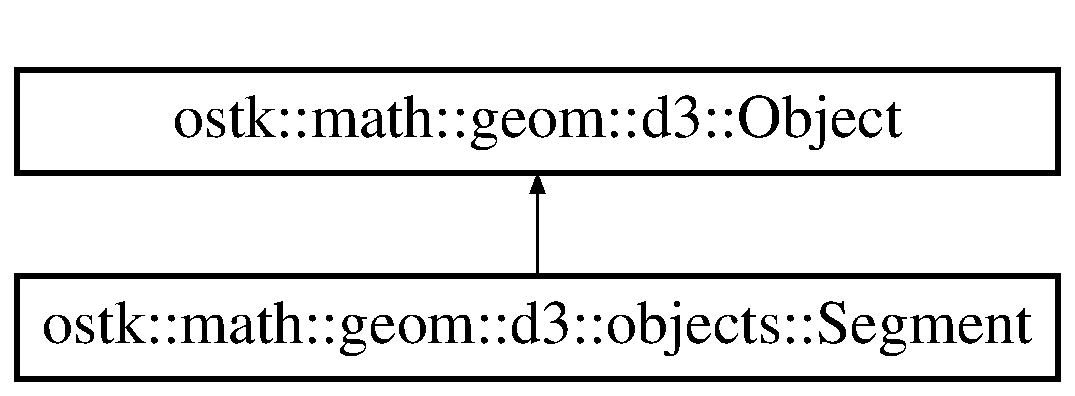
\includegraphics[height=2.000000cm]{classostk_1_1math_1_1geom_1_1d3_1_1objects_1_1_segment}
\end{center}
\end{figure}
\doxysubsection*{Public Member Functions}
\begin{DoxyCompactItemize}
\item 
\mbox{\hyperlink{classostk_1_1math_1_1geom_1_1d3_1_1objects_1_1_segment_aa2cb60ce06335a5f76120c658219494c}{Segment}} (const \mbox{\hyperlink{classostk_1_1math_1_1geom_1_1d3_1_1objects_1_1_point}{Point}} \&a\+First\+Point, const \mbox{\hyperlink{classostk_1_1math_1_1geom_1_1d3_1_1objects_1_1_point}{Point}} \&a\+Second\+Point)
\begin{DoxyCompactList}\small\item\em Constructor. \end{DoxyCompactList}\item 
virtual \mbox{\hyperlink{classostk_1_1math_1_1geom_1_1d3_1_1objects_1_1_segment}{Segment}} $\ast$ \mbox{\hyperlink{classostk_1_1math_1_1geom_1_1d3_1_1objects_1_1_segment_ab6d2215382c1b9fbdbd98501956d679d}{clone}} () const override
\begin{DoxyCompactList}\small\item\em Clone segment. \end{DoxyCompactList}\item 
bool \mbox{\hyperlink{classostk_1_1math_1_1geom_1_1d3_1_1objects_1_1_segment_ae19c34b4b4cf1ff5bb1be0835c7c064e}{operator==}} (const \mbox{\hyperlink{classostk_1_1math_1_1geom_1_1d3_1_1objects_1_1_segment}{Segment}} \&a\+Segment) const
\begin{DoxyCompactList}\small\item\em Equal to operator. \end{DoxyCompactList}\item 
bool \mbox{\hyperlink{classostk_1_1math_1_1geom_1_1d3_1_1objects_1_1_segment_a2239bed274a65f4e0f25147c15f343c7}{operator!=}} (const \mbox{\hyperlink{classostk_1_1math_1_1geom_1_1d3_1_1objects_1_1_segment}{Segment}} \&a\+Segment) const
\begin{DoxyCompactList}\small\item\em Not equal to operator. \end{DoxyCompactList}\item 
virtual bool \mbox{\hyperlink{classostk_1_1math_1_1geom_1_1d3_1_1objects_1_1_segment_ab89a57a59d50bfd6fe609e92d158e6ec}{is\+Defined}} () const override
\begin{DoxyCompactList}\small\item\em Check if segment is defined. \end{DoxyCompactList}\item 
bool \mbox{\hyperlink{classostk_1_1math_1_1geom_1_1d3_1_1objects_1_1_segment_a472767f407b4fa42ae6de7d48ccb60d0}{is\+Degenerate}} () const
\begin{DoxyCompactList}\small\item\em Check if segment is degenerate, i.\+e. its length is zero. \end{DoxyCompactList}\item 
bool \mbox{\hyperlink{classostk_1_1math_1_1geom_1_1d3_1_1objects_1_1_segment_a0d26133252b257cf0d9553ac418200c5}{intersects}} (const \mbox{\hyperlink{classostk_1_1math_1_1geom_1_1d3_1_1objects_1_1_plane}{Plane}} \&a\+Plane) const
\begin{DoxyCompactList}\small\item\em Check if segment intersects plane. \end{DoxyCompactList}\item 
bool \mbox{\hyperlink{classostk_1_1math_1_1geom_1_1d3_1_1objects_1_1_segment_a89ca3e575e43516435d8b3f6f5a6c624}{intersects}} (const \mbox{\hyperlink{classostk_1_1math_1_1geom_1_1d3_1_1objects_1_1_sphere}{Sphere}} \&a\+Sphere) const
\begin{DoxyCompactList}\small\item\em Check if segment intersects sphere. \end{DoxyCompactList}\item 
bool \mbox{\hyperlink{classostk_1_1math_1_1geom_1_1d3_1_1objects_1_1_segment_a281320eb45dcfce43caab69fb4051242}{intersects}} (const \mbox{\hyperlink{classostk_1_1math_1_1geom_1_1d3_1_1objects_1_1_ellipsoid}{Ellipsoid}} \&an\+Ellipsoid) const
\begin{DoxyCompactList}\small\item\em Check if segment intersects ellipsoid. \end{DoxyCompactList}\item 
bool \mbox{\hyperlink{classostk_1_1math_1_1geom_1_1d3_1_1objects_1_1_segment_a07d2c8bc8f734b3a99fb4f11610f9fab}{contains}} (const \mbox{\hyperlink{classostk_1_1math_1_1geom_1_1d3_1_1objects_1_1_point}{Point}} \&a\+Point) const
\begin{DoxyCompactList}\small\item\em Check if segment contains point. \end{DoxyCompactList}\item 
\mbox{\hyperlink{classostk_1_1math_1_1geom_1_1d3_1_1objects_1_1_point}{Point}} \mbox{\hyperlink{classostk_1_1math_1_1geom_1_1d3_1_1objects_1_1_segment_a0dd0944d8a53bc07b241fc933a2b023f}{get\+First\+Point}} () const
\begin{DoxyCompactList}\small\item\em Get segment first point. \end{DoxyCompactList}\item 
\mbox{\hyperlink{classostk_1_1math_1_1geom_1_1d3_1_1objects_1_1_point}{Point}} \mbox{\hyperlink{classostk_1_1math_1_1geom_1_1d3_1_1objects_1_1_segment_a194f50a9505400681ba0bb15ae999465}{get\+Second\+Point}} () const
\begin{DoxyCompactList}\small\item\em Get segment second point. \end{DoxyCompactList}\item 
\mbox{\hyperlink{classostk_1_1math_1_1geom_1_1d3_1_1objects_1_1_point}{Point}} \mbox{\hyperlink{classostk_1_1math_1_1geom_1_1d3_1_1objects_1_1_segment_a7d37a80e12053ec307dfd8e4d3973843}{get\+Center}} () const
\begin{DoxyCompactList}\small\item\em Get segment center. \end{DoxyCompactList}\item 
Vector3d \mbox{\hyperlink{classostk_1_1math_1_1geom_1_1d3_1_1objects_1_1_segment_ab708b9d0ab53ef8b15974244810a732f}{get\+Direction}} () const
\begin{DoxyCompactList}\small\item\em Get segment direction. \end{DoxyCompactList}\item 
Real \mbox{\hyperlink{classostk_1_1math_1_1geom_1_1d3_1_1objects_1_1_segment_a0f40747b4f8da2ef00b57ff0e4445968}{get\+Length}} () const
\begin{DoxyCompactList}\small\item\em Get segment length. \end{DoxyCompactList}\item 
Real \mbox{\hyperlink{classostk_1_1math_1_1geom_1_1d3_1_1objects_1_1_segment_a403915ebd6906ff29c93728b5bb8bbba}{distance\+To}} (const \mbox{\hyperlink{classostk_1_1math_1_1geom_1_1d3_1_1objects_1_1_point}{Point}} \&a\+Point) const
\begin{DoxyCompactList}\small\item\em Get distance to point. \end{DoxyCompactList}\item 
Real \mbox{\hyperlink{classostk_1_1math_1_1geom_1_1d3_1_1objects_1_1_segment_ade8414dc47f495917f43012f78e30017}{distance\+To}} (const \mbox{\hyperlink{classostk_1_1math_1_1geom_1_1d3_1_1objects_1_1_point_set}{Point\+Set}} \&a\+Point\+Set) const
\begin{DoxyCompactList}\small\item\em Get distance to point set. \end{DoxyCompactList}\item 
\mbox{\hyperlink{classostk_1_1math_1_1geom_1_1d3_1_1_intersection}{Intersection}} \mbox{\hyperlink{classostk_1_1math_1_1geom_1_1d3_1_1objects_1_1_segment_a0a2acca7fc6eb6d957a33381ab8bc6b1}{intersection\+With}} (const \mbox{\hyperlink{classostk_1_1math_1_1geom_1_1d3_1_1objects_1_1_plane}{Plane}} \&a\+Plane) const
\begin{DoxyCompactList}\small\item\em Compute intersection of segment with plane. \end{DoxyCompactList}\item 
\mbox{\hyperlink{classostk_1_1math_1_1geom_1_1d3_1_1objects_1_1_line}{Line}} \mbox{\hyperlink{classostk_1_1math_1_1geom_1_1d3_1_1objects_1_1_segment_a6f9e4f9c67f62d357fae8320dab8d48b}{to\+Line}} () const
\begin{DoxyCompactList}\small\item\em Get line from segment. \end{DoxyCompactList}\item 
virtual void \mbox{\hyperlink{classostk_1_1math_1_1geom_1_1d3_1_1objects_1_1_segment_a2c2029b6b84e984532f98dbd9a10ff1b}{print}} (std\+::ostream \&an\+Output\+Stream, bool display\+Decorators=true) const override
\begin{DoxyCompactList}\small\item\em Print segment. \end{DoxyCompactList}\item 
virtual void \mbox{\hyperlink{classostk_1_1math_1_1geom_1_1d3_1_1objects_1_1_segment_a5d2aba754d42c89224c7579944de9c4f}{apply\+Transformation}} (const \mbox{\hyperlink{classostk_1_1math_1_1geom_1_1d3_1_1_transformation}{Transformation}} \&a\+Transformation) override
\begin{DoxyCompactList}\small\item\em Apply transformation to segment. \end{DoxyCompactList}\end{DoxyCompactItemize}
\doxysubsection*{Static Public Member Functions}
\begin{DoxyCompactItemize}
\item 
static \mbox{\hyperlink{classostk_1_1math_1_1geom_1_1d3_1_1objects_1_1_segment}{Segment}} \mbox{\hyperlink{classostk_1_1math_1_1geom_1_1d3_1_1objects_1_1_segment_a488c219e6e6a137981df83b9d247f2bf}{Undefined}} ()
\begin{DoxyCompactList}\small\item\em Constructs an undefined segment. \end{DoxyCompactList}\end{DoxyCompactItemize}


\doxysubsection{Detailed Description}
\mbox{\hyperlink{classostk_1_1math_1_1geom_1_1d3_1_1objects_1_1_segment}{Segment}}. 

\begin{DoxyVerb}                        A segment is a part of a line that is bounded by two distinct end points,
                        and contains every point on the line between its endpoints.
\end{DoxyVerb}


\href{https://en.wikipedia.org/wiki/Line_segment}{\texttt{ https\+://en.\+wikipedia.\+org/wiki/\+Line\+\_\+segment}} 

\doxysubsection{Constructor \& Destructor Documentation}
\mbox{\Hypertarget{classostk_1_1math_1_1geom_1_1d3_1_1objects_1_1_segment_aa2cb60ce06335a5f76120c658219494c}\label{classostk_1_1math_1_1geom_1_1d3_1_1objects_1_1_segment_aa2cb60ce06335a5f76120c658219494c}} 
\index{ostk::math::geom::d3::objects::Segment@{ostk::math::geom::d3::objects::Segment}!Segment@{Segment}}
\index{Segment@{Segment}!ostk::math::geom::d3::objects::Segment@{ostk::math::geom::d3::objects::Segment}}
\doxysubsubsection{\texorpdfstring{Segment()}{Segment()}}
{\footnotesize\ttfamily ostk\+::math\+::geom\+::d3\+::objects\+::\+Segment\+::\+Segment (\begin{DoxyParamCaption}\item[{const \mbox{\hyperlink{classostk_1_1math_1_1geom_1_1d3_1_1objects_1_1_point}{Point}} \&}]{a\+First\+Point,  }\item[{const \mbox{\hyperlink{classostk_1_1math_1_1geom_1_1d3_1_1objects_1_1_point}{Point}} \&}]{a\+Second\+Point }\end{DoxyParamCaption})}



Constructor. 


\begin{DoxyCode}{0}
\DoxyCodeLine{\mbox{\hyperlink{classostk_1_1math_1_1geom_1_1d3_1_1objects_1_1_segment_aa2cb60ce06335a5f76120c658219494c}{Segment}} segment(\{ 0.0, 0.0, 0.0 \}, \{ 0.0, 0.0, 1.0 \}) ;}
\end{DoxyCode}



\begin{DoxyParams}[1]{Parameters}
\mbox{\texttt{ in}}  & {\em a\+First\+Point} & A first point \\
\hline
\mbox{\texttt{ in}}  & {\em a\+Second\+Point} & A second point \\
\hline
\end{DoxyParams}


\doxysubsection{Member Function Documentation}
\mbox{\Hypertarget{classostk_1_1math_1_1geom_1_1d3_1_1objects_1_1_segment_a5d2aba754d42c89224c7579944de9c4f}\label{classostk_1_1math_1_1geom_1_1d3_1_1objects_1_1_segment_a5d2aba754d42c89224c7579944de9c4f}} 
\index{ostk::math::geom::d3::objects::Segment@{ostk::math::geom::d3::objects::Segment}!applyTransformation@{applyTransformation}}
\index{applyTransformation@{applyTransformation}!ostk::math::geom::d3::objects::Segment@{ostk::math::geom::d3::objects::Segment}}
\doxysubsubsection{\texorpdfstring{applyTransformation()}{applyTransformation()}}
{\footnotesize\ttfamily void ostk\+::math\+::geom\+::d3\+::objects\+::\+Segment\+::apply\+Transformation (\begin{DoxyParamCaption}\item[{const \mbox{\hyperlink{classostk_1_1math_1_1geom_1_1d3_1_1_transformation}{Transformation}} \&}]{a\+Transformation }\end{DoxyParamCaption})\hspace{0.3cm}{\ttfamily [override]}, {\ttfamily [virtual]}}



Apply transformation to segment. 


\begin{DoxyParams}[1]{Parameters}
\mbox{\texttt{ in}}  & {\em a\+Transformation} & A transformation \\
\hline
\end{DoxyParams}


Implements \mbox{\hyperlink{classostk_1_1math_1_1geom_1_1d3_1_1_object_ae9194dd6d2bb4df09292ffc84dccdb1d}{ostk\+::math\+::geom\+::d3\+::\+Object}}.

\mbox{\Hypertarget{classostk_1_1math_1_1geom_1_1d3_1_1objects_1_1_segment_ab6d2215382c1b9fbdbd98501956d679d}\label{classostk_1_1math_1_1geom_1_1d3_1_1objects_1_1_segment_ab6d2215382c1b9fbdbd98501956d679d}} 
\index{ostk::math::geom::d3::objects::Segment@{ostk::math::geom::d3::objects::Segment}!clone@{clone}}
\index{clone@{clone}!ostk::math::geom::d3::objects::Segment@{ostk::math::geom::d3::objects::Segment}}
\doxysubsubsection{\texorpdfstring{clone()}{clone()}}
{\footnotesize\ttfamily \mbox{\hyperlink{classostk_1_1math_1_1geom_1_1d3_1_1objects_1_1_segment}{Segment}} $\ast$ ostk\+::math\+::geom\+::d3\+::objects\+::\+Segment\+::clone (\begin{DoxyParamCaption}{ }\end{DoxyParamCaption}) const\hspace{0.3cm}{\ttfamily [override]}, {\ttfamily [virtual]}}



Clone segment. 

\begin{DoxyReturn}{Returns}
Pointer to cloned segment 
\end{DoxyReturn}


Implements \mbox{\hyperlink{classostk_1_1math_1_1geom_1_1d3_1_1_object_a676013f9555f6492687f9809b2db887b}{ostk\+::math\+::geom\+::d3\+::\+Object}}.

\mbox{\Hypertarget{classostk_1_1math_1_1geom_1_1d3_1_1objects_1_1_segment_a07d2c8bc8f734b3a99fb4f11610f9fab}\label{classostk_1_1math_1_1geom_1_1d3_1_1objects_1_1_segment_a07d2c8bc8f734b3a99fb4f11610f9fab}} 
\index{ostk::math::geom::d3::objects::Segment@{ostk::math::geom::d3::objects::Segment}!contains@{contains}}
\index{contains@{contains}!ostk::math::geom::d3::objects::Segment@{ostk::math::geom::d3::objects::Segment}}
\doxysubsubsection{\texorpdfstring{contains()}{contains()}}
{\footnotesize\ttfamily bool ostk\+::math\+::geom\+::d3\+::objects\+::\+Segment\+::contains (\begin{DoxyParamCaption}\item[{const \mbox{\hyperlink{classostk_1_1math_1_1geom_1_1d3_1_1objects_1_1_point}{Point}} \&}]{a\+Point }\end{DoxyParamCaption}) const}



Check if segment contains point. 


\begin{DoxyCode}{0}
\DoxyCodeLine{\mbox{\hyperlink{classostk_1_1math_1_1geom_1_1d3_1_1objects_1_1_segment_aa2cb60ce06335a5f76120c658219494c}{Segment}} segment = ... ;}
\DoxyCodeLine{Point point = ... ;}
\DoxyCodeLine{segment.contains(point) ;}
\end{DoxyCode}



\begin{DoxyParams}[1]{Parameters}
\mbox{\texttt{ in}}  & {\em a\+Point} & A point \\
\hline
\end{DoxyParams}
\begin{DoxyReturn}{Returns}
True if segment contains point 
\end{DoxyReturn}
\mbox{\Hypertarget{classostk_1_1math_1_1geom_1_1d3_1_1objects_1_1_segment_a403915ebd6906ff29c93728b5bb8bbba}\label{classostk_1_1math_1_1geom_1_1d3_1_1objects_1_1_segment_a403915ebd6906ff29c93728b5bb8bbba}} 
\index{ostk::math::geom::d3::objects::Segment@{ostk::math::geom::d3::objects::Segment}!distanceTo@{distanceTo}}
\index{distanceTo@{distanceTo}!ostk::math::geom::d3::objects::Segment@{ostk::math::geom::d3::objects::Segment}}
\doxysubsubsection{\texorpdfstring{distanceTo()}{distanceTo()}\hspace{0.1cm}{\footnotesize\ttfamily [1/2]}}
{\footnotesize\ttfamily Real ostk\+::math\+::geom\+::d3\+::objects\+::\+Segment\+::distance\+To (\begin{DoxyParamCaption}\item[{const \mbox{\hyperlink{classostk_1_1math_1_1geom_1_1d3_1_1objects_1_1_point}{Point}} \&}]{a\+Point }\end{DoxyParamCaption}) const}



Get distance to point. 


\begin{DoxyParams}[1]{Parameters}
\mbox{\texttt{ in}}  & {\em a\+Point} & A point \\
\hline
\end{DoxyParams}
\begin{DoxyReturn}{Returns}
Distance to point 
\end{DoxyReturn}
\mbox{\Hypertarget{classostk_1_1math_1_1geom_1_1d3_1_1objects_1_1_segment_ade8414dc47f495917f43012f78e30017}\label{classostk_1_1math_1_1geom_1_1d3_1_1objects_1_1_segment_ade8414dc47f495917f43012f78e30017}} 
\index{ostk::math::geom::d3::objects::Segment@{ostk::math::geom::d3::objects::Segment}!distanceTo@{distanceTo}}
\index{distanceTo@{distanceTo}!ostk::math::geom::d3::objects::Segment@{ostk::math::geom::d3::objects::Segment}}
\doxysubsubsection{\texorpdfstring{distanceTo()}{distanceTo()}\hspace{0.1cm}{\footnotesize\ttfamily [2/2]}}
{\footnotesize\ttfamily Real ostk\+::math\+::geom\+::d3\+::objects\+::\+Segment\+::distance\+To (\begin{DoxyParamCaption}\item[{const \mbox{\hyperlink{classostk_1_1math_1_1geom_1_1d3_1_1objects_1_1_point_set}{Point\+Set}} \&}]{a\+Point\+Set }\end{DoxyParamCaption}) const}



Get distance to point set. 


\begin{DoxyParams}[1]{Parameters}
\mbox{\texttt{ in}}  & {\em a\+Point\+Set} & A point set \\
\hline
\end{DoxyParams}
\begin{DoxyReturn}{Returns}
Distance to point set 
\end{DoxyReturn}
\mbox{\Hypertarget{classostk_1_1math_1_1geom_1_1d3_1_1objects_1_1_segment_a7d37a80e12053ec307dfd8e4d3973843}\label{classostk_1_1math_1_1geom_1_1d3_1_1objects_1_1_segment_a7d37a80e12053ec307dfd8e4d3973843}} 
\index{ostk::math::geom::d3::objects::Segment@{ostk::math::geom::d3::objects::Segment}!getCenter@{getCenter}}
\index{getCenter@{getCenter}!ostk::math::geom::d3::objects::Segment@{ostk::math::geom::d3::objects::Segment}}
\doxysubsubsection{\texorpdfstring{getCenter()}{getCenter()}}
{\footnotesize\ttfamily \mbox{\hyperlink{classostk_1_1math_1_1geom_1_1d3_1_1objects_1_1_point}{Point}} ostk\+::math\+::geom\+::d3\+::objects\+::\+Segment\+::get\+Center (\begin{DoxyParamCaption}{ }\end{DoxyParamCaption}) const}



Get segment center. 


\begin{DoxyCode}{0}
\DoxyCodeLine{\mbox{\hyperlink{classostk_1_1math_1_1geom_1_1d3_1_1objects_1_1_segment_aa2cb60ce06335a5f76120c658219494c}{Segment}}(\{ 0.0, 0.0, 0.0 \}, \{ 0.0, 0.0, 2.0 \}).\mbox{\hyperlink{classostk_1_1math_1_1geom_1_1d3_1_1objects_1_1_segment_a7d37a80e12053ec307dfd8e4d3973843}{getCenter}}() ; \textcolor{comment}{// [0.0, 0.0, 1.0]}}
\end{DoxyCode}


\begin{DoxyReturn}{Returns}
\mbox{\hyperlink{classostk_1_1math_1_1geom_1_1d3_1_1objects_1_1_segment}{Segment}} center 
\end{DoxyReturn}
\mbox{\Hypertarget{classostk_1_1math_1_1geom_1_1d3_1_1objects_1_1_segment_ab708b9d0ab53ef8b15974244810a732f}\label{classostk_1_1math_1_1geom_1_1d3_1_1objects_1_1_segment_ab708b9d0ab53ef8b15974244810a732f}} 
\index{ostk::math::geom::d3::objects::Segment@{ostk::math::geom::d3::objects::Segment}!getDirection@{getDirection}}
\index{getDirection@{getDirection}!ostk::math::geom::d3::objects::Segment@{ostk::math::geom::d3::objects::Segment}}
\doxysubsubsection{\texorpdfstring{getDirection()}{getDirection()}}
{\footnotesize\ttfamily Vector3d ostk\+::math\+::geom\+::d3\+::objects\+::\+Segment\+::get\+Direction (\begin{DoxyParamCaption}{ }\end{DoxyParamCaption}) const}



Get segment direction. 


\begin{DoxyCode}{0}
\DoxyCodeLine{\mbox{\hyperlink{classostk_1_1math_1_1geom_1_1d3_1_1objects_1_1_segment_aa2cb60ce06335a5f76120c658219494c}{Segment}}(\{ 0.0, 0.0, 0.0 \}, \{ 0.0, 0.0, 2.0 \}).\mbox{\hyperlink{classostk_1_1math_1_1geom_1_1d3_1_1objects_1_1_segment_ab708b9d0ab53ef8b15974244810a732f}{getDirection}}() ; \textcolor{comment}{// [0.0, 0.0, 1.0]}}
\end{DoxyCode}


\begin{DoxyReturn}{Returns}
\mbox{\hyperlink{classostk_1_1math_1_1geom_1_1d3_1_1objects_1_1_segment}{Segment}} direction 
\end{DoxyReturn}
\mbox{\Hypertarget{classostk_1_1math_1_1geom_1_1d3_1_1objects_1_1_segment_a0dd0944d8a53bc07b241fc933a2b023f}\label{classostk_1_1math_1_1geom_1_1d3_1_1objects_1_1_segment_a0dd0944d8a53bc07b241fc933a2b023f}} 
\index{ostk::math::geom::d3::objects::Segment@{ostk::math::geom::d3::objects::Segment}!getFirstPoint@{getFirstPoint}}
\index{getFirstPoint@{getFirstPoint}!ostk::math::geom::d3::objects::Segment@{ostk::math::geom::d3::objects::Segment}}
\doxysubsubsection{\texorpdfstring{getFirstPoint()}{getFirstPoint()}}
{\footnotesize\ttfamily \mbox{\hyperlink{classostk_1_1math_1_1geom_1_1d3_1_1objects_1_1_point}{Point}} ostk\+::math\+::geom\+::d3\+::objects\+::\+Segment\+::get\+First\+Point (\begin{DoxyParamCaption}{ }\end{DoxyParamCaption}) const}



Get segment first point. 


\begin{DoxyCode}{0}
\DoxyCodeLine{\mbox{\hyperlink{classostk_1_1math_1_1geom_1_1d3_1_1objects_1_1_segment_aa2cb60ce06335a5f76120c658219494c}{Segment}}(\{ 0.0, 0.0, 0.0 \}, \{ 0.0, 0.0, 1.0 \}).\mbox{\hyperlink{classostk_1_1math_1_1geom_1_1d3_1_1objects_1_1_segment_a0dd0944d8a53bc07b241fc933a2b023f}{getFirstPoint}}() ; \textcolor{comment}{// [0.0, 0.0, 0.0]}}
\end{DoxyCode}


\begin{DoxyReturn}{Returns}
\mbox{\hyperlink{classostk_1_1math_1_1geom_1_1d3_1_1objects_1_1_segment}{Segment}} first point 
\end{DoxyReturn}
\mbox{\Hypertarget{classostk_1_1math_1_1geom_1_1d3_1_1objects_1_1_segment_a0f40747b4f8da2ef00b57ff0e4445968}\label{classostk_1_1math_1_1geom_1_1d3_1_1objects_1_1_segment_a0f40747b4f8da2ef00b57ff0e4445968}} 
\index{ostk::math::geom::d3::objects::Segment@{ostk::math::geom::d3::objects::Segment}!getLength@{getLength}}
\index{getLength@{getLength}!ostk::math::geom::d3::objects::Segment@{ostk::math::geom::d3::objects::Segment}}
\doxysubsubsection{\texorpdfstring{getLength()}{getLength()}}
{\footnotesize\ttfamily Real ostk\+::math\+::geom\+::d3\+::objects\+::\+Segment\+::get\+Length (\begin{DoxyParamCaption}{ }\end{DoxyParamCaption}) const}



Get segment length. 


\begin{DoxyCode}{0}
\DoxyCodeLine{\mbox{\hyperlink{classostk_1_1math_1_1geom_1_1d3_1_1objects_1_1_segment_aa2cb60ce06335a5f76120c658219494c}{Segment}}(\{ 0.0, 0.0, 0.0 \}, \{ 0.0, 0.0, 2.0 \}).\mbox{\hyperlink{classostk_1_1math_1_1geom_1_1d3_1_1objects_1_1_segment_a0f40747b4f8da2ef00b57ff0e4445968}{getLength}}() ; \textcolor{comment}{// 2.0}}
\end{DoxyCode}


\begin{DoxyReturn}{Returns}
\mbox{\hyperlink{classostk_1_1math_1_1geom_1_1d3_1_1objects_1_1_segment}{Segment}} length 
\end{DoxyReturn}
\mbox{\Hypertarget{classostk_1_1math_1_1geom_1_1d3_1_1objects_1_1_segment_a194f50a9505400681ba0bb15ae999465}\label{classostk_1_1math_1_1geom_1_1d3_1_1objects_1_1_segment_a194f50a9505400681ba0bb15ae999465}} 
\index{ostk::math::geom::d3::objects::Segment@{ostk::math::geom::d3::objects::Segment}!getSecondPoint@{getSecondPoint}}
\index{getSecondPoint@{getSecondPoint}!ostk::math::geom::d3::objects::Segment@{ostk::math::geom::d3::objects::Segment}}
\doxysubsubsection{\texorpdfstring{getSecondPoint()}{getSecondPoint()}}
{\footnotesize\ttfamily \mbox{\hyperlink{classostk_1_1math_1_1geom_1_1d3_1_1objects_1_1_point}{Point}} ostk\+::math\+::geom\+::d3\+::objects\+::\+Segment\+::get\+Second\+Point (\begin{DoxyParamCaption}{ }\end{DoxyParamCaption}) const}



Get segment second point. 


\begin{DoxyCode}{0}
\DoxyCodeLine{\mbox{\hyperlink{classostk_1_1math_1_1geom_1_1d3_1_1objects_1_1_segment_aa2cb60ce06335a5f76120c658219494c}{Segment}}(\{ 0.0, 0.0, 0.0 \}, \{ 0.0, 0.0, 1.0 \}).\mbox{\hyperlink{classostk_1_1math_1_1geom_1_1d3_1_1objects_1_1_segment_a194f50a9505400681ba0bb15ae999465}{getSecondPoint}}() ; \textcolor{comment}{// [0.0, 0.0, 1.0]}}
\end{DoxyCode}


\begin{DoxyReturn}{Returns}
\mbox{\hyperlink{classostk_1_1math_1_1geom_1_1d3_1_1objects_1_1_segment}{Segment}} second point 
\end{DoxyReturn}
\mbox{\Hypertarget{classostk_1_1math_1_1geom_1_1d3_1_1objects_1_1_segment_a0a2acca7fc6eb6d957a33381ab8bc6b1}\label{classostk_1_1math_1_1geom_1_1d3_1_1objects_1_1_segment_a0a2acca7fc6eb6d957a33381ab8bc6b1}} 
\index{ostk::math::geom::d3::objects::Segment@{ostk::math::geom::d3::objects::Segment}!intersectionWith@{intersectionWith}}
\index{intersectionWith@{intersectionWith}!ostk::math::geom::d3::objects::Segment@{ostk::math::geom::d3::objects::Segment}}
\doxysubsubsection{\texorpdfstring{intersectionWith()}{intersectionWith()}}
{\footnotesize\ttfamily \mbox{\hyperlink{classostk_1_1math_1_1geom_1_1d3_1_1_intersection}{Intersection}} ostk\+::math\+::geom\+::d3\+::objects\+::\+Segment\+::intersection\+With (\begin{DoxyParamCaption}\item[{const \mbox{\hyperlink{classostk_1_1math_1_1geom_1_1d3_1_1objects_1_1_plane}{Plane}} \&}]{a\+Plane }\end{DoxyParamCaption}) const}



Compute intersection of segment with plane. 


\begin{DoxyParams}[1]{Parameters}
\mbox{\texttt{ in}}  & {\em a\+Plane} & A plane \\
\hline
\end{DoxyParams}
\begin{DoxyReturn}{Returns}
\mbox{\hyperlink{classostk_1_1math_1_1geom_1_1d3_1_1_intersection}{Intersection}} of segment with plane 
\end{DoxyReturn}
\mbox{\Hypertarget{classostk_1_1math_1_1geom_1_1d3_1_1objects_1_1_segment_a281320eb45dcfce43caab69fb4051242}\label{classostk_1_1math_1_1geom_1_1d3_1_1objects_1_1_segment_a281320eb45dcfce43caab69fb4051242}} 
\index{ostk::math::geom::d3::objects::Segment@{ostk::math::geom::d3::objects::Segment}!intersects@{intersects}}
\index{intersects@{intersects}!ostk::math::geom::d3::objects::Segment@{ostk::math::geom::d3::objects::Segment}}
\doxysubsubsection{\texorpdfstring{intersects()}{intersects()}\hspace{0.1cm}{\footnotesize\ttfamily [1/3]}}
{\footnotesize\ttfamily bool ostk\+::math\+::geom\+::d3\+::objects\+::\+Segment\+::intersects (\begin{DoxyParamCaption}\item[{const \mbox{\hyperlink{classostk_1_1math_1_1geom_1_1d3_1_1objects_1_1_ellipsoid}{Ellipsoid}} \&}]{an\+Ellipsoid }\end{DoxyParamCaption}) const}



Check if segment intersects ellipsoid. 


\begin{DoxyCode}{0}
\DoxyCodeLine{\mbox{\hyperlink{classostk_1_1math_1_1geom_1_1d3_1_1objects_1_1_segment_aa2cb60ce06335a5f76120c658219494c}{Segment}} segment = ... ;}
\DoxyCodeLine{Ellipsoid ellipsoid = ... ;}
\DoxyCodeLine{segment.intersects(ellipsoid) ;}
\end{DoxyCode}



\begin{DoxyParams}[1]{Parameters}
\mbox{\texttt{ in}}  & {\em an\+Ellipsoid} & An ellipsoid \\
\hline
\end{DoxyParams}
\begin{DoxyReturn}{Returns}
True if segment intersects ellipsoid 
\end{DoxyReturn}
\mbox{\Hypertarget{classostk_1_1math_1_1geom_1_1d3_1_1objects_1_1_segment_a0d26133252b257cf0d9553ac418200c5}\label{classostk_1_1math_1_1geom_1_1d3_1_1objects_1_1_segment_a0d26133252b257cf0d9553ac418200c5}} 
\index{ostk::math::geom::d3::objects::Segment@{ostk::math::geom::d3::objects::Segment}!intersects@{intersects}}
\index{intersects@{intersects}!ostk::math::geom::d3::objects::Segment@{ostk::math::geom::d3::objects::Segment}}
\doxysubsubsection{\texorpdfstring{intersects()}{intersects()}\hspace{0.1cm}{\footnotesize\ttfamily [2/3]}}
{\footnotesize\ttfamily bool ostk\+::math\+::geom\+::d3\+::objects\+::\+Segment\+::intersects (\begin{DoxyParamCaption}\item[{const \mbox{\hyperlink{classostk_1_1math_1_1geom_1_1d3_1_1objects_1_1_plane}{Plane}} \&}]{a\+Plane }\end{DoxyParamCaption}) const}



Check if segment intersects plane. 


\begin{DoxyCode}{0}
\DoxyCodeLine{\mbox{\hyperlink{classostk_1_1math_1_1geom_1_1d3_1_1objects_1_1_segment_aa2cb60ce06335a5f76120c658219494c}{Segment}} segment = ... ;}
\DoxyCodeLine{Plane plane = ... ;}
\DoxyCodeLine{segment.intersects(plane) ;}
\end{DoxyCode}



\begin{DoxyParams}[1]{Parameters}
\mbox{\texttt{ in}}  & {\em a\+Plane} & A plane \\
\hline
\end{DoxyParams}
\begin{DoxyReturn}{Returns}
True if segment intersects plane 
\end{DoxyReturn}
\mbox{\Hypertarget{classostk_1_1math_1_1geom_1_1d3_1_1objects_1_1_segment_a89ca3e575e43516435d8b3f6f5a6c624}\label{classostk_1_1math_1_1geom_1_1d3_1_1objects_1_1_segment_a89ca3e575e43516435d8b3f6f5a6c624}} 
\index{ostk::math::geom::d3::objects::Segment@{ostk::math::geom::d3::objects::Segment}!intersects@{intersects}}
\index{intersects@{intersects}!ostk::math::geom::d3::objects::Segment@{ostk::math::geom::d3::objects::Segment}}
\doxysubsubsection{\texorpdfstring{intersects()}{intersects()}\hspace{0.1cm}{\footnotesize\ttfamily [3/3]}}
{\footnotesize\ttfamily bool ostk\+::math\+::geom\+::d3\+::objects\+::\+Segment\+::intersects (\begin{DoxyParamCaption}\item[{const \mbox{\hyperlink{classostk_1_1math_1_1geom_1_1d3_1_1objects_1_1_sphere}{Sphere}} \&}]{a\+Sphere }\end{DoxyParamCaption}) const}



Check if segment intersects sphere. 


\begin{DoxyCode}{0}
\DoxyCodeLine{\mbox{\hyperlink{classostk_1_1math_1_1geom_1_1d3_1_1objects_1_1_segment_aa2cb60ce06335a5f76120c658219494c}{Segment}} segment = ... ;}
\DoxyCodeLine{Sphere sphere = ... ;}
\DoxyCodeLine{segment.intersects(sphere) ;}
\end{DoxyCode}



\begin{DoxyParams}[1]{Parameters}
\mbox{\texttt{ in}}  & {\em a\+Sphere} & A sphere \\
\hline
\end{DoxyParams}
\begin{DoxyReturn}{Returns}
True if segment intersects sphere 
\end{DoxyReturn}
\mbox{\Hypertarget{classostk_1_1math_1_1geom_1_1d3_1_1objects_1_1_segment_ab89a57a59d50bfd6fe609e92d158e6ec}\label{classostk_1_1math_1_1geom_1_1d3_1_1objects_1_1_segment_ab89a57a59d50bfd6fe609e92d158e6ec}} 
\index{ostk::math::geom::d3::objects::Segment@{ostk::math::geom::d3::objects::Segment}!isDefined@{isDefined}}
\index{isDefined@{isDefined}!ostk::math::geom::d3::objects::Segment@{ostk::math::geom::d3::objects::Segment}}
\doxysubsubsection{\texorpdfstring{isDefined()}{isDefined()}}
{\footnotesize\ttfamily bool ostk\+::math\+::geom\+::d3\+::objects\+::\+Segment\+::is\+Defined (\begin{DoxyParamCaption}{ }\end{DoxyParamCaption}) const\hspace{0.3cm}{\ttfamily [override]}, {\ttfamily [virtual]}}



Check if segment is defined. 


\begin{DoxyCode}{0}
\DoxyCodeLine{\mbox{\hyperlink{classostk_1_1math_1_1geom_1_1d3_1_1objects_1_1_segment_aa2cb60ce06335a5f76120c658219494c}{Segment}}(\{ 0.0, 0.0, 0.0 \}, \{ 0.0, 0.0, 1.0 \}).\mbox{\hyperlink{classostk_1_1math_1_1geom_1_1d3_1_1objects_1_1_segment_ab89a57a59d50bfd6fe609e92d158e6ec}{isDefined}}() ; \textcolor{comment}{// True}}
\end{DoxyCode}


\begin{DoxyReturn}{Returns}
True if segment is defined 
\end{DoxyReturn}


Implements \mbox{\hyperlink{classostk_1_1math_1_1geom_1_1d3_1_1_object_a271a1964cd208be85ce9a0a429395ad8}{ostk\+::math\+::geom\+::d3\+::\+Object}}.

\mbox{\Hypertarget{classostk_1_1math_1_1geom_1_1d3_1_1objects_1_1_segment_a472767f407b4fa42ae6de7d48ccb60d0}\label{classostk_1_1math_1_1geom_1_1d3_1_1objects_1_1_segment_a472767f407b4fa42ae6de7d48ccb60d0}} 
\index{ostk::math::geom::d3::objects::Segment@{ostk::math::geom::d3::objects::Segment}!isDegenerate@{isDegenerate}}
\index{isDegenerate@{isDegenerate}!ostk::math::geom::d3::objects::Segment@{ostk::math::geom::d3::objects::Segment}}
\doxysubsubsection{\texorpdfstring{isDegenerate()}{isDegenerate()}}
{\footnotesize\ttfamily bool ostk\+::math\+::geom\+::d3\+::objects\+::\+Segment\+::is\+Degenerate (\begin{DoxyParamCaption}{ }\end{DoxyParamCaption}) const}



Check if segment is degenerate, i.\+e. its length is zero. 


\begin{DoxyCode}{0}
\DoxyCodeLine{\mbox{\hyperlink{classostk_1_1math_1_1geom_1_1d3_1_1objects_1_1_segment_aa2cb60ce06335a5f76120c658219494c}{Segment}}(\{ 0.0, 0.0, 0.0 \}, \{ 0.0, 0.0, 0.0 \}).\mbox{\hyperlink{classostk_1_1math_1_1geom_1_1d3_1_1objects_1_1_segment_a472767f407b4fa42ae6de7d48ccb60d0}{isDegenerate}}() ; \textcolor{comment}{// True}}
\end{DoxyCode}


\begin{DoxyReturn}{Returns}
True if segment is degenerate 
\end{DoxyReturn}
\mbox{\Hypertarget{classostk_1_1math_1_1geom_1_1d3_1_1objects_1_1_segment_a2239bed274a65f4e0f25147c15f343c7}\label{classostk_1_1math_1_1geom_1_1d3_1_1objects_1_1_segment_a2239bed274a65f4e0f25147c15f343c7}} 
\index{ostk::math::geom::d3::objects::Segment@{ostk::math::geom::d3::objects::Segment}!operator"!=@{operator"!=}}
\index{operator"!=@{operator"!=}!ostk::math::geom::d3::objects::Segment@{ostk::math::geom::d3::objects::Segment}}
\doxysubsubsection{\texorpdfstring{operator"!=()}{operator!=()}}
{\footnotesize\ttfamily bool ostk\+::math\+::geom\+::d3\+::objects\+::\+Segment\+::operator!= (\begin{DoxyParamCaption}\item[{const \mbox{\hyperlink{classostk_1_1math_1_1geom_1_1d3_1_1objects_1_1_segment}{Segment}} \&}]{a\+Segment }\end{DoxyParamCaption}) const}



Not equal to operator. 


\begin{DoxyCode}{0}
\DoxyCodeLine{\mbox{\hyperlink{classostk_1_1math_1_1geom_1_1d3_1_1objects_1_1_segment_aa2cb60ce06335a5f76120c658219494c}{Segment}}(\{ 0.0, 0.0, 0.0 \}, \{ 0.0, 0.0, 1.0 \}) != \mbox{\hyperlink{classostk_1_1math_1_1geom_1_1d3_1_1objects_1_1_segment_aa2cb60ce06335a5f76120c658219494c}{Segment}}(\{ 0.0, 0.0, 0.0 \}, \{ 0.0, 0.0, 2.0 \}) ; \textcolor{comment}{// True}}
\end{DoxyCode}



\begin{DoxyParams}[1]{Parameters}
\mbox{\texttt{ in}}  & {\em a\+Segment} & A segment \\
\hline
\end{DoxyParams}
\begin{DoxyReturn}{Returns}
True if segments are not equal 
\end{DoxyReturn}
\mbox{\Hypertarget{classostk_1_1math_1_1geom_1_1d3_1_1objects_1_1_segment_ae19c34b4b4cf1ff5bb1be0835c7c064e}\label{classostk_1_1math_1_1geom_1_1d3_1_1objects_1_1_segment_ae19c34b4b4cf1ff5bb1be0835c7c064e}} 
\index{ostk::math::geom::d3::objects::Segment@{ostk::math::geom::d3::objects::Segment}!operator==@{operator==}}
\index{operator==@{operator==}!ostk::math::geom::d3::objects::Segment@{ostk::math::geom::d3::objects::Segment}}
\doxysubsubsection{\texorpdfstring{operator==()}{operator==()}}
{\footnotesize\ttfamily bool ostk\+::math\+::geom\+::d3\+::objects\+::\+Segment\+::operator== (\begin{DoxyParamCaption}\item[{const \mbox{\hyperlink{classostk_1_1math_1_1geom_1_1d3_1_1objects_1_1_segment}{Segment}} \&}]{a\+Segment }\end{DoxyParamCaption}) const}



Equal to operator. 


\begin{DoxyCode}{0}
\DoxyCodeLine{\mbox{\hyperlink{classostk_1_1math_1_1geom_1_1d3_1_1objects_1_1_segment_aa2cb60ce06335a5f76120c658219494c}{Segment}}(\{ 0.0, 0.0, 0.0 \}, \{ 0.0, 0.0, 1.0 \}) == \mbox{\hyperlink{classostk_1_1math_1_1geom_1_1d3_1_1objects_1_1_segment_aa2cb60ce06335a5f76120c658219494c}{Segment}}(\{ 0.0, 0.0, 0.0 \}, \{ 0.0, 0.0, 1.0 \}) ; \textcolor{comment}{// True}}
\end{DoxyCode}



\begin{DoxyParams}[1]{Parameters}
\mbox{\texttt{ in}}  & {\em a\+Segment} & A segment \\
\hline
\end{DoxyParams}
\begin{DoxyReturn}{Returns}
True if segments are equal 
\end{DoxyReturn}
\mbox{\Hypertarget{classostk_1_1math_1_1geom_1_1d3_1_1objects_1_1_segment_a2c2029b6b84e984532f98dbd9a10ff1b}\label{classostk_1_1math_1_1geom_1_1d3_1_1objects_1_1_segment_a2c2029b6b84e984532f98dbd9a10ff1b}} 
\index{ostk::math::geom::d3::objects::Segment@{ostk::math::geom::d3::objects::Segment}!print@{print}}
\index{print@{print}!ostk::math::geom::d3::objects::Segment@{ostk::math::geom::d3::objects::Segment}}
\doxysubsubsection{\texorpdfstring{print()}{print()}}
{\footnotesize\ttfamily void ostk\+::math\+::geom\+::d3\+::objects\+::\+Segment\+::print (\begin{DoxyParamCaption}\item[{std\+::ostream \&}]{an\+Output\+Stream,  }\item[{bool}]{display\+Decorators = {\ttfamily true} }\end{DoxyParamCaption}) const\hspace{0.3cm}{\ttfamily [override]}, {\ttfamily [virtual]}}



Print segment. 


\begin{DoxyParams}[1]{Parameters}
\mbox{\texttt{ in}}  & {\em an\+Output\+Stream} & An output stream \\
\hline
\mbox{\texttt{ in}}  & {\em (optional)} & display\+Decorators If true, display decorators \\
\hline
\end{DoxyParams}


Implements \mbox{\hyperlink{classostk_1_1math_1_1geom_1_1d3_1_1_object_ab2a2a782503b97d1cecabdfedc636fce}{ostk\+::math\+::geom\+::d3\+::\+Object}}.

\mbox{\Hypertarget{classostk_1_1math_1_1geom_1_1d3_1_1objects_1_1_segment_a6f9e4f9c67f62d357fae8320dab8d48b}\label{classostk_1_1math_1_1geom_1_1d3_1_1objects_1_1_segment_a6f9e4f9c67f62d357fae8320dab8d48b}} 
\index{ostk::math::geom::d3::objects::Segment@{ostk::math::geom::d3::objects::Segment}!toLine@{toLine}}
\index{toLine@{toLine}!ostk::math::geom::d3::objects::Segment@{ostk::math::geom::d3::objects::Segment}}
\doxysubsubsection{\texorpdfstring{toLine()}{toLine()}}
{\footnotesize\ttfamily \mbox{\hyperlink{classostk_1_1math_1_1geom_1_1d3_1_1objects_1_1_line}{Line}} ostk\+::math\+::geom\+::d3\+::objects\+::\+Segment\+::to\+Line (\begin{DoxyParamCaption}{ }\end{DoxyParamCaption}) const}



Get line from segment. 

\begin{DoxyReturn}{Returns}
\mbox{\hyperlink{classostk_1_1math_1_1geom_1_1d3_1_1objects_1_1_line}{Line}} 
\end{DoxyReturn}
\mbox{\Hypertarget{classostk_1_1math_1_1geom_1_1d3_1_1objects_1_1_segment_a488c219e6e6a137981df83b9d247f2bf}\label{classostk_1_1math_1_1geom_1_1d3_1_1objects_1_1_segment_a488c219e6e6a137981df83b9d247f2bf}} 
\index{ostk::math::geom::d3::objects::Segment@{ostk::math::geom::d3::objects::Segment}!Undefined@{Undefined}}
\index{Undefined@{Undefined}!ostk::math::geom::d3::objects::Segment@{ostk::math::geom::d3::objects::Segment}}
\doxysubsubsection{\texorpdfstring{Undefined()}{Undefined()}}
{\footnotesize\ttfamily \mbox{\hyperlink{classostk_1_1math_1_1geom_1_1d3_1_1objects_1_1_segment}{Segment}} ostk\+::math\+::geom\+::d3\+::objects\+::\+Segment\+::\+Undefined (\begin{DoxyParamCaption}{ }\end{DoxyParamCaption})\hspace{0.3cm}{\ttfamily [static]}}



Constructs an undefined segment. 


\begin{DoxyCode}{0}
\DoxyCodeLine{\mbox{\hyperlink{classostk_1_1math_1_1geom_1_1d3_1_1objects_1_1_segment_aa2cb60ce06335a5f76120c658219494c}{Segment}} segment = \mbox{\hyperlink{classostk_1_1math_1_1geom_1_1d3_1_1objects_1_1_segment_a488c219e6e6a137981df83b9d247f2bf}{Segment::Undefined}}() ; \textcolor{comment}{// Undefined}}
\end{DoxyCode}


\begin{DoxyReturn}{Returns}
Undefined segment 
\end{DoxyReturn}


The documentation for this class was generated from the following files\+:\begin{DoxyCompactItemize}
\item 
include/\+Open\+Space\+Toolkit/\+Mathematics/\+Geometry/3\+D/\+Objects/\mbox{\hyperlink{3_d_2_objects_2_segment_8hpp}{Segment.\+hpp}}\item 
src/\+Open\+Space\+Toolkit/\+Mathematics/\+Geometry/3\+D/\+Objects/\mbox{\hyperlink{3_d_2_objects_2_segment_8cpp}{Segment.\+cpp}}\end{DoxyCompactItemize}

\hypertarget{classostk_1_1math_1_1geom_1_1d2_1_1objects_1_1_segment}{}\section{ostk\+:\+:math\+:\+:geom\+:\+:d2\+:\+:objects\+:\+:Segment Class Reference}
\label{classostk_1_1math_1_1geom_1_1d2_1_1objects_1_1_segment}\index{ostk\+::math\+::geom\+::d2\+::objects\+::\+Segment@{ostk\+::math\+::geom\+::d2\+::objects\+::\+Segment}}


\hyperlink{classostk_1_1math_1_1geom_1_1d2_1_1objects_1_1_segment}{Segment}.  




{\ttfamily \#include $<$Segment.\+hpp$>$}

Inheritance diagram for ostk\+:\+:math\+:\+:geom\+:\+:d2\+:\+:objects\+:\+:Segment\+:\begin{figure}[H]
\begin{center}
\leavevmode
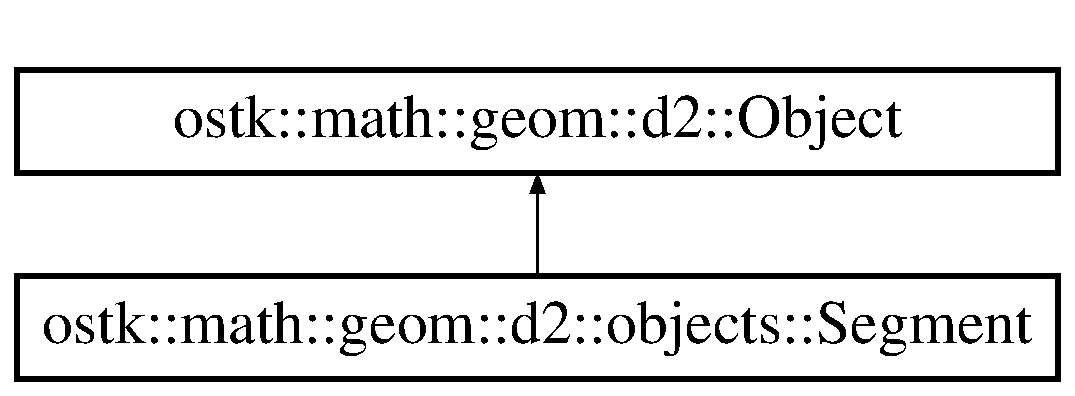
\includegraphics[height=2.000000cm]{classostk_1_1math_1_1geom_1_1d2_1_1objects_1_1_segment}
\end{center}
\end{figure}
\subsection*{Public Member Functions}
\begin{DoxyCompactItemize}
\item 
\hyperlink{classostk_1_1math_1_1geom_1_1d2_1_1objects_1_1_segment_a56c91f22315d7cefe9d5e9973330028d}{Segment} (const \hyperlink{classostk_1_1math_1_1geom_1_1d2_1_1objects_1_1_point}{Point} \&a\+First\+Point, const \hyperlink{classostk_1_1math_1_1geom_1_1d2_1_1objects_1_1_point}{Point} \&a\+Second\+Point)
\begin{DoxyCompactList}\small\item\em Constructor. \end{DoxyCompactList}\item 
virtual \hyperlink{classostk_1_1math_1_1geom_1_1d2_1_1objects_1_1_segment}{Segment} $\ast$ \hyperlink{classostk_1_1math_1_1geom_1_1d2_1_1objects_1_1_segment_ad0ba7ee144638335e4f02da0de38beab}{clone} () const override
\begin{DoxyCompactList}\small\item\em Clone segment. \end{DoxyCompactList}\item 
bool \hyperlink{classostk_1_1math_1_1geom_1_1d2_1_1objects_1_1_segment_a1b6b81c43a1f80a4ddd07ac62943db24}{operator==} (const \hyperlink{classostk_1_1math_1_1geom_1_1d2_1_1objects_1_1_segment}{Segment} \&a\+Segment) const
\begin{DoxyCompactList}\small\item\em Equal to operator. \end{DoxyCompactList}\item 
bool \hyperlink{classostk_1_1math_1_1geom_1_1d2_1_1objects_1_1_segment_a3a2de88cdbd141be1bfd22945e3fa100}{operator!=} (const \hyperlink{classostk_1_1math_1_1geom_1_1d2_1_1objects_1_1_segment}{Segment} \&a\+Segment) const
\begin{DoxyCompactList}\small\item\em Not equal to operator. \end{DoxyCompactList}\item 
virtual bool \hyperlink{classostk_1_1math_1_1geom_1_1d2_1_1objects_1_1_segment_a4e7397f14fd36b0aecd7afddd4fddf84}{is\+Defined} () const override
\begin{DoxyCompactList}\small\item\em Check if segment is defined. \end{DoxyCompactList}\item 
bool \hyperlink{classostk_1_1math_1_1geom_1_1d2_1_1objects_1_1_segment_a35a46e06daf7d791b0069641cf684f91}{is\+Degenerate} () const
\begin{DoxyCompactList}\small\item\em Check if segment is degenerate, i.\+e. its length is zero. \end{DoxyCompactList}\item 
bool \hyperlink{classostk_1_1math_1_1geom_1_1d2_1_1objects_1_1_segment_a08468b912471a18d29062b96968afc2f}{contains} (const \hyperlink{classostk_1_1math_1_1geom_1_1d2_1_1objects_1_1_point}{Point} \&a\+Point) const
\begin{DoxyCompactList}\small\item\em Check if segment contains point. \end{DoxyCompactList}\item 
bool \hyperlink{classostk_1_1math_1_1geom_1_1d2_1_1objects_1_1_segment_afd9fea7d6b73c7136ddb1246e20134d3}{contains} (const \hyperlink{classostk_1_1math_1_1geom_1_1d2_1_1objects_1_1_point_set}{Point\+Set} \&a\+Point\+Set) const
\begin{DoxyCompactList}\small\item\em Check if segment contains point set. \end{DoxyCompactList}\item 
\hyperlink{classostk_1_1math_1_1geom_1_1d2_1_1objects_1_1_point}{Point} \hyperlink{classostk_1_1math_1_1geom_1_1d2_1_1objects_1_1_segment_a8c91be64413c5944403dcd61daa141ae}{get\+First\+Point} () const
\begin{DoxyCompactList}\small\item\em Get segment first point. \end{DoxyCompactList}\item 
\hyperlink{classostk_1_1math_1_1geom_1_1d2_1_1objects_1_1_point}{Point} \hyperlink{classostk_1_1math_1_1geom_1_1d2_1_1objects_1_1_segment_ac2ff9eb997a2cd304b9162dd800bce01}{get\+Second\+Point} () const
\begin{DoxyCompactList}\small\item\em Get segment second point. \end{DoxyCompactList}\item 
\hyperlink{classostk_1_1math_1_1geom_1_1d2_1_1objects_1_1_point}{Point} \hyperlink{classostk_1_1math_1_1geom_1_1d2_1_1objects_1_1_segment_a691c0ef8268b6c3628e1cb69beb9ed74}{get\+Center} () const
\begin{DoxyCompactList}\small\item\em Get segment center. \end{DoxyCompactList}\item 
Vector2d \hyperlink{classostk_1_1math_1_1geom_1_1d2_1_1objects_1_1_segment_a92754ce55fb91c186fbe06db876425f9}{get\+Direction} () const
\begin{DoxyCompactList}\small\item\em Get segment direction. \end{DoxyCompactList}\item 
Real \hyperlink{classostk_1_1math_1_1geom_1_1d2_1_1objects_1_1_segment_a9e6dcd2b0d921c755b6980f457ed7f3e}{get\+Length} () const
\begin{DoxyCompactList}\small\item\em Get segment length. \end{DoxyCompactList}\item 
Real \hyperlink{classostk_1_1math_1_1geom_1_1d2_1_1objects_1_1_segment_a86ccd1f27b77bb7bc08c6461ccdf67b4}{distance\+To} (const \hyperlink{classostk_1_1math_1_1geom_1_1d2_1_1objects_1_1_point}{Point} \&a\+Point) const
\begin{DoxyCompactList}\small\item\em Get distance to point. \end{DoxyCompactList}\item 
Real \hyperlink{classostk_1_1math_1_1geom_1_1d2_1_1objects_1_1_segment_ab1619a8228472bd21629ad889d8eec99}{distance\+To} (const \hyperlink{classostk_1_1math_1_1geom_1_1d2_1_1objects_1_1_point_set}{Point\+Set} \&a\+Point\+Set) const
\begin{DoxyCompactList}\small\item\em Get distance to point set. \end{DoxyCompactList}\item 
\hyperlink{classostk_1_1math_1_1geom_1_1d2_1_1objects_1_1_line}{Line} \hyperlink{classostk_1_1math_1_1geom_1_1d2_1_1objects_1_1_segment_a0a630cfcf9111d168924035d768dd38a}{to\+Line} () const
\begin{DoxyCompactList}\small\item\em Get line from segment. \end{DoxyCompactList}\item 
virtual String \hyperlink{classostk_1_1math_1_1geom_1_1d2_1_1objects_1_1_segment_ac302430065e10f1f281bb8782a904673}{to\+String} (const \hyperlink{classostk_1_1math_1_1geom_1_1d2_1_1_object_aa76f9e30caebf4005bafbdff447f66cf}{Object\+::\+Format} \&a\+Format=\hyperlink{classostk_1_1math_1_1geom_1_1d2_1_1_object_aa76f9e30caebf4005bafbdff447f66cfaeb6d8ae6f20283755b339c0dc273988b}{Object\+::\+Format\+::\+Standard}, const Integer \&a\+Precision=Integer\+::\+Undefined()) const override
\begin{DoxyCompactList}\small\item\em Get string representation. \end{DoxyCompactList}\item 
virtual void \hyperlink{classostk_1_1math_1_1geom_1_1d2_1_1objects_1_1_segment_a475ba5efb353218779018b9be88be276}{print} (std\+::ostream \&an\+Output\+Stream, bool display\+Decorators=true) const override
\begin{DoxyCompactList}\small\item\em Print segment. \end{DoxyCompactList}\item 
virtual void \hyperlink{classostk_1_1math_1_1geom_1_1d2_1_1objects_1_1_segment_afbd5fe1b8136f738a0e93b934b290394}{apply\+Transformation} (const \hyperlink{classostk_1_1math_1_1geom_1_1d2_1_1_transformation}{Transformation} \&a\+Transformation) override
\begin{DoxyCompactList}\small\item\em Apply transformation to segment. \end{DoxyCompactList}\end{DoxyCompactItemize}
\subsection*{Static Public Member Functions}
\begin{DoxyCompactItemize}
\item 
static \hyperlink{classostk_1_1math_1_1geom_1_1d2_1_1objects_1_1_segment}{Segment} \hyperlink{classostk_1_1math_1_1geom_1_1d2_1_1objects_1_1_segment_a44d3a5817296d96bf82ebbc459055025}{Undefined} ()
\begin{DoxyCompactList}\small\item\em Constructs an undefined segment. \end{DoxyCompactList}\end{DoxyCompactItemize}
\subsection*{Additional Inherited Members}


\subsection{Detailed Description}
\hyperlink{classostk_1_1math_1_1geom_1_1d2_1_1objects_1_1_segment}{Segment}. 

A segment is a part of a line that is bounded by two distinct end points, and contains every point on the line between its endpoints.

https\+://en.wikipedia.\+org/wiki/\+Line\+\_\+segment 

\subsection{Constructor \& Destructor Documentation}
\mbox{\Hypertarget{classostk_1_1math_1_1geom_1_1d2_1_1objects_1_1_segment_a56c91f22315d7cefe9d5e9973330028d}\label{classostk_1_1math_1_1geom_1_1d2_1_1objects_1_1_segment_a56c91f22315d7cefe9d5e9973330028d}} 
\index{ostk\+::math\+::geom\+::d2\+::objects\+::\+Segment@{ostk\+::math\+::geom\+::d2\+::objects\+::\+Segment}!Segment@{Segment}}
\index{Segment@{Segment}!ostk\+::math\+::geom\+::d2\+::objects\+::\+Segment@{ostk\+::math\+::geom\+::d2\+::objects\+::\+Segment}}
\subsubsection{\texorpdfstring{Segment()}{Segment()}}
{\footnotesize\ttfamily ostk\+::math\+::geom\+::d2\+::objects\+::\+Segment\+::\+Segment (\begin{DoxyParamCaption}\item[{const \hyperlink{classostk_1_1math_1_1geom_1_1d2_1_1objects_1_1_point}{Point} \&}]{a\+First\+Point,  }\item[{const \hyperlink{classostk_1_1math_1_1geom_1_1d2_1_1objects_1_1_point}{Point} \&}]{a\+Second\+Point }\end{DoxyParamCaption})}



Constructor. 


\begin{DoxyCode}
\hyperlink{classostk_1_1math_1_1geom_1_1d2_1_1objects_1_1_segment_a56c91f22315d7cefe9d5e9973330028d}{Segment} segment(\{ 0.0, 0.0 \}, \{ 0.0, 1.0 \}) ;
\end{DoxyCode}



\begin{DoxyParams}[1]{Parameters}
\mbox{\tt in}  & {\em a\+First\+Point} & A first point \\
\hline
\mbox{\tt in}  & {\em a\+Second\+Point} & A second point \\
\hline
\end{DoxyParams}


\subsection{Member Function Documentation}
\mbox{\Hypertarget{classostk_1_1math_1_1geom_1_1d2_1_1objects_1_1_segment_afbd5fe1b8136f738a0e93b934b290394}\label{classostk_1_1math_1_1geom_1_1d2_1_1objects_1_1_segment_afbd5fe1b8136f738a0e93b934b290394}} 
\index{ostk\+::math\+::geom\+::d2\+::objects\+::\+Segment@{ostk\+::math\+::geom\+::d2\+::objects\+::\+Segment}!apply\+Transformation@{apply\+Transformation}}
\index{apply\+Transformation@{apply\+Transformation}!ostk\+::math\+::geom\+::d2\+::objects\+::\+Segment@{ostk\+::math\+::geom\+::d2\+::objects\+::\+Segment}}
\subsubsection{\texorpdfstring{apply\+Transformation()}{applyTransformation()}}
{\footnotesize\ttfamily void ostk\+::math\+::geom\+::d2\+::objects\+::\+Segment\+::apply\+Transformation (\begin{DoxyParamCaption}\item[{const \hyperlink{classostk_1_1math_1_1geom_1_1d2_1_1_transformation}{Transformation} \&}]{a\+Transformation }\end{DoxyParamCaption})\hspace{0.3cm}{\ttfamily [override]}, {\ttfamily [virtual]}}



Apply transformation to segment. 


\begin{DoxyParams}[1]{Parameters}
\mbox{\tt in}  & {\em a\+Transformation} & A transformation \\
\hline
\end{DoxyParams}


Implements \hyperlink{classostk_1_1math_1_1geom_1_1d2_1_1_object_a959e50211d7a680f7f904bbb752d75c9}{ostk\+::math\+::geom\+::d2\+::\+Object}.

\mbox{\Hypertarget{classostk_1_1math_1_1geom_1_1d2_1_1objects_1_1_segment_ad0ba7ee144638335e4f02da0de38beab}\label{classostk_1_1math_1_1geom_1_1d2_1_1objects_1_1_segment_ad0ba7ee144638335e4f02da0de38beab}} 
\index{ostk\+::math\+::geom\+::d2\+::objects\+::\+Segment@{ostk\+::math\+::geom\+::d2\+::objects\+::\+Segment}!clone@{clone}}
\index{clone@{clone}!ostk\+::math\+::geom\+::d2\+::objects\+::\+Segment@{ostk\+::math\+::geom\+::d2\+::objects\+::\+Segment}}
\subsubsection{\texorpdfstring{clone()}{clone()}}
{\footnotesize\ttfamily \hyperlink{classostk_1_1math_1_1geom_1_1d2_1_1objects_1_1_segment}{Segment} $\ast$ ostk\+::math\+::geom\+::d2\+::objects\+::\+Segment\+::clone (\begin{DoxyParamCaption}{ }\end{DoxyParamCaption}) const\hspace{0.3cm}{\ttfamily [override]}, {\ttfamily [virtual]}}



Clone segment. 

\begin{DoxyReturn}{Returns}
Pointer to cloned segment 
\end{DoxyReturn}


Implements \hyperlink{classostk_1_1math_1_1geom_1_1d2_1_1_object_a98dedc6792aef35308966ca768eb3e14}{ostk\+::math\+::geom\+::d2\+::\+Object}.

\mbox{\Hypertarget{classostk_1_1math_1_1geom_1_1d2_1_1objects_1_1_segment_a08468b912471a18d29062b96968afc2f}\label{classostk_1_1math_1_1geom_1_1d2_1_1objects_1_1_segment_a08468b912471a18d29062b96968afc2f}} 
\index{ostk\+::math\+::geom\+::d2\+::objects\+::\+Segment@{ostk\+::math\+::geom\+::d2\+::objects\+::\+Segment}!contains@{contains}}
\index{contains@{contains}!ostk\+::math\+::geom\+::d2\+::objects\+::\+Segment@{ostk\+::math\+::geom\+::d2\+::objects\+::\+Segment}}
\subsubsection{\texorpdfstring{contains()}{contains()}\hspace{0.1cm}{\footnotesize\ttfamily [1/2]}}
{\footnotesize\ttfamily bool ostk\+::math\+::geom\+::d2\+::objects\+::\+Segment\+::contains (\begin{DoxyParamCaption}\item[{const \hyperlink{classostk_1_1math_1_1geom_1_1d2_1_1objects_1_1_point}{Point} \&}]{a\+Point }\end{DoxyParamCaption}) const}



Check if segment contains point. 


\begin{DoxyCode}
\hyperlink{classostk_1_1math_1_1geom_1_1d2_1_1objects_1_1_segment_a56c91f22315d7cefe9d5e9973330028d}{Segment} segment = ... ;
Point point = ... ;
segment.contains(point) ;
\end{DoxyCode}



\begin{DoxyParams}[1]{Parameters}
\mbox{\tt in}  & {\em a\+Point} & A point \\
\hline
\end{DoxyParams}
\begin{DoxyReturn}{Returns}
True if segment contains point 
\end{DoxyReturn}
\mbox{\Hypertarget{classostk_1_1math_1_1geom_1_1d2_1_1objects_1_1_segment_afd9fea7d6b73c7136ddb1246e20134d3}\label{classostk_1_1math_1_1geom_1_1d2_1_1objects_1_1_segment_afd9fea7d6b73c7136ddb1246e20134d3}} 
\index{ostk\+::math\+::geom\+::d2\+::objects\+::\+Segment@{ostk\+::math\+::geom\+::d2\+::objects\+::\+Segment}!contains@{contains}}
\index{contains@{contains}!ostk\+::math\+::geom\+::d2\+::objects\+::\+Segment@{ostk\+::math\+::geom\+::d2\+::objects\+::\+Segment}}
\subsubsection{\texorpdfstring{contains()}{contains()}\hspace{0.1cm}{\footnotesize\ttfamily [2/2]}}
{\footnotesize\ttfamily bool ostk\+::math\+::geom\+::d2\+::objects\+::\+Segment\+::contains (\begin{DoxyParamCaption}\item[{const \hyperlink{classostk_1_1math_1_1geom_1_1d2_1_1objects_1_1_point_set}{Point\+Set} \&}]{a\+Point\+Set }\end{DoxyParamCaption}) const}



Check if segment contains point set. 


\begin{DoxyCode}
\hyperlink{classostk_1_1math_1_1geom_1_1d2_1_1objects_1_1_segment_a56c91f22315d7cefe9d5e9973330028d}{Segment} segment = ... ;
PointSet pointSet = ... ;
segment.contains(pointSet) ;
\end{DoxyCode}



\begin{DoxyParams}[1]{Parameters}
\mbox{\tt in}  & {\em a\+Point\+Set} & A point set \\
\hline
\end{DoxyParams}
\begin{DoxyReturn}{Returns}
True if segment contains point set 
\end{DoxyReturn}
\mbox{\Hypertarget{classostk_1_1math_1_1geom_1_1d2_1_1objects_1_1_segment_a86ccd1f27b77bb7bc08c6461ccdf67b4}\label{classostk_1_1math_1_1geom_1_1d2_1_1objects_1_1_segment_a86ccd1f27b77bb7bc08c6461ccdf67b4}} 
\index{ostk\+::math\+::geom\+::d2\+::objects\+::\+Segment@{ostk\+::math\+::geom\+::d2\+::objects\+::\+Segment}!distance\+To@{distance\+To}}
\index{distance\+To@{distance\+To}!ostk\+::math\+::geom\+::d2\+::objects\+::\+Segment@{ostk\+::math\+::geom\+::d2\+::objects\+::\+Segment}}
\subsubsection{\texorpdfstring{distance\+To()}{distanceTo()}\hspace{0.1cm}{\footnotesize\ttfamily [1/2]}}
{\footnotesize\ttfamily Real ostk\+::math\+::geom\+::d2\+::objects\+::\+Segment\+::distance\+To (\begin{DoxyParamCaption}\item[{const \hyperlink{classostk_1_1math_1_1geom_1_1d2_1_1objects_1_1_point}{Point} \&}]{a\+Point }\end{DoxyParamCaption}) const}



Get distance to point. 


\begin{DoxyParams}[1]{Parameters}
\mbox{\tt in}  & {\em a\+Point} & A point \\
\hline
\end{DoxyParams}
\begin{DoxyReturn}{Returns}
Distance to point 
\end{DoxyReturn}
\mbox{\Hypertarget{classostk_1_1math_1_1geom_1_1d2_1_1objects_1_1_segment_ab1619a8228472bd21629ad889d8eec99}\label{classostk_1_1math_1_1geom_1_1d2_1_1objects_1_1_segment_ab1619a8228472bd21629ad889d8eec99}} 
\index{ostk\+::math\+::geom\+::d2\+::objects\+::\+Segment@{ostk\+::math\+::geom\+::d2\+::objects\+::\+Segment}!distance\+To@{distance\+To}}
\index{distance\+To@{distance\+To}!ostk\+::math\+::geom\+::d2\+::objects\+::\+Segment@{ostk\+::math\+::geom\+::d2\+::objects\+::\+Segment}}
\subsubsection{\texorpdfstring{distance\+To()}{distanceTo()}\hspace{0.1cm}{\footnotesize\ttfamily [2/2]}}
{\footnotesize\ttfamily Real ostk\+::math\+::geom\+::d2\+::objects\+::\+Segment\+::distance\+To (\begin{DoxyParamCaption}\item[{const \hyperlink{classostk_1_1math_1_1geom_1_1d2_1_1objects_1_1_point_set}{Point\+Set} \&}]{a\+Point\+Set }\end{DoxyParamCaption}) const}



Get distance to point set. 


\begin{DoxyParams}[1]{Parameters}
\mbox{\tt in}  & {\em a\+Point\+Set} & A point set \\
\hline
\end{DoxyParams}
\begin{DoxyReturn}{Returns}
Distance to point set 
\end{DoxyReturn}
\mbox{\Hypertarget{classostk_1_1math_1_1geom_1_1d2_1_1objects_1_1_segment_a691c0ef8268b6c3628e1cb69beb9ed74}\label{classostk_1_1math_1_1geom_1_1d2_1_1objects_1_1_segment_a691c0ef8268b6c3628e1cb69beb9ed74}} 
\index{ostk\+::math\+::geom\+::d2\+::objects\+::\+Segment@{ostk\+::math\+::geom\+::d2\+::objects\+::\+Segment}!get\+Center@{get\+Center}}
\index{get\+Center@{get\+Center}!ostk\+::math\+::geom\+::d2\+::objects\+::\+Segment@{ostk\+::math\+::geom\+::d2\+::objects\+::\+Segment}}
\subsubsection{\texorpdfstring{get\+Center()}{getCenter()}}
{\footnotesize\ttfamily \hyperlink{classostk_1_1math_1_1geom_1_1d2_1_1objects_1_1_point}{Point} ostk\+::math\+::geom\+::d2\+::objects\+::\+Segment\+::get\+Center (\begin{DoxyParamCaption}{ }\end{DoxyParamCaption}) const}



Get segment center. 


\begin{DoxyCode}
\hyperlink{classostk_1_1math_1_1geom_1_1d2_1_1objects_1_1_segment_a56c91f22315d7cefe9d5e9973330028d}{Segment}(\{ 0.0, 0.0 \}, \{ 0.0, 2.0 \}).\hyperlink{classostk_1_1math_1_1geom_1_1d2_1_1objects_1_1_segment_a691c0ef8268b6c3628e1cb69beb9ed74}{getCenter}() ; \textcolor{comment}{// [0.0, 1.0]}
\end{DoxyCode}


\begin{DoxyReturn}{Returns}
\hyperlink{classostk_1_1math_1_1geom_1_1d2_1_1objects_1_1_segment}{Segment} center 
\end{DoxyReturn}
\mbox{\Hypertarget{classostk_1_1math_1_1geom_1_1d2_1_1objects_1_1_segment_a92754ce55fb91c186fbe06db876425f9}\label{classostk_1_1math_1_1geom_1_1d2_1_1objects_1_1_segment_a92754ce55fb91c186fbe06db876425f9}} 
\index{ostk\+::math\+::geom\+::d2\+::objects\+::\+Segment@{ostk\+::math\+::geom\+::d2\+::objects\+::\+Segment}!get\+Direction@{get\+Direction}}
\index{get\+Direction@{get\+Direction}!ostk\+::math\+::geom\+::d2\+::objects\+::\+Segment@{ostk\+::math\+::geom\+::d2\+::objects\+::\+Segment}}
\subsubsection{\texorpdfstring{get\+Direction()}{getDirection()}}
{\footnotesize\ttfamily Vector2d ostk\+::math\+::geom\+::d2\+::objects\+::\+Segment\+::get\+Direction (\begin{DoxyParamCaption}{ }\end{DoxyParamCaption}) const}



Get segment direction. 


\begin{DoxyCode}
\hyperlink{classostk_1_1math_1_1geom_1_1d2_1_1objects_1_1_segment_a56c91f22315d7cefe9d5e9973330028d}{Segment}(\{ 0.0, 0.0 \}, \{ 0.0, 2.0 \}).\hyperlink{classostk_1_1math_1_1geom_1_1d2_1_1objects_1_1_segment_a92754ce55fb91c186fbe06db876425f9}{getDirection}() ; \textcolor{comment}{// [0.0, 1.0]}
\end{DoxyCode}


\begin{DoxyReturn}{Returns}
\hyperlink{classostk_1_1math_1_1geom_1_1d2_1_1objects_1_1_segment}{Segment} direction 
\end{DoxyReturn}
\mbox{\Hypertarget{classostk_1_1math_1_1geom_1_1d2_1_1objects_1_1_segment_a8c91be64413c5944403dcd61daa141ae}\label{classostk_1_1math_1_1geom_1_1d2_1_1objects_1_1_segment_a8c91be64413c5944403dcd61daa141ae}} 
\index{ostk\+::math\+::geom\+::d2\+::objects\+::\+Segment@{ostk\+::math\+::geom\+::d2\+::objects\+::\+Segment}!get\+First\+Point@{get\+First\+Point}}
\index{get\+First\+Point@{get\+First\+Point}!ostk\+::math\+::geom\+::d2\+::objects\+::\+Segment@{ostk\+::math\+::geom\+::d2\+::objects\+::\+Segment}}
\subsubsection{\texorpdfstring{get\+First\+Point()}{getFirstPoint()}}
{\footnotesize\ttfamily \hyperlink{classostk_1_1math_1_1geom_1_1d2_1_1objects_1_1_point}{Point} ostk\+::math\+::geom\+::d2\+::objects\+::\+Segment\+::get\+First\+Point (\begin{DoxyParamCaption}{ }\end{DoxyParamCaption}) const}



Get segment first point. 


\begin{DoxyCode}
\hyperlink{classostk_1_1math_1_1geom_1_1d2_1_1objects_1_1_segment_a56c91f22315d7cefe9d5e9973330028d}{Segment}(\{ 0.0, 0.0 \}, \{ 0.0, 1.0 \}).\hyperlink{classostk_1_1math_1_1geom_1_1d2_1_1objects_1_1_segment_a8c91be64413c5944403dcd61daa141ae}{getFirstPoint}() ; \textcolor{comment}{// [0.0, 0.0]}
\end{DoxyCode}


\begin{DoxyReturn}{Returns}
\hyperlink{classostk_1_1math_1_1geom_1_1d2_1_1objects_1_1_segment}{Segment} first point 
\end{DoxyReturn}
\mbox{\Hypertarget{classostk_1_1math_1_1geom_1_1d2_1_1objects_1_1_segment_a9e6dcd2b0d921c755b6980f457ed7f3e}\label{classostk_1_1math_1_1geom_1_1d2_1_1objects_1_1_segment_a9e6dcd2b0d921c755b6980f457ed7f3e}} 
\index{ostk\+::math\+::geom\+::d2\+::objects\+::\+Segment@{ostk\+::math\+::geom\+::d2\+::objects\+::\+Segment}!get\+Length@{get\+Length}}
\index{get\+Length@{get\+Length}!ostk\+::math\+::geom\+::d2\+::objects\+::\+Segment@{ostk\+::math\+::geom\+::d2\+::objects\+::\+Segment}}
\subsubsection{\texorpdfstring{get\+Length()}{getLength()}}
{\footnotesize\ttfamily Real ostk\+::math\+::geom\+::d2\+::objects\+::\+Segment\+::get\+Length (\begin{DoxyParamCaption}{ }\end{DoxyParamCaption}) const}



Get segment length. 


\begin{DoxyCode}
\hyperlink{classostk_1_1math_1_1geom_1_1d2_1_1objects_1_1_segment_a56c91f22315d7cefe9d5e9973330028d}{Segment}(\{ 0.0, 0.0 \}, \{ 0.0, 2.0 \}).\hyperlink{classostk_1_1math_1_1geom_1_1d2_1_1objects_1_1_segment_a9e6dcd2b0d921c755b6980f457ed7f3e}{getLength}() ; \textcolor{comment}{// 2.0}
\end{DoxyCode}


\begin{DoxyReturn}{Returns}
\hyperlink{classostk_1_1math_1_1geom_1_1d2_1_1objects_1_1_segment}{Segment} length 
\end{DoxyReturn}
\mbox{\Hypertarget{classostk_1_1math_1_1geom_1_1d2_1_1objects_1_1_segment_ac2ff9eb997a2cd304b9162dd800bce01}\label{classostk_1_1math_1_1geom_1_1d2_1_1objects_1_1_segment_ac2ff9eb997a2cd304b9162dd800bce01}} 
\index{ostk\+::math\+::geom\+::d2\+::objects\+::\+Segment@{ostk\+::math\+::geom\+::d2\+::objects\+::\+Segment}!get\+Second\+Point@{get\+Second\+Point}}
\index{get\+Second\+Point@{get\+Second\+Point}!ostk\+::math\+::geom\+::d2\+::objects\+::\+Segment@{ostk\+::math\+::geom\+::d2\+::objects\+::\+Segment}}
\subsubsection{\texorpdfstring{get\+Second\+Point()}{getSecondPoint()}}
{\footnotesize\ttfamily \hyperlink{classostk_1_1math_1_1geom_1_1d2_1_1objects_1_1_point}{Point} ostk\+::math\+::geom\+::d2\+::objects\+::\+Segment\+::get\+Second\+Point (\begin{DoxyParamCaption}{ }\end{DoxyParamCaption}) const}



Get segment second point. 


\begin{DoxyCode}
\hyperlink{classostk_1_1math_1_1geom_1_1d2_1_1objects_1_1_segment_a56c91f22315d7cefe9d5e9973330028d}{Segment}(\{ 0.0, 0.0 \}, \{ 0.0, 1.0 \}).\hyperlink{classostk_1_1math_1_1geom_1_1d2_1_1objects_1_1_segment_ac2ff9eb997a2cd304b9162dd800bce01}{getSecondPoint}() ; \textcolor{comment}{// [0.0, 1.0]}
\end{DoxyCode}


\begin{DoxyReturn}{Returns}
\hyperlink{classostk_1_1math_1_1geom_1_1d2_1_1objects_1_1_segment}{Segment} second point 
\end{DoxyReturn}
\mbox{\Hypertarget{classostk_1_1math_1_1geom_1_1d2_1_1objects_1_1_segment_a4e7397f14fd36b0aecd7afddd4fddf84}\label{classostk_1_1math_1_1geom_1_1d2_1_1objects_1_1_segment_a4e7397f14fd36b0aecd7afddd4fddf84}} 
\index{ostk\+::math\+::geom\+::d2\+::objects\+::\+Segment@{ostk\+::math\+::geom\+::d2\+::objects\+::\+Segment}!is\+Defined@{is\+Defined}}
\index{is\+Defined@{is\+Defined}!ostk\+::math\+::geom\+::d2\+::objects\+::\+Segment@{ostk\+::math\+::geom\+::d2\+::objects\+::\+Segment}}
\subsubsection{\texorpdfstring{is\+Defined()}{isDefined()}}
{\footnotesize\ttfamily bool ostk\+::math\+::geom\+::d2\+::objects\+::\+Segment\+::is\+Defined (\begin{DoxyParamCaption}{ }\end{DoxyParamCaption}) const\hspace{0.3cm}{\ttfamily [override]}, {\ttfamily [virtual]}}



Check if segment is defined. 


\begin{DoxyCode}
\hyperlink{classostk_1_1math_1_1geom_1_1d2_1_1objects_1_1_segment_a56c91f22315d7cefe9d5e9973330028d}{Segment}(\{ 0.0, 0.0 \}, \{ 0.0, 1.0 \}).\hyperlink{classostk_1_1math_1_1geom_1_1d2_1_1objects_1_1_segment_a4e7397f14fd36b0aecd7afddd4fddf84}{isDefined}() ; \textcolor{comment}{// True}
\end{DoxyCode}


\begin{DoxyReturn}{Returns}
True if segment is defined 
\end{DoxyReturn}


Implements \hyperlink{classostk_1_1math_1_1geom_1_1d2_1_1_object_a456cc7121218d24c1322d0fe54230cc4}{ostk\+::math\+::geom\+::d2\+::\+Object}.

\mbox{\Hypertarget{classostk_1_1math_1_1geom_1_1d2_1_1objects_1_1_segment_a35a46e06daf7d791b0069641cf684f91}\label{classostk_1_1math_1_1geom_1_1d2_1_1objects_1_1_segment_a35a46e06daf7d791b0069641cf684f91}} 
\index{ostk\+::math\+::geom\+::d2\+::objects\+::\+Segment@{ostk\+::math\+::geom\+::d2\+::objects\+::\+Segment}!is\+Degenerate@{is\+Degenerate}}
\index{is\+Degenerate@{is\+Degenerate}!ostk\+::math\+::geom\+::d2\+::objects\+::\+Segment@{ostk\+::math\+::geom\+::d2\+::objects\+::\+Segment}}
\subsubsection{\texorpdfstring{is\+Degenerate()}{isDegenerate()}}
{\footnotesize\ttfamily bool ostk\+::math\+::geom\+::d2\+::objects\+::\+Segment\+::is\+Degenerate (\begin{DoxyParamCaption}{ }\end{DoxyParamCaption}) const}



Check if segment is degenerate, i.\+e. its length is zero. 


\begin{DoxyCode}
\hyperlink{classostk_1_1math_1_1geom_1_1d2_1_1objects_1_1_segment_a56c91f22315d7cefe9d5e9973330028d}{Segment}(\{ 0.0, 0.0 \}, \{ 0.0, 0.0 \}).\hyperlink{classostk_1_1math_1_1geom_1_1d2_1_1objects_1_1_segment_a35a46e06daf7d791b0069641cf684f91}{isDegenerate}() ; \textcolor{comment}{// True}
\end{DoxyCode}


\begin{DoxyReturn}{Returns}
True if segment is degenerate 
\end{DoxyReturn}
\mbox{\Hypertarget{classostk_1_1math_1_1geom_1_1d2_1_1objects_1_1_segment_a3a2de88cdbd141be1bfd22945e3fa100}\label{classostk_1_1math_1_1geom_1_1d2_1_1objects_1_1_segment_a3a2de88cdbd141be1bfd22945e3fa100}} 
\index{ostk\+::math\+::geom\+::d2\+::objects\+::\+Segment@{ostk\+::math\+::geom\+::d2\+::objects\+::\+Segment}!operator"!=@{operator"!=}}
\index{operator"!=@{operator"!=}!ostk\+::math\+::geom\+::d2\+::objects\+::\+Segment@{ostk\+::math\+::geom\+::d2\+::objects\+::\+Segment}}
\subsubsection{\texorpdfstring{operator"!=()}{operator!=()}}
{\footnotesize\ttfamily bool ostk\+::math\+::geom\+::d2\+::objects\+::\+Segment\+::operator!= (\begin{DoxyParamCaption}\item[{const \hyperlink{classostk_1_1math_1_1geom_1_1d2_1_1objects_1_1_segment}{Segment} \&}]{a\+Segment }\end{DoxyParamCaption}) const}



Not equal to operator. 


\begin{DoxyCode}
\hyperlink{classostk_1_1math_1_1geom_1_1d2_1_1objects_1_1_segment_a56c91f22315d7cefe9d5e9973330028d}{Segment}(\{ 0.0, 0.0 \}, \{ 0.0, 1.0 \}) != \hyperlink{classostk_1_1math_1_1geom_1_1d2_1_1objects_1_1_segment_a56c91f22315d7cefe9d5e9973330028d}{Segment}(\{ 0.0, 0.0 \}, \{ 0.0, 2.0 \}) ; \textcolor{comment}{// True}
\end{DoxyCode}



\begin{DoxyParams}[1]{Parameters}
\mbox{\tt in}  & {\em a\+Segment} & A segment \\
\hline
\end{DoxyParams}
\begin{DoxyReturn}{Returns}
True if segments are not equal 
\end{DoxyReturn}
\mbox{\Hypertarget{classostk_1_1math_1_1geom_1_1d2_1_1objects_1_1_segment_a1b6b81c43a1f80a4ddd07ac62943db24}\label{classostk_1_1math_1_1geom_1_1d2_1_1objects_1_1_segment_a1b6b81c43a1f80a4ddd07ac62943db24}} 
\index{ostk\+::math\+::geom\+::d2\+::objects\+::\+Segment@{ostk\+::math\+::geom\+::d2\+::objects\+::\+Segment}!operator==@{operator==}}
\index{operator==@{operator==}!ostk\+::math\+::geom\+::d2\+::objects\+::\+Segment@{ostk\+::math\+::geom\+::d2\+::objects\+::\+Segment}}
\subsubsection{\texorpdfstring{operator==()}{operator==()}}
{\footnotesize\ttfamily bool ostk\+::math\+::geom\+::d2\+::objects\+::\+Segment\+::operator== (\begin{DoxyParamCaption}\item[{const \hyperlink{classostk_1_1math_1_1geom_1_1d2_1_1objects_1_1_segment}{Segment} \&}]{a\+Segment }\end{DoxyParamCaption}) const}



Equal to operator. 


\begin{DoxyCode}
\hyperlink{classostk_1_1math_1_1geom_1_1d2_1_1objects_1_1_segment_a56c91f22315d7cefe9d5e9973330028d}{Segment}(\{ 0.0, 0.0 \}, \{ 0.0, 1.0 \}) == \hyperlink{classostk_1_1math_1_1geom_1_1d2_1_1objects_1_1_segment_a56c91f22315d7cefe9d5e9973330028d}{Segment}(\{ 0.0, 0.0 \}, \{ 0.0, 1.0 \}) ; \textcolor{comment}{// True}
\end{DoxyCode}



\begin{DoxyParams}[1]{Parameters}
\mbox{\tt in}  & {\em a\+Segment} & A segment \\
\hline
\end{DoxyParams}
\begin{DoxyReturn}{Returns}
True if segments are equal 
\end{DoxyReturn}
\mbox{\Hypertarget{classostk_1_1math_1_1geom_1_1d2_1_1objects_1_1_segment_a475ba5efb353218779018b9be88be276}\label{classostk_1_1math_1_1geom_1_1d2_1_1objects_1_1_segment_a475ba5efb353218779018b9be88be276}} 
\index{ostk\+::math\+::geom\+::d2\+::objects\+::\+Segment@{ostk\+::math\+::geom\+::d2\+::objects\+::\+Segment}!print@{print}}
\index{print@{print}!ostk\+::math\+::geom\+::d2\+::objects\+::\+Segment@{ostk\+::math\+::geom\+::d2\+::objects\+::\+Segment}}
\subsubsection{\texorpdfstring{print()}{print()}}
{\footnotesize\ttfamily void ostk\+::math\+::geom\+::d2\+::objects\+::\+Segment\+::print (\begin{DoxyParamCaption}\item[{std\+::ostream \&}]{an\+Output\+Stream,  }\item[{bool}]{display\+Decorators = {\ttfamily true} }\end{DoxyParamCaption}) const\hspace{0.3cm}{\ttfamily [override]}, {\ttfamily [virtual]}}



Print segment. 


\begin{DoxyParams}[1]{Parameters}
\mbox{\tt in}  & {\em an\+Output\+Stream} & An output stream \\
\hline
\mbox{\tt in}  & {\em (optional)} & display\+Decorators If true, display decorators \\
\hline
\end{DoxyParams}


Implements \hyperlink{classostk_1_1math_1_1geom_1_1d2_1_1_object_ae05ad883ed5a560e38f0aae7a4adc1ea}{ostk\+::math\+::geom\+::d2\+::\+Object}.

\mbox{\Hypertarget{classostk_1_1math_1_1geom_1_1d2_1_1objects_1_1_segment_a0a630cfcf9111d168924035d768dd38a}\label{classostk_1_1math_1_1geom_1_1d2_1_1objects_1_1_segment_a0a630cfcf9111d168924035d768dd38a}} 
\index{ostk\+::math\+::geom\+::d2\+::objects\+::\+Segment@{ostk\+::math\+::geom\+::d2\+::objects\+::\+Segment}!to\+Line@{to\+Line}}
\index{to\+Line@{to\+Line}!ostk\+::math\+::geom\+::d2\+::objects\+::\+Segment@{ostk\+::math\+::geom\+::d2\+::objects\+::\+Segment}}
\subsubsection{\texorpdfstring{to\+Line()}{toLine()}}
{\footnotesize\ttfamily \hyperlink{classostk_1_1math_1_1geom_1_1d2_1_1objects_1_1_line}{Line} ostk\+::math\+::geom\+::d2\+::objects\+::\+Segment\+::to\+Line (\begin{DoxyParamCaption}{ }\end{DoxyParamCaption}) const}



Get line from segment. 

\begin{DoxyReturn}{Returns}
\hyperlink{classostk_1_1math_1_1geom_1_1d2_1_1objects_1_1_line}{Line} 
\end{DoxyReturn}
\mbox{\Hypertarget{classostk_1_1math_1_1geom_1_1d2_1_1objects_1_1_segment_ac302430065e10f1f281bb8782a904673}\label{classostk_1_1math_1_1geom_1_1d2_1_1objects_1_1_segment_ac302430065e10f1f281bb8782a904673}} 
\index{ostk\+::math\+::geom\+::d2\+::objects\+::\+Segment@{ostk\+::math\+::geom\+::d2\+::objects\+::\+Segment}!to\+String@{to\+String}}
\index{to\+String@{to\+String}!ostk\+::math\+::geom\+::d2\+::objects\+::\+Segment@{ostk\+::math\+::geom\+::d2\+::objects\+::\+Segment}}
\subsubsection{\texorpdfstring{to\+String()}{toString()}}
{\footnotesize\ttfamily String ostk\+::math\+::geom\+::d2\+::objects\+::\+Segment\+::to\+String (\begin{DoxyParamCaption}\item[{const \hyperlink{classostk_1_1math_1_1geom_1_1d2_1_1_object_aa76f9e30caebf4005bafbdff447f66cf}{Object\+::\+Format} \&}]{a\+Format = {\ttfamily \hyperlink{classostk_1_1math_1_1geom_1_1d2_1_1_object_aa76f9e30caebf4005bafbdff447f66cfaeb6d8ae6f20283755b339c0dc273988b}{Object\+::\+Format\+::\+Standard}},  }\item[{const Integer \&}]{a\+Precision = {\ttfamily Integer\+:\+:Undefined()} }\end{DoxyParamCaption}) const\hspace{0.3cm}{\ttfamily [override]}, {\ttfamily [virtual]}}



Get string representation. 


\begin{DoxyParams}[1]{Parameters}
\mbox{\tt in}  & {\em a\+Format} & A format \\
\hline
\end{DoxyParams}
\begin{DoxyReturn}{Returns}
String representation 
\end{DoxyReturn}


Implements \hyperlink{classostk_1_1math_1_1geom_1_1d2_1_1_object_ada4c2187dd24ef02b91b6346191f677c}{ostk\+::math\+::geom\+::d2\+::\+Object}.

\mbox{\Hypertarget{classostk_1_1math_1_1geom_1_1d2_1_1objects_1_1_segment_a44d3a5817296d96bf82ebbc459055025}\label{classostk_1_1math_1_1geom_1_1d2_1_1objects_1_1_segment_a44d3a5817296d96bf82ebbc459055025}} 
\index{ostk\+::math\+::geom\+::d2\+::objects\+::\+Segment@{ostk\+::math\+::geom\+::d2\+::objects\+::\+Segment}!Undefined@{Undefined}}
\index{Undefined@{Undefined}!ostk\+::math\+::geom\+::d2\+::objects\+::\+Segment@{ostk\+::math\+::geom\+::d2\+::objects\+::\+Segment}}
\subsubsection{\texorpdfstring{Undefined()}{Undefined()}}
{\footnotesize\ttfamily \hyperlink{classostk_1_1math_1_1geom_1_1d2_1_1objects_1_1_segment}{Segment} ostk\+::math\+::geom\+::d2\+::objects\+::\+Segment\+::\+Undefined (\begin{DoxyParamCaption}{ }\end{DoxyParamCaption})\hspace{0.3cm}{\ttfamily [static]}}



Constructs an undefined segment. 


\begin{DoxyCode}
\hyperlink{classostk_1_1math_1_1geom_1_1d2_1_1objects_1_1_segment_a56c91f22315d7cefe9d5e9973330028d}{Segment} segment = \hyperlink{classostk_1_1math_1_1geom_1_1d2_1_1objects_1_1_segment_a44d3a5817296d96bf82ebbc459055025}{Segment::Undefined}() ; \textcolor{comment}{// Undefined}
\end{DoxyCode}


\begin{DoxyReturn}{Returns}
Undefined segment 
\end{DoxyReturn}


The documentation for this class was generated from the following files\+:\begin{DoxyCompactItemize}
\item 
include/\+Open\+Space\+Toolkit/\+Mathematics/\+Geometry/2\+D/\+Objects/\hyperlink{2_d_2_objects_2_segment_8hpp}{Segment.\+hpp}\item 
src/\+Open\+Space\+Toolkit/\+Mathematics/\+Geometry/2\+D/\+Objects/\hyperlink{2_d_2_objects_2_segment_8cpp}{Segment.\+cpp}\end{DoxyCompactItemize}

\hypertarget{classostk_1_1math_1_1geom_1_1d3_1_1objects_1_1_sphere}{}\doxysection{ostk\+::math\+::geom\+::d3\+::objects\+::Sphere Class Reference}
\label{classostk_1_1math_1_1geom_1_1d3_1_1objects_1_1_sphere}\index{ostk::math::geom::d3::objects::Sphere@{ostk::math::geom::d3::objects::Sphere}}


\mbox{\hyperlink{classostk_1_1math_1_1geom_1_1d3_1_1objects_1_1_sphere}{Sphere}}.  




{\ttfamily \#include $<$Sphere.\+hpp$>$}

Inheritance diagram for ostk\+::math\+::geom\+::d3\+::objects\+::Sphere\+:\begin{figure}[H]
\begin{center}
\leavevmode
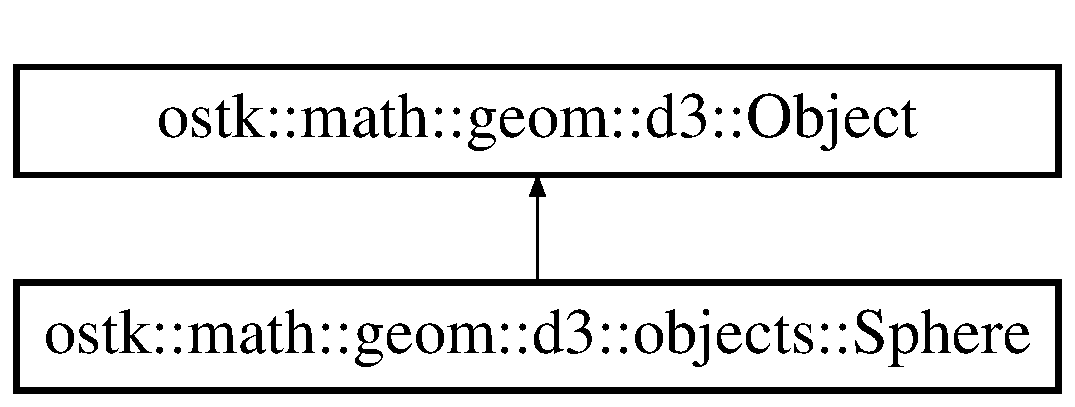
\includegraphics[height=2.000000cm]{classostk_1_1math_1_1geom_1_1d3_1_1objects_1_1_sphere}
\end{center}
\end{figure}
\doxysubsection*{Public Member Functions}
\begin{DoxyCompactItemize}
\item 
\mbox{\hyperlink{classostk_1_1math_1_1geom_1_1d3_1_1objects_1_1_sphere_a6920f72260a7b2c9ffc29283540e16c2}{Sphere}} (const \mbox{\hyperlink{classostk_1_1math_1_1geom_1_1d3_1_1objects_1_1_point}{Point}} \&a\+Center, const Real \&a\+Radius)
\begin{DoxyCompactList}\small\item\em Constructor. \end{DoxyCompactList}\item 
virtual \mbox{\hyperlink{classostk_1_1math_1_1geom_1_1d3_1_1objects_1_1_sphere}{Sphere}} $\ast$ \mbox{\hyperlink{classostk_1_1math_1_1geom_1_1d3_1_1objects_1_1_sphere_a123c8f9f89be73d95db4a0c8dd8c1c7b}{clone}} () const override
\begin{DoxyCompactList}\small\item\em Clone sphere. \end{DoxyCompactList}\item 
bool \mbox{\hyperlink{classostk_1_1math_1_1geom_1_1d3_1_1objects_1_1_sphere_a1bb642dd7e97756a44ca972e6337a43f}{operator==}} (const \mbox{\hyperlink{classostk_1_1math_1_1geom_1_1d3_1_1objects_1_1_sphere}{Sphere}} \&a\+Sphere) const
\begin{DoxyCompactList}\small\item\em Equal to operator. \end{DoxyCompactList}\item 
bool \mbox{\hyperlink{classostk_1_1math_1_1geom_1_1d3_1_1objects_1_1_sphere_ae72e72141c1c4526bfa86161ffb15a37}{operator!=}} (const \mbox{\hyperlink{classostk_1_1math_1_1geom_1_1d3_1_1objects_1_1_sphere}{Sphere}} \&a\+Sphere) const
\begin{DoxyCompactList}\small\item\em Not equal to operator. \end{DoxyCompactList}\item 
virtual bool \mbox{\hyperlink{classostk_1_1math_1_1geom_1_1d3_1_1objects_1_1_sphere_ab236f8c380bcc2164a5a606fdf8bc3a6}{is\+Defined}} () const override
\begin{DoxyCompactList}\small\item\em Check if sphere is defined. \end{DoxyCompactList}\item 
bool \mbox{\hyperlink{classostk_1_1math_1_1geom_1_1d3_1_1objects_1_1_sphere_a9e1c2a66a1d61d461e0e02d5a6cce709}{is\+Unitary}} () const
\begin{DoxyCompactList}\small\item\em Check if sphere is unitary, i.\+e. its radius is equal to 1.\+0. \end{DoxyCompactList}\item 
bool \mbox{\hyperlink{classostk_1_1math_1_1geom_1_1d3_1_1objects_1_1_sphere_a0707e0b1e0e4e382b79ca5bcf643c41c}{intersects}} (const \mbox{\hyperlink{classostk_1_1math_1_1geom_1_1d3_1_1objects_1_1_point}{Point}} \&a\+Point) const
\begin{DoxyCompactList}\small\item\em Check if sphere intersects point. \end{DoxyCompactList}\item 
bool \mbox{\hyperlink{classostk_1_1math_1_1geom_1_1d3_1_1objects_1_1_sphere_a265e91ed533996623854629ac26ee080}{intersects}} (const \mbox{\hyperlink{classostk_1_1math_1_1geom_1_1d3_1_1objects_1_1_point_set}{Point\+Set}} \&a\+Point\+Set) const
\begin{DoxyCompactList}\small\item\em Check if sphere intersects point set. \end{DoxyCompactList}\item 
bool \mbox{\hyperlink{classostk_1_1math_1_1geom_1_1d3_1_1objects_1_1_sphere_a26c5a18cb7543734fb74cad966f512f8}{intersects}} (const \mbox{\hyperlink{classostk_1_1math_1_1geom_1_1d3_1_1objects_1_1_line}{Line}} \&a\+Line) const
\begin{DoxyCompactList}\small\item\em Check if sphere intersects line. \end{DoxyCompactList}\item 
bool \mbox{\hyperlink{classostk_1_1math_1_1geom_1_1d3_1_1objects_1_1_sphere_aff56934077d5851cc168dae45613d78d}{intersects}} (const \mbox{\hyperlink{classostk_1_1math_1_1geom_1_1d3_1_1objects_1_1_ray}{Ray}} \&a\+Ray) const
\begin{DoxyCompactList}\small\item\em Check if sphere intersects ray. \end{DoxyCompactList}\item 
bool \mbox{\hyperlink{classostk_1_1math_1_1geom_1_1d3_1_1objects_1_1_sphere_afccce29f97045441ccc5b6bf37566d18}{intersects}} (const \mbox{\hyperlink{classostk_1_1math_1_1geom_1_1d3_1_1objects_1_1_segment}{Segment}} \&a\+Segment) const
\begin{DoxyCompactList}\small\item\em Check if sphere intersects segment. \end{DoxyCompactList}\item 
bool \mbox{\hyperlink{classostk_1_1math_1_1geom_1_1d3_1_1objects_1_1_sphere_a04479c6d128c10c2395884a82c5abcad}{intersects}} (const \mbox{\hyperlink{classostk_1_1math_1_1geom_1_1d3_1_1objects_1_1_plane}{Plane}} \&a\+Plane) const
\begin{DoxyCompactList}\small\item\em Check if sphere intersects plane. \end{DoxyCompactList}\item 
bool \mbox{\hyperlink{classostk_1_1math_1_1geom_1_1d3_1_1objects_1_1_sphere_acbde8aef7194e50be8be8fe5c5fa2e17}{intersects}} (const \mbox{\hyperlink{classostk_1_1math_1_1geom_1_1d3_1_1objects_1_1_ellipsoid}{Ellipsoid}} \&an\+Ellipsoid) const
\begin{DoxyCompactList}\small\item\em Check if sphere intersects ellipsoid. \end{DoxyCompactList}\item 
bool \mbox{\hyperlink{classostk_1_1math_1_1geom_1_1d3_1_1objects_1_1_sphere_af446f8d8e7dd3fe20a719fe07c2ec91c}{intersects}} (const \mbox{\hyperlink{classostk_1_1math_1_1geom_1_1d3_1_1objects_1_1_pyramid}{Pyramid}} \&a\+Pyramid) const
\begin{DoxyCompactList}\small\item\em Check if sphere intersects pyramid. \end{DoxyCompactList}\item 
bool \mbox{\hyperlink{classostk_1_1math_1_1geom_1_1d3_1_1objects_1_1_sphere_a376f9b54902cab434a6fda22fa40a64e}{intersects}} (const \mbox{\hyperlink{classostk_1_1math_1_1geom_1_1d3_1_1objects_1_1_cone}{Cone}} \&a\+Cone) const
\begin{DoxyCompactList}\small\item\em Check if sphere intersects cone. \end{DoxyCompactList}\item 
bool \mbox{\hyperlink{classostk_1_1math_1_1geom_1_1d3_1_1objects_1_1_sphere_a65299f7b2db42d3ad1b32fc70c9845ae}{contains}} (const \mbox{\hyperlink{classostk_1_1math_1_1geom_1_1d3_1_1objects_1_1_point}{Point}} \&a\+Point) const
\begin{DoxyCompactList}\small\item\em Check if sphere contains point. \end{DoxyCompactList}\item 
bool \mbox{\hyperlink{classostk_1_1math_1_1geom_1_1d3_1_1objects_1_1_sphere_a91a6e5273a96a5bc92da78ea786e2ab5}{contains}} (const \mbox{\hyperlink{classostk_1_1math_1_1geom_1_1d3_1_1objects_1_1_point_set}{Point\+Set}} \&a\+Point\+Set) const
\begin{DoxyCompactList}\small\item\em Check if sphere contains point set. \end{DoxyCompactList}\item 
\mbox{\hyperlink{classostk_1_1math_1_1geom_1_1d3_1_1objects_1_1_point}{Point}} \mbox{\hyperlink{classostk_1_1math_1_1geom_1_1d3_1_1objects_1_1_sphere_aa99591327b0fe9aac8f03dc34b41207a}{get\+Center}} () const
\begin{DoxyCompactList}\small\item\em Get sphere center. \end{DoxyCompactList}\item 
Real \mbox{\hyperlink{classostk_1_1math_1_1geom_1_1d3_1_1objects_1_1_sphere_a856d4bceb6c0e3133aced9eab57d6450}{get\+Radius}} () const
\begin{DoxyCompactList}\small\item\em Get sphere radius. \end{DoxyCompactList}\item 
\mbox{\hyperlink{classostk_1_1math_1_1geom_1_1d3_1_1_intersection}{Intersection}} \mbox{\hyperlink{classostk_1_1math_1_1geom_1_1d3_1_1objects_1_1_sphere_afbae10b116900f5383913e564c0ec91a}{intersection\+With}} (const \mbox{\hyperlink{classostk_1_1math_1_1geom_1_1d3_1_1objects_1_1_line}{Line}} \&a\+Line) const
\begin{DoxyCompactList}\small\item\em Compute intersection of sphere with line. \end{DoxyCompactList}\item 
\mbox{\hyperlink{classostk_1_1math_1_1geom_1_1d3_1_1_intersection}{Intersection}} \mbox{\hyperlink{classostk_1_1math_1_1geom_1_1d3_1_1objects_1_1_sphere_a204e67d24679bed63ab54cafda683918}{intersection\+With}} (const \mbox{\hyperlink{classostk_1_1math_1_1geom_1_1d3_1_1objects_1_1_ray}{Ray}} \&a\+Ray, const bool only\+In\+Sight=\mbox{\hyperlink{_sphere_8hpp_af424617f7c785f4835e2feba5a5640f2}{D\+E\+F\+A\+U\+L\+T\+\_\+\+O\+N\+L\+Y\+\_\+\+I\+N\+\_\+\+S\+I\+G\+HT}}) const
\begin{DoxyCompactList}\small\item\em Compute intersection of sphere with ray. \end{DoxyCompactList}\item 
\mbox{\hyperlink{classostk_1_1math_1_1geom_1_1d3_1_1_intersection}{Intersection}} \mbox{\hyperlink{classostk_1_1math_1_1geom_1_1d3_1_1objects_1_1_sphere_a90b0be4e76f556042518b92fd29f0edf}{intersection\+With}} (const \mbox{\hyperlink{classostk_1_1math_1_1geom_1_1d3_1_1objects_1_1_segment}{Segment}} \&a\+Segment) const
\begin{DoxyCompactList}\small\item\em Compute intersection of sphere with segment. \end{DoxyCompactList}\item 
\mbox{\hyperlink{classostk_1_1math_1_1geom_1_1d3_1_1_intersection}{Intersection}} \mbox{\hyperlink{classostk_1_1math_1_1geom_1_1d3_1_1objects_1_1_sphere_a19df8a41a4853ccf666b8213bed3daf1}{intersection\+With}} (const \mbox{\hyperlink{classostk_1_1math_1_1geom_1_1d3_1_1objects_1_1_pyramid}{Pyramid}} \&a\+Pyramid, const bool only\+In\+Sight=\mbox{\hyperlink{_sphere_8hpp_af424617f7c785f4835e2feba5a5640f2}{D\+E\+F\+A\+U\+L\+T\+\_\+\+O\+N\+L\+Y\+\_\+\+I\+N\+\_\+\+S\+I\+G\+HT}}) const
\begin{DoxyCompactList}\small\item\em Compute intersection of sphere with pyramid. \end{DoxyCompactList}\item 
\mbox{\hyperlink{classostk_1_1math_1_1geom_1_1d3_1_1_intersection}{Intersection}} \mbox{\hyperlink{classostk_1_1math_1_1geom_1_1d3_1_1objects_1_1_sphere_a6a3c2a953d11f6f761207b17e47a6baa}{intersection\+With}} (const \mbox{\hyperlink{classostk_1_1math_1_1geom_1_1d3_1_1objects_1_1_cone}{Cone}} \&a\+Cone, const bool only\+In\+Sight=\mbox{\hyperlink{_sphere_8hpp_af424617f7c785f4835e2feba5a5640f2}{D\+E\+F\+A\+U\+L\+T\+\_\+\+O\+N\+L\+Y\+\_\+\+I\+N\+\_\+\+S\+I\+G\+HT}}) const
\begin{DoxyCompactList}\small\item\em Compute intersection of sphere with cone. \end{DoxyCompactList}\item 
virtual void \mbox{\hyperlink{classostk_1_1math_1_1geom_1_1d3_1_1objects_1_1_sphere_add7bc90c60deddcad6e3486b687a653a}{print}} (std\+::ostream \&an\+Output\+Stream, bool display\+Decorators=true) const override
\begin{DoxyCompactList}\small\item\em Print sphere. \end{DoxyCompactList}\item 
virtual void \mbox{\hyperlink{classostk_1_1math_1_1geom_1_1d3_1_1objects_1_1_sphere_a421357bf4058e68e0aa636f606c6b249}{apply\+Transformation}} (const \mbox{\hyperlink{classostk_1_1math_1_1geom_1_1d3_1_1_transformation}{Transformation}} \&a\+Transformation) override
\begin{DoxyCompactList}\small\item\em Apply transformation to sphere. \end{DoxyCompactList}\end{DoxyCompactItemize}
\doxysubsection*{Static Public Member Functions}
\begin{DoxyCompactItemize}
\item 
static \mbox{\hyperlink{classostk_1_1math_1_1geom_1_1d3_1_1objects_1_1_sphere}{Sphere}} \mbox{\hyperlink{classostk_1_1math_1_1geom_1_1d3_1_1objects_1_1_sphere_ae5092dbaff1a7827de173fd61c8aa0df}{Undefined}} ()
\begin{DoxyCompactList}\small\item\em Constructs an undefined sphere. \end{DoxyCompactList}\item 
static \mbox{\hyperlink{classostk_1_1math_1_1geom_1_1d3_1_1objects_1_1_sphere}{Sphere}} \mbox{\hyperlink{classostk_1_1math_1_1geom_1_1d3_1_1objects_1_1_sphere_a5e0bd57337eb7e5c7eb19b66176d560b}{Unit}} (const \mbox{\hyperlink{classostk_1_1math_1_1geom_1_1d3_1_1objects_1_1_point}{Point}} \&a\+Center)
\begin{DoxyCompactList}\small\item\em Constructs a unit sphere. \end{DoxyCompactList}\end{DoxyCompactItemize}


\doxysubsection{Detailed Description}
\mbox{\hyperlink{classostk_1_1math_1_1geom_1_1d3_1_1objects_1_1_sphere}{Sphere}}. 

\begin{DoxyVerb}                        A sphere is a perfectly round geometrical object in three-dimensional space that is the
                        surface of a completely round ball.
\end{DoxyVerb}


\href{https://en.wikipedia.org/wiki/Sphere}{\texttt{ https\+://en.\+wikipedia.\+org/wiki/\+Sphere}} 

\doxysubsection{Constructor \& Destructor Documentation}
\mbox{\Hypertarget{classostk_1_1math_1_1geom_1_1d3_1_1objects_1_1_sphere_a6920f72260a7b2c9ffc29283540e16c2}\label{classostk_1_1math_1_1geom_1_1d3_1_1objects_1_1_sphere_a6920f72260a7b2c9ffc29283540e16c2}} 
\index{ostk::math::geom::d3::objects::Sphere@{ostk::math::geom::d3::objects::Sphere}!Sphere@{Sphere}}
\index{Sphere@{Sphere}!ostk::math::geom::d3::objects::Sphere@{ostk::math::geom::d3::objects::Sphere}}
\doxysubsubsection{\texorpdfstring{Sphere()}{Sphere()}}
{\footnotesize\ttfamily ostk\+::math\+::geom\+::d3\+::objects\+::\+Sphere\+::\+Sphere (\begin{DoxyParamCaption}\item[{const \mbox{\hyperlink{classostk_1_1math_1_1geom_1_1d3_1_1objects_1_1_point}{Point}} \&}]{a\+Center,  }\item[{const Real \&}]{a\+Radius }\end{DoxyParamCaption})}



Constructor. 


\begin{DoxyCode}{0}
\DoxyCodeLine{\mbox{\hyperlink{classostk_1_1math_1_1geom_1_1d3_1_1objects_1_1_sphere_a6920f72260a7b2c9ffc29283540e16c2}{Sphere}} sphere(\{ 0.0, 0.0, 0.0 \}, 1.0) ;}
\end{DoxyCode}



\begin{DoxyParams}[1]{Parameters}
\mbox{\texttt{ in}}  & {\em a\+Center} & A sphere center \\
\hline
\mbox{\texttt{ in}}  & {\em a\+Radius} & A sphere radius \\
\hline
\end{DoxyParams}


\doxysubsection{Member Function Documentation}
\mbox{\Hypertarget{classostk_1_1math_1_1geom_1_1d3_1_1objects_1_1_sphere_a421357bf4058e68e0aa636f606c6b249}\label{classostk_1_1math_1_1geom_1_1d3_1_1objects_1_1_sphere_a421357bf4058e68e0aa636f606c6b249}} 
\index{ostk::math::geom::d3::objects::Sphere@{ostk::math::geom::d3::objects::Sphere}!applyTransformation@{applyTransformation}}
\index{applyTransformation@{applyTransformation}!ostk::math::geom::d3::objects::Sphere@{ostk::math::geom::d3::objects::Sphere}}
\doxysubsubsection{\texorpdfstring{applyTransformation()}{applyTransformation()}}
{\footnotesize\ttfamily void ostk\+::math\+::geom\+::d3\+::objects\+::\+Sphere\+::apply\+Transformation (\begin{DoxyParamCaption}\item[{const \mbox{\hyperlink{classostk_1_1math_1_1geom_1_1d3_1_1_transformation}{Transformation}} \&}]{a\+Transformation }\end{DoxyParamCaption})\hspace{0.3cm}{\ttfamily [override]}, {\ttfamily [virtual]}}



Apply transformation to sphere. 


\begin{DoxyParams}[1]{Parameters}
\mbox{\texttt{ in}}  & {\em a\+Transformation} & A transformation \\
\hline
\end{DoxyParams}


Implements \mbox{\hyperlink{classostk_1_1math_1_1geom_1_1d3_1_1_object_ae9194dd6d2bb4df09292ffc84dccdb1d}{ostk\+::math\+::geom\+::d3\+::\+Object}}.

\mbox{\Hypertarget{classostk_1_1math_1_1geom_1_1d3_1_1objects_1_1_sphere_a123c8f9f89be73d95db4a0c8dd8c1c7b}\label{classostk_1_1math_1_1geom_1_1d3_1_1objects_1_1_sphere_a123c8f9f89be73d95db4a0c8dd8c1c7b}} 
\index{ostk::math::geom::d3::objects::Sphere@{ostk::math::geom::d3::objects::Sphere}!clone@{clone}}
\index{clone@{clone}!ostk::math::geom::d3::objects::Sphere@{ostk::math::geom::d3::objects::Sphere}}
\doxysubsubsection{\texorpdfstring{clone()}{clone()}}
{\footnotesize\ttfamily \mbox{\hyperlink{classostk_1_1math_1_1geom_1_1d3_1_1objects_1_1_sphere}{Sphere}} $\ast$ ostk\+::math\+::geom\+::d3\+::objects\+::\+Sphere\+::clone (\begin{DoxyParamCaption}{ }\end{DoxyParamCaption}) const\hspace{0.3cm}{\ttfamily [override]}, {\ttfamily [virtual]}}



Clone sphere. 

\begin{DoxyReturn}{Returns}
Pointer to cloned sphere 
\end{DoxyReturn}


Implements \mbox{\hyperlink{classostk_1_1math_1_1geom_1_1d3_1_1_object_a676013f9555f6492687f9809b2db887b}{ostk\+::math\+::geom\+::d3\+::\+Object}}.

\mbox{\Hypertarget{classostk_1_1math_1_1geom_1_1d3_1_1objects_1_1_sphere_a65299f7b2db42d3ad1b32fc70c9845ae}\label{classostk_1_1math_1_1geom_1_1d3_1_1objects_1_1_sphere_a65299f7b2db42d3ad1b32fc70c9845ae}} 
\index{ostk::math::geom::d3::objects::Sphere@{ostk::math::geom::d3::objects::Sphere}!contains@{contains}}
\index{contains@{contains}!ostk::math::geom::d3::objects::Sphere@{ostk::math::geom::d3::objects::Sphere}}
\doxysubsubsection{\texorpdfstring{contains()}{contains()}\hspace{0.1cm}{\footnotesize\ttfamily [1/2]}}
{\footnotesize\ttfamily bool ostk\+::math\+::geom\+::d3\+::objects\+::\+Sphere\+::contains (\begin{DoxyParamCaption}\item[{const \mbox{\hyperlink{classostk_1_1math_1_1geom_1_1d3_1_1objects_1_1_point}{Point}} \&}]{a\+Point }\end{DoxyParamCaption}) const}



Check if sphere contains point. 


\begin{DoxyCode}{0}
\DoxyCodeLine{\mbox{\hyperlink{classostk_1_1math_1_1geom_1_1d3_1_1objects_1_1_sphere_a6920f72260a7b2c9ffc29283540e16c2}{Sphere}} sphere = ... ;}
\DoxyCodeLine{Point point = ... ;}
\DoxyCodeLine{sphere.contains(point) ;}
\end{DoxyCode}



\begin{DoxyParams}[1]{Parameters}
\mbox{\texttt{ in}}  & {\em a\+Point} & A point \\
\hline
\end{DoxyParams}
\begin{DoxyReturn}{Returns}
True if sphere contains point 
\end{DoxyReturn}
\mbox{\Hypertarget{classostk_1_1math_1_1geom_1_1d3_1_1objects_1_1_sphere_a91a6e5273a96a5bc92da78ea786e2ab5}\label{classostk_1_1math_1_1geom_1_1d3_1_1objects_1_1_sphere_a91a6e5273a96a5bc92da78ea786e2ab5}} 
\index{ostk::math::geom::d3::objects::Sphere@{ostk::math::geom::d3::objects::Sphere}!contains@{contains}}
\index{contains@{contains}!ostk::math::geom::d3::objects::Sphere@{ostk::math::geom::d3::objects::Sphere}}
\doxysubsubsection{\texorpdfstring{contains()}{contains()}\hspace{0.1cm}{\footnotesize\ttfamily [2/2]}}
{\footnotesize\ttfamily bool ostk\+::math\+::geom\+::d3\+::objects\+::\+Sphere\+::contains (\begin{DoxyParamCaption}\item[{const \mbox{\hyperlink{classostk_1_1math_1_1geom_1_1d3_1_1objects_1_1_point_set}{Point\+Set}} \&}]{a\+Point\+Set }\end{DoxyParamCaption}) const}



Check if sphere contains point set. 


\begin{DoxyCode}{0}
\DoxyCodeLine{\mbox{\hyperlink{classostk_1_1math_1_1geom_1_1d3_1_1objects_1_1_sphere_a6920f72260a7b2c9ffc29283540e16c2}{Sphere}} sphere = ... ;}
\DoxyCodeLine{PointSet pointSet = ... ;}
\DoxyCodeLine{sphere.contains(pointSet) ;}
\end{DoxyCode}



\begin{DoxyParams}[1]{Parameters}
\mbox{\texttt{ in}}  & {\em a\+Point\+Set} & A point set \\
\hline
\end{DoxyParams}
\begin{DoxyReturn}{Returns}
True if sphere contains point set 
\end{DoxyReturn}
\mbox{\Hypertarget{classostk_1_1math_1_1geom_1_1d3_1_1objects_1_1_sphere_aa99591327b0fe9aac8f03dc34b41207a}\label{classostk_1_1math_1_1geom_1_1d3_1_1objects_1_1_sphere_aa99591327b0fe9aac8f03dc34b41207a}} 
\index{ostk::math::geom::d3::objects::Sphere@{ostk::math::geom::d3::objects::Sphere}!getCenter@{getCenter}}
\index{getCenter@{getCenter}!ostk::math::geom::d3::objects::Sphere@{ostk::math::geom::d3::objects::Sphere}}
\doxysubsubsection{\texorpdfstring{getCenter()}{getCenter()}}
{\footnotesize\ttfamily \mbox{\hyperlink{classostk_1_1math_1_1geom_1_1d3_1_1objects_1_1_point}{Point}} ostk\+::math\+::geom\+::d3\+::objects\+::\+Sphere\+::get\+Center (\begin{DoxyParamCaption}{ }\end{DoxyParamCaption}) const}



Get sphere center. 


\begin{DoxyCode}{0}
\DoxyCodeLine{\mbox{\hyperlink{classostk_1_1math_1_1geom_1_1d3_1_1objects_1_1_sphere_a6920f72260a7b2c9ffc29283540e16c2}{Sphere}}(\mbox{\hyperlink{classostk_1_1math_1_1geom_1_1d3_1_1objects_1_1_point_a079c199f08b015d456d02728a71b534c}{Point::Origin}}(), 1.0).getCenter() ; \textcolor{comment}{// [0.0, 0.0, 0.0]}}
\end{DoxyCode}


\begin{DoxyReturn}{Returns}
\mbox{\hyperlink{classostk_1_1math_1_1geom_1_1d3_1_1objects_1_1_sphere}{Sphere}} center 
\end{DoxyReturn}
\mbox{\Hypertarget{classostk_1_1math_1_1geom_1_1d3_1_1objects_1_1_sphere_a856d4bceb6c0e3133aced9eab57d6450}\label{classostk_1_1math_1_1geom_1_1d3_1_1objects_1_1_sphere_a856d4bceb6c0e3133aced9eab57d6450}} 
\index{ostk::math::geom::d3::objects::Sphere@{ostk::math::geom::d3::objects::Sphere}!getRadius@{getRadius}}
\index{getRadius@{getRadius}!ostk::math::geom::d3::objects::Sphere@{ostk::math::geom::d3::objects::Sphere}}
\doxysubsubsection{\texorpdfstring{getRadius()}{getRadius()}}
{\footnotesize\ttfamily Real ostk\+::math\+::geom\+::d3\+::objects\+::\+Sphere\+::get\+Radius (\begin{DoxyParamCaption}{ }\end{DoxyParamCaption}) const}



Get sphere radius. 


\begin{DoxyCode}{0}
\DoxyCodeLine{\mbox{\hyperlink{classostk_1_1math_1_1geom_1_1d3_1_1objects_1_1_sphere_a6920f72260a7b2c9ffc29283540e16c2}{Sphere}}(\mbox{\hyperlink{classostk_1_1math_1_1geom_1_1d3_1_1objects_1_1_point_a079c199f08b015d456d02728a71b534c}{Point::Origin}}(), 1.0).getRadius() ; \textcolor{comment}{// 1.0}}
\end{DoxyCode}


\begin{DoxyReturn}{Returns}
\mbox{\hyperlink{classostk_1_1math_1_1geom_1_1d3_1_1objects_1_1_sphere}{Sphere}} radius 
\end{DoxyReturn}
\mbox{\Hypertarget{classostk_1_1math_1_1geom_1_1d3_1_1objects_1_1_sphere_a6a3c2a953d11f6f761207b17e47a6baa}\label{classostk_1_1math_1_1geom_1_1d3_1_1objects_1_1_sphere_a6a3c2a953d11f6f761207b17e47a6baa}} 
\index{ostk::math::geom::d3::objects::Sphere@{ostk::math::geom::d3::objects::Sphere}!intersectionWith@{intersectionWith}}
\index{intersectionWith@{intersectionWith}!ostk::math::geom::d3::objects::Sphere@{ostk::math::geom::d3::objects::Sphere}}
\doxysubsubsection{\texorpdfstring{intersectionWith()}{intersectionWith()}\hspace{0.1cm}{\footnotesize\ttfamily [1/5]}}
{\footnotesize\ttfamily \mbox{\hyperlink{classostk_1_1math_1_1geom_1_1d3_1_1_intersection}{Intersection}} ostk\+::math\+::geom\+::d3\+::objects\+::\+Sphere\+::intersection\+With (\begin{DoxyParamCaption}\item[{const \mbox{\hyperlink{classostk_1_1math_1_1geom_1_1d3_1_1objects_1_1_cone}{Cone}} \&}]{a\+Cone,  }\item[{const bool}]{only\+In\+Sight = {\ttfamily \mbox{\hyperlink{_sphere_8hpp_af424617f7c785f4835e2feba5a5640f2}{D\+E\+F\+A\+U\+L\+T\+\_\+\+O\+N\+L\+Y\+\_\+\+I\+N\+\_\+\+S\+I\+G\+HT}}} }\end{DoxyParamCaption}) const}



Compute intersection of sphere with cone. 


\begin{DoxyParams}[1]{Parameters}
\mbox{\texttt{ in}}  & {\em a\+Cone} & A cone \\
\hline
\mbox{\texttt{ in}}  & {\em only\+In\+Sight} & (optional) If true, only return intersection points that are in sight \\
\hline
\end{DoxyParams}
\begin{DoxyReturn}{Returns}
\mbox{\hyperlink{classostk_1_1math_1_1geom_1_1d3_1_1_intersection}{Intersection}} of sphere with cone 
\end{DoxyReturn}
\mbox{\Hypertarget{classostk_1_1math_1_1geom_1_1d3_1_1objects_1_1_sphere_afbae10b116900f5383913e564c0ec91a}\label{classostk_1_1math_1_1geom_1_1d3_1_1objects_1_1_sphere_afbae10b116900f5383913e564c0ec91a}} 
\index{ostk::math::geom::d3::objects::Sphere@{ostk::math::geom::d3::objects::Sphere}!intersectionWith@{intersectionWith}}
\index{intersectionWith@{intersectionWith}!ostk::math::geom::d3::objects::Sphere@{ostk::math::geom::d3::objects::Sphere}}
\doxysubsubsection{\texorpdfstring{intersectionWith()}{intersectionWith()}\hspace{0.1cm}{\footnotesize\ttfamily [2/5]}}
{\footnotesize\ttfamily \mbox{\hyperlink{classostk_1_1math_1_1geom_1_1d3_1_1_intersection}{Intersection}} ostk\+::math\+::geom\+::d3\+::objects\+::\+Sphere\+::intersection\+With (\begin{DoxyParamCaption}\item[{const \mbox{\hyperlink{classostk_1_1math_1_1geom_1_1d3_1_1objects_1_1_line}{Line}} \&}]{a\+Line }\end{DoxyParamCaption}) const}



Compute intersection of sphere with line. 


\begin{DoxyParams}[1]{Parameters}
\mbox{\texttt{ in}}  & {\em a\+Line} & A line \\
\hline
\end{DoxyParams}
\begin{DoxyReturn}{Returns}
\mbox{\hyperlink{classostk_1_1math_1_1geom_1_1d3_1_1_intersection}{Intersection}} of sphere with line 
\end{DoxyReturn}
\mbox{\Hypertarget{classostk_1_1math_1_1geom_1_1d3_1_1objects_1_1_sphere_a19df8a41a4853ccf666b8213bed3daf1}\label{classostk_1_1math_1_1geom_1_1d3_1_1objects_1_1_sphere_a19df8a41a4853ccf666b8213bed3daf1}} 
\index{ostk::math::geom::d3::objects::Sphere@{ostk::math::geom::d3::objects::Sphere}!intersectionWith@{intersectionWith}}
\index{intersectionWith@{intersectionWith}!ostk::math::geom::d3::objects::Sphere@{ostk::math::geom::d3::objects::Sphere}}
\doxysubsubsection{\texorpdfstring{intersectionWith()}{intersectionWith()}\hspace{0.1cm}{\footnotesize\ttfamily [3/5]}}
{\footnotesize\ttfamily \mbox{\hyperlink{classostk_1_1math_1_1geom_1_1d3_1_1_intersection}{Intersection}} ostk\+::math\+::geom\+::d3\+::objects\+::\+Sphere\+::intersection\+With (\begin{DoxyParamCaption}\item[{const \mbox{\hyperlink{classostk_1_1math_1_1geom_1_1d3_1_1objects_1_1_pyramid}{Pyramid}} \&}]{a\+Pyramid,  }\item[{const bool}]{only\+In\+Sight = {\ttfamily \mbox{\hyperlink{_sphere_8hpp_af424617f7c785f4835e2feba5a5640f2}{D\+E\+F\+A\+U\+L\+T\+\_\+\+O\+N\+L\+Y\+\_\+\+I\+N\+\_\+\+S\+I\+G\+HT}}} }\end{DoxyParamCaption}) const}



Compute intersection of sphere with pyramid. 


\begin{DoxyParams}[1]{Parameters}
\mbox{\texttt{ in}}  & {\em a\+Pyramid} & A pyramid \\
\hline
\mbox{\texttt{ in}}  & {\em only\+In\+Sight} & (optional) If true, only return intersection points that are in sight \\
\hline
\end{DoxyParams}
\begin{DoxyReturn}{Returns}
\mbox{\hyperlink{classostk_1_1math_1_1geom_1_1d3_1_1_intersection}{Intersection}} of sphere with pyramid 
\end{DoxyReturn}
\mbox{\Hypertarget{classostk_1_1math_1_1geom_1_1d3_1_1objects_1_1_sphere_a204e67d24679bed63ab54cafda683918}\label{classostk_1_1math_1_1geom_1_1d3_1_1objects_1_1_sphere_a204e67d24679bed63ab54cafda683918}} 
\index{ostk::math::geom::d3::objects::Sphere@{ostk::math::geom::d3::objects::Sphere}!intersectionWith@{intersectionWith}}
\index{intersectionWith@{intersectionWith}!ostk::math::geom::d3::objects::Sphere@{ostk::math::geom::d3::objects::Sphere}}
\doxysubsubsection{\texorpdfstring{intersectionWith()}{intersectionWith()}\hspace{0.1cm}{\footnotesize\ttfamily [4/5]}}
{\footnotesize\ttfamily \mbox{\hyperlink{classostk_1_1math_1_1geom_1_1d3_1_1_intersection}{Intersection}} ostk\+::math\+::geom\+::d3\+::objects\+::\+Sphere\+::intersection\+With (\begin{DoxyParamCaption}\item[{const \mbox{\hyperlink{classostk_1_1math_1_1geom_1_1d3_1_1objects_1_1_ray}{Ray}} \&}]{a\+Ray,  }\item[{const bool}]{only\+In\+Sight = {\ttfamily \mbox{\hyperlink{_sphere_8hpp_af424617f7c785f4835e2feba5a5640f2}{D\+E\+F\+A\+U\+L\+T\+\_\+\+O\+N\+L\+Y\+\_\+\+I\+N\+\_\+\+S\+I\+G\+HT}}} }\end{DoxyParamCaption}) const}



Compute intersection of sphere with ray. 


\begin{DoxyParams}[1]{Parameters}
\mbox{\texttt{ in}}  & {\em a\+Ray} & A ray \\
\hline
\mbox{\texttt{ in}}  & {\em only\+In\+Sight} & (optional) If true, only return intersection points that are in sight \\
\hline
\end{DoxyParams}
\begin{DoxyReturn}{Returns}
\mbox{\hyperlink{classostk_1_1math_1_1geom_1_1d3_1_1_intersection}{Intersection}} of sphere with ray 
\end{DoxyReturn}
\mbox{\Hypertarget{classostk_1_1math_1_1geom_1_1d3_1_1objects_1_1_sphere_a90b0be4e76f556042518b92fd29f0edf}\label{classostk_1_1math_1_1geom_1_1d3_1_1objects_1_1_sphere_a90b0be4e76f556042518b92fd29f0edf}} 
\index{ostk::math::geom::d3::objects::Sphere@{ostk::math::geom::d3::objects::Sphere}!intersectionWith@{intersectionWith}}
\index{intersectionWith@{intersectionWith}!ostk::math::geom::d3::objects::Sphere@{ostk::math::geom::d3::objects::Sphere}}
\doxysubsubsection{\texorpdfstring{intersectionWith()}{intersectionWith()}\hspace{0.1cm}{\footnotesize\ttfamily [5/5]}}
{\footnotesize\ttfamily \mbox{\hyperlink{classostk_1_1math_1_1geom_1_1d3_1_1_intersection}{Intersection}} ostk\+::math\+::geom\+::d3\+::objects\+::\+Sphere\+::intersection\+With (\begin{DoxyParamCaption}\item[{const \mbox{\hyperlink{classostk_1_1math_1_1geom_1_1d3_1_1objects_1_1_segment}{Segment}} \&}]{a\+Segment }\end{DoxyParamCaption}) const}



Compute intersection of sphere with segment. 


\begin{DoxyParams}[1]{Parameters}
\mbox{\texttt{ in}}  & {\em a\+Segment} & A segment \\
\hline
\end{DoxyParams}
\begin{DoxyReturn}{Returns}
\mbox{\hyperlink{classostk_1_1math_1_1geom_1_1d3_1_1_intersection}{Intersection}} of sphere with segment 
\end{DoxyReturn}
\mbox{\Hypertarget{classostk_1_1math_1_1geom_1_1d3_1_1objects_1_1_sphere_a376f9b54902cab434a6fda22fa40a64e}\label{classostk_1_1math_1_1geom_1_1d3_1_1objects_1_1_sphere_a376f9b54902cab434a6fda22fa40a64e}} 
\index{ostk::math::geom::d3::objects::Sphere@{ostk::math::geom::d3::objects::Sphere}!intersects@{intersects}}
\index{intersects@{intersects}!ostk::math::geom::d3::objects::Sphere@{ostk::math::geom::d3::objects::Sphere}}
\doxysubsubsection{\texorpdfstring{intersects()}{intersects()}\hspace{0.1cm}{\footnotesize\ttfamily [1/9]}}
{\footnotesize\ttfamily bool ostk\+::math\+::geom\+::d3\+::objects\+::\+Sphere\+::intersects (\begin{DoxyParamCaption}\item[{const \mbox{\hyperlink{classostk_1_1math_1_1geom_1_1d3_1_1objects_1_1_cone}{Cone}} \&}]{a\+Cone }\end{DoxyParamCaption}) const}



Check if sphere intersects cone. 


\begin{DoxyCode}{0}
\DoxyCodeLine{\mbox{\hyperlink{classostk_1_1math_1_1geom_1_1d3_1_1objects_1_1_sphere_a6920f72260a7b2c9ffc29283540e16c2}{Sphere}} sphere = ... ;}
\DoxyCodeLine{Cone cone = ... ;}
\DoxyCodeLine{sphere.intersects(cone) ;}
\end{DoxyCode}



\begin{DoxyParams}[1]{Parameters}
\mbox{\texttt{ in}}  & {\em a\+Cone} & A cone \\
\hline
\end{DoxyParams}
\begin{DoxyReturn}{Returns}
True if sphere intersects cone 
\end{DoxyReturn}
\mbox{\Hypertarget{classostk_1_1math_1_1geom_1_1d3_1_1objects_1_1_sphere_acbde8aef7194e50be8be8fe5c5fa2e17}\label{classostk_1_1math_1_1geom_1_1d3_1_1objects_1_1_sphere_acbde8aef7194e50be8be8fe5c5fa2e17}} 
\index{ostk::math::geom::d3::objects::Sphere@{ostk::math::geom::d3::objects::Sphere}!intersects@{intersects}}
\index{intersects@{intersects}!ostk::math::geom::d3::objects::Sphere@{ostk::math::geom::d3::objects::Sphere}}
\doxysubsubsection{\texorpdfstring{intersects()}{intersects()}\hspace{0.1cm}{\footnotesize\ttfamily [2/9]}}
{\footnotesize\ttfamily bool ostk\+::math\+::geom\+::d3\+::objects\+::\+Sphere\+::intersects (\begin{DoxyParamCaption}\item[{const \mbox{\hyperlink{classostk_1_1math_1_1geom_1_1d3_1_1objects_1_1_ellipsoid}{Ellipsoid}} \&}]{an\+Ellipsoid }\end{DoxyParamCaption}) const}



Check if sphere intersects ellipsoid. 


\begin{DoxyCode}{0}
\DoxyCodeLine{\mbox{\hyperlink{classostk_1_1math_1_1geom_1_1d3_1_1objects_1_1_sphere_a6920f72260a7b2c9ffc29283540e16c2}{Sphere}} sphere = ... ;}
\DoxyCodeLine{Ellipsoid ellipsoid = ... ;}
\DoxyCodeLine{sphere.intersects(ellipsoid) ;}
\end{DoxyCode}



\begin{DoxyParams}[1]{Parameters}
\mbox{\texttt{ in}}  & {\em an\+Ellipsoid} & An ellipsoid \\
\hline
\end{DoxyParams}
\begin{DoxyReturn}{Returns}
True if sphere intersects ellipsoid 
\end{DoxyReturn}
\mbox{\Hypertarget{classostk_1_1math_1_1geom_1_1d3_1_1objects_1_1_sphere_a26c5a18cb7543734fb74cad966f512f8}\label{classostk_1_1math_1_1geom_1_1d3_1_1objects_1_1_sphere_a26c5a18cb7543734fb74cad966f512f8}} 
\index{ostk::math::geom::d3::objects::Sphere@{ostk::math::geom::d3::objects::Sphere}!intersects@{intersects}}
\index{intersects@{intersects}!ostk::math::geom::d3::objects::Sphere@{ostk::math::geom::d3::objects::Sphere}}
\doxysubsubsection{\texorpdfstring{intersects()}{intersects()}\hspace{0.1cm}{\footnotesize\ttfamily [3/9]}}
{\footnotesize\ttfamily bool ostk\+::math\+::geom\+::d3\+::objects\+::\+Sphere\+::intersects (\begin{DoxyParamCaption}\item[{const \mbox{\hyperlink{classostk_1_1math_1_1geom_1_1d3_1_1objects_1_1_line}{Line}} \&}]{a\+Line }\end{DoxyParamCaption}) const}



Check if sphere intersects line. 


\begin{DoxyCode}{0}
\DoxyCodeLine{\mbox{\hyperlink{classostk_1_1math_1_1geom_1_1d3_1_1objects_1_1_sphere_a6920f72260a7b2c9ffc29283540e16c2}{Sphere}} sphere = ... ;}
\DoxyCodeLine{Line line = ... ;}
\DoxyCodeLine{sphere.intersects(line) ;}
\end{DoxyCode}



\begin{DoxyParams}[1]{Parameters}
\mbox{\texttt{ in}}  & {\em a\+Line} & A line \\
\hline
\end{DoxyParams}
\begin{DoxyReturn}{Returns}
True if sphere intersects line 
\end{DoxyReturn}
\mbox{\Hypertarget{classostk_1_1math_1_1geom_1_1d3_1_1objects_1_1_sphere_a04479c6d128c10c2395884a82c5abcad}\label{classostk_1_1math_1_1geom_1_1d3_1_1objects_1_1_sphere_a04479c6d128c10c2395884a82c5abcad}} 
\index{ostk::math::geom::d3::objects::Sphere@{ostk::math::geom::d3::objects::Sphere}!intersects@{intersects}}
\index{intersects@{intersects}!ostk::math::geom::d3::objects::Sphere@{ostk::math::geom::d3::objects::Sphere}}
\doxysubsubsection{\texorpdfstring{intersects()}{intersects()}\hspace{0.1cm}{\footnotesize\ttfamily [4/9]}}
{\footnotesize\ttfamily bool ostk\+::math\+::geom\+::d3\+::objects\+::\+Sphere\+::intersects (\begin{DoxyParamCaption}\item[{const \mbox{\hyperlink{classostk_1_1math_1_1geom_1_1d3_1_1objects_1_1_plane}{Plane}} \&}]{a\+Plane }\end{DoxyParamCaption}) const}



Check if sphere intersects plane. 


\begin{DoxyCode}{0}
\DoxyCodeLine{\mbox{\hyperlink{classostk_1_1math_1_1geom_1_1d3_1_1objects_1_1_sphere_a6920f72260a7b2c9ffc29283540e16c2}{Sphere}} sphere = ... ;}
\DoxyCodeLine{Plane plane = ... ;}
\DoxyCodeLine{sphere.intersects(plane) ;}
\end{DoxyCode}



\begin{DoxyParams}[1]{Parameters}
\mbox{\texttt{ in}}  & {\em a\+Plane} & A plane \\
\hline
\end{DoxyParams}
\begin{DoxyReturn}{Returns}
True if sphere intersects plane 
\end{DoxyReturn}
\mbox{\Hypertarget{classostk_1_1math_1_1geom_1_1d3_1_1objects_1_1_sphere_a0707e0b1e0e4e382b79ca5bcf643c41c}\label{classostk_1_1math_1_1geom_1_1d3_1_1objects_1_1_sphere_a0707e0b1e0e4e382b79ca5bcf643c41c}} 
\index{ostk::math::geom::d3::objects::Sphere@{ostk::math::geom::d3::objects::Sphere}!intersects@{intersects}}
\index{intersects@{intersects}!ostk::math::geom::d3::objects::Sphere@{ostk::math::geom::d3::objects::Sphere}}
\doxysubsubsection{\texorpdfstring{intersects()}{intersects()}\hspace{0.1cm}{\footnotesize\ttfamily [5/9]}}
{\footnotesize\ttfamily bool ostk\+::math\+::geom\+::d3\+::objects\+::\+Sphere\+::intersects (\begin{DoxyParamCaption}\item[{const \mbox{\hyperlink{classostk_1_1math_1_1geom_1_1d3_1_1objects_1_1_point}{Point}} \&}]{a\+Point }\end{DoxyParamCaption}) const}



Check if sphere intersects point. 


\begin{DoxyCode}{0}
\DoxyCodeLine{\mbox{\hyperlink{classostk_1_1math_1_1geom_1_1d3_1_1objects_1_1_sphere_a6920f72260a7b2c9ffc29283540e16c2}{Sphere}} sphere = ... ;}
\DoxyCodeLine{Point point = ... ;}
\DoxyCodeLine{sphere.intersects(point) ;}
\end{DoxyCode}



\begin{DoxyParams}[1]{Parameters}
\mbox{\texttt{ in}}  & {\em a\+Point} & A point \\
\hline
\end{DoxyParams}
\begin{DoxyReturn}{Returns}
True if sphere intersects point 
\end{DoxyReturn}
\mbox{\Hypertarget{classostk_1_1math_1_1geom_1_1d3_1_1objects_1_1_sphere_a265e91ed533996623854629ac26ee080}\label{classostk_1_1math_1_1geom_1_1d3_1_1objects_1_1_sphere_a265e91ed533996623854629ac26ee080}} 
\index{ostk::math::geom::d3::objects::Sphere@{ostk::math::geom::d3::objects::Sphere}!intersects@{intersects}}
\index{intersects@{intersects}!ostk::math::geom::d3::objects::Sphere@{ostk::math::geom::d3::objects::Sphere}}
\doxysubsubsection{\texorpdfstring{intersects()}{intersects()}\hspace{0.1cm}{\footnotesize\ttfamily [6/9]}}
{\footnotesize\ttfamily bool ostk\+::math\+::geom\+::d3\+::objects\+::\+Sphere\+::intersects (\begin{DoxyParamCaption}\item[{const \mbox{\hyperlink{classostk_1_1math_1_1geom_1_1d3_1_1objects_1_1_point_set}{Point\+Set}} \&}]{a\+Point\+Set }\end{DoxyParamCaption}) const}



Check if sphere intersects point set. 


\begin{DoxyCode}{0}
\DoxyCodeLine{\mbox{\hyperlink{classostk_1_1math_1_1geom_1_1d3_1_1objects_1_1_sphere_a6920f72260a7b2c9ffc29283540e16c2}{Sphere}} sphere = ... ;}
\DoxyCodeLine{PointSet pointSet = ... ;}
\DoxyCodeLine{sphere.intersects(pointSet) ;}
\end{DoxyCode}



\begin{DoxyParams}[1]{Parameters}
\mbox{\texttt{ in}}  & {\em a\+Point\+Set} & A point set \\
\hline
\end{DoxyParams}
\begin{DoxyReturn}{Returns}
True if sphere intersects point set 
\end{DoxyReturn}
\mbox{\Hypertarget{classostk_1_1math_1_1geom_1_1d3_1_1objects_1_1_sphere_af446f8d8e7dd3fe20a719fe07c2ec91c}\label{classostk_1_1math_1_1geom_1_1d3_1_1objects_1_1_sphere_af446f8d8e7dd3fe20a719fe07c2ec91c}} 
\index{ostk::math::geom::d3::objects::Sphere@{ostk::math::geom::d3::objects::Sphere}!intersects@{intersects}}
\index{intersects@{intersects}!ostk::math::geom::d3::objects::Sphere@{ostk::math::geom::d3::objects::Sphere}}
\doxysubsubsection{\texorpdfstring{intersects()}{intersects()}\hspace{0.1cm}{\footnotesize\ttfamily [7/9]}}
{\footnotesize\ttfamily bool ostk\+::math\+::geom\+::d3\+::objects\+::\+Sphere\+::intersects (\begin{DoxyParamCaption}\item[{const \mbox{\hyperlink{classostk_1_1math_1_1geom_1_1d3_1_1objects_1_1_pyramid}{Pyramid}} \&}]{a\+Pyramid }\end{DoxyParamCaption}) const}



Check if sphere intersects pyramid. 


\begin{DoxyCode}{0}
\DoxyCodeLine{\mbox{\hyperlink{classostk_1_1math_1_1geom_1_1d3_1_1objects_1_1_sphere_a6920f72260a7b2c9ffc29283540e16c2}{Sphere}} sphere = ... ;}
\DoxyCodeLine{Pyramid pyramid = ... ;}
\DoxyCodeLine{sphere.intersects(pyramid) ;}
\end{DoxyCode}



\begin{DoxyParams}[1]{Parameters}
\mbox{\texttt{ in}}  & {\em a\+Pyramid} & A pyramid \\
\hline
\end{DoxyParams}
\begin{DoxyReturn}{Returns}
True if sphere intersects pyramid 
\end{DoxyReturn}
\mbox{\Hypertarget{classostk_1_1math_1_1geom_1_1d3_1_1objects_1_1_sphere_aff56934077d5851cc168dae45613d78d}\label{classostk_1_1math_1_1geom_1_1d3_1_1objects_1_1_sphere_aff56934077d5851cc168dae45613d78d}} 
\index{ostk::math::geom::d3::objects::Sphere@{ostk::math::geom::d3::objects::Sphere}!intersects@{intersects}}
\index{intersects@{intersects}!ostk::math::geom::d3::objects::Sphere@{ostk::math::geom::d3::objects::Sphere}}
\doxysubsubsection{\texorpdfstring{intersects()}{intersects()}\hspace{0.1cm}{\footnotesize\ttfamily [8/9]}}
{\footnotesize\ttfamily bool ostk\+::math\+::geom\+::d3\+::objects\+::\+Sphere\+::intersects (\begin{DoxyParamCaption}\item[{const \mbox{\hyperlink{classostk_1_1math_1_1geom_1_1d3_1_1objects_1_1_ray}{Ray}} \&}]{a\+Ray }\end{DoxyParamCaption}) const}



Check if sphere intersects ray. 


\begin{DoxyCode}{0}
\DoxyCodeLine{\mbox{\hyperlink{classostk_1_1math_1_1geom_1_1d3_1_1objects_1_1_sphere_a6920f72260a7b2c9ffc29283540e16c2}{Sphere}} sphere = ... ;}
\DoxyCodeLine{Ray ray = ... ;}
\DoxyCodeLine{sphere.intersects(ray) ;}
\end{DoxyCode}



\begin{DoxyParams}[1]{Parameters}
\mbox{\texttt{ in}}  & {\em a\+Ray} & A ray \\
\hline
\end{DoxyParams}
\begin{DoxyReturn}{Returns}
True if sphere intersects ray 
\end{DoxyReturn}
\mbox{\Hypertarget{classostk_1_1math_1_1geom_1_1d3_1_1objects_1_1_sphere_afccce29f97045441ccc5b6bf37566d18}\label{classostk_1_1math_1_1geom_1_1d3_1_1objects_1_1_sphere_afccce29f97045441ccc5b6bf37566d18}} 
\index{ostk::math::geom::d3::objects::Sphere@{ostk::math::geom::d3::objects::Sphere}!intersects@{intersects}}
\index{intersects@{intersects}!ostk::math::geom::d3::objects::Sphere@{ostk::math::geom::d3::objects::Sphere}}
\doxysubsubsection{\texorpdfstring{intersects()}{intersects()}\hspace{0.1cm}{\footnotesize\ttfamily [9/9]}}
{\footnotesize\ttfamily bool ostk\+::math\+::geom\+::d3\+::objects\+::\+Sphere\+::intersects (\begin{DoxyParamCaption}\item[{const \mbox{\hyperlink{classostk_1_1math_1_1geom_1_1d3_1_1objects_1_1_segment}{Segment}} \&}]{a\+Segment }\end{DoxyParamCaption}) const}



Check if sphere intersects segment. 


\begin{DoxyCode}{0}
\DoxyCodeLine{\mbox{\hyperlink{classostk_1_1math_1_1geom_1_1d3_1_1objects_1_1_sphere_a6920f72260a7b2c9ffc29283540e16c2}{Sphere}} sphere = ... ;}
\DoxyCodeLine{Segment segment = ... ;}
\DoxyCodeLine{sphere.intersects(segment) ;}
\end{DoxyCode}



\begin{DoxyParams}[1]{Parameters}
\mbox{\texttt{ in}}  & {\em a\+Segment} & A segment \\
\hline
\end{DoxyParams}
\begin{DoxyReturn}{Returns}
True if sphere intersects segment 
\end{DoxyReturn}
\mbox{\Hypertarget{classostk_1_1math_1_1geom_1_1d3_1_1objects_1_1_sphere_ab236f8c380bcc2164a5a606fdf8bc3a6}\label{classostk_1_1math_1_1geom_1_1d3_1_1objects_1_1_sphere_ab236f8c380bcc2164a5a606fdf8bc3a6}} 
\index{ostk::math::geom::d3::objects::Sphere@{ostk::math::geom::d3::objects::Sphere}!isDefined@{isDefined}}
\index{isDefined@{isDefined}!ostk::math::geom::d3::objects::Sphere@{ostk::math::geom::d3::objects::Sphere}}
\doxysubsubsection{\texorpdfstring{isDefined()}{isDefined()}}
{\footnotesize\ttfamily bool ostk\+::math\+::geom\+::d3\+::objects\+::\+Sphere\+::is\+Defined (\begin{DoxyParamCaption}{ }\end{DoxyParamCaption}) const\hspace{0.3cm}{\ttfamily [override]}, {\ttfamily [virtual]}}



Check if sphere is defined. 


\begin{DoxyCode}{0}
\DoxyCodeLine{\mbox{\hyperlink{classostk_1_1math_1_1geom_1_1d3_1_1objects_1_1_sphere_a6920f72260a7b2c9ffc29283540e16c2}{Sphere}}(\mbox{\hyperlink{classostk_1_1math_1_1geom_1_1d3_1_1objects_1_1_point_a079c199f08b015d456d02728a71b534c}{Point::Origin}}(), 1.0).isDefined() ; \textcolor{comment}{// True}}
\end{DoxyCode}


\begin{DoxyReturn}{Returns}
True if sphere is defined 
\end{DoxyReturn}


Implements \mbox{\hyperlink{classostk_1_1math_1_1geom_1_1d3_1_1_object_a271a1964cd208be85ce9a0a429395ad8}{ostk\+::math\+::geom\+::d3\+::\+Object}}.

\mbox{\Hypertarget{classostk_1_1math_1_1geom_1_1d3_1_1objects_1_1_sphere_a9e1c2a66a1d61d461e0e02d5a6cce709}\label{classostk_1_1math_1_1geom_1_1d3_1_1objects_1_1_sphere_a9e1c2a66a1d61d461e0e02d5a6cce709}} 
\index{ostk::math::geom::d3::objects::Sphere@{ostk::math::geom::d3::objects::Sphere}!isUnitary@{isUnitary}}
\index{isUnitary@{isUnitary}!ostk::math::geom::d3::objects::Sphere@{ostk::math::geom::d3::objects::Sphere}}
\doxysubsubsection{\texorpdfstring{isUnitary()}{isUnitary()}}
{\footnotesize\ttfamily bool ostk\+::math\+::geom\+::d3\+::objects\+::\+Sphere\+::is\+Unitary (\begin{DoxyParamCaption}{ }\end{DoxyParamCaption}) const}



Check if sphere is unitary, i.\+e. its radius is equal to 1.\+0. 


\begin{DoxyCode}{0}
\DoxyCodeLine{\mbox{\hyperlink{classostk_1_1math_1_1geom_1_1d3_1_1objects_1_1_sphere_a6920f72260a7b2c9ffc29283540e16c2}{Sphere}}(\mbox{\hyperlink{classostk_1_1math_1_1geom_1_1d3_1_1objects_1_1_point_a079c199f08b015d456d02728a71b534c}{Point::Origin}}(), 1.0).isUnitary() ; \textcolor{comment}{// True}}
\end{DoxyCode}


\begin{DoxyReturn}{Returns}
True if sphere is unitary 
\end{DoxyReturn}
\mbox{\Hypertarget{classostk_1_1math_1_1geom_1_1d3_1_1objects_1_1_sphere_ae72e72141c1c4526bfa86161ffb15a37}\label{classostk_1_1math_1_1geom_1_1d3_1_1objects_1_1_sphere_ae72e72141c1c4526bfa86161ffb15a37}} 
\index{ostk::math::geom::d3::objects::Sphere@{ostk::math::geom::d3::objects::Sphere}!operator"!=@{operator"!=}}
\index{operator"!=@{operator"!=}!ostk::math::geom::d3::objects::Sphere@{ostk::math::geom::d3::objects::Sphere}}
\doxysubsubsection{\texorpdfstring{operator"!=()}{operator!=()}}
{\footnotesize\ttfamily bool ostk\+::math\+::geom\+::d3\+::objects\+::\+Sphere\+::operator!= (\begin{DoxyParamCaption}\item[{const \mbox{\hyperlink{classostk_1_1math_1_1geom_1_1d3_1_1objects_1_1_sphere}{Sphere}} \&}]{a\+Sphere }\end{DoxyParamCaption}) const}



Not equal to operator. 


\begin{DoxyCode}{0}
\DoxyCodeLine{\mbox{\hyperlink{classostk_1_1math_1_1geom_1_1d3_1_1objects_1_1_sphere_a6920f72260a7b2c9ffc29283540e16c2}{Sphere}}(\mbox{\hyperlink{classostk_1_1math_1_1geom_1_1d3_1_1objects_1_1_point_a079c199f08b015d456d02728a71b534c}{Point::Origin}}(), 1.0) != \mbox{\hyperlink{classostk_1_1math_1_1geom_1_1d3_1_1objects_1_1_sphere_a6920f72260a7b2c9ffc29283540e16c2}{Sphere}}(\mbox{\hyperlink{classostk_1_1math_1_1geom_1_1d3_1_1objects_1_1_point_a079c199f08b015d456d02728a71b534c}{Point::Origin}}(), 2.0) ; \textcolor{comment}{// True}}
\end{DoxyCode}



\begin{DoxyParams}[1]{Parameters}
\mbox{\texttt{ in}}  & {\em a\+Sphere} & A sphere \\
\hline
\end{DoxyParams}
\begin{DoxyReturn}{Returns}
True if spheres are not equal 
\end{DoxyReturn}
\mbox{\Hypertarget{classostk_1_1math_1_1geom_1_1d3_1_1objects_1_1_sphere_a1bb642dd7e97756a44ca972e6337a43f}\label{classostk_1_1math_1_1geom_1_1d3_1_1objects_1_1_sphere_a1bb642dd7e97756a44ca972e6337a43f}} 
\index{ostk::math::geom::d3::objects::Sphere@{ostk::math::geom::d3::objects::Sphere}!operator==@{operator==}}
\index{operator==@{operator==}!ostk::math::geom::d3::objects::Sphere@{ostk::math::geom::d3::objects::Sphere}}
\doxysubsubsection{\texorpdfstring{operator==()}{operator==()}}
{\footnotesize\ttfamily bool ostk\+::math\+::geom\+::d3\+::objects\+::\+Sphere\+::operator== (\begin{DoxyParamCaption}\item[{const \mbox{\hyperlink{classostk_1_1math_1_1geom_1_1d3_1_1objects_1_1_sphere}{Sphere}} \&}]{a\+Sphere }\end{DoxyParamCaption}) const}



Equal to operator. 


\begin{DoxyCode}{0}
\DoxyCodeLine{\mbox{\hyperlink{classostk_1_1math_1_1geom_1_1d3_1_1objects_1_1_sphere_a6920f72260a7b2c9ffc29283540e16c2}{Sphere}}(\mbox{\hyperlink{classostk_1_1math_1_1geom_1_1d3_1_1objects_1_1_point_a079c199f08b015d456d02728a71b534c}{Point::Origin}}(), 1.0) == \mbox{\hyperlink{classostk_1_1math_1_1geom_1_1d3_1_1objects_1_1_sphere_a6920f72260a7b2c9ffc29283540e16c2}{Sphere}}(\mbox{\hyperlink{classostk_1_1math_1_1geom_1_1d3_1_1objects_1_1_point_a079c199f08b015d456d02728a71b534c}{Point::Origin}}(), 1.0) ; \textcolor{comment}{// True}}
\end{DoxyCode}



\begin{DoxyParams}[1]{Parameters}
\mbox{\texttt{ in}}  & {\em a\+Sphere} & A sphere \\
\hline
\end{DoxyParams}
\begin{DoxyReturn}{Returns}
True if spheres are equal 
\end{DoxyReturn}
\mbox{\Hypertarget{classostk_1_1math_1_1geom_1_1d3_1_1objects_1_1_sphere_add7bc90c60deddcad6e3486b687a653a}\label{classostk_1_1math_1_1geom_1_1d3_1_1objects_1_1_sphere_add7bc90c60deddcad6e3486b687a653a}} 
\index{ostk::math::geom::d3::objects::Sphere@{ostk::math::geom::d3::objects::Sphere}!print@{print}}
\index{print@{print}!ostk::math::geom::d3::objects::Sphere@{ostk::math::geom::d3::objects::Sphere}}
\doxysubsubsection{\texorpdfstring{print()}{print()}}
{\footnotesize\ttfamily void ostk\+::math\+::geom\+::d3\+::objects\+::\+Sphere\+::print (\begin{DoxyParamCaption}\item[{std\+::ostream \&}]{an\+Output\+Stream,  }\item[{bool}]{display\+Decorators = {\ttfamily true} }\end{DoxyParamCaption}) const\hspace{0.3cm}{\ttfamily [override]}, {\ttfamily [virtual]}}



Print sphere. 


\begin{DoxyParams}[1]{Parameters}
\mbox{\texttt{ in}}  & {\em an\+Output\+Stream} & An output stream \\
\hline
\mbox{\texttt{ in}}  & {\em (optional)} & display\+Decorators If true, display decorators \\
\hline
\end{DoxyParams}


Implements \mbox{\hyperlink{classostk_1_1math_1_1geom_1_1d3_1_1_object_ab2a2a782503b97d1cecabdfedc636fce}{ostk\+::math\+::geom\+::d3\+::\+Object}}.

\mbox{\Hypertarget{classostk_1_1math_1_1geom_1_1d3_1_1objects_1_1_sphere_ae5092dbaff1a7827de173fd61c8aa0df}\label{classostk_1_1math_1_1geom_1_1d3_1_1objects_1_1_sphere_ae5092dbaff1a7827de173fd61c8aa0df}} 
\index{ostk::math::geom::d3::objects::Sphere@{ostk::math::geom::d3::objects::Sphere}!Undefined@{Undefined}}
\index{Undefined@{Undefined}!ostk::math::geom::d3::objects::Sphere@{ostk::math::geom::d3::objects::Sphere}}
\doxysubsubsection{\texorpdfstring{Undefined()}{Undefined()}}
{\footnotesize\ttfamily \mbox{\hyperlink{classostk_1_1math_1_1geom_1_1d3_1_1objects_1_1_sphere}{Sphere}} ostk\+::math\+::geom\+::d3\+::objects\+::\+Sphere\+::\+Undefined (\begin{DoxyParamCaption}{ }\end{DoxyParamCaption})\hspace{0.3cm}{\ttfamily [static]}}



Constructs an undefined sphere. 


\begin{DoxyCode}{0}
\DoxyCodeLine{\mbox{\hyperlink{classostk_1_1math_1_1geom_1_1d3_1_1objects_1_1_sphere_a6920f72260a7b2c9ffc29283540e16c2}{Sphere}} sphere = \mbox{\hyperlink{classostk_1_1math_1_1geom_1_1d3_1_1objects_1_1_sphere_ae5092dbaff1a7827de173fd61c8aa0df}{Sphere::Undefined}}() ; \textcolor{comment}{// Undefined}}
\end{DoxyCode}


\begin{DoxyReturn}{Returns}
Undefined sphere 
\end{DoxyReturn}
\mbox{\Hypertarget{classostk_1_1math_1_1geom_1_1d3_1_1objects_1_1_sphere_a5e0bd57337eb7e5c7eb19b66176d560b}\label{classostk_1_1math_1_1geom_1_1d3_1_1objects_1_1_sphere_a5e0bd57337eb7e5c7eb19b66176d560b}} 
\index{ostk::math::geom::d3::objects::Sphere@{ostk::math::geom::d3::objects::Sphere}!Unit@{Unit}}
\index{Unit@{Unit}!ostk::math::geom::d3::objects::Sphere@{ostk::math::geom::d3::objects::Sphere}}
\doxysubsubsection{\texorpdfstring{Unit()}{Unit()}}
{\footnotesize\ttfamily \mbox{\hyperlink{classostk_1_1math_1_1geom_1_1d3_1_1objects_1_1_sphere}{Sphere}} ostk\+::math\+::geom\+::d3\+::objects\+::\+Sphere\+::\+Unit (\begin{DoxyParamCaption}\item[{const \mbox{\hyperlink{classostk_1_1math_1_1geom_1_1d3_1_1objects_1_1_point}{Point}} \&}]{a\+Center }\end{DoxyParamCaption})\hspace{0.3cm}{\ttfamily [static]}}



Constructs a unit sphere. 

\href{https://en.wikipedia.org/wiki/Unit_sphere}{\texttt{ https\+://en.\+wikipedia.\+org/wiki/\+Unit\+\_\+sphere}}


\begin{DoxyCode}{0}
\DoxyCodeLine{\mbox{\hyperlink{classostk_1_1math_1_1geom_1_1d3_1_1objects_1_1_sphere_a6920f72260a7b2c9ffc29283540e16c2}{Sphere}} sphere = \mbox{\hyperlink{classostk_1_1math_1_1geom_1_1d3_1_1objects_1_1_sphere_a5e0bd57337eb7e5c7eb19b66176d560b}{Sphere::Unit}}(\{ 0.0, 0.0, 0.0 \}) ;}
\end{DoxyCode}


\begin{DoxyReturn}{Returns}
Unit sphere 
\end{DoxyReturn}


The documentation for this class was generated from the following files\+:\begin{DoxyCompactItemize}
\item 
include/\+Open\+Space\+Toolkit/\+Mathematics/\+Geometry/3\+D/\+Objects/\mbox{\hyperlink{_sphere_8hpp}{Sphere.\+hpp}}\item 
src/\+Open\+Space\+Toolkit/\+Mathematics/\+Geometry/3\+D/\+Objects/\mbox{\hyperlink{_sphere_8cpp}{Sphere.\+cpp}}\end{DoxyCompactItemize}

\hypertarget{classostk_1_1math_1_1geom_1_1d3_1_1_transformation}{}\doxysection{ostk\+::math\+::geom\+::d3\+::Transformation Class Reference}
\label{classostk_1_1math_1_1geom_1_1d3_1_1_transformation}\index{ostk::math::geom::d3::Transformation@{ostk::math::geom::d3::Transformation}}


{\ttfamily \#include $<$Transformation.\+hpp$>$}

\doxysubsection*{Public Types}
\begin{DoxyCompactItemize}
\item 
enum \mbox{\hyperlink{classostk_1_1math_1_1geom_1_1d3_1_1_transformation_a04794da018108a1e973dad364c32b4ec}{Type}} \{ \newline
\mbox{\hyperlink{classostk_1_1math_1_1geom_1_1d3_1_1_transformation_a04794da018108a1e973dad364c32b4ecaec0fc0100c4fc1ce4eea230c3dc10360}{Type\+::\+Undefined}}, 
\mbox{\hyperlink{classostk_1_1math_1_1geom_1_1d3_1_1_transformation_a04794da018108a1e973dad364c32b4ecac9c5c65fb4af9cf90eb99b3b84424189}{Type\+::\+Identity}}, 
\mbox{\hyperlink{classostk_1_1math_1_1geom_1_1d3_1_1_transformation_a04794da018108a1e973dad364c32b4eca6dd08874f83507e9c7b23f1a46b7fa7c}{Type\+::\+Translation}}, 
\mbox{\hyperlink{classostk_1_1math_1_1geom_1_1d3_1_1_transformation_a04794da018108a1e973dad364c32b4ecaf1a42bd417390fc63b030a519624607a}{Type\+::\+Rotation}}, 
\newline
\mbox{\hyperlink{classostk_1_1math_1_1geom_1_1d3_1_1_transformation_a04794da018108a1e973dad364c32b4ecabc967dc2d57e6eff184a821bf7577a80}{Type\+::\+Scaling}}, 
\mbox{\hyperlink{classostk_1_1math_1_1geom_1_1d3_1_1_transformation_a04794da018108a1e973dad364c32b4ecaaea1e492943ccbad7ee270ec1e064758}{Type\+::\+Reflection}}, 
\mbox{\hyperlink{classostk_1_1math_1_1geom_1_1d3_1_1_transformation_a04794da018108a1e973dad364c32b4eca02414922b70cc0f9d7c841b0c70a0f94}{Type\+::\+Shear}}, 
\mbox{\hyperlink{classostk_1_1math_1_1geom_1_1d3_1_1_transformation_a04794da018108a1e973dad364c32b4eca5b525aab6e200981a842101f1bcbafc6}{Type\+::\+Affine}}
 \}
\end{DoxyCompactItemize}
\doxysubsection*{Public Member Functions}
\begin{DoxyCompactItemize}
\item 
\mbox{\hyperlink{classostk_1_1math_1_1geom_1_1d3_1_1_transformation_a9823bcddddd66927b3039bf629f53dc6}{Transformation}} (const Matrix4d \&a\+Matrix)
\begin{DoxyCompactList}\small\item\em Constructor. \end{DoxyCompactList}\item 
bool \mbox{\hyperlink{classostk_1_1math_1_1geom_1_1d3_1_1_transformation_aa5d9eecb3349d0a1cc14517212cc2819}{operator==}} (const \mbox{\hyperlink{classostk_1_1math_1_1geom_1_1d3_1_1_transformation}{Transformation}} \&a\+Transformation) const
\item 
bool \mbox{\hyperlink{classostk_1_1math_1_1geom_1_1d3_1_1_transformation_a4f10f8d34eb2351d366be604fb68777f}{operator!=}} (const \mbox{\hyperlink{classostk_1_1math_1_1geom_1_1d3_1_1_transformation}{Transformation}} \&a\+Transformation) const
\item 
\mbox{\hyperlink{classostk_1_1math_1_1geom_1_1d3_1_1_transformation}{Transformation}} \mbox{\hyperlink{classostk_1_1math_1_1geom_1_1d3_1_1_transformation_a11ce1ad2edeb56e2b1cd74deb78539b3}{operator$\ast$}} (const \mbox{\hyperlink{classostk_1_1math_1_1geom_1_1d3_1_1_transformation}{Transformation}} \&a\+Transformation) const
\item 
Vector4d \mbox{\hyperlink{classostk_1_1math_1_1geom_1_1d3_1_1_transformation_a9ecaac5630e049849a43ce5244202471}{operator$\ast$}} (const Vector4d \&a\+Vector) const
\item 
\mbox{\hyperlink{classostk_1_1math_1_1geom_1_1d3_1_1_transformation}{Transformation}} \& \mbox{\hyperlink{classostk_1_1math_1_1geom_1_1d3_1_1_transformation_a6f826a4d90ceb108a4e0f8448ca033b2}{operator$\ast$=}} (const \mbox{\hyperlink{classostk_1_1math_1_1geom_1_1d3_1_1_transformation}{Transformation}} \&a\+Transformation)
\item 
bool \mbox{\hyperlink{classostk_1_1math_1_1geom_1_1d3_1_1_transformation_ae60be568a040e0031d71ec6d56d512d6}{is\+Defined}} () const
\item 
bool \mbox{\hyperlink{classostk_1_1math_1_1geom_1_1d3_1_1_transformation_a177a4ad7f609ef60484c1d37ce8e17ad}{is\+Identity}} () const
\item 
bool \mbox{\hyperlink{classostk_1_1math_1_1geom_1_1d3_1_1_transformation_a3dfd8da8fb50d8358685e8de888a5352}{is\+Rigid}} () const
\begin{DoxyCompactList}\small\item\em Returns true if transformation is rigid. \end{DoxyCompactList}\item 
\mbox{\hyperlink{classostk_1_1math_1_1geom_1_1d3_1_1_transformation_a04794da018108a1e973dad364c32b4ec}{Transformation\+::\+Type}} \mbox{\hyperlink{classostk_1_1math_1_1geom_1_1d3_1_1_transformation_a8719d2d127c7e033561b2959c138b590}{get\+Type}} () const
\item 
Matrix4d \mbox{\hyperlink{classostk_1_1math_1_1geom_1_1d3_1_1_transformation_a992a684c74c25d7022d6815ebcc9aa63}{get\+Matrix}} () const
\item 
\mbox{\hyperlink{classostk_1_1math_1_1geom_1_1d3_1_1_transformation}{Transformation}} \mbox{\hyperlink{classostk_1_1math_1_1geom_1_1d3_1_1_transformation_a17f305513b284fb1fa27e657e2e94b1a}{get\+Inverse}} () const
\item 
\mbox{\hyperlink{classostk_1_1math_1_1geom_1_1d3_1_1objects_1_1_point}{Point}} \mbox{\hyperlink{classostk_1_1math_1_1geom_1_1d3_1_1_transformation_a03726747746fdfd6c4e788fd159f63fd}{apply\+To}} (const \mbox{\hyperlink{classostk_1_1math_1_1geom_1_1d3_1_1objects_1_1_point}{Point}} \&a\+Point) const
\item 
Vector3d \mbox{\hyperlink{classostk_1_1math_1_1geom_1_1d3_1_1_transformation_aa3c646bbeef48cb0cd60110a06eab446}{apply\+To}} (const Vector3d \&a\+Vector) const
\item 
virtual void \mbox{\hyperlink{classostk_1_1math_1_1geom_1_1d3_1_1_transformation_af1c84d46b72b57aef02beaf1fd42d87e}{print}} (std\+::ostream \&an\+Output\+Stream, bool display\+Decorators=true) const
\begin{DoxyCompactList}\small\item\em Print transformation. \end{DoxyCompactList}\end{DoxyCompactItemize}
\doxysubsection*{Static Public Member Functions}
\begin{DoxyCompactItemize}
\item 
static \mbox{\hyperlink{classostk_1_1math_1_1geom_1_1d3_1_1_transformation}{Transformation}} \mbox{\hyperlink{classostk_1_1math_1_1geom_1_1d3_1_1_transformation_afe6a425a70775b707f4627e714f19c1a}{Undefined}} ()
\item 
static \mbox{\hyperlink{classostk_1_1math_1_1geom_1_1d3_1_1_transformation}{Transformation}} \mbox{\hyperlink{classostk_1_1math_1_1geom_1_1d3_1_1_transformation_a0f62fb9a0404d46d875afa75092ab0aa}{Identity}} ()
\item 
static \mbox{\hyperlink{classostk_1_1math_1_1geom_1_1d3_1_1_transformation}{Transformation}} \mbox{\hyperlink{classostk_1_1math_1_1geom_1_1d3_1_1_transformation_a66013ed0dfecce2f0931bab9ce3235f8}{Translation}} (const Vector3d \&a\+Translation\+Vector)
\item 
static \mbox{\hyperlink{classostk_1_1math_1_1geom_1_1d3_1_1_transformation}{Transformation}} \mbox{\hyperlink{classostk_1_1math_1_1geom_1_1d3_1_1_transformation_ab6bce27c0f6bbfc6d89b7409320fa167}{Rotation}} (const \mbox{\hyperlink{classostk_1_1math_1_1geom_1_1d3_1_1trf_1_1rot_1_1_rotation_vector}{Rotation\+Vector}} \&a\+Rotation\+Vector)
\item 
static \mbox{\hyperlink{classostk_1_1math_1_1geom_1_1d3_1_1_transformation}{Transformation}} \mbox{\hyperlink{classostk_1_1math_1_1geom_1_1d3_1_1_transformation_a9513e711eed54a55f45e1c7d5e8e73b8}{Rotation}} (const \mbox{\hyperlink{classostk_1_1math_1_1geom_1_1d3_1_1trf_1_1rot_1_1_rotation_matrix}{Rotation\+Matrix}} \&a\+Rotation\+Matrix)
\item 
static \mbox{\hyperlink{classostk_1_1math_1_1geom_1_1d3_1_1_transformation}{Transformation}} \mbox{\hyperlink{classostk_1_1math_1_1geom_1_1d3_1_1_transformation_ad9a9f56f5d20f5b789fef9a320e229a4}{Rotation\+Around}} (const \mbox{\hyperlink{classostk_1_1math_1_1geom_1_1d3_1_1objects_1_1_point}{Point}} \&a\+Point, const \mbox{\hyperlink{classostk_1_1math_1_1geom_1_1d3_1_1trf_1_1rot_1_1_rotation_vector}{Rotation\+Vector}} \&a\+Rotation\+Vector)
\item 
static String \mbox{\hyperlink{classostk_1_1math_1_1geom_1_1d3_1_1_transformation_a69b2048fd161c6ea3a641acbd638325b}{String\+From\+Type}} (const \mbox{\hyperlink{classostk_1_1math_1_1geom_1_1d3_1_1_transformation_a04794da018108a1e973dad364c32b4ec}{Transformation\+::\+Type}} \&a\+Type)
\item 
static \mbox{\hyperlink{classostk_1_1math_1_1geom_1_1d3_1_1_transformation_a04794da018108a1e973dad364c32b4ec}{Transformation\+::\+Type}} \mbox{\hyperlink{classostk_1_1math_1_1geom_1_1d3_1_1_transformation_aa66bff4c95399e4068ef38316658bf09}{Type\+Of\+Matrix}} (const Matrix4d \&a\+Matrix)
\item 
static bool \mbox{\hyperlink{classostk_1_1math_1_1geom_1_1d3_1_1_transformation_a9197762af4f8ab4b2481036e74725ac3}{Is\+Rigid}} (const Matrix4d \&a\+Matrix)
\end{DoxyCompactItemize}
\doxysubsection*{Friends}
\begin{DoxyCompactItemize}
\item 
std\+::ostream \& \mbox{\hyperlink{classostk_1_1math_1_1geom_1_1d3_1_1_transformation_afb2829e106dc4aeab1c706d1eaa357e8}{operator$<$$<$}} (std\+::ostream \&an\+Output\+Stream, const \mbox{\hyperlink{classostk_1_1math_1_1geom_1_1d3_1_1_transformation}{Transformation}} \&a\+Transformation)
\end{DoxyCompactItemize}


\doxysubsection{Member Enumeration Documentation}
\mbox{\Hypertarget{classostk_1_1math_1_1geom_1_1d3_1_1_transformation_a04794da018108a1e973dad364c32b4ec}\label{classostk_1_1math_1_1geom_1_1d3_1_1_transformation_a04794da018108a1e973dad364c32b4ec}} 
\index{ostk::math::geom::d3::Transformation@{ostk::math::geom::d3::Transformation}!Type@{Type}}
\index{Type@{Type}!ostk::math::geom::d3::Transformation@{ostk::math::geom::d3::Transformation}}
\doxysubsubsection{\texorpdfstring{Type}{Type}}
{\footnotesize\ttfamily enum \mbox{\hyperlink{classostk_1_1math_1_1geom_1_1d3_1_1_transformation_a04794da018108a1e973dad364c32b4ec}{ostk\+::math\+::geom\+::d3\+::\+Transformation\+::\+Type}}\hspace{0.3cm}{\ttfamily [strong]}}

\begin{DoxyEnumFields}{Enumerator}
\raisebox{\heightof{T}}[0pt][0pt]{\index{Undefined@{Undefined}!ostk::math::geom::d3::Transformation@{ostk::math::geom::d3::Transformation}}\index{ostk::math::geom::d3::Transformation@{ostk::math::geom::d3::Transformation}!Undefined@{Undefined}}}\mbox{\Hypertarget{classostk_1_1math_1_1geom_1_1d3_1_1_transformation_a04794da018108a1e973dad364c32b4ecaec0fc0100c4fc1ce4eea230c3dc10360}\label{classostk_1_1math_1_1geom_1_1d3_1_1_transformation_a04794da018108a1e973dad364c32b4ecaec0fc0100c4fc1ce4eea230c3dc10360}} 
Undefined&\\
\hline

\raisebox{\heightof{T}}[0pt][0pt]{\index{Identity@{Identity}!ostk::math::geom::d3::Transformation@{ostk::math::geom::d3::Transformation}}\index{ostk::math::geom::d3::Transformation@{ostk::math::geom::d3::Transformation}!Identity@{Identity}}}\mbox{\Hypertarget{classostk_1_1math_1_1geom_1_1d3_1_1_transformation_a04794da018108a1e973dad364c32b4ecac9c5c65fb4af9cf90eb99b3b84424189}\label{classostk_1_1math_1_1geom_1_1d3_1_1_transformation_a04794da018108a1e973dad364c32b4ecac9c5c65fb4af9cf90eb99b3b84424189}} 
Identity&\\
\hline

\raisebox{\heightof{T}}[0pt][0pt]{\index{Translation@{Translation}!ostk::math::geom::d3::Transformation@{ostk::math::geom::d3::Transformation}}\index{ostk::math::geom::d3::Transformation@{ostk::math::geom::d3::Transformation}!Translation@{Translation}}}\mbox{\Hypertarget{classostk_1_1math_1_1geom_1_1d3_1_1_transformation_a04794da018108a1e973dad364c32b4eca6dd08874f83507e9c7b23f1a46b7fa7c}\label{classostk_1_1math_1_1geom_1_1d3_1_1_transformation_a04794da018108a1e973dad364c32b4eca6dd08874f83507e9c7b23f1a46b7fa7c}} 
Translation&\\
\hline

\raisebox{\heightof{T}}[0pt][0pt]{\index{Rotation@{Rotation}!ostk::math::geom::d3::Transformation@{ostk::math::geom::d3::Transformation}}\index{ostk::math::geom::d3::Transformation@{ostk::math::geom::d3::Transformation}!Rotation@{Rotation}}}\mbox{\Hypertarget{classostk_1_1math_1_1geom_1_1d3_1_1_transformation_a04794da018108a1e973dad364c32b4ecaf1a42bd417390fc63b030a519624607a}\label{classostk_1_1math_1_1geom_1_1d3_1_1_transformation_a04794da018108a1e973dad364c32b4ecaf1a42bd417390fc63b030a519624607a}} 
Rotation&\\
\hline

\raisebox{\heightof{T}}[0pt][0pt]{\index{Scaling@{Scaling}!ostk::math::geom::d3::Transformation@{ostk::math::geom::d3::Transformation}}\index{ostk::math::geom::d3::Transformation@{ostk::math::geom::d3::Transformation}!Scaling@{Scaling}}}\mbox{\Hypertarget{classostk_1_1math_1_1geom_1_1d3_1_1_transformation_a04794da018108a1e973dad364c32b4ecabc967dc2d57e6eff184a821bf7577a80}\label{classostk_1_1math_1_1geom_1_1d3_1_1_transformation_a04794da018108a1e973dad364c32b4ecabc967dc2d57e6eff184a821bf7577a80}} 
Scaling&\\
\hline

\raisebox{\heightof{T}}[0pt][0pt]{\index{Reflection@{Reflection}!ostk::math::geom::d3::Transformation@{ostk::math::geom::d3::Transformation}}\index{ostk::math::geom::d3::Transformation@{ostk::math::geom::d3::Transformation}!Reflection@{Reflection}}}\mbox{\Hypertarget{classostk_1_1math_1_1geom_1_1d3_1_1_transformation_a04794da018108a1e973dad364c32b4ecaaea1e492943ccbad7ee270ec1e064758}\label{classostk_1_1math_1_1geom_1_1d3_1_1_transformation_a04794da018108a1e973dad364c32b4ecaaea1e492943ccbad7ee270ec1e064758}} 
Reflection&\\
\hline

\raisebox{\heightof{T}}[0pt][0pt]{\index{Shear@{Shear}!ostk::math::geom::d3::Transformation@{ostk::math::geom::d3::Transformation}}\index{ostk::math::geom::d3::Transformation@{ostk::math::geom::d3::Transformation}!Shear@{Shear}}}\mbox{\Hypertarget{classostk_1_1math_1_1geom_1_1d3_1_1_transformation_a04794da018108a1e973dad364c32b4eca02414922b70cc0f9d7c841b0c70a0f94}\label{classostk_1_1math_1_1geom_1_1d3_1_1_transformation_a04794da018108a1e973dad364c32b4eca02414922b70cc0f9d7c841b0c70a0f94}} 
Shear&\\
\hline

\raisebox{\heightof{T}}[0pt][0pt]{\index{Affine@{Affine}!ostk::math::geom::d3::Transformation@{ostk::math::geom::d3::Transformation}}\index{ostk::math::geom::d3::Transformation@{ostk::math::geom::d3::Transformation}!Affine@{Affine}}}\mbox{\Hypertarget{classostk_1_1math_1_1geom_1_1d3_1_1_transformation_a04794da018108a1e973dad364c32b4eca5b525aab6e200981a842101f1bcbafc6}\label{classostk_1_1math_1_1geom_1_1d3_1_1_transformation_a04794da018108a1e973dad364c32b4eca5b525aab6e200981a842101f1bcbafc6}} 
Affine&\\
\hline

\end{DoxyEnumFields}


\doxysubsection{Constructor \& Destructor Documentation}
\mbox{\Hypertarget{classostk_1_1math_1_1geom_1_1d3_1_1_transformation_a9823bcddddd66927b3039bf629f53dc6}\label{classostk_1_1math_1_1geom_1_1d3_1_1_transformation_a9823bcddddd66927b3039bf629f53dc6}} 
\index{ostk::math::geom::d3::Transformation@{ostk::math::geom::d3::Transformation}!Transformation@{Transformation}}
\index{Transformation@{Transformation}!ostk::math::geom::d3::Transformation@{ostk::math::geom::d3::Transformation}}
\doxysubsubsection{\texorpdfstring{Transformation()}{Transformation()}}
{\footnotesize\ttfamily ostk\+::math\+::geom\+::d3\+::\+Transformation\+::\+Transformation (\begin{DoxyParamCaption}\item[{const Matrix4d \&}]{a\+Matrix }\end{DoxyParamCaption})}



Constructor. 


\begin{DoxyParams}[1]{Parameters}
\mbox{\texttt{ in}}  & {\em a\+Matrix} & A transformation matrix \\
\hline
\end{DoxyParams}


\doxysubsection{Member Function Documentation}
\mbox{\Hypertarget{classostk_1_1math_1_1geom_1_1d3_1_1_transformation_a03726747746fdfd6c4e788fd159f63fd}\label{classostk_1_1math_1_1geom_1_1d3_1_1_transformation_a03726747746fdfd6c4e788fd159f63fd}} 
\index{ostk::math::geom::d3::Transformation@{ostk::math::geom::d3::Transformation}!applyTo@{applyTo}}
\index{applyTo@{applyTo}!ostk::math::geom::d3::Transformation@{ostk::math::geom::d3::Transformation}}
\doxysubsubsection{\texorpdfstring{applyTo()}{applyTo()}\hspace{0.1cm}{\footnotesize\ttfamily [1/2]}}
{\footnotesize\ttfamily \mbox{\hyperlink{classostk_1_1math_1_1geom_1_1d3_1_1objects_1_1_point}{Point}} ostk\+::math\+::geom\+::d3\+::\+Transformation\+::apply\+To (\begin{DoxyParamCaption}\item[{const \mbox{\hyperlink{classostk_1_1math_1_1geom_1_1d3_1_1objects_1_1_point}{Point}} \&}]{a\+Point }\end{DoxyParamCaption}) const}

\mbox{\Hypertarget{classostk_1_1math_1_1geom_1_1d3_1_1_transformation_aa3c646bbeef48cb0cd60110a06eab446}\label{classostk_1_1math_1_1geom_1_1d3_1_1_transformation_aa3c646bbeef48cb0cd60110a06eab446}} 
\index{ostk::math::geom::d3::Transformation@{ostk::math::geom::d3::Transformation}!applyTo@{applyTo}}
\index{applyTo@{applyTo}!ostk::math::geom::d3::Transformation@{ostk::math::geom::d3::Transformation}}
\doxysubsubsection{\texorpdfstring{applyTo()}{applyTo()}\hspace{0.1cm}{\footnotesize\ttfamily [2/2]}}
{\footnotesize\ttfamily Vector3d ostk\+::math\+::geom\+::d3\+::\+Transformation\+::apply\+To (\begin{DoxyParamCaption}\item[{const Vector3d \&}]{a\+Vector }\end{DoxyParamCaption}) const}

\mbox{\Hypertarget{classostk_1_1math_1_1geom_1_1d3_1_1_transformation_a17f305513b284fb1fa27e657e2e94b1a}\label{classostk_1_1math_1_1geom_1_1d3_1_1_transformation_a17f305513b284fb1fa27e657e2e94b1a}} 
\index{ostk::math::geom::d3::Transformation@{ostk::math::geom::d3::Transformation}!getInverse@{getInverse}}
\index{getInverse@{getInverse}!ostk::math::geom::d3::Transformation@{ostk::math::geom::d3::Transformation}}
\doxysubsubsection{\texorpdfstring{getInverse()}{getInverse()}}
{\footnotesize\ttfamily \mbox{\hyperlink{classostk_1_1math_1_1geom_1_1d3_1_1_transformation}{Transformation}} ostk\+::math\+::geom\+::d3\+::\+Transformation\+::get\+Inverse (\begin{DoxyParamCaption}{ }\end{DoxyParamCaption}) const}

\mbox{\Hypertarget{classostk_1_1math_1_1geom_1_1d3_1_1_transformation_a992a684c74c25d7022d6815ebcc9aa63}\label{classostk_1_1math_1_1geom_1_1d3_1_1_transformation_a992a684c74c25d7022d6815ebcc9aa63}} 
\index{ostk::math::geom::d3::Transformation@{ostk::math::geom::d3::Transformation}!getMatrix@{getMatrix}}
\index{getMatrix@{getMatrix}!ostk::math::geom::d3::Transformation@{ostk::math::geom::d3::Transformation}}
\doxysubsubsection{\texorpdfstring{getMatrix()}{getMatrix()}}
{\footnotesize\ttfamily Matrix4d ostk\+::math\+::geom\+::d3\+::\+Transformation\+::get\+Matrix (\begin{DoxyParamCaption}{ }\end{DoxyParamCaption}) const}

\mbox{\Hypertarget{classostk_1_1math_1_1geom_1_1d3_1_1_transformation_a8719d2d127c7e033561b2959c138b590}\label{classostk_1_1math_1_1geom_1_1d3_1_1_transformation_a8719d2d127c7e033561b2959c138b590}} 
\index{ostk::math::geom::d3::Transformation@{ostk::math::geom::d3::Transformation}!getType@{getType}}
\index{getType@{getType}!ostk::math::geom::d3::Transformation@{ostk::math::geom::d3::Transformation}}
\doxysubsubsection{\texorpdfstring{getType()}{getType()}}
{\footnotesize\ttfamily \mbox{\hyperlink{classostk_1_1math_1_1geom_1_1d3_1_1_transformation_a04794da018108a1e973dad364c32b4ec}{Transformation\+::\+Type}} ostk\+::math\+::geom\+::d3\+::\+Transformation\+::get\+Type (\begin{DoxyParamCaption}{ }\end{DoxyParamCaption}) const}

\mbox{\Hypertarget{classostk_1_1math_1_1geom_1_1d3_1_1_transformation_a0f62fb9a0404d46d875afa75092ab0aa}\label{classostk_1_1math_1_1geom_1_1d3_1_1_transformation_a0f62fb9a0404d46d875afa75092ab0aa}} 
\index{ostk::math::geom::d3::Transformation@{ostk::math::geom::d3::Transformation}!Identity@{Identity}}
\index{Identity@{Identity}!ostk::math::geom::d3::Transformation@{ostk::math::geom::d3::Transformation}}
\doxysubsubsection{\texorpdfstring{Identity()}{Identity()}}
{\footnotesize\ttfamily \mbox{\hyperlink{classostk_1_1math_1_1geom_1_1d3_1_1_transformation}{Transformation}} ostk\+::math\+::geom\+::d3\+::\+Transformation\+::\+Identity (\begin{DoxyParamCaption}{ }\end{DoxyParamCaption})\hspace{0.3cm}{\ttfamily [static]}}

\mbox{\Hypertarget{classostk_1_1math_1_1geom_1_1d3_1_1_transformation_ae60be568a040e0031d71ec6d56d512d6}\label{classostk_1_1math_1_1geom_1_1d3_1_1_transformation_ae60be568a040e0031d71ec6d56d512d6}} 
\index{ostk::math::geom::d3::Transformation@{ostk::math::geom::d3::Transformation}!isDefined@{isDefined}}
\index{isDefined@{isDefined}!ostk::math::geom::d3::Transformation@{ostk::math::geom::d3::Transformation}}
\doxysubsubsection{\texorpdfstring{isDefined()}{isDefined()}}
{\footnotesize\ttfamily bool ostk\+::math\+::geom\+::d3\+::\+Transformation\+::is\+Defined (\begin{DoxyParamCaption}{ }\end{DoxyParamCaption}) const}

\mbox{\Hypertarget{classostk_1_1math_1_1geom_1_1d3_1_1_transformation_a177a4ad7f609ef60484c1d37ce8e17ad}\label{classostk_1_1math_1_1geom_1_1d3_1_1_transformation_a177a4ad7f609ef60484c1d37ce8e17ad}} 
\index{ostk::math::geom::d3::Transformation@{ostk::math::geom::d3::Transformation}!isIdentity@{isIdentity}}
\index{isIdentity@{isIdentity}!ostk::math::geom::d3::Transformation@{ostk::math::geom::d3::Transformation}}
\doxysubsubsection{\texorpdfstring{isIdentity()}{isIdentity()}}
{\footnotesize\ttfamily bool ostk\+::math\+::geom\+::d3\+::\+Transformation\+::is\+Identity (\begin{DoxyParamCaption}{ }\end{DoxyParamCaption}) const}

\mbox{\Hypertarget{classostk_1_1math_1_1geom_1_1d3_1_1_transformation_a3dfd8da8fb50d8358685e8de888a5352}\label{classostk_1_1math_1_1geom_1_1d3_1_1_transformation_a3dfd8da8fb50d8358685e8de888a5352}} 
\index{ostk::math::geom::d3::Transformation@{ostk::math::geom::d3::Transformation}!isRigid@{isRigid}}
\index{isRigid@{isRigid}!ostk::math::geom::d3::Transformation@{ostk::math::geom::d3::Transformation}}
\doxysubsubsection{\texorpdfstring{isRigid()}{isRigid()}}
{\footnotesize\ttfamily bool ostk\+::math\+::geom\+::d3\+::\+Transformation\+::is\+Rigid (\begin{DoxyParamCaption}{ }\end{DoxyParamCaption}) const}



Returns true if transformation is rigid. 

\begin{DoxyVerb}                A rigid transformation preserves the Euclidean distance between every pair of points.
                The rigid transformations include rotations, translations, reflections, or their combination.
\end{DoxyVerb}


\href{https://en.wikipedia.org/wiki/Rigid_transformation}{\texttt{ https\+://en.\+wikipedia.\+org/wiki/\+Rigid\+\_\+transformation}}

\begin{DoxyReturn}{Returns}
True if transformation is rigid 
\end{DoxyReturn}
\mbox{\Hypertarget{classostk_1_1math_1_1geom_1_1d3_1_1_transformation_a9197762af4f8ab4b2481036e74725ac3}\label{classostk_1_1math_1_1geom_1_1d3_1_1_transformation_a9197762af4f8ab4b2481036e74725ac3}} 
\index{ostk::math::geom::d3::Transformation@{ostk::math::geom::d3::Transformation}!IsRigid@{IsRigid}}
\index{IsRigid@{IsRigid}!ostk::math::geom::d3::Transformation@{ostk::math::geom::d3::Transformation}}
\doxysubsubsection{\texorpdfstring{IsRigid()}{IsRigid()}}
{\footnotesize\ttfamily bool ostk\+::math\+::geom\+::d3\+::\+Transformation\+::\+Is\+Rigid (\begin{DoxyParamCaption}\item[{const Matrix4d \&}]{a\+Matrix }\end{DoxyParamCaption})\hspace{0.3cm}{\ttfamily [static]}}

\mbox{\Hypertarget{classostk_1_1math_1_1geom_1_1d3_1_1_transformation_a4f10f8d34eb2351d366be604fb68777f}\label{classostk_1_1math_1_1geom_1_1d3_1_1_transformation_a4f10f8d34eb2351d366be604fb68777f}} 
\index{ostk::math::geom::d3::Transformation@{ostk::math::geom::d3::Transformation}!operator"!=@{operator"!=}}
\index{operator"!=@{operator"!=}!ostk::math::geom::d3::Transformation@{ostk::math::geom::d3::Transformation}}
\doxysubsubsection{\texorpdfstring{operator"!=()}{operator!=()}}
{\footnotesize\ttfamily bool ostk\+::math\+::geom\+::d3\+::\+Transformation\+::operator!= (\begin{DoxyParamCaption}\item[{const \mbox{\hyperlink{classostk_1_1math_1_1geom_1_1d3_1_1_transformation}{Transformation}} \&}]{a\+Transformation }\end{DoxyParamCaption}) const}

\mbox{\Hypertarget{classostk_1_1math_1_1geom_1_1d3_1_1_transformation_a11ce1ad2edeb56e2b1cd74deb78539b3}\label{classostk_1_1math_1_1geom_1_1d3_1_1_transformation_a11ce1ad2edeb56e2b1cd74deb78539b3}} 
\index{ostk::math::geom::d3::Transformation@{ostk::math::geom::d3::Transformation}!operator$\ast$@{operator$\ast$}}
\index{operator$\ast$@{operator$\ast$}!ostk::math::geom::d3::Transformation@{ostk::math::geom::d3::Transformation}}
\doxysubsubsection{\texorpdfstring{operator$\ast$()}{operator*()}\hspace{0.1cm}{\footnotesize\ttfamily [1/2]}}
{\footnotesize\ttfamily \mbox{\hyperlink{classostk_1_1math_1_1geom_1_1d3_1_1_transformation}{Transformation}} ostk\+::math\+::geom\+::d3\+::\+Transformation\+::operator$\ast$ (\begin{DoxyParamCaption}\item[{const \mbox{\hyperlink{classostk_1_1math_1_1geom_1_1d3_1_1_transformation}{Transformation}} \&}]{a\+Transformation }\end{DoxyParamCaption}) const}

\mbox{\Hypertarget{classostk_1_1math_1_1geom_1_1d3_1_1_transformation_a9ecaac5630e049849a43ce5244202471}\label{classostk_1_1math_1_1geom_1_1d3_1_1_transformation_a9ecaac5630e049849a43ce5244202471}} 
\index{ostk::math::geom::d3::Transformation@{ostk::math::geom::d3::Transformation}!operator$\ast$@{operator$\ast$}}
\index{operator$\ast$@{operator$\ast$}!ostk::math::geom::d3::Transformation@{ostk::math::geom::d3::Transformation}}
\doxysubsubsection{\texorpdfstring{operator$\ast$()}{operator*()}\hspace{0.1cm}{\footnotesize\ttfamily [2/2]}}
{\footnotesize\ttfamily Vector4d ostk\+::math\+::geom\+::d3\+::\+Transformation\+::operator$\ast$ (\begin{DoxyParamCaption}\item[{const Vector4d \&}]{a\+Vector }\end{DoxyParamCaption}) const}

\mbox{\Hypertarget{classostk_1_1math_1_1geom_1_1d3_1_1_transformation_a6f826a4d90ceb108a4e0f8448ca033b2}\label{classostk_1_1math_1_1geom_1_1d3_1_1_transformation_a6f826a4d90ceb108a4e0f8448ca033b2}} 
\index{ostk::math::geom::d3::Transformation@{ostk::math::geom::d3::Transformation}!operator$\ast$=@{operator$\ast$=}}
\index{operator$\ast$=@{operator$\ast$=}!ostk::math::geom::d3::Transformation@{ostk::math::geom::d3::Transformation}}
\doxysubsubsection{\texorpdfstring{operator$\ast$=()}{operator*=()}}
{\footnotesize\ttfamily \mbox{\hyperlink{classostk_1_1math_1_1geom_1_1d3_1_1_transformation}{Transformation}} \& ostk\+::math\+::geom\+::d3\+::\+Transformation\+::operator$\ast$= (\begin{DoxyParamCaption}\item[{const \mbox{\hyperlink{classostk_1_1math_1_1geom_1_1d3_1_1_transformation}{Transformation}} \&}]{a\+Transformation }\end{DoxyParamCaption})}

\mbox{\Hypertarget{classostk_1_1math_1_1geom_1_1d3_1_1_transformation_aa5d9eecb3349d0a1cc14517212cc2819}\label{classostk_1_1math_1_1geom_1_1d3_1_1_transformation_aa5d9eecb3349d0a1cc14517212cc2819}} 
\index{ostk::math::geom::d3::Transformation@{ostk::math::geom::d3::Transformation}!operator==@{operator==}}
\index{operator==@{operator==}!ostk::math::geom::d3::Transformation@{ostk::math::geom::d3::Transformation}}
\doxysubsubsection{\texorpdfstring{operator==()}{operator==()}}
{\footnotesize\ttfamily bool ostk\+::math\+::geom\+::d3\+::\+Transformation\+::operator== (\begin{DoxyParamCaption}\item[{const \mbox{\hyperlink{classostk_1_1math_1_1geom_1_1d3_1_1_transformation}{Transformation}} \&}]{a\+Transformation }\end{DoxyParamCaption}) const}

\mbox{\Hypertarget{classostk_1_1math_1_1geom_1_1d3_1_1_transformation_af1c84d46b72b57aef02beaf1fd42d87e}\label{classostk_1_1math_1_1geom_1_1d3_1_1_transformation_af1c84d46b72b57aef02beaf1fd42d87e}} 
\index{ostk::math::geom::d3::Transformation@{ostk::math::geom::d3::Transformation}!print@{print}}
\index{print@{print}!ostk::math::geom::d3::Transformation@{ostk::math::geom::d3::Transformation}}
\doxysubsubsection{\texorpdfstring{print()}{print()}}
{\footnotesize\ttfamily void ostk\+::math\+::geom\+::d3\+::\+Transformation\+::print (\begin{DoxyParamCaption}\item[{std\+::ostream \&}]{an\+Output\+Stream,  }\item[{bool}]{display\+Decorators = {\ttfamily true} }\end{DoxyParamCaption}) const\hspace{0.3cm}{\ttfamily [virtual]}}



Print transformation. 


\begin{DoxyParams}[1]{Parameters}
\mbox{\texttt{ in}}  & {\em an\+Output\+Stream} & An output stream \\
\hline
\mbox{\texttt{ in}}  & {\em (optional)} & display\+Decorators If true, display decorators \\
\hline
\end{DoxyParams}
\mbox{\Hypertarget{classostk_1_1math_1_1geom_1_1d3_1_1_transformation_a9513e711eed54a55f45e1c7d5e8e73b8}\label{classostk_1_1math_1_1geom_1_1d3_1_1_transformation_a9513e711eed54a55f45e1c7d5e8e73b8}} 
\index{ostk::math::geom::d3::Transformation@{ostk::math::geom::d3::Transformation}!Rotation@{Rotation}}
\index{Rotation@{Rotation}!ostk::math::geom::d3::Transformation@{ostk::math::geom::d3::Transformation}}
\doxysubsubsection{\texorpdfstring{Rotation()}{Rotation()}\hspace{0.1cm}{\footnotesize\ttfamily [1/2]}}
{\footnotesize\ttfamily \mbox{\hyperlink{classostk_1_1math_1_1geom_1_1d3_1_1_transformation}{Transformation}} ostk\+::math\+::geom\+::d3\+::\+Transformation\+::\+Rotation (\begin{DoxyParamCaption}\item[{const \mbox{\hyperlink{classostk_1_1math_1_1geom_1_1d3_1_1trf_1_1rot_1_1_rotation_matrix}{Rotation\+Matrix}} \&}]{a\+Rotation\+Matrix }\end{DoxyParamCaption})\hspace{0.3cm}{\ttfamily [static]}}

\mbox{\Hypertarget{classostk_1_1math_1_1geom_1_1d3_1_1_transformation_ab6bce27c0f6bbfc6d89b7409320fa167}\label{classostk_1_1math_1_1geom_1_1d3_1_1_transformation_ab6bce27c0f6bbfc6d89b7409320fa167}} 
\index{ostk::math::geom::d3::Transformation@{ostk::math::geom::d3::Transformation}!Rotation@{Rotation}}
\index{Rotation@{Rotation}!ostk::math::geom::d3::Transformation@{ostk::math::geom::d3::Transformation}}
\doxysubsubsection{\texorpdfstring{Rotation()}{Rotation()}\hspace{0.1cm}{\footnotesize\ttfamily [2/2]}}
{\footnotesize\ttfamily \mbox{\hyperlink{classostk_1_1math_1_1geom_1_1d3_1_1_transformation}{Transformation}} ostk\+::math\+::geom\+::d3\+::\+Transformation\+::\+Rotation (\begin{DoxyParamCaption}\item[{const \mbox{\hyperlink{classostk_1_1math_1_1geom_1_1d3_1_1trf_1_1rot_1_1_rotation_vector}{Rotation\+Vector}} \&}]{a\+Rotation\+Vector }\end{DoxyParamCaption})\hspace{0.3cm}{\ttfamily [static]}}

\mbox{\Hypertarget{classostk_1_1math_1_1geom_1_1d3_1_1_transformation_ad9a9f56f5d20f5b789fef9a320e229a4}\label{classostk_1_1math_1_1geom_1_1d3_1_1_transformation_ad9a9f56f5d20f5b789fef9a320e229a4}} 
\index{ostk::math::geom::d3::Transformation@{ostk::math::geom::d3::Transformation}!RotationAround@{RotationAround}}
\index{RotationAround@{RotationAround}!ostk::math::geom::d3::Transformation@{ostk::math::geom::d3::Transformation}}
\doxysubsubsection{\texorpdfstring{RotationAround()}{RotationAround()}}
{\footnotesize\ttfamily \mbox{\hyperlink{classostk_1_1math_1_1geom_1_1d3_1_1_transformation}{Transformation}} ostk\+::math\+::geom\+::d3\+::\+Transformation\+::\+Rotation\+Around (\begin{DoxyParamCaption}\item[{const \mbox{\hyperlink{classostk_1_1math_1_1geom_1_1d3_1_1objects_1_1_point}{Point}} \&}]{a\+Point,  }\item[{const \mbox{\hyperlink{classostk_1_1math_1_1geom_1_1d3_1_1trf_1_1rot_1_1_rotation_vector}{Rotation\+Vector}} \&}]{a\+Rotation\+Vector }\end{DoxyParamCaption})\hspace{0.3cm}{\ttfamily [static]}}

\mbox{\Hypertarget{classostk_1_1math_1_1geom_1_1d3_1_1_transformation_a69b2048fd161c6ea3a641acbd638325b}\label{classostk_1_1math_1_1geom_1_1d3_1_1_transformation_a69b2048fd161c6ea3a641acbd638325b}} 
\index{ostk::math::geom::d3::Transformation@{ostk::math::geom::d3::Transformation}!StringFromType@{StringFromType}}
\index{StringFromType@{StringFromType}!ostk::math::geom::d3::Transformation@{ostk::math::geom::d3::Transformation}}
\doxysubsubsection{\texorpdfstring{StringFromType()}{StringFromType()}}
{\footnotesize\ttfamily String ostk\+::math\+::geom\+::d3\+::\+Transformation\+::\+String\+From\+Type (\begin{DoxyParamCaption}\item[{const \mbox{\hyperlink{classostk_1_1math_1_1geom_1_1d3_1_1_transformation_a04794da018108a1e973dad364c32b4ec}{Transformation\+::\+Type}} \&}]{a\+Type }\end{DoxyParamCaption})\hspace{0.3cm}{\ttfamily [static]}}

\mbox{\Hypertarget{classostk_1_1math_1_1geom_1_1d3_1_1_transformation_a66013ed0dfecce2f0931bab9ce3235f8}\label{classostk_1_1math_1_1geom_1_1d3_1_1_transformation_a66013ed0dfecce2f0931bab9ce3235f8}} 
\index{ostk::math::geom::d3::Transformation@{ostk::math::geom::d3::Transformation}!Translation@{Translation}}
\index{Translation@{Translation}!ostk::math::geom::d3::Transformation@{ostk::math::geom::d3::Transformation}}
\doxysubsubsection{\texorpdfstring{Translation()}{Translation()}}
{\footnotesize\ttfamily \mbox{\hyperlink{classostk_1_1math_1_1geom_1_1d3_1_1_transformation}{Transformation}} ostk\+::math\+::geom\+::d3\+::\+Transformation\+::\+Translation (\begin{DoxyParamCaption}\item[{const Vector3d \&}]{a\+Translation\+Vector }\end{DoxyParamCaption})\hspace{0.3cm}{\ttfamily [static]}}

\mbox{\Hypertarget{classostk_1_1math_1_1geom_1_1d3_1_1_transformation_aa66bff4c95399e4068ef38316658bf09}\label{classostk_1_1math_1_1geom_1_1d3_1_1_transformation_aa66bff4c95399e4068ef38316658bf09}} 
\index{ostk::math::geom::d3::Transformation@{ostk::math::geom::d3::Transformation}!TypeOfMatrix@{TypeOfMatrix}}
\index{TypeOfMatrix@{TypeOfMatrix}!ostk::math::geom::d3::Transformation@{ostk::math::geom::d3::Transformation}}
\doxysubsubsection{\texorpdfstring{TypeOfMatrix()}{TypeOfMatrix()}}
{\footnotesize\ttfamily \mbox{\hyperlink{classostk_1_1math_1_1geom_1_1d3_1_1_transformation_a04794da018108a1e973dad364c32b4ec}{Transformation\+::\+Type}} ostk\+::math\+::geom\+::d3\+::\+Transformation\+::\+Type\+Of\+Matrix (\begin{DoxyParamCaption}\item[{const Matrix4d \&}]{a\+Matrix }\end{DoxyParamCaption})\hspace{0.3cm}{\ttfamily [static]}}

\mbox{\Hypertarget{classostk_1_1math_1_1geom_1_1d3_1_1_transformation_afe6a425a70775b707f4627e714f19c1a}\label{classostk_1_1math_1_1geom_1_1d3_1_1_transformation_afe6a425a70775b707f4627e714f19c1a}} 
\index{ostk::math::geom::d3::Transformation@{ostk::math::geom::d3::Transformation}!Undefined@{Undefined}}
\index{Undefined@{Undefined}!ostk::math::geom::d3::Transformation@{ostk::math::geom::d3::Transformation}}
\doxysubsubsection{\texorpdfstring{Undefined()}{Undefined()}}
{\footnotesize\ttfamily \mbox{\hyperlink{classostk_1_1math_1_1geom_1_1d3_1_1_transformation}{Transformation}} ostk\+::math\+::geom\+::d3\+::\+Transformation\+::\+Undefined (\begin{DoxyParamCaption}{ }\end{DoxyParamCaption})\hspace{0.3cm}{\ttfamily [static]}}



\doxysubsection{Friends And Related Function Documentation}
\mbox{\Hypertarget{classostk_1_1math_1_1geom_1_1d3_1_1_transformation_afb2829e106dc4aeab1c706d1eaa357e8}\label{classostk_1_1math_1_1geom_1_1d3_1_1_transformation_afb2829e106dc4aeab1c706d1eaa357e8}} 
\index{ostk::math::geom::d3::Transformation@{ostk::math::geom::d3::Transformation}!operator$<$$<$@{operator$<$$<$}}
\index{operator$<$$<$@{operator$<$$<$}!ostk::math::geom::d3::Transformation@{ostk::math::geom::d3::Transformation}}
\doxysubsubsection{\texorpdfstring{operator$<$$<$}{operator<<}}
{\footnotesize\ttfamily std\+::ostream\& operator$<$$<$ (\begin{DoxyParamCaption}\item[{std\+::ostream \&}]{an\+Output\+Stream,  }\item[{const \mbox{\hyperlink{classostk_1_1math_1_1geom_1_1d3_1_1_transformation}{Transformation}} \&}]{a\+Transformation }\end{DoxyParamCaption})\hspace{0.3cm}{\ttfamily [friend]}}



The documentation for this class was generated from the following files\+:\begin{DoxyCompactItemize}
\item 
include/\+Open\+Space\+Toolkit/\+Mathematics/\+Geometry/3\+D/\mbox{\hyperlink{3_d_2_transformation_8hpp}{Transformation.\+hpp}}\item 
src/\+Open\+Space\+Toolkit/\+Mathematics/\+Geometry/3\+D/\mbox{\hyperlink{3_d_2_transformation_8cpp}{Transformation.\+cpp}}\end{DoxyCompactItemize}

\hypertarget{classostk_1_1math_1_1geom_1_1d2_1_1_transformation}{}\doxysection{ostk\+::math\+::geom\+::d2\+::Transformation Class Reference}
\label{classostk_1_1math_1_1geom_1_1d2_1_1_transformation}\index{ostk::math::geom::d2::Transformation@{ostk::math::geom::d2::Transformation}}


{\ttfamily \#include $<$Transformation.\+hpp$>$}

\doxysubsection*{Public Types}
\begin{DoxyCompactItemize}
\item 
enum \mbox{\hyperlink{classostk_1_1math_1_1geom_1_1d2_1_1_transformation_ad98045429a325b64040ef419cb68bea9}{Type}} \{ \newline
\mbox{\hyperlink{classostk_1_1math_1_1geom_1_1d2_1_1_transformation_ad98045429a325b64040ef419cb68bea9aec0fc0100c4fc1ce4eea230c3dc10360}{Type\+::\+Undefined}}, 
\mbox{\hyperlink{classostk_1_1math_1_1geom_1_1d2_1_1_transformation_ad98045429a325b64040ef419cb68bea9ac9c5c65fb4af9cf90eb99b3b84424189}{Type\+::\+Identity}}, 
\mbox{\hyperlink{classostk_1_1math_1_1geom_1_1d2_1_1_transformation_ad98045429a325b64040ef419cb68bea9a6dd08874f83507e9c7b23f1a46b7fa7c}{Type\+::\+Translation}}, 
\mbox{\hyperlink{classostk_1_1math_1_1geom_1_1d2_1_1_transformation_ad98045429a325b64040ef419cb68bea9af1a42bd417390fc63b030a519624607a}{Type\+::\+Rotation}}, 
\newline
\mbox{\hyperlink{classostk_1_1math_1_1geom_1_1d2_1_1_transformation_ad98045429a325b64040ef419cb68bea9abc967dc2d57e6eff184a821bf7577a80}{Type\+::\+Scaling}}, 
\mbox{\hyperlink{classostk_1_1math_1_1geom_1_1d2_1_1_transformation_ad98045429a325b64040ef419cb68bea9aaea1e492943ccbad7ee270ec1e064758}{Type\+::\+Reflection}}, 
\mbox{\hyperlink{classostk_1_1math_1_1geom_1_1d2_1_1_transformation_ad98045429a325b64040ef419cb68bea9a02414922b70cc0f9d7c841b0c70a0f94}{Type\+::\+Shear}}, 
\mbox{\hyperlink{classostk_1_1math_1_1geom_1_1d2_1_1_transformation_ad98045429a325b64040ef419cb68bea9a5b525aab6e200981a842101f1bcbafc6}{Type\+::\+Affine}}
 \}
\end{DoxyCompactItemize}
\doxysubsection*{Public Member Functions}
\begin{DoxyCompactItemize}
\item 
\mbox{\hyperlink{classostk_1_1math_1_1geom_1_1d2_1_1_transformation_ae1bda9d4a0795afcafa3b0d750492cba}{Transformation}} (const Matrix3d \&a\+Matrix)
\begin{DoxyCompactList}\small\item\em Constructor. \end{DoxyCompactList}\item 
bool \mbox{\hyperlink{classostk_1_1math_1_1geom_1_1d2_1_1_transformation_adde6da25e03d6015ebc3becdcb414354}{operator==}} (const \mbox{\hyperlink{classostk_1_1math_1_1geom_1_1d2_1_1_transformation}{Transformation}} \&a\+Transformation) const
\item 
bool \mbox{\hyperlink{classostk_1_1math_1_1geom_1_1d2_1_1_transformation_ae28c6eae5981de020c50e517c051a5f2}{operator!=}} (const \mbox{\hyperlink{classostk_1_1math_1_1geom_1_1d2_1_1_transformation}{Transformation}} \&a\+Transformation) const
\item 
\mbox{\hyperlink{classostk_1_1math_1_1geom_1_1d2_1_1_transformation}{Transformation}} \mbox{\hyperlink{classostk_1_1math_1_1geom_1_1d2_1_1_transformation_ad34d7313a9f489b60f2abbf6738fb97f}{operator$\ast$}} (const \mbox{\hyperlink{classostk_1_1math_1_1geom_1_1d2_1_1_transformation}{Transformation}} \&a\+Transformation) const
\item 
Vector3d \mbox{\hyperlink{classostk_1_1math_1_1geom_1_1d2_1_1_transformation_aa276f9ef6cc38a77bc1843a34a48b15a}{operator$\ast$}} (const Vector3d \&a\+Vector) const
\item 
\mbox{\hyperlink{classostk_1_1math_1_1geom_1_1d2_1_1_transformation}{Transformation}} \& \mbox{\hyperlink{classostk_1_1math_1_1geom_1_1d2_1_1_transformation_a79edc1db9516dd543511e4103044535c}{operator$\ast$=}} (const \mbox{\hyperlink{classostk_1_1math_1_1geom_1_1d2_1_1_transformation}{Transformation}} \&a\+Transformation)
\item 
bool \mbox{\hyperlink{classostk_1_1math_1_1geom_1_1d2_1_1_transformation_ae9db50abaa9f9aa366e694890d1d0c29}{is\+Defined}} () const
\item 
bool \mbox{\hyperlink{classostk_1_1math_1_1geom_1_1d2_1_1_transformation_a4e42243754d95628f069806739b3538d}{is\+Identity}} () const
\item 
bool \mbox{\hyperlink{classostk_1_1math_1_1geom_1_1d2_1_1_transformation_a2a6902ddc2054bb735db0c9a19bcb141}{is\+Rigid}} () const
\begin{DoxyCompactList}\small\item\em Returns true if transformation is rigid. \end{DoxyCompactList}\item 
\mbox{\hyperlink{classostk_1_1math_1_1geom_1_1d2_1_1_transformation_ad98045429a325b64040ef419cb68bea9}{Transformation\+::\+Type}} \mbox{\hyperlink{classostk_1_1math_1_1geom_1_1d2_1_1_transformation_a4f36c824e1615a739281bb9e8ef0fbf3}{get\+Type}} () const
\item 
Matrix3d \mbox{\hyperlink{classostk_1_1math_1_1geom_1_1d2_1_1_transformation_a1dc68ec8bc18c8866b20321f9f1cd838}{get\+Matrix}} () const
\item 
\mbox{\hyperlink{classostk_1_1math_1_1geom_1_1d2_1_1_transformation}{Transformation}} \mbox{\hyperlink{classostk_1_1math_1_1geom_1_1d2_1_1_transformation_ae8943bea9acbc1157e33e779d48d6aaa}{get\+Inverse}} () const
\item 
\mbox{\hyperlink{classostk_1_1math_1_1geom_1_1d2_1_1objects_1_1_point}{Point}} \mbox{\hyperlink{classostk_1_1math_1_1geom_1_1d2_1_1_transformation_a96728b260bab0f10c15dcaffff987834}{apply\+To}} (const \mbox{\hyperlink{classostk_1_1math_1_1geom_1_1d2_1_1objects_1_1_point}{Point}} \&a\+Point) const
\item 
Vector2d \mbox{\hyperlink{classostk_1_1math_1_1geom_1_1d2_1_1_transformation_a68dbbf65bf23a8554d704a45210a5dac}{apply\+To}} (const Vector2d \&a\+Vector) const
\item 
Unique$<$ \mbox{\hyperlink{classostk_1_1math_1_1geom_1_1d2_1_1_object}{Object}} $>$ \mbox{\hyperlink{classostk_1_1math_1_1geom_1_1d2_1_1_transformation_ae3914777ee603c0be8f47eaeadf8a749}{apply\+To}} (const Unique$<$ \mbox{\hyperlink{classostk_1_1math_1_1geom_1_1d2_1_1_object}{Object}} $>$ \&an\+Object) const
\item 
virtual void \mbox{\hyperlink{classostk_1_1math_1_1geom_1_1d2_1_1_transformation_a4a0334d0d44f09e2022595ec1156bb1a}{print}} (std\+::ostream \&an\+Output\+Stream, bool display\+Decorators=true) const
\begin{DoxyCompactList}\small\item\em Print transformation. \end{DoxyCompactList}\end{DoxyCompactItemize}
\doxysubsection*{Static Public Member Functions}
\begin{DoxyCompactItemize}
\item 
static \mbox{\hyperlink{classostk_1_1math_1_1geom_1_1d2_1_1_transformation}{Transformation}} \mbox{\hyperlink{classostk_1_1math_1_1geom_1_1d2_1_1_transformation_a55457472768446de4806b6033ec15b73}{Undefined}} ()
\item 
static \mbox{\hyperlink{classostk_1_1math_1_1geom_1_1d2_1_1_transformation}{Transformation}} \mbox{\hyperlink{classostk_1_1math_1_1geom_1_1d2_1_1_transformation_a7d2ed6f35bb28c7a1d2b1e54672e0109}{Identity}} ()
\item 
static \mbox{\hyperlink{classostk_1_1math_1_1geom_1_1d2_1_1_transformation}{Transformation}} \mbox{\hyperlink{classostk_1_1math_1_1geom_1_1d2_1_1_transformation_aa8b8907c98ee5704c3356324c6c83f2b}{Translation}} (const Vector2d \&a\+Translation\+Vector)
\item 
static \mbox{\hyperlink{classostk_1_1math_1_1geom_1_1d2_1_1_transformation}{Transformation}} \mbox{\hyperlink{classostk_1_1math_1_1geom_1_1d2_1_1_transformation_a39b9e360f8799a1770b55cc7f68a1db6}{Rotation}} (const \mbox{\hyperlink{classostk_1_1math_1_1geom_1_1_angle}{Angle}} \&a\+Rotation\+Angle)
\item 
static \mbox{\hyperlink{classostk_1_1math_1_1geom_1_1d2_1_1_transformation}{Transformation}} \mbox{\hyperlink{classostk_1_1math_1_1geom_1_1d2_1_1_transformation_a6a23b51b7b0b20c474cc6a94e2ebb8c5}{Rotation\+Around}} (const \mbox{\hyperlink{classostk_1_1math_1_1geom_1_1d2_1_1objects_1_1_point}{Point}} \&a\+Point, const \mbox{\hyperlink{classostk_1_1math_1_1geom_1_1_angle}{Angle}} \&a\+Rotation\+Angle)
\item 
static String \mbox{\hyperlink{classostk_1_1math_1_1geom_1_1d2_1_1_transformation_a713fb496f41bcc03bdd881a438958fea}{String\+From\+Type}} (const \mbox{\hyperlink{classostk_1_1math_1_1geom_1_1d2_1_1_transformation_ad98045429a325b64040ef419cb68bea9}{Transformation\+::\+Type}} \&a\+Type)
\item 
static \mbox{\hyperlink{classostk_1_1math_1_1geom_1_1d2_1_1_transformation_ad98045429a325b64040ef419cb68bea9}{Transformation\+::\+Type}} \mbox{\hyperlink{classostk_1_1math_1_1geom_1_1d2_1_1_transformation_a44941f94239e03e1ee17bced99cbf48c}{Type\+Of\+Matrix}} (const Matrix3d \&a\+Matrix)
\end{DoxyCompactItemize}
\doxysubsection*{Friends}
\begin{DoxyCompactItemize}
\item 
std\+::ostream \& \mbox{\hyperlink{classostk_1_1math_1_1geom_1_1d2_1_1_transformation_afb2829e106dc4aeab1c706d1eaa357e8}{operator$<$$<$}} (std\+::ostream \&an\+Output\+Stream, const \mbox{\hyperlink{classostk_1_1math_1_1geom_1_1d2_1_1_transformation}{Transformation}} \&a\+Transformation)
\end{DoxyCompactItemize}


\doxysubsection{Member Enumeration Documentation}
\mbox{\Hypertarget{classostk_1_1math_1_1geom_1_1d2_1_1_transformation_ad98045429a325b64040ef419cb68bea9}\label{classostk_1_1math_1_1geom_1_1d2_1_1_transformation_ad98045429a325b64040ef419cb68bea9}} 
\index{ostk::math::geom::d2::Transformation@{ostk::math::geom::d2::Transformation}!Type@{Type}}
\index{Type@{Type}!ostk::math::geom::d2::Transformation@{ostk::math::geom::d2::Transformation}}
\doxysubsubsection{\texorpdfstring{Type}{Type}}
{\footnotesize\ttfamily enum \mbox{\hyperlink{classostk_1_1math_1_1geom_1_1d2_1_1_transformation_ad98045429a325b64040ef419cb68bea9}{ostk\+::math\+::geom\+::d2\+::\+Transformation\+::\+Type}}\hspace{0.3cm}{\ttfamily [strong]}}

\begin{DoxyEnumFields}{Enumerator}
\raisebox{\heightof{T}}[0pt][0pt]{\index{Undefined@{Undefined}!ostk::math::geom::d2::Transformation@{ostk::math::geom::d2::Transformation}}\index{ostk::math::geom::d2::Transformation@{ostk::math::geom::d2::Transformation}!Undefined@{Undefined}}}\mbox{\Hypertarget{classostk_1_1math_1_1geom_1_1d2_1_1_transformation_ad98045429a325b64040ef419cb68bea9aec0fc0100c4fc1ce4eea230c3dc10360}\label{classostk_1_1math_1_1geom_1_1d2_1_1_transformation_ad98045429a325b64040ef419cb68bea9aec0fc0100c4fc1ce4eea230c3dc10360}} 
Undefined&\\
\hline

\raisebox{\heightof{T}}[0pt][0pt]{\index{Identity@{Identity}!ostk::math::geom::d2::Transformation@{ostk::math::geom::d2::Transformation}}\index{ostk::math::geom::d2::Transformation@{ostk::math::geom::d2::Transformation}!Identity@{Identity}}}\mbox{\Hypertarget{classostk_1_1math_1_1geom_1_1d2_1_1_transformation_ad98045429a325b64040ef419cb68bea9ac9c5c65fb4af9cf90eb99b3b84424189}\label{classostk_1_1math_1_1geom_1_1d2_1_1_transformation_ad98045429a325b64040ef419cb68bea9ac9c5c65fb4af9cf90eb99b3b84424189}} 
Identity&\\
\hline

\raisebox{\heightof{T}}[0pt][0pt]{\index{Translation@{Translation}!ostk::math::geom::d2::Transformation@{ostk::math::geom::d2::Transformation}}\index{ostk::math::geom::d2::Transformation@{ostk::math::geom::d2::Transformation}!Translation@{Translation}}}\mbox{\Hypertarget{classostk_1_1math_1_1geom_1_1d2_1_1_transformation_ad98045429a325b64040ef419cb68bea9a6dd08874f83507e9c7b23f1a46b7fa7c}\label{classostk_1_1math_1_1geom_1_1d2_1_1_transformation_ad98045429a325b64040ef419cb68bea9a6dd08874f83507e9c7b23f1a46b7fa7c}} 
Translation&\\
\hline

\raisebox{\heightof{T}}[0pt][0pt]{\index{Rotation@{Rotation}!ostk::math::geom::d2::Transformation@{ostk::math::geom::d2::Transformation}}\index{ostk::math::geom::d2::Transformation@{ostk::math::geom::d2::Transformation}!Rotation@{Rotation}}}\mbox{\Hypertarget{classostk_1_1math_1_1geom_1_1d2_1_1_transformation_ad98045429a325b64040ef419cb68bea9af1a42bd417390fc63b030a519624607a}\label{classostk_1_1math_1_1geom_1_1d2_1_1_transformation_ad98045429a325b64040ef419cb68bea9af1a42bd417390fc63b030a519624607a}} 
Rotation&\\
\hline

\raisebox{\heightof{T}}[0pt][0pt]{\index{Scaling@{Scaling}!ostk::math::geom::d2::Transformation@{ostk::math::geom::d2::Transformation}}\index{ostk::math::geom::d2::Transformation@{ostk::math::geom::d2::Transformation}!Scaling@{Scaling}}}\mbox{\Hypertarget{classostk_1_1math_1_1geom_1_1d2_1_1_transformation_ad98045429a325b64040ef419cb68bea9abc967dc2d57e6eff184a821bf7577a80}\label{classostk_1_1math_1_1geom_1_1d2_1_1_transformation_ad98045429a325b64040ef419cb68bea9abc967dc2d57e6eff184a821bf7577a80}} 
Scaling&\\
\hline

\raisebox{\heightof{T}}[0pt][0pt]{\index{Reflection@{Reflection}!ostk::math::geom::d2::Transformation@{ostk::math::geom::d2::Transformation}}\index{ostk::math::geom::d2::Transformation@{ostk::math::geom::d2::Transformation}!Reflection@{Reflection}}}\mbox{\Hypertarget{classostk_1_1math_1_1geom_1_1d2_1_1_transformation_ad98045429a325b64040ef419cb68bea9aaea1e492943ccbad7ee270ec1e064758}\label{classostk_1_1math_1_1geom_1_1d2_1_1_transformation_ad98045429a325b64040ef419cb68bea9aaea1e492943ccbad7ee270ec1e064758}} 
Reflection&\\
\hline

\raisebox{\heightof{T}}[0pt][0pt]{\index{Shear@{Shear}!ostk::math::geom::d2::Transformation@{ostk::math::geom::d2::Transformation}}\index{ostk::math::geom::d2::Transformation@{ostk::math::geom::d2::Transformation}!Shear@{Shear}}}\mbox{\Hypertarget{classostk_1_1math_1_1geom_1_1d2_1_1_transformation_ad98045429a325b64040ef419cb68bea9a02414922b70cc0f9d7c841b0c70a0f94}\label{classostk_1_1math_1_1geom_1_1d2_1_1_transformation_ad98045429a325b64040ef419cb68bea9a02414922b70cc0f9d7c841b0c70a0f94}} 
Shear&\\
\hline

\raisebox{\heightof{T}}[0pt][0pt]{\index{Affine@{Affine}!ostk::math::geom::d2::Transformation@{ostk::math::geom::d2::Transformation}}\index{ostk::math::geom::d2::Transformation@{ostk::math::geom::d2::Transformation}!Affine@{Affine}}}\mbox{\Hypertarget{classostk_1_1math_1_1geom_1_1d2_1_1_transformation_ad98045429a325b64040ef419cb68bea9a5b525aab6e200981a842101f1bcbafc6}\label{classostk_1_1math_1_1geom_1_1d2_1_1_transformation_ad98045429a325b64040ef419cb68bea9a5b525aab6e200981a842101f1bcbafc6}} 
Affine&\\
\hline

\end{DoxyEnumFields}


\doxysubsection{Constructor \& Destructor Documentation}
\mbox{\Hypertarget{classostk_1_1math_1_1geom_1_1d2_1_1_transformation_ae1bda9d4a0795afcafa3b0d750492cba}\label{classostk_1_1math_1_1geom_1_1d2_1_1_transformation_ae1bda9d4a0795afcafa3b0d750492cba}} 
\index{ostk::math::geom::d2::Transformation@{ostk::math::geom::d2::Transformation}!Transformation@{Transformation}}
\index{Transformation@{Transformation}!ostk::math::geom::d2::Transformation@{ostk::math::geom::d2::Transformation}}
\doxysubsubsection{\texorpdfstring{Transformation()}{Transformation()}}
{\footnotesize\ttfamily ostk\+::math\+::geom\+::d2\+::\+Transformation\+::\+Transformation (\begin{DoxyParamCaption}\item[{const Matrix3d \&}]{a\+Matrix }\end{DoxyParamCaption})}



Constructor. 


\begin{DoxyParams}[1]{Parameters}
\mbox{\texttt{ in}}  & {\em a\+Matrix} & A transformation matrix \\
\hline
\end{DoxyParams}


\doxysubsection{Member Function Documentation}
\mbox{\Hypertarget{classostk_1_1math_1_1geom_1_1d2_1_1_transformation_a96728b260bab0f10c15dcaffff987834}\label{classostk_1_1math_1_1geom_1_1d2_1_1_transformation_a96728b260bab0f10c15dcaffff987834}} 
\index{ostk::math::geom::d2::Transformation@{ostk::math::geom::d2::Transformation}!applyTo@{applyTo}}
\index{applyTo@{applyTo}!ostk::math::geom::d2::Transformation@{ostk::math::geom::d2::Transformation}}
\doxysubsubsection{\texorpdfstring{applyTo()}{applyTo()}\hspace{0.1cm}{\footnotesize\ttfamily [1/3]}}
{\footnotesize\ttfamily \mbox{\hyperlink{classostk_1_1math_1_1geom_1_1d2_1_1objects_1_1_point}{Point}} ostk\+::math\+::geom\+::d2\+::\+Transformation\+::apply\+To (\begin{DoxyParamCaption}\item[{const \mbox{\hyperlink{classostk_1_1math_1_1geom_1_1d2_1_1objects_1_1_point}{Point}} \&}]{a\+Point }\end{DoxyParamCaption}) const}

\mbox{\Hypertarget{classostk_1_1math_1_1geom_1_1d2_1_1_transformation_ae3914777ee603c0be8f47eaeadf8a749}\label{classostk_1_1math_1_1geom_1_1d2_1_1_transformation_ae3914777ee603c0be8f47eaeadf8a749}} 
\index{ostk::math::geom::d2::Transformation@{ostk::math::geom::d2::Transformation}!applyTo@{applyTo}}
\index{applyTo@{applyTo}!ostk::math::geom::d2::Transformation@{ostk::math::geom::d2::Transformation}}
\doxysubsubsection{\texorpdfstring{applyTo()}{applyTo()}\hspace{0.1cm}{\footnotesize\ttfamily [2/3]}}
{\footnotesize\ttfamily Unique$<$\mbox{\hyperlink{classostk_1_1math_1_1geom_1_1d2_1_1_object}{Object}}$>$ ostk\+::math\+::geom\+::d2\+::\+Transformation\+::apply\+To (\begin{DoxyParamCaption}\item[{const Unique$<$ \mbox{\hyperlink{classostk_1_1math_1_1geom_1_1d2_1_1_object}{Object}} $>$ \&}]{an\+Object }\end{DoxyParamCaption}) const}

\mbox{\Hypertarget{classostk_1_1math_1_1geom_1_1d2_1_1_transformation_a68dbbf65bf23a8554d704a45210a5dac}\label{classostk_1_1math_1_1geom_1_1d2_1_1_transformation_a68dbbf65bf23a8554d704a45210a5dac}} 
\index{ostk::math::geom::d2::Transformation@{ostk::math::geom::d2::Transformation}!applyTo@{applyTo}}
\index{applyTo@{applyTo}!ostk::math::geom::d2::Transformation@{ostk::math::geom::d2::Transformation}}
\doxysubsubsection{\texorpdfstring{applyTo()}{applyTo()}\hspace{0.1cm}{\footnotesize\ttfamily [3/3]}}
{\footnotesize\ttfamily Vector2d ostk\+::math\+::geom\+::d2\+::\+Transformation\+::apply\+To (\begin{DoxyParamCaption}\item[{const Vector2d \&}]{a\+Vector }\end{DoxyParamCaption}) const}

\mbox{\Hypertarget{classostk_1_1math_1_1geom_1_1d2_1_1_transformation_ae8943bea9acbc1157e33e779d48d6aaa}\label{classostk_1_1math_1_1geom_1_1d2_1_1_transformation_ae8943bea9acbc1157e33e779d48d6aaa}} 
\index{ostk::math::geom::d2::Transformation@{ostk::math::geom::d2::Transformation}!getInverse@{getInverse}}
\index{getInverse@{getInverse}!ostk::math::geom::d2::Transformation@{ostk::math::geom::d2::Transformation}}
\doxysubsubsection{\texorpdfstring{getInverse()}{getInverse()}}
{\footnotesize\ttfamily \mbox{\hyperlink{classostk_1_1math_1_1geom_1_1d2_1_1_transformation}{Transformation}} ostk\+::math\+::geom\+::d2\+::\+Transformation\+::get\+Inverse (\begin{DoxyParamCaption}{ }\end{DoxyParamCaption}) const}

\mbox{\Hypertarget{classostk_1_1math_1_1geom_1_1d2_1_1_transformation_a1dc68ec8bc18c8866b20321f9f1cd838}\label{classostk_1_1math_1_1geom_1_1d2_1_1_transformation_a1dc68ec8bc18c8866b20321f9f1cd838}} 
\index{ostk::math::geom::d2::Transformation@{ostk::math::geom::d2::Transformation}!getMatrix@{getMatrix}}
\index{getMatrix@{getMatrix}!ostk::math::geom::d2::Transformation@{ostk::math::geom::d2::Transformation}}
\doxysubsubsection{\texorpdfstring{getMatrix()}{getMatrix()}}
{\footnotesize\ttfamily Matrix3d ostk\+::math\+::geom\+::d2\+::\+Transformation\+::get\+Matrix (\begin{DoxyParamCaption}{ }\end{DoxyParamCaption}) const}

\mbox{\Hypertarget{classostk_1_1math_1_1geom_1_1d2_1_1_transformation_a4f36c824e1615a739281bb9e8ef0fbf3}\label{classostk_1_1math_1_1geom_1_1d2_1_1_transformation_a4f36c824e1615a739281bb9e8ef0fbf3}} 
\index{ostk::math::geom::d2::Transformation@{ostk::math::geom::d2::Transformation}!getType@{getType}}
\index{getType@{getType}!ostk::math::geom::d2::Transformation@{ostk::math::geom::d2::Transformation}}
\doxysubsubsection{\texorpdfstring{getType()}{getType()}}
{\footnotesize\ttfamily \mbox{\hyperlink{classostk_1_1math_1_1geom_1_1d2_1_1_transformation_ad98045429a325b64040ef419cb68bea9}{Transformation\+::\+Type}} ostk\+::math\+::geom\+::d2\+::\+Transformation\+::get\+Type (\begin{DoxyParamCaption}{ }\end{DoxyParamCaption}) const}

\mbox{\Hypertarget{classostk_1_1math_1_1geom_1_1d2_1_1_transformation_a7d2ed6f35bb28c7a1d2b1e54672e0109}\label{classostk_1_1math_1_1geom_1_1d2_1_1_transformation_a7d2ed6f35bb28c7a1d2b1e54672e0109}} 
\index{ostk::math::geom::d2::Transformation@{ostk::math::geom::d2::Transformation}!Identity@{Identity}}
\index{Identity@{Identity}!ostk::math::geom::d2::Transformation@{ostk::math::geom::d2::Transformation}}
\doxysubsubsection{\texorpdfstring{Identity()}{Identity()}}
{\footnotesize\ttfamily \mbox{\hyperlink{classostk_1_1math_1_1geom_1_1d2_1_1_transformation}{Transformation}} ostk\+::math\+::geom\+::d2\+::\+Transformation\+::\+Identity (\begin{DoxyParamCaption}{ }\end{DoxyParamCaption})\hspace{0.3cm}{\ttfamily [static]}}

\mbox{\Hypertarget{classostk_1_1math_1_1geom_1_1d2_1_1_transformation_ae9db50abaa9f9aa366e694890d1d0c29}\label{classostk_1_1math_1_1geom_1_1d2_1_1_transformation_ae9db50abaa9f9aa366e694890d1d0c29}} 
\index{ostk::math::geom::d2::Transformation@{ostk::math::geom::d2::Transformation}!isDefined@{isDefined}}
\index{isDefined@{isDefined}!ostk::math::geom::d2::Transformation@{ostk::math::geom::d2::Transformation}}
\doxysubsubsection{\texorpdfstring{isDefined()}{isDefined()}}
{\footnotesize\ttfamily bool ostk\+::math\+::geom\+::d2\+::\+Transformation\+::is\+Defined (\begin{DoxyParamCaption}{ }\end{DoxyParamCaption}) const}

\mbox{\Hypertarget{classostk_1_1math_1_1geom_1_1d2_1_1_transformation_a4e42243754d95628f069806739b3538d}\label{classostk_1_1math_1_1geom_1_1d2_1_1_transformation_a4e42243754d95628f069806739b3538d}} 
\index{ostk::math::geom::d2::Transformation@{ostk::math::geom::d2::Transformation}!isIdentity@{isIdentity}}
\index{isIdentity@{isIdentity}!ostk::math::geom::d2::Transformation@{ostk::math::geom::d2::Transformation}}
\doxysubsubsection{\texorpdfstring{isIdentity()}{isIdentity()}}
{\footnotesize\ttfamily bool ostk\+::math\+::geom\+::d2\+::\+Transformation\+::is\+Identity (\begin{DoxyParamCaption}{ }\end{DoxyParamCaption}) const}

\mbox{\Hypertarget{classostk_1_1math_1_1geom_1_1d2_1_1_transformation_a2a6902ddc2054bb735db0c9a19bcb141}\label{classostk_1_1math_1_1geom_1_1d2_1_1_transformation_a2a6902ddc2054bb735db0c9a19bcb141}} 
\index{ostk::math::geom::d2::Transformation@{ostk::math::geom::d2::Transformation}!isRigid@{isRigid}}
\index{isRigid@{isRigid}!ostk::math::geom::d2::Transformation@{ostk::math::geom::d2::Transformation}}
\doxysubsubsection{\texorpdfstring{isRigid()}{isRigid()}}
{\footnotesize\ttfamily bool ostk\+::math\+::geom\+::d2\+::\+Transformation\+::is\+Rigid (\begin{DoxyParamCaption}{ }\end{DoxyParamCaption}) const}



Returns true if transformation is rigid. 

\begin{DoxyVerb}                A rigid transformation preserves distances and angles.
                It is either a translation, a rotation, or a reflection.
\end{DoxyVerb}


\href{https://en.wikipedia.org/wiki/Rigid_transformation}{\texttt{ https\+://en.\+wikipedia.\+org/wiki/\+Rigid\+\_\+transformation}}

\begin{DoxyReturn}{Returns}
True if transformation is rigid 
\end{DoxyReturn}
\mbox{\Hypertarget{classostk_1_1math_1_1geom_1_1d2_1_1_transformation_ae28c6eae5981de020c50e517c051a5f2}\label{classostk_1_1math_1_1geom_1_1d2_1_1_transformation_ae28c6eae5981de020c50e517c051a5f2}} 
\index{ostk::math::geom::d2::Transformation@{ostk::math::geom::d2::Transformation}!operator"!=@{operator"!=}}
\index{operator"!=@{operator"!=}!ostk::math::geom::d2::Transformation@{ostk::math::geom::d2::Transformation}}
\doxysubsubsection{\texorpdfstring{operator"!=()}{operator!=()}}
{\footnotesize\ttfamily bool ostk\+::math\+::geom\+::d2\+::\+Transformation\+::operator!= (\begin{DoxyParamCaption}\item[{const \mbox{\hyperlink{classostk_1_1math_1_1geom_1_1d2_1_1_transformation}{Transformation}} \&}]{a\+Transformation }\end{DoxyParamCaption}) const}

\mbox{\Hypertarget{classostk_1_1math_1_1geom_1_1d2_1_1_transformation_ad34d7313a9f489b60f2abbf6738fb97f}\label{classostk_1_1math_1_1geom_1_1d2_1_1_transformation_ad34d7313a9f489b60f2abbf6738fb97f}} 
\index{ostk::math::geom::d2::Transformation@{ostk::math::geom::d2::Transformation}!operator$\ast$@{operator$\ast$}}
\index{operator$\ast$@{operator$\ast$}!ostk::math::geom::d2::Transformation@{ostk::math::geom::d2::Transformation}}
\doxysubsubsection{\texorpdfstring{operator$\ast$()}{operator*()}\hspace{0.1cm}{\footnotesize\ttfamily [1/2]}}
{\footnotesize\ttfamily \mbox{\hyperlink{classostk_1_1math_1_1geom_1_1d2_1_1_transformation}{Transformation}} ostk\+::math\+::geom\+::d2\+::\+Transformation\+::operator$\ast$ (\begin{DoxyParamCaption}\item[{const \mbox{\hyperlink{classostk_1_1math_1_1geom_1_1d2_1_1_transformation}{Transformation}} \&}]{a\+Transformation }\end{DoxyParamCaption}) const}

\mbox{\Hypertarget{classostk_1_1math_1_1geom_1_1d2_1_1_transformation_aa276f9ef6cc38a77bc1843a34a48b15a}\label{classostk_1_1math_1_1geom_1_1d2_1_1_transformation_aa276f9ef6cc38a77bc1843a34a48b15a}} 
\index{ostk::math::geom::d2::Transformation@{ostk::math::geom::d2::Transformation}!operator$\ast$@{operator$\ast$}}
\index{operator$\ast$@{operator$\ast$}!ostk::math::geom::d2::Transformation@{ostk::math::geom::d2::Transformation}}
\doxysubsubsection{\texorpdfstring{operator$\ast$()}{operator*()}\hspace{0.1cm}{\footnotesize\ttfamily [2/2]}}
{\footnotesize\ttfamily Vector3d ostk\+::math\+::geom\+::d2\+::\+Transformation\+::operator$\ast$ (\begin{DoxyParamCaption}\item[{const Vector3d \&}]{a\+Vector }\end{DoxyParamCaption}) const}

\mbox{\Hypertarget{classostk_1_1math_1_1geom_1_1d2_1_1_transformation_a79edc1db9516dd543511e4103044535c}\label{classostk_1_1math_1_1geom_1_1d2_1_1_transformation_a79edc1db9516dd543511e4103044535c}} 
\index{ostk::math::geom::d2::Transformation@{ostk::math::geom::d2::Transformation}!operator$\ast$=@{operator$\ast$=}}
\index{operator$\ast$=@{operator$\ast$=}!ostk::math::geom::d2::Transformation@{ostk::math::geom::d2::Transformation}}
\doxysubsubsection{\texorpdfstring{operator$\ast$=()}{operator*=()}}
{\footnotesize\ttfamily \mbox{\hyperlink{classostk_1_1math_1_1geom_1_1d2_1_1_transformation}{Transformation}} \& ostk\+::math\+::geom\+::d2\+::\+Transformation\+::operator$\ast$= (\begin{DoxyParamCaption}\item[{const \mbox{\hyperlink{classostk_1_1math_1_1geom_1_1d2_1_1_transformation}{Transformation}} \&}]{a\+Transformation }\end{DoxyParamCaption})}

\mbox{\Hypertarget{classostk_1_1math_1_1geom_1_1d2_1_1_transformation_adde6da25e03d6015ebc3becdcb414354}\label{classostk_1_1math_1_1geom_1_1d2_1_1_transformation_adde6da25e03d6015ebc3becdcb414354}} 
\index{ostk::math::geom::d2::Transformation@{ostk::math::geom::d2::Transformation}!operator==@{operator==}}
\index{operator==@{operator==}!ostk::math::geom::d2::Transformation@{ostk::math::geom::d2::Transformation}}
\doxysubsubsection{\texorpdfstring{operator==()}{operator==()}}
{\footnotesize\ttfamily bool ostk\+::math\+::geom\+::d2\+::\+Transformation\+::operator== (\begin{DoxyParamCaption}\item[{const \mbox{\hyperlink{classostk_1_1math_1_1geom_1_1d2_1_1_transformation}{Transformation}} \&}]{a\+Transformation }\end{DoxyParamCaption}) const}

\mbox{\Hypertarget{classostk_1_1math_1_1geom_1_1d2_1_1_transformation_a4a0334d0d44f09e2022595ec1156bb1a}\label{classostk_1_1math_1_1geom_1_1d2_1_1_transformation_a4a0334d0d44f09e2022595ec1156bb1a}} 
\index{ostk::math::geom::d2::Transformation@{ostk::math::geom::d2::Transformation}!print@{print}}
\index{print@{print}!ostk::math::geom::d2::Transformation@{ostk::math::geom::d2::Transformation}}
\doxysubsubsection{\texorpdfstring{print()}{print()}}
{\footnotesize\ttfamily void ostk\+::math\+::geom\+::d2\+::\+Transformation\+::print (\begin{DoxyParamCaption}\item[{std\+::ostream \&}]{an\+Output\+Stream,  }\item[{bool}]{display\+Decorators = {\ttfamily true} }\end{DoxyParamCaption}) const\hspace{0.3cm}{\ttfamily [virtual]}}



Print transformation. 


\begin{DoxyParams}[1]{Parameters}
\mbox{\texttt{ in}}  & {\em an\+Output\+Stream} & An output stream \\
\hline
\mbox{\texttt{ in}}  & {\em (optional)} & display\+Decorators If true, display decorators \\
\hline
\end{DoxyParams}
\mbox{\Hypertarget{classostk_1_1math_1_1geom_1_1d2_1_1_transformation_a39b9e360f8799a1770b55cc7f68a1db6}\label{classostk_1_1math_1_1geom_1_1d2_1_1_transformation_a39b9e360f8799a1770b55cc7f68a1db6}} 
\index{ostk::math::geom::d2::Transformation@{ostk::math::geom::d2::Transformation}!Rotation@{Rotation}}
\index{Rotation@{Rotation}!ostk::math::geom::d2::Transformation@{ostk::math::geom::d2::Transformation}}
\doxysubsubsection{\texorpdfstring{Rotation()}{Rotation()}}
{\footnotesize\ttfamily \mbox{\hyperlink{classostk_1_1math_1_1geom_1_1d2_1_1_transformation}{Transformation}} ostk\+::math\+::geom\+::d2\+::\+Transformation\+::\+Rotation (\begin{DoxyParamCaption}\item[{const \mbox{\hyperlink{classostk_1_1math_1_1geom_1_1_angle}{Angle}} \&}]{a\+Rotation\+Angle }\end{DoxyParamCaption})\hspace{0.3cm}{\ttfamily [static]}}

\mbox{\Hypertarget{classostk_1_1math_1_1geom_1_1d2_1_1_transformation_a6a23b51b7b0b20c474cc6a94e2ebb8c5}\label{classostk_1_1math_1_1geom_1_1d2_1_1_transformation_a6a23b51b7b0b20c474cc6a94e2ebb8c5}} 
\index{ostk::math::geom::d2::Transformation@{ostk::math::geom::d2::Transformation}!RotationAround@{RotationAround}}
\index{RotationAround@{RotationAround}!ostk::math::geom::d2::Transformation@{ostk::math::geom::d2::Transformation}}
\doxysubsubsection{\texorpdfstring{RotationAround()}{RotationAround()}}
{\footnotesize\ttfamily \mbox{\hyperlink{classostk_1_1math_1_1geom_1_1d2_1_1_transformation}{Transformation}} ostk\+::math\+::geom\+::d2\+::\+Transformation\+::\+Rotation\+Around (\begin{DoxyParamCaption}\item[{const \mbox{\hyperlink{classostk_1_1math_1_1geom_1_1d2_1_1objects_1_1_point}{Point}} \&}]{a\+Point,  }\item[{const \mbox{\hyperlink{classostk_1_1math_1_1geom_1_1_angle}{Angle}} \&}]{a\+Rotation\+Angle }\end{DoxyParamCaption})\hspace{0.3cm}{\ttfamily [static]}}

\mbox{\Hypertarget{classostk_1_1math_1_1geom_1_1d2_1_1_transformation_a713fb496f41bcc03bdd881a438958fea}\label{classostk_1_1math_1_1geom_1_1d2_1_1_transformation_a713fb496f41bcc03bdd881a438958fea}} 
\index{ostk::math::geom::d2::Transformation@{ostk::math::geom::d2::Transformation}!StringFromType@{StringFromType}}
\index{StringFromType@{StringFromType}!ostk::math::geom::d2::Transformation@{ostk::math::geom::d2::Transformation}}
\doxysubsubsection{\texorpdfstring{StringFromType()}{StringFromType()}}
{\footnotesize\ttfamily String ostk\+::math\+::geom\+::d2\+::\+Transformation\+::\+String\+From\+Type (\begin{DoxyParamCaption}\item[{const \mbox{\hyperlink{classostk_1_1math_1_1geom_1_1d2_1_1_transformation_ad98045429a325b64040ef419cb68bea9}{Transformation\+::\+Type}} \&}]{a\+Type }\end{DoxyParamCaption})\hspace{0.3cm}{\ttfamily [static]}}

\mbox{\Hypertarget{classostk_1_1math_1_1geom_1_1d2_1_1_transformation_aa8b8907c98ee5704c3356324c6c83f2b}\label{classostk_1_1math_1_1geom_1_1d2_1_1_transformation_aa8b8907c98ee5704c3356324c6c83f2b}} 
\index{ostk::math::geom::d2::Transformation@{ostk::math::geom::d2::Transformation}!Translation@{Translation}}
\index{Translation@{Translation}!ostk::math::geom::d2::Transformation@{ostk::math::geom::d2::Transformation}}
\doxysubsubsection{\texorpdfstring{Translation()}{Translation()}}
{\footnotesize\ttfamily \mbox{\hyperlink{classostk_1_1math_1_1geom_1_1d2_1_1_transformation}{Transformation}} ostk\+::math\+::geom\+::d2\+::\+Transformation\+::\+Translation (\begin{DoxyParamCaption}\item[{const Vector2d \&}]{a\+Translation\+Vector }\end{DoxyParamCaption})\hspace{0.3cm}{\ttfamily [static]}}

\mbox{\Hypertarget{classostk_1_1math_1_1geom_1_1d2_1_1_transformation_a44941f94239e03e1ee17bced99cbf48c}\label{classostk_1_1math_1_1geom_1_1d2_1_1_transformation_a44941f94239e03e1ee17bced99cbf48c}} 
\index{ostk::math::geom::d2::Transformation@{ostk::math::geom::d2::Transformation}!TypeOfMatrix@{TypeOfMatrix}}
\index{TypeOfMatrix@{TypeOfMatrix}!ostk::math::geom::d2::Transformation@{ostk::math::geom::d2::Transformation}}
\doxysubsubsection{\texorpdfstring{TypeOfMatrix()}{TypeOfMatrix()}}
{\footnotesize\ttfamily \mbox{\hyperlink{classostk_1_1math_1_1geom_1_1d2_1_1_transformation_ad98045429a325b64040ef419cb68bea9}{Transformation\+::\+Type}} ostk\+::math\+::geom\+::d2\+::\+Transformation\+::\+Type\+Of\+Matrix (\begin{DoxyParamCaption}\item[{const Matrix3d \&}]{a\+Matrix }\end{DoxyParamCaption})\hspace{0.3cm}{\ttfamily [static]}}

\mbox{\Hypertarget{classostk_1_1math_1_1geom_1_1d2_1_1_transformation_a55457472768446de4806b6033ec15b73}\label{classostk_1_1math_1_1geom_1_1d2_1_1_transformation_a55457472768446de4806b6033ec15b73}} 
\index{ostk::math::geom::d2::Transformation@{ostk::math::geom::d2::Transformation}!Undefined@{Undefined}}
\index{Undefined@{Undefined}!ostk::math::geom::d2::Transformation@{ostk::math::geom::d2::Transformation}}
\doxysubsubsection{\texorpdfstring{Undefined()}{Undefined()}}
{\footnotesize\ttfamily \mbox{\hyperlink{classostk_1_1math_1_1geom_1_1d2_1_1_transformation}{Transformation}} ostk\+::math\+::geom\+::d2\+::\+Transformation\+::\+Undefined (\begin{DoxyParamCaption}{ }\end{DoxyParamCaption})\hspace{0.3cm}{\ttfamily [static]}}



\doxysubsection{Friends And Related Function Documentation}
\mbox{\Hypertarget{classostk_1_1math_1_1geom_1_1d2_1_1_transformation_afb2829e106dc4aeab1c706d1eaa357e8}\label{classostk_1_1math_1_1geom_1_1d2_1_1_transformation_afb2829e106dc4aeab1c706d1eaa357e8}} 
\index{ostk::math::geom::d2::Transformation@{ostk::math::geom::d2::Transformation}!operator$<$$<$@{operator$<$$<$}}
\index{operator$<$$<$@{operator$<$$<$}!ostk::math::geom::d2::Transformation@{ostk::math::geom::d2::Transformation}}
\doxysubsubsection{\texorpdfstring{operator$<$$<$}{operator<<}}
{\footnotesize\ttfamily std\+::ostream\& operator$<$$<$ (\begin{DoxyParamCaption}\item[{std\+::ostream \&}]{an\+Output\+Stream,  }\item[{const \mbox{\hyperlink{classostk_1_1math_1_1geom_1_1d2_1_1_transformation}{Transformation}} \&}]{a\+Transformation }\end{DoxyParamCaption})\hspace{0.3cm}{\ttfamily [friend]}}



The documentation for this class was generated from the following files\+:\begin{DoxyCompactItemize}
\item 
include/\+Open\+Space\+Toolkit/\+Mathematics/\+Geometry/2\+D/\mbox{\hyperlink{2_d_2_transformation_8hpp}{Transformation.\+hpp}}\item 
src/\+Open\+Space\+Toolkit/\+Mathematics/\+Geometry/2\+D/\mbox{\hyperlink{2_d_2_transformation_8cpp}{Transformation.\+cpp}}\end{DoxyCompactItemize}

\chapter{File Documentation}
\hypertarget{_c_o_n_t_r_i_b_u_t_i_n_g_8md}{}\doxysection{C\+O\+N\+T\+R\+I\+B\+U\+T\+I\+N\+G.\+md File Reference}
\label{_c_o_n_t_r_i_b_u_t_i_n_g_8md}\index{CONTRIBUTING.md@{CONTRIBUTING.md}}

\hypertarget{_tutorial_8md}{}\doxysection{docs/\+Tutorial.md File Reference}
\label{_tutorial_8md}\index{docs/Tutorial.md@{docs/Tutorial.md}}

\hypertarget{2_d_2_object_8hpp}{}\doxysection{include/\+Open\+Space\+Toolkit/\+Mathematics/\+Geometry/2\+D/\+Object.hpp File Reference}
\label{2_d_2_object_8hpp}\index{include/OpenSpaceToolkit/Mathematics/Geometry/2D/Object.hpp@{include/OpenSpaceToolkit/Mathematics/Geometry/2D/Object.hpp}}
{\ttfamily \#include $<$Open\+Space\+Toolkit/\+Core/\+Types/\+String.\+hpp$>$}\newline
{\ttfamily \#include $<$Open\+Space\+Toolkit/\+Core/\+Types/\+Integer.\+hpp$>$}\newline
\doxysubsection*{Classes}
\begin{DoxyCompactItemize}
\item 
class \mbox{\hyperlink{classostk_1_1math_1_1geom_1_1d2_1_1_object}{ostk\+::math\+::geom\+::d2\+::\+Object}}
\begin{DoxyCompactList}\small\item\em 2D object \end{DoxyCompactList}\end{DoxyCompactItemize}
\doxysubsection*{Namespaces}
\begin{DoxyCompactItemize}
\item 
 \mbox{\hyperlink{namespaceostk}{ostk}}
\item 
 \mbox{\hyperlink{namespaceostk_1_1math}{ostk\+::math}}
\item 
 \mbox{\hyperlink{namespaceostk_1_1math_1_1geom}{ostk\+::math\+::geom}}
\item 
 \mbox{\hyperlink{namespaceostk_1_1math_1_1geom_1_1d2}{ostk\+::math\+::geom\+::d2}}
\end{DoxyCompactItemize}


\doxysubsection{Detailed Description}
@project Open Space Toolkit ▸ Mathematics

\begin{DoxyAuthor}{Author}
Lucas Brémond \href{mailto:lucas@loftorbital.com}{\texttt{ lucas@loftorbital.\+com}} @license Apache License 2.\+0 
\end{DoxyAuthor}

\hypertarget{3_d_2_object_8hpp}{}\doxysection{include/\+Open\+Space\+Toolkit/\+Mathematics/\+Geometry/3\+D/\+Object.hpp File Reference}
\label{3_d_2_object_8hpp}\index{include/OpenSpaceToolkit/Mathematics/Geometry/3D/Object.hpp@{include/OpenSpaceToolkit/Mathematics/Geometry/3D/Object.hpp}}
{\ttfamily \#include $<$Open\+Space\+Toolkit/\+Core/\+Error.\+hpp$>$}\newline
\doxysubsection*{Classes}
\begin{DoxyCompactItemize}
\item 
class \mbox{\hyperlink{classostk_1_1math_1_1geometry_1_1d3_1_1_object}{ostk\+::math\+::geometry\+::d3\+::\+Object}}
\begin{DoxyCompactList}\small\item\em 3D object \end{DoxyCompactList}\end{DoxyCompactItemize}
\doxysubsection*{Namespaces}
\begin{DoxyCompactItemize}
\item 
 \mbox{\hyperlink{namespaceostk}{ostk}}
\begin{DoxyCompactList}\small\item\em Apache License 2.\+0. \end{DoxyCompactList}\item 
 \mbox{\hyperlink{namespaceostk_1_1math}{ostk\+::math}}
\item 
 \mbox{\hyperlink{namespaceostk_1_1math_1_1geometry}{ostk\+::math\+::geometry}}
\item 
 \mbox{\hyperlink{namespaceostk_1_1math_1_1geometry_1_1d3}{ostk\+::math\+::geometry\+::d3}}
\end{DoxyCompactItemize}

\hypertarget{2_d_2_objects_2_line_string_8hpp}{}\doxysection{include/\+Open\+Space\+Toolkit/\+Mathematics/\+Geometry/2\+D/\+Objects/\+Line\+String.hpp File Reference}
\label{2_d_2_objects_2_line_string_8hpp}\index{include/OpenSpaceToolkit/Mathematics/Geometry/2D/Objects/LineString.hpp@{include/OpenSpaceToolkit/Mathematics/Geometry/2D/Objects/LineString.hpp}}
{\ttfamily \#include $<$Open\+Space\+Toolkit/\+Mathematics/\+Geometry/2\+D/\+Objects/\+Point.\+hpp$>$}\newline
{\ttfamily \#include $<$Open\+Space\+Toolkit/\+Mathematics/\+Geometry/2\+D/\+Object.\+hpp$>$}\newline
{\ttfamily \#include $<$Open\+Space\+Toolkit/\+Core/\+Containers/\+Array.\+hpp$>$}\newline
{\ttfamily \#include $<$Open\+Space\+Toolkit/\+Core/\+Types/\+Size.\+hpp$>$}\newline
{\ttfamily \#include $<$Open\+Space\+Toolkit/\+Core/\+Types/\+Index.\+hpp$>$}\newline
\doxysubsection*{Classes}
\begin{DoxyCompactItemize}
\item 
class \mbox{\hyperlink{classostk_1_1math_1_1geom_1_1d2_1_1objects_1_1_line_string}{ostk\+::math\+::geom\+::d2\+::objects\+::\+Line\+String}}
\begin{DoxyCompactList}\small\item\em \mbox{\hyperlink{classostk_1_1math_1_1geom_1_1d2_1_1objects_1_1_line}{Line}} string. \end{DoxyCompactList}\end{DoxyCompactItemize}
\doxysubsection*{Namespaces}
\begin{DoxyCompactItemize}
\item 
 \mbox{\hyperlink{namespaceostk}{ostk}}
\item 
 \mbox{\hyperlink{namespaceostk_1_1math}{ostk\+::math}}
\item 
 \mbox{\hyperlink{namespaceostk_1_1math_1_1geom}{ostk\+::math\+::geom}}
\item 
 \mbox{\hyperlink{namespaceostk_1_1math_1_1geom_1_1d2}{ostk\+::math\+::geom\+::d2}}
\item 
 \mbox{\hyperlink{namespaceostk_1_1math_1_1geom_1_1d2_1_1objects}{ostk\+::math\+::geom\+::d2\+::objects}}
\end{DoxyCompactItemize}


\doxysubsection{Detailed Description}
@project Open Space Toolkit ▸ Mathematics

\begin{DoxyAuthor}{Author}
Lucas Brémond \href{mailto:lucas@loftorbital.com}{\texttt{ lucas@loftorbital.\+com}} @license Apache License 2.\+0 
\end{DoxyAuthor}

\hypertarget{3_d_2_objects_2_line_string_8hpp}{}\doxysection{include/\+Open\+Space\+Toolkit/\+Mathematics/\+Geometry/3\+D/\+Objects/\+Line\+String.hpp File Reference}
\label{3_d_2_objects_2_line_string_8hpp}\index{include/OpenSpaceToolkit/Mathematics/Geometry/3D/Objects/LineString.hpp@{include/OpenSpaceToolkit/Mathematics/Geometry/3D/Objects/LineString.hpp}}
{\ttfamily \#include $<$Open\+Space\+Toolkit/\+Mathematics/\+Geometry/3\+D/\+Objects/\+Point.\+hpp$>$}\newline
{\ttfamily \#include $<$Open\+Space\+Toolkit/\+Mathematics/\+Geometry/3\+D/\+Object.\+hpp$>$}\newline
{\ttfamily \#include $<$Open\+Space\+Toolkit/\+Core/\+Containers/\+Array.\+hpp$>$}\newline
{\ttfamily \#include $<$Open\+Space\+Toolkit/\+Core/\+Types/\+Size.\+hpp$>$}\newline
{\ttfamily \#include $<$Open\+Space\+Toolkit/\+Core/\+Types/\+Index.\+hpp$>$}\newline
\doxysubsection*{Classes}
\begin{DoxyCompactItemize}
\item 
class \mbox{\hyperlink{classostk_1_1math_1_1geom_1_1d3_1_1objects_1_1_line_string}{ostk\+::math\+::geom\+::d3\+::objects\+::\+Line\+String}}
\begin{DoxyCompactList}\small\item\em \mbox{\hyperlink{classostk_1_1math_1_1geom_1_1d3_1_1objects_1_1_line}{Line}} string. \end{DoxyCompactList}\end{DoxyCompactItemize}
\doxysubsection*{Namespaces}
\begin{DoxyCompactItemize}
\item 
 \mbox{\hyperlink{namespaceostk}{ostk}}
\item 
 \mbox{\hyperlink{namespaceostk_1_1math}{ostk\+::math}}
\item 
 \mbox{\hyperlink{namespaceostk_1_1math_1_1geom}{ostk\+::math\+::geom}}
\item 
 \mbox{\hyperlink{namespaceostk_1_1math_1_1geom_1_1d3}{ostk\+::math\+::geom\+::d3}}
\item 
 \mbox{\hyperlink{namespaceostk_1_1math_1_1geom_1_1d3_1_1objects}{ostk\+::math\+::geom\+::d3\+::objects}}
\end{DoxyCompactItemize}


\doxysubsection{Detailed Description}
@project Open Space Toolkit ▸ Mathematics

\begin{DoxyAuthor}{Author}
Lucas Brémond \href{mailto:lucas@loftorbital.com}{\texttt{ lucas@loftorbital.\+com}} @license Apache License 2.\+0 
\end{DoxyAuthor}

\hypertarget{_multi_line_string_8hpp}{}\doxysection{include/\+Open\+Space\+Toolkit/\+Mathematics/\+Geometry/2\+D/\+Objects/\+Multi\+Line\+String.hpp File Reference}
\label{_multi_line_string_8hpp}\index{include/OpenSpaceToolkit/Mathematics/Geometry/2D/Objects/MultiLineString.hpp@{include/OpenSpaceToolkit/Mathematics/Geometry/2D/Objects/MultiLineString.hpp}}
{\ttfamily \#include $<$unordered\+\_\+set$>$}\newline
{\ttfamily \#include $<$Open\+Space\+Toolkit/\+Core/\+Containers/\+Array.\+hpp$>$}\newline
{\ttfamily \#include $<$Open\+Space\+Toolkit/\+Core/\+Types/\+Index.\+hpp$>$}\newline
{\ttfamily \#include $<$Open\+Space\+Toolkit/\+Core/\+Types/\+Size.\+hpp$>$}\newline
{\ttfamily \#include $<$Open\+Space\+Toolkit/\+Mathematics/\+Geometry/2\+D/\+Object.\+hpp$>$}\newline
{\ttfamily \#include $<$Open\+Space\+Toolkit/\+Mathematics/\+Geometry/2\+D/\+Objects/\+Line\+String.\+hpp$>$}\newline
{\ttfamily \#include $<$Open\+Space\+Toolkit/\+Mathematics/\+Geometry/2\+D/\+Objects/\+Point.\+hpp$>$}\newline
\doxysubsection*{Classes}
\begin{DoxyCompactItemize}
\item 
class \mbox{\hyperlink{classostk_1_1math_1_1geometry_1_1d2_1_1objects_1_1_multi_line_string}{ostk\+::math\+::geometry\+::d2\+::objects\+::\+Multi\+Line\+String}}
\begin{DoxyCompactList}\small\item\em Multi \mbox{\hyperlink{classostk_1_1math_1_1geometry_1_1d2_1_1objects_1_1_line}{Line}} string. \end{DoxyCompactList}\end{DoxyCompactItemize}
\doxysubsection*{Namespaces}
\begin{DoxyCompactItemize}
\item 
 \mbox{\hyperlink{namespaceostk}{ostk}}
\begin{DoxyCompactList}\small\item\em Apache License 2.\+0. \end{DoxyCompactList}\item 
 \mbox{\hyperlink{namespaceostk_1_1math}{ostk\+::math}}
\item 
 \mbox{\hyperlink{namespaceostk_1_1math_1_1geometry}{ostk\+::math\+::geometry}}
\item 
 \mbox{\hyperlink{namespaceostk_1_1math_1_1geometry_1_1d2}{ostk\+::math\+::geometry\+::d2}}
\item 
 \mbox{\hyperlink{namespaceostk_1_1math_1_1geometry_1_1d2_1_1objects}{ostk\+::math\+::geometry\+::d2\+::objects}}
\end{DoxyCompactItemize}

\hypertarget{_multi_polygon_8hpp}{}\doxysection{include/\+Open\+Space\+Toolkit/\+Mathematics/\+Geometry/2\+D/\+Objects/\+Multi\+Polygon.hpp File Reference}
\label{_multi_polygon_8hpp}\index{include/OpenSpaceToolkit/Mathematics/Geometry/2D/Objects/MultiPolygon.hpp@{include/OpenSpaceToolkit/Mathematics/Geometry/2D/Objects/MultiPolygon.hpp}}
{\ttfamily \#include $<$Open\+Space\+Toolkit/\+Core/\+Containers/\+Array.\+hpp$>$}\newline
{\ttfamily \#include $<$Open\+Space\+Toolkit/\+Core/\+Types/\+Index.\+hpp$>$}\newline
{\ttfamily \#include $<$Open\+Space\+Toolkit/\+Core/\+Types/\+Size.\+hpp$>$}\newline
{\ttfamily \#include $<$Open\+Space\+Toolkit/\+Core/\+Types/\+Unique.\+hpp$>$}\newline
{\ttfamily \#include $<$Open\+Space\+Toolkit/\+Mathematics/\+Geometry/2\+D/\+Object.\+hpp$>$}\newline
{\ttfamily \#include $<$Open\+Space\+Toolkit/\+Mathematics/\+Geometry/2\+D/\+Objects/\+Line\+String.\+hpp$>$}\newline
{\ttfamily \#include $<$Open\+Space\+Toolkit/\+Mathematics/\+Geometry/2\+D/\+Objects/\+Point.\+hpp$>$}\newline
{\ttfamily \#include $<$Open\+Space\+Toolkit/\+Mathematics/\+Geometry/2\+D/\+Objects/\+Point\+Set.\+hpp$>$}\newline
{\ttfamily \#include $<$Open\+Space\+Toolkit/\+Mathematics/\+Geometry/2\+D/\+Objects/\+Polygon.\+hpp$>$}\newline
{\ttfamily \#include $<$Open\+Space\+Toolkit/\+Mathematics/\+Geometry/2\+D/\+Objects/\+Segment.\+hpp$>$}\newline
\doxysubsection*{Classes}
\begin{DoxyCompactItemize}
\item 
class \mbox{\hyperlink{classostk_1_1math_1_1geometry_1_1d2_1_1objects_1_1_multi_polygon}{ostk\+::math\+::geometry\+::d2\+::objects\+::\+Multi\+Polygon}}
\begin{DoxyCompactList}\small\item\em Multi-\/polygon. \end{DoxyCompactList}\end{DoxyCompactItemize}
\doxysubsection*{Namespaces}
\begin{DoxyCompactItemize}
\item 
 \mbox{\hyperlink{namespaceostk}{ostk}}
\begin{DoxyCompactList}\small\item\em Apache License 2.\+0. \end{DoxyCompactList}\item 
 \mbox{\hyperlink{namespaceostk_1_1math}{ostk\+::math}}
\item 
 \mbox{\hyperlink{namespaceostk_1_1math_1_1geometry}{ostk\+::math\+::geometry}}
\item 
 \mbox{\hyperlink{namespaceostk_1_1math_1_1geometry_1_1d2}{ostk\+::math\+::geometry\+::d2}}
\item 
 \mbox{\hyperlink{namespaceostk_1_1math_1_1geometry_1_1d2_1_1objects}{ostk\+::math\+::geometry\+::d2\+::objects}}
\end{DoxyCompactItemize}
\doxysubsection*{Typedefs}
\begin{DoxyCompactItemize}
\item 
using \mbox{\hyperlink{namespaceostk_1_1math_1_1geometry_1_1d2_1_1objects_af45d2fa16152f0427f22fd56652812d6}{ostk\+::math\+::geometry\+::d2\+::objects\+::\+Polygon2d}} = \mbox{\hyperlink{classostk_1_1math_1_1geometry_1_1d2_1_1objects_1_1_polygon}{ostk\+::math\+::geometry\+::d2\+::objects\+::\+Polygon}}
\end{DoxyCompactItemize}

\hypertarget{2_d_2_objects_2_point_8hpp}{}\doxysection{include/\+Open\+Space\+Toolkit/\+Mathematics/\+Geometry/2\+D/\+Objects/\+Point.hpp File Reference}
\label{2_d_2_objects_2_point_8hpp}\index{include/OpenSpaceToolkit/Mathematics/Geometry/2D/Objects/Point.hpp@{include/OpenSpaceToolkit/Mathematics/Geometry/2D/Objects/Point.hpp}}
{\ttfamily \#include $<$Open\+Space\+Toolkit/\+Core/\+Types/\+Real.\+hpp$>$}\newline
{\ttfamily \#include $<$Open\+Space\+Toolkit/\+Mathematics/\+Geometry/2\+D/\+Object.\+hpp$>$}\newline
{\ttfamily \#include $<$Open\+Space\+Toolkit/\+Mathematics/\+Objects/\+Vector.\+hpp$>$}\newline
\doxysubsection*{Classes}
\begin{DoxyCompactItemize}
\item 
class \mbox{\hyperlink{classostk_1_1math_1_1geom_1_1d2_1_1objects_1_1_point}{ostk\+::math\+::geom\+::d2\+::objects\+::\+Point}}
\begin{DoxyCompactList}\small\item\em \mbox{\hyperlink{classostk_1_1math_1_1geom_1_1d2_1_1objects_1_1_point}{Point}}. \end{DoxyCompactList}\end{DoxyCompactItemize}
\doxysubsection*{Namespaces}
\begin{DoxyCompactItemize}
\item 
 \mbox{\hyperlink{namespaceostk}{ostk}}
\begin{DoxyCompactList}\small\item\em Apache License 2.\+0. \end{DoxyCompactList}\item 
 \mbox{\hyperlink{namespaceostk_1_1math}{ostk\+::math}}
\item 
 \mbox{\hyperlink{namespaceostk_1_1math_1_1geom}{ostk\+::math\+::geom}}
\item 
 \mbox{\hyperlink{namespaceostk_1_1math_1_1geom_1_1d2}{ostk\+::math\+::geom\+::d2}}
\item 
 \mbox{\hyperlink{namespaceostk_1_1math_1_1geom_1_1d2_1_1objects}{ostk\+::math\+::geom\+::d2\+::objects}}
\end{DoxyCompactItemize}

\hypertarget{3_d_2_objects_2_point_8hpp}{}\doxysection{include/\+Open\+Space\+Toolkit/\+Mathematics/\+Geometry/3\+D/\+Objects/\+Point.hpp File Reference}
\label{3_d_2_objects_2_point_8hpp}\index{include/OpenSpaceToolkit/Mathematics/Geometry/3D/Objects/Point.hpp@{include/OpenSpaceToolkit/Mathematics/Geometry/3D/Objects/Point.hpp}}
{\ttfamily \#include $<$Open\+Space\+Toolkit/\+Core/\+Types/\+Integer.\+hpp$>$}\newline
{\ttfamily \#include $<$Open\+Space\+Toolkit/\+Core/\+Types/\+Real.\+hpp$>$}\newline
{\ttfamily \#include $<$Open\+Space\+Toolkit/\+Core/\+Types/\+String.\+hpp$>$}\newline
{\ttfamily \#include $<$Open\+Space\+Toolkit/\+Mathematics/\+Geometry/3\+D/\+Object.\+hpp$>$}\newline
{\ttfamily \#include $<$Open\+Space\+Toolkit/\+Mathematics/\+Objects/\+Vector.\+hpp$>$}\newline
\doxysubsection*{Classes}
\begin{DoxyCompactItemize}
\item 
class \mbox{\hyperlink{classostk_1_1math_1_1geometry_1_1d3_1_1objects_1_1_point}{ostk\+::math\+::geometry\+::d3\+::objects\+::\+Point}}
\begin{DoxyCompactList}\small\item\em \mbox{\hyperlink{classostk_1_1math_1_1geometry_1_1d3_1_1objects_1_1_point}{Point}}. \end{DoxyCompactList}\end{DoxyCompactItemize}
\doxysubsection*{Namespaces}
\begin{DoxyCompactItemize}
\item 
 \mbox{\hyperlink{namespaceostk}{ostk}}
\begin{DoxyCompactList}\small\item\em Apache License 2.\+0. \end{DoxyCompactList}\item 
 \mbox{\hyperlink{namespaceostk_1_1math}{ostk\+::math}}
\item 
 \mbox{\hyperlink{namespaceostk_1_1math_1_1geometry}{ostk\+::math\+::geometry}}
\item 
 \mbox{\hyperlink{namespaceostk_1_1math_1_1geometry_1_1d3}{ostk\+::math\+::geometry\+::d3}}
\item 
 \mbox{\hyperlink{namespaceostk_1_1math_1_1geometry_1_1d3_1_1objects}{ostk\+::math\+::geometry\+::d3\+::objects}}
\end{DoxyCompactItemize}
\doxysubsection*{Macros}
\begin{DoxyCompactItemize}
\item 
\#define \mbox{\hyperlink{3_d_2_objects_2_point_8hpp_a6d81881a7883657dbc659ca545d9085d}{D\+E\+F\+A\+U\+L\+T\+\_\+\+P\+R\+E\+C\+I\+S\+I\+ON}}~Integer\+::\+Undefined()
\end{DoxyCompactItemize}


\doxysubsection{Macro Definition Documentation}
\mbox{\Hypertarget{3_d_2_objects_2_point_8hpp_a6d81881a7883657dbc659ca545d9085d}\label{3_d_2_objects_2_point_8hpp_a6d81881a7883657dbc659ca545d9085d}} 
\index{Point.hpp@{Point.hpp}!DEFAULT\_PRECISION@{DEFAULT\_PRECISION}}
\index{DEFAULT\_PRECISION@{DEFAULT\_PRECISION}!Point.hpp@{Point.hpp}}
\doxysubsubsection{\texorpdfstring{DEFAULT\_PRECISION}{DEFAULT\_PRECISION}}
{\footnotesize\ttfamily \#define D\+E\+F\+A\+U\+L\+T\+\_\+\+P\+R\+E\+C\+I\+S\+I\+ON~Integer\+::\+Undefined()}


\hypertarget{2_d_2_objects_2_point_set_8hpp}{}\doxysection{include/\+Open\+Space\+Toolkit/\+Mathematics/\+Geometry/2\+D/\+Objects/\+Point\+Set.hpp File Reference}
\label{2_d_2_objects_2_point_set_8hpp}\index{include/OpenSpaceToolkit/Mathematics/Geometry/2D/Objects/PointSet.hpp@{include/OpenSpaceToolkit/Mathematics/Geometry/2D/Objects/PointSet.hpp}}
{\ttfamily \#include $<$unordered\+\_\+set$>$}\newline
{\ttfamily \#include $<$Open\+Space\+Toolkit/\+Core/\+Containers/\+Array.\+hpp$>$}\newline
{\ttfamily \#include $<$Open\+Space\+Toolkit/\+Core/\+Types/\+Index.\+hpp$>$}\newline
{\ttfamily \#include $<$Open\+Space\+Toolkit/\+Core/\+Types/\+Size.\+hpp$>$}\newline
{\ttfamily \#include $<$Open\+Space\+Toolkit/\+Mathematics/\+Geometry/2\+D/\+Object.\+hpp$>$}\newline
{\ttfamily \#include $<$Open\+Space\+Toolkit/\+Mathematics/\+Geometry/2\+D/\+Objects/\+Point.\+hpp$>$}\newline
\doxysubsection*{Classes}
\begin{DoxyCompactItemize}
\item 
class \mbox{\hyperlink{classostk_1_1math_1_1geom_1_1d2_1_1objects_1_1_point_set}{ostk\+::math\+::geom\+::d2\+::objects\+::\+Point\+Set}}
\begin{DoxyCompactList}\small\item\em \mbox{\hyperlink{classostk_1_1math_1_1geom_1_1d2_1_1objects_1_1_point}{Point}} set. \end{DoxyCompactList}\item 
struct \mbox{\hyperlink{structostk_1_1math_1_1geom_1_1d2_1_1objects_1_1_point_set_1_1_hasher}{ostk\+::math\+::geom\+::d2\+::objects\+::\+Point\+Set\+::\+Hasher}}
\begin{DoxyCompactList}\small\item\em \mbox{\hyperlink{classostk_1_1math_1_1geom_1_1d2_1_1objects_1_1_point}{Point}} hasher. \end{DoxyCompactList}\end{DoxyCompactItemize}
\doxysubsection*{Namespaces}
\begin{DoxyCompactItemize}
\item 
 \mbox{\hyperlink{namespaceostk}{ostk}}
\begin{DoxyCompactList}\small\item\em Apache License 2.\+0. \end{DoxyCompactList}\item 
 \mbox{\hyperlink{namespaceostk_1_1math}{ostk\+::math}}
\item 
 \mbox{\hyperlink{namespaceostk_1_1math_1_1geom}{ostk\+::math\+::geom}}
\item 
 \mbox{\hyperlink{namespaceostk_1_1math_1_1geom_1_1d2}{ostk\+::math\+::geom\+::d2}}
\item 
 \mbox{\hyperlink{namespaceostk_1_1math_1_1geom_1_1d2_1_1objects}{ostk\+::math\+::geom\+::d2\+::objects}}
\end{DoxyCompactItemize}

\hypertarget{3_d_2_objects_2_point_set_8hpp}{}\doxysection{include/\+Open\+Space\+Toolkit/\+Mathematics/\+Geometry/3\+D/\+Objects/\+Point\+Set.hpp File Reference}
\label{3_d_2_objects_2_point_set_8hpp}\index{include/OpenSpaceToolkit/Mathematics/Geometry/3D/Objects/PointSet.hpp@{include/OpenSpaceToolkit/Mathematics/Geometry/3D/Objects/PointSet.hpp}}
{\ttfamily \#include $<$unordered\+\_\+set$>$}\newline
{\ttfamily \#include $<$Open\+Space\+Toolkit/\+Core/\+Containers/\+Array.\+hpp$>$}\newline
{\ttfamily \#include $<$Open\+Space\+Toolkit/\+Core/\+Types/\+Index.\+hpp$>$}\newline
{\ttfamily \#include $<$Open\+Space\+Toolkit/\+Core/\+Types/\+Size.\+hpp$>$}\newline
{\ttfamily \#include $<$Open\+Space\+Toolkit/\+Mathematics/\+Geometry/3\+D/\+Object.\+hpp$>$}\newline
{\ttfamily \#include $<$Open\+Space\+Toolkit/\+Mathematics/\+Geometry/3\+D/\+Objects/\+Point.\+hpp$>$}\newline
\doxysubsection*{Classes}
\begin{DoxyCompactItemize}
\item 
class \mbox{\hyperlink{classostk_1_1math_1_1geom_1_1d3_1_1objects_1_1_point_set}{ostk\+::math\+::geom\+::d3\+::objects\+::\+Point\+Set}}
\begin{DoxyCompactList}\small\item\em \mbox{\hyperlink{classostk_1_1math_1_1geom_1_1d3_1_1objects_1_1_point}{Point}} set. \end{DoxyCompactList}\item 
struct \mbox{\hyperlink{structostk_1_1math_1_1geom_1_1d3_1_1objects_1_1_point_set_1_1_hasher}{ostk\+::math\+::geom\+::d3\+::objects\+::\+Point\+Set\+::\+Hasher}}
\begin{DoxyCompactList}\small\item\em \mbox{\hyperlink{classostk_1_1math_1_1geom_1_1d3_1_1objects_1_1_point}{Point}} hasher. \end{DoxyCompactList}\end{DoxyCompactItemize}
\doxysubsection*{Namespaces}
\begin{DoxyCompactItemize}
\item 
 \mbox{\hyperlink{namespaceostk}{ostk}}
\begin{DoxyCompactList}\small\item\em Apache License 2.\+0. \end{DoxyCompactList}\item 
 \mbox{\hyperlink{namespaceostk_1_1math}{ostk\+::math}}
\item 
 \mbox{\hyperlink{namespaceostk_1_1math_1_1geom}{ostk\+::math\+::geom}}
\item 
 \mbox{\hyperlink{namespaceostk_1_1math_1_1geom_1_1d3}{ostk\+::math\+::geom\+::d3}}
\item 
 \mbox{\hyperlink{namespaceostk_1_1math_1_1geom_1_1d3_1_1objects}{ostk\+::math\+::geom\+::d3\+::objects}}
\end{DoxyCompactItemize}

\hypertarget{2_d_2_objects_2_polygon_8hpp}{}\doxysection{include/\+Open\+Space\+Toolkit/\+Mathematics/\+Geometry/2\+D/\+Objects/\+Polygon.hpp File Reference}
\label{2_d_2_objects_2_polygon_8hpp}\index{include/OpenSpaceToolkit/Mathematics/Geometry/2D/Objects/Polygon.hpp@{include/OpenSpaceToolkit/Mathematics/Geometry/2D/Objects/Polygon.hpp}}
{\ttfamily \#include $<$Open\+Space\+Toolkit/\+Core/\+Containers/\+Array.\+hpp$>$}\newline
{\ttfamily \#include $<$Open\+Space\+Toolkit/\+Core/\+Types/\+Index.\+hpp$>$}\newline
{\ttfamily \#include $<$Open\+Space\+Toolkit/\+Core/\+Types/\+Size.\+hpp$>$}\newline
{\ttfamily \#include $<$Open\+Space\+Toolkit/\+Core/\+Types/\+Unique.\+hpp$>$}\newline
{\ttfamily \#include $<$Open\+Space\+Toolkit/\+Mathematics/\+Geometry/2\+D/\+Object.\+hpp$>$}\newline
{\ttfamily \#include $<$Open\+Space\+Toolkit/\+Mathematics/\+Geometry/2\+D/\+Objects/\+Line\+String.\+hpp$>$}\newline
{\ttfamily \#include $<$Open\+Space\+Toolkit/\+Mathematics/\+Geometry/2\+D/\+Objects/\+Point.\+hpp$>$}\newline
{\ttfamily \#include $<$Open\+Space\+Toolkit/\+Mathematics/\+Geometry/2\+D/\+Objects/\+Point\+Set.\+hpp$>$}\newline
{\ttfamily \#include $<$Open\+Space\+Toolkit/\+Mathematics/\+Geometry/2\+D/\+Objects/\+Segment.\+hpp$>$}\newline
\doxysubsection*{Classes}
\begin{DoxyCompactItemize}
\item 
class \mbox{\hyperlink{classostk_1_1math_1_1geometry_1_1d2_1_1objects_1_1_polygon}{ostk\+::math\+::geometry\+::d2\+::objects\+::\+Polygon}}
\begin{DoxyCompactList}\small\item\em \mbox{\hyperlink{classostk_1_1math_1_1geometry_1_1d2_1_1objects_1_1_polygon}{Polygon}}. \end{DoxyCompactList}\end{DoxyCompactItemize}
\doxysubsection*{Namespaces}
\begin{DoxyCompactItemize}
\item 
 \mbox{\hyperlink{namespaceostk}{ostk}}
\begin{DoxyCompactList}\small\item\em Apache License 2.\+0. \end{DoxyCompactList}\item 
 \mbox{\hyperlink{namespaceostk_1_1math}{ostk\+::math}}
\item 
 \mbox{\hyperlink{namespaceostk_1_1math_1_1geometry}{ostk\+::math\+::geometry}}
\item 
 \mbox{\hyperlink{namespaceostk_1_1math_1_1geometry_1_1d2}{ostk\+::math\+::geometry\+::d2}}
\item 
 \mbox{\hyperlink{namespaceostk_1_1math_1_1geometry_1_1d2_1_1objects}{ostk\+::math\+::geometry\+::d2\+::objects}}
\end{DoxyCompactItemize}

\hypertarget{3_d_2_objects_2_polygon_8hpp}{}\doxysection{include/\+Open\+Space\+Toolkit/\+Mathematics/\+Geometry/3\+D/\+Objects/\+Polygon.hpp File Reference}
\label{3_d_2_objects_2_polygon_8hpp}\index{include/OpenSpaceToolkit/Mathematics/Geometry/3D/Objects/Polygon.hpp@{include/OpenSpaceToolkit/Mathematics/Geometry/3D/Objects/Polygon.hpp}}
{\ttfamily \#include $<$Open\+Space\+Toolkit/\+Core/\+Containers/\+Array.\+hpp$>$}\newline
{\ttfamily \#include $<$Open\+Space\+Toolkit/\+Core/\+Types/\+Index.\+hpp$>$}\newline
{\ttfamily \#include $<$Open\+Space\+Toolkit/\+Core/\+Types/\+Size.\+hpp$>$}\newline
{\ttfamily \#include $<$Open\+Space\+Toolkit/\+Mathematics/\+Geometry/2\+D/\+Objects/\+Polygon.\+hpp$>$}\newline
{\ttfamily \#include $<$Open\+Space\+Toolkit/\+Mathematics/\+Geometry/3\+D/\+Object.\+hpp$>$}\newline
{\ttfamily \#include $<$Open\+Space\+Toolkit/\+Mathematics/\+Geometry/3\+D/\+Objects/\+Line\+String.\+hpp$>$}\newline
{\ttfamily \#include $<$Open\+Space\+Toolkit/\+Mathematics/\+Geometry/3\+D/\+Objects/\+Plane.\+hpp$>$}\newline
{\ttfamily \#include $<$Open\+Space\+Toolkit/\+Mathematics/\+Geometry/3\+D/\+Objects/\+Point.\+hpp$>$}\newline
{\ttfamily \#include $<$Open\+Space\+Toolkit/\+Mathematics/\+Geometry/3\+D/\+Objects/\+Segment.\+hpp$>$}\newline
\doxysubsection*{Classes}
\begin{DoxyCompactItemize}
\item 
class \mbox{\hyperlink{classostk_1_1math_1_1geometry_1_1d3_1_1objects_1_1_polygon}{ostk\+::math\+::geometry\+::d3\+::objects\+::\+Polygon}}
\begin{DoxyCompactList}\small\item\em \mbox{\hyperlink{classostk_1_1math_1_1geometry_1_1d3_1_1objects_1_1_polygon}{Polygon}}. \end{DoxyCompactList}\end{DoxyCompactItemize}
\doxysubsection*{Namespaces}
\begin{DoxyCompactItemize}
\item 
 \mbox{\hyperlink{namespaceostk}{ostk}}
\begin{DoxyCompactList}\small\item\em Apache License 2.\+0. \end{DoxyCompactList}\item 
 \mbox{\hyperlink{namespaceostk_1_1math}{ostk\+::math}}
\item 
 \mbox{\hyperlink{namespaceostk_1_1math_1_1geometry}{ostk\+::math\+::geometry}}
\item 
 \mbox{\hyperlink{namespaceostk_1_1math_1_1geometry_1_1d3}{ostk\+::math\+::geometry\+::d3}}
\item 
 \mbox{\hyperlink{namespaceostk_1_1math_1_1geometry_1_1d3_1_1objects}{ostk\+::math\+::geometry\+::d3\+::objects}}
\end{DoxyCompactItemize}
\doxysubsection*{Typedefs}
\begin{DoxyCompactItemize}
\item 
using \mbox{\hyperlink{namespaceostk_1_1math_1_1geometry_1_1d3_1_1objects_a37d20d586344f4a44b5e499ddac613ef}{ostk\+::math\+::geometry\+::d3\+::objects\+::\+Polygon2d}} = \mbox{\hyperlink{classostk_1_1math_1_1geometry_1_1d2_1_1objects_1_1_polygon}{ostk\+::math\+::geometry\+::d2\+::objects\+::\+Polygon}}
\end{DoxyCompactItemize}

\hypertarget{2_d_2_objects_2_segment_8hpp}{}\section{include/\+Open\+Space\+Toolkit/\+Mathematics/\+Geometry/2\+D/\+Objects/\+Segment.hpp File Reference}
\label{2_d_2_objects_2_segment_8hpp}\index{include/\+Open\+Space\+Toolkit/\+Mathematics/\+Geometry/2\+D/\+Objects/\+Segment.\+hpp@{include/\+Open\+Space\+Toolkit/\+Mathematics/\+Geometry/2\+D/\+Objects/\+Segment.\+hpp}}
{\ttfamily \#include $<$Open\+Space\+Toolkit/\+Mathematics/\+Geometry/2\+D/\+Objects/\+Line.\+hpp$>$}\newline
{\ttfamily \#include $<$Open\+Space\+Toolkit/\+Mathematics/\+Geometry/2\+D/\+Objects/\+Point.\+hpp$>$}\newline
{\ttfamily \#include $<$Open\+Space\+Toolkit/\+Mathematics/\+Geometry/2\+D/\+Object.\+hpp$>$}\newline
{\ttfamily \#include $<$Open\+Space\+Toolkit/\+Core/\+Types/\+Real.\+hpp$>$}\newline
\subsection*{Classes}
\begin{DoxyCompactItemize}
\item 
class \hyperlink{classostk_1_1math_1_1geom_1_1d2_1_1objects_1_1_segment}{ostk\+::math\+::geom\+::d2\+::objects\+::\+Segment}
\begin{DoxyCompactList}\small\item\em \hyperlink{classostk_1_1math_1_1geom_1_1d2_1_1objects_1_1_segment}{Segment}. \end{DoxyCompactList}\end{DoxyCompactItemize}
\subsection*{Namespaces}
\begin{DoxyCompactItemize}
\item 
 \hyperlink{namespaceostk}{ostk}
\item 
 \hyperlink{namespaceostk_1_1math}{ostk\+::math}
\item 
 \hyperlink{namespaceostk_1_1math_1_1geom}{ostk\+::math\+::geom}
\item 
 \hyperlink{namespaceostk_1_1math_1_1geom_1_1d2}{ostk\+::math\+::geom\+::d2}
\item 
 \hyperlink{namespaceostk_1_1math_1_1geom_1_1d2_1_1objects}{ostk\+::math\+::geom\+::d2\+::objects}
\end{DoxyCompactItemize}


\subsection{Detailed Description}
Open Space Toolkit ▸ Mathematics

\begin{DoxyAuthor}{Author}
Lucas Brémond \href{mailto:lucas@loftorbital.com}{\tt lucas@loftorbital.\+com}  Apache License 2.\+0 
\end{DoxyAuthor}

\hypertarget{3_d_2_objects_2_segment_8hpp}{}\doxysection{include/\+Open\+Space\+Toolkit/\+Mathematics/\+Geometry/3\+D/\+Objects/\+Segment.hpp File Reference}
\label{3_d_2_objects_2_segment_8hpp}\index{include/OpenSpaceToolkit/Mathematics/Geometry/3D/Objects/Segment.hpp@{include/OpenSpaceToolkit/Mathematics/Geometry/3D/Objects/Segment.hpp}}
{\ttfamily \#include $<$Open\+Space\+Toolkit/\+Core/\+Types/\+Real.\+hpp$>$}\newline
{\ttfamily \#include $<$Open\+Space\+Toolkit/\+Mathematics/\+Geometry/3\+D/\+Object.\+hpp$>$}\newline
{\ttfamily \#include $<$Open\+Space\+Toolkit/\+Mathematics/\+Geometry/3\+D/\+Objects/\+Line.\+hpp$>$}\newline
{\ttfamily \#include $<$Open\+Space\+Toolkit/\+Mathematics/\+Geometry/3\+D/\+Objects/\+Point.\+hpp$>$}\newline
\doxysubsection*{Classes}
\begin{DoxyCompactItemize}
\item 
class \mbox{\hyperlink{classostk_1_1math_1_1geom_1_1d3_1_1objects_1_1_segment}{ostk\+::math\+::geom\+::d3\+::objects\+::\+Segment}}
\begin{DoxyCompactList}\small\item\em \mbox{\hyperlink{classostk_1_1math_1_1geom_1_1d3_1_1objects_1_1_segment}{Segment}}. \end{DoxyCompactList}\end{DoxyCompactItemize}
\doxysubsection*{Namespaces}
\begin{DoxyCompactItemize}
\item 
 \mbox{\hyperlink{namespaceostk}{ostk}}
\begin{DoxyCompactList}\small\item\em Apache License 2.\+0. \end{DoxyCompactList}\item 
 \mbox{\hyperlink{namespaceostk_1_1math}{ostk\+::math}}
\item 
 \mbox{\hyperlink{namespaceostk_1_1math_1_1geom}{ostk\+::math\+::geom}}
\item 
 \mbox{\hyperlink{namespaceostk_1_1math_1_1geom_1_1d3}{ostk\+::math\+::geom\+::d3}}
\item 
 \mbox{\hyperlink{namespaceostk_1_1math_1_1geom_1_1d3_1_1objects}{ostk\+::math\+::geom\+::d3\+::objects}}
\end{DoxyCompactItemize}

\hypertarget{2_d_2_transformation_8hpp}{}\doxysection{include/\+Open\+Space\+Toolkit/\+Mathematics/\+Geometry/2\+D/\+Transformation.hpp File Reference}
\label{2_d_2_transformation_8hpp}\index{include/OpenSpaceToolkit/Mathematics/Geometry/2D/Transformation.hpp@{include/OpenSpaceToolkit/Mathematics/Geometry/2D/Transformation.hpp}}
{\ttfamily \#include $<$Open\+Space\+Toolkit/\+Mathematics/\+Geometry/2\+D/\+Objects/\+Point.\+hpp$>$}\newline
{\ttfamily \#include $<$Open\+Space\+Toolkit/\+Mathematics/\+Geometry/2\+D/\+Object.\+hpp$>$}\newline
{\ttfamily \#include $<$Open\+Space\+Toolkit/\+Mathematics/\+Geometry/\+Angle.\+hpp$>$}\newline
{\ttfamily \#include $<$Open\+Space\+Toolkit/\+Mathematics/\+Objects/\+Vector.\+hpp$>$}\newline
{\ttfamily \#include $<$Open\+Space\+Toolkit/\+Core/\+Types/\+String.\+hpp$>$}\newline
{\ttfamily \#include $<$Open\+Space\+Toolkit/\+Core/\+Types/\+Unique.\+hpp$>$}\newline
\doxysubsection*{Classes}
\begin{DoxyCompactItemize}
\item 
class \mbox{\hyperlink{classostk_1_1math_1_1geom_1_1d2_1_1_transformation}{ostk\+::math\+::geom\+::d2\+::\+Transformation}}
\end{DoxyCompactItemize}
\doxysubsection*{Namespaces}
\begin{DoxyCompactItemize}
\item 
 \mbox{\hyperlink{namespaceostk}{ostk}}
\item 
 \mbox{\hyperlink{namespaceostk_1_1math}{ostk\+::math}}
\item 
 \mbox{\hyperlink{namespaceostk_1_1math_1_1geom}{ostk\+::math\+::geom}}
\item 
 \mbox{\hyperlink{namespaceostk_1_1math_1_1geom_1_1d2}{ostk\+::math\+::geom\+::d2}}
\end{DoxyCompactItemize}


\doxysubsection{Detailed Description}
@project Open Space Toolkit ▸ Mathematics

\begin{DoxyAuthor}{Author}
Lucas Brémond \href{mailto:lucas@loftorbital.com}{\texttt{ lucas@loftorbital.\+com}} @license Apache License 2.\+0 
\end{DoxyAuthor}

\hypertarget{3_d_2_transformation_8hpp}{}\doxysection{include/\+Open\+Space\+Toolkit/\+Mathematics/\+Geometry/3\+D/\+Transformation.hpp File Reference}
\label{3_d_2_transformation_8hpp}\index{include/OpenSpaceToolkit/Mathematics/Geometry/3D/Transformation.hpp@{include/OpenSpaceToolkit/Mathematics/Geometry/3D/Transformation.hpp}}
{\ttfamily \#include $<$Open\+Space\+Toolkit/\+Core/\+Type/\+String.\+hpp$>$}\newline
{\ttfamily \#include $<$Open\+Space\+Toolkit/\+Core/\+Type/\+Unique.\+hpp$>$}\newline
{\ttfamily \#include $<$Open\+Space\+Toolkit/\+Mathematics/\+Geometry/3\+D/\+Object.\+hpp$>$}\newline
{\ttfamily \#include $<$Open\+Space\+Toolkit/\+Mathematics/\+Geometry/3\+D/\+Object/\+Point.\+hpp$>$}\newline
{\ttfamily \#include $<$Open\+Space\+Toolkit/\+Mathematics/\+Geometry/3\+D/\+Transformation/\+Rotation/\+Rotation\+Vector.\+hpp$>$}\newline
{\ttfamily \#include $<$Open\+Space\+Toolkit/\+Mathematics/\+Geometry/\+Angle.\+hpp$>$}\newline
{\ttfamily \#include $<$Open\+Space\+Toolkit/\+Mathematics/\+Object/\+Vector.\+hpp$>$}\newline
\doxysubsection*{Classes}
\begin{DoxyCompactItemize}
\item 
class \mbox{\hyperlink{classostk_1_1mathematics_1_1geometry_1_1d3_1_1_transformation}{ostk\+::mathematics\+::geometry\+::d3\+::\+Transformation}}
\end{DoxyCompactItemize}
\doxysubsection*{Namespaces}
\begin{DoxyCompactItemize}
\item 
 \mbox{\hyperlink{namespaceostk}{ostk}}
\begin{DoxyCompactList}\small\item\em Apache License 2.\+0. \end{DoxyCompactList}\item 
 \mbox{\hyperlink{namespaceostk_1_1mathematics}{ostk\+::mathematics}}
\item 
 \mbox{\hyperlink{namespaceostk_1_1mathematics_1_1geometry}{ostk\+::mathematics\+::geometry}}
\item 
 \mbox{\hyperlink{namespaceostk_1_1mathematics_1_1geometry_1_1d3}{ostk\+::mathematics\+::geometry\+::d3}}
\end{DoxyCompactItemize}

\input{_intersection_8hpp}
\input{_composite_8hpp}
\hypertarget{_cone_8hpp}{}\doxysection{include/\+Open\+Space\+Toolkit/\+Mathematics/\+Geometry/3\+D/\+Objects/\+Cone.hpp File Reference}
\label{_cone_8hpp}\index{include/OpenSpaceToolkit/Mathematics/Geometry/3D/Objects/Cone.hpp@{include/OpenSpaceToolkit/Mathematics/Geometry/3D/Objects/Cone.hpp}}
{\ttfamily \#include $<$Open\+Space\+Toolkit/\+Mathematics/\+Geometry/3\+D/\+Objects/\+Ray.\+hpp$>$}\newline
{\ttfamily \#include $<$Open\+Space\+Toolkit/\+Mathematics/\+Geometry/3\+D/\+Object.\+hpp$>$}\newline
{\ttfamily \#include $<$Open\+Space\+Toolkit/\+Mathematics/\+Geometry/\+Angle.\+hpp$>$}\newline
{\ttfamily \#include $<$Open\+Space\+Toolkit/\+Core/\+Containers/\+Array.\+hpp$>$}\newline
{\ttfamily \#include $<$Open\+Space\+Toolkit/\+Core/\+Types/\+Size.\+hpp$>$}\newline
{\ttfamily \#include $<$Open\+Space\+Toolkit/\+Core/\+Types/\+Index.\+hpp$>$}\newline
\doxysubsection*{Classes}
\begin{DoxyCompactItemize}
\item 
class \mbox{\hyperlink{classostk_1_1math_1_1geom_1_1d3_1_1objects_1_1_cone}{ostk\+::math\+::geom\+::d3\+::objects\+::\+Cone}}
\begin{DoxyCompactList}\small\item\em \mbox{\hyperlink{classostk_1_1math_1_1geom_1_1d3_1_1objects_1_1_cone}{Cone}}. \end{DoxyCompactList}\end{DoxyCompactItemize}
\doxysubsection*{Namespaces}
\begin{DoxyCompactItemize}
\item 
 \mbox{\hyperlink{namespaceostk}{ostk}}
\item 
 \mbox{\hyperlink{namespaceostk_1_1math}{ostk\+::math}}
\item 
 \mbox{\hyperlink{namespaceostk_1_1math_1_1geom}{ostk\+::math\+::geom}}
\item 
 \mbox{\hyperlink{namespaceostk_1_1math_1_1geom_1_1d3}{ostk\+::math\+::geom\+::d3}}
\item 
 \mbox{\hyperlink{namespaceostk_1_1math_1_1geom_1_1d3_1_1objects}{ostk\+::math\+::geom\+::d3\+::objects}}
\end{DoxyCompactItemize}
\doxysubsection*{Macros}
\begin{DoxyCompactItemize}
\item 
\#define \mbox{\hyperlink{_cone_8hpp_a95759f940e1d5e70e977d66fa8fcb5ec}{D\+E\+F\+A\+U\+L\+T\+\_\+\+R\+A\+Y\+\_\+\+C\+O\+U\+NT}}~0
\item 
\#define \mbox{\hyperlink{_cone_8hpp_a3eb9931e85ba4c9718113211e549e91d}{D\+E\+F\+A\+U\+L\+T\+\_\+\+D\+I\+S\+C\+R\+E\+T\+I\+Z\+A\+T\+I\+O\+N\+\_\+\+L\+E\+V\+EL}}~40
\end{DoxyCompactItemize}


\doxysubsection{Detailed Description}
@project Open Space Toolkit ▸ Mathematics

\begin{DoxyAuthor}{Author}
Lucas Brémond \href{mailto:lucas@loftorbital.com}{\texttt{ lucas@loftorbital.\+com}} @license Apache License 2.\+0 
\end{DoxyAuthor}


\doxysubsection{Macro Definition Documentation}
\mbox{\Hypertarget{_cone_8hpp_a3eb9931e85ba4c9718113211e549e91d}\label{_cone_8hpp_a3eb9931e85ba4c9718113211e549e91d}} 
\index{Cone.hpp@{Cone.hpp}!DEFAULT\_DISCRETIZATION\_LEVEL@{DEFAULT\_DISCRETIZATION\_LEVEL}}
\index{DEFAULT\_DISCRETIZATION\_LEVEL@{DEFAULT\_DISCRETIZATION\_LEVEL}!Cone.hpp@{Cone.hpp}}
\doxysubsubsection{\texorpdfstring{DEFAULT\_DISCRETIZATION\_LEVEL}{DEFAULT\_DISCRETIZATION\_LEVEL}}
{\footnotesize\ttfamily \#define D\+E\+F\+A\+U\+L\+T\+\_\+\+D\+I\+S\+C\+R\+E\+T\+I\+Z\+A\+T\+I\+O\+N\+\_\+\+L\+E\+V\+EL~40}

\mbox{\Hypertarget{_cone_8hpp_a95759f940e1d5e70e977d66fa8fcb5ec}\label{_cone_8hpp_a95759f940e1d5e70e977d66fa8fcb5ec}} 
\index{Cone.hpp@{Cone.hpp}!DEFAULT\_RAY\_COUNT@{DEFAULT\_RAY\_COUNT}}
\index{DEFAULT\_RAY\_COUNT@{DEFAULT\_RAY\_COUNT}!Cone.hpp@{Cone.hpp}}
\doxysubsubsection{\texorpdfstring{DEFAULT\_RAY\_COUNT}{DEFAULT\_RAY\_COUNT}}
{\footnotesize\ttfamily \#define D\+E\+F\+A\+U\+L\+T\+\_\+\+R\+A\+Y\+\_\+\+C\+O\+U\+NT~0}


\hypertarget{_cuboid_8hpp}{}\doxysection{include/\+Open\+Space\+Toolkit/\+Mathematics/\+Geometry/3\+D/\+Object/\+Cuboid.hpp File Reference}
\label{_cuboid_8hpp}\index{include/OpenSpaceToolkit/Mathematics/Geometry/3D/Object/Cuboid.hpp@{include/OpenSpaceToolkit/Mathematics/Geometry/3D/Object/Cuboid.hpp}}
{\ttfamily \#include $<$Open\+Space\+Toolkit/\+Core/\+Container/\+Array.\+hpp$>$}\newline
{\ttfamily \#include $<$Open\+Space\+Toolkit/\+Core/\+Type/\+Real.\+hpp$>$}\newline
{\ttfamily \#include $<$Open\+Space\+Toolkit/\+Mathematics/\+Geometry/3\+D/\+Object/\+Point.\+hpp$>$}\newline
{\ttfamily \#include $<$Open\+Space\+Toolkit/\+Mathematics/\+Geometry/3\+D/\+Object/\+Segment.\+hpp$>$}\newline
{\ttfamily \#include $<$Open\+Space\+Toolkit/\+Mathematics/\+Object/\+Vector.\+hpp$>$}\newline
\doxysubsection*{Classes}
\begin{DoxyCompactItemize}
\item 
class \mbox{\hyperlink{classostk_1_1mathematics_1_1geometry_1_1d3_1_1object_1_1_cuboid}{ostk\+::mathematics\+::geometry\+::d3\+::object\+::\+Cuboid}}
\begin{DoxyCompactList}\small\item\em \mbox{\hyperlink{classostk_1_1mathematics_1_1geometry_1_1d3_1_1object_1_1_cuboid}{Cuboid}}. \end{DoxyCompactList}\end{DoxyCompactItemize}
\doxysubsection*{Namespaces}
\begin{DoxyCompactItemize}
\item 
 \mbox{\hyperlink{namespaceostk}{ostk}}
\begin{DoxyCompactList}\small\item\em Apache License 2.\+0. \end{DoxyCompactList}\item 
 \mbox{\hyperlink{namespaceostk_1_1mathematics}{ostk\+::mathematics}}
\item 
 \mbox{\hyperlink{namespaceostk_1_1mathematics_1_1geometry}{ostk\+::mathematics\+::geometry}}
\item 
 \mbox{\hyperlink{namespaceostk_1_1mathematics_1_1geometry_1_1d3}{ostk\+::mathematics\+::geometry\+::d3}}
\item 
 \mbox{\hyperlink{namespaceostk_1_1mathematics_1_1geometry_1_1d3_1_1object}{ostk\+::mathematics\+::geometry\+::d3\+::object}}
\end{DoxyCompactItemize}

\hypertarget{_ellipsoid_8hpp}{}\doxysection{include/\+Open\+Space\+Toolkit/\+Mathematics/\+Geometry/3\+D/\+Objects/\+Ellipsoid.hpp File Reference}
\label{_ellipsoid_8hpp}\index{include/OpenSpaceToolkit/Mathematics/Geometry/3D/Objects/Ellipsoid.hpp@{include/OpenSpaceToolkit/Mathematics/Geometry/3D/Objects/Ellipsoid.hpp}}
{\ttfamily \#include $<$Open\+Space\+Toolkit/\+Mathematics/\+Geometry/3\+D/\+Transformations/\+Rotations/\+Quaternion.\+hpp$>$}\newline
{\ttfamily \#include $<$Open\+Space\+Toolkit/\+Mathematics/\+Geometry/3\+D/\+Objects/\+Point.\+hpp$>$}\newline
{\ttfamily \#include $<$Open\+Space\+Toolkit/\+Mathematics/\+Geometry/3\+D/\+Object.\+hpp$>$}\newline
{\ttfamily \#include $<$Open\+Space\+Toolkit/\+Core/\+Types/\+Real.\+hpp$>$}\newline
\doxysubsection*{Classes}
\begin{DoxyCompactItemize}
\item 
class \mbox{\hyperlink{classostk_1_1math_1_1geom_1_1d3_1_1objects_1_1_ellipsoid}{ostk\+::math\+::geom\+::d3\+::objects\+::\+Ellipsoid}}
\begin{DoxyCompactList}\small\item\em \mbox{\hyperlink{classostk_1_1math_1_1geom_1_1d3_1_1objects_1_1_ellipsoid}{Ellipsoid}}. \end{DoxyCompactList}\end{DoxyCompactItemize}
\doxysubsection*{Namespaces}
\begin{DoxyCompactItemize}
\item 
 \mbox{\hyperlink{namespaceostk}{ostk}}
\item 
 \mbox{\hyperlink{namespaceostk_1_1math}{ostk\+::math}}
\item 
 \mbox{\hyperlink{namespaceostk_1_1math_1_1geom}{ostk\+::math\+::geom}}
\item 
 \mbox{\hyperlink{namespaceostk_1_1math_1_1geom_1_1d3}{ostk\+::math\+::geom\+::d3}}
\item 
 \mbox{\hyperlink{namespaceostk_1_1math_1_1geom_1_1d3_1_1objects}{ostk\+::math\+::geom\+::d3\+::objects}}
\end{DoxyCompactItemize}
\doxysubsection*{Macros}
\begin{DoxyCompactItemize}
\item 
\#define \mbox{\hyperlink{_ellipsoid_8hpp_a5c684aeaeb24d197904b5a34839d2dd9}{D\+E\+F\+A\+U\+L\+T\+\_\+\+O\+R\+I\+E\+N\+T\+A\+T\+I\+ON}}~Quaternion\+::\+Unit()
\end{DoxyCompactItemize}


\doxysubsection{Detailed Description}
@project Open Space Toolkit ▸ Mathematics

\begin{DoxyAuthor}{Author}
Lucas Brémond \href{mailto:lucas@loftorbital.com}{\texttt{ lucas@loftorbital.\+com}} @license Apache License 2.\+0 
\end{DoxyAuthor}


\doxysubsection{Macro Definition Documentation}
\mbox{\Hypertarget{_ellipsoid_8hpp_a5c684aeaeb24d197904b5a34839d2dd9}\label{_ellipsoid_8hpp_a5c684aeaeb24d197904b5a34839d2dd9}} 
\index{Ellipsoid.hpp@{Ellipsoid.hpp}!DEFAULT\_ORIENTATION@{DEFAULT\_ORIENTATION}}
\index{DEFAULT\_ORIENTATION@{DEFAULT\_ORIENTATION}!Ellipsoid.hpp@{Ellipsoid.hpp}}
\doxysubsubsection{\texorpdfstring{DEFAULT\_ORIENTATION}{DEFAULT\_ORIENTATION}}
{\footnotesize\ttfamily \#define D\+E\+F\+A\+U\+L\+T\+\_\+\+O\+R\+I\+E\+N\+T\+A\+T\+I\+ON~Quaternion\+::\+Unit()}


\input{_line_8hpp}
\hypertarget{_plane_8hpp}{}\doxysection{include/\+Open\+Space\+Toolkit/\+Mathematics/\+Geometry/3\+D/\+Objects/\+Plane.hpp File Reference}
\label{_plane_8hpp}\index{include/OpenSpaceToolkit/Mathematics/Geometry/3D/Objects/Plane.hpp@{include/OpenSpaceToolkit/Mathematics/Geometry/3D/Objects/Plane.hpp}}
{\ttfamily \#include $<$Open\+Space\+Toolkit/\+Mathematics/\+Geometry/3\+D/\+Object.\+hpp$>$}\newline
{\ttfamily \#include $<$Open\+Space\+Toolkit/\+Mathematics/\+Geometry/3\+D/\+Objects/\+Line.\+hpp$>$}\newline
{\ttfamily \#include $<$Open\+Space\+Toolkit/\+Mathematics/\+Geometry/3\+D/\+Objects/\+Point.\+hpp$>$}\newline
{\ttfamily \#include $<$Open\+Space\+Toolkit/\+Mathematics/\+Geometry/3\+D/\+Objects/\+Point\+Set.\+hpp$>$}\newline
{\ttfamily \#include $<$Open\+Space\+Toolkit/\+Mathematics/\+Geometry/3\+D/\+Objects/\+Ray.\+hpp$>$}\newline
{\ttfamily \#include $<$Open\+Space\+Toolkit/\+Mathematics/\+Geometry/3\+D/\+Objects/\+Segment.\+hpp$>$}\newline
{\ttfamily \#include $<$Open\+Space\+Toolkit/\+Mathematics/\+Objects/\+Vector.\+hpp$>$}\newline
\doxysubsection*{Classes}
\begin{DoxyCompactItemize}
\item 
class \mbox{\hyperlink{classostk_1_1math_1_1geometry_1_1d3_1_1objects_1_1_plane}{ostk\+::math\+::geometry\+::d3\+::objects\+::\+Plane}}
\begin{DoxyCompactList}\small\item\em \mbox{\hyperlink{classostk_1_1math_1_1geometry_1_1d3_1_1objects_1_1_plane}{Plane}}. \end{DoxyCompactList}\end{DoxyCompactItemize}
\doxysubsection*{Namespaces}
\begin{DoxyCompactItemize}
\item 
 \mbox{\hyperlink{namespaceostk}{ostk}}
\begin{DoxyCompactList}\small\item\em Apache License 2.\+0. \end{DoxyCompactList}\item 
 \mbox{\hyperlink{namespaceostk_1_1math}{ostk\+::math}}
\item 
 \mbox{\hyperlink{namespaceostk_1_1math_1_1geometry}{ostk\+::math\+::geometry}}
\item 
 \mbox{\hyperlink{namespaceostk_1_1math_1_1geometry_1_1d3}{ostk\+::math\+::geometry\+::d3}}
\item 
 \mbox{\hyperlink{namespaceostk_1_1math_1_1geometry_1_1d3_1_1objects}{ostk\+::math\+::geometry\+::d3\+::objects}}
\end{DoxyCompactItemize}

\hypertarget{_pyramid_8hpp}{}\doxysection{include/\+Open\+Space\+Toolkit/\+Mathematics/\+Geometry/3\+D/\+Objects/\+Pyramid.hpp File Reference}
\label{_pyramid_8hpp}\index{include/OpenSpaceToolkit/Mathematics/Geometry/3D/Objects/Pyramid.hpp@{include/OpenSpaceToolkit/Mathematics/Geometry/3D/Objects/Pyramid.hpp}}
{\ttfamily \#include $<$Open\+Space\+Toolkit/\+Core/\+Containers/\+Array.\+hpp$>$}\newline
{\ttfamily \#include $<$Open\+Space\+Toolkit/\+Core/\+Types/\+Index.\+hpp$>$}\newline
{\ttfamily \#include $<$Open\+Space\+Toolkit/\+Core/\+Types/\+Size.\+hpp$>$}\newline
{\ttfamily \#include $<$Open\+Space\+Toolkit/\+Mathematics/\+Geometry/3\+D/\+Object.\+hpp$>$}\newline
{\ttfamily \#include $<$Open\+Space\+Toolkit/\+Mathematics/\+Geometry/3\+D/\+Objects/\+Point.\+hpp$>$}\newline
{\ttfamily \#include $<$Open\+Space\+Toolkit/\+Mathematics/\+Geometry/3\+D/\+Objects/\+Polygon.\+hpp$>$}\newline
{\ttfamily \#include $<$Open\+Space\+Toolkit/\+Mathematics/\+Geometry/3\+D/\+Objects/\+Ray.\+hpp$>$}\newline
\doxysubsection*{Classes}
\begin{DoxyCompactItemize}
\item 
class \mbox{\hyperlink{classostk_1_1math_1_1geometry_1_1d3_1_1objects_1_1_pyramid}{ostk\+::math\+::geometry\+::d3\+::objects\+::\+Pyramid}}
\begin{DoxyCompactList}\small\item\em \mbox{\hyperlink{classostk_1_1math_1_1geometry_1_1d3_1_1objects_1_1_pyramid}{Pyramid}}. \end{DoxyCompactList}\end{DoxyCompactItemize}
\doxysubsection*{Namespaces}
\begin{DoxyCompactItemize}
\item 
 \mbox{\hyperlink{namespaceostk}{ostk}}
\begin{DoxyCompactList}\small\item\em Apache License 2.\+0. \end{DoxyCompactList}\item 
 \mbox{\hyperlink{namespaceostk_1_1math}{ostk\+::math}}
\item 
 \mbox{\hyperlink{namespaceostk_1_1math_1_1geometry}{ostk\+::math\+::geometry}}
\item 
 \mbox{\hyperlink{namespaceostk_1_1math_1_1geometry_1_1d3}{ostk\+::math\+::geometry\+::d3}}
\item 
 \mbox{\hyperlink{namespaceostk_1_1math_1_1geometry_1_1d3_1_1objects}{ostk\+::math\+::geometry\+::d3\+::objects}}
\end{DoxyCompactItemize}
\doxysubsection*{Macros}
\begin{DoxyCompactItemize}
\item 
\#define \mbox{\hyperlink{_pyramid_8hpp_af424617f7c785f4835e2feba5a5640f2}{D\+E\+F\+A\+U\+L\+T\+\_\+\+O\+N\+L\+Y\+\_\+\+I\+N\+\_\+\+S\+I\+G\+HT}}~false
\item 
\#define \mbox{\hyperlink{_pyramid_8hpp_a3eb9931e85ba4c9718113211e549e91d}{D\+E\+F\+A\+U\+L\+T\+\_\+\+D\+I\+S\+C\+R\+E\+T\+I\+Z\+A\+T\+I\+O\+N\+\_\+\+L\+E\+V\+EL}}~40
\end{DoxyCompactItemize}


\doxysubsection{Macro Definition Documentation}
\mbox{\Hypertarget{_pyramid_8hpp_a3eb9931e85ba4c9718113211e549e91d}\label{_pyramid_8hpp_a3eb9931e85ba4c9718113211e549e91d}} 
\index{Pyramid.hpp@{Pyramid.hpp}!DEFAULT\_DISCRETIZATION\_LEVEL@{DEFAULT\_DISCRETIZATION\_LEVEL}}
\index{DEFAULT\_DISCRETIZATION\_LEVEL@{DEFAULT\_DISCRETIZATION\_LEVEL}!Pyramid.hpp@{Pyramid.hpp}}
\doxysubsubsection{\texorpdfstring{DEFAULT\_DISCRETIZATION\_LEVEL}{DEFAULT\_DISCRETIZATION\_LEVEL}}
{\footnotesize\ttfamily \#define D\+E\+F\+A\+U\+L\+T\+\_\+\+D\+I\+S\+C\+R\+E\+T\+I\+Z\+A\+T\+I\+O\+N\+\_\+\+L\+E\+V\+EL~40}

\mbox{\Hypertarget{_pyramid_8hpp_af424617f7c785f4835e2feba5a5640f2}\label{_pyramid_8hpp_af424617f7c785f4835e2feba5a5640f2}} 
\index{Pyramid.hpp@{Pyramid.hpp}!DEFAULT\_ONLY\_IN\_SIGHT@{DEFAULT\_ONLY\_IN\_SIGHT}}
\index{DEFAULT\_ONLY\_IN\_SIGHT@{DEFAULT\_ONLY\_IN\_SIGHT}!Pyramid.hpp@{Pyramid.hpp}}
\doxysubsubsection{\texorpdfstring{DEFAULT\_ONLY\_IN\_SIGHT}{DEFAULT\_ONLY\_IN\_SIGHT}}
{\footnotesize\ttfamily \#define D\+E\+F\+A\+U\+L\+T\+\_\+\+O\+N\+L\+Y\+\_\+\+I\+N\+\_\+\+S\+I\+G\+HT~false}


\hypertarget{_ray_8hpp}{}\section{include/\+Open\+Space\+Toolkit/\+Mathematics/\+Geometry/3\+D/\+Objects/\+Ray.hpp File Reference}
\label{_ray_8hpp}\index{include/\+Open\+Space\+Toolkit/\+Mathematics/\+Geometry/3\+D/\+Objects/\+Ray.\+hpp@{include/\+Open\+Space\+Toolkit/\+Mathematics/\+Geometry/3\+D/\+Objects/\+Ray.\+hpp}}
{\ttfamily \#include $<$Open\+Space\+Toolkit/\+Mathematics/\+Geometry/3\+D/\+Objects/\+Point.\+hpp$>$}\newline
{\ttfamily \#include $<$Open\+Space\+Toolkit/\+Mathematics/\+Geometry/3\+D/\+Object.\+hpp$>$}\newline
{\ttfamily \#include $<$Open\+Space\+Toolkit/\+Core/\+Types/\+Real.\+hpp$>$}\newline
\subsection*{Classes}
\begin{DoxyCompactItemize}
\item 
class \hyperlink{classostk_1_1math_1_1geom_1_1d3_1_1objects_1_1_ray}{ostk\+::math\+::geom\+::d3\+::objects\+::\+Ray}
\begin{DoxyCompactList}\small\item\em \hyperlink{classostk_1_1math_1_1geom_1_1d3_1_1objects_1_1_ray}{Ray}. \end{DoxyCompactList}\end{DoxyCompactItemize}
\subsection*{Namespaces}
\begin{DoxyCompactItemize}
\item 
 \hyperlink{namespaceostk}{ostk}
\item 
 \hyperlink{namespaceostk_1_1math}{ostk\+::math}
\item 
 \hyperlink{namespaceostk_1_1math_1_1geom}{ostk\+::math\+::geom}
\item 
 \hyperlink{namespaceostk_1_1math_1_1geom_1_1d3}{ostk\+::math\+::geom\+::d3}
\item 
 \hyperlink{namespaceostk_1_1math_1_1geom_1_1d3_1_1objects}{ostk\+::math\+::geom\+::d3\+::objects}
\end{DoxyCompactItemize}
\subsection*{Macros}
\begin{DoxyCompactItemize}
\item 
\#define \hyperlink{_ray_8hpp_af424617f7c785f4835e2feba5a5640f2}{D\+E\+F\+A\+U\+L\+T\+\_\+\+O\+N\+L\+Y\+\_\+\+I\+N\+\_\+\+S\+I\+G\+HT}~false
\end{DoxyCompactItemize}


\subsection{Detailed Description}
Open Space Toolkit ▸ Mathematics

\begin{DoxyAuthor}{Author}
Lucas Brémond \href{mailto:lucas@loftorbital.com}{\tt lucas@loftorbital.\+com}  Apache License 2.\+0 
\end{DoxyAuthor}


\subsection{Macro Definition Documentation}
\mbox{\Hypertarget{_ray_8hpp_af424617f7c785f4835e2feba5a5640f2}\label{_ray_8hpp_af424617f7c785f4835e2feba5a5640f2}} 
\index{Ray.\+hpp@{Ray.\+hpp}!D\+E\+F\+A\+U\+L\+T\+\_\+\+O\+N\+L\+Y\+\_\+\+I\+N\+\_\+\+S\+I\+G\+HT@{D\+E\+F\+A\+U\+L\+T\+\_\+\+O\+N\+L\+Y\+\_\+\+I\+N\+\_\+\+S\+I\+G\+HT}}
\index{D\+E\+F\+A\+U\+L\+T\+\_\+\+O\+N\+L\+Y\+\_\+\+I\+N\+\_\+\+S\+I\+G\+HT@{D\+E\+F\+A\+U\+L\+T\+\_\+\+O\+N\+L\+Y\+\_\+\+I\+N\+\_\+\+S\+I\+G\+HT}!Ray.\+hpp@{Ray.\+hpp}}
\subsubsection{\texorpdfstring{D\+E\+F\+A\+U\+L\+T\+\_\+\+O\+N\+L\+Y\+\_\+\+I\+N\+\_\+\+S\+I\+G\+HT}{DEFAULT\_ONLY\_IN\_SIGHT}}
{\footnotesize\ttfamily \#define D\+E\+F\+A\+U\+L\+T\+\_\+\+O\+N\+L\+Y\+\_\+\+I\+N\+\_\+\+S\+I\+G\+HT~false}


\hypertarget{_sphere_8hpp}{}\doxysection{include/\+Open\+Space\+Toolkit/\+Mathematics/\+Geometry/3\+D/\+Object/\+Sphere.hpp File Reference}
\label{_sphere_8hpp}\index{include/OpenSpaceToolkit/Mathematics/Geometry/3D/Object/Sphere.hpp@{include/OpenSpaceToolkit/Mathematics/Geometry/3D/Object/Sphere.hpp}}
{\ttfamily \#include $<$Open\+Space\+Toolkit/\+Core/\+Type/\+Real.\+hpp$>$}\newline
{\ttfamily \#include $<$Open\+Space\+Toolkit/\+Mathematics/\+Geometry/3\+D/\+Object.\+hpp$>$}\newline
{\ttfamily \#include $<$Open\+Space\+Toolkit/\+Mathematics/\+Geometry/3\+D/\+Object/\+Point.\+hpp$>$}\newline
\doxysubsection*{Classes}
\begin{DoxyCompactItemize}
\item 
class \mbox{\hyperlink{classostk_1_1mathematics_1_1geometry_1_1d3_1_1object_1_1_sphere}{ostk\+::mathematics\+::geometry\+::d3\+::object\+::\+Sphere}}
\begin{DoxyCompactList}\small\item\em \mbox{\hyperlink{classostk_1_1mathematics_1_1geometry_1_1d3_1_1object_1_1_sphere}{Sphere}}. \end{DoxyCompactList}\end{DoxyCompactItemize}
\doxysubsection*{Namespaces}
\begin{DoxyCompactItemize}
\item 
 \mbox{\hyperlink{namespaceostk}{ostk}}
\begin{DoxyCompactList}\small\item\em Apache License 2.\+0. \end{DoxyCompactList}\item 
 \mbox{\hyperlink{namespaceostk_1_1mathematics}{ostk\+::mathematics}}
\item 
 \mbox{\hyperlink{namespaceostk_1_1mathematics_1_1geometry}{ostk\+::mathematics\+::geometry}}
\item 
 \mbox{\hyperlink{namespaceostk_1_1mathematics_1_1geometry_1_1d3}{ostk\+::mathematics\+::geometry\+::d3}}
\item 
 \mbox{\hyperlink{namespaceostk_1_1mathematics_1_1geometry_1_1d3_1_1object}{ostk\+::mathematics\+::geometry\+::d3\+::object}}
\end{DoxyCompactItemize}
\doxysubsection*{Macros}
\begin{DoxyCompactItemize}
\item 
\#define \mbox{\hyperlink{_sphere_8hpp_af424617f7c785f4835e2feba5a5640f2}{D\+E\+F\+A\+U\+L\+T\+\_\+\+O\+N\+L\+Y\+\_\+\+I\+N\+\_\+\+S\+I\+G\+HT}}~false
\end{DoxyCompactItemize}


\doxysubsection{Macro Definition Documentation}
\mbox{\Hypertarget{_sphere_8hpp_af424617f7c785f4835e2feba5a5640f2}\label{_sphere_8hpp_af424617f7c785f4835e2feba5a5640f2}} 
\index{Sphere.hpp@{Sphere.hpp}!DEFAULT\_ONLY\_IN\_SIGHT@{DEFAULT\_ONLY\_IN\_SIGHT}}
\index{DEFAULT\_ONLY\_IN\_SIGHT@{DEFAULT\_ONLY\_IN\_SIGHT}!Sphere.hpp@{Sphere.hpp}}
\doxysubsubsection{\texorpdfstring{DEFAULT\_ONLY\_IN\_SIGHT}{DEFAULT\_ONLY\_IN\_SIGHT}}
{\footnotesize\ttfamily \#define D\+E\+F\+A\+U\+L\+T\+\_\+\+O\+N\+L\+Y\+\_\+\+I\+N\+\_\+\+S\+I\+G\+HT~false}


\hypertarget{_euler_angle_8hpp}{}\doxysection{include/\+Open\+Space\+Toolkit/\+Mathematics/\+Geometry/3\+D/\+Transformations/\+Rotations/\+Euler\+Angle.hpp File Reference}
\label{_euler_angle_8hpp}\index{include/OpenSpaceToolkit/Mathematics/Geometry/3D/Transformations/Rotations/EulerAngle.hpp@{include/OpenSpaceToolkit/Mathematics/Geometry/3D/Transformations/Rotations/EulerAngle.hpp}}
\doxysubsection*{Namespaces}
\begin{DoxyCompactItemize}
\item 
 \mbox{\hyperlink{namespaceostk}{ostk}}
\item 
 \mbox{\hyperlink{namespaceostk_1_1math}{ostk\+::math}}
\item 
 \mbox{\hyperlink{namespaceostk_1_1math_1_1geom}{ostk\+::math\+::geom}}
\item 
 \mbox{\hyperlink{namespaceostk_1_1math_1_1geom_1_1d3}{ostk\+::math\+::geom\+::d3}}
\item 
 \mbox{\hyperlink{namespaceostk_1_1math_1_1geom_1_1d3_1_1trf}{ostk\+::math\+::geom\+::d3\+::trf}}
\item 
 \mbox{\hyperlink{namespaceostk_1_1math_1_1geom_1_1d3_1_1trf_1_1rot}{ostk\+::math\+::geom\+::d3\+::trf\+::rot}}
\end{DoxyCompactItemize}


\doxysubsection{Detailed Description}
@project Open Space Toolkit ▸ Mathematics

\begin{DoxyAuthor}{Author}
Lucas Brémond \href{mailto:lucas@loftorbital.com}{\texttt{ lucas@loftorbital.\+com}} @license Apache License 2.\+0 
\end{DoxyAuthor}

\hypertarget{_quaternion_8hpp}{}\doxysection{include/\+Open\+Space\+Toolkit/\+Mathematics/\+Geometry/3\+D/\+Transformations/\+Rotations/\+Quaternion.hpp File Reference}
\label{_quaternion_8hpp}\index{include/OpenSpaceToolkit/Mathematics/Geometry/3D/Transformations/Rotations/Quaternion.hpp@{include/OpenSpaceToolkit/Mathematics/Geometry/3D/Transformations/Rotations/Quaternion.hpp}}
{\ttfamily \#include $<$Open\+Space\+Toolkit/\+Core/\+Types/\+Integer.\+hpp$>$}\newline
{\ttfamily \#include $<$Open\+Space\+Toolkit/\+Core/\+Types/\+Real.\+hpp$>$}\newline
{\ttfamily \#include $<$Open\+Space\+Toolkit/\+Core/\+Types/\+String.\+hpp$>$}\newline
{\ttfamily \#include $<$Open\+Space\+Toolkit/\+Mathematics/\+Geometry/\+Angle.\+hpp$>$}\newline
{\ttfamily \#include $<$Open\+Space\+Toolkit/\+Mathematics/\+Objects/\+Vector.\+hpp$>$}\newline
\doxysubsection*{Classes}
\begin{DoxyCompactItemize}
\item 
class \mbox{\hyperlink{classostk_1_1math_1_1geometry_1_1d3_1_1transformations_1_1rotations_1_1_quaternion}{ostk\+::math\+::geometry\+::d3\+::transformations\+::rotations\+::\+Quaternion}}
\begin{DoxyCompactList}\small\item\em \mbox{\hyperlink{classostk_1_1math_1_1geometry_1_1d3_1_1transformations_1_1rotations_1_1_quaternion}{Quaternion}}. \end{DoxyCompactList}\end{DoxyCompactItemize}
\doxysubsection*{Namespaces}
\begin{DoxyCompactItemize}
\item 
 \mbox{\hyperlink{namespaceostk}{ostk}}
\begin{DoxyCompactList}\small\item\em Apache License 2.\+0. \end{DoxyCompactList}\item 
 \mbox{\hyperlink{namespaceostk_1_1math}{ostk\+::math}}
\item 
 \mbox{\hyperlink{namespaceostk_1_1math_1_1geometry}{ostk\+::math\+::geometry}}
\item 
 \mbox{\hyperlink{namespaceostk_1_1math_1_1geometry_1_1d3}{ostk\+::math\+::geometry\+::d3}}
\item 
 \mbox{\hyperlink{namespaceostk_1_1math_1_1geometry_1_1d3_1_1transformations}{ostk\+::math\+::geometry\+::d3\+::transformations}}
\item 
 \mbox{\hyperlink{namespaceostk_1_1math_1_1geometry_1_1d3_1_1transformations_1_1rotations}{ostk\+::math\+::geometry\+::d3\+::transformations\+::rotations}}
\end{DoxyCompactItemize}

\hypertarget{_rotation_matrix_8hpp}{}\doxysection{include/\+Open\+Space\+Toolkit/\+Mathematics/\+Geometry/3\+D/\+Transformations/\+Rotations/\+Rotation\+Matrix.hpp File Reference}
\label{_rotation_matrix_8hpp}\index{include/OpenSpaceToolkit/Mathematics/Geometry/3D/Transformations/Rotations/RotationMatrix.hpp@{include/OpenSpaceToolkit/Mathematics/Geometry/3D/Transformations/Rotations/RotationMatrix.hpp}}
{\ttfamily \#include $<$Open\+Space\+Toolkit/\+Core/\+Types/\+Integer.\+hpp$>$}\newline
{\ttfamily \#include $<$Open\+Space\+Toolkit/\+Core/\+Types/\+Real.\+hpp$>$}\newline
{\ttfamily \#include $<$Open\+Space\+Toolkit/\+Core/\+Types/\+String.\+hpp$>$}\newline
{\ttfamily \#include $<$Open\+Space\+Toolkit/\+Mathematics/\+Geometry/\+Angle.\+hpp$>$}\newline
{\ttfamily \#include $<$Open\+Space\+Toolkit/\+Mathematics/\+Objects/\+Vector.\+hpp$>$}\newline
\doxysubsection*{Classes}
\begin{DoxyCompactItemize}
\item 
class \mbox{\hyperlink{classostk_1_1math_1_1geometry_1_1d3_1_1transformations_1_1rotations_1_1_rotation_matrix}{ostk\+::math\+::geometry\+::d3\+::transformations\+::rotations\+::\+Rotation\+Matrix}}
\begin{DoxyCompactList}\small\item\em Rotation matrix. \end{DoxyCompactList}\end{DoxyCompactItemize}
\doxysubsection*{Namespaces}
\begin{DoxyCompactItemize}
\item 
 \mbox{\hyperlink{namespaceostk}{ostk}}
\begin{DoxyCompactList}\small\item\em Apache License 2.\+0. \end{DoxyCompactList}\item 
 \mbox{\hyperlink{namespaceostk_1_1math}{ostk\+::math}}
\item 
 \mbox{\hyperlink{namespaceostk_1_1math_1_1geometry}{ostk\+::math\+::geometry}}
\item 
 \mbox{\hyperlink{namespaceostk_1_1math_1_1geometry_1_1d3}{ostk\+::math\+::geometry\+::d3}}
\item 
 \mbox{\hyperlink{namespaceostk_1_1math_1_1geometry_1_1d3_1_1transformations}{ostk\+::math\+::geometry\+::d3\+::transformations}}
\item 
 \mbox{\hyperlink{namespaceostk_1_1math_1_1geometry_1_1d3_1_1transformations_1_1rotations}{ostk\+::math\+::geometry\+::d3\+::transformations\+::rotations}}
\end{DoxyCompactItemize}

\hypertarget{_rotation_vector_8hpp}{}\doxysection{include/\+Open\+Space\+Toolkit/\+Mathematics/\+Geometry/3\+D/\+Transformations/\+Rotations/\+Rotation\+Vector.hpp File Reference}
\label{_rotation_vector_8hpp}\index{include/OpenSpaceToolkit/Mathematics/Geometry/3D/Transformations/Rotations/RotationVector.hpp@{include/OpenSpaceToolkit/Mathematics/Geometry/3D/Transformations/Rotations/RotationVector.hpp}}
{\ttfamily \#include $<$Open\+Space\+Toolkit/\+Core/\+Types/\+Real.\+hpp$>$}\newline
{\ttfamily \#include $<$Open\+Space\+Toolkit/\+Core/\+Types/\+String.\+hpp$>$}\newline
{\ttfamily \#include $<$Open\+Space\+Toolkit/\+Mathematics/\+Geometry/\+Angle.\+hpp$>$}\newline
{\ttfamily \#include $<$Open\+Space\+Toolkit/\+Mathematics/\+Objects/\+Vector.\+hpp$>$}\newline
\doxysubsection*{Classes}
\begin{DoxyCompactItemize}
\item 
class \mbox{\hyperlink{classostk_1_1math_1_1geometry_1_1d3_1_1trf_1_1rot_1_1_rotation_vector}{ostk\+::math\+::geometry\+::d3\+::trf\+::rot\+::\+Rotation\+Vector}}
\begin{DoxyCompactList}\small\item\em Rotation vector. \end{DoxyCompactList}\end{DoxyCompactItemize}
\doxysubsection*{Namespaces}
\begin{DoxyCompactItemize}
\item 
 \mbox{\hyperlink{namespaceostk}{ostk}}
\begin{DoxyCompactList}\small\item\em Apache License 2.\+0. \end{DoxyCompactList}\item 
 \mbox{\hyperlink{namespaceostk_1_1math}{ostk\+::math}}
\item 
 \mbox{\hyperlink{namespaceostk_1_1math_1_1geometry}{ostk\+::math\+::geometry}}
\item 
 \mbox{\hyperlink{namespaceostk_1_1math_1_1geometry_1_1d3}{ostk\+::math\+::geometry\+::d3}}
\item 
 \mbox{\hyperlink{namespaceostk_1_1math_1_1geometry_1_1d3_1_1trf}{ostk\+::math\+::geometry\+::d3\+::trf}}
\item 
 \mbox{\hyperlink{namespaceostk_1_1math_1_1geometry_1_1d3_1_1trf_1_1rot}{ostk\+::math\+::geometry\+::d3\+::trf\+::rot}}
\end{DoxyCompactItemize}

\hypertarget{_angle_8hpp}{}\doxysection{include/\+Open\+Space\+Toolkit/\+Mathematics/\+Geometry/\+Angle.hpp File Reference}
\label{_angle_8hpp}\index{include/OpenSpaceToolkit/Mathematics/Geometry/Angle.hpp@{include/OpenSpaceToolkit/Mathematics/Geometry/Angle.hpp}}
{\ttfamily \#include $<$Open\+Space\+Toolkit/\+Core/\+Types/\+Integer.\+hpp$>$}\newline
{\ttfamily \#include $<$Open\+Space\+Toolkit/\+Core/\+Types/\+Real.\+hpp$>$}\newline
{\ttfamily \#include $<$Open\+Space\+Toolkit/\+Core/\+Types/\+String.\+hpp$>$}\newline
{\ttfamily \#include $<$Open\+Space\+Toolkit/\+Mathematics/\+Objects/\+Vector.\+hpp$>$}\newline
\doxysubsection*{Classes}
\begin{DoxyCompactItemize}
\item 
class \mbox{\hyperlink{classostk_1_1math_1_1geom_1_1_angle}{ostk\+::math\+::geom\+::\+Angle}}
\begin{DoxyCompactList}\small\item\em \mbox{\hyperlink{classostk_1_1math_1_1geom_1_1_angle}{Angle}}. \end{DoxyCompactList}\end{DoxyCompactItemize}
\doxysubsection*{Namespaces}
\begin{DoxyCompactItemize}
\item 
 \mbox{\hyperlink{namespaceostk}{ostk}}
\begin{DoxyCompactList}\small\item\em Apache License 2.\+0. \end{DoxyCompactList}\item 
 \mbox{\hyperlink{namespaceostk_1_1math}{ostk\+::math}}
\item 
 \mbox{\hyperlink{namespaceostk_1_1math_1_1geom}{ostk\+::math\+::geom}}
\end{DoxyCompactItemize}

\hypertarget{_objects_8hpp}{}\doxysection{include/\+Open\+Space\+Toolkit/\+Mathematics/\+Objects.hpp File Reference}
\label{_objects_8hpp}\index{include/OpenSpaceToolkit/Mathematics/Objects.hpp@{include/OpenSpaceToolkit/Mathematics/Objects.hpp}}
{\ttfamily \#include $<$Open\+Space\+Toolkit/\+Mathematics/\+Objects/\+Vector.\+hpp$>$}\newline
{\ttfamily \#include $<$Open\+Space\+Toolkit/\+Mathematics/\+Objects/\+Matrix.\+hpp$>$}\newline
{\ttfamily \#include $<$Open\+Space\+Toolkit/\+Mathematics/\+Objects/\+Interval.\+hpp$>$}\newline


\doxysubsection{Detailed Description}
@project Open Space Toolkit ▸ Mathematics

\begin{DoxyAuthor}{Author}
Lucas Brémond \href{mailto:lucas@loftorbital.com}{\texttt{ lucas@loftorbital.\+com}} @license Apache License 2.\+0 
\end{DoxyAuthor}

\hypertarget{_eigen_8hpp}{}\doxysection{include/\+Open\+Space\+Toolkit/\+Mathematics/\+Objects/\+Eigen.hpp File Reference}
\label{_eigen_8hpp}\index{include/OpenSpaceToolkit/Mathematics/Objects/Eigen.hpp@{include/OpenSpaceToolkit/Mathematics/Objects/Eigen.hpp}}
{\ttfamily \#include $<$Open\+Space\+Toolkit/\+Core/\+Types/\+String.\+hpp$>$}\newline
{\ttfamily \#include $<$sstream$>$}\newline
{\ttfamily \#include $<$limits$>$}\newline
\doxysubsection*{Functions}
\begin{DoxyCompactItemize}
\item 
bool \mbox{\hyperlink{_eigen_8hpp_aaa1d139fcb55b1f038ab29d736d07f3d}{is\+Defined}} () const
\item 
bool \mbox{\hyperlink{_eigen_8hpp_a0f14bad11d673c61a550d48d6777eae1}{is\+NaN}} () const
\item 
bool \mbox{\hyperlink{_eigen_8hpp_afe8246e867e93283cdfac59d16941411}{is\+Inf}} () const
\item 
bool \mbox{\hyperlink{_eigen_8hpp_add00b5fa2f33935acb910760aeea837c}{is\+Near}} (const Derived \&a\+Matrix, const Real\+Scalar a\+Tolerance) const
\item 
std\+::string \mbox{\hyperlink{_eigen_8hpp_a12b926fa5c60e26e4a170e5b4e870dea}{to\+String}} (int a\+Precision=-\/1) const
\end{DoxyCompactItemize}


\doxysubsection{Detailed Description}
@project Open Space Toolkit ▸ Mathematics

\begin{DoxyAuthor}{Author}
Lucas Brémond \href{mailto:lucas@loftorbital.com}{\texttt{ lucas@loftorbital.\+com}} @license Apache License 2.\+0 
\end{DoxyAuthor}


\doxysubsection{Function Documentation}
\mbox{\Hypertarget{_eigen_8hpp_aaa1d139fcb55b1f038ab29d736d07f3d}\label{_eigen_8hpp_aaa1d139fcb55b1f038ab29d736d07f3d}} 
\index{Eigen.hpp@{Eigen.hpp}!isDefined@{isDefined}}
\index{isDefined@{isDefined}!Eigen.hpp@{Eigen.hpp}}
\doxysubsubsection{\texorpdfstring{isDefined()}{isDefined()}}
{\footnotesize\ttfamily bool is\+Defined (\begin{DoxyParamCaption}{ }\end{DoxyParamCaption}) const}

\mbox{\Hypertarget{_eigen_8hpp_afe8246e867e93283cdfac59d16941411}\label{_eigen_8hpp_afe8246e867e93283cdfac59d16941411}} 
\index{Eigen.hpp@{Eigen.hpp}!isInf@{isInf}}
\index{isInf@{isInf}!Eigen.hpp@{Eigen.hpp}}
\doxysubsubsection{\texorpdfstring{isInf()}{isInf()}}
{\footnotesize\ttfamily bool is\+Inf (\begin{DoxyParamCaption}{ }\end{DoxyParamCaption}) const}

\mbox{\Hypertarget{_eigen_8hpp_a0f14bad11d673c61a550d48d6777eae1}\label{_eigen_8hpp_a0f14bad11d673c61a550d48d6777eae1}} 
\index{Eigen.hpp@{Eigen.hpp}!isNaN@{isNaN}}
\index{isNaN@{isNaN}!Eigen.hpp@{Eigen.hpp}}
\doxysubsubsection{\texorpdfstring{isNaN()}{isNaN()}}
{\footnotesize\ttfamily bool is\+NaN (\begin{DoxyParamCaption}{ }\end{DoxyParamCaption}) const}

\mbox{\Hypertarget{_eigen_8hpp_add00b5fa2f33935acb910760aeea837c}\label{_eigen_8hpp_add00b5fa2f33935acb910760aeea837c}} 
\index{Eigen.hpp@{Eigen.hpp}!isNear@{isNear}}
\index{isNear@{isNear}!Eigen.hpp@{Eigen.hpp}}
\doxysubsubsection{\texorpdfstring{isNear()}{isNear()}}
{\footnotesize\ttfamily bool is\+Near (\begin{DoxyParamCaption}\item[{const Derived \&}]{a\+Matrix,  }\item[{const Real\+Scalar}]{a\+Tolerance }\end{DoxyParamCaption}) const}

\mbox{\Hypertarget{_eigen_8hpp_a12b926fa5c60e26e4a170e5b4e870dea}\label{_eigen_8hpp_a12b926fa5c60e26e4a170e5b4e870dea}} 
\index{Eigen.hpp@{Eigen.hpp}!toString@{toString}}
\index{toString@{toString}!Eigen.hpp@{Eigen.hpp}}
\doxysubsubsection{\texorpdfstring{toString()}{toString()}}
{\footnotesize\ttfamily std\+::string to\+String (\begin{DoxyParamCaption}\item[{int}]{a\+Precision = {\ttfamily -\/1} }\end{DoxyParamCaption}) const}


\hypertarget{_interval_8hpp}{}\doxysection{include/\+Open\+Space\+Toolkit/\+Mathematics/\+Objects/\+Interval.hpp File Reference}
\label{_interval_8hpp}\index{include/OpenSpaceToolkit/Mathematics/Objects/Interval.hpp@{include/OpenSpaceToolkit/Mathematics/Objects/Interval.hpp}}
{\ttfamily \#include $<$Open\+Space\+Toolkit/\+Core/\+Containers/\+Array.\+hpp$>$}\newline
{\ttfamily \#include $<$Open\+Space\+Toolkit/\+Core/\+Types/\+Size.\+hpp$>$}\newline
{\ttfamily \#include $<$Open\+Space\+Toolkit/\+Core/\+Types/\+String.\+hpp$>$}\newline
{\ttfamily \#include $<$Open\+Space\+Toolkit/\+Mathematics/\+Objects/\+Interval.\+tpp$>$}\newline
\doxysubsection*{Classes}
\begin{DoxyCompactItemize}
\item 
class \mbox{\hyperlink{classostk_1_1math_1_1object_1_1_interval_base}{ostk\+::math\+::object\+::\+Interval\+Base}}
\begin{DoxyCompactList}\small\item\em \mbox{\hyperlink{classostk_1_1math_1_1object_1_1_interval}{Interval}} base (used to avoid having a templated enum) \end{DoxyCompactList}\item 
class \mbox{\hyperlink{classostk_1_1math_1_1object_1_1_interval}{ostk\+::math\+::object\+::\+Interval$<$ T $>$}}
\begin{DoxyCompactList}\small\item\em Set of numbers with the property that any number that lies between two numbers in the set is also included in the set. \end{DoxyCompactList}\end{DoxyCompactItemize}
\doxysubsection*{Namespaces}
\begin{DoxyCompactItemize}
\item 
 \mbox{\hyperlink{namespaceostk}{ostk}}
\begin{DoxyCompactList}\small\item\em Apache License 2.\+0. \end{DoxyCompactList}\item 
 \mbox{\hyperlink{namespaceostk_1_1math}{ostk\+::math}}
\item 
 \mbox{\hyperlink{namespaceostk_1_1math_1_1object}{ostk\+::math\+::object}}
\end{DoxyCompactItemize}

\hypertarget{_matrix_8hpp}{}\doxysection{include/\+Open\+Space\+Toolkit/\+Mathematics/\+Object/\+Matrix.hpp File Reference}
\label{_matrix_8hpp}\index{include/OpenSpaceToolkit/Mathematics/Object/Matrix.hpp@{include/OpenSpaceToolkit/Mathematics/Object/Matrix.hpp}}
\doxysubsection*{Namespaces}
\begin{DoxyCompactItemize}
\item 
 \mbox{\hyperlink{namespaceostk}{ostk}}
\begin{DoxyCompactList}\small\item\em Apache License 2.\+0. \end{DoxyCompactList}\item 
 \mbox{\hyperlink{namespaceostk_1_1mathematics}{ostk\+::mathematics}}
\item 
 \mbox{\hyperlink{namespaceostk_1_1mathematics_1_1object}{ostk\+::mathematics\+::object}}
\end{DoxyCompactItemize}

\hypertarget{_vector_8hpp}{}\doxysection{include/\+Open\+Space\+Toolkit/\+Mathematics/\+Objects/\+Vector.hpp File Reference}
\label{_vector_8hpp}\index{include/OpenSpaceToolkit/Mathematics/Objects/Vector.hpp@{include/OpenSpaceToolkit/Mathematics/Objects/Vector.hpp}}
{\ttfamily \#include $<$Open\+Space\+Toolkit/\+Core/\+Types/\+String.\+hpp$>$}\newline
{\ttfamily \#include $<$Eigen/\+Core$>$}\newline
{\ttfamily \#include $<$Eigen/\+Geometry$>$}\newline
\doxysubsection*{Namespaces}
\begin{DoxyCompactItemize}
\item 
 \mbox{\hyperlink{namespaceostk}{ostk}}
\begin{DoxyCompactList}\small\item\em Apache License 2.\+0. \end{DoxyCompactList}\item 
 \mbox{\hyperlink{namespaceostk_1_1math}{ostk\+::math}}
\item 
 \mbox{\hyperlink{namespaceostk_1_1math_1_1obj}{ostk\+::math\+::obj}}
\end{DoxyCompactItemize}
\doxysubsection*{Macros}
\begin{DoxyCompactItemize}
\item 
\#define \mbox{\hyperlink{_vector_8hpp_afc792de073c9a00a2f3739a451be4312}{E\+I\+G\+E\+N\+\_\+\+M\+A\+T\+R\+I\+X\+B\+A\+S\+E\+\_\+\+P\+L\+U\+G\+IN}}~\char`\"{}Open\+Space\+Toolkit/Mathematics/Objects/Eigen.\+hpp\char`\"{}
\begin{DoxyCompactList}\small\item\em Apache License 2.\+0. \end{DoxyCompactList}\end{DoxyCompactItemize}
\doxysubsection*{Typedefs}
\begin{DoxyCompactItemize}
\item 
using \mbox{\hyperlink{namespaceostk_1_1math_1_1obj_af19f95215c05a66d8f991863fb0e062c}{ostk\+::math\+::obj\+::\+Vector2i}} = Eigen\+::\+Vector2i
\item 
using \mbox{\hyperlink{namespaceostk_1_1math_1_1obj_a8e5bafdb8928c3fd53af1efa47f3727d}{ostk\+::math\+::obj\+::\+Vector3i}} = Eigen\+::\+Vector3i
\item 
using \mbox{\hyperlink{namespaceostk_1_1math_1_1obj_a5f75d55c72fdf6221b158406f36eba43}{ostk\+::math\+::obj\+::\+Vector4i}} = Eigen\+::\+Vector4i
\item 
using \mbox{\hyperlink{namespaceostk_1_1math_1_1obj_a69128b2659fb8f6ff4f927c6e8b87341}{ostk\+::math\+::obj\+::\+Vector\+Xi}} = Eigen\+::\+Vector\+Xi
\item 
using \mbox{\hyperlink{namespaceostk_1_1math_1_1obj_a5ce374bc225ecfb685da4fed9aa67e6e}{ostk\+::math\+::obj\+::\+Vector2d}} = Eigen\+::\+Vector2d
\item 
using \mbox{\hyperlink{namespaceostk_1_1math_1_1obj_a18744cbf433bce59f6758d9fe3b1dff1}{ostk\+::math\+::obj\+::\+Vector3d}} = Eigen\+::\+Vector3d
\item 
using \mbox{\hyperlink{namespaceostk_1_1math_1_1obj_a1eb1eefe1cb56bfc7d2b88d55acfb817}{ostk\+::math\+::obj\+::\+Vector4d}} = Eigen\+::\+Vector4d
\item 
using \mbox{\hyperlink{namespaceostk_1_1math_1_1obj_a24065d34c32484b2b71ec4900fa04e35}{ostk\+::math\+::obj\+::\+Vector6d}} = Eigen\+::\+Matrix$<$ double, 6, 1 $>$
\item 
using \mbox{\hyperlink{namespaceostk_1_1math_1_1obj_a84bdc62967e939556fb94869024693ff}{ostk\+::math\+::obj\+::\+Vector\+Xd}} = Eigen\+::\+Vector\+Xd
\item 
using \mbox{\hyperlink{namespaceostk_1_1math_1_1obj_a008452f31d2d89206382562dc0180574}{ostk\+::math\+::obj\+::\+Row\+Vector\+Xd}} = Eigen\+::\+Row\+Vector\+Xd
\item 
using \mbox{\hyperlink{namespaceostk_1_1math_1_1obj_a9c878091175c26e703a4099171cadc5a}{ostk\+::math\+::obj\+::\+Matrix2i}} = Eigen\+::\+Matrix2i
\item 
using \mbox{\hyperlink{namespaceostk_1_1math_1_1obj_a21413c9f36b149c4bb9cdf407a6c95e7}{ostk\+::math\+::obj\+::\+Matrix3i}} = Eigen\+::\+Matrix3i
\item 
using \mbox{\hyperlink{namespaceostk_1_1math_1_1obj_aca98b6e5d7e788f61ca7a026bc970de1}{ostk\+::math\+::obj\+::\+Matrix4i}} = Eigen\+::\+Matrix4i
\item 
using \mbox{\hyperlink{namespaceostk_1_1math_1_1obj_aca824852c53eba10924e5f0fb80cbb87}{ostk\+::math\+::obj\+::\+Matrix\+Xi}} = Eigen\+::\+Matrix\+Xi
\item 
using \mbox{\hyperlink{namespaceostk_1_1math_1_1obj_ad0ed61f6cb3d96626ef2895a959c8274}{ostk\+::math\+::obj\+::\+Matrix2d}} = Eigen\+::\+Matrix2d
\item 
using \mbox{\hyperlink{namespaceostk_1_1math_1_1obj_adf5c6ffd20b3822e8686661761213fb1}{ostk\+::math\+::obj\+::\+Matrix3d}} = Eigen\+::\+Matrix3d
\item 
using \mbox{\hyperlink{namespaceostk_1_1math_1_1obj_a178d5237467762d8b20ed6ed2dd3d096}{ostk\+::math\+::obj\+::\+Matrix4d}} = Eigen\+::\+Matrix4d
\item 
using \mbox{\hyperlink{namespaceostk_1_1math_1_1obj_a2e17f4d2058bd34d8b17b8ab90980d5e}{ostk\+::math\+::obj\+::\+Matrix\+Xd}} = Eigen\+::\+Matrix\+Xd
\end{DoxyCompactItemize}


\doxysubsection{Macro Definition Documentation}
\mbox{\Hypertarget{_vector_8hpp_afc792de073c9a00a2f3739a451be4312}\label{_vector_8hpp_afc792de073c9a00a2f3739a451be4312}} 
\index{Vector.hpp@{Vector.hpp}!EIGEN\_MATRIXBASE\_PLUGIN@{EIGEN\_MATRIXBASE\_PLUGIN}}
\index{EIGEN\_MATRIXBASE\_PLUGIN@{EIGEN\_MATRIXBASE\_PLUGIN}!Vector.hpp@{Vector.hpp}}
\doxysubsubsection{\texorpdfstring{EIGEN\_MATRIXBASE\_PLUGIN}{EIGEN\_MATRIXBASE\_PLUGIN}}
{\footnotesize\ttfamily \#define E\+I\+G\+E\+N\+\_\+\+M\+A\+T\+R\+I\+X\+B\+A\+S\+E\+\_\+\+P\+L\+U\+G\+IN~\char`\"{}Open\+Space\+Toolkit/Mathematics/Objects/Eigen.\+hpp\char`\"{}}



Apache License 2.\+0. 


\hypertarget{_r_e_a_d_m_e_8md}{}\doxysection{R\+E\+A\+D\+M\+E.\+md File Reference}
\label{_r_e_a_d_m_e_8md}\index{README.md@{README.md}}

\hypertarget{2_d_2_object_8cpp}{}\doxysection{src/\+Open\+Space\+Toolkit/\+Mathematics/\+Geometry/2\+D/\+Object.cpp File Reference}
\label{2_d_2_object_8cpp}\index{src/OpenSpaceToolkit/Mathematics/Geometry/2D/Object.cpp@{src/OpenSpaceToolkit/Mathematics/Geometry/2D/Object.cpp}}
{\ttfamily \#include $<$Open\+Space\+Toolkit/\+Core/\+Error.\+hpp$>$}\newline
{\ttfamily \#include $<$Open\+Space\+Toolkit/\+Core/\+Utilities.\+hpp$>$}\newline
{\ttfamily \#include $<$Open\+Space\+Toolkit/\+Mathematics/\+Geometry/2\+D/\+Intersection.\+hpp$>$}\newline
{\ttfamily \#include $<$Open\+Space\+Toolkit/\+Mathematics/\+Geometry/2\+D/\+Object.\+hpp$>$}\newline
{\ttfamily \#include $<$Open\+Space\+Toolkit/\+Mathematics/\+Geometry/2\+D/\+Objects/\+Multi\+Polygon.\+hpp$>$}\newline
{\ttfamily \#include $<$Open\+Space\+Toolkit/\+Mathematics/\+Geometry/2\+D/\+Objects/\+Point.\+hpp$>$}\newline
{\ttfamily \#include $<$Open\+Space\+Toolkit/\+Mathematics/\+Geometry/2\+D/\+Objects/\+Point\+Set.\+hpp$>$}\newline
{\ttfamily \#include $<$Open\+Space\+Toolkit/\+Mathematics/\+Geometry/2\+D/\+Objects/\+Polygon.\+hpp$>$}\newline
\doxysubsection*{Namespaces}
\begin{DoxyCompactItemize}
\item 
 \mbox{\hyperlink{namespaceostk}{ostk}}
\begin{DoxyCompactList}\small\item\em Apache License 2.\+0. \end{DoxyCompactList}\item 
 \mbox{\hyperlink{namespaceostk_1_1math}{ostk\+::math}}
\item 
 \mbox{\hyperlink{namespaceostk_1_1math_1_1geom}{ostk\+::math\+::geom}}
\item 
 \mbox{\hyperlink{namespaceostk_1_1math_1_1geom_1_1d2}{ostk\+::math\+::geom\+::d2}}
\end{DoxyCompactItemize}
\doxysubsection*{Functions}
\begin{DoxyCompactItemize}
\item 
std\+::ostream \& \mbox{\hyperlink{namespaceostk_1_1math_1_1geom_1_1d2_a810b45a7a36ac746e594df799b6c0d64}{ostk\+::math\+::geom\+::d2\+::operator$<$$<$}} (std\+::ostream \&an\+Output\+Stream, const Object \&an\+Object)
\end{DoxyCompactItemize}

\hypertarget{3_d_2_object_8cpp}{}\doxysection{src/\+Open\+Space\+Toolkit/\+Mathematics/\+Geometry/3\+D/\+Object.cpp File Reference}
\label{3_d_2_object_8cpp}\index{src/OpenSpaceToolkit/Mathematics/Geometry/3D/Object.cpp@{src/OpenSpaceToolkit/Mathematics/Geometry/3D/Object.cpp}}
{\ttfamily \#include $<$Open\+Space\+Toolkit/\+Core/\+Error.\+hpp$>$}\newline
{\ttfamily \#include $<$Open\+Space\+Toolkit/\+Core/\+Utilities.\+hpp$>$}\newline
{\ttfamily \#include $<$Open\+Space\+Toolkit/\+Mathematics/\+Geometry/3\+D/\+Intersection.\+hpp$>$}\newline
{\ttfamily \#include $<$Open\+Space\+Toolkit/\+Mathematics/\+Geometry/3\+D/\+Object.\+hpp$>$}\newline
{\ttfamily \#include $<$Open\+Space\+Toolkit/\+Mathematics/\+Geometry/3\+D/\+Objects/\+Composite.\+hpp$>$}\newline
{\ttfamily \#include $<$Open\+Space\+Toolkit/\+Mathematics/\+Geometry/3\+D/\+Objects/\+Cone.\+hpp$>$}\newline
{\ttfamily \#include $<$Open\+Space\+Toolkit/\+Mathematics/\+Geometry/3\+D/\+Objects/\+Cuboid.\+hpp$>$}\newline
{\ttfamily \#include $<$Open\+Space\+Toolkit/\+Mathematics/\+Geometry/3\+D/\+Objects/\+Ellipsoid.\+hpp$>$}\newline
{\ttfamily \#include $<$Open\+Space\+Toolkit/\+Mathematics/\+Geometry/3\+D/\+Objects/\+Line.\+hpp$>$}\newline
{\ttfamily \#include $<$Open\+Space\+Toolkit/\+Mathematics/\+Geometry/3\+D/\+Objects/\+Line\+String.\+hpp$>$}\newline
{\ttfamily \#include $<$Open\+Space\+Toolkit/\+Mathematics/\+Geometry/3\+D/\+Objects/\+Plane.\+hpp$>$}\newline
{\ttfamily \#include $<$Open\+Space\+Toolkit/\+Mathematics/\+Geometry/3\+D/\+Objects/\+Point.\+hpp$>$}\newline
{\ttfamily \#include $<$Open\+Space\+Toolkit/\+Mathematics/\+Geometry/3\+D/\+Objects/\+Point\+Set.\+hpp$>$}\newline
{\ttfamily \#include $<$Open\+Space\+Toolkit/\+Mathematics/\+Geometry/3\+D/\+Objects/\+Polygon.\+hpp$>$}\newline
{\ttfamily \#include $<$Open\+Space\+Toolkit/\+Mathematics/\+Geometry/3\+D/\+Objects/\+Pyramid.\+hpp$>$}\newline
{\ttfamily \#include $<$Open\+Space\+Toolkit/\+Mathematics/\+Geometry/3\+D/\+Objects/\+Ray.\+hpp$>$}\newline
{\ttfamily \#include $<$Open\+Space\+Toolkit/\+Mathematics/\+Geometry/3\+D/\+Objects/\+Segment.\+hpp$>$}\newline
{\ttfamily \#include $<$Open\+Space\+Toolkit/\+Mathematics/\+Geometry/3\+D/\+Objects/\+Sphere.\+hpp$>$}\newline
\doxysubsection*{Namespaces}
\begin{DoxyCompactItemize}
\item 
 \mbox{\hyperlink{namespaceostk}{ostk}}
\begin{DoxyCompactList}\small\item\em Apache License 2.\+0. \end{DoxyCompactList}\item 
 \mbox{\hyperlink{namespaceostk_1_1math}{ostk\+::math}}
\item 
 \mbox{\hyperlink{namespaceostk_1_1math_1_1geom}{ostk\+::math\+::geom}}
\item 
 \mbox{\hyperlink{namespaceostk_1_1math_1_1geom_1_1d3}{ostk\+::math\+::geom\+::d3}}
\end{DoxyCompactItemize}
\doxysubsection*{Functions}
\begin{DoxyCompactItemize}
\item 
std\+::ostream \& \mbox{\hyperlink{namespaceostk_1_1math_1_1geom_1_1d3_afeb2282d13c7c6561751b49769d35e2e}{ostk\+::math\+::geom\+::d3\+::operator$<$$<$}} (std\+::ostream \&an\+Output\+Stream, const Object \&an\+Object)
\end{DoxyCompactItemize}

\hypertarget{2_d_2_objects_2_line_string_8cpp}{}\doxysection{src/\+Open\+Space\+Toolkit/\+Mathematics/\+Geometry/2\+D/\+Objects/\+Line\+String.cpp File Reference}
\label{2_d_2_objects_2_line_string_8cpp}\index{src/OpenSpaceToolkit/Mathematics/Geometry/2D/Objects/LineString.cpp@{src/OpenSpaceToolkit/Mathematics/Geometry/2D/Objects/LineString.cpp}}
{\ttfamily \#include $<$Open\+Space\+Toolkit/\+Core/\+Error.\+hpp$>$}\newline
{\ttfamily \#include $<$Open\+Space\+Toolkit/\+Core/\+Utilities.\+hpp$>$}\newline
{\ttfamily \#include $<$Open\+Space\+Toolkit/\+Mathematics/\+Geometry/2\+D/\+Objects/\+Line\+String.\+hpp$>$}\newline
{\ttfamily \#include $<$Open\+Space\+Toolkit/\+Mathematics/\+Geometry/2\+D/\+Objects/\+Segment.\+hpp$>$}\newline
{\ttfamily \#include $<$Open\+Space\+Toolkit/\+Mathematics/\+Geometry/2\+D/\+Transformation.\+hpp$>$}\newline
\doxysubsection*{Namespaces}
\begin{DoxyCompactItemize}
\item 
 \mbox{\hyperlink{namespaceostk}{ostk}}
\begin{DoxyCompactList}\small\item\em Apache License 2.\+0. \end{DoxyCompactList}\item 
 \mbox{\hyperlink{namespaceostk_1_1math}{ostk\+::math}}
\item 
 \mbox{\hyperlink{namespaceostk_1_1math_1_1geometry}{ostk\+::math\+::geometry}}
\item 
 \mbox{\hyperlink{namespaceostk_1_1math_1_1geometry_1_1d2}{ostk\+::math\+::geometry\+::d2}}
\item 
 \mbox{\hyperlink{namespaceostk_1_1math_1_1geometry_1_1d2_1_1objects}{ostk\+::math\+::geometry\+::d2\+::objects}}
\end{DoxyCompactItemize}

\hypertarget{3_d_2_objects_2_line_string_8cpp}{}\doxysection{src/\+Open\+Space\+Toolkit/\+Mathematics/\+Geometry/3\+D/\+Objects/\+Line\+String.cpp File Reference}
\label{3_d_2_objects_2_line_string_8cpp}\index{src/OpenSpaceToolkit/Mathematics/Geometry/3D/Objects/LineString.cpp@{src/OpenSpaceToolkit/Mathematics/Geometry/3D/Objects/LineString.cpp}}
{\ttfamily \#include $<$Open\+Space\+Toolkit/\+Core/\+Error.\+hpp$>$}\newline
{\ttfamily \#include $<$Open\+Space\+Toolkit/\+Core/\+Utilities.\+hpp$>$}\newline
{\ttfamily \#include $<$Open\+Space\+Toolkit/\+Mathematics/\+Geometry/3\+D/\+Objects/\+Line\+String.\+hpp$>$}\newline
{\ttfamily \#include $<$Open\+Space\+Toolkit/\+Mathematics/\+Geometry/3\+D/\+Objects/\+Segment.\+hpp$>$}\newline
{\ttfamily \#include $<$Open\+Space\+Toolkit/\+Mathematics/\+Geometry/3\+D/\+Transformation.\+hpp$>$}\newline
\doxysubsection*{Namespaces}
\begin{DoxyCompactItemize}
\item 
 \mbox{\hyperlink{namespaceostk}{ostk}}
\begin{DoxyCompactList}\small\item\em Apache License 2.\+0. \end{DoxyCompactList}\item 
 \mbox{\hyperlink{namespaceostk_1_1math}{ostk\+::math}}
\item 
 \mbox{\hyperlink{namespaceostk_1_1math_1_1geom}{ostk\+::math\+::geom}}
\item 
 \mbox{\hyperlink{namespaceostk_1_1math_1_1geom_1_1d3}{ostk\+::math\+::geom\+::d3}}
\item 
 \mbox{\hyperlink{namespaceostk_1_1math_1_1geom_1_1d3_1_1objects}{ostk\+::math\+::geom\+::d3\+::objects}}
\end{DoxyCompactItemize}

\hypertarget{_multi_polygon_8cpp}{}\doxysection{src/\+Open\+Space\+Toolkit/\+Mathematics/\+Geometry/2\+D/\+Objects/\+Multi\+Polygon.cpp File Reference}
\label{_multi_polygon_8cpp}\index{src/OpenSpaceToolkit/Mathematics/Geometry/2D/Objects/MultiPolygon.cpp@{src/OpenSpaceToolkit/Mathematics/Geometry/2D/Objects/MultiPolygon.cpp}}
{\ttfamily \#include $<$Open\+Space\+Toolkit/\+Mathematics/\+Geometry/2\+D/\+Transformation.\+hpp$>$}\newline
{\ttfamily \#include $<$Open\+Space\+Toolkit/\+Mathematics/\+Geometry/2\+D/\+Objects/\+Multi\+Polygon.\+hpp$>$}\newline
{\ttfamily \#include $<$Open\+Space\+Toolkit/\+Core/\+Types/\+String.\+hpp$>$}\newline
{\ttfamily \#include $<$Open\+Space\+Toolkit/\+Core/\+Types/\+Size.\+hpp$>$}\newline
{\ttfamily \#include $<$Open\+Space\+Toolkit/\+Core/\+Types/\+Index.\+hpp$>$}\newline
{\ttfamily \#include $<$Open\+Space\+Toolkit/\+Core/\+Error.\+hpp$>$}\newline
{\ttfamily \#include $<$Open\+Space\+Toolkit/\+Core/\+Utilities.\+hpp$>$}\newline
{\ttfamily \#include $<$boost/geometry/io/wkt/wkt.\+hpp$>$}\newline
{\ttfamily \#include $<$boost/geometry/strategies/transform/matrix\+\_\+transformers.\+hpp$>$}\newline
{\ttfamily \#include $<$boost/geometry/strategies/transform.\+hpp$>$}\newline
{\ttfamily \#include $<$boost/geometry/geometries/polygon.\+hpp$>$}\newline
{\ttfamily \#include $<$boost/geometry/geometries/point\+\_\+xy.\+hpp$>$}\newline
{\ttfamily \#include $<$boost/geometry.\+hpp$>$}\newline
{\ttfamily \#include $<$boost/numeric/ublas/matrix.\+hpp$>$}\newline
\doxysubsection*{Namespaces}
\begin{DoxyCompactItemize}
\item 
 \mbox{\hyperlink{namespaceostk}{ostk}}
\item 
 \mbox{\hyperlink{namespaceostk_1_1math}{ostk\+::math}}
\item 
 \mbox{\hyperlink{namespaceostk_1_1math_1_1geom}{ostk\+::math\+::geom}}
\item 
 \mbox{\hyperlink{namespaceostk_1_1math_1_1geom_1_1d2}{ostk\+::math\+::geom\+::d2}}
\item 
 \mbox{\hyperlink{namespaceostk_1_1math_1_1geom_1_1d2_1_1objects}{ostk\+::math\+::geom\+::d2\+::objects}}
\end{DoxyCompactItemize}


\doxysubsection{Detailed Description}
@project Open Space Toolkit ▸ Mathematics

\begin{DoxyAuthor}{Author}
Lucas Brémond \href{mailto:lucas@loftorbital.com}{\texttt{ lucas@loftorbital.\+com}} @license Apache License 2.\+0 
\end{DoxyAuthor}

\hypertarget{2_d_2_objects_2_point_8cpp}{}\doxysection{src/\+Open\+Space\+Toolkit/\+Mathematics/\+Geometry/2\+D/\+Objects/\+Point.cpp File Reference}
\label{2_d_2_objects_2_point_8cpp}\index{src/OpenSpaceToolkit/Mathematics/Geometry/2D/Objects/Point.cpp@{src/OpenSpaceToolkit/Mathematics/Geometry/2D/Objects/Point.cpp}}
{\ttfamily \#include $<$Open\+Space\+Toolkit/\+Core/\+Error.\+hpp$>$}\newline
{\ttfamily \#include $<$Open\+Space\+Toolkit/\+Core/\+Utilities.\+hpp$>$}\newline
{\ttfamily \#include $<$Open\+Space\+Toolkit/\+Mathematics/\+Geometry/2\+D/\+Objects/\+Point.\+hpp$>$}\newline
{\ttfamily \#include $<$Open\+Space\+Toolkit/\+Mathematics/\+Geometry/2\+D/\+Transformation.\+hpp$>$}\newline
\doxysubsection*{Namespaces}
\begin{DoxyCompactItemize}
\item 
 \mbox{\hyperlink{namespaceostk}{ostk}}
\begin{DoxyCompactList}\small\item\em Apache License 2.\+0. \end{DoxyCompactList}\item 
 \mbox{\hyperlink{namespaceostk_1_1math}{ostk\+::math}}
\item 
 \mbox{\hyperlink{namespaceostk_1_1math_1_1geom}{ostk\+::math\+::geom}}
\item 
 \mbox{\hyperlink{namespaceostk_1_1math_1_1geom_1_1d2}{ostk\+::math\+::geom\+::d2}}
\item 
 \mbox{\hyperlink{namespaceostk_1_1math_1_1geom_1_1d2_1_1objects}{ostk\+::math\+::geom\+::d2\+::objects}}
\end{DoxyCompactItemize}

\hypertarget{3_d_2_objects_2_point_8cpp}{}\doxysection{src/\+Open\+Space\+Toolkit/\+Mathematics/\+Geometry/3\+D/\+Objects/\+Point.cpp File Reference}
\label{3_d_2_objects_2_point_8cpp}\index{src/OpenSpaceToolkit/Mathematics/Geometry/3D/Objects/Point.cpp@{src/OpenSpaceToolkit/Mathematics/Geometry/3D/Objects/Point.cpp}}
{\ttfamily \#include $<$Open\+Space\+Toolkit/\+Core/\+Error.\+hpp$>$}\newline
{\ttfamily \#include $<$Open\+Space\+Toolkit/\+Core/\+Utilities.\+hpp$>$}\newline
{\ttfamily \#include $<$Open\+Space\+Toolkit/\+Mathematics/\+Geometry/3\+D/\+Objects/\+Point.\+hpp$>$}\newline
{\ttfamily \#include $<$Open\+Space\+Toolkit/\+Mathematics/\+Geometry/3\+D/\+Transformation.\+hpp$>$}\newline
\doxysubsection*{Namespaces}
\begin{DoxyCompactItemize}
\item 
 \mbox{\hyperlink{namespaceostk}{ostk}}
\begin{DoxyCompactList}\small\item\em Apache License 2.\+0. \end{DoxyCompactList}\item 
 \mbox{\hyperlink{namespaceostk_1_1math}{ostk\+::math}}
\item 
 \mbox{\hyperlink{namespaceostk_1_1math_1_1geom}{ostk\+::math\+::geom}}
\item 
 \mbox{\hyperlink{namespaceostk_1_1math_1_1geom_1_1d3}{ostk\+::math\+::geom\+::d3}}
\item 
 \mbox{\hyperlink{namespaceostk_1_1math_1_1geom_1_1d3_1_1objects}{ostk\+::math\+::geom\+::d3\+::objects}}
\end{DoxyCompactItemize}

\hypertarget{2_d_2_objects_2_point_set_8cpp}{}\doxysection{src/\+Open\+Space\+Toolkit/\+Mathematics/\+Geometry/2\+D/\+Objects/\+Point\+Set.cpp File Reference}
\label{2_d_2_objects_2_point_set_8cpp}\index{src/OpenSpaceToolkit/Mathematics/Geometry/2D/Objects/PointSet.cpp@{src/OpenSpaceToolkit/Mathematics/Geometry/2D/Objects/PointSet.cpp}}
{\ttfamily \#include $<$Open\+Space\+Toolkit/\+Core/\+Error.\+hpp$>$}\newline
{\ttfamily \#include $<$Open\+Space\+Toolkit/\+Core/\+Utilities.\+hpp$>$}\newline
{\ttfamily \#include $<$Open\+Space\+Toolkit/\+Mathematics/\+Geometry/2\+D/\+Objects/\+Point\+Set.\+hpp$>$}\newline
{\ttfamily \#include $<$Open\+Space\+Toolkit/\+Mathematics/\+Geometry/2\+D/\+Transformation.\+hpp$>$}\newline
\doxysubsection*{Namespaces}
\begin{DoxyCompactItemize}
\item 
 \mbox{\hyperlink{namespaceostk}{ostk}}
\begin{DoxyCompactList}\small\item\em Apache License 2.\+0. \end{DoxyCompactList}\item 
 \mbox{\hyperlink{namespaceostk_1_1math}{ostk\+::math}}
\item 
 \mbox{\hyperlink{namespaceostk_1_1math_1_1geometry}{ostk\+::math\+::geometry}}
\item 
 \mbox{\hyperlink{namespaceostk_1_1math_1_1geometry_1_1d2}{ostk\+::math\+::geometry\+::d2}}
\item 
 \mbox{\hyperlink{namespaceostk_1_1math_1_1geometry_1_1d2_1_1objects}{ostk\+::math\+::geometry\+::d2\+::objects}}
\end{DoxyCompactItemize}

\hypertarget{3_d_2_objects_2_point_set_8cpp}{}\doxysection{src/\+Open\+Space\+Toolkit/\+Mathematics/\+Geometry/3\+D/\+Objects/\+Point\+Set.cpp File Reference}
\label{3_d_2_objects_2_point_set_8cpp}\index{src/OpenSpaceToolkit/Mathematics/Geometry/3D/Objects/PointSet.cpp@{src/OpenSpaceToolkit/Mathematics/Geometry/3D/Objects/PointSet.cpp}}
{\ttfamily \#include $<$Open\+Space\+Toolkit/\+Mathematics/\+Geometry/3\+D/\+Transformation.\+hpp$>$}\newline
{\ttfamily \#include $<$Open\+Space\+Toolkit/\+Mathematics/\+Geometry/3\+D/\+Objects/\+Point\+Set.\+hpp$>$}\newline
{\ttfamily \#include $<$Open\+Space\+Toolkit/\+Core/\+Containers/\+Array.\+hpp$>$}\newline
{\ttfamily \#include $<$Open\+Space\+Toolkit/\+Core/\+Error.\+hpp$>$}\newline
{\ttfamily \#include $<$Open\+Space\+Toolkit/\+Core/\+Utilities.\+hpp$>$}\newline
\doxysubsection*{Namespaces}
\begin{DoxyCompactItemize}
\item 
 \mbox{\hyperlink{namespaceostk}{ostk}}
\item 
 \mbox{\hyperlink{namespaceostk_1_1math}{ostk\+::math}}
\item 
 \mbox{\hyperlink{namespaceostk_1_1math_1_1geom}{ostk\+::math\+::geom}}
\item 
 \mbox{\hyperlink{namespaceostk_1_1math_1_1geom_1_1d3}{ostk\+::math\+::geom\+::d3}}
\item 
 \mbox{\hyperlink{namespaceostk_1_1math_1_1geom_1_1d3_1_1objects}{ostk\+::math\+::geom\+::d3\+::objects}}
\end{DoxyCompactItemize}


\doxysubsection{Detailed Description}
@project Open Space Toolkit ▸ Mathematics

\begin{DoxyAuthor}{Author}
Lucas Brémond \href{mailto:lucas@loftorbital.com}{\texttt{ lucas@loftorbital.\+com}} @license Apache License 2.\+0 
\end{DoxyAuthor}

\hypertarget{2_d_2_objects_2_polygon_8cpp}{}\doxysection{src/\+Open\+Space\+Toolkit/\+Mathematics/\+Geometry/2\+D/\+Objects/\+Polygon.cpp File Reference}
\label{2_d_2_objects_2_polygon_8cpp}\index{src/OpenSpaceToolkit/Mathematics/Geometry/2D/Objects/Polygon.cpp@{src/OpenSpaceToolkit/Mathematics/Geometry/2D/Objects/Polygon.cpp}}
{\ttfamily \#include $<$boost/geometry.\+hpp$>$}\newline
{\ttfamily \#include $<$boost/geometry/geometries/point\+\_\+xy.\+hpp$>$}\newline
{\ttfamily \#include $<$boost/geometry/geometries/polygon.\+hpp$>$}\newline
{\ttfamily \#include $<$boost/geometry/io/wkt/wkt.\+hpp$>$}\newline
{\ttfamily \#include $<$boost/geometry/strategies/transform.\+hpp$>$}\newline
{\ttfamily \#include $<$boost/geometry/strategies/transform/matrix\+\_\+transformers.\+hpp$>$}\newline
{\ttfamily \#include $<$boost/numeric/ublas/matrix.\+hpp$>$}\newline
{\ttfamily \#include $<$Open\+Space\+Toolkit/\+Core/\+Error.\+hpp$>$}\newline
{\ttfamily \#include $<$Open\+Space\+Toolkit/\+Core/\+Types/\+Index.\+hpp$>$}\newline
{\ttfamily \#include $<$Open\+Space\+Toolkit/\+Core/\+Types/\+Size.\+hpp$>$}\newline
{\ttfamily \#include $<$Open\+Space\+Toolkit/\+Core/\+Types/\+String.\+hpp$>$}\newline
{\ttfamily \#include $<$Open\+Space\+Toolkit/\+Core/\+Utilities.\+hpp$>$}\newline
{\ttfamily \#include $<$Open\+Space\+Toolkit/\+Mathematics/\+Geometry/2\+D/\+Intersection.\+hpp$>$}\newline
{\ttfamily \#include $<$Open\+Space\+Toolkit/\+Mathematics/\+Geometry/2\+D/\+Objects/\+Multi\+Polygon.\+hpp$>$}\newline
{\ttfamily \#include $<$Open\+Space\+Toolkit/\+Mathematics/\+Geometry/2\+D/\+Objects/\+Polygon.\+hpp$>$}\newline
{\ttfamily \#include $<$Open\+Space\+Toolkit/\+Mathematics/\+Geometry/2\+D/\+Transformation.\+hpp$>$}\newline
\doxysubsection*{Namespaces}
\begin{DoxyCompactItemize}
\item 
 \mbox{\hyperlink{namespaceostk}{ostk}}
\begin{DoxyCompactList}\small\item\em Apache License 2.\+0. \end{DoxyCompactList}\item 
 \mbox{\hyperlink{namespaceostk_1_1math}{ostk\+::math}}
\item 
 \mbox{\hyperlink{namespaceostk_1_1math_1_1geometry}{ostk\+::math\+::geometry}}
\item 
 \mbox{\hyperlink{namespaceostk_1_1math_1_1geometry_1_1d2}{ostk\+::math\+::geometry\+::d2}}
\item 
 \mbox{\hyperlink{namespaceostk_1_1math_1_1geometry_1_1d2_1_1objects}{ostk\+::math\+::geometry\+::d2\+::objects}}
\end{DoxyCompactItemize}

\hypertarget{3_d_2_objects_2_polygon_8cpp}{}\doxysection{src/\+Open\+Space\+Toolkit/\+Mathematics/\+Geometry/3\+D/\+Objects/\+Polygon.cpp File Reference}
\label{3_d_2_objects_2_polygon_8cpp}\index{src/OpenSpaceToolkit/Mathematics/Geometry/3D/Objects/Polygon.cpp@{src/OpenSpaceToolkit/Mathematics/Geometry/3D/Objects/Polygon.cpp}}
{\ttfamily \#include $<$Open\+Space\+Toolkit/\+Core/\+Error.\+hpp$>$}\newline
{\ttfamily \#include $<$Open\+Space\+Toolkit/\+Core/\+Utilities.\+hpp$>$}\newline
{\ttfamily \#include $<$Open\+Space\+Toolkit/\+Mathematics/\+Geometry/3\+D/\+Objects/\+Polygon.\+hpp$>$}\newline
{\ttfamily \#include $<$Open\+Space\+Toolkit/\+Mathematics/\+Geometry/3\+D/\+Transformation.\+hpp$>$}\newline
\doxysubsection*{Namespaces}
\begin{DoxyCompactItemize}
\item 
 \mbox{\hyperlink{namespaceostk}{ostk}}
\begin{DoxyCompactList}\small\item\em Apache License 2.\+0. \end{DoxyCompactList}\item 
 \mbox{\hyperlink{namespaceostk_1_1math}{ostk\+::math}}
\item 
 \mbox{\hyperlink{namespaceostk_1_1math_1_1geometry}{ostk\+::math\+::geometry}}
\item 
 \mbox{\hyperlink{namespaceostk_1_1math_1_1geometry_1_1d3}{ostk\+::math\+::geometry\+::d3}}
\item 
 \mbox{\hyperlink{namespaceostk_1_1math_1_1geometry_1_1d3_1_1objects}{ostk\+::math\+::geometry\+::d3\+::objects}}
\end{DoxyCompactItemize}

\hypertarget{2_d_2_objects_2_segment_8cpp}{}\doxysection{src/\+Open\+Space\+Toolkit/\+Mathematics/\+Geometry/2\+D/\+Objects/\+Segment.cpp File Reference}
\label{2_d_2_objects_2_segment_8cpp}\index{src/OpenSpaceToolkit/Mathematics/Geometry/2D/Objects/Segment.cpp@{src/OpenSpaceToolkit/Mathematics/Geometry/2D/Objects/Segment.cpp}}
{\ttfamily \#include $<$Open\+Space\+Toolkit/\+Core/\+Containers/\+Array.\+hpp$>$}\newline
{\ttfamily \#include $<$Open\+Space\+Toolkit/\+Core/\+Error.\+hpp$>$}\newline
{\ttfamily \#include $<$Open\+Space\+Toolkit/\+Core/\+Utilities.\+hpp$>$}\newline
{\ttfamily \#include $<$Open\+Space\+Toolkit/\+Mathematics/\+Geometry/2\+D/\+Objects/\+Line\+String.\+hpp$>$}\newline
{\ttfamily \#include $<$Open\+Space\+Toolkit/\+Mathematics/\+Geometry/2\+D/\+Objects/\+Point\+Set.\+hpp$>$}\newline
{\ttfamily \#include $<$Open\+Space\+Toolkit/\+Mathematics/\+Geometry/2\+D/\+Objects/\+Segment.\+hpp$>$}\newline
{\ttfamily \#include $<$Open\+Space\+Toolkit/\+Mathematics/\+Geometry/2\+D/\+Transformation.\+hpp$>$}\newline
\doxysubsection*{Namespaces}
\begin{DoxyCompactItemize}
\item 
 \mbox{\hyperlink{namespaceostk}{ostk}}
\begin{DoxyCompactList}\small\item\em Apache License 2.\+0. \end{DoxyCompactList}\item 
 \mbox{\hyperlink{namespaceostk_1_1math}{ostk\+::math}}
\item 
 \mbox{\hyperlink{namespaceostk_1_1math_1_1geometry}{ostk\+::math\+::geometry}}
\item 
 \mbox{\hyperlink{namespaceostk_1_1math_1_1geometry_1_1d2}{ostk\+::math\+::geometry\+::d2}}
\item 
 \mbox{\hyperlink{namespaceostk_1_1math_1_1geometry_1_1d2_1_1objects}{ostk\+::math\+::geometry\+::d2\+::objects}}
\end{DoxyCompactItemize}

\hypertarget{3_d_2_objects_2_segment_8cpp}{}\doxysection{src/\+Open\+Space\+Toolkit/\+Mathematics/\+Geometry/3\+D/\+Objects/\+Segment.cpp File Reference}
\label{3_d_2_objects_2_segment_8cpp}\index{src/OpenSpaceToolkit/Mathematics/Geometry/3D/Objects/Segment.cpp@{src/OpenSpaceToolkit/Mathematics/Geometry/3D/Objects/Segment.cpp}}
{\ttfamily \#include $<$Open\+Space\+Toolkit/\+Core/\+Containers/\+Array.\+hpp$>$}\newline
{\ttfamily \#include $<$Open\+Space\+Toolkit/\+Core/\+Error.\+hpp$>$}\newline
{\ttfamily \#include $<$Open\+Space\+Toolkit/\+Core/\+Utilities.\+hpp$>$}\newline
{\ttfamily \#include $<$Open\+Space\+Toolkit/\+Mathematics/\+Geometry/3\+D/\+Intersection.\+hpp$>$}\newline
{\ttfamily \#include $<$Open\+Space\+Toolkit/\+Mathematics/\+Geometry/3\+D/\+Objects/\+Ellipsoid.\+hpp$>$}\newline
{\ttfamily \#include $<$Open\+Space\+Toolkit/\+Mathematics/\+Geometry/3\+D/\+Objects/\+Plane.\+hpp$>$}\newline
{\ttfamily \#include $<$Open\+Space\+Toolkit/\+Mathematics/\+Geometry/3\+D/\+Objects/\+Point\+Set.\+hpp$>$}\newline
{\ttfamily \#include $<$Open\+Space\+Toolkit/\+Mathematics/\+Geometry/3\+D/\+Objects/\+Segment.\+hpp$>$}\newline
{\ttfamily \#include $<$Open\+Space\+Toolkit/\+Mathematics/\+Geometry/3\+D/\+Objects/\+Sphere.\+hpp$>$}\newline
{\ttfamily \#include $<$Open\+Space\+Toolkit/\+Mathematics/\+Geometry/3\+D/\+Transformation.\+hpp$>$}\newline
\doxysubsection*{Namespaces}
\begin{DoxyCompactItemize}
\item 
 \mbox{\hyperlink{namespaceostk}{ostk}}
\begin{DoxyCompactList}\small\item\em Apache License 2.\+0. \end{DoxyCompactList}\item 
 \mbox{\hyperlink{namespaceostk_1_1math}{ostk\+::math}}
\item 
 \mbox{\hyperlink{namespaceostk_1_1math_1_1geometry}{ostk\+::math\+::geometry}}
\item 
 \mbox{\hyperlink{namespaceostk_1_1math_1_1geometry_1_1d3}{ostk\+::math\+::geometry\+::d3}}
\item 
 \mbox{\hyperlink{namespaceostk_1_1math_1_1geometry_1_1d3_1_1objects}{ostk\+::math\+::geometry\+::d3\+::objects}}
\end{DoxyCompactItemize}

\hypertarget{2_d_2_transformation_8cpp}{}\doxysection{src/\+Open\+Space\+Toolkit/\+Mathematics/\+Geometry/2\+D/\+Transformation.cpp File Reference}
\label{2_d_2_transformation_8cpp}\index{src/OpenSpaceToolkit/Mathematics/Geometry/2D/Transformation.cpp@{src/OpenSpaceToolkit/Mathematics/Geometry/2D/Transformation.cpp}}
{\ttfamily \#include $<$Open\+Space\+Toolkit/\+Core/\+Container/\+Map.\+hpp$>$}\newline
{\ttfamily \#include $<$Open\+Space\+Toolkit/\+Core/\+Container/\+Pair.\+hpp$>$}\newline
{\ttfamily \#include $<$Open\+Space\+Toolkit/\+Core/\+Error.\+hpp$>$}\newline
{\ttfamily \#include $<$Open\+Space\+Toolkit/\+Core/\+Utility.\+hpp$>$}\newline
{\ttfamily \#include $<$Open\+Space\+Toolkit/\+Mathematics/\+Geometry/2\+D/\+Transformation.\+hpp$>$}\newline
\doxysubsection*{Namespaces}
\begin{DoxyCompactItemize}
\item 
 \mbox{\hyperlink{namespaceostk}{ostk}}
\begin{DoxyCompactList}\small\item\em Apache License 2.\+0. \end{DoxyCompactList}\item 
 \mbox{\hyperlink{namespaceostk_1_1mathematics}{ostk\+::mathematics}}
\item 
 \mbox{\hyperlink{namespaceostk_1_1mathematics_1_1geometry}{ostk\+::mathematics\+::geometry}}
\item 
 \mbox{\hyperlink{namespaceostk_1_1mathematics_1_1geometry_1_1d2}{ostk\+::mathematics\+::geometry\+::d2}}
\end{DoxyCompactItemize}
\doxysubsection*{Functions}
\begin{DoxyCompactItemize}
\item 
std\+::ostream \& \mbox{\hyperlink{namespaceostk_1_1mathematics_1_1geometry_1_1d2_ac4a11d280db705e9e72b70e303f427be}{ostk\+::mathematics\+::geometry\+::d2\+::operator$<$$<$}} (std\+::ostream \&an\+Output\+Stream, const Transformation \&a\+Transformation)
\end{DoxyCompactItemize}

\hypertarget{3_d_2_transformation_8cpp}{}\doxysection{src/\+Open\+Space\+Toolkit/\+Mathematics/\+Geometry/3\+D/\+Transformation.cpp File Reference}
\label{3_d_2_transformation_8cpp}\index{src/OpenSpaceToolkit/Mathematics/Geometry/3D/Transformation.cpp@{src/OpenSpaceToolkit/Mathematics/Geometry/3D/Transformation.cpp}}
{\ttfamily \#include $<$Open\+Space\+Toolkit/\+Mathematics/\+Geometry/3\+D/\+Transformations/\+Rotations/\+Rotation\+Matrix.\+hpp$>$}\newline
{\ttfamily \#include $<$Open\+Space\+Toolkit/\+Mathematics/\+Geometry/3\+D/\+Transformation.\+hpp$>$}\newline
{\ttfamily \#include $<$Open\+Space\+Toolkit/\+Core/\+Containers/\+Map.\+hpp$>$}\newline
{\ttfamily \#include $<$Open\+Space\+Toolkit/\+Core/\+Containers/\+Pair.\+hpp$>$}\newline
{\ttfamily \#include $<$Open\+Space\+Toolkit/\+Core/\+Error.\+hpp$>$}\newline
{\ttfamily \#include $<$Open\+Space\+Toolkit/\+Core/\+Utilities.\+hpp$>$}\newline
\doxysubsection*{Namespaces}
\begin{DoxyCompactItemize}
\item 
 \mbox{\hyperlink{namespaceostk}{ostk}}
\item 
 \mbox{\hyperlink{namespaceostk_1_1math}{ostk\+::math}}
\item 
 \mbox{\hyperlink{namespaceostk_1_1math_1_1geom}{ostk\+::math\+::geom}}
\item 
 \mbox{\hyperlink{namespaceostk_1_1math_1_1geom_1_1d3}{ostk\+::math\+::geom\+::d3}}
\end{DoxyCompactItemize}
\doxysubsection*{Functions}
\begin{DoxyCompactItemize}
\item 
std\+::ostream \& \mbox{\hyperlink{namespaceostk_1_1math_1_1geom_1_1d3_a65f68692e9b64b4d9f629eb2e89b965f}{ostk\+::math\+::geom\+::d3\+::operator$<$$<$}} (std\+::ostream \&an\+Output\+Stream, const Transformation \&a\+Transformation)
\end{DoxyCompactItemize}


\doxysubsection{Detailed Description}
@project Open Space Toolkit ▸ Mathematics

\begin{DoxyAuthor}{Author}
Lucas Brémond \href{mailto:lucas@loftorbital.com}{\texttt{ lucas@loftorbital.\+com}} @license Apache License 2.\+0 
\end{DoxyAuthor}

\input{_intersection_8cpp}
\input{_composite_8cpp}
\hypertarget{_cone_8cpp}{}\doxysection{src/\+Open\+Space\+Toolkit/\+Mathematics/\+Geometry/3\+D/\+Objects/\+Cone.cpp File Reference}
\label{_cone_8cpp}\index{src/OpenSpaceToolkit/Mathematics/Geometry/3D/Objects/Cone.cpp@{src/OpenSpaceToolkit/Mathematics/Geometry/3D/Objects/Cone.cpp}}
{\ttfamily \#include $<$Open\+Space\+Toolkit/\+Core/\+Error.\+hpp$>$}\newline
{\ttfamily \#include $<$Open\+Space\+Toolkit/\+Core/\+Utilities.\+hpp$>$}\newline
{\ttfamily \#include $<$Open\+Space\+Toolkit/\+Mathematics/\+Geometry/2\+D/\+Objects/\+Point.\+hpp$>$}\newline
{\ttfamily \#include $<$Open\+Space\+Toolkit/\+Mathematics/\+Geometry/2\+D/\+Objects/\+Polygon.\+hpp$>$}\newline
{\ttfamily \#include $<$Open\+Space\+Toolkit/\+Mathematics/\+Geometry/3\+D/\+Intersection.\+hpp$>$}\newline
{\ttfamily \#include $<$Open\+Space\+Toolkit/\+Mathematics/\+Geometry/3\+D/\+Objects/\+Cone.\+hpp$>$}\newline
{\ttfamily \#include $<$Open\+Space\+Toolkit/\+Mathematics/\+Geometry/3\+D/\+Objects/\+Ellipsoid.\+hpp$>$}\newline
{\ttfamily \#include $<$Open\+Space\+Toolkit/\+Mathematics/\+Geometry/3\+D/\+Objects/\+Plane.\+hpp$>$}\newline
{\ttfamily \#include $<$Open\+Space\+Toolkit/\+Mathematics/\+Geometry/3\+D/\+Objects/\+Segment.\+hpp$>$}\newline
{\ttfamily \#include $<$Open\+Space\+Toolkit/\+Mathematics/\+Geometry/3\+D/\+Transformation.\+hpp$>$}\newline
{\ttfamily \#include $<$Open\+Space\+Toolkit/\+Mathematics/\+Geometry/3\+D/\+Transformations/\+Rotations/\+Quaternion.\+hpp$>$}\newline
{\ttfamily \#include $<$Open\+Space\+Toolkit/\+Mathematics/\+Geometry/3\+D/\+Transformations/\+Rotations/\+Rotation\+Vector.\+hpp$>$}\newline
{\ttfamily \#include $<$Open\+Space\+Toolkit/\+Mathematics/\+Objects/\+Interval.\+hpp$>$}\newline
\doxysubsection*{Namespaces}
\begin{DoxyCompactItemize}
\item 
 \mbox{\hyperlink{namespaceostk}{ostk}}
\begin{DoxyCompactList}\small\item\em Apache License 2.\+0. \end{DoxyCompactList}\item 
 \mbox{\hyperlink{namespaceostk_1_1math}{ostk\+::math}}
\item 
 \mbox{\hyperlink{namespaceostk_1_1math_1_1geom}{ostk\+::math\+::geom}}
\item 
 \mbox{\hyperlink{namespaceostk_1_1math_1_1geom_1_1d3}{ostk\+::math\+::geom\+::d3}}
\item 
 \mbox{\hyperlink{namespaceostk_1_1math_1_1geom_1_1d3_1_1objects}{ostk\+::math\+::geom\+::d3\+::objects}}
\end{DoxyCompactItemize}

\hypertarget{_cuboid_8cpp}{}\doxysection{src/\+Open\+Space\+Toolkit/\+Mathematics/\+Geometry/3\+D/\+Objects/\+Cuboid.cpp File Reference}
\label{_cuboid_8cpp}\index{src/OpenSpaceToolkit/Mathematics/Geometry/3D/Objects/Cuboid.cpp@{src/OpenSpaceToolkit/Mathematics/Geometry/3D/Objects/Cuboid.cpp}}
{\ttfamily \#include $<$Open\+Space\+Toolkit/\+Mathematics/\+Geometry/3\+D/\+Transformations/\+Rotations/\+Rotation\+Matrix.\+hpp$>$}\newline
{\ttfamily \#include $<$Open\+Space\+Toolkit/\+Mathematics/\+Geometry/3\+D/\+Transformation.\+hpp$>$}\newline
{\ttfamily \#include $<$Open\+Space\+Toolkit/\+Mathematics/\+Geometry/3\+D/\+Intersection.\+hpp$>$}\newline
{\ttfamily \#include $<$Open\+Space\+Toolkit/\+Mathematics/\+Geometry/3\+D/\+Objects/\+Pyramid.\+hpp$>$}\newline
{\ttfamily \#include $<$Open\+Space\+Toolkit/\+Mathematics/\+Geometry/3\+D/\+Objects/\+Cuboid.\+hpp$>$}\newline
{\ttfamily \#include $<$Open\+Space\+Toolkit/\+Mathematics/\+Geometry/3\+D/\+Objects/\+Sphere.\+hpp$>$}\newline
{\ttfamily \#include $<$Open\+Space\+Toolkit/\+Mathematics/\+Geometry/3\+D/\+Objects/\+Segment.\+hpp$>$}\newline
{\ttfamily \#include $<$Open\+Space\+Toolkit/\+Mathematics/\+Geometry/3\+D/\+Objects/\+Ray.\+hpp$>$}\newline
{\ttfamily \#include $<$Open\+Space\+Toolkit/\+Mathematics/\+Geometry/3\+D/\+Objects/\+Line.\+hpp$>$}\newline
{\ttfamily \#include $<$Open\+Space\+Toolkit/\+Mathematics/\+Geometry/3\+D/\+Objects/\+Point\+Set.\+hpp$>$}\newline
{\ttfamily \#include $<$Open\+Space\+Toolkit/\+Mathematics/\+Objects/\+Interval.\+hpp$>$}\newline
{\ttfamily \#include $<$Open\+Space\+Toolkit/\+Core/\+Error.\+hpp$>$}\newline
{\ttfamily \#include $<$Open\+Space\+Toolkit/\+Core/\+Utilities.\+hpp$>$}\newline
{\ttfamily \#include $<$Gte/\+Mathematics/\+Gte\+Intr\+Oriented\+Box3\+Cone3.\+h$>$}\newline
{\ttfamily \#include $<$Gte/\+Mathematics/\+Gte\+Intr\+Oriented\+Box3\+Frustum3.\+h$>$}\newline
{\ttfamily \#include $<$Gte/\+Mathematics/\+Gte\+Intr\+Oriented\+Box3\+Sphere3.\+h$>$}\newline
{\ttfamily \#include $<$Gte/\+Mathematics/\+Gte\+Intr\+Oriented\+Box3\+Oriented\+Box3.\+h$>$}\newline
{\ttfamily \#include $<$Gte/\+Mathematics/\+Gte\+Intr\+Plane3\+Oriented\+Box3.\+h$>$}\newline
{\ttfamily \#include $<$Gte/\+Mathematics/\+Gte\+Intr\+Ray3\+Oriented\+Box3.\+h$>$}\newline
{\ttfamily \#include $<$Gte/\+Mathematics/\+Gte\+Intr\+Segment3\+Oriented\+Box3.\+h$>$}\newline
{\ttfamily \#include $<$Gte/\+Mathematics/\+Gte\+Intr\+Line3\+Oriented\+Box3.\+h$>$}\newline
\doxysubsection*{Namespaces}
\begin{DoxyCompactItemize}
\item 
 \mbox{\hyperlink{namespaceostk}{ostk}}
\item 
 \mbox{\hyperlink{namespaceostk_1_1math}{ostk\+::math}}
\item 
 \mbox{\hyperlink{namespaceostk_1_1math_1_1geom}{ostk\+::math\+::geom}}
\item 
 \mbox{\hyperlink{namespaceostk_1_1math_1_1geom_1_1d3}{ostk\+::math\+::geom\+::d3}}
\item 
 \mbox{\hyperlink{namespaceostk_1_1math_1_1geom_1_1d3_1_1objects}{ostk\+::math\+::geom\+::d3\+::objects}}
\end{DoxyCompactItemize}
\doxysubsection*{Functions}
\begin{DoxyCompactItemize}
\item 
gte\+::\+Vector3$<$ double $>$ \mbox{\hyperlink{namespaceostk_1_1math_1_1geom_1_1d3_1_1objects_af3f0b94aa18ba526935f5bf6abe6a7f0}{ostk\+::math\+::geom\+::d3\+::objects\+::\+Cuboid\+Gte\+Vector\+From\+Point}} (const Point \&a\+Point)
\item 
gte\+::\+Vector3$<$ double $>$ \mbox{\hyperlink{namespaceostk_1_1math_1_1geom_1_1d3_1_1objects_ae8963a3f24065e3d3dc203eee21ea30a}{ostk\+::math\+::geom\+::d3\+::objects\+::\+Cuboid\+Gte\+Vector\+From\+Vector3d}} (const Vector3d \&a\+Vector)
\item 
Point \mbox{\hyperlink{namespaceostk_1_1math_1_1geom_1_1d3_1_1objects_a1c389ebd859f427f97fedccb03d41cbb}{ostk\+::math\+::geom\+::d3\+::objects\+::\+Cuboid\+Point\+From\+Gte\+Vector}} (const gte\+::\+Vector3$<$ double $>$ \&a\+Vector)
\end{DoxyCompactItemize}


\doxysubsection{Detailed Description}
@project Open Space Toolkit ▸ Mathematics

\begin{DoxyAuthor}{Author}
Lucas Brémond \href{mailto:lucas@loftorbital.com}{\texttt{ lucas@loftorbital.\+com}} @license Apache License 2.\+0 
\end{DoxyAuthor}

\hypertarget{_ellipsoid_8cpp}{}\doxysection{src/\+Open\+Space\+Toolkit/\+Mathematics/\+Geometry/3\+D/\+Objects/\+Ellipsoid.cpp File Reference}
\label{_ellipsoid_8cpp}\index{src/OpenSpaceToolkit/Mathematics/Geometry/3D/Objects/Ellipsoid.cpp@{src/OpenSpaceToolkit/Mathematics/Geometry/3D/Objects/Ellipsoid.cpp}}
{\ttfamily \#include $<$Open\+Space\+Toolkit/\+Mathematics/\+Geometry/3\+D/\+Transformations/\+Rotations/\+Rotation\+Matrix.\+hpp$>$}\newline
{\ttfamily \#include $<$Open\+Space\+Toolkit/\+Mathematics/\+Geometry/3\+D/\+Transformation.\+hpp$>$}\newline
{\ttfamily \#include $<$Open\+Space\+Toolkit/\+Mathematics/\+Geometry/3\+D/\+Intersection.\+hpp$>$}\newline
{\ttfamily \#include $<$Open\+Space\+Toolkit/\+Mathematics/\+Geometry/3\+D/\+Objects/\+Cone.\+hpp$>$}\newline
{\ttfamily \#include $<$Open\+Space\+Toolkit/\+Mathematics/\+Geometry/3\+D/\+Objects/\+Pyramid.\+hpp$>$}\newline
{\ttfamily \#include $<$Open\+Space\+Toolkit/\+Mathematics/\+Geometry/3\+D/\+Objects/\+Ellipsoid.\+hpp$>$}\newline
{\ttfamily \#include $<$Open\+Space\+Toolkit/\+Mathematics/\+Geometry/3\+D/\+Objects/\+Sphere.\+hpp$>$}\newline
{\ttfamily \#include $<$Open\+Space\+Toolkit/\+Mathematics/\+Geometry/3\+D/\+Objects/\+Segment.\+hpp$>$}\newline
{\ttfamily \#include $<$Open\+Space\+Toolkit/\+Mathematics/\+Geometry/3\+D/\+Objects/\+Ray.\+hpp$>$}\newline
{\ttfamily \#include $<$Open\+Space\+Toolkit/\+Mathematics/\+Geometry/3\+D/\+Objects/\+Line.\+hpp$>$}\newline
{\ttfamily \#include $<$Open\+Space\+Toolkit/\+Mathematics/\+Geometry/3\+D/\+Objects/\+Point\+Set.\+hpp$>$}\newline
{\ttfamily \#include $<$Open\+Space\+Toolkit/\+Mathematics/\+Objects/\+Interval.\+hpp$>$}\newline
{\ttfamily \#include $<$Open\+Space\+Toolkit/\+Core/\+Error.\+hpp$>$}\newline
{\ttfamily \#include $<$Open\+Space\+Toolkit/\+Core/\+Utilities.\+hpp$>$}\newline
{\ttfamily \#include $<$Gte/\+Mathematics/\+Gte\+Intr\+Ellipsoid3\+Ellipsoid3.\+h$>$}\newline
{\ttfamily \#include $<$Gte/\+Mathematics/\+Gte\+Intr\+Plane3\+Ellipsoid3.\+h$>$}\newline
{\ttfamily \#include $<$Gte/\+Mathematics/\+Gte\+Intr\+Segment3\+Ellipsoid3.\+h$>$}\newline
{\ttfamily \#include $<$Gte/\+Mathematics/\+Gte\+Intr\+Ray3\+Ellipsoid3.\+h$>$}\newline
{\ttfamily \#include $<$Gte/\+Mathematics/\+Gte\+Intr\+Line3\+Ellipsoid3.\+h$>$}\newline
{\ttfamily \#include $<$Eigen/\+Eigenvalues$>$}\newline
{\ttfamily \#include $<$math.\+h$>$}\newline
\doxysubsection*{Namespaces}
\begin{DoxyCompactItemize}
\item 
 \mbox{\hyperlink{namespaceostk}{ostk}}
\item 
 \mbox{\hyperlink{namespaceostk_1_1math}{ostk\+::math}}
\item 
 \mbox{\hyperlink{namespaceostk_1_1math_1_1geom}{ostk\+::math\+::geom}}
\item 
 \mbox{\hyperlink{namespaceostk_1_1math_1_1geom_1_1d3}{ostk\+::math\+::geom\+::d3}}
\item 
 \mbox{\hyperlink{namespaceostk_1_1math_1_1geom_1_1d3_1_1objects}{ostk\+::math\+::geom\+::d3\+::objects}}
\end{DoxyCompactItemize}
\doxysubsection*{Functions}
\begin{DoxyCompactItemize}
\item 
gte\+::\+Vector3$<$ double $>$ \mbox{\hyperlink{namespaceostk_1_1math_1_1geom_1_1d3_1_1objects_a22a1f8043bef37b2f367019b676464de}{ostk\+::math\+::geom\+::d3\+::objects\+::\+Ellipsoid\+Gte\+Vector\+From\+Point}} (const Point \&a\+Point)
\item 
gte\+::\+Vector3$<$ double $>$ \mbox{\hyperlink{namespaceostk_1_1math_1_1geom_1_1d3_1_1objects_a30cbde4545131a3ca01ab7b621653995}{ostk\+::math\+::geom\+::d3\+::objects\+::\+Ellipsoid\+Gte\+Vector\+From\+Vector3d}} (const Vector3d \&a\+Vector)
\item 
Point \mbox{\hyperlink{namespaceostk_1_1math_1_1geom_1_1d3_1_1objects_a3ac3dc557eaa5a2f0d74ee1e483f7785}{ostk\+::math\+::geom\+::d3\+::objects\+::\+Ellipsoid\+Point\+From\+Gte\+Vector}} (const gte\+::\+Vector3$<$ double $>$ \&a\+Vector)
\end{DoxyCompactItemize}


\doxysubsection{Detailed Description}
@project Open Space Toolkit ▸ Mathematics

\begin{DoxyAuthor}{Author}
Lucas Brémond \href{mailto:lucas@loftorbital.com}{\texttt{ lucas@loftorbital.\+com}} @license Apache License 2.\+0 
\end{DoxyAuthor}

\input{_line_8cpp}
\hypertarget{_plane_8cpp}{}\doxysection{src/\+Open\+Space\+Toolkit/\+Mathematics/\+Geometry/3\+D/\+Objects/\+Plane.cpp File Reference}
\label{_plane_8cpp}\index{src/OpenSpaceToolkit/Mathematics/Geometry/3D/Objects/Plane.cpp@{src/OpenSpaceToolkit/Mathematics/Geometry/3D/Objects/Plane.cpp}}
{\ttfamily \#include $<$Open\+Space\+Toolkit/\+Core/\+Error.\+hpp$>$}\newline
{\ttfamily \#include $<$Open\+Space\+Toolkit/\+Core/\+Utilities.\+hpp$>$}\newline
{\ttfamily \#include $<$Open\+Space\+Toolkit/\+Mathematics/\+Geometry/3\+D/\+Intersection.\+hpp$>$}\newline
{\ttfamily \#include $<$Open\+Space\+Toolkit/\+Mathematics/\+Geometry/3\+D/\+Objects/\+Plane.\+hpp$>$}\newline
{\ttfamily \#include $<$Open\+Space\+Toolkit/\+Mathematics/\+Geometry/3\+D/\+Transformation.\+hpp$>$}\newline
\doxysubsection*{Namespaces}
\begin{DoxyCompactItemize}
\item 
 \mbox{\hyperlink{namespaceostk}{ostk}}
\begin{DoxyCompactList}\small\item\em Apache License 2.\+0. \end{DoxyCompactList}\item 
 \mbox{\hyperlink{namespaceostk_1_1math}{ostk\+::math}}
\item 
 \mbox{\hyperlink{namespaceostk_1_1math_1_1geom}{ostk\+::math\+::geom}}
\item 
 \mbox{\hyperlink{namespaceostk_1_1math_1_1geom_1_1d3}{ostk\+::math\+::geom\+::d3}}
\item 
 \mbox{\hyperlink{namespaceostk_1_1math_1_1geom_1_1d3_1_1objects}{ostk\+::math\+::geom\+::d3\+::objects}}
\end{DoxyCompactItemize}

\hypertarget{_pyramid_8cpp}{}\doxysection{src/\+Open\+Space\+Toolkit/\+Mathematics/\+Geometry/3\+D/\+Objects/\+Pyramid.cpp File Reference}
\label{_pyramid_8cpp}\index{src/OpenSpaceToolkit/Mathematics/Geometry/3D/Objects/Pyramid.cpp@{src/OpenSpaceToolkit/Mathematics/Geometry/3D/Objects/Pyramid.cpp}}
{\ttfamily \#include $<$Open\+Space\+Toolkit/\+Mathematics/\+Geometry/3\+D/\+Transformations/\+Rotations/\+Rotation\+Matrix.\+hpp$>$}\newline
{\ttfamily \#include $<$Open\+Space\+Toolkit/\+Mathematics/\+Geometry/3\+D/\+Transformations/\+Rotations/\+Rotation\+Vector.\+hpp$>$}\newline
{\ttfamily \#include $<$Open\+Space\+Toolkit/\+Mathematics/\+Geometry/3\+D/\+Transformations/\+Rotations/\+Quaternion.\+hpp$>$}\newline
{\ttfamily \#include $<$Open\+Space\+Toolkit/\+Mathematics/\+Geometry/3\+D/\+Intersection.\+hpp$>$}\newline
{\ttfamily \#include $<$Open\+Space\+Toolkit/\+Mathematics/\+Geometry/3\+D/\+Transformation.\+hpp$>$}\newline
{\ttfamily \#include $<$Open\+Space\+Toolkit/\+Mathematics/\+Geometry/3\+D/\+Objects/\+Pyramid.\+hpp$>$}\newline
{\ttfamily \#include $<$Open\+Space\+Toolkit/\+Mathematics/\+Geometry/3\+D/\+Objects/\+Ellipsoid.\+hpp$>$}\newline
{\ttfamily \#include $<$Open\+Space\+Toolkit/\+Mathematics/\+Geometry/3\+D/\+Objects/\+Plane.\+hpp$>$}\newline
{\ttfamily \#include $<$Open\+Space\+Toolkit/\+Mathematics/\+Geometry/3\+D/\+Objects/\+Segment.\+hpp$>$}\newline
{\ttfamily \#include $<$Open\+Space\+Toolkit/\+Mathematics/\+Geometry/3\+D/\+Objects/\+Ray.\+hpp$>$}\newline
{\ttfamily \#include $<$Open\+Space\+Toolkit/\+Mathematics/\+Geometry/2\+D/\+Objects/\+Polygon.\+hpp$>$}\newline
{\ttfamily \#include $<$Open\+Space\+Toolkit/\+Mathematics/\+Geometry/2\+D/\+Objects/\+Point.\+hpp$>$}\newline
{\ttfamily \#include $<$Open\+Space\+Toolkit/\+Mathematics/\+Objects/\+Interval.\+hpp$>$}\newline
{\ttfamily \#include $<$Open\+Space\+Toolkit/\+Core/\+Error.\+hpp$>$}\newline
{\ttfamily \#include $<$Open\+Space\+Toolkit/\+Core/\+Utilities.\+hpp$>$}\newline
\doxysubsection*{Namespaces}
\begin{DoxyCompactItemize}
\item 
 \mbox{\hyperlink{namespaceostk}{ostk}}
\item 
 \mbox{\hyperlink{namespaceostk_1_1math}{ostk\+::math}}
\item 
 \mbox{\hyperlink{namespaceostk_1_1math_1_1geom}{ostk\+::math\+::geom}}
\item 
 \mbox{\hyperlink{namespaceostk_1_1math_1_1geom_1_1d3}{ostk\+::math\+::geom\+::d3}}
\item 
 \mbox{\hyperlink{namespaceostk_1_1math_1_1geom_1_1d3_1_1objects}{ostk\+::math\+::geom\+::d3\+::objects}}
\end{DoxyCompactItemize}


\doxysubsection{Detailed Description}
@project Open Space Toolkit ▸ Mathematics

\begin{DoxyAuthor}{Author}
Lucas Brémond \href{mailto:lucas@loftorbital.com}{\texttt{ lucas@loftorbital.\+com}} @license Apache License 2.\+0 
\end{DoxyAuthor}

\hypertarget{_ray_8cpp}{}\doxysection{src/\+Open\+Space\+Toolkit/\+Mathematics/\+Geometry/3\+D/\+Objects/\+Ray.cpp File Reference}
\label{_ray_8cpp}\index{src/OpenSpaceToolkit/Mathematics/Geometry/3D/Objects/Ray.cpp@{src/OpenSpaceToolkit/Mathematics/Geometry/3D/Objects/Ray.cpp}}
{\ttfamily \#include $<$Open\+Space\+Toolkit/\+Core/\+Error.\+hpp$>$}\newline
{\ttfamily \#include $<$Open\+Space\+Toolkit/\+Core/\+Utilities.\+hpp$>$}\newline
{\ttfamily \#include $<$Open\+Space\+Toolkit/\+Mathematics/\+Geometry/3\+D/\+Intersection.\+hpp$>$}\newline
{\ttfamily \#include $<$Open\+Space\+Toolkit/\+Mathematics/\+Geometry/3\+D/\+Objects/\+Ellipsoid.\+hpp$>$}\newline
{\ttfamily \#include $<$Open\+Space\+Toolkit/\+Mathematics/\+Geometry/3\+D/\+Objects/\+Plane.\+hpp$>$}\newline
{\ttfamily \#include $<$Open\+Space\+Toolkit/\+Mathematics/\+Geometry/3\+D/\+Objects/\+Ray.\+hpp$>$}\newline
{\ttfamily \#include $<$Open\+Space\+Toolkit/\+Mathematics/\+Geometry/3\+D/\+Objects/\+Sphere.\+hpp$>$}\newline
{\ttfamily \#include $<$Open\+Space\+Toolkit/\+Mathematics/\+Geometry/3\+D/\+Transformation.\+hpp$>$}\newline
\doxysubsection*{Namespaces}
\begin{DoxyCompactItemize}
\item 
 \mbox{\hyperlink{namespaceostk}{ostk}}
\begin{DoxyCompactList}\small\item\em Apache License 2.\+0. \end{DoxyCompactList}\item 
 \mbox{\hyperlink{namespaceostk_1_1math}{ostk\+::math}}
\item 
 \mbox{\hyperlink{namespaceostk_1_1math_1_1geom}{ostk\+::math\+::geom}}
\item 
 \mbox{\hyperlink{namespaceostk_1_1math_1_1geom_1_1d3}{ostk\+::math\+::geom\+::d3}}
\item 
 \mbox{\hyperlink{namespaceostk_1_1math_1_1geom_1_1d3_1_1objects}{ostk\+::math\+::geom\+::d3\+::objects}}
\end{DoxyCompactItemize}

\hypertarget{_sphere_8cpp}{}\doxysection{src/\+Open\+Space\+Toolkit/\+Mathematics/\+Geometry/3\+D/\+Objects/\+Sphere.cpp File Reference}
\label{_sphere_8cpp}\index{src/OpenSpaceToolkit/Mathematics/Geometry/3D/Objects/Sphere.cpp@{src/OpenSpaceToolkit/Mathematics/Geometry/3D/Objects/Sphere.cpp}}
{\ttfamily \#include $<$Gte/\+Mathematics/\+Gte\+Intr\+Sphere3\+Sphere3.\+h$>$}\newline
{\ttfamily \#include $<$Open\+Space\+Toolkit/\+Core/\+Error.\+hpp$>$}\newline
{\ttfamily \#include $<$Open\+Space\+Toolkit/\+Core/\+Utilities.\+hpp$>$}\newline
{\ttfamily \#include $<$Open\+Space\+Toolkit/\+Mathematics/\+Geometry/3\+D/\+Intersection.\+hpp$>$}\newline
{\ttfamily \#include $<$Open\+Space\+Toolkit/\+Mathematics/\+Geometry/3\+D/\+Objects/\+Cone.\+hpp$>$}\newline
{\ttfamily \#include $<$Open\+Space\+Toolkit/\+Mathematics/\+Geometry/3\+D/\+Objects/\+Ellipsoid.\+hpp$>$}\newline
{\ttfamily \#include $<$Open\+Space\+Toolkit/\+Mathematics/\+Geometry/3\+D/\+Objects/\+Line.\+hpp$>$}\newline
{\ttfamily \#include $<$Open\+Space\+Toolkit/\+Mathematics/\+Geometry/3\+D/\+Objects/\+Plane.\+hpp$>$}\newline
{\ttfamily \#include $<$Open\+Space\+Toolkit/\+Mathematics/\+Geometry/3\+D/\+Objects/\+Point\+Set.\+hpp$>$}\newline
{\ttfamily \#include $<$Open\+Space\+Toolkit/\+Mathematics/\+Geometry/3\+D/\+Objects/\+Pyramid.\+hpp$>$}\newline
{\ttfamily \#include $<$Open\+Space\+Toolkit/\+Mathematics/\+Geometry/3\+D/\+Objects/\+Ray.\+hpp$>$}\newline
{\ttfamily \#include $<$Open\+Space\+Toolkit/\+Mathematics/\+Geometry/3\+D/\+Objects/\+Segment.\+hpp$>$}\newline
{\ttfamily \#include $<$Open\+Space\+Toolkit/\+Mathematics/\+Geometry/3\+D/\+Objects/\+Sphere.\+hpp$>$}\newline
{\ttfamily \#include $<$Open\+Space\+Toolkit/\+Mathematics/\+Geometry/3\+D/\+Transformation.\+hpp$>$}\newline
{\ttfamily \#include $<$Gte/\+Mathematics/\+Gte\+Intr\+Line3\+Sphere3.\+h$>$}\newline
{\ttfamily \#include $<$Gte/\+Mathematics/\+Gte\+Intr\+Plane3\+Sphere3.\+h$>$}\newline
{\ttfamily \#include $<$Gte/\+Mathematics/\+Gte\+Intr\+Ray3\+Sphere3.\+h$>$}\newline
{\ttfamily \#include $<$Gte/\+Mathematics/\+Gte\+Intr\+Segment3\+Sphere3.\+h$>$}\newline
\doxysubsection*{Namespaces}
\begin{DoxyCompactItemize}
\item 
 \mbox{\hyperlink{namespaceostk}{ostk}}
\begin{DoxyCompactList}\small\item\em Apache License 2.\+0. \end{DoxyCompactList}\item 
 \mbox{\hyperlink{namespaceostk_1_1math}{ostk\+::math}}
\item 
 \mbox{\hyperlink{namespaceostk_1_1math_1_1geometry}{ostk\+::math\+::geometry}}
\item 
 \mbox{\hyperlink{namespaceostk_1_1math_1_1geometry_1_1d3}{ostk\+::math\+::geometry\+::d3}}
\item 
 \mbox{\hyperlink{namespaceostk_1_1math_1_1geometry_1_1d3_1_1objects}{ostk\+::math\+::geometry\+::d3\+::objects}}
\end{DoxyCompactItemize}
\doxysubsection*{Functions}
\begin{DoxyCompactItemize}
\item 
gte\+::\+Vector3$<$ double $>$ \mbox{\hyperlink{namespaceostk_1_1math_1_1geometry_1_1d3_1_1objects_a6d69d13bd6eaa699b9e2a1e0ec9a83cf}{ostk\+::math\+::geometry\+::d3\+::objects\+::\+Sphere\+Gte\+Vector\+From\+Point}} (const Point \&a\+Point)
\item 
gte\+::\+Vector3$<$ double $>$ \mbox{\hyperlink{namespaceostk_1_1math_1_1geometry_1_1d3_1_1objects_aeb79f82f7f79b2c9a552633b046a2004}{ostk\+::math\+::geometry\+::d3\+::objects\+::\+Sphere\+Gte\+Vector\+From\+Vector3d}} (const Vector3d \&a\+Vector)
\item 
Point \mbox{\hyperlink{namespaceostk_1_1math_1_1geometry_1_1d3_1_1objects_aeef35d292fbba2577feafa1706e46ac1}{ostk\+::math\+::geometry\+::d3\+::objects\+::\+Sphere\+Point\+From\+Gte\+Vector}} (const gte\+::\+Vector3$<$ double $>$ \&a\+Vector)
\end{DoxyCompactItemize}

\hypertarget{_quaternion_8cpp}{}\doxysection{src/\+Open\+Space\+Toolkit/\+Mathematics/\+Geometry/3\+D/\+Transformation/\+Rotation/\+Quaternion.cpp File Reference}
\label{_quaternion_8cpp}\index{src/OpenSpaceToolkit/Mathematics/Geometry/3D/Transformation/Rotation/Quaternion.cpp@{src/OpenSpaceToolkit/Mathematics/Geometry/3D/Transformation/Rotation/Quaternion.cpp}}
{\ttfamily \#include $<$Open\+Space\+Toolkit/\+Core/\+Error.\+hpp$>$}\newline
{\ttfamily \#include $<$Open\+Space\+Toolkit/\+Core/\+Utility.\+hpp$>$}\newline
{\ttfamily \#include $<$Open\+Space\+Toolkit/\+Mathematics/\+Geometry/3\+D/\+Transformation/\+Rotation/\+Euler\+Angle.\+hpp$>$}\newline
{\ttfamily \#include $<$Open\+Space\+Toolkit/\+Mathematics/\+Geometry/3\+D/\+Transformation/\+Rotation/\+Quaternion.\+hpp$>$}\newline
{\ttfamily \#include $<$Open\+Space\+Toolkit/\+Mathematics/\+Geometry/3\+D/\+Transformation/\+Rotation/\+Rotation\+Matrix.\+hpp$>$}\newline
{\ttfamily \#include $<$Open\+Space\+Toolkit/\+Mathematics/\+Geometry/3\+D/\+Transformation/\+Rotation/\+Rotation\+Vector.\+hpp$>$}\newline
\doxysubsection*{Namespaces}
\begin{DoxyCompactItemize}
\item 
 \mbox{\hyperlink{namespaceostk}{ostk}}
\begin{DoxyCompactList}\small\item\em Apache License 2.\+0. \end{DoxyCompactList}\item 
 \mbox{\hyperlink{namespaceostk_1_1mathematics}{ostk\+::mathematics}}
\item 
 \mbox{\hyperlink{namespaceostk_1_1mathematics_1_1geometry}{ostk\+::mathematics\+::geometry}}
\item 
 \mbox{\hyperlink{namespaceostk_1_1mathematics_1_1geometry_1_1d3}{ostk\+::mathematics\+::geometry\+::d3}}
\item 
 \mbox{\hyperlink{namespaceostk_1_1mathematics_1_1geometry_1_1d3_1_1transformation}{ostk\+::mathematics\+::geometry\+::d3\+::transformation}}
\item 
 \mbox{\hyperlink{namespaceostk_1_1mathematics_1_1geometry_1_1d3_1_1transformation_1_1rotation}{ostk\+::mathematics\+::geometry\+::d3\+::transformation\+::rotation}}
\end{DoxyCompactItemize}
\doxysubsection*{Functions}
\begin{DoxyCompactItemize}
\item 
Quaternion \mbox{\hyperlink{namespaceostk_1_1mathematics_1_1geometry_1_1d3_1_1transformation_1_1rotation_a6028c92c3bd330713db8cab7bc5122e1}{ostk\+::mathematics\+::geometry\+::d3\+::transformation\+::rotation\+::operator$\ast$}} (const Real \&a\+Scalar, const Quaternion \&a\+Quaternion)
\item 
std\+::ostream \& \mbox{\hyperlink{namespaceostk_1_1mathematics_1_1geometry_1_1d3_1_1transformation_1_1rotation_ae26404779f77ca73c95975806e5402d1}{ostk\+::mathematics\+::geometry\+::d3\+::transformation\+::rotation\+::operator$<$$<$}} (std\+::ostream \&an\+Output\+Stream, const Quaternion \&a\+Quaternion)
\end{DoxyCompactItemize}

\hypertarget{_rotation_matrix_8cpp}{}\doxysection{src/\+Open\+Space\+Toolkit/\+Mathematics/\+Geometry/3\+D/\+Transformation/\+Rotation/\+Rotation\+Matrix.cpp File Reference}
\label{_rotation_matrix_8cpp}\index{src/OpenSpaceToolkit/Mathematics/Geometry/3D/Transformation/Rotation/RotationMatrix.cpp@{src/OpenSpaceToolkit/Mathematics/Geometry/3D/Transformation/Rotation/RotationMatrix.cpp}}
{\ttfamily \#include $<$Open\+Space\+Toolkit/\+Core/\+Error.\+hpp$>$}\newline
{\ttfamily \#include $<$Open\+Space\+Toolkit/\+Core/\+Utility.\+hpp$>$}\newline
{\ttfamily \#include $<$Open\+Space\+Toolkit/\+Mathematics/\+Geometry/3\+D/\+Transformation/\+Rotation/\+Euler\+Angle.\+hpp$>$}\newline
{\ttfamily \#include $<$Open\+Space\+Toolkit/\+Mathematics/\+Geometry/3\+D/\+Transformation/\+Rotation/\+Quaternion.\+hpp$>$}\newline
{\ttfamily \#include $<$Open\+Space\+Toolkit/\+Mathematics/\+Geometry/3\+D/\+Transformation/\+Rotation/\+Rotation\+Matrix.\+hpp$>$}\newline
{\ttfamily \#include $<$Open\+Space\+Toolkit/\+Mathematics/\+Geometry/3\+D/\+Transformation/\+Rotation/\+Rotation\+Vector.\+hpp$>$}\newline
\doxysubsection*{Namespaces}
\begin{DoxyCompactItemize}
\item 
 \mbox{\hyperlink{namespaceostk}{ostk}}
\begin{DoxyCompactList}\small\item\em Apache License 2.\+0. \end{DoxyCompactList}\item 
 \mbox{\hyperlink{namespaceostk_1_1mathematics}{ostk\+::mathematics}}
\item 
 \mbox{\hyperlink{namespaceostk_1_1mathematics_1_1geometry}{ostk\+::mathematics\+::geometry}}
\item 
 \mbox{\hyperlink{namespaceostk_1_1mathematics_1_1geometry_1_1d3}{ostk\+::mathematics\+::geometry\+::d3}}
\item 
 \mbox{\hyperlink{namespaceostk_1_1mathematics_1_1geometry_1_1d3_1_1transformation}{ostk\+::mathematics\+::geometry\+::d3\+::transformation}}
\item 
 \mbox{\hyperlink{namespaceostk_1_1mathematics_1_1geometry_1_1d3_1_1transformation_1_1rotation}{ostk\+::mathematics\+::geometry\+::d3\+::transformation\+::rotation}}
\end{DoxyCompactItemize}
\doxysubsection*{Functions}
\begin{DoxyCompactItemize}
\item 
std\+::ostream \& \mbox{\hyperlink{namespaceostk_1_1mathematics_1_1geometry_1_1d3_1_1transformation_1_1rotation_afa8bc95840d3ed51eb2c9726bbd52f23}{ostk\+::mathematics\+::geometry\+::d3\+::transformation\+::rotation\+::operator$<$$<$}} (std\+::ostream \&an\+Output\+Stream, const Rotation\+Matrix \&a\+Rotation\+Matrix)
\end{DoxyCompactItemize}

\hypertarget{_rotation_vector_8cpp}{}\doxysection{src/\+Open\+Space\+Toolkit/\+Mathematics/\+Geometry/3\+D/\+Transformations/\+Rotations/\+Rotation\+Vector.cpp File Reference}
\label{_rotation_vector_8cpp}\index{src/OpenSpaceToolkit/Mathematics/Geometry/3D/Transformations/Rotations/RotationVector.cpp@{src/OpenSpaceToolkit/Mathematics/Geometry/3D/Transformations/Rotations/RotationVector.cpp}}
{\ttfamily \#include $<$Open\+Space\+Toolkit/\+Mathematics/\+Geometry/3\+D/\+Transformations/\+Rotations/\+Rotation\+Vector.\+hpp$>$}\newline
{\ttfamily \#include $<$Open\+Space\+Toolkit/\+Mathematics/\+Geometry/3\+D/\+Transformations/\+Rotations/\+Rotation\+Matrix.\+hpp$>$}\newline
{\ttfamily \#include $<$Open\+Space\+Toolkit/\+Mathematics/\+Geometry/3\+D/\+Transformations/\+Rotations/\+Quaternion.\+hpp$>$}\newline
{\ttfamily \#include $<$Open\+Space\+Toolkit/\+Core/\+Error.\+hpp$>$}\newline
{\ttfamily \#include $<$Open\+Space\+Toolkit/\+Core/\+Utilities.\+hpp$>$}\newline
\doxysubsection*{Namespaces}
\begin{DoxyCompactItemize}
\item 
 \mbox{\hyperlink{namespaceostk}{ostk}}
\item 
 \mbox{\hyperlink{namespaceostk_1_1math}{ostk\+::math}}
\item 
 \mbox{\hyperlink{namespaceostk_1_1math_1_1geom}{ostk\+::math\+::geom}}
\item 
 \mbox{\hyperlink{namespaceostk_1_1math_1_1geom_1_1d3}{ostk\+::math\+::geom\+::d3}}
\item 
 \mbox{\hyperlink{namespaceostk_1_1math_1_1geom_1_1d3_1_1trf}{ostk\+::math\+::geom\+::d3\+::trf}}
\item 
 \mbox{\hyperlink{namespaceostk_1_1math_1_1geom_1_1d3_1_1trf_1_1rot}{ostk\+::math\+::geom\+::d3\+::trf\+::rot}}
\end{DoxyCompactItemize}
\doxysubsection*{Functions}
\begin{DoxyCompactItemize}
\item 
std\+::ostream \& \mbox{\hyperlink{namespaceostk_1_1math_1_1geom_1_1d3_1_1trf_1_1rot_a8079bca5341bbc79c343ef3be7e49d7b}{ostk\+::math\+::geom\+::d3\+::trf\+::rot\+::operator$<$$<$}} (std\+::ostream \&an\+Output\+Stream, const Rotation\+Vector \&a\+Rotation\+Vector)
\end{DoxyCompactItemize}


\doxysubsection{Detailed Description}
@project Open Space Toolkit ▸ Mathematics

\begin{DoxyAuthor}{Author}
Lucas Brémond \href{mailto:lucas@loftorbital.com}{\texttt{ lucas@loftorbital.\+com}} @license Apache License 2.\+0 
\end{DoxyAuthor}

\hypertarget{_angle_8cpp}{}\doxysection{src/\+Open\+Space\+Toolkit/\+Mathematics/\+Geometry/\+Angle.cpp File Reference}
\label{_angle_8cpp}\index{src/OpenSpaceToolkit/Mathematics/Geometry/Angle.cpp@{src/OpenSpaceToolkit/Mathematics/Geometry/Angle.cpp}}
{\ttfamily \#include $<$Open\+Space\+Toolkit/\+Core/\+Error.\+hpp$>$}\newline
{\ttfamily \#include $<$Open\+Space\+Toolkit/\+Core/\+Utilities.\+hpp$>$}\newline
{\ttfamily \#include $<$Open\+Space\+Toolkit/\+Mathematics/\+Geometry/\+Angle.\+hpp$>$}\newline
\doxysubsection*{Namespaces}
\begin{DoxyCompactItemize}
\item 
 \mbox{\hyperlink{namespaceostk}{ostk}}
\begin{DoxyCompactList}\small\item\em Apache License 2.\+0. \end{DoxyCompactList}\item 
 \mbox{\hyperlink{namespaceostk_1_1math}{ostk\+::math}}
\item 
 \mbox{\hyperlink{namespaceostk_1_1math_1_1geometry}{ostk\+::math\+::geometry}}
\end{DoxyCompactItemize}
\doxysubsection*{Functions}
\begin{DoxyCompactItemize}
\item 
Angle \mbox{\hyperlink{namespaceostk_1_1math_1_1geometry_a8f6a2a5335c6baf7e7e0956bc484dcb7}{ostk\+::math\+::geometry\+::operator$\ast$}} (const Real \&a\+Real, const Angle \&an\+Angle)
\item 
std\+::ostream \& \mbox{\hyperlink{namespaceostk_1_1math_1_1geometry_a8cad139262c5588db39f7bff3262ea64}{ostk\+::math\+::geometry\+::operator$<$$<$}} (std\+::ostream \&an\+Output\+Stream, const Angle \&an\+Angle)
\end{DoxyCompactItemize}

\hypertarget{_interval_8tpp}{}\doxysection{src/\+Open\+Space\+Toolkit/\+Mathematics/\+Objects/\+Interval.tpp File Reference}
\label{_interval_8tpp}\index{src/OpenSpaceToolkit/Mathematics/Objects/Interval.tpp@{src/OpenSpaceToolkit/Mathematics/Objects/Interval.tpp}}

\hypertarget{_matrix_8cpp}{}\doxysection{src/\+Open\+Space\+Toolkit/\+Mathematics/\+Objects/\+Matrix.cpp File Reference}
\label{_matrix_8cpp}\index{src/OpenSpaceToolkit/Mathematics/Objects/Matrix.cpp@{src/OpenSpaceToolkit/Mathematics/Objects/Matrix.cpp}}
{\ttfamily \#include $<$Open\+Space\+Toolkit/\+Mathematics/\+Objects/\+Matrix.\+hpp$>$}\newline
\doxysubsection*{Namespaces}
\begin{DoxyCompactItemize}
\item 
 \mbox{\hyperlink{namespaceostk}{ostk}}
\item 
 \mbox{\hyperlink{namespaceostk_1_1math}{ostk\+::math}}
\item 
 \mbox{\hyperlink{namespaceostk_1_1math_1_1obj}{ostk\+::math\+::obj}}
\end{DoxyCompactItemize}


\doxysubsection{Detailed Description}
@project Open Space Toolkit ▸ Mathematics

\begin{DoxyAuthor}{Author}
Lucas Brémond \href{mailto:lucas@loftorbital.com}{\texttt{ lucas@loftorbital.\+com}} @license Apache License 2.\+0 
\end{DoxyAuthor}

\hypertarget{_vector_8cpp}{}\doxysection{src/\+Open\+Space\+Toolkit/\+Mathematics/\+Object/\+Vector.cpp File Reference}
\label{_vector_8cpp}\index{src/OpenSpaceToolkit/Mathematics/Object/Vector.cpp@{src/OpenSpaceToolkit/Mathematics/Object/Vector.cpp}}
{\ttfamily \#include $<$Open\+Space\+Toolkit/\+Mathematics/\+Object/\+Vector.\+hpp$>$}\newline
\doxysubsection*{Namespaces}
\begin{DoxyCompactItemize}
\item 
 \mbox{\hyperlink{namespaceostk}{ostk}}
\begin{DoxyCompactList}\small\item\em Apache License 2.\+0. \end{DoxyCompactList}\item 
 \mbox{\hyperlink{namespaceostk_1_1mathematics}{ostk\+::mathematics}}
\item 
 \mbox{\hyperlink{namespaceostk_1_1mathematics_1_1object}{ostk\+::mathematics\+::object}}
\end{DoxyCompactItemize}

%--- End generated contents ---

% Index
\backmatter
\newpage
\phantomsection
\clearemptydoublepage
\addcontentsline{toc}{chapter}{Index}
\printindex

\end{document}
